\documentclass[twoside]{book}

% Packages required by doxygen
\usepackage{fixltx2e}
\usepackage{calc}
\usepackage{doxygen}
\usepackage[export]{adjustbox} % also loads graphicx
\usepackage{graphicx}
\usepackage[utf8]{inputenc}
\usepackage{makeidx}
\usepackage{multicol}
\usepackage{multirow}
\PassOptionsToPackage{warn}{textcomp}
\usepackage{textcomp}
\usepackage[nointegrals]{wasysym}
\usepackage[table]{xcolor}

% Font selection
\usepackage[T1]{fontenc}
\usepackage[scaled=.90]{helvet}
\usepackage{courier}
\usepackage{amssymb}
\usepackage{sectsty}
\renewcommand{\familydefault}{\sfdefault}
\allsectionsfont{%
  \fontseries{bc}\selectfont%
  \color{darkgray}%
}
\renewcommand{\DoxyLabelFont}{%
  \fontseries{bc}\selectfont%
  \color{darkgray}%
}
\newcommand{\+}{\discretionary{\mbox{\scriptsize$\hookleftarrow$}}{}{}}

% Page & text layout
\usepackage{geometry}
\geometry{%
  a4paper,%
  top=2.5cm,%
  bottom=2.5cm,%
  left=2.5cm,%
  right=2.5cm%
}
\tolerance=750
\hfuzz=15pt
\hbadness=750
\setlength{\emergencystretch}{15pt}
\setlength{\parindent}{0cm}
\setlength{\parskip}{3ex plus 2ex minus 2ex}
\makeatletter
\renewcommand{\paragraph}{%
  \@startsection{paragraph}{4}{0ex}{-1.0ex}{1.0ex}{%
    \normalfont\normalsize\bfseries\SS@parafont%
  }%
}
\renewcommand{\subparagraph}{%
  \@startsection{subparagraph}{5}{0ex}{-1.0ex}{1.0ex}{%
    \normalfont\normalsize\bfseries\SS@subparafont%
  }%
}
\makeatother

% Headers & footers
\usepackage{fancyhdr}
\pagestyle{fancyplain}
\fancyhead[LE]{\fancyplain{}{\bfseries\thepage}}
\fancyhead[CE]{\fancyplain{}{}}
\fancyhead[RE]{\fancyplain{}{\bfseries\leftmark}}
\fancyhead[LO]{\fancyplain{}{\bfseries\rightmark}}
\fancyhead[CO]{\fancyplain{}{}}
\fancyhead[RO]{\fancyplain{}{\bfseries\thepage}}
\fancyfoot[LE]{\fancyplain{}{}}
\fancyfoot[CE]{\fancyplain{}{}}
\fancyfoot[RE]{\fancyplain{}{\bfseries\scriptsize Generated by Doxygen }}
\fancyfoot[LO]{\fancyplain{}{\bfseries\scriptsize Generated by Doxygen }}
\fancyfoot[CO]{\fancyplain{}{}}
\fancyfoot[RO]{\fancyplain{}{}}
\renewcommand{\footrulewidth}{0.4pt}
\renewcommand{\chaptermark}[1]{%
  \markboth{#1}{}%
}
\renewcommand{\sectionmark}[1]{%
  \markright{\thesection\ #1}%
}

% Indices & bibliography
\usepackage{natbib}
\usepackage[titles]{tocloft}
\setcounter{tocdepth}{3}
\setcounter{secnumdepth}{5}
\makeindex

% Hyperlinks (required, but should be loaded last)
\usepackage{ifpdf}
\ifpdf
  \usepackage[pdftex,pagebackref=true]{hyperref}
\else
  \usepackage[ps2pdf,pagebackref=true]{hyperref}
\fi
\hypersetup{%
  colorlinks=true,%
  linkcolor=blue,%
  citecolor=blue,%
  unicode%
}

% Custom commands
\newcommand{\clearemptydoublepage}{%
  \newpage{\pagestyle{empty}\cleardoublepage}%
}

\usepackage{caption}
\captionsetup{labelsep=space,justification=centering,font={bf},singlelinecheck=off,skip=4pt,position=top}

%===== C O N T E N T S =====

\begin{document}

% Titlepage & ToC
\hypersetup{pageanchor=false,
             bookmarksnumbered=true,
             pdfencoding=unicode
            }
\pagenumbering{alph}
\begin{titlepage}
\vspace*{7cm}
\begin{center}%
{\Large Osc\+Prob }\\
\vspace*{1cm}
{\large Generated by Doxygen 1.8.13}\\
\end{center}
\end{titlepage}
\clearemptydoublepage
\pagenumbering{roman}
\tableofcontents
\clearemptydoublepage
\pagenumbering{arabic}
\hypersetup{pageanchor=true}

%--- Begin generated contents ---
\chapter{Osc\+Prob}
\label{index}\hypertarget{index}{}\hyperlink{namespaceOscProb}{Osc\+Prob} is a small set of classes aimed at computing exact neutrino oscillation probabilities with a few different models.

\hyperlink{namespaceOscProb}{Osc\+Prob} contains a basic framework for computing neutrino oscillation probabilities. It is integrated into \href{https://root.cern.ch/}{\tt R\+O\+OT}, so that each class can be used as you would any R\+O\+OT class.

Available classes are\+:
\begin{DoxyItemize}
\item {\bfseries \hyperlink{classOscProb_1_1PremModel}{Prem\+Model}\+:} Used for determining neutrino paths through the earth
\item {\bfseries \hyperlink{classOscProb_1_1PMNS__Fast}{P\+M\+N\+S\+\_\+\+Fast}\+:} Standard 3-\/flavour oscillations
\item {\bfseries \hyperlink{classOscProb_1_1PMNS__Iter}{P\+M\+N\+S\+\_\+\+Iter}\+:} Standard 3-\/flavour oscillations (iterative)
\item {\bfseries \hyperlink{classOscProb_1_1PMNS__Sterile}{P\+M\+N\+S\+\_\+\+Sterile}\+:} Oscillations with any number of neutrinos
\item {\bfseries \hyperlink{classOscProb_1_1PMNS__NSI}{P\+M\+N\+S\+\_\+\+N\+SI}\+:} Oscillations with 3 flavours including Non-\/\+Standard Interactions
\item {\bfseries \hyperlink{classOscProb_1_1PMNS__Deco}{P\+M\+N\+S\+\_\+\+Deco}\+:} Oscillations with 3 flavours including a simple decoherence model
\item {\bfseries \hyperlink{classOscProb_1_1PMNS__LIV}{P\+M\+N\+S\+\_\+\+L\+IV}\+:} Oscillations with 3 flavours including Lorentz Invariance Violations
\item {\bfseries \hyperlink{classOscProb_1_1PMNS__Decay}{P\+M\+N\+S\+\_\+\+Decay}\+:} Oscillations with 3 flavours including neutrino decays of the second and third neutrino mass states nu\+\_\+2 and nu\+\_\+3. \mbox{[}Requires external library Eigen3, see the instructions below.\mbox{]}
\item {\bfseries \hyperlink{classOscProb_1_1Absorption}{Absorption}\+:} Computes absorption probabilities for high-\/energy neutrinos
\end{DoxyItemize}

A few example macros on how to use \hyperlink{namespaceOscProb}{Osc\+Prob} are available in a tutorial directory.

\section*{Installing \hyperlink{namespaceOscProb}{Osc\+Prob}}

\hyperlink{namespaceOscProb}{Osc\+Prob} is very easy to install. The only requirements is to have R\+O\+OT installed with the G\+SL libraries.

{\bfseries N\+EW\+: Thanks to Jacek Holeczek, \hyperlink{namespaceOscProb}{Osc\+Prob} now also builds with R\+O\+OT 6!!}

In order to compile the \hyperlink{classOscProb_1_1PMNS__Decay}{P\+M\+N\+S\+\_\+\+Decay} class, it is necessary to donwload the external Eigen library. This library is added as a submodule. There are two options\+:
\begin{DoxyItemize}
\item During cloning\+: {\ttfamily git clone -\/-\/recurse-\/submodules \href{https://github.com/joaoabcoelho/OscProb.git}{\tt https\+://github.\+com/joaoabcoelho/\+Osc\+Prob.\+git}}
\item After clonning\+: {\ttfamily git submodule update -\/-\/init}
\end{DoxyItemize}

Once you have R\+O\+OT setup, simply do\+: 
\begin{DoxyCode}
cd OscProb
make
\end{DoxyCode}


A shared library will be produced\+: {\ttfamily lib\+Osc\+Prob.\+so}

This should take a few seconds and you are all set.

Just load the shared library in your R\+O\+OT macros with\+: 
\begin{DoxyCode}
gSystem->Load(\textcolor{stringliteral}{"/full/path/to/libOscProb.so"});
\end{DoxyCode}


Or use the {\ttfamily Load\+Osc\+Prob.\+C} macro (see below).

\section*{Tutorial}

In the directory Osc\+Prob/tutorial you will find a few macros with examples using \hyperlink{namespaceOscProb}{Osc\+Prob}.

Two macros are particularly useful\+:
\begin{DoxyItemize}
\item {\ttfamily simple\+Examples.\+C} \+: Contains some short pieces of code on how to perform different tasks.
\item {\ttfamily Make\+Oscillogram.\+C} \+: Runs a full example of how to plot an oscillogram with the P\+R\+EM model.
\end{DoxyItemize}

Additionally, these macros contain useful tools\+:
\begin{DoxyItemize}
\item {\ttfamily Load\+Osc\+Prob.\+C}\+: Searches for the \hyperlink{namespaceOscProb}{Osc\+Prob} library in your current directory, parent directory, or library path, and then loads it. It is called within the tutorial macros as a possible usage example.
\item {\ttfamily Set\+Nice\+Style.\+C}\+: Provides simple tools to make your plots look nicer. Feel free to use it anytime you\textquotesingle{}re making plots, even if you\textquotesingle{}re not running \hyperlink{namespaceOscProb}{Osc\+Prob}. This is completely independent of \hyperlink{namespaceOscProb}{Osc\+Prob}.
\end{DoxyItemize}

To run macros in compiled mode you will need to preload the \hyperlink{namespaceOscProb}{Osc\+Prob} library, e.\+g\+:


\begin{DoxyCode}
root -l LoadOscProb.C MakeOscillogram.C+
\end{DoxyCode}
 
\chapter{Namespace Index}
\input{namespaces}
\chapter{Hierarchical Index}
\section{Class Hierarchy}
This inheritance list is sorted roughly, but not completely, alphabetically\+:\begin{DoxyCompactList}
\item \contentsline{section}{Osc\+Prob\+:\+:Absorption}{\pageref{classOscProb_1_1Absorption}}{}
\item \contentsline{section}{Osc\+Prob\+:\+:Eigen\+Point}{\pageref{structOscProb_1_1EigenPoint}}{}
\item \contentsline{section}{Osc\+Prob\+:\+:G\+S\+L\+\_\+\+Ein\+Sys}{\pageref{structOscProb_1_1GSL__EinSys}}{}
\item \contentsline{section}{Osc\+Prob\+:\+:Idx\+Compare}{\pageref{structOscProb_1_1IdxCompare}}{}
\item \contentsline{section}{Osc\+Prob\+:\+:Nu\+Path}{\pageref{structOscProb_1_1NuPath}}{}
\item \contentsline{section}{Osc\+Prob\+:\+:P\+M\+N\+S\+\_\+\+Base}{\pageref{classOscProb_1_1PMNS__Base}}{}
\begin{DoxyCompactList}
\item \contentsline{section}{Osc\+Prob\+:\+:P\+M\+N\+S\+\_\+\+Decay}{\pageref{classOscProb_1_1PMNS__Decay}}{}
\item \contentsline{section}{Osc\+Prob\+:\+:P\+M\+N\+S\+\_\+\+Fast}{\pageref{classOscProb_1_1PMNS__Fast}}{}
\begin{DoxyCompactList}
\item \contentsline{section}{Osc\+Prob\+:\+:P\+M\+N\+S\+\_\+\+Deco}{\pageref{classOscProb_1_1PMNS__Deco}}{}
\item \contentsline{section}{Osc\+Prob\+:\+:P\+M\+N\+S\+\_\+\+Iter}{\pageref{classOscProb_1_1PMNS__Iter}}{}
\item \contentsline{section}{Osc\+Prob\+:\+:P\+M\+N\+S\+\_\+\+L\+IV}{\pageref{classOscProb_1_1PMNS__LIV}}{}
\item \contentsline{section}{Osc\+Prob\+:\+:P\+M\+N\+S\+\_\+\+N\+SI}{\pageref{classOscProb_1_1PMNS__NSI}}{}
\end{DoxyCompactList}
\item \contentsline{section}{Osc\+Prob\+:\+:P\+M\+N\+S\+\_\+\+Sterile}{\pageref{classOscProb_1_1PMNS__Sterile}}{}
\end{DoxyCompactList}
\item \contentsline{section}{Osc\+Prob\+:\+:Prem\+Layer}{\pageref{structOscProb_1_1PremLayer}}{}
\item T\+Object\begin{DoxyCompactList}
\item \contentsline{section}{Osc\+Prob\+:\+:Prem\+Model}{\pageref{classOscProb_1_1PremModel}}{}
\end{DoxyCompactList}
\end{DoxyCompactList}

\chapter{Class Index}
\section{Class List}
Here are the classes, structs, unions and interfaces with brief descriptions\+:\begin{DoxyCompactList}
\item\contentsline{section}{\hyperlink{structOscProb_1_1EigenPoint}{Osc\+Prob\+::\+Eigen\+Point} \\*Struct to organise eigensystems for caching }{\pageref{structOscProb_1_1EigenPoint}}{}
\item\contentsline{section}{\hyperlink{structOscProb_1_1GSL__EinSys}{Osc\+Prob\+::\+G\+S\+L\+\_\+\+Ein\+Sys} }{\pageref{structOscProb_1_1GSL__EinSys}}{}
\item\contentsline{section}{\hyperlink{structOscProb_1_1IdxCompare}{Osc\+Prob\+::\+Idx\+Compare} \\*An index sorting comparator }{\pageref{structOscProb_1_1IdxCompare}}{}
\item\contentsline{section}{\hyperlink{structOscProb_1_1NuPath}{Osc\+Prob\+::\+Nu\+Path} \\*A struct representing a neutrino path segment }{\pageref{structOscProb_1_1NuPath}}{}
\item\contentsline{section}{\hyperlink{classOscProb_1_1PMNS__Base}{Osc\+Prob\+::\+P\+M\+N\+S\+\_\+\+Base} \\*Base class implementing general functions for computing neutrino oscillations }{\pageref{classOscProb_1_1PMNS__Base}}{}
\item\contentsline{section}{\hyperlink{classOscProb_1_1PMNS__Decay}{Osc\+Prob\+::\+P\+M\+N\+S\+\_\+\+Decay} \\*Implementation of neutrino decay of the third mass state $\nu_3$ with oscillations of neutrinos in matter in a three-\/neutrino framework }{\pageref{classOscProb_1_1PMNS__Decay}}{}
\item\contentsline{section}{\hyperlink{classOscProb_1_1PMNS__Deco}{Osc\+Prob\+::\+P\+M\+N\+S\+\_\+\+Deco} \\*Implementation of oscillations of neutrinos in matter in a three-\/neutrino framework with decoherence }{\pageref{classOscProb_1_1PMNS__Deco}}{}
\item\contentsline{section}{\hyperlink{classOscProb_1_1PMNS__Fast}{Osc\+Prob\+::\+P\+M\+N\+S\+\_\+\+Fast} \\*Implementation of oscillations of neutrinos in matter in a three-\/neutrino framework }{\pageref{classOscProb_1_1PMNS__Fast}}{}
\item\contentsline{section}{\hyperlink{classOscProb_1_1PMNS__LIV}{Osc\+Prob\+::\+P\+M\+N\+S\+\_\+\+L\+IV} }{\pageref{classOscProb_1_1PMNS__LIV}}{}
\item\contentsline{section}{\hyperlink{classOscProb_1_1PMNS__NSI}{Osc\+Prob\+::\+P\+M\+N\+S\+\_\+\+N\+SI} \\*Implementation of oscillations of neutrinos in matter in a three-\/neutrino framework with N\+SI }{\pageref{classOscProb_1_1PMNS__NSI}}{}
\item\contentsline{section}{\hyperlink{classOscProb_1_1PMNS__Sterile}{Osc\+Prob\+::\+P\+M\+N\+S\+\_\+\+Sterile} \\*Implementation of oscillations of neutrinos in matter in a N-\/neutrino framework }{\pageref{classOscProb_1_1PMNS__Sterile}}{}
\item\contentsline{section}{\hyperlink{structOscProb_1_1PremLayer}{Osc\+Prob\+::\+Prem\+Layer} \\*A struct representing a spherical shell of matter for earth models }{\pageref{structOscProb_1_1PremLayer}}{}
\item\contentsline{section}{\hyperlink{classOscProb_1_1PremModel}{Osc\+Prob\+::\+Prem\+Model} \\*Implements an earth model with spherical shells }{\pageref{classOscProb_1_1PremModel}}{}
\end{DoxyCompactList}

\chapter{File Index}
\section{File List}
Here is a list of all files with brief descriptions\+:\begin{DoxyCompactList}
\item\contentsline{section}{/home/jcoelho/test\+Osc\+Prob/\hyperlink{EigenPoint_8cxx}{Eigen\+Point.\+cxx} }{\pageref{EigenPoint_8cxx}}{}
\item\contentsline{section}{/home/jcoelho/test\+Osc\+Prob/\hyperlink{EigenPoint_8h}{Eigen\+Point.\+h} }{\pageref{EigenPoint_8h}}{}
\item\contentsline{section}{/home/jcoelho/test\+Osc\+Prob/\hyperlink{NuPath_8cxx}{Nu\+Path.\+cxx} }{\pageref{NuPath_8cxx}}{}
\item\contentsline{section}{/home/jcoelho/test\+Osc\+Prob/\hyperlink{NuPath_8h}{Nu\+Path.\+h} }{\pageref{NuPath_8h}}{}
\item\contentsline{section}{/home/jcoelho/test\+Osc\+Prob/\hyperlink{PMNS__Base_8cxx}{P\+M\+N\+S\+\_\+\+Base.\+cxx} }{\pageref{PMNS__Base_8cxx}}{}
\item\contentsline{section}{/home/jcoelho/test\+Osc\+Prob/\hyperlink{PMNS__Base_8h}{P\+M\+N\+S\+\_\+\+Base.\+h} }{\pageref{PMNS__Base_8h}}{}
\item\contentsline{section}{/home/jcoelho/test\+Osc\+Prob/\hyperlink{PMNS__Decay_8cxx}{P\+M\+N\+S\+\_\+\+Decay.\+cxx} }{\pageref{PMNS__Decay_8cxx}}{}
\item\contentsline{section}{/home/jcoelho/test\+Osc\+Prob/\hyperlink{PMNS__Decay_8h}{P\+M\+N\+S\+\_\+\+Decay.\+h} }{\pageref{PMNS__Decay_8h}}{}
\item\contentsline{section}{/home/jcoelho/test\+Osc\+Prob/\hyperlink{PMNS__Deco_8cxx}{P\+M\+N\+S\+\_\+\+Deco.\+cxx} }{\pageref{PMNS__Deco_8cxx}}{}
\item\contentsline{section}{/home/jcoelho/test\+Osc\+Prob/\hyperlink{PMNS__Deco_8h}{P\+M\+N\+S\+\_\+\+Deco.\+h} }{\pageref{PMNS__Deco_8h}}{}
\item\contentsline{section}{/home/jcoelho/test\+Osc\+Prob/\hyperlink{PMNS__Fast_8cxx}{P\+M\+N\+S\+\_\+\+Fast.\+cxx} }{\pageref{PMNS__Fast_8cxx}}{}
\item\contentsline{section}{/home/jcoelho/test\+Osc\+Prob/\hyperlink{PMNS__Fast_8h}{P\+M\+N\+S\+\_\+\+Fast.\+h} }{\pageref{PMNS__Fast_8h}}{}
\item\contentsline{section}{/home/jcoelho/test\+Osc\+Prob/\hyperlink{PMNS__LIV_8cxx}{P\+M\+N\+S\+\_\+\+L\+I\+V.\+cxx} }{\pageref{PMNS__LIV_8cxx}}{}
\item\contentsline{section}{/home/jcoelho/test\+Osc\+Prob/\hyperlink{PMNS__LIV_8h}{P\+M\+N\+S\+\_\+\+L\+I\+V.\+h} }{\pageref{PMNS__LIV_8h}}{}
\item\contentsline{section}{/home/jcoelho/test\+Osc\+Prob/\hyperlink{PMNS__NSI_8cxx}{P\+M\+N\+S\+\_\+\+N\+S\+I.\+cxx} }{\pageref{PMNS__NSI_8cxx}}{}
\item\contentsline{section}{/home/jcoelho/test\+Osc\+Prob/\hyperlink{PMNS__NSI_8h}{P\+M\+N\+S\+\_\+\+N\+S\+I.\+h} }{\pageref{PMNS__NSI_8h}}{}
\item\contentsline{section}{/home/jcoelho/test\+Osc\+Prob/\hyperlink{PMNS__Sterile_8cxx}{P\+M\+N\+S\+\_\+\+Sterile.\+cxx} }{\pageref{PMNS__Sterile_8cxx}}{}
\item\contentsline{section}{/home/jcoelho/test\+Osc\+Prob/\hyperlink{PMNS__Sterile_8h}{P\+M\+N\+S\+\_\+\+Sterile.\+h} }{\pageref{PMNS__Sterile_8h}}{}
\item\contentsline{section}{/home/jcoelho/test\+Osc\+Prob/\hyperlink{PremModel_8cxx}{Prem\+Model.\+cxx} }{\pageref{PremModel_8cxx}}{}
\item\contentsline{section}{/home/jcoelho/test\+Osc\+Prob/\hyperlink{PremModel_8h}{Prem\+Model.\+h} }{\pageref{PremModel_8h}}{}
\item\contentsline{section}{/home/jcoelho/test\+Osc\+Prob/\+Matrix\+Decomp/\hyperlink{zheevc3_8cxx}{zheevc3.\+cxx} }{\pageref{zheevc3_8cxx}}{}
\item\contentsline{section}{/home/jcoelho/test\+Osc\+Prob/\+Matrix\+Decomp/\hyperlink{zheevc3_8h}{zheevc3.\+h} }{\pageref{zheevc3_8h}}{}
\item\contentsline{section}{/home/jcoelho/test\+Osc\+Prob/\+Matrix\+Decomp/\hyperlink{zheevh3_8cxx}{zheevh3.\+cxx} }{\pageref{zheevh3_8cxx}}{}
\item\contentsline{section}{/home/jcoelho/test\+Osc\+Prob/\+Matrix\+Decomp/\hyperlink{zheevh3_8h}{zheevh3.\+h} }{\pageref{zheevh3_8h}}{}
\item\contentsline{section}{/home/jcoelho/test\+Osc\+Prob/\+Matrix\+Decomp/\hyperlink{zheevq3_8cxx}{zheevq3.\+cxx} }{\pageref{zheevq3_8cxx}}{}
\item\contentsline{section}{/home/jcoelho/test\+Osc\+Prob/\+Matrix\+Decomp/\hyperlink{zheevq3_8h}{zheevq3.\+h} }{\pageref{zheevq3_8h}}{}
\item\contentsline{section}{/home/jcoelho/test\+Osc\+Prob/\+Matrix\+Decomp/\hyperlink{zhetrd3_8cxx}{zhetrd3.\+cxx} }{\pageref{zhetrd3_8cxx}}{}
\item\contentsline{section}{/home/jcoelho/test\+Osc\+Prob/\+Matrix\+Decomp/\hyperlink{zhetrd3_8h}{zhetrd3.\+h} }{\pageref{zhetrd3_8h}}{}
\item\contentsline{section}{/home/jcoelho/test\+Osc\+Prob/utils/\hyperlink{complexsolver_8h}{complexsolver.\+h} }{\pageref{complexsolver_8h}}{}
\end{DoxyCompactList}

\chapter{Namespace Documentation}
\hypertarget{namespaceOscProb}{}\section{Osc\+Prob Namespace Reference}
\label{namespaceOscProb}\index{Osc\+Prob@{Osc\+Prob}}
\subsection*{Classes}
\begin{DoxyCompactItemize}
\item 
class \hyperlink{classOscProb_1_1Absorption}{Absorption}
\item 
struct \hyperlink{structOscProb_1_1EigenPoint}{Eigen\+Point}
\begin{DoxyCompactList}\small\item\em Struct to organise eigensystems for caching. \end{DoxyCompactList}\item 
struct \hyperlink{structOscProb_1_1GSL__EinSys}{G\+S\+L\+\_\+\+Ein\+Sys}
\item 
struct \hyperlink{structOscProb_1_1IdxCompare}{Idx\+Compare}
\begin{DoxyCompactList}\small\item\em An index sorting comparator. \end{DoxyCompactList}\item 
struct \hyperlink{structOscProb_1_1NuPath}{Nu\+Path}
\begin{DoxyCompactList}\small\item\em A struct representing a neutrino path segment. \end{DoxyCompactList}\item 
class \hyperlink{classOscProb_1_1PMNS__Base}{P\+M\+N\+S\+\_\+\+Base}
\begin{DoxyCompactList}\small\item\em Base class implementing general functions for computing neutrino oscillations. \end{DoxyCompactList}\item 
class \hyperlink{classOscProb_1_1PMNS__Decay}{P\+M\+N\+S\+\_\+\+Decay}
\begin{DoxyCompactList}\small\item\em Implementation of neutrino decay of the third mass state $\nu_3$ with oscillations of neutrinos in matter in a three-\/neutrino framework. \end{DoxyCompactList}\item 
class \hyperlink{classOscProb_1_1PMNS__Deco}{P\+M\+N\+S\+\_\+\+Deco}
\begin{DoxyCompactList}\small\item\em Implementation of oscillations of neutrinos in matter in a three-\/neutrino framework with decoherence. \end{DoxyCompactList}\item 
class \hyperlink{classOscProb_1_1PMNS__Fast}{P\+M\+N\+S\+\_\+\+Fast}
\begin{DoxyCompactList}\small\item\em Implementation of oscillations of neutrinos in matter in a three-\/neutrino framework. \end{DoxyCompactList}\item 
class \hyperlink{classOscProb_1_1PMNS__Iter}{P\+M\+N\+S\+\_\+\+Iter}
\begin{DoxyCompactList}\small\item\em Implementation of oscillations of neutrinos in matter in a three-\/neutrino framework. \end{DoxyCompactList}\item 
class \hyperlink{classOscProb_1_1PMNS__LIV}{P\+M\+N\+S\+\_\+\+L\+IV}
\item 
class \hyperlink{classOscProb_1_1PMNS__NSI}{P\+M\+N\+S\+\_\+\+N\+SI}
\begin{DoxyCompactList}\small\item\em Implementation of oscillations of neutrinos in matter in a three-\/neutrino framework with N\+SI. \end{DoxyCompactList}\item 
class \hyperlink{classOscProb_1_1PMNS__Sterile}{P\+M\+N\+S\+\_\+\+Sterile}
\begin{DoxyCompactList}\small\item\em Implementation of oscillations of neutrinos in matter in a N-\/neutrino framework. \end{DoxyCompactList}\item 
struct \hyperlink{structOscProb_1_1PremLayer}{Prem\+Layer}
\begin{DoxyCompactList}\small\item\em A struct representing a spherical shell of matter for earth models. \end{DoxyCompactList}\item 
class \hyperlink{classOscProb_1_1PremModel}{Prem\+Model}
\begin{DoxyCompactList}\small\item\em Implements an earth model with spherical shells. \end{DoxyCompactList}\end{DoxyCompactItemize}
\subsection*{Functions}
\begin{DoxyCompactItemize}
\item 
\hyperlink{structOscProb_1_1NuPath}{Osc\+Prob\+::\+Nu\+Path} \hyperlink{namespaceOscProb_a999a7944bad8bc72d7ee9f56f81a210e}{Avg\+Path} (\hyperlink{structOscProb_1_1NuPath}{Osc\+Prob\+::\+Nu\+Path} \&p1, \hyperlink{structOscProb_1_1NuPath}{Osc\+Prob\+::\+Nu\+Path} \&p2)
\begin{DoxyCompactList}\small\item\em Get the average of two paths. \end{DoxyCompactList}\item 
\hyperlink{structOscProb_1_1NuPath}{Osc\+Prob\+::\+Nu\+Path} \hyperlink{namespaceOscProb_a68e2c991fb8e0e76833482be455a55ee}{Avg\+Path} (std\+::vector$<$ \hyperlink{structOscProb_1_1NuPath}{Osc\+Prob\+::\+Nu\+Path} $>$ \&pv)
\begin{DoxyCompactList}\small\item\em Get the average of a vector of paths. \end{DoxyCompactList}\item 
std\+::vector$<$ \hyperlink{structOscProb_1_1NuPath}{Osc\+Prob\+::\+Nu\+Path} $>$ \hyperlink{namespaceOscProb_a7c203d8583a34acf2ae90185ba45f866}{Merge\+Paths} (std\+::vector$<$ \hyperlink{structOscProb_1_1NuPath}{Osc\+Prob\+::\+Nu\+Path} $>$ \&input\+Path, int j, int k)
\begin{DoxyCompactList}\small\item\em Merge paths j and k in vector. \end{DoxyCompactList}\end{DoxyCompactItemize}


\subsection{Detailed Description}
class \hyperlink{classOscProb_1_1PMNS__LIV}{Osc\+Prob\+::\+P\+M\+N\+S\+\_\+\+L\+IV}

Brief Implementation of oscillations of neutrinos in matter in a three-\/neutrino framework with L\+IV.

\begin{DoxyAuthor}{Author}
Nafis R. K. Chowdhury -\/ nrkhanchowdhury@km3net.\+de 

Joao Coelho -\/ coelho@lal.\+in2p3.\+fr 
\end{DoxyAuthor}


\subsection{Function Documentation}
\mbox{\Hypertarget{namespaceOscProb_a999a7944bad8bc72d7ee9f56f81a210e}\label{namespaceOscProb_a999a7944bad8bc72d7ee9f56f81a210e}} 
\index{Osc\+Prob@{Osc\+Prob}!Avg\+Path@{Avg\+Path}}
\index{Avg\+Path@{Avg\+Path}!Osc\+Prob@{Osc\+Prob}}
\subsubsection{\texorpdfstring{Avg\+Path()}{AvgPath()}\hspace{0.1cm}{\footnotesize\ttfamily [1/2]}}
{\footnotesize\ttfamily \hyperlink{structOscProb_1_1NuPath}{Nu\+Path} Osc\+Prob\+::\+Avg\+Path (\begin{DoxyParamCaption}\item[{\hyperlink{structOscProb_1_1NuPath}{Osc\+Prob\+::\+Nu\+Path} \&}]{p1,  }\item[{\hyperlink{structOscProb_1_1NuPath}{Osc\+Prob\+::\+Nu\+Path} \&}]{p2 }\end{DoxyParamCaption})}

Get the merged average of two paths

This method will merge two paths and take their average density weighted by Z/A and path length.

The Z/A will be the average weighted by path length


\begin{DoxyParams}{Parameters}
{\em p1} & -\/ The first path to merge \\
\hline
{\em p2} & -\/ The second path to merge \\
\hline
\end{DoxyParams}
\begin{DoxyReturn}{Returns}
The merged path 
\end{DoxyReturn}


Definition at line 27 of file Nu\+Path.\+cxx.



References Osc\+Prob\+::\+Nu\+Path\+::density, Osc\+Prob\+::\+Nu\+Path\+::length, and Osc\+Prob\+::\+Nu\+Path\+::zoa.



Referenced by Avg\+Path(), Osc\+Prob\+::\+P\+M\+N\+S\+\_\+\+Base\+::\+Avg\+Prob(), Osc\+Prob\+::\+P\+M\+N\+S\+\_\+\+Base\+::\+Avg\+Prob\+Lo\+E(), Osc\+Prob\+::\+Prem\+Model\+::\+Get\+Merged\+Paths(), and Merge\+Paths().


\begin{DoxyCode}
27                                              \{
28 
29   \textcolor{comment}{// Start with the first path}
30   \hyperlink{structOscProb_1_1NuPath}{NuPath} mergedPath = p1;
31 
32   \textcolor{comment}{// Add the second length}
33   mergedPath.\hyperlink{structOscProb_1_1NuPath_af22660894b6e25cf835500381b155557}{length} += p2.\hyperlink{structOscProb_1_1NuPath_af22660894b6e25cf835500381b155557}{length};
34 
35   \textcolor{comment}{// Compute weighted average of Z/A}
36   mergedPath.\hyperlink{structOscProb_1_1NuPath_af3213f3691ba83c6bc05f4a3490f6b31}{zoa} = (p1.\hyperlink{structOscProb_1_1NuPath_af3213f3691ba83c6bc05f4a3490f6b31}{zoa}*p1.\hyperlink{structOscProb_1_1NuPath_af22660894b6e25cf835500381b155557}{length} + p2.\hyperlink{structOscProb_1_1NuPath_af3213f3691ba83c6bc05f4a3490f6b31}{zoa}*p2.\hyperlink{structOscProb_1_1NuPath_af22660894b6e25cf835500381b155557}{length}) / (p1.
      \hyperlink{structOscProb_1_1NuPath_af22660894b6e25cf835500381b155557}{length} + p2.\hyperlink{structOscProb_1_1NuPath_af22660894b6e25cf835500381b155557}{length});
37 
38   \textcolor{comment}{// Compute weighted average of density}
39   mergedPath.\hyperlink{structOscProb_1_1NuPath_a54ddd451db69bc54434de3cf18a117ca}{density} = (p1.\hyperlink{structOscProb_1_1NuPath_a54ddd451db69bc54434de3cf18a117ca}{density}*p1.\hyperlink{structOscProb_1_1NuPath_af3213f3691ba83c6bc05f4a3490f6b31}{zoa}*p1.\hyperlink{structOscProb_1_1NuPath_af22660894b6e25cf835500381b155557}{length} + p2.
      \hyperlink{structOscProb_1_1NuPath_a54ddd451db69bc54434de3cf18a117ca}{density}*p2.\hyperlink{structOscProb_1_1NuPath_af3213f3691ba83c6bc05f4a3490f6b31}{zoa}*p2.\hyperlink{structOscProb_1_1NuPath_af22660894b6e25cf835500381b155557}{length}) / (p1.\hyperlink{structOscProb_1_1NuPath_af3213f3691ba83c6bc05f4a3490f6b31}{zoa}*p1.\hyperlink{structOscProb_1_1NuPath_af22660894b6e25cf835500381b155557}{length} + p2.\hyperlink{structOscProb_1_1NuPath_af3213f3691ba83c6bc05f4a3490f6b31}{zoa}*p2.
      \hyperlink{structOscProb_1_1NuPath_af22660894b6e25cf835500381b155557}{length});
40 
41   \textcolor{comment}{// return merged path}
42   \textcolor{keywordflow}{return} mergedPath;
43 
44 \}
\end{DoxyCode}
\mbox{\Hypertarget{namespaceOscProb_a68e2c991fb8e0e76833482be455a55ee}\label{namespaceOscProb_a68e2c991fb8e0e76833482be455a55ee}} 
\index{Osc\+Prob@{Osc\+Prob}!Avg\+Path@{Avg\+Path}}
\index{Avg\+Path@{Avg\+Path}!Osc\+Prob@{Osc\+Prob}}
\subsubsection{\texorpdfstring{Avg\+Path()}{AvgPath()}\hspace{0.1cm}{\footnotesize\ttfamily [2/2]}}
{\footnotesize\ttfamily \hyperlink{structOscProb_1_1NuPath}{Osc\+Prob\+::\+Nu\+Path} Osc\+Prob\+::\+Avg\+Path (\begin{DoxyParamCaption}\item[{std\+::vector$<$ \hyperlink{structOscProb_1_1NuPath}{Osc\+Prob\+::\+Nu\+Path} $>$ \&}]{pv }\end{DoxyParamCaption})}

Get the merged average of a vector of paths

This method will merge a set of paths and take their average density weighted by Z/A and path length.

The Z/A will be the average weighted by path length


\begin{DoxyParams}{Parameters}
{\em pv} & -\/ vector of paths to merge \\
\hline
\end{DoxyParams}
\begin{DoxyReturn}{Returns}
The merged path 
\end{DoxyReturn}


Definition at line 58 of file Nu\+Path.\+cxx.



References Avg\+Path().


\begin{DoxyCode}
58                                                           \{
59 
60   \textcolor{comment}{// Get size of vector}
61   \textcolor{keywordtype}{int} np = pv.size();
62   
63   \textcolor{comment}{// Start with the first path}
64   \hyperlink{structOscProb_1_1NuPath}{NuPath} mergedPath;
65   
66   \textcolor{comment}{// If vector is not empty, start on first path}
67   \textcolor{keywordflow}{if}(np>0) mergedPath = pv[0];
68   \textcolor{keywordflow}{else} \textcolor{keywordflow}{return} mergedPath;
69 
70   \textcolor{comment}{// Merge each of the following paths}
71   \textcolor{keywordflow}{for}(\textcolor{keywordtype}{int} i=1; i<np; i++)\{
72     mergedPath = \hyperlink{namespaceOscProb_a999a7944bad8bc72d7ee9f56f81a210e}{AvgPath}(mergedPath, pv[i]);
73   \}
74 
75   \textcolor{comment}{// return merged path}
76   \textcolor{keywordflow}{return} mergedPath;
77 
78 \}
\end{DoxyCode}
\mbox{\Hypertarget{namespaceOscProb_a7c203d8583a34acf2ae90185ba45f866}\label{namespaceOscProb_a7c203d8583a34acf2ae90185ba45f866}} 
\index{Osc\+Prob@{Osc\+Prob}!Merge\+Paths@{Merge\+Paths}}
\index{Merge\+Paths@{Merge\+Paths}!Osc\+Prob@{Osc\+Prob}}
\subsubsection{\texorpdfstring{Merge\+Paths()}{MergePaths()}}
{\footnotesize\ttfamily std\+::vector$<$ \hyperlink{structOscProb_1_1NuPath}{Osc\+Prob\+::\+Nu\+Path} $>$ Osc\+Prob\+::\+Merge\+Paths (\begin{DoxyParamCaption}\item[{std\+::vector$<$ \hyperlink{structOscProb_1_1NuPath}{Osc\+Prob\+::\+Nu\+Path} $>$ \&}]{input\+Path,  }\item[{int}]{j,  }\item[{int}]{k }\end{DoxyParamCaption})}

Merge two specific paths by their indices in a path vector


\begin{DoxyParams}{Parameters}
{\em input\+Path} & -\/ The original vector of paths to merge \\
\hline
{\em j,k} & -\/ The indices of the two paths to merge \\
\hline
\end{DoxyParams}
\begin{DoxyReturn}{Returns}
The merged vector of paths 
\end{DoxyReturn}


Definition at line 88 of file Nu\+Path.\+cxx.



References Avg\+Path().



Referenced by Osc\+Prob\+::\+Prem\+Model\+::\+Get\+Merged\+Paths().


\begin{DoxyCode}
88                                                                                              \{
89 
90   \textcolor{comment}{// Output vector}
91   vector<NuPath> mergedPath;
92 
93   \textcolor{comment}{// Loop over input paths}
94   \textcolor{keywordflow}{for}(\textcolor{keywordtype}{int} i=0; i<inputPath.size(); i++)\{
95 
96     \textcolor{comment}{// If first index, merge the paths j and k}
97     \textcolor{keywordflow}{if}(i==j) mergedPath.push\_back(\hyperlink{namespaceOscProb_a999a7944bad8bc72d7ee9f56f81a210e}{AvgPath}(inputPath[j], inputPath[k]));
98     \textcolor{comment}{// If not second index add the path as is}
99     \textcolor{keywordflow}{else} \textcolor{keywordflow}{if}(i!=k) mergedPath.push\_back(inputPath[i]);
100 
101   \}\textcolor{comment}{// End of loop}
102 
103   \textcolor{comment}{// return merged vector}
104   \textcolor{keywordflow}{return} mergedPath;
105 
106 \}
\end{DoxyCode}

\chapter{Class Documentation}
\hypertarget{structOscProb_1_1EigenPoint}{}\section{Osc\+Prob\+:\+:Eigen\+Point Struct Reference}
\label{structOscProb_1_1EigenPoint}\index{Osc\+Prob\+::\+Eigen\+Point@{Osc\+Prob\+::\+Eigen\+Point}}


Struct to organise eigensystems for caching.  




{\ttfamily \#include $<$Eigen\+Point.\+h$>$}

\subsection*{Public Member Functions}
\begin{DoxyCompactItemize}
\item 
\hyperlink{structOscProb_1_1EigenPoint_ac794ea130acf5d9b09123f8ac28425a2}{Eigen\+Point} (int num\+Nus=3, double e=0, \hyperlink{structOscProb_1_1NuPath}{Nu\+Path} p=\hyperlink{structOscProb_1_1NuPath}{Nu\+Path}(0, 0), bool n=false)
\begin{DoxyCompactList}\small\item\em Constructor. \end{DoxyCompactList}\item 
void \hyperlink{structOscProb_1_1EigenPoint_a2e293e0820715950ec8fb370e8cc9477}{Set\+Vars} (double e=0, \hyperlink{structOscProb_1_1NuPath}{Nu\+Path} p=\hyperlink{structOscProb_1_1NuPath}{Nu\+Path}(0, 0), bool n=false)
\begin{DoxyCompactList}\small\item\em Set eigensystem parameters. \end{DoxyCompactList}\item 
void \hyperlink{structOscProb_1_1EigenPoint_a30abf0fdf72716458bcf530bd3b806b0}{Set\+NE} ()
\begin{DoxyCompactList}\small\item\em Set energy-\/density. \end{DoxyCompactList}\item 
bool \hyperlink{structOscProb_1_1EigenPoint_ac171b4676fdae01c74eb3ed1fcd9efca}{operator$<$} (const \hyperlink{structOscProb_1_1EigenPoint}{Eigen\+Point} \&rhs) const
\begin{DoxyCompactList}\small\item\em Comparison operator. \end{DoxyCompactList}\item 
bool \hyperlink{structOscProb_1_1EigenPoint_a5f71d78d02e8169307d069e7516c94e9}{operator==} (const \hyperlink{structOscProb_1_1EigenPoint}{Eigen\+Point} \&rhs) const
\begin{DoxyCompactList}\small\item\em Identity operator. \end{DoxyCompactList}\end{DoxyCompactItemize}
\subsection*{Public Attributes}
\begin{DoxyCompactItemize}
\item 
double \hyperlink{structOscProb_1_1EigenPoint_a539fc09adbccea30cf2eb4bf7d0b3a6c}{f\+Energy}
\begin{DoxyCompactList}\small\item\em Neutrino energy. \end{DoxyCompactList}\item 
\hyperlink{structOscProb_1_1NuPath}{Nu\+Path} \hyperlink{structOscProb_1_1EigenPoint_a1c263b6ceef5bd4de3181182f944efbb}{f\+Path}
\begin{DoxyCompactList}\small\item\em Neutrino path. \end{DoxyCompactList}\item 
bool \hyperlink{structOscProb_1_1EigenPoint_a42655458f601a178afca216036e7b7d8}{f\+Nubar}
\begin{DoxyCompactList}\small\item\em Nu-\/\+Nubar flag. \end{DoxyCompactList}\item 
double \hyperlink{structOscProb_1_1EigenPoint_af985afcb8012deb6de4fcba66342e0d2}{f\+NE}
\begin{DoxyCompactList}\small\item\em Energy-\/density. \end{DoxyCompactList}\item 
std\+::vector$<$ double $>$ \hyperlink{structOscProb_1_1EigenPoint_a5c5e729d82e3aca1964c1777f4882f9d}{f\+Eval}
\begin{DoxyCompactList}\small\item\em Eigenvalues to be cached. \end{DoxyCompactList}\item 
std\+::vector$<$ std\+::vector$<$ \hyperlink{EigenPoint_8h_a67ca8e107e20610c3fff78d5e726ece0}{complexD} $>$ $>$ \hyperlink{structOscProb_1_1EigenPoint_adf3ccb3d88ea1ae6ef3635fea8748e09}{f\+Evec}
\begin{DoxyCompactList}\small\item\em Eigenvectors to be cached. \end{DoxyCompactList}\end{DoxyCompactItemize}


\subsection{Detailed Description}
This struct allows for comparisons of eigensystems based on the neutrino energy, nu-\/nubar status, path density and Z/A.

\begin{DoxyAuthor}{Author}
Joao Coelho -\/ coelho@lal.\+in2p3.\+fr 
\end{DoxyAuthor}


Definition at line 24 of file Eigen\+Point.\+h.



\subsection{Constructor \& Destructor Documentation}
\mbox{\Hypertarget{structOscProb_1_1EigenPoint_ac794ea130acf5d9b09123f8ac28425a2}\label{structOscProb_1_1EigenPoint_ac794ea130acf5d9b09123f8ac28425a2}} 
\index{Osc\+Prob\+::\+Eigen\+Point@{Osc\+Prob\+::\+Eigen\+Point}!Eigen\+Point@{Eigen\+Point}}
\index{Eigen\+Point@{Eigen\+Point}!Osc\+Prob\+::\+Eigen\+Point@{Osc\+Prob\+::\+Eigen\+Point}}
\subsubsection{\texorpdfstring{Eigen\+Point()}{EigenPoint()}}
{\footnotesize\ttfamily Eigen\+Point\+::\+Eigen\+Point (\begin{DoxyParamCaption}\item[{int}]{num\+Nus = {\ttfamily 3},  }\item[{double}]{e = {\ttfamily 0},  }\item[{\hyperlink{structOscProb_1_1NuPath}{Nu\+Path}}]{p = {\ttfamily \hyperlink{structOscProb_1_1NuPath}{Nu\+Path}(0,0)},  }\item[{bool}]{n = {\ttfamily false} }\end{DoxyParamCaption})}

Constructor.

Uses number of neutrinos to fix eigensystem size.


\begin{DoxyParams}{Parameters}
{\em num\+Nus} & -\/ the number of neutrino flavours \\
\hline
{\em e} & -\/ the neutrino energy \\
\hline
{\em p} & -\/ the neutrino path \\
\hline
{\em n} & -\/ nu-\/nubar flag \\
\hline
\end{DoxyParams}


Definition at line 25 of file Eigen\+Point.\+cxx.



References Set\+Vars().


\begin{DoxyCode}
25                                                              :
26 \hyperlink{structOscProb_1_1EigenPoint_a5c5e729d82e3aca1964c1777f4882f9d}{fEval}(numNus,0), \hyperlink{structOscProb_1_1EigenPoint_adf3ccb3d88ea1ae6ef3635fea8748e09}{fEvec}(numNus, std::vector<complexD>(numNus,0))
27 \{
28   \hyperlink{structOscProb_1_1EigenPoint_a2e293e0820715950ec8fb370e8cc9477}{SetVars}(e,p,n);
29 \}
\end{DoxyCode}


\subsection{Member Function Documentation}
\mbox{\Hypertarget{structOscProb_1_1EigenPoint_ac171b4676fdae01c74eb3ed1fcd9efca}\label{structOscProb_1_1EigenPoint_ac171b4676fdae01c74eb3ed1fcd9efca}} 
\index{Osc\+Prob\+::\+Eigen\+Point@{Osc\+Prob\+::\+Eigen\+Point}!operator$<$@{operator$<$}}
\index{operator$<$@{operator$<$}!Osc\+Prob\+::\+Eigen\+Point@{Osc\+Prob\+::\+Eigen\+Point}}
\subsubsection{\texorpdfstring{operator$<$()}{operator<()}}
{\footnotesize\ttfamily bool Eigen\+Point\+::operator$<$ (\begin{DoxyParamCaption}\item[{const \hyperlink{structOscProb_1_1EigenPoint}{Eigen\+Point} \&}]{rhs }\end{DoxyParamCaption}) const}

Comparison operator used for sorting into set 

Definition at line 62 of file Eigen\+Point.\+cxx.



References f\+NE, f\+Path, and Osc\+Prob\+::\+Nu\+Path\+::zoa.


\begin{DoxyCode}
62                                                         \{
63   \textcolor{keywordflow}{if}(\hyperlink{structOscProb_1_1EigenPoint_af985afcb8012deb6de4fcba66342e0d2}{fNE} == rhs.\hyperlink{structOscProb_1_1EigenPoint_af985afcb8012deb6de4fcba66342e0d2}{fNE}) \textcolor{keywordflow}{return} \hyperlink{structOscProb_1_1EigenPoint_a1c263b6ceef5bd4de3181182f944efbb}{fPath}.\hyperlink{structOscProb_1_1NuPath_af3213f3691ba83c6bc05f4a3490f6b31}{zoa} < rhs.\hyperlink{structOscProb_1_1EigenPoint_a1c263b6ceef5bd4de3181182f944efbb}{fPath}.\hyperlink{structOscProb_1_1NuPath_af3213f3691ba83c6bc05f4a3490f6b31}{zoa};
64   \textcolor{keywordflow}{return} \hyperlink{structOscProb_1_1EigenPoint_af985afcb8012deb6de4fcba66342e0d2}{fNE} < rhs.\hyperlink{structOscProb_1_1EigenPoint_af985afcb8012deb6de4fcba66342e0d2}{fNE};
65 \}
\end{DoxyCode}
\mbox{\Hypertarget{structOscProb_1_1EigenPoint_a5f71d78d02e8169307d069e7516c94e9}\label{structOscProb_1_1EigenPoint_a5f71d78d02e8169307d069e7516c94e9}} 
\index{Osc\+Prob\+::\+Eigen\+Point@{Osc\+Prob\+::\+Eigen\+Point}!operator==@{operator==}}
\index{operator==@{operator==}!Osc\+Prob\+::\+Eigen\+Point@{Osc\+Prob\+::\+Eigen\+Point}}
\subsubsection{\texorpdfstring{operator==()}{operator==()}}
{\footnotesize\ttfamily bool Eigen\+Point\+::operator== (\begin{DoxyParamCaption}\item[{const \hyperlink{structOscProb_1_1EigenPoint}{Eigen\+Point} \&}]{rhs }\end{DoxyParamCaption}) const}

Identity operator used for finding existing eigensystems 

Definition at line 71 of file Eigen\+Point.\+cxx.



References f\+NE, f\+Path, and Osc\+Prob\+::\+Nu\+Path\+::zoa.


\begin{DoxyCode}
71                                                          \{
72   \textcolor{keywordflow}{return} (\hyperlink{structOscProb_1_1EigenPoint_af985afcb8012deb6de4fcba66342e0d2}{fNE} == rhs.\hyperlink{structOscProb_1_1EigenPoint_af985afcb8012deb6de4fcba66342e0d2}{fNE}) && (\hyperlink{structOscProb_1_1EigenPoint_a1c263b6ceef5bd4de3181182f944efbb}{fPath}.\hyperlink{structOscProb_1_1NuPath_af3213f3691ba83c6bc05f4a3490f6b31}{zoa} == rhs.\hyperlink{structOscProb_1_1EigenPoint_a1c263b6ceef5bd4de3181182f944efbb}{fPath}.\hyperlink{structOscProb_1_1NuPath_af3213f3691ba83c6bc05f4a3490f6b31}{zoa});
73 \}
\end{DoxyCode}
\mbox{\Hypertarget{structOscProb_1_1EigenPoint_a30abf0fdf72716458bcf530bd3b806b0}\label{structOscProb_1_1EigenPoint_a30abf0fdf72716458bcf530bd3b806b0}} 
\index{Osc\+Prob\+::\+Eigen\+Point@{Osc\+Prob\+::\+Eigen\+Point}!Set\+NE@{Set\+NE}}
\index{Set\+NE@{Set\+NE}!Osc\+Prob\+::\+Eigen\+Point@{Osc\+Prob\+::\+Eigen\+Point}}
\subsubsection{\texorpdfstring{Set\+N\+E()}{SetNE()}}
{\footnotesize\ttfamily void Eigen\+Point\+::\+Set\+NE (\begin{DoxyParamCaption}{ }\end{DoxyParamCaption})}

Compute the combined energy-\/density parameter 

Definition at line 51 of file Eigen\+Point.\+cxx.



References Osc\+Prob\+::\+Nu\+Path\+::density, f\+Energy, f\+NE, f\+Nubar, f\+Path, and Osc\+Prob\+::\+Nu\+Path\+::zoa.



Referenced by Set\+Vars().


\begin{DoxyCode}
52 \{
53   \hyperlink{structOscProb_1_1EigenPoint_af985afcb8012deb6de4fcba66342e0d2}{fNE} = \hyperlink{structOscProb_1_1EigenPoint_a539fc09adbccea30cf2eb4bf7d0b3a6c}{fEnergy} * \hyperlink{structOscProb_1_1EigenPoint_a1c263b6ceef5bd4de3181182f944efbb}{fPath}.\hyperlink{structOscProb_1_1NuPath_a54ddd451db69bc54434de3cf18a117ca}{density} * \hyperlink{structOscProb_1_1EigenPoint_a1c263b6ceef5bd4de3181182f944efbb}{fPath}.\hyperlink{structOscProb_1_1NuPath_af3213f3691ba83c6bc05f4a3490f6b31}{zoa};
54   \textcolor{keywordflow}{if}(\hyperlink{structOscProb_1_1EigenPoint_af985afcb8012deb6de4fcba66342e0d2}{fNE} < 1e-12) \hyperlink{structOscProb_1_1EigenPoint_af985afcb8012deb6de4fcba66342e0d2}{fNE} = 1e-12;
55   \textcolor{keywordflow}{if}(\hyperlink{structOscProb_1_1EigenPoint_a42655458f601a178afca216036e7b7d8}{fNubar}) \hyperlink{structOscProb_1_1EigenPoint_af985afcb8012deb6de4fcba66342e0d2}{fNE} = -\hyperlink{structOscProb_1_1EigenPoint_af985afcb8012deb6de4fcba66342e0d2}{fNE};
56 \}
\end{DoxyCode}
\mbox{\Hypertarget{structOscProb_1_1EigenPoint_a2e293e0820715950ec8fb370e8cc9477}\label{structOscProb_1_1EigenPoint_a2e293e0820715950ec8fb370e8cc9477}} 
\index{Osc\+Prob\+::\+Eigen\+Point@{Osc\+Prob\+::\+Eigen\+Point}!Set\+Vars@{Set\+Vars}}
\index{Set\+Vars@{Set\+Vars}!Osc\+Prob\+::\+Eigen\+Point@{Osc\+Prob\+::\+Eigen\+Point}}
\subsubsection{\texorpdfstring{Set\+Vars()}{SetVars()}}
{\footnotesize\ttfamily void Eigen\+Point\+::\+Set\+Vars (\begin{DoxyParamCaption}\item[{double}]{e = {\ttfamily 0},  }\item[{\hyperlink{structOscProb_1_1NuPath}{Nu\+Path}}]{p = {\ttfamily \hyperlink{structOscProb_1_1NuPath}{Nu\+Path}(0,0)},  }\item[{bool}]{n = {\ttfamily false} }\end{DoxyParamCaption})}

Set the eigensystem properties to new values


\begin{DoxyParams}{Parameters}
{\em e} & -\/ the neutrino energy \\
\hline
{\em p} & -\/ the neutrino path \\
\hline
{\em n} & -\/ nu-\/nubar flag \\
\hline
\end{DoxyParams}


Definition at line 39 of file Eigen\+Point.\+cxx.



References f\+Energy, f\+Nubar, f\+Path, and Set\+N\+E().



Referenced by Eigen\+Point(), and Osc\+Prob\+::\+P\+M\+N\+S\+\_\+\+Base\+::\+Try\+Cache().


\begin{DoxyCode}
40 \{
41   \hyperlink{structOscProb_1_1EigenPoint_a539fc09adbccea30cf2eb4bf7d0b3a6c}{fEnergy} = e;
42   \hyperlink{structOscProb_1_1EigenPoint_a1c263b6ceef5bd4de3181182f944efbb}{fPath} = p;
43   \hyperlink{structOscProb_1_1EigenPoint_a42655458f601a178afca216036e7b7d8}{fNubar} = n;
44   \hyperlink{structOscProb_1_1EigenPoint_a30abf0fdf72716458bcf530bd3b806b0}{SetNE}();
45 \}
\end{DoxyCode}


\subsection{Member Data Documentation}
\mbox{\Hypertarget{structOscProb_1_1EigenPoint_a539fc09adbccea30cf2eb4bf7d0b3a6c}\label{structOscProb_1_1EigenPoint_a539fc09adbccea30cf2eb4bf7d0b3a6c}} 
\index{Osc\+Prob\+::\+Eigen\+Point@{Osc\+Prob\+::\+Eigen\+Point}!f\+Energy@{f\+Energy}}
\index{f\+Energy@{f\+Energy}!Osc\+Prob\+::\+Eigen\+Point@{Osc\+Prob\+::\+Eigen\+Point}}
\subsubsection{\texorpdfstring{f\+Energy}{fEnergy}}
{\footnotesize\ttfamily double Osc\+Prob\+::\+Eigen\+Point\+::f\+Energy}



Definition at line 32 of file Eigen\+Point.\+h.



Referenced by Set\+N\+E(), and Set\+Vars().

\mbox{\Hypertarget{structOscProb_1_1EigenPoint_a5c5e729d82e3aca1964c1777f4882f9d}\label{structOscProb_1_1EigenPoint_a5c5e729d82e3aca1964c1777f4882f9d}} 
\index{Osc\+Prob\+::\+Eigen\+Point@{Osc\+Prob\+::\+Eigen\+Point}!f\+Eval@{f\+Eval}}
\index{f\+Eval@{f\+Eval}!Osc\+Prob\+::\+Eigen\+Point@{Osc\+Prob\+::\+Eigen\+Point}}
\subsubsection{\texorpdfstring{f\+Eval}{fEval}}
{\footnotesize\ttfamily std\+::vector$<$double$>$ Osc\+Prob\+::\+Eigen\+Point\+::f\+Eval}



Definition at line 42 of file Eigen\+Point.\+h.



Referenced by Osc\+Prob\+::\+P\+M\+N\+S\+\_\+\+Base\+::\+Fill\+Cache().

\mbox{\Hypertarget{structOscProb_1_1EigenPoint_adf3ccb3d88ea1ae6ef3635fea8748e09}\label{structOscProb_1_1EigenPoint_adf3ccb3d88ea1ae6ef3635fea8748e09}} 
\index{Osc\+Prob\+::\+Eigen\+Point@{Osc\+Prob\+::\+Eigen\+Point}!f\+Evec@{f\+Evec}}
\index{f\+Evec@{f\+Evec}!Osc\+Prob\+::\+Eigen\+Point@{Osc\+Prob\+::\+Eigen\+Point}}
\subsubsection{\texorpdfstring{f\+Evec}{fEvec}}
{\footnotesize\ttfamily std\+::vector$<$ std\+::vector$<$\hyperlink{EigenPoint_8h_a67ca8e107e20610c3fff78d5e726ece0}{complexD}$>$ $>$ Osc\+Prob\+::\+Eigen\+Point\+::f\+Evec}



Definition at line 43 of file Eigen\+Point.\+h.



Referenced by Osc\+Prob\+::\+P\+M\+N\+S\+\_\+\+Base\+::\+Fill\+Cache().

\mbox{\Hypertarget{structOscProb_1_1EigenPoint_af985afcb8012deb6de4fcba66342e0d2}\label{structOscProb_1_1EigenPoint_af985afcb8012deb6de4fcba66342e0d2}} 
\index{Osc\+Prob\+::\+Eigen\+Point@{Osc\+Prob\+::\+Eigen\+Point}!f\+NE@{f\+NE}}
\index{f\+NE@{f\+NE}!Osc\+Prob\+::\+Eigen\+Point@{Osc\+Prob\+::\+Eigen\+Point}}
\subsubsection{\texorpdfstring{f\+NE}{fNE}}
{\footnotesize\ttfamily double Osc\+Prob\+::\+Eigen\+Point\+::f\+NE}



Definition at line 35 of file Eigen\+Point.\+h.



Referenced by operator$<$(), operator==(), and Set\+N\+E().

\mbox{\Hypertarget{structOscProb_1_1EigenPoint_a42655458f601a178afca216036e7b7d8}\label{structOscProb_1_1EigenPoint_a42655458f601a178afca216036e7b7d8}} 
\index{Osc\+Prob\+::\+Eigen\+Point@{Osc\+Prob\+::\+Eigen\+Point}!f\+Nubar@{f\+Nubar}}
\index{f\+Nubar@{f\+Nubar}!Osc\+Prob\+::\+Eigen\+Point@{Osc\+Prob\+::\+Eigen\+Point}}
\subsubsection{\texorpdfstring{f\+Nubar}{fNubar}}
{\footnotesize\ttfamily bool Osc\+Prob\+::\+Eigen\+Point\+::f\+Nubar}



Definition at line 34 of file Eigen\+Point.\+h.



Referenced by Set\+N\+E(), and Set\+Vars().

\mbox{\Hypertarget{structOscProb_1_1EigenPoint_a1c263b6ceef5bd4de3181182f944efbb}\label{structOscProb_1_1EigenPoint_a1c263b6ceef5bd4de3181182f944efbb}} 
\index{Osc\+Prob\+::\+Eigen\+Point@{Osc\+Prob\+::\+Eigen\+Point}!f\+Path@{f\+Path}}
\index{f\+Path@{f\+Path}!Osc\+Prob\+::\+Eigen\+Point@{Osc\+Prob\+::\+Eigen\+Point}}
\subsubsection{\texorpdfstring{f\+Path}{fPath}}
{\footnotesize\ttfamily \hyperlink{structOscProb_1_1NuPath}{Nu\+Path} Osc\+Prob\+::\+Eigen\+Point\+::f\+Path}



Definition at line 33 of file Eigen\+Point.\+h.



Referenced by operator$<$(), operator==(), Set\+N\+E(), and Set\+Vars().



The documentation for this struct was generated from the following files\+:\begin{DoxyCompactItemize}
\item 
/home/jcoelho/\+Osc\+Prob/\hyperlink{EigenPoint_8h}{Eigen\+Point.\+h}\item 
/home/jcoelho/\+Osc\+Prob/\hyperlink{EigenPoint_8cxx}{Eigen\+Point.\+cxx}\end{DoxyCompactItemize}

\hypertarget{structOscProb_1_1GSL__EinSys}{}\section{Osc\+Prob\+:\+:G\+S\+L\+\_\+\+Ein\+Sys Struct Reference}
\label{structOscProb_1_1GSL__EinSys}\index{Osc\+Prob\+::\+G\+S\+L\+\_\+\+Ein\+Sys@{Osc\+Prob\+::\+G\+S\+L\+\_\+\+Ein\+Sys}}


{\ttfamily \#include $<$P\+M\+N\+S\+\_\+\+Sterile.\+h$>$}

\subsection*{Public Member Functions}
\begin{DoxyCompactItemize}
\item 
\hyperlink{structOscProb_1_1GSL__EinSys_af6a40b1ed40d5d9b36a7a7bdf8aedc99}{G\+S\+L\+\_\+\+Ein\+Sys} (int num\+Nus)
\begin{DoxyCompactList}\small\item\em Constructor. \end{DoxyCompactList}\item 
\hyperlink{structOscProb_1_1GSL__EinSys_adec9051a3cee7956d84d230f371fa898}{G\+S\+L\+\_\+\+Ein\+Sys} (const \hyperlink{structOscProb_1_1GSL__EinSys}{G\+S\+L\+\_\+\+Ein\+Sys} \&other)
\begin{DoxyCompactList}\small\item\em Copy-\/constructor. \end{DoxyCompactList}\item 
\hyperlink{structOscProb_1_1GSL__EinSys}{G\+S\+L\+\_\+\+Ein\+Sys} \& \hyperlink{structOscProb_1_1GSL__EinSys_a17c804d4400c2cc4d32ff0438ed0284e}{operator=} (const \hyperlink{structOscProb_1_1GSL__EinSys}{G\+S\+L\+\_\+\+Ein\+Sys} \&other)
\begin{DoxyCompactList}\small\item\em Copy assignment. \end{DoxyCompactList}\item 
virtual \hyperlink{structOscProb_1_1GSL__EinSys_a62c08d2a6318e6b0abdd2ca6fd47622e}{$\sim$\+G\+S\+L\+\_\+\+Ein\+Sys} ()
\begin{DoxyCompactList}\small\item\em Destructor. \end{DoxyCompactList}\end{DoxyCompactItemize}
\subsection*{Public Attributes}
\begin{DoxyCompactItemize}
\item 
int \hyperlink{structOscProb_1_1GSL__EinSys_abb8928986203b5904d078f4f4e337a99}{f\+Num\+Nus}
\begin{DoxyCompactList}\small\item\em Number of neutrino flavors. \end{DoxyCompactList}\item 
gsl\+\_\+vector $\ast$ \hyperlink{structOscProb_1_1GSL__EinSys_af69688ebfa983199ae54513628658b4d}{f\+Eval\+G\+SL}
\begin{DoxyCompactList}\small\item\em Stores the G\+SL eigenvalues. \end{DoxyCompactList}\item 
gsl\+\_\+matrix\+\_\+complex $\ast$ \hyperlink{structOscProb_1_1GSL__EinSys_a91ee7084c424d7a92b5001931e036fd6}{f\+Evec\+G\+SL}
\begin{DoxyCompactList}\small\item\em Stores the G\+SL eigenvectors. \end{DoxyCompactList}\item 
gsl\+\_\+matrix\+\_\+complex $\ast$ \hyperlink{structOscProb_1_1GSL__EinSys_a853e4eae015326445776f9ad7e17e513}{H\+\_\+\+G\+SL}
\begin{DoxyCompactList}\small\item\em The Hamiltonian to be solved by G\+SL. \end{DoxyCompactList}\item 
gsl\+\_\+eigen\+\_\+hermv\+\_\+workspace $\ast$ \hyperlink{structOscProb_1_1GSL__EinSys_a366b813a541dcfbaad2ac3d096f31aa1}{W\+\_\+\+G\+SL}
\begin{DoxyCompactList}\small\item\em Allocates memory for G\+SL solution. \end{DoxyCompactList}\end{DoxyCompactItemize}


\subsection{Detailed Description}


Definition at line 27 of file P\+M\+N\+S\+\_\+\+Sterile.\+h.



\subsection{Constructor \& Destructor Documentation}
\mbox{\Hypertarget{structOscProb_1_1GSL__EinSys_af6a40b1ed40d5d9b36a7a7bdf8aedc99}\label{structOscProb_1_1GSL__EinSys_af6a40b1ed40d5d9b36a7a7bdf8aedc99}} 
\index{Osc\+Prob\+::\+G\+S\+L\+\_\+\+Ein\+Sys@{Osc\+Prob\+::\+G\+S\+L\+\_\+\+Ein\+Sys}!G\+S\+L\+\_\+\+Ein\+Sys@{G\+S\+L\+\_\+\+Ein\+Sys}}
\index{G\+S\+L\+\_\+\+Ein\+Sys@{G\+S\+L\+\_\+\+Ein\+Sys}!Osc\+Prob\+::\+G\+S\+L\+\_\+\+Ein\+Sys@{Osc\+Prob\+::\+G\+S\+L\+\_\+\+Ein\+Sys}}
\subsubsection{\texorpdfstring{G\+S\+L\+\_\+\+Ein\+Sys()}{GSL\_EinSys()}\hspace{0.1cm}{\footnotesize\ttfamily [1/2]}}
{\footnotesize\ttfamily G\+S\+L\+\_\+\+Ein\+Sys\+::\+G\+S\+L\+\_\+\+Ein\+Sys (\begin{DoxyParamCaption}\item[{int}]{num\+Nus }\end{DoxyParamCaption})}

G\+SL Eigensystem Constructor.


\begin{DoxyParams}{Parameters}
{\em num\+Nus} & -\/ the number of neutrino flavours \\
\hline
\end{DoxyParams}


Definition at line 36 of file P\+M\+N\+S\+\_\+\+Sterile.\+cxx.



References f\+Eval\+G\+SL, f\+Evec\+G\+SL, f\+Num\+Nus, H\+\_\+\+G\+SL, and W\+\_\+\+G\+SL.


\begin{DoxyCode}
36                                  : 
37 \hyperlink{structOscProb_1_1GSL__EinSys_abb8928986203b5904d078f4f4e337a99}{fNumNus}(numNus), 
38 \hyperlink{structOscProb_1_1GSL__EinSys_af69688ebfa983199ae54513628658b4d}{fEvalGSL}(0), \hyperlink{structOscProb_1_1GSL__EinSys_a91ee7084c424d7a92b5001931e036fd6}{fEvecGSL}(0), \hyperlink{structOscProb_1_1GSL__EinSys_a853e4eae015326445776f9ad7e17e513}{H\_GSL}(0), \hyperlink{structOscProb_1_1GSL__EinSys_a366b813a541dcfbaad2ac3d096f31aa1}{W\_GSL}(0)
39 \{
40 
41   \textcolor{comment}{// Allocate memory for the GSL objects}
42   \hyperlink{structOscProb_1_1GSL__EinSys_af69688ebfa983199ae54513628658b4d}{fEvalGSL} = gsl\_vector\_alloc(\hyperlink{structOscProb_1_1GSL__EinSys_abb8928986203b5904d078f4f4e337a99}{fNumNus});
43   \hyperlink{structOscProb_1_1GSL__EinSys_a91ee7084c424d7a92b5001931e036fd6}{fEvecGSL} = gsl\_matrix\_complex\_alloc(\hyperlink{structOscProb_1_1GSL__EinSys_abb8928986203b5904d078f4f4e337a99}{fNumNus}, \hyperlink{structOscProb_1_1GSL__EinSys_abb8928986203b5904d078f4f4e337a99}{fNumNus});
44   \hyperlink{structOscProb_1_1GSL__EinSys_a853e4eae015326445776f9ad7e17e513}{H\_GSL} = gsl\_matrix\_complex\_alloc(\hyperlink{structOscProb_1_1GSL__EinSys_abb8928986203b5904d078f4f4e337a99}{fNumNus}, \hyperlink{structOscProb_1_1GSL__EinSys_abb8928986203b5904d078f4f4e337a99}{fNumNus});
45   \hyperlink{structOscProb_1_1GSL__EinSys_a366b813a541dcfbaad2ac3d096f31aa1}{W\_GSL} = gsl\_eigen\_hermv\_alloc(\hyperlink{structOscProb_1_1GSL__EinSys_abb8928986203b5904d078f4f4e337a99}{fNumNus});
46 
47 \}
\end{DoxyCode}
\mbox{\Hypertarget{structOscProb_1_1GSL__EinSys_adec9051a3cee7956d84d230f371fa898}\label{structOscProb_1_1GSL__EinSys_adec9051a3cee7956d84d230f371fa898}} 
\index{Osc\+Prob\+::\+G\+S\+L\+\_\+\+Ein\+Sys@{Osc\+Prob\+::\+G\+S\+L\+\_\+\+Ein\+Sys}!G\+S\+L\+\_\+\+Ein\+Sys@{G\+S\+L\+\_\+\+Ein\+Sys}}
\index{G\+S\+L\+\_\+\+Ein\+Sys@{G\+S\+L\+\_\+\+Ein\+Sys}!Osc\+Prob\+::\+G\+S\+L\+\_\+\+Ein\+Sys@{Osc\+Prob\+::\+G\+S\+L\+\_\+\+Ein\+Sys}}
\subsubsection{\texorpdfstring{G\+S\+L\+\_\+\+Ein\+Sys()}{GSL\_EinSys()}\hspace{0.1cm}{\footnotesize\ttfamily [2/2]}}
{\footnotesize\ttfamily G\+S\+L\+\_\+\+Ein\+Sys\+::\+G\+S\+L\+\_\+\+Ein\+Sys (\begin{DoxyParamCaption}\item[{const \hyperlink{structOscProb_1_1GSL__EinSys}{G\+S\+L\+\_\+\+Ein\+Sys} \&}]{other }\end{DoxyParamCaption})}

G\+SL Copy-\/constructor.

Allocate new memory for G\+SL objects when copying.


\begin{DoxyParams}{Parameters}
{\em other} & -\/ G\+SL object to copy \\
\hline
\end{DoxyParams}


Definition at line 57 of file P\+M\+N\+S\+\_\+\+Sterile.\+cxx.



References f\+Eval\+G\+SL, f\+Evec\+G\+SL, f\+Num\+Nus, H\+\_\+\+G\+SL, and W\+\_\+\+G\+SL.


\begin{DoxyCode}
57                                               :
58 \hyperlink{structOscProb_1_1GSL__EinSys_abb8928986203b5904d078f4f4e337a99}{fNumNus}(other.\hyperlink{structOscProb_1_1GSL__EinSys_abb8928986203b5904d078f4f4e337a99}{fNumNus}), 
59 \hyperlink{structOscProb_1_1GSL__EinSys_af69688ebfa983199ae54513628658b4d}{fEvalGSL}(0), \hyperlink{structOscProb_1_1GSL__EinSys_a91ee7084c424d7a92b5001931e036fd6}{fEvecGSL}(0), \hyperlink{structOscProb_1_1GSL__EinSys_a853e4eae015326445776f9ad7e17e513}{H\_GSL}(0), \hyperlink{structOscProb_1_1GSL__EinSys_a366b813a541dcfbaad2ac3d096f31aa1}{W\_GSL}(0)
60 \{
61 
62   \textcolor{comment}{// Allocate memory for the GSL objects}
63   \hyperlink{structOscProb_1_1GSL__EinSys_af69688ebfa983199ae54513628658b4d}{fEvalGSL} = gsl\_vector\_alloc(\hyperlink{structOscProb_1_1GSL__EinSys_abb8928986203b5904d078f4f4e337a99}{fNumNus});
64   \hyperlink{structOscProb_1_1GSL__EinSys_a91ee7084c424d7a92b5001931e036fd6}{fEvecGSL} = gsl\_matrix\_complex\_alloc(\hyperlink{structOscProb_1_1GSL__EinSys_abb8928986203b5904d078f4f4e337a99}{fNumNus}, \hyperlink{structOscProb_1_1GSL__EinSys_abb8928986203b5904d078f4f4e337a99}{fNumNus});
65   \hyperlink{structOscProb_1_1GSL__EinSys_a853e4eae015326445776f9ad7e17e513}{H\_GSL} = gsl\_matrix\_complex\_alloc(\hyperlink{structOscProb_1_1GSL__EinSys_abb8928986203b5904d078f4f4e337a99}{fNumNus}, \hyperlink{structOscProb_1_1GSL__EinSys_abb8928986203b5904d078f4f4e337a99}{fNumNus});
66   \hyperlink{structOscProb_1_1GSL__EinSys_a366b813a541dcfbaad2ac3d096f31aa1}{W\_GSL} = gsl\_eigen\_hermv\_alloc(\hyperlink{structOscProb_1_1GSL__EinSys_abb8928986203b5904d078f4f4e337a99}{fNumNus});
67 
68   gsl\_vector\_memcpy(\hyperlink{structOscProb_1_1GSL__EinSys_af69688ebfa983199ae54513628658b4d}{fEvalGSL}, other.\hyperlink{structOscProb_1_1GSL__EinSys_af69688ebfa983199ae54513628658b4d}{fEvalGSL});
69   gsl\_matrix\_complex\_memcpy(\hyperlink{structOscProb_1_1GSL__EinSys_a91ee7084c424d7a92b5001931e036fd6}{fEvecGSL}, other.\hyperlink{structOscProb_1_1GSL__EinSys_a91ee7084c424d7a92b5001931e036fd6}{fEvecGSL});
70   gsl\_matrix\_complex\_memcpy(\hyperlink{structOscProb_1_1GSL__EinSys_a853e4eae015326445776f9ad7e17e513}{H\_GSL}, other.\hyperlink{structOscProb_1_1GSL__EinSys_a853e4eae015326445776f9ad7e17e513}{H\_GSL});
71 
72 \}
\end{DoxyCode}
\mbox{\Hypertarget{structOscProb_1_1GSL__EinSys_a62c08d2a6318e6b0abdd2ca6fd47622e}\label{structOscProb_1_1GSL__EinSys_a62c08d2a6318e6b0abdd2ca6fd47622e}} 
\index{Osc\+Prob\+::\+G\+S\+L\+\_\+\+Ein\+Sys@{Osc\+Prob\+::\+G\+S\+L\+\_\+\+Ein\+Sys}!````~G\+S\+L\+\_\+\+Ein\+Sys@{$\sim$\+G\+S\+L\+\_\+\+Ein\+Sys}}
\index{````~G\+S\+L\+\_\+\+Ein\+Sys@{$\sim$\+G\+S\+L\+\_\+\+Ein\+Sys}!Osc\+Prob\+::\+G\+S\+L\+\_\+\+Ein\+Sys@{Osc\+Prob\+::\+G\+S\+L\+\_\+\+Ein\+Sys}}
\subsubsection{\texorpdfstring{$\sim$\+G\+S\+L\+\_\+\+Ein\+Sys()}{~GSL\_EinSys()}}
{\footnotesize\ttfamily G\+S\+L\+\_\+\+Ein\+Sys\+::$\sim$\+G\+S\+L\+\_\+\+Ein\+Sys (\begin{DoxyParamCaption}{ }\end{DoxyParamCaption})\hspace{0.3cm}{\ttfamily [virtual]}}

Destructor.

Clear G\+SL objects. 

Definition at line 117 of file P\+M\+N\+S\+\_\+\+Sterile.\+cxx.



References f\+Eval\+G\+SL, f\+Evec\+G\+SL, H\+\_\+\+G\+SL, and W\+\_\+\+G\+SL.


\begin{DoxyCode}
117                        \{
118 
119   \textcolor{comment}{// Free memory from GSL objects}
120   gsl\_matrix\_complex\_free(\hyperlink{structOscProb_1_1GSL__EinSys_a853e4eae015326445776f9ad7e17e513}{H\_GSL}); \hyperlink{structOscProb_1_1GSL__EinSys_a853e4eae015326445776f9ad7e17e513}{H\_GSL} = 0;
121   gsl\_eigen\_hermv\_free(\hyperlink{structOscProb_1_1GSL__EinSys_a366b813a541dcfbaad2ac3d096f31aa1}{W\_GSL}); \hyperlink{structOscProb_1_1GSL__EinSys_a366b813a541dcfbaad2ac3d096f31aa1}{W\_GSL} = 0;
122   gsl\_matrix\_complex\_free(\hyperlink{structOscProb_1_1GSL__EinSys_a91ee7084c424d7a92b5001931e036fd6}{fEvecGSL}); \hyperlink{structOscProb_1_1GSL__EinSys_a91ee7084c424d7a92b5001931e036fd6}{fEvecGSL} = 0;
123   gsl\_vector\_free(\hyperlink{structOscProb_1_1GSL__EinSys_af69688ebfa983199ae54513628658b4d}{fEvalGSL}); \hyperlink{structOscProb_1_1GSL__EinSys_af69688ebfa983199ae54513628658b4d}{fEvalGSL} = 0;
124 
125 \}
\end{DoxyCode}


\subsection{Member Function Documentation}
\mbox{\Hypertarget{structOscProb_1_1GSL__EinSys_a17c804d4400c2cc4d32ff0438ed0284e}\label{structOscProb_1_1GSL__EinSys_a17c804d4400c2cc4d32ff0438ed0284e}} 
\index{Osc\+Prob\+::\+G\+S\+L\+\_\+\+Ein\+Sys@{Osc\+Prob\+::\+G\+S\+L\+\_\+\+Ein\+Sys}!operator=@{operator=}}
\index{operator=@{operator=}!Osc\+Prob\+::\+G\+S\+L\+\_\+\+Ein\+Sys@{Osc\+Prob\+::\+G\+S\+L\+\_\+\+Ein\+Sys}}
\subsubsection{\texorpdfstring{operator=()}{operator=()}}
{\footnotesize\ttfamily \hyperlink{structOscProb_1_1GSL__EinSys}{G\+S\+L\+\_\+\+Ein\+Sys} \& G\+S\+L\+\_\+\+Ein\+Sys\+::operator= (\begin{DoxyParamCaption}\item[{const \hyperlink{structOscProb_1_1GSL__EinSys}{G\+S\+L\+\_\+\+Ein\+Sys} \&}]{other }\end{DoxyParamCaption})}

Copy assignment operator.

Creates a new deep copy of object..


\begin{DoxyParams}{Parameters}
{\em other} & -\/ G\+SL object to assign \\
\hline
\end{DoxyParams}


Definition at line 82 of file P\+M\+N\+S\+\_\+\+Sterile.\+cxx.



References f\+Eval\+G\+SL, f\+Evec\+G\+SL, f\+Num\+Nus, H\+\_\+\+G\+SL, and W\+\_\+\+G\+SL.


\begin{DoxyCode}
83 \{
84 
85   \textcolor{keywordflow}{if}(\hyperlink{structOscProb_1_1GSL__EinSys_abb8928986203b5904d078f4f4e337a99}{fNumNus} != other.\hyperlink{structOscProb_1_1GSL__EinSys_abb8928986203b5904d078f4f4e337a99}{fNumNus})\{
86  
87     \textcolor{comment}{// Free memory from GSL objects}
88     gsl\_matrix\_complex\_free(\hyperlink{structOscProb_1_1GSL__EinSys_a853e4eae015326445776f9ad7e17e513}{H\_GSL}); \hyperlink{structOscProb_1_1GSL__EinSys_a853e4eae015326445776f9ad7e17e513}{H\_GSL} = 0;
89     gsl\_eigen\_hermv\_free(\hyperlink{structOscProb_1_1GSL__EinSys_a366b813a541dcfbaad2ac3d096f31aa1}{W\_GSL}); \hyperlink{structOscProb_1_1GSL__EinSys_a366b813a541dcfbaad2ac3d096f31aa1}{W\_GSL} = 0;
90     gsl\_matrix\_complex\_free(\hyperlink{structOscProb_1_1GSL__EinSys_a91ee7084c424d7a92b5001931e036fd6}{fEvecGSL}); \hyperlink{structOscProb_1_1GSL__EinSys_a91ee7084c424d7a92b5001931e036fd6}{fEvecGSL} = 0;
91     gsl\_vector\_free(\hyperlink{structOscProb_1_1GSL__EinSys_af69688ebfa983199ae54513628658b4d}{fEvalGSL}); \hyperlink{structOscProb_1_1GSL__EinSys_af69688ebfa983199ae54513628658b4d}{fEvalGSL} = 0;
92 
93     \hyperlink{structOscProb_1_1GSL__EinSys_abb8928986203b5904d078f4f4e337a99}{fNumNus} = other.\hyperlink{structOscProb_1_1GSL__EinSys_abb8928986203b5904d078f4f4e337a99}{fNumNus};
94 
95     \textcolor{comment}{// Allocate memory for the GSL objects}
96     \hyperlink{structOscProb_1_1GSL__EinSys_af69688ebfa983199ae54513628658b4d}{fEvalGSL} = gsl\_vector\_alloc(\hyperlink{structOscProb_1_1GSL__EinSys_abb8928986203b5904d078f4f4e337a99}{fNumNus});
97     \hyperlink{structOscProb_1_1GSL__EinSys_a91ee7084c424d7a92b5001931e036fd6}{fEvecGSL} = gsl\_matrix\_complex\_alloc(\hyperlink{structOscProb_1_1GSL__EinSys_abb8928986203b5904d078f4f4e337a99}{fNumNus}, \hyperlink{structOscProb_1_1GSL__EinSys_abb8928986203b5904d078f4f4e337a99}{fNumNus});
98     \hyperlink{structOscProb_1_1GSL__EinSys_a853e4eae015326445776f9ad7e17e513}{H\_GSL} = gsl\_matrix\_complex\_alloc(\hyperlink{structOscProb_1_1GSL__EinSys_abb8928986203b5904d078f4f4e337a99}{fNumNus}, \hyperlink{structOscProb_1_1GSL__EinSys_abb8928986203b5904d078f4f4e337a99}{fNumNus});
99     \hyperlink{structOscProb_1_1GSL__EinSys_a366b813a541dcfbaad2ac3d096f31aa1}{W\_GSL} = gsl\_eigen\_hermv\_alloc(\hyperlink{structOscProb_1_1GSL__EinSys_abb8928986203b5904d078f4f4e337a99}{fNumNus});
100  
101   \}
102 
103   gsl\_vector\_memcpy(\hyperlink{structOscProb_1_1GSL__EinSys_af69688ebfa983199ae54513628658b4d}{fEvalGSL}, other.\hyperlink{structOscProb_1_1GSL__EinSys_af69688ebfa983199ae54513628658b4d}{fEvalGSL});
104   gsl\_matrix\_complex\_memcpy(\hyperlink{structOscProb_1_1GSL__EinSys_a91ee7084c424d7a92b5001931e036fd6}{fEvecGSL}, other.\hyperlink{structOscProb_1_1GSL__EinSys_a91ee7084c424d7a92b5001931e036fd6}{fEvecGSL});
105   gsl\_matrix\_complex\_memcpy(\hyperlink{structOscProb_1_1GSL__EinSys_a853e4eae015326445776f9ad7e17e513}{H\_GSL}, other.\hyperlink{structOscProb_1_1GSL__EinSys_a853e4eae015326445776f9ad7e17e513}{H\_GSL});
106   
107   \textcolor{keywordflow}{return} *\textcolor{keyword}{this};
108 
109 \}
\end{DoxyCode}


\subsection{Member Data Documentation}
\mbox{\Hypertarget{structOscProb_1_1GSL__EinSys_af69688ebfa983199ae54513628658b4d}\label{structOscProb_1_1GSL__EinSys_af69688ebfa983199ae54513628658b4d}} 
\index{Osc\+Prob\+::\+G\+S\+L\+\_\+\+Ein\+Sys@{Osc\+Prob\+::\+G\+S\+L\+\_\+\+Ein\+Sys}!f\+Eval\+G\+SL@{f\+Eval\+G\+SL}}
\index{f\+Eval\+G\+SL@{f\+Eval\+G\+SL}!Osc\+Prob\+::\+G\+S\+L\+\_\+\+Ein\+Sys@{Osc\+Prob\+::\+G\+S\+L\+\_\+\+Ein\+Sys}}
\subsubsection{\texorpdfstring{f\+Eval\+G\+SL}{fEvalGSL}}
{\footnotesize\ttfamily gsl\+\_\+vector$\ast$ Osc\+Prob\+::\+G\+S\+L\+\_\+\+Ein\+Sys\+::f\+Eval\+G\+SL}



Definition at line 36 of file P\+M\+N\+S\+\_\+\+Sterile.\+h.



Referenced by G\+S\+L\+\_\+\+Ein\+Sys(), operator=(), Osc\+Prob\+::\+P\+M\+N\+S\+\_\+\+Sterile\+::\+Solve\+Ham(), and $\sim$\+G\+S\+L\+\_\+\+Ein\+Sys().

\mbox{\Hypertarget{structOscProb_1_1GSL__EinSys_a91ee7084c424d7a92b5001931e036fd6}\label{structOscProb_1_1GSL__EinSys_a91ee7084c424d7a92b5001931e036fd6}} 
\index{Osc\+Prob\+::\+G\+S\+L\+\_\+\+Ein\+Sys@{Osc\+Prob\+::\+G\+S\+L\+\_\+\+Ein\+Sys}!f\+Evec\+G\+SL@{f\+Evec\+G\+SL}}
\index{f\+Evec\+G\+SL@{f\+Evec\+G\+SL}!Osc\+Prob\+::\+G\+S\+L\+\_\+\+Ein\+Sys@{Osc\+Prob\+::\+G\+S\+L\+\_\+\+Ein\+Sys}}
\subsubsection{\texorpdfstring{f\+Evec\+G\+SL}{fEvecGSL}}
{\footnotesize\ttfamily gsl\+\_\+matrix\+\_\+complex$\ast$ Osc\+Prob\+::\+G\+S\+L\+\_\+\+Ein\+Sys\+::f\+Evec\+G\+SL}



Definition at line 37 of file P\+M\+N\+S\+\_\+\+Sterile.\+h.



Referenced by G\+S\+L\+\_\+\+Ein\+Sys(), operator=(), Osc\+Prob\+::\+P\+M\+N\+S\+\_\+\+Sterile\+::\+Solve\+Ham(), and $\sim$\+G\+S\+L\+\_\+\+Ein\+Sys().

\mbox{\Hypertarget{structOscProb_1_1GSL__EinSys_abb8928986203b5904d078f4f4e337a99}\label{structOscProb_1_1GSL__EinSys_abb8928986203b5904d078f4f4e337a99}} 
\index{Osc\+Prob\+::\+G\+S\+L\+\_\+\+Ein\+Sys@{Osc\+Prob\+::\+G\+S\+L\+\_\+\+Ein\+Sys}!f\+Num\+Nus@{f\+Num\+Nus}}
\index{f\+Num\+Nus@{f\+Num\+Nus}!Osc\+Prob\+::\+G\+S\+L\+\_\+\+Ein\+Sys@{Osc\+Prob\+::\+G\+S\+L\+\_\+\+Ein\+Sys}}
\subsubsection{\texorpdfstring{f\+Num\+Nus}{fNumNus}}
{\footnotesize\ttfamily int Osc\+Prob\+::\+G\+S\+L\+\_\+\+Ein\+Sys\+::f\+Num\+Nus}



Definition at line 34 of file P\+M\+N\+S\+\_\+\+Sterile.\+h.



Referenced by G\+S\+L\+\_\+\+Ein\+Sys(), and operator=().

\mbox{\Hypertarget{structOscProb_1_1GSL__EinSys_a853e4eae015326445776f9ad7e17e513}\label{structOscProb_1_1GSL__EinSys_a853e4eae015326445776f9ad7e17e513}} 
\index{Osc\+Prob\+::\+G\+S\+L\+\_\+\+Ein\+Sys@{Osc\+Prob\+::\+G\+S\+L\+\_\+\+Ein\+Sys}!H\+\_\+\+G\+SL@{H\+\_\+\+G\+SL}}
\index{H\+\_\+\+G\+SL@{H\+\_\+\+G\+SL}!Osc\+Prob\+::\+G\+S\+L\+\_\+\+Ein\+Sys@{Osc\+Prob\+::\+G\+S\+L\+\_\+\+Ein\+Sys}}
\subsubsection{\texorpdfstring{H\+\_\+\+G\+SL}{H\_GSL}}
{\footnotesize\ttfamily gsl\+\_\+matrix\+\_\+complex$\ast$ Osc\+Prob\+::\+G\+S\+L\+\_\+\+Ein\+Sys\+::\+H\+\_\+\+G\+SL}



Definition at line 38 of file P\+M\+N\+S\+\_\+\+Sterile.\+h.



Referenced by G\+S\+L\+\_\+\+Ein\+Sys(), operator=(), Osc\+Prob\+::\+P\+M\+N\+S\+\_\+\+Sterile\+::\+Solve\+Ham(), and $\sim$\+G\+S\+L\+\_\+\+Ein\+Sys().

\mbox{\Hypertarget{structOscProb_1_1GSL__EinSys_a366b813a541dcfbaad2ac3d096f31aa1}\label{structOscProb_1_1GSL__EinSys_a366b813a541dcfbaad2ac3d096f31aa1}} 
\index{Osc\+Prob\+::\+G\+S\+L\+\_\+\+Ein\+Sys@{Osc\+Prob\+::\+G\+S\+L\+\_\+\+Ein\+Sys}!W\+\_\+\+G\+SL@{W\+\_\+\+G\+SL}}
\index{W\+\_\+\+G\+SL@{W\+\_\+\+G\+SL}!Osc\+Prob\+::\+G\+S\+L\+\_\+\+Ein\+Sys@{Osc\+Prob\+::\+G\+S\+L\+\_\+\+Ein\+Sys}}
\subsubsection{\texorpdfstring{W\+\_\+\+G\+SL}{W\_GSL}}
{\footnotesize\ttfamily gsl\+\_\+eigen\+\_\+hermv\+\_\+workspace$\ast$ Osc\+Prob\+::\+G\+S\+L\+\_\+\+Ein\+Sys\+::\+W\+\_\+\+G\+SL}



Definition at line 39 of file P\+M\+N\+S\+\_\+\+Sterile.\+h.



Referenced by G\+S\+L\+\_\+\+Ein\+Sys(), operator=(), Osc\+Prob\+::\+P\+M\+N\+S\+\_\+\+Sterile\+::\+Solve\+Ham(), and $\sim$\+G\+S\+L\+\_\+\+Ein\+Sys().



The documentation for this struct was generated from the following files\+:\begin{DoxyCompactItemize}
\item 
/home/jcoelho/\+Osc\+Prob/\hyperlink{PMNS__Sterile_8h}{P\+M\+N\+S\+\_\+\+Sterile.\+h}\item 
/home/jcoelho/\+Osc\+Prob/\hyperlink{PMNS__Sterile_8cxx}{P\+M\+N\+S\+\_\+\+Sterile.\+cxx}\end{DoxyCompactItemize}

\hypertarget{structOscProb_1_1IdxCompare}{}\section{Osc\+Prob\+:\+:Idx\+Compare Struct Reference}
\label{structOscProb_1_1IdxCompare}\index{Osc\+Prob\+::\+Idx\+Compare@{Osc\+Prob\+::\+Idx\+Compare}}


An index sorting comparator.  




{\ttfamily \#include $<$P\+M\+N\+S\+\_\+\+Base.\+h$>$}

\subsection*{Public Member Functions}
\begin{DoxyCompactItemize}
\item 
\hyperlink{structOscProb_1_1IdxCompare_af1c43639da52d0c66e587c7432582cb5}{Idx\+Compare} (const std\+::vector$<$ double $>$ \&\hyperlink{structOscProb_1_1IdxCompare_ab3258085f0afeb64bf472413bfed43ac}{target})
\begin{DoxyCompactList}\small\item\em Take in a target vector. \end{DoxyCompactList}\item 
bool \hyperlink{structOscProb_1_1IdxCompare_ac4c6fc547109b3e0007d6342eea57dff}{operator()} (int a, int b) const
\begin{DoxyCompactList}\small\item\em Compare elements a and b of target vector. \end{DoxyCompactList}\end{DoxyCompactItemize}
\subsection*{Private Attributes}
\begin{DoxyCompactItemize}
\item 
const std\+::vector$<$ double $>$ \hyperlink{structOscProb_1_1IdxCompare_ab3258085f0afeb64bf472413bfed43ac}{target}
\begin{DoxyCompactList}\small\item\em Attribute to store the target vector. \end{DoxyCompactList}\end{DoxyCompactItemize}


\subsection{Detailed Description}


Definition at line 217 of file P\+M\+N\+S\+\_\+\+Base.\+h.



\subsection{Constructor \& Destructor Documentation}
\mbox{\Hypertarget{structOscProb_1_1IdxCompare_af1c43639da52d0c66e587c7432582cb5}\label{structOscProb_1_1IdxCompare_af1c43639da52d0c66e587c7432582cb5}} 
\index{Osc\+Prob\+::\+Idx\+Compare@{Osc\+Prob\+::\+Idx\+Compare}!Idx\+Compare@{Idx\+Compare}}
\index{Idx\+Compare@{Idx\+Compare}!Osc\+Prob\+::\+Idx\+Compare@{Osc\+Prob\+::\+Idx\+Compare}}
\subsubsection{\texorpdfstring{Idx\+Compare()}{IdxCompare()}}
{\footnotesize\ttfamily Osc\+Prob\+::\+Idx\+Compare\+::\+Idx\+Compare (\begin{DoxyParamCaption}\item[{const std\+::vector$<$ double $>$ \&}]{target }\end{DoxyParamCaption})\hspace{0.3cm}{\ttfamily [inline]}}



Definition at line 220 of file P\+M\+N\+S\+\_\+\+Base.\+h.


\begin{DoxyCode}
220 : \hyperlink{structOscProb_1_1IdxCompare_ab3258085f0afeb64bf472413bfed43ac}{target}(\hyperlink{structOscProb_1_1IdxCompare_ab3258085f0afeb64bf472413bfed43ac}{target}) \{\}
\end{DoxyCode}


\subsection{Member Function Documentation}
\mbox{\Hypertarget{structOscProb_1_1IdxCompare_ac4c6fc547109b3e0007d6342eea57dff}\label{structOscProb_1_1IdxCompare_ac4c6fc547109b3e0007d6342eea57dff}} 
\index{Osc\+Prob\+::\+Idx\+Compare@{Osc\+Prob\+::\+Idx\+Compare}!operator()@{operator()}}
\index{operator()@{operator()}!Osc\+Prob\+::\+Idx\+Compare@{Osc\+Prob\+::\+Idx\+Compare}}
\subsubsection{\texorpdfstring{operator()()}{operator()()}}
{\footnotesize\ttfamily bool Osc\+Prob\+::\+Idx\+Compare\+::operator() (\begin{DoxyParamCaption}\item[{int}]{a,  }\item[{int}]{b }\end{DoxyParamCaption}) const\hspace{0.3cm}{\ttfamily [inline]}}



Definition at line 223 of file P\+M\+N\+S\+\_\+\+Base.\+h.


\begin{DoxyCode}
223 \{ \textcolor{keywordflow}{return} \hyperlink{structOscProb_1_1IdxCompare_ab3258085f0afeb64bf472413bfed43ac}{target}[a] < \hyperlink{structOscProb_1_1IdxCompare_ab3258085f0afeb64bf472413bfed43ac}{target}[b]; \}
\end{DoxyCode}


\subsection{Member Data Documentation}
\mbox{\Hypertarget{structOscProb_1_1IdxCompare_ab3258085f0afeb64bf472413bfed43ac}\label{structOscProb_1_1IdxCompare_ab3258085f0afeb64bf472413bfed43ac}} 
\index{Osc\+Prob\+::\+Idx\+Compare@{Osc\+Prob\+::\+Idx\+Compare}!target@{target}}
\index{target@{target}!Osc\+Prob\+::\+Idx\+Compare@{Osc\+Prob\+::\+Idx\+Compare}}
\subsubsection{\texorpdfstring{target}{target}}
{\footnotesize\ttfamily const std\+::vector$<$double$>$ Osc\+Prob\+::\+Idx\+Compare\+::target\hspace{0.3cm}{\ttfamily [private]}}



Definition at line 228 of file P\+M\+N\+S\+\_\+\+Base.\+h.



The documentation for this struct was generated from the following file\+:\begin{DoxyCompactItemize}
\item 
/home/jcoelho/\+Osc\+Prob/\hyperlink{PMNS__Base_8h}{P\+M\+N\+S\+\_\+\+Base.\+h}\end{DoxyCompactItemize}

\hypertarget{structOscProb_1_1NuPath}{}\section{Osc\+Prob\+:\+:Nu\+Path Struct Reference}
\label{structOscProb_1_1NuPath}\index{Osc\+Prob\+::\+Nu\+Path@{Osc\+Prob\+::\+Nu\+Path}}


A struct representing a neutrino path segment.  




{\ttfamily \#include $<$Nu\+Path.\+h$>$}

\subsection*{Public Member Functions}
\begin{DoxyCompactItemize}
\item 
\hyperlink{structOscProb_1_1NuPath_a1cc885eb24b3152596ac2f8500f81ae6}{Nu\+Path} (double l=0, double d=0, double z=0.\+5, int ly=0)
\begin{DoxyCompactList}\small\item\em Constructor. \end{DoxyCompactList}\item 
void \hyperlink{structOscProb_1_1NuPath_afdaab5e2e2c5f1f2c5a2604db80bedf7}{Set\+Path} (double l=0, double d=0, double z=0.\+5, int ly=0)
\begin{DoxyCompactList}\small\item\em Set the properties of the neutrino path. \end{DoxyCompactList}\end{DoxyCompactItemize}
\subsection*{Public Attributes}
\begin{DoxyCompactItemize}
\item 
double \hyperlink{structOscProb_1_1NuPath_af22660894b6e25cf835500381b155557}{length}
\begin{DoxyCompactList}\small\item\em The length of the path segment in km. \end{DoxyCompactList}\item 
double \hyperlink{structOscProb_1_1NuPath_a54ddd451db69bc54434de3cf18a117ca}{density}
\begin{DoxyCompactList}\small\item\em The density of the path segment in g/cm$^\wedge$3. \end{DoxyCompactList}\item 
double \hyperlink{structOscProb_1_1NuPath_af3213f3691ba83c6bc05f4a3490f6b31}{zoa}
\begin{DoxyCompactList}\small\item\em The effective Z/A value of the path segment. \end{DoxyCompactList}\item 
int \hyperlink{structOscProb_1_1NuPath_a442b160899e554ad1d800989510d5309}{layer}
\begin{DoxyCompactList}\small\item\em An index to identify the matter type. \end{DoxyCompactList}\end{DoxyCompactItemize}


\subsection{Detailed Description}
This struct stores the properties of a neutrino path segment so that the neutrino propagation through a path is done consistently in the P\+M\+NS classes.

\begin{DoxyAuthor}{Author}
coelho@lal.\+in2p3.\+fr 
\end{DoxyAuthor}


Definition at line 34 of file Nu\+Path.\+h.



\subsection{Constructor \& Destructor Documentation}
\mbox{\Hypertarget{structOscProb_1_1NuPath_a1cc885eb24b3152596ac2f8500f81ae6}\label{structOscProb_1_1NuPath_a1cc885eb24b3152596ac2f8500f81ae6}} 
\index{Osc\+Prob\+::\+Nu\+Path@{Osc\+Prob\+::\+Nu\+Path}!Nu\+Path@{Nu\+Path}}
\index{Nu\+Path@{Nu\+Path}!Osc\+Prob\+::\+Nu\+Path@{Osc\+Prob\+::\+Nu\+Path}}
\subsubsection{\texorpdfstring{Nu\+Path()}{NuPath()}}
{\footnotesize\ttfamily Osc\+Prob\+::\+Nu\+Path\+::\+Nu\+Path (\begin{DoxyParamCaption}\item[{double}]{l = {\ttfamily 0},  }\item[{double}]{d = {\ttfamily 0},  }\item[{double}]{z = {\ttfamily 0.5},  }\item[{int}]{ly = {\ttfamily 0} }\end{DoxyParamCaption})\hspace{0.3cm}{\ttfamily [inline]}}

Constructor.

By default it creates a path of zero length and zero density. The effective Z/A value is set to 0.\+5 by default.

The properties of the path can be given directly in the construction.


\begin{DoxyParams}{Parameters}
{\em l} & -\/ The length of the path segment in km \\
\hline
{\em d} & -\/ The density of the path segment in g/cm$^\wedge$3 \\
\hline
{\em z} & -\/ The effective Z/A value of the path segment \\
\hline
{\em ly} & -\/ An index to identify the matter type (e.\+g. earth inner core) \\
\hline
\end{DoxyParams}


Definition at line 52 of file Nu\+Path.\+h.



References Set\+Path().


\begin{DoxyCode}
52                                                           \{
53       \hyperlink{structOscProb_1_1NuPath_afdaab5e2e2c5f1f2c5a2604db80bedf7}{SetPath}(l,d,z,ly);
54     \}
\end{DoxyCode}


\subsection{Member Function Documentation}
\mbox{\Hypertarget{structOscProb_1_1NuPath_afdaab5e2e2c5f1f2c5a2604db80bedf7}\label{structOscProb_1_1NuPath_afdaab5e2e2c5f1f2c5a2604db80bedf7}} 
\index{Osc\+Prob\+::\+Nu\+Path@{Osc\+Prob\+::\+Nu\+Path}!Set\+Path@{Set\+Path}}
\index{Set\+Path@{Set\+Path}!Osc\+Prob\+::\+Nu\+Path@{Osc\+Prob\+::\+Nu\+Path}}
\subsubsection{\texorpdfstring{Set\+Path()}{SetPath()}}
{\footnotesize\ttfamily void Osc\+Prob\+::\+Nu\+Path\+::\+Set\+Path (\begin{DoxyParamCaption}\item[{double}]{l = {\ttfamily 0},  }\item[{double}]{d = {\ttfamily 0},  }\item[{double}]{z = {\ttfamily 0.5},  }\item[{int}]{ly = {\ttfamily 0} }\end{DoxyParamCaption})\hspace{0.3cm}{\ttfamily [inline]}}

Set the properties of the neutrino path.

By default it sets the path to zero length and zero density. The effective Z/A value is set to 0.\+5 by default.


\begin{DoxyParams}{Parameters}
{\em l} & -\/ The length of the path segment in km \\
\hline
{\em d} & -\/ The density of the path segment in g/cm$^\wedge$3 \\
\hline
{\em z} & -\/ The effective Z/A value of the path segment \\
\hline
{\em ly} & -\/ An index to identify the matter type (e.\+g. earth inner core) \\
\hline
\end{DoxyParams}


Definition at line 69 of file Nu\+Path.\+h.



References density, layer, length, and zoa.



Referenced by Nu\+Path().


\begin{DoxyCode}
69                                                                 \{
70       \hyperlink{structOscProb_1_1NuPath_af22660894b6e25cf835500381b155557}{length} = l;
71       \hyperlink{structOscProb_1_1NuPath_a54ddd451db69bc54434de3cf18a117ca}{density} = d;
72       \hyperlink{structOscProb_1_1NuPath_af3213f3691ba83c6bc05f4a3490f6b31}{zoa} = z;
73       \hyperlink{structOscProb_1_1NuPath_a442b160899e554ad1d800989510d5309}{layer} = ly;
74     \}
\end{DoxyCode}


\subsection{Member Data Documentation}
\mbox{\Hypertarget{structOscProb_1_1NuPath_a54ddd451db69bc54434de3cf18a117ca}\label{structOscProb_1_1NuPath_a54ddd451db69bc54434de3cf18a117ca}} 
\index{Osc\+Prob\+::\+Nu\+Path@{Osc\+Prob\+::\+Nu\+Path}!density@{density}}
\index{density@{density}!Osc\+Prob\+::\+Nu\+Path@{Osc\+Prob\+::\+Nu\+Path}}
\subsubsection{\texorpdfstring{density}{density}}
{\footnotesize\ttfamily double Osc\+Prob\+::\+Nu\+Path\+::density}



Definition at line 77 of file Nu\+Path.\+h.



Referenced by Osc\+Prob\+::\+Avg\+Path(), Osc\+Prob\+::\+Prem\+Model\+::\+Get\+Merged\+Paths(), Osc\+Prob\+::\+P\+M\+N\+S\+\_\+\+Base\+::\+Set\+Att(), Osc\+Prob\+::\+P\+M\+N\+S\+\_\+\+Base\+::\+Set\+Cur\+Path(), Osc\+Prob\+::\+Prem\+Layer\+::\+Set\+Layer(), Osc\+Prob\+::\+Eigen\+Point\+::\+Set\+N\+E(), Set\+Path(), Osc\+Prob\+::\+P\+M\+N\+S\+\_\+\+Base\+::\+Set\+Std\+Path(), Osc\+Prob\+::\+P\+M\+N\+S\+\_\+\+Sterile\+::\+Solve\+Ham(), Osc\+Prob\+::\+P\+M\+N\+S\+\_\+\+Fast\+::\+Solve\+Ham(), Osc\+Prob\+::\+P\+M\+N\+S\+\_\+\+Decay\+::\+Update\+Ham(), Osc\+Prob\+::\+P\+M\+N\+S\+\_\+\+Fast\+::\+Update\+Ham(), Osc\+Prob\+::\+P\+M\+N\+S\+\_\+\+L\+I\+V\+::\+Update\+Ham(), and Osc\+Prob\+::\+P\+M\+N\+S\+\_\+\+N\+S\+I\+::\+Update\+Ham().

\mbox{\Hypertarget{structOscProb_1_1NuPath_a442b160899e554ad1d800989510d5309}\label{structOscProb_1_1NuPath_a442b160899e554ad1d800989510d5309}} 
\index{Osc\+Prob\+::\+Nu\+Path@{Osc\+Prob\+::\+Nu\+Path}!layer@{layer}}
\index{layer@{layer}!Osc\+Prob\+::\+Nu\+Path@{Osc\+Prob\+::\+Nu\+Path}}
\subsubsection{\texorpdfstring{layer}{layer}}
{\footnotesize\ttfamily int Osc\+Prob\+::\+Nu\+Path\+::layer}



Definition at line 79 of file Nu\+Path.\+h.



Referenced by Osc\+Prob\+::\+P\+M\+N\+S\+\_\+\+Base\+::\+Set\+Att(), Osc\+Prob\+::\+Prem\+Layer\+::\+Set\+Layer(), Set\+Path(), and Osc\+Prob\+::\+P\+M\+N\+S\+\_\+\+Base\+::\+Set\+Std\+Path().

\mbox{\Hypertarget{structOscProb_1_1NuPath_af22660894b6e25cf835500381b155557}\label{structOscProb_1_1NuPath_af22660894b6e25cf835500381b155557}} 
\index{Osc\+Prob\+::\+Nu\+Path@{Osc\+Prob\+::\+Nu\+Path}!length@{length}}
\index{length@{length}!Osc\+Prob\+::\+Nu\+Path@{Osc\+Prob\+::\+Nu\+Path}}
\subsubsection{\texorpdfstring{length}{length}}
{\footnotesize\ttfamily double Osc\+Prob\+::\+Nu\+Path\+::length}



Definition at line 76 of file Nu\+Path.\+h.



Referenced by Osc\+Prob\+::\+Avg\+Path(), Osc\+Prob\+::\+P\+M\+N\+S\+\_\+\+Base\+::\+Avg\+Prob(), Osc\+Prob\+::\+P\+M\+N\+S\+\_\+\+Base\+::\+Avg\+Prob\+Lo\+E(), Osc\+Prob\+::\+P\+M\+N\+S\+\_\+\+Decay\+::\+Propagate\+Path(), Osc\+Prob\+::\+P\+M\+N\+S\+\_\+\+Deco\+::\+Propagate\+Path(), Osc\+Prob\+::\+P\+M\+N\+S\+\_\+\+Base\+::\+Propagate\+Path(), Osc\+Prob\+::\+P\+M\+N\+S\+\_\+\+Base\+::\+Set\+Att(), Set\+Path(), and Osc\+Prob\+::\+P\+M\+N\+S\+\_\+\+Base\+::\+Set\+Std\+Path().

\mbox{\Hypertarget{structOscProb_1_1NuPath_af3213f3691ba83c6bc05f4a3490f6b31}\label{structOscProb_1_1NuPath_af3213f3691ba83c6bc05f4a3490f6b31}} 
\index{Osc\+Prob\+::\+Nu\+Path@{Osc\+Prob\+::\+Nu\+Path}!zoa@{zoa}}
\index{zoa@{zoa}!Osc\+Prob\+::\+Nu\+Path@{Osc\+Prob\+::\+Nu\+Path}}
\subsubsection{\texorpdfstring{zoa}{zoa}}
{\footnotesize\ttfamily double Osc\+Prob\+::\+Nu\+Path\+::zoa}



Definition at line 78 of file Nu\+Path.\+h.



Referenced by Osc\+Prob\+::\+Avg\+Path(), Osc\+Prob\+::\+Prem\+Model\+::\+Get\+Merged\+Paths(), Osc\+Prob\+::\+P\+M\+N\+S\+\_\+\+N\+S\+I\+::\+Get\+Zo\+A\+Coup(), Osc\+Prob\+::\+Eigen\+Point\+::operator$<$(), Osc\+Prob\+::\+Eigen\+Point\+::operator==(), Osc\+Prob\+::\+P\+M\+N\+S\+\_\+\+Base\+::\+Set\+Att(), Osc\+Prob\+::\+P\+M\+N\+S\+\_\+\+Base\+::\+Set\+Cur\+Path(), Osc\+Prob\+::\+Prem\+Layer\+::\+Set\+Layer(), Osc\+Prob\+::\+Eigen\+Point\+::\+Set\+N\+E(), Set\+Path(), Osc\+Prob\+::\+P\+M\+N\+S\+\_\+\+Base\+::\+Set\+Std\+Path(), Osc\+Prob\+::\+P\+M\+N\+S\+\_\+\+Sterile\+::\+Solve\+Ham(), Osc\+Prob\+::\+P\+M\+N\+S\+\_\+\+Decay\+::\+Update\+Ham(), Osc\+Prob\+::\+P\+M\+N\+S\+\_\+\+Fast\+::\+Update\+Ham(), Osc\+Prob\+::\+P\+M\+N\+S\+\_\+\+L\+I\+V\+::\+Update\+Ham(), and Osc\+Prob\+::\+P\+M\+N\+S\+\_\+\+N\+S\+I\+::\+Update\+Ham().



The documentation for this struct was generated from the following file\+:\begin{DoxyCompactItemize}
\item 
/home/jcoelho/test\+Osc\+Prob/\hyperlink{NuPath_8h}{Nu\+Path.\+h}\end{DoxyCompactItemize}

\hypertarget{classOscProb_1_1PMNS__Base}{}\section{Osc\+Prob\+:\+:P\+M\+N\+S\+\_\+\+Base Class Reference}
\label{classOscProb_1_1PMNS__Base}\index{Osc\+Prob\+::\+P\+M\+N\+S\+\_\+\+Base@{Osc\+Prob\+::\+P\+M\+N\+S\+\_\+\+Base}}


Base class implementing general functions for computing neutrino oscillations.  




{\ttfamily \#include $<$P\+M\+N\+S\+\_\+\+Base.\+h$>$}

Inheritance diagram for Osc\+Prob\+:\+:P\+M\+N\+S\+\_\+\+Base\+:\begin{figure}[H]
\begin{center}
\leavevmode
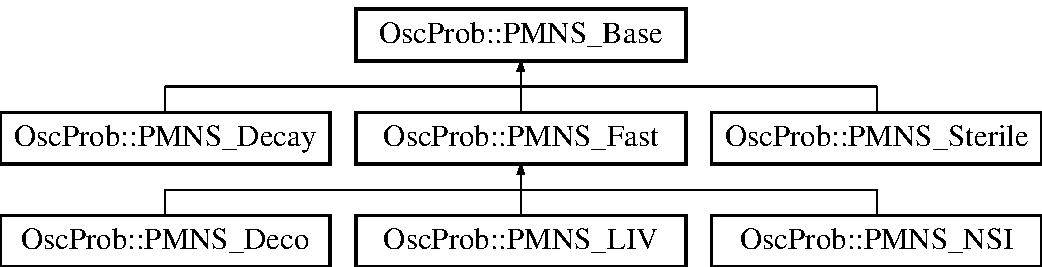
\includegraphics[height=3.000000cm]{classOscProb_1_1PMNS__Base}
\end{center}
\end{figure}
\subsection*{Public Member Functions}
\begin{DoxyCompactItemize}
\item 
\hyperlink{classOscProb_1_1PMNS__Base_aa53e83b03a9cf4bdfa0a07136bd17a79}{P\+M\+N\+S\+\_\+\+Base} (int num\+Nus=3)
\begin{DoxyCompactList}\small\item\em Constructor. \end{DoxyCompactList}\item 
virtual \hyperlink{classOscProb_1_1PMNS__Base_a91223a852214dd90da9b4403f779dbbf}{$\sim$\+P\+M\+N\+S\+\_\+\+Base} ()
\begin{DoxyCompactList}\small\item\em Destructor. \end{DoxyCompactList}\item 
virtual double \hyperlink{classOscProb_1_1PMNS__Base_aa2e10704d2d205a1ec8988de14b1a66f}{Prob} (std\+::vector$<$ \hyperlink{EigenPoint_8h_a67ca8e107e20610c3fff78d5e726ece0}{complexD} $>$ nu\+\_\+in, int flvf)
\begin{DoxyCompactList}\small\item\em Compute the probability of nu\+\_\+in going to flvf. \end{DoxyCompactList}\item 
virtual double \hyperlink{classOscProb_1_1PMNS__Base_a0190a79284289aacf682c78d7cef9a81}{Prob} (std\+::vector$<$ \hyperlink{EigenPoint_8h_a67ca8e107e20610c3fff78d5e726ece0}{complexD} $>$ nu\+\_\+in, int flvf, double E)
\begin{DoxyCompactList}\small\item\em Compute the probability of nu\+\_\+in going to flvf for energy E. \end{DoxyCompactList}\item 
virtual double \hyperlink{classOscProb_1_1PMNS__Base_a01fba31729345376705e02408e835f67}{Prob} (std\+::vector$<$ \hyperlink{EigenPoint_8h_a67ca8e107e20610c3fff78d5e726ece0}{complexD} $>$ nu\+\_\+in, int flvf, double E, double L)
\begin{DoxyCompactList}\small\item\em Compute the probability of nu\+\_\+in going to flvf for energy E and distance L. \end{DoxyCompactList}\item 
virtual double \hyperlink{classOscProb_1_1PMNS__Base_aec5c399b93261f1962a4b7dbbb44b973}{Prob} (int flvi, int flvf)
\begin{DoxyCompactList}\small\item\em Compute the probability of flvi going to flvf. \end{DoxyCompactList}\item 
virtual double \hyperlink{classOscProb_1_1PMNS__Base_aa3cee10639d5c0879ccb9e78d62128d3}{Prob} (int flvi, int flvf, double E)
\begin{DoxyCompactList}\small\item\em Compute the probability of flvi going to flvf for energy E. \end{DoxyCompactList}\item 
virtual double \hyperlink{classOscProb_1_1PMNS__Base_a6e0a74508d9d6db7be02e242b8467563}{Prob} (int flvi, int flvf, double E, double L)
\begin{DoxyCompactList}\small\item\em Compute the probability of flvi going to flvf for energy E and distance L. \end{DoxyCompactList}\item 
virtual double \hyperlink{classOscProb_1_1PMNS__Base_a89e54c80ae8a31effbab7b2b970606bb}{Avg\+Prob} (std\+::vector$<$ \hyperlink{EigenPoint_8h_a67ca8e107e20610c3fff78d5e726ece0}{complexD} $>$ nu\+\_\+in, int flvf, double E, double dE=0)
\begin{DoxyCompactList}\small\item\em Compute the average probability over a bin of energy. \end{DoxyCompactList}\item 
virtual double \hyperlink{classOscProb_1_1PMNS__Base_a19f160c045a01e5083506e925fb37d44}{Avg\+Prob\+LoE} (std\+::vector$<$ \hyperlink{EigenPoint_8h_a67ca8e107e20610c3fff78d5e726ece0}{complexD} $>$ nu\+\_\+in, int flvf, double LoE, double d\+LoE=0)
\begin{DoxyCompactList}\small\item\em Compute the average probability over a bin of L/E. \end{DoxyCompactList}\item 
virtual double \hyperlink{classOscProb_1_1PMNS__Base_ac03f754160422e6600da8dbae0f803ed}{Avg\+Prob} (int flvi, int flvf, double E, double dE=0)
\begin{DoxyCompactList}\small\item\em Compute the average probability over a bin of energy. \end{DoxyCompactList}\item 
virtual double \hyperlink{classOscProb_1_1PMNS__Base_ac19a92f4ef428a7333ca8eed76fca637}{Avg\+Prob\+LoE} (int flvi, int flvf, double LoE, double d\+LoE=0)
\begin{DoxyCompactList}\small\item\em Compute the average probability over a bin of L/E. \end{DoxyCompactList}\item 
virtual std\+::vector$<$ \hyperlink{EigenPoint_8h_a67ca8e107e20610c3fff78d5e726ece0}{complexD} $>$ \hyperlink{classOscProb_1_1PMNS__Base_a5092561dd8579d390c649eb60803ea98}{Get\+Mass\+Eigenstate} (int mi)
\begin{DoxyCompactList}\small\item\em Get a neutrino mass eigenstate. \end{DoxyCompactList}\item 
virtual void \hyperlink{classOscProb_1_1PMNS__Base_ace7875cf6d3bec161a2b7ed2690aec34}{Set\+Angle} (int i, int j, double th)
\begin{DoxyCompactList}\small\item\em Set the mixing angle theta\+\_\+ij. \end{DoxyCompactList}\item 
virtual void \hyperlink{classOscProb_1_1PMNS__Base_a4bef78cfcfc4e70b4ce79cdb8862c0a3}{Set\+Delta} (int i, int j, double delta)
\begin{DoxyCompactList}\small\item\em Set the CP phase delta\+\_\+ij. \end{DoxyCompactList}\item 
virtual void \hyperlink{classOscProb_1_1PMNS__Base_a492243b22fb1b783cd2943f507cff970}{Set\+Dm} (int j, double dm)
\begin{DoxyCompactList}\small\item\em Set the mass-\/splitting dm\+\_\+j1 in e\+V$^\wedge$2. \end{DoxyCompactList}\item 
virtual double \hyperlink{classOscProb_1_1PMNS__Base_acee137091304c919642293ddf015bbc8}{Get\+Angle} (int i, int j)
\begin{DoxyCompactList}\small\item\em Get the mixing angle theta\+\_\+ij. \end{DoxyCompactList}\item 
virtual double \hyperlink{classOscProb_1_1PMNS__Base_adb8dbc91d4286d2e7c8f768c59476241}{Get\+Delta} (int i, int j)
\begin{DoxyCompactList}\small\item\em Get the CP phase delta\+\_\+ij. \end{DoxyCompactList}\item 
virtual double \hyperlink{classOscProb_1_1PMNS__Base_ad26815ac5f4805d1259817e4936e5f8f}{Get\+Dm} (int j)
\begin{DoxyCompactList}\small\item\em Get the mass-\/splitting dm\+\_\+j1 in e\+V$^\wedge$2. \end{DoxyCompactList}\item 
virtual double \hyperlink{classOscProb_1_1PMNS__Base_a4ea861a6707ce1be3a54aad2b60f8632}{Get\+Dm\+Eff} (int j)
\begin{DoxyCompactList}\small\item\em Get the effective mass-\/splitting dm\+\_\+j1 in e\+V$^\wedge$2. \end{DoxyCompactList}\item 
virtual void \hyperlink{classOscProb_1_1PMNS__Base_a4de96ac9b6d1e9b029ab877e57d211ad}{Set\+Std\+Pars} ()
\begin{DoxyCompactList}\small\item\em Set P\+DG 3-\/flavor parameters. \end{DoxyCompactList}\item 
virtual void \hyperlink{classOscProb_1_1PMNS__Base_a95b3b0d0cab5e6a54b5ef99587f837c0}{Set\+Energy} (double E)
\begin{DoxyCompactList}\small\item\em Set the neutrino energy in GeV. \end{DoxyCompactList}\item 
virtual void \hyperlink{classOscProb_1_1PMNS__Base_a717e0348cf762f3961854e332a9b52e0}{Set\+Is\+Nu\+Bar} (bool is\+Nu\+Bar)
\begin{DoxyCompactList}\small\item\em Set the anti-\/neutrino flag. \end{DoxyCompactList}\item 
virtual double \hyperlink{classOscProb_1_1PMNS__Base_acc0d46cc4b8f911b40b807225003bbed}{Get\+Energy} ()
\begin{DoxyCompactList}\small\item\em Get the neutrino energy in GeV. \end{DoxyCompactList}\item 
virtual bool \hyperlink{classOscProb_1_1PMNS__Base_a2f7f2a028dfe7a90fff6b4f757972c2c}{Get\+Is\+Nu\+Bar} ()
\begin{DoxyCompactList}\small\item\em Get the anti-\/neutrino flag. \end{DoxyCompactList}\item 
virtual void \hyperlink{classOscProb_1_1PMNS__Base_ac3b644fd0a56347d304ceca4ae9d8875}{Set\+Path} (\hyperlink{structOscProb_1_1NuPath}{Osc\+Prob\+::\+Nu\+Path} p)
\begin{DoxyCompactList}\small\item\em Set a single path. \end{DoxyCompactList}\item 
virtual void \hyperlink{classOscProb_1_1PMNS__Base_a35b983270613072a3df58b574d80dbfd}{Set\+Path} (double length, double density, double zoa=0.\+5, int layer=0)
\begin{DoxyCompactList}\small\item\em Set a single path. \end{DoxyCompactList}\item 
virtual void \hyperlink{classOscProb_1_1PMNS__Base_a637d19dd850b4246507796526622643c}{Set\+Path} (std\+::vector$<$ \hyperlink{structOscProb_1_1NuPath}{Osc\+Prob\+::\+Nu\+Path} $>$ paths)
\begin{DoxyCompactList}\small\item\em Set a path sequence. \end{DoxyCompactList}\item 
virtual void \hyperlink{classOscProb_1_1PMNS__Base_a887dc9d4dc569ec0cdef3933b4c60efc}{Add\+Path} (\hyperlink{structOscProb_1_1NuPath}{Osc\+Prob\+::\+Nu\+Path} p)
\begin{DoxyCompactList}\small\item\em Add a path to the sequence. \end{DoxyCompactList}\item 
virtual void \hyperlink{classOscProb_1_1PMNS__Base_ab7f89ad9e7e1224adaa59d3c41594cd9}{Add\+Path} (double length, double density, double zoa=0.\+5, int layer=0)
\begin{DoxyCompactList}\small\item\em Add a path to the sequence. \end{DoxyCompactList}\item 
virtual void \hyperlink{classOscProb_1_1PMNS__Base_aefe521239031c418cfaaaa550a6e13bb}{Clear\+Path} ()
\begin{DoxyCompactList}\small\item\em Clear the path vector. \end{DoxyCompactList}\item 
virtual void \hyperlink{classOscProb_1_1PMNS__Base_a6241325b1bd28cafa556daaecbe4ed62}{Set\+Length} (double L)
\begin{DoxyCompactList}\small\item\em Set a single path lentgh in km. \end{DoxyCompactList}\item 
virtual void \hyperlink{classOscProb_1_1PMNS__Base_ac74206f349687da141392c81e2ba6b0d}{Set\+Density} (double rho)
\begin{DoxyCompactList}\small\item\em Set single path density in g/cm$^\wedge$3. \end{DoxyCompactList}\item 
virtual void \hyperlink{classOscProb_1_1PMNS__Base_a1bf3ea8fd2507fd2fd82d7410ff8f578}{Set\+ZoA} (double zoa)
\begin{DoxyCompactList}\small\item\em Set Z/A value for single path. \end{DoxyCompactList}\item 
virtual void \hyperlink{classOscProb_1_1PMNS__Base_aa34a40a3b5abda0f252982d9ead3b520}{Set\+Length} (std\+::vector$<$ double $>$ L)
\begin{DoxyCompactList}\small\item\em Set multiple path lengths. \end{DoxyCompactList}\item 
virtual void \hyperlink{classOscProb_1_1PMNS__Base_a858221d5510fe732dc6a101fd305cda0}{Set\+Density} (std\+::vector$<$ double $>$ rho)
\begin{DoxyCompactList}\small\item\em Set multiple path densities. \end{DoxyCompactList}\item 
virtual void \hyperlink{classOscProb_1_1PMNS__Base_a8495f8a320e1a21965e6a64aec92ad2a}{Set\+ZoA} (std\+::vector$<$ double $>$ zoa)
\begin{DoxyCompactList}\small\item\em Set multiple path Z/A values. \end{DoxyCompactList}\item 
virtual void \hyperlink{classOscProb_1_1PMNS__Base_a904e580edf89fb98bf9a6397739b4ebe}{Set\+Layers} (std\+::vector$<$ int $>$ lay)
\begin{DoxyCompactList}\small\item\em Set multiple path layer indices. \end{DoxyCompactList}\item 
virtual void \hyperlink{classOscProb_1_1PMNS__Base_add6533a9fc9acdfc7ae258b62570d78d}{Set\+Std\+Path} ()
\begin{DoxyCompactList}\small\item\em Set standard neutrino path. \end{DoxyCompactList}\item 
virtual std\+::vector$<$ \hyperlink{structOscProb_1_1NuPath}{Osc\+Prob\+::\+Nu\+Path} $>$ \hyperlink{classOscProb_1_1PMNS__Base_ac8e196f2e85a2b1caaf705073ee95a5c}{Get\+Path} ()
\begin{DoxyCompactList}\small\item\em Get the neutrino path sequence. \end{DoxyCompactList}\item 
virtual std\+::vector$<$ double $>$ \hyperlink{classOscProb_1_1PMNS__Base_a9eac8d768c1424755ee41f7e783af179}{Get\+Sample\+Points} (double LoE, double d\+LoE)
\begin{DoxyCompactList}\small\item\em Compute the sample points for a bin of L/E with width d\+LoE. \end{DoxyCompactList}\item 
virtual void \hyperlink{classOscProb_1_1PMNS__Base_aa94c1e1fff0ba731c75f7e633b023a9f}{Set\+Use\+Cache} (bool u=true)
\begin{DoxyCompactList}\small\item\em Set caching on/off. \end{DoxyCompactList}\item 
virtual void \hyperlink{classOscProb_1_1PMNS__Base_ac47fd33e69aa6490f99e2fd147a92f03}{Clear\+Cache} ()
\begin{DoxyCompactList}\small\item\em Clear the cache. \end{DoxyCompactList}\item 
virtual void \hyperlink{classOscProb_1_1PMNS__Base_ae67862cf58b0802487a14b047b012a78}{Set\+Max\+Cache} (int mc=1e6)
\begin{DoxyCompactList}\small\item\em Set max cache size. \end{DoxyCompactList}\end{DoxyCompactItemize}
\subsection*{Protected Member Functions}
\begin{DoxyCompactItemize}
\item 
virtual void \hyperlink{classOscProb_1_1PMNS__Base_adf23b569112f9f9e0e592f01d79a5f3d}{Initialize\+Vectors} ()
\begin{DoxyCompactList}\small\item\em Initialize all member vectors with zeros. \end{DoxyCompactList}\item 
virtual bool \hyperlink{classOscProb_1_1PMNS__Base_abe533da5f64bec1f4724ab7b58606b77}{Try\+Cache} ()
\begin{DoxyCompactList}\small\item\em Try to find a cached eigensystem. \end{DoxyCompactList}\item 
virtual void \hyperlink{classOscProb_1_1PMNS__Base_a785c37fcea974628623c8881bb0fbbf9}{Fill\+Cache} ()
\begin{DoxyCompactList}\small\item\em Cache the current eigensystem. \end{DoxyCompactList}\item 
virtual void \hyperlink{classOscProb_1_1PMNS__Base_a986e6ebef09a7e2eb7fee16a4c2c834d}{Set\+Cur\+Path} (\hyperlink{structOscProb_1_1NuPath}{Osc\+Prob\+::\+Nu\+Path} p)
\begin{DoxyCompactList}\small\item\em Set the path currently in use by the class. \end{DoxyCompactList}\item 
virtual void \hyperlink{classOscProb_1_1PMNS__Base_aba565962a440d14bee7a2a96d2eca2c5}{Set\+Att} (double att, int idx)
\begin{DoxyCompactList}\small\item\em Set one of the path attributes. \end{DoxyCompactList}\item 
virtual void \hyperlink{classOscProb_1_1PMNS__Base_aa001479b5f5828c3d16ed087f96ecbcc}{Set\+Att} (std\+::vector$<$ double $>$ att, int idx)
\begin{DoxyCompactList}\small\item\em Set all values of a path attribute. \end{DoxyCompactList}\item 
virtual void \hyperlink{classOscProb_1_1PMNS__Base_a6a3cf45bbe2349abf06708b65677c044}{RotateH} (int i, int j, std\+::vector$<$ std\+::vector$<$ \hyperlink{EigenPoint_8h_a67ca8e107e20610c3fff78d5e726ece0}{complexD} $>$ $>$ \&Ham)
\begin{DoxyCompactList}\small\item\em Rotate the Hamiltonian by theta\+\_\+ij and delta\+\_\+ij. \end{DoxyCompactList}\item 
virtual void \hyperlink{classOscProb_1_1PMNS__Base_ae52554477ad3250daa5adb8c32cab0b4}{Rotate\+State} (int i, int j)
\begin{DoxyCompactList}\small\item\em Rotate the neutrino state by theta\+\_\+ij and delta\+\_\+ij. \end{DoxyCompactList}\item 
virtual void \hyperlink{classOscProb_1_1PMNS__Base_ad0faf5eae755afb1baa1fcd5ffebad41}{Build\+Hms} ()
\begin{DoxyCompactList}\small\item\em Build the matrix of masses squared. \end{DoxyCompactList}\item 
virtual void \hyperlink{classOscProb_1_1PMNS__Base_a91f065cb9e910e0095e41462b4420b01}{Solve\+Ham} ()=0
\begin{DoxyCompactList}\small\item\em Solve the full Hamiltonian for eigenvectors and eigenvalues. \end{DoxyCompactList}\item 
virtual void \hyperlink{classOscProb_1_1PMNS__Base_ac0d4bf8ff1318ef96d3dafa62e0cec25}{Reset\+To\+Flavour} (int flv)
\begin{DoxyCompactList}\small\item\em Reset neutrino state to pure flavour flv. \end{DoxyCompactList}\item 
virtual void \hyperlink{classOscProb_1_1PMNS__Base_accb08503acc162188041d7a96a280462}{Propagate\+Path} (\hyperlink{structOscProb_1_1NuPath}{Osc\+Prob\+::\+Nu\+Path} p)
\begin{DoxyCompactList}\small\item\em Propagate neutrino through a single path. \end{DoxyCompactList}\item 
virtual void \hyperlink{classOscProb_1_1PMNS__Base_a054e3a8b05b9a958b6fa416e4a835e3e}{Propagate} ()
\begin{DoxyCompactList}\small\item\em Propagate neutrino through full path. \end{DoxyCompactList}\item 
virtual double \hyperlink{classOscProb_1_1PMNS__Base_a0dc4d45bc3d7e03b9abbf5b4e100cc22}{P} (int flv)
\begin{DoxyCompactList}\small\item\em Return the probability of final state in flavour flv. \end{DoxyCompactList}\end{DoxyCompactItemize}
\subsection*{Protected Attributes}
\begin{DoxyCompactItemize}
\item 
int \hyperlink{classOscProb_1_1PMNS__Base_a24bb74bed63569dfe88b18fa6a08060e}{f\+Num\+Nus}
\begin{DoxyCompactList}\small\item\em Number of neutrino flavours. \end{DoxyCompactList}\item 
std\+::vector$<$ double $>$ \hyperlink{classOscProb_1_1PMNS__Base_a406a31c3b5d620e5a0cace5b411f9f70}{f\+Dm}
\begin{DoxyCompactList}\small\item\em m$^\wedge$2\+\_\+i -\/ m$^\wedge$2\+\_\+1 in vacuum \end{DoxyCompactList}\item 
std\+::vector$<$ std\+::vector$<$ double $>$ $>$ \hyperlink{classOscProb_1_1PMNS__Base_a1976887cd658dd86b2336c181f1470b4}{f\+Theta}
\begin{DoxyCompactList}\small\item\em theta\mbox{[}i\mbox{]}\mbox{[}j\mbox{]} mixing angle \end{DoxyCompactList}\item 
std\+::vector$<$ std\+::vector$<$ double $>$ $>$ \hyperlink{classOscProb_1_1PMNS__Base_ab2a5fa40e689b221c8a7d2c17213810d}{f\+Delta}
\begin{DoxyCompactList}\small\item\em delta\mbox{[}i\mbox{]}\mbox{[}j\mbox{]} CP violating phase \end{DoxyCompactList}\item 
std\+::vector$<$ \hyperlink{EigenPoint_8h_a67ca8e107e20610c3fff78d5e726ece0}{complexD} $>$ \hyperlink{classOscProb_1_1PMNS__Base_abf99f2339e3ee989600740b5d88063e8}{f\+Nu\+State}
\begin{DoxyCompactList}\small\item\em The neutrino current state. \end{DoxyCompactList}\item 
std\+::vector$<$ std\+::vector$<$ \hyperlink{EigenPoint_8h_a67ca8e107e20610c3fff78d5e726ece0}{complexD} $>$ $>$ \hyperlink{classOscProb_1_1PMNS__Base_acd3c8783e7603081eab316ea4c86c766}{f\+Hms}
\begin{DoxyCompactList}\small\item\em matrix H$\ast$2E in e\+V$^\wedge$2 \end{DoxyCompactList}\item 
std\+::vector$<$ \hyperlink{EigenPoint_8h_a67ca8e107e20610c3fff78d5e726ece0}{complexD} $>$ \hyperlink{classOscProb_1_1PMNS__Base_ab8d26b722047d49d977f5f2d83026ede}{f\+Phases}
\begin{DoxyCompactList}\small\item\em Buffer for oscillation phases. \end{DoxyCompactList}\item 
std\+::vector$<$ \hyperlink{EigenPoint_8h_a67ca8e107e20610c3fff78d5e726ece0}{complexD} $>$ \hyperlink{classOscProb_1_1PMNS__Base_a5440bc3efa466a37649601abce559e3e}{f\+Buffer}
\begin{DoxyCompactList}\small\item\em Buffer for neutrino state tranformations. \end{DoxyCompactList}\item 
std\+::vector$<$ double $>$ \hyperlink{classOscProb_1_1PMNS__Base_a6319c34d7decbb9d7d6da279c06e8c2d}{f\+Eval}
\begin{DoxyCompactList}\small\item\em Eigenvalues of the Hamiltonian. \end{DoxyCompactList}\item 
std\+::vector$<$ std\+::vector$<$ \hyperlink{EigenPoint_8h_a67ca8e107e20610c3fff78d5e726ece0}{complexD} $>$ $>$ \hyperlink{classOscProb_1_1PMNS__Base_a87be137356c5f27ab83cab5e1298ef8f}{f\+Evec}
\begin{DoxyCompactList}\small\item\em Eigenvectors of the Hamiltonian. \end{DoxyCompactList}\item 
double \hyperlink{classOscProb_1_1PMNS__Base_a2800af6d436972f3e900867790c046b0}{f\+Energy}
\begin{DoxyCompactList}\small\item\em Neutrino energy. \end{DoxyCompactList}\item 
bool \hyperlink{classOscProb_1_1PMNS__Base_a0ebaeaefab36a3ff381c6293faedfdd6}{f\+Is\+Nu\+Bar}
\begin{DoxyCompactList}\small\item\em Anti-\/neutrino flag. \end{DoxyCompactList}\item 
std\+::vector$<$ \hyperlink{structOscProb_1_1NuPath}{Osc\+Prob\+::\+Nu\+Path} $>$ \hyperlink{classOscProb_1_1PMNS__Base_a69db9d57e12fc7cbe0431bc6c18fac93}{f\+Nu\+Paths}
\begin{DoxyCompactList}\small\item\em Vector of neutrino paths. \end{DoxyCompactList}\item 
\hyperlink{structOscProb_1_1NuPath}{Osc\+Prob\+::\+Nu\+Path} \hyperlink{classOscProb_1_1PMNS__Base_a849437aa8891fe042e86886ce8f81c6e}{f\+Path}
\begin{DoxyCompactList}\small\item\em Current neutrino path. \end{DoxyCompactList}\item 
bool \hyperlink{classOscProb_1_1PMNS__Base_a9ac3cadeac8db1b90f3152f476244780}{f\+Built\+Hms}
\begin{DoxyCompactList}\small\item\em Tag to avoid rebuilding Hms. \end{DoxyCompactList}\item 
bool \hyperlink{classOscProb_1_1PMNS__Base_a6dc5cd010d2d70b2324745b4e53e9839}{f\+Got\+ES}
\begin{DoxyCompactList}\small\item\em Tag to avoid recalculating eigensystem. \end{DoxyCompactList}\item 
bool \hyperlink{classOscProb_1_1PMNS__Base_ad28c12ef897b5555eda509ea55c99107}{f\+Use\+Cache}
\begin{DoxyCompactList}\small\item\em Flag for whether to use caching. \end{DoxyCompactList}\item 
double \hyperlink{classOscProb_1_1PMNS__Base_a0b4c41a27de281472453a1912cbc1e64}{f\+Cache\+Prec}
\begin{DoxyCompactList}\small\item\em Precision of cache matching. \end{DoxyCompactList}\item 
int \hyperlink{classOscProb_1_1PMNS__Base_a74c13356eafec2490d8c3c19759ba7f0}{f\+Max\+Cache}
\begin{DoxyCompactList}\small\item\em Maximum cache size. \end{DoxyCompactList}\item 
std\+::set$<$ \hyperlink{structOscProb_1_1EigenPoint}{Osc\+Prob\+::\+Eigen\+Point} $>$ \hyperlink{classOscProb_1_1PMNS__Base_a8159424f20197a3a7145fe3bf2c11176}{f\+Mix\+Cache}
\begin{DoxyCompactList}\small\item\em Caching set of eigensystems. \end{DoxyCompactList}\item 
\hyperlink{structOscProb_1_1EigenPoint}{Eigen\+Point} \hyperlink{classOscProb_1_1PMNS__Base_ab1fe4800ee3ae48df4fc942dce00e0d3}{f\+Probe}
\begin{DoxyCompactList}\small\item\em Eigenp\+Point to try. \end{DoxyCompactList}\end{DoxyCompactItemize}
\subsection*{Static Protected Attributes}
\begin{DoxyCompactItemize}
\item 
static const \hyperlink{EigenPoint_8h_a67ca8e107e20610c3fff78d5e726ece0}{complexD} \hyperlink{classOscProb_1_1PMNS__Base_a05e595848c2521dc795efa7645728b94}{zero}
\begin{DoxyCompactList}\small\item\em zero in complex \end{DoxyCompactList}\item 
static const \hyperlink{EigenPoint_8h_a67ca8e107e20610c3fff78d5e726ece0}{complexD} \hyperlink{classOscProb_1_1PMNS__Base_a7d1d0bbcab30a1fd8c368c40134c51ff}{one}
\begin{DoxyCompactList}\small\item\em one in complex \end{DoxyCompactList}\item 
static const double \hyperlink{classOscProb_1_1PMNS__Base_a382ddd7b76ca89b43f22614a2ea7327b}{k\+Km2eV} = 1.\+0 / 1.\+973269788e-\/10
\begin{DoxyCompactList}\small\item\em km to e\+V$^\wedge$-\/1 \end{DoxyCompactList}\item 
static const double \hyperlink{classOscProb_1_1PMNS__Base_a326fc5016d7dd7ce05682c06cdcb6d94}{k\+K2} = 1e-\/3 $\ast$ k\+N\+A / pow(k\+Km2e\+V,3)
\begin{DoxyCompactList}\small\item\em mol/\+Ge\+V$^\wedge$2/cm$^\wedge$3 to eV \end{DoxyCompactList}\item 
static const double \hyperlink{classOscProb_1_1PMNS__Base_ad36a0a6bf58d6ec093d3947784bd89e9}{k\+Ge\+V2eV} = 1.\+0e+09
\begin{DoxyCompactList}\small\item\em GeV to eV. \end{DoxyCompactList}\item 
static const double \hyperlink{classOscProb_1_1PMNS__Base_a69355e770b89e99437c2b8a66e48eeb9}{k\+NA} = 6.\+022140857e23
\begin{DoxyCompactList}\small\item\em Avogadro constant. \end{DoxyCompactList}\item 
static const double \hyperlink{classOscProb_1_1PMNS__Base_a7f26a3456128234b2ae6cc9141a6532f}{k\+Gf} = 1.\+1663787e-\/05
\begin{DoxyCompactList}\small\item\em G\+\_\+F in units of Ge\+V$^\wedge$-\/2. \end{DoxyCompactList}\end{DoxyCompactItemize}


\subsection{Detailed Description}
This is an abstract class implementing the general functions needed for setting up an oscillation calculator. The method for solving the eigensystem for the Hamiltonian must be defined in the derived classes.

\begin{DoxySeeAlso}{See also}
\hyperlink{classOscProb_1_1PMNS__Fast}{P\+M\+N\+S\+\_\+\+Fast} \hyperlink{classOscProb_1_1PMNS__NSI}{P\+M\+N\+S\+\_\+\+N\+SI} \hyperlink{classOscProb_1_1PMNS__Sterile}{P\+M\+N\+S\+\_\+\+Sterile}
\end{DoxySeeAlso}
\begin{DoxyAuthor}{Author}
Joao Coelho -\/ coelho@lal.\+in2p3.\+fr 
\end{DoxyAuthor}


Definition at line 27 of file P\+M\+N\+S\+\_\+\+Base.\+h.



\subsection{Constructor \& Destructor Documentation}
\mbox{\Hypertarget{classOscProb_1_1PMNS__Base_aa53e83b03a9cf4bdfa0a07136bd17a79}\label{classOscProb_1_1PMNS__Base_aa53e83b03a9cf4bdfa0a07136bd17a79}} 
\index{Osc\+Prob\+::\+P\+M\+N\+S\+\_\+\+Base@{Osc\+Prob\+::\+P\+M\+N\+S\+\_\+\+Base}!P\+M\+N\+S\+\_\+\+Base@{P\+M\+N\+S\+\_\+\+Base}}
\index{P\+M\+N\+S\+\_\+\+Base@{P\+M\+N\+S\+\_\+\+Base}!Osc\+Prob\+::\+P\+M\+N\+S\+\_\+\+Base@{Osc\+Prob\+::\+P\+M\+N\+S\+\_\+\+Base}}
\subsubsection{\texorpdfstring{P\+M\+N\+S\+\_\+\+Base()}{PMNS\_Base()}}
{\footnotesize\ttfamily P\+M\+N\+S\+\_\+\+Base\+::\+P\+M\+N\+S\+\_\+\+Base (\begin{DoxyParamCaption}\item[{int}]{num\+Nus = {\ttfamily 3} }\end{DoxyParamCaption})}

Constructor.

Sets the number of neutrinos and initializes attributes

Default starts with a 2 GeV muon neutrino.

Path is set to the default 1000 km in crust density.

Oscillation parameters are from P\+DG for NH by default.


\begin{DoxyParams}{Parameters}
{\em num\+Nus} & -\/ the number of neutrino flavours \\
\hline
\end{DoxyParams}


Definition at line 48 of file P\+M\+N\+S\+\_\+\+Base.\+cxx.



References f\+Num\+Nus, Initialize\+Vectors(), Reset\+To\+Flavour(), Set\+Energy(), Set\+Is\+Nu\+Bar(), Set\+Std\+Pars(), Set\+Std\+Path(), and Set\+Use\+Cache().


\begin{DoxyCode}
48                                :
49 \hyperlink{classOscProb_1_1PMNS__Base_a6dc5cd010d2d70b2324745b4e53e9839}{fGotES}(\textcolor{keyword}{false}), \hyperlink{classOscProb_1_1PMNS__Base_a9ac3cadeac8db1b90f3152f476244780}{fBuiltHms}(\textcolor{keyword}{false}), \hyperlink{classOscProb_1_1PMNS__Base_a74c13356eafec2490d8c3c19759ba7f0}{fMaxCache}(1e6), \hyperlink{classOscProb_1_1PMNS__Base_ab1fe4800ee3ae48df4fc942dce00e0d3}{fProbe}(numNus)
50 \{
51 
52   \hyperlink{classOscProb_1_1PMNS__Base_aa94c1e1fff0ba731c75f7e633b023a9f}{SetUseCache}(\textcolor{keyword}{false});  \textcolor{comment}{// Don't cache eigensystems}
53 
54   \hyperlink{classOscProb_1_1PMNS__Base_a24bb74bed63569dfe88b18fa6a08060e}{fNumNus} = numNus;    \textcolor{comment}{// Set the number of neutrinos}
55 
56   \hyperlink{classOscProb_1_1PMNS__Base_add6533a9fc9acdfc7ae258b62570d78d}{SetStdPath}();        \textcolor{comment}{// Set some default path}
57   \hyperlink{classOscProb_1_1PMNS__Base_a95b3b0d0cab5e6a54b5ef99587f837c0}{SetEnergy}(2);        \textcolor{comment}{// Set default energy to 2 GeV}
58   \hyperlink{classOscProb_1_1PMNS__Base_a717e0348cf762f3961854e332a9b52e0}{SetIsNuBar}(\textcolor{keyword}{false});   \textcolor{comment}{// Neutrino by default}
59 
60   \hyperlink{classOscProb_1_1PMNS__Base_adf23b569112f9f9e0e592f01d79a5f3d}{InitializeVectors}(); \textcolor{comment}{// Initialize all vectors}
61 
62   \hyperlink{classOscProb_1_1PMNS__Base_a4de96ac9b6d1e9b029ab877e57d211ad}{SetStdPars}();        \textcolor{comment}{// Set PDG parameters}
63 
64   \hyperlink{classOscProb_1_1PMNS__Base_ac0d4bf8ff1318ef96d3dafa62e0cec25}{ResetToFlavour}(1);   \textcolor{comment}{// Numu by default}
65   
66 \}
\end{DoxyCode}
\mbox{\Hypertarget{classOscProb_1_1PMNS__Base_a91223a852214dd90da9b4403f779dbbf}\label{classOscProb_1_1PMNS__Base_a91223a852214dd90da9b4403f779dbbf}} 
\index{Osc\+Prob\+::\+P\+M\+N\+S\+\_\+\+Base@{Osc\+Prob\+::\+P\+M\+N\+S\+\_\+\+Base}!````~P\+M\+N\+S\+\_\+\+Base@{$\sim$\+P\+M\+N\+S\+\_\+\+Base}}
\index{````~P\+M\+N\+S\+\_\+\+Base@{$\sim$\+P\+M\+N\+S\+\_\+\+Base}!Osc\+Prob\+::\+P\+M\+N\+S\+\_\+\+Base@{Osc\+Prob\+::\+P\+M\+N\+S\+\_\+\+Base}}
\subsubsection{\texorpdfstring{$\sim$\+P\+M\+N\+S\+\_\+\+Base()}{~PMNS\_Base()}}
{\footnotesize\ttfamily P\+M\+N\+S\+\_\+\+Base\+::$\sim$\+P\+M\+N\+S\+\_\+\+Base (\begin{DoxyParamCaption}{ }\end{DoxyParamCaption})\hspace{0.3cm}{\ttfamily [virtual]}}

Nothing to clean. 

Definition at line 72 of file P\+M\+N\+S\+\_\+\+Base.\+cxx.


\begin{DoxyCode}
72 \{\}
\end{DoxyCode}


\subsection{Member Function Documentation}
\mbox{\Hypertarget{classOscProb_1_1PMNS__Base_a887dc9d4dc569ec0cdef3933b4c60efc}\label{classOscProb_1_1PMNS__Base_a887dc9d4dc569ec0cdef3933b4c60efc}} 
\index{Osc\+Prob\+::\+P\+M\+N\+S\+\_\+\+Base@{Osc\+Prob\+::\+P\+M\+N\+S\+\_\+\+Base}!Add\+Path@{Add\+Path}}
\index{Add\+Path@{Add\+Path}!Osc\+Prob\+::\+P\+M\+N\+S\+\_\+\+Base@{Osc\+Prob\+::\+P\+M\+N\+S\+\_\+\+Base}}
\subsubsection{\texorpdfstring{Add\+Path()}{AddPath()}\hspace{0.1cm}{\footnotesize\ttfamily [1/2]}}
{\footnotesize\ttfamily void P\+M\+N\+S\+\_\+\+Base\+::\+Add\+Path (\begin{DoxyParamCaption}\item[{\hyperlink{structOscProb_1_1NuPath}{Osc\+Prob\+::\+Nu\+Path}}]{p }\end{DoxyParamCaption})\hspace{0.3cm}{\ttfamily [virtual]}}

Add a path to the sequence. 
\begin{DoxyParams}{Parameters}
{\em p} & -\/ A neutrino path segment \\
\hline
\end{DoxyParams}


Definition at line 351 of file P\+M\+N\+S\+\_\+\+Base.\+cxx.



References f\+Nu\+Paths.



Referenced by Add\+Path(), Set\+Att(), and Set\+Path().


\begin{DoxyCode}
351                                \{
352 
353   \hyperlink{classOscProb_1_1PMNS__Base_a69db9d57e12fc7cbe0431bc6c18fac93}{fNuPaths}.push\_back(p);
354 
355 \}
\end{DoxyCode}
\mbox{\Hypertarget{classOscProb_1_1PMNS__Base_ab7f89ad9e7e1224adaa59d3c41594cd9}\label{classOscProb_1_1PMNS__Base_ab7f89ad9e7e1224adaa59d3c41594cd9}} 
\index{Osc\+Prob\+::\+P\+M\+N\+S\+\_\+\+Base@{Osc\+Prob\+::\+P\+M\+N\+S\+\_\+\+Base}!Add\+Path@{Add\+Path}}
\index{Add\+Path@{Add\+Path}!Osc\+Prob\+::\+P\+M\+N\+S\+\_\+\+Base@{Osc\+Prob\+::\+P\+M\+N\+S\+\_\+\+Base}}
\subsubsection{\texorpdfstring{Add\+Path()}{AddPath()}\hspace{0.1cm}{\footnotesize\ttfamily [2/2]}}
{\footnotesize\ttfamily void P\+M\+N\+S\+\_\+\+Base\+::\+Add\+Path (\begin{DoxyParamCaption}\item[{double}]{length,  }\item[{double}]{density,  }\item[{double}]{zoa = {\ttfamily 0.5},  }\item[{int}]{layer = {\ttfamily 0} }\end{DoxyParamCaption})\hspace{0.3cm}{\ttfamily [virtual]}}

Add a path to the sequence defining attributes directly. 
\begin{DoxyParams}{Parameters}
{\em length} & -\/ The length of the path segment in km \\
\hline
{\em density} & -\/ The density of the path segment in g/cm$^\wedge$3 \\
\hline
{\em zoa} & -\/ The effective Z/A of the path segment \\
\hline
{\em layer} & -\/ An index to identify the layer type (e.\+g. earth inner core) \\
\hline
\end{DoxyParams}


Definition at line 365 of file P\+M\+N\+S\+\_\+\+Base.\+cxx.



References Add\+Path().


\begin{DoxyCode}
365                                                                            \{
366 
367   \hyperlink{classOscProb_1_1PMNS__Base_a887dc9d4dc569ec0cdef3933b4c60efc}{AddPath}(\hyperlink{structOscProb_1_1NuPath}{NuPath}(length, density, zoa, layer));
368 
369 \}
\end{DoxyCode}
\mbox{\Hypertarget{classOscProb_1_1PMNS__Base_a89e54c80ae8a31effbab7b2b970606bb}\label{classOscProb_1_1PMNS__Base_a89e54c80ae8a31effbab7b2b970606bb}} 
\index{Osc\+Prob\+::\+P\+M\+N\+S\+\_\+\+Base@{Osc\+Prob\+::\+P\+M\+N\+S\+\_\+\+Base}!Avg\+Prob@{Avg\+Prob}}
\index{Avg\+Prob@{Avg\+Prob}!Osc\+Prob\+::\+P\+M\+N\+S\+\_\+\+Base@{Osc\+Prob\+::\+P\+M\+N\+S\+\_\+\+Base}}
\subsubsection{\texorpdfstring{Avg\+Prob()}{AvgProb()}\hspace{0.1cm}{\footnotesize\ttfamily [1/2]}}
{\footnotesize\ttfamily double P\+M\+N\+S\+\_\+\+Base\+::\+Avg\+Prob (\begin{DoxyParamCaption}\item[{std\+::vector$<$ \hyperlink{EigenPoint_8h_a67ca8e107e20610c3fff78d5e726ece0}{complexD} $>$}]{nu\+\_\+in,  }\item[{int}]{flvf,  }\item[{double}]{E,  }\item[{double}]{dE = {\ttfamily 0} }\end{DoxyParamCaption})\hspace{0.3cm}{\ttfamily [virtual]}}

Compute the average probability of nu\+\_\+in going to flvf over a bin of energy E with width dE.

This gets transformed into L/E, since the oscillation terms have arguments linear in L/E and not E.

This function works best for single paths. In multiple paths the accuracy may be somewhat worse. If needed, average over smaller energy ranges.

Flavours are\+: 
\begin{DoxyPre}
  0 = nue, 1 = numu, 2 = nutau
  3 = sterile\_1, 4 = sterile\_2, etc.
\end{DoxyPre}
 
\begin{DoxyParams}{Parameters}
{\em nu\+\_\+in} & -\/ The neutrino initial state in flavour. \\
\hline
{\em flvf} & -\/ The neutrino final flavour. \\
\hline
{\em E} & -\/ The neutrino energy in the bin center in GeV \\
\hline
{\em dE} & -\/ The energy bin width in GeV\\
\hline
\end{DoxyParams}
\begin{DoxyReturn}{Returns}
Average neutrino oscillation probability 
\end{DoxyReturn}


Definition at line 1386 of file P\+M\+N\+S\+\_\+\+Base.\+cxx.



References Osc\+Prob\+::\+Avg\+Path(), Avg\+Prob\+Lo\+E(), f\+Nu\+Paths, f\+Path, Osc\+Prob\+::\+Nu\+Path\+::length, Prob(), and Set\+Cur\+Path().



Referenced by Avg\+Prob().


\begin{DoxyCode}
1387 \{
1388 
1389   \textcolor{comment}{// Do nothing if energy is not positive}
1390   \textcolor{keywordflow}{if}(E<=0) \textcolor{keywordflow}{return} 0;
1391 
1392   \textcolor{keywordflow}{if}(\hyperlink{classOscProb_1_1PMNS__Base_a69db9d57e12fc7cbe0431bc6c18fac93}{fNuPaths}.empty()) \textcolor{keywordflow}{return} 0;
1393 
1394   \textcolor{comment}{// Don't average zero width}
1395   \textcolor{keywordflow}{if}(dE<=0) \textcolor{keywordflow}{return} \hyperlink{classOscProb_1_1PMNS__Base_aa2e10704d2d205a1ec8988de14b1a66f}{Prob}(nu\_in, flvf, E);
1396 
1397   \textcolor{comment}{// Make sure fPath is set}
1398   \textcolor{comment}{// Use average if multiple paths}
1399   \hyperlink{classOscProb_1_1PMNS__Base_a986e6ebef09a7e2eb7fee16a4c2c834d}{SetCurPath}(\hyperlink{namespaceOscProb_a999a7944bad8bc72d7ee9f56f81a210e}{AvgPath}(\hyperlink{classOscProb_1_1PMNS__Base_a69db9d57e12fc7cbe0431bc6c18fac93}{fNuPaths}));
1400 
1401   \textcolor{comment}{// Define L/E variables}
1402   \textcolor{keywordtype}{double} LoE = 0;
1403   \textcolor{keywordtype}{double} dLoE = 0;
1404 
1405   \textcolor{comment}{// Set a minimum energy}
1406   \textcolor{keywordtype}{double} minE = 0.1 * E;
1407 
1408   \textcolor{comment}{// Transform range to L/E}
1409   \textcolor{comment}{// Full range if low edge > minE}
1410   \textcolor{keywordflow}{if}(E-dE/2 > minE)\{
1411     LoE = 0.5 * (\hyperlink{classOscProb_1_1PMNS__Base_a849437aa8891fe042e86886ce8f81c6e}{fPath}.\hyperlink{structOscProb_1_1NuPath_af22660894b6e25cf835500381b155557}{length}/(E-dE/2) + \hyperlink{classOscProb_1_1PMNS__Base_a849437aa8891fe042e86886ce8f81c6e}{fPath}.\hyperlink{structOscProb_1_1NuPath_af22660894b6e25cf835500381b155557}{length}/(E+dE/2));
1412     dLoE = \hyperlink{classOscProb_1_1PMNS__Base_a849437aa8891fe042e86886ce8f81c6e}{fPath}.\hyperlink{structOscProb_1_1NuPath_af22660894b6e25cf835500381b155557}{length}/(E-dE/2) - \hyperlink{classOscProb_1_1PMNS__Base_a849437aa8891fe042e86886ce8f81c6e}{fPath}.\hyperlink{structOscProb_1_1NuPath_af22660894b6e25cf835500381b155557}{length}/(E+dE/2);
1413   \}
1414   \textcolor{comment}{// Else start at minE}
1415   \textcolor{keywordflow}{else}\{
1416     LoE = 0.5 * (\hyperlink{classOscProb_1_1PMNS__Base_a849437aa8891fe042e86886ce8f81c6e}{fPath}.\hyperlink{structOscProb_1_1NuPath_af22660894b6e25cf835500381b155557}{length}/minE + \hyperlink{classOscProb_1_1PMNS__Base_a849437aa8891fe042e86886ce8f81c6e}{fPath}.\hyperlink{structOscProb_1_1NuPath_af22660894b6e25cf835500381b155557}{length}/(E+dE/2));
1417     dLoE = \hyperlink{classOscProb_1_1PMNS__Base_a849437aa8891fe042e86886ce8f81c6e}{fPath}.\hyperlink{structOscProb_1_1NuPath_af22660894b6e25cf835500381b155557}{length}/minE - \hyperlink{classOscProb_1_1PMNS__Base_a849437aa8891fe042e86886ce8f81c6e}{fPath}.\hyperlink{structOscProb_1_1NuPath_af22660894b6e25cf835500381b155557}{length}/(E+dE/2);
1418   \}
1419 
1420   \textcolor{comment}{// Compute average in LoE}
1421   \textcolor{keywordflow}{return} \hyperlink{classOscProb_1_1PMNS__Base_a19f160c045a01e5083506e925fb37d44}{AvgProbLoE}(nu\_in, flvf, LoE, dLoE);
1422 
1423 \}
\end{DoxyCode}
\mbox{\Hypertarget{classOscProb_1_1PMNS__Base_ac03f754160422e6600da8dbae0f803ed}\label{classOscProb_1_1PMNS__Base_ac03f754160422e6600da8dbae0f803ed}} 
\index{Osc\+Prob\+::\+P\+M\+N\+S\+\_\+\+Base@{Osc\+Prob\+::\+P\+M\+N\+S\+\_\+\+Base}!Avg\+Prob@{Avg\+Prob}}
\index{Avg\+Prob@{Avg\+Prob}!Osc\+Prob\+::\+P\+M\+N\+S\+\_\+\+Base@{Osc\+Prob\+::\+P\+M\+N\+S\+\_\+\+Base}}
\subsubsection{\texorpdfstring{Avg\+Prob()}{AvgProb()}\hspace{0.1cm}{\footnotesize\ttfamily [2/2]}}
{\footnotesize\ttfamily double P\+M\+N\+S\+\_\+\+Base\+::\+Avg\+Prob (\begin{DoxyParamCaption}\item[{int}]{flvi,  }\item[{int}]{flvf,  }\item[{double}]{E,  }\item[{double}]{dE = {\ttfamily 0} }\end{DoxyParamCaption})\hspace{0.3cm}{\ttfamily [virtual]}}

Compute the average probability of flvi going to flvf over a bin of energy E with width dE.

This gets transformed into L/E, since the oscillation terms have arguments linear in L/E and not E.

This function works best for single paths. In multiple paths the accuracy may be somewhat worse. If needed, average over smaller energy ranges.

Flavours are\+: 
\begin{DoxyPre}
  0 = nue, 1 = numu, 2 = nutau
  3 = sterile\_1, 4 = sterile\_2, etc.
\end{DoxyPre}
 
\begin{DoxyParams}{Parameters}
{\em flvi} & -\/ The neutrino starting flavour. \\
\hline
{\em flvf} & -\/ The neutrino final flavour. \\
\hline
{\em E} & -\/ The neutrino energy in the bin center in GeV \\
\hline
{\em dE} & -\/ The energy bin width in GeV\\
\hline
\end{DoxyParams}
\begin{DoxyReturn}{Returns}
Average neutrino oscillation probability 
\end{DoxyReturn}


Definition at line 1353 of file P\+M\+N\+S\+\_\+\+Base.\+cxx.



References Avg\+Prob(), f\+Nu\+State, and Reset\+To\+Flavour().


\begin{DoxyCode}
1354 \{
1355 
1356   \hyperlink{classOscProb_1_1PMNS__Base_ac0d4bf8ff1318ef96d3dafa62e0cec25}{ResetToFlavour}(flvi);
1357 
1358   \textcolor{keywordflow}{return} \hyperlink{classOscProb_1_1PMNS__Base_a89e54c80ae8a31effbab7b2b970606bb}{AvgProb}(\hyperlink{classOscProb_1_1PMNS__Base_abf99f2339e3ee989600740b5d88063e8}{fNuState}, flvf, E, dE);
1359 
1360 \}
\end{DoxyCode}
\mbox{\Hypertarget{classOscProb_1_1PMNS__Base_a19f160c045a01e5083506e925fb37d44}\label{classOscProb_1_1PMNS__Base_a19f160c045a01e5083506e925fb37d44}} 
\index{Osc\+Prob\+::\+P\+M\+N\+S\+\_\+\+Base@{Osc\+Prob\+::\+P\+M\+N\+S\+\_\+\+Base}!Avg\+Prob\+LoE@{Avg\+Prob\+LoE}}
\index{Avg\+Prob\+LoE@{Avg\+Prob\+LoE}!Osc\+Prob\+::\+P\+M\+N\+S\+\_\+\+Base@{Osc\+Prob\+::\+P\+M\+N\+S\+\_\+\+Base}}
\subsubsection{\texorpdfstring{Avg\+Prob\+Lo\+E()}{AvgProbLoE()}\hspace{0.1cm}{\footnotesize\ttfamily [1/2]}}
{\footnotesize\ttfamily double P\+M\+N\+S\+\_\+\+Base\+::\+Avg\+Prob\+LoE (\begin{DoxyParamCaption}\item[{std\+::vector$<$ \hyperlink{EigenPoint_8h_a67ca8e107e20610c3fff78d5e726ece0}{complexD} $>$}]{nu\+\_\+in,  }\item[{int}]{flvf,  }\item[{double}]{LoE,  }\item[{double}]{d\+LoE = {\ttfamily 0} }\end{DoxyParamCaption})\hspace{0.3cm}{\ttfamily [virtual]}}

Compute the average probability of nu\+\_\+in going to flvf over a bin of L/E with width d\+LoE.

The probabilities are weighted by (L/E)$^\wedge$-\/2 so that event density is flat in energy. This avoids giving too much weight to low energies. Better approximations would be achieved if we used an interpolated event density.

This function works best for single paths. In multiple paths the accuracy may be somewhat worse. If needed, average over smaller L/E ranges.

Flavours are\+: 
\begin{DoxyPre}
  0 = nue, 1 = numu, 2 = nutau
  3 = sterile\_1, 4 = sterile\_2, etc.
\end{DoxyPre}
 
\begin{DoxyParams}{Parameters}
{\em nu\+\_\+in} & -\/ The neutrino intial state in flavour basis. \\
\hline
{\em flvf} & -\/ The neutrino final flavour. \\
\hline
{\em LoE} & -\/ The neutrino L/E value in the bin center in km/\+GeV \\
\hline
{\em d\+LoE} & -\/ The L/E bin width in km/\+GeV\\
\hline
\end{DoxyParams}
\begin{DoxyReturn}{Returns}
Average neutrino oscillation probability 
\end{DoxyReturn}


Definition at line 1486 of file P\+M\+N\+S\+\_\+\+Base.\+cxx.



References Osc\+Prob\+::\+Avg\+Path(), f\+Nu\+Paths, f\+Path, Get\+Sample\+Points(), Osc\+Prob\+::\+Nu\+Path\+::length, Prob(), Set\+Cur\+Path(), and Set\+Energy().



Referenced by Avg\+Prob(), and Avg\+Prob\+Lo\+E().


\begin{DoxyCode}
1487 \{
1488 
1489   \textcolor{comment}{// Do nothing if L/E is not positive}
1490   \textcolor{keywordflow}{if}(LoE<=0) \textcolor{keywordflow}{return} 0;
1491 
1492   \textcolor{keywordflow}{if}(\hyperlink{classOscProb_1_1PMNS__Base_a69db9d57e12fc7cbe0431bc6c18fac93}{fNuPaths}.empty()) \textcolor{keywordflow}{return} 0;
1493 
1494   \textcolor{comment}{// Make sure fPath is set}
1495   \textcolor{comment}{// Use average if multiple paths}
1496   \hyperlink{classOscProb_1_1PMNS__Base_a986e6ebef09a7e2eb7fee16a4c2c834d}{SetCurPath}(\hyperlink{namespaceOscProb_a999a7944bad8bc72d7ee9f56f81a210e}{AvgPath}(\hyperlink{classOscProb_1_1PMNS__Base_a69db9d57e12fc7cbe0431bc6c18fac93}{fNuPaths}));
1497 
1498   \textcolor{comment}{// Set the energy at bin center}
1499   \hyperlink{classOscProb_1_1PMNS__Base_a95b3b0d0cab5e6a54b5ef99587f837c0}{SetEnergy}(\hyperlink{classOscProb_1_1PMNS__Base_a849437aa8891fe042e86886ce8f81c6e}{fPath}.\hyperlink{structOscProb_1_1NuPath_af22660894b6e25cf835500381b155557}{length}/LoE);
1500 
1501   \textcolor{comment}{// Don't average zero width}
1502   \textcolor{keywordflow}{if}(dLoE<=0) \textcolor{keywordflow}{return} \hyperlink{classOscProb_1_1PMNS__Base_aa2e10704d2d205a1ec8988de14b1a66f}{Prob}(nu\_in, flvf);
1503 
1504   \textcolor{comment}{// Get sample points for this bin}
1505   vector<double> samples = \hyperlink{classOscProb_1_1PMNS__Base_a9eac8d768c1424755ee41f7e783af179}{GetSamplePoints}(LoE, dLoE);
1506 
1507   \textcolor{comment}{// Variables to fill sample}
1508   \textcolor{comment}{// probabilities and weights}
1509   \textcolor{keywordtype}{double} sumw = 0;
1510   \textcolor{keywordtype}{double} prob = 0;
1511   \textcolor{keywordtype}{double} length = \hyperlink{classOscProb_1_1PMNS__Base_a849437aa8891fe042e86886ce8f81c6e}{fPath}.\hyperlink{structOscProb_1_1NuPath_af22660894b6e25cf835500381b155557}{length};
1512 
1513   \textcolor{comment}{// Loop over all sample points}
1514   \textcolor{keywordflow}{for}(\textcolor{keywordtype}{int} j=0; j<int(samples.size()); j++)\{
1515 
1516     \textcolor{comment}{// Set (L/E)^-2 weights}
1517     \textcolor{keywordtype}{double} w = 1./pow(samples[j],2);
1518 
1519     \textcolor{comment}{// Add weighted probability}
1520     prob += w * \hyperlink{classOscProb_1_1PMNS__Base_aa2e10704d2d205a1ec8988de14b1a66f}{Prob}(nu\_in, flvf, length / samples[j]);
1521 
1522     \textcolor{comment}{// Increment sum of weights}
1523     sumw += w;
1524 
1525   \}
1526 
1527   \textcolor{comment}{// Return weighted average of probabilities}
1528   \textcolor{keywordflow}{return} prob / sumw;
1529 
1530 \}
\end{DoxyCode}
\mbox{\Hypertarget{classOscProb_1_1PMNS__Base_ac19a92f4ef428a7333ca8eed76fca637}\label{classOscProb_1_1PMNS__Base_ac19a92f4ef428a7333ca8eed76fca637}} 
\index{Osc\+Prob\+::\+P\+M\+N\+S\+\_\+\+Base@{Osc\+Prob\+::\+P\+M\+N\+S\+\_\+\+Base}!Avg\+Prob\+LoE@{Avg\+Prob\+LoE}}
\index{Avg\+Prob\+LoE@{Avg\+Prob\+LoE}!Osc\+Prob\+::\+P\+M\+N\+S\+\_\+\+Base@{Osc\+Prob\+::\+P\+M\+N\+S\+\_\+\+Base}}
\subsubsection{\texorpdfstring{Avg\+Prob\+Lo\+E()}{AvgProbLoE()}\hspace{0.1cm}{\footnotesize\ttfamily [2/2]}}
{\footnotesize\ttfamily double P\+M\+N\+S\+\_\+\+Base\+::\+Avg\+Prob\+LoE (\begin{DoxyParamCaption}\item[{int}]{flvi,  }\item[{int}]{flvf,  }\item[{double}]{LoE,  }\item[{double}]{d\+LoE = {\ttfamily 0} }\end{DoxyParamCaption})\hspace{0.3cm}{\ttfamily [virtual]}}

Compute the average probability of flvi going to flvf over a bin of L/E with width d\+LoE.

The probabilities are weighted by (L/E)$^\wedge$-\/2 so that event density is flat in energy. This avoids giving too much weight to low energies. Better approximations would be achieved if we used an interpolated event density.

This function works best for single paths. In multiple paths the accuracy may be somewhat worse. If needed, average over smaller L/E ranges.

Flavours are\+: 
\begin{DoxyPre}
  0 = nue, 1 = numu, 2 = nutau
  3 = sterile\_1, 4 = sterile\_2, etc.
\end{DoxyPre}
 
\begin{DoxyParams}{Parameters}
{\em flvi} & -\/ The neutrino starting flavour. \\
\hline
{\em flvf} & -\/ The neutrino final flavour. \\
\hline
{\em LoE} & -\/ The neutrino L/E value in the bin center in km/\+GeV \\
\hline
{\em d\+LoE} & -\/ The L/E bin width in km/\+GeV\\
\hline
\end{DoxyParams}
\begin{DoxyReturn}{Returns}
Average neutrino oscillation probability 
\end{DoxyReturn}


Definition at line 1451 of file P\+M\+N\+S\+\_\+\+Base.\+cxx.



References Avg\+Prob\+Lo\+E(), f\+Nu\+State, and Reset\+To\+Flavour().


\begin{DoxyCode}
1452 \{
1453 
1454   \hyperlink{classOscProb_1_1PMNS__Base_ac0d4bf8ff1318ef96d3dafa62e0cec25}{ResetToFlavour}(flvi);
1455 
1456   \textcolor{keywordflow}{return} \hyperlink{classOscProb_1_1PMNS__Base_a19f160c045a01e5083506e925fb37d44}{AvgProbLoE}(\hyperlink{classOscProb_1_1PMNS__Base_abf99f2339e3ee989600740b5d88063e8}{fNuState}, flvf, LoE, dLoE);
1457 
1458 \}
\end{DoxyCode}
\mbox{\Hypertarget{classOscProb_1_1PMNS__Base_ad0faf5eae755afb1baa1fcd5ffebad41}\label{classOscProb_1_1PMNS__Base_ad0faf5eae755afb1baa1fcd5ffebad41}} 
\index{Osc\+Prob\+::\+P\+M\+N\+S\+\_\+\+Base@{Osc\+Prob\+::\+P\+M\+N\+S\+\_\+\+Base}!Build\+Hms@{Build\+Hms}}
\index{Build\+Hms@{Build\+Hms}!Osc\+Prob\+::\+P\+M\+N\+S\+\_\+\+Base@{Osc\+Prob\+::\+P\+M\+N\+S\+\_\+\+Base}}
\subsubsection{\texorpdfstring{Build\+Hms()}{BuildHms()}}
{\footnotesize\ttfamily void P\+M\+N\+S\+\_\+\+Base\+::\+Build\+Hms (\begin{DoxyParamCaption}{ }\end{DoxyParamCaption})\hspace{0.3cm}{\ttfamily [protected]}, {\ttfamily [virtual]}}

Build Hms = H$\ast$2E, where H is the Hamiltonian in vacuum on flavour basis and E is the neutrino energy in eV. Hms is effectively the matrix of masses squared.

This is a hermitian matrix, so only the upper triangular part needs to be filled

The construction of the Hamiltonian avoids computing terms that are simply zero. This has a big impact in the computation time. 

Definition at line 1045 of file P\+M\+N\+S\+\_\+\+Base.\+cxx.



References Clear\+Cache(), f\+Built\+Hms, f\+Dm, f\+Got\+ES, f\+Hms, f\+Num\+Nus, and Rotate\+H().



Referenced by Osc\+Prob\+::\+P\+M\+N\+S\+\_\+\+Sterile\+::\+Solve\+Ham(), and Osc\+Prob\+::\+P\+M\+N\+S\+\_\+\+Fast\+::\+Solve\+Ham().


\begin{DoxyCode}
1046 \{
1047 
1048   \textcolor{comment}{// Check if anything changed}
1049   \textcolor{keywordflow}{if}(\hyperlink{classOscProb_1_1PMNS__Base_a9ac3cadeac8db1b90f3152f476244780}{fBuiltHms}) \textcolor{keywordflow}{return};
1050   
1051   \textcolor{comment}{// Tag to recompute eigensystem}
1052   \hyperlink{classOscProb_1_1PMNS__Base_a6dc5cd010d2d70b2324745b4e53e9839}{fGotES} = \textcolor{keyword}{false};
1053 
1054   \textcolor{keywordflow}{for}(\textcolor{keywordtype}{int} j=0; j<\hyperlink{classOscProb_1_1PMNS__Base_a24bb74bed63569dfe88b18fa6a08060e}{fNumNus}; j++)\{
1055     \textcolor{comment}{// Set mass splitting}
1056     \hyperlink{classOscProb_1_1PMNS__Base_acd3c8783e7603081eab316ea4c86c766}{fHms}[j][j] = \hyperlink{classOscProb_1_1PMNS__Base_a406a31c3b5d620e5a0cace5b411f9f70}{fDm}[j];
1057     \textcolor{comment}{// Reset off-diagonal elements}
1058     \textcolor{keywordflow}{for}(\textcolor{keywordtype}{int} i=0; i<j; i++)\{
1059       \hyperlink{classOscProb_1_1PMNS__Base_acd3c8783e7603081eab316ea4c86c766}{fHms}[i][j] = 0;
1060     \}
1061     \textcolor{comment}{// Rotate j neutrinos}
1062     \textcolor{keywordflow}{for}(\textcolor{keywordtype}{int} i=0; i<j; i++)\{
1063       \hyperlink{classOscProb_1_1PMNS__Base_a6a3cf45bbe2349abf06708b65677c044}{RotateH}(i,j,\hyperlink{classOscProb_1_1PMNS__Base_acd3c8783e7603081eab316ea4c86c766}{fHms});
1064     \}
1065   \}
1066 
1067   \hyperlink{classOscProb_1_1PMNS__Base_ac47fd33e69aa6490f99e2fd147a92f03}{ClearCache}();
1068 
1069   \textcolor{comment}{// Tag as built}
1070   \hyperlink{classOscProb_1_1PMNS__Base_a9ac3cadeac8db1b90f3152f476244780}{fBuiltHms} = \textcolor{keyword}{true};
1071 
1072 \}
\end{DoxyCode}
\mbox{\Hypertarget{classOscProb_1_1PMNS__Base_ac47fd33e69aa6490f99e2fd147a92f03}\label{classOscProb_1_1PMNS__Base_ac47fd33e69aa6490f99e2fd147a92f03}} 
\index{Osc\+Prob\+::\+P\+M\+N\+S\+\_\+\+Base@{Osc\+Prob\+::\+P\+M\+N\+S\+\_\+\+Base}!Clear\+Cache@{Clear\+Cache}}
\index{Clear\+Cache@{Clear\+Cache}!Osc\+Prob\+::\+P\+M\+N\+S\+\_\+\+Base@{Osc\+Prob\+::\+P\+M\+N\+S\+\_\+\+Base}}
\subsubsection{\texorpdfstring{Clear\+Cache()}{ClearCache()}}
{\footnotesize\ttfamily void P\+M\+N\+S\+\_\+\+Base\+::\+Clear\+Cache (\begin{DoxyParamCaption}{ }\end{DoxyParamCaption})\hspace{0.3cm}{\ttfamily [virtual]}}

Clear the cache 

Definition at line 115 of file P\+M\+N\+S\+\_\+\+Base.\+cxx.



References f\+Mix\+Cache.



Referenced by Build\+Hms(), Osc\+Prob\+::\+P\+M\+N\+S\+\_\+\+N\+S\+I\+::\+Set\+Coup\+By\+Index(), and Osc\+Prob\+::\+P\+M\+N\+S\+\_\+\+N\+S\+I\+::\+Set\+Eps().


\begin{DoxyCode}
116 \{
117   \hyperlink{classOscProb_1_1PMNS__Base_a8159424f20197a3a7145fe3bf2c11176}{fMixCache}.clear();
118 \}
\end{DoxyCode}
\mbox{\Hypertarget{classOscProb_1_1PMNS__Base_aefe521239031c418cfaaaa550a6e13bb}\label{classOscProb_1_1PMNS__Base_aefe521239031c418cfaaaa550a6e13bb}} 
\index{Osc\+Prob\+::\+P\+M\+N\+S\+\_\+\+Base@{Osc\+Prob\+::\+P\+M\+N\+S\+\_\+\+Base}!Clear\+Path@{Clear\+Path}}
\index{Clear\+Path@{Clear\+Path}!Osc\+Prob\+::\+P\+M\+N\+S\+\_\+\+Base@{Osc\+Prob\+::\+P\+M\+N\+S\+\_\+\+Base}}
\subsubsection{\texorpdfstring{Clear\+Path()}{ClearPath()}}
{\footnotesize\ttfamily void P\+M\+N\+S\+\_\+\+Base\+::\+Clear\+Path (\begin{DoxyParamCaption}{ }\end{DoxyParamCaption})\hspace{0.3cm}{\ttfamily [virtual]}}

Clear the path vector. 

Definition at line 319 of file P\+M\+N\+S\+\_\+\+Base.\+cxx.



References f\+Nu\+Paths.



Referenced by Set\+Att(), and Set\+Path().


\begin{DoxyCode}
319                          \{
320 
321   \hyperlink{classOscProb_1_1PMNS__Base_a69db9d57e12fc7cbe0431bc6c18fac93}{fNuPaths}.clear();
322 
323 \}
\end{DoxyCode}
\mbox{\Hypertarget{classOscProb_1_1PMNS__Base_a785c37fcea974628623c8881bb0fbbf9}\label{classOscProb_1_1PMNS__Base_a785c37fcea974628623c8881bb0fbbf9}} 
\index{Osc\+Prob\+::\+P\+M\+N\+S\+\_\+\+Base@{Osc\+Prob\+::\+P\+M\+N\+S\+\_\+\+Base}!Fill\+Cache@{Fill\+Cache}}
\index{Fill\+Cache@{Fill\+Cache}!Osc\+Prob\+::\+P\+M\+N\+S\+\_\+\+Base@{Osc\+Prob\+::\+P\+M\+N\+S\+\_\+\+Base}}
\subsubsection{\texorpdfstring{Fill\+Cache()}{FillCache()}}
{\footnotesize\ttfamily void P\+M\+N\+S\+\_\+\+Base\+::\+Fill\+Cache (\begin{DoxyParamCaption}{ }\end{DoxyParamCaption})\hspace{0.3cm}{\ttfamily [protected]}, {\ttfamily [virtual]}}

If using caching, save the eigensystem in memory 

Definition at line 166 of file P\+M\+N\+S\+\_\+\+Base.\+cxx.



References Osc\+Prob\+::\+Eigen\+Point\+::f\+Eval, f\+Eval, Osc\+Prob\+::\+Eigen\+Point\+::f\+Evec, f\+Evec, f\+Max\+Cache, f\+Mix\+Cache, f\+Num\+Nus, f\+Probe, and f\+Use\+Cache.



Referenced by Osc\+Prob\+::\+P\+M\+N\+S\+\_\+\+Sterile\+::\+Solve\+Ham(), and Osc\+Prob\+::\+P\+M\+N\+S\+\_\+\+Fast\+::\+Solve\+Ham().


\begin{DoxyCode}
167 \{
168 
169   \textcolor{keywordflow}{if}(\hyperlink{classOscProb_1_1PMNS__Base_ad28c12ef897b5555eda509ea55c99107}{fUseCache})\{
170     \textcolor{keywordflow}{if}(\hyperlink{classOscProb_1_1PMNS__Base_a8159424f20197a3a7145fe3bf2c11176}{fMixCache}.size()>\hyperlink{classOscProb_1_1PMNS__Base_a74c13356eafec2490d8c3c19759ba7f0}{fMaxCache})\{
171       \hyperlink{classOscProb_1_1PMNS__Base_a8159424f20197a3a7145fe3bf2c11176}{fMixCache}.erase(\hyperlink{classOscProb_1_1PMNS__Base_a8159424f20197a3a7145fe3bf2c11176}{fMixCache}.begin());
172       \hyperlink{classOscProb_1_1PMNS__Base_a8159424f20197a3a7145fe3bf2c11176}{fMixCache}.erase(--\hyperlink{classOscProb_1_1PMNS__Base_a8159424f20197a3a7145fe3bf2c11176}{fMixCache}.end());
173     \}
174     \textcolor{keywordflow}{for}(\textcolor{keywordtype}{int} i=0; i<\hyperlink{classOscProb_1_1PMNS__Base_a24bb74bed63569dfe88b18fa6a08060e}{fNumNus}; i++)\{
175       \hyperlink{classOscProb_1_1PMNS__Base_ab1fe4800ee3ae48df4fc942dce00e0d3}{fProbe}.\hyperlink{structOscProb_1_1EigenPoint_a5c5e729d82e3aca1964c1777f4882f9d}{fEval}[i] = \hyperlink{classOscProb_1_1PMNS__Base_a6319c34d7decbb9d7d6da279c06e8c2d}{fEval}[i];
176       \textcolor{keywordflow}{for}(\textcolor{keywordtype}{int} j=0; j<\hyperlink{classOscProb_1_1PMNS__Base_a24bb74bed63569dfe88b18fa6a08060e}{fNumNus}; j++)\{
177         \hyperlink{classOscProb_1_1PMNS__Base_ab1fe4800ee3ae48df4fc942dce00e0d3}{fProbe}.\hyperlink{structOscProb_1_1EigenPoint_adf3ccb3d88ea1ae6ef3635fea8748e09}{fEvec}[i][j] = \hyperlink{classOscProb_1_1PMNS__Base_a87be137356c5f27ab83cab5e1298ef8f}{fEvec}[i][j];
178       \}
179     \}
180     \hyperlink{classOscProb_1_1PMNS__Base_a8159424f20197a3a7145fe3bf2c11176}{fMixCache}.insert(\hyperlink{classOscProb_1_1PMNS__Base_ab1fe4800ee3ae48df4fc942dce00e0d3}{fProbe});
181   \}
182 
183 \}
\end{DoxyCode}
\mbox{\Hypertarget{classOscProb_1_1PMNS__Base_acee137091304c919642293ddf015bbc8}\label{classOscProb_1_1PMNS__Base_acee137091304c919642293ddf015bbc8}} 
\index{Osc\+Prob\+::\+P\+M\+N\+S\+\_\+\+Base@{Osc\+Prob\+::\+P\+M\+N\+S\+\_\+\+Base}!Get\+Angle@{Get\+Angle}}
\index{Get\+Angle@{Get\+Angle}!Osc\+Prob\+::\+P\+M\+N\+S\+\_\+\+Base@{Osc\+Prob\+::\+P\+M\+N\+S\+\_\+\+Base}}
\subsubsection{\texorpdfstring{Get\+Angle()}{GetAngle()}}
{\footnotesize\ttfamily double P\+M\+N\+S\+\_\+\+Base\+::\+Get\+Angle (\begin{DoxyParamCaption}\item[{int}]{i,  }\item[{int}]{j }\end{DoxyParamCaption})\hspace{0.3cm}{\ttfamily [virtual]}}

Get the mixing angle theta\+\_\+ij in radians.

Requires that i$<$j. Will notify you if input is wrong. If i$>$j, will assume reverse order and swap i and j.


\begin{DoxyParams}{Parameters}
{\em i,j} & -\/ the indices of theta\+\_\+ij \\
\hline
\end{DoxyParams}


Definition at line 658 of file P\+M\+N\+S\+\_\+\+Base.\+cxx.



References f\+Num\+Nus, and f\+Theta.


\begin{DoxyCode}
659 \{
660 
661   \textcolor{keywordflow}{if}(i>j)\{
662     cout << \textcolor{stringliteral}{"Warning: First argument should be smaller than second argument"} << endl;
663     cout << \textcolor{stringliteral}{"         Setting reverse order (Theta"} << j << i << \textcolor{stringliteral}{"). "} << endl;
664     \textcolor{keywordtype}{int} temp = i;
665     i = j;
666     j = temp;
667   \}
668   \textcolor{keywordflow}{if}(i<1 || i>\hyperlink{classOscProb_1_1PMNS__Base_a24bb74bed63569dfe88b18fa6a08060e}{fNumNus}-1 || j<2 || j>\hyperlink{classOscProb_1_1PMNS__Base_a24bb74bed63569dfe88b18fa6a08060e}{fNumNus})\{
669     cout << \textcolor{stringliteral}{"ERROR: Theta"} << i << j << \textcolor{stringliteral}{" not valid for "} << \hyperlink{classOscProb_1_1PMNS__Base_a24bb74bed63569dfe88b18fa6a08060e}{fNumNus};
670     cout << \textcolor{stringliteral}{" neutrinos. Returning zero."} << endl;
671     \textcolor{keywordflow}{return} 0;
672   \}
673 
674   \textcolor{keywordflow}{return} \hyperlink{classOscProb_1_1PMNS__Base_a1976887cd658dd86b2336c181f1470b4}{fTheta}[i-1][j-1];
675 
676 \}
\end{DoxyCode}
\mbox{\Hypertarget{classOscProb_1_1PMNS__Base_adb8dbc91d4286d2e7c8f768c59476241}\label{classOscProb_1_1PMNS__Base_adb8dbc91d4286d2e7c8f768c59476241}} 
\index{Osc\+Prob\+::\+P\+M\+N\+S\+\_\+\+Base@{Osc\+Prob\+::\+P\+M\+N\+S\+\_\+\+Base}!Get\+Delta@{Get\+Delta}}
\index{Get\+Delta@{Get\+Delta}!Osc\+Prob\+::\+P\+M\+N\+S\+\_\+\+Base@{Osc\+Prob\+::\+P\+M\+N\+S\+\_\+\+Base}}
\subsubsection{\texorpdfstring{Get\+Delta()}{GetDelta()}}
{\footnotesize\ttfamily double P\+M\+N\+S\+\_\+\+Base\+::\+Get\+Delta (\begin{DoxyParamCaption}\item[{int}]{i,  }\item[{int}]{j }\end{DoxyParamCaption})\hspace{0.3cm}{\ttfamily [virtual]}}

Get the CP phase delta\+\_\+ij in radians.

Requires that i+1$<$j. Will notify you if input is wrong. If i$>$j, will assume reverse order and swap i and j.


\begin{DoxyParams}{Parameters}
{\em i,j} & -\/ the indices of delta\+\_\+ij \\
\hline
\end{DoxyParams}


Definition at line 728 of file P\+M\+N\+S\+\_\+\+Base.\+cxx.



References f\+Delta, and f\+Num\+Nus.


\begin{DoxyCode}
729 \{
730 
731   \textcolor{keywordflow}{if}(i>j)\{
732     cout << \textcolor{stringliteral}{"Warning: First argument should be smaller than second argument"} << endl;
733     cout << \textcolor{stringliteral}{"         Setting reverse order (Delta"} << j << i << \textcolor{stringliteral}{"). "} << endl;
734     \textcolor{keywordtype}{int} temp = i;
735     i = j;
736     j = temp;
737   \}
738   \textcolor{keywordflow}{if}(i<1 || i>\hyperlink{classOscProb_1_1PMNS__Base_a24bb74bed63569dfe88b18fa6a08060e}{fNumNus}-1 || j<2 || j>\hyperlink{classOscProb_1_1PMNS__Base_a24bb74bed63569dfe88b18fa6a08060e}{fNumNus})\{
739     cout << \textcolor{stringliteral}{"ERROR: Delta"} << i << j << \textcolor{stringliteral}{" not valid for "} << \hyperlink{classOscProb_1_1PMNS__Base_a24bb74bed63569dfe88b18fa6a08060e}{fNumNus};
740     cout << \textcolor{stringliteral}{" neutrinos. Returning zero."} << endl;
741     \textcolor{keywordflow}{return} 0;
742   \}
743   \textcolor{keywordflow}{if}(i+1==j)\{
744     cout << \textcolor{stringliteral}{"Warning: Rotation "} << i << j << \textcolor{stringliteral}{" is real. Returning zero."} << endl;
745     \textcolor{keywordflow}{return} 0;
746   \}
747 
748   \textcolor{keywordflow}{return} \hyperlink{classOscProb_1_1PMNS__Base_ab2a5fa40e689b221c8a7d2c17213810d}{fDelta}[i-1][j-1];
749 
750 \}
\end{DoxyCode}
\mbox{\Hypertarget{classOscProb_1_1PMNS__Base_ad26815ac5f4805d1259817e4936e5f8f}\label{classOscProb_1_1PMNS__Base_ad26815ac5f4805d1259817e4936e5f8f}} 
\index{Osc\+Prob\+::\+P\+M\+N\+S\+\_\+\+Base@{Osc\+Prob\+::\+P\+M\+N\+S\+\_\+\+Base}!Get\+Dm@{Get\+Dm}}
\index{Get\+Dm@{Get\+Dm}!Osc\+Prob\+::\+P\+M\+N\+S\+\_\+\+Base@{Osc\+Prob\+::\+P\+M\+N\+S\+\_\+\+Base}}
\subsubsection{\texorpdfstring{Get\+Dm()}{GetDm()}}
{\footnotesize\ttfamily double P\+M\+N\+S\+\_\+\+Base\+::\+Get\+Dm (\begin{DoxyParamCaption}\item[{int}]{j }\end{DoxyParamCaption})\hspace{0.3cm}{\ttfamily [virtual]}}

Get the mass-\/splitting dm\+\_\+j1 = (m\+\_\+j$^\wedge$2 -\/ m\+\_\+1$^\wedge$2) in e\+V$^\wedge$2

Requires that j$>$1. Will notify you if input is wrong.


\begin{DoxyParams}{Parameters}
{\em j} & -\/ the index of dm\+\_\+j1 \\
\hline
\end{DoxyParams}


Definition at line 788 of file P\+M\+N\+S\+\_\+\+Base.\+cxx.



References f\+Dm, and f\+Num\+Nus.


\begin{DoxyCode}
789 \{
790 
791   \textcolor{keywordflow}{if}(j<2 || j>\hyperlink{classOscProb_1_1PMNS__Base_a24bb74bed63569dfe88b18fa6a08060e}{fNumNus})\{
792     cout << \textcolor{stringliteral}{"ERROR: Dm"} << j << \textcolor{stringliteral}{"1 not valid for "} << \hyperlink{classOscProb_1_1PMNS__Base_a24bb74bed63569dfe88b18fa6a08060e}{fNumNus};
793     cout << \textcolor{stringliteral}{" neutrinos. Returning zero."} << endl;
794     \textcolor{keywordflow}{return} 0;
795   \}
796 
797   \textcolor{keywordflow}{return} \hyperlink{classOscProb_1_1PMNS__Base_a406a31c3b5d620e5a0cace5b411f9f70}{fDm}[j-1];
798 
799 \}
\end{DoxyCode}
\mbox{\Hypertarget{classOscProb_1_1PMNS__Base_a4ea861a6707ce1be3a54aad2b60f8632}\label{classOscProb_1_1PMNS__Base_a4ea861a6707ce1be3a54aad2b60f8632}} 
\index{Osc\+Prob\+::\+P\+M\+N\+S\+\_\+\+Base@{Osc\+Prob\+::\+P\+M\+N\+S\+\_\+\+Base}!Get\+Dm\+Eff@{Get\+Dm\+Eff}}
\index{Get\+Dm\+Eff@{Get\+Dm\+Eff}!Osc\+Prob\+::\+P\+M\+N\+S\+\_\+\+Base@{Osc\+Prob\+::\+P\+M\+N\+S\+\_\+\+Base}}
\subsubsection{\texorpdfstring{Get\+Dm\+Eff()}{GetDmEff()}}
{\footnotesize\ttfamily double P\+M\+N\+S\+\_\+\+Base\+::\+Get\+Dm\+Eff (\begin{DoxyParamCaption}\item[{int}]{j }\end{DoxyParamCaption})\hspace{0.3cm}{\ttfamily [virtual]}}

Get the effective mass-\/splitting dm\+\_\+j1 in matter in e\+V$^\wedge$2

Requires that j$>$1. Will notify you if input is wrong.


\begin{DoxyParams}{Parameters}
{\em j} & -\/ the index of dm\+\_\+j1 \\
\hline
\end{DoxyParams}


Definition at line 809 of file P\+M\+N\+S\+\_\+\+Base.\+cxx.



References f\+Dm, f\+Energy, f\+Eval, f\+Num\+Nus, and Solve\+Ham().


\begin{DoxyCode}
810 \{
811 
812   \textcolor{keywordflow}{if}(j<2 || j>\hyperlink{classOscProb_1_1PMNS__Base_a24bb74bed63569dfe88b18fa6a08060e}{fNumNus})\{
813     cout << \textcolor{stringliteral}{"ERROR: Dm"} << j << \textcolor{stringliteral}{"1 not valid for "} << \hyperlink{classOscProb_1_1PMNS__Base_a24bb74bed63569dfe88b18fa6a08060e}{fNumNus};
814     cout << \textcolor{stringliteral}{" neutrinos. Returning zero."} << endl;
815     \textcolor{keywordflow}{return} 0;
816   \}
817 
818   \textcolor{comment}{// Solve the Hamiltonian to update eigenvalues}
819   \hyperlink{classOscProb_1_1PMNS__Base_a91f065cb9e910e0095e41462b4420b01}{SolveHam}();
820   
821   \textcolor{comment}{// Sort eigenvalues in same order as vacuum Dm^2}
822   vector<int> TrueIdx(fNumNus, 0);
823   vector<double> TrueVals(fNumNus, 0);
824   vector<int> EffIdx(fNumNus, 0);
825   \textcolor{keywordflow}{for}(\textcolor{keywordtype}{int} i=0; i<\hyperlink{classOscProb_1_1PMNS__Base_a24bb74bed63569dfe88b18fa6a08060e}{fNumNus}; i++)\{
826     TrueIdx[i] = i;
827     EffIdx[i] = i;
828   \}
829   sort(TrueIdx.begin(), TrueIdx.end(), \hyperlink{structOscProb_1_1IdxCompare}{IdxCompare}(\hyperlink{classOscProb_1_1PMNS__Base_a406a31c3b5d620e5a0cace5b411f9f70}{fDm}));
830   \textcolor{keywordflow}{for}(\textcolor{keywordtype}{int} i=0; i<\hyperlink{classOscProb_1_1PMNS__Base_a24bb74bed63569dfe88b18fa6a08060e}{fNumNus}; i++) TrueVals[i] = TrueIdx[i];
831   sort(TrueIdx.begin(), TrueIdx.end(), \hyperlink{structOscProb_1_1IdxCompare}{IdxCompare}(TrueVals));
832   sort(EffIdx.begin(), EffIdx.end(), \hyperlink{structOscProb_1_1IdxCompare}{IdxCompare}(\hyperlink{classOscProb_1_1PMNS__Base_a6319c34d7decbb9d7d6da279c06e8c2d}{fEval}));
833 
834   \textcolor{comment}{// Return eigenvalues * 2E}
835   \textcolor{keywordflow}{return} (\hyperlink{classOscProb_1_1PMNS__Base_a6319c34d7decbb9d7d6da279c06e8c2d}{fEval}[EffIdx[TrueIdx[j-1]]] - \hyperlink{classOscProb_1_1PMNS__Base_a6319c34d7decbb9d7d6da279c06e8c2d}{fEval}[EffIdx[TrueIdx[0]]]) * 
      \hyperlink{classOscProb_1_1PMNS__Base_a2800af6d436972f3e900867790c046b0}{fEnergy} * 2e9;
836 
837 \}
\end{DoxyCode}
\mbox{\Hypertarget{classOscProb_1_1PMNS__Base_acc0d46cc4b8f911b40b807225003bbed}\label{classOscProb_1_1PMNS__Base_acc0d46cc4b8f911b40b807225003bbed}} 
\index{Osc\+Prob\+::\+P\+M\+N\+S\+\_\+\+Base@{Osc\+Prob\+::\+P\+M\+N\+S\+\_\+\+Base}!Get\+Energy@{Get\+Energy}}
\index{Get\+Energy@{Get\+Energy}!Osc\+Prob\+::\+P\+M\+N\+S\+\_\+\+Base@{Osc\+Prob\+::\+P\+M\+N\+S\+\_\+\+Base}}
\subsubsection{\texorpdfstring{Get\+Energy()}{GetEnergy()}}
{\footnotesize\ttfamily double P\+M\+N\+S\+\_\+\+Base\+::\+Get\+Energy (\begin{DoxyParamCaption}{ }\end{DoxyParamCaption})\hspace{0.3cm}{\ttfamily [virtual]}}

Get the neutrino energy in GeV. 

Definition at line 277 of file P\+M\+N\+S\+\_\+\+Base.\+cxx.



References f\+Energy.


\begin{DoxyCode}
277                             \{
278 
279   \textcolor{keywordflow}{return} \hyperlink{classOscProb_1_1PMNS__Base_a2800af6d436972f3e900867790c046b0}{fEnergy};
280 
281 \}
\end{DoxyCode}
\mbox{\Hypertarget{classOscProb_1_1PMNS__Base_a2f7f2a028dfe7a90fff6b4f757972c2c}\label{classOscProb_1_1PMNS__Base_a2f7f2a028dfe7a90fff6b4f757972c2c}} 
\index{Osc\+Prob\+::\+P\+M\+N\+S\+\_\+\+Base@{Osc\+Prob\+::\+P\+M\+N\+S\+\_\+\+Base}!Get\+Is\+Nu\+Bar@{Get\+Is\+Nu\+Bar}}
\index{Get\+Is\+Nu\+Bar@{Get\+Is\+Nu\+Bar}!Osc\+Prob\+::\+P\+M\+N\+S\+\_\+\+Base@{Osc\+Prob\+::\+P\+M\+N\+S\+\_\+\+Base}}
\subsubsection{\texorpdfstring{Get\+Is\+Nu\+Bar()}{GetIsNuBar()}}
{\footnotesize\ttfamily bool P\+M\+N\+S\+\_\+\+Base\+::\+Get\+Is\+Nu\+Bar (\begin{DoxyParamCaption}{ }\end{DoxyParamCaption})\hspace{0.3cm}{\ttfamily [virtual]}}

Get the anti-\/neutrino flag. 

Definition at line 287 of file P\+M\+N\+S\+\_\+\+Base.\+cxx.



References f\+Is\+Nu\+Bar.


\begin{DoxyCode}
287                            \{
288 
289   \textcolor{keywordflow}{return} \hyperlink{classOscProb_1_1PMNS__Base_a0ebaeaefab36a3ff381c6293faedfdd6}{fIsNuBar};
290 
291 \}
\end{DoxyCode}
\mbox{\Hypertarget{classOscProb_1_1PMNS__Base_a5092561dd8579d390c649eb60803ea98}\label{classOscProb_1_1PMNS__Base_a5092561dd8579d390c649eb60803ea98}} 
\index{Osc\+Prob\+::\+P\+M\+N\+S\+\_\+\+Base@{Osc\+Prob\+::\+P\+M\+N\+S\+\_\+\+Base}!Get\+Mass\+Eigenstate@{Get\+Mass\+Eigenstate}}
\index{Get\+Mass\+Eigenstate@{Get\+Mass\+Eigenstate}!Osc\+Prob\+::\+P\+M\+N\+S\+\_\+\+Base@{Osc\+Prob\+::\+P\+M\+N\+S\+\_\+\+Base}}
\subsubsection{\texorpdfstring{Get\+Mass\+Eigenstate()}{GetMassEigenstate()}}
{\footnotesize\ttfamily std\+::vector$<$ \hyperlink{EigenPoint_8h_a67ca8e107e20610c3fff78d5e726ece0}{complexD} $>$ P\+M\+N\+S\+\_\+\+Base\+::\+Get\+Mass\+Eigenstate (\begin{DoxyParamCaption}\item[{int}]{mi }\end{DoxyParamCaption})\hspace{0.3cm}{\ttfamily [virtual]}}

Get the neutrino mass eigenstate in vacuum

States are\+: 
\begin{DoxyPre}
  0 = m\_1, 1 = m\_2, 2 = m\_3, etc.
\end{DoxyPre}
 
\begin{DoxyParams}{Parameters}
{\em mi} & -\/ the mass eigenstate index\\
\hline
\end{DoxyParams}
\begin{DoxyReturn}{Returns}
The mass eigenstate 
\end{DoxyReturn}


Definition at line 882 of file P\+M\+N\+S\+\_\+\+Base.\+cxx.



References f\+Num\+Nus, f\+Nu\+State, Reset\+To\+Flavour(), and Rotate\+State().


\begin{DoxyCode}
882                                                       \{
883 
884   vector<complexD> oldState = \hyperlink{classOscProb_1_1PMNS__Base_abf99f2339e3ee989600740b5d88063e8}{fNuState};
885 
886   \hyperlink{classOscProb_1_1PMNS__Base_ac0d4bf8ff1318ef96d3dafa62e0cec25}{ResetToFlavour}(mi);
887   
888   \textcolor{keywordflow}{for}(\textcolor{keywordtype}{int} j=0; j<\hyperlink{classOscProb_1_1PMNS__Base_a24bb74bed63569dfe88b18fa6a08060e}{fNumNus}; j++)\{
889   \textcolor{keywordflow}{for}(\textcolor{keywordtype}{int} i=0; i<j; i++)\{
890     \hyperlink{classOscProb_1_1PMNS__Base_ae52554477ad3250daa5adb8c32cab0b4}{RotateState}(i,j);
891   \}\}
892 
893   vector<complexD> newState = \hyperlink{classOscProb_1_1PMNS__Base_abf99f2339e3ee989600740b5d88063e8}{fNuState};
894   \hyperlink{classOscProb_1_1PMNS__Base_abf99f2339e3ee989600740b5d88063e8}{fNuState} = oldState;
895   
896   \textcolor{keywordflow}{return} newState;
897   
898 \}
\end{DoxyCode}
\mbox{\Hypertarget{classOscProb_1_1PMNS__Base_ac8e196f2e85a2b1caaf705073ee95a5c}\label{classOscProb_1_1PMNS__Base_ac8e196f2e85a2b1caaf705073ee95a5c}} 
\index{Osc\+Prob\+::\+P\+M\+N\+S\+\_\+\+Base@{Osc\+Prob\+::\+P\+M\+N\+S\+\_\+\+Base}!Get\+Path@{Get\+Path}}
\index{Get\+Path@{Get\+Path}!Osc\+Prob\+::\+P\+M\+N\+S\+\_\+\+Base@{Osc\+Prob\+::\+P\+M\+N\+S\+\_\+\+Base}}
\subsubsection{\texorpdfstring{Get\+Path()}{GetPath()}}
{\footnotesize\ttfamily vector$<$ \hyperlink{structOscProb_1_1NuPath}{Nu\+Path} $>$ P\+M\+N\+S\+\_\+\+Base\+::\+Get\+Path (\begin{DoxyParamCaption}{ }\end{DoxyParamCaption})\hspace{0.3cm}{\ttfamily [virtual]}}

Get the vector of neutrino paths. 

Definition at line 340 of file P\+M\+N\+S\+\_\+\+Base.\+cxx.



References f\+Nu\+Paths.


\begin{DoxyCode}
340                                  \{
341 
342   \textcolor{keywordflow}{return} \hyperlink{classOscProb_1_1PMNS__Base_a69db9d57e12fc7cbe0431bc6c18fac93}{fNuPaths};
343 
344 \}
\end{DoxyCode}
\mbox{\Hypertarget{classOscProb_1_1PMNS__Base_a9eac8d768c1424755ee41f7e783af179}\label{classOscProb_1_1PMNS__Base_a9eac8d768c1424755ee41f7e783af179}} 
\index{Osc\+Prob\+::\+P\+M\+N\+S\+\_\+\+Base@{Osc\+Prob\+::\+P\+M\+N\+S\+\_\+\+Base}!Get\+Sample\+Points@{Get\+Sample\+Points}}
\index{Get\+Sample\+Points@{Get\+Sample\+Points}!Osc\+Prob\+::\+P\+M\+N\+S\+\_\+\+Base@{Osc\+Prob\+::\+P\+M\+N\+S\+\_\+\+Base}}
\subsubsection{\texorpdfstring{Get\+Sample\+Points()}{GetSamplePoints()}}
{\footnotesize\ttfamily vector$<$ double $>$ P\+M\+N\+S\+\_\+\+Base\+::\+Get\+Sample\+Points (\begin{DoxyParamCaption}\item[{double}]{LoE,  }\item[{double}]{d\+LoE }\end{DoxyParamCaption})\hspace{0.3cm}{\ttfamily [virtual]}}

Compute the sample points for a bin of L/E with width d\+LoE

This is used for averaging the probability over a bin of L/E. It should be a private function, but I\textquotesingle{}m keeping it public for now for debugging purposes. The number of sample points seems too high for most purposes. The number of subdivisions needs to be optimized.


\begin{DoxyParams}{Parameters}
{\em LoE} & -\/ The neutrino L/E value in the bin center in km/\+GeV \\
\hline
{\em d\+LoE} & -\/ The L/E bin width in km/\+GeV \\
\hline
\end{DoxyParams}


Definition at line 1545 of file P\+M\+N\+S\+\_\+\+Base.\+cxx.



References f\+Energy, f\+Eval, f\+Num\+Nus, k\+Ge\+V2eV, k\+Km2eV, and Solve\+Ham().



Referenced by Avg\+Prob\+Lo\+E().


\begin{DoxyCode}
1546 \{
1547 
1548   \textcolor{comment}{// Solve Hamiltonian to get eigenvalues}
1549   \hyperlink{classOscProb_1_1PMNS__Base_a91f065cb9e910e0095e41462b4420b01}{SolveHam}();
1550 
1551   \textcolor{comment}{// Define conversion factor [km/GeV -> 1/(4 eV^2)]}
1552   \textcolor{keyword}{const} \textcolor{keywordtype}{double} k1267 = \hyperlink{classOscProb_1_1PMNS__Base_a382ddd7b76ca89b43f22614a2ea7327b}{kKm2eV} / (4 * \hyperlink{classOscProb_1_1PMNS__Base_ad36a0a6bf58d6ec093d3947784bd89e9}{kGeV2eV});
1553 
1554   \textcolor{comment}{// Get list of all effective Dm^2}
1555   vector<double> effDm;
1556 
1557   \textcolor{keywordflow}{for}(\textcolor{keywordtype}{int} i=0; i<\hyperlink{classOscProb_1_1PMNS__Base_a24bb74bed63569dfe88b18fa6a08060e}{fNumNus}-1; i++)\{
1558     \textcolor{keywordflow}{for}(\textcolor{keywordtype}{int} j=i+1; j<\hyperlink{classOscProb_1_1PMNS__Base_a24bb74bed63569dfe88b18fa6a08060e}{fNumNus}; j++)\{
1559       effDm.push\_back( 2 * \hyperlink{classOscProb_1_1PMNS__Base_ad36a0a6bf58d6ec093d3947784bd89e9}{kGeV2eV} * \hyperlink{classOscProb_1_1PMNS__Base_a2800af6d436972f3e900867790c046b0}{fEnergy} * fabs(\hyperlink{classOscProb_1_1PMNS__Base_a6319c34d7decbb9d7d6da279c06e8c2d}{fEval}[j] - 
      \hyperlink{classOscProb_1_1PMNS__Base_a6319c34d7decbb9d7d6da279c06e8c2d}{fEval}[i]) );
1560     \}
1561   \}
1562 
1563   \textcolor{keywordtype}{int} numDm = effDm.size();
1564 
1565   \textcolor{comment}{// Sort the effective Dm^2 list}
1566   sort(effDm.begin(), effDm.end());
1567 
1568   \textcolor{comment}{// Set a number of sub-divisions to achieve "good" accuracy}
1569   \textcolor{comment}{// This needs to be studied better}
1570   \textcolor{keywordtype}{int} n\_div = ceil( 20 * pow(dLoE/LoE,0.8) );
1571   \textcolor{comment}{//int n\_div = 1;}
1572 
1573   \textcolor{comment}{// A vector to store sample points}
1574   vector<double> allSamples;
1575 
1576   \textcolor{comment}{// Loop over sub-divisions}
1577   \textcolor{keywordflow}{for}(\textcolor{keywordtype}{int} k=0; k<n\_div; k++)\{
1578 
1579     \textcolor{comment}{// Define sub-division center and width}
1580     \textcolor{keywordtype}{double} bctr = LoE - dLoE/2 + (k+0.5)*dLoE/n\_div;
1581     \textcolor{keywordtype}{double} bwdt = dLoE/n\_div;
1582 
1583     \textcolor{comment}{// Make a vector of L/E sample values}
1584     \textcolor{comment}{// Initialized in the sub-division center}
1585     vector<double> samples;
1586     samples.push\_back(bctr);
1587 
1588     \textcolor{comment}{// Loop over all Dm^2 to average each frequency}
1589     \textcolor{comment}{// This will recursively sample points in smaller}
1590     \textcolor{comment}{// bins so that all relevant frequencies are used}
1591     \textcolor{keywordflow}{for}(\textcolor{keywordtype}{int} i=0; i<numDm; i++)\{
1592 
1593       \textcolor{comment}{// Copy the list of sample L/E values}
1594       vector<double> prev = samples;
1595 
1596       \textcolor{comment}{// Redefine bin width to lie within full sub-division}
1597       \textcolor{keywordtype}{double} Width = 2*min(prev[0] - (bctr - bwdt/2), (bctr + bwdt/2) - prev[0]);
1598 
1599       \textcolor{comment}{// Compute oscillation argument sorted from lowest  to highest}
1600       \textcolor{keyword}{const} \textcolor{keywordtype}{double} arg = k1267 * effDm[i] * Width;
1601 
1602       \textcolor{comment}{// Skip small oscillation values.}
1603       \textcolor{comment}{// If it's the last one, lower the tolerance}
1604       \textcolor{keywordflow}{if}(i < numDm-1)\{
1605         \textcolor{keywordflow}{if}(arg<0.9) \textcolor{keywordflow}{continue};
1606       \}
1607       \textcolor{keywordflow}{else}\{
1608         \textcolor{keywordflow}{if}(arg<0.1) \textcolor{keywordflow}{continue};
1609       \}
1610 
1611       \textcolor{comment}{// Reset samples to redefine them}
1612       samples.clear();
1613 
1614       \textcolor{comment}{// Loop over previous samples}
1615       \textcolor{keywordflow}{for}(\textcolor{keywordtype}{int} j=0; j<int(prev.size()); j++)\{
1616 
1617         \textcolor{comment}{// Compute new sample points around old samples}
1618         \textcolor{comment}{// This is based on a oscillatory quadrature rule}
1619         \textcolor{keywordtype}{double} sample = (1/sqrt(3)) * (Width/2);
1620         \textcolor{keywordflow}{if}(arg!=0) sample = acos(sin(arg)/arg)/arg * (Width/2);
1621 
1622         \textcolor{comment}{// Add samples above and below center}
1623         samples.push\_back(prev[j]-sample);
1624         samples.push\_back(prev[j]+sample);
1625 
1626       \}
1627 
1628     \}\textcolor{comment}{// End of loop over Dm^2}
1629 
1630     \textcolor{comment}{// Add sub-division samples to the end of allSamples vector}
1631     allSamples.insert(allSamples.end(), samples.begin(), samples.end());
1632 
1633   \}\textcolor{comment}{// End of loop over sub-divisions}
1634 
1635   \textcolor{comment}{// Return all sample points}
1636   \textcolor{keywordflow}{return} allSamples;
1637 
1638 \}
\end{DoxyCode}
\mbox{\Hypertarget{classOscProb_1_1PMNS__Base_adf23b569112f9f9e0e592f01d79a5f3d}\label{classOscProb_1_1PMNS__Base_adf23b569112f9f9e0e592f01d79a5f3d}} 
\index{Osc\+Prob\+::\+P\+M\+N\+S\+\_\+\+Base@{Osc\+Prob\+::\+P\+M\+N\+S\+\_\+\+Base}!Initialize\+Vectors@{Initialize\+Vectors}}
\index{Initialize\+Vectors@{Initialize\+Vectors}!Osc\+Prob\+::\+P\+M\+N\+S\+\_\+\+Base@{Osc\+Prob\+::\+P\+M\+N\+S\+\_\+\+Base}}
\subsubsection{\texorpdfstring{Initialize\+Vectors()}{InitializeVectors()}}
{\footnotesize\ttfamily void P\+M\+N\+S\+\_\+\+Base\+::\+Initialize\+Vectors (\begin{DoxyParamCaption}{ }\end{DoxyParamCaption})\hspace{0.3cm}{\ttfamily [protected]}, {\ttfamily [virtual]}}

Set vector sizes and initialize elements to zero. 

Definition at line 78 of file P\+M\+N\+S\+\_\+\+Base.\+cxx.



References f\+Buffer, f\+Delta, f\+Dm, f\+Eval, f\+Evec, f\+Hms, f\+Num\+Nus, f\+Nu\+State, f\+Phases, f\+Theta, and zero.



Referenced by P\+M\+N\+S\+\_\+\+Base().


\begin{DoxyCode}
79 \{
80 
81   \hyperlink{classOscProb_1_1PMNS__Base_a406a31c3b5d620e5a0cace5b411f9f70}{fDm}    = vector<double>(\hyperlink{classOscProb_1_1PMNS__Base_a24bb74bed63569dfe88b18fa6a08060e}{fNumNus}, 0);
82   \hyperlink{classOscProb_1_1PMNS__Base_a1976887cd658dd86b2336c181f1470b4}{fTheta} = vector< vector<double> >(\hyperlink{classOscProb_1_1PMNS__Base_a24bb74bed63569dfe88b18fa6a08060e}{fNumNus}, vector<double>(\hyperlink{classOscProb_1_1PMNS__Base_a24bb74bed63569dfe88b18fa6a08060e}{fNumNus},0));
83   \hyperlink{classOscProb_1_1PMNS__Base_ab2a5fa40e689b221c8a7d2c17213810d}{fDelta} = vector< vector<double> >(\hyperlink{classOscProb_1_1PMNS__Base_a24bb74bed63569dfe88b18fa6a08060e}{fNumNus}, vector<double>(\hyperlink{classOscProb_1_1PMNS__Base_a24bb74bed63569dfe88b18fa6a08060e}{fNumNus},0));
84 
85   \hyperlink{classOscProb_1_1PMNS__Base_abf99f2339e3ee989600740b5d88063e8}{fNuState} = vector<complexD>(\hyperlink{classOscProb_1_1PMNS__Base_a24bb74bed63569dfe88b18fa6a08060e}{fNumNus}, \hyperlink{classOscProb_1_1PMNS__Base_a05e595848c2521dc795efa7645728b94}{zero});
86   \hyperlink{classOscProb_1_1PMNS__Base_acd3c8783e7603081eab316ea4c86c766}{fHms}     = vector< vector<complexD> >(\hyperlink{classOscProb_1_1PMNS__Base_a24bb74bed63569dfe88b18fa6a08060e}{fNumNus}, vector<complexD>(
      \hyperlink{classOscProb_1_1PMNS__Base_a24bb74bed63569dfe88b18fa6a08060e}{fNumNus},\hyperlink{classOscProb_1_1PMNS__Base_a05e595848c2521dc795efa7645728b94}{zero}));
87 
88   \hyperlink{classOscProb_1_1PMNS__Base_ab8d26b722047d49d977f5f2d83026ede}{fPhases} = vector<complexD>(\hyperlink{classOscProb_1_1PMNS__Base_a24bb74bed63569dfe88b18fa6a08060e}{fNumNus}, \hyperlink{classOscProb_1_1PMNS__Base_a05e595848c2521dc795efa7645728b94}{zero});
89   \hyperlink{classOscProb_1_1PMNS__Base_a5440bc3efa466a37649601abce559e3e}{fBuffer} = vector<complexD>(\hyperlink{classOscProb_1_1PMNS__Base_a24bb74bed63569dfe88b18fa6a08060e}{fNumNus}, \hyperlink{classOscProb_1_1PMNS__Base_a05e595848c2521dc795efa7645728b94}{zero});
90 
91   \hyperlink{classOscProb_1_1PMNS__Base_a6319c34d7decbb9d7d6da279c06e8c2d}{fEval} = vector<double>(\hyperlink{classOscProb_1_1PMNS__Base_a24bb74bed63569dfe88b18fa6a08060e}{fNumNus}, 0);
92   \hyperlink{classOscProb_1_1PMNS__Base_a87be137356c5f27ab83cab5e1298ef8f}{fEvec} = vector< vector<complexD> >(\hyperlink{classOscProb_1_1PMNS__Base_a24bb74bed63569dfe88b18fa6a08060e}{fNumNus}, vector<complexD>(
      \hyperlink{classOscProb_1_1PMNS__Base_a24bb74bed63569dfe88b18fa6a08060e}{fNumNus},\hyperlink{classOscProb_1_1PMNS__Base_a05e595848c2521dc795efa7645728b94}{zero}));
93 
94 \}
\end{DoxyCode}
\mbox{\Hypertarget{classOscProb_1_1PMNS__Base_a0dc4d45bc3d7e03b9abbf5b4e100cc22}\label{classOscProb_1_1PMNS__Base_a0dc4d45bc3d7e03b9abbf5b4e100cc22}} 
\index{Osc\+Prob\+::\+P\+M\+N\+S\+\_\+\+Base@{Osc\+Prob\+::\+P\+M\+N\+S\+\_\+\+Base}!P@{P}}
\index{P@{P}!Osc\+Prob\+::\+P\+M\+N\+S\+\_\+\+Base@{Osc\+Prob\+::\+P\+M\+N\+S\+\_\+\+Base}}
\subsubsection{\texorpdfstring{P()}{P()}}
{\footnotesize\ttfamily double P\+M\+N\+S\+\_\+\+Base\+::P (\begin{DoxyParamCaption}\item[{int}]{flv }\end{DoxyParamCaption})\hspace{0.3cm}{\ttfamily [protected]}, {\ttfamily [virtual]}}

Compute oscillation probability of flavour flv from current state

Flavours are\+: 
\begin{DoxyPre}
  0 = nue, 1 = numu, 2 = nutau
  3 = sterile\_1, 4 = sterile\_2, etc.
\end{DoxyPre}
 
\begin{DoxyParams}{Parameters}
{\em flv} & -\/ The neutrino final flavour.\\
\hline
\end{DoxyParams}
\begin{DoxyReturn}{Returns}
Neutrino oscillation probability 
\end{DoxyReturn}


Reimplemented in \hyperlink{classOscProb_1_1PMNS__Deco_aa81f47ea36207b90a5feb9849060032d}{Osc\+Prob\+::\+P\+M\+N\+S\+\_\+\+Deco}.



Definition at line 1160 of file P\+M\+N\+S\+\_\+\+Base.\+cxx.



References f\+Num\+Nus, and f\+Nu\+State.



Referenced by Prob().


\begin{DoxyCode}
1161 \{
1162   assert(flv>=0 && flv<\hyperlink{classOscProb_1_1PMNS__Base_a24bb74bed63569dfe88b18fa6a08060e}{fNumNus});
1163   \textcolor{keywordflow}{return} norm(\hyperlink{classOscProb_1_1PMNS__Base_abf99f2339e3ee989600740b5d88063e8}{fNuState}[flv]);
1164 \}
\end{DoxyCode}
\mbox{\Hypertarget{classOscProb_1_1PMNS__Base_aa2e10704d2d205a1ec8988de14b1a66f}\label{classOscProb_1_1PMNS__Base_aa2e10704d2d205a1ec8988de14b1a66f}} 
\index{Osc\+Prob\+::\+P\+M\+N\+S\+\_\+\+Base@{Osc\+Prob\+::\+P\+M\+N\+S\+\_\+\+Base}!Prob@{Prob}}
\index{Prob@{Prob}!Osc\+Prob\+::\+P\+M\+N\+S\+\_\+\+Base@{Osc\+Prob\+::\+P\+M\+N\+S\+\_\+\+Base}}
\subsubsection{\texorpdfstring{Prob()}{Prob()}\hspace{0.1cm}{\footnotesize\ttfamily [1/6]}}
{\footnotesize\ttfamily double P\+M\+N\+S\+\_\+\+Base\+::\+Prob (\begin{DoxyParamCaption}\item[{std\+::vector$<$ \hyperlink{EigenPoint_8h_a67ca8e107e20610c3fff78d5e726ece0}{complexD} $>$}]{nu\+\_\+in,  }\item[{int}]{flvf }\end{DoxyParamCaption})\hspace{0.3cm}{\ttfamily [virtual]}}

Compute the probability of nu\+\_\+in going to flvf.

Flavours are\+: 
\begin{DoxyPre}
  0 = nue, 1 = numu, 2 = nutau
  3 = sterile\_1, 4 = sterile\_2, etc.
\end{DoxyPre}
 
\begin{DoxyParams}{Parameters}
{\em nu\+\_\+in} & -\/ The neutrino initial state in flavour basis. \\
\hline
{\em flvf} & -\/ The neutrino final flavour.\\
\hline
\end{DoxyParams}
\begin{DoxyReturn}{Returns}
Neutrino oscillation probability 
\end{DoxyReturn}


Definition at line 1203 of file P\+M\+N\+S\+\_\+\+Base.\+cxx.



References f\+Num\+Nus, f\+Nu\+State, P(), and Propagate().



Referenced by Avg\+Prob(), Avg\+Prob\+Lo\+E(), and Prob().


\begin{DoxyCode}
1204 \{
1205 
1206   assert(nu\_in.size() == \hyperlink{classOscProb_1_1PMNS__Base_a24bb74bed63569dfe88b18fa6a08060e}{fNumNus});
1207   assert(flvf >= 0 && flvf < \hyperlink{classOscProb_1_1PMNS__Base_a24bb74bed63569dfe88b18fa6a08060e}{fNumNus});
1208 
1209   \hyperlink{classOscProb_1_1PMNS__Base_abf99f2339e3ee989600740b5d88063e8}{fNuState} = nu\_in;
1210 
1211   \hyperlink{classOscProb_1_1PMNS__Base_a054e3a8b05b9a958b6fa416e4a835e3e}{Propagate}();
1212 
1213   \textcolor{keywordflow}{return} \hyperlink{classOscProb_1_1PMNS__Base_a0dc4d45bc3d7e03b9abbf5b4e100cc22}{P}(flvf);
1214 
1215 \}
\end{DoxyCode}
\mbox{\Hypertarget{classOscProb_1_1PMNS__Base_a0190a79284289aacf682c78d7cef9a81}\label{classOscProb_1_1PMNS__Base_a0190a79284289aacf682c78d7cef9a81}} 
\index{Osc\+Prob\+::\+P\+M\+N\+S\+\_\+\+Base@{Osc\+Prob\+::\+P\+M\+N\+S\+\_\+\+Base}!Prob@{Prob}}
\index{Prob@{Prob}!Osc\+Prob\+::\+P\+M\+N\+S\+\_\+\+Base@{Osc\+Prob\+::\+P\+M\+N\+S\+\_\+\+Base}}
\subsubsection{\texorpdfstring{Prob()}{Prob()}\hspace{0.1cm}{\footnotesize\ttfamily [2/6]}}
{\footnotesize\ttfamily double P\+M\+N\+S\+\_\+\+Base\+::\+Prob (\begin{DoxyParamCaption}\item[{std\+::vector$<$ \hyperlink{EigenPoint_8h_a67ca8e107e20610c3fff78d5e726ece0}{complexD} $>$}]{nu\+\_\+in,  }\item[{int}]{flvf,  }\item[{double}]{E }\end{DoxyParamCaption})\hspace{0.3cm}{\ttfamily [virtual]}}

Compute the probability of nu\+\_\+in going to flvf for a given energy in GeV.

Flavours are\+: 
\begin{DoxyPre}
  0 = nue, 1 = numu, 2 = nutau
  3 = sterile\_1, 4 = sterile\_2, etc.
\end{DoxyPre}
 
\begin{DoxyParams}{Parameters}
{\em nu\+\_\+in} & -\/ The neutrino initial state in flavour basis. \\
\hline
{\em flvf} & -\/ The neutrino final flavour. \\
\hline
{\em E} & -\/ The neutrino energy in GeV\\
\hline
\end{DoxyParams}
\begin{DoxyReturn}{Returns}
Neutrino oscillation probability 
\end{DoxyReturn}


Definition at line 1232 of file P\+M\+N\+S\+\_\+\+Base.\+cxx.



References Prob(), and Set\+Energy().


\begin{DoxyCode}
1233 \{
1234 
1235   \hyperlink{classOscProb_1_1PMNS__Base_a95b3b0d0cab5e6a54b5ef99587f837c0}{SetEnergy}(E);
1236 
1237   \textcolor{keywordflow}{return} \hyperlink{classOscProb_1_1PMNS__Base_aa2e10704d2d205a1ec8988de14b1a66f}{Prob}(nu\_in, flvf);
1238 
1239 \}
\end{DoxyCode}
\mbox{\Hypertarget{classOscProb_1_1PMNS__Base_a01fba31729345376705e02408e835f67}\label{classOscProb_1_1PMNS__Base_a01fba31729345376705e02408e835f67}} 
\index{Osc\+Prob\+::\+P\+M\+N\+S\+\_\+\+Base@{Osc\+Prob\+::\+P\+M\+N\+S\+\_\+\+Base}!Prob@{Prob}}
\index{Prob@{Prob}!Osc\+Prob\+::\+P\+M\+N\+S\+\_\+\+Base@{Osc\+Prob\+::\+P\+M\+N\+S\+\_\+\+Base}}
\subsubsection{\texorpdfstring{Prob()}{Prob()}\hspace{0.1cm}{\footnotesize\ttfamily [3/6]}}
{\footnotesize\ttfamily double P\+M\+N\+S\+\_\+\+Base\+::\+Prob (\begin{DoxyParamCaption}\item[{std\+::vector$<$ \hyperlink{EigenPoint_8h_a67ca8e107e20610c3fff78d5e726ece0}{complexD} $>$}]{nu\+\_\+in,  }\item[{int}]{flvf,  }\item[{double}]{E,  }\item[{double}]{L }\end{DoxyParamCaption})\hspace{0.3cm}{\ttfamily [virtual]}}

Compute the probability of nu\+\_\+in going to flvf for a given energy in GeV and distance in km in a single path.

If the path sequence is not a single path, a new single path will be created and the previous sequence will be lost.

Don\textquotesingle{}t use this if you want to propagate over multiple path segments.

Flavours are\+: 
\begin{DoxyPre}
  0 = nue, 1 = numu, 2 = nutau
  3 = sterile\_1, 4 = sterile\_2, etc.
\end{DoxyPre}
 
\begin{DoxyParams}{Parameters}
{\em nu\+\_\+in} & -\/ The neutrino initial state in flavour basis. \\
\hline
{\em flvf} & -\/ The neutrino final flavour. \\
\hline
{\em E} & -\/ The neutrino energy in GeV \\
\hline
{\em L} & -\/ The neutrino path length in km\\
\hline
\end{DoxyParams}
\begin{DoxyReturn}{Returns}
Neutrino oscillation probability 
\end{DoxyReturn}


Definition at line 1287 of file P\+M\+N\+S\+\_\+\+Base.\+cxx.



References Prob(), Set\+Energy(), and Set\+Length().


\begin{DoxyCode}
1288 \{
1289 
1290   \hyperlink{classOscProb_1_1PMNS__Base_a95b3b0d0cab5e6a54b5ef99587f837c0}{SetEnergy}(E);
1291   \hyperlink{classOscProb_1_1PMNS__Base_a6241325b1bd28cafa556daaecbe4ed62}{SetLength}(L);
1292 
1293   \textcolor{keywordflow}{return} \hyperlink{classOscProb_1_1PMNS__Base_aa2e10704d2d205a1ec8988de14b1a66f}{Prob}(nu\_in, flvf);
1294 
1295 \}
\end{DoxyCode}
\mbox{\Hypertarget{classOscProb_1_1PMNS__Base_aec5c399b93261f1962a4b7dbbb44b973}\label{classOscProb_1_1PMNS__Base_aec5c399b93261f1962a4b7dbbb44b973}} 
\index{Osc\+Prob\+::\+P\+M\+N\+S\+\_\+\+Base@{Osc\+Prob\+::\+P\+M\+N\+S\+\_\+\+Base}!Prob@{Prob}}
\index{Prob@{Prob}!Osc\+Prob\+::\+P\+M\+N\+S\+\_\+\+Base@{Osc\+Prob\+::\+P\+M\+N\+S\+\_\+\+Base}}
\subsubsection{\texorpdfstring{Prob()}{Prob()}\hspace{0.1cm}{\footnotesize\ttfamily [4/6]}}
{\footnotesize\ttfamily double P\+M\+N\+S\+\_\+\+Base\+::\+Prob (\begin{DoxyParamCaption}\item[{int}]{flvi,  }\item[{int}]{flvf }\end{DoxyParamCaption})\hspace{0.3cm}{\ttfamily [virtual]}}

Compute the probability of flvi going to flvf.

Flavours are\+: 
\begin{DoxyPre}
  0 = nue, 1 = numu, 2 = nutau
  3 = sterile\_1, 4 = sterile\_2, etc.
\end{DoxyPre}
 
\begin{DoxyParams}{Parameters}
{\em flvi} & -\/ The neutrino starting flavour. \\
\hline
{\em flvf} & -\/ The neutrino final flavour.\\
\hline
\end{DoxyParams}
\begin{DoxyReturn}{Returns}
Neutrino oscillation probability 
\end{DoxyReturn}


Definition at line 1180 of file P\+M\+N\+S\+\_\+\+Base.\+cxx.



References f\+Nu\+State, Prob(), and Reset\+To\+Flavour().


\begin{DoxyCode}
1181 \{
1182 
1183   \hyperlink{classOscProb_1_1PMNS__Base_ac0d4bf8ff1318ef96d3dafa62e0cec25}{ResetToFlavour}(flvi);
1184 
1185   \textcolor{keywordflow}{return} \hyperlink{classOscProb_1_1PMNS__Base_aa2e10704d2d205a1ec8988de14b1a66f}{Prob}(\hyperlink{classOscProb_1_1PMNS__Base_abf99f2339e3ee989600740b5d88063e8}{fNuState}, flvf);
1186 
1187 \}
\end{DoxyCode}
\mbox{\Hypertarget{classOscProb_1_1PMNS__Base_aa3cee10639d5c0879ccb9e78d62128d3}\label{classOscProb_1_1PMNS__Base_aa3cee10639d5c0879ccb9e78d62128d3}} 
\index{Osc\+Prob\+::\+P\+M\+N\+S\+\_\+\+Base@{Osc\+Prob\+::\+P\+M\+N\+S\+\_\+\+Base}!Prob@{Prob}}
\index{Prob@{Prob}!Osc\+Prob\+::\+P\+M\+N\+S\+\_\+\+Base@{Osc\+Prob\+::\+P\+M\+N\+S\+\_\+\+Base}}
\subsubsection{\texorpdfstring{Prob()}{Prob()}\hspace{0.1cm}{\footnotesize\ttfamily [5/6]}}
{\footnotesize\ttfamily double P\+M\+N\+S\+\_\+\+Base\+::\+Prob (\begin{DoxyParamCaption}\item[{int}]{flvi,  }\item[{int}]{flvf,  }\item[{double}]{E }\end{DoxyParamCaption})\hspace{0.3cm}{\ttfamily [virtual]}}

Compute the probability of flvi going to flvf for a given energy in GeV.

Flavours are\+: 
\begin{DoxyPre}
  0 = nue, 1 = numu, 2 = nutau
  3 = sterile\_1, 4 = sterile\_2, etc.
\end{DoxyPre}
 
\begin{DoxyParams}{Parameters}
{\em flvi} & -\/ The neutrino starting flavour. \\
\hline
{\em flvf} & -\/ The neutrino final flavour. \\
\hline
{\em E} & -\/ The neutrino energy in GeV\\
\hline
\end{DoxyParams}
\begin{DoxyReturn}{Returns}
Neutrino oscillation probability 
\end{DoxyReturn}


Definition at line 1256 of file P\+M\+N\+S\+\_\+\+Base.\+cxx.



References Prob(), and Set\+Energy().


\begin{DoxyCode}
1257 \{
1258 
1259   \hyperlink{classOscProb_1_1PMNS__Base_a95b3b0d0cab5e6a54b5ef99587f837c0}{SetEnergy}(E);
1260 
1261   \textcolor{keywordflow}{return} \hyperlink{classOscProb_1_1PMNS__Base_aa2e10704d2d205a1ec8988de14b1a66f}{Prob}(flvi, flvf);
1262 
1263 \}
\end{DoxyCode}
\mbox{\Hypertarget{classOscProb_1_1PMNS__Base_a6e0a74508d9d6db7be02e242b8467563}\label{classOscProb_1_1PMNS__Base_a6e0a74508d9d6db7be02e242b8467563}} 
\index{Osc\+Prob\+::\+P\+M\+N\+S\+\_\+\+Base@{Osc\+Prob\+::\+P\+M\+N\+S\+\_\+\+Base}!Prob@{Prob}}
\index{Prob@{Prob}!Osc\+Prob\+::\+P\+M\+N\+S\+\_\+\+Base@{Osc\+Prob\+::\+P\+M\+N\+S\+\_\+\+Base}}
\subsubsection{\texorpdfstring{Prob()}{Prob()}\hspace{0.1cm}{\footnotesize\ttfamily [6/6]}}
{\footnotesize\ttfamily double P\+M\+N\+S\+\_\+\+Base\+::\+Prob (\begin{DoxyParamCaption}\item[{int}]{flvi,  }\item[{int}]{flvf,  }\item[{double}]{E,  }\item[{double}]{L }\end{DoxyParamCaption})\hspace{0.3cm}{\ttfamily [virtual]}}

Compute the probability of flvi going to flvf for a given energy in GeV and distance in km in a single path.

If the path sequence is not a single path, a new single path will be created and the previous sequence will be lost.

Don\textquotesingle{}t use this if you want to propagate over multiple path segments.

Flavours are\+: 
\begin{DoxyPre}
  0 = nue, 1 = numu, 2 = nutau
  3 = sterile\_1, 4 = sterile\_2, etc.
\end{DoxyPre}
 
\begin{DoxyParams}{Parameters}
{\em flvi} & -\/ The neutrino starting flavour. \\
\hline
{\em flvf} & -\/ The neutrino final flavour. \\
\hline
{\em E} & -\/ The neutrino energy in GeV \\
\hline
{\em L} & -\/ The neutrino path length in km\\
\hline
\end{DoxyParams}
\begin{DoxyReturn}{Returns}
Neutrino oscillation probability 
\end{DoxyReturn}


Definition at line 1319 of file P\+M\+N\+S\+\_\+\+Base.\+cxx.



References Prob(), Set\+Energy(), and Set\+Length().


\begin{DoxyCode}
1320 \{
1321 
1322   \hyperlink{classOscProb_1_1PMNS__Base_a95b3b0d0cab5e6a54b5ef99587f837c0}{SetEnergy}(E);
1323   \hyperlink{classOscProb_1_1PMNS__Base_a6241325b1bd28cafa556daaecbe4ed62}{SetLength}(L);
1324 
1325   \textcolor{keywordflow}{return} \hyperlink{classOscProb_1_1PMNS__Base_aa2e10704d2d205a1ec8988de14b1a66f}{Prob}(flvi, flvf);
1326 
1327 \}
\end{DoxyCode}
\mbox{\Hypertarget{classOscProb_1_1PMNS__Base_a054e3a8b05b9a958b6fa416e4a835e3e}\label{classOscProb_1_1PMNS__Base_a054e3a8b05b9a958b6fa416e4a835e3e}} 
\index{Osc\+Prob\+::\+P\+M\+N\+S\+\_\+\+Base@{Osc\+Prob\+::\+P\+M\+N\+S\+\_\+\+Base}!Propagate@{Propagate}}
\index{Propagate@{Propagate}!Osc\+Prob\+::\+P\+M\+N\+S\+\_\+\+Base@{Osc\+Prob\+::\+P\+M\+N\+S\+\_\+\+Base}}
\subsubsection{\texorpdfstring{Propagate()}{Propagate()}}
{\footnotesize\ttfamily void P\+M\+N\+S\+\_\+\+Base\+::\+Propagate (\begin{DoxyParamCaption}{ }\end{DoxyParamCaption})\hspace{0.3cm}{\ttfamily [protected]}, {\ttfamily [virtual]}}

Propagate neutrino state through full path 

Definition at line 1116 of file P\+M\+N\+S\+\_\+\+Base.\+cxx.



References f\+Nu\+Paths, and Propagate\+Path().



Referenced by Prob().


\begin{DoxyCode}
1117 \{
1118 
1119   \textcolor{keywordflow}{for}(\textcolor{keywordtype}{int} i=0; i<int(\hyperlink{classOscProb_1_1PMNS__Base_a69db9d57e12fc7cbe0431bc6c18fac93}{fNuPaths}.size()); i++)\{
1120 
1121     \hyperlink{classOscProb_1_1PMNS__Base_accb08503acc162188041d7a96a280462}{PropagatePath}(\hyperlink{classOscProb_1_1PMNS__Base_a69db9d57e12fc7cbe0431bc6c18fac93}{fNuPaths}[i]);
1122 
1123   \}
1124 
1125 \}
\end{DoxyCode}
\mbox{\Hypertarget{classOscProb_1_1PMNS__Base_accb08503acc162188041d7a96a280462}\label{classOscProb_1_1PMNS__Base_accb08503acc162188041d7a96a280462}} 
\index{Osc\+Prob\+::\+P\+M\+N\+S\+\_\+\+Base@{Osc\+Prob\+::\+P\+M\+N\+S\+\_\+\+Base}!Propagate\+Path@{Propagate\+Path}}
\index{Propagate\+Path@{Propagate\+Path}!Osc\+Prob\+::\+P\+M\+N\+S\+\_\+\+Base@{Osc\+Prob\+::\+P\+M\+N\+S\+\_\+\+Base}}
\subsubsection{\texorpdfstring{Propagate\+Path()}{PropagatePath()}}
{\footnotesize\ttfamily void P\+M\+N\+S\+\_\+\+Base\+::\+Propagate\+Path (\begin{DoxyParamCaption}\item[{\hyperlink{structOscProb_1_1NuPath}{Osc\+Prob\+::\+Nu\+Path}}]{p }\end{DoxyParamCaption})\hspace{0.3cm}{\ttfamily [protected]}, {\ttfamily [virtual]}}

Propagate the current neutrino state through a given path 
\begin{DoxyParams}{Parameters}
{\em p} & -\/ A neutrino path segment \\
\hline
\end{DoxyParams}


Reimplemented in \hyperlink{classOscProb_1_1PMNS__Deco_aa75341a3608bb12d7792a14e67ef2d5e}{Osc\+Prob\+::\+P\+M\+N\+S\+\_\+\+Deco}, and \hyperlink{classOscProb_1_1PMNS__Decay_a12dda597f214e874e958070abc63a37c}{Osc\+Prob\+::\+P\+M\+N\+S\+\_\+\+Decay}.



Definition at line 1079 of file P\+M\+N\+S\+\_\+\+Base.\+cxx.



References f\+Buffer, f\+Eval, f\+Evec, f\+Num\+Nus, f\+Nu\+State, f\+Phases, k\+Km2eV, Osc\+Prob\+::\+Nu\+Path\+::length, Set\+Cur\+Path(), and Solve\+Ham().



Referenced by Propagate().


\begin{DoxyCode}
1080 \{
1081 
1082   \textcolor{comment}{// Set the neutrino path}
1083   \hyperlink{classOscProb_1_1PMNS__Base_a986e6ebef09a7e2eb7fee16a4c2c834d}{SetCurPath}(p);
1084 
1085   \textcolor{comment}{// Solve for eigensystem}
1086   \hyperlink{classOscProb_1_1PMNS__Base_a91f065cb9e910e0095e41462b4420b01}{SolveHam}();
1087 
1088   \textcolor{keywordtype}{double} LengthIneV = \hyperlink{classOscProb_1_1PMNS__Base_a382ddd7b76ca89b43f22614a2ea7327b}{kKm2eV} * p.\hyperlink{structOscProb_1_1NuPath_af22660894b6e25cf835500381b155557}{length};
1089   \textcolor{keywordflow}{for}(\textcolor{keywordtype}{int} i=0; i<\hyperlink{classOscProb_1_1PMNS__Base_a24bb74bed63569dfe88b18fa6a08060e}{fNumNus}; i++)\{
1090     \textcolor{keywordtype}{double} arg = \hyperlink{classOscProb_1_1PMNS__Base_a6319c34d7decbb9d7d6da279c06e8c2d}{fEval}[i] * LengthIneV;
1091     \hyperlink{classOscProb_1_1PMNS__Base_ab8d26b722047d49d977f5f2d83026ede}{fPhases}[i] = \hyperlink{EigenPoint_8h_a67ca8e107e20610c3fff78d5e726ece0}{complexD}(cos(arg), -sin(arg));
1092   \}
1093   
1094   \textcolor{keywordflow}{for}(\textcolor{keywordtype}{int} i=0;i<\hyperlink{classOscProb_1_1PMNS__Base_a24bb74bed63569dfe88b18fa6a08060e}{fNumNus};i++)\{
1095     \hyperlink{classOscProb_1_1PMNS__Base_a5440bc3efa466a37649601abce559e3e}{fBuffer}[i] = 0;
1096     \textcolor{keywordflow}{for}(\textcolor{keywordtype}{int} j=0;j<\hyperlink{classOscProb_1_1PMNS__Base_a24bb74bed63569dfe88b18fa6a08060e}{fNumNus};j++)\{
1097       \hyperlink{classOscProb_1_1PMNS__Base_a5440bc3efa466a37649601abce559e3e}{fBuffer}[i] += conj(\hyperlink{classOscProb_1_1PMNS__Base_a87be137356c5f27ab83cab5e1298ef8f}{fEvec}[j][i]) * \hyperlink{classOscProb_1_1PMNS__Base_abf99f2339e3ee989600740b5d88063e8}{fNuState}[j];
1098     \}
1099     \hyperlink{classOscProb_1_1PMNS__Base_a5440bc3efa466a37649601abce559e3e}{fBuffer}[i] *= \hyperlink{classOscProb_1_1PMNS__Base_ab8d26b722047d49d977f5f2d83026ede}{fPhases}[i];
1100   \}
1101 
1102   \textcolor{comment}{// Propagate neutrino state}
1103   \textcolor{keywordflow}{for}(\textcolor{keywordtype}{int} i=0;i<\hyperlink{classOscProb_1_1PMNS__Base_a24bb74bed63569dfe88b18fa6a08060e}{fNumNus};i++)\{
1104     \hyperlink{classOscProb_1_1PMNS__Base_abf99f2339e3ee989600740b5d88063e8}{fNuState}[i] = 0;
1105     \textcolor{keywordflow}{for}(\textcolor{keywordtype}{int} j=0;j<\hyperlink{classOscProb_1_1PMNS__Base_a24bb74bed63569dfe88b18fa6a08060e}{fNumNus};j++)\{
1106       \hyperlink{classOscProb_1_1PMNS__Base_abf99f2339e3ee989600740b5d88063e8}{fNuState}[i] +=  \hyperlink{classOscProb_1_1PMNS__Base_a87be137356c5f27ab83cab5e1298ef8f}{fEvec}[i][j] * \hyperlink{classOscProb_1_1PMNS__Base_a5440bc3efa466a37649601abce559e3e}{fBuffer}[j];
1107     \}
1108   \}
1109 
1110 \}
\end{DoxyCode}
\mbox{\Hypertarget{classOscProb_1_1PMNS__Base_ac0d4bf8ff1318ef96d3dafa62e0cec25}\label{classOscProb_1_1PMNS__Base_ac0d4bf8ff1318ef96d3dafa62e0cec25}} 
\index{Osc\+Prob\+::\+P\+M\+N\+S\+\_\+\+Base@{Osc\+Prob\+::\+P\+M\+N\+S\+\_\+\+Base}!Reset\+To\+Flavour@{Reset\+To\+Flavour}}
\index{Reset\+To\+Flavour@{Reset\+To\+Flavour}!Osc\+Prob\+::\+P\+M\+N\+S\+\_\+\+Base@{Osc\+Prob\+::\+P\+M\+N\+S\+\_\+\+Base}}
\subsubsection{\texorpdfstring{Reset\+To\+Flavour()}{ResetToFlavour()}}
{\footnotesize\ttfamily void P\+M\+N\+S\+\_\+\+Base\+::\+Reset\+To\+Flavour (\begin{DoxyParamCaption}\item[{int}]{flv }\end{DoxyParamCaption})\hspace{0.3cm}{\ttfamily [protected]}, {\ttfamily [virtual]}}

Reset the neutrino state back to a pure flavour where it starts

Flavours are\+: 
\begin{DoxyPre}
  0 = nue, 1 = numu, 2 = nutau
  3 = sterile\_1, 4 = sterile\_2, etc.
\end{DoxyPre}
 
\begin{DoxyParams}{Parameters}
{\em flv} & -\/ The neutrino starting flavour. \\
\hline
\end{DoxyParams}


Reimplemented in \hyperlink{classOscProb_1_1PMNS__Deco_a393940f176614e3ffebeea40cfe78a62}{Osc\+Prob\+::\+P\+M\+N\+S\+\_\+\+Deco}.



Definition at line 1138 of file P\+M\+N\+S\+\_\+\+Base.\+cxx.



References f\+Num\+Nus, f\+Nu\+State, one, and zero.



Referenced by Avg\+Prob(), Avg\+Prob\+Lo\+E(), Get\+Mass\+Eigenstate(), P\+M\+N\+S\+\_\+\+Base(), and Prob().


\begin{DoxyCode}
1139 \{
1140   assert(flv>=0 && flv<\hyperlink{classOscProb_1_1PMNS__Base_a24bb74bed63569dfe88b18fa6a08060e}{fNumNus});
1141   \textcolor{keywordflow}{for} (\textcolor{keywordtype}{int} i=0; i<\hyperlink{classOscProb_1_1PMNS__Base_a24bb74bed63569dfe88b18fa6a08060e}{fNumNus}; ++i)\{
1142     \textcolor{keywordflow}{if} (i==flv) \hyperlink{classOscProb_1_1PMNS__Base_abf99f2339e3ee989600740b5d88063e8}{fNuState}[i] = \hyperlink{classOscProb_1_1PMNS__Base_a7d1d0bbcab30a1fd8c368c40134c51ff}{one};
1143     \textcolor{keywordflow}{else}        \hyperlink{classOscProb_1_1PMNS__Base_abf99f2339e3ee989600740b5d88063e8}{fNuState}[i] = \hyperlink{classOscProb_1_1PMNS__Base_a05e595848c2521dc795efa7645728b94}{zero};
1144   \}
1145 \}
\end{DoxyCode}
\mbox{\Hypertarget{classOscProb_1_1PMNS__Base_a6a3cf45bbe2349abf06708b65677c044}\label{classOscProb_1_1PMNS__Base_a6a3cf45bbe2349abf06708b65677c044}} 
\index{Osc\+Prob\+::\+P\+M\+N\+S\+\_\+\+Base@{Osc\+Prob\+::\+P\+M\+N\+S\+\_\+\+Base}!RotateH@{RotateH}}
\index{RotateH@{RotateH}!Osc\+Prob\+::\+P\+M\+N\+S\+\_\+\+Base@{Osc\+Prob\+::\+P\+M\+N\+S\+\_\+\+Base}}
\subsubsection{\texorpdfstring{Rotate\+H()}{RotateH()}}
{\footnotesize\ttfamily void P\+M\+N\+S\+\_\+\+Base\+::\+RotateH (\begin{DoxyParamCaption}\item[{int}]{i,  }\item[{int}]{j,  }\item[{std\+::vector$<$ std\+::vector$<$ \hyperlink{EigenPoint_8h_a67ca8e107e20610c3fff78d5e726ece0}{complexD} $>$ $>$ \&}]{Ham }\end{DoxyParamCaption})\hspace{0.3cm}{\ttfamily [protected]}, {\ttfamily [virtual]}}

Rotate the Hamiltonian by the angle theta\+\_\+ij and phase delta\+\_\+ij.

The rotations assume all off-\/diagonal elements with i $>$ j are zero. This is correct if the order of rotations is chosen appropriately and it speeds up computation by skipping null terms


\begin{DoxyParams}{Parameters}
{\em i,j} & -\/ the indices of the rotation ij \\
\hline
{\em Ham} & -\/ the Hamiltonian to be rotated \\
\hline
\end{DoxyParams}


Definition at line 911 of file P\+M\+N\+S\+\_\+\+Base.\+cxx.



References f\+Delta, and f\+Theta.



Referenced by Osc\+Prob\+::\+P\+M\+N\+S\+\_\+\+Decay\+::\+Build\+Ham(), and Build\+Hms().


\begin{DoxyCode}
911                                                                         \{
912 
913   \textcolor{comment}{// Do nothing if angle is zero}
914   \textcolor{keywordflow}{if}(\hyperlink{classOscProb_1_1PMNS__Base_a1976887cd658dd86b2336c181f1470b4}{fTheta}[i][j]==0) \textcolor{keywordflow}{return};
915 
916   \textcolor{keywordtype}{double} fSinBuffer = sin(\hyperlink{classOscProb_1_1PMNS__Base_a1976887cd658dd86b2336c181f1470b4}{fTheta}[i][j]);
917   \textcolor{keywordtype}{double} fCosBuffer = cos(\hyperlink{classOscProb_1_1PMNS__Base_a1976887cd658dd86b2336c181f1470b4}{fTheta}[i][j]);
918 
919   \textcolor{keywordtype}{double}  fHmsBufferD;
920   \hyperlink{EigenPoint_8h_a67ca8e107e20610c3fff78d5e726ece0}{complexD} fHmsBufferC;
921 
922   \textcolor{comment}{// With Delta}
923   \textcolor{keywordflow}{if}(i+1<j)\{
924     \hyperlink{EigenPoint_8h_a67ca8e107e20610c3fff78d5e726ece0}{complexD} fExpBuffer = \hyperlink{EigenPoint_8h_a67ca8e107e20610c3fff78d5e726ece0}{complexD}(cos(\hyperlink{classOscProb_1_1PMNS__Base_ab2a5fa40e689b221c8a7d2c17213810d}{fDelta}[i][j]), -sin(
      \hyperlink{classOscProb_1_1PMNS__Base_ab2a5fa40e689b221c8a7d2c17213810d}{fDelta}[i][j]));
925 
926     \textcolor{comment}{// General case}
927     \textcolor{keywordflow}{if}(i>0)\{
928       \textcolor{comment}{// Top columns}
929       \textcolor{keywordflow}{for}(\textcolor{keywordtype}{int} k=0; k<i; k++)\{
930         fHmsBufferC = Ham[k][i];
931 
932         Ham[k][i] *= fCosBuffer;
933         Ham[k][i] += Ham[k][j] * fSinBuffer * conj(fExpBuffer);
934 
935         Ham[k][j] *= fCosBuffer;
936         Ham[k][j] -= fHmsBufferC * fSinBuffer * fExpBuffer;
937       \}
938 
939       \textcolor{comment}{// Middle row and column}
940       \textcolor{keywordflow}{for}(\textcolor{keywordtype}{int} k=i+1; k<j; k++)\{
941         fHmsBufferC = Ham[k][j];
942 
943         Ham[k][j] *= fCosBuffer;
944         Ham[k][j] -= conj(Ham[i][k]) * fSinBuffer * fExpBuffer;
945 
946         Ham[i][k] *= fCosBuffer;
947         Ham[i][k] += fSinBuffer * fExpBuffer * conj(fHmsBufferC);
948       \}
949 
950       \textcolor{comment}{// Nodes ij}
951       fHmsBufferC = Ham[i][i];
952       fHmsBufferD = real(Ham[j][j]);
953 
954       Ham[i][i] *= fCosBuffer * fCosBuffer;
955       Ham[i][i] += 2 * fSinBuffer * fCosBuffer * real(Ham[i][j] * conj(fExpBuffer));
956       Ham[i][i] += fSinBuffer * Ham[j][j] * fSinBuffer;
957 
958       Ham[j][j] *= fCosBuffer * fCosBuffer;
959       Ham[j][j] += fSinBuffer * fHmsBufferC * fSinBuffer;
960       Ham[j][j] -= 2 * fSinBuffer * fCosBuffer * real(Ham[i][j] * conj(fExpBuffer));
961 
962       Ham[i][j] -= 2 * fSinBuffer * real(Ham[i][j] * conj(fExpBuffer)) * fSinBuffer * fExpBuffer;
963       Ham[i][j] += fSinBuffer * fCosBuffer * (fHmsBufferD - fHmsBufferC) * fExpBuffer;
964 
965     \}
966     \textcolor{comment}{// First rotation on j (No top columns)}
967     \textcolor{keywordflow}{else}\{
968       \textcolor{comment}{// Middle rows and columns}
969       \textcolor{keywordflow}{for}(\textcolor{keywordtype}{int} k=i+1; k<j; k++)\{
970         Ham[k][j] = -conj(Ham[i][k]) * fSinBuffer * fExpBuffer;
971 
972         Ham[i][k] *= fCosBuffer;
973       \}
974 
975       \textcolor{comment}{// Nodes ij}
976       fHmsBufferD = real(Ham[i][i]);
977 
978       Ham[i][j] = fSinBuffer * fCosBuffer * (Ham[j][j] - fHmsBufferD) * fExpBuffer;
979 
980       Ham[i][i] *= fCosBuffer * fCosBuffer;
981       Ham[i][i] += fSinBuffer * Ham[j][j] * fSinBuffer;
982 
983       Ham[j][j] *= fCosBuffer * fCosBuffer;
984       Ham[j][j] += fSinBuffer * fHmsBufferD * fSinBuffer;
985     \}
986 
987   \}
988   \textcolor{comment}{// Without Delta (No middle rows or columns: j = i+1)}
989   \textcolor{keywordflow}{else}\{
990     \textcolor{comment}{// General case}
991     \textcolor{keywordflow}{if}(i>0)\{
992       \textcolor{comment}{// Top columns}
993       \textcolor{keywordflow}{for}(\textcolor{keywordtype}{int} k=0; k<i; k++)\{
994         fHmsBufferC = Ham[k][i];
995 
996         Ham[k][i] *= fCosBuffer;
997         Ham[k][i] += Ham[k][j] * fSinBuffer;
998 
999         Ham[k][j] *= fCosBuffer;
1000         Ham[k][j] -= fHmsBufferC * fSinBuffer;
1001       \}
1002 
1003       \textcolor{comment}{// Nodes ij}
1004       fHmsBufferC = Ham[i][i];
1005       fHmsBufferD = real(Ham[j][j]);
1006 
1007       Ham[i][i] *= fCosBuffer * fCosBuffer;
1008       Ham[i][i] += 2 * fSinBuffer * fCosBuffer * real(Ham[i][j]);
1009       Ham[i][i] += fSinBuffer * Ham[j][j] * fSinBuffer;
1010 
1011       Ham[j][j] *= fCosBuffer * fCosBuffer;
1012       Ham[j][j] += fSinBuffer * fHmsBufferC * fSinBuffer;
1013       Ham[j][j] -= 2 * fSinBuffer * fCosBuffer * real(Ham[i][j]);
1014 
1015       Ham[i][j] -= 2 * fSinBuffer * real(Ham[i][j]) * fSinBuffer;
1016       Ham[i][j] += fSinBuffer * fCosBuffer * (fHmsBufferD - fHmsBufferC);
1017 
1018     \}
1019     \textcolor{comment}{// First rotation (theta12)}
1020     \textcolor{keywordflow}{else}\{
1021 
1022       Ham[i][j] = fSinBuffer * fCosBuffer * Ham[j][j];
1023 
1024       Ham[i][i] = fSinBuffer * Ham[j][j] * fSinBuffer;
1025 
1026       Ham[j][j] *= fCosBuffer * fCosBuffer;
1027 
1028     \}
1029   \}
1030 
1031 \}
\end{DoxyCode}
\mbox{\Hypertarget{classOscProb_1_1PMNS__Base_ae52554477ad3250daa5adb8c32cab0b4}\label{classOscProb_1_1PMNS__Base_ae52554477ad3250daa5adb8c32cab0b4}} 
\index{Osc\+Prob\+::\+P\+M\+N\+S\+\_\+\+Base@{Osc\+Prob\+::\+P\+M\+N\+S\+\_\+\+Base}!Rotate\+State@{Rotate\+State}}
\index{Rotate\+State@{Rotate\+State}!Osc\+Prob\+::\+P\+M\+N\+S\+\_\+\+Base@{Osc\+Prob\+::\+P\+M\+N\+S\+\_\+\+Base}}
\subsubsection{\texorpdfstring{Rotate\+State()}{RotateState()}}
{\footnotesize\ttfamily void P\+M\+N\+S\+\_\+\+Base\+::\+Rotate\+State (\begin{DoxyParamCaption}\item[{int}]{i,  }\item[{int}]{j }\end{DoxyParamCaption})\hspace{0.3cm}{\ttfamily [protected]}, {\ttfamily [virtual]}}

Rotate the neutrino state by the angle theta\+\_\+ij and phase delta\+\_\+ij.


\begin{DoxyParams}{Parameters}
{\em i,j} & -\/ the indices of the rotation ij \\
\hline
\end{DoxyParams}


Definition at line 846 of file P\+M\+N\+S\+\_\+\+Base.\+cxx.



References f\+Delta, f\+Nu\+State, and f\+Theta.



Referenced by Get\+Mass\+Eigenstate().


\begin{DoxyCode}
846                                        \{
847 
848   \textcolor{comment}{// Do nothing if angle is zero}
849   \textcolor{keywordflow}{if}(\hyperlink{classOscProb_1_1PMNS__Base_a1976887cd658dd86b2336c181f1470b4}{fTheta}[i][j]==0) \textcolor{keywordflow}{return};
850   
851   \textcolor{keywordtype}{double} sij = sin(\hyperlink{classOscProb_1_1PMNS__Base_a1976887cd658dd86b2336c181f1470b4}{fTheta}[i][j]);
852   \textcolor{keywordtype}{double} cij = cos(\hyperlink{classOscProb_1_1PMNS__Base_a1976887cd658dd86b2336c181f1470b4}{fTheta}[i][j]);
853   
854   \hyperlink{EigenPoint_8h_a67ca8e107e20610c3fff78d5e726ece0}{complexD} buffer;
855   
856   \textcolor{keywordflow}{if}(i+1==j || \hyperlink{classOscProb_1_1PMNS__Base_ab2a5fa40e689b221c8a7d2c17213810d}{fDelta}[i][j]==0)\{
857     buffer      = cij*\hyperlink{classOscProb_1_1PMNS__Base_abf99f2339e3ee989600740b5d88063e8}{fNuState}[i] + sij*\hyperlink{classOscProb_1_1PMNS__Base_abf99f2339e3ee989600740b5d88063e8}{fNuState}[j];
858     fNuState[j] = cij*fNuState[j] - sij*fNuState[i];
859   \}
860   \textcolor{keywordflow}{else} \{
861     \hyperlink{EigenPoint_8h_a67ca8e107e20610c3fff78d5e726ece0}{complexD} eij = \hyperlink{EigenPoint_8h_a67ca8e107e20610c3fff78d5e726ece0}{complexD}(cos(\hyperlink{classOscProb_1_1PMNS__Base_ab2a5fa40e689b221c8a7d2c17213810d}{fDelta}[i][j]), -sin(\hyperlink{classOscProb_1_1PMNS__Base_ab2a5fa40e689b221c8a7d2c17213810d}{fDelta}[i][j]));
862     buffer      = cij*\hyperlink{classOscProb_1_1PMNS__Base_abf99f2339e3ee989600740b5d88063e8}{fNuState}[i] + sij*eij*\hyperlink{classOscProb_1_1PMNS__Base_abf99f2339e3ee989600740b5d88063e8}{fNuState}[j];
863     fNuState[j] = cij*fNuState[j] - sij*conj(eij)*fNuState[i];
864   \}
865 
866   \hyperlink{classOscProb_1_1PMNS__Base_abf99f2339e3ee989600740b5d88063e8}{fNuState}[i] = buffer;
867   
868 \}
\end{DoxyCode}
\mbox{\Hypertarget{classOscProb_1_1PMNS__Base_ace7875cf6d3bec161a2b7ed2690aec34}\label{classOscProb_1_1PMNS__Base_ace7875cf6d3bec161a2b7ed2690aec34}} 
\index{Osc\+Prob\+::\+P\+M\+N\+S\+\_\+\+Base@{Osc\+Prob\+::\+P\+M\+N\+S\+\_\+\+Base}!Set\+Angle@{Set\+Angle}}
\index{Set\+Angle@{Set\+Angle}!Osc\+Prob\+::\+P\+M\+N\+S\+\_\+\+Base@{Osc\+Prob\+::\+P\+M\+N\+S\+\_\+\+Base}}
\subsubsection{\texorpdfstring{Set\+Angle()}{SetAngle()}}
{\footnotesize\ttfamily void P\+M\+N\+S\+\_\+\+Base\+::\+Set\+Angle (\begin{DoxyParamCaption}\item[{int}]{i,  }\item[{int}]{j,  }\item[{double}]{th }\end{DoxyParamCaption})\hspace{0.3cm}{\ttfamily [virtual]}}

Set the mixing angle theta\+\_\+ij in radians.

Requires that i$<$j. Will notify you if input is wrong. If i$>$j, will assume reverse order and swap i and j.

This will check if value is changing to keep track of whether the hamiltonian needs to be rebuilt.


\begin{DoxyParams}{Parameters}
{\em i,j} & -\/ the indices of theta\+\_\+ij \\
\hline
{\em th} & -\/ the value of theta\+\_\+ij \\
\hline
\end{DoxyParams}


Definition at line 626 of file P\+M\+N\+S\+\_\+\+Base.\+cxx.



References f\+Built\+Hms, f\+Num\+Nus, and f\+Theta.



Referenced by Osc\+Prob\+::\+P\+M\+N\+S\+\_\+\+Decay\+::\+Set\+Mix(), Osc\+Prob\+::\+P\+M\+N\+S\+\_\+\+Fast\+::\+Set\+Mix(), and Set\+Std\+Pars().


\begin{DoxyCode}
627 \{
628 
629   \textcolor{keywordflow}{if}(i>j)\{
630     cout << \textcolor{stringliteral}{"Warning: First argument should be smaller than second argument"} << endl;
631     cout << \textcolor{stringliteral}{"         Setting reverse order (Theta"} << j << i << \textcolor{stringliteral}{"). "} << endl;
632     \textcolor{keywordtype}{int} temp = i;
633     i = j;
634     j = temp;
635   \}
636   \textcolor{keywordflow}{if}(i<1 || i>\hyperlink{classOscProb_1_1PMNS__Base_a24bb74bed63569dfe88b18fa6a08060e}{fNumNus}-1 || j<2 || j>\hyperlink{classOscProb_1_1PMNS__Base_a24bb74bed63569dfe88b18fa6a08060e}{fNumNus})\{
637     cout << \textcolor{stringliteral}{"ERROR: Theta"} << i << j << \textcolor{stringliteral}{" not valid for "} << \hyperlink{classOscProb_1_1PMNS__Base_a24bb74bed63569dfe88b18fa6a08060e}{fNumNus};
638     cout << \textcolor{stringliteral}{" neutrinos. Doing nothing."} << endl;
639     \textcolor{keywordflow}{return};
640   \}
641 
642   \textcolor{comment}{// Check if value is actually changing}
643   \hyperlink{classOscProb_1_1PMNS__Base_a9ac3cadeac8db1b90f3152f476244780}{fBuiltHms} *= (\hyperlink{classOscProb_1_1PMNS__Base_a1976887cd658dd86b2336c181f1470b4}{fTheta}[i-1][j-1] == th);
644 
645   \hyperlink{classOscProb_1_1PMNS__Base_a1976887cd658dd86b2336c181f1470b4}{fTheta}[i-1][j-1] = th;
646 
647 \}
\end{DoxyCode}
\mbox{\Hypertarget{classOscProb_1_1PMNS__Base_aba565962a440d14bee7a2a96d2eca2c5}\label{classOscProb_1_1PMNS__Base_aba565962a440d14bee7a2a96d2eca2c5}} 
\index{Osc\+Prob\+::\+P\+M\+N\+S\+\_\+\+Base@{Osc\+Prob\+::\+P\+M\+N\+S\+\_\+\+Base}!Set\+Att@{Set\+Att}}
\index{Set\+Att@{Set\+Att}!Osc\+Prob\+::\+P\+M\+N\+S\+\_\+\+Base@{Osc\+Prob\+::\+P\+M\+N\+S\+\_\+\+Base}}
\subsubsection{\texorpdfstring{Set\+Att()}{SetAtt()}\hspace{0.1cm}{\footnotesize\ttfamily [1/2]}}
{\footnotesize\ttfamily void P\+M\+N\+S\+\_\+\+Base\+::\+Set\+Att (\begin{DoxyParamCaption}\item[{double}]{att,  }\item[{int}]{idx }\end{DoxyParamCaption})\hspace{0.3cm}{\ttfamily [protected]}, {\ttfamily [virtual]}}

Set some single path attribute.

An auxiliary function to set individual attributes in a single path.

If the path sequence is not a single path, a new single path will be created and the previous sequence will be lost. Use with care.


\begin{DoxyParams}{Parameters}
{\em att} & -\/ The value of the attribute \\
\hline
{\em idx} & -\/ The index of the attribute (0,1,2,3) = (L, Rho, Z/A, Layer) \\
\hline
\end{DoxyParams}


Definition at line 415 of file P\+M\+N\+S\+\_\+\+Base.\+cxx.



References f\+Nu\+Paths, and Set\+Std\+Path().



Referenced by Set\+Density(), Set\+Layers(), Set\+Length(), and Set\+Zo\+A().


\begin{DoxyCode}
415                                          \{
416 
417   \textcolor{keywordflow}{if}(\hyperlink{classOscProb_1_1PMNS__Base_a69db9d57e12fc7cbe0431bc6c18fac93}{fNuPaths}.size() != 1)\{
418 
419     cout << \textcolor{stringliteral}{"Warning: Clearing path vector and starting new single path."} << endl;
420     cout << \textcolor{stringliteral}{"To avoid possible issues, use the SetPath function."} << endl;
421 
422     \hyperlink{classOscProb_1_1PMNS__Base_add6533a9fc9acdfc7ae258b62570d78d}{SetStdPath}();
423 
424   \}
425 
426   \textcolor{keywordflow}{switch}(idx)\{
427     \textcolor{keywordflow}{case} 0: \hyperlink{classOscProb_1_1PMNS__Base_a69db9d57e12fc7cbe0431bc6c18fac93}{fNuPaths}[0].length  = att; \textcolor{keywordflow}{break};
428     \textcolor{keywordflow}{case} 1: \hyperlink{classOscProb_1_1PMNS__Base_a69db9d57e12fc7cbe0431bc6c18fac93}{fNuPaths}[0].density = att; \textcolor{keywordflow}{break};
429     \textcolor{keywordflow}{case} 2: \hyperlink{classOscProb_1_1PMNS__Base_a69db9d57e12fc7cbe0431bc6c18fac93}{fNuPaths}[0].zoa     = att; \textcolor{keywordflow}{break};
430     \textcolor{keywordflow}{case} 3: \hyperlink{classOscProb_1_1PMNS__Base_a69db9d57e12fc7cbe0431bc6c18fac93}{fNuPaths}[0].layer   = att; \textcolor{keywordflow}{break};
431   \}
432 
433 \}
\end{DoxyCode}
\mbox{\Hypertarget{classOscProb_1_1PMNS__Base_aa001479b5f5828c3d16ed087f96ecbcc}\label{classOscProb_1_1PMNS__Base_aa001479b5f5828c3d16ed087f96ecbcc}} 
\index{Osc\+Prob\+::\+P\+M\+N\+S\+\_\+\+Base@{Osc\+Prob\+::\+P\+M\+N\+S\+\_\+\+Base}!Set\+Att@{Set\+Att}}
\index{Set\+Att@{Set\+Att}!Osc\+Prob\+::\+P\+M\+N\+S\+\_\+\+Base@{Osc\+Prob\+::\+P\+M\+N\+S\+\_\+\+Base}}
\subsubsection{\texorpdfstring{Set\+Att()}{SetAtt()}\hspace{0.1cm}{\footnotesize\ttfamily [2/2]}}
{\footnotesize\ttfamily void P\+M\+N\+S\+\_\+\+Base\+::\+Set\+Att (\begin{DoxyParamCaption}\item[{std\+::vector$<$ double $>$}]{att,  }\item[{int}]{idx }\end{DoxyParamCaption})\hspace{0.3cm}{\ttfamily [protected]}, {\ttfamily [virtual]}}

Set all values of a path attribute.

An auxiliary function to set individual attributes in a path sequence.

If the path sequence is of a different size, a new path sequence will be created and the previous sequence will be lost. Use with care.


\begin{DoxyParams}{Parameters}
{\em att} & -\/ The values of the attribute \\
\hline
{\em idx} & -\/ The index of the attribute (0,1,2,3) = (L, Rho, Z/A, Layer) \\
\hline
\end{DoxyParams}


Definition at line 492 of file P\+M\+N\+S\+\_\+\+Base.\+cxx.



References Add\+Path(), Clear\+Path(), Osc\+Prob\+::\+Nu\+Path\+::density, f\+Nu\+Paths, Osc\+Prob\+::\+Nu\+Path\+::layer, Osc\+Prob\+::\+Nu\+Path\+::length, Set\+Std\+Path(), and Osc\+Prob\+::\+Nu\+Path\+::zoa.


\begin{DoxyCode}
492                                                     \{
493 
494   \textcolor{comment}{// Get the sizes of the attribute and}
495   \textcolor{comment}{// path sequence vectors}
496   \textcolor{keywordtype}{int} nA = att.size();
497   \textcolor{keywordtype}{int} nP = \hyperlink{classOscProb_1_1PMNS__Base_a69db9d57e12fc7cbe0431bc6c18fac93}{fNuPaths}.size();
498 
499   \textcolor{comment}{// If the vector sizes are equal, update this attribute}
500   \textcolor{keywordflow}{if}(nA == nP)\{
501 
502     \textcolor{keywordflow}{for}(\textcolor{keywordtype}{int} i=0; i<nP; i++)\{
503 
504       \textcolor{keywordflow}{switch}(idx)\{
505         \textcolor{keywordflow}{case} 0: \hyperlink{classOscProb_1_1PMNS__Base_a69db9d57e12fc7cbe0431bc6c18fac93}{fNuPaths}[i].length  = att[i]; \textcolor{keywordflow}{break};
506         \textcolor{keywordflow}{case} 1: \hyperlink{classOscProb_1_1PMNS__Base_a69db9d57e12fc7cbe0431bc6c18fac93}{fNuPaths}[i].density = att[i]; \textcolor{keywordflow}{break};
507         \textcolor{keywordflow}{case} 2: \hyperlink{classOscProb_1_1PMNS__Base_a69db9d57e12fc7cbe0431bc6c18fac93}{fNuPaths}[i].zoa     = att[i]; \textcolor{keywordflow}{break};
508         \textcolor{keywordflow}{case} 3: \hyperlink{classOscProb_1_1PMNS__Base_a69db9d57e12fc7cbe0431bc6c18fac93}{fNuPaths}[i].layer   = att[i]; \textcolor{keywordflow}{break};
509       \}
510 
511     \}
512 
513   \}
514   \textcolor{comment}{// If the vector sizes differ, create a new path sequence}
515   \textcolor{comment}{// and set value for this attribute. Other attributes will}
516   \textcolor{comment}{// be taken from default single path.}
517   \textcolor{keywordflow}{else}\{
518 
519     cout << \textcolor{stringliteral}{"Warning: New vector size. Starting new path vector."} << endl;
520     cout << \textcolor{stringliteral}{"To avoid possible issues, use the SetPath function."} << endl;
521 
522     \textcolor{comment}{// Start a new standard path just}
523     \textcolor{comment}{// to set default values}
524     \hyperlink{classOscProb_1_1PMNS__Base_add6533a9fc9acdfc7ae258b62570d78d}{SetStdPath}();
525 
526     \textcolor{comment}{// Create a path segment with default values}
527     \hyperlink{structOscProb_1_1NuPath}{NuPath} p = \hyperlink{classOscProb_1_1PMNS__Base_a69db9d57e12fc7cbe0431bc6c18fac93}{fNuPaths}[0];
528 
529     \textcolor{comment}{// Clear the path sequence}
530     \hyperlink{classOscProb_1_1PMNS__Base_aefe521239031c418cfaaaa550a6e13bb}{ClearPath}();
531 
532     \textcolor{comment}{// Set this particular attribute's value}
533     \textcolor{comment}{// and add the path segment to the sequence}
534     \textcolor{keywordflow}{for}(\textcolor{keywordtype}{int} i=0; i<nA; i++)\{
535 
536       \textcolor{keywordflow}{switch}(idx)\{
537         \textcolor{keywordflow}{case} 0: p.\hyperlink{structOscProb_1_1NuPath_af22660894b6e25cf835500381b155557}{length}  = att[i]; \textcolor{keywordflow}{break};
538         \textcolor{keywordflow}{case} 1: p.\hyperlink{structOscProb_1_1NuPath_a54ddd451db69bc54434de3cf18a117ca}{density} = att[i]; \textcolor{keywordflow}{break};
539         \textcolor{keywordflow}{case} 2: p.\hyperlink{structOscProb_1_1NuPath_af3213f3691ba83c6bc05f4a3490f6b31}{zoa}     = att[i]; \textcolor{keywordflow}{break};
540         \textcolor{keywordflow}{case} 3: p.\hyperlink{structOscProb_1_1NuPath_a442b160899e554ad1d800989510d5309}{layer}   = att[i]; \textcolor{keywordflow}{break};
541       \}
542 
543       \hyperlink{classOscProb_1_1PMNS__Base_a887dc9d4dc569ec0cdef3933b4c60efc}{AddPath}(p);
544 
545     \}
546 
547   \}
548 
549 \}
\end{DoxyCode}
\mbox{\Hypertarget{classOscProb_1_1PMNS__Base_a986e6ebef09a7e2eb7fee16a4c2c834d}\label{classOscProb_1_1PMNS__Base_a986e6ebef09a7e2eb7fee16a4c2c834d}} 
\index{Osc\+Prob\+::\+P\+M\+N\+S\+\_\+\+Base@{Osc\+Prob\+::\+P\+M\+N\+S\+\_\+\+Base}!Set\+Cur\+Path@{Set\+Cur\+Path}}
\index{Set\+Cur\+Path@{Set\+Cur\+Path}!Osc\+Prob\+::\+P\+M\+N\+S\+\_\+\+Base@{Osc\+Prob\+::\+P\+M\+N\+S\+\_\+\+Base}}
\subsubsection{\texorpdfstring{Set\+Cur\+Path()}{SetCurPath()}}
{\footnotesize\ttfamily void P\+M\+N\+S\+\_\+\+Base\+::\+Set\+Cur\+Path (\begin{DoxyParamCaption}\item[{\hyperlink{structOscProb_1_1NuPath}{Osc\+Prob\+::\+Nu\+Path}}]{p }\end{DoxyParamCaption})\hspace{0.3cm}{\ttfamily [protected]}, {\ttfamily [virtual]}}

Set the path currentlyin use by the class.

This will be used to know what path to propagate through next.

It will also check if values are changing to keep track of whether the eigensystem needs to be recomputed.


\begin{DoxyParams}{Parameters}
{\em p} & -\/ A neutrino path segment \\
\hline
\end{DoxyParams}


Definition at line 304 of file P\+M\+N\+S\+\_\+\+Base.\+cxx.



References Osc\+Prob\+::\+Nu\+Path\+::density, f\+Got\+ES, f\+Path, and Osc\+Prob\+::\+Nu\+Path\+::zoa.



Referenced by Avg\+Prob(), Avg\+Prob\+Lo\+E(), Osc\+Prob\+::\+P\+M\+N\+S\+\_\+\+Decay\+::\+Propagate\+Path(), Osc\+Prob\+::\+P\+M\+N\+S\+\_\+\+Deco\+::\+Propagate\+Path(), and Propagate\+Path().


\begin{DoxyCode}
305 \{
306 
307   \textcolor{comment}{// Check if relevant value are actually changing}
308   \hyperlink{classOscProb_1_1PMNS__Base_a6dc5cd010d2d70b2324745b4e53e9839}{fGotES} *= (\hyperlink{classOscProb_1_1PMNS__Base_a849437aa8891fe042e86886ce8f81c6e}{fPath}.\hyperlink{structOscProb_1_1NuPath_a54ddd451db69bc54434de3cf18a117ca}{density} == p.\hyperlink{structOscProb_1_1NuPath_a54ddd451db69bc54434de3cf18a117ca}{density});
309   \hyperlink{classOscProb_1_1PMNS__Base_a6dc5cd010d2d70b2324745b4e53e9839}{fGotES} *= (\hyperlink{classOscProb_1_1PMNS__Base_a849437aa8891fe042e86886ce8f81c6e}{fPath}.\hyperlink{structOscProb_1_1NuPath_af3213f3691ba83c6bc05f4a3490f6b31}{zoa} == p.\hyperlink{structOscProb_1_1NuPath_af3213f3691ba83c6bc05f4a3490f6b31}{zoa});
310 
311   \hyperlink{classOscProb_1_1PMNS__Base_a849437aa8891fe042e86886ce8f81c6e}{fPath} = p;
312 
313 \}
\end{DoxyCode}
\mbox{\Hypertarget{classOscProb_1_1PMNS__Base_a4bef78cfcfc4e70b4ce79cdb8862c0a3}\label{classOscProb_1_1PMNS__Base_a4bef78cfcfc4e70b4ce79cdb8862c0a3}} 
\index{Osc\+Prob\+::\+P\+M\+N\+S\+\_\+\+Base@{Osc\+Prob\+::\+P\+M\+N\+S\+\_\+\+Base}!Set\+Delta@{Set\+Delta}}
\index{Set\+Delta@{Set\+Delta}!Osc\+Prob\+::\+P\+M\+N\+S\+\_\+\+Base@{Osc\+Prob\+::\+P\+M\+N\+S\+\_\+\+Base}}
\subsubsection{\texorpdfstring{Set\+Delta()}{SetDelta()}}
{\footnotesize\ttfamily void P\+M\+N\+S\+\_\+\+Base\+::\+Set\+Delta (\begin{DoxyParamCaption}\item[{int}]{i,  }\item[{int}]{j,  }\item[{double}]{delta }\end{DoxyParamCaption})\hspace{0.3cm}{\ttfamily [virtual]}}

Set the CP phase delta\+\_\+ij in radians.

Requires that i+1$<$j. Will notify you if input is wrong. If i$>$j, will assume reverse order and swap i and j.

This will check if value is changing to keep track of whether the hamiltonian needs to be rebuilt.


\begin{DoxyParams}{Parameters}
{\em i,j} & -\/ the indices of delta\+\_\+ij \\
\hline
{\em delta} & -\/ the value of delta\+\_\+ij \\
\hline
\end{DoxyParams}


Definition at line 692 of file P\+M\+N\+S\+\_\+\+Base.\+cxx.



References f\+Built\+Hms, f\+Delta, and f\+Num\+Nus.



Referenced by Osc\+Prob\+::\+P\+M\+N\+S\+\_\+\+Decay\+::\+Set\+Mix(), and Osc\+Prob\+::\+P\+M\+N\+S\+\_\+\+Fast\+::\+Set\+Mix().


\begin{DoxyCode}
693 \{
694 
695   \textcolor{keywordflow}{if}(i>j)\{
696     cout << \textcolor{stringliteral}{"Warning: First argument should be smaller than second argument"} << endl;
697     cout << \textcolor{stringliteral}{"         Setting reverse order (Delta"} << j << i << \textcolor{stringliteral}{"). "} << endl;
698     \textcolor{keywordtype}{int} temp = i;
699     i = j;
700     j = temp;
701   \}
702   \textcolor{keywordflow}{if}(i<1 || i>\hyperlink{classOscProb_1_1PMNS__Base_a24bb74bed63569dfe88b18fa6a08060e}{fNumNus}-1 || j<2 || j>\hyperlink{classOscProb_1_1PMNS__Base_a24bb74bed63569dfe88b18fa6a08060e}{fNumNus})\{
703     cout << \textcolor{stringliteral}{"ERROR: Delta"} << i << j << \textcolor{stringliteral}{" not valid for "} << \hyperlink{classOscProb_1_1PMNS__Base_a24bb74bed63569dfe88b18fa6a08060e}{fNumNus};
704     cout << \textcolor{stringliteral}{" neutrinos. Doing nothing."} << endl;
705     \textcolor{keywordflow}{return};
706   \}
707   \textcolor{keywordflow}{if}(i+1==j)\{
708     cout << \textcolor{stringliteral}{"Warning: Rotation "} << i << j << \textcolor{stringliteral}{" is real. Doing nothing."} << endl;
709     \textcolor{keywordflow}{return};
710   \}
711 
712   \textcolor{comment}{// Check if value is actually changing}
713   \hyperlink{classOscProb_1_1PMNS__Base_a9ac3cadeac8db1b90f3152f476244780}{fBuiltHms} *= (\hyperlink{classOscProb_1_1PMNS__Base_ab2a5fa40e689b221c8a7d2c17213810d}{fDelta}[i-1][j-1] == delta);
714 
715   \hyperlink{classOscProb_1_1PMNS__Base_ab2a5fa40e689b221c8a7d2c17213810d}{fDelta}[i-1][j-1] = delta;
716 
717 \}
\end{DoxyCode}
\mbox{\Hypertarget{classOscProb_1_1PMNS__Base_ac74206f349687da141392c81e2ba6b0d}\label{classOscProb_1_1PMNS__Base_ac74206f349687da141392c81e2ba6b0d}} 
\index{Osc\+Prob\+::\+P\+M\+N\+S\+\_\+\+Base@{Osc\+Prob\+::\+P\+M\+N\+S\+\_\+\+Base}!Set\+Density@{Set\+Density}}
\index{Set\+Density@{Set\+Density}!Osc\+Prob\+::\+P\+M\+N\+S\+\_\+\+Base@{Osc\+Prob\+::\+P\+M\+N\+S\+\_\+\+Base}}
\subsubsection{\texorpdfstring{Set\+Density()}{SetDensity()}\hspace{0.1cm}{\footnotesize\ttfamily [1/2]}}
{\footnotesize\ttfamily void P\+M\+N\+S\+\_\+\+Base\+::\+Set\+Density (\begin{DoxyParamCaption}\item[{double}]{rho }\end{DoxyParamCaption})\hspace{0.3cm}{\ttfamily [virtual]}}

Set single path density.

If the path sequence is not a single path, a new single path will be created and the previous sequence will be lost. Use with care.


\begin{DoxyParams}{Parameters}
{\em rho} & -\/ The density of the path segment in g/cm$^\wedge$3 \\
\hline
\end{DoxyParams}


Definition at line 459 of file P\+M\+N\+S\+\_\+\+Base.\+cxx.



References Set\+Att().


\begin{DoxyCode}
459                                     \{
460 
461   \hyperlink{classOscProb_1_1PMNS__Base_aba565962a440d14bee7a2a96d2eca2c5}{SetAtt}(rho, 1);
462 
463 \}
\end{DoxyCode}
\mbox{\Hypertarget{classOscProb_1_1PMNS__Base_a858221d5510fe732dc6a101fd305cda0}\label{classOscProb_1_1PMNS__Base_a858221d5510fe732dc6a101fd305cda0}} 
\index{Osc\+Prob\+::\+P\+M\+N\+S\+\_\+\+Base@{Osc\+Prob\+::\+P\+M\+N\+S\+\_\+\+Base}!Set\+Density@{Set\+Density}}
\index{Set\+Density@{Set\+Density}!Osc\+Prob\+::\+P\+M\+N\+S\+\_\+\+Base@{Osc\+Prob\+::\+P\+M\+N\+S\+\_\+\+Base}}
\subsubsection{\texorpdfstring{Set\+Density()}{SetDensity()}\hspace{0.1cm}{\footnotesize\ttfamily [2/2]}}
{\footnotesize\ttfamily void P\+M\+N\+S\+\_\+\+Base\+::\+Set\+Density (\begin{DoxyParamCaption}\item[{std\+::vector$<$ double $>$}]{rho }\end{DoxyParamCaption})\hspace{0.3cm}{\ttfamily [virtual]}}

Set multiple path densities.

If the path sequence is of a different size, a new path sequence will be created and the previous sequence will be lost. Use with care.


\begin{DoxyParams}{Parameters}
{\em rho} & -\/ The densities of the path segments in g/cm$^\wedge$3 \\
\hline
\end{DoxyParams}


Definition at line 575 of file P\+M\+N\+S\+\_\+\+Base.\+cxx.



References Set\+Att().


\begin{DoxyCode}
575                                                \{
576 
577   \hyperlink{classOscProb_1_1PMNS__Base_aba565962a440d14bee7a2a96d2eca2c5}{SetAtt}(rho, 1);
578 
579 \}
\end{DoxyCode}
\mbox{\Hypertarget{classOscProb_1_1PMNS__Base_a492243b22fb1b783cd2943f507cff970}\label{classOscProb_1_1PMNS__Base_a492243b22fb1b783cd2943f507cff970}} 
\index{Osc\+Prob\+::\+P\+M\+N\+S\+\_\+\+Base@{Osc\+Prob\+::\+P\+M\+N\+S\+\_\+\+Base}!Set\+Dm@{Set\+Dm}}
\index{Set\+Dm@{Set\+Dm}!Osc\+Prob\+::\+P\+M\+N\+S\+\_\+\+Base@{Osc\+Prob\+::\+P\+M\+N\+S\+\_\+\+Base}}
\subsubsection{\texorpdfstring{Set\+Dm()}{SetDm()}}
{\footnotesize\ttfamily void P\+M\+N\+S\+\_\+\+Base\+::\+Set\+Dm (\begin{DoxyParamCaption}\item[{int}]{j,  }\item[{double}]{dm }\end{DoxyParamCaption})\hspace{0.3cm}{\ttfamily [virtual]}}

Set the mass-\/splitting dm\+\_\+j1 = (m\+\_\+j$^\wedge$2 -\/ m\+\_\+1$^\wedge$2) in e\+V$^\wedge$2

Requires that j$>$1. Will notify you if input is wrong.

This will check if value is changing to keep track of whether the hamiltonian needs to be rebuilt.


\begin{DoxyParams}{Parameters}
{\em j} & -\/ the index of dm\+\_\+j1 \\
\hline
{\em dm} & -\/ the value of dm\+\_\+j1 \\
\hline
\end{DoxyParams}


Definition at line 764 of file P\+M\+N\+S\+\_\+\+Base.\+cxx.



References f\+Built\+Hms, f\+Dm, and f\+Num\+Nus.



Referenced by Osc\+Prob\+::\+P\+M\+N\+S\+\_\+\+Decay\+::\+Set\+Delta\+Msqrs(), Osc\+Prob\+::\+P\+M\+N\+S\+\_\+\+Fast\+::\+Set\+Delta\+Msqrs(), and Set\+Std\+Pars().


\begin{DoxyCode}
765 \{
766 
767   \textcolor{keywordflow}{if}(j<2 || j>\hyperlink{classOscProb_1_1PMNS__Base_a24bb74bed63569dfe88b18fa6a08060e}{fNumNus})\{
768     cout << \textcolor{stringliteral}{"ERROR: Dm"} << j << \textcolor{stringliteral}{"1 not valid for "} << \hyperlink{classOscProb_1_1PMNS__Base_a24bb74bed63569dfe88b18fa6a08060e}{fNumNus};
769     cout << \textcolor{stringliteral}{" neutrinos. Doing nothing."} << endl;
770     \textcolor{keywordflow}{return};
771   \}
772 
773   \textcolor{comment}{// Check if value is actually changing}
774   \hyperlink{classOscProb_1_1PMNS__Base_a9ac3cadeac8db1b90f3152f476244780}{fBuiltHms} *= (\hyperlink{classOscProb_1_1PMNS__Base_a406a31c3b5d620e5a0cace5b411f9f70}{fDm}[j-1] == dm);
775 
776   \hyperlink{classOscProb_1_1PMNS__Base_a406a31c3b5d620e5a0cace5b411f9f70}{fDm}[j-1] = dm;
777 
778 \}
\end{DoxyCode}
\mbox{\Hypertarget{classOscProb_1_1PMNS__Base_a95b3b0d0cab5e6a54b5ef99587f837c0}\label{classOscProb_1_1PMNS__Base_a95b3b0d0cab5e6a54b5ef99587f837c0}} 
\index{Osc\+Prob\+::\+P\+M\+N\+S\+\_\+\+Base@{Osc\+Prob\+::\+P\+M\+N\+S\+\_\+\+Base}!Set\+Energy@{Set\+Energy}}
\index{Set\+Energy@{Set\+Energy}!Osc\+Prob\+::\+P\+M\+N\+S\+\_\+\+Base@{Osc\+Prob\+::\+P\+M\+N\+S\+\_\+\+Base}}
\subsubsection{\texorpdfstring{Set\+Energy()}{SetEnergy()}}
{\footnotesize\ttfamily void P\+M\+N\+S\+\_\+\+Base\+::\+Set\+Energy (\begin{DoxyParamCaption}\item[{double}]{E }\end{DoxyParamCaption})\hspace{0.3cm}{\ttfamily [virtual]}}

Set neutrino energy in GeV.

This will check if value is changing to keep track of whether the eigensystem needs to be recomputed.


\begin{DoxyParams}{Parameters}
{\em E} & -\/ The neutrino energy in GeV \\
\hline
\end{DoxyParams}


Definition at line 244 of file P\+M\+N\+S\+\_\+\+Base.\+cxx.



References f\+Energy, and f\+Got\+ES.



Referenced by Avg\+Prob\+Lo\+E(), P\+M\+N\+S\+\_\+\+Base(), and Prob().


\begin{DoxyCode}
245 \{
246 
247   \textcolor{comment}{// Check if value is actually changing}
248   \hyperlink{classOscProb_1_1PMNS__Base_a6dc5cd010d2d70b2324745b4e53e9839}{fGotES} *= (\hyperlink{classOscProb_1_1PMNS__Base_a2800af6d436972f3e900867790c046b0}{fEnergy} == E);
249 
250   \hyperlink{classOscProb_1_1PMNS__Base_a2800af6d436972f3e900867790c046b0}{fEnergy} = E;
251 
252 \}
\end{DoxyCode}
\mbox{\Hypertarget{classOscProb_1_1PMNS__Base_a717e0348cf762f3961854e332a9b52e0}\label{classOscProb_1_1PMNS__Base_a717e0348cf762f3961854e332a9b52e0}} 
\index{Osc\+Prob\+::\+P\+M\+N\+S\+\_\+\+Base@{Osc\+Prob\+::\+P\+M\+N\+S\+\_\+\+Base}!Set\+Is\+Nu\+Bar@{Set\+Is\+Nu\+Bar}}
\index{Set\+Is\+Nu\+Bar@{Set\+Is\+Nu\+Bar}!Osc\+Prob\+::\+P\+M\+N\+S\+\_\+\+Base@{Osc\+Prob\+::\+P\+M\+N\+S\+\_\+\+Base}}
\subsubsection{\texorpdfstring{Set\+Is\+Nu\+Bar()}{SetIsNuBar()}}
{\footnotesize\ttfamily void P\+M\+N\+S\+\_\+\+Base\+::\+Set\+Is\+Nu\+Bar (\begin{DoxyParamCaption}\item[{bool}]{is\+Nu\+Bar }\end{DoxyParamCaption})\hspace{0.3cm}{\ttfamily [virtual]}}

Set anti-\/neutrino flag.

This will check if value is changing to keep track of whether the eigensystem needs to be recomputed.


\begin{DoxyParams}{Parameters}
{\em is\+Nu\+Bar} & -\/ Set to true for anti-\/neutrino and false for neutrino. \\
\hline
\end{DoxyParams}


Reimplemented in \hyperlink{classOscProb_1_1PMNS__Decay_a60b2c35652e73d8f6a087f3f2f3c9de6}{Osc\+Prob\+::\+P\+M\+N\+S\+\_\+\+Decay}.



Definition at line 263 of file P\+M\+N\+S\+\_\+\+Base.\+cxx.



References f\+Got\+ES, and f\+Is\+Nu\+Bar.



Referenced by P\+M\+N\+S\+\_\+\+Base().


\begin{DoxyCode}
264 \{
265 
266   \textcolor{comment}{// Check if value is actually changing}
267   \hyperlink{classOscProb_1_1PMNS__Base_a6dc5cd010d2d70b2324745b4e53e9839}{fGotES} *= (\hyperlink{classOscProb_1_1PMNS__Base_a0ebaeaefab36a3ff381c6293faedfdd6}{fIsNuBar} == isNuBar);
268 
269   \hyperlink{classOscProb_1_1PMNS__Base_a0ebaeaefab36a3ff381c6293faedfdd6}{fIsNuBar} = isNuBar;
270 
271 \}
\end{DoxyCode}
\mbox{\Hypertarget{classOscProb_1_1PMNS__Base_a904e580edf89fb98bf9a6397739b4ebe}\label{classOscProb_1_1PMNS__Base_a904e580edf89fb98bf9a6397739b4ebe}} 
\index{Osc\+Prob\+::\+P\+M\+N\+S\+\_\+\+Base@{Osc\+Prob\+::\+P\+M\+N\+S\+\_\+\+Base}!Set\+Layers@{Set\+Layers}}
\index{Set\+Layers@{Set\+Layers}!Osc\+Prob\+::\+P\+M\+N\+S\+\_\+\+Base@{Osc\+Prob\+::\+P\+M\+N\+S\+\_\+\+Base}}
\subsubsection{\texorpdfstring{Set\+Layers()}{SetLayers()}}
{\footnotesize\ttfamily void P\+M\+N\+S\+\_\+\+Base\+::\+Set\+Layers (\begin{DoxyParamCaption}\item[{std\+::vector$<$ int $>$}]{lay }\end{DoxyParamCaption})\hspace{0.3cm}{\ttfamily [virtual]}}

Set multiple path layer indices.

If the path sequence is of a different size, a new path sequence will be created and the previous sequence will be lost. Use with care.


\begin{DoxyParams}{Parameters}
{\em lay} & -\/ Indices to identify the layer types (e.\+g. earth inner core) \\
\hline
\end{DoxyParams}


Definition at line 605 of file P\+M\+N\+S\+\_\+\+Base.\+cxx.



References Set\+Att().


\begin{DoxyCode}
605                                            \{
606 
607   vector<double> lay\_double(lay.begin(), lay.end());
608 
609   \hyperlink{classOscProb_1_1PMNS__Base_aba565962a440d14bee7a2a96d2eca2c5}{SetAtt}(lay\_double, 3);
610 
611 \}
\end{DoxyCode}
\mbox{\Hypertarget{classOscProb_1_1PMNS__Base_a6241325b1bd28cafa556daaecbe4ed62}\label{classOscProb_1_1PMNS__Base_a6241325b1bd28cafa556daaecbe4ed62}} 
\index{Osc\+Prob\+::\+P\+M\+N\+S\+\_\+\+Base@{Osc\+Prob\+::\+P\+M\+N\+S\+\_\+\+Base}!Set\+Length@{Set\+Length}}
\index{Set\+Length@{Set\+Length}!Osc\+Prob\+::\+P\+M\+N\+S\+\_\+\+Base@{Osc\+Prob\+::\+P\+M\+N\+S\+\_\+\+Base}}
\subsubsection{\texorpdfstring{Set\+Length()}{SetLength()}\hspace{0.1cm}{\footnotesize\ttfamily [1/2]}}
{\footnotesize\ttfamily void P\+M\+N\+S\+\_\+\+Base\+::\+Set\+Length (\begin{DoxyParamCaption}\item[{double}]{L }\end{DoxyParamCaption})\hspace{0.3cm}{\ttfamily [virtual]}}

Set the length for a single path.

If the path sequence is not a single path, a new single path will be created and the previous sequence will be lost. Use with care.


\begin{DoxyParams}{Parameters}
{\em L} & -\/ The length of the path segment in km \\
\hline
\end{DoxyParams}


Definition at line 444 of file P\+M\+N\+S\+\_\+\+Base.\+cxx.



References Set\+Att().



Referenced by Prob().


\begin{DoxyCode}
444                                  \{
445 
446   \hyperlink{classOscProb_1_1PMNS__Base_aba565962a440d14bee7a2a96d2eca2c5}{SetAtt}(L, 0);
447 
448 \}
\end{DoxyCode}
\mbox{\Hypertarget{classOscProb_1_1PMNS__Base_aa34a40a3b5abda0f252982d9ead3b520}\label{classOscProb_1_1PMNS__Base_aa34a40a3b5abda0f252982d9ead3b520}} 
\index{Osc\+Prob\+::\+P\+M\+N\+S\+\_\+\+Base@{Osc\+Prob\+::\+P\+M\+N\+S\+\_\+\+Base}!Set\+Length@{Set\+Length}}
\index{Set\+Length@{Set\+Length}!Osc\+Prob\+::\+P\+M\+N\+S\+\_\+\+Base@{Osc\+Prob\+::\+P\+M\+N\+S\+\_\+\+Base}}
\subsubsection{\texorpdfstring{Set\+Length()}{SetLength()}\hspace{0.1cm}{\footnotesize\ttfamily [2/2]}}
{\footnotesize\ttfamily void P\+M\+N\+S\+\_\+\+Base\+::\+Set\+Length (\begin{DoxyParamCaption}\item[{std\+::vector$<$ double $>$}]{L }\end{DoxyParamCaption})\hspace{0.3cm}{\ttfamily [virtual]}}

Set multiple path lengths.

If the path sequence is of a different size, a new path sequence will be created and the previous sequence will be lost. Use with care.


\begin{DoxyParams}{Parameters}
{\em L} & -\/ The lengths of the path segments in km \\
\hline
\end{DoxyParams}


Definition at line 560 of file P\+M\+N\+S\+\_\+\+Base.\+cxx.



References Set\+Att().


\begin{DoxyCode}
560                                             \{
561 
562   \hyperlink{classOscProb_1_1PMNS__Base_aba565962a440d14bee7a2a96d2eca2c5}{SetAtt}(L, 0);
563 
564 \}
\end{DoxyCode}
\mbox{\Hypertarget{classOscProb_1_1PMNS__Base_ae67862cf58b0802487a14b047b012a78}\label{classOscProb_1_1PMNS__Base_ae67862cf58b0802487a14b047b012a78}} 
\index{Osc\+Prob\+::\+P\+M\+N\+S\+\_\+\+Base@{Osc\+Prob\+::\+P\+M\+N\+S\+\_\+\+Base}!Set\+Max\+Cache@{Set\+Max\+Cache}}
\index{Set\+Max\+Cache@{Set\+Max\+Cache}!Osc\+Prob\+::\+P\+M\+N\+S\+\_\+\+Base@{Osc\+Prob\+::\+P\+M\+N\+S\+\_\+\+Base}}
\subsubsection{\texorpdfstring{Set\+Max\+Cache()}{SetMaxCache()}}
{\footnotesize\ttfamily void P\+M\+N\+S\+\_\+\+Base\+::\+Set\+Max\+Cache (\begin{DoxyParamCaption}\item[{int}]{mc = {\ttfamily 1e6} }\end{DoxyParamCaption})\hspace{0.3cm}{\ttfamily [virtual]}}

Set maximum number of cached eigensystems. Finding eigensystems can become slow and take up memory. This protects the cache from becoming too large.


\begin{DoxyParams}{Parameters}
{\em mc} & -\/ Max cache size (default\+: 1e6) \\
\hline
\end{DoxyParams}


Definition at line 128 of file P\+M\+N\+S\+\_\+\+Base.\+cxx.



References f\+Max\+Cache.


\begin{DoxyCode}
129 \{
130   \hyperlink{classOscProb_1_1PMNS__Base_a74c13356eafec2490d8c3c19759ba7f0}{fMaxCache} = mc;
131 \}
\end{DoxyCode}
\mbox{\Hypertarget{classOscProb_1_1PMNS__Base_ac3b644fd0a56347d304ceca4ae9d8875}\label{classOscProb_1_1PMNS__Base_ac3b644fd0a56347d304ceca4ae9d8875}} 
\index{Osc\+Prob\+::\+P\+M\+N\+S\+\_\+\+Base@{Osc\+Prob\+::\+P\+M\+N\+S\+\_\+\+Base}!Set\+Path@{Set\+Path}}
\index{Set\+Path@{Set\+Path}!Osc\+Prob\+::\+P\+M\+N\+S\+\_\+\+Base@{Osc\+Prob\+::\+P\+M\+N\+S\+\_\+\+Base}}
\subsubsection{\texorpdfstring{Set\+Path()}{SetPath()}\hspace{0.1cm}{\footnotesize\ttfamily [1/3]}}
{\footnotesize\ttfamily void P\+M\+N\+S\+\_\+\+Base\+::\+Set\+Path (\begin{DoxyParamCaption}\item[{\hyperlink{structOscProb_1_1NuPath}{Osc\+Prob\+::\+Nu\+Path}}]{p }\end{DoxyParamCaption})\hspace{0.3cm}{\ttfamily [virtual]}}

Set a single path.

This destroys the current path sequence and creates a new first path.


\begin{DoxyParams}{Parameters}
{\em p} & -\/ A neutrino path segment \\
\hline
\end{DoxyParams}


Definition at line 379 of file P\+M\+N\+S\+\_\+\+Base.\+cxx.



References Add\+Path(), and Clear\+Path().



Referenced by Set\+Path(), and Set\+Std\+Path().


\begin{DoxyCode}
379                                \{
380 
381   \hyperlink{classOscProb_1_1PMNS__Base_aefe521239031c418cfaaaa550a6e13bb}{ClearPath}();
382   \hyperlink{classOscProb_1_1PMNS__Base_a887dc9d4dc569ec0cdef3933b4c60efc}{AddPath}(p);
383 
384 \}
\end{DoxyCode}
\mbox{\Hypertarget{classOscProb_1_1PMNS__Base_a35b983270613072a3df58b574d80dbfd}\label{classOscProb_1_1PMNS__Base_a35b983270613072a3df58b574d80dbfd}} 
\index{Osc\+Prob\+::\+P\+M\+N\+S\+\_\+\+Base@{Osc\+Prob\+::\+P\+M\+N\+S\+\_\+\+Base}!Set\+Path@{Set\+Path}}
\index{Set\+Path@{Set\+Path}!Osc\+Prob\+::\+P\+M\+N\+S\+\_\+\+Base@{Osc\+Prob\+::\+P\+M\+N\+S\+\_\+\+Base}}
\subsubsection{\texorpdfstring{Set\+Path()}{SetPath()}\hspace{0.1cm}{\footnotesize\ttfamily [2/3]}}
{\footnotesize\ttfamily void P\+M\+N\+S\+\_\+\+Base\+::\+Set\+Path (\begin{DoxyParamCaption}\item[{double}]{length,  }\item[{double}]{density,  }\item[{double}]{zoa = {\ttfamily 0.5},  }\item[{int}]{layer = {\ttfamily 0} }\end{DoxyParamCaption})\hspace{0.3cm}{\ttfamily [virtual]}}

Set a single path defining attributes directly.

This destroys the current path sequence and creates a new first path.


\begin{DoxyParams}{Parameters}
{\em length} & -\/ The length of the path segment in km \\
\hline
{\em density} & -\/ The density of the path segment in g/cm$^\wedge$3 \\
\hline
{\em zoa} & -\/ The effective Z/A of the path segment \\
\hline
{\em layer} & -\/ An index to identify the layer type (e.\+g. earth inner core) \\
\hline
\end{DoxyParams}


Definition at line 397 of file P\+M\+N\+S\+\_\+\+Base.\+cxx.



References Set\+Path().


\begin{DoxyCode}
397                                                                            \{
398 
399   \hyperlink{classOscProb_1_1PMNS__Base_ac3b644fd0a56347d304ceca4ae9d8875}{SetPath}(\hyperlink{structOscProb_1_1NuPath}{NuPath}(length, density, zoa, layer));
400 
401 \}
\end{DoxyCode}
\mbox{\Hypertarget{classOscProb_1_1PMNS__Base_a637d19dd850b4246507796526622643c}\label{classOscProb_1_1PMNS__Base_a637d19dd850b4246507796526622643c}} 
\index{Osc\+Prob\+::\+P\+M\+N\+S\+\_\+\+Base@{Osc\+Prob\+::\+P\+M\+N\+S\+\_\+\+Base}!Set\+Path@{Set\+Path}}
\index{Set\+Path@{Set\+Path}!Osc\+Prob\+::\+P\+M\+N\+S\+\_\+\+Base@{Osc\+Prob\+::\+P\+M\+N\+S\+\_\+\+Base}}
\subsubsection{\texorpdfstring{Set\+Path()}{SetPath()}\hspace{0.1cm}{\footnotesize\ttfamily [3/3]}}
{\footnotesize\ttfamily void P\+M\+N\+S\+\_\+\+Base\+::\+Set\+Path (\begin{DoxyParamCaption}\item[{std\+::vector$<$ \hyperlink{structOscProb_1_1NuPath}{Osc\+Prob\+::\+Nu\+Path} $>$}]{paths }\end{DoxyParamCaption})\hspace{0.3cm}{\ttfamily [virtual]}}

Set vector of neutrino paths. 
\begin{DoxyParams}{Parameters}
{\em paths} & -\/ A sequence of neutrino paths \\
\hline
\end{DoxyParams}


Definition at line 330 of file P\+M\+N\+S\+\_\+\+Base.\+cxx.



References f\+Nu\+Paths.


\begin{DoxyCode}
330                                               \{
331 
332   \hyperlink{classOscProb_1_1PMNS__Base_a69db9d57e12fc7cbe0431bc6c18fac93}{fNuPaths}=paths;
333 
334 \}
\end{DoxyCode}
\mbox{\Hypertarget{classOscProb_1_1PMNS__Base_a4de96ac9b6d1e9b029ab877e57d211ad}\label{classOscProb_1_1PMNS__Base_a4de96ac9b6d1e9b029ab877e57d211ad}} 
\index{Osc\+Prob\+::\+P\+M\+N\+S\+\_\+\+Base@{Osc\+Prob\+::\+P\+M\+N\+S\+\_\+\+Base}!Set\+Std\+Pars@{Set\+Std\+Pars}}
\index{Set\+Std\+Pars@{Set\+Std\+Pars}!Osc\+Prob\+::\+P\+M\+N\+S\+\_\+\+Base@{Osc\+Prob\+::\+P\+M\+N\+S\+\_\+\+Base}}
\subsubsection{\texorpdfstring{Set\+Std\+Pars()}{SetStdPars()}}
{\footnotesize\ttfamily void P\+M\+N\+S\+\_\+\+Base\+::\+Set\+Std\+Pars (\begin{DoxyParamCaption}{ }\end{DoxyParamCaption})\hspace{0.3cm}{\ttfamily [virtual]}}

Set standard oscillation parameters from P\+DG 2015.

For two neutrinos, Dm is set to the muon disappearance effective mass-\/splitting and mixing angle. 

Definition at line 192 of file P\+M\+N\+S\+\_\+\+Base.\+cxx.



References f\+Num\+Nus, Set\+Angle(), and Set\+Dm().



Referenced by P\+M\+N\+S\+\_\+\+Base().


\begin{DoxyCode}
193 \{
194 
195   \textcolor{keywordflow}{if}(\hyperlink{classOscProb_1_1PMNS__Base_a24bb74bed63569dfe88b18fa6a08060e}{fNumNus}>2)\{
196     \textcolor{comment}{// PDG values for 3 neutrinos}
197     \textcolor{comment}{// Also applicable for 3+N neutrinos}
198     \hyperlink{classOscProb_1_1PMNS__Base_ace7875cf6d3bec161a2b7ed2690aec34}{SetAngle}(1,2, asin(sqrt(0.304)));
199     \hyperlink{classOscProb_1_1PMNS__Base_ace7875cf6d3bec161a2b7ed2690aec34}{SetAngle}(1,3, asin(sqrt(0.0219)));
200     \hyperlink{classOscProb_1_1PMNS__Base_ace7875cf6d3bec161a2b7ed2690aec34}{SetAngle}(2,3, asin(sqrt(0.514)));
201     \hyperlink{classOscProb_1_1PMNS__Base_a492243b22fb1b783cd2943f507cff970}{SetDm}(2, 7.53e-5);
202     \hyperlink{classOscProb_1_1PMNS__Base_a492243b22fb1b783cd2943f507cff970}{SetDm}(3, 2.52e-3);
203   \}
204   \textcolor{keywordflow}{else} \textcolor{keywordflow}{if}(\hyperlink{classOscProb_1_1PMNS__Base_a24bb74bed63569dfe88b18fa6a08060e}{fNumNus}==2)\{
205     \textcolor{comment}{// Effective muon disappearance values}
206     \textcolor{comment}{// for two-flavour approximation}
207     \hyperlink{classOscProb_1_1PMNS__Base_ace7875cf6d3bec161a2b7ed2690aec34}{SetAngle}(1,2, 0.788);
208     \hyperlink{classOscProb_1_1PMNS__Base_a492243b22fb1b783cd2943f507cff970}{SetDm}(2, 2.47e-3);
209   \}
210 
211 \}
\end{DoxyCode}
\mbox{\Hypertarget{classOscProb_1_1PMNS__Base_add6533a9fc9acdfc7ae258b62570d78d}\label{classOscProb_1_1PMNS__Base_add6533a9fc9acdfc7ae258b62570d78d}} 
\index{Osc\+Prob\+::\+P\+M\+N\+S\+\_\+\+Base@{Osc\+Prob\+::\+P\+M\+N\+S\+\_\+\+Base}!Set\+Std\+Path@{Set\+Std\+Path}}
\index{Set\+Std\+Path@{Set\+Std\+Path}!Osc\+Prob\+::\+P\+M\+N\+S\+\_\+\+Base@{Osc\+Prob\+::\+P\+M\+N\+S\+\_\+\+Base}}
\subsubsection{\texorpdfstring{Set\+Std\+Path()}{SetStdPath()}}
{\footnotesize\ttfamily void P\+M\+N\+S\+\_\+\+Base\+::\+Set\+Std\+Path (\begin{DoxyParamCaption}{ }\end{DoxyParamCaption})\hspace{0.3cm}{\ttfamily [virtual]}}

Set standard single path.

Length is 1000 km, so $\sim$2 GeV peak energy.

Density is approximate from C\+R\+U\+S\+T2.\+0 ($\sim$2.8 g/cm$^\wedge$3). Z/A is set to a round 0.\+5. 

Definition at line 222 of file P\+M\+N\+S\+\_\+\+Base.\+cxx.



References Osc\+Prob\+::\+Nu\+Path\+::density, Osc\+Prob\+::\+Nu\+Path\+::layer, Osc\+Prob\+::\+Nu\+Path\+::length, Set\+Path(), and Osc\+Prob\+::\+Nu\+Path\+::zoa.



Referenced by P\+M\+N\+S\+\_\+\+Base(), Osc\+Prob\+::\+P\+M\+N\+S\+\_\+\+Deco\+::\+P\+M\+N\+S\+\_\+\+Deco(), Osc\+Prob\+::\+P\+M\+N\+S\+\_\+\+L\+I\+V\+::\+P\+M\+N\+S\+\_\+\+L\+I\+V(), Osc\+Prob\+::\+P\+M\+N\+S\+\_\+\+N\+S\+I\+::\+P\+M\+N\+S\+\_\+\+N\+S\+I(), and Set\+Att().


\begin{DoxyCode}
222                           \{
223 
224   \hyperlink{structOscProb_1_1NuPath}{NuPath} p;
225 
226   p.\hyperlink{structOscProb_1_1NuPath_af22660894b6e25cf835500381b155557}{length}  = 1000; \textcolor{comment}{// 1000 km default}
227   p.\hyperlink{structOscProb_1_1NuPath_a54ddd451db69bc54434de3cf18a117ca}{density} = 2.8;  \textcolor{comment}{// Crust density}
228   p.\hyperlink{structOscProb_1_1NuPath_af3213f3691ba83c6bc05f4a3490f6b31}{zoa}     = 0.5;  \textcolor{comment}{// Crust Z/A}
229   p.\hyperlink{structOscProb_1_1NuPath_a442b160899e554ad1d800989510d5309}{layer}   = 0;    \textcolor{comment}{// Single layer}
230 
231   \hyperlink{classOscProb_1_1PMNS__Base_ac3b644fd0a56347d304ceca4ae9d8875}{SetPath}(p);
232 
233 \}
\end{DoxyCode}
\mbox{\Hypertarget{classOscProb_1_1PMNS__Base_aa94c1e1fff0ba731c75f7e633b023a9f}\label{classOscProb_1_1PMNS__Base_aa94c1e1fff0ba731c75f7e633b023a9f}} 
\index{Osc\+Prob\+::\+P\+M\+N\+S\+\_\+\+Base@{Osc\+Prob\+::\+P\+M\+N\+S\+\_\+\+Base}!Set\+Use\+Cache@{Set\+Use\+Cache}}
\index{Set\+Use\+Cache@{Set\+Use\+Cache}!Osc\+Prob\+::\+P\+M\+N\+S\+\_\+\+Base@{Osc\+Prob\+::\+P\+M\+N\+S\+\_\+\+Base}}
\subsubsection{\texorpdfstring{Set\+Use\+Cache()}{SetUseCache()}}
{\footnotesize\ttfamily void P\+M\+N\+S\+\_\+\+Base\+::\+Set\+Use\+Cache (\begin{DoxyParamCaption}\item[{bool}]{u = {\ttfamily true} }\end{DoxyParamCaption})\hspace{0.3cm}{\ttfamily [virtual]}}

Turn on/off caching of eigensystems. This can save a lot of C\+PU time by avoiding recomputing eigensystems if we\textquotesingle{}ve already seen them recently. Especially useful when running over multiple earth layers and even more if multiple baselines will be computed, e.\+g. for atmospheric neutrinos.


\begin{DoxyParams}{Parameters}
{\em u} & -\/ flag to set caching on (default\+: true) \\
\hline
\end{DoxyParams}


Definition at line 106 of file P\+M\+N\+S\+\_\+\+Base.\+cxx.



References f\+Use\+Cache.



Referenced by P\+M\+N\+S\+\_\+\+Base().


\begin{DoxyCode}
107 \{
108   \hyperlink{classOscProb_1_1PMNS__Base_ad28c12ef897b5555eda509ea55c99107}{fUseCache} = u; 
109 \}
\end{DoxyCode}
\mbox{\Hypertarget{classOscProb_1_1PMNS__Base_a1bf3ea8fd2507fd2fd82d7410ff8f578}\label{classOscProb_1_1PMNS__Base_a1bf3ea8fd2507fd2fd82d7410ff8f578}} 
\index{Osc\+Prob\+::\+P\+M\+N\+S\+\_\+\+Base@{Osc\+Prob\+::\+P\+M\+N\+S\+\_\+\+Base}!Set\+ZoA@{Set\+ZoA}}
\index{Set\+ZoA@{Set\+ZoA}!Osc\+Prob\+::\+P\+M\+N\+S\+\_\+\+Base@{Osc\+Prob\+::\+P\+M\+N\+S\+\_\+\+Base}}
\subsubsection{\texorpdfstring{Set\+Zo\+A()}{SetZoA()}\hspace{0.1cm}{\footnotesize\ttfamily [1/2]}}
{\footnotesize\ttfamily void P\+M\+N\+S\+\_\+\+Base\+::\+Set\+ZoA (\begin{DoxyParamCaption}\item[{double}]{zoa }\end{DoxyParamCaption})\hspace{0.3cm}{\ttfamily [virtual]}}

Set single path Z/A.

If the path sequence is not a single path, a new single path will be created and the previous sequence will be lost. Use with care.


\begin{DoxyParams}{Parameters}
{\em zoa} & -\/ The effective Z/A of the path segment \\
\hline
\end{DoxyParams}


Definition at line 474 of file P\+M\+N\+S\+\_\+\+Base.\+cxx.



References Set\+Att().


\begin{DoxyCode}
474                                 \{
475 
476   \hyperlink{classOscProb_1_1PMNS__Base_aba565962a440d14bee7a2a96d2eca2c5}{SetAtt}(zoa, 2);
477 
478 \}
\end{DoxyCode}
\mbox{\Hypertarget{classOscProb_1_1PMNS__Base_a8495f8a320e1a21965e6a64aec92ad2a}\label{classOscProb_1_1PMNS__Base_a8495f8a320e1a21965e6a64aec92ad2a}} 
\index{Osc\+Prob\+::\+P\+M\+N\+S\+\_\+\+Base@{Osc\+Prob\+::\+P\+M\+N\+S\+\_\+\+Base}!Set\+ZoA@{Set\+ZoA}}
\index{Set\+ZoA@{Set\+ZoA}!Osc\+Prob\+::\+P\+M\+N\+S\+\_\+\+Base@{Osc\+Prob\+::\+P\+M\+N\+S\+\_\+\+Base}}
\subsubsection{\texorpdfstring{Set\+Zo\+A()}{SetZoA()}\hspace{0.1cm}{\footnotesize\ttfamily [2/2]}}
{\footnotesize\ttfamily void P\+M\+N\+S\+\_\+\+Base\+::\+Set\+ZoA (\begin{DoxyParamCaption}\item[{std\+::vector$<$ double $>$}]{zoa }\end{DoxyParamCaption})\hspace{0.3cm}{\ttfamily [virtual]}}

Set multiple path Z/A values.

If the path sequence is of a different size, a new path sequence will be created and the previous sequence will be lost. Use with care.


\begin{DoxyParams}{Parameters}
{\em zoa} & -\/ The effective Z/A of the path segments \\
\hline
\end{DoxyParams}


Definition at line 590 of file P\+M\+N\+S\+\_\+\+Base.\+cxx.



References Set\+Att().


\begin{DoxyCode}
590                                            \{
591 
592   \hyperlink{classOscProb_1_1PMNS__Base_aba565962a440d14bee7a2a96d2eca2c5}{SetAtt}(zoa, 2);
593 
594 \}
\end{DoxyCode}
\mbox{\Hypertarget{classOscProb_1_1PMNS__Base_a91f065cb9e910e0095e41462b4420b01}\label{classOscProb_1_1PMNS__Base_a91f065cb9e910e0095e41462b4420b01}} 
\index{Osc\+Prob\+::\+P\+M\+N\+S\+\_\+\+Base@{Osc\+Prob\+::\+P\+M\+N\+S\+\_\+\+Base}!Solve\+Ham@{Solve\+Ham}}
\index{Solve\+Ham@{Solve\+Ham}!Osc\+Prob\+::\+P\+M\+N\+S\+\_\+\+Base@{Osc\+Prob\+::\+P\+M\+N\+S\+\_\+\+Base}}
\subsubsection{\texorpdfstring{Solve\+Ham()}{SolveHam()}}
{\footnotesize\ttfamily virtual void Osc\+Prob\+::\+P\+M\+N\+S\+\_\+\+Base\+::\+Solve\+Ham (\begin{DoxyParamCaption}{ }\end{DoxyParamCaption})\hspace{0.3cm}{\ttfamily [protected]}, {\ttfamily [pure virtual]}}

Solve the full Hamiltonian

Not implemented in base class. 

Implemented in \hyperlink{classOscProb_1_1PMNS__Fast_a8a0828401591e88c60e0051fbfe02d5e}{Osc\+Prob\+::\+P\+M\+N\+S\+\_\+\+Fast}, \hyperlink{classOscProb_1_1PMNS__Decay_aab2c974ea66e13233186af8eca319496}{Osc\+Prob\+::\+P\+M\+N\+S\+\_\+\+Decay}, and \hyperlink{classOscProb_1_1PMNS__Sterile_af60f89862d0fe333c62d6f87ecfd89f8}{Osc\+Prob\+::\+P\+M\+N\+S\+\_\+\+Sterile}.



Referenced by Get\+Dm\+Eff(), Get\+Sample\+Points(), and Propagate\+Path().

\mbox{\Hypertarget{classOscProb_1_1PMNS__Base_abe533da5f64bec1f4724ab7b58606b77}\label{classOscProb_1_1PMNS__Base_abe533da5f64bec1f4724ab7b58606b77}} 
\index{Osc\+Prob\+::\+P\+M\+N\+S\+\_\+\+Base@{Osc\+Prob\+::\+P\+M\+N\+S\+\_\+\+Base}!Try\+Cache@{Try\+Cache}}
\index{Try\+Cache@{Try\+Cache}!Osc\+Prob\+::\+P\+M\+N\+S\+\_\+\+Base@{Osc\+Prob\+::\+P\+M\+N\+S\+\_\+\+Base}}
\subsubsection{\texorpdfstring{Try\+Cache()}{TryCache()}}
{\footnotesize\ttfamily bool P\+M\+N\+S\+\_\+\+Base\+::\+Try\+Cache (\begin{DoxyParamCaption}{ }\end{DoxyParamCaption})\hspace{0.3cm}{\ttfamily [protected]}, {\ttfamily [virtual]}}

Try to find a cached version of this eigensystem. 

Definition at line 137 of file P\+M\+N\+S\+\_\+\+Base.\+cxx.



References f\+Energy, f\+Eval, f\+Evec, f\+Is\+Nu\+Bar, f\+Mix\+Cache, f\+Num\+Nus, f\+Path, f\+Probe, f\+Use\+Cache, and Osc\+Prob\+::\+Eigen\+Point\+::\+Set\+Vars().



Referenced by Osc\+Prob\+::\+P\+M\+N\+S\+\_\+\+Sterile\+::\+Solve\+Ham(), and Osc\+Prob\+::\+P\+M\+N\+S\+\_\+\+Fast\+::\+Solve\+Ham().


\begin{DoxyCode}
138 \{
139 
140   \textcolor{keywordflow}{if}(\hyperlink{classOscProb_1_1PMNS__Base_ad28c12ef897b5555eda509ea55c99107}{fUseCache} && !\hyperlink{classOscProb_1_1PMNS__Base_a8159424f20197a3a7145fe3bf2c11176}{fMixCache}.empty())\{
141 
142     \hyperlink{classOscProb_1_1PMNS__Base_ab1fe4800ee3ae48df4fc942dce00e0d3}{fProbe}.\hyperlink{structOscProb_1_1EigenPoint_a2e293e0820715950ec8fb370e8cc9477}{SetVars}(\hyperlink{classOscProb_1_1PMNS__Base_a2800af6d436972f3e900867790c046b0}{fEnergy}, \hyperlink{classOscProb_1_1PMNS__Base_a849437aa8891fe042e86886ce8f81c6e}{fPath}, \hyperlink{classOscProb_1_1PMNS__Base_a0ebaeaefab36a3ff381c6293faedfdd6}{fIsNuBar});
143     
144     std::set<EigenPoint>::iterator it = \hyperlink{classOscProb_1_1PMNS__Base_a8159424f20197a3a7145fe3bf2c11176}{fMixCache}.find(\hyperlink{classOscProb_1_1PMNS__Base_ab1fe4800ee3ae48df4fc942dce00e0d3}{fProbe});
145 
146     \textcolor{keywordflow}{if}(it != \hyperlink{classOscProb_1_1PMNS__Base_a8159424f20197a3a7145fe3bf2c11176}{fMixCache}.end())\{
147       \textcolor{keywordflow}{for}(\textcolor{keywordtype}{int} i=0; i<\hyperlink{classOscProb_1_1PMNS__Base_a24bb74bed63569dfe88b18fa6a08060e}{fNumNus}; i++)\{
148         \hyperlink{classOscProb_1_1PMNS__Base_a6319c34d7decbb9d7d6da279c06e8c2d}{fEval}[i] = (*it).fEval[i] * (*it).fEnergy / \hyperlink{classOscProb_1_1PMNS__Base_a2800af6d436972f3e900867790c046b0}{fEnergy};
149         \textcolor{keywordflow}{for}(\textcolor{keywordtype}{int} j=0; j<\hyperlink{classOscProb_1_1PMNS__Base_a24bb74bed63569dfe88b18fa6a08060e}{fNumNus}; j++)\{
150           \hyperlink{classOscProb_1_1PMNS__Base_a87be137356c5f27ab83cab5e1298ef8f}{fEvec}[i][j] = (*it).fEvec[i][j];
151         \}
152       \}
153       \textcolor{keywordflow}{return} \textcolor{keyword}{true};
154     \}
155 
156   \}
157   
158   \textcolor{keywordflow}{return} \textcolor{keyword}{false};
159 
160 \}
\end{DoxyCode}


\subsection{Member Data Documentation}
\mbox{\Hypertarget{classOscProb_1_1PMNS__Base_a5440bc3efa466a37649601abce559e3e}\label{classOscProb_1_1PMNS__Base_a5440bc3efa466a37649601abce559e3e}} 
\index{Osc\+Prob\+::\+P\+M\+N\+S\+\_\+\+Base@{Osc\+Prob\+::\+P\+M\+N\+S\+\_\+\+Base}!f\+Buffer@{f\+Buffer}}
\index{f\+Buffer@{f\+Buffer}!Osc\+Prob\+::\+P\+M\+N\+S\+\_\+\+Base@{Osc\+Prob\+::\+P\+M\+N\+S\+\_\+\+Base}}
\subsubsection{\texorpdfstring{f\+Buffer}{fBuffer}}
{\footnotesize\ttfamily std\+::vector$<$\hyperlink{EigenPoint_8h_a67ca8e107e20610c3fff78d5e726ece0}{complexD}$>$ Osc\+Prob\+::\+P\+M\+N\+S\+\_\+\+Base\+::f\+Buffer\hspace{0.3cm}{\ttfamily [protected]}}



Definition at line 193 of file P\+M\+N\+S\+\_\+\+Base.\+h.



Referenced by Initialize\+Vectors(), Osc\+Prob\+::\+P\+M\+N\+S\+\_\+\+Decay\+::\+Propagate\+Path(), and Propagate\+Path().

\mbox{\Hypertarget{classOscProb_1_1PMNS__Base_a9ac3cadeac8db1b90f3152f476244780}\label{classOscProb_1_1PMNS__Base_a9ac3cadeac8db1b90f3152f476244780}} 
\index{Osc\+Prob\+::\+P\+M\+N\+S\+\_\+\+Base@{Osc\+Prob\+::\+P\+M\+N\+S\+\_\+\+Base}!f\+Built\+Hms@{f\+Built\+Hms}}
\index{f\+Built\+Hms@{f\+Built\+Hms}!Osc\+Prob\+::\+P\+M\+N\+S\+\_\+\+Base@{Osc\+Prob\+::\+P\+M\+N\+S\+\_\+\+Base}}
\subsubsection{\texorpdfstring{f\+Built\+Hms}{fBuiltHms}}
{\footnotesize\ttfamily bool Osc\+Prob\+::\+P\+M\+N\+S\+\_\+\+Base\+::f\+Built\+Hms\hspace{0.3cm}{\ttfamily [protected]}}



Definition at line 204 of file P\+M\+N\+S\+\_\+\+Base.\+h.



Referenced by Osc\+Prob\+::\+P\+M\+N\+S\+\_\+\+Decay\+::\+Build\+Ham(), Build\+Hms(), Osc\+Prob\+::\+P\+M\+N\+S\+\_\+\+Decay\+::\+Set\+Alpha2(), Osc\+Prob\+::\+P\+M\+N\+S\+\_\+\+Decay\+::\+Set\+Alpha3(), Set\+Angle(), Set\+Delta(), Set\+Dm(), and Osc\+Prob\+::\+P\+M\+N\+S\+\_\+\+Decay\+::\+Set\+Is\+Nu\+Bar().

\mbox{\Hypertarget{classOscProb_1_1PMNS__Base_a0b4c41a27de281472453a1912cbc1e64}\label{classOscProb_1_1PMNS__Base_a0b4c41a27de281472453a1912cbc1e64}} 
\index{Osc\+Prob\+::\+P\+M\+N\+S\+\_\+\+Base@{Osc\+Prob\+::\+P\+M\+N\+S\+\_\+\+Base}!f\+Cache\+Prec@{f\+Cache\+Prec}}
\index{f\+Cache\+Prec@{f\+Cache\+Prec}!Osc\+Prob\+::\+P\+M\+N\+S\+\_\+\+Base@{Osc\+Prob\+::\+P\+M\+N\+S\+\_\+\+Base}}
\subsubsection{\texorpdfstring{f\+Cache\+Prec}{fCachePrec}}
{\footnotesize\ttfamily double Osc\+Prob\+::\+P\+M\+N\+S\+\_\+\+Base\+::f\+Cache\+Prec\hspace{0.3cm}{\ttfamily [protected]}}



Definition at line 208 of file P\+M\+N\+S\+\_\+\+Base.\+h.

\mbox{\Hypertarget{classOscProb_1_1PMNS__Base_ab2a5fa40e689b221c8a7d2c17213810d}\label{classOscProb_1_1PMNS__Base_ab2a5fa40e689b221c8a7d2c17213810d}} 
\index{Osc\+Prob\+::\+P\+M\+N\+S\+\_\+\+Base@{Osc\+Prob\+::\+P\+M\+N\+S\+\_\+\+Base}!f\+Delta@{f\+Delta}}
\index{f\+Delta@{f\+Delta}!Osc\+Prob\+::\+P\+M\+N\+S\+\_\+\+Base@{Osc\+Prob\+::\+P\+M\+N\+S\+\_\+\+Base}}
\subsubsection{\texorpdfstring{f\+Delta}{fDelta}}
{\footnotesize\ttfamily std\+::vector$<$ std\+::vector$<$double$>$ $>$ Osc\+Prob\+::\+P\+M\+N\+S\+\_\+\+Base\+::f\+Delta\hspace{0.3cm}{\ttfamily [protected]}}



Definition at line 187 of file P\+M\+N\+S\+\_\+\+Base.\+h.



Referenced by Get\+Delta(), Initialize\+Vectors(), Rotate\+H(), Rotate\+State(), Set\+Delta(), and Osc\+Prob\+::\+P\+M\+N\+S\+\_\+\+Fast\+::\+Set\+Vacuum\+Eigensystem().

\mbox{\Hypertarget{classOscProb_1_1PMNS__Base_a406a31c3b5d620e5a0cace5b411f9f70}\label{classOscProb_1_1PMNS__Base_a406a31c3b5d620e5a0cace5b411f9f70}} 
\index{Osc\+Prob\+::\+P\+M\+N\+S\+\_\+\+Base@{Osc\+Prob\+::\+P\+M\+N\+S\+\_\+\+Base}!f\+Dm@{f\+Dm}}
\index{f\+Dm@{f\+Dm}!Osc\+Prob\+::\+P\+M\+N\+S\+\_\+\+Base@{Osc\+Prob\+::\+P\+M\+N\+S\+\_\+\+Base}}
\subsubsection{\texorpdfstring{f\+Dm}{fDm}}
{\footnotesize\ttfamily std\+::vector$<$double$>$ Osc\+Prob\+::\+P\+M\+N\+S\+\_\+\+Base\+::f\+Dm\hspace{0.3cm}{\ttfamily [protected]}}



Definition at line 185 of file P\+M\+N\+S\+\_\+\+Base.\+h.



Referenced by Osc\+Prob\+::\+P\+M\+N\+S\+\_\+\+Decay\+::\+Build\+Ham(), Build\+Hms(), Get\+Dm(), Get\+Dm\+Eff(), Initialize\+Vectors(), Osc\+Prob\+::\+P\+M\+N\+S\+\_\+\+Deco\+::\+Propagate\+Path(), Set\+Dm(), and Osc\+Prob\+::\+P\+M\+N\+S\+\_\+\+Fast\+::\+Set\+Vacuum\+Eigensystem().

\mbox{\Hypertarget{classOscProb_1_1PMNS__Base_a2800af6d436972f3e900867790c046b0}\label{classOscProb_1_1PMNS__Base_a2800af6d436972f3e900867790c046b0}} 
\index{Osc\+Prob\+::\+P\+M\+N\+S\+\_\+\+Base@{Osc\+Prob\+::\+P\+M\+N\+S\+\_\+\+Base}!f\+Energy@{f\+Energy}}
\index{f\+Energy@{f\+Energy}!Osc\+Prob\+::\+P\+M\+N\+S\+\_\+\+Base@{Osc\+Prob\+::\+P\+M\+N\+S\+\_\+\+Base}}
\subsubsection{\texorpdfstring{f\+Energy}{fEnergy}}
{\footnotesize\ttfamily double Osc\+Prob\+::\+P\+M\+N\+S\+\_\+\+Base\+::f\+Energy\hspace{0.3cm}{\ttfamily [protected]}}



Definition at line 198 of file P\+M\+N\+S\+\_\+\+Base.\+h.



Referenced by Get\+Dm\+Eff(), Get\+Energy(), Get\+Sample\+Points(), Osc\+Prob\+::\+P\+M\+N\+S\+\_\+\+Deco\+::\+Propagate\+Path(), Set\+Energy(), Osc\+Prob\+::\+P\+M\+N\+S\+\_\+\+Fast\+::\+Set\+Vacuum\+Eigensystem(), Osc\+Prob\+::\+P\+M\+N\+S\+\_\+\+Sterile\+::\+Solve\+Ham(), Try\+Cache(), Osc\+Prob\+::\+P\+M\+N\+S\+\_\+\+Decay\+::\+Update\+Ham(), Osc\+Prob\+::\+P\+M\+N\+S\+\_\+\+Fast\+::\+Update\+Ham(), Osc\+Prob\+::\+P\+M\+N\+S\+\_\+\+L\+I\+V\+::\+Update\+Ham(), and Osc\+Prob\+::\+P\+M\+N\+S\+\_\+\+N\+S\+I\+::\+Update\+Ham().

\mbox{\Hypertarget{classOscProb_1_1PMNS__Base_a6319c34d7decbb9d7d6da279c06e8c2d}\label{classOscProb_1_1PMNS__Base_a6319c34d7decbb9d7d6da279c06e8c2d}} 
\index{Osc\+Prob\+::\+P\+M\+N\+S\+\_\+\+Base@{Osc\+Prob\+::\+P\+M\+N\+S\+\_\+\+Base}!f\+Eval@{f\+Eval}}
\index{f\+Eval@{f\+Eval}!Osc\+Prob\+::\+P\+M\+N\+S\+\_\+\+Base@{Osc\+Prob\+::\+P\+M\+N\+S\+\_\+\+Base}}
\subsubsection{\texorpdfstring{f\+Eval}{fEval}}
{\footnotesize\ttfamily std\+::vector$<$double$>$ Osc\+Prob\+::\+P\+M\+N\+S\+\_\+\+Base\+::f\+Eval\hspace{0.3cm}{\ttfamily [protected]}}



Definition at line 195 of file P\+M\+N\+S\+\_\+\+Base.\+h.



Referenced by Fill\+Cache(), Get\+Dm\+Eff(), Get\+Sample\+Points(), Initialize\+Vectors(), Osc\+Prob\+::\+P\+M\+N\+S\+\_\+\+Decay\+::\+Propagate\+Path(), Osc\+Prob\+::\+P\+M\+N\+S\+\_\+\+Deco\+::\+Propagate\+Path(), Propagate\+Path(), Osc\+Prob\+::\+P\+M\+N\+S\+\_\+\+Fast\+::\+Set\+Vacuum\+Eigensystem(), Osc\+Prob\+::\+P\+M\+N\+S\+\_\+\+Sterile\+::\+Solve\+Ham(), Osc\+Prob\+::\+P\+M\+N\+S\+\_\+\+Decay\+::\+Solve\+Ham(), Osc\+Prob\+::\+P\+M\+N\+S\+\_\+\+Fast\+::\+Solve\+Ham(), and Try\+Cache().

\mbox{\Hypertarget{classOscProb_1_1PMNS__Base_a87be137356c5f27ab83cab5e1298ef8f}\label{classOscProb_1_1PMNS__Base_a87be137356c5f27ab83cab5e1298ef8f}} 
\index{Osc\+Prob\+::\+P\+M\+N\+S\+\_\+\+Base@{Osc\+Prob\+::\+P\+M\+N\+S\+\_\+\+Base}!f\+Evec@{f\+Evec}}
\index{f\+Evec@{f\+Evec}!Osc\+Prob\+::\+P\+M\+N\+S\+\_\+\+Base@{Osc\+Prob\+::\+P\+M\+N\+S\+\_\+\+Base}}
\subsubsection{\texorpdfstring{f\+Evec}{fEvec}}
{\footnotesize\ttfamily std\+::vector$<$ std\+::vector$<$\hyperlink{EigenPoint_8h_a67ca8e107e20610c3fff78d5e726ece0}{complexD}$>$ $>$ Osc\+Prob\+::\+P\+M\+N\+S\+\_\+\+Base\+::f\+Evec\hspace{0.3cm}{\ttfamily [protected]}}



Definition at line 196 of file P\+M\+N\+S\+\_\+\+Base.\+h.



Referenced by Fill\+Cache(), Initialize\+Vectors(), Osc\+Prob\+::\+P\+M\+N\+S\+\_\+\+Decay\+::\+Propagate\+Path(), Osc\+Prob\+::\+P\+M\+N\+S\+\_\+\+Deco\+::\+Propagate\+Path(), Propagate\+Path(), Osc\+Prob\+::\+P\+M\+N\+S\+\_\+\+Fast\+::\+Set\+Vacuum\+Eigensystem(), Osc\+Prob\+::\+P\+M\+N\+S\+\_\+\+Sterile\+::\+Solve\+Ham(), Osc\+Prob\+::\+P\+M\+N\+S\+\_\+\+Decay\+::\+Solve\+Ham(), Osc\+Prob\+::\+P\+M\+N\+S\+\_\+\+Fast\+::\+Solve\+Ham(), and Try\+Cache().

\mbox{\Hypertarget{classOscProb_1_1PMNS__Base_a6dc5cd010d2d70b2324745b4e53e9839}\label{classOscProb_1_1PMNS__Base_a6dc5cd010d2d70b2324745b4e53e9839}} 
\index{Osc\+Prob\+::\+P\+M\+N\+S\+\_\+\+Base@{Osc\+Prob\+::\+P\+M\+N\+S\+\_\+\+Base}!f\+Got\+ES@{f\+Got\+ES}}
\index{f\+Got\+ES@{f\+Got\+ES}!Osc\+Prob\+::\+P\+M\+N\+S\+\_\+\+Base@{Osc\+Prob\+::\+P\+M\+N\+S\+\_\+\+Base}}
\subsubsection{\texorpdfstring{f\+Got\+ES}{fGotES}}
{\footnotesize\ttfamily bool Osc\+Prob\+::\+P\+M\+N\+S\+\_\+\+Base\+::f\+Got\+ES\hspace{0.3cm}{\ttfamily [protected]}}



Definition at line 205 of file P\+M\+N\+S\+\_\+\+Base.\+h.



Referenced by Osc\+Prob\+::\+P\+M\+N\+S\+\_\+\+Decay\+::\+Build\+Ham(), Build\+Hms(), Osc\+Prob\+::\+P\+M\+N\+S\+\_\+\+L\+I\+V\+::\+Seta\+T(), Osc\+Prob\+::\+P\+M\+N\+S\+\_\+\+N\+S\+I\+::\+Set\+Coup\+By\+Index(), Osc\+Prob\+::\+P\+M\+N\+S\+\_\+\+L\+I\+V\+::\+Setc\+T(), Set\+Cur\+Path(), Set\+Energy(), Osc\+Prob\+::\+P\+M\+N\+S\+\_\+\+N\+S\+I\+::\+Set\+Eps(), Osc\+Prob\+::\+P\+M\+N\+S\+\_\+\+Decay\+::\+Set\+Is\+Nu\+Bar(), Set\+Is\+Nu\+Bar(), Osc\+Prob\+::\+P\+M\+N\+S\+\_\+\+Sterile\+::\+Solve\+Ham(), Osc\+Prob\+::\+P\+M\+N\+S\+\_\+\+Decay\+::\+Solve\+Ham(), and Osc\+Prob\+::\+P\+M\+N\+S\+\_\+\+Fast\+::\+Solve\+Ham().

\mbox{\Hypertarget{classOscProb_1_1PMNS__Base_acd3c8783e7603081eab316ea4c86c766}\label{classOscProb_1_1PMNS__Base_acd3c8783e7603081eab316ea4c86c766}} 
\index{Osc\+Prob\+::\+P\+M\+N\+S\+\_\+\+Base@{Osc\+Prob\+::\+P\+M\+N\+S\+\_\+\+Base}!f\+Hms@{f\+Hms}}
\index{f\+Hms@{f\+Hms}!Osc\+Prob\+::\+P\+M\+N\+S\+\_\+\+Base@{Osc\+Prob\+::\+P\+M\+N\+S\+\_\+\+Base}}
\subsubsection{\texorpdfstring{f\+Hms}{fHms}}
{\footnotesize\ttfamily std\+::vector$<$ std\+::vector$<$\hyperlink{EigenPoint_8h_a67ca8e107e20610c3fff78d5e726ece0}{complexD}$>$ $>$ Osc\+Prob\+::\+P\+M\+N\+S\+\_\+\+Base\+::f\+Hms\hspace{0.3cm}{\ttfamily [protected]}}



Definition at line 190 of file P\+M\+N\+S\+\_\+\+Base.\+h.



Referenced by Osc\+Prob\+::\+P\+M\+N\+S\+\_\+\+Decay\+::\+Build\+Ham(), Build\+Hms(), Initialize\+Vectors(), Osc\+Prob\+::\+P\+M\+N\+S\+\_\+\+Sterile\+::\+Solve\+Ham(), Osc\+Prob\+::\+P\+M\+N\+S\+\_\+\+Fast\+::\+Update\+Ham(), Osc\+Prob\+::\+P\+M\+N\+S\+\_\+\+L\+I\+V\+::\+Update\+Ham(), and Osc\+Prob\+::\+P\+M\+N\+S\+\_\+\+N\+S\+I\+::\+Update\+Ham().

\mbox{\Hypertarget{classOscProb_1_1PMNS__Base_a0ebaeaefab36a3ff381c6293faedfdd6}\label{classOscProb_1_1PMNS__Base_a0ebaeaefab36a3ff381c6293faedfdd6}} 
\index{Osc\+Prob\+::\+P\+M\+N\+S\+\_\+\+Base@{Osc\+Prob\+::\+P\+M\+N\+S\+\_\+\+Base}!f\+Is\+Nu\+Bar@{f\+Is\+Nu\+Bar}}
\index{f\+Is\+Nu\+Bar@{f\+Is\+Nu\+Bar}!Osc\+Prob\+::\+P\+M\+N\+S\+\_\+\+Base@{Osc\+Prob\+::\+P\+M\+N\+S\+\_\+\+Base}}
\subsubsection{\texorpdfstring{f\+Is\+Nu\+Bar}{fIsNuBar}}
{\footnotesize\ttfamily bool Osc\+Prob\+::\+P\+M\+N\+S\+\_\+\+Base\+::f\+Is\+Nu\+Bar\hspace{0.3cm}{\ttfamily [protected]}}



Definition at line 199 of file P\+M\+N\+S\+\_\+\+Base.\+h.



Referenced by Osc\+Prob\+::\+P\+M\+N\+S\+\_\+\+Decay\+::\+Build\+Ham(), Get\+Is\+Nu\+Bar(), Osc\+Prob\+::\+P\+M\+N\+S\+\_\+\+Decay\+::\+Set\+Is\+Nu\+Bar(), Set\+Is\+Nu\+Bar(), Osc\+Prob\+::\+P\+M\+N\+S\+\_\+\+Fast\+::\+Set\+Vacuum\+Eigensystem(), Osc\+Prob\+::\+P\+M\+N\+S\+\_\+\+Sterile\+::\+Solve\+Ham(), Try\+Cache(), Osc\+Prob\+::\+P\+M\+N\+S\+\_\+\+Decay\+::\+Update\+Ham(), Osc\+Prob\+::\+P\+M\+N\+S\+\_\+\+Fast\+::\+Update\+Ham(), Osc\+Prob\+::\+P\+M\+N\+S\+\_\+\+L\+I\+V\+::\+Update\+Ham(), and Osc\+Prob\+::\+P\+M\+N\+S\+\_\+\+N\+S\+I\+::\+Update\+Ham().

\mbox{\Hypertarget{classOscProb_1_1PMNS__Base_a74c13356eafec2490d8c3c19759ba7f0}\label{classOscProb_1_1PMNS__Base_a74c13356eafec2490d8c3c19759ba7f0}} 
\index{Osc\+Prob\+::\+P\+M\+N\+S\+\_\+\+Base@{Osc\+Prob\+::\+P\+M\+N\+S\+\_\+\+Base}!f\+Max\+Cache@{f\+Max\+Cache}}
\index{f\+Max\+Cache@{f\+Max\+Cache}!Osc\+Prob\+::\+P\+M\+N\+S\+\_\+\+Base@{Osc\+Prob\+::\+P\+M\+N\+S\+\_\+\+Base}}
\subsubsection{\texorpdfstring{f\+Max\+Cache}{fMaxCache}}
{\footnotesize\ttfamily int Osc\+Prob\+::\+P\+M\+N\+S\+\_\+\+Base\+::f\+Max\+Cache\hspace{0.3cm}{\ttfamily [protected]}}



Definition at line 209 of file P\+M\+N\+S\+\_\+\+Base.\+h.



Referenced by Fill\+Cache(), and Set\+Max\+Cache().

\mbox{\Hypertarget{classOscProb_1_1PMNS__Base_a8159424f20197a3a7145fe3bf2c11176}\label{classOscProb_1_1PMNS__Base_a8159424f20197a3a7145fe3bf2c11176}} 
\index{Osc\+Prob\+::\+P\+M\+N\+S\+\_\+\+Base@{Osc\+Prob\+::\+P\+M\+N\+S\+\_\+\+Base}!f\+Mix\+Cache@{f\+Mix\+Cache}}
\index{f\+Mix\+Cache@{f\+Mix\+Cache}!Osc\+Prob\+::\+P\+M\+N\+S\+\_\+\+Base@{Osc\+Prob\+::\+P\+M\+N\+S\+\_\+\+Base}}
\subsubsection{\texorpdfstring{f\+Mix\+Cache}{fMixCache}}
{\footnotesize\ttfamily std\+::set$<$\hyperlink{structOscProb_1_1EigenPoint}{Osc\+Prob\+::\+Eigen\+Point}$>$ Osc\+Prob\+::\+P\+M\+N\+S\+\_\+\+Base\+::f\+Mix\+Cache\hspace{0.3cm}{\ttfamily [protected]}}



Definition at line 211 of file P\+M\+N\+S\+\_\+\+Base.\+h.



Referenced by Clear\+Cache(), Fill\+Cache(), and Try\+Cache().

\mbox{\Hypertarget{classOscProb_1_1PMNS__Base_a24bb74bed63569dfe88b18fa6a08060e}\label{classOscProb_1_1PMNS__Base_a24bb74bed63569dfe88b18fa6a08060e}} 
\index{Osc\+Prob\+::\+P\+M\+N\+S\+\_\+\+Base@{Osc\+Prob\+::\+P\+M\+N\+S\+\_\+\+Base}!f\+Num\+Nus@{f\+Num\+Nus}}
\index{f\+Num\+Nus@{f\+Num\+Nus}!Osc\+Prob\+::\+P\+M\+N\+S\+\_\+\+Base@{Osc\+Prob\+::\+P\+M\+N\+S\+\_\+\+Base}}
\subsubsection{\texorpdfstring{f\+Num\+Nus}{fNumNus}}
{\footnotesize\ttfamily int Osc\+Prob\+::\+P\+M\+N\+S\+\_\+\+Base\+::f\+Num\+Nus\hspace{0.3cm}{\ttfamily [protected]}}



Definition at line 183 of file P\+M\+N\+S\+\_\+\+Base.\+h.



Referenced by Osc\+Prob\+::\+P\+M\+N\+S\+\_\+\+Decay\+::\+Build\+Ham(), Build\+Hms(), Fill\+Cache(), Get\+Angle(), Osc\+Prob\+::\+P\+M\+N\+S\+\_\+\+L\+I\+V\+::\+Geta\+T(), Osc\+Prob\+::\+P\+M\+N\+S\+\_\+\+L\+I\+V\+::\+Getc\+T(), Get\+Delta(), Get\+Dm(), Get\+Dm\+Eff(), Osc\+Prob\+::\+P\+M\+N\+S\+\_\+\+N\+S\+I\+::\+Get\+Eps(), Osc\+Prob\+::\+P\+M\+N\+S\+\_\+\+Deco\+::\+Get\+Gamma(), Get\+Mass\+Eigenstate(), Get\+Sample\+Points(), Initialize\+Vectors(), Osc\+Prob\+::\+P\+M\+N\+S\+\_\+\+Deco\+::\+P(), P(), P\+M\+N\+S\+\_\+\+Base(), Osc\+Prob\+::\+P\+M\+N\+S\+\_\+\+Decay\+::\+P\+M\+N\+S\+\_\+\+Decay(), Prob(), Osc\+Prob\+::\+P\+M\+N\+S\+\_\+\+Decay\+::\+Propagate\+Path(), Propagate\+Path(), Osc\+Prob\+::\+P\+M\+N\+S\+\_\+\+Deco\+::\+Reset\+To\+Flavour(), Reset\+To\+Flavour(), Set\+Angle(), Osc\+Prob\+::\+P\+M\+N\+S\+\_\+\+L\+I\+V\+::\+Seta\+T(), Osc\+Prob\+::\+P\+M\+N\+S\+\_\+\+L\+I\+V\+::\+Setc\+T(), Set\+Delta(), Set\+Dm(), Osc\+Prob\+::\+P\+M\+N\+S\+\_\+\+N\+S\+I\+::\+Set\+Eps(), Osc\+Prob\+::\+P\+M\+N\+S\+\_\+\+Deco\+::\+Set\+Gamma(), Set\+Std\+Pars(), Osc\+Prob\+::\+P\+M\+N\+S\+\_\+\+Sterile\+::\+Solve\+Ham(), Osc\+Prob\+::\+P\+M\+N\+S\+\_\+\+Decay\+::\+Solve\+Ham(), Osc\+Prob\+::\+P\+M\+N\+S\+\_\+\+Fast\+::\+Solve\+Ham(), Try\+Cache(), Osc\+Prob\+::\+P\+M\+N\+S\+\_\+\+Decay\+::\+Update\+Ham(), Osc\+Prob\+::\+P\+M\+N\+S\+\_\+\+Fast\+::\+Update\+Ham(), Osc\+Prob\+::\+P\+M\+N\+S\+\_\+\+L\+I\+V\+::\+Update\+Ham(), and Osc\+Prob\+::\+P\+M\+N\+S\+\_\+\+N\+S\+I\+::\+Update\+Ham().

\mbox{\Hypertarget{classOscProb_1_1PMNS__Base_a69db9d57e12fc7cbe0431bc6c18fac93}\label{classOscProb_1_1PMNS__Base_a69db9d57e12fc7cbe0431bc6c18fac93}} 
\index{Osc\+Prob\+::\+P\+M\+N\+S\+\_\+\+Base@{Osc\+Prob\+::\+P\+M\+N\+S\+\_\+\+Base}!f\+Nu\+Paths@{f\+Nu\+Paths}}
\index{f\+Nu\+Paths@{f\+Nu\+Paths}!Osc\+Prob\+::\+P\+M\+N\+S\+\_\+\+Base@{Osc\+Prob\+::\+P\+M\+N\+S\+\_\+\+Base}}
\subsubsection{\texorpdfstring{f\+Nu\+Paths}{fNuPaths}}
{\footnotesize\ttfamily std\+::vector$<$\hyperlink{structOscProb_1_1NuPath}{Osc\+Prob\+::\+Nu\+Path}$>$ Osc\+Prob\+::\+P\+M\+N\+S\+\_\+\+Base\+::f\+Nu\+Paths\hspace{0.3cm}{\ttfamily [protected]}}



Definition at line 201 of file P\+M\+N\+S\+\_\+\+Base.\+h.



Referenced by Add\+Path(), Avg\+Prob(), Avg\+Prob\+Lo\+E(), Clear\+Path(), Get\+Path(), Propagate(), Set\+Att(), and Set\+Path().

\mbox{\Hypertarget{classOscProb_1_1PMNS__Base_abf99f2339e3ee989600740b5d88063e8}\label{classOscProb_1_1PMNS__Base_abf99f2339e3ee989600740b5d88063e8}} 
\index{Osc\+Prob\+::\+P\+M\+N\+S\+\_\+\+Base@{Osc\+Prob\+::\+P\+M\+N\+S\+\_\+\+Base}!f\+Nu\+State@{f\+Nu\+State}}
\index{f\+Nu\+State@{f\+Nu\+State}!Osc\+Prob\+::\+P\+M\+N\+S\+\_\+\+Base@{Osc\+Prob\+::\+P\+M\+N\+S\+\_\+\+Base}}
\subsubsection{\texorpdfstring{f\+Nu\+State}{fNuState}}
{\footnotesize\ttfamily std\+::vector$<$\hyperlink{EigenPoint_8h_a67ca8e107e20610c3fff78d5e726ece0}{complexD}$>$ Osc\+Prob\+::\+P\+M\+N\+S\+\_\+\+Base\+::f\+Nu\+State\hspace{0.3cm}{\ttfamily [protected]}}



Definition at line 189 of file P\+M\+N\+S\+\_\+\+Base.\+h.



Referenced by Avg\+Prob(), Avg\+Prob\+Lo\+E(), Get\+Mass\+Eigenstate(), Initialize\+Vectors(), P(), Prob(), Osc\+Prob\+::\+P\+M\+N\+S\+\_\+\+Decay\+::\+Propagate\+Path(), Propagate\+Path(), Reset\+To\+Flavour(), and Rotate\+State().

\mbox{\Hypertarget{classOscProb_1_1PMNS__Base_a849437aa8891fe042e86886ce8f81c6e}\label{classOscProb_1_1PMNS__Base_a849437aa8891fe042e86886ce8f81c6e}} 
\index{Osc\+Prob\+::\+P\+M\+N\+S\+\_\+\+Base@{Osc\+Prob\+::\+P\+M\+N\+S\+\_\+\+Base}!f\+Path@{f\+Path}}
\index{f\+Path@{f\+Path}!Osc\+Prob\+::\+P\+M\+N\+S\+\_\+\+Base@{Osc\+Prob\+::\+P\+M\+N\+S\+\_\+\+Base}}
\subsubsection{\texorpdfstring{f\+Path}{fPath}}
{\footnotesize\ttfamily \hyperlink{structOscProb_1_1NuPath}{Osc\+Prob\+::\+Nu\+Path} Osc\+Prob\+::\+P\+M\+N\+S\+\_\+\+Base\+::f\+Path\hspace{0.3cm}{\ttfamily [protected]}}



Definition at line 202 of file P\+M\+N\+S\+\_\+\+Base.\+h.



Referenced by Avg\+Prob(), Avg\+Prob\+Lo\+E(), Osc\+Prob\+::\+P\+M\+N\+S\+\_\+\+N\+S\+I\+::\+Get\+Zo\+A\+Coup(), Set\+Cur\+Path(), Osc\+Prob\+::\+P\+M\+N\+S\+\_\+\+Sterile\+::\+Solve\+Ham(), Osc\+Prob\+::\+P\+M\+N\+S\+\_\+\+Fast\+::\+Solve\+Ham(), Try\+Cache(), Osc\+Prob\+::\+P\+M\+N\+S\+\_\+\+Decay\+::\+Update\+Ham(), Osc\+Prob\+::\+P\+M\+N\+S\+\_\+\+Fast\+::\+Update\+Ham(), Osc\+Prob\+::\+P\+M\+N\+S\+\_\+\+L\+I\+V\+::\+Update\+Ham(), and Osc\+Prob\+::\+P\+M\+N\+S\+\_\+\+N\+S\+I\+::\+Update\+Ham().

\mbox{\Hypertarget{classOscProb_1_1PMNS__Base_ab8d26b722047d49d977f5f2d83026ede}\label{classOscProb_1_1PMNS__Base_ab8d26b722047d49d977f5f2d83026ede}} 
\index{Osc\+Prob\+::\+P\+M\+N\+S\+\_\+\+Base@{Osc\+Prob\+::\+P\+M\+N\+S\+\_\+\+Base}!f\+Phases@{f\+Phases}}
\index{f\+Phases@{f\+Phases}!Osc\+Prob\+::\+P\+M\+N\+S\+\_\+\+Base@{Osc\+Prob\+::\+P\+M\+N\+S\+\_\+\+Base}}
\subsubsection{\texorpdfstring{f\+Phases}{fPhases}}
{\footnotesize\ttfamily std\+::vector$<$\hyperlink{EigenPoint_8h_a67ca8e107e20610c3fff78d5e726ece0}{complexD}$>$ Osc\+Prob\+::\+P\+M\+N\+S\+\_\+\+Base\+::f\+Phases\hspace{0.3cm}{\ttfamily [protected]}}



Definition at line 192 of file P\+M\+N\+S\+\_\+\+Base.\+h.



Referenced by Initialize\+Vectors(), Osc\+Prob\+::\+P\+M\+N\+S\+\_\+\+Decay\+::\+Propagate\+Path(), and Propagate\+Path().

\mbox{\Hypertarget{classOscProb_1_1PMNS__Base_ab1fe4800ee3ae48df4fc942dce00e0d3}\label{classOscProb_1_1PMNS__Base_ab1fe4800ee3ae48df4fc942dce00e0d3}} 
\index{Osc\+Prob\+::\+P\+M\+N\+S\+\_\+\+Base@{Osc\+Prob\+::\+P\+M\+N\+S\+\_\+\+Base}!f\+Probe@{f\+Probe}}
\index{f\+Probe@{f\+Probe}!Osc\+Prob\+::\+P\+M\+N\+S\+\_\+\+Base@{Osc\+Prob\+::\+P\+M\+N\+S\+\_\+\+Base}}
\subsubsection{\texorpdfstring{f\+Probe}{fProbe}}
{\footnotesize\ttfamily \hyperlink{structOscProb_1_1EigenPoint}{Eigen\+Point} Osc\+Prob\+::\+P\+M\+N\+S\+\_\+\+Base\+::f\+Probe\hspace{0.3cm}{\ttfamily [protected]}}



Definition at line 212 of file P\+M\+N\+S\+\_\+\+Base.\+h.



Referenced by Fill\+Cache(), and Try\+Cache().

\mbox{\Hypertarget{classOscProb_1_1PMNS__Base_a1976887cd658dd86b2336c181f1470b4}\label{classOscProb_1_1PMNS__Base_a1976887cd658dd86b2336c181f1470b4}} 
\index{Osc\+Prob\+::\+P\+M\+N\+S\+\_\+\+Base@{Osc\+Prob\+::\+P\+M\+N\+S\+\_\+\+Base}!f\+Theta@{f\+Theta}}
\index{f\+Theta@{f\+Theta}!Osc\+Prob\+::\+P\+M\+N\+S\+\_\+\+Base@{Osc\+Prob\+::\+P\+M\+N\+S\+\_\+\+Base}}
\subsubsection{\texorpdfstring{f\+Theta}{fTheta}}
{\footnotesize\ttfamily std\+::vector$<$ std\+::vector$<$double$>$ $>$ Osc\+Prob\+::\+P\+M\+N\+S\+\_\+\+Base\+::f\+Theta\hspace{0.3cm}{\ttfamily [protected]}}



Definition at line 186 of file P\+M\+N\+S\+\_\+\+Base.\+h.



Referenced by Get\+Angle(), Initialize\+Vectors(), Rotate\+H(), Rotate\+State(), Set\+Angle(), and Osc\+Prob\+::\+P\+M\+N\+S\+\_\+\+Fast\+::\+Set\+Vacuum\+Eigensystem().

\mbox{\Hypertarget{classOscProb_1_1PMNS__Base_ad28c12ef897b5555eda509ea55c99107}\label{classOscProb_1_1PMNS__Base_ad28c12ef897b5555eda509ea55c99107}} 
\index{Osc\+Prob\+::\+P\+M\+N\+S\+\_\+\+Base@{Osc\+Prob\+::\+P\+M\+N\+S\+\_\+\+Base}!f\+Use\+Cache@{f\+Use\+Cache}}
\index{f\+Use\+Cache@{f\+Use\+Cache}!Osc\+Prob\+::\+P\+M\+N\+S\+\_\+\+Base@{Osc\+Prob\+::\+P\+M\+N\+S\+\_\+\+Base}}
\subsubsection{\texorpdfstring{f\+Use\+Cache}{fUseCache}}
{\footnotesize\ttfamily bool Osc\+Prob\+::\+P\+M\+N\+S\+\_\+\+Base\+::f\+Use\+Cache\hspace{0.3cm}{\ttfamily [protected]}}



Definition at line 207 of file P\+M\+N\+S\+\_\+\+Base.\+h.



Referenced by Fill\+Cache(), Set\+Use\+Cache(), and Try\+Cache().

\mbox{\Hypertarget{classOscProb_1_1PMNS__Base_ad36a0a6bf58d6ec093d3947784bd89e9}\label{classOscProb_1_1PMNS__Base_ad36a0a6bf58d6ec093d3947784bd89e9}} 
\index{Osc\+Prob\+::\+P\+M\+N\+S\+\_\+\+Base@{Osc\+Prob\+::\+P\+M\+N\+S\+\_\+\+Base}!k\+Ge\+V2eV@{k\+Ge\+V2eV}}
\index{k\+Ge\+V2eV@{k\+Ge\+V2eV}!Osc\+Prob\+::\+P\+M\+N\+S\+\_\+\+Base@{Osc\+Prob\+::\+P\+M\+N\+S\+\_\+\+Base}}
\subsubsection{\texorpdfstring{k\+Ge\+V2eV}{kGeV2eV}}
{\footnotesize\ttfamily const double P\+M\+N\+S\+\_\+\+Base\+::k\+Ge\+V2eV = 1.\+0e+09\hspace{0.3cm}{\ttfamily [static]}, {\ttfamily [protected]}}



Definition at line 138 of file P\+M\+N\+S\+\_\+\+Base.\+h.



Referenced by Get\+Sample\+Points(), Osc\+Prob\+::\+P\+M\+N\+S\+\_\+\+Deco\+::\+Propagate\+Path(), Osc\+Prob\+::\+P\+M\+N\+S\+\_\+\+Fast\+::\+Set\+Vacuum\+Eigensystem(), Osc\+Prob\+::\+P\+M\+N\+S\+\_\+\+Sterile\+::\+Solve\+Ham(), Osc\+Prob\+::\+P\+M\+N\+S\+\_\+\+Decay\+::\+Update\+Ham(), Osc\+Prob\+::\+P\+M\+N\+S\+\_\+\+Fast\+::\+Update\+Ham(), Osc\+Prob\+::\+P\+M\+N\+S\+\_\+\+L\+I\+V\+::\+Update\+Ham(), and Osc\+Prob\+::\+P\+M\+N\+S\+\_\+\+N\+S\+I\+::\+Update\+Ham().

\mbox{\Hypertarget{classOscProb_1_1PMNS__Base_a7f26a3456128234b2ae6cc9141a6532f}\label{classOscProb_1_1PMNS__Base_a7f26a3456128234b2ae6cc9141a6532f}} 
\index{Osc\+Prob\+::\+P\+M\+N\+S\+\_\+\+Base@{Osc\+Prob\+::\+P\+M\+N\+S\+\_\+\+Base}!k\+Gf@{k\+Gf}}
\index{k\+Gf@{k\+Gf}!Osc\+Prob\+::\+P\+M\+N\+S\+\_\+\+Base@{Osc\+Prob\+::\+P\+M\+N\+S\+\_\+\+Base}}
\subsubsection{\texorpdfstring{k\+Gf}{kGf}}
{\footnotesize\ttfamily const double P\+M\+N\+S\+\_\+\+Base\+::k\+Gf = 1.\+1663787e-\/05\hspace{0.3cm}{\ttfamily [static]}, {\ttfamily [protected]}}



Definition at line 141 of file P\+M\+N\+S\+\_\+\+Base.\+h.



Referenced by Osc\+Prob\+::\+P\+M\+N\+S\+\_\+\+Sterile\+::\+Solve\+Ham(), Osc\+Prob\+::\+P\+M\+N\+S\+\_\+\+Decay\+::\+Update\+Ham(), Osc\+Prob\+::\+P\+M\+N\+S\+\_\+\+Fast\+::\+Update\+Ham(), Osc\+Prob\+::\+P\+M\+N\+S\+\_\+\+L\+I\+V\+::\+Update\+Ham(), and Osc\+Prob\+::\+P\+M\+N\+S\+\_\+\+N\+S\+I\+::\+Update\+Ham().

\mbox{\Hypertarget{classOscProb_1_1PMNS__Base_a326fc5016d7dd7ce05682c06cdcb6d94}\label{classOscProb_1_1PMNS__Base_a326fc5016d7dd7ce05682c06cdcb6d94}} 
\index{Osc\+Prob\+::\+P\+M\+N\+S\+\_\+\+Base@{Osc\+Prob\+::\+P\+M\+N\+S\+\_\+\+Base}!k\+K2@{k\+K2}}
\index{k\+K2@{k\+K2}!Osc\+Prob\+::\+P\+M\+N\+S\+\_\+\+Base@{Osc\+Prob\+::\+P\+M\+N\+S\+\_\+\+Base}}
\subsubsection{\texorpdfstring{k\+K2}{kK2}}
{\footnotesize\ttfamily const double P\+M\+N\+S\+\_\+\+Base\+::k\+K2 = 1e-\/3 $\ast$ k\+N\+A / pow(k\+Km2e\+V,3)\hspace{0.3cm}{\ttfamily [static]}, {\ttfamily [protected]}}



Definition at line 137 of file P\+M\+N\+S\+\_\+\+Base.\+h.



Referenced by Osc\+Prob\+::\+P\+M\+N\+S\+\_\+\+Sterile\+::\+Solve\+Ham(), Osc\+Prob\+::\+P\+M\+N\+S\+\_\+\+Decay\+::\+Update\+Ham(), Osc\+Prob\+::\+P\+M\+N\+S\+\_\+\+Fast\+::\+Update\+Ham(), Osc\+Prob\+::\+P\+M\+N\+S\+\_\+\+L\+I\+V\+::\+Update\+Ham(), and Osc\+Prob\+::\+P\+M\+N\+S\+\_\+\+N\+S\+I\+::\+Update\+Ham().

\mbox{\Hypertarget{classOscProb_1_1PMNS__Base_a382ddd7b76ca89b43f22614a2ea7327b}\label{classOscProb_1_1PMNS__Base_a382ddd7b76ca89b43f22614a2ea7327b}} 
\index{Osc\+Prob\+::\+P\+M\+N\+S\+\_\+\+Base@{Osc\+Prob\+::\+P\+M\+N\+S\+\_\+\+Base}!k\+Km2eV@{k\+Km2eV}}
\index{k\+Km2eV@{k\+Km2eV}!Osc\+Prob\+::\+P\+M\+N\+S\+\_\+\+Base@{Osc\+Prob\+::\+P\+M\+N\+S\+\_\+\+Base}}
\subsubsection{\texorpdfstring{k\+Km2eV}{kKm2eV}}
{\footnotesize\ttfamily const double P\+M\+N\+S\+\_\+\+Base\+::k\+Km2eV = 1.\+0 / 1.\+973269788e-\/10\hspace{0.3cm}{\ttfamily [static]}, {\ttfamily [protected]}}



Definition at line 136 of file P\+M\+N\+S\+\_\+\+Base.\+h.



Referenced by Get\+Sample\+Points(), Osc\+Prob\+::\+P\+M\+N\+S\+\_\+\+Decay\+::\+Propagate\+Path(), Osc\+Prob\+::\+P\+M\+N\+S\+\_\+\+Deco\+::\+Propagate\+Path(), and Propagate\+Path().

\mbox{\Hypertarget{classOscProb_1_1PMNS__Base_a69355e770b89e99437c2b8a66e48eeb9}\label{classOscProb_1_1PMNS__Base_a69355e770b89e99437c2b8a66e48eeb9}} 
\index{Osc\+Prob\+::\+P\+M\+N\+S\+\_\+\+Base@{Osc\+Prob\+::\+P\+M\+N\+S\+\_\+\+Base}!k\+NA@{k\+NA}}
\index{k\+NA@{k\+NA}!Osc\+Prob\+::\+P\+M\+N\+S\+\_\+\+Base@{Osc\+Prob\+::\+P\+M\+N\+S\+\_\+\+Base}}
\subsubsection{\texorpdfstring{k\+NA}{kNA}}
{\footnotesize\ttfamily const double P\+M\+N\+S\+\_\+\+Base\+::k\+NA = 6.\+022140857e23\hspace{0.3cm}{\ttfamily [static]}, {\ttfamily [protected]}}



Definition at line 139 of file P\+M\+N\+S\+\_\+\+Base.\+h.

\mbox{\Hypertarget{classOscProb_1_1PMNS__Base_a7d1d0bbcab30a1fd8c368c40134c51ff}\label{classOscProb_1_1PMNS__Base_a7d1d0bbcab30a1fd8c368c40134c51ff}} 
\index{Osc\+Prob\+::\+P\+M\+N\+S\+\_\+\+Base@{Osc\+Prob\+::\+P\+M\+N\+S\+\_\+\+Base}!one@{one}}
\index{one@{one}!Osc\+Prob\+::\+P\+M\+N\+S\+\_\+\+Base@{Osc\+Prob\+::\+P\+M\+N\+S\+\_\+\+Base}}
\subsubsection{\texorpdfstring{one}{one}}
{\footnotesize\ttfamily const \hyperlink{EigenPoint_8h_a67ca8e107e20610c3fff78d5e726ece0}{complexD} P\+M\+N\+S\+\_\+\+Base\+::one\hspace{0.3cm}{\ttfamily [static]}, {\ttfamily [protected]}}



Definition at line 133 of file P\+M\+N\+S\+\_\+\+Base.\+h.



Referenced by Osc\+Prob\+::\+P\+M\+N\+S\+\_\+\+Deco\+::\+Reset\+To\+Flavour(), and Reset\+To\+Flavour().

\mbox{\Hypertarget{classOscProb_1_1PMNS__Base_a05e595848c2521dc795efa7645728b94}\label{classOscProb_1_1PMNS__Base_a05e595848c2521dc795efa7645728b94}} 
\index{Osc\+Prob\+::\+P\+M\+N\+S\+\_\+\+Base@{Osc\+Prob\+::\+P\+M\+N\+S\+\_\+\+Base}!zero@{zero}}
\index{zero@{zero}!Osc\+Prob\+::\+P\+M\+N\+S\+\_\+\+Base@{Osc\+Prob\+::\+P\+M\+N\+S\+\_\+\+Base}}
\subsubsection{\texorpdfstring{zero}{zero}}
{\footnotesize\ttfamily const \hyperlink{EigenPoint_8h_a67ca8e107e20610c3fff78d5e726ece0}{complexD} P\+M\+N\+S\+\_\+\+Base\+::zero\hspace{0.3cm}{\ttfamily [static]}, {\ttfamily [protected]}}



Definition at line 132 of file P\+M\+N\+S\+\_\+\+Base.\+h.



Referenced by Osc\+Prob\+::\+P\+M\+N\+S\+\_\+\+L\+I\+V\+::\+Geta\+T(), Osc\+Prob\+::\+P\+M\+N\+S\+\_\+\+L\+I\+V\+::\+Getc\+T(), Osc\+Prob\+::\+P\+M\+N\+S\+\_\+\+N\+S\+I\+::\+Get\+Eps(), Initialize\+Vectors(), Osc\+Prob\+::\+P\+M\+N\+S\+\_\+\+Decay\+::\+P\+M\+N\+S\+\_\+\+Decay(), Osc\+Prob\+::\+P\+M\+N\+S\+\_\+\+Deco\+::\+Reset\+To\+Flavour(), and Reset\+To\+Flavour().



The documentation for this class was generated from the following files\+:\begin{DoxyCompactItemize}
\item 
/home/jcoelho/test\+Osc\+Prob/\hyperlink{PMNS__Base_8h}{P\+M\+N\+S\+\_\+\+Base.\+h}\item 
/home/jcoelho/test\+Osc\+Prob/\hyperlink{PMNS__Base_8cxx}{P\+M\+N\+S\+\_\+\+Base.\+cxx}\end{DoxyCompactItemize}

\hypertarget{classOscProb_1_1PMNS__Decay}{}\section{Osc\+Prob\+:\+:P\+M\+N\+S\+\_\+\+Decay Class Reference}
\label{classOscProb_1_1PMNS__Decay}\index{Osc\+Prob\+::\+P\+M\+N\+S\+\_\+\+Decay@{Osc\+Prob\+::\+P\+M\+N\+S\+\_\+\+Decay}}


Implementation of neutrino decay of the third mass state $\nu_3$ with oscillations of neutrinos in matter in a three-\/neutrino framework.  




{\ttfamily \#include $<$P\+M\+N\+S\+\_\+\+Decay.\+h$>$}

Inheritance diagram for Osc\+Prob\+:\+:P\+M\+N\+S\+\_\+\+Decay\+:\begin{figure}[H]
\begin{center}
\leavevmode
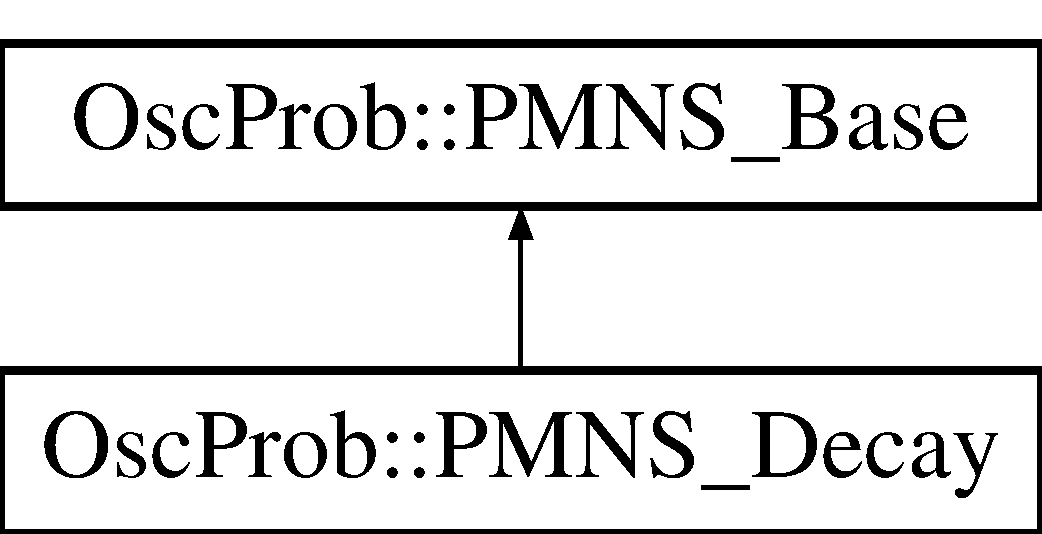
\includegraphics[height=2.000000cm]{classOscProb_1_1PMNS__Decay}
\end{center}
\end{figure}
\subsection*{Public Member Functions}
\begin{DoxyCompactItemize}
\item 
\hyperlink{classOscProb_1_1PMNS__Decay_a866c08feec7ec2cc4b756f327af62635}{P\+M\+N\+S\+\_\+\+Decay} ()
\begin{DoxyCompactList}\small\item\em Constructor. \end{DoxyCompactList}\item 
virtual \hyperlink{classOscProb_1_1PMNS__Decay_ad69de1a9c75af5ec6e3dc52c407b4d85}{$\sim$\+P\+M\+N\+S\+\_\+\+Decay} ()
\begin{DoxyCompactList}\small\item\em Destructor. \end{DoxyCompactList}\item 
virtual void \hyperlink{classOscProb_1_1PMNS__Decay_ab88e15cd257844331f8b54b35ccc7018}{Set\+Mix} (double th12, double th23, double th13, double deltacp)
\begin{DoxyCompactList}\small\item\em Set the all mixing parameters at once. \end{DoxyCompactList}\item 
virtual void \hyperlink{classOscProb_1_1PMNS__Decay_a75b4b57eaefc06f9fbdb662f8772fe96}{Set\+Delta\+Msqrs} (double dm21, double dm32)
\begin{DoxyCompactList}\small\item\em Set both mass-\/splittings at once. \end{DoxyCompactList}\item 
virtual void \hyperlink{classOscProb_1_1PMNS__Decay_a6eed8a6e8ab940a4995d8d2a43ed1307}{Set\+Alpha3} (double alpha3)
\item 
virtual void \hyperlink{classOscProb_1_1PMNS__Decay_a414dd1d7792db6bc52abe9d963148500}{Set\+Alpha2} (double alpha2)
\item 
virtual double \hyperlink{classOscProb_1_1PMNS__Decay_a5a1e1b0cc312c334b22f4efa307d18d8}{Get\+Alpha3} ()
\begin{DoxyCompactList}\small\item\em Get alpha3. \end{DoxyCompactList}\item 
virtual double \hyperlink{classOscProb_1_1PMNS__Decay_a11c0e3144517ad49712d3d3020358149}{Get\+Alpha2} ()
\begin{DoxyCompactList}\small\item\em Get alpha2. \end{DoxyCompactList}\item 
virtual void \hyperlink{classOscProb_1_1PMNS__Decay_a60b2c35652e73d8f6a087f3f2f3c9de6}{Set\+Is\+Nu\+Bar} (bool is\+Nu\+Bar)
\begin{DoxyCompactList}\small\item\em Set the anti-\/neutrino flag. \end{DoxyCompactList}\item 
virtual double \hyperlink{classOscProb_1_1PMNS__Base_aa2e10704d2d205a1ec8988de14b1a66f}{Prob} (std\+::vector$<$ \hyperlink{EigenPoint_8h_a67ca8e107e20610c3fff78d5e726ece0}{complexD} $>$ nu\+\_\+in, int flvf)
\begin{DoxyCompactList}\small\item\em Compute the probability of nu\+\_\+in going to flvf. \end{DoxyCompactList}\item 
virtual double \hyperlink{classOscProb_1_1PMNS__Base_a0190a79284289aacf682c78d7cef9a81}{Prob} (std\+::vector$<$ \hyperlink{EigenPoint_8h_a67ca8e107e20610c3fff78d5e726ece0}{complexD} $>$ nu\+\_\+in, int flvf, double E)
\begin{DoxyCompactList}\small\item\em Compute the probability of nu\+\_\+in going to flvf for energy E. \end{DoxyCompactList}\item 
virtual double \hyperlink{classOscProb_1_1PMNS__Base_a01fba31729345376705e02408e835f67}{Prob} (std\+::vector$<$ \hyperlink{EigenPoint_8h_a67ca8e107e20610c3fff78d5e726ece0}{complexD} $>$ nu\+\_\+in, int flvf, double E, double L)
\begin{DoxyCompactList}\small\item\em Compute the probability of nu\+\_\+in going to flvf for energy E and distance L. \end{DoxyCompactList}\item 
virtual double \hyperlink{classOscProb_1_1PMNS__Base_aec5c399b93261f1962a4b7dbbb44b973}{Prob} (int flvi, int flvf)
\begin{DoxyCompactList}\small\item\em Compute the probability of flvi going to flvf. \end{DoxyCompactList}\item 
virtual double \hyperlink{classOscProb_1_1PMNS__Base_aa3cee10639d5c0879ccb9e78d62128d3}{Prob} (int flvi, int flvf, double E)
\begin{DoxyCompactList}\small\item\em Compute the probability of flvi going to flvf for energy E. \end{DoxyCompactList}\item 
virtual double \hyperlink{classOscProb_1_1PMNS__Base_a6e0a74508d9d6db7be02e242b8467563}{Prob} (int flvi, int flvf, double E, double L)
\begin{DoxyCompactList}\small\item\em Compute the probability of flvi going to flvf for energy E and distance L. \end{DoxyCompactList}\item 
virtual double \hyperlink{classOscProb_1_1PMNS__Base_a89e54c80ae8a31effbab7b2b970606bb}{Avg\+Prob} (std\+::vector$<$ \hyperlink{EigenPoint_8h_a67ca8e107e20610c3fff78d5e726ece0}{complexD} $>$ nu\+\_\+in, int flvf, double E, double dE=0)
\begin{DoxyCompactList}\small\item\em Compute the average probability over a bin of energy. \end{DoxyCompactList}\item 
virtual double \hyperlink{classOscProb_1_1PMNS__Base_ac03f754160422e6600da8dbae0f803ed}{Avg\+Prob} (int flvi, int flvf, double E, double dE=0)
\begin{DoxyCompactList}\small\item\em Compute the average probability over a bin of energy. \end{DoxyCompactList}\item 
virtual double \hyperlink{classOscProb_1_1PMNS__Base_a19f160c045a01e5083506e925fb37d44}{Avg\+Prob\+LoE} (std\+::vector$<$ \hyperlink{EigenPoint_8h_a67ca8e107e20610c3fff78d5e726ece0}{complexD} $>$ nu\+\_\+in, int flvf, double LoE, double d\+LoE=0)
\begin{DoxyCompactList}\small\item\em Compute the average probability over a bin of L/E. \end{DoxyCompactList}\item 
virtual double \hyperlink{classOscProb_1_1PMNS__Base_ac19a92f4ef428a7333ca8eed76fca637}{Avg\+Prob\+LoE} (int flvi, int flvf, double LoE, double d\+LoE=0)
\begin{DoxyCompactList}\small\item\em Compute the average probability over a bin of L/E. \end{DoxyCompactList}\item 
virtual std\+::vector$<$ \hyperlink{EigenPoint_8h_a67ca8e107e20610c3fff78d5e726ece0}{complexD} $>$ \hyperlink{classOscProb_1_1PMNS__Base_a5092561dd8579d390c649eb60803ea98}{Get\+Mass\+Eigenstate} (int mi)
\begin{DoxyCompactList}\small\item\em Get a neutrino mass eigenstate. \end{DoxyCompactList}\item 
virtual void \hyperlink{classOscProb_1_1PMNS__Base_ace7875cf6d3bec161a2b7ed2690aec34}{Set\+Angle} (int i, int j, double th)
\begin{DoxyCompactList}\small\item\em Set the mixing angle theta\+\_\+ij. \end{DoxyCompactList}\item 
virtual void \hyperlink{classOscProb_1_1PMNS__Base_a4bef78cfcfc4e70b4ce79cdb8862c0a3}{Set\+Delta} (int i, int j, double delta)
\begin{DoxyCompactList}\small\item\em Set the CP phase delta\+\_\+ij. \end{DoxyCompactList}\item 
virtual void \hyperlink{classOscProb_1_1PMNS__Base_a492243b22fb1b783cd2943f507cff970}{Set\+Dm} (int j, double dm)
\begin{DoxyCompactList}\small\item\em Set the mass-\/splitting dm\+\_\+j1 in e\+V$^\wedge$2. \end{DoxyCompactList}\item 
virtual double \hyperlink{classOscProb_1_1PMNS__Base_acee137091304c919642293ddf015bbc8}{Get\+Angle} (int i, int j)
\begin{DoxyCompactList}\small\item\em Get the mixing angle theta\+\_\+ij. \end{DoxyCompactList}\item 
virtual double \hyperlink{classOscProb_1_1PMNS__Base_adb8dbc91d4286d2e7c8f768c59476241}{Get\+Delta} (int i, int j)
\begin{DoxyCompactList}\small\item\em Get the CP phase delta\+\_\+ij. \end{DoxyCompactList}\item 
virtual double \hyperlink{classOscProb_1_1PMNS__Base_ad26815ac5f4805d1259817e4936e5f8f}{Get\+Dm} (int j)
\begin{DoxyCompactList}\small\item\em Get the mass-\/splitting dm\+\_\+j1 in e\+V$^\wedge$2. \end{DoxyCompactList}\item 
virtual double \hyperlink{classOscProb_1_1PMNS__Base_a4ea861a6707ce1be3a54aad2b60f8632}{Get\+Dm\+Eff} (int j)
\begin{DoxyCompactList}\small\item\em Get the effective mass-\/splitting dm\+\_\+j1 in e\+V$^\wedge$2. \end{DoxyCompactList}\item 
virtual void \hyperlink{classOscProb_1_1PMNS__Base_a4de96ac9b6d1e9b029ab877e57d211ad}{Set\+Std\+Pars} ()
\begin{DoxyCompactList}\small\item\em Set P\+DG 3-\/flavor parameters. \end{DoxyCompactList}\item 
virtual void \hyperlink{classOscProb_1_1PMNS__Base_a95b3b0d0cab5e6a54b5ef99587f837c0}{Set\+Energy} (double E)
\begin{DoxyCompactList}\small\item\em Set the neutrino energy in GeV. \end{DoxyCompactList}\item 
virtual double \hyperlink{classOscProb_1_1PMNS__Base_acc0d46cc4b8f911b40b807225003bbed}{Get\+Energy} ()
\begin{DoxyCompactList}\small\item\em Get the neutrino energy in GeV. \end{DoxyCompactList}\item 
virtual bool \hyperlink{classOscProb_1_1PMNS__Base_a2f7f2a028dfe7a90fff6b4f757972c2c}{Get\+Is\+Nu\+Bar} ()
\begin{DoxyCompactList}\small\item\em Get the anti-\/neutrino flag. \end{DoxyCompactList}\item 
virtual void \hyperlink{classOscProb_1_1PMNS__Base_ac3b644fd0a56347d304ceca4ae9d8875}{Set\+Path} (\hyperlink{structOscProb_1_1NuPath}{Osc\+Prob\+::\+Nu\+Path} p)
\begin{DoxyCompactList}\small\item\em Set a single path. \end{DoxyCompactList}\item 
virtual void \hyperlink{classOscProb_1_1PMNS__Base_a35b983270613072a3df58b574d80dbfd}{Set\+Path} (double length, double density, double zoa=0.\+5, int layer=0)
\begin{DoxyCompactList}\small\item\em Set a single path. \end{DoxyCompactList}\item 
virtual void \hyperlink{classOscProb_1_1PMNS__Base_a637d19dd850b4246507796526622643c}{Set\+Path} (std\+::vector$<$ \hyperlink{structOscProb_1_1NuPath}{Osc\+Prob\+::\+Nu\+Path} $>$ paths)
\begin{DoxyCompactList}\small\item\em Set a path sequence. \end{DoxyCompactList}\item 
virtual void \hyperlink{classOscProb_1_1PMNS__Base_a887dc9d4dc569ec0cdef3933b4c60efc}{Add\+Path} (\hyperlink{structOscProb_1_1NuPath}{Osc\+Prob\+::\+Nu\+Path} p)
\begin{DoxyCompactList}\small\item\em Add a path to the sequence. \end{DoxyCompactList}\item 
virtual void \hyperlink{classOscProb_1_1PMNS__Base_ab7f89ad9e7e1224adaa59d3c41594cd9}{Add\+Path} (double length, double density, double zoa=0.\+5, int layer=0)
\begin{DoxyCompactList}\small\item\em Add a path to the sequence. \end{DoxyCompactList}\item 
virtual void \hyperlink{classOscProb_1_1PMNS__Base_aefe521239031c418cfaaaa550a6e13bb}{Clear\+Path} ()
\begin{DoxyCompactList}\small\item\em Clear the path vector. \end{DoxyCompactList}\item 
virtual void \hyperlink{classOscProb_1_1PMNS__Base_a6241325b1bd28cafa556daaecbe4ed62}{Set\+Length} (double L)
\begin{DoxyCompactList}\small\item\em Set a single path lentgh in km. \end{DoxyCompactList}\item 
virtual void \hyperlink{classOscProb_1_1PMNS__Base_aa34a40a3b5abda0f252982d9ead3b520}{Set\+Length} (std\+::vector$<$ double $>$ L)
\begin{DoxyCompactList}\small\item\em Set multiple path lengths. \end{DoxyCompactList}\item 
virtual void \hyperlink{classOscProb_1_1PMNS__Base_ac74206f349687da141392c81e2ba6b0d}{Set\+Density} (double rho)
\begin{DoxyCompactList}\small\item\em Set single path density in g/cm$^\wedge$3. \end{DoxyCompactList}\item 
virtual void \hyperlink{classOscProb_1_1PMNS__Base_a858221d5510fe732dc6a101fd305cda0}{Set\+Density} (std\+::vector$<$ double $>$ rho)
\begin{DoxyCompactList}\small\item\em Set multiple path densities. \end{DoxyCompactList}\item 
virtual void \hyperlink{classOscProb_1_1PMNS__Base_a1bf3ea8fd2507fd2fd82d7410ff8f578}{Set\+ZoA} (double zoa)
\begin{DoxyCompactList}\small\item\em Set Z/A value for single path. \end{DoxyCompactList}\item 
virtual void \hyperlink{classOscProb_1_1PMNS__Base_a8495f8a320e1a21965e6a64aec92ad2a}{Set\+ZoA} (std\+::vector$<$ double $>$ zoa)
\begin{DoxyCompactList}\small\item\em Set multiple path Z/A values. \end{DoxyCompactList}\item 
virtual void \hyperlink{classOscProb_1_1PMNS__Base_a904e580edf89fb98bf9a6397739b4ebe}{Set\+Layers} (std\+::vector$<$ int $>$ lay)
\begin{DoxyCompactList}\small\item\em Set multiple path layer indices. \end{DoxyCompactList}\item 
virtual void \hyperlink{classOscProb_1_1PMNS__Base_add6533a9fc9acdfc7ae258b62570d78d}{Set\+Std\+Path} ()
\begin{DoxyCompactList}\small\item\em Set standard neutrino path. \end{DoxyCompactList}\item 
virtual std\+::vector$<$ \hyperlink{structOscProb_1_1NuPath}{Osc\+Prob\+::\+Nu\+Path} $>$ \hyperlink{classOscProb_1_1PMNS__Base_ac8e196f2e85a2b1caaf705073ee95a5c}{Get\+Path} ()
\begin{DoxyCompactList}\small\item\em Get the neutrino path sequence. \end{DoxyCompactList}\item 
virtual std\+::vector$<$ double $>$ \hyperlink{classOscProb_1_1PMNS__Base_a9eac8d768c1424755ee41f7e783af179}{Get\+Sample\+Points} (double LoE, double d\+LoE)
\begin{DoxyCompactList}\small\item\em Compute the sample points for a bin of L/E with width d\+LoE. \end{DoxyCompactList}\item 
virtual void \hyperlink{classOscProb_1_1PMNS__Base_aa94c1e1fff0ba731c75f7e633b023a9f}{Set\+Use\+Cache} (bool u=true)
\begin{DoxyCompactList}\small\item\em Set caching on/off. \end{DoxyCompactList}\item 
virtual void \hyperlink{classOscProb_1_1PMNS__Base_ac47fd33e69aa6490f99e2fd147a92f03}{Clear\+Cache} ()
\begin{DoxyCompactList}\small\item\em Clear the cache. \end{DoxyCompactList}\item 
virtual void \hyperlink{classOscProb_1_1PMNS__Base_ae67862cf58b0802487a14b047b012a78}{Set\+Max\+Cache} (int mc=1e6)
\begin{DoxyCompactList}\small\item\em Set max cache size. \end{DoxyCompactList}\end{DoxyCompactItemize}
\subsection*{Public Attributes}
\begin{DoxyCompactItemize}
\item 
std\+::vector$<$ double $>$ \hyperlink{classOscProb_1_1PMNS__Decay_a0797d1d46ad5eb0b4ce7c3cf8c367713}{falpha}
\item 
std\+::vector$<$ std\+::vector$<$ \hyperlink{EigenPoint_8h_a67ca8e107e20610c3fff78d5e726ece0}{complexD} $>$ $>$ \hyperlink{classOscProb_1_1PMNS__Decay_a519f7489e14237438f54bd82ac150f6a}{f\+Evecinv}
\item 
std\+::vector$<$ double $>$ \hyperlink{classOscProb_1_1PMNS__Decay_a9cc660ef50773b4ae7d3932de47c6473}{f\+EvalI}
\end{DoxyCompactItemize}
\subsection*{Protected Member Functions}
\begin{DoxyCompactItemize}
\item 
virtual void \hyperlink{classOscProb_1_1PMNS__Decay_a002400efd07582713ef788a482771054}{Build\+Ham} ()
\item 
virtual void \hyperlink{classOscProb_1_1PMNS__Decay_a578dfb56b5b238d3e77c7d41b837a6d8}{Update\+Ham} ()
\begin{DoxyCompactList}\small\item\em Build the full Hamiltonian. \end{DoxyCompactList}\item 
virtual void \hyperlink{classOscProb_1_1PMNS__Decay_aab2c974ea66e13233186af8eca319496}{Solve\+Ham} ()
\begin{DoxyCompactList}\small\item\em Solve the full Hamiltonian for eigenvectors and eigenvalues. \end{DoxyCompactList}\item 
virtual void \hyperlink{classOscProb_1_1PMNS__Decay_a12dda597f214e874e958070abc63a37c}{Propagate\+Path} (\hyperlink{structOscProb_1_1NuPath}{Osc\+Prob\+::\+Nu\+Path} p)
\begin{DoxyCompactList}\small\item\em Propagation with D. \end{DoxyCompactList}\item 
virtual void \hyperlink{classOscProb_1_1PMNS__Base_adf23b569112f9f9e0e592f01d79a5f3d}{Initialize\+Vectors} ()
\begin{DoxyCompactList}\small\item\em Initialize all member vectors with zeros. \end{DoxyCompactList}\item 
virtual bool \hyperlink{classOscProb_1_1PMNS__Base_abe533da5f64bec1f4724ab7b58606b77}{Try\+Cache} ()
\begin{DoxyCompactList}\small\item\em Try to find a cached eigensystem. \end{DoxyCompactList}\item 
virtual void \hyperlink{classOscProb_1_1PMNS__Base_a785c37fcea974628623c8881bb0fbbf9}{Fill\+Cache} ()
\begin{DoxyCompactList}\small\item\em Cache the current eigensystem. \end{DoxyCompactList}\item 
virtual void \hyperlink{classOscProb_1_1PMNS__Base_a986e6ebef09a7e2eb7fee16a4c2c834d}{Set\+Cur\+Path} (\hyperlink{structOscProb_1_1NuPath}{Osc\+Prob\+::\+Nu\+Path} p)
\begin{DoxyCompactList}\small\item\em Set the path currently in use by the class. \end{DoxyCompactList}\item 
virtual void \hyperlink{classOscProb_1_1PMNS__Base_aba565962a440d14bee7a2a96d2eca2c5}{Set\+Att} (double att, int idx)
\begin{DoxyCompactList}\small\item\em Set one of the path attributes. \end{DoxyCompactList}\item 
virtual void \hyperlink{classOscProb_1_1PMNS__Base_aa001479b5f5828c3d16ed087f96ecbcc}{Set\+Att} (std\+::vector$<$ double $>$ att, int idx)
\begin{DoxyCompactList}\small\item\em Set all values of a path attribute. \end{DoxyCompactList}\item 
virtual void \hyperlink{classOscProb_1_1PMNS__Base_a6a3cf45bbe2349abf06708b65677c044}{RotateH} (int i, int j, std\+::vector$<$ std\+::vector$<$ \hyperlink{EigenPoint_8h_a67ca8e107e20610c3fff78d5e726ece0}{complexD} $>$ $>$ \&Ham)
\begin{DoxyCompactList}\small\item\em Rotate the Hamiltonian by theta\+\_\+ij and delta\+\_\+ij. \end{DoxyCompactList}\item 
virtual void \hyperlink{classOscProb_1_1PMNS__Base_ae52554477ad3250daa5adb8c32cab0b4}{Rotate\+State} (int i, int j)
\begin{DoxyCompactList}\small\item\em Rotate the neutrino state by theta\+\_\+ij and delta\+\_\+ij. \end{DoxyCompactList}\item 
virtual void \hyperlink{classOscProb_1_1PMNS__Base_ad0faf5eae755afb1baa1fcd5ffebad41}{Build\+Hms} ()
\begin{DoxyCompactList}\small\item\em Build the matrix of masses squared. \end{DoxyCompactList}\item 
virtual void \hyperlink{classOscProb_1_1PMNS__Base_ac0d4bf8ff1318ef96d3dafa62e0cec25}{Reset\+To\+Flavour} (int flv)
\begin{DoxyCompactList}\small\item\em Reset neutrino state to pure flavour flv. \end{DoxyCompactList}\item 
virtual void \hyperlink{classOscProb_1_1PMNS__Base_a054e3a8b05b9a958b6fa416e4a835e3e}{Propagate} ()
\begin{DoxyCompactList}\small\item\em Propagate neutrino through full path. \end{DoxyCompactList}\item 
virtual double \hyperlink{classOscProb_1_1PMNS__Base_a0dc4d45bc3d7e03b9abbf5b4e100cc22}{P} (int flv)
\begin{DoxyCompactList}\small\item\em Return the probability of final state in flavour flv. \end{DoxyCompactList}\end{DoxyCompactItemize}
\subsection*{Protected Attributes}
\begin{DoxyCompactItemize}
\item 
std\+::vector$<$ std\+::vector$<$ \hyperlink{EigenPoint_8h_a67ca8e107e20610c3fff78d5e726ece0}{complexD} $>$ $>$ \hyperlink{classOscProb_1_1PMNS__Decay_a77801524bbf55b187ffad7992194d474}{f\+Hd}
\item 
std\+::vector$<$ std\+::vector$<$ \hyperlink{EigenPoint_8h_a67ca8e107e20610c3fff78d5e726ece0}{complexD} $>$ $>$ \hyperlink{classOscProb_1_1PMNS__Decay_aebc95f5c0de55caa8dfb8c1b175e4343}{f\+Ham}
\item 
std\+::vector$<$ std\+::vector$<$ \hyperlink{EigenPoint_8h_a67ca8e107e20610c3fff78d5e726ece0}{complexD} $>$ $>$ \hyperlink{classOscProb_1_1PMNS__Decay_aabd3996c0e09bf3673e0453328d247b0}{f\+Ht}
\item 
std\+::vector$<$ \hyperlink{EigenPoint_8h_a67ca8e107e20610c3fff78d5e726ece0}{complexD} $>$ \hyperlink{classOscProb_1_1PMNS__Decay_a0cc6c8e380edb7a0bb55556805e4e7ff}{f\+Eval\+Eigen}
\item 
std\+::vector$<$ std\+::vector$<$ \hyperlink{EigenPoint_8h_a67ca8e107e20610c3fff78d5e726ece0}{complexD} $>$ $>$ \hyperlink{classOscProb_1_1PMNS__Decay_a2e3b50763e255a0592fd5e099129c367}{f\+Evec\+Eigen}
\item 
std\+::vector$<$ std\+::vector$<$ \hyperlink{EigenPoint_8h_a67ca8e107e20610c3fff78d5e726ece0}{complexD} $>$ $>$ \hyperlink{classOscProb_1_1PMNS__Decay_ab6ea0333a390cb35a2a2d24b2d5fc3dd}{f\+Evec\+Eigeninv}
\item 
int \hyperlink{classOscProb_1_1PMNS__Base_a24bb74bed63569dfe88b18fa6a08060e}{f\+Num\+Nus}
\begin{DoxyCompactList}\small\item\em Number of neutrino flavours. \end{DoxyCompactList}\item 
std\+::vector$<$ double $>$ \hyperlink{classOscProb_1_1PMNS__Base_a406a31c3b5d620e5a0cace5b411f9f70}{f\+Dm}
\begin{DoxyCompactList}\small\item\em m$^\wedge$2\+\_\+i -\/ m$^\wedge$2\+\_\+1 in vacuum \end{DoxyCompactList}\item 
std\+::vector$<$ std\+::vector$<$ double $>$ $>$ \hyperlink{classOscProb_1_1PMNS__Base_a1976887cd658dd86b2336c181f1470b4}{f\+Theta}
\begin{DoxyCompactList}\small\item\em theta\mbox{[}i\mbox{]}\mbox{[}j\mbox{]} mixing angle \end{DoxyCompactList}\item 
std\+::vector$<$ std\+::vector$<$ double $>$ $>$ \hyperlink{classOscProb_1_1PMNS__Base_ab2a5fa40e689b221c8a7d2c17213810d}{f\+Delta}
\begin{DoxyCompactList}\small\item\em delta\mbox{[}i\mbox{]}\mbox{[}j\mbox{]} CP violating phase \end{DoxyCompactList}\item 
std\+::vector$<$ \hyperlink{EigenPoint_8h_a67ca8e107e20610c3fff78d5e726ece0}{complexD} $>$ \hyperlink{classOscProb_1_1PMNS__Base_abf99f2339e3ee989600740b5d88063e8}{f\+Nu\+State}
\begin{DoxyCompactList}\small\item\em The neutrino current state. \end{DoxyCompactList}\item 
std\+::vector$<$ std\+::vector$<$ \hyperlink{EigenPoint_8h_a67ca8e107e20610c3fff78d5e726ece0}{complexD} $>$ $>$ \hyperlink{classOscProb_1_1PMNS__Base_acd3c8783e7603081eab316ea4c86c766}{f\+Hms}
\begin{DoxyCompactList}\small\item\em matrix H$\ast$2E in e\+V$^\wedge$2 \end{DoxyCompactList}\item 
std\+::vector$<$ \hyperlink{EigenPoint_8h_a67ca8e107e20610c3fff78d5e726ece0}{complexD} $>$ \hyperlink{classOscProb_1_1PMNS__Base_ab8d26b722047d49d977f5f2d83026ede}{f\+Phases}
\begin{DoxyCompactList}\small\item\em Buffer for oscillation phases. \end{DoxyCompactList}\item 
std\+::vector$<$ \hyperlink{EigenPoint_8h_a67ca8e107e20610c3fff78d5e726ece0}{complexD} $>$ \hyperlink{classOscProb_1_1PMNS__Base_a5440bc3efa466a37649601abce559e3e}{f\+Buffer}
\begin{DoxyCompactList}\small\item\em Buffer for neutrino state tranformations. \end{DoxyCompactList}\item 
std\+::vector$<$ double $>$ \hyperlink{classOscProb_1_1PMNS__Base_a6319c34d7decbb9d7d6da279c06e8c2d}{f\+Eval}
\begin{DoxyCompactList}\small\item\em Eigenvalues of the Hamiltonian. \end{DoxyCompactList}\item 
std\+::vector$<$ std\+::vector$<$ \hyperlink{EigenPoint_8h_a67ca8e107e20610c3fff78d5e726ece0}{complexD} $>$ $>$ \hyperlink{classOscProb_1_1PMNS__Base_a87be137356c5f27ab83cab5e1298ef8f}{f\+Evec}
\begin{DoxyCompactList}\small\item\em Eigenvectors of the Hamiltonian. \end{DoxyCompactList}\item 
double \hyperlink{classOscProb_1_1PMNS__Base_a2800af6d436972f3e900867790c046b0}{f\+Energy}
\begin{DoxyCompactList}\small\item\em Neutrino energy. \end{DoxyCompactList}\item 
bool \hyperlink{classOscProb_1_1PMNS__Base_a0ebaeaefab36a3ff381c6293faedfdd6}{f\+Is\+Nu\+Bar}
\begin{DoxyCompactList}\small\item\em Anti-\/neutrino flag. \end{DoxyCompactList}\item 
std\+::vector$<$ \hyperlink{structOscProb_1_1NuPath}{Osc\+Prob\+::\+Nu\+Path} $>$ \hyperlink{classOscProb_1_1PMNS__Base_a69db9d57e12fc7cbe0431bc6c18fac93}{f\+Nu\+Paths}
\begin{DoxyCompactList}\small\item\em Vector of neutrino paths. \end{DoxyCompactList}\item 
\hyperlink{structOscProb_1_1NuPath}{Osc\+Prob\+::\+Nu\+Path} \hyperlink{classOscProb_1_1PMNS__Base_a849437aa8891fe042e86886ce8f81c6e}{f\+Path}
\begin{DoxyCompactList}\small\item\em Current neutrino path. \end{DoxyCompactList}\item 
bool \hyperlink{classOscProb_1_1PMNS__Base_a9ac3cadeac8db1b90f3152f476244780}{f\+Built\+Hms}
\begin{DoxyCompactList}\small\item\em Tag to avoid rebuilding Hms. \end{DoxyCompactList}\item 
bool \hyperlink{classOscProb_1_1PMNS__Base_a6dc5cd010d2d70b2324745b4e53e9839}{f\+Got\+ES}
\begin{DoxyCompactList}\small\item\em Tag to avoid recalculating eigensystem. \end{DoxyCompactList}\item 
bool \hyperlink{classOscProb_1_1PMNS__Base_ad28c12ef897b5555eda509ea55c99107}{f\+Use\+Cache}
\begin{DoxyCompactList}\small\item\em Flag for whether to use caching. \end{DoxyCompactList}\item 
double \hyperlink{classOscProb_1_1PMNS__Base_a0b4c41a27de281472453a1912cbc1e64}{f\+Cache\+Prec}
\begin{DoxyCompactList}\small\item\em Precision of cache matching. \end{DoxyCompactList}\item 
int \hyperlink{classOscProb_1_1PMNS__Base_a74c13356eafec2490d8c3c19759ba7f0}{f\+Max\+Cache}
\begin{DoxyCompactList}\small\item\em Maximum cache size. \end{DoxyCompactList}\item 
std\+::set$<$ \hyperlink{structOscProb_1_1EigenPoint}{Osc\+Prob\+::\+Eigen\+Point} $>$ \hyperlink{classOscProb_1_1PMNS__Base_a8159424f20197a3a7145fe3bf2c11176}{f\+Mix\+Cache}
\begin{DoxyCompactList}\small\item\em Caching set of eigensystems. \end{DoxyCompactList}\item 
\hyperlink{structOscProb_1_1EigenPoint}{Eigen\+Point} \hyperlink{classOscProb_1_1PMNS__Base_ab1fe4800ee3ae48df4fc942dce00e0d3}{f\+Probe}
\begin{DoxyCompactList}\small\item\em Eigenp\+Point to try. \end{DoxyCompactList}\end{DoxyCompactItemize}
\subsection*{Static Protected Attributes}
\begin{DoxyCompactItemize}
\item 
static const \hyperlink{EigenPoint_8h_a67ca8e107e20610c3fff78d5e726ece0}{complexD} \hyperlink{classOscProb_1_1PMNS__Base_a05e595848c2521dc795efa7645728b94}{zero}
\begin{DoxyCompactList}\small\item\em zero in complex \end{DoxyCompactList}\item 
static const \hyperlink{EigenPoint_8h_a67ca8e107e20610c3fff78d5e726ece0}{complexD} \hyperlink{classOscProb_1_1PMNS__Base_a7d1d0bbcab30a1fd8c368c40134c51ff}{one}
\begin{DoxyCompactList}\small\item\em one in complex \end{DoxyCompactList}\item 
static const double \hyperlink{classOscProb_1_1PMNS__Base_a382ddd7b76ca89b43f22614a2ea7327b}{k\+Km2eV} = 1.\+0 / 1.\+973269788e-\/10
\begin{DoxyCompactList}\small\item\em km to e\+V$^\wedge$-\/1 \end{DoxyCompactList}\item 
static const double \hyperlink{classOscProb_1_1PMNS__Base_a326fc5016d7dd7ce05682c06cdcb6d94}{k\+K2} = 1e-\/3 $\ast$ k\+N\+A / pow(k\+Km2e\+V,3)
\begin{DoxyCompactList}\small\item\em mol/\+Ge\+V$^\wedge$2/cm$^\wedge$3 to eV \end{DoxyCompactList}\item 
static const double \hyperlink{classOscProb_1_1PMNS__Base_ad36a0a6bf58d6ec093d3947784bd89e9}{k\+Ge\+V2eV} = 1.\+0e+09
\begin{DoxyCompactList}\small\item\em GeV to eV. \end{DoxyCompactList}\item 
static const double \hyperlink{classOscProb_1_1PMNS__Base_a69355e770b89e99437c2b8a66e48eeb9}{k\+NA} = 6.\+022140857e23
\begin{DoxyCompactList}\small\item\em Avogadro constant. \end{DoxyCompactList}\item 
static const double \hyperlink{classOscProb_1_1PMNS__Base_a7f26a3456128234b2ae6cc9141a6532f}{k\+Gf} = 1.\+1663787e-\/05
\begin{DoxyCompactList}\small\item\em G\+\_\+F in units of Ge\+V$^\wedge$-\/2. \end{DoxyCompactList}\end{DoxyCompactItemize}


\subsection{Detailed Description}
......................................................................

\begin{DoxyAuthor}{Author}
Victor Carretero -\/ \href{mailto:vcarretero@km3net.de}{\tt vcarretero@km3net.\+de} 
\end{DoxyAuthor}


Definition at line 21 of file P\+M\+N\+S\+\_\+\+Decay.\+h.



\subsection{Constructor \& Destructor Documentation}
\mbox{\Hypertarget{classOscProb_1_1PMNS__Decay_a866c08feec7ec2cc4b756f327af62635}\label{classOscProb_1_1PMNS__Decay_a866c08feec7ec2cc4b756f327af62635}} 
\index{Osc\+Prob\+::\+P\+M\+N\+S\+\_\+\+Decay@{Osc\+Prob\+::\+P\+M\+N\+S\+\_\+\+Decay}!P\+M\+N\+S\+\_\+\+Decay@{P\+M\+N\+S\+\_\+\+Decay}}
\index{P\+M\+N\+S\+\_\+\+Decay@{P\+M\+N\+S\+\_\+\+Decay}!Osc\+Prob\+::\+P\+M\+N\+S\+\_\+\+Decay@{Osc\+Prob\+::\+P\+M\+N\+S\+\_\+\+Decay}}
\subsubsection{\texorpdfstring{P\+M\+N\+S\+\_\+\+Decay()}{PMNS\_Decay()}}
{\footnotesize\ttfamily P\+M\+N\+S\+\_\+\+Decay\+::\+P\+M\+N\+S\+\_\+\+Decay (\begin{DoxyParamCaption}{ }\end{DoxyParamCaption})}

Constructor. \begin{DoxySeeAlso}{See also}
\hyperlink{classOscProb_1_1PMNS__Base_aa53e83b03a9cf4bdfa0a07136bd17a79}{P\+M\+N\+S\+\_\+\+Base\+::\+P\+M\+N\+S\+\_\+\+Base}
\end{DoxySeeAlso}
This class is restricted to 3 neutrino flavours. 

Definition at line 30 of file P\+M\+N\+S\+\_\+\+Decay.\+cxx.



References falpha, f\+Eval\+Eigen, f\+EvalI, f\+Evec\+Eigen, f\+Evec\+Eigeninv, f\+Evecinv, f\+Ham, f\+Hd, f\+Ht, Osc\+Prob\+::\+P\+M\+N\+S\+\_\+\+Base\+::f\+Num\+Nus, and Osc\+Prob\+::\+P\+M\+N\+S\+\_\+\+Base\+::zero.


\begin{DoxyCode}
30                        : \hyperlink{classOscProb_1_1PMNS__Base_aa53e83b03a9cf4bdfa0a07136bd17a79}{PMNS\_Base}(), \hyperlink{classOscProb_1_1PMNS__Decay_aebc95f5c0de55caa8dfb8c1b175e4343}{fHam}() \{
31         \hyperlink{classOscProb_1_1PMNS__Decay_a0797d1d46ad5eb0b4ce7c3cf8c367713}{falpha}         = vector<double>(\hyperlink{classOscProb_1_1PMNS__Base_a24bb74bed63569dfe88b18fa6a08060e}{fNumNus}, 0);
32         \hyperlink{classOscProb_1_1PMNS__Decay_a9cc660ef50773b4ae7d3932de47c6473}{fEvalI}         = vector<double>(\hyperlink{classOscProb_1_1PMNS__Base_a24bb74bed63569dfe88b18fa6a08060e}{fNumNus}, 0); 
33         \hyperlink{classOscProb_1_1PMNS__Decay_a519f7489e14237438f54bd82ac150f6a}{fEvecinv}       = vector< vector<complexD> >(\hyperlink{classOscProb_1_1PMNS__Base_a24bb74bed63569dfe88b18fa6a08060e}{fNumNus}, vector<complexD>(
      \hyperlink{classOscProb_1_1PMNS__Base_a24bb74bed63569dfe88b18fa6a08060e}{fNumNus},\hyperlink{classOscProb_1_1PMNS__Base_a05e595848c2521dc795efa7645728b94}{zero}));
34         \hyperlink{classOscProb_1_1PMNS__Decay_a0cc6c8e380edb7a0bb55556805e4e7ff}{fEvalEigen}     = vector<complexD>(\hyperlink{classOscProb_1_1PMNS__Base_a24bb74bed63569dfe88b18fa6a08060e}{fNumNus}, 0);
35         \hyperlink{classOscProb_1_1PMNS__Decay_a2e3b50763e255a0592fd5e099129c367}{fEvecEigen}     = vector< vector<complexD> >(\hyperlink{classOscProb_1_1PMNS__Base_a24bb74bed63569dfe88b18fa6a08060e}{fNumNus}, vector<complexD>(
      \hyperlink{classOscProb_1_1PMNS__Base_a24bb74bed63569dfe88b18fa6a08060e}{fNumNus},\hyperlink{classOscProb_1_1PMNS__Base_a05e595848c2521dc795efa7645728b94}{zero}));
36         \hyperlink{classOscProb_1_1PMNS__Decay_ab6ea0333a390cb35a2a2d24b2d5fc3dd}{fEvecEigeninv}  = vector< vector<complexD> >(\hyperlink{classOscProb_1_1PMNS__Base_a24bb74bed63569dfe88b18fa6a08060e}{fNumNus}, vector<complexD>(
      \hyperlink{classOscProb_1_1PMNS__Base_a24bb74bed63569dfe88b18fa6a08060e}{fNumNus},\hyperlink{classOscProb_1_1PMNS__Base_a05e595848c2521dc795efa7645728b94}{zero}));
37         \hyperlink{classOscProb_1_1PMNS__Decay_a77801524bbf55b187ffad7992194d474}{fHd}            = vector< vector<complexD> >(\hyperlink{classOscProb_1_1PMNS__Base_a24bb74bed63569dfe88b18fa6a08060e}{fNumNus}, vector<complexD>(
      \hyperlink{classOscProb_1_1PMNS__Base_a24bb74bed63569dfe88b18fa6a08060e}{fNumNus},\hyperlink{classOscProb_1_1PMNS__Base_a05e595848c2521dc795efa7645728b94}{zero}));       
38         \hyperlink{classOscProb_1_1PMNS__Decay_aebc95f5c0de55caa8dfb8c1b175e4343}{fHam}           = vector< vector<complexD> >(\hyperlink{classOscProb_1_1PMNS__Base_a24bb74bed63569dfe88b18fa6a08060e}{fNumNus}, vector<complexD>(
      \hyperlink{classOscProb_1_1PMNS__Base_a24bb74bed63569dfe88b18fa6a08060e}{fNumNus},\hyperlink{classOscProb_1_1PMNS__Base_a05e595848c2521dc795efa7645728b94}{zero}));
39         \hyperlink{classOscProb_1_1PMNS__Decay_aabd3996c0e09bf3673e0453328d247b0}{fHt}            = vector< vector<complexD> >(\hyperlink{classOscProb_1_1PMNS__Base_a24bb74bed63569dfe88b18fa6a08060e}{fNumNus}, vector<complexD>(
      \hyperlink{classOscProb_1_1PMNS__Base_a24bb74bed63569dfe88b18fa6a08060e}{fNumNus},\hyperlink{classOscProb_1_1PMNS__Base_a05e595848c2521dc795efa7645728b94}{zero}));
40         \}
\end{DoxyCode}
\mbox{\Hypertarget{classOscProb_1_1PMNS__Decay_ad69de1a9c75af5ec6e3dc52c407b4d85}\label{classOscProb_1_1PMNS__Decay_ad69de1a9c75af5ec6e3dc52c407b4d85}} 
\index{Osc\+Prob\+::\+P\+M\+N\+S\+\_\+\+Decay@{Osc\+Prob\+::\+P\+M\+N\+S\+\_\+\+Decay}!````~P\+M\+N\+S\+\_\+\+Decay@{$\sim$\+P\+M\+N\+S\+\_\+\+Decay}}
\index{````~P\+M\+N\+S\+\_\+\+Decay@{$\sim$\+P\+M\+N\+S\+\_\+\+Decay}!Osc\+Prob\+::\+P\+M\+N\+S\+\_\+\+Decay@{Osc\+Prob\+::\+P\+M\+N\+S\+\_\+\+Decay}}
\subsubsection{\texorpdfstring{$\sim$\+P\+M\+N\+S\+\_\+\+Decay()}{~PMNS\_Decay()}}
{\footnotesize\ttfamily P\+M\+N\+S\+\_\+\+Decay\+::$\sim$\+P\+M\+N\+S\+\_\+\+Decay (\begin{DoxyParamCaption}{ }\end{DoxyParamCaption})\hspace{0.3cm}{\ttfamily [virtual]}}

Nothing to clean. 

Definition at line 46 of file P\+M\+N\+S\+\_\+\+Decay.\+cxx.


\begin{DoxyCode}
46 \{\}
\end{DoxyCode}


\subsection{Member Function Documentation}
\mbox{\Hypertarget{classOscProb_1_1PMNS__Base_a887dc9d4dc569ec0cdef3933b4c60efc}\label{classOscProb_1_1PMNS__Base_a887dc9d4dc569ec0cdef3933b4c60efc}} 
\index{Osc\+Prob\+::\+P\+M\+N\+S\+\_\+\+Decay@{Osc\+Prob\+::\+P\+M\+N\+S\+\_\+\+Decay}!Add\+Path@{Add\+Path}}
\index{Add\+Path@{Add\+Path}!Osc\+Prob\+::\+P\+M\+N\+S\+\_\+\+Decay@{Osc\+Prob\+::\+P\+M\+N\+S\+\_\+\+Decay}}
\subsubsection{\texorpdfstring{Add\+Path()}{AddPath()}\hspace{0.1cm}{\footnotesize\ttfamily [1/2]}}
{\footnotesize\ttfamily void P\+M\+N\+S\+\_\+\+Base\+::\+Add\+Path (\begin{DoxyParamCaption}\item[{\hyperlink{structOscProb_1_1NuPath}{Osc\+Prob\+::\+Nu\+Path}}]{p }\end{DoxyParamCaption})\hspace{0.3cm}{\ttfamily [virtual]}, {\ttfamily [inherited]}}

Add a path to the sequence. 
\begin{DoxyParams}{Parameters}
{\em p} & -\/ A neutrino path segment \\
\hline
\end{DoxyParams}


Definition at line 351 of file P\+M\+N\+S\+\_\+\+Base.\+cxx.



References Osc\+Prob\+::\+P\+M\+N\+S\+\_\+\+Base\+::f\+Nu\+Paths.



Referenced by Osc\+Prob\+::\+P\+M\+N\+S\+\_\+\+Base\+::\+Add\+Path(), Osc\+Prob\+::\+P\+M\+N\+S\+\_\+\+Base\+::\+Set\+Att(), and Osc\+Prob\+::\+P\+M\+N\+S\+\_\+\+Base\+::\+Set\+Path().


\begin{DoxyCode}
351                                \{
352 
353   \hyperlink{classOscProb_1_1PMNS__Base_a69db9d57e12fc7cbe0431bc6c18fac93}{fNuPaths}.push\_back(p);
354 
355 \}
\end{DoxyCode}
\mbox{\Hypertarget{classOscProb_1_1PMNS__Base_ab7f89ad9e7e1224adaa59d3c41594cd9}\label{classOscProb_1_1PMNS__Base_ab7f89ad9e7e1224adaa59d3c41594cd9}} 
\index{Osc\+Prob\+::\+P\+M\+N\+S\+\_\+\+Decay@{Osc\+Prob\+::\+P\+M\+N\+S\+\_\+\+Decay}!Add\+Path@{Add\+Path}}
\index{Add\+Path@{Add\+Path}!Osc\+Prob\+::\+P\+M\+N\+S\+\_\+\+Decay@{Osc\+Prob\+::\+P\+M\+N\+S\+\_\+\+Decay}}
\subsubsection{\texorpdfstring{Add\+Path()}{AddPath()}\hspace{0.1cm}{\footnotesize\ttfamily [2/2]}}
{\footnotesize\ttfamily void P\+M\+N\+S\+\_\+\+Base\+::\+Add\+Path (\begin{DoxyParamCaption}\item[{double}]{length,  }\item[{double}]{density,  }\item[{double}]{zoa = {\ttfamily 0.5},  }\item[{int}]{layer = {\ttfamily 0} }\end{DoxyParamCaption})\hspace{0.3cm}{\ttfamily [virtual]}, {\ttfamily [inherited]}}

Add a path to the sequence defining attributes directly. 
\begin{DoxyParams}{Parameters}
{\em length} & -\/ The length of the path segment in km \\
\hline
{\em density} & -\/ The density of the path segment in g/cm$^\wedge$3 \\
\hline
{\em zoa} & -\/ The effective Z/A of the path segment \\
\hline
{\em layer} & -\/ An index to identify the layer type (e.\+g. earth inner core) \\
\hline
\end{DoxyParams}


Definition at line 365 of file P\+M\+N\+S\+\_\+\+Base.\+cxx.



References Osc\+Prob\+::\+P\+M\+N\+S\+\_\+\+Base\+::\+Add\+Path().


\begin{DoxyCode}
365                                                                            \{
366 
367   \hyperlink{classOscProb_1_1PMNS__Base_a887dc9d4dc569ec0cdef3933b4c60efc}{AddPath}(\hyperlink{structOscProb_1_1NuPath}{NuPath}(length, density, zoa, layer));
368 
369 \}
\end{DoxyCode}
\mbox{\Hypertarget{classOscProb_1_1PMNS__Base_a89e54c80ae8a31effbab7b2b970606bb}\label{classOscProb_1_1PMNS__Base_a89e54c80ae8a31effbab7b2b970606bb}} 
\index{Osc\+Prob\+::\+P\+M\+N\+S\+\_\+\+Decay@{Osc\+Prob\+::\+P\+M\+N\+S\+\_\+\+Decay}!Avg\+Prob@{Avg\+Prob}}
\index{Avg\+Prob@{Avg\+Prob}!Osc\+Prob\+::\+P\+M\+N\+S\+\_\+\+Decay@{Osc\+Prob\+::\+P\+M\+N\+S\+\_\+\+Decay}}
\subsubsection{\texorpdfstring{Avg\+Prob()}{AvgProb()}\hspace{0.1cm}{\footnotesize\ttfamily [1/2]}}
{\footnotesize\ttfamily double P\+M\+N\+S\+\_\+\+Base\+::\+Avg\+Prob (\begin{DoxyParamCaption}\item[{std\+::vector$<$ \hyperlink{EigenPoint_8h_a67ca8e107e20610c3fff78d5e726ece0}{complexD} $>$}]{nu\+\_\+in,  }\item[{int}]{flvf,  }\item[{double}]{E,  }\item[{double}]{dE = {\ttfamily 0} }\end{DoxyParamCaption})\hspace{0.3cm}{\ttfamily [virtual]}, {\ttfamily [inherited]}}

Compute the average probability of nu\+\_\+in going to flvf over a bin of energy E with width dE.

This gets transformed into L/E, since the oscillation terms have arguments linear in L/E and not E.

This function works best for single paths. In multiple paths the accuracy may be somewhat worse. If needed, average over smaller energy ranges.

Flavours are\+: 
\begin{DoxyPre}
  0 = nue, 1 = numu, 2 = nutau
  3 = sterile\_1, 4 = sterile\_2, etc.
\end{DoxyPre}
 
\begin{DoxyParams}{Parameters}
{\em nu\+\_\+in} & -\/ The neutrino initial state in flavour. \\
\hline
{\em flvf} & -\/ The neutrino final flavour. \\
\hline
{\em E} & -\/ The neutrino energy in the bin center in GeV \\
\hline
{\em dE} & -\/ The energy bin width in GeV\\
\hline
\end{DoxyParams}
\begin{DoxyReturn}{Returns}
Average neutrino oscillation probability 
\end{DoxyReturn}


Definition at line 1386 of file P\+M\+N\+S\+\_\+\+Base.\+cxx.



References Osc\+Prob\+::\+Avg\+Path(), Osc\+Prob\+::\+P\+M\+N\+S\+\_\+\+Base\+::\+Avg\+Prob\+Lo\+E(), Osc\+Prob\+::\+P\+M\+N\+S\+\_\+\+Base\+::f\+Nu\+Paths, Osc\+Prob\+::\+P\+M\+N\+S\+\_\+\+Base\+::f\+Path, Osc\+Prob\+::\+Nu\+Path\+::length, Osc\+Prob\+::\+P\+M\+N\+S\+\_\+\+Base\+::\+Prob(), and Osc\+Prob\+::\+P\+M\+N\+S\+\_\+\+Base\+::\+Set\+Cur\+Path().



Referenced by Osc\+Prob\+::\+P\+M\+N\+S\+\_\+\+Base\+::\+Avg\+Prob().


\begin{DoxyCode}
1387 \{
1388 
1389   \textcolor{comment}{// Do nothing if energy is not positive}
1390   \textcolor{keywordflow}{if}(E<=0) \textcolor{keywordflow}{return} 0;
1391 
1392   \textcolor{keywordflow}{if}(\hyperlink{classOscProb_1_1PMNS__Base_a69db9d57e12fc7cbe0431bc6c18fac93}{fNuPaths}.empty()) \textcolor{keywordflow}{return} 0;
1393 
1394   \textcolor{comment}{// Don't average zero width}
1395   \textcolor{keywordflow}{if}(dE<=0) \textcolor{keywordflow}{return} \hyperlink{classOscProb_1_1PMNS__Base_aa2e10704d2d205a1ec8988de14b1a66f}{Prob}(nu\_in, flvf, E);
1396 
1397   \textcolor{comment}{// Make sure fPath is set}
1398   \textcolor{comment}{// Use average if multiple paths}
1399   \hyperlink{classOscProb_1_1PMNS__Base_a986e6ebef09a7e2eb7fee16a4c2c834d}{SetCurPath}(\hyperlink{namespaceOscProb_a999a7944bad8bc72d7ee9f56f81a210e}{AvgPath}(\hyperlink{classOscProb_1_1PMNS__Base_a69db9d57e12fc7cbe0431bc6c18fac93}{fNuPaths}));
1400 
1401   \textcolor{comment}{// Define L/E variables}
1402   \textcolor{keywordtype}{double} LoE = 0;
1403   \textcolor{keywordtype}{double} dLoE = 0;
1404 
1405   \textcolor{comment}{// Set a minimum energy}
1406   \textcolor{keywordtype}{double} minE = 0.1 * E;
1407 
1408   \textcolor{comment}{// Transform range to L/E}
1409   \textcolor{comment}{// Full range if low edge > minE}
1410   \textcolor{keywordflow}{if}(E-dE/2 > minE)\{
1411     LoE = 0.5 * (\hyperlink{classOscProb_1_1PMNS__Base_a849437aa8891fe042e86886ce8f81c6e}{fPath}.\hyperlink{structOscProb_1_1NuPath_af22660894b6e25cf835500381b155557}{length}/(E-dE/2) + \hyperlink{classOscProb_1_1PMNS__Base_a849437aa8891fe042e86886ce8f81c6e}{fPath}.\hyperlink{structOscProb_1_1NuPath_af22660894b6e25cf835500381b155557}{length}/(E+dE/2));
1412     dLoE = \hyperlink{classOscProb_1_1PMNS__Base_a849437aa8891fe042e86886ce8f81c6e}{fPath}.\hyperlink{structOscProb_1_1NuPath_af22660894b6e25cf835500381b155557}{length}/(E-dE/2) - \hyperlink{classOscProb_1_1PMNS__Base_a849437aa8891fe042e86886ce8f81c6e}{fPath}.\hyperlink{structOscProb_1_1NuPath_af22660894b6e25cf835500381b155557}{length}/(E+dE/2);
1413   \}
1414   \textcolor{comment}{// Else start at minE}
1415   \textcolor{keywordflow}{else}\{
1416     LoE = 0.5 * (\hyperlink{classOscProb_1_1PMNS__Base_a849437aa8891fe042e86886ce8f81c6e}{fPath}.\hyperlink{structOscProb_1_1NuPath_af22660894b6e25cf835500381b155557}{length}/minE + \hyperlink{classOscProb_1_1PMNS__Base_a849437aa8891fe042e86886ce8f81c6e}{fPath}.\hyperlink{structOscProb_1_1NuPath_af22660894b6e25cf835500381b155557}{length}/(E+dE/2));
1417     dLoE = \hyperlink{classOscProb_1_1PMNS__Base_a849437aa8891fe042e86886ce8f81c6e}{fPath}.\hyperlink{structOscProb_1_1NuPath_af22660894b6e25cf835500381b155557}{length}/minE - \hyperlink{classOscProb_1_1PMNS__Base_a849437aa8891fe042e86886ce8f81c6e}{fPath}.\hyperlink{structOscProb_1_1NuPath_af22660894b6e25cf835500381b155557}{length}/(E+dE/2);
1418   \}
1419 
1420   \textcolor{comment}{// Compute average in LoE}
1421   \textcolor{keywordflow}{return} \hyperlink{classOscProb_1_1PMNS__Base_a19f160c045a01e5083506e925fb37d44}{AvgProbLoE}(nu\_in, flvf, LoE, dLoE);
1422 
1423 \}
\end{DoxyCode}
\mbox{\Hypertarget{classOscProb_1_1PMNS__Base_ac03f754160422e6600da8dbae0f803ed}\label{classOscProb_1_1PMNS__Base_ac03f754160422e6600da8dbae0f803ed}} 
\index{Osc\+Prob\+::\+P\+M\+N\+S\+\_\+\+Decay@{Osc\+Prob\+::\+P\+M\+N\+S\+\_\+\+Decay}!Avg\+Prob@{Avg\+Prob}}
\index{Avg\+Prob@{Avg\+Prob}!Osc\+Prob\+::\+P\+M\+N\+S\+\_\+\+Decay@{Osc\+Prob\+::\+P\+M\+N\+S\+\_\+\+Decay}}
\subsubsection{\texorpdfstring{Avg\+Prob()}{AvgProb()}\hspace{0.1cm}{\footnotesize\ttfamily [2/2]}}
{\footnotesize\ttfamily double P\+M\+N\+S\+\_\+\+Base\+::\+Avg\+Prob (\begin{DoxyParamCaption}\item[{int}]{flvi,  }\item[{int}]{flvf,  }\item[{double}]{E,  }\item[{double}]{dE = {\ttfamily 0} }\end{DoxyParamCaption})\hspace{0.3cm}{\ttfamily [virtual]}, {\ttfamily [inherited]}}

Compute the average probability of flvi going to flvf over a bin of energy E with width dE.

This gets transformed into L/E, since the oscillation terms have arguments linear in L/E and not E.

This function works best for single paths. In multiple paths the accuracy may be somewhat worse. If needed, average over smaller energy ranges.

Flavours are\+: 
\begin{DoxyPre}
  0 = nue, 1 = numu, 2 = nutau
  3 = sterile\_1, 4 = sterile\_2, etc.
\end{DoxyPre}
 
\begin{DoxyParams}{Parameters}
{\em flvi} & -\/ The neutrino starting flavour. \\
\hline
{\em flvf} & -\/ The neutrino final flavour. \\
\hline
{\em E} & -\/ The neutrino energy in the bin center in GeV \\
\hline
{\em dE} & -\/ The energy bin width in GeV\\
\hline
\end{DoxyParams}
\begin{DoxyReturn}{Returns}
Average neutrino oscillation probability 
\end{DoxyReturn}


Definition at line 1353 of file P\+M\+N\+S\+\_\+\+Base.\+cxx.



References Osc\+Prob\+::\+P\+M\+N\+S\+\_\+\+Base\+::\+Avg\+Prob(), Osc\+Prob\+::\+P\+M\+N\+S\+\_\+\+Base\+::f\+Nu\+State, and Osc\+Prob\+::\+P\+M\+N\+S\+\_\+\+Base\+::\+Reset\+To\+Flavour().


\begin{DoxyCode}
1354 \{
1355 
1356   \hyperlink{classOscProb_1_1PMNS__Base_ac0d4bf8ff1318ef96d3dafa62e0cec25}{ResetToFlavour}(flvi);
1357 
1358   \textcolor{keywordflow}{return} \hyperlink{classOscProb_1_1PMNS__Base_a89e54c80ae8a31effbab7b2b970606bb}{AvgProb}(\hyperlink{classOscProb_1_1PMNS__Base_abf99f2339e3ee989600740b5d88063e8}{fNuState}, flvf, E, dE);
1359 
1360 \}
\end{DoxyCode}
\mbox{\Hypertarget{classOscProb_1_1PMNS__Base_a19f160c045a01e5083506e925fb37d44}\label{classOscProb_1_1PMNS__Base_a19f160c045a01e5083506e925fb37d44}} 
\index{Osc\+Prob\+::\+P\+M\+N\+S\+\_\+\+Decay@{Osc\+Prob\+::\+P\+M\+N\+S\+\_\+\+Decay}!Avg\+Prob\+LoE@{Avg\+Prob\+LoE}}
\index{Avg\+Prob\+LoE@{Avg\+Prob\+LoE}!Osc\+Prob\+::\+P\+M\+N\+S\+\_\+\+Decay@{Osc\+Prob\+::\+P\+M\+N\+S\+\_\+\+Decay}}
\subsubsection{\texorpdfstring{Avg\+Prob\+Lo\+E()}{AvgProbLoE()}\hspace{0.1cm}{\footnotesize\ttfamily [1/2]}}
{\footnotesize\ttfamily double P\+M\+N\+S\+\_\+\+Base\+::\+Avg\+Prob\+LoE (\begin{DoxyParamCaption}\item[{std\+::vector$<$ \hyperlink{EigenPoint_8h_a67ca8e107e20610c3fff78d5e726ece0}{complexD} $>$}]{nu\+\_\+in,  }\item[{int}]{flvf,  }\item[{double}]{LoE,  }\item[{double}]{d\+LoE = {\ttfamily 0} }\end{DoxyParamCaption})\hspace{0.3cm}{\ttfamily [virtual]}, {\ttfamily [inherited]}}

Compute the average probability of nu\+\_\+in going to flvf over a bin of L/E with width d\+LoE.

The probabilities are weighted by (L/E)$^\wedge$-\/2 so that event density is flat in energy. This avoids giving too much weight to low energies. Better approximations would be achieved if we used an interpolated event density.

This function works best for single paths. In multiple paths the accuracy may be somewhat worse. If needed, average over smaller L/E ranges.

Flavours are\+: 
\begin{DoxyPre}
  0 = nue, 1 = numu, 2 = nutau
  3 = sterile\_1, 4 = sterile\_2, etc.
\end{DoxyPre}
 
\begin{DoxyParams}{Parameters}
{\em nu\+\_\+in} & -\/ The neutrino intial state in flavour basis. \\
\hline
{\em flvf} & -\/ The neutrino final flavour. \\
\hline
{\em LoE} & -\/ The neutrino L/E value in the bin center in km/\+GeV \\
\hline
{\em d\+LoE} & -\/ The L/E bin width in km/\+GeV\\
\hline
\end{DoxyParams}
\begin{DoxyReturn}{Returns}
Average neutrino oscillation probability 
\end{DoxyReturn}


Definition at line 1486 of file P\+M\+N\+S\+\_\+\+Base.\+cxx.



References Osc\+Prob\+::\+Avg\+Path(), Osc\+Prob\+::\+P\+M\+N\+S\+\_\+\+Base\+::f\+Nu\+Paths, Osc\+Prob\+::\+P\+M\+N\+S\+\_\+\+Base\+::f\+Path, Osc\+Prob\+::\+P\+M\+N\+S\+\_\+\+Base\+::\+Get\+Sample\+Points(), Osc\+Prob\+::\+Nu\+Path\+::length, Osc\+Prob\+::\+P\+M\+N\+S\+\_\+\+Base\+::\+Prob(), Osc\+Prob\+::\+P\+M\+N\+S\+\_\+\+Base\+::\+Set\+Cur\+Path(), and Osc\+Prob\+::\+P\+M\+N\+S\+\_\+\+Base\+::\+Set\+Energy().



Referenced by Osc\+Prob\+::\+P\+M\+N\+S\+\_\+\+Base\+::\+Avg\+Prob(), and Osc\+Prob\+::\+P\+M\+N\+S\+\_\+\+Base\+::\+Avg\+Prob\+Lo\+E().


\begin{DoxyCode}
1487 \{
1488 
1489   \textcolor{comment}{// Do nothing if L/E is not positive}
1490   \textcolor{keywordflow}{if}(LoE<=0) \textcolor{keywordflow}{return} 0;
1491 
1492   \textcolor{keywordflow}{if}(\hyperlink{classOscProb_1_1PMNS__Base_a69db9d57e12fc7cbe0431bc6c18fac93}{fNuPaths}.empty()) \textcolor{keywordflow}{return} 0;
1493 
1494   \textcolor{comment}{// Make sure fPath is set}
1495   \textcolor{comment}{// Use average if multiple paths}
1496   \hyperlink{classOscProb_1_1PMNS__Base_a986e6ebef09a7e2eb7fee16a4c2c834d}{SetCurPath}(\hyperlink{namespaceOscProb_a999a7944bad8bc72d7ee9f56f81a210e}{AvgPath}(\hyperlink{classOscProb_1_1PMNS__Base_a69db9d57e12fc7cbe0431bc6c18fac93}{fNuPaths}));
1497 
1498   \textcolor{comment}{// Set the energy at bin center}
1499   \hyperlink{classOscProb_1_1PMNS__Base_a95b3b0d0cab5e6a54b5ef99587f837c0}{SetEnergy}(\hyperlink{classOscProb_1_1PMNS__Base_a849437aa8891fe042e86886ce8f81c6e}{fPath}.\hyperlink{structOscProb_1_1NuPath_af22660894b6e25cf835500381b155557}{length}/LoE);
1500 
1501   \textcolor{comment}{// Don't average zero width}
1502   \textcolor{keywordflow}{if}(dLoE<=0) \textcolor{keywordflow}{return} \hyperlink{classOscProb_1_1PMNS__Base_aa2e10704d2d205a1ec8988de14b1a66f}{Prob}(nu\_in, flvf);
1503 
1504   \textcolor{comment}{// Get sample points for this bin}
1505   vector<double> samples = \hyperlink{classOscProb_1_1PMNS__Base_a9eac8d768c1424755ee41f7e783af179}{GetSamplePoints}(LoE, dLoE);
1506 
1507   \textcolor{comment}{// Variables to fill sample}
1508   \textcolor{comment}{// probabilities and weights}
1509   \textcolor{keywordtype}{double} sumw = 0;
1510   \textcolor{keywordtype}{double} prob = 0;
1511   \textcolor{keywordtype}{double} length = \hyperlink{classOscProb_1_1PMNS__Base_a849437aa8891fe042e86886ce8f81c6e}{fPath}.\hyperlink{structOscProb_1_1NuPath_af22660894b6e25cf835500381b155557}{length};
1512 
1513   \textcolor{comment}{// Loop over all sample points}
1514   \textcolor{keywordflow}{for}(\textcolor{keywordtype}{int} j=0; j<int(samples.size()); j++)\{
1515 
1516     \textcolor{comment}{// Set (L/E)^-2 weights}
1517     \textcolor{keywordtype}{double} w = 1./pow(samples[j],2);
1518 
1519     \textcolor{comment}{// Add weighted probability}
1520     prob += w * \hyperlink{classOscProb_1_1PMNS__Base_aa2e10704d2d205a1ec8988de14b1a66f}{Prob}(nu\_in, flvf, length / samples[j]);
1521 
1522     \textcolor{comment}{// Increment sum of weights}
1523     sumw += w;
1524 
1525   \}
1526 
1527   \textcolor{comment}{// Return weighted average of probabilities}
1528   \textcolor{keywordflow}{return} prob / sumw;
1529 
1530 \}
\end{DoxyCode}
\mbox{\Hypertarget{classOscProb_1_1PMNS__Base_ac19a92f4ef428a7333ca8eed76fca637}\label{classOscProb_1_1PMNS__Base_ac19a92f4ef428a7333ca8eed76fca637}} 
\index{Osc\+Prob\+::\+P\+M\+N\+S\+\_\+\+Decay@{Osc\+Prob\+::\+P\+M\+N\+S\+\_\+\+Decay}!Avg\+Prob\+LoE@{Avg\+Prob\+LoE}}
\index{Avg\+Prob\+LoE@{Avg\+Prob\+LoE}!Osc\+Prob\+::\+P\+M\+N\+S\+\_\+\+Decay@{Osc\+Prob\+::\+P\+M\+N\+S\+\_\+\+Decay}}
\subsubsection{\texorpdfstring{Avg\+Prob\+Lo\+E()}{AvgProbLoE()}\hspace{0.1cm}{\footnotesize\ttfamily [2/2]}}
{\footnotesize\ttfamily double P\+M\+N\+S\+\_\+\+Base\+::\+Avg\+Prob\+LoE (\begin{DoxyParamCaption}\item[{int}]{flvi,  }\item[{int}]{flvf,  }\item[{double}]{LoE,  }\item[{double}]{d\+LoE = {\ttfamily 0} }\end{DoxyParamCaption})\hspace{0.3cm}{\ttfamily [virtual]}, {\ttfamily [inherited]}}

Compute the average probability of flvi going to flvf over a bin of L/E with width d\+LoE.

The probabilities are weighted by (L/E)$^\wedge$-\/2 so that event density is flat in energy. This avoids giving too much weight to low energies. Better approximations would be achieved if we used an interpolated event density.

This function works best for single paths. In multiple paths the accuracy may be somewhat worse. If needed, average over smaller L/E ranges.

Flavours are\+: 
\begin{DoxyPre}
  0 = nue, 1 = numu, 2 = nutau
  3 = sterile\_1, 4 = sterile\_2, etc.
\end{DoxyPre}
 
\begin{DoxyParams}{Parameters}
{\em flvi} & -\/ The neutrino starting flavour. \\
\hline
{\em flvf} & -\/ The neutrino final flavour. \\
\hline
{\em LoE} & -\/ The neutrino L/E value in the bin center in km/\+GeV \\
\hline
{\em d\+LoE} & -\/ The L/E bin width in km/\+GeV\\
\hline
\end{DoxyParams}
\begin{DoxyReturn}{Returns}
Average neutrino oscillation probability 
\end{DoxyReturn}


Definition at line 1451 of file P\+M\+N\+S\+\_\+\+Base.\+cxx.



References Osc\+Prob\+::\+P\+M\+N\+S\+\_\+\+Base\+::\+Avg\+Prob\+Lo\+E(), Osc\+Prob\+::\+P\+M\+N\+S\+\_\+\+Base\+::f\+Nu\+State, and Osc\+Prob\+::\+P\+M\+N\+S\+\_\+\+Base\+::\+Reset\+To\+Flavour().


\begin{DoxyCode}
1452 \{
1453 
1454   \hyperlink{classOscProb_1_1PMNS__Base_ac0d4bf8ff1318ef96d3dafa62e0cec25}{ResetToFlavour}(flvi);
1455 
1456   \textcolor{keywordflow}{return} \hyperlink{classOscProb_1_1PMNS__Base_a19f160c045a01e5083506e925fb37d44}{AvgProbLoE}(\hyperlink{classOscProb_1_1PMNS__Base_abf99f2339e3ee989600740b5d88063e8}{fNuState}, flvf, LoE, dLoE);
1457 
1458 \}
\end{DoxyCode}
\mbox{\Hypertarget{classOscProb_1_1PMNS__Decay_a002400efd07582713ef788a482771054}\label{classOscProb_1_1PMNS__Decay_a002400efd07582713ef788a482771054}} 
\index{Osc\+Prob\+::\+P\+M\+N\+S\+\_\+\+Decay@{Osc\+Prob\+::\+P\+M\+N\+S\+\_\+\+Decay}!Build\+Ham@{Build\+Ham}}
\index{Build\+Ham@{Build\+Ham}!Osc\+Prob\+::\+P\+M\+N\+S\+\_\+\+Decay@{Osc\+Prob\+::\+P\+M\+N\+S\+\_\+\+Decay}}
\subsubsection{\texorpdfstring{Build\+Ham()}{BuildHam()}}
{\footnotesize\ttfamily void P\+M\+N\+S\+\_\+\+Decay\+::\+Build\+Ham (\begin{DoxyParamCaption}{ }\end{DoxyParamCaption})\hspace{0.3cm}{\ttfamily [protected]}, {\ttfamily [virtual]}}

Reset everything

Introduction of the alpha3 Reset everything

Construct the total Hms+\+Hd 

Definition at line 133 of file P\+M\+N\+S\+\_\+\+Decay.\+cxx.



References falpha, Osc\+Prob\+::\+P\+M\+N\+S\+\_\+\+Base\+::f\+Built\+Hms, Osc\+Prob\+::\+P\+M\+N\+S\+\_\+\+Base\+::f\+Dm, Osc\+Prob\+::\+P\+M\+N\+S\+\_\+\+Base\+::f\+Got\+ES, f\+Hd, Osc\+Prob\+::\+P\+M\+N\+S\+\_\+\+Base\+::f\+Hms, f\+Ht, Osc\+Prob\+::\+P\+M\+N\+S\+\_\+\+Base\+::f\+Is\+Nu\+Bar, Osc\+Prob\+::\+P\+M\+N\+S\+\_\+\+Base\+::f\+Num\+Nus, and Osc\+Prob\+::\+P\+M\+N\+S\+\_\+\+Base\+::\+Rotate\+H().



Referenced by Solve\+Ham().


\begin{DoxyCode}
134 \{
135 
136   \textcolor{comment}{// Check if anything changed}
137   \textcolor{keywordflow}{if}(\hyperlink{classOscProb_1_1PMNS__Base_a9ac3cadeac8db1b90f3152f476244780}{fBuiltHms}) \textcolor{keywordflow}{return};
138    
139   \textcolor{comment}{// Tag to recompute eigensystem}
140   \hyperlink{classOscProb_1_1PMNS__Base_a6dc5cd010d2d70b2324745b4e53e9839}{fGotES} = \textcolor{keyword}{false};
141   
143    \textcolor{keywordflow}{for}(\textcolor{keywordtype}{int} i=0; i<\hyperlink{classOscProb_1_1PMNS__Base_a24bb74bed63569dfe88b18fa6a08060e}{fNumNus}; i++)\{
144      \textcolor{keywordflow}{for}(\textcolor{keywordtype}{int} j=0; j<\hyperlink{classOscProb_1_1PMNS__Base_a24bb74bed63569dfe88b18fa6a08060e}{fNumNus}; j++)\{
145        \hyperlink{classOscProb_1_1PMNS__Base_acd3c8783e7603081eab316ea4c86c766}{fHms}[i][j]= 0;
146      \}
147    \}
148    \textcolor{keywordflow}{for}(\textcolor{keywordtype}{int} j=0; j<\hyperlink{classOscProb_1_1PMNS__Base_a24bb74bed63569dfe88b18fa6a08060e}{fNumNus}; j++)\{
149      \textcolor{comment}{// Set mass splitting}
150      \hyperlink{classOscProb_1_1PMNS__Base_acd3c8783e7603081eab316ea4c86c766}{fHms}[j][j] = \hyperlink{classOscProb_1_1PMNS__Base_a406a31c3b5d620e5a0cace5b411f9f70}{fDm}[j]; 
151      \textcolor{comment}{//Rotate j neutrinos}
152      \textcolor{keywordflow}{for}(\textcolor{keywordtype}{int} i=0; i<j; i++)\{
153        \hyperlink{classOscProb_1_1PMNS__Base_a6a3cf45bbe2349abf06708b65677c044}{RotateH}(i,j,\hyperlink{classOscProb_1_1PMNS__Base_acd3c8783e7603081eab316ea4c86c766}{fHms});
154      \}
155    \}
156   \textcolor{comment}{//Taking care of antineutrinos delta-> -delta and filling the upper triangle}
157   \textcolor{comment}{// because final hamiltonian will be non-hermitian.}
158    \textcolor{keywordflow}{for}(\textcolor{keywordtype}{int} i=0; i<\hyperlink{classOscProb_1_1PMNS__Base_a24bb74bed63569dfe88b18fa6a08060e}{fNumNus}; i++)\{
159      \textcolor{keywordflow}{for}(\textcolor{keywordtype}{int} j=i+1; j<\hyperlink{classOscProb_1_1PMNS__Base_a24bb74bed63569dfe88b18fa6a08060e}{fNumNus}; j++)\{
160        \textcolor{keywordflow}{if}(\hyperlink{classOscProb_1_1PMNS__Base_a0ebaeaefab36a3ff381c6293faedfdd6}{fIsNuBar})\{
161          \hyperlink{classOscProb_1_1PMNS__Base_acd3c8783e7603081eab316ea4c86c766}{fHms}[i][j]=conj(\hyperlink{classOscProb_1_1PMNS__Base_acd3c8783e7603081eab316ea4c86c766}{fHms}[i][j]);
162        \}           
163        \hyperlink{classOscProb_1_1PMNS__Base_acd3c8783e7603081eab316ea4c86c766}{fHms}[j][i]= conj(\hyperlink{classOscProb_1_1PMNS__Base_acd3c8783e7603081eab316ea4c86c766}{fHms}[i][j]);
164      \}
165    \}
166   
167 
170    \textcolor{keywordflow}{for}(\textcolor{keywordtype}{int} i=0; i<\hyperlink{classOscProb_1_1PMNS__Base_a24bb74bed63569dfe88b18fa6a08060e}{fNumNus}; i++)\{
171      \textcolor{keywordflow}{for}(\textcolor{keywordtype}{int} j=0; j<\hyperlink{classOscProb_1_1PMNS__Base_a24bb74bed63569dfe88b18fa6a08060e}{fNumNus}; j++)\{
172        \hyperlink{classOscProb_1_1PMNS__Decay_a77801524bbf55b187ffad7992194d474}{fHd}[i][j]= 0;
173      \}
174    \}
175   
176    \textcolor{keywordflow}{for}(\textcolor{keywordtype}{int} j=0; j<\hyperlink{classOscProb_1_1PMNS__Base_a24bb74bed63569dfe88b18fa6a08060e}{fNumNus}; j++)\{
177            
178     \textcolor{comment}{// Set alpha}
179      \hyperlink{classOscProb_1_1PMNS__Decay_a77801524bbf55b187ffad7992194d474}{fHd}[j][j] = \hyperlink{classOscProb_1_1PMNS__Decay_a0797d1d46ad5eb0b4ce7c3cf8c367713}{falpha}[j];
180     
181      
182     \textcolor{comment}{// Rotate j neutrinos}
183      \textcolor{keywordflow}{for}(\textcolor{keywordtype}{int} i=0; i<j; i++)\{
184        \hyperlink{classOscProb_1_1PMNS__Base_a6a3cf45bbe2349abf06708b65677c044}{RotateH}(i,j,\hyperlink{classOscProb_1_1PMNS__Decay_a77801524bbf55b187ffad7992194d474}{fHd});
185      \}
186    \}
187    \textcolor{comment}{//Taking care of antineutrinos delta-> -delta and filling the upper triangle}
188    \textcolor{comment}{// because final hamiltonian will be non-hermitian.}
189    \textcolor{keywordflow}{for}(\textcolor{keywordtype}{int} i=0; i<\hyperlink{classOscProb_1_1PMNS__Base_a24bb74bed63569dfe88b18fa6a08060e}{fNumNus}; i++)\{
190      \textcolor{keywordflow}{for}(\textcolor{keywordtype}{int} j=i+1; j<\hyperlink{classOscProb_1_1PMNS__Base_a24bb74bed63569dfe88b18fa6a08060e}{fNumNus}; j++)\{
191        \textcolor{keywordflow}{if}(\hyperlink{classOscProb_1_1PMNS__Base_a0ebaeaefab36a3ff381c6293faedfdd6}{fIsNuBar})\{
192          \hyperlink{classOscProb_1_1PMNS__Decay_a77801524bbf55b187ffad7992194d474}{fHd}[i][j]=conj(\hyperlink{classOscProb_1_1PMNS__Decay_a77801524bbf55b187ffad7992194d474}{fHd}[i][j]);
193        \}
194        \hyperlink{classOscProb_1_1PMNS__Decay_a77801524bbf55b187ffad7992194d474}{fHd}[j][i]= conj(\hyperlink{classOscProb_1_1PMNS__Decay_a77801524bbf55b187ffad7992194d474}{fHd}[i][j]);
195      \}
196    \}
197   
198 
199    \textcolor{keyword}{const}   complex<double> numi(0.0,1.0);  
201    \textcolor{keywordflow}{for}(\textcolor{keywordtype}{int} j=0; j<\hyperlink{classOscProb_1_1PMNS__Base_a24bb74bed63569dfe88b18fa6a08060e}{fNumNus}; j++)\{
202      \textcolor{keywordflow}{for}(\textcolor{keywordtype}{int} i=0; i<\hyperlink{classOscProb_1_1PMNS__Base_a24bb74bed63569dfe88b18fa6a08060e}{fNumNus}; i++)\{
203        \hyperlink{classOscProb_1_1PMNS__Decay_aabd3996c0e09bf3673e0453328d247b0}{fHt}[i][j]=\hyperlink{classOscProb_1_1PMNS__Base_acd3c8783e7603081eab316ea4c86c766}{fHms}[i][j]-numi*\hyperlink{classOscProb_1_1PMNS__Decay_a77801524bbf55b187ffad7992194d474}{fHd}[i][j];
204      \}
205    \}  
206  
207  
208  
209   \textcolor{comment}{//ClearCache();}
210 
211   \textcolor{comment}{// Tag as built}
212   \hyperlink{classOscProb_1_1PMNS__Base_a9ac3cadeac8db1b90f3152f476244780}{fBuiltHms} = \textcolor{keyword}{true};
213   
214 
215  
216 
217 \}
\end{DoxyCode}
\mbox{\Hypertarget{classOscProb_1_1PMNS__Base_ad0faf5eae755afb1baa1fcd5ffebad41}\label{classOscProb_1_1PMNS__Base_ad0faf5eae755afb1baa1fcd5ffebad41}} 
\index{Osc\+Prob\+::\+P\+M\+N\+S\+\_\+\+Decay@{Osc\+Prob\+::\+P\+M\+N\+S\+\_\+\+Decay}!Build\+Hms@{Build\+Hms}}
\index{Build\+Hms@{Build\+Hms}!Osc\+Prob\+::\+P\+M\+N\+S\+\_\+\+Decay@{Osc\+Prob\+::\+P\+M\+N\+S\+\_\+\+Decay}}
\subsubsection{\texorpdfstring{Build\+Hms()}{BuildHms()}}
{\footnotesize\ttfamily void P\+M\+N\+S\+\_\+\+Base\+::\+Build\+Hms (\begin{DoxyParamCaption}{ }\end{DoxyParamCaption})\hspace{0.3cm}{\ttfamily [protected]}, {\ttfamily [virtual]}, {\ttfamily [inherited]}}

Build Hms = H$\ast$2E, where H is the Hamiltonian in vacuum on flavour basis and E is the neutrino energy in eV. Hms is effectively the matrix of masses squared.

This is a hermitian matrix, so only the upper triangular part needs to be filled

The construction of the Hamiltonian avoids computing terms that are simply zero. This has a big impact in the computation time. 

Definition at line 1045 of file P\+M\+N\+S\+\_\+\+Base.\+cxx.



References Osc\+Prob\+::\+P\+M\+N\+S\+\_\+\+Base\+::\+Clear\+Cache(), Osc\+Prob\+::\+P\+M\+N\+S\+\_\+\+Base\+::f\+Built\+Hms, Osc\+Prob\+::\+P\+M\+N\+S\+\_\+\+Base\+::f\+Dm, Osc\+Prob\+::\+P\+M\+N\+S\+\_\+\+Base\+::f\+Got\+ES, Osc\+Prob\+::\+P\+M\+N\+S\+\_\+\+Base\+::f\+Hms, Osc\+Prob\+::\+P\+M\+N\+S\+\_\+\+Base\+::f\+Num\+Nus, and Osc\+Prob\+::\+P\+M\+N\+S\+\_\+\+Base\+::\+Rotate\+H().



Referenced by Osc\+Prob\+::\+P\+M\+N\+S\+\_\+\+Sterile\+::\+Solve\+Ham(), and Osc\+Prob\+::\+P\+M\+N\+S\+\_\+\+Fast\+::\+Solve\+Ham().


\begin{DoxyCode}
1046 \{
1047 
1048   \textcolor{comment}{// Check if anything changed}
1049   \textcolor{keywordflow}{if}(\hyperlink{classOscProb_1_1PMNS__Base_a9ac3cadeac8db1b90f3152f476244780}{fBuiltHms}) \textcolor{keywordflow}{return};
1050   
1051   \textcolor{comment}{// Tag to recompute eigensystem}
1052   \hyperlink{classOscProb_1_1PMNS__Base_a6dc5cd010d2d70b2324745b4e53e9839}{fGotES} = \textcolor{keyword}{false};
1053 
1054   \textcolor{keywordflow}{for}(\textcolor{keywordtype}{int} j=0; j<\hyperlink{classOscProb_1_1PMNS__Base_a24bb74bed63569dfe88b18fa6a08060e}{fNumNus}; j++)\{
1055     \textcolor{comment}{// Set mass splitting}
1056     \hyperlink{classOscProb_1_1PMNS__Base_acd3c8783e7603081eab316ea4c86c766}{fHms}[j][j] = \hyperlink{classOscProb_1_1PMNS__Base_a406a31c3b5d620e5a0cace5b411f9f70}{fDm}[j];
1057     \textcolor{comment}{// Reset off-diagonal elements}
1058     \textcolor{keywordflow}{for}(\textcolor{keywordtype}{int} i=0; i<j; i++)\{
1059       \hyperlink{classOscProb_1_1PMNS__Base_acd3c8783e7603081eab316ea4c86c766}{fHms}[i][j] = 0;
1060     \}
1061     \textcolor{comment}{// Rotate j neutrinos}
1062     \textcolor{keywordflow}{for}(\textcolor{keywordtype}{int} i=0; i<j; i++)\{
1063       \hyperlink{classOscProb_1_1PMNS__Base_a6a3cf45bbe2349abf06708b65677c044}{RotateH}(i,j,\hyperlink{classOscProb_1_1PMNS__Base_acd3c8783e7603081eab316ea4c86c766}{fHms});
1064     \}
1065   \}
1066 
1067   \hyperlink{classOscProb_1_1PMNS__Base_ac47fd33e69aa6490f99e2fd147a92f03}{ClearCache}();
1068 
1069   \textcolor{comment}{// Tag as built}
1070   \hyperlink{classOscProb_1_1PMNS__Base_a9ac3cadeac8db1b90f3152f476244780}{fBuiltHms} = \textcolor{keyword}{true};
1071 
1072 \}
\end{DoxyCode}
\mbox{\Hypertarget{classOscProb_1_1PMNS__Base_ac47fd33e69aa6490f99e2fd147a92f03}\label{classOscProb_1_1PMNS__Base_ac47fd33e69aa6490f99e2fd147a92f03}} 
\index{Osc\+Prob\+::\+P\+M\+N\+S\+\_\+\+Decay@{Osc\+Prob\+::\+P\+M\+N\+S\+\_\+\+Decay}!Clear\+Cache@{Clear\+Cache}}
\index{Clear\+Cache@{Clear\+Cache}!Osc\+Prob\+::\+P\+M\+N\+S\+\_\+\+Decay@{Osc\+Prob\+::\+P\+M\+N\+S\+\_\+\+Decay}}
\subsubsection{\texorpdfstring{Clear\+Cache()}{ClearCache()}}
{\footnotesize\ttfamily void P\+M\+N\+S\+\_\+\+Base\+::\+Clear\+Cache (\begin{DoxyParamCaption}{ }\end{DoxyParamCaption})\hspace{0.3cm}{\ttfamily [virtual]}, {\ttfamily [inherited]}}

Clear the cache 

Definition at line 115 of file P\+M\+N\+S\+\_\+\+Base.\+cxx.



References Osc\+Prob\+::\+P\+M\+N\+S\+\_\+\+Base\+::f\+Mix\+Cache.



Referenced by Osc\+Prob\+::\+P\+M\+N\+S\+\_\+\+Base\+::\+Build\+Hms(), Osc\+Prob\+::\+P\+M\+N\+S\+\_\+\+N\+S\+I\+::\+Set\+Coup\+By\+Index(), and Osc\+Prob\+::\+P\+M\+N\+S\+\_\+\+N\+S\+I\+::\+Set\+Eps().


\begin{DoxyCode}
116 \{
117   \hyperlink{classOscProb_1_1PMNS__Base_a8159424f20197a3a7145fe3bf2c11176}{fMixCache}.clear();
118 \}
\end{DoxyCode}
\mbox{\Hypertarget{classOscProb_1_1PMNS__Base_aefe521239031c418cfaaaa550a6e13bb}\label{classOscProb_1_1PMNS__Base_aefe521239031c418cfaaaa550a6e13bb}} 
\index{Osc\+Prob\+::\+P\+M\+N\+S\+\_\+\+Decay@{Osc\+Prob\+::\+P\+M\+N\+S\+\_\+\+Decay}!Clear\+Path@{Clear\+Path}}
\index{Clear\+Path@{Clear\+Path}!Osc\+Prob\+::\+P\+M\+N\+S\+\_\+\+Decay@{Osc\+Prob\+::\+P\+M\+N\+S\+\_\+\+Decay}}
\subsubsection{\texorpdfstring{Clear\+Path()}{ClearPath()}}
{\footnotesize\ttfamily void P\+M\+N\+S\+\_\+\+Base\+::\+Clear\+Path (\begin{DoxyParamCaption}{ }\end{DoxyParamCaption})\hspace{0.3cm}{\ttfamily [virtual]}, {\ttfamily [inherited]}}

Clear the path vector. 

Definition at line 319 of file P\+M\+N\+S\+\_\+\+Base.\+cxx.



References Osc\+Prob\+::\+P\+M\+N\+S\+\_\+\+Base\+::f\+Nu\+Paths.



Referenced by Osc\+Prob\+::\+P\+M\+N\+S\+\_\+\+Base\+::\+Set\+Att(), and Osc\+Prob\+::\+P\+M\+N\+S\+\_\+\+Base\+::\+Set\+Path().


\begin{DoxyCode}
319                          \{
320 
321   \hyperlink{classOscProb_1_1PMNS__Base_a69db9d57e12fc7cbe0431bc6c18fac93}{fNuPaths}.clear();
322 
323 \}
\end{DoxyCode}
\mbox{\Hypertarget{classOscProb_1_1PMNS__Base_a785c37fcea974628623c8881bb0fbbf9}\label{classOscProb_1_1PMNS__Base_a785c37fcea974628623c8881bb0fbbf9}} 
\index{Osc\+Prob\+::\+P\+M\+N\+S\+\_\+\+Decay@{Osc\+Prob\+::\+P\+M\+N\+S\+\_\+\+Decay}!Fill\+Cache@{Fill\+Cache}}
\index{Fill\+Cache@{Fill\+Cache}!Osc\+Prob\+::\+P\+M\+N\+S\+\_\+\+Decay@{Osc\+Prob\+::\+P\+M\+N\+S\+\_\+\+Decay}}
\subsubsection{\texorpdfstring{Fill\+Cache()}{FillCache()}}
{\footnotesize\ttfamily void P\+M\+N\+S\+\_\+\+Base\+::\+Fill\+Cache (\begin{DoxyParamCaption}{ }\end{DoxyParamCaption})\hspace{0.3cm}{\ttfamily [protected]}, {\ttfamily [virtual]}, {\ttfamily [inherited]}}

If using caching, save the eigensystem in memory 

Definition at line 166 of file P\+M\+N\+S\+\_\+\+Base.\+cxx.



References Osc\+Prob\+::\+Eigen\+Point\+::f\+Eval, Osc\+Prob\+::\+P\+M\+N\+S\+\_\+\+Base\+::f\+Eval, Osc\+Prob\+::\+Eigen\+Point\+::f\+Evec, Osc\+Prob\+::\+P\+M\+N\+S\+\_\+\+Base\+::f\+Evec, Osc\+Prob\+::\+P\+M\+N\+S\+\_\+\+Base\+::f\+Max\+Cache, Osc\+Prob\+::\+P\+M\+N\+S\+\_\+\+Base\+::f\+Mix\+Cache, Osc\+Prob\+::\+P\+M\+N\+S\+\_\+\+Base\+::f\+Num\+Nus, Osc\+Prob\+::\+P\+M\+N\+S\+\_\+\+Base\+::f\+Probe, and Osc\+Prob\+::\+P\+M\+N\+S\+\_\+\+Base\+::f\+Use\+Cache.



Referenced by Osc\+Prob\+::\+P\+M\+N\+S\+\_\+\+Sterile\+::\+Solve\+Ham(), and Osc\+Prob\+::\+P\+M\+N\+S\+\_\+\+Fast\+::\+Solve\+Ham().


\begin{DoxyCode}
167 \{
168 
169   \textcolor{keywordflow}{if}(\hyperlink{classOscProb_1_1PMNS__Base_ad28c12ef897b5555eda509ea55c99107}{fUseCache})\{
170     \textcolor{keywordflow}{if}(\hyperlink{classOscProb_1_1PMNS__Base_a8159424f20197a3a7145fe3bf2c11176}{fMixCache}.size()>\hyperlink{classOscProb_1_1PMNS__Base_a74c13356eafec2490d8c3c19759ba7f0}{fMaxCache})\{
171       \hyperlink{classOscProb_1_1PMNS__Base_a8159424f20197a3a7145fe3bf2c11176}{fMixCache}.erase(\hyperlink{classOscProb_1_1PMNS__Base_a8159424f20197a3a7145fe3bf2c11176}{fMixCache}.begin());
172       \hyperlink{classOscProb_1_1PMNS__Base_a8159424f20197a3a7145fe3bf2c11176}{fMixCache}.erase(--\hyperlink{classOscProb_1_1PMNS__Base_a8159424f20197a3a7145fe3bf2c11176}{fMixCache}.end());
173     \}
174     \textcolor{keywordflow}{for}(\textcolor{keywordtype}{int} i=0; i<\hyperlink{classOscProb_1_1PMNS__Base_a24bb74bed63569dfe88b18fa6a08060e}{fNumNus}; i++)\{
175       \hyperlink{classOscProb_1_1PMNS__Base_ab1fe4800ee3ae48df4fc942dce00e0d3}{fProbe}.\hyperlink{structOscProb_1_1EigenPoint_a5c5e729d82e3aca1964c1777f4882f9d}{fEval}[i] = \hyperlink{classOscProb_1_1PMNS__Base_a6319c34d7decbb9d7d6da279c06e8c2d}{fEval}[i];
176       \textcolor{keywordflow}{for}(\textcolor{keywordtype}{int} j=0; j<\hyperlink{classOscProb_1_1PMNS__Base_a24bb74bed63569dfe88b18fa6a08060e}{fNumNus}; j++)\{
177         \hyperlink{classOscProb_1_1PMNS__Base_ab1fe4800ee3ae48df4fc942dce00e0d3}{fProbe}.\hyperlink{structOscProb_1_1EigenPoint_adf3ccb3d88ea1ae6ef3635fea8748e09}{fEvec}[i][j] = \hyperlink{classOscProb_1_1PMNS__Base_a87be137356c5f27ab83cab5e1298ef8f}{fEvec}[i][j];
178       \}
179     \}
180     \hyperlink{classOscProb_1_1PMNS__Base_a8159424f20197a3a7145fe3bf2c11176}{fMixCache}.insert(\hyperlink{classOscProb_1_1PMNS__Base_ab1fe4800ee3ae48df4fc942dce00e0d3}{fProbe});
181   \}
182 
183 \}
\end{DoxyCode}
\mbox{\Hypertarget{classOscProb_1_1PMNS__Decay_a11c0e3144517ad49712d3d3020358149}\label{classOscProb_1_1PMNS__Decay_a11c0e3144517ad49712d3d3020358149}} 
\index{Osc\+Prob\+::\+P\+M\+N\+S\+\_\+\+Decay@{Osc\+Prob\+::\+P\+M\+N\+S\+\_\+\+Decay}!Get\+Alpha2@{Get\+Alpha2}}
\index{Get\+Alpha2@{Get\+Alpha2}!Osc\+Prob\+::\+P\+M\+N\+S\+\_\+\+Decay@{Osc\+Prob\+::\+P\+M\+N\+S\+\_\+\+Decay}}
\subsubsection{\texorpdfstring{Get\+Alpha2()}{GetAlpha2()}}
{\footnotesize\ttfamily double P\+M\+N\+S\+\_\+\+Decay\+::\+Get\+Alpha2 (\begin{DoxyParamCaption}{ }\end{DoxyParamCaption})\hspace{0.3cm}{\ttfamily [virtual]}}



Definition at line 127 of file P\+M\+N\+S\+\_\+\+Decay.\+cxx.



References falpha.


\begin{DoxyCode}
128 \{
129   \textcolor{keywordflow}{return} \hyperlink{classOscProb_1_1PMNS__Decay_a0797d1d46ad5eb0b4ce7c3cf8c367713}{falpha}[1];
130 \}
\end{DoxyCode}
\mbox{\Hypertarget{classOscProb_1_1PMNS__Decay_a5a1e1b0cc312c334b22f4efa307d18d8}\label{classOscProb_1_1PMNS__Decay_a5a1e1b0cc312c334b22f4efa307d18d8}} 
\index{Osc\+Prob\+::\+P\+M\+N\+S\+\_\+\+Decay@{Osc\+Prob\+::\+P\+M\+N\+S\+\_\+\+Decay}!Get\+Alpha3@{Get\+Alpha3}}
\index{Get\+Alpha3@{Get\+Alpha3}!Osc\+Prob\+::\+P\+M\+N\+S\+\_\+\+Decay@{Osc\+Prob\+::\+P\+M\+N\+S\+\_\+\+Decay}}
\subsubsection{\texorpdfstring{Get\+Alpha3()}{GetAlpha3()}}
{\footnotesize\ttfamily double P\+M\+N\+S\+\_\+\+Decay\+::\+Get\+Alpha3 (\begin{DoxyParamCaption}{ }\end{DoxyParamCaption})\hspace{0.3cm}{\ttfamily [virtual]}}



Definition at line 122 of file P\+M\+N\+S\+\_\+\+Decay.\+cxx.



References falpha.


\begin{DoxyCode}
123 \{
124 \textcolor{keywordflow}{return} \hyperlink{classOscProb_1_1PMNS__Decay_a0797d1d46ad5eb0b4ce7c3cf8c367713}{falpha}[2];
125 \}
\end{DoxyCode}
\mbox{\Hypertarget{classOscProb_1_1PMNS__Base_acee137091304c919642293ddf015bbc8}\label{classOscProb_1_1PMNS__Base_acee137091304c919642293ddf015bbc8}} 
\index{Osc\+Prob\+::\+P\+M\+N\+S\+\_\+\+Decay@{Osc\+Prob\+::\+P\+M\+N\+S\+\_\+\+Decay}!Get\+Angle@{Get\+Angle}}
\index{Get\+Angle@{Get\+Angle}!Osc\+Prob\+::\+P\+M\+N\+S\+\_\+\+Decay@{Osc\+Prob\+::\+P\+M\+N\+S\+\_\+\+Decay}}
\subsubsection{\texorpdfstring{Get\+Angle()}{GetAngle()}}
{\footnotesize\ttfamily double P\+M\+N\+S\+\_\+\+Base\+::\+Get\+Angle (\begin{DoxyParamCaption}\item[{int}]{i,  }\item[{int}]{j }\end{DoxyParamCaption})\hspace{0.3cm}{\ttfamily [virtual]}, {\ttfamily [inherited]}}

Get the mixing angle theta\+\_\+ij in radians.

Requires that i$<$j. Will notify you if input is wrong. If i$>$j, will assume reverse order and swap i and j.


\begin{DoxyParams}{Parameters}
{\em i,j} & -\/ the indices of theta\+\_\+ij \\
\hline
\end{DoxyParams}


Definition at line 658 of file P\+M\+N\+S\+\_\+\+Base.\+cxx.



References Osc\+Prob\+::\+P\+M\+N\+S\+\_\+\+Base\+::f\+Num\+Nus, and Osc\+Prob\+::\+P\+M\+N\+S\+\_\+\+Base\+::f\+Theta.


\begin{DoxyCode}
659 \{
660 
661   \textcolor{keywordflow}{if}(i>j)\{
662     cout << \textcolor{stringliteral}{"Warning: First argument should be smaller than second argument"} << endl;
663     cout << \textcolor{stringliteral}{"         Setting reverse order (Theta"} << j << i << \textcolor{stringliteral}{"). "} << endl;
664     \textcolor{keywordtype}{int} temp = i;
665     i = j;
666     j = temp;
667   \}
668   \textcolor{keywordflow}{if}(i<1 || i>\hyperlink{classOscProb_1_1PMNS__Base_a24bb74bed63569dfe88b18fa6a08060e}{fNumNus}-1 || j<2 || j>\hyperlink{classOscProb_1_1PMNS__Base_a24bb74bed63569dfe88b18fa6a08060e}{fNumNus})\{
669     cout << \textcolor{stringliteral}{"ERROR: Theta"} << i << j << \textcolor{stringliteral}{" not valid for "} << \hyperlink{classOscProb_1_1PMNS__Base_a24bb74bed63569dfe88b18fa6a08060e}{fNumNus};
670     cout << \textcolor{stringliteral}{" neutrinos. Returning zero."} << endl;
671     \textcolor{keywordflow}{return} 0;
672   \}
673 
674   \textcolor{keywordflow}{return} \hyperlink{classOscProb_1_1PMNS__Base_a1976887cd658dd86b2336c181f1470b4}{fTheta}[i-1][j-1];
675 
676 \}
\end{DoxyCode}
\mbox{\Hypertarget{classOscProb_1_1PMNS__Base_adb8dbc91d4286d2e7c8f768c59476241}\label{classOscProb_1_1PMNS__Base_adb8dbc91d4286d2e7c8f768c59476241}} 
\index{Osc\+Prob\+::\+P\+M\+N\+S\+\_\+\+Decay@{Osc\+Prob\+::\+P\+M\+N\+S\+\_\+\+Decay}!Get\+Delta@{Get\+Delta}}
\index{Get\+Delta@{Get\+Delta}!Osc\+Prob\+::\+P\+M\+N\+S\+\_\+\+Decay@{Osc\+Prob\+::\+P\+M\+N\+S\+\_\+\+Decay}}
\subsubsection{\texorpdfstring{Get\+Delta()}{GetDelta()}}
{\footnotesize\ttfamily double P\+M\+N\+S\+\_\+\+Base\+::\+Get\+Delta (\begin{DoxyParamCaption}\item[{int}]{i,  }\item[{int}]{j }\end{DoxyParamCaption})\hspace{0.3cm}{\ttfamily [virtual]}, {\ttfamily [inherited]}}

Get the CP phase delta\+\_\+ij in radians.

Requires that i+1$<$j. Will notify you if input is wrong. If i$>$j, will assume reverse order and swap i and j.


\begin{DoxyParams}{Parameters}
{\em i,j} & -\/ the indices of delta\+\_\+ij \\
\hline
\end{DoxyParams}


Definition at line 728 of file P\+M\+N\+S\+\_\+\+Base.\+cxx.



References Osc\+Prob\+::\+P\+M\+N\+S\+\_\+\+Base\+::f\+Delta, and Osc\+Prob\+::\+P\+M\+N\+S\+\_\+\+Base\+::f\+Num\+Nus.


\begin{DoxyCode}
729 \{
730 
731   \textcolor{keywordflow}{if}(i>j)\{
732     cout << \textcolor{stringliteral}{"Warning: First argument should be smaller than second argument"} << endl;
733     cout << \textcolor{stringliteral}{"         Setting reverse order (Delta"} << j << i << \textcolor{stringliteral}{"). "} << endl;
734     \textcolor{keywordtype}{int} temp = i;
735     i = j;
736     j = temp;
737   \}
738   \textcolor{keywordflow}{if}(i<1 || i>\hyperlink{classOscProb_1_1PMNS__Base_a24bb74bed63569dfe88b18fa6a08060e}{fNumNus}-1 || j<2 || j>\hyperlink{classOscProb_1_1PMNS__Base_a24bb74bed63569dfe88b18fa6a08060e}{fNumNus})\{
739     cout << \textcolor{stringliteral}{"ERROR: Delta"} << i << j << \textcolor{stringliteral}{" not valid for "} << \hyperlink{classOscProb_1_1PMNS__Base_a24bb74bed63569dfe88b18fa6a08060e}{fNumNus};
740     cout << \textcolor{stringliteral}{" neutrinos. Returning zero."} << endl;
741     \textcolor{keywordflow}{return} 0;
742   \}
743   \textcolor{keywordflow}{if}(i+1==j)\{
744     cout << \textcolor{stringliteral}{"Warning: Rotation "} << i << j << \textcolor{stringliteral}{" is real. Returning zero."} << endl;
745     \textcolor{keywordflow}{return} 0;
746   \}
747 
748   \textcolor{keywordflow}{return} \hyperlink{classOscProb_1_1PMNS__Base_ab2a5fa40e689b221c8a7d2c17213810d}{fDelta}[i-1][j-1];
749 
750 \}
\end{DoxyCode}
\mbox{\Hypertarget{classOscProb_1_1PMNS__Base_ad26815ac5f4805d1259817e4936e5f8f}\label{classOscProb_1_1PMNS__Base_ad26815ac5f4805d1259817e4936e5f8f}} 
\index{Osc\+Prob\+::\+P\+M\+N\+S\+\_\+\+Decay@{Osc\+Prob\+::\+P\+M\+N\+S\+\_\+\+Decay}!Get\+Dm@{Get\+Dm}}
\index{Get\+Dm@{Get\+Dm}!Osc\+Prob\+::\+P\+M\+N\+S\+\_\+\+Decay@{Osc\+Prob\+::\+P\+M\+N\+S\+\_\+\+Decay}}
\subsubsection{\texorpdfstring{Get\+Dm()}{GetDm()}}
{\footnotesize\ttfamily double P\+M\+N\+S\+\_\+\+Base\+::\+Get\+Dm (\begin{DoxyParamCaption}\item[{int}]{j }\end{DoxyParamCaption})\hspace{0.3cm}{\ttfamily [virtual]}, {\ttfamily [inherited]}}

Get the mass-\/splitting dm\+\_\+j1 = (m\+\_\+j$^\wedge$2 -\/ m\+\_\+1$^\wedge$2) in e\+V$^\wedge$2

Requires that j$>$1. Will notify you if input is wrong.


\begin{DoxyParams}{Parameters}
{\em j} & -\/ the index of dm\+\_\+j1 \\
\hline
\end{DoxyParams}


Definition at line 788 of file P\+M\+N\+S\+\_\+\+Base.\+cxx.



References Osc\+Prob\+::\+P\+M\+N\+S\+\_\+\+Base\+::f\+Dm, and Osc\+Prob\+::\+P\+M\+N\+S\+\_\+\+Base\+::f\+Num\+Nus.


\begin{DoxyCode}
789 \{
790 
791   \textcolor{keywordflow}{if}(j<2 || j>\hyperlink{classOscProb_1_1PMNS__Base_a24bb74bed63569dfe88b18fa6a08060e}{fNumNus})\{
792     cout << \textcolor{stringliteral}{"ERROR: Dm"} << j << \textcolor{stringliteral}{"1 not valid for "} << \hyperlink{classOscProb_1_1PMNS__Base_a24bb74bed63569dfe88b18fa6a08060e}{fNumNus};
793     cout << \textcolor{stringliteral}{" neutrinos. Returning zero."} << endl;
794     \textcolor{keywordflow}{return} 0;
795   \}
796 
797   \textcolor{keywordflow}{return} \hyperlink{classOscProb_1_1PMNS__Base_a406a31c3b5d620e5a0cace5b411f9f70}{fDm}[j-1];
798 
799 \}
\end{DoxyCode}
\mbox{\Hypertarget{classOscProb_1_1PMNS__Base_a4ea861a6707ce1be3a54aad2b60f8632}\label{classOscProb_1_1PMNS__Base_a4ea861a6707ce1be3a54aad2b60f8632}} 
\index{Osc\+Prob\+::\+P\+M\+N\+S\+\_\+\+Decay@{Osc\+Prob\+::\+P\+M\+N\+S\+\_\+\+Decay}!Get\+Dm\+Eff@{Get\+Dm\+Eff}}
\index{Get\+Dm\+Eff@{Get\+Dm\+Eff}!Osc\+Prob\+::\+P\+M\+N\+S\+\_\+\+Decay@{Osc\+Prob\+::\+P\+M\+N\+S\+\_\+\+Decay}}
\subsubsection{\texorpdfstring{Get\+Dm\+Eff()}{GetDmEff()}}
{\footnotesize\ttfamily double P\+M\+N\+S\+\_\+\+Base\+::\+Get\+Dm\+Eff (\begin{DoxyParamCaption}\item[{int}]{j }\end{DoxyParamCaption})\hspace{0.3cm}{\ttfamily [virtual]}, {\ttfamily [inherited]}}

Get the effective mass-\/splitting dm\+\_\+j1 in matter in e\+V$^\wedge$2

Requires that j$>$1. Will notify you if input is wrong.


\begin{DoxyParams}{Parameters}
{\em j} & -\/ the index of dm\+\_\+j1 \\
\hline
\end{DoxyParams}


Definition at line 809 of file P\+M\+N\+S\+\_\+\+Base.\+cxx.



References Osc\+Prob\+::\+P\+M\+N\+S\+\_\+\+Base\+::f\+Dm, Osc\+Prob\+::\+P\+M\+N\+S\+\_\+\+Base\+::f\+Energy, Osc\+Prob\+::\+P\+M\+N\+S\+\_\+\+Base\+::f\+Eval, Osc\+Prob\+::\+P\+M\+N\+S\+\_\+\+Base\+::f\+Num\+Nus, and Osc\+Prob\+::\+P\+M\+N\+S\+\_\+\+Base\+::\+Solve\+Ham().


\begin{DoxyCode}
810 \{
811 
812   \textcolor{keywordflow}{if}(j<2 || j>\hyperlink{classOscProb_1_1PMNS__Base_a24bb74bed63569dfe88b18fa6a08060e}{fNumNus})\{
813     cout << \textcolor{stringliteral}{"ERROR: Dm"} << j << \textcolor{stringliteral}{"1 not valid for "} << \hyperlink{classOscProb_1_1PMNS__Base_a24bb74bed63569dfe88b18fa6a08060e}{fNumNus};
814     cout << \textcolor{stringliteral}{" neutrinos. Returning zero."} << endl;
815     \textcolor{keywordflow}{return} 0;
816   \}
817 
818   \textcolor{comment}{// Solve the Hamiltonian to update eigenvalues}
819   \hyperlink{classOscProb_1_1PMNS__Base_a91f065cb9e910e0095e41462b4420b01}{SolveHam}();
820   
821   \textcolor{comment}{// Sort eigenvalues in same order as vacuum Dm^2}
822   vector<int> TrueIdx(fNumNus, 0);
823   vector<double> TrueVals(fNumNus, 0);
824   vector<int> EffIdx(fNumNus, 0);
825   \textcolor{keywordflow}{for}(\textcolor{keywordtype}{int} i=0; i<\hyperlink{classOscProb_1_1PMNS__Base_a24bb74bed63569dfe88b18fa6a08060e}{fNumNus}; i++)\{
826     TrueIdx[i] = i;
827     EffIdx[i] = i;
828   \}
829   sort(TrueIdx.begin(), TrueIdx.end(), \hyperlink{structOscProb_1_1IdxCompare}{IdxCompare}(\hyperlink{classOscProb_1_1PMNS__Base_a406a31c3b5d620e5a0cace5b411f9f70}{fDm}));
830   \textcolor{keywordflow}{for}(\textcolor{keywordtype}{int} i=0; i<\hyperlink{classOscProb_1_1PMNS__Base_a24bb74bed63569dfe88b18fa6a08060e}{fNumNus}; i++) TrueVals[i] = TrueIdx[i];
831   sort(TrueIdx.begin(), TrueIdx.end(), \hyperlink{structOscProb_1_1IdxCompare}{IdxCompare}(TrueVals));
832   sort(EffIdx.begin(), EffIdx.end(), \hyperlink{structOscProb_1_1IdxCompare}{IdxCompare}(\hyperlink{classOscProb_1_1PMNS__Base_a6319c34d7decbb9d7d6da279c06e8c2d}{fEval}));
833 
834   \textcolor{comment}{// Return eigenvalues * 2E}
835   \textcolor{keywordflow}{return} (\hyperlink{classOscProb_1_1PMNS__Base_a6319c34d7decbb9d7d6da279c06e8c2d}{fEval}[EffIdx[TrueIdx[j-1]]] - \hyperlink{classOscProb_1_1PMNS__Base_a6319c34d7decbb9d7d6da279c06e8c2d}{fEval}[EffIdx[TrueIdx[0]]]) * 
      \hyperlink{classOscProb_1_1PMNS__Base_a2800af6d436972f3e900867790c046b0}{fEnergy} * 2e9;
836 
837 \}
\end{DoxyCode}
\mbox{\Hypertarget{classOscProb_1_1PMNS__Base_acc0d46cc4b8f911b40b807225003bbed}\label{classOscProb_1_1PMNS__Base_acc0d46cc4b8f911b40b807225003bbed}} 
\index{Osc\+Prob\+::\+P\+M\+N\+S\+\_\+\+Decay@{Osc\+Prob\+::\+P\+M\+N\+S\+\_\+\+Decay}!Get\+Energy@{Get\+Energy}}
\index{Get\+Energy@{Get\+Energy}!Osc\+Prob\+::\+P\+M\+N\+S\+\_\+\+Decay@{Osc\+Prob\+::\+P\+M\+N\+S\+\_\+\+Decay}}
\subsubsection{\texorpdfstring{Get\+Energy()}{GetEnergy()}}
{\footnotesize\ttfamily double P\+M\+N\+S\+\_\+\+Base\+::\+Get\+Energy (\begin{DoxyParamCaption}{ }\end{DoxyParamCaption})\hspace{0.3cm}{\ttfamily [virtual]}, {\ttfamily [inherited]}}

Get the neutrino energy in GeV. 

Definition at line 277 of file P\+M\+N\+S\+\_\+\+Base.\+cxx.



References Osc\+Prob\+::\+P\+M\+N\+S\+\_\+\+Base\+::f\+Energy.


\begin{DoxyCode}
277                             \{
278 
279   \textcolor{keywordflow}{return} \hyperlink{classOscProb_1_1PMNS__Base_a2800af6d436972f3e900867790c046b0}{fEnergy};
280 
281 \}
\end{DoxyCode}
\mbox{\Hypertarget{classOscProb_1_1PMNS__Base_a2f7f2a028dfe7a90fff6b4f757972c2c}\label{classOscProb_1_1PMNS__Base_a2f7f2a028dfe7a90fff6b4f757972c2c}} 
\index{Osc\+Prob\+::\+P\+M\+N\+S\+\_\+\+Decay@{Osc\+Prob\+::\+P\+M\+N\+S\+\_\+\+Decay}!Get\+Is\+Nu\+Bar@{Get\+Is\+Nu\+Bar}}
\index{Get\+Is\+Nu\+Bar@{Get\+Is\+Nu\+Bar}!Osc\+Prob\+::\+P\+M\+N\+S\+\_\+\+Decay@{Osc\+Prob\+::\+P\+M\+N\+S\+\_\+\+Decay}}
\subsubsection{\texorpdfstring{Get\+Is\+Nu\+Bar()}{GetIsNuBar()}}
{\footnotesize\ttfamily bool P\+M\+N\+S\+\_\+\+Base\+::\+Get\+Is\+Nu\+Bar (\begin{DoxyParamCaption}{ }\end{DoxyParamCaption})\hspace{0.3cm}{\ttfamily [virtual]}, {\ttfamily [inherited]}}

Get the anti-\/neutrino flag. 

Definition at line 287 of file P\+M\+N\+S\+\_\+\+Base.\+cxx.



References Osc\+Prob\+::\+P\+M\+N\+S\+\_\+\+Base\+::f\+Is\+Nu\+Bar.


\begin{DoxyCode}
287                            \{
288 
289   \textcolor{keywordflow}{return} \hyperlink{classOscProb_1_1PMNS__Base_a0ebaeaefab36a3ff381c6293faedfdd6}{fIsNuBar};
290 
291 \}
\end{DoxyCode}
\mbox{\Hypertarget{classOscProb_1_1PMNS__Base_a5092561dd8579d390c649eb60803ea98}\label{classOscProb_1_1PMNS__Base_a5092561dd8579d390c649eb60803ea98}} 
\index{Osc\+Prob\+::\+P\+M\+N\+S\+\_\+\+Decay@{Osc\+Prob\+::\+P\+M\+N\+S\+\_\+\+Decay}!Get\+Mass\+Eigenstate@{Get\+Mass\+Eigenstate}}
\index{Get\+Mass\+Eigenstate@{Get\+Mass\+Eigenstate}!Osc\+Prob\+::\+P\+M\+N\+S\+\_\+\+Decay@{Osc\+Prob\+::\+P\+M\+N\+S\+\_\+\+Decay}}
\subsubsection{\texorpdfstring{Get\+Mass\+Eigenstate()}{GetMassEigenstate()}}
{\footnotesize\ttfamily std\+::vector$<$ \hyperlink{EigenPoint_8h_a67ca8e107e20610c3fff78d5e726ece0}{complexD} $>$ P\+M\+N\+S\+\_\+\+Base\+::\+Get\+Mass\+Eigenstate (\begin{DoxyParamCaption}\item[{int}]{mi }\end{DoxyParamCaption})\hspace{0.3cm}{\ttfamily [virtual]}, {\ttfamily [inherited]}}

Get the neutrino mass eigenstate in vacuum

States are\+: 
\begin{DoxyPre}
  0 = m\_1, 1 = m\_2, 2 = m\_3, etc.
\end{DoxyPre}
 
\begin{DoxyParams}{Parameters}
{\em mi} & -\/ the mass eigenstate index\\
\hline
\end{DoxyParams}
\begin{DoxyReturn}{Returns}
The mass eigenstate 
\end{DoxyReturn}


Definition at line 882 of file P\+M\+N\+S\+\_\+\+Base.\+cxx.



References Osc\+Prob\+::\+P\+M\+N\+S\+\_\+\+Base\+::f\+Num\+Nus, Osc\+Prob\+::\+P\+M\+N\+S\+\_\+\+Base\+::f\+Nu\+State, Osc\+Prob\+::\+P\+M\+N\+S\+\_\+\+Base\+::\+Reset\+To\+Flavour(), and Osc\+Prob\+::\+P\+M\+N\+S\+\_\+\+Base\+::\+Rotate\+State().


\begin{DoxyCode}
882                                                       \{
883 
884   vector<complexD> oldState = \hyperlink{classOscProb_1_1PMNS__Base_abf99f2339e3ee989600740b5d88063e8}{fNuState};
885 
886   \hyperlink{classOscProb_1_1PMNS__Base_ac0d4bf8ff1318ef96d3dafa62e0cec25}{ResetToFlavour}(mi);
887   
888   \textcolor{keywordflow}{for}(\textcolor{keywordtype}{int} j=0; j<\hyperlink{classOscProb_1_1PMNS__Base_a24bb74bed63569dfe88b18fa6a08060e}{fNumNus}; j++)\{
889   \textcolor{keywordflow}{for}(\textcolor{keywordtype}{int} i=0; i<j; i++)\{
890     \hyperlink{classOscProb_1_1PMNS__Base_ae52554477ad3250daa5adb8c32cab0b4}{RotateState}(i,j);
891   \}\}
892 
893   vector<complexD> newState = \hyperlink{classOscProb_1_1PMNS__Base_abf99f2339e3ee989600740b5d88063e8}{fNuState};
894   \hyperlink{classOscProb_1_1PMNS__Base_abf99f2339e3ee989600740b5d88063e8}{fNuState} = oldState;
895   
896   \textcolor{keywordflow}{return} newState;
897   
898 \}
\end{DoxyCode}
\mbox{\Hypertarget{classOscProb_1_1PMNS__Base_ac8e196f2e85a2b1caaf705073ee95a5c}\label{classOscProb_1_1PMNS__Base_ac8e196f2e85a2b1caaf705073ee95a5c}} 
\index{Osc\+Prob\+::\+P\+M\+N\+S\+\_\+\+Decay@{Osc\+Prob\+::\+P\+M\+N\+S\+\_\+\+Decay}!Get\+Path@{Get\+Path}}
\index{Get\+Path@{Get\+Path}!Osc\+Prob\+::\+P\+M\+N\+S\+\_\+\+Decay@{Osc\+Prob\+::\+P\+M\+N\+S\+\_\+\+Decay}}
\subsubsection{\texorpdfstring{Get\+Path()}{GetPath()}}
{\footnotesize\ttfamily vector$<$ \hyperlink{structOscProb_1_1NuPath}{Nu\+Path} $>$ P\+M\+N\+S\+\_\+\+Base\+::\+Get\+Path (\begin{DoxyParamCaption}{ }\end{DoxyParamCaption})\hspace{0.3cm}{\ttfamily [virtual]}, {\ttfamily [inherited]}}

Get the vector of neutrino paths. 

Definition at line 340 of file P\+M\+N\+S\+\_\+\+Base.\+cxx.



References Osc\+Prob\+::\+P\+M\+N\+S\+\_\+\+Base\+::f\+Nu\+Paths.


\begin{DoxyCode}
340                                  \{
341 
342   \textcolor{keywordflow}{return} \hyperlink{classOscProb_1_1PMNS__Base_a69db9d57e12fc7cbe0431bc6c18fac93}{fNuPaths};
343 
344 \}
\end{DoxyCode}
\mbox{\Hypertarget{classOscProb_1_1PMNS__Base_a9eac8d768c1424755ee41f7e783af179}\label{classOscProb_1_1PMNS__Base_a9eac8d768c1424755ee41f7e783af179}} 
\index{Osc\+Prob\+::\+P\+M\+N\+S\+\_\+\+Decay@{Osc\+Prob\+::\+P\+M\+N\+S\+\_\+\+Decay}!Get\+Sample\+Points@{Get\+Sample\+Points}}
\index{Get\+Sample\+Points@{Get\+Sample\+Points}!Osc\+Prob\+::\+P\+M\+N\+S\+\_\+\+Decay@{Osc\+Prob\+::\+P\+M\+N\+S\+\_\+\+Decay}}
\subsubsection{\texorpdfstring{Get\+Sample\+Points()}{GetSamplePoints()}}
{\footnotesize\ttfamily vector$<$ double $>$ P\+M\+N\+S\+\_\+\+Base\+::\+Get\+Sample\+Points (\begin{DoxyParamCaption}\item[{double}]{LoE,  }\item[{double}]{d\+LoE }\end{DoxyParamCaption})\hspace{0.3cm}{\ttfamily [virtual]}, {\ttfamily [inherited]}}

Compute the sample points for a bin of L/E with width d\+LoE

This is used for averaging the probability over a bin of L/E. It should be a private function, but I\textquotesingle{}m keeping it public for now for debugging purposes. The number of sample points seems too high for most purposes. The number of subdivisions needs to be optimized.


\begin{DoxyParams}{Parameters}
{\em LoE} & -\/ The neutrino L/E value in the bin center in km/\+GeV \\
\hline
{\em d\+LoE} & -\/ The L/E bin width in km/\+GeV \\
\hline
\end{DoxyParams}


Definition at line 1545 of file P\+M\+N\+S\+\_\+\+Base.\+cxx.



References Osc\+Prob\+::\+P\+M\+N\+S\+\_\+\+Base\+::f\+Energy, Osc\+Prob\+::\+P\+M\+N\+S\+\_\+\+Base\+::f\+Eval, Osc\+Prob\+::\+P\+M\+N\+S\+\_\+\+Base\+::f\+Num\+Nus, Osc\+Prob\+::\+P\+M\+N\+S\+\_\+\+Base\+::k\+Ge\+V2eV, Osc\+Prob\+::\+P\+M\+N\+S\+\_\+\+Base\+::k\+Km2eV, and Osc\+Prob\+::\+P\+M\+N\+S\+\_\+\+Base\+::\+Solve\+Ham().



Referenced by Osc\+Prob\+::\+P\+M\+N\+S\+\_\+\+Base\+::\+Avg\+Prob\+Lo\+E().


\begin{DoxyCode}
1546 \{
1547 
1548   \textcolor{comment}{// Solve Hamiltonian to get eigenvalues}
1549   \hyperlink{classOscProb_1_1PMNS__Base_a91f065cb9e910e0095e41462b4420b01}{SolveHam}();
1550 
1551   \textcolor{comment}{// Define conversion factor [km/GeV -> 1/(4 eV^2)]}
1552   \textcolor{keyword}{const} \textcolor{keywordtype}{double} k1267 = \hyperlink{classOscProb_1_1PMNS__Base_a382ddd7b76ca89b43f22614a2ea7327b}{kKm2eV} / (4 * \hyperlink{classOscProb_1_1PMNS__Base_ad36a0a6bf58d6ec093d3947784bd89e9}{kGeV2eV});
1553 
1554   \textcolor{comment}{// Get list of all effective Dm^2}
1555   vector<double> effDm;
1556 
1557   \textcolor{keywordflow}{for}(\textcolor{keywordtype}{int} i=0; i<\hyperlink{classOscProb_1_1PMNS__Base_a24bb74bed63569dfe88b18fa6a08060e}{fNumNus}-1; i++)\{
1558     \textcolor{keywordflow}{for}(\textcolor{keywordtype}{int} j=i+1; j<\hyperlink{classOscProb_1_1PMNS__Base_a24bb74bed63569dfe88b18fa6a08060e}{fNumNus}; j++)\{
1559       effDm.push\_back( 2 * \hyperlink{classOscProb_1_1PMNS__Base_ad36a0a6bf58d6ec093d3947784bd89e9}{kGeV2eV} * \hyperlink{classOscProb_1_1PMNS__Base_a2800af6d436972f3e900867790c046b0}{fEnergy} * fabs(\hyperlink{classOscProb_1_1PMNS__Base_a6319c34d7decbb9d7d6da279c06e8c2d}{fEval}[j] - 
      \hyperlink{classOscProb_1_1PMNS__Base_a6319c34d7decbb9d7d6da279c06e8c2d}{fEval}[i]) );
1560     \}
1561   \}
1562 
1563   \textcolor{keywordtype}{int} numDm = effDm.size();
1564 
1565   \textcolor{comment}{// Sort the effective Dm^2 list}
1566   sort(effDm.begin(), effDm.end());
1567 
1568   \textcolor{comment}{// Set a number of sub-divisions to achieve "good" accuracy}
1569   \textcolor{comment}{// This needs to be studied better}
1570   \textcolor{keywordtype}{int} n\_div = ceil( 20 * pow(dLoE/LoE,0.8) );
1571   \textcolor{comment}{//int n\_div = 1;}
1572 
1573   \textcolor{comment}{// A vector to store sample points}
1574   vector<double> allSamples;
1575 
1576   \textcolor{comment}{// Loop over sub-divisions}
1577   \textcolor{keywordflow}{for}(\textcolor{keywordtype}{int} k=0; k<n\_div; k++)\{
1578 
1579     \textcolor{comment}{// Define sub-division center and width}
1580     \textcolor{keywordtype}{double} bctr = LoE - dLoE/2 + (k+0.5)*dLoE/n\_div;
1581     \textcolor{keywordtype}{double} bwdt = dLoE/n\_div;
1582 
1583     \textcolor{comment}{// Make a vector of L/E sample values}
1584     \textcolor{comment}{// Initialized in the sub-division center}
1585     vector<double> samples;
1586     samples.push\_back(bctr);
1587 
1588     \textcolor{comment}{// Loop over all Dm^2 to average each frequency}
1589     \textcolor{comment}{// This will recursively sample points in smaller}
1590     \textcolor{comment}{// bins so that all relevant frequencies are used}
1591     \textcolor{keywordflow}{for}(\textcolor{keywordtype}{int} i=0; i<numDm; i++)\{
1592 
1593       \textcolor{comment}{// Copy the list of sample L/E values}
1594       vector<double> prev = samples;
1595 
1596       \textcolor{comment}{// Redefine bin width to lie within full sub-division}
1597       \textcolor{keywordtype}{double} Width = 2*min(prev[0] - (bctr - bwdt/2), (bctr + bwdt/2) - prev[0]);
1598 
1599       \textcolor{comment}{// Compute oscillation argument sorted from lowest  to highest}
1600       \textcolor{keyword}{const} \textcolor{keywordtype}{double} arg = k1267 * effDm[i] * Width;
1601 
1602       \textcolor{comment}{// Skip small oscillation values.}
1603       \textcolor{comment}{// If it's the last one, lower the tolerance}
1604       \textcolor{keywordflow}{if}(i < numDm-1)\{
1605         \textcolor{keywordflow}{if}(arg<0.9) \textcolor{keywordflow}{continue};
1606       \}
1607       \textcolor{keywordflow}{else}\{
1608         \textcolor{keywordflow}{if}(arg<0.1) \textcolor{keywordflow}{continue};
1609       \}
1610 
1611       \textcolor{comment}{// Reset samples to redefine them}
1612       samples.clear();
1613 
1614       \textcolor{comment}{// Loop over previous samples}
1615       \textcolor{keywordflow}{for}(\textcolor{keywordtype}{int} j=0; j<int(prev.size()); j++)\{
1616 
1617         \textcolor{comment}{// Compute new sample points around old samples}
1618         \textcolor{comment}{// This is based on a oscillatory quadrature rule}
1619         \textcolor{keywordtype}{double} sample = (1/sqrt(3)) * (Width/2);
1620         \textcolor{keywordflow}{if}(arg!=0) sample = acos(sin(arg)/arg)/arg * (Width/2);
1621 
1622         \textcolor{comment}{// Add samples above and below center}
1623         samples.push\_back(prev[j]-sample);
1624         samples.push\_back(prev[j]+sample);
1625 
1626       \}
1627 
1628     \}\textcolor{comment}{// End of loop over Dm^2}
1629 
1630     \textcolor{comment}{// Add sub-division samples to the end of allSamples vector}
1631     allSamples.insert(allSamples.end(), samples.begin(), samples.end());
1632 
1633   \}\textcolor{comment}{// End of loop over sub-divisions}
1634 
1635   \textcolor{comment}{// Return all sample points}
1636   \textcolor{keywordflow}{return} allSamples;
1637 
1638 \}
\end{DoxyCode}
\mbox{\Hypertarget{classOscProb_1_1PMNS__Base_adf23b569112f9f9e0e592f01d79a5f3d}\label{classOscProb_1_1PMNS__Base_adf23b569112f9f9e0e592f01d79a5f3d}} 
\index{Osc\+Prob\+::\+P\+M\+N\+S\+\_\+\+Decay@{Osc\+Prob\+::\+P\+M\+N\+S\+\_\+\+Decay}!Initialize\+Vectors@{Initialize\+Vectors}}
\index{Initialize\+Vectors@{Initialize\+Vectors}!Osc\+Prob\+::\+P\+M\+N\+S\+\_\+\+Decay@{Osc\+Prob\+::\+P\+M\+N\+S\+\_\+\+Decay}}
\subsubsection{\texorpdfstring{Initialize\+Vectors()}{InitializeVectors()}}
{\footnotesize\ttfamily void P\+M\+N\+S\+\_\+\+Base\+::\+Initialize\+Vectors (\begin{DoxyParamCaption}{ }\end{DoxyParamCaption})\hspace{0.3cm}{\ttfamily [protected]}, {\ttfamily [virtual]}, {\ttfamily [inherited]}}

Set vector sizes and initialize elements to zero. 

Definition at line 78 of file P\+M\+N\+S\+\_\+\+Base.\+cxx.



References Osc\+Prob\+::\+P\+M\+N\+S\+\_\+\+Base\+::f\+Buffer, Osc\+Prob\+::\+P\+M\+N\+S\+\_\+\+Base\+::f\+Delta, Osc\+Prob\+::\+P\+M\+N\+S\+\_\+\+Base\+::f\+Dm, Osc\+Prob\+::\+P\+M\+N\+S\+\_\+\+Base\+::f\+Eval, Osc\+Prob\+::\+P\+M\+N\+S\+\_\+\+Base\+::f\+Evec, Osc\+Prob\+::\+P\+M\+N\+S\+\_\+\+Base\+::f\+Hms, Osc\+Prob\+::\+P\+M\+N\+S\+\_\+\+Base\+::f\+Num\+Nus, Osc\+Prob\+::\+P\+M\+N\+S\+\_\+\+Base\+::f\+Nu\+State, Osc\+Prob\+::\+P\+M\+N\+S\+\_\+\+Base\+::f\+Phases, Osc\+Prob\+::\+P\+M\+N\+S\+\_\+\+Base\+::f\+Theta, and Osc\+Prob\+::\+P\+M\+N\+S\+\_\+\+Base\+::zero.



Referenced by Osc\+Prob\+::\+P\+M\+N\+S\+\_\+\+Base\+::\+P\+M\+N\+S\+\_\+\+Base().


\begin{DoxyCode}
79 \{
80 
81   \hyperlink{classOscProb_1_1PMNS__Base_a406a31c3b5d620e5a0cace5b411f9f70}{fDm}    = vector<double>(\hyperlink{classOscProb_1_1PMNS__Base_a24bb74bed63569dfe88b18fa6a08060e}{fNumNus}, 0);
82   \hyperlink{classOscProb_1_1PMNS__Base_a1976887cd658dd86b2336c181f1470b4}{fTheta} = vector< vector<double> >(\hyperlink{classOscProb_1_1PMNS__Base_a24bb74bed63569dfe88b18fa6a08060e}{fNumNus}, vector<double>(\hyperlink{classOscProb_1_1PMNS__Base_a24bb74bed63569dfe88b18fa6a08060e}{fNumNus},0));
83   \hyperlink{classOscProb_1_1PMNS__Base_ab2a5fa40e689b221c8a7d2c17213810d}{fDelta} = vector< vector<double> >(\hyperlink{classOscProb_1_1PMNS__Base_a24bb74bed63569dfe88b18fa6a08060e}{fNumNus}, vector<double>(\hyperlink{classOscProb_1_1PMNS__Base_a24bb74bed63569dfe88b18fa6a08060e}{fNumNus},0));
84 
85   \hyperlink{classOscProb_1_1PMNS__Base_abf99f2339e3ee989600740b5d88063e8}{fNuState} = vector<complexD>(\hyperlink{classOscProb_1_1PMNS__Base_a24bb74bed63569dfe88b18fa6a08060e}{fNumNus}, \hyperlink{classOscProb_1_1PMNS__Base_a05e595848c2521dc795efa7645728b94}{zero});
86   \hyperlink{classOscProb_1_1PMNS__Base_acd3c8783e7603081eab316ea4c86c766}{fHms}     = vector< vector<complexD> >(\hyperlink{classOscProb_1_1PMNS__Base_a24bb74bed63569dfe88b18fa6a08060e}{fNumNus}, vector<complexD>(
      \hyperlink{classOscProb_1_1PMNS__Base_a24bb74bed63569dfe88b18fa6a08060e}{fNumNus},\hyperlink{classOscProb_1_1PMNS__Base_a05e595848c2521dc795efa7645728b94}{zero}));
87 
88   \hyperlink{classOscProb_1_1PMNS__Base_ab8d26b722047d49d977f5f2d83026ede}{fPhases} = vector<complexD>(\hyperlink{classOscProb_1_1PMNS__Base_a24bb74bed63569dfe88b18fa6a08060e}{fNumNus}, \hyperlink{classOscProb_1_1PMNS__Base_a05e595848c2521dc795efa7645728b94}{zero});
89   \hyperlink{classOscProb_1_1PMNS__Base_a5440bc3efa466a37649601abce559e3e}{fBuffer} = vector<complexD>(\hyperlink{classOscProb_1_1PMNS__Base_a24bb74bed63569dfe88b18fa6a08060e}{fNumNus}, \hyperlink{classOscProb_1_1PMNS__Base_a05e595848c2521dc795efa7645728b94}{zero});
90 
91   \hyperlink{classOscProb_1_1PMNS__Base_a6319c34d7decbb9d7d6da279c06e8c2d}{fEval} = vector<double>(\hyperlink{classOscProb_1_1PMNS__Base_a24bb74bed63569dfe88b18fa6a08060e}{fNumNus}, 0);
92   \hyperlink{classOscProb_1_1PMNS__Base_a87be137356c5f27ab83cab5e1298ef8f}{fEvec} = vector< vector<complexD> >(\hyperlink{classOscProb_1_1PMNS__Base_a24bb74bed63569dfe88b18fa6a08060e}{fNumNus}, vector<complexD>(
      \hyperlink{classOscProb_1_1PMNS__Base_a24bb74bed63569dfe88b18fa6a08060e}{fNumNus},\hyperlink{classOscProb_1_1PMNS__Base_a05e595848c2521dc795efa7645728b94}{zero}));
93 
94 \}
\end{DoxyCode}
\mbox{\Hypertarget{classOscProb_1_1PMNS__Base_a0dc4d45bc3d7e03b9abbf5b4e100cc22}\label{classOscProb_1_1PMNS__Base_a0dc4d45bc3d7e03b9abbf5b4e100cc22}} 
\index{Osc\+Prob\+::\+P\+M\+N\+S\+\_\+\+Decay@{Osc\+Prob\+::\+P\+M\+N\+S\+\_\+\+Decay}!P@{P}}
\index{P@{P}!Osc\+Prob\+::\+P\+M\+N\+S\+\_\+\+Decay@{Osc\+Prob\+::\+P\+M\+N\+S\+\_\+\+Decay}}
\subsubsection{\texorpdfstring{P()}{P()}}
{\footnotesize\ttfamily double P\+M\+N\+S\+\_\+\+Base\+::P (\begin{DoxyParamCaption}\item[{int}]{flv }\end{DoxyParamCaption})\hspace{0.3cm}{\ttfamily [protected]}, {\ttfamily [virtual]}, {\ttfamily [inherited]}}

Compute oscillation probability of flavour flv from current state

Flavours are\+: 
\begin{DoxyPre}
  0 = nue, 1 = numu, 2 = nutau
  3 = sterile\_1, 4 = sterile\_2, etc.
\end{DoxyPre}
 
\begin{DoxyParams}{Parameters}
{\em flv} & -\/ The neutrino final flavour.\\
\hline
\end{DoxyParams}
\begin{DoxyReturn}{Returns}
Neutrino oscillation probability 
\end{DoxyReturn}


Reimplemented in \hyperlink{classOscProb_1_1PMNS__Deco_aa81f47ea36207b90a5feb9849060032d}{Osc\+Prob\+::\+P\+M\+N\+S\+\_\+\+Deco}.



Definition at line 1160 of file P\+M\+N\+S\+\_\+\+Base.\+cxx.



References Osc\+Prob\+::\+P\+M\+N\+S\+\_\+\+Base\+::f\+Num\+Nus, and Osc\+Prob\+::\+P\+M\+N\+S\+\_\+\+Base\+::f\+Nu\+State.



Referenced by Osc\+Prob\+::\+P\+M\+N\+S\+\_\+\+Base\+::\+Prob().


\begin{DoxyCode}
1161 \{
1162   assert(flv>=0 && flv<\hyperlink{classOscProb_1_1PMNS__Base_a24bb74bed63569dfe88b18fa6a08060e}{fNumNus});
1163   \textcolor{keywordflow}{return} norm(\hyperlink{classOscProb_1_1PMNS__Base_abf99f2339e3ee989600740b5d88063e8}{fNuState}[flv]);
1164 \}
\end{DoxyCode}
\mbox{\Hypertarget{classOscProb_1_1PMNS__Base_aa2e10704d2d205a1ec8988de14b1a66f}\label{classOscProb_1_1PMNS__Base_aa2e10704d2d205a1ec8988de14b1a66f}} 
\index{Osc\+Prob\+::\+P\+M\+N\+S\+\_\+\+Decay@{Osc\+Prob\+::\+P\+M\+N\+S\+\_\+\+Decay}!Prob@{Prob}}
\index{Prob@{Prob}!Osc\+Prob\+::\+P\+M\+N\+S\+\_\+\+Decay@{Osc\+Prob\+::\+P\+M\+N\+S\+\_\+\+Decay}}
\subsubsection{\texorpdfstring{Prob()}{Prob()}\hspace{0.1cm}{\footnotesize\ttfamily [1/6]}}
{\footnotesize\ttfamily double P\+M\+N\+S\+\_\+\+Base\+::\+Prob (\begin{DoxyParamCaption}\item[{std\+::vector$<$ \hyperlink{EigenPoint_8h_a67ca8e107e20610c3fff78d5e726ece0}{complexD} $>$}]{nu\+\_\+in,  }\item[{int}]{flvf }\end{DoxyParamCaption})\hspace{0.3cm}{\ttfamily [virtual]}, {\ttfamily [inherited]}}

Compute the probability of nu\+\_\+in going to flvf.

Flavours are\+: 
\begin{DoxyPre}
  0 = nue, 1 = numu, 2 = nutau
  3 = sterile\_1, 4 = sterile\_2, etc.
\end{DoxyPre}
 
\begin{DoxyParams}{Parameters}
{\em nu\+\_\+in} & -\/ The neutrino initial state in flavour basis. \\
\hline
{\em flvf} & -\/ The neutrino final flavour.\\
\hline
\end{DoxyParams}
\begin{DoxyReturn}{Returns}
Neutrino oscillation probability 
\end{DoxyReturn}


Definition at line 1203 of file P\+M\+N\+S\+\_\+\+Base.\+cxx.



References Osc\+Prob\+::\+P\+M\+N\+S\+\_\+\+Base\+::f\+Num\+Nus, Osc\+Prob\+::\+P\+M\+N\+S\+\_\+\+Base\+::f\+Nu\+State, Osc\+Prob\+::\+P\+M\+N\+S\+\_\+\+Base\+::\+P(), and Osc\+Prob\+::\+P\+M\+N\+S\+\_\+\+Base\+::\+Propagate().



Referenced by Osc\+Prob\+::\+P\+M\+N\+S\+\_\+\+Base\+::\+Avg\+Prob(), Osc\+Prob\+::\+P\+M\+N\+S\+\_\+\+Base\+::\+Avg\+Prob\+Lo\+E(), and Osc\+Prob\+::\+P\+M\+N\+S\+\_\+\+Base\+::\+Prob().


\begin{DoxyCode}
1204 \{
1205 
1206   assert(nu\_in.size() == \hyperlink{classOscProb_1_1PMNS__Base_a24bb74bed63569dfe88b18fa6a08060e}{fNumNus});
1207   assert(flvf >= 0 && flvf < \hyperlink{classOscProb_1_1PMNS__Base_a24bb74bed63569dfe88b18fa6a08060e}{fNumNus});
1208 
1209   \hyperlink{classOscProb_1_1PMNS__Base_abf99f2339e3ee989600740b5d88063e8}{fNuState} = nu\_in;
1210 
1211   \hyperlink{classOscProb_1_1PMNS__Base_a054e3a8b05b9a958b6fa416e4a835e3e}{Propagate}();
1212 
1213   \textcolor{keywordflow}{return} \hyperlink{classOscProb_1_1PMNS__Base_a0dc4d45bc3d7e03b9abbf5b4e100cc22}{P}(flvf);
1214 
1215 \}
\end{DoxyCode}
\mbox{\Hypertarget{classOscProb_1_1PMNS__Base_a0190a79284289aacf682c78d7cef9a81}\label{classOscProb_1_1PMNS__Base_a0190a79284289aacf682c78d7cef9a81}} 
\index{Osc\+Prob\+::\+P\+M\+N\+S\+\_\+\+Decay@{Osc\+Prob\+::\+P\+M\+N\+S\+\_\+\+Decay}!Prob@{Prob}}
\index{Prob@{Prob}!Osc\+Prob\+::\+P\+M\+N\+S\+\_\+\+Decay@{Osc\+Prob\+::\+P\+M\+N\+S\+\_\+\+Decay}}
\subsubsection{\texorpdfstring{Prob()}{Prob()}\hspace{0.1cm}{\footnotesize\ttfamily [2/6]}}
{\footnotesize\ttfamily double P\+M\+N\+S\+\_\+\+Base\+::\+Prob (\begin{DoxyParamCaption}\item[{std\+::vector$<$ \hyperlink{EigenPoint_8h_a67ca8e107e20610c3fff78d5e726ece0}{complexD} $>$}]{nu\+\_\+in,  }\item[{int}]{flvf,  }\item[{double}]{E }\end{DoxyParamCaption})\hspace{0.3cm}{\ttfamily [virtual]}, {\ttfamily [inherited]}}

Compute the probability of nu\+\_\+in going to flvf for a given energy in GeV.

Flavours are\+: 
\begin{DoxyPre}
  0 = nue, 1 = numu, 2 = nutau
  3 = sterile\_1, 4 = sterile\_2, etc.
\end{DoxyPre}
 
\begin{DoxyParams}{Parameters}
{\em nu\+\_\+in} & -\/ The neutrino initial state in flavour basis. \\
\hline
{\em flvf} & -\/ The neutrino final flavour. \\
\hline
{\em E} & -\/ The neutrino energy in GeV\\
\hline
\end{DoxyParams}
\begin{DoxyReturn}{Returns}
Neutrino oscillation probability 
\end{DoxyReturn}


Definition at line 1232 of file P\+M\+N\+S\+\_\+\+Base.\+cxx.



References Osc\+Prob\+::\+P\+M\+N\+S\+\_\+\+Base\+::\+Prob(), and Osc\+Prob\+::\+P\+M\+N\+S\+\_\+\+Base\+::\+Set\+Energy().


\begin{DoxyCode}
1233 \{
1234 
1235   \hyperlink{classOscProb_1_1PMNS__Base_a95b3b0d0cab5e6a54b5ef99587f837c0}{SetEnergy}(E);
1236 
1237   \textcolor{keywordflow}{return} \hyperlink{classOscProb_1_1PMNS__Base_aa2e10704d2d205a1ec8988de14b1a66f}{Prob}(nu\_in, flvf);
1238 
1239 \}
\end{DoxyCode}
\mbox{\Hypertarget{classOscProb_1_1PMNS__Base_a01fba31729345376705e02408e835f67}\label{classOscProb_1_1PMNS__Base_a01fba31729345376705e02408e835f67}} 
\index{Osc\+Prob\+::\+P\+M\+N\+S\+\_\+\+Decay@{Osc\+Prob\+::\+P\+M\+N\+S\+\_\+\+Decay}!Prob@{Prob}}
\index{Prob@{Prob}!Osc\+Prob\+::\+P\+M\+N\+S\+\_\+\+Decay@{Osc\+Prob\+::\+P\+M\+N\+S\+\_\+\+Decay}}
\subsubsection{\texorpdfstring{Prob()}{Prob()}\hspace{0.1cm}{\footnotesize\ttfamily [3/6]}}
{\footnotesize\ttfamily double P\+M\+N\+S\+\_\+\+Base\+::\+Prob (\begin{DoxyParamCaption}\item[{std\+::vector$<$ \hyperlink{EigenPoint_8h_a67ca8e107e20610c3fff78d5e726ece0}{complexD} $>$}]{nu\+\_\+in,  }\item[{int}]{flvf,  }\item[{double}]{E,  }\item[{double}]{L }\end{DoxyParamCaption})\hspace{0.3cm}{\ttfamily [virtual]}, {\ttfamily [inherited]}}

Compute the probability of nu\+\_\+in going to flvf for a given energy in GeV and distance in km in a single path.

If the path sequence is not a single path, a new single path will be created and the previous sequence will be lost.

Don\textquotesingle{}t use this if you want to propagate over multiple path segments.

Flavours are\+: 
\begin{DoxyPre}
  0 = nue, 1 = numu, 2 = nutau
  3 = sterile\_1, 4 = sterile\_2, etc.
\end{DoxyPre}
 
\begin{DoxyParams}{Parameters}
{\em nu\+\_\+in} & -\/ The neutrino initial state in flavour basis. \\
\hline
{\em flvf} & -\/ The neutrino final flavour. \\
\hline
{\em E} & -\/ The neutrino energy in GeV \\
\hline
{\em L} & -\/ The neutrino path length in km\\
\hline
\end{DoxyParams}
\begin{DoxyReturn}{Returns}
Neutrino oscillation probability 
\end{DoxyReturn}


Definition at line 1287 of file P\+M\+N\+S\+\_\+\+Base.\+cxx.



References Osc\+Prob\+::\+P\+M\+N\+S\+\_\+\+Base\+::\+Prob(), Osc\+Prob\+::\+P\+M\+N\+S\+\_\+\+Base\+::\+Set\+Energy(), and Osc\+Prob\+::\+P\+M\+N\+S\+\_\+\+Base\+::\+Set\+Length().


\begin{DoxyCode}
1288 \{
1289 
1290   \hyperlink{classOscProb_1_1PMNS__Base_a95b3b0d0cab5e6a54b5ef99587f837c0}{SetEnergy}(E);
1291   \hyperlink{classOscProb_1_1PMNS__Base_a6241325b1bd28cafa556daaecbe4ed62}{SetLength}(L);
1292 
1293   \textcolor{keywordflow}{return} \hyperlink{classOscProb_1_1PMNS__Base_aa2e10704d2d205a1ec8988de14b1a66f}{Prob}(nu\_in, flvf);
1294 
1295 \}
\end{DoxyCode}
\mbox{\Hypertarget{classOscProb_1_1PMNS__Base_aec5c399b93261f1962a4b7dbbb44b973}\label{classOscProb_1_1PMNS__Base_aec5c399b93261f1962a4b7dbbb44b973}} 
\index{Osc\+Prob\+::\+P\+M\+N\+S\+\_\+\+Decay@{Osc\+Prob\+::\+P\+M\+N\+S\+\_\+\+Decay}!Prob@{Prob}}
\index{Prob@{Prob}!Osc\+Prob\+::\+P\+M\+N\+S\+\_\+\+Decay@{Osc\+Prob\+::\+P\+M\+N\+S\+\_\+\+Decay}}
\subsubsection{\texorpdfstring{Prob()}{Prob()}\hspace{0.1cm}{\footnotesize\ttfamily [4/6]}}
{\footnotesize\ttfamily double P\+M\+N\+S\+\_\+\+Base\+::\+Prob (\begin{DoxyParamCaption}\item[{int}]{flvi,  }\item[{int}]{flvf }\end{DoxyParamCaption})\hspace{0.3cm}{\ttfamily [virtual]}, {\ttfamily [inherited]}}

Compute the probability of flvi going to flvf.

Flavours are\+: 
\begin{DoxyPre}
  0 = nue, 1 = numu, 2 = nutau
  3 = sterile\_1, 4 = sterile\_2, etc.
\end{DoxyPre}
 
\begin{DoxyParams}{Parameters}
{\em flvi} & -\/ The neutrino starting flavour. \\
\hline
{\em flvf} & -\/ The neutrino final flavour.\\
\hline
\end{DoxyParams}
\begin{DoxyReturn}{Returns}
Neutrino oscillation probability 
\end{DoxyReturn}


Definition at line 1180 of file P\+M\+N\+S\+\_\+\+Base.\+cxx.



References Osc\+Prob\+::\+P\+M\+N\+S\+\_\+\+Base\+::f\+Nu\+State, Osc\+Prob\+::\+P\+M\+N\+S\+\_\+\+Base\+::\+Prob(), and Osc\+Prob\+::\+P\+M\+N\+S\+\_\+\+Base\+::\+Reset\+To\+Flavour().


\begin{DoxyCode}
1181 \{
1182 
1183   \hyperlink{classOscProb_1_1PMNS__Base_ac0d4bf8ff1318ef96d3dafa62e0cec25}{ResetToFlavour}(flvi);
1184 
1185   \textcolor{keywordflow}{return} \hyperlink{classOscProb_1_1PMNS__Base_aa2e10704d2d205a1ec8988de14b1a66f}{Prob}(\hyperlink{classOscProb_1_1PMNS__Base_abf99f2339e3ee989600740b5d88063e8}{fNuState}, flvf);
1186 
1187 \}
\end{DoxyCode}
\mbox{\Hypertarget{classOscProb_1_1PMNS__Base_aa3cee10639d5c0879ccb9e78d62128d3}\label{classOscProb_1_1PMNS__Base_aa3cee10639d5c0879ccb9e78d62128d3}} 
\index{Osc\+Prob\+::\+P\+M\+N\+S\+\_\+\+Decay@{Osc\+Prob\+::\+P\+M\+N\+S\+\_\+\+Decay}!Prob@{Prob}}
\index{Prob@{Prob}!Osc\+Prob\+::\+P\+M\+N\+S\+\_\+\+Decay@{Osc\+Prob\+::\+P\+M\+N\+S\+\_\+\+Decay}}
\subsubsection{\texorpdfstring{Prob()}{Prob()}\hspace{0.1cm}{\footnotesize\ttfamily [5/6]}}
{\footnotesize\ttfamily double P\+M\+N\+S\+\_\+\+Base\+::\+Prob (\begin{DoxyParamCaption}\item[{int}]{flvi,  }\item[{int}]{flvf,  }\item[{double}]{E }\end{DoxyParamCaption})\hspace{0.3cm}{\ttfamily [virtual]}, {\ttfamily [inherited]}}

Compute the probability of flvi going to flvf for a given energy in GeV.

Flavours are\+: 
\begin{DoxyPre}
  0 = nue, 1 = numu, 2 = nutau
  3 = sterile\_1, 4 = sterile\_2, etc.
\end{DoxyPre}
 
\begin{DoxyParams}{Parameters}
{\em flvi} & -\/ The neutrino starting flavour. \\
\hline
{\em flvf} & -\/ The neutrino final flavour. \\
\hline
{\em E} & -\/ The neutrino energy in GeV\\
\hline
\end{DoxyParams}
\begin{DoxyReturn}{Returns}
Neutrino oscillation probability 
\end{DoxyReturn}


Definition at line 1256 of file P\+M\+N\+S\+\_\+\+Base.\+cxx.



References Osc\+Prob\+::\+P\+M\+N\+S\+\_\+\+Base\+::\+Prob(), and Osc\+Prob\+::\+P\+M\+N\+S\+\_\+\+Base\+::\+Set\+Energy().


\begin{DoxyCode}
1257 \{
1258 
1259   \hyperlink{classOscProb_1_1PMNS__Base_a95b3b0d0cab5e6a54b5ef99587f837c0}{SetEnergy}(E);
1260 
1261   \textcolor{keywordflow}{return} \hyperlink{classOscProb_1_1PMNS__Base_aa2e10704d2d205a1ec8988de14b1a66f}{Prob}(flvi, flvf);
1262 
1263 \}
\end{DoxyCode}
\mbox{\Hypertarget{classOscProb_1_1PMNS__Base_a6e0a74508d9d6db7be02e242b8467563}\label{classOscProb_1_1PMNS__Base_a6e0a74508d9d6db7be02e242b8467563}} 
\index{Osc\+Prob\+::\+P\+M\+N\+S\+\_\+\+Decay@{Osc\+Prob\+::\+P\+M\+N\+S\+\_\+\+Decay}!Prob@{Prob}}
\index{Prob@{Prob}!Osc\+Prob\+::\+P\+M\+N\+S\+\_\+\+Decay@{Osc\+Prob\+::\+P\+M\+N\+S\+\_\+\+Decay}}
\subsubsection{\texorpdfstring{Prob()}{Prob()}\hspace{0.1cm}{\footnotesize\ttfamily [6/6]}}
{\footnotesize\ttfamily double P\+M\+N\+S\+\_\+\+Base\+::\+Prob (\begin{DoxyParamCaption}\item[{int}]{flvi,  }\item[{int}]{flvf,  }\item[{double}]{E,  }\item[{double}]{L }\end{DoxyParamCaption})\hspace{0.3cm}{\ttfamily [virtual]}, {\ttfamily [inherited]}}

Compute the probability of flvi going to flvf for a given energy in GeV and distance in km in a single path.

If the path sequence is not a single path, a new single path will be created and the previous sequence will be lost.

Don\textquotesingle{}t use this if you want to propagate over multiple path segments.

Flavours are\+: 
\begin{DoxyPre}
  0 = nue, 1 = numu, 2 = nutau
  3 = sterile\_1, 4 = sterile\_2, etc.
\end{DoxyPre}
 
\begin{DoxyParams}{Parameters}
{\em flvi} & -\/ The neutrino starting flavour. \\
\hline
{\em flvf} & -\/ The neutrino final flavour. \\
\hline
{\em E} & -\/ The neutrino energy in GeV \\
\hline
{\em L} & -\/ The neutrino path length in km\\
\hline
\end{DoxyParams}
\begin{DoxyReturn}{Returns}
Neutrino oscillation probability 
\end{DoxyReturn}


Definition at line 1319 of file P\+M\+N\+S\+\_\+\+Base.\+cxx.



References Osc\+Prob\+::\+P\+M\+N\+S\+\_\+\+Base\+::\+Prob(), Osc\+Prob\+::\+P\+M\+N\+S\+\_\+\+Base\+::\+Set\+Energy(), and Osc\+Prob\+::\+P\+M\+N\+S\+\_\+\+Base\+::\+Set\+Length().


\begin{DoxyCode}
1320 \{
1321 
1322   \hyperlink{classOscProb_1_1PMNS__Base_a95b3b0d0cab5e6a54b5ef99587f837c0}{SetEnergy}(E);
1323   \hyperlink{classOscProb_1_1PMNS__Base_a6241325b1bd28cafa556daaecbe4ed62}{SetLength}(L);
1324 
1325   \textcolor{keywordflow}{return} \hyperlink{classOscProb_1_1PMNS__Base_aa2e10704d2d205a1ec8988de14b1a66f}{Prob}(flvi, flvf);
1326 
1327 \}
\end{DoxyCode}
\mbox{\Hypertarget{classOscProb_1_1PMNS__Base_a054e3a8b05b9a958b6fa416e4a835e3e}\label{classOscProb_1_1PMNS__Base_a054e3a8b05b9a958b6fa416e4a835e3e}} 
\index{Osc\+Prob\+::\+P\+M\+N\+S\+\_\+\+Decay@{Osc\+Prob\+::\+P\+M\+N\+S\+\_\+\+Decay}!Propagate@{Propagate}}
\index{Propagate@{Propagate}!Osc\+Prob\+::\+P\+M\+N\+S\+\_\+\+Decay@{Osc\+Prob\+::\+P\+M\+N\+S\+\_\+\+Decay}}
\subsubsection{\texorpdfstring{Propagate()}{Propagate()}}
{\footnotesize\ttfamily void P\+M\+N\+S\+\_\+\+Base\+::\+Propagate (\begin{DoxyParamCaption}{ }\end{DoxyParamCaption})\hspace{0.3cm}{\ttfamily [protected]}, {\ttfamily [virtual]}, {\ttfamily [inherited]}}

Propagate neutrino state through full path 

Reimplemented in \hyperlink{classOscProb_1_1PMNS__Iter_a821845214fc7a3a737fd69c6fb32dd1f}{Osc\+Prob\+::\+P\+M\+N\+S\+\_\+\+Iter}.



Definition at line 1116 of file P\+M\+N\+S\+\_\+\+Base.\+cxx.



References Osc\+Prob\+::\+P\+M\+N\+S\+\_\+\+Base\+::f\+Nu\+Paths, and Osc\+Prob\+::\+P\+M\+N\+S\+\_\+\+Base\+::\+Propagate\+Path().



Referenced by Osc\+Prob\+::\+P\+M\+N\+S\+\_\+\+Base\+::\+Prob().


\begin{DoxyCode}
1117 \{
1118 
1119   \textcolor{keywordflow}{for}(\textcolor{keywordtype}{int} i=0; i<int(\hyperlink{classOscProb_1_1PMNS__Base_a69db9d57e12fc7cbe0431bc6c18fac93}{fNuPaths}.size()); i++)\{
1120 
1121     \hyperlink{classOscProb_1_1PMNS__Base_accb08503acc162188041d7a96a280462}{PropagatePath}(\hyperlink{classOscProb_1_1PMNS__Base_a69db9d57e12fc7cbe0431bc6c18fac93}{fNuPaths}[i]);
1122 
1123   \}
1124 
1125 \}
\end{DoxyCode}
\mbox{\Hypertarget{classOscProb_1_1PMNS__Decay_a12dda597f214e874e958070abc63a37c}\label{classOscProb_1_1PMNS__Decay_a12dda597f214e874e958070abc63a37c}} 
\index{Osc\+Prob\+::\+P\+M\+N\+S\+\_\+\+Decay@{Osc\+Prob\+::\+P\+M\+N\+S\+\_\+\+Decay}!Propagate\+Path@{Propagate\+Path}}
\index{Propagate\+Path@{Propagate\+Path}!Osc\+Prob\+::\+P\+M\+N\+S\+\_\+\+Decay@{Osc\+Prob\+::\+P\+M\+N\+S\+\_\+\+Decay}}
\subsubsection{\texorpdfstring{Propagate\+Path()}{PropagatePath()}}
{\footnotesize\ttfamily void P\+M\+N\+S\+\_\+\+Decay\+::\+Propagate\+Path (\begin{DoxyParamCaption}\item[{\hyperlink{structOscProb_1_1NuPath}{Osc\+Prob\+::\+Nu\+Path}}]{p }\end{DoxyParamCaption})\hspace{0.3cm}{\ttfamily [protected]}, {\ttfamily [virtual]}}

Propagate neutrino through a single path

Set the eigensystem to the analytic solution in vacuum.

We know the vacuum eigensystem, so just write it explicitly 

Reimplemented from \hyperlink{classOscProb_1_1PMNS__Base_accb08503acc162188041d7a96a280462}{Osc\+Prob\+::\+P\+M\+N\+S\+\_\+\+Base}.



Definition at line 301 of file P\+M\+N\+S\+\_\+\+Decay.\+cxx.



References Osc\+Prob\+::\+P\+M\+N\+S\+\_\+\+Base\+::f\+Buffer, Osc\+Prob\+::\+P\+M\+N\+S\+\_\+\+Base\+::f\+Eval, f\+EvalI, Osc\+Prob\+::\+P\+M\+N\+S\+\_\+\+Base\+::f\+Evec, f\+Evecinv, Osc\+Prob\+::\+P\+M\+N\+S\+\_\+\+Base\+::f\+Num\+Nus, Osc\+Prob\+::\+P\+M\+N\+S\+\_\+\+Base\+::f\+Nu\+State, Osc\+Prob\+::\+P\+M\+N\+S\+\_\+\+Base\+::f\+Phases, Osc\+Prob\+::\+P\+M\+N\+S\+\_\+\+Base\+::k\+Km2eV, Osc\+Prob\+::\+Nu\+Path\+::length, Osc\+Prob\+::\+P\+M\+N\+S\+\_\+\+Base\+::\+Set\+Cur\+Path(), and Solve\+Ham().


\begin{DoxyCode}
302 \{
303 
304   \textcolor{comment}{// Set the neutrino path}
305   \hyperlink{classOscProb_1_1PMNS__Base_a986e6ebef09a7e2eb7fee16a4c2c834d}{SetCurPath}(p);
306 
307   \textcolor{comment}{// Solve for eigensystem}
308   \hyperlink{classOscProb_1_1PMNS__Decay_aab2c974ea66e13233186af8eca319496}{SolveHam}();
309 
310   \textcolor{keywordtype}{double} LengthIneV = \hyperlink{classOscProb_1_1PMNS__Base_a382ddd7b76ca89b43f22614a2ea7327b}{kKm2eV} * p.\hyperlink{structOscProb_1_1NuPath_af22660894b6e25cf835500381b155557}{length};
311   \textcolor{keywordflow}{for}(\textcolor{keywordtype}{int} i=0; i<\hyperlink{classOscProb_1_1PMNS__Base_a24bb74bed63569dfe88b18fa6a08060e}{fNumNus}; i++)\{
312 
313     \textcolor{keywordtype}{double} arg = \hyperlink{classOscProb_1_1PMNS__Base_a6319c34d7decbb9d7d6da279c06e8c2d}{fEval}[i] * LengthIneV;
314     \textcolor{keywordtype}{double} argI = \hyperlink{classOscProb_1_1PMNS__Decay_a9cc660ef50773b4ae7d3932de47c6473}{fEvalI}[i] * LengthIneV;
315     std::complex<double> numi=std::complex<double>(0,1.0);
316     \hyperlink{classOscProb_1_1PMNS__Base_ab8d26b722047d49d977f5f2d83026ede}{fPhases}[i] = exp(-numi*(arg+numi*argI));
317    
318    
319   \}
320   \textcolor{keywordflow}{for}(\textcolor{keywordtype}{int} i=0;i<\hyperlink{classOscProb_1_1PMNS__Base_a24bb74bed63569dfe88b18fa6a08060e}{fNumNus};i++)\{
321     \hyperlink{classOscProb_1_1PMNS__Base_a5440bc3efa466a37649601abce559e3e}{fBuffer}[i] = 0;
322     \textcolor{keywordflow}{for}(\textcolor{keywordtype}{int} j=0;j<\hyperlink{classOscProb_1_1PMNS__Base_a24bb74bed63569dfe88b18fa6a08060e}{fNumNus};j++)\{
323       \hyperlink{classOscProb_1_1PMNS__Base_a5440bc3efa466a37649601abce559e3e}{fBuffer}[i] += \hyperlink{classOscProb_1_1PMNS__Decay_a519f7489e14237438f54bd82ac150f6a}{fEvecinv}[i][j] * \hyperlink{classOscProb_1_1PMNS__Base_abf99f2339e3ee989600740b5d88063e8}{fNuState}[j];
324     \}
325     \hyperlink{classOscProb_1_1PMNS__Base_a5440bc3efa466a37649601abce559e3e}{fBuffer}[i] *= \hyperlink{classOscProb_1_1PMNS__Base_ab8d26b722047d49d977f5f2d83026ede}{fPhases}[i];
326   \}
327 
328   \textcolor{comment}{// Propagate neutrino state}
329   \textcolor{keywordflow}{for}(\textcolor{keywordtype}{int} i=0;i<\hyperlink{classOscProb_1_1PMNS__Base_a24bb74bed63569dfe88b18fa6a08060e}{fNumNus};i++)\{
330     \hyperlink{classOscProb_1_1PMNS__Base_abf99f2339e3ee989600740b5d88063e8}{fNuState}[i] = 0;
331     \textcolor{keywordflow}{for}(\textcolor{keywordtype}{int} j=0;j<\hyperlink{classOscProb_1_1PMNS__Base_a24bb74bed63569dfe88b18fa6a08060e}{fNumNus};j++)\{
332       \hyperlink{classOscProb_1_1PMNS__Base_abf99f2339e3ee989600740b5d88063e8}{fNuState}[i] +=  \hyperlink{classOscProb_1_1PMNS__Base_a87be137356c5f27ab83cab5e1298ef8f}{fEvec}[i][j] * \hyperlink{classOscProb_1_1PMNS__Base_a5440bc3efa466a37649601abce559e3e}{fBuffer}[j];
333       
334     \}           
335         
336   \}
337 
338 \}
\end{DoxyCode}
\mbox{\Hypertarget{classOscProb_1_1PMNS__Base_ac0d4bf8ff1318ef96d3dafa62e0cec25}\label{classOscProb_1_1PMNS__Base_ac0d4bf8ff1318ef96d3dafa62e0cec25}} 
\index{Osc\+Prob\+::\+P\+M\+N\+S\+\_\+\+Decay@{Osc\+Prob\+::\+P\+M\+N\+S\+\_\+\+Decay}!Reset\+To\+Flavour@{Reset\+To\+Flavour}}
\index{Reset\+To\+Flavour@{Reset\+To\+Flavour}!Osc\+Prob\+::\+P\+M\+N\+S\+\_\+\+Decay@{Osc\+Prob\+::\+P\+M\+N\+S\+\_\+\+Decay}}
\subsubsection{\texorpdfstring{Reset\+To\+Flavour()}{ResetToFlavour()}}
{\footnotesize\ttfamily void P\+M\+N\+S\+\_\+\+Base\+::\+Reset\+To\+Flavour (\begin{DoxyParamCaption}\item[{int}]{flv }\end{DoxyParamCaption})\hspace{0.3cm}{\ttfamily [protected]}, {\ttfamily [virtual]}, {\ttfamily [inherited]}}

Reset the neutrino state back to a pure flavour where it starts

Flavours are\+: 
\begin{DoxyPre}
  0 = nue, 1 = numu, 2 = nutau
  3 = sterile\_1, 4 = sterile\_2, etc.
\end{DoxyPre}
 
\begin{DoxyParams}{Parameters}
{\em flv} & -\/ The neutrino starting flavour. \\
\hline
\end{DoxyParams}


Reimplemented in \hyperlink{classOscProb_1_1PMNS__Deco_a393940f176614e3ffebeea40cfe78a62}{Osc\+Prob\+::\+P\+M\+N\+S\+\_\+\+Deco}.



Definition at line 1138 of file P\+M\+N\+S\+\_\+\+Base.\+cxx.



References Osc\+Prob\+::\+P\+M\+N\+S\+\_\+\+Base\+::f\+Num\+Nus, Osc\+Prob\+::\+P\+M\+N\+S\+\_\+\+Base\+::f\+Nu\+State, Osc\+Prob\+::\+P\+M\+N\+S\+\_\+\+Base\+::one, and Osc\+Prob\+::\+P\+M\+N\+S\+\_\+\+Base\+::zero.



Referenced by Osc\+Prob\+::\+P\+M\+N\+S\+\_\+\+Base\+::\+Avg\+Prob(), Osc\+Prob\+::\+P\+M\+N\+S\+\_\+\+Base\+::\+Avg\+Prob\+Lo\+E(), Osc\+Prob\+::\+P\+M\+N\+S\+\_\+\+Base\+::\+Get\+Mass\+Eigenstate(), Osc\+Prob\+::\+P\+M\+N\+S\+\_\+\+Base\+::\+P\+M\+N\+S\+\_\+\+Base(), and Osc\+Prob\+::\+P\+M\+N\+S\+\_\+\+Base\+::\+Prob().


\begin{DoxyCode}
1139 \{
1140   assert(flv>=0 && flv<\hyperlink{classOscProb_1_1PMNS__Base_a24bb74bed63569dfe88b18fa6a08060e}{fNumNus});
1141   \textcolor{keywordflow}{for} (\textcolor{keywordtype}{int} i=0; i<\hyperlink{classOscProb_1_1PMNS__Base_a24bb74bed63569dfe88b18fa6a08060e}{fNumNus}; ++i)\{
1142     \textcolor{keywordflow}{if} (i==flv) \hyperlink{classOscProb_1_1PMNS__Base_abf99f2339e3ee989600740b5d88063e8}{fNuState}[i] = \hyperlink{classOscProb_1_1PMNS__Base_a7d1d0bbcab30a1fd8c368c40134c51ff}{one};
1143     \textcolor{keywordflow}{else}        \hyperlink{classOscProb_1_1PMNS__Base_abf99f2339e3ee989600740b5d88063e8}{fNuState}[i] = \hyperlink{classOscProb_1_1PMNS__Base_a05e595848c2521dc795efa7645728b94}{zero};
1144   \}
1145 \}
\end{DoxyCode}
\mbox{\Hypertarget{classOscProb_1_1PMNS__Base_a6a3cf45bbe2349abf06708b65677c044}\label{classOscProb_1_1PMNS__Base_a6a3cf45bbe2349abf06708b65677c044}} 
\index{Osc\+Prob\+::\+P\+M\+N\+S\+\_\+\+Decay@{Osc\+Prob\+::\+P\+M\+N\+S\+\_\+\+Decay}!RotateH@{RotateH}}
\index{RotateH@{RotateH}!Osc\+Prob\+::\+P\+M\+N\+S\+\_\+\+Decay@{Osc\+Prob\+::\+P\+M\+N\+S\+\_\+\+Decay}}
\subsubsection{\texorpdfstring{Rotate\+H()}{RotateH()}}
{\footnotesize\ttfamily void P\+M\+N\+S\+\_\+\+Base\+::\+RotateH (\begin{DoxyParamCaption}\item[{int}]{i,  }\item[{int}]{j,  }\item[{std\+::vector$<$ std\+::vector$<$ \hyperlink{EigenPoint_8h_a67ca8e107e20610c3fff78d5e726ece0}{complexD} $>$ $>$ \&}]{Ham }\end{DoxyParamCaption})\hspace{0.3cm}{\ttfamily [protected]}, {\ttfamily [virtual]}, {\ttfamily [inherited]}}

Rotate the Hamiltonian by the angle theta\+\_\+ij and phase delta\+\_\+ij.

The rotations assume all off-\/diagonal elements with i $>$ j are zero. This is correct if the order of rotations is chosen appropriately and it speeds up computation by skipping null terms


\begin{DoxyParams}{Parameters}
{\em i,j} & -\/ the indices of the rotation ij \\
\hline
{\em Ham} & -\/ the Hamiltonian to be rotated \\
\hline
\end{DoxyParams}


Definition at line 911 of file P\+M\+N\+S\+\_\+\+Base.\+cxx.



References Osc\+Prob\+::\+P\+M\+N\+S\+\_\+\+Base\+::f\+Delta, and Osc\+Prob\+::\+P\+M\+N\+S\+\_\+\+Base\+::f\+Theta.



Referenced by Build\+Ham(), and Osc\+Prob\+::\+P\+M\+N\+S\+\_\+\+Base\+::\+Build\+Hms().


\begin{DoxyCode}
911                                                                         \{
912 
913   \textcolor{comment}{// Do nothing if angle is zero}
914   \textcolor{keywordflow}{if}(\hyperlink{classOscProb_1_1PMNS__Base_a1976887cd658dd86b2336c181f1470b4}{fTheta}[i][j]==0) \textcolor{keywordflow}{return};
915 
916   \textcolor{keywordtype}{double} fSinBuffer = sin(\hyperlink{classOscProb_1_1PMNS__Base_a1976887cd658dd86b2336c181f1470b4}{fTheta}[i][j]);
917   \textcolor{keywordtype}{double} fCosBuffer = cos(\hyperlink{classOscProb_1_1PMNS__Base_a1976887cd658dd86b2336c181f1470b4}{fTheta}[i][j]);
918 
919   \textcolor{keywordtype}{double}  fHmsBufferD;
920   \hyperlink{EigenPoint_8h_a67ca8e107e20610c3fff78d5e726ece0}{complexD} fHmsBufferC;
921 
922   \textcolor{comment}{// With Delta}
923   \textcolor{keywordflow}{if}(i+1<j)\{
924     \hyperlink{EigenPoint_8h_a67ca8e107e20610c3fff78d5e726ece0}{complexD} fExpBuffer = \hyperlink{EigenPoint_8h_a67ca8e107e20610c3fff78d5e726ece0}{complexD}(cos(\hyperlink{classOscProb_1_1PMNS__Base_ab2a5fa40e689b221c8a7d2c17213810d}{fDelta}[i][j]), -sin(
      \hyperlink{classOscProb_1_1PMNS__Base_ab2a5fa40e689b221c8a7d2c17213810d}{fDelta}[i][j]));
925 
926     \textcolor{comment}{// General case}
927     \textcolor{keywordflow}{if}(i>0)\{
928       \textcolor{comment}{// Top columns}
929       \textcolor{keywordflow}{for}(\textcolor{keywordtype}{int} k=0; k<i; k++)\{
930         fHmsBufferC = Ham[k][i];
931 
932         Ham[k][i] *= fCosBuffer;
933         Ham[k][i] += Ham[k][j] * fSinBuffer * conj(fExpBuffer);
934 
935         Ham[k][j] *= fCosBuffer;
936         Ham[k][j] -= fHmsBufferC * fSinBuffer * fExpBuffer;
937       \}
938 
939       \textcolor{comment}{// Middle row and column}
940       \textcolor{keywordflow}{for}(\textcolor{keywordtype}{int} k=i+1; k<j; k++)\{
941         fHmsBufferC = Ham[k][j];
942 
943         Ham[k][j] *= fCosBuffer;
944         Ham[k][j] -= conj(Ham[i][k]) * fSinBuffer * fExpBuffer;
945 
946         Ham[i][k] *= fCosBuffer;
947         Ham[i][k] += fSinBuffer * fExpBuffer * conj(fHmsBufferC);
948       \}
949 
950       \textcolor{comment}{// Nodes ij}
951       fHmsBufferC = Ham[i][i];
952       fHmsBufferD = real(Ham[j][j]);
953 
954       Ham[i][i] *= fCosBuffer * fCosBuffer;
955       Ham[i][i] += 2 * fSinBuffer * fCosBuffer * real(Ham[i][j] * conj(fExpBuffer));
956       Ham[i][i] += fSinBuffer * Ham[j][j] * fSinBuffer;
957 
958       Ham[j][j] *= fCosBuffer * fCosBuffer;
959       Ham[j][j] += fSinBuffer * fHmsBufferC * fSinBuffer;
960       Ham[j][j] -= 2 * fSinBuffer * fCosBuffer * real(Ham[i][j] * conj(fExpBuffer));
961 
962       Ham[i][j] -= 2 * fSinBuffer * real(Ham[i][j] * conj(fExpBuffer)) * fSinBuffer * fExpBuffer;
963       Ham[i][j] += fSinBuffer * fCosBuffer * (fHmsBufferD - fHmsBufferC) * fExpBuffer;
964 
965     \}
966     \textcolor{comment}{// First rotation on j (No top columns)}
967     \textcolor{keywordflow}{else}\{
968       \textcolor{comment}{// Middle rows and columns}
969       \textcolor{keywordflow}{for}(\textcolor{keywordtype}{int} k=i+1; k<j; k++)\{
970         Ham[k][j] = -conj(Ham[i][k]) * fSinBuffer * fExpBuffer;
971 
972         Ham[i][k] *= fCosBuffer;
973       \}
974 
975       \textcolor{comment}{// Nodes ij}
976       fHmsBufferD = real(Ham[i][i]);
977 
978       Ham[i][j] = fSinBuffer * fCosBuffer * (Ham[j][j] - fHmsBufferD) * fExpBuffer;
979 
980       Ham[i][i] *= fCosBuffer * fCosBuffer;
981       Ham[i][i] += fSinBuffer * Ham[j][j] * fSinBuffer;
982 
983       Ham[j][j] *= fCosBuffer * fCosBuffer;
984       Ham[j][j] += fSinBuffer * fHmsBufferD * fSinBuffer;
985     \}
986 
987   \}
988   \textcolor{comment}{// Without Delta (No middle rows or columns: j = i+1)}
989   \textcolor{keywordflow}{else}\{
990     \textcolor{comment}{// General case}
991     \textcolor{keywordflow}{if}(i>0)\{
992       \textcolor{comment}{// Top columns}
993       \textcolor{keywordflow}{for}(\textcolor{keywordtype}{int} k=0; k<i; k++)\{
994         fHmsBufferC = Ham[k][i];
995 
996         Ham[k][i] *= fCosBuffer;
997         Ham[k][i] += Ham[k][j] * fSinBuffer;
998 
999         Ham[k][j] *= fCosBuffer;
1000         Ham[k][j] -= fHmsBufferC * fSinBuffer;
1001       \}
1002 
1003       \textcolor{comment}{// Nodes ij}
1004       fHmsBufferC = Ham[i][i];
1005       fHmsBufferD = real(Ham[j][j]);
1006 
1007       Ham[i][i] *= fCosBuffer * fCosBuffer;
1008       Ham[i][i] += 2 * fSinBuffer * fCosBuffer * real(Ham[i][j]);
1009       Ham[i][i] += fSinBuffer * Ham[j][j] * fSinBuffer;
1010 
1011       Ham[j][j] *= fCosBuffer * fCosBuffer;
1012       Ham[j][j] += fSinBuffer * fHmsBufferC * fSinBuffer;
1013       Ham[j][j] -= 2 * fSinBuffer * fCosBuffer * real(Ham[i][j]);
1014 
1015       Ham[i][j] -= 2 * fSinBuffer * real(Ham[i][j]) * fSinBuffer;
1016       Ham[i][j] += fSinBuffer * fCosBuffer * (fHmsBufferD - fHmsBufferC);
1017 
1018     \}
1019     \textcolor{comment}{// First rotation (theta12)}
1020     \textcolor{keywordflow}{else}\{
1021 
1022       Ham[i][j] = fSinBuffer * fCosBuffer * Ham[j][j];
1023 
1024       Ham[i][i] = fSinBuffer * Ham[j][j] * fSinBuffer;
1025 
1026       Ham[j][j] *= fCosBuffer * fCosBuffer;
1027 
1028     \}
1029   \}
1030 
1031 \}
\end{DoxyCode}
\mbox{\Hypertarget{classOscProb_1_1PMNS__Base_ae52554477ad3250daa5adb8c32cab0b4}\label{classOscProb_1_1PMNS__Base_ae52554477ad3250daa5adb8c32cab0b4}} 
\index{Osc\+Prob\+::\+P\+M\+N\+S\+\_\+\+Decay@{Osc\+Prob\+::\+P\+M\+N\+S\+\_\+\+Decay}!Rotate\+State@{Rotate\+State}}
\index{Rotate\+State@{Rotate\+State}!Osc\+Prob\+::\+P\+M\+N\+S\+\_\+\+Decay@{Osc\+Prob\+::\+P\+M\+N\+S\+\_\+\+Decay}}
\subsubsection{\texorpdfstring{Rotate\+State()}{RotateState()}}
{\footnotesize\ttfamily void P\+M\+N\+S\+\_\+\+Base\+::\+Rotate\+State (\begin{DoxyParamCaption}\item[{int}]{i,  }\item[{int}]{j }\end{DoxyParamCaption})\hspace{0.3cm}{\ttfamily [protected]}, {\ttfamily [virtual]}, {\ttfamily [inherited]}}

Rotate the neutrino state by the angle theta\+\_\+ij and phase delta\+\_\+ij.


\begin{DoxyParams}{Parameters}
{\em i,j} & -\/ the indices of the rotation ij \\
\hline
\end{DoxyParams}


Definition at line 846 of file P\+M\+N\+S\+\_\+\+Base.\+cxx.



References Osc\+Prob\+::\+P\+M\+N\+S\+\_\+\+Base\+::f\+Delta, Osc\+Prob\+::\+P\+M\+N\+S\+\_\+\+Base\+::f\+Nu\+State, and Osc\+Prob\+::\+P\+M\+N\+S\+\_\+\+Base\+::f\+Theta.



Referenced by Osc\+Prob\+::\+P\+M\+N\+S\+\_\+\+Base\+::\+Get\+Mass\+Eigenstate().


\begin{DoxyCode}
846                                        \{
847 
848   \textcolor{comment}{// Do nothing if angle is zero}
849   \textcolor{keywordflow}{if}(\hyperlink{classOscProb_1_1PMNS__Base_a1976887cd658dd86b2336c181f1470b4}{fTheta}[i][j]==0) \textcolor{keywordflow}{return};
850   
851   \textcolor{keywordtype}{double} sij = sin(\hyperlink{classOscProb_1_1PMNS__Base_a1976887cd658dd86b2336c181f1470b4}{fTheta}[i][j]);
852   \textcolor{keywordtype}{double} cij = cos(\hyperlink{classOscProb_1_1PMNS__Base_a1976887cd658dd86b2336c181f1470b4}{fTheta}[i][j]);
853   
854   \hyperlink{EigenPoint_8h_a67ca8e107e20610c3fff78d5e726ece0}{complexD} buffer;
855   
856   \textcolor{keywordflow}{if}(i+1==j || \hyperlink{classOscProb_1_1PMNS__Base_ab2a5fa40e689b221c8a7d2c17213810d}{fDelta}[i][j]==0)\{
857     buffer      = cij*\hyperlink{classOscProb_1_1PMNS__Base_abf99f2339e3ee989600740b5d88063e8}{fNuState}[i] + sij*\hyperlink{classOscProb_1_1PMNS__Base_abf99f2339e3ee989600740b5d88063e8}{fNuState}[j];
858     fNuState[j] = cij*fNuState[j] - sij*fNuState[i];
859   \}
860   \textcolor{keywordflow}{else} \{
861     \hyperlink{EigenPoint_8h_a67ca8e107e20610c3fff78d5e726ece0}{complexD} eij = \hyperlink{EigenPoint_8h_a67ca8e107e20610c3fff78d5e726ece0}{complexD}(cos(\hyperlink{classOscProb_1_1PMNS__Base_ab2a5fa40e689b221c8a7d2c17213810d}{fDelta}[i][j]), -sin(\hyperlink{classOscProb_1_1PMNS__Base_ab2a5fa40e689b221c8a7d2c17213810d}{fDelta}[i][j]));
862     buffer      = cij*\hyperlink{classOscProb_1_1PMNS__Base_abf99f2339e3ee989600740b5d88063e8}{fNuState}[i] + sij*eij*\hyperlink{classOscProb_1_1PMNS__Base_abf99f2339e3ee989600740b5d88063e8}{fNuState}[j];
863     fNuState[j] = cij*fNuState[j] - sij*conj(eij)*fNuState[i];
864   \}
865 
866   \hyperlink{classOscProb_1_1PMNS__Base_abf99f2339e3ee989600740b5d88063e8}{fNuState}[i] = buffer;
867   
868 \}
\end{DoxyCode}
\mbox{\Hypertarget{classOscProb_1_1PMNS__Decay_a414dd1d7792db6bc52abe9d963148500}\label{classOscProb_1_1PMNS__Decay_a414dd1d7792db6bc52abe9d963148500}} 
\index{Osc\+Prob\+::\+P\+M\+N\+S\+\_\+\+Decay@{Osc\+Prob\+::\+P\+M\+N\+S\+\_\+\+Decay}!Set\+Alpha2@{Set\+Alpha2}}
\index{Set\+Alpha2@{Set\+Alpha2}!Osc\+Prob\+::\+P\+M\+N\+S\+\_\+\+Decay@{Osc\+Prob\+::\+P\+M\+N\+S\+\_\+\+Decay}}
\subsubsection{\texorpdfstring{Set\+Alpha2()}{SetAlpha2()}}
{\footnotesize\ttfamily void P\+M\+N\+S\+\_\+\+Decay\+::\+Set\+Alpha2 (\begin{DoxyParamCaption}\item[{double}]{alpha2 }\end{DoxyParamCaption})\hspace{0.3cm}{\ttfamily [virtual]}}

Setting Alpha2 parameter, it must be possitive, and units are e\+V$^\wedge$2 . Alpha2=m2/tau2, mass and lifetime of the second state in the restframe 

Definition at line 82 of file P\+M\+N\+S\+\_\+\+Decay.\+cxx.



References falpha, and Osc\+Prob\+::\+P\+M\+N\+S\+\_\+\+Base\+::f\+Built\+Hms.


\begin{DoxyCode}
83 \{
84   \textcolor{keywordflow}{if}(alpha2<0)\{
85     cout << \textcolor{stringliteral}{"Alpha2 must be positive"} << endl;
86     \textcolor{keywordflow}{return};
87   \}
88 
89   \hyperlink{classOscProb_1_1PMNS__Base_a9ac3cadeac8db1b90f3152f476244780}{fBuiltHms} *= (\hyperlink{classOscProb_1_1PMNS__Decay_a0797d1d46ad5eb0b4ce7c3cf8c367713}{falpha}[1] == alpha2);
90   \hyperlink{classOscProb_1_1PMNS__Decay_a0797d1d46ad5eb0b4ce7c3cf8c367713}{falpha}[1] = alpha2;
91 
92 \}
\end{DoxyCode}
\mbox{\Hypertarget{classOscProb_1_1PMNS__Decay_a6eed8a6e8ab940a4995d8d2a43ed1307}\label{classOscProb_1_1PMNS__Decay_a6eed8a6e8ab940a4995d8d2a43ed1307}} 
\index{Osc\+Prob\+::\+P\+M\+N\+S\+\_\+\+Decay@{Osc\+Prob\+::\+P\+M\+N\+S\+\_\+\+Decay}!Set\+Alpha3@{Set\+Alpha3}}
\index{Set\+Alpha3@{Set\+Alpha3}!Osc\+Prob\+::\+P\+M\+N\+S\+\_\+\+Decay@{Osc\+Prob\+::\+P\+M\+N\+S\+\_\+\+Decay}}
\subsubsection{\texorpdfstring{Set\+Alpha3()}{SetAlpha3()}}
{\footnotesize\ttfamily void P\+M\+N\+S\+\_\+\+Decay\+::\+Set\+Alpha3 (\begin{DoxyParamCaption}\item[{double}]{alpha3 }\end{DoxyParamCaption})\hspace{0.3cm}{\ttfamily [virtual]}}

Setting Alpha3 parameter, it must be possitive, and units are e\+V$^\wedge$2 . Alpha3=m3/tau3, mass and lifetime of the third state in the restframe 

Definition at line 68 of file P\+M\+N\+S\+\_\+\+Decay.\+cxx.



References falpha, and Osc\+Prob\+::\+P\+M\+N\+S\+\_\+\+Base\+::f\+Built\+Hms.


\begin{DoxyCode}
69 \{
70 \textcolor{keywordflow}{if}(alpha3<0)\{
71         cout << \textcolor{stringliteral}{"Alpha3 must be positive"} << endl;
72         \textcolor{keywordflow}{return};
73 \}
74 
75 \hyperlink{classOscProb_1_1PMNS__Base_a9ac3cadeac8db1b90f3152f476244780}{fBuiltHms} *= (\hyperlink{classOscProb_1_1PMNS__Decay_a0797d1d46ad5eb0b4ce7c3cf8c367713}{falpha}[2] == alpha3);
76  \hyperlink{classOscProb_1_1PMNS__Decay_a0797d1d46ad5eb0b4ce7c3cf8c367713}{falpha}[2] = alpha3;
77 
78 \}
\end{DoxyCode}
\mbox{\Hypertarget{classOscProb_1_1PMNS__Base_ace7875cf6d3bec161a2b7ed2690aec34}\label{classOscProb_1_1PMNS__Base_ace7875cf6d3bec161a2b7ed2690aec34}} 
\index{Osc\+Prob\+::\+P\+M\+N\+S\+\_\+\+Decay@{Osc\+Prob\+::\+P\+M\+N\+S\+\_\+\+Decay}!Set\+Angle@{Set\+Angle}}
\index{Set\+Angle@{Set\+Angle}!Osc\+Prob\+::\+P\+M\+N\+S\+\_\+\+Decay@{Osc\+Prob\+::\+P\+M\+N\+S\+\_\+\+Decay}}
\subsubsection{\texorpdfstring{Set\+Angle()}{SetAngle()}}
{\footnotesize\ttfamily void P\+M\+N\+S\+\_\+\+Base\+::\+Set\+Angle (\begin{DoxyParamCaption}\item[{int}]{i,  }\item[{int}]{j,  }\item[{double}]{th }\end{DoxyParamCaption})\hspace{0.3cm}{\ttfamily [virtual]}, {\ttfamily [inherited]}}

Set the mixing angle theta\+\_\+ij in radians.

Requires that i$<$j. Will notify you if input is wrong. If i$>$j, will assume reverse order and swap i and j.

This will check if value is changing to keep track of whether the hamiltonian needs to be rebuilt.


\begin{DoxyParams}{Parameters}
{\em i,j} & -\/ the indices of theta\+\_\+ij \\
\hline
{\em th} & -\/ the value of theta\+\_\+ij \\
\hline
\end{DoxyParams}


Definition at line 626 of file P\+M\+N\+S\+\_\+\+Base.\+cxx.



References Osc\+Prob\+::\+P\+M\+N\+S\+\_\+\+Base\+::f\+Built\+Hms, Osc\+Prob\+::\+P\+M\+N\+S\+\_\+\+Base\+::f\+Num\+Nus, and Osc\+Prob\+::\+P\+M\+N\+S\+\_\+\+Base\+::f\+Theta.



Referenced by Set\+Mix(), Osc\+Prob\+::\+P\+M\+N\+S\+\_\+\+Fast\+::\+Set\+Mix(), and Osc\+Prob\+::\+P\+M\+N\+S\+\_\+\+Base\+::\+Set\+Std\+Pars().


\begin{DoxyCode}
627 \{
628 
629   \textcolor{keywordflow}{if}(i>j)\{
630     cout << \textcolor{stringliteral}{"Warning: First argument should be smaller than second argument"} << endl;
631     cout << \textcolor{stringliteral}{"         Setting reverse order (Theta"} << j << i << \textcolor{stringliteral}{"). "} << endl;
632     \textcolor{keywordtype}{int} temp = i;
633     i = j;
634     j = temp;
635   \}
636   \textcolor{keywordflow}{if}(i<1 || i>\hyperlink{classOscProb_1_1PMNS__Base_a24bb74bed63569dfe88b18fa6a08060e}{fNumNus}-1 || j<2 || j>\hyperlink{classOscProb_1_1PMNS__Base_a24bb74bed63569dfe88b18fa6a08060e}{fNumNus})\{
637     cout << \textcolor{stringliteral}{"ERROR: Theta"} << i << j << \textcolor{stringliteral}{" not valid for "} << \hyperlink{classOscProb_1_1PMNS__Base_a24bb74bed63569dfe88b18fa6a08060e}{fNumNus};
638     cout << \textcolor{stringliteral}{" neutrinos. Doing nothing."} << endl;
639     \textcolor{keywordflow}{return};
640   \}
641 
642   \textcolor{comment}{// Check if value is actually changing}
643   \hyperlink{classOscProb_1_1PMNS__Base_a9ac3cadeac8db1b90f3152f476244780}{fBuiltHms} *= (\hyperlink{classOscProb_1_1PMNS__Base_a1976887cd658dd86b2336c181f1470b4}{fTheta}[i-1][j-1] == th);
644 
645   \hyperlink{classOscProb_1_1PMNS__Base_a1976887cd658dd86b2336c181f1470b4}{fTheta}[i-1][j-1] = th;
646 
647 \}
\end{DoxyCode}
\mbox{\Hypertarget{classOscProb_1_1PMNS__Base_aba565962a440d14bee7a2a96d2eca2c5}\label{classOscProb_1_1PMNS__Base_aba565962a440d14bee7a2a96d2eca2c5}} 
\index{Osc\+Prob\+::\+P\+M\+N\+S\+\_\+\+Decay@{Osc\+Prob\+::\+P\+M\+N\+S\+\_\+\+Decay}!Set\+Att@{Set\+Att}}
\index{Set\+Att@{Set\+Att}!Osc\+Prob\+::\+P\+M\+N\+S\+\_\+\+Decay@{Osc\+Prob\+::\+P\+M\+N\+S\+\_\+\+Decay}}
\subsubsection{\texorpdfstring{Set\+Att()}{SetAtt()}\hspace{0.1cm}{\footnotesize\ttfamily [1/2]}}
{\footnotesize\ttfamily void P\+M\+N\+S\+\_\+\+Base\+::\+Set\+Att (\begin{DoxyParamCaption}\item[{double}]{att,  }\item[{int}]{idx }\end{DoxyParamCaption})\hspace{0.3cm}{\ttfamily [protected]}, {\ttfamily [virtual]}, {\ttfamily [inherited]}}

Set some single path attribute.

An auxiliary function to set individual attributes in a single path.

If the path sequence is not a single path, a new single path will be created and the previous sequence will be lost. Use with care.


\begin{DoxyParams}{Parameters}
{\em att} & -\/ The value of the attribute \\
\hline
{\em idx} & -\/ The index of the attribute (0,1,2,3) = (L, Rho, Z/A, Layer) \\
\hline
\end{DoxyParams}


Definition at line 415 of file P\+M\+N\+S\+\_\+\+Base.\+cxx.



References Osc\+Prob\+::\+P\+M\+N\+S\+\_\+\+Base\+::f\+Nu\+Paths, and Osc\+Prob\+::\+P\+M\+N\+S\+\_\+\+Base\+::\+Set\+Std\+Path().



Referenced by Osc\+Prob\+::\+P\+M\+N\+S\+\_\+\+Base\+::\+Set\+Density(), Osc\+Prob\+::\+P\+M\+N\+S\+\_\+\+Base\+::\+Set\+Layers(), Osc\+Prob\+::\+P\+M\+N\+S\+\_\+\+Base\+::\+Set\+Length(), and Osc\+Prob\+::\+P\+M\+N\+S\+\_\+\+Base\+::\+Set\+Zo\+A().


\begin{DoxyCode}
415                                          \{
416 
417   \textcolor{keywordflow}{if}(\hyperlink{classOscProb_1_1PMNS__Base_a69db9d57e12fc7cbe0431bc6c18fac93}{fNuPaths}.size() != 1)\{
418 
419     cout << \textcolor{stringliteral}{"Warning: Clearing path vector and starting new single path."} << endl;
420     cout << \textcolor{stringliteral}{"To avoid possible issues, use the SetPath function."} << endl;
421 
422     \hyperlink{classOscProb_1_1PMNS__Base_add6533a9fc9acdfc7ae258b62570d78d}{SetStdPath}();
423 
424   \}
425 
426   \textcolor{keywordflow}{switch}(idx)\{
427     \textcolor{keywordflow}{case} 0: \hyperlink{classOscProb_1_1PMNS__Base_a69db9d57e12fc7cbe0431bc6c18fac93}{fNuPaths}[0].length  = att; \textcolor{keywordflow}{break};
428     \textcolor{keywordflow}{case} 1: \hyperlink{classOscProb_1_1PMNS__Base_a69db9d57e12fc7cbe0431bc6c18fac93}{fNuPaths}[0].density = att; \textcolor{keywordflow}{break};
429     \textcolor{keywordflow}{case} 2: \hyperlink{classOscProb_1_1PMNS__Base_a69db9d57e12fc7cbe0431bc6c18fac93}{fNuPaths}[0].zoa     = att; \textcolor{keywordflow}{break};
430     \textcolor{keywordflow}{case} 3: \hyperlink{classOscProb_1_1PMNS__Base_a69db9d57e12fc7cbe0431bc6c18fac93}{fNuPaths}[0].layer   = att; \textcolor{keywordflow}{break};
431   \}
432 
433 \}
\end{DoxyCode}
\mbox{\Hypertarget{classOscProb_1_1PMNS__Base_aa001479b5f5828c3d16ed087f96ecbcc}\label{classOscProb_1_1PMNS__Base_aa001479b5f5828c3d16ed087f96ecbcc}} 
\index{Osc\+Prob\+::\+P\+M\+N\+S\+\_\+\+Decay@{Osc\+Prob\+::\+P\+M\+N\+S\+\_\+\+Decay}!Set\+Att@{Set\+Att}}
\index{Set\+Att@{Set\+Att}!Osc\+Prob\+::\+P\+M\+N\+S\+\_\+\+Decay@{Osc\+Prob\+::\+P\+M\+N\+S\+\_\+\+Decay}}
\subsubsection{\texorpdfstring{Set\+Att()}{SetAtt()}\hspace{0.1cm}{\footnotesize\ttfamily [2/2]}}
{\footnotesize\ttfamily void P\+M\+N\+S\+\_\+\+Base\+::\+Set\+Att (\begin{DoxyParamCaption}\item[{std\+::vector$<$ double $>$}]{att,  }\item[{int}]{idx }\end{DoxyParamCaption})\hspace{0.3cm}{\ttfamily [protected]}, {\ttfamily [virtual]}, {\ttfamily [inherited]}}

Set all values of a path attribute.

An auxiliary function to set individual attributes in a path sequence.

If the path sequence is of a different size, a new path sequence will be created and the previous sequence will be lost. Use with care.


\begin{DoxyParams}{Parameters}
{\em att} & -\/ The values of the attribute \\
\hline
{\em idx} & -\/ The index of the attribute (0,1,2,3) = (L, Rho, Z/A, Layer) \\
\hline
\end{DoxyParams}


Definition at line 492 of file P\+M\+N\+S\+\_\+\+Base.\+cxx.



References Osc\+Prob\+::\+P\+M\+N\+S\+\_\+\+Base\+::\+Add\+Path(), Osc\+Prob\+::\+P\+M\+N\+S\+\_\+\+Base\+::\+Clear\+Path(), Osc\+Prob\+::\+Nu\+Path\+::density, Osc\+Prob\+::\+P\+M\+N\+S\+\_\+\+Base\+::f\+Nu\+Paths, Osc\+Prob\+::\+Nu\+Path\+::layer, Osc\+Prob\+::\+Nu\+Path\+::length, Osc\+Prob\+::\+P\+M\+N\+S\+\_\+\+Base\+::\+Set\+Std\+Path(), and Osc\+Prob\+::\+Nu\+Path\+::zoa.


\begin{DoxyCode}
492                                                     \{
493 
494   \textcolor{comment}{// Get the sizes of the attribute and}
495   \textcolor{comment}{// path sequence vectors}
496   \textcolor{keywordtype}{int} nA = att.size();
497   \textcolor{keywordtype}{int} nP = \hyperlink{classOscProb_1_1PMNS__Base_a69db9d57e12fc7cbe0431bc6c18fac93}{fNuPaths}.size();
498 
499   \textcolor{comment}{// If the vector sizes are equal, update this attribute}
500   \textcolor{keywordflow}{if}(nA == nP)\{
501 
502     \textcolor{keywordflow}{for}(\textcolor{keywordtype}{int} i=0; i<nP; i++)\{
503 
504       \textcolor{keywordflow}{switch}(idx)\{
505         \textcolor{keywordflow}{case} 0: \hyperlink{classOscProb_1_1PMNS__Base_a69db9d57e12fc7cbe0431bc6c18fac93}{fNuPaths}[i].length  = att[i]; \textcolor{keywordflow}{break};
506         \textcolor{keywordflow}{case} 1: \hyperlink{classOscProb_1_1PMNS__Base_a69db9d57e12fc7cbe0431bc6c18fac93}{fNuPaths}[i].density = att[i]; \textcolor{keywordflow}{break};
507         \textcolor{keywordflow}{case} 2: \hyperlink{classOscProb_1_1PMNS__Base_a69db9d57e12fc7cbe0431bc6c18fac93}{fNuPaths}[i].zoa     = att[i]; \textcolor{keywordflow}{break};
508         \textcolor{keywordflow}{case} 3: \hyperlink{classOscProb_1_1PMNS__Base_a69db9d57e12fc7cbe0431bc6c18fac93}{fNuPaths}[i].layer   = att[i]; \textcolor{keywordflow}{break};
509       \}
510 
511     \}
512 
513   \}
514   \textcolor{comment}{// If the vector sizes differ, create a new path sequence}
515   \textcolor{comment}{// and set value for this attribute. Other attributes will}
516   \textcolor{comment}{// be taken from default single path.}
517   \textcolor{keywordflow}{else}\{
518 
519     cout << \textcolor{stringliteral}{"Warning: New vector size. Starting new path vector."} << endl;
520     cout << \textcolor{stringliteral}{"To avoid possible issues, use the SetPath function."} << endl;
521 
522     \textcolor{comment}{// Start a new standard path just}
523     \textcolor{comment}{// to set default values}
524     \hyperlink{classOscProb_1_1PMNS__Base_add6533a9fc9acdfc7ae258b62570d78d}{SetStdPath}();
525 
526     \textcolor{comment}{// Create a path segment with default values}
527     \hyperlink{structOscProb_1_1NuPath}{NuPath} p = \hyperlink{classOscProb_1_1PMNS__Base_a69db9d57e12fc7cbe0431bc6c18fac93}{fNuPaths}[0];
528 
529     \textcolor{comment}{// Clear the path sequence}
530     \hyperlink{classOscProb_1_1PMNS__Base_aefe521239031c418cfaaaa550a6e13bb}{ClearPath}();
531 
532     \textcolor{comment}{// Set this particular attribute's value}
533     \textcolor{comment}{// and add the path segment to the sequence}
534     \textcolor{keywordflow}{for}(\textcolor{keywordtype}{int} i=0; i<nA; i++)\{
535 
536       \textcolor{keywordflow}{switch}(idx)\{
537         \textcolor{keywordflow}{case} 0: p.\hyperlink{structOscProb_1_1NuPath_af22660894b6e25cf835500381b155557}{length}  = att[i]; \textcolor{keywordflow}{break};
538         \textcolor{keywordflow}{case} 1: p.\hyperlink{structOscProb_1_1NuPath_a54ddd451db69bc54434de3cf18a117ca}{density} = att[i]; \textcolor{keywordflow}{break};
539         \textcolor{keywordflow}{case} 2: p.\hyperlink{structOscProb_1_1NuPath_af3213f3691ba83c6bc05f4a3490f6b31}{zoa}     = att[i]; \textcolor{keywordflow}{break};
540         \textcolor{keywordflow}{case} 3: p.\hyperlink{structOscProb_1_1NuPath_a442b160899e554ad1d800989510d5309}{layer}   = att[i]; \textcolor{keywordflow}{break};
541       \}
542 
543       \hyperlink{classOscProb_1_1PMNS__Base_a887dc9d4dc569ec0cdef3933b4c60efc}{AddPath}(p);
544 
545     \}
546 
547   \}
548 
549 \}
\end{DoxyCode}
\mbox{\Hypertarget{classOscProb_1_1PMNS__Base_a986e6ebef09a7e2eb7fee16a4c2c834d}\label{classOscProb_1_1PMNS__Base_a986e6ebef09a7e2eb7fee16a4c2c834d}} 
\index{Osc\+Prob\+::\+P\+M\+N\+S\+\_\+\+Decay@{Osc\+Prob\+::\+P\+M\+N\+S\+\_\+\+Decay}!Set\+Cur\+Path@{Set\+Cur\+Path}}
\index{Set\+Cur\+Path@{Set\+Cur\+Path}!Osc\+Prob\+::\+P\+M\+N\+S\+\_\+\+Decay@{Osc\+Prob\+::\+P\+M\+N\+S\+\_\+\+Decay}}
\subsubsection{\texorpdfstring{Set\+Cur\+Path()}{SetCurPath()}}
{\footnotesize\ttfamily void P\+M\+N\+S\+\_\+\+Base\+::\+Set\+Cur\+Path (\begin{DoxyParamCaption}\item[{\hyperlink{structOscProb_1_1NuPath}{Osc\+Prob\+::\+Nu\+Path}}]{p }\end{DoxyParamCaption})\hspace{0.3cm}{\ttfamily [protected]}, {\ttfamily [virtual]}, {\ttfamily [inherited]}}

Set the path currentlyin use by the class.

This will be used to know what path to propagate through next.

It will also check if values are changing to keep track of whether the eigensystem needs to be recomputed.


\begin{DoxyParams}{Parameters}
{\em p} & -\/ A neutrino path segment \\
\hline
\end{DoxyParams}


Definition at line 304 of file P\+M\+N\+S\+\_\+\+Base.\+cxx.



References Osc\+Prob\+::\+Nu\+Path\+::density, Osc\+Prob\+::\+P\+M\+N\+S\+\_\+\+Base\+::f\+Got\+ES, Osc\+Prob\+::\+P\+M\+N\+S\+\_\+\+Base\+::f\+Path, and Osc\+Prob\+::\+Nu\+Path\+::zoa.



Referenced by Osc\+Prob\+::\+P\+M\+N\+S\+\_\+\+Base\+::\+Avg\+Prob(), Osc\+Prob\+::\+P\+M\+N\+S\+\_\+\+Base\+::\+Avg\+Prob\+Lo\+E(), Propagate\+Path(), Osc\+Prob\+::\+P\+M\+N\+S\+\_\+\+Deco\+::\+Propagate\+Path(), and Osc\+Prob\+::\+P\+M\+N\+S\+\_\+\+Base\+::\+Propagate\+Path().


\begin{DoxyCode}
305 \{
306 
307   \textcolor{comment}{// Check if relevant value are actually changing}
308   \hyperlink{classOscProb_1_1PMNS__Base_a6dc5cd010d2d70b2324745b4e53e9839}{fGotES} *= (\hyperlink{classOscProb_1_1PMNS__Base_a849437aa8891fe042e86886ce8f81c6e}{fPath}.\hyperlink{structOscProb_1_1NuPath_a54ddd451db69bc54434de3cf18a117ca}{density} == p.\hyperlink{structOscProb_1_1NuPath_a54ddd451db69bc54434de3cf18a117ca}{density});
309   \hyperlink{classOscProb_1_1PMNS__Base_a6dc5cd010d2d70b2324745b4e53e9839}{fGotES} *= (\hyperlink{classOscProb_1_1PMNS__Base_a849437aa8891fe042e86886ce8f81c6e}{fPath}.\hyperlink{structOscProb_1_1NuPath_af3213f3691ba83c6bc05f4a3490f6b31}{zoa} == p.\hyperlink{structOscProb_1_1NuPath_af3213f3691ba83c6bc05f4a3490f6b31}{zoa});
310 
311   \hyperlink{classOscProb_1_1PMNS__Base_a849437aa8891fe042e86886ce8f81c6e}{fPath} = p;
312 
313 \}
\end{DoxyCode}
\mbox{\Hypertarget{classOscProb_1_1PMNS__Base_a4bef78cfcfc4e70b4ce79cdb8862c0a3}\label{classOscProb_1_1PMNS__Base_a4bef78cfcfc4e70b4ce79cdb8862c0a3}} 
\index{Osc\+Prob\+::\+P\+M\+N\+S\+\_\+\+Decay@{Osc\+Prob\+::\+P\+M\+N\+S\+\_\+\+Decay}!Set\+Delta@{Set\+Delta}}
\index{Set\+Delta@{Set\+Delta}!Osc\+Prob\+::\+P\+M\+N\+S\+\_\+\+Decay@{Osc\+Prob\+::\+P\+M\+N\+S\+\_\+\+Decay}}
\subsubsection{\texorpdfstring{Set\+Delta()}{SetDelta()}}
{\footnotesize\ttfamily void P\+M\+N\+S\+\_\+\+Base\+::\+Set\+Delta (\begin{DoxyParamCaption}\item[{int}]{i,  }\item[{int}]{j,  }\item[{double}]{delta }\end{DoxyParamCaption})\hspace{0.3cm}{\ttfamily [virtual]}, {\ttfamily [inherited]}}

Set the CP phase delta\+\_\+ij in radians.

Requires that i+1$<$j. Will notify you if input is wrong. If i$>$j, will assume reverse order and swap i and j.

This will check if value is changing to keep track of whether the hamiltonian needs to be rebuilt.


\begin{DoxyParams}{Parameters}
{\em i,j} & -\/ the indices of delta\+\_\+ij \\
\hline
{\em delta} & -\/ the value of delta\+\_\+ij \\
\hline
\end{DoxyParams}


Definition at line 692 of file P\+M\+N\+S\+\_\+\+Base.\+cxx.



References Osc\+Prob\+::\+P\+M\+N\+S\+\_\+\+Base\+::f\+Built\+Hms, Osc\+Prob\+::\+P\+M\+N\+S\+\_\+\+Base\+::f\+Delta, and Osc\+Prob\+::\+P\+M\+N\+S\+\_\+\+Base\+::f\+Num\+Nus.



Referenced by Set\+Mix(), and Osc\+Prob\+::\+P\+M\+N\+S\+\_\+\+Fast\+::\+Set\+Mix().


\begin{DoxyCode}
693 \{
694 
695   \textcolor{keywordflow}{if}(i>j)\{
696     cout << \textcolor{stringliteral}{"Warning: First argument should be smaller than second argument"} << endl;
697     cout << \textcolor{stringliteral}{"         Setting reverse order (Delta"} << j << i << \textcolor{stringliteral}{"). "} << endl;
698     \textcolor{keywordtype}{int} temp = i;
699     i = j;
700     j = temp;
701   \}
702   \textcolor{keywordflow}{if}(i<1 || i>\hyperlink{classOscProb_1_1PMNS__Base_a24bb74bed63569dfe88b18fa6a08060e}{fNumNus}-1 || j<2 || j>\hyperlink{classOscProb_1_1PMNS__Base_a24bb74bed63569dfe88b18fa6a08060e}{fNumNus})\{
703     cout << \textcolor{stringliteral}{"ERROR: Delta"} << i << j << \textcolor{stringliteral}{" not valid for "} << \hyperlink{classOscProb_1_1PMNS__Base_a24bb74bed63569dfe88b18fa6a08060e}{fNumNus};
704     cout << \textcolor{stringliteral}{" neutrinos. Doing nothing."} << endl;
705     \textcolor{keywordflow}{return};
706   \}
707   \textcolor{keywordflow}{if}(i+1==j)\{
708     cout << \textcolor{stringliteral}{"Warning: Rotation "} << i << j << \textcolor{stringliteral}{" is real. Doing nothing."} << endl;
709     \textcolor{keywordflow}{return};
710   \}
711 
712   \textcolor{comment}{// Check if value is actually changing}
713   \hyperlink{classOscProb_1_1PMNS__Base_a9ac3cadeac8db1b90f3152f476244780}{fBuiltHms} *= (\hyperlink{classOscProb_1_1PMNS__Base_ab2a5fa40e689b221c8a7d2c17213810d}{fDelta}[i-1][j-1] == delta);
714 
715   \hyperlink{classOscProb_1_1PMNS__Base_ab2a5fa40e689b221c8a7d2c17213810d}{fDelta}[i-1][j-1] = delta;
716 
717 \}
\end{DoxyCode}
\mbox{\Hypertarget{classOscProb_1_1PMNS__Decay_a75b4b57eaefc06f9fbdb662f8772fe96}\label{classOscProb_1_1PMNS__Decay_a75b4b57eaefc06f9fbdb662f8772fe96}} 
\index{Osc\+Prob\+::\+P\+M\+N\+S\+\_\+\+Decay@{Osc\+Prob\+::\+P\+M\+N\+S\+\_\+\+Decay}!Set\+Delta\+Msqrs@{Set\+Delta\+Msqrs}}
\index{Set\+Delta\+Msqrs@{Set\+Delta\+Msqrs}!Osc\+Prob\+::\+P\+M\+N\+S\+\_\+\+Decay@{Osc\+Prob\+::\+P\+M\+N\+S\+\_\+\+Decay}}
\subsubsection{\texorpdfstring{Set\+Delta\+Msqrs()}{SetDeltaMsqrs()}}
{\footnotesize\ttfamily void P\+M\+N\+S\+\_\+\+Decay\+::\+Set\+Delta\+Msqrs (\begin{DoxyParamCaption}\item[{double}]{dm21,  }\item[{double}]{dm32 }\end{DoxyParamCaption})\hspace{0.3cm}{\ttfamily [virtual]}}

Set both mass-\/splittings at once.

These are Dm\+\_\+21 and Dm\+\_\+32 in e\+V$^\wedge$2.~\newline
The corresponding Dm\+\_\+31 is set in the class attributes.


\begin{DoxyParams}{Parameters}
{\em dm21} & -\/ The solar mass-\/splitting Dm\+\_\+21 \\
\hline
{\em dm32} & -\/ The atmospheric mass-\/splitting Dm\+\_\+32 \\
\hline
\end{DoxyParams}


Definition at line 112 of file P\+M\+N\+S\+\_\+\+Decay.\+cxx.



References Osc\+Prob\+::\+P\+M\+N\+S\+\_\+\+Base\+::\+Set\+Dm().


\begin{DoxyCode}
113 \{
114 
115   \hyperlink{classOscProb_1_1PMNS__Base_a492243b22fb1b783cd2943f507cff970}{SetDm}(2, dm21);
116   \hyperlink{classOscProb_1_1PMNS__Base_a492243b22fb1b783cd2943f507cff970}{SetDm}(3, dm32 + dm21);
117 
118 \}
\end{DoxyCode}
\mbox{\Hypertarget{classOscProb_1_1PMNS__Base_ac74206f349687da141392c81e2ba6b0d}\label{classOscProb_1_1PMNS__Base_ac74206f349687da141392c81e2ba6b0d}} 
\index{Osc\+Prob\+::\+P\+M\+N\+S\+\_\+\+Decay@{Osc\+Prob\+::\+P\+M\+N\+S\+\_\+\+Decay}!Set\+Density@{Set\+Density}}
\index{Set\+Density@{Set\+Density}!Osc\+Prob\+::\+P\+M\+N\+S\+\_\+\+Decay@{Osc\+Prob\+::\+P\+M\+N\+S\+\_\+\+Decay}}
\subsubsection{\texorpdfstring{Set\+Density()}{SetDensity()}\hspace{0.1cm}{\footnotesize\ttfamily [1/2]}}
{\footnotesize\ttfamily void P\+M\+N\+S\+\_\+\+Base\+::\+Set\+Density (\begin{DoxyParamCaption}\item[{double}]{rho }\end{DoxyParamCaption})\hspace{0.3cm}{\ttfamily [virtual]}, {\ttfamily [inherited]}}

Set single path density.

If the path sequence is not a single path, a new single path will be created and the previous sequence will be lost. Use with care.


\begin{DoxyParams}{Parameters}
{\em rho} & -\/ The density of the path segment in g/cm$^\wedge$3 \\
\hline
\end{DoxyParams}


Definition at line 459 of file P\+M\+N\+S\+\_\+\+Base.\+cxx.



References Osc\+Prob\+::\+P\+M\+N\+S\+\_\+\+Base\+::\+Set\+Att().


\begin{DoxyCode}
459                                     \{
460 
461   \hyperlink{classOscProb_1_1PMNS__Base_aba565962a440d14bee7a2a96d2eca2c5}{SetAtt}(rho, 1);
462 
463 \}
\end{DoxyCode}
\mbox{\Hypertarget{classOscProb_1_1PMNS__Base_a858221d5510fe732dc6a101fd305cda0}\label{classOscProb_1_1PMNS__Base_a858221d5510fe732dc6a101fd305cda0}} 
\index{Osc\+Prob\+::\+P\+M\+N\+S\+\_\+\+Decay@{Osc\+Prob\+::\+P\+M\+N\+S\+\_\+\+Decay}!Set\+Density@{Set\+Density}}
\index{Set\+Density@{Set\+Density}!Osc\+Prob\+::\+P\+M\+N\+S\+\_\+\+Decay@{Osc\+Prob\+::\+P\+M\+N\+S\+\_\+\+Decay}}
\subsubsection{\texorpdfstring{Set\+Density()}{SetDensity()}\hspace{0.1cm}{\footnotesize\ttfamily [2/2]}}
{\footnotesize\ttfamily void P\+M\+N\+S\+\_\+\+Base\+::\+Set\+Density (\begin{DoxyParamCaption}\item[{std\+::vector$<$ double $>$}]{rho }\end{DoxyParamCaption})\hspace{0.3cm}{\ttfamily [virtual]}, {\ttfamily [inherited]}}

Set multiple path densities.

If the path sequence is of a different size, a new path sequence will be created and the previous sequence will be lost. Use with care.


\begin{DoxyParams}{Parameters}
{\em rho} & -\/ The densities of the path segments in g/cm$^\wedge$3 \\
\hline
\end{DoxyParams}


Definition at line 575 of file P\+M\+N\+S\+\_\+\+Base.\+cxx.



References Osc\+Prob\+::\+P\+M\+N\+S\+\_\+\+Base\+::\+Set\+Att().


\begin{DoxyCode}
575                                                \{
576 
577   \hyperlink{classOscProb_1_1PMNS__Base_aba565962a440d14bee7a2a96d2eca2c5}{SetAtt}(rho, 1);
578 
579 \}
\end{DoxyCode}
\mbox{\Hypertarget{classOscProb_1_1PMNS__Base_a492243b22fb1b783cd2943f507cff970}\label{classOscProb_1_1PMNS__Base_a492243b22fb1b783cd2943f507cff970}} 
\index{Osc\+Prob\+::\+P\+M\+N\+S\+\_\+\+Decay@{Osc\+Prob\+::\+P\+M\+N\+S\+\_\+\+Decay}!Set\+Dm@{Set\+Dm}}
\index{Set\+Dm@{Set\+Dm}!Osc\+Prob\+::\+P\+M\+N\+S\+\_\+\+Decay@{Osc\+Prob\+::\+P\+M\+N\+S\+\_\+\+Decay}}
\subsubsection{\texorpdfstring{Set\+Dm()}{SetDm()}}
{\footnotesize\ttfamily void P\+M\+N\+S\+\_\+\+Base\+::\+Set\+Dm (\begin{DoxyParamCaption}\item[{int}]{j,  }\item[{double}]{dm }\end{DoxyParamCaption})\hspace{0.3cm}{\ttfamily [virtual]}, {\ttfamily [inherited]}}

Set the mass-\/splitting dm\+\_\+j1 = (m\+\_\+j$^\wedge$2 -\/ m\+\_\+1$^\wedge$2) in e\+V$^\wedge$2

Requires that j$>$1. Will notify you if input is wrong.

This will check if value is changing to keep track of whether the hamiltonian needs to be rebuilt.


\begin{DoxyParams}{Parameters}
{\em j} & -\/ the index of dm\+\_\+j1 \\
\hline
{\em dm} & -\/ the value of dm\+\_\+j1 \\
\hline
\end{DoxyParams}


Definition at line 764 of file P\+M\+N\+S\+\_\+\+Base.\+cxx.



References Osc\+Prob\+::\+P\+M\+N\+S\+\_\+\+Base\+::f\+Built\+Hms, Osc\+Prob\+::\+P\+M\+N\+S\+\_\+\+Base\+::f\+Dm, and Osc\+Prob\+::\+P\+M\+N\+S\+\_\+\+Base\+::f\+Num\+Nus.



Referenced by Set\+Delta\+Msqrs(), Osc\+Prob\+::\+P\+M\+N\+S\+\_\+\+Fast\+::\+Set\+Delta\+Msqrs(), and Osc\+Prob\+::\+P\+M\+N\+S\+\_\+\+Base\+::\+Set\+Std\+Pars().


\begin{DoxyCode}
765 \{
766 
767   \textcolor{keywordflow}{if}(j<2 || j>\hyperlink{classOscProb_1_1PMNS__Base_a24bb74bed63569dfe88b18fa6a08060e}{fNumNus})\{
768     cout << \textcolor{stringliteral}{"ERROR: Dm"} << j << \textcolor{stringliteral}{"1 not valid for "} << \hyperlink{classOscProb_1_1PMNS__Base_a24bb74bed63569dfe88b18fa6a08060e}{fNumNus};
769     cout << \textcolor{stringliteral}{" neutrinos. Doing nothing."} << endl;
770     \textcolor{keywordflow}{return};
771   \}
772 
773   \textcolor{comment}{// Check if value is actually changing}
774   \hyperlink{classOscProb_1_1PMNS__Base_a9ac3cadeac8db1b90f3152f476244780}{fBuiltHms} *= (\hyperlink{classOscProb_1_1PMNS__Base_a406a31c3b5d620e5a0cace5b411f9f70}{fDm}[j-1] == dm);
775 
776   \hyperlink{classOscProb_1_1PMNS__Base_a406a31c3b5d620e5a0cace5b411f9f70}{fDm}[j-1] = dm;
777 
778 \}
\end{DoxyCode}
\mbox{\Hypertarget{classOscProb_1_1PMNS__Base_a95b3b0d0cab5e6a54b5ef99587f837c0}\label{classOscProb_1_1PMNS__Base_a95b3b0d0cab5e6a54b5ef99587f837c0}} 
\index{Osc\+Prob\+::\+P\+M\+N\+S\+\_\+\+Decay@{Osc\+Prob\+::\+P\+M\+N\+S\+\_\+\+Decay}!Set\+Energy@{Set\+Energy}}
\index{Set\+Energy@{Set\+Energy}!Osc\+Prob\+::\+P\+M\+N\+S\+\_\+\+Decay@{Osc\+Prob\+::\+P\+M\+N\+S\+\_\+\+Decay}}
\subsubsection{\texorpdfstring{Set\+Energy()}{SetEnergy()}}
{\footnotesize\ttfamily void P\+M\+N\+S\+\_\+\+Base\+::\+Set\+Energy (\begin{DoxyParamCaption}\item[{double}]{E }\end{DoxyParamCaption})\hspace{0.3cm}{\ttfamily [virtual]}, {\ttfamily [inherited]}}

Set neutrino energy in GeV.

This will check if value is changing to keep track of whether the eigensystem needs to be recomputed.


\begin{DoxyParams}{Parameters}
{\em E} & -\/ The neutrino energy in GeV \\
\hline
\end{DoxyParams}


Definition at line 244 of file P\+M\+N\+S\+\_\+\+Base.\+cxx.



References Osc\+Prob\+::\+P\+M\+N\+S\+\_\+\+Base\+::f\+Energy, and Osc\+Prob\+::\+P\+M\+N\+S\+\_\+\+Base\+::f\+Got\+ES.



Referenced by Osc\+Prob\+::\+P\+M\+N\+S\+\_\+\+Base\+::\+Avg\+Prob\+Lo\+E(), Osc\+Prob\+::\+P\+M\+N\+S\+\_\+\+Base\+::\+P\+M\+N\+S\+\_\+\+Base(), and Osc\+Prob\+::\+P\+M\+N\+S\+\_\+\+Base\+::\+Prob().


\begin{DoxyCode}
245 \{
246 
247   \textcolor{comment}{// Check if value is actually changing}
248   \hyperlink{classOscProb_1_1PMNS__Base_a6dc5cd010d2d70b2324745b4e53e9839}{fGotES} *= (\hyperlink{classOscProb_1_1PMNS__Base_a2800af6d436972f3e900867790c046b0}{fEnergy} == E);
249 
250   \hyperlink{classOscProb_1_1PMNS__Base_a2800af6d436972f3e900867790c046b0}{fEnergy} = E;
251 
252 \}
\end{DoxyCode}
\mbox{\Hypertarget{classOscProb_1_1PMNS__Decay_a60b2c35652e73d8f6a087f3f2f3c9de6}\label{classOscProb_1_1PMNS__Decay_a60b2c35652e73d8f6a087f3f2f3c9de6}} 
\index{Osc\+Prob\+::\+P\+M\+N\+S\+\_\+\+Decay@{Osc\+Prob\+::\+P\+M\+N\+S\+\_\+\+Decay}!Set\+Is\+Nu\+Bar@{Set\+Is\+Nu\+Bar}}
\index{Set\+Is\+Nu\+Bar@{Set\+Is\+Nu\+Bar}!Osc\+Prob\+::\+P\+M\+N\+S\+\_\+\+Decay@{Osc\+Prob\+::\+P\+M\+N\+S\+\_\+\+Decay}}
\subsubsection{\texorpdfstring{Set\+Is\+Nu\+Bar()}{SetIsNuBar()}}
{\footnotesize\ttfamily void P\+M\+N\+S\+\_\+\+Decay\+::\+Set\+Is\+Nu\+Bar (\begin{DoxyParamCaption}\item[{bool}]{is\+Nu\+Bar }\end{DoxyParamCaption})\hspace{0.3cm}{\ttfamily [virtual]}}

Set anti-\/neutrino flag.

This will check if value is changing to keep track of whether the eigensystem needs to be recomputed.


\begin{DoxyParams}{Parameters}
{\em is\+Nu\+Bar} & -\/ Set to true for anti-\/neutrino and false for neutrino. \\
\hline
\end{DoxyParams}


Reimplemented from \hyperlink{classOscProb_1_1PMNS__Base_a717e0348cf762f3961854e332a9b52e0}{Osc\+Prob\+::\+P\+M\+N\+S\+\_\+\+Base}.



Definition at line 94 of file P\+M\+N\+S\+\_\+\+Decay.\+cxx.



References Osc\+Prob\+::\+P\+M\+N\+S\+\_\+\+Base\+::f\+Built\+Hms, Osc\+Prob\+::\+P\+M\+N\+S\+\_\+\+Base\+::f\+Got\+ES, and Osc\+Prob\+::\+P\+M\+N\+S\+\_\+\+Base\+::f\+Is\+Nu\+Bar.


\begin{DoxyCode}
95 \{
96 
97   \textcolor{comment}{// Check if value is actually changing}
98   \hyperlink{classOscProb_1_1PMNS__Base_a6dc5cd010d2d70b2324745b4e53e9839}{fGotES} *= (\hyperlink{classOscProb_1_1PMNS__Base_a0ebaeaefab36a3ff381c6293faedfdd6}{fIsNuBar} == isNuBar);
99   \hyperlink{classOscProb_1_1PMNS__Base_a9ac3cadeac8db1b90f3152f476244780}{fBuiltHms} *= (\hyperlink{classOscProb_1_1PMNS__Base_a0ebaeaefab36a3ff381c6293faedfdd6}{fIsNuBar} == isNuBar);
100   \hyperlink{classOscProb_1_1PMNS__Base_a0ebaeaefab36a3ff381c6293faedfdd6}{fIsNuBar} = isNuBar;
101 \}
\end{DoxyCode}
\mbox{\Hypertarget{classOscProb_1_1PMNS__Base_a904e580edf89fb98bf9a6397739b4ebe}\label{classOscProb_1_1PMNS__Base_a904e580edf89fb98bf9a6397739b4ebe}} 
\index{Osc\+Prob\+::\+P\+M\+N\+S\+\_\+\+Decay@{Osc\+Prob\+::\+P\+M\+N\+S\+\_\+\+Decay}!Set\+Layers@{Set\+Layers}}
\index{Set\+Layers@{Set\+Layers}!Osc\+Prob\+::\+P\+M\+N\+S\+\_\+\+Decay@{Osc\+Prob\+::\+P\+M\+N\+S\+\_\+\+Decay}}
\subsubsection{\texorpdfstring{Set\+Layers()}{SetLayers()}}
{\footnotesize\ttfamily void P\+M\+N\+S\+\_\+\+Base\+::\+Set\+Layers (\begin{DoxyParamCaption}\item[{std\+::vector$<$ int $>$}]{lay }\end{DoxyParamCaption})\hspace{0.3cm}{\ttfamily [virtual]}, {\ttfamily [inherited]}}

Set multiple path layer indices.

If the path sequence is of a different size, a new path sequence will be created and the previous sequence will be lost. Use with care.


\begin{DoxyParams}{Parameters}
{\em lay} & -\/ Indices to identify the layer types (e.\+g. earth inner core) \\
\hline
\end{DoxyParams}


Definition at line 605 of file P\+M\+N\+S\+\_\+\+Base.\+cxx.



References Osc\+Prob\+::\+P\+M\+N\+S\+\_\+\+Base\+::\+Set\+Att().


\begin{DoxyCode}
605                                            \{
606 
607   vector<double> lay\_double(lay.begin(), lay.end());
608 
609   \hyperlink{classOscProb_1_1PMNS__Base_aba565962a440d14bee7a2a96d2eca2c5}{SetAtt}(lay\_double, 3);
610 
611 \}
\end{DoxyCode}
\mbox{\Hypertarget{classOscProb_1_1PMNS__Base_a6241325b1bd28cafa556daaecbe4ed62}\label{classOscProb_1_1PMNS__Base_a6241325b1bd28cafa556daaecbe4ed62}} 
\index{Osc\+Prob\+::\+P\+M\+N\+S\+\_\+\+Decay@{Osc\+Prob\+::\+P\+M\+N\+S\+\_\+\+Decay}!Set\+Length@{Set\+Length}}
\index{Set\+Length@{Set\+Length}!Osc\+Prob\+::\+P\+M\+N\+S\+\_\+\+Decay@{Osc\+Prob\+::\+P\+M\+N\+S\+\_\+\+Decay}}
\subsubsection{\texorpdfstring{Set\+Length()}{SetLength()}\hspace{0.1cm}{\footnotesize\ttfamily [1/2]}}
{\footnotesize\ttfamily void P\+M\+N\+S\+\_\+\+Base\+::\+Set\+Length (\begin{DoxyParamCaption}\item[{double}]{L }\end{DoxyParamCaption})\hspace{0.3cm}{\ttfamily [virtual]}, {\ttfamily [inherited]}}

Set the length for a single path.

If the path sequence is not a single path, a new single path will be created and the previous sequence will be lost. Use with care.


\begin{DoxyParams}{Parameters}
{\em L} & -\/ The length of the path segment in km \\
\hline
\end{DoxyParams}


Definition at line 444 of file P\+M\+N\+S\+\_\+\+Base.\+cxx.



References Osc\+Prob\+::\+P\+M\+N\+S\+\_\+\+Base\+::\+Set\+Att().



Referenced by Osc\+Prob\+::\+P\+M\+N\+S\+\_\+\+Base\+::\+Prob().


\begin{DoxyCode}
444                                  \{
445 
446   \hyperlink{classOscProb_1_1PMNS__Base_aba565962a440d14bee7a2a96d2eca2c5}{SetAtt}(L, 0);
447 
448 \}
\end{DoxyCode}
\mbox{\Hypertarget{classOscProb_1_1PMNS__Base_aa34a40a3b5abda0f252982d9ead3b520}\label{classOscProb_1_1PMNS__Base_aa34a40a3b5abda0f252982d9ead3b520}} 
\index{Osc\+Prob\+::\+P\+M\+N\+S\+\_\+\+Decay@{Osc\+Prob\+::\+P\+M\+N\+S\+\_\+\+Decay}!Set\+Length@{Set\+Length}}
\index{Set\+Length@{Set\+Length}!Osc\+Prob\+::\+P\+M\+N\+S\+\_\+\+Decay@{Osc\+Prob\+::\+P\+M\+N\+S\+\_\+\+Decay}}
\subsubsection{\texorpdfstring{Set\+Length()}{SetLength()}\hspace{0.1cm}{\footnotesize\ttfamily [2/2]}}
{\footnotesize\ttfamily void P\+M\+N\+S\+\_\+\+Base\+::\+Set\+Length (\begin{DoxyParamCaption}\item[{std\+::vector$<$ double $>$}]{L }\end{DoxyParamCaption})\hspace{0.3cm}{\ttfamily [virtual]}, {\ttfamily [inherited]}}

Set multiple path lengths.

If the path sequence is of a different size, a new path sequence will be created and the previous sequence will be lost. Use with care.


\begin{DoxyParams}{Parameters}
{\em L} & -\/ The lengths of the path segments in km \\
\hline
\end{DoxyParams}


Definition at line 560 of file P\+M\+N\+S\+\_\+\+Base.\+cxx.



References Osc\+Prob\+::\+P\+M\+N\+S\+\_\+\+Base\+::\+Set\+Att().


\begin{DoxyCode}
560                                             \{
561 
562   \hyperlink{classOscProb_1_1PMNS__Base_aba565962a440d14bee7a2a96d2eca2c5}{SetAtt}(L, 0);
563 
564 \}
\end{DoxyCode}
\mbox{\Hypertarget{classOscProb_1_1PMNS__Base_ae67862cf58b0802487a14b047b012a78}\label{classOscProb_1_1PMNS__Base_ae67862cf58b0802487a14b047b012a78}} 
\index{Osc\+Prob\+::\+P\+M\+N\+S\+\_\+\+Decay@{Osc\+Prob\+::\+P\+M\+N\+S\+\_\+\+Decay}!Set\+Max\+Cache@{Set\+Max\+Cache}}
\index{Set\+Max\+Cache@{Set\+Max\+Cache}!Osc\+Prob\+::\+P\+M\+N\+S\+\_\+\+Decay@{Osc\+Prob\+::\+P\+M\+N\+S\+\_\+\+Decay}}
\subsubsection{\texorpdfstring{Set\+Max\+Cache()}{SetMaxCache()}}
{\footnotesize\ttfamily void P\+M\+N\+S\+\_\+\+Base\+::\+Set\+Max\+Cache (\begin{DoxyParamCaption}\item[{int}]{mc = {\ttfamily 1e6} }\end{DoxyParamCaption})\hspace{0.3cm}{\ttfamily [virtual]}, {\ttfamily [inherited]}}

Set maximum number of cached eigensystems. Finding eigensystems can become slow and take up memory. This protects the cache from becoming too large.


\begin{DoxyParams}{Parameters}
{\em mc} & -\/ Max cache size (default\+: 1e6) \\
\hline
\end{DoxyParams}


Definition at line 128 of file P\+M\+N\+S\+\_\+\+Base.\+cxx.



References Osc\+Prob\+::\+P\+M\+N\+S\+\_\+\+Base\+::f\+Max\+Cache.


\begin{DoxyCode}
129 \{
130   \hyperlink{classOscProb_1_1PMNS__Base_a74c13356eafec2490d8c3c19759ba7f0}{fMaxCache} = mc;
131 \}
\end{DoxyCode}
\mbox{\Hypertarget{classOscProb_1_1PMNS__Decay_ab88e15cd257844331f8b54b35ccc7018}\label{classOscProb_1_1PMNS__Decay_ab88e15cd257844331f8b54b35ccc7018}} 
\index{Osc\+Prob\+::\+P\+M\+N\+S\+\_\+\+Decay@{Osc\+Prob\+::\+P\+M\+N\+S\+\_\+\+Decay}!Set\+Mix@{Set\+Mix}}
\index{Set\+Mix@{Set\+Mix}!Osc\+Prob\+::\+P\+M\+N\+S\+\_\+\+Decay@{Osc\+Prob\+::\+P\+M\+N\+S\+\_\+\+Decay}}
\subsubsection{\texorpdfstring{Set\+Mix()}{SetMix()}}
{\footnotesize\ttfamily void P\+M\+N\+S\+\_\+\+Decay\+::\+Set\+Mix (\begin{DoxyParamCaption}\item[{double}]{th12,  }\item[{double}]{th23,  }\item[{double}]{th13,  }\item[{double}]{deltacp }\end{DoxyParamCaption})\hspace{0.3cm}{\ttfamily [virtual]}}

Set all mixing parameters at once. 
\begin{DoxyParams}{Parameters}
{\em th12} & -\/ The value of the mixing angle theta\+\_\+12 \\
\hline
{\em th23} & -\/ The value of the mixing angle theta\+\_\+23 \\
\hline
{\em th13} & -\/ The value of the mixing angle theta\+\_\+13 \\
\hline
{\em deltacp} & -\/ The value of the CP phase delta\+\_\+13 \\
\hline
\end{DoxyParams}


Definition at line 56 of file P\+M\+N\+S\+\_\+\+Decay.\+cxx.



References Osc\+Prob\+::\+P\+M\+N\+S\+\_\+\+Base\+::\+Set\+Angle(), and Osc\+Prob\+::\+P\+M\+N\+S\+\_\+\+Base\+::\+Set\+Delta().


\begin{DoxyCode}
57 \{
58 
59   \hyperlink{classOscProb_1_1PMNS__Base_ace7875cf6d3bec161a2b7ed2690aec34}{SetAngle}(1,2, th12);
60   \hyperlink{classOscProb_1_1PMNS__Base_ace7875cf6d3bec161a2b7ed2690aec34}{SetAngle}(1,3, th13);
61   \hyperlink{classOscProb_1_1PMNS__Base_ace7875cf6d3bec161a2b7ed2690aec34}{SetAngle}(2,3, th23);
62   \hyperlink{classOscProb_1_1PMNS__Base_a4bef78cfcfc4e70b4ce79cdb8862c0a3}{SetDelta}(1,3, deltacp);
63 
64 \}
\end{DoxyCode}
\mbox{\Hypertarget{classOscProb_1_1PMNS__Base_ac3b644fd0a56347d304ceca4ae9d8875}\label{classOscProb_1_1PMNS__Base_ac3b644fd0a56347d304ceca4ae9d8875}} 
\index{Osc\+Prob\+::\+P\+M\+N\+S\+\_\+\+Decay@{Osc\+Prob\+::\+P\+M\+N\+S\+\_\+\+Decay}!Set\+Path@{Set\+Path}}
\index{Set\+Path@{Set\+Path}!Osc\+Prob\+::\+P\+M\+N\+S\+\_\+\+Decay@{Osc\+Prob\+::\+P\+M\+N\+S\+\_\+\+Decay}}
\subsubsection{\texorpdfstring{Set\+Path()}{SetPath()}\hspace{0.1cm}{\footnotesize\ttfamily [1/3]}}
{\footnotesize\ttfamily void P\+M\+N\+S\+\_\+\+Base\+::\+Set\+Path (\begin{DoxyParamCaption}\item[{\hyperlink{structOscProb_1_1NuPath}{Osc\+Prob\+::\+Nu\+Path}}]{p }\end{DoxyParamCaption})\hspace{0.3cm}{\ttfamily [virtual]}, {\ttfamily [inherited]}}

Set a single path.

This destroys the current path sequence and creates a new first path.


\begin{DoxyParams}{Parameters}
{\em p} & -\/ A neutrino path segment \\
\hline
\end{DoxyParams}


Definition at line 379 of file P\+M\+N\+S\+\_\+\+Base.\+cxx.



References Osc\+Prob\+::\+P\+M\+N\+S\+\_\+\+Base\+::\+Add\+Path(), and Osc\+Prob\+::\+P\+M\+N\+S\+\_\+\+Base\+::\+Clear\+Path().



Referenced by Osc\+Prob\+::\+P\+M\+N\+S\+\_\+\+Base\+::\+Set\+Path(), and Osc\+Prob\+::\+P\+M\+N\+S\+\_\+\+Base\+::\+Set\+Std\+Path().


\begin{DoxyCode}
379                                \{
380 
381   \hyperlink{classOscProb_1_1PMNS__Base_aefe521239031c418cfaaaa550a6e13bb}{ClearPath}();
382   \hyperlink{classOscProb_1_1PMNS__Base_a887dc9d4dc569ec0cdef3933b4c60efc}{AddPath}(p);
383 
384 \}
\end{DoxyCode}
\mbox{\Hypertarget{classOscProb_1_1PMNS__Base_a35b983270613072a3df58b574d80dbfd}\label{classOscProb_1_1PMNS__Base_a35b983270613072a3df58b574d80dbfd}} 
\index{Osc\+Prob\+::\+P\+M\+N\+S\+\_\+\+Decay@{Osc\+Prob\+::\+P\+M\+N\+S\+\_\+\+Decay}!Set\+Path@{Set\+Path}}
\index{Set\+Path@{Set\+Path}!Osc\+Prob\+::\+P\+M\+N\+S\+\_\+\+Decay@{Osc\+Prob\+::\+P\+M\+N\+S\+\_\+\+Decay}}
\subsubsection{\texorpdfstring{Set\+Path()}{SetPath()}\hspace{0.1cm}{\footnotesize\ttfamily [2/3]}}
{\footnotesize\ttfamily void P\+M\+N\+S\+\_\+\+Base\+::\+Set\+Path (\begin{DoxyParamCaption}\item[{double}]{length,  }\item[{double}]{density,  }\item[{double}]{zoa = {\ttfamily 0.5},  }\item[{int}]{layer = {\ttfamily 0} }\end{DoxyParamCaption})\hspace{0.3cm}{\ttfamily [virtual]}, {\ttfamily [inherited]}}

Set a single path defining attributes directly.

This destroys the current path sequence and creates a new first path.


\begin{DoxyParams}{Parameters}
{\em length} & -\/ The length of the path segment in km \\
\hline
{\em density} & -\/ The density of the path segment in g/cm$^\wedge$3 \\
\hline
{\em zoa} & -\/ The effective Z/A of the path segment \\
\hline
{\em layer} & -\/ An index to identify the layer type (e.\+g. earth inner core) \\
\hline
\end{DoxyParams}


Definition at line 397 of file P\+M\+N\+S\+\_\+\+Base.\+cxx.



References Osc\+Prob\+::\+P\+M\+N\+S\+\_\+\+Base\+::\+Set\+Path().


\begin{DoxyCode}
397                                                                            \{
398 
399   \hyperlink{classOscProb_1_1PMNS__Base_ac3b644fd0a56347d304ceca4ae9d8875}{SetPath}(\hyperlink{structOscProb_1_1NuPath}{NuPath}(length, density, zoa, layer));
400 
401 \}
\end{DoxyCode}
\mbox{\Hypertarget{classOscProb_1_1PMNS__Base_a637d19dd850b4246507796526622643c}\label{classOscProb_1_1PMNS__Base_a637d19dd850b4246507796526622643c}} 
\index{Osc\+Prob\+::\+P\+M\+N\+S\+\_\+\+Decay@{Osc\+Prob\+::\+P\+M\+N\+S\+\_\+\+Decay}!Set\+Path@{Set\+Path}}
\index{Set\+Path@{Set\+Path}!Osc\+Prob\+::\+P\+M\+N\+S\+\_\+\+Decay@{Osc\+Prob\+::\+P\+M\+N\+S\+\_\+\+Decay}}
\subsubsection{\texorpdfstring{Set\+Path()}{SetPath()}\hspace{0.1cm}{\footnotesize\ttfamily [3/3]}}
{\footnotesize\ttfamily void P\+M\+N\+S\+\_\+\+Base\+::\+Set\+Path (\begin{DoxyParamCaption}\item[{std\+::vector$<$ \hyperlink{structOscProb_1_1NuPath}{Osc\+Prob\+::\+Nu\+Path} $>$}]{paths }\end{DoxyParamCaption})\hspace{0.3cm}{\ttfamily [virtual]}, {\ttfamily [inherited]}}

Set vector of neutrino paths. 
\begin{DoxyParams}{Parameters}
{\em paths} & -\/ A sequence of neutrino paths \\
\hline
\end{DoxyParams}


Definition at line 330 of file P\+M\+N\+S\+\_\+\+Base.\+cxx.



References Osc\+Prob\+::\+P\+M\+N\+S\+\_\+\+Base\+::f\+Nu\+Paths.


\begin{DoxyCode}
330                                               \{
331 
332   \hyperlink{classOscProb_1_1PMNS__Base_a69db9d57e12fc7cbe0431bc6c18fac93}{fNuPaths}=paths;
333 
334 \}
\end{DoxyCode}
\mbox{\Hypertarget{classOscProb_1_1PMNS__Base_a4de96ac9b6d1e9b029ab877e57d211ad}\label{classOscProb_1_1PMNS__Base_a4de96ac9b6d1e9b029ab877e57d211ad}} 
\index{Osc\+Prob\+::\+P\+M\+N\+S\+\_\+\+Decay@{Osc\+Prob\+::\+P\+M\+N\+S\+\_\+\+Decay}!Set\+Std\+Pars@{Set\+Std\+Pars}}
\index{Set\+Std\+Pars@{Set\+Std\+Pars}!Osc\+Prob\+::\+P\+M\+N\+S\+\_\+\+Decay@{Osc\+Prob\+::\+P\+M\+N\+S\+\_\+\+Decay}}
\subsubsection{\texorpdfstring{Set\+Std\+Pars()}{SetStdPars()}}
{\footnotesize\ttfamily void P\+M\+N\+S\+\_\+\+Base\+::\+Set\+Std\+Pars (\begin{DoxyParamCaption}{ }\end{DoxyParamCaption})\hspace{0.3cm}{\ttfamily [virtual]}, {\ttfamily [inherited]}}

Set standard oscillation parameters from P\+DG 2015.

For two neutrinos, Dm is set to the muon disappearance effective mass-\/splitting and mixing angle. 

Definition at line 192 of file P\+M\+N\+S\+\_\+\+Base.\+cxx.



References Osc\+Prob\+::\+P\+M\+N\+S\+\_\+\+Base\+::f\+Num\+Nus, Osc\+Prob\+::\+P\+M\+N\+S\+\_\+\+Base\+::\+Set\+Angle(), and Osc\+Prob\+::\+P\+M\+N\+S\+\_\+\+Base\+::\+Set\+Dm().



Referenced by Osc\+Prob\+::\+P\+M\+N\+S\+\_\+\+Base\+::\+P\+M\+N\+S\+\_\+\+Base().


\begin{DoxyCode}
193 \{
194 
195   \textcolor{keywordflow}{if}(\hyperlink{classOscProb_1_1PMNS__Base_a24bb74bed63569dfe88b18fa6a08060e}{fNumNus}>2)\{
196     \textcolor{comment}{// PDG values for 3 neutrinos}
197     \textcolor{comment}{// Also applicable for 3+N neutrinos}
198     \hyperlink{classOscProb_1_1PMNS__Base_ace7875cf6d3bec161a2b7ed2690aec34}{SetAngle}(1,2, asin(sqrt(0.304)));
199     \hyperlink{classOscProb_1_1PMNS__Base_ace7875cf6d3bec161a2b7ed2690aec34}{SetAngle}(1,3, asin(sqrt(0.0219)));
200     \hyperlink{classOscProb_1_1PMNS__Base_ace7875cf6d3bec161a2b7ed2690aec34}{SetAngle}(2,3, asin(sqrt(0.514)));
201     \hyperlink{classOscProb_1_1PMNS__Base_a492243b22fb1b783cd2943f507cff970}{SetDm}(2, 7.53e-5);
202     \hyperlink{classOscProb_1_1PMNS__Base_a492243b22fb1b783cd2943f507cff970}{SetDm}(3, 2.52e-3);
203   \}
204   \textcolor{keywordflow}{else} \textcolor{keywordflow}{if}(\hyperlink{classOscProb_1_1PMNS__Base_a24bb74bed63569dfe88b18fa6a08060e}{fNumNus}==2)\{
205     \textcolor{comment}{// Effective muon disappearance values}
206     \textcolor{comment}{// for two-flavour approximation}
207     \hyperlink{classOscProb_1_1PMNS__Base_ace7875cf6d3bec161a2b7ed2690aec34}{SetAngle}(1,2, 0.788);
208     \hyperlink{classOscProb_1_1PMNS__Base_a492243b22fb1b783cd2943f507cff970}{SetDm}(2, 2.47e-3);
209   \}
210 
211 \}
\end{DoxyCode}
\mbox{\Hypertarget{classOscProb_1_1PMNS__Base_add6533a9fc9acdfc7ae258b62570d78d}\label{classOscProb_1_1PMNS__Base_add6533a9fc9acdfc7ae258b62570d78d}} 
\index{Osc\+Prob\+::\+P\+M\+N\+S\+\_\+\+Decay@{Osc\+Prob\+::\+P\+M\+N\+S\+\_\+\+Decay}!Set\+Std\+Path@{Set\+Std\+Path}}
\index{Set\+Std\+Path@{Set\+Std\+Path}!Osc\+Prob\+::\+P\+M\+N\+S\+\_\+\+Decay@{Osc\+Prob\+::\+P\+M\+N\+S\+\_\+\+Decay}}
\subsubsection{\texorpdfstring{Set\+Std\+Path()}{SetStdPath()}}
{\footnotesize\ttfamily void P\+M\+N\+S\+\_\+\+Base\+::\+Set\+Std\+Path (\begin{DoxyParamCaption}{ }\end{DoxyParamCaption})\hspace{0.3cm}{\ttfamily [virtual]}, {\ttfamily [inherited]}}

Set standard single path.

Length is 1000 km, so $\sim$2 GeV peak energy.

Density is approximate from C\+R\+U\+S\+T2.\+0 ($\sim$2.8 g/cm$^\wedge$3). Z/A is set to a round 0.\+5. 

Definition at line 222 of file P\+M\+N\+S\+\_\+\+Base.\+cxx.



References Osc\+Prob\+::\+Nu\+Path\+::density, Osc\+Prob\+::\+Nu\+Path\+::layer, Osc\+Prob\+::\+Nu\+Path\+::length, Osc\+Prob\+::\+P\+M\+N\+S\+\_\+\+Base\+::\+Set\+Path(), and Osc\+Prob\+::\+Nu\+Path\+::zoa.



Referenced by Osc\+Prob\+::\+P\+M\+N\+S\+\_\+\+Base\+::\+P\+M\+N\+S\+\_\+\+Base(), Osc\+Prob\+::\+P\+M\+N\+S\+\_\+\+Deco\+::\+P\+M\+N\+S\+\_\+\+Deco(), Osc\+Prob\+::\+P\+M\+N\+S\+\_\+\+L\+I\+V\+::\+P\+M\+N\+S\+\_\+\+L\+I\+V(), Osc\+Prob\+::\+P\+M\+N\+S\+\_\+\+N\+S\+I\+::\+P\+M\+N\+S\+\_\+\+N\+S\+I(), and Osc\+Prob\+::\+P\+M\+N\+S\+\_\+\+Base\+::\+Set\+Att().


\begin{DoxyCode}
222                           \{
223 
224   \hyperlink{structOscProb_1_1NuPath}{NuPath} p;
225 
226   p.\hyperlink{structOscProb_1_1NuPath_af22660894b6e25cf835500381b155557}{length}  = 1000; \textcolor{comment}{// 1000 km default}
227   p.\hyperlink{structOscProb_1_1NuPath_a54ddd451db69bc54434de3cf18a117ca}{density} = 2.8;  \textcolor{comment}{// Crust density}
228   p.\hyperlink{structOscProb_1_1NuPath_af3213f3691ba83c6bc05f4a3490f6b31}{zoa}     = 0.5;  \textcolor{comment}{// Crust Z/A}
229   p.\hyperlink{structOscProb_1_1NuPath_a442b160899e554ad1d800989510d5309}{layer}   = 0;    \textcolor{comment}{// Single layer}
230 
231   \hyperlink{classOscProb_1_1PMNS__Base_ac3b644fd0a56347d304ceca4ae9d8875}{SetPath}(p);
232 
233 \}
\end{DoxyCode}
\mbox{\Hypertarget{classOscProb_1_1PMNS__Base_aa94c1e1fff0ba731c75f7e633b023a9f}\label{classOscProb_1_1PMNS__Base_aa94c1e1fff0ba731c75f7e633b023a9f}} 
\index{Osc\+Prob\+::\+P\+M\+N\+S\+\_\+\+Decay@{Osc\+Prob\+::\+P\+M\+N\+S\+\_\+\+Decay}!Set\+Use\+Cache@{Set\+Use\+Cache}}
\index{Set\+Use\+Cache@{Set\+Use\+Cache}!Osc\+Prob\+::\+P\+M\+N\+S\+\_\+\+Decay@{Osc\+Prob\+::\+P\+M\+N\+S\+\_\+\+Decay}}
\subsubsection{\texorpdfstring{Set\+Use\+Cache()}{SetUseCache()}}
{\footnotesize\ttfamily void P\+M\+N\+S\+\_\+\+Base\+::\+Set\+Use\+Cache (\begin{DoxyParamCaption}\item[{bool}]{u = {\ttfamily true} }\end{DoxyParamCaption})\hspace{0.3cm}{\ttfamily [virtual]}, {\ttfamily [inherited]}}

Turn on/off caching of eigensystems. This can save a lot of C\+PU time by avoiding recomputing eigensystems if we\textquotesingle{}ve already seen them recently. Especially useful when running over multiple earth layers and even more if multiple baselines will be computed, e.\+g. for atmospheric neutrinos.


\begin{DoxyParams}{Parameters}
{\em u} & -\/ flag to set caching on (default\+: true) \\
\hline
\end{DoxyParams}


Definition at line 106 of file P\+M\+N\+S\+\_\+\+Base.\+cxx.



References Osc\+Prob\+::\+P\+M\+N\+S\+\_\+\+Base\+::f\+Use\+Cache.



Referenced by Osc\+Prob\+::\+P\+M\+N\+S\+\_\+\+Base\+::\+P\+M\+N\+S\+\_\+\+Base().


\begin{DoxyCode}
107 \{
108   \hyperlink{classOscProb_1_1PMNS__Base_ad28c12ef897b5555eda509ea55c99107}{fUseCache} = u; 
109 \}
\end{DoxyCode}
\mbox{\Hypertarget{classOscProb_1_1PMNS__Base_a1bf3ea8fd2507fd2fd82d7410ff8f578}\label{classOscProb_1_1PMNS__Base_a1bf3ea8fd2507fd2fd82d7410ff8f578}} 
\index{Osc\+Prob\+::\+P\+M\+N\+S\+\_\+\+Decay@{Osc\+Prob\+::\+P\+M\+N\+S\+\_\+\+Decay}!Set\+ZoA@{Set\+ZoA}}
\index{Set\+ZoA@{Set\+ZoA}!Osc\+Prob\+::\+P\+M\+N\+S\+\_\+\+Decay@{Osc\+Prob\+::\+P\+M\+N\+S\+\_\+\+Decay}}
\subsubsection{\texorpdfstring{Set\+Zo\+A()}{SetZoA()}\hspace{0.1cm}{\footnotesize\ttfamily [1/2]}}
{\footnotesize\ttfamily void P\+M\+N\+S\+\_\+\+Base\+::\+Set\+ZoA (\begin{DoxyParamCaption}\item[{double}]{zoa }\end{DoxyParamCaption})\hspace{0.3cm}{\ttfamily [virtual]}, {\ttfamily [inherited]}}

Set single path Z/A.

If the path sequence is not a single path, a new single path will be created and the previous sequence will be lost. Use with care.


\begin{DoxyParams}{Parameters}
{\em zoa} & -\/ The effective Z/A of the path segment \\
\hline
\end{DoxyParams}


Definition at line 474 of file P\+M\+N\+S\+\_\+\+Base.\+cxx.



References Osc\+Prob\+::\+P\+M\+N\+S\+\_\+\+Base\+::\+Set\+Att().


\begin{DoxyCode}
474                                 \{
475 
476   \hyperlink{classOscProb_1_1PMNS__Base_aba565962a440d14bee7a2a96d2eca2c5}{SetAtt}(zoa, 2);
477 
478 \}
\end{DoxyCode}
\mbox{\Hypertarget{classOscProb_1_1PMNS__Base_a8495f8a320e1a21965e6a64aec92ad2a}\label{classOscProb_1_1PMNS__Base_a8495f8a320e1a21965e6a64aec92ad2a}} 
\index{Osc\+Prob\+::\+P\+M\+N\+S\+\_\+\+Decay@{Osc\+Prob\+::\+P\+M\+N\+S\+\_\+\+Decay}!Set\+ZoA@{Set\+ZoA}}
\index{Set\+ZoA@{Set\+ZoA}!Osc\+Prob\+::\+P\+M\+N\+S\+\_\+\+Decay@{Osc\+Prob\+::\+P\+M\+N\+S\+\_\+\+Decay}}
\subsubsection{\texorpdfstring{Set\+Zo\+A()}{SetZoA()}\hspace{0.1cm}{\footnotesize\ttfamily [2/2]}}
{\footnotesize\ttfamily void P\+M\+N\+S\+\_\+\+Base\+::\+Set\+ZoA (\begin{DoxyParamCaption}\item[{std\+::vector$<$ double $>$}]{zoa }\end{DoxyParamCaption})\hspace{0.3cm}{\ttfamily [virtual]}, {\ttfamily [inherited]}}

Set multiple path Z/A values.

If the path sequence is of a different size, a new path sequence will be created and the previous sequence will be lost. Use with care.


\begin{DoxyParams}{Parameters}
{\em zoa} & -\/ The effective Z/A of the path segments \\
\hline
\end{DoxyParams}


Definition at line 590 of file P\+M\+N\+S\+\_\+\+Base.\+cxx.



References Osc\+Prob\+::\+P\+M\+N\+S\+\_\+\+Base\+::\+Set\+Att().


\begin{DoxyCode}
590                                            \{
591 
592   \hyperlink{classOscProb_1_1PMNS__Base_aba565962a440d14bee7a2a96d2eca2c5}{SetAtt}(zoa, 2);
593 
594 \}
\end{DoxyCode}
\mbox{\Hypertarget{classOscProb_1_1PMNS__Decay_aab2c974ea66e13233186af8eca319496}\label{classOscProb_1_1PMNS__Decay_aab2c974ea66e13233186af8eca319496}} 
\index{Osc\+Prob\+::\+P\+M\+N\+S\+\_\+\+Decay@{Osc\+Prob\+::\+P\+M\+N\+S\+\_\+\+Decay}!Solve\+Ham@{Solve\+Ham}}
\index{Solve\+Ham@{Solve\+Ham}!Osc\+Prob\+::\+P\+M\+N\+S\+\_\+\+Decay@{Osc\+Prob\+::\+P\+M\+N\+S\+\_\+\+Decay}}
\subsubsection{\texorpdfstring{Solve\+Ham()}{SolveHam()}}
{\footnotesize\ttfamily void P\+M\+N\+S\+\_\+\+Decay\+::\+Solve\+Ham (\begin{DoxyParamCaption}{ }\end{DoxyParamCaption})\hspace{0.3cm}{\ttfamily [protected]}, {\ttfamily [virtual]}}

Solve the full Hamiltonian for eigenvectors and eigenvalues.

This is using a method from the Eigen library 

Implements \hyperlink{classOscProb_1_1PMNS__Base_a91f065cb9e910e0095e41462b4420b01}{Osc\+Prob\+::\+P\+M\+N\+S\+\_\+\+Base}.



Definition at line 258 of file P\+M\+N\+S\+\_\+\+Decay.\+cxx.



References Build\+Ham(), complexsolver(), Osc\+Prob\+::\+P\+M\+N\+S\+\_\+\+Base\+::f\+Eval, f\+Eval\+Eigen, f\+EvalI, Osc\+Prob\+::\+P\+M\+N\+S\+\_\+\+Base\+::f\+Evec, f\+Evec\+Eigen, f\+Evec\+Eigeninv, f\+Evecinv, Osc\+Prob\+::\+P\+M\+N\+S\+\_\+\+Base\+::f\+Got\+ES, f\+Ham, Osc\+Prob\+::\+P\+M\+N\+S\+\_\+\+Base\+::f\+Num\+Nus, and Update\+Ham().



Referenced by Propagate\+Path().


\begin{DoxyCode}
259 \{
260 
261 
262   \textcolor{comment}{// Build Hamiltonian}
263   \hyperlink{classOscProb_1_1PMNS__Decay_a002400efd07582713ef788a482771054}{BuildHam}();
264 
265   \textcolor{comment}{// Check if anything changed  }
266   \textcolor{keywordflow}{if}(\hyperlink{classOscProb_1_1PMNS__Base_a6dc5cd010d2d70b2324745b4e53e9839}{fGotES}) \textcolor{keywordflow}{return};
267 
268   \textcolor{comment}{// Try caching if activated}
269   \textcolor{comment}{//if(TryCache()) return;}
270 
271   \hyperlink{classOscProb_1_1PMNS__Decay_a578dfb56b5b238d3e77c7d41b837a6d8}{UpdateHam}();
272 
273   \textcolor{comment}{// Solve Hamiltonian for eigensystem using the Eigen library method }
274   \hyperlink{complexsolver_8h_a4189e2725ab85d164f494133d55d4363}{complexsolver}(\hyperlink{classOscProb_1_1PMNS__Decay_aebc95f5c0de55caa8dfb8c1b175e4343}{fHam},\hyperlink{classOscProb_1_1PMNS__Decay_a2e3b50763e255a0592fd5e099129c367}{fEvecEigen},\hyperlink{classOscProb_1_1PMNS__Decay_ab6ea0333a390cb35a2a2d24b2d5fc3dd}{fEvecEigeninv},
      \hyperlink{classOscProb_1_1PMNS__Decay_a0cc6c8e380edb7a0bb55556805e4e7ff}{fEvalEigen});
275 
276 
277   \textcolor{comment}{// Fill fEval and fEvec vectors from Eigen arrays  }
278   \textcolor{keywordflow}{for}(\textcolor{keywordtype}{int} i=0;i<\hyperlink{classOscProb_1_1PMNS__Base_a24bb74bed63569dfe88b18fa6a08060e}{fNumNus};i++)\{
279     \hyperlink{classOscProb_1_1PMNS__Base_a6319c34d7decbb9d7d6da279c06e8c2d}{fEval}[i] = \hyperlink{classOscProb_1_1PMNS__Decay_a0cc6c8e380edb7a0bb55556805e4e7ff}{fEvalEigen}[i].real();
280     \hyperlink{classOscProb_1_1PMNS__Decay_a9cc660ef50773b4ae7d3932de47c6473}{fEvalI}[i] = \hyperlink{classOscProb_1_1PMNS__Decay_a0cc6c8e380edb7a0bb55556805e4e7ff}{fEvalEigen}[i].imag();
281     \textcolor{keywordflow}{for}(\textcolor{keywordtype}{int} j=0;j<\hyperlink{classOscProb_1_1PMNS__Base_a24bb74bed63569dfe88b18fa6a08060e}{fNumNus};j++)\{
282       \hyperlink{classOscProb_1_1PMNS__Base_a87be137356c5f27ab83cab5e1298ef8f}{fEvec}[i][j] = \hyperlink{classOscProb_1_1PMNS__Decay_a2e3b50763e255a0592fd5e099129c367}{fEvecEigen}[i][j];
283       \hyperlink{classOscProb_1_1PMNS__Decay_a519f7489e14237438f54bd82ac150f6a}{fEvecinv}[i][j] = \hyperlink{classOscProb_1_1PMNS__Decay_ab6ea0333a390cb35a2a2d24b2d5fc3dd}{fEvecEigeninv}[i][j];
284     \}
285   \}
286   
287   \hyperlink{classOscProb_1_1PMNS__Base_a6dc5cd010d2d70b2324745b4e53e9839}{fGotES} = \textcolor{keyword}{true};
288 
289   \textcolor{comment}{// Fill cache if activated}
290   \textcolor{comment}{//FillCache();}
291 
292 \}
\end{DoxyCode}
\mbox{\Hypertarget{classOscProb_1_1PMNS__Base_abe533da5f64bec1f4724ab7b58606b77}\label{classOscProb_1_1PMNS__Base_abe533da5f64bec1f4724ab7b58606b77}} 
\index{Osc\+Prob\+::\+P\+M\+N\+S\+\_\+\+Decay@{Osc\+Prob\+::\+P\+M\+N\+S\+\_\+\+Decay}!Try\+Cache@{Try\+Cache}}
\index{Try\+Cache@{Try\+Cache}!Osc\+Prob\+::\+P\+M\+N\+S\+\_\+\+Decay@{Osc\+Prob\+::\+P\+M\+N\+S\+\_\+\+Decay}}
\subsubsection{\texorpdfstring{Try\+Cache()}{TryCache()}}
{\footnotesize\ttfamily bool P\+M\+N\+S\+\_\+\+Base\+::\+Try\+Cache (\begin{DoxyParamCaption}{ }\end{DoxyParamCaption})\hspace{0.3cm}{\ttfamily [protected]}, {\ttfamily [virtual]}, {\ttfamily [inherited]}}

Try to find a cached version of this eigensystem. 

Definition at line 137 of file P\+M\+N\+S\+\_\+\+Base.\+cxx.



References Osc\+Prob\+::\+P\+M\+N\+S\+\_\+\+Base\+::f\+Energy, Osc\+Prob\+::\+P\+M\+N\+S\+\_\+\+Base\+::f\+Eval, Osc\+Prob\+::\+P\+M\+N\+S\+\_\+\+Base\+::f\+Evec, Osc\+Prob\+::\+P\+M\+N\+S\+\_\+\+Base\+::f\+Is\+Nu\+Bar, Osc\+Prob\+::\+P\+M\+N\+S\+\_\+\+Base\+::f\+Mix\+Cache, Osc\+Prob\+::\+P\+M\+N\+S\+\_\+\+Base\+::f\+Num\+Nus, Osc\+Prob\+::\+P\+M\+N\+S\+\_\+\+Base\+::f\+Path, Osc\+Prob\+::\+P\+M\+N\+S\+\_\+\+Base\+::f\+Probe, Osc\+Prob\+::\+P\+M\+N\+S\+\_\+\+Base\+::f\+Use\+Cache, and Osc\+Prob\+::\+Eigen\+Point\+::\+Set\+Vars().



Referenced by Osc\+Prob\+::\+P\+M\+N\+S\+\_\+\+Sterile\+::\+Solve\+Ham(), and Osc\+Prob\+::\+P\+M\+N\+S\+\_\+\+Fast\+::\+Solve\+Ham().


\begin{DoxyCode}
138 \{
139 
140   \textcolor{keywordflow}{if}(\hyperlink{classOscProb_1_1PMNS__Base_ad28c12ef897b5555eda509ea55c99107}{fUseCache} && !\hyperlink{classOscProb_1_1PMNS__Base_a8159424f20197a3a7145fe3bf2c11176}{fMixCache}.empty())\{
141 
142     \hyperlink{classOscProb_1_1PMNS__Base_ab1fe4800ee3ae48df4fc942dce00e0d3}{fProbe}.\hyperlink{structOscProb_1_1EigenPoint_a2e293e0820715950ec8fb370e8cc9477}{SetVars}(\hyperlink{classOscProb_1_1PMNS__Base_a2800af6d436972f3e900867790c046b0}{fEnergy}, \hyperlink{classOscProb_1_1PMNS__Base_a849437aa8891fe042e86886ce8f81c6e}{fPath}, \hyperlink{classOscProb_1_1PMNS__Base_a0ebaeaefab36a3ff381c6293faedfdd6}{fIsNuBar});
143     
144     std::set<EigenPoint>::iterator it = \hyperlink{classOscProb_1_1PMNS__Base_a8159424f20197a3a7145fe3bf2c11176}{fMixCache}.find(\hyperlink{classOscProb_1_1PMNS__Base_ab1fe4800ee3ae48df4fc942dce00e0d3}{fProbe});
145 
146     \textcolor{keywordflow}{if}(it != \hyperlink{classOscProb_1_1PMNS__Base_a8159424f20197a3a7145fe3bf2c11176}{fMixCache}.end())\{
147       \textcolor{keywordflow}{for}(\textcolor{keywordtype}{int} i=0; i<\hyperlink{classOscProb_1_1PMNS__Base_a24bb74bed63569dfe88b18fa6a08060e}{fNumNus}; i++)\{
148         \hyperlink{classOscProb_1_1PMNS__Base_a6319c34d7decbb9d7d6da279c06e8c2d}{fEval}[i] = (*it).fEval[i] * (*it).fEnergy / \hyperlink{classOscProb_1_1PMNS__Base_a2800af6d436972f3e900867790c046b0}{fEnergy};
149         \textcolor{keywordflow}{for}(\textcolor{keywordtype}{int} j=0; j<\hyperlink{classOscProb_1_1PMNS__Base_a24bb74bed63569dfe88b18fa6a08060e}{fNumNus}; j++)\{
150           \hyperlink{classOscProb_1_1PMNS__Base_a87be137356c5f27ab83cab5e1298ef8f}{fEvec}[i][j] = (*it).fEvec[i][j];
151         \}
152       \}
153       \textcolor{keywordflow}{return} \textcolor{keyword}{true};
154     \}
155 
156   \}
157   
158   \textcolor{keywordflow}{return} \textcolor{keyword}{false};
159 
160 \}
\end{DoxyCode}
\mbox{\Hypertarget{classOscProb_1_1PMNS__Decay_a578dfb56b5b238d3e77c7d41b837a6d8}\label{classOscProb_1_1PMNS__Decay_a578dfb56b5b238d3e77c7d41b837a6d8}} 
\index{Osc\+Prob\+::\+P\+M\+N\+S\+\_\+\+Decay@{Osc\+Prob\+::\+P\+M\+N\+S\+\_\+\+Decay}!Update\+Ham@{Update\+Ham}}
\index{Update\+Ham@{Update\+Ham}!Osc\+Prob\+::\+P\+M\+N\+S\+\_\+\+Decay@{Osc\+Prob\+::\+P\+M\+N\+S\+\_\+\+Decay}}
\subsubsection{\texorpdfstring{Update\+Ham()}{UpdateHam()}}
{\footnotesize\ttfamily void P\+M\+N\+S\+\_\+\+Decay\+::\+Update\+Ham (\begin{DoxyParamCaption}{ }\end{DoxyParamCaption})\hspace{0.3cm}{\ttfamily [protected]}, {\ttfamily [virtual]}}

Build the full Hamiltonian in matter.

Here we divide the mass squared matrix Hms by the 2E to obtain the vacuum Hamiltonian in eV. Then, the matter potential is added to the electron component. 

Definition at line 230 of file P\+M\+N\+S\+\_\+\+Decay.\+cxx.



References Osc\+Prob\+::\+Nu\+Path\+::density, Osc\+Prob\+::\+P\+M\+N\+S\+\_\+\+Base\+::f\+Energy, f\+Ham, f\+Ht, Osc\+Prob\+::\+P\+M\+N\+S\+\_\+\+Base\+::f\+Is\+Nu\+Bar, Osc\+Prob\+::\+P\+M\+N\+S\+\_\+\+Base\+::f\+Num\+Nus, Osc\+Prob\+::\+P\+M\+N\+S\+\_\+\+Base\+::f\+Path, Osc\+Prob\+::\+P\+M\+N\+S\+\_\+\+Base\+::k\+Ge\+V2eV, Osc\+Prob\+::\+P\+M\+N\+S\+\_\+\+Base\+::k\+Gf, Osc\+Prob\+::\+P\+M\+N\+S\+\_\+\+Base\+::k\+K2, and Osc\+Prob\+::\+Nu\+Path\+::zoa.



Referenced by Solve\+Ham().


\begin{DoxyCode}
231 \{
232 
233   \textcolor{keywordtype}{double} lv = 2 * \hyperlink{classOscProb_1_1PMNS__Base_ad36a0a6bf58d6ec093d3947784bd89e9}{kGeV2eV}*\hyperlink{classOscProb_1_1PMNS__Base_a2800af6d436972f3e900867790c046b0}{fEnergy};     \textcolor{comment}{// 2E in eV }
234 
235   \textcolor{keywordtype}{double} kr2GNe = \hyperlink{classOscProb_1_1PMNS__Base_a326fc5016d7dd7ce05682c06cdcb6d94}{kK2}*M\_SQRT2*\hyperlink{classOscProb_1_1PMNS__Base_a7f26a3456128234b2ae6cc9141a6532f}{kGf};
236   kr2GNe *= \hyperlink{classOscProb_1_1PMNS__Base_a849437aa8891fe042e86886ce8f81c6e}{fPath}.\hyperlink{structOscProb_1_1NuPath_a54ddd451db69bc54434de3cf18a117ca}{density} * \hyperlink{classOscProb_1_1PMNS__Base_a849437aa8891fe042e86886ce8f81c6e}{fPath}.\hyperlink{structOscProb_1_1NuPath_af3213f3691ba83c6bc05f4a3490f6b31}{zoa}; \textcolor{comment}{// Matter potential in eV}
237 
238   \textcolor{comment}{// Finish building Hamiltonian in matter with dimension of eV}
239   \textcolor{keywordflow}{for}(\textcolor{keywordtype}{int} i=0;i<\hyperlink{classOscProb_1_1PMNS__Base_a24bb74bed63569dfe88b18fa6a08060e}{fNumNus};i++)\{
240           \textcolor{keywordflow}{for}(\textcolor{keywordtype}{int} j=0; j<\hyperlink{classOscProb_1_1PMNS__Base_a24bb74bed63569dfe88b18fa6a08060e}{fNumNus}; j++)\{
241     \hyperlink{classOscProb_1_1PMNS__Decay_aebc95f5c0de55caa8dfb8c1b175e4343}{fHam}[i][j] = \hyperlink{classOscProb_1_1PMNS__Decay_aabd3996c0e09bf3673e0453328d247b0}{fHt}[i][j]/lv;
242     
243     
244     \}
245   \}
246  
247 
248   \textcolor{keywordflow}{if}(!\hyperlink{classOscProb_1_1PMNS__Base_a0ebaeaefab36a3ff381c6293faedfdd6}{fIsNuBar}) \hyperlink{classOscProb_1_1PMNS__Decay_aebc95f5c0de55caa8dfb8c1b175e4343}{fHam}[0][0] += kr2GNe;
249   \textcolor{keywordflow}{else}          \hyperlink{classOscProb_1_1PMNS__Decay_aebc95f5c0de55caa8dfb8c1b175e4343}{fHam}[0][0] -= kr2GNe;
250   
251 \}
\end{DoxyCode}


\subsection{Member Data Documentation}
\mbox{\Hypertarget{classOscProb_1_1PMNS__Decay_a0797d1d46ad5eb0b4ce7c3cf8c367713}\label{classOscProb_1_1PMNS__Decay_a0797d1d46ad5eb0b4ce7c3cf8c367713}} 
\index{Osc\+Prob\+::\+P\+M\+N\+S\+\_\+\+Decay@{Osc\+Prob\+::\+P\+M\+N\+S\+\_\+\+Decay}!falpha@{falpha}}
\index{falpha@{falpha}!Osc\+Prob\+::\+P\+M\+N\+S\+\_\+\+Decay@{Osc\+Prob\+::\+P\+M\+N\+S\+\_\+\+Decay}}
\subsubsection{\texorpdfstring{falpha}{falpha}}
{\footnotesize\ttfamily std\+::vector$<$double$>$ Osc\+Prob\+::\+P\+M\+N\+S\+\_\+\+Decay\+::falpha}



Definition at line 34 of file P\+M\+N\+S\+\_\+\+Decay.\+h.



Referenced by Build\+Ham(), Get\+Alpha2(), Get\+Alpha3(), P\+M\+N\+S\+\_\+\+Decay(), Set\+Alpha2(), and Set\+Alpha3().

\mbox{\Hypertarget{classOscProb_1_1PMNS__Base_a5440bc3efa466a37649601abce559e3e}\label{classOscProb_1_1PMNS__Base_a5440bc3efa466a37649601abce559e3e}} 
\index{Osc\+Prob\+::\+P\+M\+N\+S\+\_\+\+Decay@{Osc\+Prob\+::\+P\+M\+N\+S\+\_\+\+Decay}!f\+Buffer@{f\+Buffer}}
\index{f\+Buffer@{f\+Buffer}!Osc\+Prob\+::\+P\+M\+N\+S\+\_\+\+Decay@{Osc\+Prob\+::\+P\+M\+N\+S\+\_\+\+Decay}}
\subsubsection{\texorpdfstring{f\+Buffer}{fBuffer}}
{\footnotesize\ttfamily std\+::vector$<$\hyperlink{EigenPoint_8h_a67ca8e107e20610c3fff78d5e726ece0}{complexD}$>$ Osc\+Prob\+::\+P\+M\+N\+S\+\_\+\+Base\+::f\+Buffer\hspace{0.3cm}{\ttfamily [protected]}, {\ttfamily [inherited]}}



Definition at line 193 of file P\+M\+N\+S\+\_\+\+Base.\+h.



Referenced by Osc\+Prob\+::\+P\+M\+N\+S\+\_\+\+Base\+::\+Initialize\+Vectors(), Propagate\+Path(), and Osc\+Prob\+::\+P\+M\+N\+S\+\_\+\+Base\+::\+Propagate\+Path().

\mbox{\Hypertarget{classOscProb_1_1PMNS__Base_a9ac3cadeac8db1b90f3152f476244780}\label{classOscProb_1_1PMNS__Base_a9ac3cadeac8db1b90f3152f476244780}} 
\index{Osc\+Prob\+::\+P\+M\+N\+S\+\_\+\+Decay@{Osc\+Prob\+::\+P\+M\+N\+S\+\_\+\+Decay}!f\+Built\+Hms@{f\+Built\+Hms}}
\index{f\+Built\+Hms@{f\+Built\+Hms}!Osc\+Prob\+::\+P\+M\+N\+S\+\_\+\+Decay@{Osc\+Prob\+::\+P\+M\+N\+S\+\_\+\+Decay}}
\subsubsection{\texorpdfstring{f\+Built\+Hms}{fBuiltHms}}
{\footnotesize\ttfamily bool Osc\+Prob\+::\+P\+M\+N\+S\+\_\+\+Base\+::f\+Built\+Hms\hspace{0.3cm}{\ttfamily [protected]}, {\ttfamily [inherited]}}



Definition at line 204 of file P\+M\+N\+S\+\_\+\+Base.\+h.



Referenced by Build\+Ham(), Osc\+Prob\+::\+P\+M\+N\+S\+\_\+\+Base\+::\+Build\+Hms(), Set\+Alpha2(), Set\+Alpha3(), Osc\+Prob\+::\+P\+M\+N\+S\+\_\+\+Base\+::\+Set\+Angle(), Osc\+Prob\+::\+P\+M\+N\+S\+\_\+\+Base\+::\+Set\+Delta(), Osc\+Prob\+::\+P\+M\+N\+S\+\_\+\+Base\+::\+Set\+Dm(), Set\+Is\+Nu\+Bar(), and Osc\+Prob\+::\+P\+M\+N\+S\+\_\+\+Iter\+::\+Set\+Vacuum\+Eigensystem().

\mbox{\Hypertarget{classOscProb_1_1PMNS__Base_a0b4c41a27de281472453a1912cbc1e64}\label{classOscProb_1_1PMNS__Base_a0b4c41a27de281472453a1912cbc1e64}} 
\index{Osc\+Prob\+::\+P\+M\+N\+S\+\_\+\+Decay@{Osc\+Prob\+::\+P\+M\+N\+S\+\_\+\+Decay}!f\+Cache\+Prec@{f\+Cache\+Prec}}
\index{f\+Cache\+Prec@{f\+Cache\+Prec}!Osc\+Prob\+::\+P\+M\+N\+S\+\_\+\+Decay@{Osc\+Prob\+::\+P\+M\+N\+S\+\_\+\+Decay}}
\subsubsection{\texorpdfstring{f\+Cache\+Prec}{fCachePrec}}
{\footnotesize\ttfamily double Osc\+Prob\+::\+P\+M\+N\+S\+\_\+\+Base\+::f\+Cache\+Prec\hspace{0.3cm}{\ttfamily [protected]}, {\ttfamily [inherited]}}



Definition at line 208 of file P\+M\+N\+S\+\_\+\+Base.\+h.

\mbox{\Hypertarget{classOscProb_1_1PMNS__Base_ab2a5fa40e689b221c8a7d2c17213810d}\label{classOscProb_1_1PMNS__Base_ab2a5fa40e689b221c8a7d2c17213810d}} 
\index{Osc\+Prob\+::\+P\+M\+N\+S\+\_\+\+Decay@{Osc\+Prob\+::\+P\+M\+N\+S\+\_\+\+Decay}!f\+Delta@{f\+Delta}}
\index{f\+Delta@{f\+Delta}!Osc\+Prob\+::\+P\+M\+N\+S\+\_\+\+Decay@{Osc\+Prob\+::\+P\+M\+N\+S\+\_\+\+Decay}}
\subsubsection{\texorpdfstring{f\+Delta}{fDelta}}
{\footnotesize\ttfamily std\+::vector$<$ std\+::vector$<$double$>$ $>$ Osc\+Prob\+::\+P\+M\+N\+S\+\_\+\+Base\+::f\+Delta\hspace{0.3cm}{\ttfamily [protected]}, {\ttfamily [inherited]}}



Definition at line 187 of file P\+M\+N\+S\+\_\+\+Base.\+h.



Referenced by Osc\+Prob\+::\+P\+M\+N\+S\+\_\+\+Base\+::\+Get\+Delta(), Osc\+Prob\+::\+P\+M\+N\+S\+\_\+\+Base\+::\+Initialize\+Vectors(), Osc\+Prob\+::\+P\+M\+N\+S\+\_\+\+Base\+::\+Rotate\+H(), Osc\+Prob\+::\+P\+M\+N\+S\+\_\+\+Base\+::\+Rotate\+State(), Osc\+Prob\+::\+P\+M\+N\+S\+\_\+\+Base\+::\+Set\+Delta(), Osc\+Prob\+::\+P\+M\+N\+S\+\_\+\+Iter\+::\+Set\+Vacuum\+Eigensystem(), and Osc\+Prob\+::\+P\+M\+N\+S\+\_\+\+Fast\+::\+Set\+Vacuum\+Eigensystem().

\mbox{\Hypertarget{classOscProb_1_1PMNS__Base_a406a31c3b5d620e5a0cace5b411f9f70}\label{classOscProb_1_1PMNS__Base_a406a31c3b5d620e5a0cace5b411f9f70}} 
\index{Osc\+Prob\+::\+P\+M\+N\+S\+\_\+\+Decay@{Osc\+Prob\+::\+P\+M\+N\+S\+\_\+\+Decay}!f\+Dm@{f\+Dm}}
\index{f\+Dm@{f\+Dm}!Osc\+Prob\+::\+P\+M\+N\+S\+\_\+\+Decay@{Osc\+Prob\+::\+P\+M\+N\+S\+\_\+\+Decay}}
\subsubsection{\texorpdfstring{f\+Dm}{fDm}}
{\footnotesize\ttfamily std\+::vector$<$double$>$ Osc\+Prob\+::\+P\+M\+N\+S\+\_\+\+Base\+::f\+Dm\hspace{0.3cm}{\ttfamily [protected]}, {\ttfamily [inherited]}}



Definition at line 185 of file P\+M\+N\+S\+\_\+\+Base.\+h.



Referenced by Build\+Ham(), Osc\+Prob\+::\+P\+M\+N\+S\+\_\+\+Base\+::\+Build\+Hms(), Osc\+Prob\+::\+P\+M\+N\+S\+\_\+\+Base\+::\+Get\+Dm(), Osc\+Prob\+::\+P\+M\+N\+S\+\_\+\+Base\+::\+Get\+Dm\+Eff(), Osc\+Prob\+::\+P\+M\+N\+S\+\_\+\+Base\+::\+Initialize\+Vectors(), Osc\+Prob\+::\+P\+M\+N\+S\+\_\+\+Deco\+::\+Propagate\+Path(), Osc\+Prob\+::\+P\+M\+N\+S\+\_\+\+Base\+::\+Set\+Dm(), Osc\+Prob\+::\+P\+M\+N\+S\+\_\+\+Iter\+::\+Set\+Vacuum\+Eigensystem(), Osc\+Prob\+::\+P\+M\+N\+S\+\_\+\+Fast\+::\+Set\+Vacuum\+Eigensystem(), and Osc\+Prob\+::\+P\+M\+N\+S\+\_\+\+Iter\+::\+Split\+Propagate().

\mbox{\Hypertarget{classOscProb_1_1PMNS__Base_a2800af6d436972f3e900867790c046b0}\label{classOscProb_1_1PMNS__Base_a2800af6d436972f3e900867790c046b0}} 
\index{Osc\+Prob\+::\+P\+M\+N\+S\+\_\+\+Decay@{Osc\+Prob\+::\+P\+M\+N\+S\+\_\+\+Decay}!f\+Energy@{f\+Energy}}
\index{f\+Energy@{f\+Energy}!Osc\+Prob\+::\+P\+M\+N\+S\+\_\+\+Decay@{Osc\+Prob\+::\+P\+M\+N\+S\+\_\+\+Decay}}
\subsubsection{\texorpdfstring{f\+Energy}{fEnergy}}
{\footnotesize\ttfamily double Osc\+Prob\+::\+P\+M\+N\+S\+\_\+\+Base\+::f\+Energy\hspace{0.3cm}{\ttfamily [protected]}, {\ttfamily [inherited]}}



Definition at line 198 of file P\+M\+N\+S\+\_\+\+Base.\+h.



Referenced by Osc\+Prob\+::\+P\+M\+N\+S\+\_\+\+Base\+::\+Get\+Dm\+Eff(), Osc\+Prob\+::\+P\+M\+N\+S\+\_\+\+Base\+::\+Get\+Energy(), Osc\+Prob\+::\+P\+M\+N\+S\+\_\+\+Base\+::\+Get\+Sample\+Points(), Osc\+Prob\+::\+P\+M\+N\+S\+\_\+\+Deco\+::\+Propagate\+Path(), Osc\+Prob\+::\+P\+M\+N\+S\+\_\+\+Base\+::\+Set\+Energy(), Osc\+Prob\+::\+P\+M\+N\+S\+\_\+\+Iter\+::\+Set\+Vacuum\+Eigensystem(), Osc\+Prob\+::\+P\+M\+N\+S\+\_\+\+Fast\+::\+Set\+Vacuum\+Eigensystem(), Osc\+Prob\+::\+P\+M\+N\+S\+\_\+\+Sterile\+::\+Solve\+Ham(), Osc\+Prob\+::\+P\+M\+N\+S\+\_\+\+Iter\+::\+Split\+Propagate(), Osc\+Prob\+::\+P\+M\+N\+S\+\_\+\+Base\+::\+Try\+Cache(), Update\+Ham(), Osc\+Prob\+::\+P\+M\+N\+S\+\_\+\+Fast\+::\+Update\+Ham(), Osc\+Prob\+::\+P\+M\+N\+S\+\_\+\+L\+I\+V\+::\+Update\+Ham(), and Osc\+Prob\+::\+P\+M\+N\+S\+\_\+\+N\+S\+I\+::\+Update\+Ham().

\mbox{\Hypertarget{classOscProb_1_1PMNS__Base_a6319c34d7decbb9d7d6da279c06e8c2d}\label{classOscProb_1_1PMNS__Base_a6319c34d7decbb9d7d6da279c06e8c2d}} 
\index{Osc\+Prob\+::\+P\+M\+N\+S\+\_\+\+Decay@{Osc\+Prob\+::\+P\+M\+N\+S\+\_\+\+Decay}!f\+Eval@{f\+Eval}}
\index{f\+Eval@{f\+Eval}!Osc\+Prob\+::\+P\+M\+N\+S\+\_\+\+Decay@{Osc\+Prob\+::\+P\+M\+N\+S\+\_\+\+Decay}}
\subsubsection{\texorpdfstring{f\+Eval}{fEval}}
{\footnotesize\ttfamily std\+::vector$<$double$>$ Osc\+Prob\+::\+P\+M\+N\+S\+\_\+\+Base\+::f\+Eval\hspace{0.3cm}{\ttfamily [protected]}, {\ttfamily [inherited]}}



Definition at line 195 of file P\+M\+N\+S\+\_\+\+Base.\+h.



Referenced by Osc\+Prob\+::\+P\+M\+N\+S\+\_\+\+Base\+::\+Fill\+Cache(), Osc\+Prob\+::\+P\+M\+N\+S\+\_\+\+Base\+::\+Get\+Dm\+Eff(), Osc\+Prob\+::\+P\+M\+N\+S\+\_\+\+Base\+::\+Get\+Sample\+Points(), Osc\+Prob\+::\+P\+M\+N\+S\+\_\+\+Base\+::\+Initialize\+Vectors(), Propagate\+Path(), Osc\+Prob\+::\+P\+M\+N\+S\+\_\+\+Deco\+::\+Propagate\+Path(), Osc\+Prob\+::\+P\+M\+N\+S\+\_\+\+Base\+::\+Propagate\+Path(), Osc\+Prob\+::\+P\+M\+N\+S\+\_\+\+Iter\+::\+Set\+Vacuum\+Eigensystem(), Osc\+Prob\+::\+P\+M\+N\+S\+\_\+\+Fast\+::\+Set\+Vacuum\+Eigensystem(), Osc\+Prob\+::\+P\+M\+N\+S\+\_\+\+Sterile\+::\+Solve\+Ham(), Solve\+Ham(), Osc\+Prob\+::\+P\+M\+N\+S\+\_\+\+Fast\+::\+Solve\+Ham(), and Osc\+Prob\+::\+P\+M\+N\+S\+\_\+\+Base\+::\+Try\+Cache().

\mbox{\Hypertarget{classOscProb_1_1PMNS__Decay_a0cc6c8e380edb7a0bb55556805e4e7ff}\label{classOscProb_1_1PMNS__Decay_a0cc6c8e380edb7a0bb55556805e4e7ff}} 
\index{Osc\+Prob\+::\+P\+M\+N\+S\+\_\+\+Decay@{Osc\+Prob\+::\+P\+M\+N\+S\+\_\+\+Decay}!f\+Eval\+Eigen@{f\+Eval\+Eigen}}
\index{f\+Eval\+Eigen@{f\+Eval\+Eigen}!Osc\+Prob\+::\+P\+M\+N\+S\+\_\+\+Decay@{Osc\+Prob\+::\+P\+M\+N\+S\+\_\+\+Decay}}
\subsubsection{\texorpdfstring{f\+Eval\+Eigen}{fEvalEigen}}
{\footnotesize\ttfamily std\+::vector$<$ \hyperlink{EigenPoint_8h_a67ca8e107e20610c3fff78d5e726ece0}{complexD} $>$ Osc\+Prob\+::\+P\+M\+N\+S\+\_\+\+Decay\+::f\+Eval\+Eigen\hspace{0.3cm}{\ttfamily [protected]}}



Definition at line 62 of file P\+M\+N\+S\+\_\+\+Decay.\+h.



Referenced by P\+M\+N\+S\+\_\+\+Decay(), and Solve\+Ham().

\mbox{\Hypertarget{classOscProb_1_1PMNS__Decay_a9cc660ef50773b4ae7d3932de47c6473}\label{classOscProb_1_1PMNS__Decay_a9cc660ef50773b4ae7d3932de47c6473}} 
\index{Osc\+Prob\+::\+P\+M\+N\+S\+\_\+\+Decay@{Osc\+Prob\+::\+P\+M\+N\+S\+\_\+\+Decay}!f\+EvalI@{f\+EvalI}}
\index{f\+EvalI@{f\+EvalI}!Osc\+Prob\+::\+P\+M\+N\+S\+\_\+\+Decay@{Osc\+Prob\+::\+P\+M\+N\+S\+\_\+\+Decay}}
\subsubsection{\texorpdfstring{f\+EvalI}{fEvalI}}
{\footnotesize\ttfamily std\+::vector$<$double$>$ Osc\+Prob\+::\+P\+M\+N\+S\+\_\+\+Decay\+::f\+EvalI}



Definition at line 36 of file P\+M\+N\+S\+\_\+\+Decay.\+h.



Referenced by P\+M\+N\+S\+\_\+\+Decay(), Propagate\+Path(), and Solve\+Ham().

\mbox{\Hypertarget{classOscProb_1_1PMNS__Base_a87be137356c5f27ab83cab5e1298ef8f}\label{classOscProb_1_1PMNS__Base_a87be137356c5f27ab83cab5e1298ef8f}} 
\index{Osc\+Prob\+::\+P\+M\+N\+S\+\_\+\+Decay@{Osc\+Prob\+::\+P\+M\+N\+S\+\_\+\+Decay}!f\+Evec@{f\+Evec}}
\index{f\+Evec@{f\+Evec}!Osc\+Prob\+::\+P\+M\+N\+S\+\_\+\+Decay@{Osc\+Prob\+::\+P\+M\+N\+S\+\_\+\+Decay}}
\subsubsection{\texorpdfstring{f\+Evec}{fEvec}}
{\footnotesize\ttfamily std\+::vector$<$ std\+::vector$<$\hyperlink{EigenPoint_8h_a67ca8e107e20610c3fff78d5e726ece0}{complexD}$>$ $>$ Osc\+Prob\+::\+P\+M\+N\+S\+\_\+\+Base\+::f\+Evec\hspace{0.3cm}{\ttfamily [protected]}, {\ttfamily [inherited]}}



Definition at line 196 of file P\+M\+N\+S\+\_\+\+Base.\+h.



Referenced by Osc\+Prob\+::\+P\+M\+N\+S\+\_\+\+Base\+::\+Fill\+Cache(), Osc\+Prob\+::\+P\+M\+N\+S\+\_\+\+Base\+::\+Initialize\+Vectors(), Propagate\+Path(), Osc\+Prob\+::\+P\+M\+N\+S\+\_\+\+Deco\+::\+Propagate\+Path(), Osc\+Prob\+::\+P\+M\+N\+S\+\_\+\+Base\+::\+Propagate\+Path(), Osc\+Prob\+::\+P\+M\+N\+S\+\_\+\+Iter\+::\+Set\+Vacuum\+Eigensystem(), Osc\+Prob\+::\+P\+M\+N\+S\+\_\+\+Fast\+::\+Set\+Vacuum\+Eigensystem(), Osc\+Prob\+::\+P\+M\+N\+S\+\_\+\+Sterile\+::\+Solve\+Ham(), Solve\+Ham(), Osc\+Prob\+::\+P\+M\+N\+S\+\_\+\+Fast\+::\+Solve\+Ham(), and Osc\+Prob\+::\+P\+M\+N\+S\+\_\+\+Base\+::\+Try\+Cache().

\mbox{\Hypertarget{classOscProb_1_1PMNS__Decay_a2e3b50763e255a0592fd5e099129c367}\label{classOscProb_1_1PMNS__Decay_a2e3b50763e255a0592fd5e099129c367}} 
\index{Osc\+Prob\+::\+P\+M\+N\+S\+\_\+\+Decay@{Osc\+Prob\+::\+P\+M\+N\+S\+\_\+\+Decay}!f\+Evec\+Eigen@{f\+Evec\+Eigen}}
\index{f\+Evec\+Eigen@{f\+Evec\+Eigen}!Osc\+Prob\+::\+P\+M\+N\+S\+\_\+\+Decay@{Osc\+Prob\+::\+P\+M\+N\+S\+\_\+\+Decay}}
\subsubsection{\texorpdfstring{f\+Evec\+Eigen}{fEvecEigen}}
{\footnotesize\ttfamily std\+::vector$<$ std\+::vector$<$\hyperlink{EigenPoint_8h_a67ca8e107e20610c3fff78d5e726ece0}{complexD}$>$ $>$ Osc\+Prob\+::\+P\+M\+N\+S\+\_\+\+Decay\+::f\+Evec\+Eigen\hspace{0.3cm}{\ttfamily [protected]}}



Definition at line 63 of file P\+M\+N\+S\+\_\+\+Decay.\+h.



Referenced by P\+M\+N\+S\+\_\+\+Decay(), and Solve\+Ham().

\mbox{\Hypertarget{classOscProb_1_1PMNS__Decay_ab6ea0333a390cb35a2a2d24b2d5fc3dd}\label{classOscProb_1_1PMNS__Decay_ab6ea0333a390cb35a2a2d24b2d5fc3dd}} 
\index{Osc\+Prob\+::\+P\+M\+N\+S\+\_\+\+Decay@{Osc\+Prob\+::\+P\+M\+N\+S\+\_\+\+Decay}!f\+Evec\+Eigeninv@{f\+Evec\+Eigeninv}}
\index{f\+Evec\+Eigeninv@{f\+Evec\+Eigeninv}!Osc\+Prob\+::\+P\+M\+N\+S\+\_\+\+Decay@{Osc\+Prob\+::\+P\+M\+N\+S\+\_\+\+Decay}}
\subsubsection{\texorpdfstring{f\+Evec\+Eigeninv}{fEvecEigeninv}}
{\footnotesize\ttfamily std\+::vector$<$ std\+::vector$<$\hyperlink{EigenPoint_8h_a67ca8e107e20610c3fff78d5e726ece0}{complexD}$>$ $>$ Osc\+Prob\+::\+P\+M\+N\+S\+\_\+\+Decay\+::f\+Evec\+Eigeninv\hspace{0.3cm}{\ttfamily [protected]}}



Definition at line 64 of file P\+M\+N\+S\+\_\+\+Decay.\+h.



Referenced by P\+M\+N\+S\+\_\+\+Decay(), and Solve\+Ham().

\mbox{\Hypertarget{classOscProb_1_1PMNS__Decay_a519f7489e14237438f54bd82ac150f6a}\label{classOscProb_1_1PMNS__Decay_a519f7489e14237438f54bd82ac150f6a}} 
\index{Osc\+Prob\+::\+P\+M\+N\+S\+\_\+\+Decay@{Osc\+Prob\+::\+P\+M\+N\+S\+\_\+\+Decay}!f\+Evecinv@{f\+Evecinv}}
\index{f\+Evecinv@{f\+Evecinv}!Osc\+Prob\+::\+P\+M\+N\+S\+\_\+\+Decay@{Osc\+Prob\+::\+P\+M\+N\+S\+\_\+\+Decay}}
\subsubsection{\texorpdfstring{f\+Evecinv}{fEvecinv}}
{\footnotesize\ttfamily std\+::vector$<$ std\+::vector$<$\hyperlink{EigenPoint_8h_a67ca8e107e20610c3fff78d5e726ece0}{complexD}$>$ $>$ Osc\+Prob\+::\+P\+M\+N\+S\+\_\+\+Decay\+::f\+Evecinv}



Definition at line 35 of file P\+M\+N\+S\+\_\+\+Decay.\+h.



Referenced by P\+M\+N\+S\+\_\+\+Decay(), Propagate\+Path(), and Solve\+Ham().

\mbox{\Hypertarget{classOscProb_1_1PMNS__Base_a6dc5cd010d2d70b2324745b4e53e9839}\label{classOscProb_1_1PMNS__Base_a6dc5cd010d2d70b2324745b4e53e9839}} 
\index{Osc\+Prob\+::\+P\+M\+N\+S\+\_\+\+Decay@{Osc\+Prob\+::\+P\+M\+N\+S\+\_\+\+Decay}!f\+Got\+ES@{f\+Got\+ES}}
\index{f\+Got\+ES@{f\+Got\+ES}!Osc\+Prob\+::\+P\+M\+N\+S\+\_\+\+Decay@{Osc\+Prob\+::\+P\+M\+N\+S\+\_\+\+Decay}}
\subsubsection{\texorpdfstring{f\+Got\+ES}{fGotES}}
{\footnotesize\ttfamily bool Osc\+Prob\+::\+P\+M\+N\+S\+\_\+\+Base\+::f\+Got\+ES\hspace{0.3cm}{\ttfamily [protected]}, {\ttfamily [inherited]}}



Definition at line 205 of file P\+M\+N\+S\+\_\+\+Base.\+h.



Referenced by Build\+Ham(), Osc\+Prob\+::\+P\+M\+N\+S\+\_\+\+Base\+::\+Build\+Hms(), Osc\+Prob\+::\+P\+M\+N\+S\+\_\+\+L\+I\+V\+::\+Seta\+T(), Osc\+Prob\+::\+P\+M\+N\+S\+\_\+\+N\+S\+I\+::\+Set\+Coup\+By\+Index(), Osc\+Prob\+::\+P\+M\+N\+S\+\_\+\+L\+I\+V\+::\+Setc\+T(), Osc\+Prob\+::\+P\+M\+N\+S\+\_\+\+Base\+::\+Set\+Cur\+Path(), Osc\+Prob\+::\+P\+M\+N\+S\+\_\+\+Base\+::\+Set\+Energy(), Osc\+Prob\+::\+P\+M\+N\+S\+\_\+\+N\+S\+I\+::\+Set\+Eps(), Set\+Is\+Nu\+Bar(), Osc\+Prob\+::\+P\+M\+N\+S\+\_\+\+Base\+::\+Set\+Is\+Nu\+Bar(), Osc\+Prob\+::\+P\+M\+N\+S\+\_\+\+Iter\+::\+Solve\+Ham(), Osc\+Prob\+::\+P\+M\+N\+S\+\_\+\+Sterile\+::\+Solve\+Ham(), Solve\+Ham(), and Osc\+Prob\+::\+P\+M\+N\+S\+\_\+\+Fast\+::\+Solve\+Ham().

\mbox{\Hypertarget{classOscProb_1_1PMNS__Decay_aebc95f5c0de55caa8dfb8c1b175e4343}\label{classOscProb_1_1PMNS__Decay_aebc95f5c0de55caa8dfb8c1b175e4343}} 
\index{Osc\+Prob\+::\+P\+M\+N\+S\+\_\+\+Decay@{Osc\+Prob\+::\+P\+M\+N\+S\+\_\+\+Decay}!f\+Ham@{f\+Ham}}
\index{f\+Ham@{f\+Ham}!Osc\+Prob\+::\+P\+M\+N\+S\+\_\+\+Decay@{Osc\+Prob\+::\+P\+M\+N\+S\+\_\+\+Decay}}
\subsubsection{\texorpdfstring{f\+Ham}{fHam}}
{\footnotesize\ttfamily std\+::vector$<$ std\+::vector$<$\hyperlink{EigenPoint_8h_a67ca8e107e20610c3fff78d5e726ece0}{complexD}$>$ $>$ Osc\+Prob\+::\+P\+M\+N\+S\+\_\+\+Decay\+::f\+Ham\hspace{0.3cm}{\ttfamily [protected]}}



Definition at line 59 of file P\+M\+N\+S\+\_\+\+Decay.\+h.



Referenced by P\+M\+N\+S\+\_\+\+Decay(), Solve\+Ham(), and Update\+Ham().

\mbox{\Hypertarget{classOscProb_1_1PMNS__Decay_a77801524bbf55b187ffad7992194d474}\label{classOscProb_1_1PMNS__Decay_a77801524bbf55b187ffad7992194d474}} 
\index{Osc\+Prob\+::\+P\+M\+N\+S\+\_\+\+Decay@{Osc\+Prob\+::\+P\+M\+N\+S\+\_\+\+Decay}!f\+Hd@{f\+Hd}}
\index{f\+Hd@{f\+Hd}!Osc\+Prob\+::\+P\+M\+N\+S\+\_\+\+Decay@{Osc\+Prob\+::\+P\+M\+N\+S\+\_\+\+Decay}}
\subsubsection{\texorpdfstring{f\+Hd}{fHd}}
{\footnotesize\ttfamily std\+::vector$<$ std\+::vector$<$\hyperlink{EigenPoint_8h_a67ca8e107e20610c3fff78d5e726ece0}{complexD}$>$ $>$ Osc\+Prob\+::\+P\+M\+N\+S\+\_\+\+Decay\+::f\+Hd\hspace{0.3cm}{\ttfamily [protected]}}



Definition at line 58 of file P\+M\+N\+S\+\_\+\+Decay.\+h.



Referenced by Build\+Ham(), and P\+M\+N\+S\+\_\+\+Decay().

\mbox{\Hypertarget{classOscProb_1_1PMNS__Base_acd3c8783e7603081eab316ea4c86c766}\label{classOscProb_1_1PMNS__Base_acd3c8783e7603081eab316ea4c86c766}} 
\index{Osc\+Prob\+::\+P\+M\+N\+S\+\_\+\+Decay@{Osc\+Prob\+::\+P\+M\+N\+S\+\_\+\+Decay}!f\+Hms@{f\+Hms}}
\index{f\+Hms@{f\+Hms}!Osc\+Prob\+::\+P\+M\+N\+S\+\_\+\+Decay@{Osc\+Prob\+::\+P\+M\+N\+S\+\_\+\+Decay}}
\subsubsection{\texorpdfstring{f\+Hms}{fHms}}
{\footnotesize\ttfamily std\+::vector$<$ std\+::vector$<$\hyperlink{EigenPoint_8h_a67ca8e107e20610c3fff78d5e726ece0}{complexD}$>$ $>$ Osc\+Prob\+::\+P\+M\+N\+S\+\_\+\+Base\+::f\+Hms\hspace{0.3cm}{\ttfamily [protected]}, {\ttfamily [inherited]}}



Definition at line 190 of file P\+M\+N\+S\+\_\+\+Base.\+h.



Referenced by Build\+Ham(), Osc\+Prob\+::\+P\+M\+N\+S\+\_\+\+Base\+::\+Build\+Hms(), Osc\+Prob\+::\+P\+M\+N\+S\+\_\+\+Base\+::\+Initialize\+Vectors(), Osc\+Prob\+::\+P\+M\+N\+S\+\_\+\+Sterile\+::\+Solve\+Ham(), Osc\+Prob\+::\+P\+M\+N\+S\+\_\+\+Fast\+::\+Update\+Ham(), Osc\+Prob\+::\+P\+M\+N\+S\+\_\+\+L\+I\+V\+::\+Update\+Ham(), and Osc\+Prob\+::\+P\+M\+N\+S\+\_\+\+N\+S\+I\+::\+Update\+Ham().

\mbox{\Hypertarget{classOscProb_1_1PMNS__Decay_aabd3996c0e09bf3673e0453328d247b0}\label{classOscProb_1_1PMNS__Decay_aabd3996c0e09bf3673e0453328d247b0}} 
\index{Osc\+Prob\+::\+P\+M\+N\+S\+\_\+\+Decay@{Osc\+Prob\+::\+P\+M\+N\+S\+\_\+\+Decay}!f\+Ht@{f\+Ht}}
\index{f\+Ht@{f\+Ht}!Osc\+Prob\+::\+P\+M\+N\+S\+\_\+\+Decay@{Osc\+Prob\+::\+P\+M\+N\+S\+\_\+\+Decay}}
\subsubsection{\texorpdfstring{f\+Ht}{fHt}}
{\footnotesize\ttfamily std\+::vector$<$ std\+::vector$<$\hyperlink{EigenPoint_8h_a67ca8e107e20610c3fff78d5e726ece0}{complexD}$>$ $>$ Osc\+Prob\+::\+P\+M\+N\+S\+\_\+\+Decay\+::f\+Ht\hspace{0.3cm}{\ttfamily [protected]}}



Definition at line 60 of file P\+M\+N\+S\+\_\+\+Decay.\+h.



Referenced by Build\+Ham(), P\+M\+N\+S\+\_\+\+Decay(), and Update\+Ham().

\mbox{\Hypertarget{classOscProb_1_1PMNS__Base_a0ebaeaefab36a3ff381c6293faedfdd6}\label{classOscProb_1_1PMNS__Base_a0ebaeaefab36a3ff381c6293faedfdd6}} 
\index{Osc\+Prob\+::\+P\+M\+N\+S\+\_\+\+Decay@{Osc\+Prob\+::\+P\+M\+N\+S\+\_\+\+Decay}!f\+Is\+Nu\+Bar@{f\+Is\+Nu\+Bar}}
\index{f\+Is\+Nu\+Bar@{f\+Is\+Nu\+Bar}!Osc\+Prob\+::\+P\+M\+N\+S\+\_\+\+Decay@{Osc\+Prob\+::\+P\+M\+N\+S\+\_\+\+Decay}}
\subsubsection{\texorpdfstring{f\+Is\+Nu\+Bar}{fIsNuBar}}
{\footnotesize\ttfamily bool Osc\+Prob\+::\+P\+M\+N\+S\+\_\+\+Base\+::f\+Is\+Nu\+Bar\hspace{0.3cm}{\ttfamily [protected]}, {\ttfamily [inherited]}}



Definition at line 199 of file P\+M\+N\+S\+\_\+\+Base.\+h.



Referenced by Build\+Ham(), Osc\+Prob\+::\+P\+M\+N\+S\+\_\+\+Base\+::\+Get\+Is\+Nu\+Bar(), Osc\+Prob\+::\+P\+M\+N\+S\+\_\+\+Iter\+::\+Set\+Exp\+V\+L(), Set\+Is\+Nu\+Bar(), Osc\+Prob\+::\+P\+M\+N\+S\+\_\+\+Base\+::\+Set\+Is\+Nu\+Bar(), Osc\+Prob\+::\+P\+M\+N\+S\+\_\+\+Iter\+::\+Set\+Vacuum\+Eigensystem(), Osc\+Prob\+::\+P\+M\+N\+S\+\_\+\+Fast\+::\+Set\+Vacuum\+Eigensystem(), Osc\+Prob\+::\+P\+M\+N\+S\+\_\+\+Sterile\+::\+Solve\+Ham(), Osc\+Prob\+::\+P\+M\+N\+S\+\_\+\+Base\+::\+Try\+Cache(), Update\+Ham(), Osc\+Prob\+::\+P\+M\+N\+S\+\_\+\+Fast\+::\+Update\+Ham(), Osc\+Prob\+::\+P\+M\+N\+S\+\_\+\+L\+I\+V\+::\+Update\+Ham(), and Osc\+Prob\+::\+P\+M\+N\+S\+\_\+\+N\+S\+I\+::\+Update\+Ham().

\mbox{\Hypertarget{classOscProb_1_1PMNS__Base_a74c13356eafec2490d8c3c19759ba7f0}\label{classOscProb_1_1PMNS__Base_a74c13356eafec2490d8c3c19759ba7f0}} 
\index{Osc\+Prob\+::\+P\+M\+N\+S\+\_\+\+Decay@{Osc\+Prob\+::\+P\+M\+N\+S\+\_\+\+Decay}!f\+Max\+Cache@{f\+Max\+Cache}}
\index{f\+Max\+Cache@{f\+Max\+Cache}!Osc\+Prob\+::\+P\+M\+N\+S\+\_\+\+Decay@{Osc\+Prob\+::\+P\+M\+N\+S\+\_\+\+Decay}}
\subsubsection{\texorpdfstring{f\+Max\+Cache}{fMaxCache}}
{\footnotesize\ttfamily int Osc\+Prob\+::\+P\+M\+N\+S\+\_\+\+Base\+::f\+Max\+Cache\hspace{0.3cm}{\ttfamily [protected]}, {\ttfamily [inherited]}}



Definition at line 209 of file P\+M\+N\+S\+\_\+\+Base.\+h.



Referenced by Osc\+Prob\+::\+P\+M\+N\+S\+\_\+\+Base\+::\+Fill\+Cache(), and Osc\+Prob\+::\+P\+M\+N\+S\+\_\+\+Base\+::\+Set\+Max\+Cache().

\mbox{\Hypertarget{classOscProb_1_1PMNS__Base_a8159424f20197a3a7145fe3bf2c11176}\label{classOscProb_1_1PMNS__Base_a8159424f20197a3a7145fe3bf2c11176}} 
\index{Osc\+Prob\+::\+P\+M\+N\+S\+\_\+\+Decay@{Osc\+Prob\+::\+P\+M\+N\+S\+\_\+\+Decay}!f\+Mix\+Cache@{f\+Mix\+Cache}}
\index{f\+Mix\+Cache@{f\+Mix\+Cache}!Osc\+Prob\+::\+P\+M\+N\+S\+\_\+\+Decay@{Osc\+Prob\+::\+P\+M\+N\+S\+\_\+\+Decay}}
\subsubsection{\texorpdfstring{f\+Mix\+Cache}{fMixCache}}
{\footnotesize\ttfamily std\+::set$<$\hyperlink{structOscProb_1_1EigenPoint}{Osc\+Prob\+::\+Eigen\+Point}$>$ Osc\+Prob\+::\+P\+M\+N\+S\+\_\+\+Base\+::f\+Mix\+Cache\hspace{0.3cm}{\ttfamily [protected]}, {\ttfamily [inherited]}}



Definition at line 211 of file P\+M\+N\+S\+\_\+\+Base.\+h.



Referenced by Osc\+Prob\+::\+P\+M\+N\+S\+\_\+\+Base\+::\+Clear\+Cache(), Osc\+Prob\+::\+P\+M\+N\+S\+\_\+\+Base\+::\+Fill\+Cache(), and Osc\+Prob\+::\+P\+M\+N\+S\+\_\+\+Base\+::\+Try\+Cache().

\mbox{\Hypertarget{classOscProb_1_1PMNS__Base_a24bb74bed63569dfe88b18fa6a08060e}\label{classOscProb_1_1PMNS__Base_a24bb74bed63569dfe88b18fa6a08060e}} 
\index{Osc\+Prob\+::\+P\+M\+N\+S\+\_\+\+Decay@{Osc\+Prob\+::\+P\+M\+N\+S\+\_\+\+Decay}!f\+Num\+Nus@{f\+Num\+Nus}}
\index{f\+Num\+Nus@{f\+Num\+Nus}!Osc\+Prob\+::\+P\+M\+N\+S\+\_\+\+Decay@{Osc\+Prob\+::\+P\+M\+N\+S\+\_\+\+Decay}}
\subsubsection{\texorpdfstring{f\+Num\+Nus}{fNumNus}}
{\footnotesize\ttfamily int Osc\+Prob\+::\+P\+M\+N\+S\+\_\+\+Base\+::f\+Num\+Nus\hspace{0.3cm}{\ttfamily [protected]}, {\ttfamily [inherited]}}



Definition at line 183 of file P\+M\+N\+S\+\_\+\+Base.\+h.



Referenced by Build\+Ham(), Osc\+Prob\+::\+P\+M\+N\+S\+\_\+\+Base\+::\+Build\+Hms(), Osc\+Prob\+::\+P\+M\+N\+S\+\_\+\+Base\+::\+Fill\+Cache(), Osc\+Prob\+::\+P\+M\+N\+S\+\_\+\+Base\+::\+Get\+Angle(), Osc\+Prob\+::\+P\+M\+N\+S\+\_\+\+L\+I\+V\+::\+Geta\+T(), Osc\+Prob\+::\+P\+M\+N\+S\+\_\+\+L\+I\+V\+::\+Getc\+T(), Osc\+Prob\+::\+P\+M\+N\+S\+\_\+\+Base\+::\+Get\+Delta(), Osc\+Prob\+::\+P\+M\+N\+S\+\_\+\+Base\+::\+Get\+Dm(), Osc\+Prob\+::\+P\+M\+N\+S\+\_\+\+Base\+::\+Get\+Dm\+Eff(), Osc\+Prob\+::\+P\+M\+N\+S\+\_\+\+N\+S\+I\+::\+Get\+Eps(), Osc\+Prob\+::\+P\+M\+N\+S\+\_\+\+Deco\+::\+Get\+Gamma(), Osc\+Prob\+::\+P\+M\+N\+S\+\_\+\+Base\+::\+Get\+Mass\+Eigenstate(), Osc\+Prob\+::\+P\+M\+N\+S\+\_\+\+Base\+::\+Get\+Sample\+Points(), Osc\+Prob\+::\+P\+M\+N\+S\+\_\+\+Base\+::\+Initialize\+Vectors(), Osc\+Prob\+::\+P\+M\+N\+S\+\_\+\+Deco\+::\+P(), Osc\+Prob\+::\+P\+M\+N\+S\+\_\+\+Base\+::\+P(), Osc\+Prob\+::\+P\+M\+N\+S\+\_\+\+Base\+::\+P\+M\+N\+S\+\_\+\+Base(), P\+M\+N\+S\+\_\+\+Decay(), Osc\+Prob\+::\+P\+M\+N\+S\+\_\+\+Base\+::\+Prob(), Propagate\+Path(), Osc\+Prob\+::\+P\+M\+N\+S\+\_\+\+Base\+::\+Propagate\+Path(), Osc\+Prob\+::\+P\+M\+N\+S\+\_\+\+Deco\+::\+Reset\+To\+Flavour(), Osc\+Prob\+::\+P\+M\+N\+S\+\_\+\+Base\+::\+Reset\+To\+Flavour(), Osc\+Prob\+::\+P\+M\+N\+S\+\_\+\+Base\+::\+Set\+Angle(), Osc\+Prob\+::\+P\+M\+N\+S\+\_\+\+L\+I\+V\+::\+Seta\+T(), Osc\+Prob\+::\+P\+M\+N\+S\+\_\+\+L\+I\+V\+::\+Setc\+T(), Osc\+Prob\+::\+P\+M\+N\+S\+\_\+\+Base\+::\+Set\+Delta(), Osc\+Prob\+::\+P\+M\+N\+S\+\_\+\+Base\+::\+Set\+Dm(), Osc\+Prob\+::\+P\+M\+N\+S\+\_\+\+N\+S\+I\+::\+Set\+Eps(), Osc\+Prob\+::\+P\+M\+N\+S\+\_\+\+Deco\+::\+Set\+Gamma(), Osc\+Prob\+::\+P\+M\+N\+S\+\_\+\+Base\+::\+Set\+Std\+Pars(), Osc\+Prob\+::\+P\+M\+N\+S\+\_\+\+Sterile\+::\+Solve\+Ham(), Solve\+Ham(), Osc\+Prob\+::\+P\+M\+N\+S\+\_\+\+Fast\+::\+Solve\+Ham(), Osc\+Prob\+::\+P\+M\+N\+S\+\_\+\+Iter\+::\+Split\+Propagate(), Osc\+Prob\+::\+P\+M\+N\+S\+\_\+\+Base\+::\+Try\+Cache(), Update\+Ham(), Osc\+Prob\+::\+P\+M\+N\+S\+\_\+\+Fast\+::\+Update\+Ham(), Osc\+Prob\+::\+P\+M\+N\+S\+\_\+\+L\+I\+V\+::\+Update\+Ham(), and Osc\+Prob\+::\+P\+M\+N\+S\+\_\+\+N\+S\+I\+::\+Update\+Ham().

\mbox{\Hypertarget{classOscProb_1_1PMNS__Base_a69db9d57e12fc7cbe0431bc6c18fac93}\label{classOscProb_1_1PMNS__Base_a69db9d57e12fc7cbe0431bc6c18fac93}} 
\index{Osc\+Prob\+::\+P\+M\+N\+S\+\_\+\+Decay@{Osc\+Prob\+::\+P\+M\+N\+S\+\_\+\+Decay}!f\+Nu\+Paths@{f\+Nu\+Paths}}
\index{f\+Nu\+Paths@{f\+Nu\+Paths}!Osc\+Prob\+::\+P\+M\+N\+S\+\_\+\+Decay@{Osc\+Prob\+::\+P\+M\+N\+S\+\_\+\+Decay}}
\subsubsection{\texorpdfstring{f\+Nu\+Paths}{fNuPaths}}
{\footnotesize\ttfamily std\+::vector$<$\hyperlink{structOscProb_1_1NuPath}{Osc\+Prob\+::\+Nu\+Path}$>$ Osc\+Prob\+::\+P\+M\+N\+S\+\_\+\+Base\+::f\+Nu\+Paths\hspace{0.3cm}{\ttfamily [protected]}, {\ttfamily [inherited]}}



Definition at line 201 of file P\+M\+N\+S\+\_\+\+Base.\+h.



Referenced by Osc\+Prob\+::\+P\+M\+N\+S\+\_\+\+Base\+::\+Add\+Path(), Osc\+Prob\+::\+P\+M\+N\+S\+\_\+\+Base\+::\+Avg\+Prob(), Osc\+Prob\+::\+P\+M\+N\+S\+\_\+\+Base\+::\+Avg\+Prob\+Lo\+E(), Osc\+Prob\+::\+P\+M\+N\+S\+\_\+\+Base\+::\+Clear\+Path(), Osc\+Prob\+::\+P\+M\+N\+S\+\_\+\+Base\+::\+Get\+Path(), Osc\+Prob\+::\+P\+M\+N\+S\+\_\+\+Iter\+::\+Propagate(), Osc\+Prob\+::\+P\+M\+N\+S\+\_\+\+Base\+::\+Propagate(), Osc\+Prob\+::\+P\+M\+N\+S\+\_\+\+Base\+::\+Set\+Att(), and Osc\+Prob\+::\+P\+M\+N\+S\+\_\+\+Base\+::\+Set\+Path().

\mbox{\Hypertarget{classOscProb_1_1PMNS__Base_abf99f2339e3ee989600740b5d88063e8}\label{classOscProb_1_1PMNS__Base_abf99f2339e3ee989600740b5d88063e8}} 
\index{Osc\+Prob\+::\+P\+M\+N\+S\+\_\+\+Decay@{Osc\+Prob\+::\+P\+M\+N\+S\+\_\+\+Decay}!f\+Nu\+State@{f\+Nu\+State}}
\index{f\+Nu\+State@{f\+Nu\+State}!Osc\+Prob\+::\+P\+M\+N\+S\+\_\+\+Decay@{Osc\+Prob\+::\+P\+M\+N\+S\+\_\+\+Decay}}
\subsubsection{\texorpdfstring{f\+Nu\+State}{fNuState}}
{\footnotesize\ttfamily std\+::vector$<$\hyperlink{EigenPoint_8h_a67ca8e107e20610c3fff78d5e726ece0}{complexD}$>$ Osc\+Prob\+::\+P\+M\+N\+S\+\_\+\+Base\+::f\+Nu\+State\hspace{0.3cm}{\ttfamily [protected]}, {\ttfamily [inherited]}}



Definition at line 189 of file P\+M\+N\+S\+\_\+\+Base.\+h.



Referenced by Osc\+Prob\+::\+P\+M\+N\+S\+\_\+\+Base\+::\+Avg\+Prob(), Osc\+Prob\+::\+P\+M\+N\+S\+\_\+\+Base\+::\+Avg\+Prob\+Lo\+E(), Osc\+Prob\+::\+P\+M\+N\+S\+\_\+\+Base\+::\+Get\+Mass\+Eigenstate(), Osc\+Prob\+::\+P\+M\+N\+S\+\_\+\+Base\+::\+Initialize\+Vectors(), Osc\+Prob\+::\+P\+M\+N\+S\+\_\+\+Base\+::\+P(), Osc\+Prob\+::\+P\+M\+N\+S\+\_\+\+Base\+::\+Prob(), Propagate\+Path(), Osc\+Prob\+::\+P\+M\+N\+S\+\_\+\+Base\+::\+Propagate\+Path(), Osc\+Prob\+::\+P\+M\+N\+S\+\_\+\+Iter\+::\+Prop\+Matter(), Osc\+Prob\+::\+P\+M\+N\+S\+\_\+\+Base\+::\+Reset\+To\+Flavour(), and Osc\+Prob\+::\+P\+M\+N\+S\+\_\+\+Base\+::\+Rotate\+State().

\mbox{\Hypertarget{classOscProb_1_1PMNS__Base_a849437aa8891fe042e86886ce8f81c6e}\label{classOscProb_1_1PMNS__Base_a849437aa8891fe042e86886ce8f81c6e}} 
\index{Osc\+Prob\+::\+P\+M\+N\+S\+\_\+\+Decay@{Osc\+Prob\+::\+P\+M\+N\+S\+\_\+\+Decay}!f\+Path@{f\+Path}}
\index{f\+Path@{f\+Path}!Osc\+Prob\+::\+P\+M\+N\+S\+\_\+\+Decay@{Osc\+Prob\+::\+P\+M\+N\+S\+\_\+\+Decay}}
\subsubsection{\texorpdfstring{f\+Path}{fPath}}
{\footnotesize\ttfamily \hyperlink{structOscProb_1_1NuPath}{Osc\+Prob\+::\+Nu\+Path} Osc\+Prob\+::\+P\+M\+N\+S\+\_\+\+Base\+::f\+Path\hspace{0.3cm}{\ttfamily [protected]}, {\ttfamily [inherited]}}



Definition at line 202 of file P\+M\+N\+S\+\_\+\+Base.\+h.



Referenced by Osc\+Prob\+::\+P\+M\+N\+S\+\_\+\+Base\+::\+Avg\+Prob(), Osc\+Prob\+::\+P\+M\+N\+S\+\_\+\+Base\+::\+Avg\+Prob\+Lo\+E(), Osc\+Prob\+::\+P\+M\+N\+S\+\_\+\+N\+S\+I\+::\+Get\+Zo\+A\+Coup(), Osc\+Prob\+::\+P\+M\+N\+S\+\_\+\+Base\+::\+Set\+Cur\+Path(), Osc\+Prob\+::\+P\+M\+N\+S\+\_\+\+Sterile\+::\+Solve\+Ham(), Osc\+Prob\+::\+P\+M\+N\+S\+\_\+\+Fast\+::\+Solve\+Ham(), Osc\+Prob\+::\+P\+M\+N\+S\+\_\+\+Base\+::\+Try\+Cache(), Update\+Ham(), Osc\+Prob\+::\+P\+M\+N\+S\+\_\+\+Fast\+::\+Update\+Ham(), Osc\+Prob\+::\+P\+M\+N\+S\+\_\+\+L\+I\+V\+::\+Update\+Ham(), and Osc\+Prob\+::\+P\+M\+N\+S\+\_\+\+N\+S\+I\+::\+Update\+Ham().

\mbox{\Hypertarget{classOscProb_1_1PMNS__Base_ab8d26b722047d49d977f5f2d83026ede}\label{classOscProb_1_1PMNS__Base_ab8d26b722047d49d977f5f2d83026ede}} 
\index{Osc\+Prob\+::\+P\+M\+N\+S\+\_\+\+Decay@{Osc\+Prob\+::\+P\+M\+N\+S\+\_\+\+Decay}!f\+Phases@{f\+Phases}}
\index{f\+Phases@{f\+Phases}!Osc\+Prob\+::\+P\+M\+N\+S\+\_\+\+Decay@{Osc\+Prob\+::\+P\+M\+N\+S\+\_\+\+Decay}}
\subsubsection{\texorpdfstring{f\+Phases}{fPhases}}
{\footnotesize\ttfamily std\+::vector$<$\hyperlink{EigenPoint_8h_a67ca8e107e20610c3fff78d5e726ece0}{complexD}$>$ Osc\+Prob\+::\+P\+M\+N\+S\+\_\+\+Base\+::f\+Phases\hspace{0.3cm}{\ttfamily [protected]}, {\ttfamily [inherited]}}



Definition at line 192 of file P\+M\+N\+S\+\_\+\+Base.\+h.



Referenced by Osc\+Prob\+::\+P\+M\+N\+S\+\_\+\+Base\+::\+Initialize\+Vectors(), Propagate\+Path(), and Osc\+Prob\+::\+P\+M\+N\+S\+\_\+\+Base\+::\+Propagate\+Path().

\mbox{\Hypertarget{classOscProb_1_1PMNS__Base_ab1fe4800ee3ae48df4fc942dce00e0d3}\label{classOscProb_1_1PMNS__Base_ab1fe4800ee3ae48df4fc942dce00e0d3}} 
\index{Osc\+Prob\+::\+P\+M\+N\+S\+\_\+\+Decay@{Osc\+Prob\+::\+P\+M\+N\+S\+\_\+\+Decay}!f\+Probe@{f\+Probe}}
\index{f\+Probe@{f\+Probe}!Osc\+Prob\+::\+P\+M\+N\+S\+\_\+\+Decay@{Osc\+Prob\+::\+P\+M\+N\+S\+\_\+\+Decay}}
\subsubsection{\texorpdfstring{f\+Probe}{fProbe}}
{\footnotesize\ttfamily \hyperlink{structOscProb_1_1EigenPoint}{Eigen\+Point} Osc\+Prob\+::\+P\+M\+N\+S\+\_\+\+Base\+::f\+Probe\hspace{0.3cm}{\ttfamily [protected]}, {\ttfamily [inherited]}}



Definition at line 212 of file P\+M\+N\+S\+\_\+\+Base.\+h.



Referenced by Osc\+Prob\+::\+P\+M\+N\+S\+\_\+\+Base\+::\+Fill\+Cache(), and Osc\+Prob\+::\+P\+M\+N\+S\+\_\+\+Base\+::\+Try\+Cache().

\mbox{\Hypertarget{classOscProb_1_1PMNS__Base_a1976887cd658dd86b2336c181f1470b4}\label{classOscProb_1_1PMNS__Base_a1976887cd658dd86b2336c181f1470b4}} 
\index{Osc\+Prob\+::\+P\+M\+N\+S\+\_\+\+Decay@{Osc\+Prob\+::\+P\+M\+N\+S\+\_\+\+Decay}!f\+Theta@{f\+Theta}}
\index{f\+Theta@{f\+Theta}!Osc\+Prob\+::\+P\+M\+N\+S\+\_\+\+Decay@{Osc\+Prob\+::\+P\+M\+N\+S\+\_\+\+Decay}}
\subsubsection{\texorpdfstring{f\+Theta}{fTheta}}
{\footnotesize\ttfamily std\+::vector$<$ std\+::vector$<$double$>$ $>$ Osc\+Prob\+::\+P\+M\+N\+S\+\_\+\+Base\+::f\+Theta\hspace{0.3cm}{\ttfamily [protected]}, {\ttfamily [inherited]}}



Definition at line 186 of file P\+M\+N\+S\+\_\+\+Base.\+h.



Referenced by Osc\+Prob\+::\+P\+M\+N\+S\+\_\+\+Base\+::\+Get\+Angle(), Osc\+Prob\+::\+P\+M\+N\+S\+\_\+\+Base\+::\+Initialize\+Vectors(), Osc\+Prob\+::\+P\+M\+N\+S\+\_\+\+Base\+::\+Rotate\+H(), Osc\+Prob\+::\+P\+M\+N\+S\+\_\+\+Base\+::\+Rotate\+State(), Osc\+Prob\+::\+P\+M\+N\+S\+\_\+\+Base\+::\+Set\+Angle(), Osc\+Prob\+::\+P\+M\+N\+S\+\_\+\+Iter\+::\+Set\+Vacuum\+Eigensystem(), and Osc\+Prob\+::\+P\+M\+N\+S\+\_\+\+Fast\+::\+Set\+Vacuum\+Eigensystem().

\mbox{\Hypertarget{classOscProb_1_1PMNS__Base_ad28c12ef897b5555eda509ea55c99107}\label{classOscProb_1_1PMNS__Base_ad28c12ef897b5555eda509ea55c99107}} 
\index{Osc\+Prob\+::\+P\+M\+N\+S\+\_\+\+Decay@{Osc\+Prob\+::\+P\+M\+N\+S\+\_\+\+Decay}!f\+Use\+Cache@{f\+Use\+Cache}}
\index{f\+Use\+Cache@{f\+Use\+Cache}!Osc\+Prob\+::\+P\+M\+N\+S\+\_\+\+Decay@{Osc\+Prob\+::\+P\+M\+N\+S\+\_\+\+Decay}}
\subsubsection{\texorpdfstring{f\+Use\+Cache}{fUseCache}}
{\footnotesize\ttfamily bool Osc\+Prob\+::\+P\+M\+N\+S\+\_\+\+Base\+::f\+Use\+Cache\hspace{0.3cm}{\ttfamily [protected]}, {\ttfamily [inherited]}}



Definition at line 207 of file P\+M\+N\+S\+\_\+\+Base.\+h.



Referenced by Osc\+Prob\+::\+P\+M\+N\+S\+\_\+\+Base\+::\+Fill\+Cache(), Osc\+Prob\+::\+P\+M\+N\+S\+\_\+\+Base\+::\+Set\+Use\+Cache(), and Osc\+Prob\+::\+P\+M\+N\+S\+\_\+\+Base\+::\+Try\+Cache().

\mbox{\Hypertarget{classOscProb_1_1PMNS__Base_ad36a0a6bf58d6ec093d3947784bd89e9}\label{classOscProb_1_1PMNS__Base_ad36a0a6bf58d6ec093d3947784bd89e9}} 
\index{Osc\+Prob\+::\+P\+M\+N\+S\+\_\+\+Decay@{Osc\+Prob\+::\+P\+M\+N\+S\+\_\+\+Decay}!k\+Ge\+V2eV@{k\+Ge\+V2eV}}
\index{k\+Ge\+V2eV@{k\+Ge\+V2eV}!Osc\+Prob\+::\+P\+M\+N\+S\+\_\+\+Decay@{Osc\+Prob\+::\+P\+M\+N\+S\+\_\+\+Decay}}
\subsubsection{\texorpdfstring{k\+Ge\+V2eV}{kGeV2eV}}
{\footnotesize\ttfamily const double P\+M\+N\+S\+\_\+\+Base\+::k\+Ge\+V2eV = 1.\+0e+09\hspace{0.3cm}{\ttfamily [static]}, {\ttfamily [protected]}, {\ttfamily [inherited]}}



Definition at line 138 of file P\+M\+N\+S\+\_\+\+Base.\+h.



Referenced by Osc\+Prob\+::\+P\+M\+N\+S\+\_\+\+Base\+::\+Get\+Sample\+Points(), Osc\+Prob\+::\+P\+M\+N\+S\+\_\+\+Deco\+::\+Propagate\+Path(), Osc\+Prob\+::\+P\+M\+N\+S\+\_\+\+Iter\+::\+Set\+Vacuum\+Eigensystem(), Osc\+Prob\+::\+P\+M\+N\+S\+\_\+\+Fast\+::\+Set\+Vacuum\+Eigensystem(), Osc\+Prob\+::\+P\+M\+N\+S\+\_\+\+Sterile\+::\+Solve\+Ham(), Osc\+Prob\+::\+P\+M\+N\+S\+\_\+\+Iter\+::\+Split\+Propagate(), Update\+Ham(), Osc\+Prob\+::\+P\+M\+N\+S\+\_\+\+Fast\+::\+Update\+Ham(), Osc\+Prob\+::\+P\+M\+N\+S\+\_\+\+L\+I\+V\+::\+Update\+Ham(), and Osc\+Prob\+::\+P\+M\+N\+S\+\_\+\+N\+S\+I\+::\+Update\+Ham().

\mbox{\Hypertarget{classOscProb_1_1PMNS__Base_a7f26a3456128234b2ae6cc9141a6532f}\label{classOscProb_1_1PMNS__Base_a7f26a3456128234b2ae6cc9141a6532f}} 
\index{Osc\+Prob\+::\+P\+M\+N\+S\+\_\+\+Decay@{Osc\+Prob\+::\+P\+M\+N\+S\+\_\+\+Decay}!k\+Gf@{k\+Gf}}
\index{k\+Gf@{k\+Gf}!Osc\+Prob\+::\+P\+M\+N\+S\+\_\+\+Decay@{Osc\+Prob\+::\+P\+M\+N\+S\+\_\+\+Decay}}
\subsubsection{\texorpdfstring{k\+Gf}{kGf}}
{\footnotesize\ttfamily const double P\+M\+N\+S\+\_\+\+Base\+::k\+Gf = 1.\+1663787e-\/05\hspace{0.3cm}{\ttfamily [static]}, {\ttfamily [protected]}, {\ttfamily [inherited]}}



Definition at line 141 of file P\+M\+N\+S\+\_\+\+Base.\+h.



Referenced by Osc\+Prob\+::\+P\+M\+N\+S\+\_\+\+Iter\+::\+Set\+Exp\+V\+L(), Osc\+Prob\+::\+P\+M\+N\+S\+\_\+\+Sterile\+::\+Solve\+Ham(), Update\+Ham(), Osc\+Prob\+::\+P\+M\+N\+S\+\_\+\+Fast\+::\+Update\+Ham(), Osc\+Prob\+::\+P\+M\+N\+S\+\_\+\+L\+I\+V\+::\+Update\+Ham(), and Osc\+Prob\+::\+P\+M\+N\+S\+\_\+\+N\+S\+I\+::\+Update\+Ham().

\mbox{\Hypertarget{classOscProb_1_1PMNS__Base_a326fc5016d7dd7ce05682c06cdcb6d94}\label{classOscProb_1_1PMNS__Base_a326fc5016d7dd7ce05682c06cdcb6d94}} 
\index{Osc\+Prob\+::\+P\+M\+N\+S\+\_\+\+Decay@{Osc\+Prob\+::\+P\+M\+N\+S\+\_\+\+Decay}!k\+K2@{k\+K2}}
\index{k\+K2@{k\+K2}!Osc\+Prob\+::\+P\+M\+N\+S\+\_\+\+Decay@{Osc\+Prob\+::\+P\+M\+N\+S\+\_\+\+Decay}}
\subsubsection{\texorpdfstring{k\+K2}{kK2}}
{\footnotesize\ttfamily const double P\+M\+N\+S\+\_\+\+Base\+::k\+K2 = 1e-\/3 $\ast$ k\+N\+A / pow(k\+Km2e\+V,3)\hspace{0.3cm}{\ttfamily [static]}, {\ttfamily [protected]}, {\ttfamily [inherited]}}



Definition at line 137 of file P\+M\+N\+S\+\_\+\+Base.\+h.



Referenced by Osc\+Prob\+::\+P\+M\+N\+S\+\_\+\+Iter\+::\+Set\+Exp\+V\+L(), Osc\+Prob\+::\+P\+M\+N\+S\+\_\+\+Sterile\+::\+Solve\+Ham(), Update\+Ham(), Osc\+Prob\+::\+P\+M\+N\+S\+\_\+\+Fast\+::\+Update\+Ham(), Osc\+Prob\+::\+P\+M\+N\+S\+\_\+\+L\+I\+V\+::\+Update\+Ham(), and Osc\+Prob\+::\+P\+M\+N\+S\+\_\+\+N\+S\+I\+::\+Update\+Ham().

\mbox{\Hypertarget{classOscProb_1_1PMNS__Base_a382ddd7b76ca89b43f22614a2ea7327b}\label{classOscProb_1_1PMNS__Base_a382ddd7b76ca89b43f22614a2ea7327b}} 
\index{Osc\+Prob\+::\+P\+M\+N\+S\+\_\+\+Decay@{Osc\+Prob\+::\+P\+M\+N\+S\+\_\+\+Decay}!k\+Km2eV@{k\+Km2eV}}
\index{k\+Km2eV@{k\+Km2eV}!Osc\+Prob\+::\+P\+M\+N\+S\+\_\+\+Decay@{Osc\+Prob\+::\+P\+M\+N\+S\+\_\+\+Decay}}
\subsubsection{\texorpdfstring{k\+Km2eV}{kKm2eV}}
{\footnotesize\ttfamily const double P\+M\+N\+S\+\_\+\+Base\+::k\+Km2eV = 1.\+0 / 1.\+973269788e-\/10\hspace{0.3cm}{\ttfamily [static]}, {\ttfamily [protected]}, {\ttfamily [inherited]}}



Definition at line 136 of file P\+M\+N\+S\+\_\+\+Base.\+h.



Referenced by Osc\+Prob\+::\+P\+M\+N\+S\+\_\+\+Base\+::\+Get\+Sample\+Points(), Propagate\+Path(), Osc\+Prob\+::\+P\+M\+N\+S\+\_\+\+Deco\+::\+Propagate\+Path(), Osc\+Prob\+::\+P\+M\+N\+S\+\_\+\+Base\+::\+Propagate\+Path(), Osc\+Prob\+::\+P\+M\+N\+S\+\_\+\+Iter\+::\+Set\+Exp\+V\+L(), and Osc\+Prob\+::\+P\+M\+N\+S\+\_\+\+Iter\+::\+Split\+Propagate().

\mbox{\Hypertarget{classOscProb_1_1PMNS__Base_a69355e770b89e99437c2b8a66e48eeb9}\label{classOscProb_1_1PMNS__Base_a69355e770b89e99437c2b8a66e48eeb9}} 
\index{Osc\+Prob\+::\+P\+M\+N\+S\+\_\+\+Decay@{Osc\+Prob\+::\+P\+M\+N\+S\+\_\+\+Decay}!k\+NA@{k\+NA}}
\index{k\+NA@{k\+NA}!Osc\+Prob\+::\+P\+M\+N\+S\+\_\+\+Decay@{Osc\+Prob\+::\+P\+M\+N\+S\+\_\+\+Decay}}
\subsubsection{\texorpdfstring{k\+NA}{kNA}}
{\footnotesize\ttfamily const double P\+M\+N\+S\+\_\+\+Base\+::k\+NA = 6.\+022140857e23\hspace{0.3cm}{\ttfamily [static]}, {\ttfamily [protected]}, {\ttfamily [inherited]}}



Definition at line 139 of file P\+M\+N\+S\+\_\+\+Base.\+h.

\mbox{\Hypertarget{classOscProb_1_1PMNS__Base_a7d1d0bbcab30a1fd8c368c40134c51ff}\label{classOscProb_1_1PMNS__Base_a7d1d0bbcab30a1fd8c368c40134c51ff}} 
\index{Osc\+Prob\+::\+P\+M\+N\+S\+\_\+\+Decay@{Osc\+Prob\+::\+P\+M\+N\+S\+\_\+\+Decay}!one@{one}}
\index{one@{one}!Osc\+Prob\+::\+P\+M\+N\+S\+\_\+\+Decay@{Osc\+Prob\+::\+P\+M\+N\+S\+\_\+\+Decay}}
\subsubsection{\texorpdfstring{one}{one}}
{\footnotesize\ttfamily const \hyperlink{EigenPoint_8h_a67ca8e107e20610c3fff78d5e726ece0}{complexD} P\+M\+N\+S\+\_\+\+Base\+::one\hspace{0.3cm}{\ttfamily [static]}, {\ttfamily [protected]}, {\ttfamily [inherited]}}



Definition at line 133 of file P\+M\+N\+S\+\_\+\+Base.\+h.



Referenced by Osc\+Prob\+::\+P\+M\+N\+S\+\_\+\+Deco\+::\+Reset\+To\+Flavour(), and Osc\+Prob\+::\+P\+M\+N\+S\+\_\+\+Base\+::\+Reset\+To\+Flavour().

\mbox{\Hypertarget{classOscProb_1_1PMNS__Base_a05e595848c2521dc795efa7645728b94}\label{classOscProb_1_1PMNS__Base_a05e595848c2521dc795efa7645728b94}} 
\index{Osc\+Prob\+::\+P\+M\+N\+S\+\_\+\+Decay@{Osc\+Prob\+::\+P\+M\+N\+S\+\_\+\+Decay}!zero@{zero}}
\index{zero@{zero}!Osc\+Prob\+::\+P\+M\+N\+S\+\_\+\+Decay@{Osc\+Prob\+::\+P\+M\+N\+S\+\_\+\+Decay}}
\subsubsection{\texorpdfstring{zero}{zero}}
{\footnotesize\ttfamily const \hyperlink{EigenPoint_8h_a67ca8e107e20610c3fff78d5e726ece0}{complexD} P\+M\+N\+S\+\_\+\+Base\+::zero\hspace{0.3cm}{\ttfamily [static]}, {\ttfamily [protected]}, {\ttfamily [inherited]}}



Definition at line 132 of file P\+M\+N\+S\+\_\+\+Base.\+h.



Referenced by Osc\+Prob\+::\+P\+M\+N\+S\+\_\+\+L\+I\+V\+::\+Geta\+T(), Osc\+Prob\+::\+P\+M\+N\+S\+\_\+\+L\+I\+V\+::\+Getc\+T(), Osc\+Prob\+::\+P\+M\+N\+S\+\_\+\+N\+S\+I\+::\+Get\+Eps(), Osc\+Prob\+::\+P\+M\+N\+S\+\_\+\+Base\+::\+Initialize\+Vectors(), P\+M\+N\+S\+\_\+\+Decay(), Osc\+Prob\+::\+P\+M\+N\+S\+\_\+\+Deco\+::\+Reset\+To\+Flavour(), and Osc\+Prob\+::\+P\+M\+N\+S\+\_\+\+Base\+::\+Reset\+To\+Flavour().



The documentation for this class was generated from the following files\+:\begin{DoxyCompactItemize}
\item 
/home/jcoelho/\+Osc\+Prob/\hyperlink{PMNS__Decay_8h}{P\+M\+N\+S\+\_\+\+Decay.\+h}\item 
/home/jcoelho/\+Osc\+Prob/\hyperlink{PMNS__Decay_8cxx}{P\+M\+N\+S\+\_\+\+Decay.\+cxx}\end{DoxyCompactItemize}

\hypertarget{classOscProb_1_1PMNS__Deco}{}\section{Osc\+Prob\+:\+:P\+M\+N\+S\+\_\+\+Deco Class Reference}
\label{classOscProb_1_1PMNS__Deco}\index{Osc\+Prob\+::\+P\+M\+N\+S\+\_\+\+Deco@{Osc\+Prob\+::\+P\+M\+N\+S\+\_\+\+Deco}}


Implementation of oscillations of neutrinos in matter in a three-\/neutrino framework with decoherence.  




{\ttfamily \#include $<$P\+M\+N\+S\+\_\+\+Deco.\+h$>$}

Inheritance diagram for Osc\+Prob\+:\+:P\+M\+N\+S\+\_\+\+Deco\+:\begin{figure}[H]
\begin{center}
\leavevmode
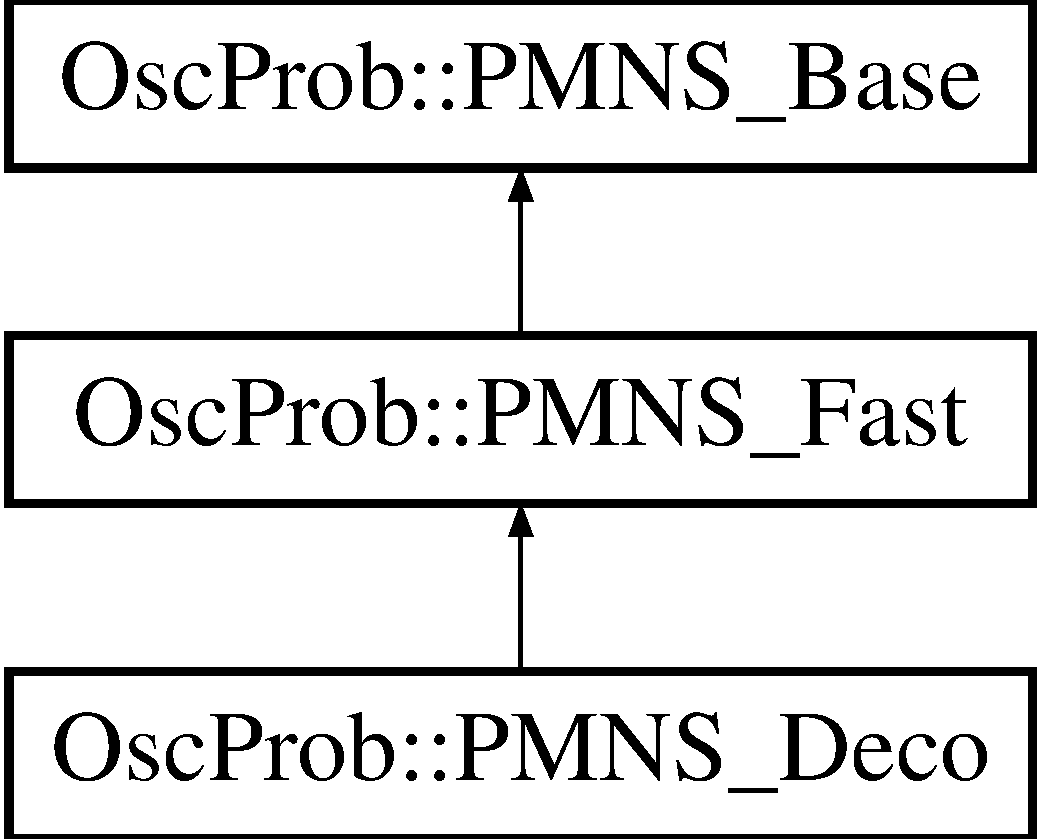
\includegraphics[height=3.000000cm]{classOscProb_1_1PMNS__Deco}
\end{center}
\end{figure}
\subsection*{Public Types}
\begin{DoxyCompactItemize}
\item 
typedef std\+::vector$<$ \hyperlink{EigenPoint_8h_a67ca8e107e20610c3fff78d5e726ece0}{complexD} $>$ \hyperlink{classOscProb_1_1PMNS__Deco_a430859c3da89582de577f8f7e75f2d16}{row}
\item 
typedef std\+::vector$<$ \hyperlink{classOscProb_1_1PMNS__Deco_a430859c3da89582de577f8f7e75f2d16}{row} $>$ \hyperlink{classOscProb_1_1PMNS__Deco_a77b4e0c041b6268910a270be0f5387c9}{matrix}
\end{DoxyCompactItemize}
\subsection*{Public Member Functions}
\begin{DoxyCompactItemize}
\item 
\hyperlink{classOscProb_1_1PMNS__Deco_a976dc43bb65547af5f4a27f5a8fccbba}{P\+M\+N\+S\+\_\+\+Deco} ()
\begin{DoxyCompactList}\small\item\em Constructor. \end{DoxyCompactList}\item 
virtual \hyperlink{classOscProb_1_1PMNS__Deco_a5539610ab44c510c204ae884fb8e2a0e}{$\sim$\+P\+M\+N\+S\+\_\+\+Deco} ()
\begin{DoxyCompactList}\small\item\em Destructor. \end{DoxyCompactList}\item 
virtual void \hyperlink{classOscProb_1_1PMNS__Deco_ac06a9c503d1c5b4a43c4eb797881898d}{Set\+Gamma} (int j, double val)
\begin{DoxyCompactList}\small\item\em Set any given decoherence parameter. \end{DoxyCompactList}\item 
virtual void \hyperlink{classOscProb_1_1PMNS__Deco_a1bc2d1fb1bab9841baa37eecc0135fe9}{Set\+Gamma32} (double val)
\begin{DoxyCompactList}\small\item\em Set the $\Gamma_{32}$ parameter. \end{DoxyCompactList}\item 
virtual void \hyperlink{classOscProb_1_1PMNS__Deco_a35e79054682aa88c55f4350c29336014}{Set\+Deco\+Angle} (double th)
\begin{DoxyCompactList}\small\item\em Set the decoherence angle. \end{DoxyCompactList}\item 
virtual void \hyperlink{classOscProb_1_1PMNS__Deco_afe7b8b9ae438d8b207bf75c2cfbb9fb8}{Set\+Power} (double n)
\begin{DoxyCompactList}\small\item\em Set the power index. \end{DoxyCompactList}\item 
virtual double \hyperlink{classOscProb_1_1PMNS__Deco_a73461e806063588a8e3a9d5d0dd201cb}{Get\+Gamma} (int i, int j)
\begin{DoxyCompactList}\small\item\em Get any given decoherence parameter. \end{DoxyCompactList}\item 
virtual double \hyperlink{classOscProb_1_1PMNS__Deco_a5dadf6a39dec4a229babeff6a650179c}{Get\+Deco\+Angle} ()
\begin{DoxyCompactList}\small\item\em Get the decoherence angle. \end{DoxyCompactList}\item 
virtual double \hyperlink{classOscProb_1_1PMNS__Deco_aa40b92e0f204f499a24b18ba399b8b0e}{Get\+Power} ()
\begin{DoxyCompactList}\small\item\em Get the power index. \end{DoxyCompactList}\item 
virtual void \hyperlink{classOscProb_1_1PMNS__Fast_ad849b2231d99c5d66fb3ade8efb896e1}{Set\+Mix} (double th12, double th23, double th13, double deltacp)
\begin{DoxyCompactList}\small\item\em Set the all mixing parameters at once. \end{DoxyCompactList}\item 
virtual void \hyperlink{classOscProb_1_1PMNS__Fast_a63733b246e6d2e609ce3de7a65ba5b9f}{Set\+Delta\+Msqrs} (double dm21, double dm32)
\begin{DoxyCompactList}\small\item\em Set both mass-\/splittings at once. \end{DoxyCompactList}\item 
virtual double \hyperlink{classOscProb_1_1PMNS__Base_aa2e10704d2d205a1ec8988de14b1a66f}{Prob} (std\+::vector$<$ \hyperlink{EigenPoint_8h_a67ca8e107e20610c3fff78d5e726ece0}{complexD} $>$ nu\+\_\+in, int flvf)
\begin{DoxyCompactList}\small\item\em Compute the probability of nu\+\_\+in going to flvf. \end{DoxyCompactList}\item 
virtual double \hyperlink{classOscProb_1_1PMNS__Base_a0190a79284289aacf682c78d7cef9a81}{Prob} (std\+::vector$<$ \hyperlink{EigenPoint_8h_a67ca8e107e20610c3fff78d5e726ece0}{complexD} $>$ nu\+\_\+in, int flvf, double E)
\begin{DoxyCompactList}\small\item\em Compute the probability of nu\+\_\+in going to flvf for energy E. \end{DoxyCompactList}\item 
virtual double \hyperlink{classOscProb_1_1PMNS__Base_a01fba31729345376705e02408e835f67}{Prob} (std\+::vector$<$ \hyperlink{EigenPoint_8h_a67ca8e107e20610c3fff78d5e726ece0}{complexD} $>$ nu\+\_\+in, int flvf, double E, double L)
\begin{DoxyCompactList}\small\item\em Compute the probability of nu\+\_\+in going to flvf for energy E and distance L. \end{DoxyCompactList}\item 
virtual double \hyperlink{classOscProb_1_1PMNS__Base_aec5c399b93261f1962a4b7dbbb44b973}{Prob} (int flvi, int flvf)
\begin{DoxyCompactList}\small\item\em Compute the probability of flvi going to flvf. \end{DoxyCompactList}\item 
virtual double \hyperlink{classOscProb_1_1PMNS__Base_aa3cee10639d5c0879ccb9e78d62128d3}{Prob} (int flvi, int flvf, double E)
\begin{DoxyCompactList}\small\item\em Compute the probability of flvi going to flvf for energy E. \end{DoxyCompactList}\item 
virtual double \hyperlink{classOscProb_1_1PMNS__Base_a6e0a74508d9d6db7be02e242b8467563}{Prob} (int flvi, int flvf, double E, double L)
\begin{DoxyCompactList}\small\item\em Compute the probability of flvi going to flvf for energy E and distance L. \end{DoxyCompactList}\item 
virtual double \hyperlink{classOscProb_1_1PMNS__Base_a89e54c80ae8a31effbab7b2b970606bb}{Avg\+Prob} (std\+::vector$<$ \hyperlink{EigenPoint_8h_a67ca8e107e20610c3fff78d5e726ece0}{complexD} $>$ nu\+\_\+in, int flvf, double E, double dE=0)
\begin{DoxyCompactList}\small\item\em Compute the average probability over a bin of energy. \end{DoxyCompactList}\item 
virtual double \hyperlink{classOscProb_1_1PMNS__Base_ac03f754160422e6600da8dbae0f803ed}{Avg\+Prob} (int flvi, int flvf, double E, double dE=0)
\begin{DoxyCompactList}\small\item\em Compute the average probability over a bin of energy. \end{DoxyCompactList}\item 
virtual double \hyperlink{classOscProb_1_1PMNS__Base_a19f160c045a01e5083506e925fb37d44}{Avg\+Prob\+LoE} (std\+::vector$<$ \hyperlink{EigenPoint_8h_a67ca8e107e20610c3fff78d5e726ece0}{complexD} $>$ nu\+\_\+in, int flvf, double LoE, double d\+LoE=0)
\begin{DoxyCompactList}\small\item\em Compute the average probability over a bin of L/E. \end{DoxyCompactList}\item 
virtual double \hyperlink{classOscProb_1_1PMNS__Base_ac19a92f4ef428a7333ca8eed76fca637}{Avg\+Prob\+LoE} (int flvi, int flvf, double LoE, double d\+LoE=0)
\begin{DoxyCompactList}\small\item\em Compute the average probability over a bin of L/E. \end{DoxyCompactList}\item 
virtual std\+::vector$<$ \hyperlink{EigenPoint_8h_a67ca8e107e20610c3fff78d5e726ece0}{complexD} $>$ \hyperlink{classOscProb_1_1PMNS__Base_a5092561dd8579d390c649eb60803ea98}{Get\+Mass\+Eigenstate} (int mi)
\begin{DoxyCompactList}\small\item\em Get a neutrino mass eigenstate. \end{DoxyCompactList}\item 
virtual void \hyperlink{classOscProb_1_1PMNS__Base_ace7875cf6d3bec161a2b7ed2690aec34}{Set\+Angle} (int i, int j, double th)
\begin{DoxyCompactList}\small\item\em Set the mixing angle theta\+\_\+ij. \end{DoxyCompactList}\item 
virtual void \hyperlink{classOscProb_1_1PMNS__Base_a4bef78cfcfc4e70b4ce79cdb8862c0a3}{Set\+Delta} (int i, int j, double delta)
\begin{DoxyCompactList}\small\item\em Set the CP phase delta\+\_\+ij. \end{DoxyCompactList}\item 
virtual void \hyperlink{classOscProb_1_1PMNS__Base_a492243b22fb1b783cd2943f507cff970}{Set\+Dm} (int j, double dm)
\begin{DoxyCompactList}\small\item\em Set the mass-\/splitting dm\+\_\+j1 in e\+V$^\wedge$2. \end{DoxyCompactList}\item 
virtual double \hyperlink{classOscProb_1_1PMNS__Base_acee137091304c919642293ddf015bbc8}{Get\+Angle} (int i, int j)
\begin{DoxyCompactList}\small\item\em Get the mixing angle theta\+\_\+ij. \end{DoxyCompactList}\item 
virtual double \hyperlink{classOscProb_1_1PMNS__Base_adb8dbc91d4286d2e7c8f768c59476241}{Get\+Delta} (int i, int j)
\begin{DoxyCompactList}\small\item\em Get the CP phase delta\+\_\+ij. \end{DoxyCompactList}\item 
virtual double \hyperlink{classOscProb_1_1PMNS__Base_ad26815ac5f4805d1259817e4936e5f8f}{Get\+Dm} (int j)
\begin{DoxyCompactList}\small\item\em Get the mass-\/splitting dm\+\_\+j1 in e\+V$^\wedge$2. \end{DoxyCompactList}\item 
virtual double \hyperlink{classOscProb_1_1PMNS__Base_a4ea861a6707ce1be3a54aad2b60f8632}{Get\+Dm\+Eff} (int j)
\begin{DoxyCompactList}\small\item\em Get the effective mass-\/splitting dm\+\_\+j1 in e\+V$^\wedge$2. \end{DoxyCompactList}\item 
virtual void \hyperlink{classOscProb_1_1PMNS__Base_a4de96ac9b6d1e9b029ab877e57d211ad}{Set\+Std\+Pars} ()
\begin{DoxyCompactList}\small\item\em Set P\+DG 3-\/flavor parameters. \end{DoxyCompactList}\item 
virtual void \hyperlink{classOscProb_1_1PMNS__Base_a95b3b0d0cab5e6a54b5ef99587f837c0}{Set\+Energy} (double E)
\begin{DoxyCompactList}\small\item\em Set the neutrino energy in GeV. \end{DoxyCompactList}\item 
virtual void \hyperlink{classOscProb_1_1PMNS__Base_a717e0348cf762f3961854e332a9b52e0}{Set\+Is\+Nu\+Bar} (bool is\+Nu\+Bar)
\begin{DoxyCompactList}\small\item\em Set the anti-\/neutrino flag. \end{DoxyCompactList}\item 
virtual double \hyperlink{classOscProb_1_1PMNS__Base_acc0d46cc4b8f911b40b807225003bbed}{Get\+Energy} ()
\begin{DoxyCompactList}\small\item\em Get the neutrino energy in GeV. \end{DoxyCompactList}\item 
virtual bool \hyperlink{classOscProb_1_1PMNS__Base_a2f7f2a028dfe7a90fff6b4f757972c2c}{Get\+Is\+Nu\+Bar} ()
\begin{DoxyCompactList}\small\item\em Get the anti-\/neutrino flag. \end{DoxyCompactList}\item 
virtual void \hyperlink{classOscProb_1_1PMNS__Base_ac3b644fd0a56347d304ceca4ae9d8875}{Set\+Path} (\hyperlink{structOscProb_1_1NuPath}{Osc\+Prob\+::\+Nu\+Path} p)
\begin{DoxyCompactList}\small\item\em Set a single path. \end{DoxyCompactList}\item 
virtual void \hyperlink{classOscProb_1_1PMNS__Base_a35b983270613072a3df58b574d80dbfd}{Set\+Path} (double length, double density, double zoa=0.\+5, int layer=0)
\begin{DoxyCompactList}\small\item\em Set a single path. \end{DoxyCompactList}\item 
virtual void \hyperlink{classOscProb_1_1PMNS__Base_a637d19dd850b4246507796526622643c}{Set\+Path} (std\+::vector$<$ \hyperlink{structOscProb_1_1NuPath}{Osc\+Prob\+::\+Nu\+Path} $>$ paths)
\begin{DoxyCompactList}\small\item\em Set a path sequence. \end{DoxyCompactList}\item 
virtual void \hyperlink{classOscProb_1_1PMNS__Base_a887dc9d4dc569ec0cdef3933b4c60efc}{Add\+Path} (\hyperlink{structOscProb_1_1NuPath}{Osc\+Prob\+::\+Nu\+Path} p)
\begin{DoxyCompactList}\small\item\em Add a path to the sequence. \end{DoxyCompactList}\item 
virtual void \hyperlink{classOscProb_1_1PMNS__Base_ab7f89ad9e7e1224adaa59d3c41594cd9}{Add\+Path} (double length, double density, double zoa=0.\+5, int layer=0)
\begin{DoxyCompactList}\small\item\em Add a path to the sequence. \end{DoxyCompactList}\item 
virtual void \hyperlink{classOscProb_1_1PMNS__Base_aefe521239031c418cfaaaa550a6e13bb}{Clear\+Path} ()
\begin{DoxyCompactList}\small\item\em Clear the path vector. \end{DoxyCompactList}\item 
virtual void \hyperlink{classOscProb_1_1PMNS__Base_a6241325b1bd28cafa556daaecbe4ed62}{Set\+Length} (double L)
\begin{DoxyCompactList}\small\item\em Set a single path lentgh in km. \end{DoxyCompactList}\item 
virtual void \hyperlink{classOscProb_1_1PMNS__Base_aa34a40a3b5abda0f252982d9ead3b520}{Set\+Length} (std\+::vector$<$ double $>$ L)
\begin{DoxyCompactList}\small\item\em Set multiple path lengths. \end{DoxyCompactList}\item 
virtual void \hyperlink{classOscProb_1_1PMNS__Base_ac74206f349687da141392c81e2ba6b0d}{Set\+Density} (double rho)
\begin{DoxyCompactList}\small\item\em Set single path density in g/cm$^\wedge$3. \end{DoxyCompactList}\item 
virtual void \hyperlink{classOscProb_1_1PMNS__Base_a858221d5510fe732dc6a101fd305cda0}{Set\+Density} (std\+::vector$<$ double $>$ rho)
\begin{DoxyCompactList}\small\item\em Set multiple path densities. \end{DoxyCompactList}\item 
virtual void \hyperlink{classOscProb_1_1PMNS__Base_a1bf3ea8fd2507fd2fd82d7410ff8f578}{Set\+ZoA} (double zoa)
\begin{DoxyCompactList}\small\item\em Set Z/A value for single path. \end{DoxyCompactList}\item 
virtual void \hyperlink{classOscProb_1_1PMNS__Base_a8495f8a320e1a21965e6a64aec92ad2a}{Set\+ZoA} (std\+::vector$<$ double $>$ zoa)
\begin{DoxyCompactList}\small\item\em Set multiple path Z/A values. \end{DoxyCompactList}\item 
virtual void \hyperlink{classOscProb_1_1PMNS__Base_a904e580edf89fb98bf9a6397739b4ebe}{Set\+Layers} (std\+::vector$<$ int $>$ lay)
\begin{DoxyCompactList}\small\item\em Set multiple path layer indices. \end{DoxyCompactList}\item 
virtual void \hyperlink{classOscProb_1_1PMNS__Base_add6533a9fc9acdfc7ae258b62570d78d}{Set\+Std\+Path} ()
\begin{DoxyCompactList}\small\item\em Set standard neutrino path. \end{DoxyCompactList}\item 
virtual std\+::vector$<$ \hyperlink{structOscProb_1_1NuPath}{Osc\+Prob\+::\+Nu\+Path} $>$ \hyperlink{classOscProb_1_1PMNS__Base_ac8e196f2e85a2b1caaf705073ee95a5c}{Get\+Path} ()
\begin{DoxyCompactList}\small\item\em Get the neutrino path sequence. \end{DoxyCompactList}\item 
virtual std\+::vector$<$ double $>$ \hyperlink{classOscProb_1_1PMNS__Base_a9eac8d768c1424755ee41f7e783af179}{Get\+Sample\+Points} (double LoE, double d\+LoE)
\begin{DoxyCompactList}\small\item\em Compute the sample points for a bin of L/E with width d\+LoE. \end{DoxyCompactList}\item 
virtual void \hyperlink{classOscProb_1_1PMNS__Base_aa94c1e1fff0ba731c75f7e633b023a9f}{Set\+Use\+Cache} (bool u=true)
\begin{DoxyCompactList}\small\item\em Set caching on/off. \end{DoxyCompactList}\item 
virtual void \hyperlink{classOscProb_1_1PMNS__Base_ac47fd33e69aa6490f99e2fd147a92f03}{Clear\+Cache} ()
\begin{DoxyCompactList}\small\item\em Clear the cache. \end{DoxyCompactList}\item 
virtual void \hyperlink{classOscProb_1_1PMNS__Base_ae67862cf58b0802487a14b047b012a78}{Set\+Max\+Cache} (int mc=1e6)
\begin{DoxyCompactList}\small\item\em Set max cache size. \end{DoxyCompactList}\end{DoxyCompactItemize}
\subsection*{Protected Member Functions}
\begin{DoxyCompactItemize}
\item 
virtual void \hyperlink{classOscProb_1_1PMNS__Deco_a393940f176614e3ffebeea40cfe78a62}{Reset\+To\+Flavour} (int flv)
\begin{DoxyCompactList}\small\item\em Reset neutrino state to pure flavour flv. \end{DoxyCompactList}\item 
virtual void \hyperlink{classOscProb_1_1PMNS__Deco_aa75341a3608bb12d7792a14e67ef2d5e}{Propagate\+Path} (\hyperlink{structOscProb_1_1NuPath}{Osc\+Prob\+::\+Nu\+Path} p)
\begin{DoxyCompactList}\small\item\em Propagate neutrino through a single path. \end{DoxyCompactList}\item 
virtual double \hyperlink{classOscProb_1_1PMNS__Deco_aa81f47ea36207b90a5feb9849060032d}{P} (int flv)
\begin{DoxyCompactList}\small\item\em Return the probability of final state in flavour flv. \end{DoxyCompactList}\item 
virtual \hyperlink{classOscProb_1_1PMNS__Deco_a77b4e0c041b6268910a270be0f5387c9}{matrix} \hyperlink{classOscProb_1_1PMNS__Deco_a8d6b547de294c0d52d4208bde44fe171}{Dot} (\hyperlink{classOscProb_1_1PMNS__Deco_a77b4e0c041b6268910a270be0f5387c9}{matrix} A, \hyperlink{classOscProb_1_1PMNS__Deco_a77b4e0c041b6268910a270be0f5387c9}{matrix} B)
\item 
virtual \hyperlink{classOscProb_1_1PMNS__Deco_a77b4e0c041b6268910a270be0f5387c9}{matrix} \hyperlink{classOscProb_1_1PMNS__Deco_aacc9909556ca22aca30620893e12b0db}{Mult} (\hyperlink{classOscProb_1_1PMNS__Deco_a77b4e0c041b6268910a270be0f5387c9}{matrix} A, \hyperlink{classOscProb_1_1PMNS__Deco_a77b4e0c041b6268910a270be0f5387c9}{matrix} B)
\item 
virtual \hyperlink{classOscProb_1_1PMNS__Deco_a77b4e0c041b6268910a270be0f5387c9}{matrix} \hyperlink{classOscProb_1_1PMNS__Deco_aca391ff02be7abc2fd3dba40e9ce2665}{C\+Transp} (\hyperlink{classOscProb_1_1PMNS__Deco_a77b4e0c041b6268910a270be0f5387c9}{matrix} A)
\item 
virtual void \hyperlink{classOscProb_1_1PMNS__Fast_a16248082308f9d2c332ebf1be0aa90c3}{Update\+Ham} ()
\begin{DoxyCompactList}\small\item\em Build the full Hamiltonian. \end{DoxyCompactList}\item 
virtual void \hyperlink{classOscProb_1_1PMNS__Fast_a8a0828401591e88c60e0051fbfe02d5e}{Solve\+Ham} ()
\begin{DoxyCompactList}\small\item\em Solve the full Hamiltonian for eigenvectors and eigenvalues. \end{DoxyCompactList}\item 
virtual void \hyperlink{classOscProb_1_1PMNS__Fast_a76dd5a761df8689c502b28ad0391f9e2}{Set\+Vacuum\+Eigensystem} ()
\begin{DoxyCompactList}\small\item\em Set the eigensystem to the analytic solution of the vacuum Hamiltonian. \end{DoxyCompactList}\item 
virtual void \hyperlink{classOscProb_1_1PMNS__Base_adf23b569112f9f9e0e592f01d79a5f3d}{Initialize\+Vectors} ()
\begin{DoxyCompactList}\small\item\em Initialize all member vectors with zeros. \end{DoxyCompactList}\item 
virtual bool \hyperlink{classOscProb_1_1PMNS__Base_abe533da5f64bec1f4724ab7b58606b77}{Try\+Cache} ()
\begin{DoxyCompactList}\small\item\em Try to find a cached eigensystem. \end{DoxyCompactList}\item 
virtual void \hyperlink{classOscProb_1_1PMNS__Base_a785c37fcea974628623c8881bb0fbbf9}{Fill\+Cache} ()
\begin{DoxyCompactList}\small\item\em Cache the current eigensystem. \end{DoxyCompactList}\item 
virtual void \hyperlink{classOscProb_1_1PMNS__Base_a986e6ebef09a7e2eb7fee16a4c2c834d}{Set\+Cur\+Path} (\hyperlink{structOscProb_1_1NuPath}{Osc\+Prob\+::\+Nu\+Path} p)
\begin{DoxyCompactList}\small\item\em Set the path currently in use by the class. \end{DoxyCompactList}\item 
virtual void \hyperlink{classOscProb_1_1PMNS__Base_aba565962a440d14bee7a2a96d2eca2c5}{Set\+Att} (double att, int idx)
\begin{DoxyCompactList}\small\item\em Set one of the path attributes. \end{DoxyCompactList}\item 
virtual void \hyperlink{classOscProb_1_1PMNS__Base_aa001479b5f5828c3d16ed087f96ecbcc}{Set\+Att} (std\+::vector$<$ double $>$ att, int idx)
\begin{DoxyCompactList}\small\item\em Set all values of a path attribute. \end{DoxyCompactList}\item 
virtual void \hyperlink{classOscProb_1_1PMNS__Base_a6a3cf45bbe2349abf06708b65677c044}{RotateH} (int i, int j, std\+::vector$<$ std\+::vector$<$ \hyperlink{EigenPoint_8h_a67ca8e107e20610c3fff78d5e726ece0}{complexD} $>$ $>$ \&Ham)
\begin{DoxyCompactList}\small\item\em Rotate the Hamiltonian by theta\+\_\+ij and delta\+\_\+ij. \end{DoxyCompactList}\item 
virtual void \hyperlink{classOscProb_1_1PMNS__Base_ae52554477ad3250daa5adb8c32cab0b4}{Rotate\+State} (int i, int j)
\begin{DoxyCompactList}\small\item\em Rotate the neutrino state by theta\+\_\+ij and delta\+\_\+ij. \end{DoxyCompactList}\item 
virtual void \hyperlink{classOscProb_1_1PMNS__Base_ad0faf5eae755afb1baa1fcd5ffebad41}{Build\+Hms} ()
\begin{DoxyCompactList}\small\item\em Build the matrix of masses squared. \end{DoxyCompactList}\item 
virtual void \hyperlink{classOscProb_1_1PMNS__Base_a054e3a8b05b9a958b6fa416e4a835e3e}{Propagate} ()
\begin{DoxyCompactList}\small\item\em Propagate neutrino through full path. \end{DoxyCompactList}\end{DoxyCompactItemize}
\subsection*{Protected Attributes}
\begin{DoxyCompactItemize}
\item 
double \hyperlink{classOscProb_1_1PMNS__Deco_ae2f30ac9f8b25344959f1698616d337a}{f\+Gamma} \mbox{[}3\mbox{]}
\begin{DoxyCompactList}\small\item\em Stores each decoherence parameter. \end{DoxyCompactList}\item 
double \hyperlink{classOscProb_1_1PMNS__Deco_a19fdcdf9a8b2bd9677f72ca1fd77dc3e}{f\+Power}
\begin{DoxyCompactList}\small\item\em Stores the power index parameter. \end{DoxyCompactList}\item 
\hyperlink{classOscProb_1_1PMNS__Deco_a77b4e0c041b6268910a270be0f5387c9}{matrix} \hyperlink{classOscProb_1_1PMNS__Deco_a0488d62b4ef4cf5b43425769f5fcdbdf}{f\+Rho}
\begin{DoxyCompactList}\small\item\em The neutrino density matrix state. \end{DoxyCompactList}\item 
\hyperlink{EigenPoint_8h_a67ca8e107e20610c3fff78d5e726ece0}{complexD} \hyperlink{classOscProb_1_1PMNS__Fast_a94286a881bc53dd512a89d548346b611}{f\+Ham} \mbox{[}3\mbox{]}\mbox{[}3\mbox{]}
\begin{DoxyCompactList}\small\item\em The full hamiltonian. \end{DoxyCompactList}\item 
int \hyperlink{classOscProb_1_1PMNS__Base_a24bb74bed63569dfe88b18fa6a08060e}{f\+Num\+Nus}
\begin{DoxyCompactList}\small\item\em Number of neutrino flavours. \end{DoxyCompactList}\item 
std\+::vector$<$ double $>$ \hyperlink{classOscProb_1_1PMNS__Base_a406a31c3b5d620e5a0cace5b411f9f70}{f\+Dm}
\begin{DoxyCompactList}\small\item\em m$^\wedge$2\+\_\+i -\/ m$^\wedge$2\+\_\+1 in vacuum \end{DoxyCompactList}\item 
std\+::vector$<$ std\+::vector$<$ double $>$ $>$ \hyperlink{classOscProb_1_1PMNS__Base_a1976887cd658dd86b2336c181f1470b4}{f\+Theta}
\begin{DoxyCompactList}\small\item\em theta\mbox{[}i\mbox{]}\mbox{[}j\mbox{]} mixing angle \end{DoxyCompactList}\item 
std\+::vector$<$ std\+::vector$<$ double $>$ $>$ \hyperlink{classOscProb_1_1PMNS__Base_ab2a5fa40e689b221c8a7d2c17213810d}{f\+Delta}
\begin{DoxyCompactList}\small\item\em delta\mbox{[}i\mbox{]}\mbox{[}j\mbox{]} CP violating phase \end{DoxyCompactList}\item 
std\+::vector$<$ \hyperlink{EigenPoint_8h_a67ca8e107e20610c3fff78d5e726ece0}{complexD} $>$ \hyperlink{classOscProb_1_1PMNS__Base_abf99f2339e3ee989600740b5d88063e8}{f\+Nu\+State}
\begin{DoxyCompactList}\small\item\em The neutrino current state. \end{DoxyCompactList}\item 
std\+::vector$<$ std\+::vector$<$ \hyperlink{EigenPoint_8h_a67ca8e107e20610c3fff78d5e726ece0}{complexD} $>$ $>$ \hyperlink{classOscProb_1_1PMNS__Base_acd3c8783e7603081eab316ea4c86c766}{f\+Hms}
\begin{DoxyCompactList}\small\item\em matrix H$\ast$2E in e\+V$^\wedge$2 \end{DoxyCompactList}\item 
std\+::vector$<$ \hyperlink{EigenPoint_8h_a67ca8e107e20610c3fff78d5e726ece0}{complexD} $>$ \hyperlink{classOscProb_1_1PMNS__Base_ab8d26b722047d49d977f5f2d83026ede}{f\+Phases}
\begin{DoxyCompactList}\small\item\em Buffer for oscillation phases. \end{DoxyCompactList}\item 
std\+::vector$<$ \hyperlink{EigenPoint_8h_a67ca8e107e20610c3fff78d5e726ece0}{complexD} $>$ \hyperlink{classOscProb_1_1PMNS__Base_a5440bc3efa466a37649601abce559e3e}{f\+Buffer}
\begin{DoxyCompactList}\small\item\em Buffer for neutrino state tranformations. \end{DoxyCompactList}\item 
std\+::vector$<$ double $>$ \hyperlink{classOscProb_1_1PMNS__Base_a6319c34d7decbb9d7d6da279c06e8c2d}{f\+Eval}
\begin{DoxyCompactList}\small\item\em Eigenvalues of the Hamiltonian. \end{DoxyCompactList}\item 
std\+::vector$<$ std\+::vector$<$ \hyperlink{EigenPoint_8h_a67ca8e107e20610c3fff78d5e726ece0}{complexD} $>$ $>$ \hyperlink{classOscProb_1_1PMNS__Base_a87be137356c5f27ab83cab5e1298ef8f}{f\+Evec}
\begin{DoxyCompactList}\small\item\em Eigenvectors of the Hamiltonian. \end{DoxyCompactList}\item 
double \hyperlink{classOscProb_1_1PMNS__Base_a2800af6d436972f3e900867790c046b0}{f\+Energy}
\begin{DoxyCompactList}\small\item\em Neutrino energy. \end{DoxyCompactList}\item 
bool \hyperlink{classOscProb_1_1PMNS__Base_a0ebaeaefab36a3ff381c6293faedfdd6}{f\+Is\+Nu\+Bar}
\begin{DoxyCompactList}\small\item\em Anti-\/neutrino flag. \end{DoxyCompactList}\item 
std\+::vector$<$ \hyperlink{structOscProb_1_1NuPath}{Osc\+Prob\+::\+Nu\+Path} $>$ \hyperlink{classOscProb_1_1PMNS__Base_a69db9d57e12fc7cbe0431bc6c18fac93}{f\+Nu\+Paths}
\begin{DoxyCompactList}\small\item\em Vector of neutrino paths. \end{DoxyCompactList}\item 
\hyperlink{structOscProb_1_1NuPath}{Osc\+Prob\+::\+Nu\+Path} \hyperlink{classOscProb_1_1PMNS__Base_a849437aa8891fe042e86886ce8f81c6e}{f\+Path}
\begin{DoxyCompactList}\small\item\em Current neutrino path. \end{DoxyCompactList}\item 
bool \hyperlink{classOscProb_1_1PMNS__Base_a9ac3cadeac8db1b90f3152f476244780}{f\+Built\+Hms}
\begin{DoxyCompactList}\small\item\em Tag to avoid rebuilding Hms. \end{DoxyCompactList}\item 
bool \hyperlink{classOscProb_1_1PMNS__Base_a6dc5cd010d2d70b2324745b4e53e9839}{f\+Got\+ES}
\begin{DoxyCompactList}\small\item\em Tag to avoid recalculating eigensystem. \end{DoxyCompactList}\item 
bool \hyperlink{classOscProb_1_1PMNS__Base_ad28c12ef897b5555eda509ea55c99107}{f\+Use\+Cache}
\begin{DoxyCompactList}\small\item\em Flag for whether to use caching. \end{DoxyCompactList}\item 
double \hyperlink{classOscProb_1_1PMNS__Base_a0b4c41a27de281472453a1912cbc1e64}{f\+Cache\+Prec}
\begin{DoxyCompactList}\small\item\em Precision of cache matching. \end{DoxyCompactList}\item 
int \hyperlink{classOscProb_1_1PMNS__Base_a74c13356eafec2490d8c3c19759ba7f0}{f\+Max\+Cache}
\begin{DoxyCompactList}\small\item\em Maximum cache size. \end{DoxyCompactList}\item 
std\+::set$<$ \hyperlink{structOscProb_1_1EigenPoint}{Osc\+Prob\+::\+Eigen\+Point} $>$ \hyperlink{classOscProb_1_1PMNS__Base_a8159424f20197a3a7145fe3bf2c11176}{f\+Mix\+Cache}
\begin{DoxyCompactList}\small\item\em Caching set of eigensystems. \end{DoxyCompactList}\item 
\hyperlink{structOscProb_1_1EigenPoint}{Eigen\+Point} \hyperlink{classOscProb_1_1PMNS__Base_ab1fe4800ee3ae48df4fc942dce00e0d3}{f\+Probe}
\begin{DoxyCompactList}\small\item\em Eigenp\+Point to try. \end{DoxyCompactList}\end{DoxyCompactItemize}
\subsection*{Static Protected Attributes}
\begin{DoxyCompactItemize}
\item 
static const \hyperlink{EigenPoint_8h_a67ca8e107e20610c3fff78d5e726ece0}{complexD} \hyperlink{classOscProb_1_1PMNS__Base_a05e595848c2521dc795efa7645728b94}{zero}
\begin{DoxyCompactList}\small\item\em zero in complex \end{DoxyCompactList}\item 
static const \hyperlink{EigenPoint_8h_a67ca8e107e20610c3fff78d5e726ece0}{complexD} \hyperlink{classOscProb_1_1PMNS__Base_a7d1d0bbcab30a1fd8c368c40134c51ff}{one}
\begin{DoxyCompactList}\small\item\em one in complex \end{DoxyCompactList}\item 
static const double \hyperlink{classOscProb_1_1PMNS__Base_a382ddd7b76ca89b43f22614a2ea7327b}{k\+Km2eV} = 1.\+0 / 1.\+973269788e-\/10
\begin{DoxyCompactList}\small\item\em km to e\+V$^\wedge$-\/1 \end{DoxyCompactList}\item 
static const double \hyperlink{classOscProb_1_1PMNS__Base_a326fc5016d7dd7ce05682c06cdcb6d94}{k\+K2} = 1e-\/3 $\ast$ k\+N\+A / pow(k\+Km2e\+V,3)
\begin{DoxyCompactList}\small\item\em mol/\+Ge\+V$^\wedge$2/cm$^\wedge$3 to eV \end{DoxyCompactList}\item 
static const double \hyperlink{classOscProb_1_1PMNS__Base_ad36a0a6bf58d6ec093d3947784bd89e9}{k\+Ge\+V2eV} = 1.\+0e+09
\begin{DoxyCompactList}\small\item\em GeV to eV. \end{DoxyCompactList}\item 
static const double \hyperlink{classOscProb_1_1PMNS__Base_a69355e770b89e99437c2b8a66e48eeb9}{k\+NA} = 6.\+022140857e23
\begin{DoxyCompactList}\small\item\em Avogadro constant. \end{DoxyCompactList}\item 
static const double \hyperlink{classOscProb_1_1PMNS__Base_a7f26a3456128234b2ae6cc9141a6532f}{k\+Gf} = 1.\+1663787e-\/05
\begin{DoxyCompactList}\small\item\em G\+\_\+F in units of Ge\+V$^\wedge$-\/2. \end{DoxyCompactList}\end{DoxyCompactItemize}


\subsection{Detailed Description}
This class expands the \hyperlink{classOscProb_1_1PMNS__Fast}{P\+M\+N\+S\+\_\+\+Fast} class including a effects from decoherence in an increasing entropy and energy conserving model.

The model assumes a power law energy dependence of the decoherence parameters and that decoherence occurs in the effective mass basis.

\begin{DoxySeeAlso}{See also}
\hyperlink{classOscProb_1_1PMNS__Fast}{P\+M\+N\+S\+\_\+\+Fast}
\end{DoxySeeAlso}
\begin{DoxyAuthor}{Author}
coelho@lal.\+in2p3.\+fr 
\end{DoxyAuthor}


Definition at line 24 of file P\+M\+N\+S\+\_\+\+Deco.\+h.



\subsection{Member Typedef Documentation}
\mbox{\Hypertarget{classOscProb_1_1PMNS__Deco_a77b4e0c041b6268910a270be0f5387c9}\label{classOscProb_1_1PMNS__Deco_a77b4e0c041b6268910a270be0f5387c9}} 
\index{Osc\+Prob\+::\+P\+M\+N\+S\+\_\+\+Deco@{Osc\+Prob\+::\+P\+M\+N\+S\+\_\+\+Deco}!matrix@{matrix}}
\index{matrix@{matrix}!Osc\+Prob\+::\+P\+M\+N\+S\+\_\+\+Deco@{Osc\+Prob\+::\+P\+M\+N\+S\+\_\+\+Deco}}
\subsubsection{\texorpdfstring{matrix}{matrix}}
{\footnotesize\ttfamily typedef std\+::vector$<$\hyperlink{classOscProb_1_1PMNS__Deco_a430859c3da89582de577f8f7e75f2d16}{row}$>$ \hyperlink{classOscProb_1_1PMNS__Deco_a77b4e0c041b6268910a270be0f5387c9}{Osc\+Prob\+::\+P\+M\+N\+S\+\_\+\+Deco\+::matrix}}



Definition at line 53 of file P\+M\+N\+S\+\_\+\+Deco.\+h.

\mbox{\Hypertarget{classOscProb_1_1PMNS__Deco_a430859c3da89582de577f8f7e75f2d16}\label{classOscProb_1_1PMNS__Deco_a430859c3da89582de577f8f7e75f2d16}} 
\index{Osc\+Prob\+::\+P\+M\+N\+S\+\_\+\+Deco@{Osc\+Prob\+::\+P\+M\+N\+S\+\_\+\+Deco}!row@{row}}
\index{row@{row}!Osc\+Prob\+::\+P\+M\+N\+S\+\_\+\+Deco@{Osc\+Prob\+::\+P\+M\+N\+S\+\_\+\+Deco}}
\subsubsection{\texorpdfstring{row}{row}}
{\footnotesize\ttfamily typedef std\+::vector$<$\hyperlink{EigenPoint_8h_a67ca8e107e20610c3fff78d5e726ece0}{complexD}$>$ \hyperlink{classOscProb_1_1PMNS__Deco_a430859c3da89582de577f8f7e75f2d16}{Osc\+Prob\+::\+P\+M\+N\+S\+\_\+\+Deco\+::row}}



Definition at line 52 of file P\+M\+N\+S\+\_\+\+Deco.\+h.



\subsection{Constructor \& Destructor Documentation}
\mbox{\Hypertarget{classOscProb_1_1PMNS__Deco_a976dc43bb65547af5f4a27f5a8fccbba}\label{classOscProb_1_1PMNS__Deco_a976dc43bb65547af5f4a27f5a8fccbba}} 
\index{Osc\+Prob\+::\+P\+M\+N\+S\+\_\+\+Deco@{Osc\+Prob\+::\+P\+M\+N\+S\+\_\+\+Deco}!P\+M\+N\+S\+\_\+\+Deco@{P\+M\+N\+S\+\_\+\+Deco}}
\index{P\+M\+N\+S\+\_\+\+Deco@{P\+M\+N\+S\+\_\+\+Deco}!Osc\+Prob\+::\+P\+M\+N\+S\+\_\+\+Deco@{Osc\+Prob\+::\+P\+M\+N\+S\+\_\+\+Deco}}
\subsubsection{\texorpdfstring{P\+M\+N\+S\+\_\+\+Deco()}{PMNS\_Deco()}}
{\footnotesize\ttfamily P\+M\+N\+S\+\_\+\+Deco\+::\+P\+M\+N\+S\+\_\+\+Deco (\begin{DoxyParamCaption}{ }\end{DoxyParamCaption})}

Constructor. \begin{DoxySeeAlso}{See also}
\hyperlink{classOscProb_1_1PMNS__Base_aa53e83b03a9cf4bdfa0a07136bd17a79}{P\+M\+N\+S\+\_\+\+Base\+::\+P\+M\+N\+S\+\_\+\+Base}
\end{DoxySeeAlso}
This class is restricted to 3 neutrino flavours. 

Definition at line 28 of file P\+M\+N\+S\+\_\+\+Deco.\+cxx.



References Set\+Deco\+Angle(), Set\+Gamma(), Set\+Power(), and Osc\+Prob\+::\+P\+M\+N\+S\+\_\+\+Base\+::\+Set\+Std\+Path().


\begin{DoxyCode}
28                      : \hyperlink{classOscProb_1_1PMNS__Fast_a2bbac744bf63753105d766a860af7c0d}{PMNS\_Fast}(), \hyperlink{classOscProb_1_1PMNS__Deco_ae2f30ac9f8b25344959f1698616d337a}{fGamma}(),
29 \hyperlink{classOscProb_1_1PMNS__Deco_a0488d62b4ef4cf5b43425769f5fcdbdf}{fRho}(3, \hyperlink{classOscProb_1_1PMNS__Deco_a430859c3da89582de577f8f7e75f2d16}{row}(3,0))
30 \{
31   \hyperlink{classOscProb_1_1PMNS__Base_add6533a9fc9acdfc7ae258b62570d78d}{SetStdPath}();
32   \hyperlink{classOscProb_1_1PMNS__Deco_ac06a9c503d1c5b4a43c4eb797881898d}{SetGamma}(2,0);
33   \hyperlink{classOscProb_1_1PMNS__Deco_ac06a9c503d1c5b4a43c4eb797881898d}{SetGamma}(3,0);
34   \hyperlink{classOscProb_1_1PMNS__Deco_a35e79054682aa88c55f4350c29336014}{SetDecoAngle}(0);
35   \hyperlink{classOscProb_1_1PMNS__Deco_afe7b8b9ae438d8b207bf75c2cfbb9fb8}{SetPower}(0);
36 \}
\end{DoxyCode}
\mbox{\Hypertarget{classOscProb_1_1PMNS__Deco_a5539610ab44c510c204ae884fb8e2a0e}\label{classOscProb_1_1PMNS__Deco_a5539610ab44c510c204ae884fb8e2a0e}} 
\index{Osc\+Prob\+::\+P\+M\+N\+S\+\_\+\+Deco@{Osc\+Prob\+::\+P\+M\+N\+S\+\_\+\+Deco}!````~P\+M\+N\+S\+\_\+\+Deco@{$\sim$\+P\+M\+N\+S\+\_\+\+Deco}}
\index{````~P\+M\+N\+S\+\_\+\+Deco@{$\sim$\+P\+M\+N\+S\+\_\+\+Deco}!Osc\+Prob\+::\+P\+M\+N\+S\+\_\+\+Deco@{Osc\+Prob\+::\+P\+M\+N\+S\+\_\+\+Deco}}
\subsubsection{\texorpdfstring{$\sim$\+P\+M\+N\+S\+\_\+\+Deco()}{~PMNS\_Deco()}}
{\footnotesize\ttfamily P\+M\+N\+S\+\_\+\+Deco\+::$\sim$\+P\+M\+N\+S\+\_\+\+Deco (\begin{DoxyParamCaption}{ }\end{DoxyParamCaption})\hspace{0.3cm}{\ttfamily [virtual]}}

Nothing to clean. 

Definition at line 42 of file P\+M\+N\+S\+\_\+\+Deco.\+cxx.


\begin{DoxyCode}
42 \{\}
\end{DoxyCode}


\subsection{Member Function Documentation}
\mbox{\Hypertarget{classOscProb_1_1PMNS__Base_a887dc9d4dc569ec0cdef3933b4c60efc}\label{classOscProb_1_1PMNS__Base_a887dc9d4dc569ec0cdef3933b4c60efc}} 
\index{Osc\+Prob\+::\+P\+M\+N\+S\+\_\+\+Deco@{Osc\+Prob\+::\+P\+M\+N\+S\+\_\+\+Deco}!Add\+Path@{Add\+Path}}
\index{Add\+Path@{Add\+Path}!Osc\+Prob\+::\+P\+M\+N\+S\+\_\+\+Deco@{Osc\+Prob\+::\+P\+M\+N\+S\+\_\+\+Deco}}
\subsubsection{\texorpdfstring{Add\+Path()}{AddPath()}\hspace{0.1cm}{\footnotesize\ttfamily [1/2]}}
{\footnotesize\ttfamily void P\+M\+N\+S\+\_\+\+Base\+::\+Add\+Path (\begin{DoxyParamCaption}\item[{\hyperlink{structOscProb_1_1NuPath}{Osc\+Prob\+::\+Nu\+Path}}]{p }\end{DoxyParamCaption})\hspace{0.3cm}{\ttfamily [virtual]}, {\ttfamily [inherited]}}

Add a path to the sequence. 
\begin{DoxyParams}{Parameters}
{\em p} & -\/ A neutrino path segment \\
\hline
\end{DoxyParams}


Definition at line 351 of file P\+M\+N\+S\+\_\+\+Base.\+cxx.



References Osc\+Prob\+::\+P\+M\+N\+S\+\_\+\+Base\+::f\+Nu\+Paths.



Referenced by Osc\+Prob\+::\+P\+M\+N\+S\+\_\+\+Base\+::\+Add\+Path(), Osc\+Prob\+::\+P\+M\+N\+S\+\_\+\+Base\+::\+Set\+Att(), and Osc\+Prob\+::\+P\+M\+N\+S\+\_\+\+Base\+::\+Set\+Path().


\begin{DoxyCode}
351                                \{
352 
353   \hyperlink{classOscProb_1_1PMNS__Base_a69db9d57e12fc7cbe0431bc6c18fac93}{fNuPaths}.push\_back(p);
354 
355 \}
\end{DoxyCode}
\mbox{\Hypertarget{classOscProb_1_1PMNS__Base_ab7f89ad9e7e1224adaa59d3c41594cd9}\label{classOscProb_1_1PMNS__Base_ab7f89ad9e7e1224adaa59d3c41594cd9}} 
\index{Osc\+Prob\+::\+P\+M\+N\+S\+\_\+\+Deco@{Osc\+Prob\+::\+P\+M\+N\+S\+\_\+\+Deco}!Add\+Path@{Add\+Path}}
\index{Add\+Path@{Add\+Path}!Osc\+Prob\+::\+P\+M\+N\+S\+\_\+\+Deco@{Osc\+Prob\+::\+P\+M\+N\+S\+\_\+\+Deco}}
\subsubsection{\texorpdfstring{Add\+Path()}{AddPath()}\hspace{0.1cm}{\footnotesize\ttfamily [2/2]}}
{\footnotesize\ttfamily void P\+M\+N\+S\+\_\+\+Base\+::\+Add\+Path (\begin{DoxyParamCaption}\item[{double}]{length,  }\item[{double}]{density,  }\item[{double}]{zoa = {\ttfamily 0.5},  }\item[{int}]{layer = {\ttfamily 0} }\end{DoxyParamCaption})\hspace{0.3cm}{\ttfamily [virtual]}, {\ttfamily [inherited]}}

Add a path to the sequence defining attributes directly. 
\begin{DoxyParams}{Parameters}
{\em length} & -\/ The length of the path segment in km \\
\hline
{\em density} & -\/ The density of the path segment in g/cm$^\wedge$3 \\
\hline
{\em zoa} & -\/ The effective Z/A of the path segment \\
\hline
{\em layer} & -\/ An index to identify the layer type (e.\+g. earth inner core) \\
\hline
\end{DoxyParams}


Definition at line 365 of file P\+M\+N\+S\+\_\+\+Base.\+cxx.



References Osc\+Prob\+::\+P\+M\+N\+S\+\_\+\+Base\+::\+Add\+Path().


\begin{DoxyCode}
365                                                                            \{
366 
367   \hyperlink{classOscProb_1_1PMNS__Base_a887dc9d4dc569ec0cdef3933b4c60efc}{AddPath}(\hyperlink{structOscProb_1_1NuPath}{NuPath}(length, density, zoa, layer));
368 
369 \}
\end{DoxyCode}
\mbox{\Hypertarget{classOscProb_1_1PMNS__Base_a89e54c80ae8a31effbab7b2b970606bb}\label{classOscProb_1_1PMNS__Base_a89e54c80ae8a31effbab7b2b970606bb}} 
\index{Osc\+Prob\+::\+P\+M\+N\+S\+\_\+\+Deco@{Osc\+Prob\+::\+P\+M\+N\+S\+\_\+\+Deco}!Avg\+Prob@{Avg\+Prob}}
\index{Avg\+Prob@{Avg\+Prob}!Osc\+Prob\+::\+P\+M\+N\+S\+\_\+\+Deco@{Osc\+Prob\+::\+P\+M\+N\+S\+\_\+\+Deco}}
\subsubsection{\texorpdfstring{Avg\+Prob()}{AvgProb()}\hspace{0.1cm}{\footnotesize\ttfamily [1/2]}}
{\footnotesize\ttfamily double P\+M\+N\+S\+\_\+\+Base\+::\+Avg\+Prob (\begin{DoxyParamCaption}\item[{std\+::vector$<$ \hyperlink{EigenPoint_8h_a67ca8e107e20610c3fff78d5e726ece0}{complexD} $>$}]{nu\+\_\+in,  }\item[{int}]{flvf,  }\item[{double}]{E,  }\item[{double}]{dE = {\ttfamily 0} }\end{DoxyParamCaption})\hspace{0.3cm}{\ttfamily [virtual]}, {\ttfamily [inherited]}}

Compute the average probability of nu\+\_\+in going to flvf over a bin of energy E with width dE.

This gets transformed into L/E, since the oscillation terms have arguments linear in L/E and not E.

This function works best for single paths. In multiple paths the accuracy may be somewhat worse. If needed, average over smaller energy ranges.

Flavours are\+: 
\begin{DoxyPre}
  0 = nue, 1 = numu, 2 = nutau
  3 = sterile\_1, 4 = sterile\_2, etc.
\end{DoxyPre}
 
\begin{DoxyParams}{Parameters}
{\em nu\+\_\+in} & -\/ The neutrino initial state in flavour. \\
\hline
{\em flvf} & -\/ The neutrino final flavour. \\
\hline
{\em E} & -\/ The neutrino energy in the bin center in GeV \\
\hline
{\em dE} & -\/ The energy bin width in GeV\\
\hline
\end{DoxyParams}
\begin{DoxyReturn}{Returns}
Average neutrino oscillation probability 
\end{DoxyReturn}


Definition at line 1386 of file P\+M\+N\+S\+\_\+\+Base.\+cxx.



References Osc\+Prob\+::\+Avg\+Path(), Osc\+Prob\+::\+P\+M\+N\+S\+\_\+\+Base\+::\+Avg\+Prob\+Lo\+E(), Osc\+Prob\+::\+P\+M\+N\+S\+\_\+\+Base\+::f\+Nu\+Paths, Osc\+Prob\+::\+P\+M\+N\+S\+\_\+\+Base\+::f\+Path, Osc\+Prob\+::\+Nu\+Path\+::length, Osc\+Prob\+::\+P\+M\+N\+S\+\_\+\+Base\+::\+Prob(), and Osc\+Prob\+::\+P\+M\+N\+S\+\_\+\+Base\+::\+Set\+Cur\+Path().



Referenced by Osc\+Prob\+::\+P\+M\+N\+S\+\_\+\+Base\+::\+Avg\+Prob().


\begin{DoxyCode}
1387 \{
1388 
1389   \textcolor{comment}{// Do nothing if energy is not positive}
1390   \textcolor{keywordflow}{if}(E<=0) \textcolor{keywordflow}{return} 0;
1391 
1392   \textcolor{keywordflow}{if}(\hyperlink{classOscProb_1_1PMNS__Base_a69db9d57e12fc7cbe0431bc6c18fac93}{fNuPaths}.empty()) \textcolor{keywordflow}{return} 0;
1393 
1394   \textcolor{comment}{// Don't average zero width}
1395   \textcolor{keywordflow}{if}(dE<=0) \textcolor{keywordflow}{return} \hyperlink{classOscProb_1_1PMNS__Base_aa2e10704d2d205a1ec8988de14b1a66f}{Prob}(nu\_in, flvf, E);
1396 
1397   \textcolor{comment}{// Make sure fPath is set}
1398   \textcolor{comment}{// Use average if multiple paths}
1399   \hyperlink{classOscProb_1_1PMNS__Base_a986e6ebef09a7e2eb7fee16a4c2c834d}{SetCurPath}(\hyperlink{namespaceOscProb_a999a7944bad8bc72d7ee9f56f81a210e}{AvgPath}(\hyperlink{classOscProb_1_1PMNS__Base_a69db9d57e12fc7cbe0431bc6c18fac93}{fNuPaths}));
1400 
1401   \textcolor{comment}{// Define L/E variables}
1402   \textcolor{keywordtype}{double} LoE = 0;
1403   \textcolor{keywordtype}{double} dLoE = 0;
1404 
1405   \textcolor{comment}{// Set a minimum energy}
1406   \textcolor{keywordtype}{double} minE = 0.1 * E;
1407 
1408   \textcolor{comment}{// Transform range to L/E}
1409   \textcolor{comment}{// Full range if low edge > minE}
1410   \textcolor{keywordflow}{if}(E-dE/2 > minE)\{
1411     LoE = 0.5 * (\hyperlink{classOscProb_1_1PMNS__Base_a849437aa8891fe042e86886ce8f81c6e}{fPath}.\hyperlink{structOscProb_1_1NuPath_af22660894b6e25cf835500381b155557}{length}/(E-dE/2) + \hyperlink{classOscProb_1_1PMNS__Base_a849437aa8891fe042e86886ce8f81c6e}{fPath}.\hyperlink{structOscProb_1_1NuPath_af22660894b6e25cf835500381b155557}{length}/(E+dE/2));
1412     dLoE = \hyperlink{classOscProb_1_1PMNS__Base_a849437aa8891fe042e86886ce8f81c6e}{fPath}.\hyperlink{structOscProb_1_1NuPath_af22660894b6e25cf835500381b155557}{length}/(E-dE/2) - \hyperlink{classOscProb_1_1PMNS__Base_a849437aa8891fe042e86886ce8f81c6e}{fPath}.\hyperlink{structOscProb_1_1NuPath_af22660894b6e25cf835500381b155557}{length}/(E+dE/2);
1413   \}
1414   \textcolor{comment}{// Else start at minE}
1415   \textcolor{keywordflow}{else}\{
1416     LoE = 0.5 * (\hyperlink{classOscProb_1_1PMNS__Base_a849437aa8891fe042e86886ce8f81c6e}{fPath}.\hyperlink{structOscProb_1_1NuPath_af22660894b6e25cf835500381b155557}{length}/minE + \hyperlink{classOscProb_1_1PMNS__Base_a849437aa8891fe042e86886ce8f81c6e}{fPath}.\hyperlink{structOscProb_1_1NuPath_af22660894b6e25cf835500381b155557}{length}/(E+dE/2));
1417     dLoE = \hyperlink{classOscProb_1_1PMNS__Base_a849437aa8891fe042e86886ce8f81c6e}{fPath}.\hyperlink{structOscProb_1_1NuPath_af22660894b6e25cf835500381b155557}{length}/minE - \hyperlink{classOscProb_1_1PMNS__Base_a849437aa8891fe042e86886ce8f81c6e}{fPath}.\hyperlink{structOscProb_1_1NuPath_af22660894b6e25cf835500381b155557}{length}/(E+dE/2);
1418   \}
1419 
1420   \textcolor{comment}{// Compute average in LoE}
1421   \textcolor{keywordflow}{return} \hyperlink{classOscProb_1_1PMNS__Base_a19f160c045a01e5083506e925fb37d44}{AvgProbLoE}(nu\_in, flvf, LoE, dLoE);
1422 
1423 \}
\end{DoxyCode}
\mbox{\Hypertarget{classOscProb_1_1PMNS__Base_ac03f754160422e6600da8dbae0f803ed}\label{classOscProb_1_1PMNS__Base_ac03f754160422e6600da8dbae0f803ed}} 
\index{Osc\+Prob\+::\+P\+M\+N\+S\+\_\+\+Deco@{Osc\+Prob\+::\+P\+M\+N\+S\+\_\+\+Deco}!Avg\+Prob@{Avg\+Prob}}
\index{Avg\+Prob@{Avg\+Prob}!Osc\+Prob\+::\+P\+M\+N\+S\+\_\+\+Deco@{Osc\+Prob\+::\+P\+M\+N\+S\+\_\+\+Deco}}
\subsubsection{\texorpdfstring{Avg\+Prob()}{AvgProb()}\hspace{0.1cm}{\footnotesize\ttfamily [2/2]}}
{\footnotesize\ttfamily double P\+M\+N\+S\+\_\+\+Base\+::\+Avg\+Prob (\begin{DoxyParamCaption}\item[{int}]{flvi,  }\item[{int}]{flvf,  }\item[{double}]{E,  }\item[{double}]{dE = {\ttfamily 0} }\end{DoxyParamCaption})\hspace{0.3cm}{\ttfamily [virtual]}, {\ttfamily [inherited]}}

Compute the average probability of flvi going to flvf over a bin of energy E with width dE.

This gets transformed into L/E, since the oscillation terms have arguments linear in L/E and not E.

This function works best for single paths. In multiple paths the accuracy may be somewhat worse. If needed, average over smaller energy ranges.

Flavours are\+: 
\begin{DoxyPre}
  0 = nue, 1 = numu, 2 = nutau
  3 = sterile\_1, 4 = sterile\_2, etc.
\end{DoxyPre}
 
\begin{DoxyParams}{Parameters}
{\em flvi} & -\/ The neutrino starting flavour. \\
\hline
{\em flvf} & -\/ The neutrino final flavour. \\
\hline
{\em E} & -\/ The neutrino energy in the bin center in GeV \\
\hline
{\em dE} & -\/ The energy bin width in GeV\\
\hline
\end{DoxyParams}
\begin{DoxyReturn}{Returns}
Average neutrino oscillation probability 
\end{DoxyReturn}


Definition at line 1353 of file P\+M\+N\+S\+\_\+\+Base.\+cxx.



References Osc\+Prob\+::\+P\+M\+N\+S\+\_\+\+Base\+::\+Avg\+Prob(), Osc\+Prob\+::\+P\+M\+N\+S\+\_\+\+Base\+::f\+Nu\+State, and Osc\+Prob\+::\+P\+M\+N\+S\+\_\+\+Base\+::\+Reset\+To\+Flavour().


\begin{DoxyCode}
1354 \{
1355 
1356   \hyperlink{classOscProb_1_1PMNS__Base_ac0d4bf8ff1318ef96d3dafa62e0cec25}{ResetToFlavour}(flvi);
1357 
1358   \textcolor{keywordflow}{return} \hyperlink{classOscProb_1_1PMNS__Base_a89e54c80ae8a31effbab7b2b970606bb}{AvgProb}(\hyperlink{classOscProb_1_1PMNS__Base_abf99f2339e3ee989600740b5d88063e8}{fNuState}, flvf, E, dE);
1359 
1360 \}
\end{DoxyCode}
\mbox{\Hypertarget{classOscProb_1_1PMNS__Base_a19f160c045a01e5083506e925fb37d44}\label{classOscProb_1_1PMNS__Base_a19f160c045a01e5083506e925fb37d44}} 
\index{Osc\+Prob\+::\+P\+M\+N\+S\+\_\+\+Deco@{Osc\+Prob\+::\+P\+M\+N\+S\+\_\+\+Deco}!Avg\+Prob\+LoE@{Avg\+Prob\+LoE}}
\index{Avg\+Prob\+LoE@{Avg\+Prob\+LoE}!Osc\+Prob\+::\+P\+M\+N\+S\+\_\+\+Deco@{Osc\+Prob\+::\+P\+M\+N\+S\+\_\+\+Deco}}
\subsubsection{\texorpdfstring{Avg\+Prob\+Lo\+E()}{AvgProbLoE()}\hspace{0.1cm}{\footnotesize\ttfamily [1/2]}}
{\footnotesize\ttfamily double P\+M\+N\+S\+\_\+\+Base\+::\+Avg\+Prob\+LoE (\begin{DoxyParamCaption}\item[{std\+::vector$<$ \hyperlink{EigenPoint_8h_a67ca8e107e20610c3fff78d5e726ece0}{complexD} $>$}]{nu\+\_\+in,  }\item[{int}]{flvf,  }\item[{double}]{LoE,  }\item[{double}]{d\+LoE = {\ttfamily 0} }\end{DoxyParamCaption})\hspace{0.3cm}{\ttfamily [virtual]}, {\ttfamily [inherited]}}

Compute the average probability of nu\+\_\+in going to flvf over a bin of L/E with width d\+LoE.

The probabilities are weighted by (L/E)$^\wedge$-\/2 so that event density is flat in energy. This avoids giving too much weight to low energies. Better approximations would be achieved if we used an interpolated event density.

This function works best for single paths. In multiple paths the accuracy may be somewhat worse. If needed, average over smaller L/E ranges.

Flavours are\+: 
\begin{DoxyPre}
  0 = nue, 1 = numu, 2 = nutau
  3 = sterile\_1, 4 = sterile\_2, etc.
\end{DoxyPre}
 
\begin{DoxyParams}{Parameters}
{\em nu\+\_\+in} & -\/ The neutrino intial state in flavour basis. \\
\hline
{\em flvf} & -\/ The neutrino final flavour. \\
\hline
{\em LoE} & -\/ The neutrino L/E value in the bin center in km/\+GeV \\
\hline
{\em d\+LoE} & -\/ The L/E bin width in km/\+GeV\\
\hline
\end{DoxyParams}
\begin{DoxyReturn}{Returns}
Average neutrino oscillation probability 
\end{DoxyReturn}


Definition at line 1486 of file P\+M\+N\+S\+\_\+\+Base.\+cxx.



References Osc\+Prob\+::\+Avg\+Path(), Osc\+Prob\+::\+P\+M\+N\+S\+\_\+\+Base\+::f\+Nu\+Paths, Osc\+Prob\+::\+P\+M\+N\+S\+\_\+\+Base\+::f\+Path, Osc\+Prob\+::\+P\+M\+N\+S\+\_\+\+Base\+::\+Get\+Sample\+Points(), Osc\+Prob\+::\+Nu\+Path\+::length, Osc\+Prob\+::\+P\+M\+N\+S\+\_\+\+Base\+::\+Prob(), Osc\+Prob\+::\+P\+M\+N\+S\+\_\+\+Base\+::\+Set\+Cur\+Path(), and Osc\+Prob\+::\+P\+M\+N\+S\+\_\+\+Base\+::\+Set\+Energy().



Referenced by Osc\+Prob\+::\+P\+M\+N\+S\+\_\+\+Base\+::\+Avg\+Prob(), and Osc\+Prob\+::\+P\+M\+N\+S\+\_\+\+Base\+::\+Avg\+Prob\+Lo\+E().


\begin{DoxyCode}
1487 \{
1488 
1489   \textcolor{comment}{// Do nothing if L/E is not positive}
1490   \textcolor{keywordflow}{if}(LoE<=0) \textcolor{keywordflow}{return} 0;
1491 
1492   \textcolor{keywordflow}{if}(\hyperlink{classOscProb_1_1PMNS__Base_a69db9d57e12fc7cbe0431bc6c18fac93}{fNuPaths}.empty()) \textcolor{keywordflow}{return} 0;
1493 
1494   \textcolor{comment}{// Make sure fPath is set}
1495   \textcolor{comment}{// Use average if multiple paths}
1496   \hyperlink{classOscProb_1_1PMNS__Base_a986e6ebef09a7e2eb7fee16a4c2c834d}{SetCurPath}(\hyperlink{namespaceOscProb_a999a7944bad8bc72d7ee9f56f81a210e}{AvgPath}(\hyperlink{classOscProb_1_1PMNS__Base_a69db9d57e12fc7cbe0431bc6c18fac93}{fNuPaths}));
1497 
1498   \textcolor{comment}{// Set the energy at bin center}
1499   \hyperlink{classOscProb_1_1PMNS__Base_a95b3b0d0cab5e6a54b5ef99587f837c0}{SetEnergy}(\hyperlink{classOscProb_1_1PMNS__Base_a849437aa8891fe042e86886ce8f81c6e}{fPath}.\hyperlink{structOscProb_1_1NuPath_af22660894b6e25cf835500381b155557}{length}/LoE);
1500 
1501   \textcolor{comment}{// Don't average zero width}
1502   \textcolor{keywordflow}{if}(dLoE<=0) \textcolor{keywordflow}{return} \hyperlink{classOscProb_1_1PMNS__Base_aa2e10704d2d205a1ec8988de14b1a66f}{Prob}(nu\_in, flvf);
1503 
1504   \textcolor{comment}{// Get sample points for this bin}
1505   vector<double> samples = \hyperlink{classOscProb_1_1PMNS__Base_a9eac8d768c1424755ee41f7e783af179}{GetSamplePoints}(LoE, dLoE);
1506 
1507   \textcolor{comment}{// Variables to fill sample}
1508   \textcolor{comment}{// probabilities and weights}
1509   \textcolor{keywordtype}{double} sumw = 0;
1510   \textcolor{keywordtype}{double} prob = 0;
1511   \textcolor{keywordtype}{double} length = \hyperlink{classOscProb_1_1PMNS__Base_a849437aa8891fe042e86886ce8f81c6e}{fPath}.\hyperlink{structOscProb_1_1NuPath_af22660894b6e25cf835500381b155557}{length};
1512 
1513   \textcolor{comment}{// Loop over all sample points}
1514   \textcolor{keywordflow}{for}(\textcolor{keywordtype}{int} j=0; j<int(samples.size()); j++)\{
1515 
1516     \textcolor{comment}{// Set (L/E)^-2 weights}
1517     \textcolor{keywordtype}{double} w = 1./pow(samples[j],2);
1518 
1519     \textcolor{comment}{// Add weighted probability}
1520     prob += w * \hyperlink{classOscProb_1_1PMNS__Base_aa2e10704d2d205a1ec8988de14b1a66f}{Prob}(nu\_in, flvf, length / samples[j]);
1521 
1522     \textcolor{comment}{// Increment sum of weights}
1523     sumw += w;
1524 
1525   \}
1526 
1527   \textcolor{comment}{// Return weighted average of probabilities}
1528   \textcolor{keywordflow}{return} prob / sumw;
1529 
1530 \}
\end{DoxyCode}
\mbox{\Hypertarget{classOscProb_1_1PMNS__Base_ac19a92f4ef428a7333ca8eed76fca637}\label{classOscProb_1_1PMNS__Base_ac19a92f4ef428a7333ca8eed76fca637}} 
\index{Osc\+Prob\+::\+P\+M\+N\+S\+\_\+\+Deco@{Osc\+Prob\+::\+P\+M\+N\+S\+\_\+\+Deco}!Avg\+Prob\+LoE@{Avg\+Prob\+LoE}}
\index{Avg\+Prob\+LoE@{Avg\+Prob\+LoE}!Osc\+Prob\+::\+P\+M\+N\+S\+\_\+\+Deco@{Osc\+Prob\+::\+P\+M\+N\+S\+\_\+\+Deco}}
\subsubsection{\texorpdfstring{Avg\+Prob\+Lo\+E()}{AvgProbLoE()}\hspace{0.1cm}{\footnotesize\ttfamily [2/2]}}
{\footnotesize\ttfamily double P\+M\+N\+S\+\_\+\+Base\+::\+Avg\+Prob\+LoE (\begin{DoxyParamCaption}\item[{int}]{flvi,  }\item[{int}]{flvf,  }\item[{double}]{LoE,  }\item[{double}]{d\+LoE = {\ttfamily 0} }\end{DoxyParamCaption})\hspace{0.3cm}{\ttfamily [virtual]}, {\ttfamily [inherited]}}

Compute the average probability of flvi going to flvf over a bin of L/E with width d\+LoE.

The probabilities are weighted by (L/E)$^\wedge$-\/2 so that event density is flat in energy. This avoids giving too much weight to low energies. Better approximations would be achieved if we used an interpolated event density.

This function works best for single paths. In multiple paths the accuracy may be somewhat worse. If needed, average over smaller L/E ranges.

Flavours are\+: 
\begin{DoxyPre}
  0 = nue, 1 = numu, 2 = nutau
  3 = sterile\_1, 4 = sterile\_2, etc.
\end{DoxyPre}
 
\begin{DoxyParams}{Parameters}
{\em flvi} & -\/ The neutrino starting flavour. \\
\hline
{\em flvf} & -\/ The neutrino final flavour. \\
\hline
{\em LoE} & -\/ The neutrino L/E value in the bin center in km/\+GeV \\
\hline
{\em d\+LoE} & -\/ The L/E bin width in km/\+GeV\\
\hline
\end{DoxyParams}
\begin{DoxyReturn}{Returns}
Average neutrino oscillation probability 
\end{DoxyReturn}


Definition at line 1451 of file P\+M\+N\+S\+\_\+\+Base.\+cxx.



References Osc\+Prob\+::\+P\+M\+N\+S\+\_\+\+Base\+::\+Avg\+Prob\+Lo\+E(), Osc\+Prob\+::\+P\+M\+N\+S\+\_\+\+Base\+::f\+Nu\+State, and Osc\+Prob\+::\+P\+M\+N\+S\+\_\+\+Base\+::\+Reset\+To\+Flavour().


\begin{DoxyCode}
1452 \{
1453 
1454   \hyperlink{classOscProb_1_1PMNS__Base_ac0d4bf8ff1318ef96d3dafa62e0cec25}{ResetToFlavour}(flvi);
1455 
1456   \textcolor{keywordflow}{return} \hyperlink{classOscProb_1_1PMNS__Base_a19f160c045a01e5083506e925fb37d44}{AvgProbLoE}(\hyperlink{classOscProb_1_1PMNS__Base_abf99f2339e3ee989600740b5d88063e8}{fNuState}, flvf, LoE, dLoE);
1457 
1458 \}
\end{DoxyCode}
\mbox{\Hypertarget{classOscProb_1_1PMNS__Base_ad0faf5eae755afb1baa1fcd5ffebad41}\label{classOscProb_1_1PMNS__Base_ad0faf5eae755afb1baa1fcd5ffebad41}} 
\index{Osc\+Prob\+::\+P\+M\+N\+S\+\_\+\+Deco@{Osc\+Prob\+::\+P\+M\+N\+S\+\_\+\+Deco}!Build\+Hms@{Build\+Hms}}
\index{Build\+Hms@{Build\+Hms}!Osc\+Prob\+::\+P\+M\+N\+S\+\_\+\+Deco@{Osc\+Prob\+::\+P\+M\+N\+S\+\_\+\+Deco}}
\subsubsection{\texorpdfstring{Build\+Hms()}{BuildHms()}}
{\footnotesize\ttfamily void P\+M\+N\+S\+\_\+\+Base\+::\+Build\+Hms (\begin{DoxyParamCaption}{ }\end{DoxyParamCaption})\hspace{0.3cm}{\ttfamily [protected]}, {\ttfamily [virtual]}, {\ttfamily [inherited]}}

Build Hms = H$\ast$2E, where H is the Hamiltonian in vacuum on flavour basis and E is the neutrino energy in eV. Hms is effectively the matrix of masses squared.

This is a hermitian matrix, so only the upper triangular part needs to be filled

The construction of the Hamiltonian avoids computing terms that are simply zero. This has a big impact in the computation time. 

Definition at line 1045 of file P\+M\+N\+S\+\_\+\+Base.\+cxx.



References Osc\+Prob\+::\+P\+M\+N\+S\+\_\+\+Base\+::\+Clear\+Cache(), Osc\+Prob\+::\+P\+M\+N\+S\+\_\+\+Base\+::f\+Built\+Hms, Osc\+Prob\+::\+P\+M\+N\+S\+\_\+\+Base\+::f\+Dm, Osc\+Prob\+::\+P\+M\+N\+S\+\_\+\+Base\+::f\+Got\+ES, Osc\+Prob\+::\+P\+M\+N\+S\+\_\+\+Base\+::f\+Hms, Osc\+Prob\+::\+P\+M\+N\+S\+\_\+\+Base\+::f\+Num\+Nus, and Osc\+Prob\+::\+P\+M\+N\+S\+\_\+\+Base\+::\+Rotate\+H().



Referenced by Osc\+Prob\+::\+P\+M\+N\+S\+\_\+\+Sterile\+::\+Solve\+Ham(), and Osc\+Prob\+::\+P\+M\+N\+S\+\_\+\+Fast\+::\+Solve\+Ham().


\begin{DoxyCode}
1046 \{
1047 
1048   \textcolor{comment}{// Check if anything changed}
1049   \textcolor{keywordflow}{if}(\hyperlink{classOscProb_1_1PMNS__Base_a9ac3cadeac8db1b90f3152f476244780}{fBuiltHms}) \textcolor{keywordflow}{return};
1050   
1051   \textcolor{comment}{// Tag to recompute eigensystem}
1052   \hyperlink{classOscProb_1_1PMNS__Base_a6dc5cd010d2d70b2324745b4e53e9839}{fGotES} = \textcolor{keyword}{false};
1053 
1054   \textcolor{keywordflow}{for}(\textcolor{keywordtype}{int} j=0; j<\hyperlink{classOscProb_1_1PMNS__Base_a24bb74bed63569dfe88b18fa6a08060e}{fNumNus}; j++)\{
1055     \textcolor{comment}{// Set mass splitting}
1056     \hyperlink{classOscProb_1_1PMNS__Base_acd3c8783e7603081eab316ea4c86c766}{fHms}[j][j] = \hyperlink{classOscProb_1_1PMNS__Base_a406a31c3b5d620e5a0cace5b411f9f70}{fDm}[j];
1057     \textcolor{comment}{// Reset off-diagonal elements}
1058     \textcolor{keywordflow}{for}(\textcolor{keywordtype}{int} i=0; i<j; i++)\{
1059       \hyperlink{classOscProb_1_1PMNS__Base_acd3c8783e7603081eab316ea4c86c766}{fHms}[i][j] = 0;
1060     \}
1061     \textcolor{comment}{// Rotate j neutrinos}
1062     \textcolor{keywordflow}{for}(\textcolor{keywordtype}{int} i=0; i<j; i++)\{
1063       \hyperlink{classOscProb_1_1PMNS__Base_a6a3cf45bbe2349abf06708b65677c044}{RotateH}(i,j,\hyperlink{classOscProb_1_1PMNS__Base_acd3c8783e7603081eab316ea4c86c766}{fHms});
1064     \}
1065   \}
1066 
1067   \hyperlink{classOscProb_1_1PMNS__Base_ac47fd33e69aa6490f99e2fd147a92f03}{ClearCache}();
1068 
1069   \textcolor{comment}{// Tag as built}
1070   \hyperlink{classOscProb_1_1PMNS__Base_a9ac3cadeac8db1b90f3152f476244780}{fBuiltHms} = \textcolor{keyword}{true};
1071 
1072 \}
\end{DoxyCode}
\mbox{\Hypertarget{classOscProb_1_1PMNS__Base_ac47fd33e69aa6490f99e2fd147a92f03}\label{classOscProb_1_1PMNS__Base_ac47fd33e69aa6490f99e2fd147a92f03}} 
\index{Osc\+Prob\+::\+P\+M\+N\+S\+\_\+\+Deco@{Osc\+Prob\+::\+P\+M\+N\+S\+\_\+\+Deco}!Clear\+Cache@{Clear\+Cache}}
\index{Clear\+Cache@{Clear\+Cache}!Osc\+Prob\+::\+P\+M\+N\+S\+\_\+\+Deco@{Osc\+Prob\+::\+P\+M\+N\+S\+\_\+\+Deco}}
\subsubsection{\texorpdfstring{Clear\+Cache()}{ClearCache()}}
{\footnotesize\ttfamily void P\+M\+N\+S\+\_\+\+Base\+::\+Clear\+Cache (\begin{DoxyParamCaption}{ }\end{DoxyParamCaption})\hspace{0.3cm}{\ttfamily [virtual]}, {\ttfamily [inherited]}}

Clear the cache 

Definition at line 115 of file P\+M\+N\+S\+\_\+\+Base.\+cxx.



References Osc\+Prob\+::\+P\+M\+N\+S\+\_\+\+Base\+::f\+Mix\+Cache.



Referenced by Osc\+Prob\+::\+P\+M\+N\+S\+\_\+\+Base\+::\+Build\+Hms(), Osc\+Prob\+::\+P\+M\+N\+S\+\_\+\+N\+S\+I\+::\+Set\+Coup\+By\+Index(), and Osc\+Prob\+::\+P\+M\+N\+S\+\_\+\+N\+S\+I\+::\+Set\+Eps().


\begin{DoxyCode}
116 \{
117   \hyperlink{classOscProb_1_1PMNS__Base_a8159424f20197a3a7145fe3bf2c11176}{fMixCache}.clear();
118 \}
\end{DoxyCode}
\mbox{\Hypertarget{classOscProb_1_1PMNS__Base_aefe521239031c418cfaaaa550a6e13bb}\label{classOscProb_1_1PMNS__Base_aefe521239031c418cfaaaa550a6e13bb}} 
\index{Osc\+Prob\+::\+P\+M\+N\+S\+\_\+\+Deco@{Osc\+Prob\+::\+P\+M\+N\+S\+\_\+\+Deco}!Clear\+Path@{Clear\+Path}}
\index{Clear\+Path@{Clear\+Path}!Osc\+Prob\+::\+P\+M\+N\+S\+\_\+\+Deco@{Osc\+Prob\+::\+P\+M\+N\+S\+\_\+\+Deco}}
\subsubsection{\texorpdfstring{Clear\+Path()}{ClearPath()}}
{\footnotesize\ttfamily void P\+M\+N\+S\+\_\+\+Base\+::\+Clear\+Path (\begin{DoxyParamCaption}{ }\end{DoxyParamCaption})\hspace{0.3cm}{\ttfamily [virtual]}, {\ttfamily [inherited]}}

Clear the path vector. 

Definition at line 319 of file P\+M\+N\+S\+\_\+\+Base.\+cxx.



References Osc\+Prob\+::\+P\+M\+N\+S\+\_\+\+Base\+::f\+Nu\+Paths.



Referenced by Osc\+Prob\+::\+P\+M\+N\+S\+\_\+\+Base\+::\+Set\+Att(), and Osc\+Prob\+::\+P\+M\+N\+S\+\_\+\+Base\+::\+Set\+Path().


\begin{DoxyCode}
319                          \{
320 
321   \hyperlink{classOscProb_1_1PMNS__Base_a69db9d57e12fc7cbe0431bc6c18fac93}{fNuPaths}.clear();
322 
323 \}
\end{DoxyCode}
\mbox{\Hypertarget{classOscProb_1_1PMNS__Deco_aca391ff02be7abc2fd3dba40e9ce2665}\label{classOscProb_1_1PMNS__Deco_aca391ff02be7abc2fd3dba40e9ce2665}} 
\index{Osc\+Prob\+::\+P\+M\+N\+S\+\_\+\+Deco@{Osc\+Prob\+::\+P\+M\+N\+S\+\_\+\+Deco}!C\+Transp@{C\+Transp}}
\index{C\+Transp@{C\+Transp}!Osc\+Prob\+::\+P\+M\+N\+S\+\_\+\+Deco@{Osc\+Prob\+::\+P\+M\+N\+S\+\_\+\+Deco}}
\subsubsection{\texorpdfstring{C\+Transp()}{CTransp()}}
{\footnotesize\ttfamily \hyperlink{classOscProb_1_1PMNS__Deco_a77b4e0c041b6268910a270be0f5387c9}{P\+M\+N\+S\+\_\+\+Deco\+::matrix} P\+M\+N\+S\+\_\+\+Deco\+::\+C\+Transp (\begin{DoxyParamCaption}\item[{\hyperlink{classOscProb_1_1PMNS__Deco_a77b4e0c041b6268910a270be0f5387c9}{matrix}}]{A }\end{DoxyParamCaption})\hspace{0.3cm}{\ttfamily [protected]}, {\ttfamily [virtual]}}

Conjugate transpose matrix.


\begin{DoxyParams}{Parameters}
{\em A} & -\/ input matrix A\\
\hline
\end{DoxyParams}
\begin{DoxyReturn}{Returns}
-\/ $A^{\dagger}$ 
\end{DoxyReturn}


Definition at line 282 of file P\+M\+N\+S\+\_\+\+Deco.\+cxx.



Referenced by Propagate\+Path().


\begin{DoxyCode}
283 \{
284 
285   \hyperlink{classOscProb_1_1PMNS__Deco_a77b4e0c041b6268910a270be0f5387c9}{matrix} out(3, \hyperlink{classOscProb_1_1PMNS__Deco_a430859c3da89582de577f8f7e75f2d16}{row}(3,0));
286   
287   \textcolor{keywordflow}{for}(\textcolor{keywordtype}{int} i=0; i<3; i++)\{
288   \textcolor{keywordflow}{for}(\textcolor{keywordtype}{int} j=0; j<3; j++)\{
289   
290     out[i][j] += conj(A[j][i]);
291 
292   \}\}
293   
294   \textcolor{keywordflow}{return} out;
295 
296 \}
\end{DoxyCode}
\mbox{\Hypertarget{classOscProb_1_1PMNS__Deco_a8d6b547de294c0d52d4208bde44fe171}\label{classOscProb_1_1PMNS__Deco_a8d6b547de294c0d52d4208bde44fe171}} 
\index{Osc\+Prob\+::\+P\+M\+N\+S\+\_\+\+Deco@{Osc\+Prob\+::\+P\+M\+N\+S\+\_\+\+Deco}!Dot@{Dot}}
\index{Dot@{Dot}!Osc\+Prob\+::\+P\+M\+N\+S\+\_\+\+Deco@{Osc\+Prob\+::\+P\+M\+N\+S\+\_\+\+Deco}}
\subsubsection{\texorpdfstring{Dot()}{Dot()}}
{\footnotesize\ttfamily \hyperlink{classOscProb_1_1PMNS__Deco_a77b4e0c041b6268910a270be0f5387c9}{P\+M\+N\+S\+\_\+\+Deco\+::matrix} P\+M\+N\+S\+\_\+\+Deco\+::\+Dot (\begin{DoxyParamCaption}\item[{\hyperlink{classOscProb_1_1PMNS__Deco_a77b4e0c041b6268910a270be0f5387c9}{matrix}}]{A,  }\item[{\hyperlink{classOscProb_1_1PMNS__Deco_a77b4e0c041b6268910a270be0f5387c9}{matrix}}]{B }\end{DoxyParamCaption})\hspace{0.3cm}{\ttfamily [protected]}, {\ttfamily [virtual]}}

Dot product of two matrices.


\begin{DoxyParams}{Parameters}
{\em A} & -\/ input matrix A \\
\hline
{\em B} & -\/ input matrix B\\
\hline
\end{DoxyParams}
\begin{DoxyReturn}{Returns}
-\/ matrix A.\+B 
\end{DoxyReturn}


Definition at line 234 of file P\+M\+N\+S\+\_\+\+Deco.\+cxx.



Referenced by Propagate\+Path().


\begin{DoxyCode}
235 \{
236 
237   \hyperlink{classOscProb_1_1PMNS__Deco_a77b4e0c041b6268910a270be0f5387c9}{matrix} out(3, \hyperlink{classOscProb_1_1PMNS__Deco_a430859c3da89582de577f8f7e75f2d16}{row}(3,0));
238   
239   \textcolor{keywordflow}{for}(\textcolor{keywordtype}{int} i=0; i<3; i++)\{
240   \textcolor{keywordflow}{for}(\textcolor{keywordtype}{int} j=0; j<3; j++)\{
241   \textcolor{keywordflow}{for}(\textcolor{keywordtype}{int} k=0; k<3; k++)\{
242 
243     out[i][j] += A[i][k] * B[k][j];
244 
245   \}\}\}
246   
247   \textcolor{keywordflow}{return} out;
248 
249 \}
\end{DoxyCode}
\mbox{\Hypertarget{classOscProb_1_1PMNS__Base_a785c37fcea974628623c8881bb0fbbf9}\label{classOscProb_1_1PMNS__Base_a785c37fcea974628623c8881bb0fbbf9}} 
\index{Osc\+Prob\+::\+P\+M\+N\+S\+\_\+\+Deco@{Osc\+Prob\+::\+P\+M\+N\+S\+\_\+\+Deco}!Fill\+Cache@{Fill\+Cache}}
\index{Fill\+Cache@{Fill\+Cache}!Osc\+Prob\+::\+P\+M\+N\+S\+\_\+\+Deco@{Osc\+Prob\+::\+P\+M\+N\+S\+\_\+\+Deco}}
\subsubsection{\texorpdfstring{Fill\+Cache()}{FillCache()}}
{\footnotesize\ttfamily void P\+M\+N\+S\+\_\+\+Base\+::\+Fill\+Cache (\begin{DoxyParamCaption}{ }\end{DoxyParamCaption})\hspace{0.3cm}{\ttfamily [protected]}, {\ttfamily [virtual]}, {\ttfamily [inherited]}}

If using caching, save the eigensystem in memory 

Definition at line 166 of file P\+M\+N\+S\+\_\+\+Base.\+cxx.



References Osc\+Prob\+::\+Eigen\+Point\+::f\+Eval, Osc\+Prob\+::\+P\+M\+N\+S\+\_\+\+Base\+::f\+Eval, Osc\+Prob\+::\+Eigen\+Point\+::f\+Evec, Osc\+Prob\+::\+P\+M\+N\+S\+\_\+\+Base\+::f\+Evec, Osc\+Prob\+::\+P\+M\+N\+S\+\_\+\+Base\+::f\+Max\+Cache, Osc\+Prob\+::\+P\+M\+N\+S\+\_\+\+Base\+::f\+Mix\+Cache, Osc\+Prob\+::\+P\+M\+N\+S\+\_\+\+Base\+::f\+Num\+Nus, Osc\+Prob\+::\+P\+M\+N\+S\+\_\+\+Base\+::f\+Probe, and Osc\+Prob\+::\+P\+M\+N\+S\+\_\+\+Base\+::f\+Use\+Cache.



Referenced by Osc\+Prob\+::\+P\+M\+N\+S\+\_\+\+Sterile\+::\+Solve\+Ham(), and Osc\+Prob\+::\+P\+M\+N\+S\+\_\+\+Fast\+::\+Solve\+Ham().


\begin{DoxyCode}
167 \{
168 
169   \textcolor{keywordflow}{if}(\hyperlink{classOscProb_1_1PMNS__Base_ad28c12ef897b5555eda509ea55c99107}{fUseCache})\{
170     \textcolor{keywordflow}{if}(\hyperlink{classOscProb_1_1PMNS__Base_a8159424f20197a3a7145fe3bf2c11176}{fMixCache}.size()>\hyperlink{classOscProb_1_1PMNS__Base_a74c13356eafec2490d8c3c19759ba7f0}{fMaxCache})\{
171       \hyperlink{classOscProb_1_1PMNS__Base_a8159424f20197a3a7145fe3bf2c11176}{fMixCache}.erase(\hyperlink{classOscProb_1_1PMNS__Base_a8159424f20197a3a7145fe3bf2c11176}{fMixCache}.begin());
172       \hyperlink{classOscProb_1_1PMNS__Base_a8159424f20197a3a7145fe3bf2c11176}{fMixCache}.erase(--\hyperlink{classOscProb_1_1PMNS__Base_a8159424f20197a3a7145fe3bf2c11176}{fMixCache}.end());
173     \}
174     \textcolor{keywordflow}{for}(\textcolor{keywordtype}{int} i=0; i<\hyperlink{classOscProb_1_1PMNS__Base_a24bb74bed63569dfe88b18fa6a08060e}{fNumNus}; i++)\{
175       \hyperlink{classOscProb_1_1PMNS__Base_ab1fe4800ee3ae48df4fc942dce00e0d3}{fProbe}.\hyperlink{structOscProb_1_1EigenPoint_a5c5e729d82e3aca1964c1777f4882f9d}{fEval}[i] = \hyperlink{classOscProb_1_1PMNS__Base_a6319c34d7decbb9d7d6da279c06e8c2d}{fEval}[i];
176       \textcolor{keywordflow}{for}(\textcolor{keywordtype}{int} j=0; j<\hyperlink{classOscProb_1_1PMNS__Base_a24bb74bed63569dfe88b18fa6a08060e}{fNumNus}; j++)\{
177         \hyperlink{classOscProb_1_1PMNS__Base_ab1fe4800ee3ae48df4fc942dce00e0d3}{fProbe}.\hyperlink{structOscProb_1_1EigenPoint_adf3ccb3d88ea1ae6ef3635fea8748e09}{fEvec}[i][j] = \hyperlink{classOscProb_1_1PMNS__Base_a87be137356c5f27ab83cab5e1298ef8f}{fEvec}[i][j];
178       \}
179     \}
180     \hyperlink{classOscProb_1_1PMNS__Base_a8159424f20197a3a7145fe3bf2c11176}{fMixCache}.insert(\hyperlink{classOscProb_1_1PMNS__Base_ab1fe4800ee3ae48df4fc942dce00e0d3}{fProbe});
181   \}
182 
183 \}
\end{DoxyCode}
\mbox{\Hypertarget{classOscProb_1_1PMNS__Base_acee137091304c919642293ddf015bbc8}\label{classOscProb_1_1PMNS__Base_acee137091304c919642293ddf015bbc8}} 
\index{Osc\+Prob\+::\+P\+M\+N\+S\+\_\+\+Deco@{Osc\+Prob\+::\+P\+M\+N\+S\+\_\+\+Deco}!Get\+Angle@{Get\+Angle}}
\index{Get\+Angle@{Get\+Angle}!Osc\+Prob\+::\+P\+M\+N\+S\+\_\+\+Deco@{Osc\+Prob\+::\+P\+M\+N\+S\+\_\+\+Deco}}
\subsubsection{\texorpdfstring{Get\+Angle()}{GetAngle()}}
{\footnotesize\ttfamily double P\+M\+N\+S\+\_\+\+Base\+::\+Get\+Angle (\begin{DoxyParamCaption}\item[{int}]{i,  }\item[{int}]{j }\end{DoxyParamCaption})\hspace{0.3cm}{\ttfamily [virtual]}, {\ttfamily [inherited]}}

Get the mixing angle theta\+\_\+ij in radians.

Requires that i$<$j. Will notify you if input is wrong. If i$>$j, will assume reverse order and swap i and j.


\begin{DoxyParams}{Parameters}
{\em i,j} & -\/ the indices of theta\+\_\+ij \\
\hline
\end{DoxyParams}


Definition at line 658 of file P\+M\+N\+S\+\_\+\+Base.\+cxx.



References Osc\+Prob\+::\+P\+M\+N\+S\+\_\+\+Base\+::f\+Num\+Nus, and Osc\+Prob\+::\+P\+M\+N\+S\+\_\+\+Base\+::f\+Theta.


\begin{DoxyCode}
659 \{
660 
661   \textcolor{keywordflow}{if}(i>j)\{
662     cout << \textcolor{stringliteral}{"Warning: First argument should be smaller than second argument"} << endl;
663     cout << \textcolor{stringliteral}{"         Setting reverse order (Theta"} << j << i << \textcolor{stringliteral}{"). "} << endl;
664     \textcolor{keywordtype}{int} temp = i;
665     i = j;
666     j = temp;
667   \}
668   \textcolor{keywordflow}{if}(i<1 || i>\hyperlink{classOscProb_1_1PMNS__Base_a24bb74bed63569dfe88b18fa6a08060e}{fNumNus}-1 || j<2 || j>\hyperlink{classOscProb_1_1PMNS__Base_a24bb74bed63569dfe88b18fa6a08060e}{fNumNus})\{
669     cout << \textcolor{stringliteral}{"ERROR: Theta"} << i << j << \textcolor{stringliteral}{" not valid for "} << \hyperlink{classOscProb_1_1PMNS__Base_a24bb74bed63569dfe88b18fa6a08060e}{fNumNus};
670     cout << \textcolor{stringliteral}{" neutrinos. Returning zero."} << endl;
671     \textcolor{keywordflow}{return} 0;
672   \}
673 
674   \textcolor{keywordflow}{return} \hyperlink{classOscProb_1_1PMNS__Base_a1976887cd658dd86b2336c181f1470b4}{fTheta}[i-1][j-1];
675 
676 \}
\end{DoxyCode}
\mbox{\Hypertarget{classOscProb_1_1PMNS__Deco_a5dadf6a39dec4a229babeff6a650179c}\label{classOscProb_1_1PMNS__Deco_a5dadf6a39dec4a229babeff6a650179c}} 
\index{Osc\+Prob\+::\+P\+M\+N\+S\+\_\+\+Deco@{Osc\+Prob\+::\+P\+M\+N\+S\+\_\+\+Deco}!Get\+Deco\+Angle@{Get\+Deco\+Angle}}
\index{Get\+Deco\+Angle@{Get\+Deco\+Angle}!Osc\+Prob\+::\+P\+M\+N\+S\+\_\+\+Deco@{Osc\+Prob\+::\+P\+M\+N\+S\+\_\+\+Deco}}
\subsubsection{\texorpdfstring{Get\+Deco\+Angle()}{GetDecoAngle()}}
{\footnotesize\ttfamily double P\+M\+N\+S\+\_\+\+Deco\+::\+Get\+Deco\+Angle (\begin{DoxyParamCaption}{ }\end{DoxyParamCaption})\hspace{0.3cm}{\ttfamily [virtual]}}

Get the decoherence angle value. 

Definition at line 167 of file P\+M\+N\+S\+\_\+\+Deco.\+cxx.



References f\+Gamma.


\begin{DoxyCode}
168 \{
169 
170   \textcolor{keywordflow}{return} acos(\hyperlink{classOscProb_1_1PMNS__Deco_ae2f30ac9f8b25344959f1698616d337a}{fGamma}[0]);
171   
172 \}
\end{DoxyCode}
\mbox{\Hypertarget{classOscProb_1_1PMNS__Base_adb8dbc91d4286d2e7c8f768c59476241}\label{classOscProb_1_1PMNS__Base_adb8dbc91d4286d2e7c8f768c59476241}} 
\index{Osc\+Prob\+::\+P\+M\+N\+S\+\_\+\+Deco@{Osc\+Prob\+::\+P\+M\+N\+S\+\_\+\+Deco}!Get\+Delta@{Get\+Delta}}
\index{Get\+Delta@{Get\+Delta}!Osc\+Prob\+::\+P\+M\+N\+S\+\_\+\+Deco@{Osc\+Prob\+::\+P\+M\+N\+S\+\_\+\+Deco}}
\subsubsection{\texorpdfstring{Get\+Delta()}{GetDelta()}}
{\footnotesize\ttfamily double P\+M\+N\+S\+\_\+\+Base\+::\+Get\+Delta (\begin{DoxyParamCaption}\item[{int}]{i,  }\item[{int}]{j }\end{DoxyParamCaption})\hspace{0.3cm}{\ttfamily [virtual]}, {\ttfamily [inherited]}}

Get the CP phase delta\+\_\+ij in radians.

Requires that i+1$<$j. Will notify you if input is wrong. If i$>$j, will assume reverse order and swap i and j.


\begin{DoxyParams}{Parameters}
{\em i,j} & -\/ the indices of delta\+\_\+ij \\
\hline
\end{DoxyParams}


Definition at line 728 of file P\+M\+N\+S\+\_\+\+Base.\+cxx.



References Osc\+Prob\+::\+P\+M\+N\+S\+\_\+\+Base\+::f\+Delta, and Osc\+Prob\+::\+P\+M\+N\+S\+\_\+\+Base\+::f\+Num\+Nus.


\begin{DoxyCode}
729 \{
730 
731   \textcolor{keywordflow}{if}(i>j)\{
732     cout << \textcolor{stringliteral}{"Warning: First argument should be smaller than second argument"} << endl;
733     cout << \textcolor{stringliteral}{"         Setting reverse order (Delta"} << j << i << \textcolor{stringliteral}{"). "} << endl;
734     \textcolor{keywordtype}{int} temp = i;
735     i = j;
736     j = temp;
737   \}
738   \textcolor{keywordflow}{if}(i<1 || i>\hyperlink{classOscProb_1_1PMNS__Base_a24bb74bed63569dfe88b18fa6a08060e}{fNumNus}-1 || j<2 || j>\hyperlink{classOscProb_1_1PMNS__Base_a24bb74bed63569dfe88b18fa6a08060e}{fNumNus})\{
739     cout << \textcolor{stringliteral}{"ERROR: Delta"} << i << j << \textcolor{stringliteral}{" not valid for "} << \hyperlink{classOscProb_1_1PMNS__Base_a24bb74bed63569dfe88b18fa6a08060e}{fNumNus};
740     cout << \textcolor{stringliteral}{" neutrinos. Returning zero."} << endl;
741     \textcolor{keywordflow}{return} 0;
742   \}
743   \textcolor{keywordflow}{if}(i+1==j)\{
744     cout << \textcolor{stringliteral}{"Warning: Rotation "} << i << j << \textcolor{stringliteral}{" is real. Returning zero."} << endl;
745     \textcolor{keywordflow}{return} 0;
746   \}
747 
748   \textcolor{keywordflow}{return} \hyperlink{classOscProb_1_1PMNS__Base_ab2a5fa40e689b221c8a7d2c17213810d}{fDelta}[i-1][j-1];
749 
750 \}
\end{DoxyCode}
\mbox{\Hypertarget{classOscProb_1_1PMNS__Base_ad26815ac5f4805d1259817e4936e5f8f}\label{classOscProb_1_1PMNS__Base_ad26815ac5f4805d1259817e4936e5f8f}} 
\index{Osc\+Prob\+::\+P\+M\+N\+S\+\_\+\+Deco@{Osc\+Prob\+::\+P\+M\+N\+S\+\_\+\+Deco}!Get\+Dm@{Get\+Dm}}
\index{Get\+Dm@{Get\+Dm}!Osc\+Prob\+::\+P\+M\+N\+S\+\_\+\+Deco@{Osc\+Prob\+::\+P\+M\+N\+S\+\_\+\+Deco}}
\subsubsection{\texorpdfstring{Get\+Dm()}{GetDm()}}
{\footnotesize\ttfamily double P\+M\+N\+S\+\_\+\+Base\+::\+Get\+Dm (\begin{DoxyParamCaption}\item[{int}]{j }\end{DoxyParamCaption})\hspace{0.3cm}{\ttfamily [virtual]}, {\ttfamily [inherited]}}

Get the mass-\/splitting dm\+\_\+j1 = (m\+\_\+j$^\wedge$2 -\/ m\+\_\+1$^\wedge$2) in e\+V$^\wedge$2

Requires that j$>$1. Will notify you if input is wrong.


\begin{DoxyParams}{Parameters}
{\em j} & -\/ the index of dm\+\_\+j1 \\
\hline
\end{DoxyParams}


Definition at line 788 of file P\+M\+N\+S\+\_\+\+Base.\+cxx.



References Osc\+Prob\+::\+P\+M\+N\+S\+\_\+\+Base\+::f\+Dm, and Osc\+Prob\+::\+P\+M\+N\+S\+\_\+\+Base\+::f\+Num\+Nus.


\begin{DoxyCode}
789 \{
790 
791   \textcolor{keywordflow}{if}(j<2 || j>\hyperlink{classOscProb_1_1PMNS__Base_a24bb74bed63569dfe88b18fa6a08060e}{fNumNus})\{
792     cout << \textcolor{stringliteral}{"ERROR: Dm"} << j << \textcolor{stringliteral}{"1 not valid for "} << \hyperlink{classOscProb_1_1PMNS__Base_a24bb74bed63569dfe88b18fa6a08060e}{fNumNus};
793     cout << \textcolor{stringliteral}{" neutrinos. Returning zero."} << endl;
794     \textcolor{keywordflow}{return} 0;
795   \}
796 
797   \textcolor{keywordflow}{return} \hyperlink{classOscProb_1_1PMNS__Base_a406a31c3b5d620e5a0cace5b411f9f70}{fDm}[j-1];
798 
799 \}
\end{DoxyCode}
\mbox{\Hypertarget{classOscProb_1_1PMNS__Base_a4ea861a6707ce1be3a54aad2b60f8632}\label{classOscProb_1_1PMNS__Base_a4ea861a6707ce1be3a54aad2b60f8632}} 
\index{Osc\+Prob\+::\+P\+M\+N\+S\+\_\+\+Deco@{Osc\+Prob\+::\+P\+M\+N\+S\+\_\+\+Deco}!Get\+Dm\+Eff@{Get\+Dm\+Eff}}
\index{Get\+Dm\+Eff@{Get\+Dm\+Eff}!Osc\+Prob\+::\+P\+M\+N\+S\+\_\+\+Deco@{Osc\+Prob\+::\+P\+M\+N\+S\+\_\+\+Deco}}
\subsubsection{\texorpdfstring{Get\+Dm\+Eff()}{GetDmEff()}}
{\footnotesize\ttfamily double P\+M\+N\+S\+\_\+\+Base\+::\+Get\+Dm\+Eff (\begin{DoxyParamCaption}\item[{int}]{j }\end{DoxyParamCaption})\hspace{0.3cm}{\ttfamily [virtual]}, {\ttfamily [inherited]}}

Get the effective mass-\/splitting dm\+\_\+j1 in matter in e\+V$^\wedge$2

Requires that j$>$1. Will notify you if input is wrong.


\begin{DoxyParams}{Parameters}
{\em j} & -\/ the index of dm\+\_\+j1 \\
\hline
\end{DoxyParams}


Definition at line 809 of file P\+M\+N\+S\+\_\+\+Base.\+cxx.



References Osc\+Prob\+::\+P\+M\+N\+S\+\_\+\+Base\+::f\+Dm, Osc\+Prob\+::\+P\+M\+N\+S\+\_\+\+Base\+::f\+Energy, Osc\+Prob\+::\+P\+M\+N\+S\+\_\+\+Base\+::f\+Eval, Osc\+Prob\+::\+P\+M\+N\+S\+\_\+\+Base\+::f\+Num\+Nus, and Osc\+Prob\+::\+P\+M\+N\+S\+\_\+\+Base\+::\+Solve\+Ham().


\begin{DoxyCode}
810 \{
811 
812   \textcolor{keywordflow}{if}(j<2 || j>\hyperlink{classOscProb_1_1PMNS__Base_a24bb74bed63569dfe88b18fa6a08060e}{fNumNus})\{
813     cout << \textcolor{stringliteral}{"ERROR: Dm"} << j << \textcolor{stringliteral}{"1 not valid for "} << \hyperlink{classOscProb_1_1PMNS__Base_a24bb74bed63569dfe88b18fa6a08060e}{fNumNus};
814     cout << \textcolor{stringliteral}{" neutrinos. Returning zero."} << endl;
815     \textcolor{keywordflow}{return} 0;
816   \}
817 
818   \textcolor{comment}{// Solve the Hamiltonian to update eigenvalues}
819   \hyperlink{classOscProb_1_1PMNS__Base_a91f065cb9e910e0095e41462b4420b01}{SolveHam}();
820   
821   \textcolor{comment}{// Sort eigenvalues in same order as vacuum Dm^2}
822   vector<int> TrueIdx(fNumNus, 0);
823   vector<double> TrueVals(fNumNus, 0);
824   vector<int> EffIdx(fNumNus, 0);
825   \textcolor{keywordflow}{for}(\textcolor{keywordtype}{int} i=0; i<\hyperlink{classOscProb_1_1PMNS__Base_a24bb74bed63569dfe88b18fa6a08060e}{fNumNus}; i++)\{
826     TrueIdx[i] = i;
827     EffIdx[i] = i;
828   \}
829   sort(TrueIdx.begin(), TrueIdx.end(), \hyperlink{structOscProb_1_1IdxCompare}{IdxCompare}(\hyperlink{classOscProb_1_1PMNS__Base_a406a31c3b5d620e5a0cace5b411f9f70}{fDm}));
830   \textcolor{keywordflow}{for}(\textcolor{keywordtype}{int} i=0; i<\hyperlink{classOscProb_1_1PMNS__Base_a24bb74bed63569dfe88b18fa6a08060e}{fNumNus}; i++) TrueVals[i] = TrueIdx[i];
831   sort(TrueIdx.begin(), TrueIdx.end(), \hyperlink{structOscProb_1_1IdxCompare}{IdxCompare}(TrueVals));
832   sort(EffIdx.begin(), EffIdx.end(), \hyperlink{structOscProb_1_1IdxCompare}{IdxCompare}(\hyperlink{classOscProb_1_1PMNS__Base_a6319c34d7decbb9d7d6da279c06e8c2d}{fEval}));
833 
834   \textcolor{comment}{// Return eigenvalues * 2E}
835   \textcolor{keywordflow}{return} (\hyperlink{classOscProb_1_1PMNS__Base_a6319c34d7decbb9d7d6da279c06e8c2d}{fEval}[EffIdx[TrueIdx[j-1]]] - \hyperlink{classOscProb_1_1PMNS__Base_a6319c34d7decbb9d7d6da279c06e8c2d}{fEval}[EffIdx[TrueIdx[0]]]) * 
      \hyperlink{classOscProb_1_1PMNS__Base_a2800af6d436972f3e900867790c046b0}{fEnergy} * 2e9;
836 
837 \}
\end{DoxyCode}
\mbox{\Hypertarget{classOscProb_1_1PMNS__Base_acc0d46cc4b8f911b40b807225003bbed}\label{classOscProb_1_1PMNS__Base_acc0d46cc4b8f911b40b807225003bbed}} 
\index{Osc\+Prob\+::\+P\+M\+N\+S\+\_\+\+Deco@{Osc\+Prob\+::\+P\+M\+N\+S\+\_\+\+Deco}!Get\+Energy@{Get\+Energy}}
\index{Get\+Energy@{Get\+Energy}!Osc\+Prob\+::\+P\+M\+N\+S\+\_\+\+Deco@{Osc\+Prob\+::\+P\+M\+N\+S\+\_\+\+Deco}}
\subsubsection{\texorpdfstring{Get\+Energy()}{GetEnergy()}}
{\footnotesize\ttfamily double P\+M\+N\+S\+\_\+\+Base\+::\+Get\+Energy (\begin{DoxyParamCaption}{ }\end{DoxyParamCaption})\hspace{0.3cm}{\ttfamily [virtual]}, {\ttfamily [inherited]}}

Get the neutrino energy in GeV. 

Definition at line 277 of file P\+M\+N\+S\+\_\+\+Base.\+cxx.



References Osc\+Prob\+::\+P\+M\+N\+S\+\_\+\+Base\+::f\+Energy.


\begin{DoxyCode}
277                             \{
278 
279   \textcolor{keywordflow}{return} \hyperlink{classOscProb_1_1PMNS__Base_a2800af6d436972f3e900867790c046b0}{fEnergy};
280 
281 \}
\end{DoxyCode}
\mbox{\Hypertarget{classOscProb_1_1PMNS__Deco_a73461e806063588a8e3a9d5d0dd201cb}\label{classOscProb_1_1PMNS__Deco_a73461e806063588a8e3a9d5d0dd201cb}} 
\index{Osc\+Prob\+::\+P\+M\+N\+S\+\_\+\+Deco@{Osc\+Prob\+::\+P\+M\+N\+S\+\_\+\+Deco}!Get\+Gamma@{Get\+Gamma}}
\index{Get\+Gamma@{Get\+Gamma}!Osc\+Prob\+::\+P\+M\+N\+S\+\_\+\+Deco@{Osc\+Prob\+::\+P\+M\+N\+S\+\_\+\+Deco}}
\subsubsection{\texorpdfstring{Get\+Gamma()}{GetGamma()}}
{\footnotesize\ttfamily double P\+M\+N\+S\+\_\+\+Deco\+::\+Get\+Gamma (\begin{DoxyParamCaption}\item[{int}]{i,  }\item[{int}]{j }\end{DoxyParamCaption})\hspace{0.3cm}{\ttfamily [virtual]}}

Get any given decoherence parameter.

Requires that i $>$ j. Will notify you if input is wrong. If i $<$ j, will assume reverse order and swap i and j.


\begin{DoxyParams}{Parameters}
{\em i} & -\/ The first mass index \\
\hline
{\em j} & -\/ The second mass index \\
\hline
\end{DoxyParams}


Definition at line 195 of file P\+M\+N\+S\+\_\+\+Deco.\+cxx.



References f\+Gamma, and Osc\+Prob\+::\+P\+M\+N\+S\+\_\+\+Base\+::f\+Num\+Nus.



Referenced by Propagate\+Path(), and Set\+Gamma32().


\begin{DoxyCode}
196 \{
197 
198   \textcolor{keywordflow}{if}(i < j)\{
199     cout << \textcolor{stringliteral}{"First argument should be larger than second argument"} << endl;
200     cout << \textcolor{stringliteral}{"Setting reverse order (Gamma\_"} << j << i << \textcolor{stringliteral}{"). "} << endl;
201     \textcolor{keywordtype}{int} temp = i;
202     i = j;
203     j = temp;
204   \}
205   \textcolor{keywordflow}{if}(i<1 || i>3 || i <= j || j < 1)\{
206     cout << \textcolor{stringliteral}{"Gamma\_"} << i << j << \textcolor{stringliteral}{" not valid for "} << \hyperlink{classOscProb_1_1PMNS__Base_a24bb74bed63569dfe88b18fa6a08060e}{fNumNus};
207     cout << \textcolor{stringliteral}{" neutrinos. Returning 0."} << endl;
208     \textcolor{keywordflow}{return} 0;
209   \}
210 
211   \textcolor{keywordflow}{if}(j == 1)\{ 
212     \textcolor{keywordflow}{return} \hyperlink{classOscProb_1_1PMNS__Deco_ae2f30ac9f8b25344959f1698616d337a}{fGamma}[i-1];
213   \}
214   \textcolor{keywordflow}{else} \{
215     \textcolor{comment}{// Combine Gamma31, Gamma21 and an angle (fGamma[0] = cos(th)) to make Gamma32}
216     \textcolor{keywordtype}{double} arg = \hyperlink{classOscProb_1_1PMNS__Deco_ae2f30ac9f8b25344959f1698616d337a}{fGamma}[1] * ( 4*\hyperlink{classOscProb_1_1PMNS__Deco_ae2f30ac9f8b25344959f1698616d337a}{fGamma}[2] - \hyperlink{classOscProb_1_1PMNS__Deco_ae2f30ac9f8b25344959f1698616d337a}{fGamma}[1]*(1 - pow(
      \hyperlink{classOscProb_1_1PMNS__Deco_ae2f30ac9f8b25344959f1698616d337a}{fGamma}[0],2)) );
217     
218     \textcolor{keywordflow}{if}(arg < 0) \textcolor{keywordflow}{return} \hyperlink{classOscProb_1_1PMNS__Deco_ae2f30ac9f8b25344959f1698616d337a}{fGamma}[1] - 3*\hyperlink{classOscProb_1_1PMNS__Deco_ae2f30ac9f8b25344959f1698616d337a}{fGamma}[2];
219 
220     \textcolor{keywordflow}{return} fGamma[2] + fGamma[1]*pow(fGamma[0],2) - fGamma[0] * sqrt(arg);
221 
222   \}
223 
224 \}
\end{DoxyCode}
\mbox{\Hypertarget{classOscProb_1_1PMNS__Base_a2f7f2a028dfe7a90fff6b4f757972c2c}\label{classOscProb_1_1PMNS__Base_a2f7f2a028dfe7a90fff6b4f757972c2c}} 
\index{Osc\+Prob\+::\+P\+M\+N\+S\+\_\+\+Deco@{Osc\+Prob\+::\+P\+M\+N\+S\+\_\+\+Deco}!Get\+Is\+Nu\+Bar@{Get\+Is\+Nu\+Bar}}
\index{Get\+Is\+Nu\+Bar@{Get\+Is\+Nu\+Bar}!Osc\+Prob\+::\+P\+M\+N\+S\+\_\+\+Deco@{Osc\+Prob\+::\+P\+M\+N\+S\+\_\+\+Deco}}
\subsubsection{\texorpdfstring{Get\+Is\+Nu\+Bar()}{GetIsNuBar()}}
{\footnotesize\ttfamily bool P\+M\+N\+S\+\_\+\+Base\+::\+Get\+Is\+Nu\+Bar (\begin{DoxyParamCaption}{ }\end{DoxyParamCaption})\hspace{0.3cm}{\ttfamily [virtual]}, {\ttfamily [inherited]}}

Get the anti-\/neutrino flag. 

Definition at line 287 of file P\+M\+N\+S\+\_\+\+Base.\+cxx.



References Osc\+Prob\+::\+P\+M\+N\+S\+\_\+\+Base\+::f\+Is\+Nu\+Bar.


\begin{DoxyCode}
287                            \{
288 
289   \textcolor{keywordflow}{return} \hyperlink{classOscProb_1_1PMNS__Base_a0ebaeaefab36a3ff381c6293faedfdd6}{fIsNuBar};
290 
291 \}
\end{DoxyCode}
\mbox{\Hypertarget{classOscProb_1_1PMNS__Base_a5092561dd8579d390c649eb60803ea98}\label{classOscProb_1_1PMNS__Base_a5092561dd8579d390c649eb60803ea98}} 
\index{Osc\+Prob\+::\+P\+M\+N\+S\+\_\+\+Deco@{Osc\+Prob\+::\+P\+M\+N\+S\+\_\+\+Deco}!Get\+Mass\+Eigenstate@{Get\+Mass\+Eigenstate}}
\index{Get\+Mass\+Eigenstate@{Get\+Mass\+Eigenstate}!Osc\+Prob\+::\+P\+M\+N\+S\+\_\+\+Deco@{Osc\+Prob\+::\+P\+M\+N\+S\+\_\+\+Deco}}
\subsubsection{\texorpdfstring{Get\+Mass\+Eigenstate()}{GetMassEigenstate()}}
{\footnotesize\ttfamily std\+::vector$<$ \hyperlink{EigenPoint_8h_a67ca8e107e20610c3fff78d5e726ece0}{complexD} $>$ P\+M\+N\+S\+\_\+\+Base\+::\+Get\+Mass\+Eigenstate (\begin{DoxyParamCaption}\item[{int}]{mi }\end{DoxyParamCaption})\hspace{0.3cm}{\ttfamily [virtual]}, {\ttfamily [inherited]}}

Get the neutrino mass eigenstate in vacuum

States are\+: 
\begin{DoxyPre}
  0 = m\_1, 1 = m\_2, 2 = m\_3, etc.
\end{DoxyPre}
 
\begin{DoxyParams}{Parameters}
{\em mi} & -\/ the mass eigenstate index\\
\hline
\end{DoxyParams}
\begin{DoxyReturn}{Returns}
The mass eigenstate 
\end{DoxyReturn}


Definition at line 882 of file P\+M\+N\+S\+\_\+\+Base.\+cxx.



References Osc\+Prob\+::\+P\+M\+N\+S\+\_\+\+Base\+::f\+Num\+Nus, Osc\+Prob\+::\+P\+M\+N\+S\+\_\+\+Base\+::f\+Nu\+State, Osc\+Prob\+::\+P\+M\+N\+S\+\_\+\+Base\+::\+Reset\+To\+Flavour(), and Osc\+Prob\+::\+P\+M\+N\+S\+\_\+\+Base\+::\+Rotate\+State().


\begin{DoxyCode}
882                                                       \{
883 
884   vector<complexD> oldState = \hyperlink{classOscProb_1_1PMNS__Base_abf99f2339e3ee989600740b5d88063e8}{fNuState};
885 
886   \hyperlink{classOscProb_1_1PMNS__Base_ac0d4bf8ff1318ef96d3dafa62e0cec25}{ResetToFlavour}(mi);
887   
888   \textcolor{keywordflow}{for}(\textcolor{keywordtype}{int} j=0; j<\hyperlink{classOscProb_1_1PMNS__Base_a24bb74bed63569dfe88b18fa6a08060e}{fNumNus}; j++)\{
889   \textcolor{keywordflow}{for}(\textcolor{keywordtype}{int} i=0; i<j; i++)\{
890     \hyperlink{classOscProb_1_1PMNS__Base_ae52554477ad3250daa5adb8c32cab0b4}{RotateState}(i,j);
891   \}\}
892 
893   vector<complexD> newState = \hyperlink{classOscProb_1_1PMNS__Base_abf99f2339e3ee989600740b5d88063e8}{fNuState};
894   \hyperlink{classOscProb_1_1PMNS__Base_abf99f2339e3ee989600740b5d88063e8}{fNuState} = oldState;
895   
896   \textcolor{keywordflow}{return} newState;
897   
898 \}
\end{DoxyCode}
\mbox{\Hypertarget{classOscProb_1_1PMNS__Base_ac8e196f2e85a2b1caaf705073ee95a5c}\label{classOscProb_1_1PMNS__Base_ac8e196f2e85a2b1caaf705073ee95a5c}} 
\index{Osc\+Prob\+::\+P\+M\+N\+S\+\_\+\+Deco@{Osc\+Prob\+::\+P\+M\+N\+S\+\_\+\+Deco}!Get\+Path@{Get\+Path}}
\index{Get\+Path@{Get\+Path}!Osc\+Prob\+::\+P\+M\+N\+S\+\_\+\+Deco@{Osc\+Prob\+::\+P\+M\+N\+S\+\_\+\+Deco}}
\subsubsection{\texorpdfstring{Get\+Path()}{GetPath()}}
{\footnotesize\ttfamily vector$<$ \hyperlink{structOscProb_1_1NuPath}{Nu\+Path} $>$ P\+M\+N\+S\+\_\+\+Base\+::\+Get\+Path (\begin{DoxyParamCaption}{ }\end{DoxyParamCaption})\hspace{0.3cm}{\ttfamily [virtual]}, {\ttfamily [inherited]}}

Get the vector of neutrino paths. 

Definition at line 340 of file P\+M\+N\+S\+\_\+\+Base.\+cxx.



References Osc\+Prob\+::\+P\+M\+N\+S\+\_\+\+Base\+::f\+Nu\+Paths.


\begin{DoxyCode}
340                                  \{
341 
342   \textcolor{keywordflow}{return} \hyperlink{classOscProb_1_1PMNS__Base_a69db9d57e12fc7cbe0431bc6c18fac93}{fNuPaths};
343 
344 \}
\end{DoxyCode}
\mbox{\Hypertarget{classOscProb_1_1PMNS__Deco_aa40b92e0f204f499a24b18ba399b8b0e}\label{classOscProb_1_1PMNS__Deco_aa40b92e0f204f499a24b18ba399b8b0e}} 
\index{Osc\+Prob\+::\+P\+M\+N\+S\+\_\+\+Deco@{Osc\+Prob\+::\+P\+M\+N\+S\+\_\+\+Deco}!Get\+Power@{Get\+Power}}
\index{Get\+Power@{Get\+Power}!Osc\+Prob\+::\+P\+M\+N\+S\+\_\+\+Deco@{Osc\+Prob\+::\+P\+M\+N\+S\+\_\+\+Deco}}
\subsubsection{\texorpdfstring{Get\+Power()}{GetPower()}}
{\footnotesize\ttfamily double P\+M\+N\+S\+\_\+\+Deco\+::\+Get\+Power (\begin{DoxyParamCaption}{ }\end{DoxyParamCaption})\hspace{0.3cm}{\ttfamily [virtual]}}

Get the power index for energy dependence. 

Definition at line 178 of file P\+M\+N\+S\+\_\+\+Deco.\+cxx.



References f\+Power.


\begin{DoxyCode}
179 \{
180 
181   \textcolor{keywordflow}{return} \hyperlink{classOscProb_1_1PMNS__Deco_a19fdcdf9a8b2bd9677f72ca1fd77dc3e}{fPower};
182   
183 \}
\end{DoxyCode}
\mbox{\Hypertarget{classOscProb_1_1PMNS__Base_a9eac8d768c1424755ee41f7e783af179}\label{classOscProb_1_1PMNS__Base_a9eac8d768c1424755ee41f7e783af179}} 
\index{Osc\+Prob\+::\+P\+M\+N\+S\+\_\+\+Deco@{Osc\+Prob\+::\+P\+M\+N\+S\+\_\+\+Deco}!Get\+Sample\+Points@{Get\+Sample\+Points}}
\index{Get\+Sample\+Points@{Get\+Sample\+Points}!Osc\+Prob\+::\+P\+M\+N\+S\+\_\+\+Deco@{Osc\+Prob\+::\+P\+M\+N\+S\+\_\+\+Deco}}
\subsubsection{\texorpdfstring{Get\+Sample\+Points()}{GetSamplePoints()}}
{\footnotesize\ttfamily vector$<$ double $>$ P\+M\+N\+S\+\_\+\+Base\+::\+Get\+Sample\+Points (\begin{DoxyParamCaption}\item[{double}]{LoE,  }\item[{double}]{d\+LoE }\end{DoxyParamCaption})\hspace{0.3cm}{\ttfamily [virtual]}, {\ttfamily [inherited]}}

Compute the sample points for a bin of L/E with width d\+LoE

This is used for averaging the probability over a bin of L/E. It should be a private function, but I\textquotesingle{}m keeping it public for now for debugging purposes. The number of sample points seems too high for most purposes. The number of subdivisions needs to be optimized.


\begin{DoxyParams}{Parameters}
{\em LoE} & -\/ The neutrino L/E value in the bin center in km/\+GeV \\
\hline
{\em d\+LoE} & -\/ The L/E bin width in km/\+GeV \\
\hline
\end{DoxyParams}


Definition at line 1545 of file P\+M\+N\+S\+\_\+\+Base.\+cxx.



References Osc\+Prob\+::\+P\+M\+N\+S\+\_\+\+Base\+::f\+Energy, Osc\+Prob\+::\+P\+M\+N\+S\+\_\+\+Base\+::f\+Eval, Osc\+Prob\+::\+P\+M\+N\+S\+\_\+\+Base\+::f\+Num\+Nus, Osc\+Prob\+::\+P\+M\+N\+S\+\_\+\+Base\+::k\+Ge\+V2eV, Osc\+Prob\+::\+P\+M\+N\+S\+\_\+\+Base\+::k\+Km2eV, and Osc\+Prob\+::\+P\+M\+N\+S\+\_\+\+Base\+::\+Solve\+Ham().



Referenced by Osc\+Prob\+::\+P\+M\+N\+S\+\_\+\+Base\+::\+Avg\+Prob\+Lo\+E().


\begin{DoxyCode}
1546 \{
1547 
1548   \textcolor{comment}{// Solve Hamiltonian to get eigenvalues}
1549   \hyperlink{classOscProb_1_1PMNS__Base_a91f065cb9e910e0095e41462b4420b01}{SolveHam}();
1550 
1551   \textcolor{comment}{// Define conversion factor [km/GeV -> 1/(4 eV^2)]}
1552   \textcolor{keyword}{const} \textcolor{keywordtype}{double} k1267 = \hyperlink{classOscProb_1_1PMNS__Base_a382ddd7b76ca89b43f22614a2ea7327b}{kKm2eV} / (4 * \hyperlink{classOscProb_1_1PMNS__Base_ad36a0a6bf58d6ec093d3947784bd89e9}{kGeV2eV});
1553 
1554   \textcolor{comment}{// Get list of all effective Dm^2}
1555   vector<double> effDm;
1556 
1557   \textcolor{keywordflow}{for}(\textcolor{keywordtype}{int} i=0; i<\hyperlink{classOscProb_1_1PMNS__Base_a24bb74bed63569dfe88b18fa6a08060e}{fNumNus}-1; i++)\{
1558     \textcolor{keywordflow}{for}(\textcolor{keywordtype}{int} j=i+1; j<\hyperlink{classOscProb_1_1PMNS__Base_a24bb74bed63569dfe88b18fa6a08060e}{fNumNus}; j++)\{
1559       effDm.push\_back( 2 * \hyperlink{classOscProb_1_1PMNS__Base_ad36a0a6bf58d6ec093d3947784bd89e9}{kGeV2eV} * \hyperlink{classOscProb_1_1PMNS__Base_a2800af6d436972f3e900867790c046b0}{fEnergy} * fabs(\hyperlink{classOscProb_1_1PMNS__Base_a6319c34d7decbb9d7d6da279c06e8c2d}{fEval}[j] - 
      \hyperlink{classOscProb_1_1PMNS__Base_a6319c34d7decbb9d7d6da279c06e8c2d}{fEval}[i]) );
1560     \}
1561   \}
1562 
1563   \textcolor{keywordtype}{int} numDm = effDm.size();
1564 
1565   \textcolor{comment}{// Sort the effective Dm^2 list}
1566   sort(effDm.begin(), effDm.end());
1567 
1568   \textcolor{comment}{// Set a number of sub-divisions to achieve "good" accuracy}
1569   \textcolor{comment}{// This needs to be studied better}
1570   \textcolor{keywordtype}{int} n\_div = ceil( 20 * pow(dLoE/LoE,0.8) );
1571   \textcolor{comment}{//int n\_div = 1;}
1572 
1573   \textcolor{comment}{// A vector to store sample points}
1574   vector<double> allSamples;
1575 
1576   \textcolor{comment}{// Loop over sub-divisions}
1577   \textcolor{keywordflow}{for}(\textcolor{keywordtype}{int} k=0; k<n\_div; k++)\{
1578 
1579     \textcolor{comment}{// Define sub-division center and width}
1580     \textcolor{keywordtype}{double} bctr = LoE - dLoE/2 + (k+0.5)*dLoE/n\_div;
1581     \textcolor{keywordtype}{double} bwdt = dLoE/n\_div;
1582 
1583     \textcolor{comment}{// Make a vector of L/E sample values}
1584     \textcolor{comment}{// Initialized in the sub-division center}
1585     vector<double> samples;
1586     samples.push\_back(bctr);
1587 
1588     \textcolor{comment}{// Loop over all Dm^2 to average each frequency}
1589     \textcolor{comment}{// This will recursively sample points in smaller}
1590     \textcolor{comment}{// bins so that all relevant frequencies are used}
1591     \textcolor{keywordflow}{for}(\textcolor{keywordtype}{int} i=0; i<numDm; i++)\{
1592 
1593       \textcolor{comment}{// Copy the list of sample L/E values}
1594       vector<double> prev = samples;
1595 
1596       \textcolor{comment}{// Redefine bin width to lie within full sub-division}
1597       \textcolor{keywordtype}{double} Width = 2*min(prev[0] - (bctr - bwdt/2), (bctr + bwdt/2) - prev[0]);
1598 
1599       \textcolor{comment}{// Compute oscillation argument sorted from lowest  to highest}
1600       \textcolor{keyword}{const} \textcolor{keywordtype}{double} arg = k1267 * effDm[i] * Width;
1601 
1602       \textcolor{comment}{// Skip small oscillation values.}
1603       \textcolor{comment}{// If it's the last one, lower the tolerance}
1604       \textcolor{keywordflow}{if}(i < numDm-1)\{
1605         \textcolor{keywordflow}{if}(arg<0.9) \textcolor{keywordflow}{continue};
1606       \}
1607       \textcolor{keywordflow}{else}\{
1608         \textcolor{keywordflow}{if}(arg<0.1) \textcolor{keywordflow}{continue};
1609       \}
1610 
1611       \textcolor{comment}{// Reset samples to redefine them}
1612       samples.clear();
1613 
1614       \textcolor{comment}{// Loop over previous samples}
1615       \textcolor{keywordflow}{for}(\textcolor{keywordtype}{int} j=0; j<int(prev.size()); j++)\{
1616 
1617         \textcolor{comment}{// Compute new sample points around old samples}
1618         \textcolor{comment}{// This is based on a oscillatory quadrature rule}
1619         \textcolor{keywordtype}{double} sample = (1/sqrt(3)) * (Width/2);
1620         \textcolor{keywordflow}{if}(arg!=0) sample = acos(sin(arg)/arg)/arg * (Width/2);
1621 
1622         \textcolor{comment}{// Add samples above and below center}
1623         samples.push\_back(prev[j]-sample);
1624         samples.push\_back(prev[j]+sample);
1625 
1626       \}
1627 
1628     \}\textcolor{comment}{// End of loop over Dm^2}
1629 
1630     \textcolor{comment}{// Add sub-division samples to the end of allSamples vector}
1631     allSamples.insert(allSamples.end(), samples.begin(), samples.end());
1632 
1633   \}\textcolor{comment}{// End of loop over sub-divisions}
1634 
1635   \textcolor{comment}{// Return all sample points}
1636   \textcolor{keywordflow}{return} allSamples;
1637 
1638 \}
\end{DoxyCode}
\mbox{\Hypertarget{classOscProb_1_1PMNS__Base_adf23b569112f9f9e0e592f01d79a5f3d}\label{classOscProb_1_1PMNS__Base_adf23b569112f9f9e0e592f01d79a5f3d}} 
\index{Osc\+Prob\+::\+P\+M\+N\+S\+\_\+\+Deco@{Osc\+Prob\+::\+P\+M\+N\+S\+\_\+\+Deco}!Initialize\+Vectors@{Initialize\+Vectors}}
\index{Initialize\+Vectors@{Initialize\+Vectors}!Osc\+Prob\+::\+P\+M\+N\+S\+\_\+\+Deco@{Osc\+Prob\+::\+P\+M\+N\+S\+\_\+\+Deco}}
\subsubsection{\texorpdfstring{Initialize\+Vectors()}{InitializeVectors()}}
{\footnotesize\ttfamily void P\+M\+N\+S\+\_\+\+Base\+::\+Initialize\+Vectors (\begin{DoxyParamCaption}{ }\end{DoxyParamCaption})\hspace{0.3cm}{\ttfamily [protected]}, {\ttfamily [virtual]}, {\ttfamily [inherited]}}

Set vector sizes and initialize elements to zero. 

Definition at line 78 of file P\+M\+N\+S\+\_\+\+Base.\+cxx.



References Osc\+Prob\+::\+P\+M\+N\+S\+\_\+\+Base\+::f\+Buffer, Osc\+Prob\+::\+P\+M\+N\+S\+\_\+\+Base\+::f\+Delta, Osc\+Prob\+::\+P\+M\+N\+S\+\_\+\+Base\+::f\+Dm, Osc\+Prob\+::\+P\+M\+N\+S\+\_\+\+Base\+::f\+Eval, Osc\+Prob\+::\+P\+M\+N\+S\+\_\+\+Base\+::f\+Evec, Osc\+Prob\+::\+P\+M\+N\+S\+\_\+\+Base\+::f\+Hms, Osc\+Prob\+::\+P\+M\+N\+S\+\_\+\+Base\+::f\+Num\+Nus, Osc\+Prob\+::\+P\+M\+N\+S\+\_\+\+Base\+::f\+Nu\+State, Osc\+Prob\+::\+P\+M\+N\+S\+\_\+\+Base\+::f\+Phases, Osc\+Prob\+::\+P\+M\+N\+S\+\_\+\+Base\+::f\+Theta, and Osc\+Prob\+::\+P\+M\+N\+S\+\_\+\+Base\+::zero.



Referenced by Osc\+Prob\+::\+P\+M\+N\+S\+\_\+\+Base\+::\+P\+M\+N\+S\+\_\+\+Base().


\begin{DoxyCode}
79 \{
80 
81   \hyperlink{classOscProb_1_1PMNS__Base_a406a31c3b5d620e5a0cace5b411f9f70}{fDm}    = vector<double>(\hyperlink{classOscProb_1_1PMNS__Base_a24bb74bed63569dfe88b18fa6a08060e}{fNumNus}, 0);
82   \hyperlink{classOscProb_1_1PMNS__Base_a1976887cd658dd86b2336c181f1470b4}{fTheta} = vector< vector<double> >(\hyperlink{classOscProb_1_1PMNS__Base_a24bb74bed63569dfe88b18fa6a08060e}{fNumNus}, vector<double>(\hyperlink{classOscProb_1_1PMNS__Base_a24bb74bed63569dfe88b18fa6a08060e}{fNumNus},0));
83   \hyperlink{classOscProb_1_1PMNS__Base_ab2a5fa40e689b221c8a7d2c17213810d}{fDelta} = vector< vector<double> >(\hyperlink{classOscProb_1_1PMNS__Base_a24bb74bed63569dfe88b18fa6a08060e}{fNumNus}, vector<double>(\hyperlink{classOscProb_1_1PMNS__Base_a24bb74bed63569dfe88b18fa6a08060e}{fNumNus},0));
84 
85   \hyperlink{classOscProb_1_1PMNS__Base_abf99f2339e3ee989600740b5d88063e8}{fNuState} = vector<complexD>(\hyperlink{classOscProb_1_1PMNS__Base_a24bb74bed63569dfe88b18fa6a08060e}{fNumNus}, \hyperlink{classOscProb_1_1PMNS__Base_a05e595848c2521dc795efa7645728b94}{zero});
86   \hyperlink{classOscProb_1_1PMNS__Base_acd3c8783e7603081eab316ea4c86c766}{fHms}     = vector< vector<complexD> >(\hyperlink{classOscProb_1_1PMNS__Base_a24bb74bed63569dfe88b18fa6a08060e}{fNumNus}, vector<complexD>(
      \hyperlink{classOscProb_1_1PMNS__Base_a24bb74bed63569dfe88b18fa6a08060e}{fNumNus},\hyperlink{classOscProb_1_1PMNS__Base_a05e595848c2521dc795efa7645728b94}{zero}));
87 
88   \hyperlink{classOscProb_1_1PMNS__Base_ab8d26b722047d49d977f5f2d83026ede}{fPhases} = vector<complexD>(\hyperlink{classOscProb_1_1PMNS__Base_a24bb74bed63569dfe88b18fa6a08060e}{fNumNus}, \hyperlink{classOscProb_1_1PMNS__Base_a05e595848c2521dc795efa7645728b94}{zero});
89   \hyperlink{classOscProb_1_1PMNS__Base_a5440bc3efa466a37649601abce559e3e}{fBuffer} = vector<complexD>(\hyperlink{classOscProb_1_1PMNS__Base_a24bb74bed63569dfe88b18fa6a08060e}{fNumNus}, \hyperlink{classOscProb_1_1PMNS__Base_a05e595848c2521dc795efa7645728b94}{zero});
90 
91   \hyperlink{classOscProb_1_1PMNS__Base_a6319c34d7decbb9d7d6da279c06e8c2d}{fEval} = vector<double>(\hyperlink{classOscProb_1_1PMNS__Base_a24bb74bed63569dfe88b18fa6a08060e}{fNumNus}, 0);
92   \hyperlink{classOscProb_1_1PMNS__Base_a87be137356c5f27ab83cab5e1298ef8f}{fEvec} = vector< vector<complexD> >(\hyperlink{classOscProb_1_1PMNS__Base_a24bb74bed63569dfe88b18fa6a08060e}{fNumNus}, vector<complexD>(
      \hyperlink{classOscProb_1_1PMNS__Base_a24bb74bed63569dfe88b18fa6a08060e}{fNumNus},\hyperlink{classOscProb_1_1PMNS__Base_a05e595848c2521dc795efa7645728b94}{zero}));
93 
94 \}
\end{DoxyCode}
\mbox{\Hypertarget{classOscProb_1_1PMNS__Deco_aacc9909556ca22aca30620893e12b0db}\label{classOscProb_1_1PMNS__Deco_aacc9909556ca22aca30620893e12b0db}} 
\index{Osc\+Prob\+::\+P\+M\+N\+S\+\_\+\+Deco@{Osc\+Prob\+::\+P\+M\+N\+S\+\_\+\+Deco}!Mult@{Mult}}
\index{Mult@{Mult}!Osc\+Prob\+::\+P\+M\+N\+S\+\_\+\+Deco@{Osc\+Prob\+::\+P\+M\+N\+S\+\_\+\+Deco}}
\subsubsection{\texorpdfstring{Mult()}{Mult()}}
{\footnotesize\ttfamily \hyperlink{classOscProb_1_1PMNS__Deco_a77b4e0c041b6268910a270be0f5387c9}{P\+M\+N\+S\+\_\+\+Deco\+::matrix} P\+M\+N\+S\+\_\+\+Deco\+::\+Mult (\begin{DoxyParamCaption}\item[{\hyperlink{classOscProb_1_1PMNS__Deco_a77b4e0c041b6268910a270be0f5387c9}{matrix}}]{A,  }\item[{\hyperlink{classOscProb_1_1PMNS__Deco_a77b4e0c041b6268910a270be0f5387c9}{matrix}}]{B }\end{DoxyParamCaption})\hspace{0.3cm}{\ttfamily [protected]}, {\ttfamily [virtual]}}

Product of elements of two matrices.


\begin{DoxyParams}{Parameters}
{\em A} & -\/ input matrix A \\
\hline
{\em B} & -\/ input matrix B\\
\hline
\end{DoxyParams}
\begin{DoxyReturn}{Returns}
-\/ matrix A $\ast$ B 
\end{DoxyReturn}


Definition at line 259 of file P\+M\+N\+S\+\_\+\+Deco.\+cxx.



Referenced by Propagate\+Path().


\begin{DoxyCode}
260 \{
261 
262   \hyperlink{classOscProb_1_1PMNS__Deco_a77b4e0c041b6268910a270be0f5387c9}{matrix} out(3, \hyperlink{classOscProb_1_1PMNS__Deco_a430859c3da89582de577f8f7e75f2d16}{row}(3,0));
263   
264   \textcolor{keywordflow}{for}(\textcolor{keywordtype}{int} i=0; i<3; i++)\{
265   \textcolor{keywordflow}{for}(\textcolor{keywordtype}{int} j=0; j<3; j++)\{
266   
267     out[i][j] += A[i][j] * B[i][j];
268 
269   \}\}
270   
271   \textcolor{keywordflow}{return} out;
272 
273 \}
\end{DoxyCode}
\mbox{\Hypertarget{classOscProb_1_1PMNS__Deco_aa81f47ea36207b90a5feb9849060032d}\label{classOscProb_1_1PMNS__Deco_aa81f47ea36207b90a5feb9849060032d}} 
\index{Osc\+Prob\+::\+P\+M\+N\+S\+\_\+\+Deco@{Osc\+Prob\+::\+P\+M\+N\+S\+\_\+\+Deco}!P@{P}}
\index{P@{P}!Osc\+Prob\+::\+P\+M\+N\+S\+\_\+\+Deco@{Osc\+Prob\+::\+P\+M\+N\+S\+\_\+\+Deco}}
\subsubsection{\texorpdfstring{P()}{P()}}
{\footnotesize\ttfamily double P\+M\+N\+S\+\_\+\+Deco\+::P (\begin{DoxyParamCaption}\item[{int}]{flv }\end{DoxyParamCaption})\hspace{0.3cm}{\ttfamily [protected]}, {\ttfamily [virtual]}}

Compute oscillation probability of flavour flv from current state

Flavours are\+: 
\begin{DoxyPre}
  0 = nue, 1 = numu, 2 = nutau
  3 = sterile\_1, 4 = sterile\_2, etc.
\end{DoxyPre}
 
\begin{DoxyParams}{Parameters}
{\em flv} & -\/ The neutrino final flavour.\\
\hline
\end{DoxyParams}
\begin{DoxyReturn}{Returns}
Neutrino oscillation probability 
\end{DoxyReturn}


Reimplemented from \hyperlink{classOscProb_1_1PMNS__Base_a0dc4d45bc3d7e03b9abbf5b4e100cc22}{Osc\+Prob\+::\+P\+M\+N\+S\+\_\+\+Base}.



Definition at line 409 of file P\+M\+N\+S\+\_\+\+Deco.\+cxx.



References Osc\+Prob\+::\+P\+M\+N\+S\+\_\+\+Base\+::f\+Num\+Nus, and f\+Rho.


\begin{DoxyCode}
410 \{
411   assert(flv>=0 && flv<\hyperlink{classOscProb_1_1PMNS__Base_a24bb74bed63569dfe88b18fa6a08060e}{fNumNus});
412   \textcolor{keywordflow}{return} std::abs(\hyperlink{classOscProb_1_1PMNS__Deco_a0488d62b4ef4cf5b43425769f5fcdbdf}{fRho}[flv][flv]);
413 \}
\end{DoxyCode}
\mbox{\Hypertarget{classOscProb_1_1PMNS__Base_aa2e10704d2d205a1ec8988de14b1a66f}\label{classOscProb_1_1PMNS__Base_aa2e10704d2d205a1ec8988de14b1a66f}} 
\index{Osc\+Prob\+::\+P\+M\+N\+S\+\_\+\+Deco@{Osc\+Prob\+::\+P\+M\+N\+S\+\_\+\+Deco}!Prob@{Prob}}
\index{Prob@{Prob}!Osc\+Prob\+::\+P\+M\+N\+S\+\_\+\+Deco@{Osc\+Prob\+::\+P\+M\+N\+S\+\_\+\+Deco}}
\subsubsection{\texorpdfstring{Prob()}{Prob()}\hspace{0.1cm}{\footnotesize\ttfamily [1/6]}}
{\footnotesize\ttfamily double P\+M\+N\+S\+\_\+\+Base\+::\+Prob (\begin{DoxyParamCaption}\item[{std\+::vector$<$ \hyperlink{EigenPoint_8h_a67ca8e107e20610c3fff78d5e726ece0}{complexD} $>$}]{nu\+\_\+in,  }\item[{int}]{flvf }\end{DoxyParamCaption})\hspace{0.3cm}{\ttfamily [virtual]}, {\ttfamily [inherited]}}

Compute the probability of nu\+\_\+in going to flvf.

Flavours are\+: 
\begin{DoxyPre}
  0 = nue, 1 = numu, 2 = nutau
  3 = sterile\_1, 4 = sterile\_2, etc.
\end{DoxyPre}
 
\begin{DoxyParams}{Parameters}
{\em nu\+\_\+in} & -\/ The neutrino initial state in flavour basis. \\
\hline
{\em flvf} & -\/ The neutrino final flavour.\\
\hline
\end{DoxyParams}
\begin{DoxyReturn}{Returns}
Neutrino oscillation probability 
\end{DoxyReturn}


Definition at line 1203 of file P\+M\+N\+S\+\_\+\+Base.\+cxx.



References Osc\+Prob\+::\+P\+M\+N\+S\+\_\+\+Base\+::f\+Num\+Nus, Osc\+Prob\+::\+P\+M\+N\+S\+\_\+\+Base\+::f\+Nu\+State, Osc\+Prob\+::\+P\+M\+N\+S\+\_\+\+Base\+::\+P(), and Osc\+Prob\+::\+P\+M\+N\+S\+\_\+\+Base\+::\+Propagate().



Referenced by Osc\+Prob\+::\+P\+M\+N\+S\+\_\+\+Base\+::\+Avg\+Prob(), Osc\+Prob\+::\+P\+M\+N\+S\+\_\+\+Base\+::\+Avg\+Prob\+Lo\+E(), and Osc\+Prob\+::\+P\+M\+N\+S\+\_\+\+Base\+::\+Prob().


\begin{DoxyCode}
1204 \{
1205 
1206   assert(nu\_in.size() == \hyperlink{classOscProb_1_1PMNS__Base_a24bb74bed63569dfe88b18fa6a08060e}{fNumNus});
1207   assert(flvf >= 0 && flvf < \hyperlink{classOscProb_1_1PMNS__Base_a24bb74bed63569dfe88b18fa6a08060e}{fNumNus});
1208 
1209   \hyperlink{classOscProb_1_1PMNS__Base_abf99f2339e3ee989600740b5d88063e8}{fNuState} = nu\_in;
1210 
1211   \hyperlink{classOscProb_1_1PMNS__Base_a054e3a8b05b9a958b6fa416e4a835e3e}{Propagate}();
1212 
1213   \textcolor{keywordflow}{return} \hyperlink{classOscProb_1_1PMNS__Base_a0dc4d45bc3d7e03b9abbf5b4e100cc22}{P}(flvf);
1214 
1215 \}
\end{DoxyCode}
\mbox{\Hypertarget{classOscProb_1_1PMNS__Base_a0190a79284289aacf682c78d7cef9a81}\label{classOscProb_1_1PMNS__Base_a0190a79284289aacf682c78d7cef9a81}} 
\index{Osc\+Prob\+::\+P\+M\+N\+S\+\_\+\+Deco@{Osc\+Prob\+::\+P\+M\+N\+S\+\_\+\+Deco}!Prob@{Prob}}
\index{Prob@{Prob}!Osc\+Prob\+::\+P\+M\+N\+S\+\_\+\+Deco@{Osc\+Prob\+::\+P\+M\+N\+S\+\_\+\+Deco}}
\subsubsection{\texorpdfstring{Prob()}{Prob()}\hspace{0.1cm}{\footnotesize\ttfamily [2/6]}}
{\footnotesize\ttfamily double P\+M\+N\+S\+\_\+\+Base\+::\+Prob (\begin{DoxyParamCaption}\item[{std\+::vector$<$ \hyperlink{EigenPoint_8h_a67ca8e107e20610c3fff78d5e726ece0}{complexD} $>$}]{nu\+\_\+in,  }\item[{int}]{flvf,  }\item[{double}]{E }\end{DoxyParamCaption})\hspace{0.3cm}{\ttfamily [virtual]}, {\ttfamily [inherited]}}

Compute the probability of nu\+\_\+in going to flvf for a given energy in GeV.

Flavours are\+: 
\begin{DoxyPre}
  0 = nue, 1 = numu, 2 = nutau
  3 = sterile\_1, 4 = sterile\_2, etc.
\end{DoxyPre}
 
\begin{DoxyParams}{Parameters}
{\em nu\+\_\+in} & -\/ The neutrino initial state in flavour basis. \\
\hline
{\em flvf} & -\/ The neutrino final flavour. \\
\hline
{\em E} & -\/ The neutrino energy in GeV\\
\hline
\end{DoxyParams}
\begin{DoxyReturn}{Returns}
Neutrino oscillation probability 
\end{DoxyReturn}


Definition at line 1232 of file P\+M\+N\+S\+\_\+\+Base.\+cxx.



References Osc\+Prob\+::\+P\+M\+N\+S\+\_\+\+Base\+::\+Prob(), and Osc\+Prob\+::\+P\+M\+N\+S\+\_\+\+Base\+::\+Set\+Energy().


\begin{DoxyCode}
1233 \{
1234 
1235   \hyperlink{classOscProb_1_1PMNS__Base_a95b3b0d0cab5e6a54b5ef99587f837c0}{SetEnergy}(E);
1236 
1237   \textcolor{keywordflow}{return} \hyperlink{classOscProb_1_1PMNS__Base_aa2e10704d2d205a1ec8988de14b1a66f}{Prob}(nu\_in, flvf);
1238 
1239 \}
\end{DoxyCode}
\mbox{\Hypertarget{classOscProb_1_1PMNS__Base_a01fba31729345376705e02408e835f67}\label{classOscProb_1_1PMNS__Base_a01fba31729345376705e02408e835f67}} 
\index{Osc\+Prob\+::\+P\+M\+N\+S\+\_\+\+Deco@{Osc\+Prob\+::\+P\+M\+N\+S\+\_\+\+Deco}!Prob@{Prob}}
\index{Prob@{Prob}!Osc\+Prob\+::\+P\+M\+N\+S\+\_\+\+Deco@{Osc\+Prob\+::\+P\+M\+N\+S\+\_\+\+Deco}}
\subsubsection{\texorpdfstring{Prob()}{Prob()}\hspace{0.1cm}{\footnotesize\ttfamily [3/6]}}
{\footnotesize\ttfamily double P\+M\+N\+S\+\_\+\+Base\+::\+Prob (\begin{DoxyParamCaption}\item[{std\+::vector$<$ \hyperlink{EigenPoint_8h_a67ca8e107e20610c3fff78d5e726ece0}{complexD} $>$}]{nu\+\_\+in,  }\item[{int}]{flvf,  }\item[{double}]{E,  }\item[{double}]{L }\end{DoxyParamCaption})\hspace{0.3cm}{\ttfamily [virtual]}, {\ttfamily [inherited]}}

Compute the probability of nu\+\_\+in going to flvf for a given energy in GeV and distance in km in a single path.

If the path sequence is not a single path, a new single path will be created and the previous sequence will be lost.

Don\textquotesingle{}t use this if you want to propagate over multiple path segments.

Flavours are\+: 
\begin{DoxyPre}
  0 = nue, 1 = numu, 2 = nutau
  3 = sterile\_1, 4 = sterile\_2, etc.
\end{DoxyPre}
 
\begin{DoxyParams}{Parameters}
{\em nu\+\_\+in} & -\/ The neutrino initial state in flavour basis. \\
\hline
{\em flvf} & -\/ The neutrino final flavour. \\
\hline
{\em E} & -\/ The neutrino energy in GeV \\
\hline
{\em L} & -\/ The neutrino path length in km\\
\hline
\end{DoxyParams}
\begin{DoxyReturn}{Returns}
Neutrino oscillation probability 
\end{DoxyReturn}


Definition at line 1287 of file P\+M\+N\+S\+\_\+\+Base.\+cxx.



References Osc\+Prob\+::\+P\+M\+N\+S\+\_\+\+Base\+::\+Prob(), Osc\+Prob\+::\+P\+M\+N\+S\+\_\+\+Base\+::\+Set\+Energy(), and Osc\+Prob\+::\+P\+M\+N\+S\+\_\+\+Base\+::\+Set\+Length().


\begin{DoxyCode}
1288 \{
1289 
1290   \hyperlink{classOscProb_1_1PMNS__Base_a95b3b0d0cab5e6a54b5ef99587f837c0}{SetEnergy}(E);
1291   \hyperlink{classOscProb_1_1PMNS__Base_a6241325b1bd28cafa556daaecbe4ed62}{SetLength}(L);
1292 
1293   \textcolor{keywordflow}{return} \hyperlink{classOscProb_1_1PMNS__Base_aa2e10704d2d205a1ec8988de14b1a66f}{Prob}(nu\_in, flvf);
1294 
1295 \}
\end{DoxyCode}
\mbox{\Hypertarget{classOscProb_1_1PMNS__Base_aec5c399b93261f1962a4b7dbbb44b973}\label{classOscProb_1_1PMNS__Base_aec5c399b93261f1962a4b7dbbb44b973}} 
\index{Osc\+Prob\+::\+P\+M\+N\+S\+\_\+\+Deco@{Osc\+Prob\+::\+P\+M\+N\+S\+\_\+\+Deco}!Prob@{Prob}}
\index{Prob@{Prob}!Osc\+Prob\+::\+P\+M\+N\+S\+\_\+\+Deco@{Osc\+Prob\+::\+P\+M\+N\+S\+\_\+\+Deco}}
\subsubsection{\texorpdfstring{Prob()}{Prob()}\hspace{0.1cm}{\footnotesize\ttfamily [4/6]}}
{\footnotesize\ttfamily double P\+M\+N\+S\+\_\+\+Base\+::\+Prob (\begin{DoxyParamCaption}\item[{int}]{flvi,  }\item[{int}]{flvf }\end{DoxyParamCaption})\hspace{0.3cm}{\ttfamily [virtual]}, {\ttfamily [inherited]}}

Compute the probability of flvi going to flvf.

Flavours are\+: 
\begin{DoxyPre}
  0 = nue, 1 = numu, 2 = nutau
  3 = sterile\_1, 4 = sterile\_2, etc.
\end{DoxyPre}
 
\begin{DoxyParams}{Parameters}
{\em flvi} & -\/ The neutrino starting flavour. \\
\hline
{\em flvf} & -\/ The neutrino final flavour.\\
\hline
\end{DoxyParams}
\begin{DoxyReturn}{Returns}
Neutrino oscillation probability 
\end{DoxyReturn}


Definition at line 1180 of file P\+M\+N\+S\+\_\+\+Base.\+cxx.



References Osc\+Prob\+::\+P\+M\+N\+S\+\_\+\+Base\+::f\+Nu\+State, Osc\+Prob\+::\+P\+M\+N\+S\+\_\+\+Base\+::\+Prob(), and Osc\+Prob\+::\+P\+M\+N\+S\+\_\+\+Base\+::\+Reset\+To\+Flavour().


\begin{DoxyCode}
1181 \{
1182 
1183   \hyperlink{classOscProb_1_1PMNS__Base_ac0d4bf8ff1318ef96d3dafa62e0cec25}{ResetToFlavour}(flvi);
1184 
1185   \textcolor{keywordflow}{return} \hyperlink{classOscProb_1_1PMNS__Base_aa2e10704d2d205a1ec8988de14b1a66f}{Prob}(\hyperlink{classOscProb_1_1PMNS__Base_abf99f2339e3ee989600740b5d88063e8}{fNuState}, flvf);
1186 
1187 \}
\end{DoxyCode}
\mbox{\Hypertarget{classOscProb_1_1PMNS__Base_aa3cee10639d5c0879ccb9e78d62128d3}\label{classOscProb_1_1PMNS__Base_aa3cee10639d5c0879ccb9e78d62128d3}} 
\index{Osc\+Prob\+::\+P\+M\+N\+S\+\_\+\+Deco@{Osc\+Prob\+::\+P\+M\+N\+S\+\_\+\+Deco}!Prob@{Prob}}
\index{Prob@{Prob}!Osc\+Prob\+::\+P\+M\+N\+S\+\_\+\+Deco@{Osc\+Prob\+::\+P\+M\+N\+S\+\_\+\+Deco}}
\subsubsection{\texorpdfstring{Prob()}{Prob()}\hspace{0.1cm}{\footnotesize\ttfamily [5/6]}}
{\footnotesize\ttfamily double P\+M\+N\+S\+\_\+\+Base\+::\+Prob (\begin{DoxyParamCaption}\item[{int}]{flvi,  }\item[{int}]{flvf,  }\item[{double}]{E }\end{DoxyParamCaption})\hspace{0.3cm}{\ttfamily [virtual]}, {\ttfamily [inherited]}}

Compute the probability of flvi going to flvf for a given energy in GeV.

Flavours are\+: 
\begin{DoxyPre}
  0 = nue, 1 = numu, 2 = nutau
  3 = sterile\_1, 4 = sterile\_2, etc.
\end{DoxyPre}
 
\begin{DoxyParams}{Parameters}
{\em flvi} & -\/ The neutrino starting flavour. \\
\hline
{\em flvf} & -\/ The neutrino final flavour. \\
\hline
{\em E} & -\/ The neutrino energy in GeV\\
\hline
\end{DoxyParams}
\begin{DoxyReturn}{Returns}
Neutrino oscillation probability 
\end{DoxyReturn}


Definition at line 1256 of file P\+M\+N\+S\+\_\+\+Base.\+cxx.



References Osc\+Prob\+::\+P\+M\+N\+S\+\_\+\+Base\+::\+Prob(), and Osc\+Prob\+::\+P\+M\+N\+S\+\_\+\+Base\+::\+Set\+Energy().


\begin{DoxyCode}
1257 \{
1258 
1259   \hyperlink{classOscProb_1_1PMNS__Base_a95b3b0d0cab5e6a54b5ef99587f837c0}{SetEnergy}(E);
1260 
1261   \textcolor{keywordflow}{return} \hyperlink{classOscProb_1_1PMNS__Base_aa2e10704d2d205a1ec8988de14b1a66f}{Prob}(flvi, flvf);
1262 
1263 \}
\end{DoxyCode}
\mbox{\Hypertarget{classOscProb_1_1PMNS__Base_a6e0a74508d9d6db7be02e242b8467563}\label{classOscProb_1_1PMNS__Base_a6e0a74508d9d6db7be02e242b8467563}} 
\index{Osc\+Prob\+::\+P\+M\+N\+S\+\_\+\+Deco@{Osc\+Prob\+::\+P\+M\+N\+S\+\_\+\+Deco}!Prob@{Prob}}
\index{Prob@{Prob}!Osc\+Prob\+::\+P\+M\+N\+S\+\_\+\+Deco@{Osc\+Prob\+::\+P\+M\+N\+S\+\_\+\+Deco}}
\subsubsection{\texorpdfstring{Prob()}{Prob()}\hspace{0.1cm}{\footnotesize\ttfamily [6/6]}}
{\footnotesize\ttfamily double P\+M\+N\+S\+\_\+\+Base\+::\+Prob (\begin{DoxyParamCaption}\item[{int}]{flvi,  }\item[{int}]{flvf,  }\item[{double}]{E,  }\item[{double}]{L }\end{DoxyParamCaption})\hspace{0.3cm}{\ttfamily [virtual]}, {\ttfamily [inherited]}}

Compute the probability of flvi going to flvf for a given energy in GeV and distance in km in a single path.

If the path sequence is not a single path, a new single path will be created and the previous sequence will be lost.

Don\textquotesingle{}t use this if you want to propagate over multiple path segments.

Flavours are\+: 
\begin{DoxyPre}
  0 = nue, 1 = numu, 2 = nutau
  3 = sterile\_1, 4 = sterile\_2, etc.
\end{DoxyPre}
 
\begin{DoxyParams}{Parameters}
{\em flvi} & -\/ The neutrino starting flavour. \\
\hline
{\em flvf} & -\/ The neutrino final flavour. \\
\hline
{\em E} & -\/ The neutrino energy in GeV \\
\hline
{\em L} & -\/ The neutrino path length in km\\
\hline
\end{DoxyParams}
\begin{DoxyReturn}{Returns}
Neutrino oscillation probability 
\end{DoxyReturn}


Definition at line 1319 of file P\+M\+N\+S\+\_\+\+Base.\+cxx.



References Osc\+Prob\+::\+P\+M\+N\+S\+\_\+\+Base\+::\+Prob(), Osc\+Prob\+::\+P\+M\+N\+S\+\_\+\+Base\+::\+Set\+Energy(), and Osc\+Prob\+::\+P\+M\+N\+S\+\_\+\+Base\+::\+Set\+Length().


\begin{DoxyCode}
1320 \{
1321 
1322   \hyperlink{classOscProb_1_1PMNS__Base_a95b3b0d0cab5e6a54b5ef99587f837c0}{SetEnergy}(E);
1323   \hyperlink{classOscProb_1_1PMNS__Base_a6241325b1bd28cafa556daaecbe4ed62}{SetLength}(L);
1324 
1325   \textcolor{keywordflow}{return} \hyperlink{classOscProb_1_1PMNS__Base_aa2e10704d2d205a1ec8988de14b1a66f}{Prob}(flvi, flvf);
1326 
1327 \}
\end{DoxyCode}
\mbox{\Hypertarget{classOscProb_1_1PMNS__Base_a054e3a8b05b9a958b6fa416e4a835e3e}\label{classOscProb_1_1PMNS__Base_a054e3a8b05b9a958b6fa416e4a835e3e}} 
\index{Osc\+Prob\+::\+P\+M\+N\+S\+\_\+\+Deco@{Osc\+Prob\+::\+P\+M\+N\+S\+\_\+\+Deco}!Propagate@{Propagate}}
\index{Propagate@{Propagate}!Osc\+Prob\+::\+P\+M\+N\+S\+\_\+\+Deco@{Osc\+Prob\+::\+P\+M\+N\+S\+\_\+\+Deco}}
\subsubsection{\texorpdfstring{Propagate()}{Propagate()}}
{\footnotesize\ttfamily void P\+M\+N\+S\+\_\+\+Base\+::\+Propagate (\begin{DoxyParamCaption}{ }\end{DoxyParamCaption})\hspace{0.3cm}{\ttfamily [protected]}, {\ttfamily [virtual]}, {\ttfamily [inherited]}}

Propagate neutrino state through full path 

Definition at line 1116 of file P\+M\+N\+S\+\_\+\+Base.\+cxx.



References Osc\+Prob\+::\+P\+M\+N\+S\+\_\+\+Base\+::f\+Nu\+Paths, and Osc\+Prob\+::\+P\+M\+N\+S\+\_\+\+Base\+::\+Propagate\+Path().



Referenced by Osc\+Prob\+::\+P\+M\+N\+S\+\_\+\+Base\+::\+Prob().


\begin{DoxyCode}
1117 \{
1118 
1119   \textcolor{keywordflow}{for}(\textcolor{keywordtype}{int} i=0; i<int(\hyperlink{classOscProb_1_1PMNS__Base_a69db9d57e12fc7cbe0431bc6c18fac93}{fNuPaths}.size()); i++)\{
1120 
1121     \hyperlink{classOscProb_1_1PMNS__Base_accb08503acc162188041d7a96a280462}{PropagatePath}(\hyperlink{classOscProb_1_1PMNS__Base_a69db9d57e12fc7cbe0431bc6c18fac93}{fNuPaths}[i]);
1122 
1123   \}
1124 
1125 \}
\end{DoxyCode}
\mbox{\Hypertarget{classOscProb_1_1PMNS__Deco_aa75341a3608bb12d7792a14e67ef2d5e}\label{classOscProb_1_1PMNS__Deco_aa75341a3608bb12d7792a14e67ef2d5e}} 
\index{Osc\+Prob\+::\+P\+M\+N\+S\+\_\+\+Deco@{Osc\+Prob\+::\+P\+M\+N\+S\+\_\+\+Deco}!Propagate\+Path@{Propagate\+Path}}
\index{Propagate\+Path@{Propagate\+Path}!Osc\+Prob\+::\+P\+M\+N\+S\+\_\+\+Deco@{Osc\+Prob\+::\+P\+M\+N\+S\+\_\+\+Deco}}
\subsubsection{\texorpdfstring{Propagate\+Path()}{PropagatePath()}}
{\footnotesize\ttfamily void P\+M\+N\+S\+\_\+\+Deco\+::\+Propagate\+Path (\begin{DoxyParamCaption}\item[{\hyperlink{structOscProb_1_1NuPath}{Osc\+Prob\+::\+Nu\+Path}}]{p }\end{DoxyParamCaption})\hspace{0.3cm}{\ttfamily [protected]}, {\ttfamily [virtual]}}

Propagate the current neutrino state through a given path


\begin{DoxyParams}{Parameters}
{\em p} & -\/ A neutrino path segment \\
\hline
\end{DoxyParams}


Reimplemented from \hyperlink{classOscProb_1_1PMNS__Base_accb08503acc162188041d7a96a280462}{Osc\+Prob\+::\+P\+M\+N\+S\+\_\+\+Base}.



Definition at line 304 of file P\+M\+N\+S\+\_\+\+Deco.\+cxx.



References C\+Transp(), Dot(), Osc\+Prob\+::\+P\+M\+N\+S\+\_\+\+Base\+::f\+Dm, Osc\+Prob\+::\+P\+M\+N\+S\+\_\+\+Base\+::f\+Energy, Osc\+Prob\+::\+P\+M\+N\+S\+\_\+\+Base\+::f\+Eval, Osc\+Prob\+::\+P\+M\+N\+S\+\_\+\+Base\+::f\+Evec, f\+Power, f\+Rho, Get\+Gamma(), Osc\+Prob\+::\+P\+M\+N\+S\+\_\+\+Base\+::k\+Ge\+V2eV, Osc\+Prob\+::\+P\+M\+N\+S\+\_\+\+Base\+::k\+Km2eV, Osc\+Prob\+::\+Nu\+Path\+::length, Mult(), Osc\+Prob\+::\+P\+M\+N\+S\+\_\+\+Base\+::\+Set\+Cur\+Path(), and Osc\+Prob\+::\+P\+M\+N\+S\+\_\+\+Fast\+::\+Solve\+Ham().


\begin{DoxyCode}
305 \{
306 
307   \textcolor{comment}{// Set the neutrino path}
308   \hyperlink{classOscProb_1_1PMNS__Base_a986e6ebef09a7e2eb7fee16a4c2c834d}{SetCurPath}(p);
309 
310   \textcolor{comment}{// Solve for eigensystem}
311   \hyperlink{classOscProb_1_1PMNS__Fast_a8a0828401591e88c60e0051fbfe02d5e}{SolveHam}();
312   
313   \textcolor{comment}{// The code below is not pretty or optimised at all. Lots of matrix}
314   \textcolor{comment}{// multiplications are going on which could be otpimised due to }
315   \textcolor{comment}{// symmetry. The index sorting is also terrible. Needs improving.}
316 
317   \textcolor{comment}{// Store rotation matrices}
318   \hyperlink{classOscProb_1_1PMNS__Deco_a77b4e0c041b6268910a270be0f5387c9}{matrix} U = \hyperlink{classOscProb_1_1PMNS__Base_a87be137356c5f27ab83cab5e1298ef8f}{fEvec};
319   \hyperlink{classOscProb_1_1PMNS__Deco_a77b4e0c041b6268910a270be0f5387c9}{matrix} Ut = \hyperlink{classOscProb_1_1PMNS__Deco_aca391ff02be7abc2fd3dba40e9ce2665}{CTransp}(\hyperlink{classOscProb_1_1PMNS__Base_a87be137356c5f27ab83cab5e1298ef8f}{fEvec});
320 
321   \textcolor{comment}{// Rotate to effective mass basis}
322   \hyperlink{classOscProb_1_1PMNS__Deco_a0488d62b4ef4cf5b43425769f5fcdbdf}{fRho} = \hyperlink{classOscProb_1_1PMNS__Deco_a8d6b547de294c0d52d4208bde44fe171}{Dot}(Ut, \hyperlink{classOscProb_1_1PMNS__Deco_a8d6b547de294c0d52d4208bde44fe171}{Dot}(\hyperlink{classOscProb_1_1PMNS__Deco_a0488d62b4ef4cf5b43425769f5fcdbdf}{fRho}, U));
323   
324   \textcolor{comment}{// Compute evolution matrix}
325   \hyperlink{classOscProb_1_1PMNS__Deco_a77b4e0c041b6268910a270be0f5387c9}{matrix} evolve(3, \hyperlink{classOscProb_1_1PMNS__Deco_a430859c3da89582de577f8f7e75f2d16}{row}(3,1));
326   
327   \textcolor{comment}{// Some ugly way of matching gamma and dmsqr indices}
328   \textcolor{keywordtype}{int} maxdm = 0; 
329   \textcolor{keywordflow}{if}(\hyperlink{classOscProb_1_1PMNS__Base_a406a31c3b5d620e5a0cace5b411f9f70}{fDm}[1] > \hyperlink{classOscProb_1_1PMNS__Base_a406a31c3b5d620e5a0cace5b411f9f70}{fDm}[maxdm]) maxdm = 1;
330   \textcolor{keywordflow}{if}(\hyperlink{classOscProb_1_1PMNS__Base_a406a31c3b5d620e5a0cace5b411f9f70}{fDm}[2] > \hyperlink{classOscProb_1_1PMNS__Base_a406a31c3b5d620e5a0cace5b411f9f70}{fDm}[maxdm]) maxdm = 2;
331 
332   \textcolor{keywordtype}{int} mindm = 0; 
333   \textcolor{keywordflow}{if}(\hyperlink{classOscProb_1_1PMNS__Base_a406a31c3b5d620e5a0cace5b411f9f70}{fDm}[1] < \hyperlink{classOscProb_1_1PMNS__Base_a406a31c3b5d620e5a0cace5b411f9f70}{fDm}[mindm]) mindm = 1;
334   \textcolor{keywordflow}{if}(\hyperlink{classOscProb_1_1PMNS__Base_a406a31c3b5d620e5a0cace5b411f9f70}{fDm}[2] < \hyperlink{classOscProb_1_1PMNS__Base_a406a31c3b5d620e5a0cace5b411f9f70}{fDm}[mindm]) mindm = 2;
335 
336   \textcolor{keywordtype}{int} middm = 0;
337   \textcolor{keywordflow}{if}(middm == maxdm || middm == mindm) middm = 1; 
338   \textcolor{keywordflow}{if}(middm == maxdm || middm == mindm) middm = 2; 
339 
340   \textcolor{keywordtype}{int} maxev = 0; 
341   \textcolor{keywordflow}{if}(\hyperlink{classOscProb_1_1PMNS__Base_a6319c34d7decbb9d7d6da279c06e8c2d}{fEval}[1] > \hyperlink{classOscProb_1_1PMNS__Base_a6319c34d7decbb9d7d6da279c06e8c2d}{fEval}[maxev]) maxev = 1;
342   \textcolor{keywordflow}{if}(\hyperlink{classOscProb_1_1PMNS__Base_a6319c34d7decbb9d7d6da279c06e8c2d}{fEval}[2] > \hyperlink{classOscProb_1_1PMNS__Base_a6319c34d7decbb9d7d6da279c06e8c2d}{fEval}[maxev]) maxev = 2;
343 
344   \textcolor{keywordtype}{int} minev = 0; 
345   \textcolor{keywordflow}{if}(\hyperlink{classOscProb_1_1PMNS__Base_a6319c34d7decbb9d7d6da279c06e8c2d}{fEval}[1] < \hyperlink{classOscProb_1_1PMNS__Base_a6319c34d7decbb9d7d6da279c06e8c2d}{fEval}[minev]) minev = 1;
346   \textcolor{keywordflow}{if}(\hyperlink{classOscProb_1_1PMNS__Base_a6319c34d7decbb9d7d6da279c06e8c2d}{fEval}[2] < \hyperlink{classOscProb_1_1PMNS__Base_a6319c34d7decbb9d7d6da279c06e8c2d}{fEval}[minev]) minev = 2;
347 
348   \textcolor{keywordtype}{int} midev = 0;
349   \textcolor{keywordflow}{if}(midev == maxev || midev == minev) midev = 1; 
350   \textcolor{keywordflow}{if}(midev == maxev || midev == minev) midev = 2; 
351   
352   \textcolor{keywordtype}{int} idx[3];
353   idx[minev] = mindm;
354   idx[midev] = middm;
355   idx[maxev] = maxdm;
356   
357   \textcolor{keywordtype}{double} energyCorr = pow(\hyperlink{classOscProb_1_1PMNS__Base_a2800af6d436972f3e900867790c046b0}{fEnergy}, \hyperlink{classOscProb_1_1PMNS__Deco_a19fdcdf9a8b2bd9677f72ca1fd77dc3e}{fPower});
358 
359   \textcolor{keywordflow}{for}(\textcolor{keywordtype}{int} j=0; j<3; j++)\{ 
360   \textcolor{keywordflow}{for}(\textcolor{keywordtype}{int} i=0; i<j; i++)\{
361     \textcolor{keywordtype}{double} gamma\_ij = \hyperlink{classOscProb_1_1PMNS__Deco_a73461e806063588a8e3a9d5d0dd201cb}{GetGamma}(max(idx[i],idx[j])+1, min(idx[i],idx[j])+1) * energyCorr;
362     \hyperlink{EigenPoint_8h_a67ca8e107e20610c3fff78d5e726ece0}{complexD} arg = \hyperlink{EigenPoint_8h_a67ca8e107e20610c3fff78d5e726ece0}{complexD}(gamma\_ij * \hyperlink{classOscProb_1_1PMNS__Base_ad36a0a6bf58d6ec093d3947784bd89e9}{kGeV2eV}, \hyperlink{classOscProb_1_1PMNS__Base_a6319c34d7decbb9d7d6da279c06e8c2d}{fEval}[i] - 
      \hyperlink{classOscProb_1_1PMNS__Base_a6319c34d7decbb9d7d6da279c06e8c2d}{fEval}[j]) * \hyperlink{classOscProb_1_1PMNS__Base_a382ddd7b76ca89b43f22614a2ea7327b}{kKm2eV} * p.\hyperlink{structOscProb_1_1NuPath_af22660894b6e25cf835500381b155557}{length};
363     evolve[i][j] = exp(-arg);
364     evolve[j][i] = exp(-conj(arg));
365   \}\}
366   
367   \textcolor{comment}{// Evolve density matrix}
368   \hyperlink{classOscProb_1_1PMNS__Deco_a0488d62b4ef4cf5b43425769f5fcdbdf}{fRho} = \hyperlink{classOscProb_1_1PMNS__Deco_aacc9909556ca22aca30620893e12b0db}{Mult}(\hyperlink{classOscProb_1_1PMNS__Deco_a0488d62b4ef4cf5b43425769f5fcdbdf}{fRho}, evolve);
369   
370   \textcolor{comment}{// Rotate back to flavour basis}
371   \hyperlink{classOscProb_1_1PMNS__Deco_a0488d62b4ef4cf5b43425769f5fcdbdf}{fRho} = \hyperlink{classOscProb_1_1PMNS__Deco_a8d6b547de294c0d52d4208bde44fe171}{Dot}(U, \hyperlink{classOscProb_1_1PMNS__Deco_a8d6b547de294c0d52d4208bde44fe171}{Dot}(\hyperlink{classOscProb_1_1PMNS__Deco_a0488d62b4ef4cf5b43425769f5fcdbdf}{fRho}, Ut));
372 
373 \}
\end{DoxyCode}
\mbox{\Hypertarget{classOscProb_1_1PMNS__Deco_a393940f176614e3ffebeea40cfe78a62}\label{classOscProb_1_1PMNS__Deco_a393940f176614e3ffebeea40cfe78a62}} 
\index{Osc\+Prob\+::\+P\+M\+N\+S\+\_\+\+Deco@{Osc\+Prob\+::\+P\+M\+N\+S\+\_\+\+Deco}!Reset\+To\+Flavour@{Reset\+To\+Flavour}}
\index{Reset\+To\+Flavour@{Reset\+To\+Flavour}!Osc\+Prob\+::\+P\+M\+N\+S\+\_\+\+Deco@{Osc\+Prob\+::\+P\+M\+N\+S\+\_\+\+Deco}}
\subsubsection{\texorpdfstring{Reset\+To\+Flavour()}{ResetToFlavour()}}
{\footnotesize\ttfamily void P\+M\+N\+S\+\_\+\+Deco\+::\+Reset\+To\+Flavour (\begin{DoxyParamCaption}\item[{int}]{flv }\end{DoxyParamCaption})\hspace{0.3cm}{\ttfamily [protected]}, {\ttfamily [virtual]}}

Reset the neutrino state back to a pure flavour where it starts

Flavours are\+: 
\begin{DoxyPre}
  0 = nue, 1 = numu, 2 = nutau
  3 = sterile\_1, 4 = sterile\_2, etc.
\end{DoxyPre}
 
\begin{DoxyParams}{Parameters}
{\em flv} & -\/ The neutrino starting flavour. \\
\hline
\end{DoxyParams}


Reimplemented from \hyperlink{classOscProb_1_1PMNS__Base_ac0d4bf8ff1318ef96d3dafa62e0cec25}{Osc\+Prob\+::\+P\+M\+N\+S\+\_\+\+Base}.



Definition at line 386 of file P\+M\+N\+S\+\_\+\+Deco.\+cxx.



References Osc\+Prob\+::\+P\+M\+N\+S\+\_\+\+Base\+::f\+Num\+Nus, f\+Rho, Osc\+Prob\+::\+P\+M\+N\+S\+\_\+\+Base\+::one, and Osc\+Prob\+::\+P\+M\+N\+S\+\_\+\+Base\+::zero.


\begin{DoxyCode}
387 \{
388   assert(flv>=0 && flv<\hyperlink{classOscProb_1_1PMNS__Base_a24bb74bed63569dfe88b18fa6a08060e}{fNumNus});
389   \textcolor{keywordflow}{for} (\textcolor{keywordtype}{int} i=0; i<\hyperlink{classOscProb_1_1PMNS__Base_a24bb74bed63569dfe88b18fa6a08060e}{fNumNus}; ++i)\{
390   \textcolor{keywordflow}{for} (\textcolor{keywordtype}{int} j=0; j<\hyperlink{classOscProb_1_1PMNS__Base_a24bb74bed63569dfe88b18fa6a08060e}{fNumNus}; ++j)\{
391     \textcolor{keywordflow}{if} (i==flv && i==j) \hyperlink{classOscProb_1_1PMNS__Deco_a0488d62b4ef4cf5b43425769f5fcdbdf}{fRho}[i][j] = \hyperlink{classOscProb_1_1PMNS__Base_a7d1d0bbcab30a1fd8c368c40134c51ff}{one};
392     \textcolor{keywordflow}{else}                \hyperlink{classOscProb_1_1PMNS__Deco_a0488d62b4ef4cf5b43425769f5fcdbdf}{fRho}[i][j] = \hyperlink{classOscProb_1_1PMNS__Base_a05e595848c2521dc795efa7645728b94}{zero};
393   \}\}
394 \}
\end{DoxyCode}
\mbox{\Hypertarget{classOscProb_1_1PMNS__Base_a6a3cf45bbe2349abf06708b65677c044}\label{classOscProb_1_1PMNS__Base_a6a3cf45bbe2349abf06708b65677c044}} 
\index{Osc\+Prob\+::\+P\+M\+N\+S\+\_\+\+Deco@{Osc\+Prob\+::\+P\+M\+N\+S\+\_\+\+Deco}!RotateH@{RotateH}}
\index{RotateH@{RotateH}!Osc\+Prob\+::\+P\+M\+N\+S\+\_\+\+Deco@{Osc\+Prob\+::\+P\+M\+N\+S\+\_\+\+Deco}}
\subsubsection{\texorpdfstring{Rotate\+H()}{RotateH()}}
{\footnotesize\ttfamily void P\+M\+N\+S\+\_\+\+Base\+::\+RotateH (\begin{DoxyParamCaption}\item[{int}]{i,  }\item[{int}]{j,  }\item[{std\+::vector$<$ std\+::vector$<$ \hyperlink{EigenPoint_8h_a67ca8e107e20610c3fff78d5e726ece0}{complexD} $>$ $>$ \&}]{Ham }\end{DoxyParamCaption})\hspace{0.3cm}{\ttfamily [protected]}, {\ttfamily [virtual]}, {\ttfamily [inherited]}}

Rotate the Hamiltonian by the angle theta\+\_\+ij and phase delta\+\_\+ij.

The rotations assume all off-\/diagonal elements with i $>$ j are zero. This is correct if the order of rotations is chosen appropriately and it speeds up computation by skipping null terms


\begin{DoxyParams}{Parameters}
{\em i,j} & -\/ the indices of the rotation ij \\
\hline
{\em Ham} & -\/ the Hamiltonian to be rotated \\
\hline
\end{DoxyParams}


Definition at line 911 of file P\+M\+N\+S\+\_\+\+Base.\+cxx.



References Osc\+Prob\+::\+P\+M\+N\+S\+\_\+\+Base\+::f\+Delta, and Osc\+Prob\+::\+P\+M\+N\+S\+\_\+\+Base\+::f\+Theta.



Referenced by Osc\+Prob\+::\+P\+M\+N\+S\+\_\+\+Decay\+::\+Build\+Ham(), and Osc\+Prob\+::\+P\+M\+N\+S\+\_\+\+Base\+::\+Build\+Hms().


\begin{DoxyCode}
911                                                                         \{
912 
913   \textcolor{comment}{// Do nothing if angle is zero}
914   \textcolor{keywordflow}{if}(\hyperlink{classOscProb_1_1PMNS__Base_a1976887cd658dd86b2336c181f1470b4}{fTheta}[i][j]==0) \textcolor{keywordflow}{return};
915 
916   \textcolor{keywordtype}{double} fSinBuffer = sin(\hyperlink{classOscProb_1_1PMNS__Base_a1976887cd658dd86b2336c181f1470b4}{fTheta}[i][j]);
917   \textcolor{keywordtype}{double} fCosBuffer = cos(\hyperlink{classOscProb_1_1PMNS__Base_a1976887cd658dd86b2336c181f1470b4}{fTheta}[i][j]);
918 
919   \textcolor{keywordtype}{double}  fHmsBufferD;
920   \hyperlink{EigenPoint_8h_a67ca8e107e20610c3fff78d5e726ece0}{complexD} fHmsBufferC;
921 
922   \textcolor{comment}{// With Delta}
923   \textcolor{keywordflow}{if}(i+1<j)\{
924     \hyperlink{EigenPoint_8h_a67ca8e107e20610c3fff78d5e726ece0}{complexD} fExpBuffer = \hyperlink{EigenPoint_8h_a67ca8e107e20610c3fff78d5e726ece0}{complexD}(cos(\hyperlink{classOscProb_1_1PMNS__Base_ab2a5fa40e689b221c8a7d2c17213810d}{fDelta}[i][j]), -sin(
      \hyperlink{classOscProb_1_1PMNS__Base_ab2a5fa40e689b221c8a7d2c17213810d}{fDelta}[i][j]));
925 
926     \textcolor{comment}{// General case}
927     \textcolor{keywordflow}{if}(i>0)\{
928       \textcolor{comment}{// Top columns}
929       \textcolor{keywordflow}{for}(\textcolor{keywordtype}{int} k=0; k<i; k++)\{
930         fHmsBufferC = Ham[k][i];
931 
932         Ham[k][i] *= fCosBuffer;
933         Ham[k][i] += Ham[k][j] * fSinBuffer * conj(fExpBuffer);
934 
935         Ham[k][j] *= fCosBuffer;
936         Ham[k][j] -= fHmsBufferC * fSinBuffer * fExpBuffer;
937       \}
938 
939       \textcolor{comment}{// Middle row and column}
940       \textcolor{keywordflow}{for}(\textcolor{keywordtype}{int} k=i+1; k<j; k++)\{
941         fHmsBufferC = Ham[k][j];
942 
943         Ham[k][j] *= fCosBuffer;
944         Ham[k][j] -= conj(Ham[i][k]) * fSinBuffer * fExpBuffer;
945 
946         Ham[i][k] *= fCosBuffer;
947         Ham[i][k] += fSinBuffer * fExpBuffer * conj(fHmsBufferC);
948       \}
949 
950       \textcolor{comment}{// Nodes ij}
951       fHmsBufferC = Ham[i][i];
952       fHmsBufferD = real(Ham[j][j]);
953 
954       Ham[i][i] *= fCosBuffer * fCosBuffer;
955       Ham[i][i] += 2 * fSinBuffer * fCosBuffer * real(Ham[i][j] * conj(fExpBuffer));
956       Ham[i][i] += fSinBuffer * Ham[j][j] * fSinBuffer;
957 
958       Ham[j][j] *= fCosBuffer * fCosBuffer;
959       Ham[j][j] += fSinBuffer * fHmsBufferC * fSinBuffer;
960       Ham[j][j] -= 2 * fSinBuffer * fCosBuffer * real(Ham[i][j] * conj(fExpBuffer));
961 
962       Ham[i][j] -= 2 * fSinBuffer * real(Ham[i][j] * conj(fExpBuffer)) * fSinBuffer * fExpBuffer;
963       Ham[i][j] += fSinBuffer * fCosBuffer * (fHmsBufferD - fHmsBufferC) * fExpBuffer;
964 
965     \}
966     \textcolor{comment}{// First rotation on j (No top columns)}
967     \textcolor{keywordflow}{else}\{
968       \textcolor{comment}{// Middle rows and columns}
969       \textcolor{keywordflow}{for}(\textcolor{keywordtype}{int} k=i+1; k<j; k++)\{
970         Ham[k][j] = -conj(Ham[i][k]) * fSinBuffer * fExpBuffer;
971 
972         Ham[i][k] *= fCosBuffer;
973       \}
974 
975       \textcolor{comment}{// Nodes ij}
976       fHmsBufferD = real(Ham[i][i]);
977 
978       Ham[i][j] = fSinBuffer * fCosBuffer * (Ham[j][j] - fHmsBufferD) * fExpBuffer;
979 
980       Ham[i][i] *= fCosBuffer * fCosBuffer;
981       Ham[i][i] += fSinBuffer * Ham[j][j] * fSinBuffer;
982 
983       Ham[j][j] *= fCosBuffer * fCosBuffer;
984       Ham[j][j] += fSinBuffer * fHmsBufferD * fSinBuffer;
985     \}
986 
987   \}
988   \textcolor{comment}{// Without Delta (No middle rows or columns: j = i+1)}
989   \textcolor{keywordflow}{else}\{
990     \textcolor{comment}{// General case}
991     \textcolor{keywordflow}{if}(i>0)\{
992       \textcolor{comment}{// Top columns}
993       \textcolor{keywordflow}{for}(\textcolor{keywordtype}{int} k=0; k<i; k++)\{
994         fHmsBufferC = Ham[k][i];
995 
996         Ham[k][i] *= fCosBuffer;
997         Ham[k][i] += Ham[k][j] * fSinBuffer;
998 
999         Ham[k][j] *= fCosBuffer;
1000         Ham[k][j] -= fHmsBufferC * fSinBuffer;
1001       \}
1002 
1003       \textcolor{comment}{// Nodes ij}
1004       fHmsBufferC = Ham[i][i];
1005       fHmsBufferD = real(Ham[j][j]);
1006 
1007       Ham[i][i] *= fCosBuffer * fCosBuffer;
1008       Ham[i][i] += 2 * fSinBuffer * fCosBuffer * real(Ham[i][j]);
1009       Ham[i][i] += fSinBuffer * Ham[j][j] * fSinBuffer;
1010 
1011       Ham[j][j] *= fCosBuffer * fCosBuffer;
1012       Ham[j][j] += fSinBuffer * fHmsBufferC * fSinBuffer;
1013       Ham[j][j] -= 2 * fSinBuffer * fCosBuffer * real(Ham[i][j]);
1014 
1015       Ham[i][j] -= 2 * fSinBuffer * real(Ham[i][j]) * fSinBuffer;
1016       Ham[i][j] += fSinBuffer * fCosBuffer * (fHmsBufferD - fHmsBufferC);
1017 
1018     \}
1019     \textcolor{comment}{// First rotation (theta12)}
1020     \textcolor{keywordflow}{else}\{
1021 
1022       Ham[i][j] = fSinBuffer * fCosBuffer * Ham[j][j];
1023 
1024       Ham[i][i] = fSinBuffer * Ham[j][j] * fSinBuffer;
1025 
1026       Ham[j][j] *= fCosBuffer * fCosBuffer;
1027 
1028     \}
1029   \}
1030 
1031 \}
\end{DoxyCode}
\mbox{\Hypertarget{classOscProb_1_1PMNS__Base_ae52554477ad3250daa5adb8c32cab0b4}\label{classOscProb_1_1PMNS__Base_ae52554477ad3250daa5adb8c32cab0b4}} 
\index{Osc\+Prob\+::\+P\+M\+N\+S\+\_\+\+Deco@{Osc\+Prob\+::\+P\+M\+N\+S\+\_\+\+Deco}!Rotate\+State@{Rotate\+State}}
\index{Rotate\+State@{Rotate\+State}!Osc\+Prob\+::\+P\+M\+N\+S\+\_\+\+Deco@{Osc\+Prob\+::\+P\+M\+N\+S\+\_\+\+Deco}}
\subsubsection{\texorpdfstring{Rotate\+State()}{RotateState()}}
{\footnotesize\ttfamily void P\+M\+N\+S\+\_\+\+Base\+::\+Rotate\+State (\begin{DoxyParamCaption}\item[{int}]{i,  }\item[{int}]{j }\end{DoxyParamCaption})\hspace{0.3cm}{\ttfamily [protected]}, {\ttfamily [virtual]}, {\ttfamily [inherited]}}

Rotate the neutrino state by the angle theta\+\_\+ij and phase delta\+\_\+ij.


\begin{DoxyParams}{Parameters}
{\em i,j} & -\/ the indices of the rotation ij \\
\hline
\end{DoxyParams}


Definition at line 846 of file P\+M\+N\+S\+\_\+\+Base.\+cxx.



References Osc\+Prob\+::\+P\+M\+N\+S\+\_\+\+Base\+::f\+Delta, Osc\+Prob\+::\+P\+M\+N\+S\+\_\+\+Base\+::f\+Nu\+State, and Osc\+Prob\+::\+P\+M\+N\+S\+\_\+\+Base\+::f\+Theta.



Referenced by Osc\+Prob\+::\+P\+M\+N\+S\+\_\+\+Base\+::\+Get\+Mass\+Eigenstate().


\begin{DoxyCode}
846                                        \{
847 
848   \textcolor{comment}{// Do nothing if angle is zero}
849   \textcolor{keywordflow}{if}(\hyperlink{classOscProb_1_1PMNS__Base_a1976887cd658dd86b2336c181f1470b4}{fTheta}[i][j]==0) \textcolor{keywordflow}{return};
850   
851   \textcolor{keywordtype}{double} sij = sin(\hyperlink{classOscProb_1_1PMNS__Base_a1976887cd658dd86b2336c181f1470b4}{fTheta}[i][j]);
852   \textcolor{keywordtype}{double} cij = cos(\hyperlink{classOscProb_1_1PMNS__Base_a1976887cd658dd86b2336c181f1470b4}{fTheta}[i][j]);
853   
854   \hyperlink{EigenPoint_8h_a67ca8e107e20610c3fff78d5e726ece0}{complexD} buffer;
855   
856   \textcolor{keywordflow}{if}(i+1==j || \hyperlink{classOscProb_1_1PMNS__Base_ab2a5fa40e689b221c8a7d2c17213810d}{fDelta}[i][j]==0)\{
857     buffer      = cij*\hyperlink{classOscProb_1_1PMNS__Base_abf99f2339e3ee989600740b5d88063e8}{fNuState}[i] + sij*\hyperlink{classOscProb_1_1PMNS__Base_abf99f2339e3ee989600740b5d88063e8}{fNuState}[j];
858     fNuState[j] = cij*fNuState[j] - sij*fNuState[i];
859   \}
860   \textcolor{keywordflow}{else} \{
861     \hyperlink{EigenPoint_8h_a67ca8e107e20610c3fff78d5e726ece0}{complexD} eij = \hyperlink{EigenPoint_8h_a67ca8e107e20610c3fff78d5e726ece0}{complexD}(cos(\hyperlink{classOscProb_1_1PMNS__Base_ab2a5fa40e689b221c8a7d2c17213810d}{fDelta}[i][j]), -sin(\hyperlink{classOscProb_1_1PMNS__Base_ab2a5fa40e689b221c8a7d2c17213810d}{fDelta}[i][j]));
862     buffer      = cij*\hyperlink{classOscProb_1_1PMNS__Base_abf99f2339e3ee989600740b5d88063e8}{fNuState}[i] + sij*eij*\hyperlink{classOscProb_1_1PMNS__Base_abf99f2339e3ee989600740b5d88063e8}{fNuState}[j];
863     fNuState[j] = cij*fNuState[j] - sij*conj(eij)*fNuState[i];
864   \}
865 
866   \hyperlink{classOscProb_1_1PMNS__Base_abf99f2339e3ee989600740b5d88063e8}{fNuState}[i] = buffer;
867   
868 \}
\end{DoxyCode}
\mbox{\Hypertarget{classOscProb_1_1PMNS__Base_ace7875cf6d3bec161a2b7ed2690aec34}\label{classOscProb_1_1PMNS__Base_ace7875cf6d3bec161a2b7ed2690aec34}} 
\index{Osc\+Prob\+::\+P\+M\+N\+S\+\_\+\+Deco@{Osc\+Prob\+::\+P\+M\+N\+S\+\_\+\+Deco}!Set\+Angle@{Set\+Angle}}
\index{Set\+Angle@{Set\+Angle}!Osc\+Prob\+::\+P\+M\+N\+S\+\_\+\+Deco@{Osc\+Prob\+::\+P\+M\+N\+S\+\_\+\+Deco}}
\subsubsection{\texorpdfstring{Set\+Angle()}{SetAngle()}}
{\footnotesize\ttfamily void P\+M\+N\+S\+\_\+\+Base\+::\+Set\+Angle (\begin{DoxyParamCaption}\item[{int}]{i,  }\item[{int}]{j,  }\item[{double}]{th }\end{DoxyParamCaption})\hspace{0.3cm}{\ttfamily [virtual]}, {\ttfamily [inherited]}}

Set the mixing angle theta\+\_\+ij in radians.

Requires that i$<$j. Will notify you if input is wrong. If i$>$j, will assume reverse order and swap i and j.

This will check if value is changing to keep track of whether the hamiltonian needs to be rebuilt.


\begin{DoxyParams}{Parameters}
{\em i,j} & -\/ the indices of theta\+\_\+ij \\
\hline
{\em th} & -\/ the value of theta\+\_\+ij \\
\hline
\end{DoxyParams}


Definition at line 626 of file P\+M\+N\+S\+\_\+\+Base.\+cxx.



References Osc\+Prob\+::\+P\+M\+N\+S\+\_\+\+Base\+::f\+Built\+Hms, Osc\+Prob\+::\+P\+M\+N\+S\+\_\+\+Base\+::f\+Num\+Nus, and Osc\+Prob\+::\+P\+M\+N\+S\+\_\+\+Base\+::f\+Theta.



Referenced by Osc\+Prob\+::\+P\+M\+N\+S\+\_\+\+Decay\+::\+Set\+Mix(), Osc\+Prob\+::\+P\+M\+N\+S\+\_\+\+Fast\+::\+Set\+Mix(), and Osc\+Prob\+::\+P\+M\+N\+S\+\_\+\+Base\+::\+Set\+Std\+Pars().


\begin{DoxyCode}
627 \{
628 
629   \textcolor{keywordflow}{if}(i>j)\{
630     cout << \textcolor{stringliteral}{"Warning: First argument should be smaller than second argument"} << endl;
631     cout << \textcolor{stringliteral}{"         Setting reverse order (Theta"} << j << i << \textcolor{stringliteral}{"). "} << endl;
632     \textcolor{keywordtype}{int} temp = i;
633     i = j;
634     j = temp;
635   \}
636   \textcolor{keywordflow}{if}(i<1 || i>\hyperlink{classOscProb_1_1PMNS__Base_a24bb74bed63569dfe88b18fa6a08060e}{fNumNus}-1 || j<2 || j>\hyperlink{classOscProb_1_1PMNS__Base_a24bb74bed63569dfe88b18fa6a08060e}{fNumNus})\{
637     cout << \textcolor{stringliteral}{"ERROR: Theta"} << i << j << \textcolor{stringliteral}{" not valid for "} << \hyperlink{classOscProb_1_1PMNS__Base_a24bb74bed63569dfe88b18fa6a08060e}{fNumNus};
638     cout << \textcolor{stringliteral}{" neutrinos. Doing nothing."} << endl;
639     \textcolor{keywordflow}{return};
640   \}
641 
642   \textcolor{comment}{// Check if value is actually changing}
643   \hyperlink{classOscProb_1_1PMNS__Base_a9ac3cadeac8db1b90f3152f476244780}{fBuiltHms} *= (\hyperlink{classOscProb_1_1PMNS__Base_a1976887cd658dd86b2336c181f1470b4}{fTheta}[i-1][j-1] == th);
644 
645   \hyperlink{classOscProb_1_1PMNS__Base_a1976887cd658dd86b2336c181f1470b4}{fTheta}[i-1][j-1] = th;
646 
647 \}
\end{DoxyCode}
\mbox{\Hypertarget{classOscProb_1_1PMNS__Base_aba565962a440d14bee7a2a96d2eca2c5}\label{classOscProb_1_1PMNS__Base_aba565962a440d14bee7a2a96d2eca2c5}} 
\index{Osc\+Prob\+::\+P\+M\+N\+S\+\_\+\+Deco@{Osc\+Prob\+::\+P\+M\+N\+S\+\_\+\+Deco}!Set\+Att@{Set\+Att}}
\index{Set\+Att@{Set\+Att}!Osc\+Prob\+::\+P\+M\+N\+S\+\_\+\+Deco@{Osc\+Prob\+::\+P\+M\+N\+S\+\_\+\+Deco}}
\subsubsection{\texorpdfstring{Set\+Att()}{SetAtt()}\hspace{0.1cm}{\footnotesize\ttfamily [1/2]}}
{\footnotesize\ttfamily void P\+M\+N\+S\+\_\+\+Base\+::\+Set\+Att (\begin{DoxyParamCaption}\item[{double}]{att,  }\item[{int}]{idx }\end{DoxyParamCaption})\hspace{0.3cm}{\ttfamily [protected]}, {\ttfamily [virtual]}, {\ttfamily [inherited]}}

Set some single path attribute.

An auxiliary function to set individual attributes in a single path.

If the path sequence is not a single path, a new single path will be created and the previous sequence will be lost. Use with care.


\begin{DoxyParams}{Parameters}
{\em att} & -\/ The value of the attribute \\
\hline
{\em idx} & -\/ The index of the attribute (0,1,2,3) = (L, Rho, Z/A, Layer) \\
\hline
\end{DoxyParams}


Definition at line 415 of file P\+M\+N\+S\+\_\+\+Base.\+cxx.



References Osc\+Prob\+::\+P\+M\+N\+S\+\_\+\+Base\+::f\+Nu\+Paths, and Osc\+Prob\+::\+P\+M\+N\+S\+\_\+\+Base\+::\+Set\+Std\+Path().



Referenced by Osc\+Prob\+::\+P\+M\+N\+S\+\_\+\+Base\+::\+Set\+Density(), Osc\+Prob\+::\+P\+M\+N\+S\+\_\+\+Base\+::\+Set\+Layers(), Osc\+Prob\+::\+P\+M\+N\+S\+\_\+\+Base\+::\+Set\+Length(), and Osc\+Prob\+::\+P\+M\+N\+S\+\_\+\+Base\+::\+Set\+Zo\+A().


\begin{DoxyCode}
415                                          \{
416 
417   \textcolor{keywordflow}{if}(\hyperlink{classOscProb_1_1PMNS__Base_a69db9d57e12fc7cbe0431bc6c18fac93}{fNuPaths}.size() != 1)\{
418 
419     cout << \textcolor{stringliteral}{"Warning: Clearing path vector and starting new single path."} << endl;
420     cout << \textcolor{stringliteral}{"To avoid possible issues, use the SetPath function."} << endl;
421 
422     \hyperlink{classOscProb_1_1PMNS__Base_add6533a9fc9acdfc7ae258b62570d78d}{SetStdPath}();
423 
424   \}
425 
426   \textcolor{keywordflow}{switch}(idx)\{
427     \textcolor{keywordflow}{case} 0: \hyperlink{classOscProb_1_1PMNS__Base_a69db9d57e12fc7cbe0431bc6c18fac93}{fNuPaths}[0].length  = att; \textcolor{keywordflow}{break};
428     \textcolor{keywordflow}{case} 1: \hyperlink{classOscProb_1_1PMNS__Base_a69db9d57e12fc7cbe0431bc6c18fac93}{fNuPaths}[0].density = att; \textcolor{keywordflow}{break};
429     \textcolor{keywordflow}{case} 2: \hyperlink{classOscProb_1_1PMNS__Base_a69db9d57e12fc7cbe0431bc6c18fac93}{fNuPaths}[0].zoa     = att; \textcolor{keywordflow}{break};
430     \textcolor{keywordflow}{case} 3: \hyperlink{classOscProb_1_1PMNS__Base_a69db9d57e12fc7cbe0431bc6c18fac93}{fNuPaths}[0].layer   = att; \textcolor{keywordflow}{break};
431   \}
432 
433 \}
\end{DoxyCode}
\mbox{\Hypertarget{classOscProb_1_1PMNS__Base_aa001479b5f5828c3d16ed087f96ecbcc}\label{classOscProb_1_1PMNS__Base_aa001479b5f5828c3d16ed087f96ecbcc}} 
\index{Osc\+Prob\+::\+P\+M\+N\+S\+\_\+\+Deco@{Osc\+Prob\+::\+P\+M\+N\+S\+\_\+\+Deco}!Set\+Att@{Set\+Att}}
\index{Set\+Att@{Set\+Att}!Osc\+Prob\+::\+P\+M\+N\+S\+\_\+\+Deco@{Osc\+Prob\+::\+P\+M\+N\+S\+\_\+\+Deco}}
\subsubsection{\texorpdfstring{Set\+Att()}{SetAtt()}\hspace{0.1cm}{\footnotesize\ttfamily [2/2]}}
{\footnotesize\ttfamily void P\+M\+N\+S\+\_\+\+Base\+::\+Set\+Att (\begin{DoxyParamCaption}\item[{std\+::vector$<$ double $>$}]{att,  }\item[{int}]{idx }\end{DoxyParamCaption})\hspace{0.3cm}{\ttfamily [protected]}, {\ttfamily [virtual]}, {\ttfamily [inherited]}}

Set all values of a path attribute.

An auxiliary function to set individual attributes in a path sequence.

If the path sequence is of a different size, a new path sequence will be created and the previous sequence will be lost. Use with care.


\begin{DoxyParams}{Parameters}
{\em att} & -\/ The values of the attribute \\
\hline
{\em idx} & -\/ The index of the attribute (0,1,2,3) = (L, Rho, Z/A, Layer) \\
\hline
\end{DoxyParams}


Definition at line 492 of file P\+M\+N\+S\+\_\+\+Base.\+cxx.



References Osc\+Prob\+::\+P\+M\+N\+S\+\_\+\+Base\+::\+Add\+Path(), Osc\+Prob\+::\+P\+M\+N\+S\+\_\+\+Base\+::\+Clear\+Path(), Osc\+Prob\+::\+Nu\+Path\+::density, Osc\+Prob\+::\+P\+M\+N\+S\+\_\+\+Base\+::f\+Nu\+Paths, Osc\+Prob\+::\+Nu\+Path\+::layer, Osc\+Prob\+::\+Nu\+Path\+::length, Osc\+Prob\+::\+P\+M\+N\+S\+\_\+\+Base\+::\+Set\+Std\+Path(), and Osc\+Prob\+::\+Nu\+Path\+::zoa.


\begin{DoxyCode}
492                                                     \{
493 
494   \textcolor{comment}{// Get the sizes of the attribute and}
495   \textcolor{comment}{// path sequence vectors}
496   \textcolor{keywordtype}{int} nA = att.size();
497   \textcolor{keywordtype}{int} nP = \hyperlink{classOscProb_1_1PMNS__Base_a69db9d57e12fc7cbe0431bc6c18fac93}{fNuPaths}.size();
498 
499   \textcolor{comment}{// If the vector sizes are equal, update this attribute}
500   \textcolor{keywordflow}{if}(nA == nP)\{
501 
502     \textcolor{keywordflow}{for}(\textcolor{keywordtype}{int} i=0; i<nP; i++)\{
503 
504       \textcolor{keywordflow}{switch}(idx)\{
505         \textcolor{keywordflow}{case} 0: \hyperlink{classOscProb_1_1PMNS__Base_a69db9d57e12fc7cbe0431bc6c18fac93}{fNuPaths}[i].length  = att[i]; \textcolor{keywordflow}{break};
506         \textcolor{keywordflow}{case} 1: \hyperlink{classOscProb_1_1PMNS__Base_a69db9d57e12fc7cbe0431bc6c18fac93}{fNuPaths}[i].density = att[i]; \textcolor{keywordflow}{break};
507         \textcolor{keywordflow}{case} 2: \hyperlink{classOscProb_1_1PMNS__Base_a69db9d57e12fc7cbe0431bc6c18fac93}{fNuPaths}[i].zoa     = att[i]; \textcolor{keywordflow}{break};
508         \textcolor{keywordflow}{case} 3: \hyperlink{classOscProb_1_1PMNS__Base_a69db9d57e12fc7cbe0431bc6c18fac93}{fNuPaths}[i].layer   = att[i]; \textcolor{keywordflow}{break};
509       \}
510 
511     \}
512 
513   \}
514   \textcolor{comment}{// If the vector sizes differ, create a new path sequence}
515   \textcolor{comment}{// and set value for this attribute. Other attributes will}
516   \textcolor{comment}{// be taken from default single path.}
517   \textcolor{keywordflow}{else}\{
518 
519     cout << \textcolor{stringliteral}{"Warning: New vector size. Starting new path vector."} << endl;
520     cout << \textcolor{stringliteral}{"To avoid possible issues, use the SetPath function."} << endl;
521 
522     \textcolor{comment}{// Start a new standard path just}
523     \textcolor{comment}{// to set default values}
524     \hyperlink{classOscProb_1_1PMNS__Base_add6533a9fc9acdfc7ae258b62570d78d}{SetStdPath}();
525 
526     \textcolor{comment}{// Create a path segment with default values}
527     \hyperlink{structOscProb_1_1NuPath}{NuPath} p = \hyperlink{classOscProb_1_1PMNS__Base_a69db9d57e12fc7cbe0431bc6c18fac93}{fNuPaths}[0];
528 
529     \textcolor{comment}{// Clear the path sequence}
530     \hyperlink{classOscProb_1_1PMNS__Base_aefe521239031c418cfaaaa550a6e13bb}{ClearPath}();
531 
532     \textcolor{comment}{// Set this particular attribute's value}
533     \textcolor{comment}{// and add the path segment to the sequence}
534     \textcolor{keywordflow}{for}(\textcolor{keywordtype}{int} i=0; i<nA; i++)\{
535 
536       \textcolor{keywordflow}{switch}(idx)\{
537         \textcolor{keywordflow}{case} 0: p.\hyperlink{structOscProb_1_1NuPath_af22660894b6e25cf835500381b155557}{length}  = att[i]; \textcolor{keywordflow}{break};
538         \textcolor{keywordflow}{case} 1: p.\hyperlink{structOscProb_1_1NuPath_a54ddd451db69bc54434de3cf18a117ca}{density} = att[i]; \textcolor{keywordflow}{break};
539         \textcolor{keywordflow}{case} 2: p.\hyperlink{structOscProb_1_1NuPath_af3213f3691ba83c6bc05f4a3490f6b31}{zoa}     = att[i]; \textcolor{keywordflow}{break};
540         \textcolor{keywordflow}{case} 3: p.\hyperlink{structOscProb_1_1NuPath_a442b160899e554ad1d800989510d5309}{layer}   = att[i]; \textcolor{keywordflow}{break};
541       \}
542 
543       \hyperlink{classOscProb_1_1PMNS__Base_a887dc9d4dc569ec0cdef3933b4c60efc}{AddPath}(p);
544 
545     \}
546 
547   \}
548 
549 \}
\end{DoxyCode}
\mbox{\Hypertarget{classOscProb_1_1PMNS__Base_a986e6ebef09a7e2eb7fee16a4c2c834d}\label{classOscProb_1_1PMNS__Base_a986e6ebef09a7e2eb7fee16a4c2c834d}} 
\index{Osc\+Prob\+::\+P\+M\+N\+S\+\_\+\+Deco@{Osc\+Prob\+::\+P\+M\+N\+S\+\_\+\+Deco}!Set\+Cur\+Path@{Set\+Cur\+Path}}
\index{Set\+Cur\+Path@{Set\+Cur\+Path}!Osc\+Prob\+::\+P\+M\+N\+S\+\_\+\+Deco@{Osc\+Prob\+::\+P\+M\+N\+S\+\_\+\+Deco}}
\subsubsection{\texorpdfstring{Set\+Cur\+Path()}{SetCurPath()}}
{\footnotesize\ttfamily void P\+M\+N\+S\+\_\+\+Base\+::\+Set\+Cur\+Path (\begin{DoxyParamCaption}\item[{\hyperlink{structOscProb_1_1NuPath}{Osc\+Prob\+::\+Nu\+Path}}]{p }\end{DoxyParamCaption})\hspace{0.3cm}{\ttfamily [protected]}, {\ttfamily [virtual]}, {\ttfamily [inherited]}}

Set the path currentlyin use by the class.

This will be used to know what path to propagate through next.

It will also check if values are changing to keep track of whether the eigensystem needs to be recomputed.


\begin{DoxyParams}{Parameters}
{\em p} & -\/ A neutrino path segment \\
\hline
\end{DoxyParams}


Definition at line 304 of file P\+M\+N\+S\+\_\+\+Base.\+cxx.



References Osc\+Prob\+::\+Nu\+Path\+::density, Osc\+Prob\+::\+P\+M\+N\+S\+\_\+\+Base\+::f\+Got\+ES, Osc\+Prob\+::\+P\+M\+N\+S\+\_\+\+Base\+::f\+Path, and Osc\+Prob\+::\+Nu\+Path\+::zoa.



Referenced by Osc\+Prob\+::\+P\+M\+N\+S\+\_\+\+Base\+::\+Avg\+Prob(), Osc\+Prob\+::\+P\+M\+N\+S\+\_\+\+Base\+::\+Avg\+Prob\+Lo\+E(), Osc\+Prob\+::\+P\+M\+N\+S\+\_\+\+Decay\+::\+Propagate\+Path(), Propagate\+Path(), and Osc\+Prob\+::\+P\+M\+N\+S\+\_\+\+Base\+::\+Propagate\+Path().


\begin{DoxyCode}
305 \{
306 
307   \textcolor{comment}{// Check if relevant value are actually changing}
308   \hyperlink{classOscProb_1_1PMNS__Base_a6dc5cd010d2d70b2324745b4e53e9839}{fGotES} *= (\hyperlink{classOscProb_1_1PMNS__Base_a849437aa8891fe042e86886ce8f81c6e}{fPath}.\hyperlink{structOscProb_1_1NuPath_a54ddd451db69bc54434de3cf18a117ca}{density} == p.\hyperlink{structOscProb_1_1NuPath_a54ddd451db69bc54434de3cf18a117ca}{density});
309   \hyperlink{classOscProb_1_1PMNS__Base_a6dc5cd010d2d70b2324745b4e53e9839}{fGotES} *= (\hyperlink{classOscProb_1_1PMNS__Base_a849437aa8891fe042e86886ce8f81c6e}{fPath}.\hyperlink{structOscProb_1_1NuPath_af3213f3691ba83c6bc05f4a3490f6b31}{zoa} == p.\hyperlink{structOscProb_1_1NuPath_af3213f3691ba83c6bc05f4a3490f6b31}{zoa});
310 
311   \hyperlink{classOscProb_1_1PMNS__Base_a849437aa8891fe042e86886ce8f81c6e}{fPath} = p;
312 
313 \}
\end{DoxyCode}
\mbox{\Hypertarget{classOscProb_1_1PMNS__Deco_a35e79054682aa88c55f4350c29336014}\label{classOscProb_1_1PMNS__Deco_a35e79054682aa88c55f4350c29336014}} 
\index{Osc\+Prob\+::\+P\+M\+N\+S\+\_\+\+Deco@{Osc\+Prob\+::\+P\+M\+N\+S\+\_\+\+Deco}!Set\+Deco\+Angle@{Set\+Deco\+Angle}}
\index{Set\+Deco\+Angle@{Set\+Deco\+Angle}!Osc\+Prob\+::\+P\+M\+N\+S\+\_\+\+Deco@{Osc\+Prob\+::\+P\+M\+N\+S\+\_\+\+Deco}}
\subsubsection{\texorpdfstring{Set\+Deco\+Angle()}{SetDecoAngle()}}
{\footnotesize\ttfamily void P\+M\+N\+S\+\_\+\+Deco\+::\+Set\+Deco\+Angle (\begin{DoxyParamCaption}\item[{double}]{th }\end{DoxyParamCaption})\hspace{0.3cm}{\ttfamily [virtual]}}

Set the decoherence angle. This will define the relationship\+:

$ \Gamma_{32} = \Gamma_{31} + \Gamma_{21} \cos^2\theta - \cos\theta \sqrt{\Gamma_{21} (4\Gamma_{31} - \Gamma_{21} (1 - \cos^2\theta))} $


\begin{DoxyParams}{Parameters}
{\em th} & -\/ decoherence angle \\
\hline
\end{DoxyParams}


Definition at line 138 of file P\+M\+N\+S\+\_\+\+Deco.\+cxx.



References f\+Gamma.



Referenced by P\+M\+N\+S\+\_\+\+Deco().


\begin{DoxyCode}
139 \{
140 
141   \hyperlink{classOscProb_1_1PMNS__Deco_ae2f30ac9f8b25344959f1698616d337a}{fGamma}[0] = cos(th);
142   
143 \}
\end{DoxyCode}
\mbox{\Hypertarget{classOscProb_1_1PMNS__Base_a4bef78cfcfc4e70b4ce79cdb8862c0a3}\label{classOscProb_1_1PMNS__Base_a4bef78cfcfc4e70b4ce79cdb8862c0a3}} 
\index{Osc\+Prob\+::\+P\+M\+N\+S\+\_\+\+Deco@{Osc\+Prob\+::\+P\+M\+N\+S\+\_\+\+Deco}!Set\+Delta@{Set\+Delta}}
\index{Set\+Delta@{Set\+Delta}!Osc\+Prob\+::\+P\+M\+N\+S\+\_\+\+Deco@{Osc\+Prob\+::\+P\+M\+N\+S\+\_\+\+Deco}}
\subsubsection{\texorpdfstring{Set\+Delta()}{SetDelta()}}
{\footnotesize\ttfamily void P\+M\+N\+S\+\_\+\+Base\+::\+Set\+Delta (\begin{DoxyParamCaption}\item[{int}]{i,  }\item[{int}]{j,  }\item[{double}]{delta }\end{DoxyParamCaption})\hspace{0.3cm}{\ttfamily [virtual]}, {\ttfamily [inherited]}}

Set the CP phase delta\+\_\+ij in radians.

Requires that i+1$<$j. Will notify you if input is wrong. If i$>$j, will assume reverse order and swap i and j.

This will check if value is changing to keep track of whether the hamiltonian needs to be rebuilt.


\begin{DoxyParams}{Parameters}
{\em i,j} & -\/ the indices of delta\+\_\+ij \\
\hline
{\em delta} & -\/ the value of delta\+\_\+ij \\
\hline
\end{DoxyParams}


Definition at line 692 of file P\+M\+N\+S\+\_\+\+Base.\+cxx.



References Osc\+Prob\+::\+P\+M\+N\+S\+\_\+\+Base\+::f\+Built\+Hms, Osc\+Prob\+::\+P\+M\+N\+S\+\_\+\+Base\+::f\+Delta, and Osc\+Prob\+::\+P\+M\+N\+S\+\_\+\+Base\+::f\+Num\+Nus.



Referenced by Osc\+Prob\+::\+P\+M\+N\+S\+\_\+\+Decay\+::\+Set\+Mix(), and Osc\+Prob\+::\+P\+M\+N\+S\+\_\+\+Fast\+::\+Set\+Mix().


\begin{DoxyCode}
693 \{
694 
695   \textcolor{keywordflow}{if}(i>j)\{
696     cout << \textcolor{stringliteral}{"Warning: First argument should be smaller than second argument"} << endl;
697     cout << \textcolor{stringliteral}{"         Setting reverse order (Delta"} << j << i << \textcolor{stringliteral}{"). "} << endl;
698     \textcolor{keywordtype}{int} temp = i;
699     i = j;
700     j = temp;
701   \}
702   \textcolor{keywordflow}{if}(i<1 || i>\hyperlink{classOscProb_1_1PMNS__Base_a24bb74bed63569dfe88b18fa6a08060e}{fNumNus}-1 || j<2 || j>\hyperlink{classOscProb_1_1PMNS__Base_a24bb74bed63569dfe88b18fa6a08060e}{fNumNus})\{
703     cout << \textcolor{stringliteral}{"ERROR: Delta"} << i << j << \textcolor{stringliteral}{" not valid for "} << \hyperlink{classOscProb_1_1PMNS__Base_a24bb74bed63569dfe88b18fa6a08060e}{fNumNus};
704     cout << \textcolor{stringliteral}{" neutrinos. Doing nothing."} << endl;
705     \textcolor{keywordflow}{return};
706   \}
707   \textcolor{keywordflow}{if}(i+1==j)\{
708     cout << \textcolor{stringliteral}{"Warning: Rotation "} << i << j << \textcolor{stringliteral}{" is real. Doing nothing."} << endl;
709     \textcolor{keywordflow}{return};
710   \}
711 
712   \textcolor{comment}{// Check if value is actually changing}
713   \hyperlink{classOscProb_1_1PMNS__Base_a9ac3cadeac8db1b90f3152f476244780}{fBuiltHms} *= (\hyperlink{classOscProb_1_1PMNS__Base_ab2a5fa40e689b221c8a7d2c17213810d}{fDelta}[i-1][j-1] == delta);
714 
715   \hyperlink{classOscProb_1_1PMNS__Base_ab2a5fa40e689b221c8a7d2c17213810d}{fDelta}[i-1][j-1] = delta;
716 
717 \}
\end{DoxyCode}
\mbox{\Hypertarget{classOscProb_1_1PMNS__Fast_a63733b246e6d2e609ce3de7a65ba5b9f}\label{classOscProb_1_1PMNS__Fast_a63733b246e6d2e609ce3de7a65ba5b9f}} 
\index{Osc\+Prob\+::\+P\+M\+N\+S\+\_\+\+Deco@{Osc\+Prob\+::\+P\+M\+N\+S\+\_\+\+Deco}!Set\+Delta\+Msqrs@{Set\+Delta\+Msqrs}}
\index{Set\+Delta\+Msqrs@{Set\+Delta\+Msqrs}!Osc\+Prob\+::\+P\+M\+N\+S\+\_\+\+Deco@{Osc\+Prob\+::\+P\+M\+N\+S\+\_\+\+Deco}}
\subsubsection{\texorpdfstring{Set\+Delta\+Msqrs()}{SetDeltaMsqrs()}}
{\footnotesize\ttfamily void P\+M\+N\+S\+\_\+\+Fast\+::\+Set\+Delta\+Msqrs (\begin{DoxyParamCaption}\item[{double}]{dm21,  }\item[{double}]{dm32 }\end{DoxyParamCaption})\hspace{0.3cm}{\ttfamily [virtual]}, {\ttfamily [inherited]}}

Set both mass-\/splittings at once.

These are Dm\+\_\+21 and Dm\+\_\+32 in e\+V$^\wedge$2.~\newline
The corresponding Dm\+\_\+31 is set in the class attributes.


\begin{DoxyParams}{Parameters}
{\em dm21} & -\/ The solar mass-\/splitting Dm\+\_\+21 \\
\hline
{\em dm32} & -\/ The atmospheric mass-\/splitting Dm\+\_\+32 \\
\hline
\end{DoxyParams}


Definition at line 60 of file P\+M\+N\+S\+\_\+\+Fast.\+cxx.



References Osc\+Prob\+::\+P\+M\+N\+S\+\_\+\+Base\+::\+Set\+Dm().


\begin{DoxyCode}
61 \{
62 
63   \hyperlink{classOscProb_1_1PMNS__Base_a492243b22fb1b783cd2943f507cff970}{SetDm}(2, dm21);
64   \hyperlink{classOscProb_1_1PMNS__Base_a492243b22fb1b783cd2943f507cff970}{SetDm}(3, dm32 + dm21);
65 
66 \}
\end{DoxyCode}
\mbox{\Hypertarget{classOscProb_1_1PMNS__Base_ac74206f349687da141392c81e2ba6b0d}\label{classOscProb_1_1PMNS__Base_ac74206f349687da141392c81e2ba6b0d}} 
\index{Osc\+Prob\+::\+P\+M\+N\+S\+\_\+\+Deco@{Osc\+Prob\+::\+P\+M\+N\+S\+\_\+\+Deco}!Set\+Density@{Set\+Density}}
\index{Set\+Density@{Set\+Density}!Osc\+Prob\+::\+P\+M\+N\+S\+\_\+\+Deco@{Osc\+Prob\+::\+P\+M\+N\+S\+\_\+\+Deco}}
\subsubsection{\texorpdfstring{Set\+Density()}{SetDensity()}\hspace{0.1cm}{\footnotesize\ttfamily [1/2]}}
{\footnotesize\ttfamily void P\+M\+N\+S\+\_\+\+Base\+::\+Set\+Density (\begin{DoxyParamCaption}\item[{double}]{rho }\end{DoxyParamCaption})\hspace{0.3cm}{\ttfamily [virtual]}, {\ttfamily [inherited]}}

Set single path density.

If the path sequence is not a single path, a new single path will be created and the previous sequence will be lost. Use with care.


\begin{DoxyParams}{Parameters}
{\em rho} & -\/ The density of the path segment in g/cm$^\wedge$3 \\
\hline
\end{DoxyParams}


Definition at line 459 of file P\+M\+N\+S\+\_\+\+Base.\+cxx.



References Osc\+Prob\+::\+P\+M\+N\+S\+\_\+\+Base\+::\+Set\+Att().


\begin{DoxyCode}
459                                     \{
460 
461   \hyperlink{classOscProb_1_1PMNS__Base_aba565962a440d14bee7a2a96d2eca2c5}{SetAtt}(rho, 1);
462 
463 \}
\end{DoxyCode}
\mbox{\Hypertarget{classOscProb_1_1PMNS__Base_a858221d5510fe732dc6a101fd305cda0}\label{classOscProb_1_1PMNS__Base_a858221d5510fe732dc6a101fd305cda0}} 
\index{Osc\+Prob\+::\+P\+M\+N\+S\+\_\+\+Deco@{Osc\+Prob\+::\+P\+M\+N\+S\+\_\+\+Deco}!Set\+Density@{Set\+Density}}
\index{Set\+Density@{Set\+Density}!Osc\+Prob\+::\+P\+M\+N\+S\+\_\+\+Deco@{Osc\+Prob\+::\+P\+M\+N\+S\+\_\+\+Deco}}
\subsubsection{\texorpdfstring{Set\+Density()}{SetDensity()}\hspace{0.1cm}{\footnotesize\ttfamily [2/2]}}
{\footnotesize\ttfamily void P\+M\+N\+S\+\_\+\+Base\+::\+Set\+Density (\begin{DoxyParamCaption}\item[{std\+::vector$<$ double $>$}]{rho }\end{DoxyParamCaption})\hspace{0.3cm}{\ttfamily [virtual]}, {\ttfamily [inherited]}}

Set multiple path densities.

If the path sequence is of a different size, a new path sequence will be created and the previous sequence will be lost. Use with care.


\begin{DoxyParams}{Parameters}
{\em rho} & -\/ The densities of the path segments in g/cm$^\wedge$3 \\
\hline
\end{DoxyParams}


Definition at line 575 of file P\+M\+N\+S\+\_\+\+Base.\+cxx.



References Osc\+Prob\+::\+P\+M\+N\+S\+\_\+\+Base\+::\+Set\+Att().


\begin{DoxyCode}
575                                                \{
576 
577   \hyperlink{classOscProb_1_1PMNS__Base_aba565962a440d14bee7a2a96d2eca2c5}{SetAtt}(rho, 1);
578 
579 \}
\end{DoxyCode}
\mbox{\Hypertarget{classOscProb_1_1PMNS__Base_a492243b22fb1b783cd2943f507cff970}\label{classOscProb_1_1PMNS__Base_a492243b22fb1b783cd2943f507cff970}} 
\index{Osc\+Prob\+::\+P\+M\+N\+S\+\_\+\+Deco@{Osc\+Prob\+::\+P\+M\+N\+S\+\_\+\+Deco}!Set\+Dm@{Set\+Dm}}
\index{Set\+Dm@{Set\+Dm}!Osc\+Prob\+::\+P\+M\+N\+S\+\_\+\+Deco@{Osc\+Prob\+::\+P\+M\+N\+S\+\_\+\+Deco}}
\subsubsection{\texorpdfstring{Set\+Dm()}{SetDm()}}
{\footnotesize\ttfamily void P\+M\+N\+S\+\_\+\+Base\+::\+Set\+Dm (\begin{DoxyParamCaption}\item[{int}]{j,  }\item[{double}]{dm }\end{DoxyParamCaption})\hspace{0.3cm}{\ttfamily [virtual]}, {\ttfamily [inherited]}}

Set the mass-\/splitting dm\+\_\+j1 = (m\+\_\+j$^\wedge$2 -\/ m\+\_\+1$^\wedge$2) in e\+V$^\wedge$2

Requires that j$>$1. Will notify you if input is wrong.

This will check if value is changing to keep track of whether the hamiltonian needs to be rebuilt.


\begin{DoxyParams}{Parameters}
{\em j} & -\/ the index of dm\+\_\+j1 \\
\hline
{\em dm} & -\/ the value of dm\+\_\+j1 \\
\hline
\end{DoxyParams}


Definition at line 764 of file P\+M\+N\+S\+\_\+\+Base.\+cxx.



References Osc\+Prob\+::\+P\+M\+N\+S\+\_\+\+Base\+::f\+Built\+Hms, Osc\+Prob\+::\+P\+M\+N\+S\+\_\+\+Base\+::f\+Dm, and Osc\+Prob\+::\+P\+M\+N\+S\+\_\+\+Base\+::f\+Num\+Nus.



Referenced by Osc\+Prob\+::\+P\+M\+N\+S\+\_\+\+Decay\+::\+Set\+Delta\+Msqrs(), Osc\+Prob\+::\+P\+M\+N\+S\+\_\+\+Fast\+::\+Set\+Delta\+Msqrs(), and Osc\+Prob\+::\+P\+M\+N\+S\+\_\+\+Base\+::\+Set\+Std\+Pars().


\begin{DoxyCode}
765 \{
766 
767   \textcolor{keywordflow}{if}(j<2 || j>\hyperlink{classOscProb_1_1PMNS__Base_a24bb74bed63569dfe88b18fa6a08060e}{fNumNus})\{
768     cout << \textcolor{stringliteral}{"ERROR: Dm"} << j << \textcolor{stringliteral}{"1 not valid for "} << \hyperlink{classOscProb_1_1PMNS__Base_a24bb74bed63569dfe88b18fa6a08060e}{fNumNus};
769     cout << \textcolor{stringliteral}{" neutrinos. Doing nothing."} << endl;
770     \textcolor{keywordflow}{return};
771   \}
772 
773   \textcolor{comment}{// Check if value is actually changing}
774   \hyperlink{classOscProb_1_1PMNS__Base_a9ac3cadeac8db1b90f3152f476244780}{fBuiltHms} *= (\hyperlink{classOscProb_1_1PMNS__Base_a406a31c3b5d620e5a0cace5b411f9f70}{fDm}[j-1] == dm);
775 
776   \hyperlink{classOscProb_1_1PMNS__Base_a406a31c3b5d620e5a0cace5b411f9f70}{fDm}[j-1] = dm;
777 
778 \}
\end{DoxyCode}
\mbox{\Hypertarget{classOscProb_1_1PMNS__Base_a95b3b0d0cab5e6a54b5ef99587f837c0}\label{classOscProb_1_1PMNS__Base_a95b3b0d0cab5e6a54b5ef99587f837c0}} 
\index{Osc\+Prob\+::\+P\+M\+N\+S\+\_\+\+Deco@{Osc\+Prob\+::\+P\+M\+N\+S\+\_\+\+Deco}!Set\+Energy@{Set\+Energy}}
\index{Set\+Energy@{Set\+Energy}!Osc\+Prob\+::\+P\+M\+N\+S\+\_\+\+Deco@{Osc\+Prob\+::\+P\+M\+N\+S\+\_\+\+Deco}}
\subsubsection{\texorpdfstring{Set\+Energy()}{SetEnergy()}}
{\footnotesize\ttfamily void P\+M\+N\+S\+\_\+\+Base\+::\+Set\+Energy (\begin{DoxyParamCaption}\item[{double}]{E }\end{DoxyParamCaption})\hspace{0.3cm}{\ttfamily [virtual]}, {\ttfamily [inherited]}}

Set neutrino energy in GeV.

This will check if value is changing to keep track of whether the eigensystem needs to be recomputed.


\begin{DoxyParams}{Parameters}
{\em E} & -\/ The neutrino energy in GeV \\
\hline
\end{DoxyParams}


Definition at line 244 of file P\+M\+N\+S\+\_\+\+Base.\+cxx.



References Osc\+Prob\+::\+P\+M\+N\+S\+\_\+\+Base\+::f\+Energy, and Osc\+Prob\+::\+P\+M\+N\+S\+\_\+\+Base\+::f\+Got\+ES.



Referenced by Osc\+Prob\+::\+P\+M\+N\+S\+\_\+\+Base\+::\+Avg\+Prob\+Lo\+E(), Osc\+Prob\+::\+P\+M\+N\+S\+\_\+\+Base\+::\+P\+M\+N\+S\+\_\+\+Base(), and Osc\+Prob\+::\+P\+M\+N\+S\+\_\+\+Base\+::\+Prob().


\begin{DoxyCode}
245 \{
246 
247   \textcolor{comment}{// Check if value is actually changing}
248   \hyperlink{classOscProb_1_1PMNS__Base_a6dc5cd010d2d70b2324745b4e53e9839}{fGotES} *= (\hyperlink{classOscProb_1_1PMNS__Base_a2800af6d436972f3e900867790c046b0}{fEnergy} == E);
249 
250   \hyperlink{classOscProb_1_1PMNS__Base_a2800af6d436972f3e900867790c046b0}{fEnergy} = E;
251 
252 \}
\end{DoxyCode}
\mbox{\Hypertarget{classOscProb_1_1PMNS__Deco_ac06a9c503d1c5b4a43c4eb797881898d}\label{classOscProb_1_1PMNS__Deco_ac06a9c503d1c5b4a43c4eb797881898d}} 
\index{Osc\+Prob\+::\+P\+M\+N\+S\+\_\+\+Deco@{Osc\+Prob\+::\+P\+M\+N\+S\+\_\+\+Deco}!Set\+Gamma@{Set\+Gamma}}
\index{Set\+Gamma@{Set\+Gamma}!Osc\+Prob\+::\+P\+M\+N\+S\+\_\+\+Deco@{Osc\+Prob\+::\+P\+M\+N\+S\+\_\+\+Deco}}
\subsubsection{\texorpdfstring{Set\+Gamma()}{SetGamma()}}
{\footnotesize\ttfamily void P\+M\+N\+S\+\_\+\+Deco\+::\+Set\+Gamma (\begin{DoxyParamCaption}\item[{int}]{j,  }\item[{double}]{val }\end{DoxyParamCaption})\hspace{0.3cm}{\ttfamily [virtual]}}

Set the decoherence parameter $\Gamma_{j1}$.

Requires that j = 2 or 3. Will notify you if input is wrong.


\begin{DoxyParams}{Parameters}
{\em j} & -\/ The first mass index \\
\hline
{\em val} & -\/ The absolute value of the parameter \\
\hline
\end{DoxyParams}


Definition at line 53 of file P\+M\+N\+S\+\_\+\+Deco.\+cxx.



References f\+Gamma, and Osc\+Prob\+::\+P\+M\+N\+S\+\_\+\+Base\+::f\+Num\+Nus.



Referenced by P\+M\+N\+S\+\_\+\+Deco().


\begin{DoxyCode}
53                                          \{
54 
55   \textcolor{keywordflow}{if}(j < 2 || j > 3)\{
56     cout << \textcolor{stringliteral}{"Gamma\_"} << j << 1 << \textcolor{stringliteral}{" not valid for "} << \hyperlink{classOscProb_1_1PMNS__Base_a24bb74bed63569dfe88b18fa6a08060e}{fNumNus};
57     cout << \textcolor{stringliteral}{" neutrinos. Doing nothing."} << endl;
58     \textcolor{keywordflow}{return};
59   \}
60 
61   \hyperlink{classOscProb_1_1PMNS__Deco_ae2f30ac9f8b25344959f1698616d337a}{fGamma}[j-1] = val;
62   
63 \}
\end{DoxyCode}
\mbox{\Hypertarget{classOscProb_1_1PMNS__Deco_a1bc2d1fb1bab9841baa37eecc0135fe9}\label{classOscProb_1_1PMNS__Deco_a1bc2d1fb1bab9841baa37eecc0135fe9}} 
\index{Osc\+Prob\+::\+P\+M\+N\+S\+\_\+\+Deco@{Osc\+Prob\+::\+P\+M\+N\+S\+\_\+\+Deco}!Set\+Gamma32@{Set\+Gamma32}}
\index{Set\+Gamma32@{Set\+Gamma32}!Osc\+Prob\+::\+P\+M\+N\+S\+\_\+\+Deco@{Osc\+Prob\+::\+P\+M\+N\+S\+\_\+\+Deco}}
\subsubsection{\texorpdfstring{Set\+Gamma32()}{SetGamma32()}}
{\footnotesize\ttfamily void P\+M\+N\+S\+\_\+\+Deco\+::\+Set\+Gamma32 (\begin{DoxyParamCaption}\item[{double}]{val }\end{DoxyParamCaption})\hspace{0.3cm}{\ttfamily [virtual]}}

Set the decoherence parameter $\Gamma_{32}$.

In practice, this sets $\Gamma_{31}$ internally via the formula\+:

$ \Gamma_{31} = \Gamma_{32} + \Gamma_{21} \cos^2\theta + \cos\theta \sqrt{\Gamma_{21} (4\Gamma_{32} - \Gamma_{21} (1 - \cos^2\theta))} $

I\+M\+P\+O\+R\+T\+A\+NT\+: Note this needs to be used A\+F\+T\+ER defining $\Gamma_{21}$ and $\theta$.


\begin{DoxyParams}{Parameters}
{\em val} & -\/ The absolute value of the parameter \\
\hline
\end{DoxyParams}


Definition at line 80 of file P\+M\+N\+S\+\_\+\+Deco.\+cxx.



References f\+Gamma, and Get\+Gamma().


\begin{DoxyCode}
80                                     \{
81 
82   \textcolor{keywordtype}{double} min32 = 0.25*\hyperlink{classOscProb_1_1PMNS__Deco_ae2f30ac9f8b25344959f1698616d337a}{fGamma}[1];
83 
84   \textcolor{keywordflow}{if}(\hyperlink{classOscProb_1_1PMNS__Deco_ae2f30ac9f8b25344959f1698616d337a}{fGamma}[0] >= 0) min32 *= 1 - pow(\hyperlink{classOscProb_1_1PMNS__Deco_ae2f30ac9f8b25344959f1698616d337a}{fGamma}[0],2);
85   \textcolor{keywordflow}{else}               min32 *= 1 + 3*pow(\hyperlink{classOscProb_1_1PMNS__Deco_ae2f30ac9f8b25344959f1698616d337a}{fGamma}[0],2);
86   
87   \textcolor{keywordflow}{if}(val < min32)\{
88     
89     \textcolor{keywordflow}{if}(\hyperlink{classOscProb_1_1PMNS__Deco_ae2f30ac9f8b25344959f1698616d337a}{fGamma}[0]>=0 || 4*val/\hyperlink{classOscProb_1_1PMNS__Deco_ae2f30ac9f8b25344959f1698616d337a}{fGamma}[1] < 1)\{
90       \hyperlink{classOscProb_1_1PMNS__Deco_ae2f30ac9f8b25344959f1698616d337a}{fGamma}[0] = sqrt(1 - 4*val/\hyperlink{classOscProb_1_1PMNS__Deco_ae2f30ac9f8b25344959f1698616d337a}{fGamma}[1]);
91       \hyperlink{classOscProb_1_1PMNS__Deco_ae2f30ac9f8b25344959f1698616d337a}{fGamma}[2] = 0.25*\hyperlink{classOscProb_1_1PMNS__Deco_ae2f30ac9f8b25344959f1698616d337a}{fGamma}[1]*(1 + 3*pow(\hyperlink{classOscProb_1_1PMNS__Deco_ae2f30ac9f8b25344959f1698616d337a}{fGamma}[0],2));
92     \}
93     \textcolor{keywordflow}{else}\{
94       \hyperlink{classOscProb_1_1PMNS__Deco_ae2f30ac9f8b25344959f1698616d337a}{fGamma}[0] = -sqrt((4*val/\hyperlink{classOscProb_1_1PMNS__Deco_ae2f30ac9f8b25344959f1698616d337a}{fGamma}[1] - 1)/3);
95       \hyperlink{classOscProb_1_1PMNS__Deco_ae2f30ac9f8b25344959f1698616d337a}{fGamma}[2] = 0.25*\hyperlink{classOscProb_1_1PMNS__Deco_ae2f30ac9f8b25344959f1698616d337a}{fGamma}[1]*(1 - pow(\hyperlink{classOscProb_1_1PMNS__Deco_ae2f30ac9f8b25344959f1698616d337a}{fGamma}[0],2));
96     \}
97     
98     cout << \textcolor{stringliteral}{"WARNING: Impossible to have Gamma32 = "}        << val
99          << \textcolor{stringliteral}{" with current Gamma21 and theta parameters."}   << endl
100          << \textcolor{stringliteral}{"         Changing the value of cos(theta) to "} << \hyperlink{classOscProb_1_1PMNS__Deco_ae2f30ac9f8b25344959f1698616d337a}{fGamma}[0] 
101          << endl;
102          
103     \textcolor{keywordflow}{return};
104          
105   \}
106 
107   \textcolor{keywordtype}{double} arg = \hyperlink{classOscProb_1_1PMNS__Deco_ae2f30ac9f8b25344959f1698616d337a}{fGamma}[1] * ( 4*val - \hyperlink{classOscProb_1_1PMNS__Deco_ae2f30ac9f8b25344959f1698616d337a}{fGamma}[1]*(1 - pow(\hyperlink{classOscProb_1_1PMNS__Deco_ae2f30ac9f8b25344959f1698616d337a}{fGamma}[0],2)) );
108 
109   \textcolor{keywordflow}{if}(arg < 0)\{
110     arg = 0;
111     \hyperlink{classOscProb_1_1PMNS__Deco_ae2f30ac9f8b25344959f1698616d337a}{fGamma}[0] = sqrt(1 - 4*val/\hyperlink{classOscProb_1_1PMNS__Deco_ae2f30ac9f8b25344959f1698616d337a}{fGamma}[1]);
112     cout << \textcolor{stringliteral}{"WARNING: Imaginary Gamma31 found. Changing the value of cos(theta) to "} 
113          << \hyperlink{classOscProb_1_1PMNS__Deco_ae2f30ac9f8b25344959f1698616d337a}{fGamma}[0] << endl;
114   \}
115   
116   \textcolor{keywordtype}{double} gamma31 = val + \hyperlink{classOscProb_1_1PMNS__Deco_ae2f30ac9f8b25344959f1698616d337a}{fGamma}[1]*pow(\hyperlink{classOscProb_1_1PMNS__Deco_ae2f30ac9f8b25344959f1698616d337a}{fGamma}[0],2) + \hyperlink{classOscProb_1_1PMNS__Deco_ae2f30ac9f8b25344959f1698616d337a}{fGamma}[0] * sqrt(arg);
117   
118   \hyperlink{classOscProb_1_1PMNS__Deco_ae2f30ac9f8b25344959f1698616d337a}{fGamma}[2] = gamma31;
119   
120   \textcolor{keywordflow}{if}(fabs(val - \hyperlink{classOscProb_1_1PMNS__Deco_a73461e806063588a8e3a9d5d0dd201cb}{GetGamma}(3,2)) > 1e-6)\{
121     cout << \textcolor{stringliteral}{"ERROR: Failed sanity check: GetGamma(3,2) = "}
122          << \hyperlink{classOscProb_1_1PMNS__Deco_a73461e806063588a8e3a9d5d0dd201cb}{GetGamma}(3,2) << \textcolor{stringliteral}{" != "} << val << endl;
123   \}
124   
125 \}
\end{DoxyCode}
\mbox{\Hypertarget{classOscProb_1_1PMNS__Base_a717e0348cf762f3961854e332a9b52e0}\label{classOscProb_1_1PMNS__Base_a717e0348cf762f3961854e332a9b52e0}} 
\index{Osc\+Prob\+::\+P\+M\+N\+S\+\_\+\+Deco@{Osc\+Prob\+::\+P\+M\+N\+S\+\_\+\+Deco}!Set\+Is\+Nu\+Bar@{Set\+Is\+Nu\+Bar}}
\index{Set\+Is\+Nu\+Bar@{Set\+Is\+Nu\+Bar}!Osc\+Prob\+::\+P\+M\+N\+S\+\_\+\+Deco@{Osc\+Prob\+::\+P\+M\+N\+S\+\_\+\+Deco}}
\subsubsection{\texorpdfstring{Set\+Is\+Nu\+Bar()}{SetIsNuBar()}}
{\footnotesize\ttfamily void P\+M\+N\+S\+\_\+\+Base\+::\+Set\+Is\+Nu\+Bar (\begin{DoxyParamCaption}\item[{bool}]{is\+Nu\+Bar }\end{DoxyParamCaption})\hspace{0.3cm}{\ttfamily [virtual]}, {\ttfamily [inherited]}}

Set anti-\/neutrino flag.

This will check if value is changing to keep track of whether the eigensystem needs to be recomputed.


\begin{DoxyParams}{Parameters}
{\em is\+Nu\+Bar} & -\/ Set to true for anti-\/neutrino and false for neutrino. \\
\hline
\end{DoxyParams}


Reimplemented in \hyperlink{classOscProb_1_1PMNS__Decay_a60b2c35652e73d8f6a087f3f2f3c9de6}{Osc\+Prob\+::\+P\+M\+N\+S\+\_\+\+Decay}.



Definition at line 263 of file P\+M\+N\+S\+\_\+\+Base.\+cxx.



References Osc\+Prob\+::\+P\+M\+N\+S\+\_\+\+Base\+::f\+Got\+ES, and Osc\+Prob\+::\+P\+M\+N\+S\+\_\+\+Base\+::f\+Is\+Nu\+Bar.



Referenced by Osc\+Prob\+::\+P\+M\+N\+S\+\_\+\+Base\+::\+P\+M\+N\+S\+\_\+\+Base().


\begin{DoxyCode}
264 \{
265 
266   \textcolor{comment}{// Check if value is actually changing}
267   \hyperlink{classOscProb_1_1PMNS__Base_a6dc5cd010d2d70b2324745b4e53e9839}{fGotES} *= (\hyperlink{classOscProb_1_1PMNS__Base_a0ebaeaefab36a3ff381c6293faedfdd6}{fIsNuBar} == isNuBar);
268 
269   \hyperlink{classOscProb_1_1PMNS__Base_a0ebaeaefab36a3ff381c6293faedfdd6}{fIsNuBar} = isNuBar;
270 
271 \}
\end{DoxyCode}
\mbox{\Hypertarget{classOscProb_1_1PMNS__Base_a904e580edf89fb98bf9a6397739b4ebe}\label{classOscProb_1_1PMNS__Base_a904e580edf89fb98bf9a6397739b4ebe}} 
\index{Osc\+Prob\+::\+P\+M\+N\+S\+\_\+\+Deco@{Osc\+Prob\+::\+P\+M\+N\+S\+\_\+\+Deco}!Set\+Layers@{Set\+Layers}}
\index{Set\+Layers@{Set\+Layers}!Osc\+Prob\+::\+P\+M\+N\+S\+\_\+\+Deco@{Osc\+Prob\+::\+P\+M\+N\+S\+\_\+\+Deco}}
\subsubsection{\texorpdfstring{Set\+Layers()}{SetLayers()}}
{\footnotesize\ttfamily void P\+M\+N\+S\+\_\+\+Base\+::\+Set\+Layers (\begin{DoxyParamCaption}\item[{std\+::vector$<$ int $>$}]{lay }\end{DoxyParamCaption})\hspace{0.3cm}{\ttfamily [virtual]}, {\ttfamily [inherited]}}

Set multiple path layer indices.

If the path sequence is of a different size, a new path sequence will be created and the previous sequence will be lost. Use with care.


\begin{DoxyParams}{Parameters}
{\em lay} & -\/ Indices to identify the layer types (e.\+g. earth inner core) \\
\hline
\end{DoxyParams}


Definition at line 605 of file P\+M\+N\+S\+\_\+\+Base.\+cxx.



References Osc\+Prob\+::\+P\+M\+N\+S\+\_\+\+Base\+::\+Set\+Att().


\begin{DoxyCode}
605                                            \{
606 
607   vector<double> lay\_double(lay.begin(), lay.end());
608 
609   \hyperlink{classOscProb_1_1PMNS__Base_aba565962a440d14bee7a2a96d2eca2c5}{SetAtt}(lay\_double, 3);
610 
611 \}
\end{DoxyCode}
\mbox{\Hypertarget{classOscProb_1_1PMNS__Base_a6241325b1bd28cafa556daaecbe4ed62}\label{classOscProb_1_1PMNS__Base_a6241325b1bd28cafa556daaecbe4ed62}} 
\index{Osc\+Prob\+::\+P\+M\+N\+S\+\_\+\+Deco@{Osc\+Prob\+::\+P\+M\+N\+S\+\_\+\+Deco}!Set\+Length@{Set\+Length}}
\index{Set\+Length@{Set\+Length}!Osc\+Prob\+::\+P\+M\+N\+S\+\_\+\+Deco@{Osc\+Prob\+::\+P\+M\+N\+S\+\_\+\+Deco}}
\subsubsection{\texorpdfstring{Set\+Length()}{SetLength()}\hspace{0.1cm}{\footnotesize\ttfamily [1/2]}}
{\footnotesize\ttfamily void P\+M\+N\+S\+\_\+\+Base\+::\+Set\+Length (\begin{DoxyParamCaption}\item[{double}]{L }\end{DoxyParamCaption})\hspace{0.3cm}{\ttfamily [virtual]}, {\ttfamily [inherited]}}

Set the length for a single path.

If the path sequence is not a single path, a new single path will be created and the previous sequence will be lost. Use with care.


\begin{DoxyParams}{Parameters}
{\em L} & -\/ The length of the path segment in km \\
\hline
\end{DoxyParams}


Definition at line 444 of file P\+M\+N\+S\+\_\+\+Base.\+cxx.



References Osc\+Prob\+::\+P\+M\+N\+S\+\_\+\+Base\+::\+Set\+Att().



Referenced by Osc\+Prob\+::\+P\+M\+N\+S\+\_\+\+Base\+::\+Prob().


\begin{DoxyCode}
444                                  \{
445 
446   \hyperlink{classOscProb_1_1PMNS__Base_aba565962a440d14bee7a2a96d2eca2c5}{SetAtt}(L, 0);
447 
448 \}
\end{DoxyCode}
\mbox{\Hypertarget{classOscProb_1_1PMNS__Base_aa34a40a3b5abda0f252982d9ead3b520}\label{classOscProb_1_1PMNS__Base_aa34a40a3b5abda0f252982d9ead3b520}} 
\index{Osc\+Prob\+::\+P\+M\+N\+S\+\_\+\+Deco@{Osc\+Prob\+::\+P\+M\+N\+S\+\_\+\+Deco}!Set\+Length@{Set\+Length}}
\index{Set\+Length@{Set\+Length}!Osc\+Prob\+::\+P\+M\+N\+S\+\_\+\+Deco@{Osc\+Prob\+::\+P\+M\+N\+S\+\_\+\+Deco}}
\subsubsection{\texorpdfstring{Set\+Length()}{SetLength()}\hspace{0.1cm}{\footnotesize\ttfamily [2/2]}}
{\footnotesize\ttfamily void P\+M\+N\+S\+\_\+\+Base\+::\+Set\+Length (\begin{DoxyParamCaption}\item[{std\+::vector$<$ double $>$}]{L }\end{DoxyParamCaption})\hspace{0.3cm}{\ttfamily [virtual]}, {\ttfamily [inherited]}}

Set multiple path lengths.

If the path sequence is of a different size, a new path sequence will be created and the previous sequence will be lost. Use with care.


\begin{DoxyParams}{Parameters}
{\em L} & -\/ The lengths of the path segments in km \\
\hline
\end{DoxyParams}


Definition at line 560 of file P\+M\+N\+S\+\_\+\+Base.\+cxx.



References Osc\+Prob\+::\+P\+M\+N\+S\+\_\+\+Base\+::\+Set\+Att().


\begin{DoxyCode}
560                                             \{
561 
562   \hyperlink{classOscProb_1_1PMNS__Base_aba565962a440d14bee7a2a96d2eca2c5}{SetAtt}(L, 0);
563 
564 \}
\end{DoxyCode}
\mbox{\Hypertarget{classOscProb_1_1PMNS__Base_ae67862cf58b0802487a14b047b012a78}\label{classOscProb_1_1PMNS__Base_ae67862cf58b0802487a14b047b012a78}} 
\index{Osc\+Prob\+::\+P\+M\+N\+S\+\_\+\+Deco@{Osc\+Prob\+::\+P\+M\+N\+S\+\_\+\+Deco}!Set\+Max\+Cache@{Set\+Max\+Cache}}
\index{Set\+Max\+Cache@{Set\+Max\+Cache}!Osc\+Prob\+::\+P\+M\+N\+S\+\_\+\+Deco@{Osc\+Prob\+::\+P\+M\+N\+S\+\_\+\+Deco}}
\subsubsection{\texorpdfstring{Set\+Max\+Cache()}{SetMaxCache()}}
{\footnotesize\ttfamily void P\+M\+N\+S\+\_\+\+Base\+::\+Set\+Max\+Cache (\begin{DoxyParamCaption}\item[{int}]{mc = {\ttfamily 1e6} }\end{DoxyParamCaption})\hspace{0.3cm}{\ttfamily [virtual]}, {\ttfamily [inherited]}}

Set maximum number of cached eigensystems. Finding eigensystems can become slow and take up memory. This protects the cache from becoming too large.


\begin{DoxyParams}{Parameters}
{\em mc} & -\/ Max cache size (default\+: 1e6) \\
\hline
\end{DoxyParams}


Definition at line 128 of file P\+M\+N\+S\+\_\+\+Base.\+cxx.



References Osc\+Prob\+::\+P\+M\+N\+S\+\_\+\+Base\+::f\+Max\+Cache.


\begin{DoxyCode}
129 \{
130   \hyperlink{classOscProb_1_1PMNS__Base_a74c13356eafec2490d8c3c19759ba7f0}{fMaxCache} = mc;
131 \}
\end{DoxyCode}
\mbox{\Hypertarget{classOscProb_1_1PMNS__Fast_ad849b2231d99c5d66fb3ade8efb896e1}\label{classOscProb_1_1PMNS__Fast_ad849b2231d99c5d66fb3ade8efb896e1}} 
\index{Osc\+Prob\+::\+P\+M\+N\+S\+\_\+\+Deco@{Osc\+Prob\+::\+P\+M\+N\+S\+\_\+\+Deco}!Set\+Mix@{Set\+Mix}}
\index{Set\+Mix@{Set\+Mix}!Osc\+Prob\+::\+P\+M\+N\+S\+\_\+\+Deco@{Osc\+Prob\+::\+P\+M\+N\+S\+\_\+\+Deco}}
\subsubsection{\texorpdfstring{Set\+Mix()}{SetMix()}}
{\footnotesize\ttfamily void P\+M\+N\+S\+\_\+\+Fast\+::\+Set\+Mix (\begin{DoxyParamCaption}\item[{double}]{th12,  }\item[{double}]{th23,  }\item[{double}]{th13,  }\item[{double}]{deltacp }\end{DoxyParamCaption})\hspace{0.3cm}{\ttfamily [virtual]}, {\ttfamily [inherited]}}

Set all mixing parameters at once. 
\begin{DoxyParams}{Parameters}
{\em th12} & -\/ The value of the mixing angle theta\+\_\+12 \\
\hline
{\em th23} & -\/ The value of the mixing angle theta\+\_\+23 \\
\hline
{\em th13} & -\/ The value of the mixing angle theta\+\_\+13 \\
\hline
{\em deltacp} & -\/ The value of the CP phase delta\+\_\+13 \\
\hline
\end{DoxyParams}


Definition at line 40 of file P\+M\+N\+S\+\_\+\+Fast.\+cxx.



References Osc\+Prob\+::\+P\+M\+N\+S\+\_\+\+Base\+::\+Set\+Angle(), and Osc\+Prob\+::\+P\+M\+N\+S\+\_\+\+Base\+::\+Set\+Delta().


\begin{DoxyCode}
41 \{
42 
43   \hyperlink{classOscProb_1_1PMNS__Base_ace7875cf6d3bec161a2b7ed2690aec34}{SetAngle}(1,2, th12);
44   \hyperlink{classOscProb_1_1PMNS__Base_ace7875cf6d3bec161a2b7ed2690aec34}{SetAngle}(1,3, th13);
45   \hyperlink{classOscProb_1_1PMNS__Base_ace7875cf6d3bec161a2b7ed2690aec34}{SetAngle}(2,3, th23);
46   \hyperlink{classOscProb_1_1PMNS__Base_a4bef78cfcfc4e70b4ce79cdb8862c0a3}{SetDelta}(1,3, deltacp);
47 
48 \}
\end{DoxyCode}
\mbox{\Hypertarget{classOscProb_1_1PMNS__Base_ac3b644fd0a56347d304ceca4ae9d8875}\label{classOscProb_1_1PMNS__Base_ac3b644fd0a56347d304ceca4ae9d8875}} 
\index{Osc\+Prob\+::\+P\+M\+N\+S\+\_\+\+Deco@{Osc\+Prob\+::\+P\+M\+N\+S\+\_\+\+Deco}!Set\+Path@{Set\+Path}}
\index{Set\+Path@{Set\+Path}!Osc\+Prob\+::\+P\+M\+N\+S\+\_\+\+Deco@{Osc\+Prob\+::\+P\+M\+N\+S\+\_\+\+Deco}}
\subsubsection{\texorpdfstring{Set\+Path()}{SetPath()}\hspace{0.1cm}{\footnotesize\ttfamily [1/3]}}
{\footnotesize\ttfamily void P\+M\+N\+S\+\_\+\+Base\+::\+Set\+Path (\begin{DoxyParamCaption}\item[{\hyperlink{structOscProb_1_1NuPath}{Osc\+Prob\+::\+Nu\+Path}}]{p }\end{DoxyParamCaption})\hspace{0.3cm}{\ttfamily [virtual]}, {\ttfamily [inherited]}}

Set a single path.

This destroys the current path sequence and creates a new first path.


\begin{DoxyParams}{Parameters}
{\em p} & -\/ A neutrino path segment \\
\hline
\end{DoxyParams}


Definition at line 379 of file P\+M\+N\+S\+\_\+\+Base.\+cxx.



References Osc\+Prob\+::\+P\+M\+N\+S\+\_\+\+Base\+::\+Add\+Path(), and Osc\+Prob\+::\+P\+M\+N\+S\+\_\+\+Base\+::\+Clear\+Path().



Referenced by Osc\+Prob\+::\+P\+M\+N\+S\+\_\+\+Base\+::\+Set\+Path(), and Osc\+Prob\+::\+P\+M\+N\+S\+\_\+\+Base\+::\+Set\+Std\+Path().


\begin{DoxyCode}
379                                \{
380 
381   \hyperlink{classOscProb_1_1PMNS__Base_aefe521239031c418cfaaaa550a6e13bb}{ClearPath}();
382   \hyperlink{classOscProb_1_1PMNS__Base_a887dc9d4dc569ec0cdef3933b4c60efc}{AddPath}(p);
383 
384 \}
\end{DoxyCode}
\mbox{\Hypertarget{classOscProb_1_1PMNS__Base_a35b983270613072a3df58b574d80dbfd}\label{classOscProb_1_1PMNS__Base_a35b983270613072a3df58b574d80dbfd}} 
\index{Osc\+Prob\+::\+P\+M\+N\+S\+\_\+\+Deco@{Osc\+Prob\+::\+P\+M\+N\+S\+\_\+\+Deco}!Set\+Path@{Set\+Path}}
\index{Set\+Path@{Set\+Path}!Osc\+Prob\+::\+P\+M\+N\+S\+\_\+\+Deco@{Osc\+Prob\+::\+P\+M\+N\+S\+\_\+\+Deco}}
\subsubsection{\texorpdfstring{Set\+Path()}{SetPath()}\hspace{0.1cm}{\footnotesize\ttfamily [2/3]}}
{\footnotesize\ttfamily void P\+M\+N\+S\+\_\+\+Base\+::\+Set\+Path (\begin{DoxyParamCaption}\item[{double}]{length,  }\item[{double}]{density,  }\item[{double}]{zoa = {\ttfamily 0.5},  }\item[{int}]{layer = {\ttfamily 0} }\end{DoxyParamCaption})\hspace{0.3cm}{\ttfamily [virtual]}, {\ttfamily [inherited]}}

Set a single path defining attributes directly.

This destroys the current path sequence and creates a new first path.


\begin{DoxyParams}{Parameters}
{\em length} & -\/ The length of the path segment in km \\
\hline
{\em density} & -\/ The density of the path segment in g/cm$^\wedge$3 \\
\hline
{\em zoa} & -\/ The effective Z/A of the path segment \\
\hline
{\em layer} & -\/ An index to identify the layer type (e.\+g. earth inner core) \\
\hline
\end{DoxyParams}


Definition at line 397 of file P\+M\+N\+S\+\_\+\+Base.\+cxx.



References Osc\+Prob\+::\+P\+M\+N\+S\+\_\+\+Base\+::\+Set\+Path().


\begin{DoxyCode}
397                                                                            \{
398 
399   \hyperlink{classOscProb_1_1PMNS__Base_ac3b644fd0a56347d304ceca4ae9d8875}{SetPath}(\hyperlink{structOscProb_1_1NuPath}{NuPath}(length, density, zoa, layer));
400 
401 \}
\end{DoxyCode}
\mbox{\Hypertarget{classOscProb_1_1PMNS__Base_a637d19dd850b4246507796526622643c}\label{classOscProb_1_1PMNS__Base_a637d19dd850b4246507796526622643c}} 
\index{Osc\+Prob\+::\+P\+M\+N\+S\+\_\+\+Deco@{Osc\+Prob\+::\+P\+M\+N\+S\+\_\+\+Deco}!Set\+Path@{Set\+Path}}
\index{Set\+Path@{Set\+Path}!Osc\+Prob\+::\+P\+M\+N\+S\+\_\+\+Deco@{Osc\+Prob\+::\+P\+M\+N\+S\+\_\+\+Deco}}
\subsubsection{\texorpdfstring{Set\+Path()}{SetPath()}\hspace{0.1cm}{\footnotesize\ttfamily [3/3]}}
{\footnotesize\ttfamily void P\+M\+N\+S\+\_\+\+Base\+::\+Set\+Path (\begin{DoxyParamCaption}\item[{std\+::vector$<$ \hyperlink{structOscProb_1_1NuPath}{Osc\+Prob\+::\+Nu\+Path} $>$}]{paths }\end{DoxyParamCaption})\hspace{0.3cm}{\ttfamily [virtual]}, {\ttfamily [inherited]}}

Set vector of neutrino paths. 
\begin{DoxyParams}{Parameters}
{\em paths} & -\/ A sequence of neutrino paths \\
\hline
\end{DoxyParams}


Definition at line 330 of file P\+M\+N\+S\+\_\+\+Base.\+cxx.



References Osc\+Prob\+::\+P\+M\+N\+S\+\_\+\+Base\+::f\+Nu\+Paths.


\begin{DoxyCode}
330                                               \{
331 
332   \hyperlink{classOscProb_1_1PMNS__Base_a69db9d57e12fc7cbe0431bc6c18fac93}{fNuPaths}=paths;
333 
334 \}
\end{DoxyCode}
\mbox{\Hypertarget{classOscProb_1_1PMNS__Deco_afe7b8b9ae438d8b207bf75c2cfbb9fb8}\label{classOscProb_1_1PMNS__Deco_afe7b8b9ae438d8b207bf75c2cfbb9fb8}} 
\index{Osc\+Prob\+::\+P\+M\+N\+S\+\_\+\+Deco@{Osc\+Prob\+::\+P\+M\+N\+S\+\_\+\+Deco}!Set\+Power@{Set\+Power}}
\index{Set\+Power@{Set\+Power}!Osc\+Prob\+::\+P\+M\+N\+S\+\_\+\+Deco@{Osc\+Prob\+::\+P\+M\+N\+S\+\_\+\+Deco}}
\subsubsection{\texorpdfstring{Set\+Power()}{SetPower()}}
{\footnotesize\ttfamily void P\+M\+N\+S\+\_\+\+Deco\+::\+Set\+Power (\begin{DoxyParamCaption}\item[{double}]{n }\end{DoxyParamCaption})\hspace{0.3cm}{\ttfamily [virtual]}}

Set the power index of the decoherence energy dependence. This will multiply the Gammas such that the final parameters are\+:

$ \Gamma_{ij} \rightarrow \Gamma_{ij} \times \left(\frac{E}{[1 \mbox{GeV}]}\right)^n $


\begin{DoxyParams}{Parameters}
{\em n} & -\/ power index \\
\hline
\end{DoxyParams}


Definition at line 156 of file P\+M\+N\+S\+\_\+\+Deco.\+cxx.



References f\+Power.



Referenced by P\+M\+N\+S\+\_\+\+Deco().


\begin{DoxyCode}
157 \{
158 
159   \hyperlink{classOscProb_1_1PMNS__Deco_a19fdcdf9a8b2bd9677f72ca1fd77dc3e}{fPower} = n;
160   
161 \}
\end{DoxyCode}
\mbox{\Hypertarget{classOscProb_1_1PMNS__Base_a4de96ac9b6d1e9b029ab877e57d211ad}\label{classOscProb_1_1PMNS__Base_a4de96ac9b6d1e9b029ab877e57d211ad}} 
\index{Osc\+Prob\+::\+P\+M\+N\+S\+\_\+\+Deco@{Osc\+Prob\+::\+P\+M\+N\+S\+\_\+\+Deco}!Set\+Std\+Pars@{Set\+Std\+Pars}}
\index{Set\+Std\+Pars@{Set\+Std\+Pars}!Osc\+Prob\+::\+P\+M\+N\+S\+\_\+\+Deco@{Osc\+Prob\+::\+P\+M\+N\+S\+\_\+\+Deco}}
\subsubsection{\texorpdfstring{Set\+Std\+Pars()}{SetStdPars()}}
{\footnotesize\ttfamily void P\+M\+N\+S\+\_\+\+Base\+::\+Set\+Std\+Pars (\begin{DoxyParamCaption}{ }\end{DoxyParamCaption})\hspace{0.3cm}{\ttfamily [virtual]}, {\ttfamily [inherited]}}

Set standard oscillation parameters from P\+DG 2015.

For two neutrinos, Dm is set to the muon disappearance effective mass-\/splitting and mixing angle. 

Definition at line 192 of file P\+M\+N\+S\+\_\+\+Base.\+cxx.



References Osc\+Prob\+::\+P\+M\+N\+S\+\_\+\+Base\+::f\+Num\+Nus, Osc\+Prob\+::\+P\+M\+N\+S\+\_\+\+Base\+::\+Set\+Angle(), and Osc\+Prob\+::\+P\+M\+N\+S\+\_\+\+Base\+::\+Set\+Dm().



Referenced by Osc\+Prob\+::\+P\+M\+N\+S\+\_\+\+Base\+::\+P\+M\+N\+S\+\_\+\+Base().


\begin{DoxyCode}
193 \{
194 
195   \textcolor{keywordflow}{if}(\hyperlink{classOscProb_1_1PMNS__Base_a24bb74bed63569dfe88b18fa6a08060e}{fNumNus}>2)\{
196     \textcolor{comment}{// PDG values for 3 neutrinos}
197     \textcolor{comment}{// Also applicable for 3+N neutrinos}
198     \hyperlink{classOscProb_1_1PMNS__Base_ace7875cf6d3bec161a2b7ed2690aec34}{SetAngle}(1,2, asin(sqrt(0.304)));
199     \hyperlink{classOscProb_1_1PMNS__Base_ace7875cf6d3bec161a2b7ed2690aec34}{SetAngle}(1,3, asin(sqrt(0.0219)));
200     \hyperlink{classOscProb_1_1PMNS__Base_ace7875cf6d3bec161a2b7ed2690aec34}{SetAngle}(2,3, asin(sqrt(0.514)));
201     \hyperlink{classOscProb_1_1PMNS__Base_a492243b22fb1b783cd2943f507cff970}{SetDm}(2, 7.53e-5);
202     \hyperlink{classOscProb_1_1PMNS__Base_a492243b22fb1b783cd2943f507cff970}{SetDm}(3, 2.52e-3);
203   \}
204   \textcolor{keywordflow}{else} \textcolor{keywordflow}{if}(\hyperlink{classOscProb_1_1PMNS__Base_a24bb74bed63569dfe88b18fa6a08060e}{fNumNus}==2)\{
205     \textcolor{comment}{// Effective muon disappearance values}
206     \textcolor{comment}{// for two-flavour approximation}
207     \hyperlink{classOscProb_1_1PMNS__Base_ace7875cf6d3bec161a2b7ed2690aec34}{SetAngle}(1,2, 0.788);
208     \hyperlink{classOscProb_1_1PMNS__Base_a492243b22fb1b783cd2943f507cff970}{SetDm}(2, 2.47e-3);
209   \}
210 
211 \}
\end{DoxyCode}
\mbox{\Hypertarget{classOscProb_1_1PMNS__Base_add6533a9fc9acdfc7ae258b62570d78d}\label{classOscProb_1_1PMNS__Base_add6533a9fc9acdfc7ae258b62570d78d}} 
\index{Osc\+Prob\+::\+P\+M\+N\+S\+\_\+\+Deco@{Osc\+Prob\+::\+P\+M\+N\+S\+\_\+\+Deco}!Set\+Std\+Path@{Set\+Std\+Path}}
\index{Set\+Std\+Path@{Set\+Std\+Path}!Osc\+Prob\+::\+P\+M\+N\+S\+\_\+\+Deco@{Osc\+Prob\+::\+P\+M\+N\+S\+\_\+\+Deco}}
\subsubsection{\texorpdfstring{Set\+Std\+Path()}{SetStdPath()}}
{\footnotesize\ttfamily void P\+M\+N\+S\+\_\+\+Base\+::\+Set\+Std\+Path (\begin{DoxyParamCaption}{ }\end{DoxyParamCaption})\hspace{0.3cm}{\ttfamily [virtual]}, {\ttfamily [inherited]}}

Set standard single path.

Length is 1000 km, so $\sim$2 GeV peak energy.

Density is approximate from C\+R\+U\+S\+T2.\+0 ($\sim$2.8 g/cm$^\wedge$3). Z/A is set to a round 0.\+5. 

Definition at line 222 of file P\+M\+N\+S\+\_\+\+Base.\+cxx.



References Osc\+Prob\+::\+Nu\+Path\+::density, Osc\+Prob\+::\+Nu\+Path\+::layer, Osc\+Prob\+::\+Nu\+Path\+::length, Osc\+Prob\+::\+P\+M\+N\+S\+\_\+\+Base\+::\+Set\+Path(), and Osc\+Prob\+::\+Nu\+Path\+::zoa.



Referenced by Osc\+Prob\+::\+P\+M\+N\+S\+\_\+\+Base\+::\+P\+M\+N\+S\+\_\+\+Base(), P\+M\+N\+S\+\_\+\+Deco(), Osc\+Prob\+::\+P\+M\+N\+S\+\_\+\+L\+I\+V\+::\+P\+M\+N\+S\+\_\+\+L\+I\+V(), Osc\+Prob\+::\+P\+M\+N\+S\+\_\+\+N\+S\+I\+::\+P\+M\+N\+S\+\_\+\+N\+S\+I(), and Osc\+Prob\+::\+P\+M\+N\+S\+\_\+\+Base\+::\+Set\+Att().


\begin{DoxyCode}
222                           \{
223 
224   \hyperlink{structOscProb_1_1NuPath}{NuPath} p;
225 
226   p.\hyperlink{structOscProb_1_1NuPath_af22660894b6e25cf835500381b155557}{length}  = 1000; \textcolor{comment}{// 1000 km default}
227   p.\hyperlink{structOscProb_1_1NuPath_a54ddd451db69bc54434de3cf18a117ca}{density} = 2.8;  \textcolor{comment}{// Crust density}
228   p.\hyperlink{structOscProb_1_1NuPath_af3213f3691ba83c6bc05f4a3490f6b31}{zoa}     = 0.5;  \textcolor{comment}{// Crust Z/A}
229   p.\hyperlink{structOscProb_1_1NuPath_a442b160899e554ad1d800989510d5309}{layer}   = 0;    \textcolor{comment}{// Single layer}
230 
231   \hyperlink{classOscProb_1_1PMNS__Base_ac3b644fd0a56347d304ceca4ae9d8875}{SetPath}(p);
232 
233 \}
\end{DoxyCode}
\mbox{\Hypertarget{classOscProb_1_1PMNS__Base_aa94c1e1fff0ba731c75f7e633b023a9f}\label{classOscProb_1_1PMNS__Base_aa94c1e1fff0ba731c75f7e633b023a9f}} 
\index{Osc\+Prob\+::\+P\+M\+N\+S\+\_\+\+Deco@{Osc\+Prob\+::\+P\+M\+N\+S\+\_\+\+Deco}!Set\+Use\+Cache@{Set\+Use\+Cache}}
\index{Set\+Use\+Cache@{Set\+Use\+Cache}!Osc\+Prob\+::\+P\+M\+N\+S\+\_\+\+Deco@{Osc\+Prob\+::\+P\+M\+N\+S\+\_\+\+Deco}}
\subsubsection{\texorpdfstring{Set\+Use\+Cache()}{SetUseCache()}}
{\footnotesize\ttfamily void P\+M\+N\+S\+\_\+\+Base\+::\+Set\+Use\+Cache (\begin{DoxyParamCaption}\item[{bool}]{u = {\ttfamily true} }\end{DoxyParamCaption})\hspace{0.3cm}{\ttfamily [virtual]}, {\ttfamily [inherited]}}

Turn on/off caching of eigensystems. This can save a lot of C\+PU time by avoiding recomputing eigensystems if we\textquotesingle{}ve already seen them recently. Especially useful when running over multiple earth layers and even more if multiple baselines will be computed, e.\+g. for atmospheric neutrinos.


\begin{DoxyParams}{Parameters}
{\em u} & -\/ flag to set caching on (default\+: true) \\
\hline
\end{DoxyParams}


Definition at line 106 of file P\+M\+N\+S\+\_\+\+Base.\+cxx.



References Osc\+Prob\+::\+P\+M\+N\+S\+\_\+\+Base\+::f\+Use\+Cache.



Referenced by Osc\+Prob\+::\+P\+M\+N\+S\+\_\+\+Base\+::\+P\+M\+N\+S\+\_\+\+Base().


\begin{DoxyCode}
107 \{
108   \hyperlink{classOscProb_1_1PMNS__Base_ad28c12ef897b5555eda509ea55c99107}{fUseCache} = u; 
109 \}
\end{DoxyCode}
\mbox{\Hypertarget{classOscProb_1_1PMNS__Fast_a76dd5a761df8689c502b28ad0391f9e2}\label{classOscProb_1_1PMNS__Fast_a76dd5a761df8689c502b28ad0391f9e2}} 
\index{Osc\+Prob\+::\+P\+M\+N\+S\+\_\+\+Deco@{Osc\+Prob\+::\+P\+M\+N\+S\+\_\+\+Deco}!Set\+Vacuum\+Eigensystem@{Set\+Vacuum\+Eigensystem}}
\index{Set\+Vacuum\+Eigensystem@{Set\+Vacuum\+Eigensystem}!Osc\+Prob\+::\+P\+M\+N\+S\+\_\+\+Deco@{Osc\+Prob\+::\+P\+M\+N\+S\+\_\+\+Deco}}
\subsubsection{\texorpdfstring{Set\+Vacuum\+Eigensystem()}{SetVacuumEigensystem()}}
{\footnotesize\ttfamily void P\+M\+N\+S\+\_\+\+Fast\+::\+Set\+Vacuum\+Eigensystem (\begin{DoxyParamCaption}{ }\end{DoxyParamCaption})\hspace{0.3cm}{\ttfamily [protected]}, {\ttfamily [virtual]}, {\ttfamily [inherited]}}

Set the eigensystem to the analytic solution in vacuum.

We know the vacuum eigensystem, so just write it explicitly 

Definition at line 152 of file P\+M\+N\+S\+\_\+\+Fast.\+cxx.



References Osc\+Prob\+::\+P\+M\+N\+S\+\_\+\+Base\+::f\+Delta, Osc\+Prob\+::\+P\+M\+N\+S\+\_\+\+Base\+::f\+Dm, Osc\+Prob\+::\+P\+M\+N\+S\+\_\+\+Base\+::f\+Energy, Osc\+Prob\+::\+P\+M\+N\+S\+\_\+\+Base\+::f\+Eval, Osc\+Prob\+::\+P\+M\+N\+S\+\_\+\+Base\+::f\+Evec, Osc\+Prob\+::\+P\+M\+N\+S\+\_\+\+Base\+::f\+Is\+Nu\+Bar, Osc\+Prob\+::\+P\+M\+N\+S\+\_\+\+Base\+::f\+Theta, and Osc\+Prob\+::\+P\+M\+N\+S\+\_\+\+Base\+::k\+Ge\+V2eV.



Referenced by Osc\+Prob\+::\+P\+M\+N\+S\+\_\+\+Fast\+::\+Solve\+Ham().


\begin{DoxyCode}
153 \{
154 
155   \textcolor{keywordtype}{double}  s12, s23, s13, c12, c23, c13;
156   \hyperlink{EigenPoint_8h_a67ca8e107e20610c3fff78d5e726ece0}{complexD} idelta(0.0, \hyperlink{classOscProb_1_1PMNS__Base_ab2a5fa40e689b221c8a7d2c17213810d}{fDelta}[0][2]);
157   \textcolor{keywordflow}{if}(\hyperlink{classOscProb_1_1PMNS__Base_a0ebaeaefab36a3ff381c6293faedfdd6}{fIsNuBar}) idelta = conj(idelta);
158 
159   s12 = sin(\hyperlink{classOscProb_1_1PMNS__Base_a1976887cd658dd86b2336c181f1470b4}{fTheta}[0][1]);  s23 = sin(\hyperlink{classOscProb_1_1PMNS__Base_a1976887cd658dd86b2336c181f1470b4}{fTheta}[1][2]);  s13 = sin(
      \hyperlink{classOscProb_1_1PMNS__Base_a1976887cd658dd86b2336c181f1470b4}{fTheta}[0][2]);
160   c12 = cos(\hyperlink{classOscProb_1_1PMNS__Base_a1976887cd658dd86b2336c181f1470b4}{fTheta}[0][1]);  c23 = cos(\hyperlink{classOscProb_1_1PMNS__Base_a1976887cd658dd86b2336c181f1470b4}{fTheta}[1][2]);  c13 = cos(
      \hyperlink{classOscProb_1_1PMNS__Base_a1976887cd658dd86b2336c181f1470b4}{fTheta}[0][2]);
161 
162   \hyperlink{classOscProb_1_1PMNS__Base_a87be137356c5f27ab83cab5e1298ef8f}{fEvec}[0][0] =  c12*c13;
163   \hyperlink{classOscProb_1_1PMNS__Base_a87be137356c5f27ab83cab5e1298ef8f}{fEvec}[0][1] =  s12*c13;
164   \hyperlink{classOscProb_1_1PMNS__Base_a87be137356c5f27ab83cab5e1298ef8f}{fEvec}[0][2] =  s13*exp(-idelta);
165 
166   \hyperlink{classOscProb_1_1PMNS__Base_a87be137356c5f27ab83cab5e1298ef8f}{fEvec}[1][0] = -s12*c23-c12*s23*s13*exp(idelta);
167   \hyperlink{classOscProb_1_1PMNS__Base_a87be137356c5f27ab83cab5e1298ef8f}{fEvec}[1][1] =  c12*c23-s12*s23*s13*exp(idelta);
168   \hyperlink{classOscProb_1_1PMNS__Base_a87be137356c5f27ab83cab5e1298ef8f}{fEvec}[1][2] =  s23*c13;
169 
170   \hyperlink{classOscProb_1_1PMNS__Base_a87be137356c5f27ab83cab5e1298ef8f}{fEvec}[2][0] =  s12*s23-c12*c23*s13*exp(idelta);
171   \hyperlink{classOscProb_1_1PMNS__Base_a87be137356c5f27ab83cab5e1298ef8f}{fEvec}[2][1] = -c12*s23-s12*c23*s13*exp(idelta);
172   \hyperlink{classOscProb_1_1PMNS__Base_a87be137356c5f27ab83cab5e1298ef8f}{fEvec}[2][2] =  c23*c13;
173 
174   \hyperlink{classOscProb_1_1PMNS__Base_a6319c34d7decbb9d7d6da279c06e8c2d}{fEval}[0] = 0;
175   \hyperlink{classOscProb_1_1PMNS__Base_a6319c34d7decbb9d7d6da279c06e8c2d}{fEval}[1] = \hyperlink{classOscProb_1_1PMNS__Base_a406a31c3b5d620e5a0cace5b411f9f70}{fDm}[1] / (2 * \hyperlink{classOscProb_1_1PMNS__Base_ad36a0a6bf58d6ec093d3947784bd89e9}{kGeV2eV}*\hyperlink{classOscProb_1_1PMNS__Base_a2800af6d436972f3e900867790c046b0}{fEnergy});
176   \hyperlink{classOscProb_1_1PMNS__Base_a6319c34d7decbb9d7d6da279c06e8c2d}{fEval}[2] = \hyperlink{classOscProb_1_1PMNS__Base_a406a31c3b5d620e5a0cace5b411f9f70}{fDm}[2] / (2 * \hyperlink{classOscProb_1_1PMNS__Base_ad36a0a6bf58d6ec093d3947784bd89e9}{kGeV2eV}*\hyperlink{classOscProb_1_1PMNS__Base_a2800af6d436972f3e900867790c046b0}{fEnergy});
177 
178 \}
\end{DoxyCode}
\mbox{\Hypertarget{classOscProb_1_1PMNS__Base_a1bf3ea8fd2507fd2fd82d7410ff8f578}\label{classOscProb_1_1PMNS__Base_a1bf3ea8fd2507fd2fd82d7410ff8f578}} 
\index{Osc\+Prob\+::\+P\+M\+N\+S\+\_\+\+Deco@{Osc\+Prob\+::\+P\+M\+N\+S\+\_\+\+Deco}!Set\+ZoA@{Set\+ZoA}}
\index{Set\+ZoA@{Set\+ZoA}!Osc\+Prob\+::\+P\+M\+N\+S\+\_\+\+Deco@{Osc\+Prob\+::\+P\+M\+N\+S\+\_\+\+Deco}}
\subsubsection{\texorpdfstring{Set\+Zo\+A()}{SetZoA()}\hspace{0.1cm}{\footnotesize\ttfamily [1/2]}}
{\footnotesize\ttfamily void P\+M\+N\+S\+\_\+\+Base\+::\+Set\+ZoA (\begin{DoxyParamCaption}\item[{double}]{zoa }\end{DoxyParamCaption})\hspace{0.3cm}{\ttfamily [virtual]}, {\ttfamily [inherited]}}

Set single path Z/A.

If the path sequence is not a single path, a new single path will be created and the previous sequence will be lost. Use with care.


\begin{DoxyParams}{Parameters}
{\em zoa} & -\/ The effective Z/A of the path segment \\
\hline
\end{DoxyParams}


Definition at line 474 of file P\+M\+N\+S\+\_\+\+Base.\+cxx.



References Osc\+Prob\+::\+P\+M\+N\+S\+\_\+\+Base\+::\+Set\+Att().


\begin{DoxyCode}
474                                 \{
475 
476   \hyperlink{classOscProb_1_1PMNS__Base_aba565962a440d14bee7a2a96d2eca2c5}{SetAtt}(zoa, 2);
477 
478 \}
\end{DoxyCode}
\mbox{\Hypertarget{classOscProb_1_1PMNS__Base_a8495f8a320e1a21965e6a64aec92ad2a}\label{classOscProb_1_1PMNS__Base_a8495f8a320e1a21965e6a64aec92ad2a}} 
\index{Osc\+Prob\+::\+P\+M\+N\+S\+\_\+\+Deco@{Osc\+Prob\+::\+P\+M\+N\+S\+\_\+\+Deco}!Set\+ZoA@{Set\+ZoA}}
\index{Set\+ZoA@{Set\+ZoA}!Osc\+Prob\+::\+P\+M\+N\+S\+\_\+\+Deco@{Osc\+Prob\+::\+P\+M\+N\+S\+\_\+\+Deco}}
\subsubsection{\texorpdfstring{Set\+Zo\+A()}{SetZoA()}\hspace{0.1cm}{\footnotesize\ttfamily [2/2]}}
{\footnotesize\ttfamily void P\+M\+N\+S\+\_\+\+Base\+::\+Set\+ZoA (\begin{DoxyParamCaption}\item[{std\+::vector$<$ double $>$}]{zoa }\end{DoxyParamCaption})\hspace{0.3cm}{\ttfamily [virtual]}, {\ttfamily [inherited]}}

Set multiple path Z/A values.

If the path sequence is of a different size, a new path sequence will be created and the previous sequence will be lost. Use with care.


\begin{DoxyParams}{Parameters}
{\em zoa} & -\/ The effective Z/A of the path segments \\
\hline
\end{DoxyParams}


Definition at line 590 of file P\+M\+N\+S\+\_\+\+Base.\+cxx.



References Osc\+Prob\+::\+P\+M\+N\+S\+\_\+\+Base\+::\+Set\+Att().


\begin{DoxyCode}
590                                            \{
591 
592   \hyperlink{classOscProb_1_1PMNS__Base_aba565962a440d14bee7a2a96d2eca2c5}{SetAtt}(zoa, 2);
593 
594 \}
\end{DoxyCode}
\mbox{\Hypertarget{classOscProb_1_1PMNS__Fast_a8a0828401591e88c60e0051fbfe02d5e}\label{classOscProb_1_1PMNS__Fast_a8a0828401591e88c60e0051fbfe02d5e}} 
\index{Osc\+Prob\+::\+P\+M\+N\+S\+\_\+\+Deco@{Osc\+Prob\+::\+P\+M\+N\+S\+\_\+\+Deco}!Solve\+Ham@{Solve\+Ham}}
\index{Solve\+Ham@{Solve\+Ham}!Osc\+Prob\+::\+P\+M\+N\+S\+\_\+\+Deco@{Osc\+Prob\+::\+P\+M\+N\+S\+\_\+\+Deco}}
\subsubsection{\texorpdfstring{Solve\+Ham()}{SolveHam()}}
{\footnotesize\ttfamily void P\+M\+N\+S\+\_\+\+Fast\+::\+Solve\+Ham (\begin{DoxyParamCaption}{ }\end{DoxyParamCaption})\hspace{0.3cm}{\ttfamily [protected]}, {\ttfamily [virtual]}, {\ttfamily [inherited]}}

Solve the full Hamiltonian for eigenvectors and eigenvalues.

This is using a method from the G\+Lo\+B\+ES software available at \href{http://www.mpi-hd.mpg.de/personalhomes/globes/3x3/}{\tt http\+://www.\+mpi-\/hd.\+mpg.\+de/personalhomes/globes/3x3/} ~\newline
We should cite them accordingly 

Implements \hyperlink{classOscProb_1_1PMNS__Base_a91f065cb9e910e0095e41462b4420b01}{Osc\+Prob\+::\+P\+M\+N\+S\+\_\+\+Base}.



Definition at line 105 of file P\+M\+N\+S\+\_\+\+Fast.\+cxx.



References Osc\+Prob\+::\+P\+M\+N\+S\+\_\+\+Base\+::\+Build\+Hms(), Osc\+Prob\+::\+Nu\+Path\+::density, Osc\+Prob\+::\+P\+M\+N\+S\+\_\+\+Base\+::f\+Eval, Osc\+Prob\+::\+P\+M\+N\+S\+\_\+\+Base\+::f\+Evec, Osc\+Prob\+::\+P\+M\+N\+S\+\_\+\+Base\+::f\+Got\+ES, Osc\+Prob\+::\+P\+M\+N\+S\+\_\+\+Fast\+::f\+Ham, Osc\+Prob\+::\+P\+M\+N\+S\+\_\+\+Base\+::\+Fill\+Cache(), Osc\+Prob\+::\+P\+M\+N\+S\+\_\+\+Base\+::f\+Num\+Nus, Osc\+Prob\+::\+P\+M\+N\+S\+\_\+\+Base\+::f\+Path, Osc\+Prob\+::\+P\+M\+N\+S\+\_\+\+Fast\+::\+Set\+Vacuum\+Eigensystem(), Osc\+Prob\+::\+P\+M\+N\+S\+\_\+\+Base\+::\+Try\+Cache(), Osc\+Prob\+::\+P\+M\+N\+S\+\_\+\+Fast\+::\+Update\+Ham(), and zheevh3().



Referenced by Propagate\+Path().


\begin{DoxyCode}
106 \{
107 
108   \textcolor{comment}{// Do vacuum oscillation in low density}
109   \textcolor{keywordflow}{if}(\hyperlink{classOscProb_1_1PMNS__Base_a849437aa8891fe042e86886ce8f81c6e}{fPath}.\hyperlink{structOscProb_1_1NuPath_a54ddd451db69bc54434de3cf18a117ca}{density} < 1.0e-6)\{
110     \hyperlink{classOscProb_1_1PMNS__Fast_a76dd5a761df8689c502b28ad0391f9e2}{SetVacuumEigensystem}();
111     \textcolor{keywordflow}{return};
112   \}
113 
114   \textcolor{comment}{// Build Hamiltonian}
115   \hyperlink{classOscProb_1_1PMNS__Base_ad0faf5eae755afb1baa1fcd5ffebad41}{BuildHms}();
116 
117   \textcolor{comment}{// Check if anything changed  }
118   \textcolor{keywordflow}{if}(\hyperlink{classOscProb_1_1PMNS__Base_a6dc5cd010d2d70b2324745b4e53e9839}{fGotES}) \textcolor{keywordflow}{return};
119 
120   \textcolor{comment}{// Try caching if activated}
121   \textcolor{keywordflow}{if}(\hyperlink{classOscProb_1_1PMNS__Base_abe533da5f64bec1f4724ab7b58606b77}{TryCache}()) \textcolor{keywordflow}{return};
122 
123   \hyperlink{classOscProb_1_1PMNS__Fast_a16248082308f9d2c332ebf1be0aa90c3}{UpdateHam}();
124 
125   \textcolor{keywordtype}{double} fEvalGLoBES[3];
126   \hyperlink{EigenPoint_8h_a67ca8e107e20610c3fff78d5e726ece0}{complexD} fEvecGLoBES[3][3];
127 
128   \textcolor{comment}{// Solve Hamiltonian for eigensystem using the GLoBES method}
129   \hyperlink{zheevh3_8cxx_a96ac4b39a8406951c69eeabad77a3bc6}{zheevh3}(\hyperlink{classOscProb_1_1PMNS__Fast_a94286a881bc53dd512a89d548346b611}{fHam},fEvecGLoBES,fEvalGLoBES);
130 
131   \textcolor{comment}{// Fill fEval and fEvec vectors from GLoBES arrays  }
132   \textcolor{keywordflow}{for}(\textcolor{keywordtype}{int} i=0;i<\hyperlink{classOscProb_1_1PMNS__Base_a24bb74bed63569dfe88b18fa6a08060e}{fNumNus};i++)\{
133     \hyperlink{classOscProb_1_1PMNS__Base_a6319c34d7decbb9d7d6da279c06e8c2d}{fEval}[i] = fEvalGLoBES[i];
134     \textcolor{keywordflow}{for}(\textcolor{keywordtype}{int} j=0;j<\hyperlink{classOscProb_1_1PMNS__Base_a24bb74bed63569dfe88b18fa6a08060e}{fNumNus};j++)\{
135       \hyperlink{classOscProb_1_1PMNS__Base_a87be137356c5f27ab83cab5e1298ef8f}{fEvec}[i][j] = fEvecGLoBES[i][j];
136     \}
137   \}
138   
139   \hyperlink{classOscProb_1_1PMNS__Base_a6dc5cd010d2d70b2324745b4e53e9839}{fGotES} = \textcolor{keyword}{true};
140 
141   \textcolor{comment}{// Fill cache if activated}
142   \hyperlink{classOscProb_1_1PMNS__Base_a785c37fcea974628623c8881bb0fbbf9}{FillCache}();
143 
144 \}
\end{DoxyCode}
\mbox{\Hypertarget{classOscProb_1_1PMNS__Base_abe533da5f64bec1f4724ab7b58606b77}\label{classOscProb_1_1PMNS__Base_abe533da5f64bec1f4724ab7b58606b77}} 
\index{Osc\+Prob\+::\+P\+M\+N\+S\+\_\+\+Deco@{Osc\+Prob\+::\+P\+M\+N\+S\+\_\+\+Deco}!Try\+Cache@{Try\+Cache}}
\index{Try\+Cache@{Try\+Cache}!Osc\+Prob\+::\+P\+M\+N\+S\+\_\+\+Deco@{Osc\+Prob\+::\+P\+M\+N\+S\+\_\+\+Deco}}
\subsubsection{\texorpdfstring{Try\+Cache()}{TryCache()}}
{\footnotesize\ttfamily bool P\+M\+N\+S\+\_\+\+Base\+::\+Try\+Cache (\begin{DoxyParamCaption}{ }\end{DoxyParamCaption})\hspace{0.3cm}{\ttfamily [protected]}, {\ttfamily [virtual]}, {\ttfamily [inherited]}}

Try to find a cached version of this eigensystem. 

Definition at line 137 of file P\+M\+N\+S\+\_\+\+Base.\+cxx.



References Osc\+Prob\+::\+P\+M\+N\+S\+\_\+\+Base\+::f\+Energy, Osc\+Prob\+::\+P\+M\+N\+S\+\_\+\+Base\+::f\+Eval, Osc\+Prob\+::\+P\+M\+N\+S\+\_\+\+Base\+::f\+Evec, Osc\+Prob\+::\+P\+M\+N\+S\+\_\+\+Base\+::f\+Is\+Nu\+Bar, Osc\+Prob\+::\+P\+M\+N\+S\+\_\+\+Base\+::f\+Mix\+Cache, Osc\+Prob\+::\+P\+M\+N\+S\+\_\+\+Base\+::f\+Num\+Nus, Osc\+Prob\+::\+P\+M\+N\+S\+\_\+\+Base\+::f\+Path, Osc\+Prob\+::\+P\+M\+N\+S\+\_\+\+Base\+::f\+Probe, Osc\+Prob\+::\+P\+M\+N\+S\+\_\+\+Base\+::f\+Use\+Cache, and Osc\+Prob\+::\+Eigen\+Point\+::\+Set\+Vars().



Referenced by Osc\+Prob\+::\+P\+M\+N\+S\+\_\+\+Sterile\+::\+Solve\+Ham(), and Osc\+Prob\+::\+P\+M\+N\+S\+\_\+\+Fast\+::\+Solve\+Ham().


\begin{DoxyCode}
138 \{
139 
140   \textcolor{keywordflow}{if}(\hyperlink{classOscProb_1_1PMNS__Base_ad28c12ef897b5555eda509ea55c99107}{fUseCache} && !\hyperlink{classOscProb_1_1PMNS__Base_a8159424f20197a3a7145fe3bf2c11176}{fMixCache}.empty())\{
141 
142     \hyperlink{classOscProb_1_1PMNS__Base_ab1fe4800ee3ae48df4fc942dce00e0d3}{fProbe}.\hyperlink{structOscProb_1_1EigenPoint_a2e293e0820715950ec8fb370e8cc9477}{SetVars}(\hyperlink{classOscProb_1_1PMNS__Base_a2800af6d436972f3e900867790c046b0}{fEnergy}, \hyperlink{classOscProb_1_1PMNS__Base_a849437aa8891fe042e86886ce8f81c6e}{fPath}, \hyperlink{classOscProb_1_1PMNS__Base_a0ebaeaefab36a3ff381c6293faedfdd6}{fIsNuBar});
143     
144     std::set<EigenPoint>::iterator it = \hyperlink{classOscProb_1_1PMNS__Base_a8159424f20197a3a7145fe3bf2c11176}{fMixCache}.find(\hyperlink{classOscProb_1_1PMNS__Base_ab1fe4800ee3ae48df4fc942dce00e0d3}{fProbe});
145 
146     \textcolor{keywordflow}{if}(it != \hyperlink{classOscProb_1_1PMNS__Base_a8159424f20197a3a7145fe3bf2c11176}{fMixCache}.end())\{
147       \textcolor{keywordflow}{for}(\textcolor{keywordtype}{int} i=0; i<\hyperlink{classOscProb_1_1PMNS__Base_a24bb74bed63569dfe88b18fa6a08060e}{fNumNus}; i++)\{
148         \hyperlink{classOscProb_1_1PMNS__Base_a6319c34d7decbb9d7d6da279c06e8c2d}{fEval}[i] = (*it).fEval[i] * (*it).fEnergy / \hyperlink{classOscProb_1_1PMNS__Base_a2800af6d436972f3e900867790c046b0}{fEnergy};
149         \textcolor{keywordflow}{for}(\textcolor{keywordtype}{int} j=0; j<\hyperlink{classOscProb_1_1PMNS__Base_a24bb74bed63569dfe88b18fa6a08060e}{fNumNus}; j++)\{
150           \hyperlink{classOscProb_1_1PMNS__Base_a87be137356c5f27ab83cab5e1298ef8f}{fEvec}[i][j] = (*it).fEvec[i][j];
151         \}
152       \}
153       \textcolor{keywordflow}{return} \textcolor{keyword}{true};
154     \}
155 
156   \}
157   
158   \textcolor{keywordflow}{return} \textcolor{keyword}{false};
159 
160 \}
\end{DoxyCode}
\mbox{\Hypertarget{classOscProb_1_1PMNS__Fast_a16248082308f9d2c332ebf1be0aa90c3}\label{classOscProb_1_1PMNS__Fast_a16248082308f9d2c332ebf1be0aa90c3}} 
\index{Osc\+Prob\+::\+P\+M\+N\+S\+\_\+\+Deco@{Osc\+Prob\+::\+P\+M\+N\+S\+\_\+\+Deco}!Update\+Ham@{Update\+Ham}}
\index{Update\+Ham@{Update\+Ham}!Osc\+Prob\+::\+P\+M\+N\+S\+\_\+\+Deco@{Osc\+Prob\+::\+P\+M\+N\+S\+\_\+\+Deco}}
\subsubsection{\texorpdfstring{Update\+Ham()}{UpdateHam()}}
{\footnotesize\ttfamily void P\+M\+N\+S\+\_\+\+Fast\+::\+Update\+Ham (\begin{DoxyParamCaption}{ }\end{DoxyParamCaption})\hspace{0.3cm}{\ttfamily [protected]}, {\ttfamily [virtual]}, {\ttfamily [inherited]}}

Build the full Hamiltonian in matter.

Here we divide the mass squared matrix Hms by the 2E to obtain the vacuum Hamiltonian in eV. Then, the matter potential is added to the electron component. 

Reimplemented in \hyperlink{classOscProb_1_1PMNS__NSI_ab5c4f4644fbedb8835f6336c553805ce}{Osc\+Prob\+::\+P\+M\+N\+S\+\_\+\+N\+SI}, and \hyperlink{classOscProb_1_1PMNS__LIV_a848fc59ce966126dc6d6e6c32621ad6c}{Osc\+Prob\+::\+P\+M\+N\+S\+\_\+\+L\+IV}.



Definition at line 76 of file P\+M\+N\+S\+\_\+\+Fast.\+cxx.



References Osc\+Prob\+::\+Nu\+Path\+::density, Osc\+Prob\+::\+P\+M\+N\+S\+\_\+\+Base\+::f\+Energy, Osc\+Prob\+::\+P\+M\+N\+S\+\_\+\+Fast\+::f\+Ham, Osc\+Prob\+::\+P\+M\+N\+S\+\_\+\+Base\+::f\+Hms, Osc\+Prob\+::\+P\+M\+N\+S\+\_\+\+Base\+::f\+Is\+Nu\+Bar, Osc\+Prob\+::\+P\+M\+N\+S\+\_\+\+Base\+::f\+Num\+Nus, Osc\+Prob\+::\+P\+M\+N\+S\+\_\+\+Base\+::f\+Path, Osc\+Prob\+::\+P\+M\+N\+S\+\_\+\+Base\+::k\+Ge\+V2eV, Osc\+Prob\+::\+P\+M\+N\+S\+\_\+\+Base\+::k\+Gf, Osc\+Prob\+::\+P\+M\+N\+S\+\_\+\+Base\+::k\+K2, and Osc\+Prob\+::\+Nu\+Path\+::zoa.



Referenced by Osc\+Prob\+::\+P\+M\+N\+S\+\_\+\+Fast\+::\+Solve\+Ham().


\begin{DoxyCode}
77 \{
78 
79   \textcolor{keywordtype}{double} lv = 2 * \hyperlink{classOscProb_1_1PMNS__Base_ad36a0a6bf58d6ec093d3947784bd89e9}{kGeV2eV}*\hyperlink{classOscProb_1_1PMNS__Base_a2800af6d436972f3e900867790c046b0}{fEnergy};     \textcolor{comment}{// 2E in eV }
80 
81   \textcolor{keywordtype}{double} kr2GNe = \hyperlink{classOscProb_1_1PMNS__Base_a326fc5016d7dd7ce05682c06cdcb6d94}{kK2}*M\_SQRT2*\hyperlink{classOscProb_1_1PMNS__Base_a7f26a3456128234b2ae6cc9141a6532f}{kGf};
82   kr2GNe *= \hyperlink{classOscProb_1_1PMNS__Base_a849437aa8891fe042e86886ce8f81c6e}{fPath}.\hyperlink{structOscProb_1_1NuPath_a54ddd451db69bc54434de3cf18a117ca}{density} * \hyperlink{classOscProb_1_1PMNS__Base_a849437aa8891fe042e86886ce8f81c6e}{fPath}.\hyperlink{structOscProb_1_1NuPath_af3213f3691ba83c6bc05f4a3490f6b31}{zoa}; \textcolor{comment}{// Matter potential in eV}
83 
84   \textcolor{comment}{// Finish building Hamiltonian in matter with dimension of eV}
85   \textcolor{keywordflow}{for}(\textcolor{keywordtype}{int} i=0;i<\hyperlink{classOscProb_1_1PMNS__Base_a24bb74bed63569dfe88b18fa6a08060e}{fNumNus};i++)\{
86     \hyperlink{classOscProb_1_1PMNS__Fast_a94286a881bc53dd512a89d548346b611}{fHam}[i][i] = \hyperlink{classOscProb_1_1PMNS__Base_acd3c8783e7603081eab316ea4c86c766}{fHms}[i][i]/lv;
87     \textcolor{keywordflow}{for}(\textcolor{keywordtype}{int} j=i+1;j<\hyperlink{classOscProb_1_1PMNS__Base_a24bb74bed63569dfe88b18fa6a08060e}{fNumNus};j++)\{
88       \textcolor{keywordflow}{if}(!\hyperlink{classOscProb_1_1PMNS__Base_a0ebaeaefab36a3ff381c6293faedfdd6}{fIsNuBar}) \hyperlink{classOscProb_1_1PMNS__Fast_a94286a881bc53dd512a89d548346b611}{fHam}[i][j] = \hyperlink{classOscProb_1_1PMNS__Base_acd3c8783e7603081eab316ea4c86c766}{fHms}[i][j]/lv;
89       \textcolor{keywordflow}{else}          \hyperlink{classOscProb_1_1PMNS__Fast_a94286a881bc53dd512a89d548346b611}{fHam}[i][j] = conj(\hyperlink{classOscProb_1_1PMNS__Base_acd3c8783e7603081eab316ea4c86c766}{fHms}[i][j])/lv;
90     \}
91   \}
92   \textcolor{keywordflow}{if}(!\hyperlink{classOscProb_1_1PMNS__Base_a0ebaeaefab36a3ff381c6293faedfdd6}{fIsNuBar}) \hyperlink{classOscProb_1_1PMNS__Fast_a94286a881bc53dd512a89d548346b611}{fHam}[0][0] += kr2GNe;
93   \textcolor{keywordflow}{else}          \hyperlink{classOscProb_1_1PMNS__Fast_a94286a881bc53dd512a89d548346b611}{fHam}[0][0] -= kr2GNe;
94 
95 \}
\end{DoxyCode}


\subsection{Member Data Documentation}
\mbox{\Hypertarget{classOscProb_1_1PMNS__Base_a5440bc3efa466a37649601abce559e3e}\label{classOscProb_1_1PMNS__Base_a5440bc3efa466a37649601abce559e3e}} 
\index{Osc\+Prob\+::\+P\+M\+N\+S\+\_\+\+Deco@{Osc\+Prob\+::\+P\+M\+N\+S\+\_\+\+Deco}!f\+Buffer@{f\+Buffer}}
\index{f\+Buffer@{f\+Buffer}!Osc\+Prob\+::\+P\+M\+N\+S\+\_\+\+Deco@{Osc\+Prob\+::\+P\+M\+N\+S\+\_\+\+Deco}}
\subsubsection{\texorpdfstring{f\+Buffer}{fBuffer}}
{\footnotesize\ttfamily std\+::vector$<$\hyperlink{EigenPoint_8h_a67ca8e107e20610c3fff78d5e726ece0}{complexD}$>$ Osc\+Prob\+::\+P\+M\+N\+S\+\_\+\+Base\+::f\+Buffer\hspace{0.3cm}{\ttfamily [protected]}, {\ttfamily [inherited]}}



Definition at line 193 of file P\+M\+N\+S\+\_\+\+Base.\+h.



Referenced by Osc\+Prob\+::\+P\+M\+N\+S\+\_\+\+Base\+::\+Initialize\+Vectors(), Osc\+Prob\+::\+P\+M\+N\+S\+\_\+\+Decay\+::\+Propagate\+Path(), and Osc\+Prob\+::\+P\+M\+N\+S\+\_\+\+Base\+::\+Propagate\+Path().

\mbox{\Hypertarget{classOscProb_1_1PMNS__Base_a9ac3cadeac8db1b90f3152f476244780}\label{classOscProb_1_1PMNS__Base_a9ac3cadeac8db1b90f3152f476244780}} 
\index{Osc\+Prob\+::\+P\+M\+N\+S\+\_\+\+Deco@{Osc\+Prob\+::\+P\+M\+N\+S\+\_\+\+Deco}!f\+Built\+Hms@{f\+Built\+Hms}}
\index{f\+Built\+Hms@{f\+Built\+Hms}!Osc\+Prob\+::\+P\+M\+N\+S\+\_\+\+Deco@{Osc\+Prob\+::\+P\+M\+N\+S\+\_\+\+Deco}}
\subsubsection{\texorpdfstring{f\+Built\+Hms}{fBuiltHms}}
{\footnotesize\ttfamily bool Osc\+Prob\+::\+P\+M\+N\+S\+\_\+\+Base\+::f\+Built\+Hms\hspace{0.3cm}{\ttfamily [protected]}, {\ttfamily [inherited]}}



Definition at line 204 of file P\+M\+N\+S\+\_\+\+Base.\+h.



Referenced by Osc\+Prob\+::\+P\+M\+N\+S\+\_\+\+Decay\+::\+Build\+Ham(), Osc\+Prob\+::\+P\+M\+N\+S\+\_\+\+Base\+::\+Build\+Hms(), Osc\+Prob\+::\+P\+M\+N\+S\+\_\+\+Decay\+::\+Set\+Alpha2(), Osc\+Prob\+::\+P\+M\+N\+S\+\_\+\+Decay\+::\+Set\+Alpha3(), Osc\+Prob\+::\+P\+M\+N\+S\+\_\+\+Base\+::\+Set\+Angle(), Osc\+Prob\+::\+P\+M\+N\+S\+\_\+\+Base\+::\+Set\+Delta(), Osc\+Prob\+::\+P\+M\+N\+S\+\_\+\+Base\+::\+Set\+Dm(), and Osc\+Prob\+::\+P\+M\+N\+S\+\_\+\+Decay\+::\+Set\+Is\+Nu\+Bar().

\mbox{\Hypertarget{classOscProb_1_1PMNS__Base_a0b4c41a27de281472453a1912cbc1e64}\label{classOscProb_1_1PMNS__Base_a0b4c41a27de281472453a1912cbc1e64}} 
\index{Osc\+Prob\+::\+P\+M\+N\+S\+\_\+\+Deco@{Osc\+Prob\+::\+P\+M\+N\+S\+\_\+\+Deco}!f\+Cache\+Prec@{f\+Cache\+Prec}}
\index{f\+Cache\+Prec@{f\+Cache\+Prec}!Osc\+Prob\+::\+P\+M\+N\+S\+\_\+\+Deco@{Osc\+Prob\+::\+P\+M\+N\+S\+\_\+\+Deco}}
\subsubsection{\texorpdfstring{f\+Cache\+Prec}{fCachePrec}}
{\footnotesize\ttfamily double Osc\+Prob\+::\+P\+M\+N\+S\+\_\+\+Base\+::f\+Cache\+Prec\hspace{0.3cm}{\ttfamily [protected]}, {\ttfamily [inherited]}}



Definition at line 208 of file P\+M\+N\+S\+\_\+\+Base.\+h.

\mbox{\Hypertarget{classOscProb_1_1PMNS__Base_ab2a5fa40e689b221c8a7d2c17213810d}\label{classOscProb_1_1PMNS__Base_ab2a5fa40e689b221c8a7d2c17213810d}} 
\index{Osc\+Prob\+::\+P\+M\+N\+S\+\_\+\+Deco@{Osc\+Prob\+::\+P\+M\+N\+S\+\_\+\+Deco}!f\+Delta@{f\+Delta}}
\index{f\+Delta@{f\+Delta}!Osc\+Prob\+::\+P\+M\+N\+S\+\_\+\+Deco@{Osc\+Prob\+::\+P\+M\+N\+S\+\_\+\+Deco}}
\subsubsection{\texorpdfstring{f\+Delta}{fDelta}}
{\footnotesize\ttfamily std\+::vector$<$ std\+::vector$<$double$>$ $>$ Osc\+Prob\+::\+P\+M\+N\+S\+\_\+\+Base\+::f\+Delta\hspace{0.3cm}{\ttfamily [protected]}, {\ttfamily [inherited]}}



Definition at line 187 of file P\+M\+N\+S\+\_\+\+Base.\+h.



Referenced by Osc\+Prob\+::\+P\+M\+N\+S\+\_\+\+Base\+::\+Get\+Delta(), Osc\+Prob\+::\+P\+M\+N\+S\+\_\+\+Base\+::\+Initialize\+Vectors(), Osc\+Prob\+::\+P\+M\+N\+S\+\_\+\+Base\+::\+Rotate\+H(), Osc\+Prob\+::\+P\+M\+N\+S\+\_\+\+Base\+::\+Rotate\+State(), Osc\+Prob\+::\+P\+M\+N\+S\+\_\+\+Base\+::\+Set\+Delta(), and Osc\+Prob\+::\+P\+M\+N\+S\+\_\+\+Fast\+::\+Set\+Vacuum\+Eigensystem().

\mbox{\Hypertarget{classOscProb_1_1PMNS__Base_a406a31c3b5d620e5a0cace5b411f9f70}\label{classOscProb_1_1PMNS__Base_a406a31c3b5d620e5a0cace5b411f9f70}} 
\index{Osc\+Prob\+::\+P\+M\+N\+S\+\_\+\+Deco@{Osc\+Prob\+::\+P\+M\+N\+S\+\_\+\+Deco}!f\+Dm@{f\+Dm}}
\index{f\+Dm@{f\+Dm}!Osc\+Prob\+::\+P\+M\+N\+S\+\_\+\+Deco@{Osc\+Prob\+::\+P\+M\+N\+S\+\_\+\+Deco}}
\subsubsection{\texorpdfstring{f\+Dm}{fDm}}
{\footnotesize\ttfamily std\+::vector$<$double$>$ Osc\+Prob\+::\+P\+M\+N\+S\+\_\+\+Base\+::f\+Dm\hspace{0.3cm}{\ttfamily [protected]}, {\ttfamily [inherited]}}



Definition at line 185 of file P\+M\+N\+S\+\_\+\+Base.\+h.



Referenced by Osc\+Prob\+::\+P\+M\+N\+S\+\_\+\+Decay\+::\+Build\+Ham(), Osc\+Prob\+::\+P\+M\+N\+S\+\_\+\+Base\+::\+Build\+Hms(), Osc\+Prob\+::\+P\+M\+N\+S\+\_\+\+Base\+::\+Get\+Dm(), Osc\+Prob\+::\+P\+M\+N\+S\+\_\+\+Base\+::\+Get\+Dm\+Eff(), Osc\+Prob\+::\+P\+M\+N\+S\+\_\+\+Base\+::\+Initialize\+Vectors(), Propagate\+Path(), Osc\+Prob\+::\+P\+M\+N\+S\+\_\+\+Base\+::\+Set\+Dm(), and Osc\+Prob\+::\+P\+M\+N\+S\+\_\+\+Fast\+::\+Set\+Vacuum\+Eigensystem().

\mbox{\Hypertarget{classOscProb_1_1PMNS__Base_a2800af6d436972f3e900867790c046b0}\label{classOscProb_1_1PMNS__Base_a2800af6d436972f3e900867790c046b0}} 
\index{Osc\+Prob\+::\+P\+M\+N\+S\+\_\+\+Deco@{Osc\+Prob\+::\+P\+M\+N\+S\+\_\+\+Deco}!f\+Energy@{f\+Energy}}
\index{f\+Energy@{f\+Energy}!Osc\+Prob\+::\+P\+M\+N\+S\+\_\+\+Deco@{Osc\+Prob\+::\+P\+M\+N\+S\+\_\+\+Deco}}
\subsubsection{\texorpdfstring{f\+Energy}{fEnergy}}
{\footnotesize\ttfamily double Osc\+Prob\+::\+P\+M\+N\+S\+\_\+\+Base\+::f\+Energy\hspace{0.3cm}{\ttfamily [protected]}, {\ttfamily [inherited]}}



Definition at line 198 of file P\+M\+N\+S\+\_\+\+Base.\+h.



Referenced by Osc\+Prob\+::\+P\+M\+N\+S\+\_\+\+Base\+::\+Get\+Dm\+Eff(), Osc\+Prob\+::\+P\+M\+N\+S\+\_\+\+Base\+::\+Get\+Energy(), Osc\+Prob\+::\+P\+M\+N\+S\+\_\+\+Base\+::\+Get\+Sample\+Points(), Propagate\+Path(), Osc\+Prob\+::\+P\+M\+N\+S\+\_\+\+Base\+::\+Set\+Energy(), Osc\+Prob\+::\+P\+M\+N\+S\+\_\+\+Fast\+::\+Set\+Vacuum\+Eigensystem(), Osc\+Prob\+::\+P\+M\+N\+S\+\_\+\+Sterile\+::\+Solve\+Ham(), Osc\+Prob\+::\+P\+M\+N\+S\+\_\+\+Base\+::\+Try\+Cache(), Osc\+Prob\+::\+P\+M\+N\+S\+\_\+\+Decay\+::\+Update\+Ham(), Osc\+Prob\+::\+P\+M\+N\+S\+\_\+\+Fast\+::\+Update\+Ham(), Osc\+Prob\+::\+P\+M\+N\+S\+\_\+\+L\+I\+V\+::\+Update\+Ham(), and Osc\+Prob\+::\+P\+M\+N\+S\+\_\+\+N\+S\+I\+::\+Update\+Ham().

\mbox{\Hypertarget{classOscProb_1_1PMNS__Base_a6319c34d7decbb9d7d6da279c06e8c2d}\label{classOscProb_1_1PMNS__Base_a6319c34d7decbb9d7d6da279c06e8c2d}} 
\index{Osc\+Prob\+::\+P\+M\+N\+S\+\_\+\+Deco@{Osc\+Prob\+::\+P\+M\+N\+S\+\_\+\+Deco}!f\+Eval@{f\+Eval}}
\index{f\+Eval@{f\+Eval}!Osc\+Prob\+::\+P\+M\+N\+S\+\_\+\+Deco@{Osc\+Prob\+::\+P\+M\+N\+S\+\_\+\+Deco}}
\subsubsection{\texorpdfstring{f\+Eval}{fEval}}
{\footnotesize\ttfamily std\+::vector$<$double$>$ Osc\+Prob\+::\+P\+M\+N\+S\+\_\+\+Base\+::f\+Eval\hspace{0.3cm}{\ttfamily [protected]}, {\ttfamily [inherited]}}



Definition at line 195 of file P\+M\+N\+S\+\_\+\+Base.\+h.



Referenced by Osc\+Prob\+::\+P\+M\+N\+S\+\_\+\+Base\+::\+Fill\+Cache(), Osc\+Prob\+::\+P\+M\+N\+S\+\_\+\+Base\+::\+Get\+Dm\+Eff(), Osc\+Prob\+::\+P\+M\+N\+S\+\_\+\+Base\+::\+Get\+Sample\+Points(), Osc\+Prob\+::\+P\+M\+N\+S\+\_\+\+Base\+::\+Initialize\+Vectors(), Osc\+Prob\+::\+P\+M\+N\+S\+\_\+\+Decay\+::\+Propagate\+Path(), Propagate\+Path(), Osc\+Prob\+::\+P\+M\+N\+S\+\_\+\+Base\+::\+Propagate\+Path(), Osc\+Prob\+::\+P\+M\+N\+S\+\_\+\+Fast\+::\+Set\+Vacuum\+Eigensystem(), Osc\+Prob\+::\+P\+M\+N\+S\+\_\+\+Sterile\+::\+Solve\+Ham(), Osc\+Prob\+::\+P\+M\+N\+S\+\_\+\+Decay\+::\+Solve\+Ham(), Osc\+Prob\+::\+P\+M\+N\+S\+\_\+\+Fast\+::\+Solve\+Ham(), and Osc\+Prob\+::\+P\+M\+N\+S\+\_\+\+Base\+::\+Try\+Cache().

\mbox{\Hypertarget{classOscProb_1_1PMNS__Base_a87be137356c5f27ab83cab5e1298ef8f}\label{classOscProb_1_1PMNS__Base_a87be137356c5f27ab83cab5e1298ef8f}} 
\index{Osc\+Prob\+::\+P\+M\+N\+S\+\_\+\+Deco@{Osc\+Prob\+::\+P\+M\+N\+S\+\_\+\+Deco}!f\+Evec@{f\+Evec}}
\index{f\+Evec@{f\+Evec}!Osc\+Prob\+::\+P\+M\+N\+S\+\_\+\+Deco@{Osc\+Prob\+::\+P\+M\+N\+S\+\_\+\+Deco}}
\subsubsection{\texorpdfstring{f\+Evec}{fEvec}}
{\footnotesize\ttfamily std\+::vector$<$ std\+::vector$<$\hyperlink{EigenPoint_8h_a67ca8e107e20610c3fff78d5e726ece0}{complexD}$>$ $>$ Osc\+Prob\+::\+P\+M\+N\+S\+\_\+\+Base\+::f\+Evec\hspace{0.3cm}{\ttfamily [protected]}, {\ttfamily [inherited]}}



Definition at line 196 of file P\+M\+N\+S\+\_\+\+Base.\+h.



Referenced by Osc\+Prob\+::\+P\+M\+N\+S\+\_\+\+Base\+::\+Fill\+Cache(), Osc\+Prob\+::\+P\+M\+N\+S\+\_\+\+Base\+::\+Initialize\+Vectors(), Osc\+Prob\+::\+P\+M\+N\+S\+\_\+\+Decay\+::\+Propagate\+Path(), Propagate\+Path(), Osc\+Prob\+::\+P\+M\+N\+S\+\_\+\+Base\+::\+Propagate\+Path(), Osc\+Prob\+::\+P\+M\+N\+S\+\_\+\+Fast\+::\+Set\+Vacuum\+Eigensystem(), Osc\+Prob\+::\+P\+M\+N\+S\+\_\+\+Sterile\+::\+Solve\+Ham(), Osc\+Prob\+::\+P\+M\+N\+S\+\_\+\+Decay\+::\+Solve\+Ham(), Osc\+Prob\+::\+P\+M\+N\+S\+\_\+\+Fast\+::\+Solve\+Ham(), and Osc\+Prob\+::\+P\+M\+N\+S\+\_\+\+Base\+::\+Try\+Cache().

\mbox{\Hypertarget{classOscProb_1_1PMNS__Deco_ae2f30ac9f8b25344959f1698616d337a}\label{classOscProb_1_1PMNS__Deco_ae2f30ac9f8b25344959f1698616d337a}} 
\index{Osc\+Prob\+::\+P\+M\+N\+S\+\_\+\+Deco@{Osc\+Prob\+::\+P\+M\+N\+S\+\_\+\+Deco}!f\+Gamma@{f\+Gamma}}
\index{f\+Gamma@{f\+Gamma}!Osc\+Prob\+::\+P\+M\+N\+S\+\_\+\+Deco@{Osc\+Prob\+::\+P\+M\+N\+S\+\_\+\+Deco}}
\subsubsection{\texorpdfstring{f\+Gamma}{fGamma}}
{\footnotesize\ttfamily double Osc\+Prob\+::\+P\+M\+N\+S\+\_\+\+Deco\+::f\+Gamma\mbox{[}3\mbox{]}\hspace{0.3cm}{\ttfamily [protected]}}



Definition at line 69 of file P\+M\+N\+S\+\_\+\+Deco.\+h.



Referenced by Get\+Deco\+Angle(), Get\+Gamma(), Set\+Deco\+Angle(), Set\+Gamma(), and Set\+Gamma32().

\mbox{\Hypertarget{classOscProb_1_1PMNS__Base_a6dc5cd010d2d70b2324745b4e53e9839}\label{classOscProb_1_1PMNS__Base_a6dc5cd010d2d70b2324745b4e53e9839}} 
\index{Osc\+Prob\+::\+P\+M\+N\+S\+\_\+\+Deco@{Osc\+Prob\+::\+P\+M\+N\+S\+\_\+\+Deco}!f\+Got\+ES@{f\+Got\+ES}}
\index{f\+Got\+ES@{f\+Got\+ES}!Osc\+Prob\+::\+P\+M\+N\+S\+\_\+\+Deco@{Osc\+Prob\+::\+P\+M\+N\+S\+\_\+\+Deco}}
\subsubsection{\texorpdfstring{f\+Got\+ES}{fGotES}}
{\footnotesize\ttfamily bool Osc\+Prob\+::\+P\+M\+N\+S\+\_\+\+Base\+::f\+Got\+ES\hspace{0.3cm}{\ttfamily [protected]}, {\ttfamily [inherited]}}



Definition at line 205 of file P\+M\+N\+S\+\_\+\+Base.\+h.



Referenced by Osc\+Prob\+::\+P\+M\+N\+S\+\_\+\+Decay\+::\+Build\+Ham(), Osc\+Prob\+::\+P\+M\+N\+S\+\_\+\+Base\+::\+Build\+Hms(), Osc\+Prob\+::\+P\+M\+N\+S\+\_\+\+L\+I\+V\+::\+Seta\+T(), Osc\+Prob\+::\+P\+M\+N\+S\+\_\+\+N\+S\+I\+::\+Set\+Coup\+By\+Index(), Osc\+Prob\+::\+P\+M\+N\+S\+\_\+\+L\+I\+V\+::\+Setc\+T(), Osc\+Prob\+::\+P\+M\+N\+S\+\_\+\+Base\+::\+Set\+Cur\+Path(), Osc\+Prob\+::\+P\+M\+N\+S\+\_\+\+Base\+::\+Set\+Energy(), Osc\+Prob\+::\+P\+M\+N\+S\+\_\+\+N\+S\+I\+::\+Set\+Eps(), Osc\+Prob\+::\+P\+M\+N\+S\+\_\+\+Decay\+::\+Set\+Is\+Nu\+Bar(), Osc\+Prob\+::\+P\+M\+N\+S\+\_\+\+Base\+::\+Set\+Is\+Nu\+Bar(), Osc\+Prob\+::\+P\+M\+N\+S\+\_\+\+Sterile\+::\+Solve\+Ham(), Osc\+Prob\+::\+P\+M\+N\+S\+\_\+\+Decay\+::\+Solve\+Ham(), and Osc\+Prob\+::\+P\+M\+N\+S\+\_\+\+Fast\+::\+Solve\+Ham().

\mbox{\Hypertarget{classOscProb_1_1PMNS__Fast_a94286a881bc53dd512a89d548346b611}\label{classOscProb_1_1PMNS__Fast_a94286a881bc53dd512a89d548346b611}} 
\index{Osc\+Prob\+::\+P\+M\+N\+S\+\_\+\+Deco@{Osc\+Prob\+::\+P\+M\+N\+S\+\_\+\+Deco}!f\+Ham@{f\+Ham}}
\index{f\+Ham@{f\+Ham}!Osc\+Prob\+::\+P\+M\+N\+S\+\_\+\+Deco@{Osc\+Prob\+::\+P\+M\+N\+S\+\_\+\+Deco}}
\subsubsection{\texorpdfstring{f\+Ham}{fHam}}
{\footnotesize\ttfamily \hyperlink{EigenPoint_8h_a67ca8e107e20610c3fff78d5e726ece0}{complexD} Osc\+Prob\+::\+P\+M\+N\+S\+\_\+\+Fast\+::f\+Ham\mbox{[}3\mbox{]}\mbox{[}3\mbox{]}\hspace{0.3cm}{\ttfamily [protected]}, {\ttfamily [inherited]}}



Definition at line 62 of file P\+M\+N\+S\+\_\+\+Fast.\+h.



Referenced by Osc\+Prob\+::\+P\+M\+N\+S\+\_\+\+Fast\+::\+Solve\+Ham(), Osc\+Prob\+::\+P\+M\+N\+S\+\_\+\+Fast\+::\+Update\+Ham(), Osc\+Prob\+::\+P\+M\+N\+S\+\_\+\+L\+I\+V\+::\+Update\+Ham(), and Osc\+Prob\+::\+P\+M\+N\+S\+\_\+\+N\+S\+I\+::\+Update\+Ham().

\mbox{\Hypertarget{classOscProb_1_1PMNS__Base_acd3c8783e7603081eab316ea4c86c766}\label{classOscProb_1_1PMNS__Base_acd3c8783e7603081eab316ea4c86c766}} 
\index{Osc\+Prob\+::\+P\+M\+N\+S\+\_\+\+Deco@{Osc\+Prob\+::\+P\+M\+N\+S\+\_\+\+Deco}!f\+Hms@{f\+Hms}}
\index{f\+Hms@{f\+Hms}!Osc\+Prob\+::\+P\+M\+N\+S\+\_\+\+Deco@{Osc\+Prob\+::\+P\+M\+N\+S\+\_\+\+Deco}}
\subsubsection{\texorpdfstring{f\+Hms}{fHms}}
{\footnotesize\ttfamily std\+::vector$<$ std\+::vector$<$\hyperlink{EigenPoint_8h_a67ca8e107e20610c3fff78d5e726ece0}{complexD}$>$ $>$ Osc\+Prob\+::\+P\+M\+N\+S\+\_\+\+Base\+::f\+Hms\hspace{0.3cm}{\ttfamily [protected]}, {\ttfamily [inherited]}}



Definition at line 190 of file P\+M\+N\+S\+\_\+\+Base.\+h.



Referenced by Osc\+Prob\+::\+P\+M\+N\+S\+\_\+\+Decay\+::\+Build\+Ham(), Osc\+Prob\+::\+P\+M\+N\+S\+\_\+\+Base\+::\+Build\+Hms(), Osc\+Prob\+::\+P\+M\+N\+S\+\_\+\+Base\+::\+Initialize\+Vectors(), Osc\+Prob\+::\+P\+M\+N\+S\+\_\+\+Sterile\+::\+Solve\+Ham(), Osc\+Prob\+::\+P\+M\+N\+S\+\_\+\+Fast\+::\+Update\+Ham(), Osc\+Prob\+::\+P\+M\+N\+S\+\_\+\+L\+I\+V\+::\+Update\+Ham(), and Osc\+Prob\+::\+P\+M\+N\+S\+\_\+\+N\+S\+I\+::\+Update\+Ham().

\mbox{\Hypertarget{classOscProb_1_1PMNS__Base_a0ebaeaefab36a3ff381c6293faedfdd6}\label{classOscProb_1_1PMNS__Base_a0ebaeaefab36a3ff381c6293faedfdd6}} 
\index{Osc\+Prob\+::\+P\+M\+N\+S\+\_\+\+Deco@{Osc\+Prob\+::\+P\+M\+N\+S\+\_\+\+Deco}!f\+Is\+Nu\+Bar@{f\+Is\+Nu\+Bar}}
\index{f\+Is\+Nu\+Bar@{f\+Is\+Nu\+Bar}!Osc\+Prob\+::\+P\+M\+N\+S\+\_\+\+Deco@{Osc\+Prob\+::\+P\+M\+N\+S\+\_\+\+Deco}}
\subsubsection{\texorpdfstring{f\+Is\+Nu\+Bar}{fIsNuBar}}
{\footnotesize\ttfamily bool Osc\+Prob\+::\+P\+M\+N\+S\+\_\+\+Base\+::f\+Is\+Nu\+Bar\hspace{0.3cm}{\ttfamily [protected]}, {\ttfamily [inherited]}}



Definition at line 199 of file P\+M\+N\+S\+\_\+\+Base.\+h.



Referenced by Osc\+Prob\+::\+P\+M\+N\+S\+\_\+\+Decay\+::\+Build\+Ham(), Osc\+Prob\+::\+P\+M\+N\+S\+\_\+\+Base\+::\+Get\+Is\+Nu\+Bar(), Osc\+Prob\+::\+P\+M\+N\+S\+\_\+\+Decay\+::\+Set\+Is\+Nu\+Bar(), Osc\+Prob\+::\+P\+M\+N\+S\+\_\+\+Base\+::\+Set\+Is\+Nu\+Bar(), Osc\+Prob\+::\+P\+M\+N\+S\+\_\+\+Fast\+::\+Set\+Vacuum\+Eigensystem(), Osc\+Prob\+::\+P\+M\+N\+S\+\_\+\+Sterile\+::\+Solve\+Ham(), Osc\+Prob\+::\+P\+M\+N\+S\+\_\+\+Base\+::\+Try\+Cache(), Osc\+Prob\+::\+P\+M\+N\+S\+\_\+\+Decay\+::\+Update\+Ham(), Osc\+Prob\+::\+P\+M\+N\+S\+\_\+\+Fast\+::\+Update\+Ham(), Osc\+Prob\+::\+P\+M\+N\+S\+\_\+\+L\+I\+V\+::\+Update\+Ham(), and Osc\+Prob\+::\+P\+M\+N\+S\+\_\+\+N\+S\+I\+::\+Update\+Ham().

\mbox{\Hypertarget{classOscProb_1_1PMNS__Base_a74c13356eafec2490d8c3c19759ba7f0}\label{classOscProb_1_1PMNS__Base_a74c13356eafec2490d8c3c19759ba7f0}} 
\index{Osc\+Prob\+::\+P\+M\+N\+S\+\_\+\+Deco@{Osc\+Prob\+::\+P\+M\+N\+S\+\_\+\+Deco}!f\+Max\+Cache@{f\+Max\+Cache}}
\index{f\+Max\+Cache@{f\+Max\+Cache}!Osc\+Prob\+::\+P\+M\+N\+S\+\_\+\+Deco@{Osc\+Prob\+::\+P\+M\+N\+S\+\_\+\+Deco}}
\subsubsection{\texorpdfstring{f\+Max\+Cache}{fMaxCache}}
{\footnotesize\ttfamily int Osc\+Prob\+::\+P\+M\+N\+S\+\_\+\+Base\+::f\+Max\+Cache\hspace{0.3cm}{\ttfamily [protected]}, {\ttfamily [inherited]}}



Definition at line 209 of file P\+M\+N\+S\+\_\+\+Base.\+h.



Referenced by Osc\+Prob\+::\+P\+M\+N\+S\+\_\+\+Base\+::\+Fill\+Cache(), and Osc\+Prob\+::\+P\+M\+N\+S\+\_\+\+Base\+::\+Set\+Max\+Cache().

\mbox{\Hypertarget{classOscProb_1_1PMNS__Base_a8159424f20197a3a7145fe3bf2c11176}\label{classOscProb_1_1PMNS__Base_a8159424f20197a3a7145fe3bf2c11176}} 
\index{Osc\+Prob\+::\+P\+M\+N\+S\+\_\+\+Deco@{Osc\+Prob\+::\+P\+M\+N\+S\+\_\+\+Deco}!f\+Mix\+Cache@{f\+Mix\+Cache}}
\index{f\+Mix\+Cache@{f\+Mix\+Cache}!Osc\+Prob\+::\+P\+M\+N\+S\+\_\+\+Deco@{Osc\+Prob\+::\+P\+M\+N\+S\+\_\+\+Deco}}
\subsubsection{\texorpdfstring{f\+Mix\+Cache}{fMixCache}}
{\footnotesize\ttfamily std\+::set$<$\hyperlink{structOscProb_1_1EigenPoint}{Osc\+Prob\+::\+Eigen\+Point}$>$ Osc\+Prob\+::\+P\+M\+N\+S\+\_\+\+Base\+::f\+Mix\+Cache\hspace{0.3cm}{\ttfamily [protected]}, {\ttfamily [inherited]}}



Definition at line 211 of file P\+M\+N\+S\+\_\+\+Base.\+h.



Referenced by Osc\+Prob\+::\+P\+M\+N\+S\+\_\+\+Base\+::\+Clear\+Cache(), Osc\+Prob\+::\+P\+M\+N\+S\+\_\+\+Base\+::\+Fill\+Cache(), and Osc\+Prob\+::\+P\+M\+N\+S\+\_\+\+Base\+::\+Try\+Cache().

\mbox{\Hypertarget{classOscProb_1_1PMNS__Base_a24bb74bed63569dfe88b18fa6a08060e}\label{classOscProb_1_1PMNS__Base_a24bb74bed63569dfe88b18fa6a08060e}} 
\index{Osc\+Prob\+::\+P\+M\+N\+S\+\_\+\+Deco@{Osc\+Prob\+::\+P\+M\+N\+S\+\_\+\+Deco}!f\+Num\+Nus@{f\+Num\+Nus}}
\index{f\+Num\+Nus@{f\+Num\+Nus}!Osc\+Prob\+::\+P\+M\+N\+S\+\_\+\+Deco@{Osc\+Prob\+::\+P\+M\+N\+S\+\_\+\+Deco}}
\subsubsection{\texorpdfstring{f\+Num\+Nus}{fNumNus}}
{\footnotesize\ttfamily int Osc\+Prob\+::\+P\+M\+N\+S\+\_\+\+Base\+::f\+Num\+Nus\hspace{0.3cm}{\ttfamily [protected]}, {\ttfamily [inherited]}}



Definition at line 183 of file P\+M\+N\+S\+\_\+\+Base.\+h.



Referenced by Osc\+Prob\+::\+P\+M\+N\+S\+\_\+\+Decay\+::\+Build\+Ham(), Osc\+Prob\+::\+P\+M\+N\+S\+\_\+\+Base\+::\+Build\+Hms(), Osc\+Prob\+::\+P\+M\+N\+S\+\_\+\+Base\+::\+Fill\+Cache(), Osc\+Prob\+::\+P\+M\+N\+S\+\_\+\+Base\+::\+Get\+Angle(), Osc\+Prob\+::\+P\+M\+N\+S\+\_\+\+L\+I\+V\+::\+Geta\+T(), Osc\+Prob\+::\+P\+M\+N\+S\+\_\+\+L\+I\+V\+::\+Getc\+T(), Osc\+Prob\+::\+P\+M\+N\+S\+\_\+\+Base\+::\+Get\+Delta(), Osc\+Prob\+::\+P\+M\+N\+S\+\_\+\+Base\+::\+Get\+Dm(), Osc\+Prob\+::\+P\+M\+N\+S\+\_\+\+Base\+::\+Get\+Dm\+Eff(), Osc\+Prob\+::\+P\+M\+N\+S\+\_\+\+N\+S\+I\+::\+Get\+Eps(), Get\+Gamma(), Osc\+Prob\+::\+P\+M\+N\+S\+\_\+\+Base\+::\+Get\+Mass\+Eigenstate(), Osc\+Prob\+::\+P\+M\+N\+S\+\_\+\+Base\+::\+Get\+Sample\+Points(), Osc\+Prob\+::\+P\+M\+N\+S\+\_\+\+Base\+::\+Initialize\+Vectors(), P(), Osc\+Prob\+::\+P\+M\+N\+S\+\_\+\+Base\+::\+P(), Osc\+Prob\+::\+P\+M\+N\+S\+\_\+\+Base\+::\+P\+M\+N\+S\+\_\+\+Base(), Osc\+Prob\+::\+P\+M\+N\+S\+\_\+\+Decay\+::\+P\+M\+N\+S\+\_\+\+Decay(), Osc\+Prob\+::\+P\+M\+N\+S\+\_\+\+Base\+::\+Prob(), Osc\+Prob\+::\+P\+M\+N\+S\+\_\+\+Decay\+::\+Propagate\+Path(), Osc\+Prob\+::\+P\+M\+N\+S\+\_\+\+Base\+::\+Propagate\+Path(), Reset\+To\+Flavour(), Osc\+Prob\+::\+P\+M\+N\+S\+\_\+\+Base\+::\+Reset\+To\+Flavour(), Osc\+Prob\+::\+P\+M\+N\+S\+\_\+\+Base\+::\+Set\+Angle(), Osc\+Prob\+::\+P\+M\+N\+S\+\_\+\+L\+I\+V\+::\+Seta\+T(), Osc\+Prob\+::\+P\+M\+N\+S\+\_\+\+L\+I\+V\+::\+Setc\+T(), Osc\+Prob\+::\+P\+M\+N\+S\+\_\+\+Base\+::\+Set\+Delta(), Osc\+Prob\+::\+P\+M\+N\+S\+\_\+\+Base\+::\+Set\+Dm(), Osc\+Prob\+::\+P\+M\+N\+S\+\_\+\+N\+S\+I\+::\+Set\+Eps(), Set\+Gamma(), Osc\+Prob\+::\+P\+M\+N\+S\+\_\+\+Base\+::\+Set\+Std\+Pars(), Osc\+Prob\+::\+P\+M\+N\+S\+\_\+\+Sterile\+::\+Solve\+Ham(), Osc\+Prob\+::\+P\+M\+N\+S\+\_\+\+Decay\+::\+Solve\+Ham(), Osc\+Prob\+::\+P\+M\+N\+S\+\_\+\+Fast\+::\+Solve\+Ham(), Osc\+Prob\+::\+P\+M\+N\+S\+\_\+\+Base\+::\+Try\+Cache(), Osc\+Prob\+::\+P\+M\+N\+S\+\_\+\+Decay\+::\+Update\+Ham(), Osc\+Prob\+::\+P\+M\+N\+S\+\_\+\+Fast\+::\+Update\+Ham(), Osc\+Prob\+::\+P\+M\+N\+S\+\_\+\+L\+I\+V\+::\+Update\+Ham(), and Osc\+Prob\+::\+P\+M\+N\+S\+\_\+\+N\+S\+I\+::\+Update\+Ham().

\mbox{\Hypertarget{classOscProb_1_1PMNS__Base_a69db9d57e12fc7cbe0431bc6c18fac93}\label{classOscProb_1_1PMNS__Base_a69db9d57e12fc7cbe0431bc6c18fac93}} 
\index{Osc\+Prob\+::\+P\+M\+N\+S\+\_\+\+Deco@{Osc\+Prob\+::\+P\+M\+N\+S\+\_\+\+Deco}!f\+Nu\+Paths@{f\+Nu\+Paths}}
\index{f\+Nu\+Paths@{f\+Nu\+Paths}!Osc\+Prob\+::\+P\+M\+N\+S\+\_\+\+Deco@{Osc\+Prob\+::\+P\+M\+N\+S\+\_\+\+Deco}}
\subsubsection{\texorpdfstring{f\+Nu\+Paths}{fNuPaths}}
{\footnotesize\ttfamily std\+::vector$<$\hyperlink{structOscProb_1_1NuPath}{Osc\+Prob\+::\+Nu\+Path}$>$ Osc\+Prob\+::\+P\+M\+N\+S\+\_\+\+Base\+::f\+Nu\+Paths\hspace{0.3cm}{\ttfamily [protected]}, {\ttfamily [inherited]}}



Definition at line 201 of file P\+M\+N\+S\+\_\+\+Base.\+h.



Referenced by Osc\+Prob\+::\+P\+M\+N\+S\+\_\+\+Base\+::\+Add\+Path(), Osc\+Prob\+::\+P\+M\+N\+S\+\_\+\+Base\+::\+Avg\+Prob(), Osc\+Prob\+::\+P\+M\+N\+S\+\_\+\+Base\+::\+Avg\+Prob\+Lo\+E(), Osc\+Prob\+::\+P\+M\+N\+S\+\_\+\+Base\+::\+Clear\+Path(), Osc\+Prob\+::\+P\+M\+N\+S\+\_\+\+Base\+::\+Get\+Path(), Osc\+Prob\+::\+P\+M\+N\+S\+\_\+\+Base\+::\+Propagate(), Osc\+Prob\+::\+P\+M\+N\+S\+\_\+\+Base\+::\+Set\+Att(), and Osc\+Prob\+::\+P\+M\+N\+S\+\_\+\+Base\+::\+Set\+Path().

\mbox{\Hypertarget{classOscProb_1_1PMNS__Base_abf99f2339e3ee989600740b5d88063e8}\label{classOscProb_1_1PMNS__Base_abf99f2339e3ee989600740b5d88063e8}} 
\index{Osc\+Prob\+::\+P\+M\+N\+S\+\_\+\+Deco@{Osc\+Prob\+::\+P\+M\+N\+S\+\_\+\+Deco}!f\+Nu\+State@{f\+Nu\+State}}
\index{f\+Nu\+State@{f\+Nu\+State}!Osc\+Prob\+::\+P\+M\+N\+S\+\_\+\+Deco@{Osc\+Prob\+::\+P\+M\+N\+S\+\_\+\+Deco}}
\subsubsection{\texorpdfstring{f\+Nu\+State}{fNuState}}
{\footnotesize\ttfamily std\+::vector$<$\hyperlink{EigenPoint_8h_a67ca8e107e20610c3fff78d5e726ece0}{complexD}$>$ Osc\+Prob\+::\+P\+M\+N\+S\+\_\+\+Base\+::f\+Nu\+State\hspace{0.3cm}{\ttfamily [protected]}, {\ttfamily [inherited]}}



Definition at line 189 of file P\+M\+N\+S\+\_\+\+Base.\+h.



Referenced by Osc\+Prob\+::\+P\+M\+N\+S\+\_\+\+Base\+::\+Avg\+Prob(), Osc\+Prob\+::\+P\+M\+N\+S\+\_\+\+Base\+::\+Avg\+Prob\+Lo\+E(), Osc\+Prob\+::\+P\+M\+N\+S\+\_\+\+Base\+::\+Get\+Mass\+Eigenstate(), Osc\+Prob\+::\+P\+M\+N\+S\+\_\+\+Base\+::\+Initialize\+Vectors(), Osc\+Prob\+::\+P\+M\+N\+S\+\_\+\+Base\+::\+P(), Osc\+Prob\+::\+P\+M\+N\+S\+\_\+\+Base\+::\+Prob(), Osc\+Prob\+::\+P\+M\+N\+S\+\_\+\+Decay\+::\+Propagate\+Path(), Osc\+Prob\+::\+P\+M\+N\+S\+\_\+\+Base\+::\+Propagate\+Path(), Osc\+Prob\+::\+P\+M\+N\+S\+\_\+\+Base\+::\+Reset\+To\+Flavour(), and Osc\+Prob\+::\+P\+M\+N\+S\+\_\+\+Base\+::\+Rotate\+State().

\mbox{\Hypertarget{classOscProb_1_1PMNS__Base_a849437aa8891fe042e86886ce8f81c6e}\label{classOscProb_1_1PMNS__Base_a849437aa8891fe042e86886ce8f81c6e}} 
\index{Osc\+Prob\+::\+P\+M\+N\+S\+\_\+\+Deco@{Osc\+Prob\+::\+P\+M\+N\+S\+\_\+\+Deco}!f\+Path@{f\+Path}}
\index{f\+Path@{f\+Path}!Osc\+Prob\+::\+P\+M\+N\+S\+\_\+\+Deco@{Osc\+Prob\+::\+P\+M\+N\+S\+\_\+\+Deco}}
\subsubsection{\texorpdfstring{f\+Path}{fPath}}
{\footnotesize\ttfamily \hyperlink{structOscProb_1_1NuPath}{Osc\+Prob\+::\+Nu\+Path} Osc\+Prob\+::\+P\+M\+N\+S\+\_\+\+Base\+::f\+Path\hspace{0.3cm}{\ttfamily [protected]}, {\ttfamily [inherited]}}



Definition at line 202 of file P\+M\+N\+S\+\_\+\+Base.\+h.



Referenced by Osc\+Prob\+::\+P\+M\+N\+S\+\_\+\+Base\+::\+Avg\+Prob(), Osc\+Prob\+::\+P\+M\+N\+S\+\_\+\+Base\+::\+Avg\+Prob\+Lo\+E(), Osc\+Prob\+::\+P\+M\+N\+S\+\_\+\+N\+S\+I\+::\+Get\+Zo\+A\+Coup(), Osc\+Prob\+::\+P\+M\+N\+S\+\_\+\+Base\+::\+Set\+Cur\+Path(), Osc\+Prob\+::\+P\+M\+N\+S\+\_\+\+Sterile\+::\+Solve\+Ham(), Osc\+Prob\+::\+P\+M\+N\+S\+\_\+\+Fast\+::\+Solve\+Ham(), Osc\+Prob\+::\+P\+M\+N\+S\+\_\+\+Base\+::\+Try\+Cache(), Osc\+Prob\+::\+P\+M\+N\+S\+\_\+\+Decay\+::\+Update\+Ham(), Osc\+Prob\+::\+P\+M\+N\+S\+\_\+\+Fast\+::\+Update\+Ham(), Osc\+Prob\+::\+P\+M\+N\+S\+\_\+\+L\+I\+V\+::\+Update\+Ham(), and Osc\+Prob\+::\+P\+M\+N\+S\+\_\+\+N\+S\+I\+::\+Update\+Ham().

\mbox{\Hypertarget{classOscProb_1_1PMNS__Base_ab8d26b722047d49d977f5f2d83026ede}\label{classOscProb_1_1PMNS__Base_ab8d26b722047d49d977f5f2d83026ede}} 
\index{Osc\+Prob\+::\+P\+M\+N\+S\+\_\+\+Deco@{Osc\+Prob\+::\+P\+M\+N\+S\+\_\+\+Deco}!f\+Phases@{f\+Phases}}
\index{f\+Phases@{f\+Phases}!Osc\+Prob\+::\+P\+M\+N\+S\+\_\+\+Deco@{Osc\+Prob\+::\+P\+M\+N\+S\+\_\+\+Deco}}
\subsubsection{\texorpdfstring{f\+Phases}{fPhases}}
{\footnotesize\ttfamily std\+::vector$<$\hyperlink{EigenPoint_8h_a67ca8e107e20610c3fff78d5e726ece0}{complexD}$>$ Osc\+Prob\+::\+P\+M\+N\+S\+\_\+\+Base\+::f\+Phases\hspace{0.3cm}{\ttfamily [protected]}, {\ttfamily [inherited]}}



Definition at line 192 of file P\+M\+N\+S\+\_\+\+Base.\+h.



Referenced by Osc\+Prob\+::\+P\+M\+N\+S\+\_\+\+Base\+::\+Initialize\+Vectors(), Osc\+Prob\+::\+P\+M\+N\+S\+\_\+\+Decay\+::\+Propagate\+Path(), and Osc\+Prob\+::\+P\+M\+N\+S\+\_\+\+Base\+::\+Propagate\+Path().

\mbox{\Hypertarget{classOscProb_1_1PMNS__Deco_a19fdcdf9a8b2bd9677f72ca1fd77dc3e}\label{classOscProb_1_1PMNS__Deco_a19fdcdf9a8b2bd9677f72ca1fd77dc3e}} 
\index{Osc\+Prob\+::\+P\+M\+N\+S\+\_\+\+Deco@{Osc\+Prob\+::\+P\+M\+N\+S\+\_\+\+Deco}!f\+Power@{f\+Power}}
\index{f\+Power@{f\+Power}!Osc\+Prob\+::\+P\+M\+N\+S\+\_\+\+Deco@{Osc\+Prob\+::\+P\+M\+N\+S\+\_\+\+Deco}}
\subsubsection{\texorpdfstring{f\+Power}{fPower}}
{\footnotesize\ttfamily double Osc\+Prob\+::\+P\+M\+N\+S\+\_\+\+Deco\+::f\+Power\hspace{0.3cm}{\ttfamily [protected]}}



Definition at line 70 of file P\+M\+N\+S\+\_\+\+Deco.\+h.



Referenced by Get\+Power(), Propagate\+Path(), and Set\+Power().

\mbox{\Hypertarget{classOscProb_1_1PMNS__Base_ab1fe4800ee3ae48df4fc942dce00e0d3}\label{classOscProb_1_1PMNS__Base_ab1fe4800ee3ae48df4fc942dce00e0d3}} 
\index{Osc\+Prob\+::\+P\+M\+N\+S\+\_\+\+Deco@{Osc\+Prob\+::\+P\+M\+N\+S\+\_\+\+Deco}!f\+Probe@{f\+Probe}}
\index{f\+Probe@{f\+Probe}!Osc\+Prob\+::\+P\+M\+N\+S\+\_\+\+Deco@{Osc\+Prob\+::\+P\+M\+N\+S\+\_\+\+Deco}}
\subsubsection{\texorpdfstring{f\+Probe}{fProbe}}
{\footnotesize\ttfamily \hyperlink{structOscProb_1_1EigenPoint}{Eigen\+Point} Osc\+Prob\+::\+P\+M\+N\+S\+\_\+\+Base\+::f\+Probe\hspace{0.3cm}{\ttfamily [protected]}, {\ttfamily [inherited]}}



Definition at line 212 of file P\+M\+N\+S\+\_\+\+Base.\+h.



Referenced by Osc\+Prob\+::\+P\+M\+N\+S\+\_\+\+Base\+::\+Fill\+Cache(), and Osc\+Prob\+::\+P\+M\+N\+S\+\_\+\+Base\+::\+Try\+Cache().

\mbox{\Hypertarget{classOscProb_1_1PMNS__Deco_a0488d62b4ef4cf5b43425769f5fcdbdf}\label{classOscProb_1_1PMNS__Deco_a0488d62b4ef4cf5b43425769f5fcdbdf}} 
\index{Osc\+Prob\+::\+P\+M\+N\+S\+\_\+\+Deco@{Osc\+Prob\+::\+P\+M\+N\+S\+\_\+\+Deco}!f\+Rho@{f\+Rho}}
\index{f\+Rho@{f\+Rho}!Osc\+Prob\+::\+P\+M\+N\+S\+\_\+\+Deco@{Osc\+Prob\+::\+P\+M\+N\+S\+\_\+\+Deco}}
\subsubsection{\texorpdfstring{f\+Rho}{fRho}}
{\footnotesize\ttfamily \hyperlink{classOscProb_1_1PMNS__Deco_a77b4e0c041b6268910a270be0f5387c9}{matrix} Osc\+Prob\+::\+P\+M\+N\+S\+\_\+\+Deco\+::f\+Rho\hspace{0.3cm}{\ttfamily [protected]}}



Definition at line 72 of file P\+M\+N\+S\+\_\+\+Deco.\+h.



Referenced by P(), Propagate\+Path(), and Reset\+To\+Flavour().

\mbox{\Hypertarget{classOscProb_1_1PMNS__Base_a1976887cd658dd86b2336c181f1470b4}\label{classOscProb_1_1PMNS__Base_a1976887cd658dd86b2336c181f1470b4}} 
\index{Osc\+Prob\+::\+P\+M\+N\+S\+\_\+\+Deco@{Osc\+Prob\+::\+P\+M\+N\+S\+\_\+\+Deco}!f\+Theta@{f\+Theta}}
\index{f\+Theta@{f\+Theta}!Osc\+Prob\+::\+P\+M\+N\+S\+\_\+\+Deco@{Osc\+Prob\+::\+P\+M\+N\+S\+\_\+\+Deco}}
\subsubsection{\texorpdfstring{f\+Theta}{fTheta}}
{\footnotesize\ttfamily std\+::vector$<$ std\+::vector$<$double$>$ $>$ Osc\+Prob\+::\+P\+M\+N\+S\+\_\+\+Base\+::f\+Theta\hspace{0.3cm}{\ttfamily [protected]}, {\ttfamily [inherited]}}



Definition at line 186 of file P\+M\+N\+S\+\_\+\+Base.\+h.



Referenced by Osc\+Prob\+::\+P\+M\+N\+S\+\_\+\+Base\+::\+Get\+Angle(), Osc\+Prob\+::\+P\+M\+N\+S\+\_\+\+Base\+::\+Initialize\+Vectors(), Osc\+Prob\+::\+P\+M\+N\+S\+\_\+\+Base\+::\+Rotate\+H(), Osc\+Prob\+::\+P\+M\+N\+S\+\_\+\+Base\+::\+Rotate\+State(), Osc\+Prob\+::\+P\+M\+N\+S\+\_\+\+Base\+::\+Set\+Angle(), and Osc\+Prob\+::\+P\+M\+N\+S\+\_\+\+Fast\+::\+Set\+Vacuum\+Eigensystem().

\mbox{\Hypertarget{classOscProb_1_1PMNS__Base_ad28c12ef897b5555eda509ea55c99107}\label{classOscProb_1_1PMNS__Base_ad28c12ef897b5555eda509ea55c99107}} 
\index{Osc\+Prob\+::\+P\+M\+N\+S\+\_\+\+Deco@{Osc\+Prob\+::\+P\+M\+N\+S\+\_\+\+Deco}!f\+Use\+Cache@{f\+Use\+Cache}}
\index{f\+Use\+Cache@{f\+Use\+Cache}!Osc\+Prob\+::\+P\+M\+N\+S\+\_\+\+Deco@{Osc\+Prob\+::\+P\+M\+N\+S\+\_\+\+Deco}}
\subsubsection{\texorpdfstring{f\+Use\+Cache}{fUseCache}}
{\footnotesize\ttfamily bool Osc\+Prob\+::\+P\+M\+N\+S\+\_\+\+Base\+::f\+Use\+Cache\hspace{0.3cm}{\ttfamily [protected]}, {\ttfamily [inherited]}}



Definition at line 207 of file P\+M\+N\+S\+\_\+\+Base.\+h.



Referenced by Osc\+Prob\+::\+P\+M\+N\+S\+\_\+\+Base\+::\+Fill\+Cache(), Osc\+Prob\+::\+P\+M\+N\+S\+\_\+\+Base\+::\+Set\+Use\+Cache(), and Osc\+Prob\+::\+P\+M\+N\+S\+\_\+\+Base\+::\+Try\+Cache().

\mbox{\Hypertarget{classOscProb_1_1PMNS__Base_ad36a0a6bf58d6ec093d3947784bd89e9}\label{classOscProb_1_1PMNS__Base_ad36a0a6bf58d6ec093d3947784bd89e9}} 
\index{Osc\+Prob\+::\+P\+M\+N\+S\+\_\+\+Deco@{Osc\+Prob\+::\+P\+M\+N\+S\+\_\+\+Deco}!k\+Ge\+V2eV@{k\+Ge\+V2eV}}
\index{k\+Ge\+V2eV@{k\+Ge\+V2eV}!Osc\+Prob\+::\+P\+M\+N\+S\+\_\+\+Deco@{Osc\+Prob\+::\+P\+M\+N\+S\+\_\+\+Deco}}
\subsubsection{\texorpdfstring{k\+Ge\+V2eV}{kGeV2eV}}
{\footnotesize\ttfamily const double P\+M\+N\+S\+\_\+\+Base\+::k\+Ge\+V2eV = 1.\+0e+09\hspace{0.3cm}{\ttfamily [static]}, {\ttfamily [protected]}, {\ttfamily [inherited]}}



Definition at line 138 of file P\+M\+N\+S\+\_\+\+Base.\+h.



Referenced by Osc\+Prob\+::\+P\+M\+N\+S\+\_\+\+Base\+::\+Get\+Sample\+Points(), Propagate\+Path(), Osc\+Prob\+::\+P\+M\+N\+S\+\_\+\+Fast\+::\+Set\+Vacuum\+Eigensystem(), Osc\+Prob\+::\+P\+M\+N\+S\+\_\+\+Sterile\+::\+Solve\+Ham(), Osc\+Prob\+::\+P\+M\+N\+S\+\_\+\+Decay\+::\+Update\+Ham(), Osc\+Prob\+::\+P\+M\+N\+S\+\_\+\+Fast\+::\+Update\+Ham(), Osc\+Prob\+::\+P\+M\+N\+S\+\_\+\+L\+I\+V\+::\+Update\+Ham(), and Osc\+Prob\+::\+P\+M\+N\+S\+\_\+\+N\+S\+I\+::\+Update\+Ham().

\mbox{\Hypertarget{classOscProb_1_1PMNS__Base_a7f26a3456128234b2ae6cc9141a6532f}\label{classOscProb_1_1PMNS__Base_a7f26a3456128234b2ae6cc9141a6532f}} 
\index{Osc\+Prob\+::\+P\+M\+N\+S\+\_\+\+Deco@{Osc\+Prob\+::\+P\+M\+N\+S\+\_\+\+Deco}!k\+Gf@{k\+Gf}}
\index{k\+Gf@{k\+Gf}!Osc\+Prob\+::\+P\+M\+N\+S\+\_\+\+Deco@{Osc\+Prob\+::\+P\+M\+N\+S\+\_\+\+Deco}}
\subsubsection{\texorpdfstring{k\+Gf}{kGf}}
{\footnotesize\ttfamily const double P\+M\+N\+S\+\_\+\+Base\+::k\+Gf = 1.\+1663787e-\/05\hspace{0.3cm}{\ttfamily [static]}, {\ttfamily [protected]}, {\ttfamily [inherited]}}



Definition at line 141 of file P\+M\+N\+S\+\_\+\+Base.\+h.



Referenced by Osc\+Prob\+::\+P\+M\+N\+S\+\_\+\+Sterile\+::\+Solve\+Ham(), Osc\+Prob\+::\+P\+M\+N\+S\+\_\+\+Decay\+::\+Update\+Ham(), Osc\+Prob\+::\+P\+M\+N\+S\+\_\+\+Fast\+::\+Update\+Ham(), Osc\+Prob\+::\+P\+M\+N\+S\+\_\+\+L\+I\+V\+::\+Update\+Ham(), and Osc\+Prob\+::\+P\+M\+N\+S\+\_\+\+N\+S\+I\+::\+Update\+Ham().

\mbox{\Hypertarget{classOscProb_1_1PMNS__Base_a326fc5016d7dd7ce05682c06cdcb6d94}\label{classOscProb_1_1PMNS__Base_a326fc5016d7dd7ce05682c06cdcb6d94}} 
\index{Osc\+Prob\+::\+P\+M\+N\+S\+\_\+\+Deco@{Osc\+Prob\+::\+P\+M\+N\+S\+\_\+\+Deco}!k\+K2@{k\+K2}}
\index{k\+K2@{k\+K2}!Osc\+Prob\+::\+P\+M\+N\+S\+\_\+\+Deco@{Osc\+Prob\+::\+P\+M\+N\+S\+\_\+\+Deco}}
\subsubsection{\texorpdfstring{k\+K2}{kK2}}
{\footnotesize\ttfamily const double P\+M\+N\+S\+\_\+\+Base\+::k\+K2 = 1e-\/3 $\ast$ k\+N\+A / pow(k\+Km2e\+V,3)\hspace{0.3cm}{\ttfamily [static]}, {\ttfamily [protected]}, {\ttfamily [inherited]}}



Definition at line 137 of file P\+M\+N\+S\+\_\+\+Base.\+h.



Referenced by Osc\+Prob\+::\+P\+M\+N\+S\+\_\+\+Sterile\+::\+Solve\+Ham(), Osc\+Prob\+::\+P\+M\+N\+S\+\_\+\+Decay\+::\+Update\+Ham(), Osc\+Prob\+::\+P\+M\+N\+S\+\_\+\+Fast\+::\+Update\+Ham(), Osc\+Prob\+::\+P\+M\+N\+S\+\_\+\+L\+I\+V\+::\+Update\+Ham(), and Osc\+Prob\+::\+P\+M\+N\+S\+\_\+\+N\+S\+I\+::\+Update\+Ham().

\mbox{\Hypertarget{classOscProb_1_1PMNS__Base_a382ddd7b76ca89b43f22614a2ea7327b}\label{classOscProb_1_1PMNS__Base_a382ddd7b76ca89b43f22614a2ea7327b}} 
\index{Osc\+Prob\+::\+P\+M\+N\+S\+\_\+\+Deco@{Osc\+Prob\+::\+P\+M\+N\+S\+\_\+\+Deco}!k\+Km2eV@{k\+Km2eV}}
\index{k\+Km2eV@{k\+Km2eV}!Osc\+Prob\+::\+P\+M\+N\+S\+\_\+\+Deco@{Osc\+Prob\+::\+P\+M\+N\+S\+\_\+\+Deco}}
\subsubsection{\texorpdfstring{k\+Km2eV}{kKm2eV}}
{\footnotesize\ttfamily const double P\+M\+N\+S\+\_\+\+Base\+::k\+Km2eV = 1.\+0 / 1.\+973269788e-\/10\hspace{0.3cm}{\ttfamily [static]}, {\ttfamily [protected]}, {\ttfamily [inherited]}}



Definition at line 136 of file P\+M\+N\+S\+\_\+\+Base.\+h.



Referenced by Osc\+Prob\+::\+P\+M\+N\+S\+\_\+\+Base\+::\+Get\+Sample\+Points(), Osc\+Prob\+::\+P\+M\+N\+S\+\_\+\+Decay\+::\+Propagate\+Path(), Propagate\+Path(), and Osc\+Prob\+::\+P\+M\+N\+S\+\_\+\+Base\+::\+Propagate\+Path().

\mbox{\Hypertarget{classOscProb_1_1PMNS__Base_a69355e770b89e99437c2b8a66e48eeb9}\label{classOscProb_1_1PMNS__Base_a69355e770b89e99437c2b8a66e48eeb9}} 
\index{Osc\+Prob\+::\+P\+M\+N\+S\+\_\+\+Deco@{Osc\+Prob\+::\+P\+M\+N\+S\+\_\+\+Deco}!k\+NA@{k\+NA}}
\index{k\+NA@{k\+NA}!Osc\+Prob\+::\+P\+M\+N\+S\+\_\+\+Deco@{Osc\+Prob\+::\+P\+M\+N\+S\+\_\+\+Deco}}
\subsubsection{\texorpdfstring{k\+NA}{kNA}}
{\footnotesize\ttfamily const double P\+M\+N\+S\+\_\+\+Base\+::k\+NA = 6.\+022140857e23\hspace{0.3cm}{\ttfamily [static]}, {\ttfamily [protected]}, {\ttfamily [inherited]}}



Definition at line 139 of file P\+M\+N\+S\+\_\+\+Base.\+h.

\mbox{\Hypertarget{classOscProb_1_1PMNS__Base_a7d1d0bbcab30a1fd8c368c40134c51ff}\label{classOscProb_1_1PMNS__Base_a7d1d0bbcab30a1fd8c368c40134c51ff}} 
\index{Osc\+Prob\+::\+P\+M\+N\+S\+\_\+\+Deco@{Osc\+Prob\+::\+P\+M\+N\+S\+\_\+\+Deco}!one@{one}}
\index{one@{one}!Osc\+Prob\+::\+P\+M\+N\+S\+\_\+\+Deco@{Osc\+Prob\+::\+P\+M\+N\+S\+\_\+\+Deco}}
\subsubsection{\texorpdfstring{one}{one}}
{\footnotesize\ttfamily const \hyperlink{EigenPoint_8h_a67ca8e107e20610c3fff78d5e726ece0}{complexD} P\+M\+N\+S\+\_\+\+Base\+::one\hspace{0.3cm}{\ttfamily [static]}, {\ttfamily [protected]}, {\ttfamily [inherited]}}



Definition at line 133 of file P\+M\+N\+S\+\_\+\+Base.\+h.



Referenced by Reset\+To\+Flavour(), and Osc\+Prob\+::\+P\+M\+N\+S\+\_\+\+Base\+::\+Reset\+To\+Flavour().

\mbox{\Hypertarget{classOscProb_1_1PMNS__Base_a05e595848c2521dc795efa7645728b94}\label{classOscProb_1_1PMNS__Base_a05e595848c2521dc795efa7645728b94}} 
\index{Osc\+Prob\+::\+P\+M\+N\+S\+\_\+\+Deco@{Osc\+Prob\+::\+P\+M\+N\+S\+\_\+\+Deco}!zero@{zero}}
\index{zero@{zero}!Osc\+Prob\+::\+P\+M\+N\+S\+\_\+\+Deco@{Osc\+Prob\+::\+P\+M\+N\+S\+\_\+\+Deco}}
\subsubsection{\texorpdfstring{zero}{zero}}
{\footnotesize\ttfamily const \hyperlink{EigenPoint_8h_a67ca8e107e20610c3fff78d5e726ece0}{complexD} P\+M\+N\+S\+\_\+\+Base\+::zero\hspace{0.3cm}{\ttfamily [static]}, {\ttfamily [protected]}, {\ttfamily [inherited]}}



Definition at line 132 of file P\+M\+N\+S\+\_\+\+Base.\+h.



Referenced by Osc\+Prob\+::\+P\+M\+N\+S\+\_\+\+L\+I\+V\+::\+Geta\+T(), Osc\+Prob\+::\+P\+M\+N\+S\+\_\+\+L\+I\+V\+::\+Getc\+T(), Osc\+Prob\+::\+P\+M\+N\+S\+\_\+\+N\+S\+I\+::\+Get\+Eps(), Osc\+Prob\+::\+P\+M\+N\+S\+\_\+\+Base\+::\+Initialize\+Vectors(), Osc\+Prob\+::\+P\+M\+N\+S\+\_\+\+Decay\+::\+P\+M\+N\+S\+\_\+\+Decay(), Reset\+To\+Flavour(), and Osc\+Prob\+::\+P\+M\+N\+S\+\_\+\+Base\+::\+Reset\+To\+Flavour().



The documentation for this class was generated from the following files\+:\begin{DoxyCompactItemize}
\item 
/home/jcoelho/test\+Osc\+Prob/\hyperlink{PMNS__Deco_8h}{P\+M\+N\+S\+\_\+\+Deco.\+h}\item 
/home/jcoelho/test\+Osc\+Prob/\hyperlink{PMNS__Deco_8cxx}{P\+M\+N\+S\+\_\+\+Deco.\+cxx}\end{DoxyCompactItemize}

\hypertarget{classOscProb_1_1PMNS__Fast}{}\section{Osc\+Prob\+:\+:P\+M\+N\+S\+\_\+\+Fast Class Reference}
\label{classOscProb_1_1PMNS__Fast}\index{Osc\+Prob\+::\+P\+M\+N\+S\+\_\+\+Fast@{Osc\+Prob\+::\+P\+M\+N\+S\+\_\+\+Fast}}


Implementation of oscillations of neutrinos in matter in a three-\/neutrino framework.  




{\ttfamily \#include $<$P\+M\+N\+S\+\_\+\+Fast.\+h$>$}

Inheritance diagram for Osc\+Prob\+:\+:P\+M\+N\+S\+\_\+\+Fast\+:\begin{figure}[H]
\begin{center}
\leavevmode
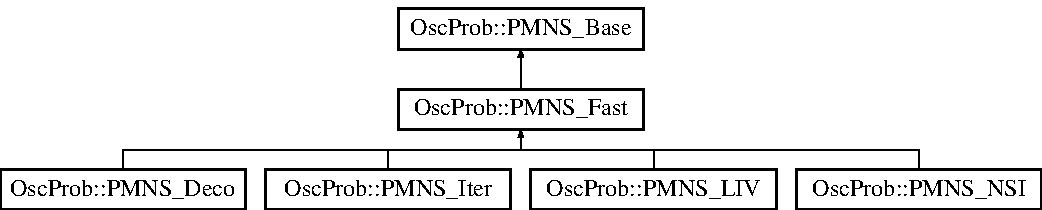
\includegraphics[height=2.818792cm]{classOscProb_1_1PMNS__Fast}
\end{center}
\end{figure}
\subsection*{Public Member Functions}
\begin{DoxyCompactItemize}
\item 
\hyperlink{classOscProb_1_1PMNS__Fast_a2bbac744bf63753105d766a860af7c0d}{P\+M\+N\+S\+\_\+\+Fast} ()
\begin{DoxyCompactList}\small\item\em Constructor. \end{DoxyCompactList}\item 
virtual \hyperlink{classOscProb_1_1PMNS__Fast_ae1b797dda260ff83793cdfe448f58878}{$\sim$\+P\+M\+N\+S\+\_\+\+Fast} ()
\begin{DoxyCompactList}\small\item\em Destructor. \end{DoxyCompactList}\item 
virtual void \hyperlink{classOscProb_1_1PMNS__Fast_ad849b2231d99c5d66fb3ade8efb896e1}{Set\+Mix} (double th12, double th23, double th13, double deltacp)
\begin{DoxyCompactList}\small\item\em Set the all mixing parameters at once. \end{DoxyCompactList}\item 
virtual void \hyperlink{classOscProb_1_1PMNS__Fast_a63733b246e6d2e609ce3de7a65ba5b9f}{Set\+Delta\+Msqrs} (double dm21, double dm32)
\begin{DoxyCompactList}\small\item\em Set both mass-\/splittings at once. \end{DoxyCompactList}\item 
virtual double \hyperlink{classOscProb_1_1PMNS__Base_aa2e10704d2d205a1ec8988de14b1a66f}{Prob} (std\+::vector$<$ \hyperlink{EigenPoint_8h_a67ca8e107e20610c3fff78d5e726ece0}{complexD} $>$ nu\+\_\+in, int flvf)
\begin{DoxyCompactList}\small\item\em Compute the probability of nu\+\_\+in going to flvf. \end{DoxyCompactList}\item 
virtual double \hyperlink{classOscProb_1_1PMNS__Base_a0190a79284289aacf682c78d7cef9a81}{Prob} (std\+::vector$<$ \hyperlink{EigenPoint_8h_a67ca8e107e20610c3fff78d5e726ece0}{complexD} $>$ nu\+\_\+in, int flvf, double E)
\begin{DoxyCompactList}\small\item\em Compute the probability of nu\+\_\+in going to flvf for energy E. \end{DoxyCompactList}\item 
virtual double \hyperlink{classOscProb_1_1PMNS__Base_a01fba31729345376705e02408e835f67}{Prob} (std\+::vector$<$ \hyperlink{EigenPoint_8h_a67ca8e107e20610c3fff78d5e726ece0}{complexD} $>$ nu\+\_\+in, int flvf, double E, double L)
\begin{DoxyCompactList}\small\item\em Compute the probability of nu\+\_\+in going to flvf for energy E and distance L. \end{DoxyCompactList}\item 
virtual double \hyperlink{classOscProb_1_1PMNS__Base_aec5c399b93261f1962a4b7dbbb44b973}{Prob} (int flvi, int flvf)
\begin{DoxyCompactList}\small\item\em Compute the probability of flvi going to flvf. \end{DoxyCompactList}\item 
virtual double \hyperlink{classOscProb_1_1PMNS__Base_aa3cee10639d5c0879ccb9e78d62128d3}{Prob} (int flvi, int flvf, double E)
\begin{DoxyCompactList}\small\item\em Compute the probability of flvi going to flvf for energy E. \end{DoxyCompactList}\item 
virtual double \hyperlink{classOscProb_1_1PMNS__Base_a6e0a74508d9d6db7be02e242b8467563}{Prob} (int flvi, int flvf, double E, double L)
\begin{DoxyCompactList}\small\item\em Compute the probability of flvi going to flvf for energy E and distance L. \end{DoxyCompactList}\item 
virtual double \hyperlink{classOscProb_1_1PMNS__Base_a89e54c80ae8a31effbab7b2b970606bb}{Avg\+Prob} (std\+::vector$<$ \hyperlink{EigenPoint_8h_a67ca8e107e20610c3fff78d5e726ece0}{complexD} $>$ nu\+\_\+in, int flvf, double E, double dE=0)
\begin{DoxyCompactList}\small\item\em Compute the average probability over a bin of energy. \end{DoxyCompactList}\item 
virtual double \hyperlink{classOscProb_1_1PMNS__Base_ac03f754160422e6600da8dbae0f803ed}{Avg\+Prob} (int flvi, int flvf, double E, double dE=0)
\begin{DoxyCompactList}\small\item\em Compute the average probability over a bin of energy. \end{DoxyCompactList}\item 
virtual double \hyperlink{classOscProb_1_1PMNS__Base_a19f160c045a01e5083506e925fb37d44}{Avg\+Prob\+LoE} (std\+::vector$<$ \hyperlink{EigenPoint_8h_a67ca8e107e20610c3fff78d5e726ece0}{complexD} $>$ nu\+\_\+in, int flvf, double LoE, double d\+LoE=0)
\begin{DoxyCompactList}\small\item\em Compute the average probability over a bin of L/E. \end{DoxyCompactList}\item 
virtual double \hyperlink{classOscProb_1_1PMNS__Base_ac19a92f4ef428a7333ca8eed76fca637}{Avg\+Prob\+LoE} (int flvi, int flvf, double LoE, double d\+LoE=0)
\begin{DoxyCompactList}\small\item\em Compute the average probability over a bin of L/E. \end{DoxyCompactList}\item 
virtual std\+::vector$<$ \hyperlink{EigenPoint_8h_a67ca8e107e20610c3fff78d5e726ece0}{complexD} $>$ \hyperlink{classOscProb_1_1PMNS__Base_a5092561dd8579d390c649eb60803ea98}{Get\+Mass\+Eigenstate} (int mi)
\begin{DoxyCompactList}\small\item\em Get a neutrino mass eigenstate. \end{DoxyCompactList}\item 
virtual void \hyperlink{classOscProb_1_1PMNS__Base_ace7875cf6d3bec161a2b7ed2690aec34}{Set\+Angle} (int i, int j, double th)
\begin{DoxyCompactList}\small\item\em Set the mixing angle theta\+\_\+ij. \end{DoxyCompactList}\item 
virtual void \hyperlink{classOscProb_1_1PMNS__Base_a4bef78cfcfc4e70b4ce79cdb8862c0a3}{Set\+Delta} (int i, int j, double delta)
\begin{DoxyCompactList}\small\item\em Set the CP phase delta\+\_\+ij. \end{DoxyCompactList}\item 
virtual void \hyperlink{classOscProb_1_1PMNS__Base_a492243b22fb1b783cd2943f507cff970}{Set\+Dm} (int j, double dm)
\begin{DoxyCompactList}\small\item\em Set the mass-\/splitting dm\+\_\+j1 in e\+V$^\wedge$2. \end{DoxyCompactList}\item 
virtual double \hyperlink{classOscProb_1_1PMNS__Base_acee137091304c919642293ddf015bbc8}{Get\+Angle} (int i, int j)
\begin{DoxyCompactList}\small\item\em Get the mixing angle theta\+\_\+ij. \end{DoxyCompactList}\item 
virtual double \hyperlink{classOscProb_1_1PMNS__Base_adb8dbc91d4286d2e7c8f768c59476241}{Get\+Delta} (int i, int j)
\begin{DoxyCompactList}\small\item\em Get the CP phase delta\+\_\+ij. \end{DoxyCompactList}\item 
virtual double \hyperlink{classOscProb_1_1PMNS__Base_ad26815ac5f4805d1259817e4936e5f8f}{Get\+Dm} (int j)
\begin{DoxyCompactList}\small\item\em Get the mass-\/splitting dm\+\_\+j1 in e\+V$^\wedge$2. \end{DoxyCompactList}\item 
virtual double \hyperlink{classOscProb_1_1PMNS__Base_a4ea861a6707ce1be3a54aad2b60f8632}{Get\+Dm\+Eff} (int j)
\begin{DoxyCompactList}\small\item\em Get the effective mass-\/splitting dm\+\_\+j1 in e\+V$^\wedge$2. \end{DoxyCompactList}\item 
virtual void \hyperlink{classOscProb_1_1PMNS__Base_a4de96ac9b6d1e9b029ab877e57d211ad}{Set\+Std\+Pars} ()
\begin{DoxyCompactList}\small\item\em Set P\+DG 3-\/flavor parameters. \end{DoxyCompactList}\item 
virtual void \hyperlink{classOscProb_1_1PMNS__Base_a95b3b0d0cab5e6a54b5ef99587f837c0}{Set\+Energy} (double E)
\begin{DoxyCompactList}\small\item\em Set the neutrino energy in GeV. \end{DoxyCompactList}\item 
virtual void \hyperlink{classOscProb_1_1PMNS__Base_a717e0348cf762f3961854e332a9b52e0}{Set\+Is\+Nu\+Bar} (bool is\+Nu\+Bar)
\begin{DoxyCompactList}\small\item\em Set the anti-\/neutrino flag. \end{DoxyCompactList}\item 
virtual double \hyperlink{classOscProb_1_1PMNS__Base_acc0d46cc4b8f911b40b807225003bbed}{Get\+Energy} ()
\begin{DoxyCompactList}\small\item\em Get the neutrino energy in GeV. \end{DoxyCompactList}\item 
virtual bool \hyperlink{classOscProb_1_1PMNS__Base_a2f7f2a028dfe7a90fff6b4f757972c2c}{Get\+Is\+Nu\+Bar} ()
\begin{DoxyCompactList}\small\item\em Get the anti-\/neutrino flag. \end{DoxyCompactList}\item 
virtual void \hyperlink{classOscProb_1_1PMNS__Base_ac3b644fd0a56347d304ceca4ae9d8875}{Set\+Path} (\hyperlink{structOscProb_1_1NuPath}{Osc\+Prob\+::\+Nu\+Path} p)
\begin{DoxyCompactList}\small\item\em Set a single path. \end{DoxyCompactList}\item 
virtual void \hyperlink{classOscProb_1_1PMNS__Base_a35b983270613072a3df58b574d80dbfd}{Set\+Path} (double length, double density, double zoa=0.\+5, int layer=0)
\begin{DoxyCompactList}\small\item\em Set a single path. \end{DoxyCompactList}\item 
virtual void \hyperlink{classOscProb_1_1PMNS__Base_a637d19dd850b4246507796526622643c}{Set\+Path} (std\+::vector$<$ \hyperlink{structOscProb_1_1NuPath}{Osc\+Prob\+::\+Nu\+Path} $>$ paths)
\begin{DoxyCompactList}\small\item\em Set a path sequence. \end{DoxyCompactList}\item 
virtual void \hyperlink{classOscProb_1_1PMNS__Base_a887dc9d4dc569ec0cdef3933b4c60efc}{Add\+Path} (\hyperlink{structOscProb_1_1NuPath}{Osc\+Prob\+::\+Nu\+Path} p)
\begin{DoxyCompactList}\small\item\em Add a path to the sequence. \end{DoxyCompactList}\item 
virtual void \hyperlink{classOscProb_1_1PMNS__Base_ab7f89ad9e7e1224adaa59d3c41594cd9}{Add\+Path} (double length, double density, double zoa=0.\+5, int layer=0)
\begin{DoxyCompactList}\small\item\em Add a path to the sequence. \end{DoxyCompactList}\item 
virtual void \hyperlink{classOscProb_1_1PMNS__Base_aefe521239031c418cfaaaa550a6e13bb}{Clear\+Path} ()
\begin{DoxyCompactList}\small\item\em Clear the path vector. \end{DoxyCompactList}\item 
virtual void \hyperlink{classOscProb_1_1PMNS__Base_a6241325b1bd28cafa556daaecbe4ed62}{Set\+Length} (double L)
\begin{DoxyCompactList}\small\item\em Set a single path lentgh in km. \end{DoxyCompactList}\item 
virtual void \hyperlink{classOscProb_1_1PMNS__Base_aa34a40a3b5abda0f252982d9ead3b520}{Set\+Length} (std\+::vector$<$ double $>$ L)
\begin{DoxyCompactList}\small\item\em Set multiple path lengths. \end{DoxyCompactList}\item 
virtual void \hyperlink{classOscProb_1_1PMNS__Base_ac74206f349687da141392c81e2ba6b0d}{Set\+Density} (double rho)
\begin{DoxyCompactList}\small\item\em Set single path density in g/cm$^\wedge$3. \end{DoxyCompactList}\item 
virtual void \hyperlink{classOscProb_1_1PMNS__Base_a858221d5510fe732dc6a101fd305cda0}{Set\+Density} (std\+::vector$<$ double $>$ rho)
\begin{DoxyCompactList}\small\item\em Set multiple path densities. \end{DoxyCompactList}\item 
virtual void \hyperlink{classOscProb_1_1PMNS__Base_a1bf3ea8fd2507fd2fd82d7410ff8f578}{Set\+ZoA} (double zoa)
\begin{DoxyCompactList}\small\item\em Set Z/A value for single path. \end{DoxyCompactList}\item 
virtual void \hyperlink{classOscProb_1_1PMNS__Base_a8495f8a320e1a21965e6a64aec92ad2a}{Set\+ZoA} (std\+::vector$<$ double $>$ zoa)
\begin{DoxyCompactList}\small\item\em Set multiple path Z/A values. \end{DoxyCompactList}\item 
virtual void \hyperlink{classOscProb_1_1PMNS__Base_a904e580edf89fb98bf9a6397739b4ebe}{Set\+Layers} (std\+::vector$<$ int $>$ lay)
\begin{DoxyCompactList}\small\item\em Set multiple path layer indices. \end{DoxyCompactList}\item 
virtual void \hyperlink{classOscProb_1_1PMNS__Base_add6533a9fc9acdfc7ae258b62570d78d}{Set\+Std\+Path} ()
\begin{DoxyCompactList}\small\item\em Set standard neutrino path. \end{DoxyCompactList}\item 
virtual std\+::vector$<$ \hyperlink{structOscProb_1_1NuPath}{Osc\+Prob\+::\+Nu\+Path} $>$ \hyperlink{classOscProb_1_1PMNS__Base_ac8e196f2e85a2b1caaf705073ee95a5c}{Get\+Path} ()
\begin{DoxyCompactList}\small\item\em Get the neutrino path sequence. \end{DoxyCompactList}\item 
virtual std\+::vector$<$ double $>$ \hyperlink{classOscProb_1_1PMNS__Base_a9eac8d768c1424755ee41f7e783af179}{Get\+Sample\+Points} (double LoE, double d\+LoE)
\begin{DoxyCompactList}\small\item\em Compute the sample points for a bin of L/E with width d\+LoE. \end{DoxyCompactList}\item 
virtual void \hyperlink{classOscProb_1_1PMNS__Base_aa94c1e1fff0ba731c75f7e633b023a9f}{Set\+Use\+Cache} (bool u=true)
\begin{DoxyCompactList}\small\item\em Set caching on/off. \end{DoxyCompactList}\item 
virtual void \hyperlink{classOscProb_1_1PMNS__Base_ac47fd33e69aa6490f99e2fd147a92f03}{Clear\+Cache} ()
\begin{DoxyCompactList}\small\item\em Clear the cache. \end{DoxyCompactList}\item 
virtual void \hyperlink{classOscProb_1_1PMNS__Base_ae67862cf58b0802487a14b047b012a78}{Set\+Max\+Cache} (int mc=1e6)
\begin{DoxyCompactList}\small\item\em Set max cache size. \end{DoxyCompactList}\end{DoxyCompactItemize}
\subsection*{Protected Member Functions}
\begin{DoxyCompactItemize}
\item 
virtual void \hyperlink{classOscProb_1_1PMNS__Fast_a16248082308f9d2c332ebf1be0aa90c3}{Update\+Ham} ()
\begin{DoxyCompactList}\small\item\em Build the full Hamiltonian. \end{DoxyCompactList}\item 
virtual void \hyperlink{classOscProb_1_1PMNS__Fast_a8a0828401591e88c60e0051fbfe02d5e}{Solve\+Ham} ()
\begin{DoxyCompactList}\small\item\em Solve the full Hamiltonian for eigenvectors and eigenvalues. \end{DoxyCompactList}\item 
virtual void \hyperlink{classOscProb_1_1PMNS__Fast_a76dd5a761df8689c502b28ad0391f9e2}{Set\+Vacuum\+Eigensystem} ()
\begin{DoxyCompactList}\small\item\em Set the eigensystem to the analytic solution of the vacuum Hamiltonian. \end{DoxyCompactList}\item 
virtual void \hyperlink{classOscProb_1_1PMNS__Base_adf23b569112f9f9e0e592f01d79a5f3d}{Initialize\+Vectors} ()
\begin{DoxyCompactList}\small\item\em Initialize all member vectors with zeros. \end{DoxyCompactList}\item 
virtual bool \hyperlink{classOscProb_1_1PMNS__Base_abe533da5f64bec1f4724ab7b58606b77}{Try\+Cache} ()
\begin{DoxyCompactList}\small\item\em Try to find a cached eigensystem. \end{DoxyCompactList}\item 
virtual void \hyperlink{classOscProb_1_1PMNS__Base_a785c37fcea974628623c8881bb0fbbf9}{Fill\+Cache} ()
\begin{DoxyCompactList}\small\item\em Cache the current eigensystem. \end{DoxyCompactList}\item 
virtual void \hyperlink{classOscProb_1_1PMNS__Base_a986e6ebef09a7e2eb7fee16a4c2c834d}{Set\+Cur\+Path} (\hyperlink{structOscProb_1_1NuPath}{Osc\+Prob\+::\+Nu\+Path} p)
\begin{DoxyCompactList}\small\item\em Set the path currently in use by the class. \end{DoxyCompactList}\item 
virtual void \hyperlink{classOscProb_1_1PMNS__Base_aba565962a440d14bee7a2a96d2eca2c5}{Set\+Att} (double att, int idx)
\begin{DoxyCompactList}\small\item\em Set one of the path attributes. \end{DoxyCompactList}\item 
virtual void \hyperlink{classOscProb_1_1PMNS__Base_aa001479b5f5828c3d16ed087f96ecbcc}{Set\+Att} (std\+::vector$<$ double $>$ att, int idx)
\begin{DoxyCompactList}\small\item\em Set all values of a path attribute. \end{DoxyCompactList}\item 
virtual void \hyperlink{classOscProb_1_1PMNS__Base_a6a3cf45bbe2349abf06708b65677c044}{RotateH} (int i, int j, std\+::vector$<$ std\+::vector$<$ \hyperlink{EigenPoint_8h_a67ca8e107e20610c3fff78d5e726ece0}{complexD} $>$ $>$ \&Ham)
\begin{DoxyCompactList}\small\item\em Rotate the Hamiltonian by theta\+\_\+ij and delta\+\_\+ij. \end{DoxyCompactList}\item 
virtual void \hyperlink{classOscProb_1_1PMNS__Base_ae52554477ad3250daa5adb8c32cab0b4}{Rotate\+State} (int i, int j)
\begin{DoxyCompactList}\small\item\em Rotate the neutrino state by theta\+\_\+ij and delta\+\_\+ij. \end{DoxyCompactList}\item 
virtual void \hyperlink{classOscProb_1_1PMNS__Base_ad0faf5eae755afb1baa1fcd5ffebad41}{Build\+Hms} ()
\begin{DoxyCompactList}\small\item\em Build the matrix of masses squared. \end{DoxyCompactList}\item 
virtual void \hyperlink{classOscProb_1_1PMNS__Base_ac0d4bf8ff1318ef96d3dafa62e0cec25}{Reset\+To\+Flavour} (int flv)
\begin{DoxyCompactList}\small\item\em Reset neutrino state to pure flavour flv. \end{DoxyCompactList}\item 
virtual void \hyperlink{classOscProb_1_1PMNS__Base_accb08503acc162188041d7a96a280462}{Propagate\+Path} (\hyperlink{structOscProb_1_1NuPath}{Osc\+Prob\+::\+Nu\+Path} p)
\begin{DoxyCompactList}\small\item\em Propagate neutrino through a single path. \end{DoxyCompactList}\item 
virtual void \hyperlink{classOscProb_1_1PMNS__Base_a054e3a8b05b9a958b6fa416e4a835e3e}{Propagate} ()
\begin{DoxyCompactList}\small\item\em Propagate neutrino through full path. \end{DoxyCompactList}\item 
virtual double \hyperlink{classOscProb_1_1PMNS__Base_a0dc4d45bc3d7e03b9abbf5b4e100cc22}{P} (int flv)
\begin{DoxyCompactList}\small\item\em Return the probability of final state in flavour flv. \end{DoxyCompactList}\end{DoxyCompactItemize}
\subsection*{Protected Attributes}
\begin{DoxyCompactItemize}
\item 
\hyperlink{EigenPoint_8h_a67ca8e107e20610c3fff78d5e726ece0}{complexD} \hyperlink{classOscProb_1_1PMNS__Fast_a94286a881bc53dd512a89d548346b611}{f\+Ham} \mbox{[}3\mbox{]}\mbox{[}3\mbox{]}
\begin{DoxyCompactList}\small\item\em The full hamiltonian. \end{DoxyCompactList}\item 
int \hyperlink{classOscProb_1_1PMNS__Base_a24bb74bed63569dfe88b18fa6a08060e}{f\+Num\+Nus}
\begin{DoxyCompactList}\small\item\em Number of neutrino flavours. \end{DoxyCompactList}\item 
std\+::vector$<$ double $>$ \hyperlink{classOscProb_1_1PMNS__Base_a406a31c3b5d620e5a0cace5b411f9f70}{f\+Dm}
\begin{DoxyCompactList}\small\item\em m$^\wedge$2\+\_\+i -\/ m$^\wedge$2\+\_\+1 in vacuum \end{DoxyCompactList}\item 
std\+::vector$<$ std\+::vector$<$ double $>$ $>$ \hyperlink{classOscProb_1_1PMNS__Base_a1976887cd658dd86b2336c181f1470b4}{f\+Theta}
\begin{DoxyCompactList}\small\item\em theta\mbox{[}i\mbox{]}\mbox{[}j\mbox{]} mixing angle \end{DoxyCompactList}\item 
std\+::vector$<$ std\+::vector$<$ double $>$ $>$ \hyperlink{classOscProb_1_1PMNS__Base_ab2a5fa40e689b221c8a7d2c17213810d}{f\+Delta}
\begin{DoxyCompactList}\small\item\em delta\mbox{[}i\mbox{]}\mbox{[}j\mbox{]} CP violating phase \end{DoxyCompactList}\item 
std\+::vector$<$ \hyperlink{EigenPoint_8h_a67ca8e107e20610c3fff78d5e726ece0}{complexD} $>$ \hyperlink{classOscProb_1_1PMNS__Base_abf99f2339e3ee989600740b5d88063e8}{f\+Nu\+State}
\begin{DoxyCompactList}\small\item\em The neutrino current state. \end{DoxyCompactList}\item 
std\+::vector$<$ std\+::vector$<$ \hyperlink{EigenPoint_8h_a67ca8e107e20610c3fff78d5e726ece0}{complexD} $>$ $>$ \hyperlink{classOscProb_1_1PMNS__Base_acd3c8783e7603081eab316ea4c86c766}{f\+Hms}
\begin{DoxyCompactList}\small\item\em matrix H$\ast$2E in e\+V$^\wedge$2 \end{DoxyCompactList}\item 
std\+::vector$<$ \hyperlink{EigenPoint_8h_a67ca8e107e20610c3fff78d5e726ece0}{complexD} $>$ \hyperlink{classOscProb_1_1PMNS__Base_ab8d26b722047d49d977f5f2d83026ede}{f\+Phases}
\begin{DoxyCompactList}\small\item\em Buffer for oscillation phases. \end{DoxyCompactList}\item 
std\+::vector$<$ \hyperlink{EigenPoint_8h_a67ca8e107e20610c3fff78d5e726ece0}{complexD} $>$ \hyperlink{classOscProb_1_1PMNS__Base_a5440bc3efa466a37649601abce559e3e}{f\+Buffer}
\begin{DoxyCompactList}\small\item\em Buffer for neutrino state tranformations. \end{DoxyCompactList}\item 
std\+::vector$<$ double $>$ \hyperlink{classOscProb_1_1PMNS__Base_a6319c34d7decbb9d7d6da279c06e8c2d}{f\+Eval}
\begin{DoxyCompactList}\small\item\em Eigenvalues of the Hamiltonian. \end{DoxyCompactList}\item 
std\+::vector$<$ std\+::vector$<$ \hyperlink{EigenPoint_8h_a67ca8e107e20610c3fff78d5e726ece0}{complexD} $>$ $>$ \hyperlink{classOscProb_1_1PMNS__Base_a87be137356c5f27ab83cab5e1298ef8f}{f\+Evec}
\begin{DoxyCompactList}\small\item\em Eigenvectors of the Hamiltonian. \end{DoxyCompactList}\item 
double \hyperlink{classOscProb_1_1PMNS__Base_a2800af6d436972f3e900867790c046b0}{f\+Energy}
\begin{DoxyCompactList}\small\item\em Neutrino energy. \end{DoxyCompactList}\item 
bool \hyperlink{classOscProb_1_1PMNS__Base_a0ebaeaefab36a3ff381c6293faedfdd6}{f\+Is\+Nu\+Bar}
\begin{DoxyCompactList}\small\item\em Anti-\/neutrino flag. \end{DoxyCompactList}\item 
std\+::vector$<$ \hyperlink{structOscProb_1_1NuPath}{Osc\+Prob\+::\+Nu\+Path} $>$ \hyperlink{classOscProb_1_1PMNS__Base_a69db9d57e12fc7cbe0431bc6c18fac93}{f\+Nu\+Paths}
\begin{DoxyCompactList}\small\item\em Vector of neutrino paths. \end{DoxyCompactList}\item 
\hyperlink{structOscProb_1_1NuPath}{Osc\+Prob\+::\+Nu\+Path} \hyperlink{classOscProb_1_1PMNS__Base_a849437aa8891fe042e86886ce8f81c6e}{f\+Path}
\begin{DoxyCompactList}\small\item\em Current neutrino path. \end{DoxyCompactList}\item 
bool \hyperlink{classOscProb_1_1PMNS__Base_a9ac3cadeac8db1b90f3152f476244780}{f\+Built\+Hms}
\begin{DoxyCompactList}\small\item\em Tag to avoid rebuilding Hms. \end{DoxyCompactList}\item 
bool \hyperlink{classOscProb_1_1PMNS__Base_a6dc5cd010d2d70b2324745b4e53e9839}{f\+Got\+ES}
\begin{DoxyCompactList}\small\item\em Tag to avoid recalculating eigensystem. \end{DoxyCompactList}\item 
bool \hyperlink{classOscProb_1_1PMNS__Base_ad28c12ef897b5555eda509ea55c99107}{f\+Use\+Cache}
\begin{DoxyCompactList}\small\item\em Flag for whether to use caching. \end{DoxyCompactList}\item 
double \hyperlink{classOscProb_1_1PMNS__Base_a0b4c41a27de281472453a1912cbc1e64}{f\+Cache\+Prec}
\begin{DoxyCompactList}\small\item\em Precision of cache matching. \end{DoxyCompactList}\item 
int \hyperlink{classOscProb_1_1PMNS__Base_a74c13356eafec2490d8c3c19759ba7f0}{f\+Max\+Cache}
\begin{DoxyCompactList}\small\item\em Maximum cache size. \end{DoxyCompactList}\item 
std\+::set$<$ \hyperlink{structOscProb_1_1EigenPoint}{Osc\+Prob\+::\+Eigen\+Point} $>$ \hyperlink{classOscProb_1_1PMNS__Base_a8159424f20197a3a7145fe3bf2c11176}{f\+Mix\+Cache}
\begin{DoxyCompactList}\small\item\em Caching set of eigensystems. \end{DoxyCompactList}\item 
\hyperlink{structOscProb_1_1EigenPoint}{Eigen\+Point} \hyperlink{classOscProb_1_1PMNS__Base_ab1fe4800ee3ae48df4fc942dce00e0d3}{f\+Probe}
\begin{DoxyCompactList}\small\item\em Eigenp\+Point to try. \end{DoxyCompactList}\end{DoxyCompactItemize}
\subsection*{Static Protected Attributes}
\begin{DoxyCompactItemize}
\item 
static const \hyperlink{EigenPoint_8h_a67ca8e107e20610c3fff78d5e726ece0}{complexD} \hyperlink{classOscProb_1_1PMNS__Base_a05e595848c2521dc795efa7645728b94}{zero}
\begin{DoxyCompactList}\small\item\em zero in complex \end{DoxyCompactList}\item 
static const \hyperlink{EigenPoint_8h_a67ca8e107e20610c3fff78d5e726ece0}{complexD} \hyperlink{classOscProb_1_1PMNS__Base_a7d1d0bbcab30a1fd8c368c40134c51ff}{one}
\begin{DoxyCompactList}\small\item\em one in complex \end{DoxyCompactList}\item 
static const double \hyperlink{classOscProb_1_1PMNS__Base_a382ddd7b76ca89b43f22614a2ea7327b}{k\+Km2eV} = 1.\+0 / 1.\+973269788e-\/10
\begin{DoxyCompactList}\small\item\em km to e\+V$^\wedge$-\/1 \end{DoxyCompactList}\item 
static const double \hyperlink{classOscProb_1_1PMNS__Base_a326fc5016d7dd7ce05682c06cdcb6d94}{k\+K2} = 1e-\/3 $\ast$ k\+N\+A / pow(k\+Km2e\+V,3)
\begin{DoxyCompactList}\small\item\em mol/\+Ge\+V$^\wedge$2/cm$^\wedge$3 to eV \end{DoxyCompactList}\item 
static const double \hyperlink{classOscProb_1_1PMNS__Base_ad36a0a6bf58d6ec093d3947784bd89e9}{k\+Ge\+V2eV} = 1.\+0e+09
\begin{DoxyCompactList}\small\item\em GeV to eV. \end{DoxyCompactList}\item 
static const double \hyperlink{classOscProb_1_1PMNS__Base_a69355e770b89e99437c2b8a66e48eeb9}{k\+NA} = 6.\+022140857e23
\begin{DoxyCompactList}\small\item\em Avogadro constant. \end{DoxyCompactList}\item 
static const double \hyperlink{classOscProb_1_1PMNS__Base_a7f26a3456128234b2ae6cc9141a6532f}{k\+Gf} = 1.\+1663787e-\/05
\begin{DoxyCompactList}\small\item\em G\+\_\+F in units of Ge\+V$^\wedge$-\/2. \end{DoxyCompactList}\end{DoxyCompactItemize}


\subsection{Detailed Description}
Two optimizations are relevant\+:~\newline

\begin{DoxyItemize}
\item The construction of the Hamiltonian avoids computing null terms~\newline

\item The eigensystem determination is based on the following reference\+:~\newline

\end{DoxyItemize}


\begin{DoxyPre}\end{DoxyPre}



\begin{DoxyPre}......................................................................\end{DoxyPre}



\begin{DoxyPre} Int. J. Mod. Phys. C       VOLUME 19, NUMBER 03            MARCH 2008\end{DoxyPre}



\begin{DoxyPre}     Efficient numerical diagonalization of hermitian 3x3 matrices\end{DoxyPre}



\begin{DoxyPre}                            Joachim Kopp
                  Max-Planck-Institut für Kernphysik 
             Postfach 10 39 80, 69029 Heidelberg, Germany
                    (Received 19 October 2007)\end{DoxyPre}



\begin{DoxyPre}                                523
......................................................................
 \end{DoxyPre}


\begin{DoxyAuthor}{Author}
Joao Coelho -\/ coelho@lal.\+in2p3.\+fr 
\end{DoxyAuthor}


Definition at line 38 of file P\+M\+N\+S\+\_\+\+Fast.\+h.



\subsection{Constructor \& Destructor Documentation}
\mbox{\Hypertarget{classOscProb_1_1PMNS__Fast_a2bbac744bf63753105d766a860af7c0d}\label{classOscProb_1_1PMNS__Fast_a2bbac744bf63753105d766a860af7c0d}} 
\index{Osc\+Prob\+::\+P\+M\+N\+S\+\_\+\+Fast@{Osc\+Prob\+::\+P\+M\+N\+S\+\_\+\+Fast}!P\+M\+N\+S\+\_\+\+Fast@{P\+M\+N\+S\+\_\+\+Fast}}
\index{P\+M\+N\+S\+\_\+\+Fast@{P\+M\+N\+S\+\_\+\+Fast}!Osc\+Prob\+::\+P\+M\+N\+S\+\_\+\+Fast@{Osc\+Prob\+::\+P\+M\+N\+S\+\_\+\+Fast}}
\subsubsection{\texorpdfstring{P\+M\+N\+S\+\_\+\+Fast()}{PMNS\_Fast()}}
{\footnotesize\ttfamily P\+M\+N\+S\+\_\+\+Fast\+::\+P\+M\+N\+S\+\_\+\+Fast (\begin{DoxyParamCaption}{ }\end{DoxyParamCaption})}

Constructor. \begin{DoxySeeAlso}{See also}
\hyperlink{classOscProb_1_1PMNS__Base_aa53e83b03a9cf4bdfa0a07136bd17a79}{P\+M\+N\+S\+\_\+\+Base\+::\+P\+M\+N\+S\+\_\+\+Base}
\end{DoxySeeAlso}
This class is restricted to 3 neutrino flavours. 

Definition at line 24 of file P\+M\+N\+S\+\_\+\+Fast.\+cxx.


\begin{DoxyCode}
24 : \hyperlink{classOscProb_1_1PMNS__Base_aa53e83b03a9cf4bdfa0a07136bd17a79}{PMNS\_Base}(), \hyperlink{classOscProb_1_1PMNS__Fast_a94286a881bc53dd512a89d548346b611}{fHam}() \{\}
\end{DoxyCode}
\mbox{\Hypertarget{classOscProb_1_1PMNS__Fast_ae1b797dda260ff83793cdfe448f58878}\label{classOscProb_1_1PMNS__Fast_ae1b797dda260ff83793cdfe448f58878}} 
\index{Osc\+Prob\+::\+P\+M\+N\+S\+\_\+\+Fast@{Osc\+Prob\+::\+P\+M\+N\+S\+\_\+\+Fast}!````~P\+M\+N\+S\+\_\+\+Fast@{$\sim$\+P\+M\+N\+S\+\_\+\+Fast}}
\index{````~P\+M\+N\+S\+\_\+\+Fast@{$\sim$\+P\+M\+N\+S\+\_\+\+Fast}!Osc\+Prob\+::\+P\+M\+N\+S\+\_\+\+Fast@{Osc\+Prob\+::\+P\+M\+N\+S\+\_\+\+Fast}}
\subsubsection{\texorpdfstring{$\sim$\+P\+M\+N\+S\+\_\+\+Fast()}{~PMNS\_Fast()}}
{\footnotesize\ttfamily P\+M\+N\+S\+\_\+\+Fast\+::$\sim$\+P\+M\+N\+S\+\_\+\+Fast (\begin{DoxyParamCaption}{ }\end{DoxyParamCaption})\hspace{0.3cm}{\ttfamily [virtual]}}

Nothing to clean. 

Definition at line 30 of file P\+M\+N\+S\+\_\+\+Fast.\+cxx.


\begin{DoxyCode}
30 \{\}
\end{DoxyCode}


\subsection{Member Function Documentation}
\mbox{\Hypertarget{classOscProb_1_1PMNS__Base_a887dc9d4dc569ec0cdef3933b4c60efc}\label{classOscProb_1_1PMNS__Base_a887dc9d4dc569ec0cdef3933b4c60efc}} 
\index{Osc\+Prob\+::\+P\+M\+N\+S\+\_\+\+Fast@{Osc\+Prob\+::\+P\+M\+N\+S\+\_\+\+Fast}!Add\+Path@{Add\+Path}}
\index{Add\+Path@{Add\+Path}!Osc\+Prob\+::\+P\+M\+N\+S\+\_\+\+Fast@{Osc\+Prob\+::\+P\+M\+N\+S\+\_\+\+Fast}}
\subsubsection{\texorpdfstring{Add\+Path()}{AddPath()}\hspace{0.1cm}{\footnotesize\ttfamily [1/2]}}
{\footnotesize\ttfamily void P\+M\+N\+S\+\_\+\+Base\+::\+Add\+Path (\begin{DoxyParamCaption}\item[{\hyperlink{structOscProb_1_1NuPath}{Osc\+Prob\+::\+Nu\+Path}}]{p }\end{DoxyParamCaption})\hspace{0.3cm}{\ttfamily [virtual]}, {\ttfamily [inherited]}}

Add a path to the sequence. 
\begin{DoxyParams}{Parameters}
{\em p} & -\/ A neutrino path segment \\
\hline
\end{DoxyParams}


Definition at line 351 of file P\+M\+N\+S\+\_\+\+Base.\+cxx.



References Osc\+Prob\+::\+P\+M\+N\+S\+\_\+\+Base\+::f\+Nu\+Paths.



Referenced by Osc\+Prob\+::\+P\+M\+N\+S\+\_\+\+Base\+::\+Add\+Path(), Osc\+Prob\+::\+P\+M\+N\+S\+\_\+\+Base\+::\+Set\+Att(), and Osc\+Prob\+::\+P\+M\+N\+S\+\_\+\+Base\+::\+Set\+Path().


\begin{DoxyCode}
351                                \{
352 
353   \hyperlink{classOscProb_1_1PMNS__Base_a69db9d57e12fc7cbe0431bc6c18fac93}{fNuPaths}.push\_back(p);
354 
355 \}
\end{DoxyCode}
\mbox{\Hypertarget{classOscProb_1_1PMNS__Base_ab7f89ad9e7e1224adaa59d3c41594cd9}\label{classOscProb_1_1PMNS__Base_ab7f89ad9e7e1224adaa59d3c41594cd9}} 
\index{Osc\+Prob\+::\+P\+M\+N\+S\+\_\+\+Fast@{Osc\+Prob\+::\+P\+M\+N\+S\+\_\+\+Fast}!Add\+Path@{Add\+Path}}
\index{Add\+Path@{Add\+Path}!Osc\+Prob\+::\+P\+M\+N\+S\+\_\+\+Fast@{Osc\+Prob\+::\+P\+M\+N\+S\+\_\+\+Fast}}
\subsubsection{\texorpdfstring{Add\+Path()}{AddPath()}\hspace{0.1cm}{\footnotesize\ttfamily [2/2]}}
{\footnotesize\ttfamily void P\+M\+N\+S\+\_\+\+Base\+::\+Add\+Path (\begin{DoxyParamCaption}\item[{double}]{length,  }\item[{double}]{density,  }\item[{double}]{zoa = {\ttfamily 0.5},  }\item[{int}]{layer = {\ttfamily 0} }\end{DoxyParamCaption})\hspace{0.3cm}{\ttfamily [virtual]}, {\ttfamily [inherited]}}

Add a path to the sequence defining attributes directly. 
\begin{DoxyParams}{Parameters}
{\em length} & -\/ The length of the path segment in km \\
\hline
{\em density} & -\/ The density of the path segment in g/cm$^\wedge$3 \\
\hline
{\em zoa} & -\/ The effective Z/A of the path segment \\
\hline
{\em layer} & -\/ An index to identify the layer type (e.\+g. earth inner core) \\
\hline
\end{DoxyParams}


Definition at line 365 of file P\+M\+N\+S\+\_\+\+Base.\+cxx.



References Osc\+Prob\+::\+P\+M\+N\+S\+\_\+\+Base\+::\+Add\+Path().


\begin{DoxyCode}
365                                                                            \{
366 
367   \hyperlink{classOscProb_1_1PMNS__Base_a887dc9d4dc569ec0cdef3933b4c60efc}{AddPath}(\hyperlink{structOscProb_1_1NuPath}{NuPath}(length, density, zoa, layer));
368 
369 \}
\end{DoxyCode}
\mbox{\Hypertarget{classOscProb_1_1PMNS__Base_a89e54c80ae8a31effbab7b2b970606bb}\label{classOscProb_1_1PMNS__Base_a89e54c80ae8a31effbab7b2b970606bb}} 
\index{Osc\+Prob\+::\+P\+M\+N\+S\+\_\+\+Fast@{Osc\+Prob\+::\+P\+M\+N\+S\+\_\+\+Fast}!Avg\+Prob@{Avg\+Prob}}
\index{Avg\+Prob@{Avg\+Prob}!Osc\+Prob\+::\+P\+M\+N\+S\+\_\+\+Fast@{Osc\+Prob\+::\+P\+M\+N\+S\+\_\+\+Fast}}
\subsubsection{\texorpdfstring{Avg\+Prob()}{AvgProb()}\hspace{0.1cm}{\footnotesize\ttfamily [1/2]}}
{\footnotesize\ttfamily double P\+M\+N\+S\+\_\+\+Base\+::\+Avg\+Prob (\begin{DoxyParamCaption}\item[{std\+::vector$<$ \hyperlink{EigenPoint_8h_a67ca8e107e20610c3fff78d5e726ece0}{complexD} $>$}]{nu\+\_\+in,  }\item[{int}]{flvf,  }\item[{double}]{E,  }\item[{double}]{dE = {\ttfamily 0} }\end{DoxyParamCaption})\hspace{0.3cm}{\ttfamily [virtual]}, {\ttfamily [inherited]}}

Compute the average probability of nu\+\_\+in going to flvf over a bin of energy E with width dE.

This gets transformed into L/E, since the oscillation terms have arguments linear in L/E and not E.

This function works best for single paths. In multiple paths the accuracy may be somewhat worse. If needed, average over smaller energy ranges.

Flavours are\+: 
\begin{DoxyPre}
  0 = nue, 1 = numu, 2 = nutau
  3 = sterile\_1, 4 = sterile\_2, etc.
\end{DoxyPre}
 
\begin{DoxyParams}{Parameters}
{\em nu\+\_\+in} & -\/ The neutrino initial state in flavour. \\
\hline
{\em flvf} & -\/ The neutrino final flavour. \\
\hline
{\em E} & -\/ The neutrino energy in the bin center in GeV \\
\hline
{\em dE} & -\/ The energy bin width in GeV\\
\hline
\end{DoxyParams}
\begin{DoxyReturn}{Returns}
Average neutrino oscillation probability 
\end{DoxyReturn}


Definition at line 1386 of file P\+M\+N\+S\+\_\+\+Base.\+cxx.



References Osc\+Prob\+::\+Avg\+Path(), Osc\+Prob\+::\+P\+M\+N\+S\+\_\+\+Base\+::\+Avg\+Prob\+Lo\+E(), Osc\+Prob\+::\+P\+M\+N\+S\+\_\+\+Base\+::f\+Nu\+Paths, Osc\+Prob\+::\+P\+M\+N\+S\+\_\+\+Base\+::f\+Path, Osc\+Prob\+::\+Nu\+Path\+::length, Osc\+Prob\+::\+P\+M\+N\+S\+\_\+\+Base\+::\+Prob(), and Osc\+Prob\+::\+P\+M\+N\+S\+\_\+\+Base\+::\+Set\+Cur\+Path().



Referenced by Osc\+Prob\+::\+P\+M\+N\+S\+\_\+\+Base\+::\+Avg\+Prob().


\begin{DoxyCode}
1387 \{
1388 
1389   \textcolor{comment}{// Do nothing if energy is not positive}
1390   \textcolor{keywordflow}{if}(E<=0) \textcolor{keywordflow}{return} 0;
1391 
1392   \textcolor{keywordflow}{if}(\hyperlink{classOscProb_1_1PMNS__Base_a69db9d57e12fc7cbe0431bc6c18fac93}{fNuPaths}.empty()) \textcolor{keywordflow}{return} 0;
1393 
1394   \textcolor{comment}{// Don't average zero width}
1395   \textcolor{keywordflow}{if}(dE<=0) \textcolor{keywordflow}{return} \hyperlink{classOscProb_1_1PMNS__Base_aa2e10704d2d205a1ec8988de14b1a66f}{Prob}(nu\_in, flvf, E);
1396 
1397   \textcolor{comment}{// Make sure fPath is set}
1398   \textcolor{comment}{// Use average if multiple paths}
1399   \hyperlink{classOscProb_1_1PMNS__Base_a986e6ebef09a7e2eb7fee16a4c2c834d}{SetCurPath}(\hyperlink{namespaceOscProb_a999a7944bad8bc72d7ee9f56f81a210e}{AvgPath}(\hyperlink{classOscProb_1_1PMNS__Base_a69db9d57e12fc7cbe0431bc6c18fac93}{fNuPaths}));
1400 
1401   \textcolor{comment}{// Define L/E variables}
1402   \textcolor{keywordtype}{double} LoE = 0;
1403   \textcolor{keywordtype}{double} dLoE = 0;
1404 
1405   \textcolor{comment}{// Set a minimum energy}
1406   \textcolor{keywordtype}{double} minE = 0.1 * E;
1407 
1408   \textcolor{comment}{// Transform range to L/E}
1409   \textcolor{comment}{// Full range if low edge > minE}
1410   \textcolor{keywordflow}{if}(E-dE/2 > minE)\{
1411     LoE = 0.5 * (\hyperlink{classOscProb_1_1PMNS__Base_a849437aa8891fe042e86886ce8f81c6e}{fPath}.\hyperlink{structOscProb_1_1NuPath_af22660894b6e25cf835500381b155557}{length}/(E-dE/2) + \hyperlink{classOscProb_1_1PMNS__Base_a849437aa8891fe042e86886ce8f81c6e}{fPath}.\hyperlink{structOscProb_1_1NuPath_af22660894b6e25cf835500381b155557}{length}/(E+dE/2));
1412     dLoE = \hyperlink{classOscProb_1_1PMNS__Base_a849437aa8891fe042e86886ce8f81c6e}{fPath}.\hyperlink{structOscProb_1_1NuPath_af22660894b6e25cf835500381b155557}{length}/(E-dE/2) - \hyperlink{classOscProb_1_1PMNS__Base_a849437aa8891fe042e86886ce8f81c6e}{fPath}.\hyperlink{structOscProb_1_1NuPath_af22660894b6e25cf835500381b155557}{length}/(E+dE/2);
1413   \}
1414   \textcolor{comment}{// Else start at minE}
1415   \textcolor{keywordflow}{else}\{
1416     LoE = 0.5 * (\hyperlink{classOscProb_1_1PMNS__Base_a849437aa8891fe042e86886ce8f81c6e}{fPath}.\hyperlink{structOscProb_1_1NuPath_af22660894b6e25cf835500381b155557}{length}/minE + \hyperlink{classOscProb_1_1PMNS__Base_a849437aa8891fe042e86886ce8f81c6e}{fPath}.\hyperlink{structOscProb_1_1NuPath_af22660894b6e25cf835500381b155557}{length}/(E+dE/2));
1417     dLoE = \hyperlink{classOscProb_1_1PMNS__Base_a849437aa8891fe042e86886ce8f81c6e}{fPath}.\hyperlink{structOscProb_1_1NuPath_af22660894b6e25cf835500381b155557}{length}/minE - \hyperlink{classOscProb_1_1PMNS__Base_a849437aa8891fe042e86886ce8f81c6e}{fPath}.\hyperlink{structOscProb_1_1NuPath_af22660894b6e25cf835500381b155557}{length}/(E+dE/2);
1418   \}
1419 
1420   \textcolor{comment}{// Compute average in LoE}
1421   \textcolor{keywordflow}{return} \hyperlink{classOscProb_1_1PMNS__Base_a19f160c045a01e5083506e925fb37d44}{AvgProbLoE}(nu\_in, flvf, LoE, dLoE);
1422 
1423 \}
\end{DoxyCode}
\mbox{\Hypertarget{classOscProb_1_1PMNS__Base_ac03f754160422e6600da8dbae0f803ed}\label{classOscProb_1_1PMNS__Base_ac03f754160422e6600da8dbae0f803ed}} 
\index{Osc\+Prob\+::\+P\+M\+N\+S\+\_\+\+Fast@{Osc\+Prob\+::\+P\+M\+N\+S\+\_\+\+Fast}!Avg\+Prob@{Avg\+Prob}}
\index{Avg\+Prob@{Avg\+Prob}!Osc\+Prob\+::\+P\+M\+N\+S\+\_\+\+Fast@{Osc\+Prob\+::\+P\+M\+N\+S\+\_\+\+Fast}}
\subsubsection{\texorpdfstring{Avg\+Prob()}{AvgProb()}\hspace{0.1cm}{\footnotesize\ttfamily [2/2]}}
{\footnotesize\ttfamily double P\+M\+N\+S\+\_\+\+Base\+::\+Avg\+Prob (\begin{DoxyParamCaption}\item[{int}]{flvi,  }\item[{int}]{flvf,  }\item[{double}]{E,  }\item[{double}]{dE = {\ttfamily 0} }\end{DoxyParamCaption})\hspace{0.3cm}{\ttfamily [virtual]}, {\ttfamily [inherited]}}

Compute the average probability of flvi going to flvf over a bin of energy E with width dE.

This gets transformed into L/E, since the oscillation terms have arguments linear in L/E and not E.

This function works best for single paths. In multiple paths the accuracy may be somewhat worse. If needed, average over smaller energy ranges.

Flavours are\+: 
\begin{DoxyPre}
  0 = nue, 1 = numu, 2 = nutau
  3 = sterile\_1, 4 = sterile\_2, etc.
\end{DoxyPre}
 
\begin{DoxyParams}{Parameters}
{\em flvi} & -\/ The neutrino starting flavour. \\
\hline
{\em flvf} & -\/ The neutrino final flavour. \\
\hline
{\em E} & -\/ The neutrino energy in the bin center in GeV \\
\hline
{\em dE} & -\/ The energy bin width in GeV\\
\hline
\end{DoxyParams}
\begin{DoxyReturn}{Returns}
Average neutrino oscillation probability 
\end{DoxyReturn}


Definition at line 1353 of file P\+M\+N\+S\+\_\+\+Base.\+cxx.



References Osc\+Prob\+::\+P\+M\+N\+S\+\_\+\+Base\+::\+Avg\+Prob(), Osc\+Prob\+::\+P\+M\+N\+S\+\_\+\+Base\+::f\+Nu\+State, and Osc\+Prob\+::\+P\+M\+N\+S\+\_\+\+Base\+::\+Reset\+To\+Flavour().


\begin{DoxyCode}
1354 \{
1355 
1356   \hyperlink{classOscProb_1_1PMNS__Base_ac0d4bf8ff1318ef96d3dafa62e0cec25}{ResetToFlavour}(flvi);
1357 
1358   \textcolor{keywordflow}{return} \hyperlink{classOscProb_1_1PMNS__Base_a89e54c80ae8a31effbab7b2b970606bb}{AvgProb}(\hyperlink{classOscProb_1_1PMNS__Base_abf99f2339e3ee989600740b5d88063e8}{fNuState}, flvf, E, dE);
1359 
1360 \}
\end{DoxyCode}
\mbox{\Hypertarget{classOscProb_1_1PMNS__Base_a19f160c045a01e5083506e925fb37d44}\label{classOscProb_1_1PMNS__Base_a19f160c045a01e5083506e925fb37d44}} 
\index{Osc\+Prob\+::\+P\+M\+N\+S\+\_\+\+Fast@{Osc\+Prob\+::\+P\+M\+N\+S\+\_\+\+Fast}!Avg\+Prob\+LoE@{Avg\+Prob\+LoE}}
\index{Avg\+Prob\+LoE@{Avg\+Prob\+LoE}!Osc\+Prob\+::\+P\+M\+N\+S\+\_\+\+Fast@{Osc\+Prob\+::\+P\+M\+N\+S\+\_\+\+Fast}}
\subsubsection{\texorpdfstring{Avg\+Prob\+Lo\+E()}{AvgProbLoE()}\hspace{0.1cm}{\footnotesize\ttfamily [1/2]}}
{\footnotesize\ttfamily double P\+M\+N\+S\+\_\+\+Base\+::\+Avg\+Prob\+LoE (\begin{DoxyParamCaption}\item[{std\+::vector$<$ \hyperlink{EigenPoint_8h_a67ca8e107e20610c3fff78d5e726ece0}{complexD} $>$}]{nu\+\_\+in,  }\item[{int}]{flvf,  }\item[{double}]{LoE,  }\item[{double}]{d\+LoE = {\ttfamily 0} }\end{DoxyParamCaption})\hspace{0.3cm}{\ttfamily [virtual]}, {\ttfamily [inherited]}}

Compute the average probability of nu\+\_\+in going to flvf over a bin of L/E with width d\+LoE.

The probabilities are weighted by (L/E)$^\wedge$-\/2 so that event density is flat in energy. This avoids giving too much weight to low energies. Better approximations would be achieved if we used an interpolated event density.

This function works best for single paths. In multiple paths the accuracy may be somewhat worse. If needed, average over smaller L/E ranges.

Flavours are\+: 
\begin{DoxyPre}
  0 = nue, 1 = numu, 2 = nutau
  3 = sterile\_1, 4 = sterile\_2, etc.
\end{DoxyPre}
 
\begin{DoxyParams}{Parameters}
{\em nu\+\_\+in} & -\/ The neutrino intial state in flavour basis. \\
\hline
{\em flvf} & -\/ The neutrino final flavour. \\
\hline
{\em LoE} & -\/ The neutrino L/E value in the bin center in km/\+GeV \\
\hline
{\em d\+LoE} & -\/ The L/E bin width in km/\+GeV\\
\hline
\end{DoxyParams}
\begin{DoxyReturn}{Returns}
Average neutrino oscillation probability 
\end{DoxyReturn}


Definition at line 1486 of file P\+M\+N\+S\+\_\+\+Base.\+cxx.



References Osc\+Prob\+::\+Avg\+Path(), Osc\+Prob\+::\+P\+M\+N\+S\+\_\+\+Base\+::f\+Nu\+Paths, Osc\+Prob\+::\+P\+M\+N\+S\+\_\+\+Base\+::f\+Path, Osc\+Prob\+::\+P\+M\+N\+S\+\_\+\+Base\+::\+Get\+Sample\+Points(), Osc\+Prob\+::\+Nu\+Path\+::length, Osc\+Prob\+::\+P\+M\+N\+S\+\_\+\+Base\+::\+Prob(), Osc\+Prob\+::\+P\+M\+N\+S\+\_\+\+Base\+::\+Set\+Cur\+Path(), and Osc\+Prob\+::\+P\+M\+N\+S\+\_\+\+Base\+::\+Set\+Energy().



Referenced by Osc\+Prob\+::\+P\+M\+N\+S\+\_\+\+Base\+::\+Avg\+Prob(), and Osc\+Prob\+::\+P\+M\+N\+S\+\_\+\+Base\+::\+Avg\+Prob\+Lo\+E().


\begin{DoxyCode}
1487 \{
1488 
1489   \textcolor{comment}{// Do nothing if L/E is not positive}
1490   \textcolor{keywordflow}{if}(LoE<=0) \textcolor{keywordflow}{return} 0;
1491 
1492   \textcolor{keywordflow}{if}(\hyperlink{classOscProb_1_1PMNS__Base_a69db9d57e12fc7cbe0431bc6c18fac93}{fNuPaths}.empty()) \textcolor{keywordflow}{return} 0;
1493 
1494   \textcolor{comment}{// Make sure fPath is set}
1495   \textcolor{comment}{// Use average if multiple paths}
1496   \hyperlink{classOscProb_1_1PMNS__Base_a986e6ebef09a7e2eb7fee16a4c2c834d}{SetCurPath}(\hyperlink{namespaceOscProb_a999a7944bad8bc72d7ee9f56f81a210e}{AvgPath}(\hyperlink{classOscProb_1_1PMNS__Base_a69db9d57e12fc7cbe0431bc6c18fac93}{fNuPaths}));
1497 
1498   \textcolor{comment}{// Set the energy at bin center}
1499   \hyperlink{classOscProb_1_1PMNS__Base_a95b3b0d0cab5e6a54b5ef99587f837c0}{SetEnergy}(\hyperlink{classOscProb_1_1PMNS__Base_a849437aa8891fe042e86886ce8f81c6e}{fPath}.\hyperlink{structOscProb_1_1NuPath_af22660894b6e25cf835500381b155557}{length}/LoE);
1500 
1501   \textcolor{comment}{// Don't average zero width}
1502   \textcolor{keywordflow}{if}(dLoE<=0) \textcolor{keywordflow}{return} \hyperlink{classOscProb_1_1PMNS__Base_aa2e10704d2d205a1ec8988de14b1a66f}{Prob}(nu\_in, flvf);
1503 
1504   \textcolor{comment}{// Get sample points for this bin}
1505   vector<double> samples = \hyperlink{classOscProb_1_1PMNS__Base_a9eac8d768c1424755ee41f7e783af179}{GetSamplePoints}(LoE, dLoE);
1506 
1507   \textcolor{comment}{// Variables to fill sample}
1508   \textcolor{comment}{// probabilities and weights}
1509   \textcolor{keywordtype}{double} sumw = 0;
1510   \textcolor{keywordtype}{double} prob = 0;
1511   \textcolor{keywordtype}{double} length = \hyperlink{classOscProb_1_1PMNS__Base_a849437aa8891fe042e86886ce8f81c6e}{fPath}.\hyperlink{structOscProb_1_1NuPath_af22660894b6e25cf835500381b155557}{length};
1512 
1513   \textcolor{comment}{// Loop over all sample points}
1514   \textcolor{keywordflow}{for}(\textcolor{keywordtype}{int} j=0; j<int(samples.size()); j++)\{
1515 
1516     \textcolor{comment}{// Set (L/E)^-2 weights}
1517     \textcolor{keywordtype}{double} w = 1./pow(samples[j],2);
1518 
1519     \textcolor{comment}{// Add weighted probability}
1520     prob += w * \hyperlink{classOscProb_1_1PMNS__Base_aa2e10704d2d205a1ec8988de14b1a66f}{Prob}(nu\_in, flvf, length / samples[j]);
1521 
1522     \textcolor{comment}{// Increment sum of weights}
1523     sumw += w;
1524 
1525   \}
1526 
1527   \textcolor{comment}{// Return weighted average of probabilities}
1528   \textcolor{keywordflow}{return} prob / sumw;
1529 
1530 \}
\end{DoxyCode}
\mbox{\Hypertarget{classOscProb_1_1PMNS__Base_ac19a92f4ef428a7333ca8eed76fca637}\label{classOscProb_1_1PMNS__Base_ac19a92f4ef428a7333ca8eed76fca637}} 
\index{Osc\+Prob\+::\+P\+M\+N\+S\+\_\+\+Fast@{Osc\+Prob\+::\+P\+M\+N\+S\+\_\+\+Fast}!Avg\+Prob\+LoE@{Avg\+Prob\+LoE}}
\index{Avg\+Prob\+LoE@{Avg\+Prob\+LoE}!Osc\+Prob\+::\+P\+M\+N\+S\+\_\+\+Fast@{Osc\+Prob\+::\+P\+M\+N\+S\+\_\+\+Fast}}
\subsubsection{\texorpdfstring{Avg\+Prob\+Lo\+E()}{AvgProbLoE()}\hspace{0.1cm}{\footnotesize\ttfamily [2/2]}}
{\footnotesize\ttfamily double P\+M\+N\+S\+\_\+\+Base\+::\+Avg\+Prob\+LoE (\begin{DoxyParamCaption}\item[{int}]{flvi,  }\item[{int}]{flvf,  }\item[{double}]{LoE,  }\item[{double}]{d\+LoE = {\ttfamily 0} }\end{DoxyParamCaption})\hspace{0.3cm}{\ttfamily [virtual]}, {\ttfamily [inherited]}}

Compute the average probability of flvi going to flvf over a bin of L/E with width d\+LoE.

The probabilities are weighted by (L/E)$^\wedge$-\/2 so that event density is flat in energy. This avoids giving too much weight to low energies. Better approximations would be achieved if we used an interpolated event density.

This function works best for single paths. In multiple paths the accuracy may be somewhat worse. If needed, average over smaller L/E ranges.

Flavours are\+: 
\begin{DoxyPre}
  0 = nue, 1 = numu, 2 = nutau
  3 = sterile\_1, 4 = sterile\_2, etc.
\end{DoxyPre}
 
\begin{DoxyParams}{Parameters}
{\em flvi} & -\/ The neutrino starting flavour. \\
\hline
{\em flvf} & -\/ The neutrino final flavour. \\
\hline
{\em LoE} & -\/ The neutrino L/E value in the bin center in km/\+GeV \\
\hline
{\em d\+LoE} & -\/ The L/E bin width in km/\+GeV\\
\hline
\end{DoxyParams}
\begin{DoxyReturn}{Returns}
Average neutrino oscillation probability 
\end{DoxyReturn}


Definition at line 1451 of file P\+M\+N\+S\+\_\+\+Base.\+cxx.



References Osc\+Prob\+::\+P\+M\+N\+S\+\_\+\+Base\+::\+Avg\+Prob\+Lo\+E(), Osc\+Prob\+::\+P\+M\+N\+S\+\_\+\+Base\+::f\+Nu\+State, and Osc\+Prob\+::\+P\+M\+N\+S\+\_\+\+Base\+::\+Reset\+To\+Flavour().


\begin{DoxyCode}
1452 \{
1453 
1454   \hyperlink{classOscProb_1_1PMNS__Base_ac0d4bf8ff1318ef96d3dafa62e0cec25}{ResetToFlavour}(flvi);
1455 
1456   \textcolor{keywordflow}{return} \hyperlink{classOscProb_1_1PMNS__Base_a19f160c045a01e5083506e925fb37d44}{AvgProbLoE}(\hyperlink{classOscProb_1_1PMNS__Base_abf99f2339e3ee989600740b5d88063e8}{fNuState}, flvf, LoE, dLoE);
1457 
1458 \}
\end{DoxyCode}
\mbox{\Hypertarget{classOscProb_1_1PMNS__Base_ad0faf5eae755afb1baa1fcd5ffebad41}\label{classOscProb_1_1PMNS__Base_ad0faf5eae755afb1baa1fcd5ffebad41}} 
\index{Osc\+Prob\+::\+P\+M\+N\+S\+\_\+\+Fast@{Osc\+Prob\+::\+P\+M\+N\+S\+\_\+\+Fast}!Build\+Hms@{Build\+Hms}}
\index{Build\+Hms@{Build\+Hms}!Osc\+Prob\+::\+P\+M\+N\+S\+\_\+\+Fast@{Osc\+Prob\+::\+P\+M\+N\+S\+\_\+\+Fast}}
\subsubsection{\texorpdfstring{Build\+Hms()}{BuildHms()}}
{\footnotesize\ttfamily void P\+M\+N\+S\+\_\+\+Base\+::\+Build\+Hms (\begin{DoxyParamCaption}{ }\end{DoxyParamCaption})\hspace{0.3cm}{\ttfamily [protected]}, {\ttfamily [virtual]}, {\ttfamily [inherited]}}

Build Hms = H$\ast$2E, where H is the Hamiltonian in vacuum on flavour basis and E is the neutrino energy in eV. Hms is effectively the matrix of masses squared.

This is a hermitian matrix, so only the upper triangular part needs to be filled

The construction of the Hamiltonian avoids computing terms that are simply zero. This has a big impact in the computation time. 

Definition at line 1045 of file P\+M\+N\+S\+\_\+\+Base.\+cxx.



References Osc\+Prob\+::\+P\+M\+N\+S\+\_\+\+Base\+::\+Clear\+Cache(), Osc\+Prob\+::\+P\+M\+N\+S\+\_\+\+Base\+::f\+Built\+Hms, Osc\+Prob\+::\+P\+M\+N\+S\+\_\+\+Base\+::f\+Dm, Osc\+Prob\+::\+P\+M\+N\+S\+\_\+\+Base\+::f\+Got\+ES, Osc\+Prob\+::\+P\+M\+N\+S\+\_\+\+Base\+::f\+Hms, Osc\+Prob\+::\+P\+M\+N\+S\+\_\+\+Base\+::f\+Num\+Nus, and Osc\+Prob\+::\+P\+M\+N\+S\+\_\+\+Base\+::\+Rotate\+H().



Referenced by Osc\+Prob\+::\+P\+M\+N\+S\+\_\+\+Sterile\+::\+Solve\+Ham(), and Solve\+Ham().


\begin{DoxyCode}
1046 \{
1047 
1048   \textcolor{comment}{// Check if anything changed}
1049   \textcolor{keywordflow}{if}(\hyperlink{classOscProb_1_1PMNS__Base_a9ac3cadeac8db1b90f3152f476244780}{fBuiltHms}) \textcolor{keywordflow}{return};
1050   
1051   \textcolor{comment}{// Tag to recompute eigensystem}
1052   \hyperlink{classOscProb_1_1PMNS__Base_a6dc5cd010d2d70b2324745b4e53e9839}{fGotES} = \textcolor{keyword}{false};
1053 
1054   \textcolor{keywordflow}{for}(\textcolor{keywordtype}{int} j=0; j<\hyperlink{classOscProb_1_1PMNS__Base_a24bb74bed63569dfe88b18fa6a08060e}{fNumNus}; j++)\{
1055     \textcolor{comment}{// Set mass splitting}
1056     \hyperlink{classOscProb_1_1PMNS__Base_acd3c8783e7603081eab316ea4c86c766}{fHms}[j][j] = \hyperlink{classOscProb_1_1PMNS__Base_a406a31c3b5d620e5a0cace5b411f9f70}{fDm}[j];
1057     \textcolor{comment}{// Reset off-diagonal elements}
1058     \textcolor{keywordflow}{for}(\textcolor{keywordtype}{int} i=0; i<j; i++)\{
1059       \hyperlink{classOscProb_1_1PMNS__Base_acd3c8783e7603081eab316ea4c86c766}{fHms}[i][j] = 0;
1060     \}
1061     \textcolor{comment}{// Rotate j neutrinos}
1062     \textcolor{keywordflow}{for}(\textcolor{keywordtype}{int} i=0; i<j; i++)\{
1063       \hyperlink{classOscProb_1_1PMNS__Base_a6a3cf45bbe2349abf06708b65677c044}{RotateH}(i,j,\hyperlink{classOscProb_1_1PMNS__Base_acd3c8783e7603081eab316ea4c86c766}{fHms});
1064     \}
1065   \}
1066 
1067   \hyperlink{classOscProb_1_1PMNS__Base_ac47fd33e69aa6490f99e2fd147a92f03}{ClearCache}();
1068 
1069   \textcolor{comment}{// Tag as built}
1070   \hyperlink{classOscProb_1_1PMNS__Base_a9ac3cadeac8db1b90f3152f476244780}{fBuiltHms} = \textcolor{keyword}{true};
1071 
1072 \}
\end{DoxyCode}
\mbox{\Hypertarget{classOscProb_1_1PMNS__Base_ac47fd33e69aa6490f99e2fd147a92f03}\label{classOscProb_1_1PMNS__Base_ac47fd33e69aa6490f99e2fd147a92f03}} 
\index{Osc\+Prob\+::\+P\+M\+N\+S\+\_\+\+Fast@{Osc\+Prob\+::\+P\+M\+N\+S\+\_\+\+Fast}!Clear\+Cache@{Clear\+Cache}}
\index{Clear\+Cache@{Clear\+Cache}!Osc\+Prob\+::\+P\+M\+N\+S\+\_\+\+Fast@{Osc\+Prob\+::\+P\+M\+N\+S\+\_\+\+Fast}}
\subsubsection{\texorpdfstring{Clear\+Cache()}{ClearCache()}}
{\footnotesize\ttfamily void P\+M\+N\+S\+\_\+\+Base\+::\+Clear\+Cache (\begin{DoxyParamCaption}{ }\end{DoxyParamCaption})\hspace{0.3cm}{\ttfamily [virtual]}, {\ttfamily [inherited]}}

Clear the cache 

Definition at line 115 of file P\+M\+N\+S\+\_\+\+Base.\+cxx.



References Osc\+Prob\+::\+P\+M\+N\+S\+\_\+\+Base\+::f\+Mix\+Cache.



Referenced by Osc\+Prob\+::\+P\+M\+N\+S\+\_\+\+Base\+::\+Build\+Hms(), Osc\+Prob\+::\+P\+M\+N\+S\+\_\+\+N\+S\+I\+::\+Set\+Coup\+By\+Index(), and Osc\+Prob\+::\+P\+M\+N\+S\+\_\+\+N\+S\+I\+::\+Set\+Eps().


\begin{DoxyCode}
116 \{
117   \hyperlink{classOscProb_1_1PMNS__Base_a8159424f20197a3a7145fe3bf2c11176}{fMixCache}.clear();
118 \}
\end{DoxyCode}
\mbox{\Hypertarget{classOscProb_1_1PMNS__Base_aefe521239031c418cfaaaa550a6e13bb}\label{classOscProb_1_1PMNS__Base_aefe521239031c418cfaaaa550a6e13bb}} 
\index{Osc\+Prob\+::\+P\+M\+N\+S\+\_\+\+Fast@{Osc\+Prob\+::\+P\+M\+N\+S\+\_\+\+Fast}!Clear\+Path@{Clear\+Path}}
\index{Clear\+Path@{Clear\+Path}!Osc\+Prob\+::\+P\+M\+N\+S\+\_\+\+Fast@{Osc\+Prob\+::\+P\+M\+N\+S\+\_\+\+Fast}}
\subsubsection{\texorpdfstring{Clear\+Path()}{ClearPath()}}
{\footnotesize\ttfamily void P\+M\+N\+S\+\_\+\+Base\+::\+Clear\+Path (\begin{DoxyParamCaption}{ }\end{DoxyParamCaption})\hspace{0.3cm}{\ttfamily [virtual]}, {\ttfamily [inherited]}}

Clear the path vector. 

Definition at line 319 of file P\+M\+N\+S\+\_\+\+Base.\+cxx.



References Osc\+Prob\+::\+P\+M\+N\+S\+\_\+\+Base\+::f\+Nu\+Paths.



Referenced by Osc\+Prob\+::\+P\+M\+N\+S\+\_\+\+Base\+::\+Set\+Att(), and Osc\+Prob\+::\+P\+M\+N\+S\+\_\+\+Base\+::\+Set\+Path().


\begin{DoxyCode}
319                          \{
320 
321   \hyperlink{classOscProb_1_1PMNS__Base_a69db9d57e12fc7cbe0431bc6c18fac93}{fNuPaths}.clear();
322 
323 \}
\end{DoxyCode}
\mbox{\Hypertarget{classOscProb_1_1PMNS__Base_a785c37fcea974628623c8881bb0fbbf9}\label{classOscProb_1_1PMNS__Base_a785c37fcea974628623c8881bb0fbbf9}} 
\index{Osc\+Prob\+::\+P\+M\+N\+S\+\_\+\+Fast@{Osc\+Prob\+::\+P\+M\+N\+S\+\_\+\+Fast}!Fill\+Cache@{Fill\+Cache}}
\index{Fill\+Cache@{Fill\+Cache}!Osc\+Prob\+::\+P\+M\+N\+S\+\_\+\+Fast@{Osc\+Prob\+::\+P\+M\+N\+S\+\_\+\+Fast}}
\subsubsection{\texorpdfstring{Fill\+Cache()}{FillCache()}}
{\footnotesize\ttfamily void P\+M\+N\+S\+\_\+\+Base\+::\+Fill\+Cache (\begin{DoxyParamCaption}{ }\end{DoxyParamCaption})\hspace{0.3cm}{\ttfamily [protected]}, {\ttfamily [virtual]}, {\ttfamily [inherited]}}

If using caching, save the eigensystem in memory 

Definition at line 166 of file P\+M\+N\+S\+\_\+\+Base.\+cxx.



References Osc\+Prob\+::\+Eigen\+Point\+::f\+Eval, Osc\+Prob\+::\+P\+M\+N\+S\+\_\+\+Base\+::f\+Eval, Osc\+Prob\+::\+Eigen\+Point\+::f\+Evec, Osc\+Prob\+::\+P\+M\+N\+S\+\_\+\+Base\+::f\+Evec, Osc\+Prob\+::\+P\+M\+N\+S\+\_\+\+Base\+::f\+Max\+Cache, Osc\+Prob\+::\+P\+M\+N\+S\+\_\+\+Base\+::f\+Mix\+Cache, Osc\+Prob\+::\+P\+M\+N\+S\+\_\+\+Base\+::f\+Num\+Nus, Osc\+Prob\+::\+P\+M\+N\+S\+\_\+\+Base\+::f\+Probe, and Osc\+Prob\+::\+P\+M\+N\+S\+\_\+\+Base\+::f\+Use\+Cache.



Referenced by Osc\+Prob\+::\+P\+M\+N\+S\+\_\+\+Sterile\+::\+Solve\+Ham(), and Solve\+Ham().


\begin{DoxyCode}
167 \{
168 
169   \textcolor{keywordflow}{if}(\hyperlink{classOscProb_1_1PMNS__Base_ad28c12ef897b5555eda509ea55c99107}{fUseCache})\{
170     \textcolor{keywordflow}{if}(\hyperlink{classOscProb_1_1PMNS__Base_a8159424f20197a3a7145fe3bf2c11176}{fMixCache}.size()>\hyperlink{classOscProb_1_1PMNS__Base_a74c13356eafec2490d8c3c19759ba7f0}{fMaxCache})\{
171       \hyperlink{classOscProb_1_1PMNS__Base_a8159424f20197a3a7145fe3bf2c11176}{fMixCache}.erase(\hyperlink{classOscProb_1_1PMNS__Base_a8159424f20197a3a7145fe3bf2c11176}{fMixCache}.begin());
172       \hyperlink{classOscProb_1_1PMNS__Base_a8159424f20197a3a7145fe3bf2c11176}{fMixCache}.erase(--\hyperlink{classOscProb_1_1PMNS__Base_a8159424f20197a3a7145fe3bf2c11176}{fMixCache}.end());
173     \}
174     \textcolor{keywordflow}{for}(\textcolor{keywordtype}{int} i=0; i<\hyperlink{classOscProb_1_1PMNS__Base_a24bb74bed63569dfe88b18fa6a08060e}{fNumNus}; i++)\{
175       \hyperlink{classOscProb_1_1PMNS__Base_ab1fe4800ee3ae48df4fc942dce00e0d3}{fProbe}.\hyperlink{structOscProb_1_1EigenPoint_a5c5e729d82e3aca1964c1777f4882f9d}{fEval}[i] = \hyperlink{classOscProb_1_1PMNS__Base_a6319c34d7decbb9d7d6da279c06e8c2d}{fEval}[i];
176       \textcolor{keywordflow}{for}(\textcolor{keywordtype}{int} j=0; j<\hyperlink{classOscProb_1_1PMNS__Base_a24bb74bed63569dfe88b18fa6a08060e}{fNumNus}; j++)\{
177         \hyperlink{classOscProb_1_1PMNS__Base_ab1fe4800ee3ae48df4fc942dce00e0d3}{fProbe}.\hyperlink{structOscProb_1_1EigenPoint_adf3ccb3d88ea1ae6ef3635fea8748e09}{fEvec}[i][j] = \hyperlink{classOscProb_1_1PMNS__Base_a87be137356c5f27ab83cab5e1298ef8f}{fEvec}[i][j];
178       \}
179     \}
180     \hyperlink{classOscProb_1_1PMNS__Base_a8159424f20197a3a7145fe3bf2c11176}{fMixCache}.insert(\hyperlink{classOscProb_1_1PMNS__Base_ab1fe4800ee3ae48df4fc942dce00e0d3}{fProbe});
181   \}
182 
183 \}
\end{DoxyCode}
\mbox{\Hypertarget{classOscProb_1_1PMNS__Base_acee137091304c919642293ddf015bbc8}\label{classOscProb_1_1PMNS__Base_acee137091304c919642293ddf015bbc8}} 
\index{Osc\+Prob\+::\+P\+M\+N\+S\+\_\+\+Fast@{Osc\+Prob\+::\+P\+M\+N\+S\+\_\+\+Fast}!Get\+Angle@{Get\+Angle}}
\index{Get\+Angle@{Get\+Angle}!Osc\+Prob\+::\+P\+M\+N\+S\+\_\+\+Fast@{Osc\+Prob\+::\+P\+M\+N\+S\+\_\+\+Fast}}
\subsubsection{\texorpdfstring{Get\+Angle()}{GetAngle()}}
{\footnotesize\ttfamily double P\+M\+N\+S\+\_\+\+Base\+::\+Get\+Angle (\begin{DoxyParamCaption}\item[{int}]{i,  }\item[{int}]{j }\end{DoxyParamCaption})\hspace{0.3cm}{\ttfamily [virtual]}, {\ttfamily [inherited]}}

Get the mixing angle theta\+\_\+ij in radians.

Requires that i$<$j. Will notify you if input is wrong. If i$>$j, will assume reverse order and swap i and j.


\begin{DoxyParams}{Parameters}
{\em i,j} & -\/ the indices of theta\+\_\+ij \\
\hline
\end{DoxyParams}


Definition at line 658 of file P\+M\+N\+S\+\_\+\+Base.\+cxx.



References Osc\+Prob\+::\+P\+M\+N\+S\+\_\+\+Base\+::f\+Num\+Nus, and Osc\+Prob\+::\+P\+M\+N\+S\+\_\+\+Base\+::f\+Theta.


\begin{DoxyCode}
659 \{
660 
661   \textcolor{keywordflow}{if}(i>j)\{
662     cout << \textcolor{stringliteral}{"Warning: First argument should be smaller than second argument"} << endl;
663     cout << \textcolor{stringliteral}{"         Setting reverse order (Theta"} << j << i << \textcolor{stringliteral}{"). "} << endl;
664     \textcolor{keywordtype}{int} temp = i;
665     i = j;
666     j = temp;
667   \}
668   \textcolor{keywordflow}{if}(i<1 || i>\hyperlink{classOscProb_1_1PMNS__Base_a24bb74bed63569dfe88b18fa6a08060e}{fNumNus}-1 || j<2 || j>\hyperlink{classOscProb_1_1PMNS__Base_a24bb74bed63569dfe88b18fa6a08060e}{fNumNus})\{
669     cout << \textcolor{stringliteral}{"ERROR: Theta"} << i << j << \textcolor{stringliteral}{" not valid for "} << \hyperlink{classOscProb_1_1PMNS__Base_a24bb74bed63569dfe88b18fa6a08060e}{fNumNus};
670     cout << \textcolor{stringliteral}{" neutrinos. Returning zero."} << endl;
671     \textcolor{keywordflow}{return} 0;
672   \}
673 
674   \textcolor{keywordflow}{return} \hyperlink{classOscProb_1_1PMNS__Base_a1976887cd658dd86b2336c181f1470b4}{fTheta}[i-1][j-1];
675 
676 \}
\end{DoxyCode}
\mbox{\Hypertarget{classOscProb_1_1PMNS__Base_adb8dbc91d4286d2e7c8f768c59476241}\label{classOscProb_1_1PMNS__Base_adb8dbc91d4286d2e7c8f768c59476241}} 
\index{Osc\+Prob\+::\+P\+M\+N\+S\+\_\+\+Fast@{Osc\+Prob\+::\+P\+M\+N\+S\+\_\+\+Fast}!Get\+Delta@{Get\+Delta}}
\index{Get\+Delta@{Get\+Delta}!Osc\+Prob\+::\+P\+M\+N\+S\+\_\+\+Fast@{Osc\+Prob\+::\+P\+M\+N\+S\+\_\+\+Fast}}
\subsubsection{\texorpdfstring{Get\+Delta()}{GetDelta()}}
{\footnotesize\ttfamily double P\+M\+N\+S\+\_\+\+Base\+::\+Get\+Delta (\begin{DoxyParamCaption}\item[{int}]{i,  }\item[{int}]{j }\end{DoxyParamCaption})\hspace{0.3cm}{\ttfamily [virtual]}, {\ttfamily [inherited]}}

Get the CP phase delta\+\_\+ij in radians.

Requires that i+1$<$j. Will notify you if input is wrong. If i$>$j, will assume reverse order and swap i and j.


\begin{DoxyParams}{Parameters}
{\em i,j} & -\/ the indices of delta\+\_\+ij \\
\hline
\end{DoxyParams}


Definition at line 728 of file P\+M\+N\+S\+\_\+\+Base.\+cxx.



References Osc\+Prob\+::\+P\+M\+N\+S\+\_\+\+Base\+::f\+Delta, and Osc\+Prob\+::\+P\+M\+N\+S\+\_\+\+Base\+::f\+Num\+Nus.


\begin{DoxyCode}
729 \{
730 
731   \textcolor{keywordflow}{if}(i>j)\{
732     cout << \textcolor{stringliteral}{"Warning: First argument should be smaller than second argument"} << endl;
733     cout << \textcolor{stringliteral}{"         Setting reverse order (Delta"} << j << i << \textcolor{stringliteral}{"). "} << endl;
734     \textcolor{keywordtype}{int} temp = i;
735     i = j;
736     j = temp;
737   \}
738   \textcolor{keywordflow}{if}(i<1 || i>\hyperlink{classOscProb_1_1PMNS__Base_a24bb74bed63569dfe88b18fa6a08060e}{fNumNus}-1 || j<2 || j>\hyperlink{classOscProb_1_1PMNS__Base_a24bb74bed63569dfe88b18fa6a08060e}{fNumNus})\{
739     cout << \textcolor{stringliteral}{"ERROR: Delta"} << i << j << \textcolor{stringliteral}{" not valid for "} << \hyperlink{classOscProb_1_1PMNS__Base_a24bb74bed63569dfe88b18fa6a08060e}{fNumNus};
740     cout << \textcolor{stringliteral}{" neutrinos. Returning zero."} << endl;
741     \textcolor{keywordflow}{return} 0;
742   \}
743   \textcolor{keywordflow}{if}(i+1==j)\{
744     cout << \textcolor{stringliteral}{"Warning: Rotation "} << i << j << \textcolor{stringliteral}{" is real. Returning zero."} << endl;
745     \textcolor{keywordflow}{return} 0;
746   \}
747 
748   \textcolor{keywordflow}{return} \hyperlink{classOscProb_1_1PMNS__Base_ab2a5fa40e689b221c8a7d2c17213810d}{fDelta}[i-1][j-1];
749 
750 \}
\end{DoxyCode}
\mbox{\Hypertarget{classOscProb_1_1PMNS__Base_ad26815ac5f4805d1259817e4936e5f8f}\label{classOscProb_1_1PMNS__Base_ad26815ac5f4805d1259817e4936e5f8f}} 
\index{Osc\+Prob\+::\+P\+M\+N\+S\+\_\+\+Fast@{Osc\+Prob\+::\+P\+M\+N\+S\+\_\+\+Fast}!Get\+Dm@{Get\+Dm}}
\index{Get\+Dm@{Get\+Dm}!Osc\+Prob\+::\+P\+M\+N\+S\+\_\+\+Fast@{Osc\+Prob\+::\+P\+M\+N\+S\+\_\+\+Fast}}
\subsubsection{\texorpdfstring{Get\+Dm()}{GetDm()}}
{\footnotesize\ttfamily double P\+M\+N\+S\+\_\+\+Base\+::\+Get\+Dm (\begin{DoxyParamCaption}\item[{int}]{j }\end{DoxyParamCaption})\hspace{0.3cm}{\ttfamily [virtual]}, {\ttfamily [inherited]}}

Get the mass-\/splitting dm\+\_\+j1 = (m\+\_\+j$^\wedge$2 -\/ m\+\_\+1$^\wedge$2) in e\+V$^\wedge$2

Requires that j$>$1. Will notify you if input is wrong.


\begin{DoxyParams}{Parameters}
{\em j} & -\/ the index of dm\+\_\+j1 \\
\hline
\end{DoxyParams}


Definition at line 788 of file P\+M\+N\+S\+\_\+\+Base.\+cxx.



References Osc\+Prob\+::\+P\+M\+N\+S\+\_\+\+Base\+::f\+Dm, and Osc\+Prob\+::\+P\+M\+N\+S\+\_\+\+Base\+::f\+Num\+Nus.


\begin{DoxyCode}
789 \{
790 
791   \textcolor{keywordflow}{if}(j<2 || j>\hyperlink{classOscProb_1_1PMNS__Base_a24bb74bed63569dfe88b18fa6a08060e}{fNumNus})\{
792     cout << \textcolor{stringliteral}{"ERROR: Dm"} << j << \textcolor{stringliteral}{"1 not valid for "} << \hyperlink{classOscProb_1_1PMNS__Base_a24bb74bed63569dfe88b18fa6a08060e}{fNumNus};
793     cout << \textcolor{stringliteral}{" neutrinos. Returning zero."} << endl;
794     \textcolor{keywordflow}{return} 0;
795   \}
796 
797   \textcolor{keywordflow}{return} \hyperlink{classOscProb_1_1PMNS__Base_a406a31c3b5d620e5a0cace5b411f9f70}{fDm}[j-1];
798 
799 \}
\end{DoxyCode}
\mbox{\Hypertarget{classOscProb_1_1PMNS__Base_a4ea861a6707ce1be3a54aad2b60f8632}\label{classOscProb_1_1PMNS__Base_a4ea861a6707ce1be3a54aad2b60f8632}} 
\index{Osc\+Prob\+::\+P\+M\+N\+S\+\_\+\+Fast@{Osc\+Prob\+::\+P\+M\+N\+S\+\_\+\+Fast}!Get\+Dm\+Eff@{Get\+Dm\+Eff}}
\index{Get\+Dm\+Eff@{Get\+Dm\+Eff}!Osc\+Prob\+::\+P\+M\+N\+S\+\_\+\+Fast@{Osc\+Prob\+::\+P\+M\+N\+S\+\_\+\+Fast}}
\subsubsection{\texorpdfstring{Get\+Dm\+Eff()}{GetDmEff()}}
{\footnotesize\ttfamily double P\+M\+N\+S\+\_\+\+Base\+::\+Get\+Dm\+Eff (\begin{DoxyParamCaption}\item[{int}]{j }\end{DoxyParamCaption})\hspace{0.3cm}{\ttfamily [virtual]}, {\ttfamily [inherited]}}

Get the effective mass-\/splitting dm\+\_\+j1 in matter in e\+V$^\wedge$2

Requires that j$>$1. Will notify you if input is wrong.


\begin{DoxyParams}{Parameters}
{\em j} & -\/ the index of dm\+\_\+j1 \\
\hline
\end{DoxyParams}


Definition at line 809 of file P\+M\+N\+S\+\_\+\+Base.\+cxx.



References Osc\+Prob\+::\+P\+M\+N\+S\+\_\+\+Base\+::f\+Dm, Osc\+Prob\+::\+P\+M\+N\+S\+\_\+\+Base\+::f\+Energy, Osc\+Prob\+::\+P\+M\+N\+S\+\_\+\+Base\+::f\+Eval, Osc\+Prob\+::\+P\+M\+N\+S\+\_\+\+Base\+::f\+Num\+Nus, and Osc\+Prob\+::\+P\+M\+N\+S\+\_\+\+Base\+::\+Solve\+Ham().


\begin{DoxyCode}
810 \{
811 
812   \textcolor{keywordflow}{if}(j<2 || j>\hyperlink{classOscProb_1_1PMNS__Base_a24bb74bed63569dfe88b18fa6a08060e}{fNumNus})\{
813     cout << \textcolor{stringliteral}{"ERROR: Dm"} << j << \textcolor{stringliteral}{"1 not valid for "} << \hyperlink{classOscProb_1_1PMNS__Base_a24bb74bed63569dfe88b18fa6a08060e}{fNumNus};
814     cout << \textcolor{stringliteral}{" neutrinos. Returning zero."} << endl;
815     \textcolor{keywordflow}{return} 0;
816   \}
817 
818   \textcolor{comment}{// Solve the Hamiltonian to update eigenvalues}
819   \hyperlink{classOscProb_1_1PMNS__Base_a91f065cb9e910e0095e41462b4420b01}{SolveHam}();
820   
821   \textcolor{comment}{// Sort eigenvalues in same order as vacuum Dm^2}
822   vector<int> TrueIdx(fNumNus, 0);
823   vector<double> TrueVals(fNumNus, 0);
824   vector<int> EffIdx(fNumNus, 0);
825   \textcolor{keywordflow}{for}(\textcolor{keywordtype}{int} i=0; i<\hyperlink{classOscProb_1_1PMNS__Base_a24bb74bed63569dfe88b18fa6a08060e}{fNumNus}; i++)\{
826     TrueIdx[i] = i;
827     EffIdx[i] = i;
828   \}
829   sort(TrueIdx.begin(), TrueIdx.end(), \hyperlink{structOscProb_1_1IdxCompare}{IdxCompare}(\hyperlink{classOscProb_1_1PMNS__Base_a406a31c3b5d620e5a0cace5b411f9f70}{fDm}));
830   \textcolor{keywordflow}{for}(\textcolor{keywordtype}{int} i=0; i<\hyperlink{classOscProb_1_1PMNS__Base_a24bb74bed63569dfe88b18fa6a08060e}{fNumNus}; i++) TrueVals[i] = TrueIdx[i];
831   sort(TrueIdx.begin(), TrueIdx.end(), \hyperlink{structOscProb_1_1IdxCompare}{IdxCompare}(TrueVals));
832   sort(EffIdx.begin(), EffIdx.end(), \hyperlink{structOscProb_1_1IdxCompare}{IdxCompare}(\hyperlink{classOscProb_1_1PMNS__Base_a6319c34d7decbb9d7d6da279c06e8c2d}{fEval}));
833 
834   \textcolor{comment}{// Return eigenvalues * 2E}
835   \textcolor{keywordflow}{return} (\hyperlink{classOscProb_1_1PMNS__Base_a6319c34d7decbb9d7d6da279c06e8c2d}{fEval}[EffIdx[TrueIdx[j-1]]] - \hyperlink{classOscProb_1_1PMNS__Base_a6319c34d7decbb9d7d6da279c06e8c2d}{fEval}[EffIdx[TrueIdx[0]]]) * 
      \hyperlink{classOscProb_1_1PMNS__Base_a2800af6d436972f3e900867790c046b0}{fEnergy} * 2e9;
836 
837 \}
\end{DoxyCode}
\mbox{\Hypertarget{classOscProb_1_1PMNS__Base_acc0d46cc4b8f911b40b807225003bbed}\label{classOscProb_1_1PMNS__Base_acc0d46cc4b8f911b40b807225003bbed}} 
\index{Osc\+Prob\+::\+P\+M\+N\+S\+\_\+\+Fast@{Osc\+Prob\+::\+P\+M\+N\+S\+\_\+\+Fast}!Get\+Energy@{Get\+Energy}}
\index{Get\+Energy@{Get\+Energy}!Osc\+Prob\+::\+P\+M\+N\+S\+\_\+\+Fast@{Osc\+Prob\+::\+P\+M\+N\+S\+\_\+\+Fast}}
\subsubsection{\texorpdfstring{Get\+Energy()}{GetEnergy()}}
{\footnotesize\ttfamily double P\+M\+N\+S\+\_\+\+Base\+::\+Get\+Energy (\begin{DoxyParamCaption}{ }\end{DoxyParamCaption})\hspace{0.3cm}{\ttfamily [virtual]}, {\ttfamily [inherited]}}

Get the neutrino energy in GeV. 

Definition at line 277 of file P\+M\+N\+S\+\_\+\+Base.\+cxx.



References Osc\+Prob\+::\+P\+M\+N\+S\+\_\+\+Base\+::f\+Energy.


\begin{DoxyCode}
277                             \{
278 
279   \textcolor{keywordflow}{return} \hyperlink{classOscProb_1_1PMNS__Base_a2800af6d436972f3e900867790c046b0}{fEnergy};
280 
281 \}
\end{DoxyCode}
\mbox{\Hypertarget{classOscProb_1_1PMNS__Base_a2f7f2a028dfe7a90fff6b4f757972c2c}\label{classOscProb_1_1PMNS__Base_a2f7f2a028dfe7a90fff6b4f757972c2c}} 
\index{Osc\+Prob\+::\+P\+M\+N\+S\+\_\+\+Fast@{Osc\+Prob\+::\+P\+M\+N\+S\+\_\+\+Fast}!Get\+Is\+Nu\+Bar@{Get\+Is\+Nu\+Bar}}
\index{Get\+Is\+Nu\+Bar@{Get\+Is\+Nu\+Bar}!Osc\+Prob\+::\+P\+M\+N\+S\+\_\+\+Fast@{Osc\+Prob\+::\+P\+M\+N\+S\+\_\+\+Fast}}
\subsubsection{\texorpdfstring{Get\+Is\+Nu\+Bar()}{GetIsNuBar()}}
{\footnotesize\ttfamily bool P\+M\+N\+S\+\_\+\+Base\+::\+Get\+Is\+Nu\+Bar (\begin{DoxyParamCaption}{ }\end{DoxyParamCaption})\hspace{0.3cm}{\ttfamily [virtual]}, {\ttfamily [inherited]}}

Get the anti-\/neutrino flag. 

Definition at line 287 of file P\+M\+N\+S\+\_\+\+Base.\+cxx.



References Osc\+Prob\+::\+P\+M\+N\+S\+\_\+\+Base\+::f\+Is\+Nu\+Bar.


\begin{DoxyCode}
287                            \{
288 
289   \textcolor{keywordflow}{return} \hyperlink{classOscProb_1_1PMNS__Base_a0ebaeaefab36a3ff381c6293faedfdd6}{fIsNuBar};
290 
291 \}
\end{DoxyCode}
\mbox{\Hypertarget{classOscProb_1_1PMNS__Base_a5092561dd8579d390c649eb60803ea98}\label{classOscProb_1_1PMNS__Base_a5092561dd8579d390c649eb60803ea98}} 
\index{Osc\+Prob\+::\+P\+M\+N\+S\+\_\+\+Fast@{Osc\+Prob\+::\+P\+M\+N\+S\+\_\+\+Fast}!Get\+Mass\+Eigenstate@{Get\+Mass\+Eigenstate}}
\index{Get\+Mass\+Eigenstate@{Get\+Mass\+Eigenstate}!Osc\+Prob\+::\+P\+M\+N\+S\+\_\+\+Fast@{Osc\+Prob\+::\+P\+M\+N\+S\+\_\+\+Fast}}
\subsubsection{\texorpdfstring{Get\+Mass\+Eigenstate()}{GetMassEigenstate()}}
{\footnotesize\ttfamily std\+::vector$<$ \hyperlink{EigenPoint_8h_a67ca8e107e20610c3fff78d5e726ece0}{complexD} $>$ P\+M\+N\+S\+\_\+\+Base\+::\+Get\+Mass\+Eigenstate (\begin{DoxyParamCaption}\item[{int}]{mi }\end{DoxyParamCaption})\hspace{0.3cm}{\ttfamily [virtual]}, {\ttfamily [inherited]}}

Get the neutrino mass eigenstate in vacuum

States are\+: 
\begin{DoxyPre}
  0 = m\_1, 1 = m\_2, 2 = m\_3, etc.
\end{DoxyPre}
 
\begin{DoxyParams}{Parameters}
{\em mi} & -\/ the mass eigenstate index\\
\hline
\end{DoxyParams}
\begin{DoxyReturn}{Returns}
The mass eigenstate 
\end{DoxyReturn}


Definition at line 882 of file P\+M\+N\+S\+\_\+\+Base.\+cxx.



References Osc\+Prob\+::\+P\+M\+N\+S\+\_\+\+Base\+::f\+Num\+Nus, Osc\+Prob\+::\+P\+M\+N\+S\+\_\+\+Base\+::f\+Nu\+State, Osc\+Prob\+::\+P\+M\+N\+S\+\_\+\+Base\+::\+Reset\+To\+Flavour(), and Osc\+Prob\+::\+P\+M\+N\+S\+\_\+\+Base\+::\+Rotate\+State().


\begin{DoxyCode}
882                                                       \{
883 
884   vector<complexD> oldState = \hyperlink{classOscProb_1_1PMNS__Base_abf99f2339e3ee989600740b5d88063e8}{fNuState};
885 
886   \hyperlink{classOscProb_1_1PMNS__Base_ac0d4bf8ff1318ef96d3dafa62e0cec25}{ResetToFlavour}(mi);
887   
888   \textcolor{keywordflow}{for}(\textcolor{keywordtype}{int} j=0; j<\hyperlink{classOscProb_1_1PMNS__Base_a24bb74bed63569dfe88b18fa6a08060e}{fNumNus}; j++)\{
889   \textcolor{keywordflow}{for}(\textcolor{keywordtype}{int} i=0; i<j; i++)\{
890     \hyperlink{classOscProb_1_1PMNS__Base_ae52554477ad3250daa5adb8c32cab0b4}{RotateState}(i,j);
891   \}\}
892 
893   vector<complexD> newState = \hyperlink{classOscProb_1_1PMNS__Base_abf99f2339e3ee989600740b5d88063e8}{fNuState};
894   \hyperlink{classOscProb_1_1PMNS__Base_abf99f2339e3ee989600740b5d88063e8}{fNuState} = oldState;
895   
896   \textcolor{keywordflow}{return} newState;
897   
898 \}
\end{DoxyCode}
\mbox{\Hypertarget{classOscProb_1_1PMNS__Base_ac8e196f2e85a2b1caaf705073ee95a5c}\label{classOscProb_1_1PMNS__Base_ac8e196f2e85a2b1caaf705073ee95a5c}} 
\index{Osc\+Prob\+::\+P\+M\+N\+S\+\_\+\+Fast@{Osc\+Prob\+::\+P\+M\+N\+S\+\_\+\+Fast}!Get\+Path@{Get\+Path}}
\index{Get\+Path@{Get\+Path}!Osc\+Prob\+::\+P\+M\+N\+S\+\_\+\+Fast@{Osc\+Prob\+::\+P\+M\+N\+S\+\_\+\+Fast}}
\subsubsection{\texorpdfstring{Get\+Path()}{GetPath()}}
{\footnotesize\ttfamily vector$<$ \hyperlink{structOscProb_1_1NuPath}{Nu\+Path} $>$ P\+M\+N\+S\+\_\+\+Base\+::\+Get\+Path (\begin{DoxyParamCaption}{ }\end{DoxyParamCaption})\hspace{0.3cm}{\ttfamily [virtual]}, {\ttfamily [inherited]}}

Get the vector of neutrino paths. 

Definition at line 340 of file P\+M\+N\+S\+\_\+\+Base.\+cxx.



References Osc\+Prob\+::\+P\+M\+N\+S\+\_\+\+Base\+::f\+Nu\+Paths.


\begin{DoxyCode}
340                                  \{
341 
342   \textcolor{keywordflow}{return} \hyperlink{classOscProb_1_1PMNS__Base_a69db9d57e12fc7cbe0431bc6c18fac93}{fNuPaths};
343 
344 \}
\end{DoxyCode}
\mbox{\Hypertarget{classOscProb_1_1PMNS__Base_a9eac8d768c1424755ee41f7e783af179}\label{classOscProb_1_1PMNS__Base_a9eac8d768c1424755ee41f7e783af179}} 
\index{Osc\+Prob\+::\+P\+M\+N\+S\+\_\+\+Fast@{Osc\+Prob\+::\+P\+M\+N\+S\+\_\+\+Fast}!Get\+Sample\+Points@{Get\+Sample\+Points}}
\index{Get\+Sample\+Points@{Get\+Sample\+Points}!Osc\+Prob\+::\+P\+M\+N\+S\+\_\+\+Fast@{Osc\+Prob\+::\+P\+M\+N\+S\+\_\+\+Fast}}
\subsubsection{\texorpdfstring{Get\+Sample\+Points()}{GetSamplePoints()}}
{\footnotesize\ttfamily vector$<$ double $>$ P\+M\+N\+S\+\_\+\+Base\+::\+Get\+Sample\+Points (\begin{DoxyParamCaption}\item[{double}]{LoE,  }\item[{double}]{d\+LoE }\end{DoxyParamCaption})\hspace{0.3cm}{\ttfamily [virtual]}, {\ttfamily [inherited]}}

Compute the sample points for a bin of L/E with width d\+LoE

This is used for averaging the probability over a bin of L/E. It should be a private function, but I\textquotesingle{}m keeping it public for now for debugging purposes. The number of sample points seems too high for most purposes. The number of subdivisions needs to be optimized.


\begin{DoxyParams}{Parameters}
{\em LoE} & -\/ The neutrino L/E value in the bin center in km/\+GeV \\
\hline
{\em d\+LoE} & -\/ The L/E bin width in km/\+GeV \\
\hline
\end{DoxyParams}


Definition at line 1545 of file P\+M\+N\+S\+\_\+\+Base.\+cxx.



References Osc\+Prob\+::\+P\+M\+N\+S\+\_\+\+Base\+::f\+Energy, Osc\+Prob\+::\+P\+M\+N\+S\+\_\+\+Base\+::f\+Eval, Osc\+Prob\+::\+P\+M\+N\+S\+\_\+\+Base\+::f\+Num\+Nus, Osc\+Prob\+::\+P\+M\+N\+S\+\_\+\+Base\+::k\+Ge\+V2eV, Osc\+Prob\+::\+P\+M\+N\+S\+\_\+\+Base\+::k\+Km2eV, and Osc\+Prob\+::\+P\+M\+N\+S\+\_\+\+Base\+::\+Solve\+Ham().



Referenced by Osc\+Prob\+::\+P\+M\+N\+S\+\_\+\+Base\+::\+Avg\+Prob\+Lo\+E().


\begin{DoxyCode}
1546 \{
1547 
1548   \textcolor{comment}{// Solve Hamiltonian to get eigenvalues}
1549   \hyperlink{classOscProb_1_1PMNS__Base_a91f065cb9e910e0095e41462b4420b01}{SolveHam}();
1550 
1551   \textcolor{comment}{// Define conversion factor [km/GeV -> 1/(4 eV^2)]}
1552   \textcolor{keyword}{const} \textcolor{keywordtype}{double} k1267 = \hyperlink{classOscProb_1_1PMNS__Base_a382ddd7b76ca89b43f22614a2ea7327b}{kKm2eV} / (4 * \hyperlink{classOscProb_1_1PMNS__Base_ad36a0a6bf58d6ec093d3947784bd89e9}{kGeV2eV});
1553 
1554   \textcolor{comment}{// Get list of all effective Dm^2}
1555   vector<double> effDm;
1556 
1557   \textcolor{keywordflow}{for}(\textcolor{keywordtype}{int} i=0; i<\hyperlink{classOscProb_1_1PMNS__Base_a24bb74bed63569dfe88b18fa6a08060e}{fNumNus}-1; i++)\{
1558     \textcolor{keywordflow}{for}(\textcolor{keywordtype}{int} j=i+1; j<\hyperlink{classOscProb_1_1PMNS__Base_a24bb74bed63569dfe88b18fa6a08060e}{fNumNus}; j++)\{
1559       effDm.push\_back( 2 * \hyperlink{classOscProb_1_1PMNS__Base_ad36a0a6bf58d6ec093d3947784bd89e9}{kGeV2eV} * \hyperlink{classOscProb_1_1PMNS__Base_a2800af6d436972f3e900867790c046b0}{fEnergy} * fabs(\hyperlink{classOscProb_1_1PMNS__Base_a6319c34d7decbb9d7d6da279c06e8c2d}{fEval}[j] - 
      \hyperlink{classOscProb_1_1PMNS__Base_a6319c34d7decbb9d7d6da279c06e8c2d}{fEval}[i]) );
1560     \}
1561   \}
1562 
1563   \textcolor{keywordtype}{int} numDm = effDm.size();
1564 
1565   \textcolor{comment}{// Sort the effective Dm^2 list}
1566   sort(effDm.begin(), effDm.end());
1567 
1568   \textcolor{comment}{// Set a number of sub-divisions to achieve "good" accuracy}
1569   \textcolor{comment}{// This needs to be studied better}
1570   \textcolor{keywordtype}{int} n\_div = ceil( 20 * pow(dLoE/LoE,0.8) );
1571   \textcolor{comment}{//int n\_div = 1;}
1572 
1573   \textcolor{comment}{// A vector to store sample points}
1574   vector<double> allSamples;
1575 
1576   \textcolor{comment}{// Loop over sub-divisions}
1577   \textcolor{keywordflow}{for}(\textcolor{keywordtype}{int} k=0; k<n\_div; k++)\{
1578 
1579     \textcolor{comment}{// Define sub-division center and width}
1580     \textcolor{keywordtype}{double} bctr = LoE - dLoE/2 + (k+0.5)*dLoE/n\_div;
1581     \textcolor{keywordtype}{double} bwdt = dLoE/n\_div;
1582 
1583     \textcolor{comment}{// Make a vector of L/E sample values}
1584     \textcolor{comment}{// Initialized in the sub-division center}
1585     vector<double> samples;
1586     samples.push\_back(bctr);
1587 
1588     \textcolor{comment}{// Loop over all Dm^2 to average each frequency}
1589     \textcolor{comment}{// This will recursively sample points in smaller}
1590     \textcolor{comment}{// bins so that all relevant frequencies are used}
1591     \textcolor{keywordflow}{for}(\textcolor{keywordtype}{int} i=0; i<numDm; i++)\{
1592 
1593       \textcolor{comment}{// Copy the list of sample L/E values}
1594       vector<double> prev = samples;
1595 
1596       \textcolor{comment}{// Redefine bin width to lie within full sub-division}
1597       \textcolor{keywordtype}{double} Width = 2*min(prev[0] - (bctr - bwdt/2), (bctr + bwdt/2) - prev[0]);
1598 
1599       \textcolor{comment}{// Compute oscillation argument sorted from lowest  to highest}
1600       \textcolor{keyword}{const} \textcolor{keywordtype}{double} arg = k1267 * effDm[i] * Width;
1601 
1602       \textcolor{comment}{// Skip small oscillation values.}
1603       \textcolor{comment}{// If it's the last one, lower the tolerance}
1604       \textcolor{keywordflow}{if}(i < numDm-1)\{
1605         \textcolor{keywordflow}{if}(arg<0.9) \textcolor{keywordflow}{continue};
1606       \}
1607       \textcolor{keywordflow}{else}\{
1608         \textcolor{keywordflow}{if}(arg<0.1) \textcolor{keywordflow}{continue};
1609       \}
1610 
1611       \textcolor{comment}{// Reset samples to redefine them}
1612       samples.clear();
1613 
1614       \textcolor{comment}{// Loop over previous samples}
1615       \textcolor{keywordflow}{for}(\textcolor{keywordtype}{int} j=0; j<int(prev.size()); j++)\{
1616 
1617         \textcolor{comment}{// Compute new sample points around old samples}
1618         \textcolor{comment}{// This is based on a oscillatory quadrature rule}
1619         \textcolor{keywordtype}{double} sample = (1/sqrt(3)) * (Width/2);
1620         \textcolor{keywordflow}{if}(arg!=0) sample = acos(sin(arg)/arg)/arg * (Width/2);
1621 
1622         \textcolor{comment}{// Add samples above and below center}
1623         samples.push\_back(prev[j]-sample);
1624         samples.push\_back(prev[j]+sample);
1625 
1626       \}
1627 
1628     \}\textcolor{comment}{// End of loop over Dm^2}
1629 
1630     \textcolor{comment}{// Add sub-division samples to the end of allSamples vector}
1631     allSamples.insert(allSamples.end(), samples.begin(), samples.end());
1632 
1633   \}\textcolor{comment}{// End of loop over sub-divisions}
1634 
1635   \textcolor{comment}{// Return all sample points}
1636   \textcolor{keywordflow}{return} allSamples;
1637 
1638 \}
\end{DoxyCode}
\mbox{\Hypertarget{classOscProb_1_1PMNS__Base_adf23b569112f9f9e0e592f01d79a5f3d}\label{classOscProb_1_1PMNS__Base_adf23b569112f9f9e0e592f01d79a5f3d}} 
\index{Osc\+Prob\+::\+P\+M\+N\+S\+\_\+\+Fast@{Osc\+Prob\+::\+P\+M\+N\+S\+\_\+\+Fast}!Initialize\+Vectors@{Initialize\+Vectors}}
\index{Initialize\+Vectors@{Initialize\+Vectors}!Osc\+Prob\+::\+P\+M\+N\+S\+\_\+\+Fast@{Osc\+Prob\+::\+P\+M\+N\+S\+\_\+\+Fast}}
\subsubsection{\texorpdfstring{Initialize\+Vectors()}{InitializeVectors()}}
{\footnotesize\ttfamily void P\+M\+N\+S\+\_\+\+Base\+::\+Initialize\+Vectors (\begin{DoxyParamCaption}{ }\end{DoxyParamCaption})\hspace{0.3cm}{\ttfamily [protected]}, {\ttfamily [virtual]}, {\ttfamily [inherited]}}

Set vector sizes and initialize elements to zero. 

Definition at line 78 of file P\+M\+N\+S\+\_\+\+Base.\+cxx.



References Osc\+Prob\+::\+P\+M\+N\+S\+\_\+\+Base\+::f\+Buffer, Osc\+Prob\+::\+P\+M\+N\+S\+\_\+\+Base\+::f\+Delta, Osc\+Prob\+::\+P\+M\+N\+S\+\_\+\+Base\+::f\+Dm, Osc\+Prob\+::\+P\+M\+N\+S\+\_\+\+Base\+::f\+Eval, Osc\+Prob\+::\+P\+M\+N\+S\+\_\+\+Base\+::f\+Evec, Osc\+Prob\+::\+P\+M\+N\+S\+\_\+\+Base\+::f\+Hms, Osc\+Prob\+::\+P\+M\+N\+S\+\_\+\+Base\+::f\+Num\+Nus, Osc\+Prob\+::\+P\+M\+N\+S\+\_\+\+Base\+::f\+Nu\+State, Osc\+Prob\+::\+P\+M\+N\+S\+\_\+\+Base\+::f\+Phases, Osc\+Prob\+::\+P\+M\+N\+S\+\_\+\+Base\+::f\+Theta, and Osc\+Prob\+::\+P\+M\+N\+S\+\_\+\+Base\+::zero.



Referenced by Osc\+Prob\+::\+P\+M\+N\+S\+\_\+\+Base\+::\+P\+M\+N\+S\+\_\+\+Base().


\begin{DoxyCode}
79 \{
80 
81   \hyperlink{classOscProb_1_1PMNS__Base_a406a31c3b5d620e5a0cace5b411f9f70}{fDm}    = vector<double>(\hyperlink{classOscProb_1_1PMNS__Base_a24bb74bed63569dfe88b18fa6a08060e}{fNumNus}, 0);
82   \hyperlink{classOscProb_1_1PMNS__Base_a1976887cd658dd86b2336c181f1470b4}{fTheta} = vector< vector<double> >(\hyperlink{classOscProb_1_1PMNS__Base_a24bb74bed63569dfe88b18fa6a08060e}{fNumNus}, vector<double>(\hyperlink{classOscProb_1_1PMNS__Base_a24bb74bed63569dfe88b18fa6a08060e}{fNumNus},0));
83   \hyperlink{classOscProb_1_1PMNS__Base_ab2a5fa40e689b221c8a7d2c17213810d}{fDelta} = vector< vector<double> >(\hyperlink{classOscProb_1_1PMNS__Base_a24bb74bed63569dfe88b18fa6a08060e}{fNumNus}, vector<double>(\hyperlink{classOscProb_1_1PMNS__Base_a24bb74bed63569dfe88b18fa6a08060e}{fNumNus},0));
84 
85   \hyperlink{classOscProb_1_1PMNS__Base_abf99f2339e3ee989600740b5d88063e8}{fNuState} = vector<complexD>(\hyperlink{classOscProb_1_1PMNS__Base_a24bb74bed63569dfe88b18fa6a08060e}{fNumNus}, \hyperlink{classOscProb_1_1PMNS__Base_a05e595848c2521dc795efa7645728b94}{zero});
86   \hyperlink{classOscProb_1_1PMNS__Base_acd3c8783e7603081eab316ea4c86c766}{fHms}     = vector< vector<complexD> >(\hyperlink{classOscProb_1_1PMNS__Base_a24bb74bed63569dfe88b18fa6a08060e}{fNumNus}, vector<complexD>(
      \hyperlink{classOscProb_1_1PMNS__Base_a24bb74bed63569dfe88b18fa6a08060e}{fNumNus},\hyperlink{classOscProb_1_1PMNS__Base_a05e595848c2521dc795efa7645728b94}{zero}));
87 
88   \hyperlink{classOscProb_1_1PMNS__Base_ab8d26b722047d49d977f5f2d83026ede}{fPhases} = vector<complexD>(\hyperlink{classOscProb_1_1PMNS__Base_a24bb74bed63569dfe88b18fa6a08060e}{fNumNus}, \hyperlink{classOscProb_1_1PMNS__Base_a05e595848c2521dc795efa7645728b94}{zero});
89   \hyperlink{classOscProb_1_1PMNS__Base_a5440bc3efa466a37649601abce559e3e}{fBuffer} = vector<complexD>(\hyperlink{classOscProb_1_1PMNS__Base_a24bb74bed63569dfe88b18fa6a08060e}{fNumNus}, \hyperlink{classOscProb_1_1PMNS__Base_a05e595848c2521dc795efa7645728b94}{zero});
90 
91   \hyperlink{classOscProb_1_1PMNS__Base_a6319c34d7decbb9d7d6da279c06e8c2d}{fEval} = vector<double>(\hyperlink{classOscProb_1_1PMNS__Base_a24bb74bed63569dfe88b18fa6a08060e}{fNumNus}, 0);
92   \hyperlink{classOscProb_1_1PMNS__Base_a87be137356c5f27ab83cab5e1298ef8f}{fEvec} = vector< vector<complexD> >(\hyperlink{classOscProb_1_1PMNS__Base_a24bb74bed63569dfe88b18fa6a08060e}{fNumNus}, vector<complexD>(
      \hyperlink{classOscProb_1_1PMNS__Base_a24bb74bed63569dfe88b18fa6a08060e}{fNumNus},\hyperlink{classOscProb_1_1PMNS__Base_a05e595848c2521dc795efa7645728b94}{zero}));
93 
94 \}
\end{DoxyCode}
\mbox{\Hypertarget{classOscProb_1_1PMNS__Base_a0dc4d45bc3d7e03b9abbf5b4e100cc22}\label{classOscProb_1_1PMNS__Base_a0dc4d45bc3d7e03b9abbf5b4e100cc22}} 
\index{Osc\+Prob\+::\+P\+M\+N\+S\+\_\+\+Fast@{Osc\+Prob\+::\+P\+M\+N\+S\+\_\+\+Fast}!P@{P}}
\index{P@{P}!Osc\+Prob\+::\+P\+M\+N\+S\+\_\+\+Fast@{Osc\+Prob\+::\+P\+M\+N\+S\+\_\+\+Fast}}
\subsubsection{\texorpdfstring{P()}{P()}}
{\footnotesize\ttfamily double P\+M\+N\+S\+\_\+\+Base\+::P (\begin{DoxyParamCaption}\item[{int}]{flv }\end{DoxyParamCaption})\hspace{0.3cm}{\ttfamily [protected]}, {\ttfamily [virtual]}, {\ttfamily [inherited]}}

Compute oscillation probability of flavour flv from current state

Flavours are\+: 
\begin{DoxyPre}
  0 = nue, 1 = numu, 2 = nutau
  3 = sterile\_1, 4 = sterile\_2, etc.
\end{DoxyPre}
 
\begin{DoxyParams}{Parameters}
{\em flv} & -\/ The neutrino final flavour.\\
\hline
\end{DoxyParams}
\begin{DoxyReturn}{Returns}
Neutrino oscillation probability 
\end{DoxyReturn}


Reimplemented in \hyperlink{classOscProb_1_1PMNS__Deco_aa81f47ea36207b90a5feb9849060032d}{Osc\+Prob\+::\+P\+M\+N\+S\+\_\+\+Deco}.



Definition at line 1160 of file P\+M\+N\+S\+\_\+\+Base.\+cxx.



References Osc\+Prob\+::\+P\+M\+N\+S\+\_\+\+Base\+::f\+Num\+Nus, and Osc\+Prob\+::\+P\+M\+N\+S\+\_\+\+Base\+::f\+Nu\+State.



Referenced by Osc\+Prob\+::\+P\+M\+N\+S\+\_\+\+Base\+::\+Prob().


\begin{DoxyCode}
1161 \{
1162   assert(flv>=0 && flv<\hyperlink{classOscProb_1_1PMNS__Base_a24bb74bed63569dfe88b18fa6a08060e}{fNumNus});
1163   \textcolor{keywordflow}{return} norm(\hyperlink{classOscProb_1_1PMNS__Base_abf99f2339e3ee989600740b5d88063e8}{fNuState}[flv]);
1164 \}
\end{DoxyCode}
\mbox{\Hypertarget{classOscProb_1_1PMNS__Base_aa2e10704d2d205a1ec8988de14b1a66f}\label{classOscProb_1_1PMNS__Base_aa2e10704d2d205a1ec8988de14b1a66f}} 
\index{Osc\+Prob\+::\+P\+M\+N\+S\+\_\+\+Fast@{Osc\+Prob\+::\+P\+M\+N\+S\+\_\+\+Fast}!Prob@{Prob}}
\index{Prob@{Prob}!Osc\+Prob\+::\+P\+M\+N\+S\+\_\+\+Fast@{Osc\+Prob\+::\+P\+M\+N\+S\+\_\+\+Fast}}
\subsubsection{\texorpdfstring{Prob()}{Prob()}\hspace{0.1cm}{\footnotesize\ttfamily [1/6]}}
{\footnotesize\ttfamily double P\+M\+N\+S\+\_\+\+Base\+::\+Prob (\begin{DoxyParamCaption}\item[{std\+::vector$<$ \hyperlink{EigenPoint_8h_a67ca8e107e20610c3fff78d5e726ece0}{complexD} $>$}]{nu\+\_\+in,  }\item[{int}]{flvf }\end{DoxyParamCaption})\hspace{0.3cm}{\ttfamily [virtual]}, {\ttfamily [inherited]}}

Compute the probability of nu\+\_\+in going to flvf.

Flavours are\+: 
\begin{DoxyPre}
  0 = nue, 1 = numu, 2 = nutau
  3 = sterile\_1, 4 = sterile\_2, etc.
\end{DoxyPre}
 
\begin{DoxyParams}{Parameters}
{\em nu\+\_\+in} & -\/ The neutrino initial state in flavour basis. \\
\hline
{\em flvf} & -\/ The neutrino final flavour.\\
\hline
\end{DoxyParams}
\begin{DoxyReturn}{Returns}
Neutrino oscillation probability 
\end{DoxyReturn}


Definition at line 1203 of file P\+M\+N\+S\+\_\+\+Base.\+cxx.



References Osc\+Prob\+::\+P\+M\+N\+S\+\_\+\+Base\+::f\+Num\+Nus, Osc\+Prob\+::\+P\+M\+N\+S\+\_\+\+Base\+::f\+Nu\+State, Osc\+Prob\+::\+P\+M\+N\+S\+\_\+\+Base\+::\+P(), and Osc\+Prob\+::\+P\+M\+N\+S\+\_\+\+Base\+::\+Propagate().



Referenced by Osc\+Prob\+::\+P\+M\+N\+S\+\_\+\+Base\+::\+Avg\+Prob(), Osc\+Prob\+::\+P\+M\+N\+S\+\_\+\+Base\+::\+Avg\+Prob\+Lo\+E(), and Osc\+Prob\+::\+P\+M\+N\+S\+\_\+\+Base\+::\+Prob().


\begin{DoxyCode}
1204 \{
1205 
1206   assert(nu\_in.size() == \hyperlink{classOscProb_1_1PMNS__Base_a24bb74bed63569dfe88b18fa6a08060e}{fNumNus});
1207   assert(flvf >= 0 && flvf < \hyperlink{classOscProb_1_1PMNS__Base_a24bb74bed63569dfe88b18fa6a08060e}{fNumNus});
1208 
1209   \hyperlink{classOscProb_1_1PMNS__Base_abf99f2339e3ee989600740b5d88063e8}{fNuState} = nu\_in;
1210 
1211   \hyperlink{classOscProb_1_1PMNS__Base_a054e3a8b05b9a958b6fa416e4a835e3e}{Propagate}();
1212 
1213   \textcolor{keywordflow}{return} \hyperlink{classOscProb_1_1PMNS__Base_a0dc4d45bc3d7e03b9abbf5b4e100cc22}{P}(flvf);
1214 
1215 \}
\end{DoxyCode}
\mbox{\Hypertarget{classOscProb_1_1PMNS__Base_a0190a79284289aacf682c78d7cef9a81}\label{classOscProb_1_1PMNS__Base_a0190a79284289aacf682c78d7cef9a81}} 
\index{Osc\+Prob\+::\+P\+M\+N\+S\+\_\+\+Fast@{Osc\+Prob\+::\+P\+M\+N\+S\+\_\+\+Fast}!Prob@{Prob}}
\index{Prob@{Prob}!Osc\+Prob\+::\+P\+M\+N\+S\+\_\+\+Fast@{Osc\+Prob\+::\+P\+M\+N\+S\+\_\+\+Fast}}
\subsubsection{\texorpdfstring{Prob()}{Prob()}\hspace{0.1cm}{\footnotesize\ttfamily [2/6]}}
{\footnotesize\ttfamily double P\+M\+N\+S\+\_\+\+Base\+::\+Prob (\begin{DoxyParamCaption}\item[{std\+::vector$<$ \hyperlink{EigenPoint_8h_a67ca8e107e20610c3fff78d5e726ece0}{complexD} $>$}]{nu\+\_\+in,  }\item[{int}]{flvf,  }\item[{double}]{E }\end{DoxyParamCaption})\hspace{0.3cm}{\ttfamily [virtual]}, {\ttfamily [inherited]}}

Compute the probability of nu\+\_\+in going to flvf for a given energy in GeV.

Flavours are\+: 
\begin{DoxyPre}
  0 = nue, 1 = numu, 2 = nutau
  3 = sterile\_1, 4 = sterile\_2, etc.
\end{DoxyPre}
 
\begin{DoxyParams}{Parameters}
{\em nu\+\_\+in} & -\/ The neutrino initial state in flavour basis. \\
\hline
{\em flvf} & -\/ The neutrino final flavour. \\
\hline
{\em E} & -\/ The neutrino energy in GeV\\
\hline
\end{DoxyParams}
\begin{DoxyReturn}{Returns}
Neutrino oscillation probability 
\end{DoxyReturn}


Definition at line 1232 of file P\+M\+N\+S\+\_\+\+Base.\+cxx.



References Osc\+Prob\+::\+P\+M\+N\+S\+\_\+\+Base\+::\+Prob(), and Osc\+Prob\+::\+P\+M\+N\+S\+\_\+\+Base\+::\+Set\+Energy().


\begin{DoxyCode}
1233 \{
1234 
1235   \hyperlink{classOscProb_1_1PMNS__Base_a95b3b0d0cab5e6a54b5ef99587f837c0}{SetEnergy}(E);
1236 
1237   \textcolor{keywordflow}{return} \hyperlink{classOscProb_1_1PMNS__Base_aa2e10704d2d205a1ec8988de14b1a66f}{Prob}(nu\_in, flvf);
1238 
1239 \}
\end{DoxyCode}
\mbox{\Hypertarget{classOscProb_1_1PMNS__Base_a01fba31729345376705e02408e835f67}\label{classOscProb_1_1PMNS__Base_a01fba31729345376705e02408e835f67}} 
\index{Osc\+Prob\+::\+P\+M\+N\+S\+\_\+\+Fast@{Osc\+Prob\+::\+P\+M\+N\+S\+\_\+\+Fast}!Prob@{Prob}}
\index{Prob@{Prob}!Osc\+Prob\+::\+P\+M\+N\+S\+\_\+\+Fast@{Osc\+Prob\+::\+P\+M\+N\+S\+\_\+\+Fast}}
\subsubsection{\texorpdfstring{Prob()}{Prob()}\hspace{0.1cm}{\footnotesize\ttfamily [3/6]}}
{\footnotesize\ttfamily double P\+M\+N\+S\+\_\+\+Base\+::\+Prob (\begin{DoxyParamCaption}\item[{std\+::vector$<$ \hyperlink{EigenPoint_8h_a67ca8e107e20610c3fff78d5e726ece0}{complexD} $>$}]{nu\+\_\+in,  }\item[{int}]{flvf,  }\item[{double}]{E,  }\item[{double}]{L }\end{DoxyParamCaption})\hspace{0.3cm}{\ttfamily [virtual]}, {\ttfamily [inherited]}}

Compute the probability of nu\+\_\+in going to flvf for a given energy in GeV and distance in km in a single path.

If the path sequence is not a single path, a new single path will be created and the previous sequence will be lost.

Don\textquotesingle{}t use this if you want to propagate over multiple path segments.

Flavours are\+: 
\begin{DoxyPre}
  0 = nue, 1 = numu, 2 = nutau
  3 = sterile\_1, 4 = sterile\_2, etc.
\end{DoxyPre}
 
\begin{DoxyParams}{Parameters}
{\em nu\+\_\+in} & -\/ The neutrino initial state in flavour basis. \\
\hline
{\em flvf} & -\/ The neutrino final flavour. \\
\hline
{\em E} & -\/ The neutrino energy in GeV \\
\hline
{\em L} & -\/ The neutrino path length in km\\
\hline
\end{DoxyParams}
\begin{DoxyReturn}{Returns}
Neutrino oscillation probability 
\end{DoxyReturn}


Definition at line 1287 of file P\+M\+N\+S\+\_\+\+Base.\+cxx.



References Osc\+Prob\+::\+P\+M\+N\+S\+\_\+\+Base\+::\+Prob(), Osc\+Prob\+::\+P\+M\+N\+S\+\_\+\+Base\+::\+Set\+Energy(), and Osc\+Prob\+::\+P\+M\+N\+S\+\_\+\+Base\+::\+Set\+Length().


\begin{DoxyCode}
1288 \{
1289 
1290   \hyperlink{classOscProb_1_1PMNS__Base_a95b3b0d0cab5e6a54b5ef99587f837c0}{SetEnergy}(E);
1291   \hyperlink{classOscProb_1_1PMNS__Base_a6241325b1bd28cafa556daaecbe4ed62}{SetLength}(L);
1292 
1293   \textcolor{keywordflow}{return} \hyperlink{classOscProb_1_1PMNS__Base_aa2e10704d2d205a1ec8988de14b1a66f}{Prob}(nu\_in, flvf);
1294 
1295 \}
\end{DoxyCode}
\mbox{\Hypertarget{classOscProb_1_1PMNS__Base_aec5c399b93261f1962a4b7dbbb44b973}\label{classOscProb_1_1PMNS__Base_aec5c399b93261f1962a4b7dbbb44b973}} 
\index{Osc\+Prob\+::\+P\+M\+N\+S\+\_\+\+Fast@{Osc\+Prob\+::\+P\+M\+N\+S\+\_\+\+Fast}!Prob@{Prob}}
\index{Prob@{Prob}!Osc\+Prob\+::\+P\+M\+N\+S\+\_\+\+Fast@{Osc\+Prob\+::\+P\+M\+N\+S\+\_\+\+Fast}}
\subsubsection{\texorpdfstring{Prob()}{Prob()}\hspace{0.1cm}{\footnotesize\ttfamily [4/6]}}
{\footnotesize\ttfamily double P\+M\+N\+S\+\_\+\+Base\+::\+Prob (\begin{DoxyParamCaption}\item[{int}]{flvi,  }\item[{int}]{flvf }\end{DoxyParamCaption})\hspace{0.3cm}{\ttfamily [virtual]}, {\ttfamily [inherited]}}

Compute the probability of flvi going to flvf.

Flavours are\+: 
\begin{DoxyPre}
  0 = nue, 1 = numu, 2 = nutau
  3 = sterile\_1, 4 = sterile\_2, etc.
\end{DoxyPre}
 
\begin{DoxyParams}{Parameters}
{\em flvi} & -\/ The neutrino starting flavour. \\
\hline
{\em flvf} & -\/ The neutrino final flavour.\\
\hline
\end{DoxyParams}
\begin{DoxyReturn}{Returns}
Neutrino oscillation probability 
\end{DoxyReturn}


Definition at line 1180 of file P\+M\+N\+S\+\_\+\+Base.\+cxx.



References Osc\+Prob\+::\+P\+M\+N\+S\+\_\+\+Base\+::f\+Nu\+State, Osc\+Prob\+::\+P\+M\+N\+S\+\_\+\+Base\+::\+Prob(), and Osc\+Prob\+::\+P\+M\+N\+S\+\_\+\+Base\+::\+Reset\+To\+Flavour().


\begin{DoxyCode}
1181 \{
1182 
1183   \hyperlink{classOscProb_1_1PMNS__Base_ac0d4bf8ff1318ef96d3dafa62e0cec25}{ResetToFlavour}(flvi);
1184 
1185   \textcolor{keywordflow}{return} \hyperlink{classOscProb_1_1PMNS__Base_aa2e10704d2d205a1ec8988de14b1a66f}{Prob}(\hyperlink{classOscProb_1_1PMNS__Base_abf99f2339e3ee989600740b5d88063e8}{fNuState}, flvf);
1186 
1187 \}
\end{DoxyCode}
\mbox{\Hypertarget{classOscProb_1_1PMNS__Base_aa3cee10639d5c0879ccb9e78d62128d3}\label{classOscProb_1_1PMNS__Base_aa3cee10639d5c0879ccb9e78d62128d3}} 
\index{Osc\+Prob\+::\+P\+M\+N\+S\+\_\+\+Fast@{Osc\+Prob\+::\+P\+M\+N\+S\+\_\+\+Fast}!Prob@{Prob}}
\index{Prob@{Prob}!Osc\+Prob\+::\+P\+M\+N\+S\+\_\+\+Fast@{Osc\+Prob\+::\+P\+M\+N\+S\+\_\+\+Fast}}
\subsubsection{\texorpdfstring{Prob()}{Prob()}\hspace{0.1cm}{\footnotesize\ttfamily [5/6]}}
{\footnotesize\ttfamily double P\+M\+N\+S\+\_\+\+Base\+::\+Prob (\begin{DoxyParamCaption}\item[{int}]{flvi,  }\item[{int}]{flvf,  }\item[{double}]{E }\end{DoxyParamCaption})\hspace{0.3cm}{\ttfamily [virtual]}, {\ttfamily [inherited]}}

Compute the probability of flvi going to flvf for a given energy in GeV.

Flavours are\+: 
\begin{DoxyPre}
  0 = nue, 1 = numu, 2 = nutau
  3 = sterile\_1, 4 = sterile\_2, etc.
\end{DoxyPre}
 
\begin{DoxyParams}{Parameters}
{\em flvi} & -\/ The neutrino starting flavour. \\
\hline
{\em flvf} & -\/ The neutrino final flavour. \\
\hline
{\em E} & -\/ The neutrino energy in GeV\\
\hline
\end{DoxyParams}
\begin{DoxyReturn}{Returns}
Neutrino oscillation probability 
\end{DoxyReturn}


Definition at line 1256 of file P\+M\+N\+S\+\_\+\+Base.\+cxx.



References Osc\+Prob\+::\+P\+M\+N\+S\+\_\+\+Base\+::\+Prob(), and Osc\+Prob\+::\+P\+M\+N\+S\+\_\+\+Base\+::\+Set\+Energy().


\begin{DoxyCode}
1257 \{
1258 
1259   \hyperlink{classOscProb_1_1PMNS__Base_a95b3b0d0cab5e6a54b5ef99587f837c0}{SetEnergy}(E);
1260 
1261   \textcolor{keywordflow}{return} \hyperlink{classOscProb_1_1PMNS__Base_aa2e10704d2d205a1ec8988de14b1a66f}{Prob}(flvi, flvf);
1262 
1263 \}
\end{DoxyCode}
\mbox{\Hypertarget{classOscProb_1_1PMNS__Base_a6e0a74508d9d6db7be02e242b8467563}\label{classOscProb_1_1PMNS__Base_a6e0a74508d9d6db7be02e242b8467563}} 
\index{Osc\+Prob\+::\+P\+M\+N\+S\+\_\+\+Fast@{Osc\+Prob\+::\+P\+M\+N\+S\+\_\+\+Fast}!Prob@{Prob}}
\index{Prob@{Prob}!Osc\+Prob\+::\+P\+M\+N\+S\+\_\+\+Fast@{Osc\+Prob\+::\+P\+M\+N\+S\+\_\+\+Fast}}
\subsubsection{\texorpdfstring{Prob()}{Prob()}\hspace{0.1cm}{\footnotesize\ttfamily [6/6]}}
{\footnotesize\ttfamily double P\+M\+N\+S\+\_\+\+Base\+::\+Prob (\begin{DoxyParamCaption}\item[{int}]{flvi,  }\item[{int}]{flvf,  }\item[{double}]{E,  }\item[{double}]{L }\end{DoxyParamCaption})\hspace{0.3cm}{\ttfamily [virtual]}, {\ttfamily [inherited]}}

Compute the probability of flvi going to flvf for a given energy in GeV and distance in km in a single path.

If the path sequence is not a single path, a new single path will be created and the previous sequence will be lost.

Don\textquotesingle{}t use this if you want to propagate over multiple path segments.

Flavours are\+: 
\begin{DoxyPre}
  0 = nue, 1 = numu, 2 = nutau
  3 = sterile\_1, 4 = sterile\_2, etc.
\end{DoxyPre}
 
\begin{DoxyParams}{Parameters}
{\em flvi} & -\/ The neutrino starting flavour. \\
\hline
{\em flvf} & -\/ The neutrino final flavour. \\
\hline
{\em E} & -\/ The neutrino energy in GeV \\
\hline
{\em L} & -\/ The neutrino path length in km\\
\hline
\end{DoxyParams}
\begin{DoxyReturn}{Returns}
Neutrino oscillation probability 
\end{DoxyReturn}


Definition at line 1319 of file P\+M\+N\+S\+\_\+\+Base.\+cxx.



References Osc\+Prob\+::\+P\+M\+N\+S\+\_\+\+Base\+::\+Prob(), Osc\+Prob\+::\+P\+M\+N\+S\+\_\+\+Base\+::\+Set\+Energy(), and Osc\+Prob\+::\+P\+M\+N\+S\+\_\+\+Base\+::\+Set\+Length().


\begin{DoxyCode}
1320 \{
1321 
1322   \hyperlink{classOscProb_1_1PMNS__Base_a95b3b0d0cab5e6a54b5ef99587f837c0}{SetEnergy}(E);
1323   \hyperlink{classOscProb_1_1PMNS__Base_a6241325b1bd28cafa556daaecbe4ed62}{SetLength}(L);
1324 
1325   \textcolor{keywordflow}{return} \hyperlink{classOscProb_1_1PMNS__Base_aa2e10704d2d205a1ec8988de14b1a66f}{Prob}(flvi, flvf);
1326 
1327 \}
\end{DoxyCode}
\mbox{\Hypertarget{classOscProb_1_1PMNS__Base_a054e3a8b05b9a958b6fa416e4a835e3e}\label{classOscProb_1_1PMNS__Base_a054e3a8b05b9a958b6fa416e4a835e3e}} 
\index{Osc\+Prob\+::\+P\+M\+N\+S\+\_\+\+Fast@{Osc\+Prob\+::\+P\+M\+N\+S\+\_\+\+Fast}!Propagate@{Propagate}}
\index{Propagate@{Propagate}!Osc\+Prob\+::\+P\+M\+N\+S\+\_\+\+Fast@{Osc\+Prob\+::\+P\+M\+N\+S\+\_\+\+Fast}}
\subsubsection{\texorpdfstring{Propagate()}{Propagate()}}
{\footnotesize\ttfamily void P\+M\+N\+S\+\_\+\+Base\+::\+Propagate (\begin{DoxyParamCaption}{ }\end{DoxyParamCaption})\hspace{0.3cm}{\ttfamily [protected]}, {\ttfamily [virtual]}, {\ttfamily [inherited]}}

Propagate neutrino state through full path 

Reimplemented in \hyperlink{classOscProb_1_1PMNS__Iter_a821845214fc7a3a737fd69c6fb32dd1f}{Osc\+Prob\+::\+P\+M\+N\+S\+\_\+\+Iter}.



Definition at line 1116 of file P\+M\+N\+S\+\_\+\+Base.\+cxx.



References Osc\+Prob\+::\+P\+M\+N\+S\+\_\+\+Base\+::f\+Nu\+Paths, and Osc\+Prob\+::\+P\+M\+N\+S\+\_\+\+Base\+::\+Propagate\+Path().



Referenced by Osc\+Prob\+::\+P\+M\+N\+S\+\_\+\+Base\+::\+Prob().


\begin{DoxyCode}
1117 \{
1118 
1119   \textcolor{keywordflow}{for}(\textcolor{keywordtype}{int} i=0; i<int(\hyperlink{classOscProb_1_1PMNS__Base_a69db9d57e12fc7cbe0431bc6c18fac93}{fNuPaths}.size()); i++)\{
1120 
1121     \hyperlink{classOscProb_1_1PMNS__Base_accb08503acc162188041d7a96a280462}{PropagatePath}(\hyperlink{classOscProb_1_1PMNS__Base_a69db9d57e12fc7cbe0431bc6c18fac93}{fNuPaths}[i]);
1122 
1123   \}
1124 
1125 \}
\end{DoxyCode}
\mbox{\Hypertarget{classOscProb_1_1PMNS__Base_accb08503acc162188041d7a96a280462}\label{classOscProb_1_1PMNS__Base_accb08503acc162188041d7a96a280462}} 
\index{Osc\+Prob\+::\+P\+M\+N\+S\+\_\+\+Fast@{Osc\+Prob\+::\+P\+M\+N\+S\+\_\+\+Fast}!Propagate\+Path@{Propagate\+Path}}
\index{Propagate\+Path@{Propagate\+Path}!Osc\+Prob\+::\+P\+M\+N\+S\+\_\+\+Fast@{Osc\+Prob\+::\+P\+M\+N\+S\+\_\+\+Fast}}
\subsubsection{\texorpdfstring{Propagate\+Path()}{PropagatePath()}}
{\footnotesize\ttfamily void P\+M\+N\+S\+\_\+\+Base\+::\+Propagate\+Path (\begin{DoxyParamCaption}\item[{\hyperlink{structOscProb_1_1NuPath}{Osc\+Prob\+::\+Nu\+Path}}]{p }\end{DoxyParamCaption})\hspace{0.3cm}{\ttfamily [protected]}, {\ttfamily [virtual]}, {\ttfamily [inherited]}}

Propagate the current neutrino state through a given path 
\begin{DoxyParams}{Parameters}
{\em p} & -\/ A neutrino path segment \\
\hline
\end{DoxyParams}


Reimplemented in \hyperlink{classOscProb_1_1PMNS__Deco_aa75341a3608bb12d7792a14e67ef2d5e}{Osc\+Prob\+::\+P\+M\+N\+S\+\_\+\+Deco}, and \hyperlink{classOscProb_1_1PMNS__Decay_a12dda597f214e874e958070abc63a37c}{Osc\+Prob\+::\+P\+M\+N\+S\+\_\+\+Decay}.



Definition at line 1079 of file P\+M\+N\+S\+\_\+\+Base.\+cxx.



References Osc\+Prob\+::\+P\+M\+N\+S\+\_\+\+Base\+::f\+Buffer, Osc\+Prob\+::\+P\+M\+N\+S\+\_\+\+Base\+::f\+Eval, Osc\+Prob\+::\+P\+M\+N\+S\+\_\+\+Base\+::f\+Evec, Osc\+Prob\+::\+P\+M\+N\+S\+\_\+\+Base\+::f\+Num\+Nus, Osc\+Prob\+::\+P\+M\+N\+S\+\_\+\+Base\+::f\+Nu\+State, Osc\+Prob\+::\+P\+M\+N\+S\+\_\+\+Base\+::f\+Phases, Osc\+Prob\+::\+P\+M\+N\+S\+\_\+\+Base\+::k\+Km2eV, Osc\+Prob\+::\+Nu\+Path\+::length, Osc\+Prob\+::\+P\+M\+N\+S\+\_\+\+Base\+::\+Set\+Cur\+Path(), and Osc\+Prob\+::\+P\+M\+N\+S\+\_\+\+Base\+::\+Solve\+Ham().



Referenced by Osc\+Prob\+::\+P\+M\+N\+S\+\_\+\+Base\+::\+Propagate(), and Osc\+Prob\+::\+P\+M\+N\+S\+\_\+\+Iter\+::\+Split\+Propagate().


\begin{DoxyCode}
1080 \{
1081 
1082   \textcolor{comment}{// Set the neutrino path}
1083   \hyperlink{classOscProb_1_1PMNS__Base_a986e6ebef09a7e2eb7fee16a4c2c834d}{SetCurPath}(p);
1084 
1085   \textcolor{comment}{// Solve for eigensystem}
1086   \hyperlink{classOscProb_1_1PMNS__Base_a91f065cb9e910e0095e41462b4420b01}{SolveHam}();
1087 
1088   \textcolor{keywordtype}{double} LengthIneV = \hyperlink{classOscProb_1_1PMNS__Base_a382ddd7b76ca89b43f22614a2ea7327b}{kKm2eV} * p.\hyperlink{structOscProb_1_1NuPath_af22660894b6e25cf835500381b155557}{length};
1089   \textcolor{keywordflow}{for}(\textcolor{keywordtype}{int} i=0; i<\hyperlink{classOscProb_1_1PMNS__Base_a24bb74bed63569dfe88b18fa6a08060e}{fNumNus}; i++)\{
1090     \textcolor{keywordtype}{double} arg = \hyperlink{classOscProb_1_1PMNS__Base_a6319c34d7decbb9d7d6da279c06e8c2d}{fEval}[i] * LengthIneV;
1091     \hyperlink{classOscProb_1_1PMNS__Base_ab8d26b722047d49d977f5f2d83026ede}{fPhases}[i] = \hyperlink{EigenPoint_8h_a67ca8e107e20610c3fff78d5e726ece0}{complexD}(cos(arg), -sin(arg));
1092   \}
1093   
1094   \textcolor{keywordflow}{for}(\textcolor{keywordtype}{int} i=0;i<\hyperlink{classOscProb_1_1PMNS__Base_a24bb74bed63569dfe88b18fa6a08060e}{fNumNus};i++)\{
1095     \hyperlink{classOscProb_1_1PMNS__Base_a5440bc3efa466a37649601abce559e3e}{fBuffer}[i] = 0;
1096     \textcolor{keywordflow}{for}(\textcolor{keywordtype}{int} j=0;j<\hyperlink{classOscProb_1_1PMNS__Base_a24bb74bed63569dfe88b18fa6a08060e}{fNumNus};j++)\{
1097       \hyperlink{classOscProb_1_1PMNS__Base_a5440bc3efa466a37649601abce559e3e}{fBuffer}[i] += conj(\hyperlink{classOscProb_1_1PMNS__Base_a87be137356c5f27ab83cab5e1298ef8f}{fEvec}[j][i]) * \hyperlink{classOscProb_1_1PMNS__Base_abf99f2339e3ee989600740b5d88063e8}{fNuState}[j];
1098     \}
1099     \hyperlink{classOscProb_1_1PMNS__Base_a5440bc3efa466a37649601abce559e3e}{fBuffer}[i] *= \hyperlink{classOscProb_1_1PMNS__Base_ab8d26b722047d49d977f5f2d83026ede}{fPhases}[i];
1100   \}
1101 
1102   \textcolor{comment}{// Propagate neutrino state}
1103   \textcolor{keywordflow}{for}(\textcolor{keywordtype}{int} i=0;i<\hyperlink{classOscProb_1_1PMNS__Base_a24bb74bed63569dfe88b18fa6a08060e}{fNumNus};i++)\{
1104     \hyperlink{classOscProb_1_1PMNS__Base_abf99f2339e3ee989600740b5d88063e8}{fNuState}[i] = 0;
1105     \textcolor{keywordflow}{for}(\textcolor{keywordtype}{int} j=0;j<\hyperlink{classOscProb_1_1PMNS__Base_a24bb74bed63569dfe88b18fa6a08060e}{fNumNus};j++)\{
1106       \hyperlink{classOscProb_1_1PMNS__Base_abf99f2339e3ee989600740b5d88063e8}{fNuState}[i] +=  \hyperlink{classOscProb_1_1PMNS__Base_a87be137356c5f27ab83cab5e1298ef8f}{fEvec}[i][j] * \hyperlink{classOscProb_1_1PMNS__Base_a5440bc3efa466a37649601abce559e3e}{fBuffer}[j];
1107     \}
1108   \}
1109 
1110 \}
\end{DoxyCode}
\mbox{\Hypertarget{classOscProb_1_1PMNS__Base_ac0d4bf8ff1318ef96d3dafa62e0cec25}\label{classOscProb_1_1PMNS__Base_ac0d4bf8ff1318ef96d3dafa62e0cec25}} 
\index{Osc\+Prob\+::\+P\+M\+N\+S\+\_\+\+Fast@{Osc\+Prob\+::\+P\+M\+N\+S\+\_\+\+Fast}!Reset\+To\+Flavour@{Reset\+To\+Flavour}}
\index{Reset\+To\+Flavour@{Reset\+To\+Flavour}!Osc\+Prob\+::\+P\+M\+N\+S\+\_\+\+Fast@{Osc\+Prob\+::\+P\+M\+N\+S\+\_\+\+Fast}}
\subsubsection{\texorpdfstring{Reset\+To\+Flavour()}{ResetToFlavour()}}
{\footnotesize\ttfamily void P\+M\+N\+S\+\_\+\+Base\+::\+Reset\+To\+Flavour (\begin{DoxyParamCaption}\item[{int}]{flv }\end{DoxyParamCaption})\hspace{0.3cm}{\ttfamily [protected]}, {\ttfamily [virtual]}, {\ttfamily [inherited]}}

Reset the neutrino state back to a pure flavour where it starts

Flavours are\+: 
\begin{DoxyPre}
  0 = nue, 1 = numu, 2 = nutau
  3 = sterile\_1, 4 = sterile\_2, etc.
\end{DoxyPre}
 
\begin{DoxyParams}{Parameters}
{\em flv} & -\/ The neutrino starting flavour. \\
\hline
\end{DoxyParams}


Reimplemented in \hyperlink{classOscProb_1_1PMNS__Deco_a393940f176614e3ffebeea40cfe78a62}{Osc\+Prob\+::\+P\+M\+N\+S\+\_\+\+Deco}.



Definition at line 1138 of file P\+M\+N\+S\+\_\+\+Base.\+cxx.



References Osc\+Prob\+::\+P\+M\+N\+S\+\_\+\+Base\+::f\+Num\+Nus, Osc\+Prob\+::\+P\+M\+N\+S\+\_\+\+Base\+::f\+Nu\+State, Osc\+Prob\+::\+P\+M\+N\+S\+\_\+\+Base\+::one, and Osc\+Prob\+::\+P\+M\+N\+S\+\_\+\+Base\+::zero.



Referenced by Osc\+Prob\+::\+P\+M\+N\+S\+\_\+\+Base\+::\+Avg\+Prob(), Osc\+Prob\+::\+P\+M\+N\+S\+\_\+\+Base\+::\+Avg\+Prob\+Lo\+E(), Osc\+Prob\+::\+P\+M\+N\+S\+\_\+\+Base\+::\+Get\+Mass\+Eigenstate(), Osc\+Prob\+::\+P\+M\+N\+S\+\_\+\+Base\+::\+P\+M\+N\+S\+\_\+\+Base(), and Osc\+Prob\+::\+P\+M\+N\+S\+\_\+\+Base\+::\+Prob().


\begin{DoxyCode}
1139 \{
1140   assert(flv>=0 && flv<\hyperlink{classOscProb_1_1PMNS__Base_a24bb74bed63569dfe88b18fa6a08060e}{fNumNus});
1141   \textcolor{keywordflow}{for} (\textcolor{keywordtype}{int} i=0; i<\hyperlink{classOscProb_1_1PMNS__Base_a24bb74bed63569dfe88b18fa6a08060e}{fNumNus}; ++i)\{
1142     \textcolor{keywordflow}{if} (i==flv) \hyperlink{classOscProb_1_1PMNS__Base_abf99f2339e3ee989600740b5d88063e8}{fNuState}[i] = \hyperlink{classOscProb_1_1PMNS__Base_a7d1d0bbcab30a1fd8c368c40134c51ff}{one};
1143     \textcolor{keywordflow}{else}        \hyperlink{classOscProb_1_1PMNS__Base_abf99f2339e3ee989600740b5d88063e8}{fNuState}[i] = \hyperlink{classOscProb_1_1PMNS__Base_a05e595848c2521dc795efa7645728b94}{zero};
1144   \}
1145 \}
\end{DoxyCode}
\mbox{\Hypertarget{classOscProb_1_1PMNS__Base_a6a3cf45bbe2349abf06708b65677c044}\label{classOscProb_1_1PMNS__Base_a6a3cf45bbe2349abf06708b65677c044}} 
\index{Osc\+Prob\+::\+P\+M\+N\+S\+\_\+\+Fast@{Osc\+Prob\+::\+P\+M\+N\+S\+\_\+\+Fast}!RotateH@{RotateH}}
\index{RotateH@{RotateH}!Osc\+Prob\+::\+P\+M\+N\+S\+\_\+\+Fast@{Osc\+Prob\+::\+P\+M\+N\+S\+\_\+\+Fast}}
\subsubsection{\texorpdfstring{Rotate\+H()}{RotateH()}}
{\footnotesize\ttfamily void P\+M\+N\+S\+\_\+\+Base\+::\+RotateH (\begin{DoxyParamCaption}\item[{int}]{i,  }\item[{int}]{j,  }\item[{std\+::vector$<$ std\+::vector$<$ \hyperlink{EigenPoint_8h_a67ca8e107e20610c3fff78d5e726ece0}{complexD} $>$ $>$ \&}]{Ham }\end{DoxyParamCaption})\hspace{0.3cm}{\ttfamily [protected]}, {\ttfamily [virtual]}, {\ttfamily [inherited]}}

Rotate the Hamiltonian by the angle theta\+\_\+ij and phase delta\+\_\+ij.

The rotations assume all off-\/diagonal elements with i $>$ j are zero. This is correct if the order of rotations is chosen appropriately and it speeds up computation by skipping null terms


\begin{DoxyParams}{Parameters}
{\em i,j} & -\/ the indices of the rotation ij \\
\hline
{\em Ham} & -\/ the Hamiltonian to be rotated \\
\hline
\end{DoxyParams}


Definition at line 911 of file P\+M\+N\+S\+\_\+\+Base.\+cxx.



References Osc\+Prob\+::\+P\+M\+N\+S\+\_\+\+Base\+::f\+Delta, and Osc\+Prob\+::\+P\+M\+N\+S\+\_\+\+Base\+::f\+Theta.



Referenced by Osc\+Prob\+::\+P\+M\+N\+S\+\_\+\+Decay\+::\+Build\+Ham(), and Osc\+Prob\+::\+P\+M\+N\+S\+\_\+\+Base\+::\+Build\+Hms().


\begin{DoxyCode}
911                                                                         \{
912 
913   \textcolor{comment}{// Do nothing if angle is zero}
914   \textcolor{keywordflow}{if}(\hyperlink{classOscProb_1_1PMNS__Base_a1976887cd658dd86b2336c181f1470b4}{fTheta}[i][j]==0) \textcolor{keywordflow}{return};
915 
916   \textcolor{keywordtype}{double} fSinBuffer = sin(\hyperlink{classOscProb_1_1PMNS__Base_a1976887cd658dd86b2336c181f1470b4}{fTheta}[i][j]);
917   \textcolor{keywordtype}{double} fCosBuffer = cos(\hyperlink{classOscProb_1_1PMNS__Base_a1976887cd658dd86b2336c181f1470b4}{fTheta}[i][j]);
918 
919   \textcolor{keywordtype}{double}  fHmsBufferD;
920   \hyperlink{EigenPoint_8h_a67ca8e107e20610c3fff78d5e726ece0}{complexD} fHmsBufferC;
921 
922   \textcolor{comment}{// With Delta}
923   \textcolor{keywordflow}{if}(i+1<j)\{
924     \hyperlink{EigenPoint_8h_a67ca8e107e20610c3fff78d5e726ece0}{complexD} fExpBuffer = \hyperlink{EigenPoint_8h_a67ca8e107e20610c3fff78d5e726ece0}{complexD}(cos(\hyperlink{classOscProb_1_1PMNS__Base_ab2a5fa40e689b221c8a7d2c17213810d}{fDelta}[i][j]), -sin(
      \hyperlink{classOscProb_1_1PMNS__Base_ab2a5fa40e689b221c8a7d2c17213810d}{fDelta}[i][j]));
925 
926     \textcolor{comment}{// General case}
927     \textcolor{keywordflow}{if}(i>0)\{
928       \textcolor{comment}{// Top columns}
929       \textcolor{keywordflow}{for}(\textcolor{keywordtype}{int} k=0; k<i; k++)\{
930         fHmsBufferC = Ham[k][i];
931 
932         Ham[k][i] *= fCosBuffer;
933         Ham[k][i] += Ham[k][j] * fSinBuffer * conj(fExpBuffer);
934 
935         Ham[k][j] *= fCosBuffer;
936         Ham[k][j] -= fHmsBufferC * fSinBuffer * fExpBuffer;
937       \}
938 
939       \textcolor{comment}{// Middle row and column}
940       \textcolor{keywordflow}{for}(\textcolor{keywordtype}{int} k=i+1; k<j; k++)\{
941         fHmsBufferC = Ham[k][j];
942 
943         Ham[k][j] *= fCosBuffer;
944         Ham[k][j] -= conj(Ham[i][k]) * fSinBuffer * fExpBuffer;
945 
946         Ham[i][k] *= fCosBuffer;
947         Ham[i][k] += fSinBuffer * fExpBuffer * conj(fHmsBufferC);
948       \}
949 
950       \textcolor{comment}{// Nodes ij}
951       fHmsBufferC = Ham[i][i];
952       fHmsBufferD = real(Ham[j][j]);
953 
954       Ham[i][i] *= fCosBuffer * fCosBuffer;
955       Ham[i][i] += 2 * fSinBuffer * fCosBuffer * real(Ham[i][j] * conj(fExpBuffer));
956       Ham[i][i] += fSinBuffer * Ham[j][j] * fSinBuffer;
957 
958       Ham[j][j] *= fCosBuffer * fCosBuffer;
959       Ham[j][j] += fSinBuffer * fHmsBufferC * fSinBuffer;
960       Ham[j][j] -= 2 * fSinBuffer * fCosBuffer * real(Ham[i][j] * conj(fExpBuffer));
961 
962       Ham[i][j] -= 2 * fSinBuffer * real(Ham[i][j] * conj(fExpBuffer)) * fSinBuffer * fExpBuffer;
963       Ham[i][j] += fSinBuffer * fCosBuffer * (fHmsBufferD - fHmsBufferC) * fExpBuffer;
964 
965     \}
966     \textcolor{comment}{// First rotation on j (No top columns)}
967     \textcolor{keywordflow}{else}\{
968       \textcolor{comment}{// Middle rows and columns}
969       \textcolor{keywordflow}{for}(\textcolor{keywordtype}{int} k=i+1; k<j; k++)\{
970         Ham[k][j] = -conj(Ham[i][k]) * fSinBuffer * fExpBuffer;
971 
972         Ham[i][k] *= fCosBuffer;
973       \}
974 
975       \textcolor{comment}{// Nodes ij}
976       fHmsBufferD = real(Ham[i][i]);
977 
978       Ham[i][j] = fSinBuffer * fCosBuffer * (Ham[j][j] - fHmsBufferD) * fExpBuffer;
979 
980       Ham[i][i] *= fCosBuffer * fCosBuffer;
981       Ham[i][i] += fSinBuffer * Ham[j][j] * fSinBuffer;
982 
983       Ham[j][j] *= fCosBuffer * fCosBuffer;
984       Ham[j][j] += fSinBuffer * fHmsBufferD * fSinBuffer;
985     \}
986 
987   \}
988   \textcolor{comment}{// Without Delta (No middle rows or columns: j = i+1)}
989   \textcolor{keywordflow}{else}\{
990     \textcolor{comment}{// General case}
991     \textcolor{keywordflow}{if}(i>0)\{
992       \textcolor{comment}{// Top columns}
993       \textcolor{keywordflow}{for}(\textcolor{keywordtype}{int} k=0; k<i; k++)\{
994         fHmsBufferC = Ham[k][i];
995 
996         Ham[k][i] *= fCosBuffer;
997         Ham[k][i] += Ham[k][j] * fSinBuffer;
998 
999         Ham[k][j] *= fCosBuffer;
1000         Ham[k][j] -= fHmsBufferC * fSinBuffer;
1001       \}
1002 
1003       \textcolor{comment}{// Nodes ij}
1004       fHmsBufferC = Ham[i][i];
1005       fHmsBufferD = real(Ham[j][j]);
1006 
1007       Ham[i][i] *= fCosBuffer * fCosBuffer;
1008       Ham[i][i] += 2 * fSinBuffer * fCosBuffer * real(Ham[i][j]);
1009       Ham[i][i] += fSinBuffer * Ham[j][j] * fSinBuffer;
1010 
1011       Ham[j][j] *= fCosBuffer * fCosBuffer;
1012       Ham[j][j] += fSinBuffer * fHmsBufferC * fSinBuffer;
1013       Ham[j][j] -= 2 * fSinBuffer * fCosBuffer * real(Ham[i][j]);
1014 
1015       Ham[i][j] -= 2 * fSinBuffer * real(Ham[i][j]) * fSinBuffer;
1016       Ham[i][j] += fSinBuffer * fCosBuffer * (fHmsBufferD - fHmsBufferC);
1017 
1018     \}
1019     \textcolor{comment}{// First rotation (theta12)}
1020     \textcolor{keywordflow}{else}\{
1021 
1022       Ham[i][j] = fSinBuffer * fCosBuffer * Ham[j][j];
1023 
1024       Ham[i][i] = fSinBuffer * Ham[j][j] * fSinBuffer;
1025 
1026       Ham[j][j] *= fCosBuffer * fCosBuffer;
1027 
1028     \}
1029   \}
1030 
1031 \}
\end{DoxyCode}
\mbox{\Hypertarget{classOscProb_1_1PMNS__Base_ae52554477ad3250daa5adb8c32cab0b4}\label{classOscProb_1_1PMNS__Base_ae52554477ad3250daa5adb8c32cab0b4}} 
\index{Osc\+Prob\+::\+P\+M\+N\+S\+\_\+\+Fast@{Osc\+Prob\+::\+P\+M\+N\+S\+\_\+\+Fast}!Rotate\+State@{Rotate\+State}}
\index{Rotate\+State@{Rotate\+State}!Osc\+Prob\+::\+P\+M\+N\+S\+\_\+\+Fast@{Osc\+Prob\+::\+P\+M\+N\+S\+\_\+\+Fast}}
\subsubsection{\texorpdfstring{Rotate\+State()}{RotateState()}}
{\footnotesize\ttfamily void P\+M\+N\+S\+\_\+\+Base\+::\+Rotate\+State (\begin{DoxyParamCaption}\item[{int}]{i,  }\item[{int}]{j }\end{DoxyParamCaption})\hspace{0.3cm}{\ttfamily [protected]}, {\ttfamily [virtual]}, {\ttfamily [inherited]}}

Rotate the neutrino state by the angle theta\+\_\+ij and phase delta\+\_\+ij.


\begin{DoxyParams}{Parameters}
{\em i,j} & -\/ the indices of the rotation ij \\
\hline
\end{DoxyParams}


Definition at line 846 of file P\+M\+N\+S\+\_\+\+Base.\+cxx.



References Osc\+Prob\+::\+P\+M\+N\+S\+\_\+\+Base\+::f\+Delta, Osc\+Prob\+::\+P\+M\+N\+S\+\_\+\+Base\+::f\+Nu\+State, and Osc\+Prob\+::\+P\+M\+N\+S\+\_\+\+Base\+::f\+Theta.



Referenced by Osc\+Prob\+::\+P\+M\+N\+S\+\_\+\+Base\+::\+Get\+Mass\+Eigenstate().


\begin{DoxyCode}
846                                        \{
847 
848   \textcolor{comment}{// Do nothing if angle is zero}
849   \textcolor{keywordflow}{if}(\hyperlink{classOscProb_1_1PMNS__Base_a1976887cd658dd86b2336c181f1470b4}{fTheta}[i][j]==0) \textcolor{keywordflow}{return};
850   
851   \textcolor{keywordtype}{double} sij = sin(\hyperlink{classOscProb_1_1PMNS__Base_a1976887cd658dd86b2336c181f1470b4}{fTheta}[i][j]);
852   \textcolor{keywordtype}{double} cij = cos(\hyperlink{classOscProb_1_1PMNS__Base_a1976887cd658dd86b2336c181f1470b4}{fTheta}[i][j]);
853   
854   \hyperlink{EigenPoint_8h_a67ca8e107e20610c3fff78d5e726ece0}{complexD} buffer;
855   
856   \textcolor{keywordflow}{if}(i+1==j || \hyperlink{classOscProb_1_1PMNS__Base_ab2a5fa40e689b221c8a7d2c17213810d}{fDelta}[i][j]==0)\{
857     buffer      = cij*\hyperlink{classOscProb_1_1PMNS__Base_abf99f2339e3ee989600740b5d88063e8}{fNuState}[i] + sij*\hyperlink{classOscProb_1_1PMNS__Base_abf99f2339e3ee989600740b5d88063e8}{fNuState}[j];
858     fNuState[j] = cij*fNuState[j] - sij*fNuState[i];
859   \}
860   \textcolor{keywordflow}{else} \{
861     \hyperlink{EigenPoint_8h_a67ca8e107e20610c3fff78d5e726ece0}{complexD} eij = \hyperlink{EigenPoint_8h_a67ca8e107e20610c3fff78d5e726ece0}{complexD}(cos(\hyperlink{classOscProb_1_1PMNS__Base_ab2a5fa40e689b221c8a7d2c17213810d}{fDelta}[i][j]), -sin(\hyperlink{classOscProb_1_1PMNS__Base_ab2a5fa40e689b221c8a7d2c17213810d}{fDelta}[i][j]));
862     buffer      = cij*\hyperlink{classOscProb_1_1PMNS__Base_abf99f2339e3ee989600740b5d88063e8}{fNuState}[i] + sij*eij*\hyperlink{classOscProb_1_1PMNS__Base_abf99f2339e3ee989600740b5d88063e8}{fNuState}[j];
863     fNuState[j] = cij*fNuState[j] - sij*conj(eij)*fNuState[i];
864   \}
865 
866   \hyperlink{classOscProb_1_1PMNS__Base_abf99f2339e3ee989600740b5d88063e8}{fNuState}[i] = buffer;
867   
868 \}
\end{DoxyCode}
\mbox{\Hypertarget{classOscProb_1_1PMNS__Base_ace7875cf6d3bec161a2b7ed2690aec34}\label{classOscProb_1_1PMNS__Base_ace7875cf6d3bec161a2b7ed2690aec34}} 
\index{Osc\+Prob\+::\+P\+M\+N\+S\+\_\+\+Fast@{Osc\+Prob\+::\+P\+M\+N\+S\+\_\+\+Fast}!Set\+Angle@{Set\+Angle}}
\index{Set\+Angle@{Set\+Angle}!Osc\+Prob\+::\+P\+M\+N\+S\+\_\+\+Fast@{Osc\+Prob\+::\+P\+M\+N\+S\+\_\+\+Fast}}
\subsubsection{\texorpdfstring{Set\+Angle()}{SetAngle()}}
{\footnotesize\ttfamily void P\+M\+N\+S\+\_\+\+Base\+::\+Set\+Angle (\begin{DoxyParamCaption}\item[{int}]{i,  }\item[{int}]{j,  }\item[{double}]{th }\end{DoxyParamCaption})\hspace{0.3cm}{\ttfamily [virtual]}, {\ttfamily [inherited]}}

Set the mixing angle theta\+\_\+ij in radians.

Requires that i$<$j. Will notify you if input is wrong. If i$>$j, will assume reverse order and swap i and j.

This will check if value is changing to keep track of whether the hamiltonian needs to be rebuilt.


\begin{DoxyParams}{Parameters}
{\em i,j} & -\/ the indices of theta\+\_\+ij \\
\hline
{\em th} & -\/ the value of theta\+\_\+ij \\
\hline
\end{DoxyParams}


Definition at line 626 of file P\+M\+N\+S\+\_\+\+Base.\+cxx.



References Osc\+Prob\+::\+P\+M\+N\+S\+\_\+\+Base\+::f\+Built\+Hms, Osc\+Prob\+::\+P\+M\+N\+S\+\_\+\+Base\+::f\+Num\+Nus, and Osc\+Prob\+::\+P\+M\+N\+S\+\_\+\+Base\+::f\+Theta.



Referenced by Osc\+Prob\+::\+P\+M\+N\+S\+\_\+\+Decay\+::\+Set\+Mix(), Set\+Mix(), and Osc\+Prob\+::\+P\+M\+N\+S\+\_\+\+Base\+::\+Set\+Std\+Pars().


\begin{DoxyCode}
627 \{
628 
629   \textcolor{keywordflow}{if}(i>j)\{
630     cout << \textcolor{stringliteral}{"Warning: First argument should be smaller than second argument"} << endl;
631     cout << \textcolor{stringliteral}{"         Setting reverse order (Theta"} << j << i << \textcolor{stringliteral}{"). "} << endl;
632     \textcolor{keywordtype}{int} temp = i;
633     i = j;
634     j = temp;
635   \}
636   \textcolor{keywordflow}{if}(i<1 || i>\hyperlink{classOscProb_1_1PMNS__Base_a24bb74bed63569dfe88b18fa6a08060e}{fNumNus}-1 || j<2 || j>\hyperlink{classOscProb_1_1PMNS__Base_a24bb74bed63569dfe88b18fa6a08060e}{fNumNus})\{
637     cout << \textcolor{stringliteral}{"ERROR: Theta"} << i << j << \textcolor{stringliteral}{" not valid for "} << \hyperlink{classOscProb_1_1PMNS__Base_a24bb74bed63569dfe88b18fa6a08060e}{fNumNus};
638     cout << \textcolor{stringliteral}{" neutrinos. Doing nothing."} << endl;
639     \textcolor{keywordflow}{return};
640   \}
641 
642   \textcolor{comment}{// Check if value is actually changing}
643   \hyperlink{classOscProb_1_1PMNS__Base_a9ac3cadeac8db1b90f3152f476244780}{fBuiltHms} *= (\hyperlink{classOscProb_1_1PMNS__Base_a1976887cd658dd86b2336c181f1470b4}{fTheta}[i-1][j-1] == th);
644 
645   \hyperlink{classOscProb_1_1PMNS__Base_a1976887cd658dd86b2336c181f1470b4}{fTheta}[i-1][j-1] = th;
646 
647 \}
\end{DoxyCode}
\mbox{\Hypertarget{classOscProb_1_1PMNS__Base_aba565962a440d14bee7a2a96d2eca2c5}\label{classOscProb_1_1PMNS__Base_aba565962a440d14bee7a2a96d2eca2c5}} 
\index{Osc\+Prob\+::\+P\+M\+N\+S\+\_\+\+Fast@{Osc\+Prob\+::\+P\+M\+N\+S\+\_\+\+Fast}!Set\+Att@{Set\+Att}}
\index{Set\+Att@{Set\+Att}!Osc\+Prob\+::\+P\+M\+N\+S\+\_\+\+Fast@{Osc\+Prob\+::\+P\+M\+N\+S\+\_\+\+Fast}}
\subsubsection{\texorpdfstring{Set\+Att()}{SetAtt()}\hspace{0.1cm}{\footnotesize\ttfamily [1/2]}}
{\footnotesize\ttfamily void P\+M\+N\+S\+\_\+\+Base\+::\+Set\+Att (\begin{DoxyParamCaption}\item[{double}]{att,  }\item[{int}]{idx }\end{DoxyParamCaption})\hspace{0.3cm}{\ttfamily [protected]}, {\ttfamily [virtual]}, {\ttfamily [inherited]}}

Set some single path attribute.

An auxiliary function to set individual attributes in a single path.

If the path sequence is not a single path, a new single path will be created and the previous sequence will be lost. Use with care.


\begin{DoxyParams}{Parameters}
{\em att} & -\/ The value of the attribute \\
\hline
{\em idx} & -\/ The index of the attribute (0,1,2,3) = (L, Rho, Z/A, Layer) \\
\hline
\end{DoxyParams}


Definition at line 415 of file P\+M\+N\+S\+\_\+\+Base.\+cxx.



References Osc\+Prob\+::\+P\+M\+N\+S\+\_\+\+Base\+::f\+Nu\+Paths, and Osc\+Prob\+::\+P\+M\+N\+S\+\_\+\+Base\+::\+Set\+Std\+Path().



Referenced by Osc\+Prob\+::\+P\+M\+N\+S\+\_\+\+Base\+::\+Set\+Density(), Osc\+Prob\+::\+P\+M\+N\+S\+\_\+\+Base\+::\+Set\+Layers(), Osc\+Prob\+::\+P\+M\+N\+S\+\_\+\+Base\+::\+Set\+Length(), and Osc\+Prob\+::\+P\+M\+N\+S\+\_\+\+Base\+::\+Set\+Zo\+A().


\begin{DoxyCode}
415                                          \{
416 
417   \textcolor{keywordflow}{if}(\hyperlink{classOscProb_1_1PMNS__Base_a69db9d57e12fc7cbe0431bc6c18fac93}{fNuPaths}.size() != 1)\{
418 
419     cout << \textcolor{stringliteral}{"Warning: Clearing path vector and starting new single path."} << endl;
420     cout << \textcolor{stringliteral}{"To avoid possible issues, use the SetPath function."} << endl;
421 
422     \hyperlink{classOscProb_1_1PMNS__Base_add6533a9fc9acdfc7ae258b62570d78d}{SetStdPath}();
423 
424   \}
425 
426   \textcolor{keywordflow}{switch}(idx)\{
427     \textcolor{keywordflow}{case} 0: \hyperlink{classOscProb_1_1PMNS__Base_a69db9d57e12fc7cbe0431bc6c18fac93}{fNuPaths}[0].length  = att; \textcolor{keywordflow}{break};
428     \textcolor{keywordflow}{case} 1: \hyperlink{classOscProb_1_1PMNS__Base_a69db9d57e12fc7cbe0431bc6c18fac93}{fNuPaths}[0].density = att; \textcolor{keywordflow}{break};
429     \textcolor{keywordflow}{case} 2: \hyperlink{classOscProb_1_1PMNS__Base_a69db9d57e12fc7cbe0431bc6c18fac93}{fNuPaths}[0].zoa     = att; \textcolor{keywordflow}{break};
430     \textcolor{keywordflow}{case} 3: \hyperlink{classOscProb_1_1PMNS__Base_a69db9d57e12fc7cbe0431bc6c18fac93}{fNuPaths}[0].layer   = att; \textcolor{keywordflow}{break};
431   \}
432 
433 \}
\end{DoxyCode}
\mbox{\Hypertarget{classOscProb_1_1PMNS__Base_aa001479b5f5828c3d16ed087f96ecbcc}\label{classOscProb_1_1PMNS__Base_aa001479b5f5828c3d16ed087f96ecbcc}} 
\index{Osc\+Prob\+::\+P\+M\+N\+S\+\_\+\+Fast@{Osc\+Prob\+::\+P\+M\+N\+S\+\_\+\+Fast}!Set\+Att@{Set\+Att}}
\index{Set\+Att@{Set\+Att}!Osc\+Prob\+::\+P\+M\+N\+S\+\_\+\+Fast@{Osc\+Prob\+::\+P\+M\+N\+S\+\_\+\+Fast}}
\subsubsection{\texorpdfstring{Set\+Att()}{SetAtt()}\hspace{0.1cm}{\footnotesize\ttfamily [2/2]}}
{\footnotesize\ttfamily void P\+M\+N\+S\+\_\+\+Base\+::\+Set\+Att (\begin{DoxyParamCaption}\item[{std\+::vector$<$ double $>$}]{att,  }\item[{int}]{idx }\end{DoxyParamCaption})\hspace{0.3cm}{\ttfamily [protected]}, {\ttfamily [virtual]}, {\ttfamily [inherited]}}

Set all values of a path attribute.

An auxiliary function to set individual attributes in a path sequence.

If the path sequence is of a different size, a new path sequence will be created and the previous sequence will be lost. Use with care.


\begin{DoxyParams}{Parameters}
{\em att} & -\/ The values of the attribute \\
\hline
{\em idx} & -\/ The index of the attribute (0,1,2,3) = (L, Rho, Z/A, Layer) \\
\hline
\end{DoxyParams}


Definition at line 492 of file P\+M\+N\+S\+\_\+\+Base.\+cxx.



References Osc\+Prob\+::\+P\+M\+N\+S\+\_\+\+Base\+::\+Add\+Path(), Osc\+Prob\+::\+P\+M\+N\+S\+\_\+\+Base\+::\+Clear\+Path(), Osc\+Prob\+::\+Nu\+Path\+::density, Osc\+Prob\+::\+P\+M\+N\+S\+\_\+\+Base\+::f\+Nu\+Paths, Osc\+Prob\+::\+Nu\+Path\+::layer, Osc\+Prob\+::\+Nu\+Path\+::length, Osc\+Prob\+::\+P\+M\+N\+S\+\_\+\+Base\+::\+Set\+Std\+Path(), and Osc\+Prob\+::\+Nu\+Path\+::zoa.


\begin{DoxyCode}
492                                                     \{
493 
494   \textcolor{comment}{// Get the sizes of the attribute and}
495   \textcolor{comment}{// path sequence vectors}
496   \textcolor{keywordtype}{int} nA = att.size();
497   \textcolor{keywordtype}{int} nP = \hyperlink{classOscProb_1_1PMNS__Base_a69db9d57e12fc7cbe0431bc6c18fac93}{fNuPaths}.size();
498 
499   \textcolor{comment}{// If the vector sizes are equal, update this attribute}
500   \textcolor{keywordflow}{if}(nA == nP)\{
501 
502     \textcolor{keywordflow}{for}(\textcolor{keywordtype}{int} i=0; i<nP; i++)\{
503 
504       \textcolor{keywordflow}{switch}(idx)\{
505         \textcolor{keywordflow}{case} 0: \hyperlink{classOscProb_1_1PMNS__Base_a69db9d57e12fc7cbe0431bc6c18fac93}{fNuPaths}[i].length  = att[i]; \textcolor{keywordflow}{break};
506         \textcolor{keywordflow}{case} 1: \hyperlink{classOscProb_1_1PMNS__Base_a69db9d57e12fc7cbe0431bc6c18fac93}{fNuPaths}[i].density = att[i]; \textcolor{keywordflow}{break};
507         \textcolor{keywordflow}{case} 2: \hyperlink{classOscProb_1_1PMNS__Base_a69db9d57e12fc7cbe0431bc6c18fac93}{fNuPaths}[i].zoa     = att[i]; \textcolor{keywordflow}{break};
508         \textcolor{keywordflow}{case} 3: \hyperlink{classOscProb_1_1PMNS__Base_a69db9d57e12fc7cbe0431bc6c18fac93}{fNuPaths}[i].layer   = att[i]; \textcolor{keywordflow}{break};
509       \}
510 
511     \}
512 
513   \}
514   \textcolor{comment}{// If the vector sizes differ, create a new path sequence}
515   \textcolor{comment}{// and set value for this attribute. Other attributes will}
516   \textcolor{comment}{// be taken from default single path.}
517   \textcolor{keywordflow}{else}\{
518 
519     cout << \textcolor{stringliteral}{"Warning: New vector size. Starting new path vector."} << endl;
520     cout << \textcolor{stringliteral}{"To avoid possible issues, use the SetPath function."} << endl;
521 
522     \textcolor{comment}{// Start a new standard path just}
523     \textcolor{comment}{// to set default values}
524     \hyperlink{classOscProb_1_1PMNS__Base_add6533a9fc9acdfc7ae258b62570d78d}{SetStdPath}();
525 
526     \textcolor{comment}{// Create a path segment with default values}
527     \hyperlink{structOscProb_1_1NuPath}{NuPath} p = \hyperlink{classOscProb_1_1PMNS__Base_a69db9d57e12fc7cbe0431bc6c18fac93}{fNuPaths}[0];
528 
529     \textcolor{comment}{// Clear the path sequence}
530     \hyperlink{classOscProb_1_1PMNS__Base_aefe521239031c418cfaaaa550a6e13bb}{ClearPath}();
531 
532     \textcolor{comment}{// Set this particular attribute's value}
533     \textcolor{comment}{// and add the path segment to the sequence}
534     \textcolor{keywordflow}{for}(\textcolor{keywordtype}{int} i=0; i<nA; i++)\{
535 
536       \textcolor{keywordflow}{switch}(idx)\{
537         \textcolor{keywordflow}{case} 0: p.\hyperlink{structOscProb_1_1NuPath_af22660894b6e25cf835500381b155557}{length}  = att[i]; \textcolor{keywordflow}{break};
538         \textcolor{keywordflow}{case} 1: p.\hyperlink{structOscProb_1_1NuPath_a54ddd451db69bc54434de3cf18a117ca}{density} = att[i]; \textcolor{keywordflow}{break};
539         \textcolor{keywordflow}{case} 2: p.\hyperlink{structOscProb_1_1NuPath_af3213f3691ba83c6bc05f4a3490f6b31}{zoa}     = att[i]; \textcolor{keywordflow}{break};
540         \textcolor{keywordflow}{case} 3: p.\hyperlink{structOscProb_1_1NuPath_a442b160899e554ad1d800989510d5309}{layer}   = att[i]; \textcolor{keywordflow}{break};
541       \}
542 
543       \hyperlink{classOscProb_1_1PMNS__Base_a887dc9d4dc569ec0cdef3933b4c60efc}{AddPath}(p);
544 
545     \}
546 
547   \}
548 
549 \}
\end{DoxyCode}
\mbox{\Hypertarget{classOscProb_1_1PMNS__Base_a986e6ebef09a7e2eb7fee16a4c2c834d}\label{classOscProb_1_1PMNS__Base_a986e6ebef09a7e2eb7fee16a4c2c834d}} 
\index{Osc\+Prob\+::\+P\+M\+N\+S\+\_\+\+Fast@{Osc\+Prob\+::\+P\+M\+N\+S\+\_\+\+Fast}!Set\+Cur\+Path@{Set\+Cur\+Path}}
\index{Set\+Cur\+Path@{Set\+Cur\+Path}!Osc\+Prob\+::\+P\+M\+N\+S\+\_\+\+Fast@{Osc\+Prob\+::\+P\+M\+N\+S\+\_\+\+Fast}}
\subsubsection{\texorpdfstring{Set\+Cur\+Path()}{SetCurPath()}}
{\footnotesize\ttfamily void P\+M\+N\+S\+\_\+\+Base\+::\+Set\+Cur\+Path (\begin{DoxyParamCaption}\item[{\hyperlink{structOscProb_1_1NuPath}{Osc\+Prob\+::\+Nu\+Path}}]{p }\end{DoxyParamCaption})\hspace{0.3cm}{\ttfamily [protected]}, {\ttfamily [virtual]}, {\ttfamily [inherited]}}

Set the path currentlyin use by the class.

This will be used to know what path to propagate through next.

It will also check if values are changing to keep track of whether the eigensystem needs to be recomputed.


\begin{DoxyParams}{Parameters}
{\em p} & -\/ A neutrino path segment \\
\hline
\end{DoxyParams}


Definition at line 304 of file P\+M\+N\+S\+\_\+\+Base.\+cxx.



References Osc\+Prob\+::\+Nu\+Path\+::density, Osc\+Prob\+::\+P\+M\+N\+S\+\_\+\+Base\+::f\+Got\+ES, Osc\+Prob\+::\+P\+M\+N\+S\+\_\+\+Base\+::f\+Path, and Osc\+Prob\+::\+Nu\+Path\+::zoa.



Referenced by Osc\+Prob\+::\+P\+M\+N\+S\+\_\+\+Base\+::\+Avg\+Prob(), Osc\+Prob\+::\+P\+M\+N\+S\+\_\+\+Base\+::\+Avg\+Prob\+Lo\+E(), Osc\+Prob\+::\+P\+M\+N\+S\+\_\+\+Decay\+::\+Propagate\+Path(), Osc\+Prob\+::\+P\+M\+N\+S\+\_\+\+Deco\+::\+Propagate\+Path(), and Osc\+Prob\+::\+P\+M\+N\+S\+\_\+\+Base\+::\+Propagate\+Path().


\begin{DoxyCode}
305 \{
306 
307   \textcolor{comment}{// Check if relevant value are actually changing}
308   \hyperlink{classOscProb_1_1PMNS__Base_a6dc5cd010d2d70b2324745b4e53e9839}{fGotES} *= (\hyperlink{classOscProb_1_1PMNS__Base_a849437aa8891fe042e86886ce8f81c6e}{fPath}.\hyperlink{structOscProb_1_1NuPath_a54ddd451db69bc54434de3cf18a117ca}{density} == p.\hyperlink{structOscProb_1_1NuPath_a54ddd451db69bc54434de3cf18a117ca}{density});
309   \hyperlink{classOscProb_1_1PMNS__Base_a6dc5cd010d2d70b2324745b4e53e9839}{fGotES} *= (\hyperlink{classOscProb_1_1PMNS__Base_a849437aa8891fe042e86886ce8f81c6e}{fPath}.\hyperlink{structOscProb_1_1NuPath_af3213f3691ba83c6bc05f4a3490f6b31}{zoa} == p.\hyperlink{structOscProb_1_1NuPath_af3213f3691ba83c6bc05f4a3490f6b31}{zoa});
310 
311   \hyperlink{classOscProb_1_1PMNS__Base_a849437aa8891fe042e86886ce8f81c6e}{fPath} = p;
312 
313 \}
\end{DoxyCode}
\mbox{\Hypertarget{classOscProb_1_1PMNS__Base_a4bef78cfcfc4e70b4ce79cdb8862c0a3}\label{classOscProb_1_1PMNS__Base_a4bef78cfcfc4e70b4ce79cdb8862c0a3}} 
\index{Osc\+Prob\+::\+P\+M\+N\+S\+\_\+\+Fast@{Osc\+Prob\+::\+P\+M\+N\+S\+\_\+\+Fast}!Set\+Delta@{Set\+Delta}}
\index{Set\+Delta@{Set\+Delta}!Osc\+Prob\+::\+P\+M\+N\+S\+\_\+\+Fast@{Osc\+Prob\+::\+P\+M\+N\+S\+\_\+\+Fast}}
\subsubsection{\texorpdfstring{Set\+Delta()}{SetDelta()}}
{\footnotesize\ttfamily void P\+M\+N\+S\+\_\+\+Base\+::\+Set\+Delta (\begin{DoxyParamCaption}\item[{int}]{i,  }\item[{int}]{j,  }\item[{double}]{delta }\end{DoxyParamCaption})\hspace{0.3cm}{\ttfamily [virtual]}, {\ttfamily [inherited]}}

Set the CP phase delta\+\_\+ij in radians.

Requires that i+1$<$j. Will notify you if input is wrong. If i$>$j, will assume reverse order and swap i and j.

This will check if value is changing to keep track of whether the hamiltonian needs to be rebuilt.


\begin{DoxyParams}{Parameters}
{\em i,j} & -\/ the indices of delta\+\_\+ij \\
\hline
{\em delta} & -\/ the value of delta\+\_\+ij \\
\hline
\end{DoxyParams}


Definition at line 692 of file P\+M\+N\+S\+\_\+\+Base.\+cxx.



References Osc\+Prob\+::\+P\+M\+N\+S\+\_\+\+Base\+::f\+Built\+Hms, Osc\+Prob\+::\+P\+M\+N\+S\+\_\+\+Base\+::f\+Delta, and Osc\+Prob\+::\+P\+M\+N\+S\+\_\+\+Base\+::f\+Num\+Nus.



Referenced by Osc\+Prob\+::\+P\+M\+N\+S\+\_\+\+Decay\+::\+Set\+Mix(), and Set\+Mix().


\begin{DoxyCode}
693 \{
694 
695   \textcolor{keywordflow}{if}(i>j)\{
696     cout << \textcolor{stringliteral}{"Warning: First argument should be smaller than second argument"} << endl;
697     cout << \textcolor{stringliteral}{"         Setting reverse order (Delta"} << j << i << \textcolor{stringliteral}{"). "} << endl;
698     \textcolor{keywordtype}{int} temp = i;
699     i = j;
700     j = temp;
701   \}
702   \textcolor{keywordflow}{if}(i<1 || i>\hyperlink{classOscProb_1_1PMNS__Base_a24bb74bed63569dfe88b18fa6a08060e}{fNumNus}-1 || j<2 || j>\hyperlink{classOscProb_1_1PMNS__Base_a24bb74bed63569dfe88b18fa6a08060e}{fNumNus})\{
703     cout << \textcolor{stringliteral}{"ERROR: Delta"} << i << j << \textcolor{stringliteral}{" not valid for "} << \hyperlink{classOscProb_1_1PMNS__Base_a24bb74bed63569dfe88b18fa6a08060e}{fNumNus};
704     cout << \textcolor{stringliteral}{" neutrinos. Doing nothing."} << endl;
705     \textcolor{keywordflow}{return};
706   \}
707   \textcolor{keywordflow}{if}(i+1==j)\{
708     cout << \textcolor{stringliteral}{"Warning: Rotation "} << i << j << \textcolor{stringliteral}{" is real. Doing nothing."} << endl;
709     \textcolor{keywordflow}{return};
710   \}
711 
712   \textcolor{comment}{// Check if value is actually changing}
713   \hyperlink{classOscProb_1_1PMNS__Base_a9ac3cadeac8db1b90f3152f476244780}{fBuiltHms} *= (\hyperlink{classOscProb_1_1PMNS__Base_ab2a5fa40e689b221c8a7d2c17213810d}{fDelta}[i-1][j-1] == delta);
714 
715   \hyperlink{classOscProb_1_1PMNS__Base_ab2a5fa40e689b221c8a7d2c17213810d}{fDelta}[i-1][j-1] = delta;
716 
717 \}
\end{DoxyCode}
\mbox{\Hypertarget{classOscProb_1_1PMNS__Fast_a63733b246e6d2e609ce3de7a65ba5b9f}\label{classOscProb_1_1PMNS__Fast_a63733b246e6d2e609ce3de7a65ba5b9f}} 
\index{Osc\+Prob\+::\+P\+M\+N\+S\+\_\+\+Fast@{Osc\+Prob\+::\+P\+M\+N\+S\+\_\+\+Fast}!Set\+Delta\+Msqrs@{Set\+Delta\+Msqrs}}
\index{Set\+Delta\+Msqrs@{Set\+Delta\+Msqrs}!Osc\+Prob\+::\+P\+M\+N\+S\+\_\+\+Fast@{Osc\+Prob\+::\+P\+M\+N\+S\+\_\+\+Fast}}
\subsubsection{\texorpdfstring{Set\+Delta\+Msqrs()}{SetDeltaMsqrs()}}
{\footnotesize\ttfamily void P\+M\+N\+S\+\_\+\+Fast\+::\+Set\+Delta\+Msqrs (\begin{DoxyParamCaption}\item[{double}]{dm21,  }\item[{double}]{dm32 }\end{DoxyParamCaption})\hspace{0.3cm}{\ttfamily [virtual]}}

Set both mass-\/splittings at once.

These are Dm\+\_\+21 and Dm\+\_\+32 in e\+V$^\wedge$2.~\newline
The corresponding Dm\+\_\+31 is set in the class attributes.


\begin{DoxyParams}{Parameters}
{\em dm21} & -\/ The solar mass-\/splitting Dm\+\_\+21 \\
\hline
{\em dm32} & -\/ The atmospheric mass-\/splitting Dm\+\_\+32 \\
\hline
\end{DoxyParams}


Definition at line 60 of file P\+M\+N\+S\+\_\+\+Fast.\+cxx.



References Osc\+Prob\+::\+P\+M\+N\+S\+\_\+\+Base\+::\+Set\+Dm().


\begin{DoxyCode}
61 \{
62 
63   \hyperlink{classOscProb_1_1PMNS__Base_a492243b22fb1b783cd2943f507cff970}{SetDm}(2, dm21);
64   \hyperlink{classOscProb_1_1PMNS__Base_a492243b22fb1b783cd2943f507cff970}{SetDm}(3, dm32 + dm21);
65 
66 \}
\end{DoxyCode}
\mbox{\Hypertarget{classOscProb_1_1PMNS__Base_ac74206f349687da141392c81e2ba6b0d}\label{classOscProb_1_1PMNS__Base_ac74206f349687da141392c81e2ba6b0d}} 
\index{Osc\+Prob\+::\+P\+M\+N\+S\+\_\+\+Fast@{Osc\+Prob\+::\+P\+M\+N\+S\+\_\+\+Fast}!Set\+Density@{Set\+Density}}
\index{Set\+Density@{Set\+Density}!Osc\+Prob\+::\+P\+M\+N\+S\+\_\+\+Fast@{Osc\+Prob\+::\+P\+M\+N\+S\+\_\+\+Fast}}
\subsubsection{\texorpdfstring{Set\+Density()}{SetDensity()}\hspace{0.1cm}{\footnotesize\ttfamily [1/2]}}
{\footnotesize\ttfamily void P\+M\+N\+S\+\_\+\+Base\+::\+Set\+Density (\begin{DoxyParamCaption}\item[{double}]{rho }\end{DoxyParamCaption})\hspace{0.3cm}{\ttfamily [virtual]}, {\ttfamily [inherited]}}

Set single path density.

If the path sequence is not a single path, a new single path will be created and the previous sequence will be lost. Use with care.


\begin{DoxyParams}{Parameters}
{\em rho} & -\/ The density of the path segment in g/cm$^\wedge$3 \\
\hline
\end{DoxyParams}


Definition at line 459 of file P\+M\+N\+S\+\_\+\+Base.\+cxx.



References Osc\+Prob\+::\+P\+M\+N\+S\+\_\+\+Base\+::\+Set\+Att().


\begin{DoxyCode}
459                                     \{
460 
461   \hyperlink{classOscProb_1_1PMNS__Base_aba565962a440d14bee7a2a96d2eca2c5}{SetAtt}(rho, 1);
462 
463 \}
\end{DoxyCode}
\mbox{\Hypertarget{classOscProb_1_1PMNS__Base_a858221d5510fe732dc6a101fd305cda0}\label{classOscProb_1_1PMNS__Base_a858221d5510fe732dc6a101fd305cda0}} 
\index{Osc\+Prob\+::\+P\+M\+N\+S\+\_\+\+Fast@{Osc\+Prob\+::\+P\+M\+N\+S\+\_\+\+Fast}!Set\+Density@{Set\+Density}}
\index{Set\+Density@{Set\+Density}!Osc\+Prob\+::\+P\+M\+N\+S\+\_\+\+Fast@{Osc\+Prob\+::\+P\+M\+N\+S\+\_\+\+Fast}}
\subsubsection{\texorpdfstring{Set\+Density()}{SetDensity()}\hspace{0.1cm}{\footnotesize\ttfamily [2/2]}}
{\footnotesize\ttfamily void P\+M\+N\+S\+\_\+\+Base\+::\+Set\+Density (\begin{DoxyParamCaption}\item[{std\+::vector$<$ double $>$}]{rho }\end{DoxyParamCaption})\hspace{0.3cm}{\ttfamily [virtual]}, {\ttfamily [inherited]}}

Set multiple path densities.

If the path sequence is of a different size, a new path sequence will be created and the previous sequence will be lost. Use with care.


\begin{DoxyParams}{Parameters}
{\em rho} & -\/ The densities of the path segments in g/cm$^\wedge$3 \\
\hline
\end{DoxyParams}


Definition at line 575 of file P\+M\+N\+S\+\_\+\+Base.\+cxx.



References Osc\+Prob\+::\+P\+M\+N\+S\+\_\+\+Base\+::\+Set\+Att().


\begin{DoxyCode}
575                                                \{
576 
577   \hyperlink{classOscProb_1_1PMNS__Base_aba565962a440d14bee7a2a96d2eca2c5}{SetAtt}(rho, 1);
578 
579 \}
\end{DoxyCode}
\mbox{\Hypertarget{classOscProb_1_1PMNS__Base_a492243b22fb1b783cd2943f507cff970}\label{classOscProb_1_1PMNS__Base_a492243b22fb1b783cd2943f507cff970}} 
\index{Osc\+Prob\+::\+P\+M\+N\+S\+\_\+\+Fast@{Osc\+Prob\+::\+P\+M\+N\+S\+\_\+\+Fast}!Set\+Dm@{Set\+Dm}}
\index{Set\+Dm@{Set\+Dm}!Osc\+Prob\+::\+P\+M\+N\+S\+\_\+\+Fast@{Osc\+Prob\+::\+P\+M\+N\+S\+\_\+\+Fast}}
\subsubsection{\texorpdfstring{Set\+Dm()}{SetDm()}}
{\footnotesize\ttfamily void P\+M\+N\+S\+\_\+\+Base\+::\+Set\+Dm (\begin{DoxyParamCaption}\item[{int}]{j,  }\item[{double}]{dm }\end{DoxyParamCaption})\hspace{0.3cm}{\ttfamily [virtual]}, {\ttfamily [inherited]}}

Set the mass-\/splitting dm\+\_\+j1 = (m\+\_\+j$^\wedge$2 -\/ m\+\_\+1$^\wedge$2) in e\+V$^\wedge$2

Requires that j$>$1. Will notify you if input is wrong.

This will check if value is changing to keep track of whether the hamiltonian needs to be rebuilt.


\begin{DoxyParams}{Parameters}
{\em j} & -\/ the index of dm\+\_\+j1 \\
\hline
{\em dm} & -\/ the value of dm\+\_\+j1 \\
\hline
\end{DoxyParams}


Definition at line 764 of file P\+M\+N\+S\+\_\+\+Base.\+cxx.



References Osc\+Prob\+::\+P\+M\+N\+S\+\_\+\+Base\+::f\+Built\+Hms, Osc\+Prob\+::\+P\+M\+N\+S\+\_\+\+Base\+::f\+Dm, and Osc\+Prob\+::\+P\+M\+N\+S\+\_\+\+Base\+::f\+Num\+Nus.



Referenced by Osc\+Prob\+::\+P\+M\+N\+S\+\_\+\+Decay\+::\+Set\+Delta\+Msqrs(), Set\+Delta\+Msqrs(), and Osc\+Prob\+::\+P\+M\+N\+S\+\_\+\+Base\+::\+Set\+Std\+Pars().


\begin{DoxyCode}
765 \{
766 
767   \textcolor{keywordflow}{if}(j<2 || j>\hyperlink{classOscProb_1_1PMNS__Base_a24bb74bed63569dfe88b18fa6a08060e}{fNumNus})\{
768     cout << \textcolor{stringliteral}{"ERROR: Dm"} << j << \textcolor{stringliteral}{"1 not valid for "} << \hyperlink{classOscProb_1_1PMNS__Base_a24bb74bed63569dfe88b18fa6a08060e}{fNumNus};
769     cout << \textcolor{stringliteral}{" neutrinos. Doing nothing."} << endl;
770     \textcolor{keywordflow}{return};
771   \}
772 
773   \textcolor{comment}{// Check if value is actually changing}
774   \hyperlink{classOscProb_1_1PMNS__Base_a9ac3cadeac8db1b90f3152f476244780}{fBuiltHms} *= (\hyperlink{classOscProb_1_1PMNS__Base_a406a31c3b5d620e5a0cace5b411f9f70}{fDm}[j-1] == dm);
775 
776   \hyperlink{classOscProb_1_1PMNS__Base_a406a31c3b5d620e5a0cace5b411f9f70}{fDm}[j-1] = dm;
777 
778 \}
\end{DoxyCode}
\mbox{\Hypertarget{classOscProb_1_1PMNS__Base_a95b3b0d0cab5e6a54b5ef99587f837c0}\label{classOscProb_1_1PMNS__Base_a95b3b0d0cab5e6a54b5ef99587f837c0}} 
\index{Osc\+Prob\+::\+P\+M\+N\+S\+\_\+\+Fast@{Osc\+Prob\+::\+P\+M\+N\+S\+\_\+\+Fast}!Set\+Energy@{Set\+Energy}}
\index{Set\+Energy@{Set\+Energy}!Osc\+Prob\+::\+P\+M\+N\+S\+\_\+\+Fast@{Osc\+Prob\+::\+P\+M\+N\+S\+\_\+\+Fast}}
\subsubsection{\texorpdfstring{Set\+Energy()}{SetEnergy()}}
{\footnotesize\ttfamily void P\+M\+N\+S\+\_\+\+Base\+::\+Set\+Energy (\begin{DoxyParamCaption}\item[{double}]{E }\end{DoxyParamCaption})\hspace{0.3cm}{\ttfamily [virtual]}, {\ttfamily [inherited]}}

Set neutrino energy in GeV.

This will check if value is changing to keep track of whether the eigensystem needs to be recomputed.


\begin{DoxyParams}{Parameters}
{\em E} & -\/ The neutrino energy in GeV \\
\hline
\end{DoxyParams}


Definition at line 244 of file P\+M\+N\+S\+\_\+\+Base.\+cxx.



References Osc\+Prob\+::\+P\+M\+N\+S\+\_\+\+Base\+::f\+Energy, and Osc\+Prob\+::\+P\+M\+N\+S\+\_\+\+Base\+::f\+Got\+ES.



Referenced by Osc\+Prob\+::\+P\+M\+N\+S\+\_\+\+Base\+::\+Avg\+Prob\+Lo\+E(), Osc\+Prob\+::\+P\+M\+N\+S\+\_\+\+Base\+::\+P\+M\+N\+S\+\_\+\+Base(), and Osc\+Prob\+::\+P\+M\+N\+S\+\_\+\+Base\+::\+Prob().


\begin{DoxyCode}
245 \{
246 
247   \textcolor{comment}{// Check if value is actually changing}
248   \hyperlink{classOscProb_1_1PMNS__Base_a6dc5cd010d2d70b2324745b4e53e9839}{fGotES} *= (\hyperlink{classOscProb_1_1PMNS__Base_a2800af6d436972f3e900867790c046b0}{fEnergy} == E);
249 
250   \hyperlink{classOscProb_1_1PMNS__Base_a2800af6d436972f3e900867790c046b0}{fEnergy} = E;
251 
252 \}
\end{DoxyCode}
\mbox{\Hypertarget{classOscProb_1_1PMNS__Base_a717e0348cf762f3961854e332a9b52e0}\label{classOscProb_1_1PMNS__Base_a717e0348cf762f3961854e332a9b52e0}} 
\index{Osc\+Prob\+::\+P\+M\+N\+S\+\_\+\+Fast@{Osc\+Prob\+::\+P\+M\+N\+S\+\_\+\+Fast}!Set\+Is\+Nu\+Bar@{Set\+Is\+Nu\+Bar}}
\index{Set\+Is\+Nu\+Bar@{Set\+Is\+Nu\+Bar}!Osc\+Prob\+::\+P\+M\+N\+S\+\_\+\+Fast@{Osc\+Prob\+::\+P\+M\+N\+S\+\_\+\+Fast}}
\subsubsection{\texorpdfstring{Set\+Is\+Nu\+Bar()}{SetIsNuBar()}}
{\footnotesize\ttfamily void P\+M\+N\+S\+\_\+\+Base\+::\+Set\+Is\+Nu\+Bar (\begin{DoxyParamCaption}\item[{bool}]{is\+Nu\+Bar }\end{DoxyParamCaption})\hspace{0.3cm}{\ttfamily [virtual]}, {\ttfamily [inherited]}}

Set anti-\/neutrino flag.

This will check if value is changing to keep track of whether the eigensystem needs to be recomputed.


\begin{DoxyParams}{Parameters}
{\em is\+Nu\+Bar} & -\/ Set to true for anti-\/neutrino and false for neutrino. \\
\hline
\end{DoxyParams}


Reimplemented in \hyperlink{classOscProb_1_1PMNS__Decay_a60b2c35652e73d8f6a087f3f2f3c9de6}{Osc\+Prob\+::\+P\+M\+N\+S\+\_\+\+Decay}.



Definition at line 263 of file P\+M\+N\+S\+\_\+\+Base.\+cxx.



References Osc\+Prob\+::\+P\+M\+N\+S\+\_\+\+Base\+::f\+Got\+ES, and Osc\+Prob\+::\+P\+M\+N\+S\+\_\+\+Base\+::f\+Is\+Nu\+Bar.



Referenced by Osc\+Prob\+::\+P\+M\+N\+S\+\_\+\+Base\+::\+P\+M\+N\+S\+\_\+\+Base().


\begin{DoxyCode}
264 \{
265 
266   \textcolor{comment}{// Check if value is actually changing}
267   \hyperlink{classOscProb_1_1PMNS__Base_a6dc5cd010d2d70b2324745b4e53e9839}{fGotES} *= (\hyperlink{classOscProb_1_1PMNS__Base_a0ebaeaefab36a3ff381c6293faedfdd6}{fIsNuBar} == isNuBar);
268 
269   \hyperlink{classOscProb_1_1PMNS__Base_a0ebaeaefab36a3ff381c6293faedfdd6}{fIsNuBar} = isNuBar;
270 
271 \}
\end{DoxyCode}
\mbox{\Hypertarget{classOscProb_1_1PMNS__Base_a904e580edf89fb98bf9a6397739b4ebe}\label{classOscProb_1_1PMNS__Base_a904e580edf89fb98bf9a6397739b4ebe}} 
\index{Osc\+Prob\+::\+P\+M\+N\+S\+\_\+\+Fast@{Osc\+Prob\+::\+P\+M\+N\+S\+\_\+\+Fast}!Set\+Layers@{Set\+Layers}}
\index{Set\+Layers@{Set\+Layers}!Osc\+Prob\+::\+P\+M\+N\+S\+\_\+\+Fast@{Osc\+Prob\+::\+P\+M\+N\+S\+\_\+\+Fast}}
\subsubsection{\texorpdfstring{Set\+Layers()}{SetLayers()}}
{\footnotesize\ttfamily void P\+M\+N\+S\+\_\+\+Base\+::\+Set\+Layers (\begin{DoxyParamCaption}\item[{std\+::vector$<$ int $>$}]{lay }\end{DoxyParamCaption})\hspace{0.3cm}{\ttfamily [virtual]}, {\ttfamily [inherited]}}

Set multiple path layer indices.

If the path sequence is of a different size, a new path sequence will be created and the previous sequence will be lost. Use with care.


\begin{DoxyParams}{Parameters}
{\em lay} & -\/ Indices to identify the layer types (e.\+g. earth inner core) \\
\hline
\end{DoxyParams}


Definition at line 605 of file P\+M\+N\+S\+\_\+\+Base.\+cxx.



References Osc\+Prob\+::\+P\+M\+N\+S\+\_\+\+Base\+::\+Set\+Att().


\begin{DoxyCode}
605                                            \{
606 
607   vector<double> lay\_double(lay.begin(), lay.end());
608 
609   \hyperlink{classOscProb_1_1PMNS__Base_aba565962a440d14bee7a2a96d2eca2c5}{SetAtt}(lay\_double, 3);
610 
611 \}
\end{DoxyCode}
\mbox{\Hypertarget{classOscProb_1_1PMNS__Base_a6241325b1bd28cafa556daaecbe4ed62}\label{classOscProb_1_1PMNS__Base_a6241325b1bd28cafa556daaecbe4ed62}} 
\index{Osc\+Prob\+::\+P\+M\+N\+S\+\_\+\+Fast@{Osc\+Prob\+::\+P\+M\+N\+S\+\_\+\+Fast}!Set\+Length@{Set\+Length}}
\index{Set\+Length@{Set\+Length}!Osc\+Prob\+::\+P\+M\+N\+S\+\_\+\+Fast@{Osc\+Prob\+::\+P\+M\+N\+S\+\_\+\+Fast}}
\subsubsection{\texorpdfstring{Set\+Length()}{SetLength()}\hspace{0.1cm}{\footnotesize\ttfamily [1/2]}}
{\footnotesize\ttfamily void P\+M\+N\+S\+\_\+\+Base\+::\+Set\+Length (\begin{DoxyParamCaption}\item[{double}]{L }\end{DoxyParamCaption})\hspace{0.3cm}{\ttfamily [virtual]}, {\ttfamily [inherited]}}

Set the length for a single path.

If the path sequence is not a single path, a new single path will be created and the previous sequence will be lost. Use with care.


\begin{DoxyParams}{Parameters}
{\em L} & -\/ The length of the path segment in km \\
\hline
\end{DoxyParams}


Definition at line 444 of file P\+M\+N\+S\+\_\+\+Base.\+cxx.



References Osc\+Prob\+::\+P\+M\+N\+S\+\_\+\+Base\+::\+Set\+Att().



Referenced by Osc\+Prob\+::\+P\+M\+N\+S\+\_\+\+Base\+::\+Prob().


\begin{DoxyCode}
444                                  \{
445 
446   \hyperlink{classOscProb_1_1PMNS__Base_aba565962a440d14bee7a2a96d2eca2c5}{SetAtt}(L, 0);
447 
448 \}
\end{DoxyCode}
\mbox{\Hypertarget{classOscProb_1_1PMNS__Base_aa34a40a3b5abda0f252982d9ead3b520}\label{classOscProb_1_1PMNS__Base_aa34a40a3b5abda0f252982d9ead3b520}} 
\index{Osc\+Prob\+::\+P\+M\+N\+S\+\_\+\+Fast@{Osc\+Prob\+::\+P\+M\+N\+S\+\_\+\+Fast}!Set\+Length@{Set\+Length}}
\index{Set\+Length@{Set\+Length}!Osc\+Prob\+::\+P\+M\+N\+S\+\_\+\+Fast@{Osc\+Prob\+::\+P\+M\+N\+S\+\_\+\+Fast}}
\subsubsection{\texorpdfstring{Set\+Length()}{SetLength()}\hspace{0.1cm}{\footnotesize\ttfamily [2/2]}}
{\footnotesize\ttfamily void P\+M\+N\+S\+\_\+\+Base\+::\+Set\+Length (\begin{DoxyParamCaption}\item[{std\+::vector$<$ double $>$}]{L }\end{DoxyParamCaption})\hspace{0.3cm}{\ttfamily [virtual]}, {\ttfamily [inherited]}}

Set multiple path lengths.

If the path sequence is of a different size, a new path sequence will be created and the previous sequence will be lost. Use with care.


\begin{DoxyParams}{Parameters}
{\em L} & -\/ The lengths of the path segments in km \\
\hline
\end{DoxyParams}


Definition at line 560 of file P\+M\+N\+S\+\_\+\+Base.\+cxx.



References Osc\+Prob\+::\+P\+M\+N\+S\+\_\+\+Base\+::\+Set\+Att().


\begin{DoxyCode}
560                                             \{
561 
562   \hyperlink{classOscProb_1_1PMNS__Base_aba565962a440d14bee7a2a96d2eca2c5}{SetAtt}(L, 0);
563 
564 \}
\end{DoxyCode}
\mbox{\Hypertarget{classOscProb_1_1PMNS__Base_ae67862cf58b0802487a14b047b012a78}\label{classOscProb_1_1PMNS__Base_ae67862cf58b0802487a14b047b012a78}} 
\index{Osc\+Prob\+::\+P\+M\+N\+S\+\_\+\+Fast@{Osc\+Prob\+::\+P\+M\+N\+S\+\_\+\+Fast}!Set\+Max\+Cache@{Set\+Max\+Cache}}
\index{Set\+Max\+Cache@{Set\+Max\+Cache}!Osc\+Prob\+::\+P\+M\+N\+S\+\_\+\+Fast@{Osc\+Prob\+::\+P\+M\+N\+S\+\_\+\+Fast}}
\subsubsection{\texorpdfstring{Set\+Max\+Cache()}{SetMaxCache()}}
{\footnotesize\ttfamily void P\+M\+N\+S\+\_\+\+Base\+::\+Set\+Max\+Cache (\begin{DoxyParamCaption}\item[{int}]{mc = {\ttfamily 1e6} }\end{DoxyParamCaption})\hspace{0.3cm}{\ttfamily [virtual]}, {\ttfamily [inherited]}}

Set maximum number of cached eigensystems. Finding eigensystems can become slow and take up memory. This protects the cache from becoming too large.


\begin{DoxyParams}{Parameters}
{\em mc} & -\/ Max cache size (default\+: 1e6) \\
\hline
\end{DoxyParams}


Definition at line 128 of file P\+M\+N\+S\+\_\+\+Base.\+cxx.



References Osc\+Prob\+::\+P\+M\+N\+S\+\_\+\+Base\+::f\+Max\+Cache.


\begin{DoxyCode}
129 \{
130   \hyperlink{classOscProb_1_1PMNS__Base_a74c13356eafec2490d8c3c19759ba7f0}{fMaxCache} = mc;
131 \}
\end{DoxyCode}
\mbox{\Hypertarget{classOscProb_1_1PMNS__Fast_ad849b2231d99c5d66fb3ade8efb896e1}\label{classOscProb_1_1PMNS__Fast_ad849b2231d99c5d66fb3ade8efb896e1}} 
\index{Osc\+Prob\+::\+P\+M\+N\+S\+\_\+\+Fast@{Osc\+Prob\+::\+P\+M\+N\+S\+\_\+\+Fast}!Set\+Mix@{Set\+Mix}}
\index{Set\+Mix@{Set\+Mix}!Osc\+Prob\+::\+P\+M\+N\+S\+\_\+\+Fast@{Osc\+Prob\+::\+P\+M\+N\+S\+\_\+\+Fast}}
\subsubsection{\texorpdfstring{Set\+Mix()}{SetMix()}}
{\footnotesize\ttfamily void P\+M\+N\+S\+\_\+\+Fast\+::\+Set\+Mix (\begin{DoxyParamCaption}\item[{double}]{th12,  }\item[{double}]{th23,  }\item[{double}]{th13,  }\item[{double}]{deltacp }\end{DoxyParamCaption})\hspace{0.3cm}{\ttfamily [virtual]}}

Set all mixing parameters at once. 
\begin{DoxyParams}{Parameters}
{\em th12} & -\/ The value of the mixing angle theta\+\_\+12 \\
\hline
{\em th23} & -\/ The value of the mixing angle theta\+\_\+23 \\
\hline
{\em th13} & -\/ The value of the mixing angle theta\+\_\+13 \\
\hline
{\em deltacp} & -\/ The value of the CP phase delta\+\_\+13 \\
\hline
\end{DoxyParams}


Definition at line 40 of file P\+M\+N\+S\+\_\+\+Fast.\+cxx.



References Osc\+Prob\+::\+P\+M\+N\+S\+\_\+\+Base\+::\+Set\+Angle(), and Osc\+Prob\+::\+P\+M\+N\+S\+\_\+\+Base\+::\+Set\+Delta().


\begin{DoxyCode}
41 \{
42 
43   \hyperlink{classOscProb_1_1PMNS__Base_ace7875cf6d3bec161a2b7ed2690aec34}{SetAngle}(1,2, th12);
44   \hyperlink{classOscProb_1_1PMNS__Base_ace7875cf6d3bec161a2b7ed2690aec34}{SetAngle}(1,3, th13);
45   \hyperlink{classOscProb_1_1PMNS__Base_ace7875cf6d3bec161a2b7ed2690aec34}{SetAngle}(2,3, th23);
46   \hyperlink{classOscProb_1_1PMNS__Base_a4bef78cfcfc4e70b4ce79cdb8862c0a3}{SetDelta}(1,3, deltacp);
47 
48 \}
\end{DoxyCode}
\mbox{\Hypertarget{classOscProb_1_1PMNS__Base_ac3b644fd0a56347d304ceca4ae9d8875}\label{classOscProb_1_1PMNS__Base_ac3b644fd0a56347d304ceca4ae9d8875}} 
\index{Osc\+Prob\+::\+P\+M\+N\+S\+\_\+\+Fast@{Osc\+Prob\+::\+P\+M\+N\+S\+\_\+\+Fast}!Set\+Path@{Set\+Path}}
\index{Set\+Path@{Set\+Path}!Osc\+Prob\+::\+P\+M\+N\+S\+\_\+\+Fast@{Osc\+Prob\+::\+P\+M\+N\+S\+\_\+\+Fast}}
\subsubsection{\texorpdfstring{Set\+Path()}{SetPath()}\hspace{0.1cm}{\footnotesize\ttfamily [1/3]}}
{\footnotesize\ttfamily void P\+M\+N\+S\+\_\+\+Base\+::\+Set\+Path (\begin{DoxyParamCaption}\item[{\hyperlink{structOscProb_1_1NuPath}{Osc\+Prob\+::\+Nu\+Path}}]{p }\end{DoxyParamCaption})\hspace{0.3cm}{\ttfamily [virtual]}, {\ttfamily [inherited]}}

Set a single path.

This destroys the current path sequence and creates a new first path.


\begin{DoxyParams}{Parameters}
{\em p} & -\/ A neutrino path segment \\
\hline
\end{DoxyParams}


Definition at line 379 of file P\+M\+N\+S\+\_\+\+Base.\+cxx.



References Osc\+Prob\+::\+P\+M\+N\+S\+\_\+\+Base\+::\+Add\+Path(), and Osc\+Prob\+::\+P\+M\+N\+S\+\_\+\+Base\+::\+Clear\+Path().



Referenced by Osc\+Prob\+::\+P\+M\+N\+S\+\_\+\+Base\+::\+Set\+Path(), and Osc\+Prob\+::\+P\+M\+N\+S\+\_\+\+Base\+::\+Set\+Std\+Path().


\begin{DoxyCode}
379                                \{
380 
381   \hyperlink{classOscProb_1_1PMNS__Base_aefe521239031c418cfaaaa550a6e13bb}{ClearPath}();
382   \hyperlink{classOscProb_1_1PMNS__Base_a887dc9d4dc569ec0cdef3933b4c60efc}{AddPath}(p);
383 
384 \}
\end{DoxyCode}
\mbox{\Hypertarget{classOscProb_1_1PMNS__Base_a35b983270613072a3df58b574d80dbfd}\label{classOscProb_1_1PMNS__Base_a35b983270613072a3df58b574d80dbfd}} 
\index{Osc\+Prob\+::\+P\+M\+N\+S\+\_\+\+Fast@{Osc\+Prob\+::\+P\+M\+N\+S\+\_\+\+Fast}!Set\+Path@{Set\+Path}}
\index{Set\+Path@{Set\+Path}!Osc\+Prob\+::\+P\+M\+N\+S\+\_\+\+Fast@{Osc\+Prob\+::\+P\+M\+N\+S\+\_\+\+Fast}}
\subsubsection{\texorpdfstring{Set\+Path()}{SetPath()}\hspace{0.1cm}{\footnotesize\ttfamily [2/3]}}
{\footnotesize\ttfamily void P\+M\+N\+S\+\_\+\+Base\+::\+Set\+Path (\begin{DoxyParamCaption}\item[{double}]{length,  }\item[{double}]{density,  }\item[{double}]{zoa = {\ttfamily 0.5},  }\item[{int}]{layer = {\ttfamily 0} }\end{DoxyParamCaption})\hspace{0.3cm}{\ttfamily [virtual]}, {\ttfamily [inherited]}}

Set a single path defining attributes directly.

This destroys the current path sequence and creates a new first path.


\begin{DoxyParams}{Parameters}
{\em length} & -\/ The length of the path segment in km \\
\hline
{\em density} & -\/ The density of the path segment in g/cm$^\wedge$3 \\
\hline
{\em zoa} & -\/ The effective Z/A of the path segment \\
\hline
{\em layer} & -\/ An index to identify the layer type (e.\+g. earth inner core) \\
\hline
\end{DoxyParams}


Definition at line 397 of file P\+M\+N\+S\+\_\+\+Base.\+cxx.



References Osc\+Prob\+::\+P\+M\+N\+S\+\_\+\+Base\+::\+Set\+Path().


\begin{DoxyCode}
397                                                                            \{
398 
399   \hyperlink{classOscProb_1_1PMNS__Base_ac3b644fd0a56347d304ceca4ae9d8875}{SetPath}(\hyperlink{structOscProb_1_1NuPath}{NuPath}(length, density, zoa, layer));
400 
401 \}
\end{DoxyCode}
\mbox{\Hypertarget{classOscProb_1_1PMNS__Base_a637d19dd850b4246507796526622643c}\label{classOscProb_1_1PMNS__Base_a637d19dd850b4246507796526622643c}} 
\index{Osc\+Prob\+::\+P\+M\+N\+S\+\_\+\+Fast@{Osc\+Prob\+::\+P\+M\+N\+S\+\_\+\+Fast}!Set\+Path@{Set\+Path}}
\index{Set\+Path@{Set\+Path}!Osc\+Prob\+::\+P\+M\+N\+S\+\_\+\+Fast@{Osc\+Prob\+::\+P\+M\+N\+S\+\_\+\+Fast}}
\subsubsection{\texorpdfstring{Set\+Path()}{SetPath()}\hspace{0.1cm}{\footnotesize\ttfamily [3/3]}}
{\footnotesize\ttfamily void P\+M\+N\+S\+\_\+\+Base\+::\+Set\+Path (\begin{DoxyParamCaption}\item[{std\+::vector$<$ \hyperlink{structOscProb_1_1NuPath}{Osc\+Prob\+::\+Nu\+Path} $>$}]{paths }\end{DoxyParamCaption})\hspace{0.3cm}{\ttfamily [virtual]}, {\ttfamily [inherited]}}

Set vector of neutrino paths. 
\begin{DoxyParams}{Parameters}
{\em paths} & -\/ A sequence of neutrino paths \\
\hline
\end{DoxyParams}


Definition at line 330 of file P\+M\+N\+S\+\_\+\+Base.\+cxx.



References Osc\+Prob\+::\+P\+M\+N\+S\+\_\+\+Base\+::f\+Nu\+Paths.


\begin{DoxyCode}
330                                               \{
331 
332   \hyperlink{classOscProb_1_1PMNS__Base_a69db9d57e12fc7cbe0431bc6c18fac93}{fNuPaths}=paths;
333 
334 \}
\end{DoxyCode}
\mbox{\Hypertarget{classOscProb_1_1PMNS__Base_a4de96ac9b6d1e9b029ab877e57d211ad}\label{classOscProb_1_1PMNS__Base_a4de96ac9b6d1e9b029ab877e57d211ad}} 
\index{Osc\+Prob\+::\+P\+M\+N\+S\+\_\+\+Fast@{Osc\+Prob\+::\+P\+M\+N\+S\+\_\+\+Fast}!Set\+Std\+Pars@{Set\+Std\+Pars}}
\index{Set\+Std\+Pars@{Set\+Std\+Pars}!Osc\+Prob\+::\+P\+M\+N\+S\+\_\+\+Fast@{Osc\+Prob\+::\+P\+M\+N\+S\+\_\+\+Fast}}
\subsubsection{\texorpdfstring{Set\+Std\+Pars()}{SetStdPars()}}
{\footnotesize\ttfamily void P\+M\+N\+S\+\_\+\+Base\+::\+Set\+Std\+Pars (\begin{DoxyParamCaption}{ }\end{DoxyParamCaption})\hspace{0.3cm}{\ttfamily [virtual]}, {\ttfamily [inherited]}}

Set standard oscillation parameters from P\+DG 2015.

For two neutrinos, Dm is set to the muon disappearance effective mass-\/splitting and mixing angle. 

Definition at line 192 of file P\+M\+N\+S\+\_\+\+Base.\+cxx.



References Osc\+Prob\+::\+P\+M\+N\+S\+\_\+\+Base\+::f\+Num\+Nus, Osc\+Prob\+::\+P\+M\+N\+S\+\_\+\+Base\+::\+Set\+Angle(), and Osc\+Prob\+::\+P\+M\+N\+S\+\_\+\+Base\+::\+Set\+Dm().



Referenced by Osc\+Prob\+::\+P\+M\+N\+S\+\_\+\+Base\+::\+P\+M\+N\+S\+\_\+\+Base().


\begin{DoxyCode}
193 \{
194 
195   \textcolor{keywordflow}{if}(\hyperlink{classOscProb_1_1PMNS__Base_a24bb74bed63569dfe88b18fa6a08060e}{fNumNus}>2)\{
196     \textcolor{comment}{// PDG values for 3 neutrinos}
197     \textcolor{comment}{// Also applicable for 3+N neutrinos}
198     \hyperlink{classOscProb_1_1PMNS__Base_ace7875cf6d3bec161a2b7ed2690aec34}{SetAngle}(1,2, asin(sqrt(0.304)));
199     \hyperlink{classOscProb_1_1PMNS__Base_ace7875cf6d3bec161a2b7ed2690aec34}{SetAngle}(1,3, asin(sqrt(0.0219)));
200     \hyperlink{classOscProb_1_1PMNS__Base_ace7875cf6d3bec161a2b7ed2690aec34}{SetAngle}(2,3, asin(sqrt(0.514)));
201     \hyperlink{classOscProb_1_1PMNS__Base_a492243b22fb1b783cd2943f507cff970}{SetDm}(2, 7.53e-5);
202     \hyperlink{classOscProb_1_1PMNS__Base_a492243b22fb1b783cd2943f507cff970}{SetDm}(3, 2.52e-3);
203   \}
204   \textcolor{keywordflow}{else} \textcolor{keywordflow}{if}(\hyperlink{classOscProb_1_1PMNS__Base_a24bb74bed63569dfe88b18fa6a08060e}{fNumNus}==2)\{
205     \textcolor{comment}{// Effective muon disappearance values}
206     \textcolor{comment}{// for two-flavour approximation}
207     \hyperlink{classOscProb_1_1PMNS__Base_ace7875cf6d3bec161a2b7ed2690aec34}{SetAngle}(1,2, 0.788);
208     \hyperlink{classOscProb_1_1PMNS__Base_a492243b22fb1b783cd2943f507cff970}{SetDm}(2, 2.47e-3);
209   \}
210 
211 \}
\end{DoxyCode}
\mbox{\Hypertarget{classOscProb_1_1PMNS__Base_add6533a9fc9acdfc7ae258b62570d78d}\label{classOscProb_1_1PMNS__Base_add6533a9fc9acdfc7ae258b62570d78d}} 
\index{Osc\+Prob\+::\+P\+M\+N\+S\+\_\+\+Fast@{Osc\+Prob\+::\+P\+M\+N\+S\+\_\+\+Fast}!Set\+Std\+Path@{Set\+Std\+Path}}
\index{Set\+Std\+Path@{Set\+Std\+Path}!Osc\+Prob\+::\+P\+M\+N\+S\+\_\+\+Fast@{Osc\+Prob\+::\+P\+M\+N\+S\+\_\+\+Fast}}
\subsubsection{\texorpdfstring{Set\+Std\+Path()}{SetStdPath()}}
{\footnotesize\ttfamily void P\+M\+N\+S\+\_\+\+Base\+::\+Set\+Std\+Path (\begin{DoxyParamCaption}{ }\end{DoxyParamCaption})\hspace{0.3cm}{\ttfamily [virtual]}, {\ttfamily [inherited]}}

Set standard single path.

Length is 1000 km, so $\sim$2 GeV peak energy.

Density is approximate from C\+R\+U\+S\+T2.\+0 ($\sim$2.8 g/cm$^\wedge$3). Z/A is set to a round 0.\+5. 

Definition at line 222 of file P\+M\+N\+S\+\_\+\+Base.\+cxx.



References Osc\+Prob\+::\+Nu\+Path\+::density, Osc\+Prob\+::\+Nu\+Path\+::layer, Osc\+Prob\+::\+Nu\+Path\+::length, Osc\+Prob\+::\+P\+M\+N\+S\+\_\+\+Base\+::\+Set\+Path(), and Osc\+Prob\+::\+Nu\+Path\+::zoa.



Referenced by Osc\+Prob\+::\+P\+M\+N\+S\+\_\+\+Base\+::\+P\+M\+N\+S\+\_\+\+Base(), Osc\+Prob\+::\+P\+M\+N\+S\+\_\+\+Deco\+::\+P\+M\+N\+S\+\_\+\+Deco(), Osc\+Prob\+::\+P\+M\+N\+S\+\_\+\+L\+I\+V\+::\+P\+M\+N\+S\+\_\+\+L\+I\+V(), Osc\+Prob\+::\+P\+M\+N\+S\+\_\+\+N\+S\+I\+::\+P\+M\+N\+S\+\_\+\+N\+S\+I(), and Osc\+Prob\+::\+P\+M\+N\+S\+\_\+\+Base\+::\+Set\+Att().


\begin{DoxyCode}
222                           \{
223 
224   \hyperlink{structOscProb_1_1NuPath}{NuPath} p;
225 
226   p.\hyperlink{structOscProb_1_1NuPath_af22660894b6e25cf835500381b155557}{length}  = 1000; \textcolor{comment}{// 1000 km default}
227   p.\hyperlink{structOscProb_1_1NuPath_a54ddd451db69bc54434de3cf18a117ca}{density} = 2.8;  \textcolor{comment}{// Crust density}
228   p.\hyperlink{structOscProb_1_1NuPath_af3213f3691ba83c6bc05f4a3490f6b31}{zoa}     = 0.5;  \textcolor{comment}{// Crust Z/A}
229   p.\hyperlink{structOscProb_1_1NuPath_a442b160899e554ad1d800989510d5309}{layer}   = 0;    \textcolor{comment}{// Single layer}
230 
231   \hyperlink{classOscProb_1_1PMNS__Base_ac3b644fd0a56347d304ceca4ae9d8875}{SetPath}(p);
232 
233 \}
\end{DoxyCode}
\mbox{\Hypertarget{classOscProb_1_1PMNS__Base_aa94c1e1fff0ba731c75f7e633b023a9f}\label{classOscProb_1_1PMNS__Base_aa94c1e1fff0ba731c75f7e633b023a9f}} 
\index{Osc\+Prob\+::\+P\+M\+N\+S\+\_\+\+Fast@{Osc\+Prob\+::\+P\+M\+N\+S\+\_\+\+Fast}!Set\+Use\+Cache@{Set\+Use\+Cache}}
\index{Set\+Use\+Cache@{Set\+Use\+Cache}!Osc\+Prob\+::\+P\+M\+N\+S\+\_\+\+Fast@{Osc\+Prob\+::\+P\+M\+N\+S\+\_\+\+Fast}}
\subsubsection{\texorpdfstring{Set\+Use\+Cache()}{SetUseCache()}}
{\footnotesize\ttfamily void P\+M\+N\+S\+\_\+\+Base\+::\+Set\+Use\+Cache (\begin{DoxyParamCaption}\item[{bool}]{u = {\ttfamily true} }\end{DoxyParamCaption})\hspace{0.3cm}{\ttfamily [virtual]}, {\ttfamily [inherited]}}

Turn on/off caching of eigensystems. This can save a lot of C\+PU time by avoiding recomputing eigensystems if we\textquotesingle{}ve already seen them recently. Especially useful when running over multiple earth layers and even more if multiple baselines will be computed, e.\+g. for atmospheric neutrinos.


\begin{DoxyParams}{Parameters}
{\em u} & -\/ flag to set caching on (default\+: true) \\
\hline
\end{DoxyParams}


Definition at line 106 of file P\+M\+N\+S\+\_\+\+Base.\+cxx.



References Osc\+Prob\+::\+P\+M\+N\+S\+\_\+\+Base\+::f\+Use\+Cache.



Referenced by Osc\+Prob\+::\+P\+M\+N\+S\+\_\+\+Base\+::\+P\+M\+N\+S\+\_\+\+Base().


\begin{DoxyCode}
107 \{
108   \hyperlink{classOscProb_1_1PMNS__Base_ad28c12ef897b5555eda509ea55c99107}{fUseCache} = u; 
109 \}
\end{DoxyCode}
\mbox{\Hypertarget{classOscProb_1_1PMNS__Fast_a76dd5a761df8689c502b28ad0391f9e2}\label{classOscProb_1_1PMNS__Fast_a76dd5a761df8689c502b28ad0391f9e2}} 
\index{Osc\+Prob\+::\+P\+M\+N\+S\+\_\+\+Fast@{Osc\+Prob\+::\+P\+M\+N\+S\+\_\+\+Fast}!Set\+Vacuum\+Eigensystem@{Set\+Vacuum\+Eigensystem}}
\index{Set\+Vacuum\+Eigensystem@{Set\+Vacuum\+Eigensystem}!Osc\+Prob\+::\+P\+M\+N\+S\+\_\+\+Fast@{Osc\+Prob\+::\+P\+M\+N\+S\+\_\+\+Fast}}
\subsubsection{\texorpdfstring{Set\+Vacuum\+Eigensystem()}{SetVacuumEigensystem()}}
{\footnotesize\ttfamily void P\+M\+N\+S\+\_\+\+Fast\+::\+Set\+Vacuum\+Eigensystem (\begin{DoxyParamCaption}{ }\end{DoxyParamCaption})\hspace{0.3cm}{\ttfamily [protected]}, {\ttfamily [virtual]}}

Set the eigensystem to the analytic solution in vacuum.

We know the vacuum eigensystem, so just write it explicitly 

Reimplemented in \hyperlink{classOscProb_1_1PMNS__Iter_a39db92ee063e813ef68b3e0177778429}{Osc\+Prob\+::\+P\+M\+N\+S\+\_\+\+Iter}.



Definition at line 152 of file P\+M\+N\+S\+\_\+\+Fast.\+cxx.



References Osc\+Prob\+::\+P\+M\+N\+S\+\_\+\+Base\+::f\+Delta, Osc\+Prob\+::\+P\+M\+N\+S\+\_\+\+Base\+::f\+Dm, Osc\+Prob\+::\+P\+M\+N\+S\+\_\+\+Base\+::f\+Energy, Osc\+Prob\+::\+P\+M\+N\+S\+\_\+\+Base\+::f\+Eval, Osc\+Prob\+::\+P\+M\+N\+S\+\_\+\+Base\+::f\+Evec, Osc\+Prob\+::\+P\+M\+N\+S\+\_\+\+Base\+::f\+Is\+Nu\+Bar, Osc\+Prob\+::\+P\+M\+N\+S\+\_\+\+Base\+::f\+Theta, and Osc\+Prob\+::\+P\+M\+N\+S\+\_\+\+Base\+::k\+Ge\+V2eV.



Referenced by Solve\+Ham().


\begin{DoxyCode}
153 \{
154 
155   \textcolor{keywordtype}{double}  s12, s23, s13, c12, c23, c13;
156   \hyperlink{EigenPoint_8h_a67ca8e107e20610c3fff78d5e726ece0}{complexD} idelta(0.0, \hyperlink{classOscProb_1_1PMNS__Base_ab2a5fa40e689b221c8a7d2c17213810d}{fDelta}[0][2]);
157   \textcolor{keywordflow}{if}(\hyperlink{classOscProb_1_1PMNS__Base_a0ebaeaefab36a3ff381c6293faedfdd6}{fIsNuBar}) idelta = conj(idelta);
158 
159   s12 = sin(\hyperlink{classOscProb_1_1PMNS__Base_a1976887cd658dd86b2336c181f1470b4}{fTheta}[0][1]);  s23 = sin(\hyperlink{classOscProb_1_1PMNS__Base_a1976887cd658dd86b2336c181f1470b4}{fTheta}[1][2]);  s13 = sin(
      \hyperlink{classOscProb_1_1PMNS__Base_a1976887cd658dd86b2336c181f1470b4}{fTheta}[0][2]);
160   c12 = cos(\hyperlink{classOscProb_1_1PMNS__Base_a1976887cd658dd86b2336c181f1470b4}{fTheta}[0][1]);  c23 = cos(\hyperlink{classOscProb_1_1PMNS__Base_a1976887cd658dd86b2336c181f1470b4}{fTheta}[1][2]);  c13 = cos(
      \hyperlink{classOscProb_1_1PMNS__Base_a1976887cd658dd86b2336c181f1470b4}{fTheta}[0][2]);
161 
162   \hyperlink{classOscProb_1_1PMNS__Base_a87be137356c5f27ab83cab5e1298ef8f}{fEvec}[0][0] =  c12*c13;
163   \hyperlink{classOscProb_1_1PMNS__Base_a87be137356c5f27ab83cab5e1298ef8f}{fEvec}[0][1] =  s12*c13;
164   \hyperlink{classOscProb_1_1PMNS__Base_a87be137356c5f27ab83cab5e1298ef8f}{fEvec}[0][2] =  s13*exp(-idelta);
165 
166   \hyperlink{classOscProb_1_1PMNS__Base_a87be137356c5f27ab83cab5e1298ef8f}{fEvec}[1][0] = -s12*c23-c12*s23*s13*exp(idelta);
167   \hyperlink{classOscProb_1_1PMNS__Base_a87be137356c5f27ab83cab5e1298ef8f}{fEvec}[1][1] =  c12*c23-s12*s23*s13*exp(idelta);
168   \hyperlink{classOscProb_1_1PMNS__Base_a87be137356c5f27ab83cab5e1298ef8f}{fEvec}[1][2] =  s23*c13;
169 
170   \hyperlink{classOscProb_1_1PMNS__Base_a87be137356c5f27ab83cab5e1298ef8f}{fEvec}[2][0] =  s12*s23-c12*c23*s13*exp(idelta);
171   \hyperlink{classOscProb_1_1PMNS__Base_a87be137356c5f27ab83cab5e1298ef8f}{fEvec}[2][1] = -c12*s23-s12*c23*s13*exp(idelta);
172   \hyperlink{classOscProb_1_1PMNS__Base_a87be137356c5f27ab83cab5e1298ef8f}{fEvec}[2][2] =  c23*c13;
173 
174   \hyperlink{classOscProb_1_1PMNS__Base_a6319c34d7decbb9d7d6da279c06e8c2d}{fEval}[0] = 0;
175   \hyperlink{classOscProb_1_1PMNS__Base_a6319c34d7decbb9d7d6da279c06e8c2d}{fEval}[1] = \hyperlink{classOscProb_1_1PMNS__Base_a406a31c3b5d620e5a0cace5b411f9f70}{fDm}[1] / (2 * \hyperlink{classOscProb_1_1PMNS__Base_ad36a0a6bf58d6ec093d3947784bd89e9}{kGeV2eV}*\hyperlink{classOscProb_1_1PMNS__Base_a2800af6d436972f3e900867790c046b0}{fEnergy});
176   \hyperlink{classOscProb_1_1PMNS__Base_a6319c34d7decbb9d7d6da279c06e8c2d}{fEval}[2] = \hyperlink{classOscProb_1_1PMNS__Base_a406a31c3b5d620e5a0cace5b411f9f70}{fDm}[2] / (2 * \hyperlink{classOscProb_1_1PMNS__Base_ad36a0a6bf58d6ec093d3947784bd89e9}{kGeV2eV}*\hyperlink{classOscProb_1_1PMNS__Base_a2800af6d436972f3e900867790c046b0}{fEnergy});
177 
178 \}
\end{DoxyCode}
\mbox{\Hypertarget{classOscProb_1_1PMNS__Base_a1bf3ea8fd2507fd2fd82d7410ff8f578}\label{classOscProb_1_1PMNS__Base_a1bf3ea8fd2507fd2fd82d7410ff8f578}} 
\index{Osc\+Prob\+::\+P\+M\+N\+S\+\_\+\+Fast@{Osc\+Prob\+::\+P\+M\+N\+S\+\_\+\+Fast}!Set\+ZoA@{Set\+ZoA}}
\index{Set\+ZoA@{Set\+ZoA}!Osc\+Prob\+::\+P\+M\+N\+S\+\_\+\+Fast@{Osc\+Prob\+::\+P\+M\+N\+S\+\_\+\+Fast}}
\subsubsection{\texorpdfstring{Set\+Zo\+A()}{SetZoA()}\hspace{0.1cm}{\footnotesize\ttfamily [1/2]}}
{\footnotesize\ttfamily void P\+M\+N\+S\+\_\+\+Base\+::\+Set\+ZoA (\begin{DoxyParamCaption}\item[{double}]{zoa }\end{DoxyParamCaption})\hspace{0.3cm}{\ttfamily [virtual]}, {\ttfamily [inherited]}}

Set single path Z/A.

If the path sequence is not a single path, a new single path will be created and the previous sequence will be lost. Use with care.


\begin{DoxyParams}{Parameters}
{\em zoa} & -\/ The effective Z/A of the path segment \\
\hline
\end{DoxyParams}


Definition at line 474 of file P\+M\+N\+S\+\_\+\+Base.\+cxx.



References Osc\+Prob\+::\+P\+M\+N\+S\+\_\+\+Base\+::\+Set\+Att().


\begin{DoxyCode}
474                                 \{
475 
476   \hyperlink{classOscProb_1_1PMNS__Base_aba565962a440d14bee7a2a96d2eca2c5}{SetAtt}(zoa, 2);
477 
478 \}
\end{DoxyCode}
\mbox{\Hypertarget{classOscProb_1_1PMNS__Base_a8495f8a320e1a21965e6a64aec92ad2a}\label{classOscProb_1_1PMNS__Base_a8495f8a320e1a21965e6a64aec92ad2a}} 
\index{Osc\+Prob\+::\+P\+M\+N\+S\+\_\+\+Fast@{Osc\+Prob\+::\+P\+M\+N\+S\+\_\+\+Fast}!Set\+ZoA@{Set\+ZoA}}
\index{Set\+ZoA@{Set\+ZoA}!Osc\+Prob\+::\+P\+M\+N\+S\+\_\+\+Fast@{Osc\+Prob\+::\+P\+M\+N\+S\+\_\+\+Fast}}
\subsubsection{\texorpdfstring{Set\+Zo\+A()}{SetZoA()}\hspace{0.1cm}{\footnotesize\ttfamily [2/2]}}
{\footnotesize\ttfamily void P\+M\+N\+S\+\_\+\+Base\+::\+Set\+ZoA (\begin{DoxyParamCaption}\item[{std\+::vector$<$ double $>$}]{zoa }\end{DoxyParamCaption})\hspace{0.3cm}{\ttfamily [virtual]}, {\ttfamily [inherited]}}

Set multiple path Z/A values.

If the path sequence is of a different size, a new path sequence will be created and the previous sequence will be lost. Use with care.


\begin{DoxyParams}{Parameters}
{\em zoa} & -\/ The effective Z/A of the path segments \\
\hline
\end{DoxyParams}


Definition at line 590 of file P\+M\+N\+S\+\_\+\+Base.\+cxx.



References Osc\+Prob\+::\+P\+M\+N\+S\+\_\+\+Base\+::\+Set\+Att().


\begin{DoxyCode}
590                                            \{
591 
592   \hyperlink{classOscProb_1_1PMNS__Base_aba565962a440d14bee7a2a96d2eca2c5}{SetAtt}(zoa, 2);
593 
594 \}
\end{DoxyCode}
\mbox{\Hypertarget{classOscProb_1_1PMNS__Fast_a8a0828401591e88c60e0051fbfe02d5e}\label{classOscProb_1_1PMNS__Fast_a8a0828401591e88c60e0051fbfe02d5e}} 
\index{Osc\+Prob\+::\+P\+M\+N\+S\+\_\+\+Fast@{Osc\+Prob\+::\+P\+M\+N\+S\+\_\+\+Fast}!Solve\+Ham@{Solve\+Ham}}
\index{Solve\+Ham@{Solve\+Ham}!Osc\+Prob\+::\+P\+M\+N\+S\+\_\+\+Fast@{Osc\+Prob\+::\+P\+M\+N\+S\+\_\+\+Fast}}
\subsubsection{\texorpdfstring{Solve\+Ham()}{SolveHam()}}
{\footnotesize\ttfamily void P\+M\+N\+S\+\_\+\+Fast\+::\+Solve\+Ham (\begin{DoxyParamCaption}{ }\end{DoxyParamCaption})\hspace{0.3cm}{\ttfamily [protected]}, {\ttfamily [virtual]}}

Solve the full Hamiltonian for eigenvectors and eigenvalues.

This is using a method from the G\+Lo\+B\+ES software available at \href{http://www.mpi-hd.mpg.de/personalhomes/globes/3x3/}{\tt http\+://www.\+mpi-\/hd.\+mpg.\+de/personalhomes/globes/3x3/} ~\newline
We should cite them accordingly 

Implements \hyperlink{classOscProb_1_1PMNS__Base_a91f065cb9e910e0095e41462b4420b01}{Osc\+Prob\+::\+P\+M\+N\+S\+\_\+\+Base}.



Reimplemented in \hyperlink{classOscProb_1_1PMNS__Iter_a0a4a4af377f11e8d4c681c17ced7c9e9}{Osc\+Prob\+::\+P\+M\+N\+S\+\_\+\+Iter}.



Definition at line 105 of file P\+M\+N\+S\+\_\+\+Fast.\+cxx.



References Osc\+Prob\+::\+P\+M\+N\+S\+\_\+\+Base\+::\+Build\+Hms(), Osc\+Prob\+::\+Nu\+Path\+::density, Osc\+Prob\+::\+P\+M\+N\+S\+\_\+\+Base\+::f\+Eval, Osc\+Prob\+::\+P\+M\+N\+S\+\_\+\+Base\+::f\+Evec, Osc\+Prob\+::\+P\+M\+N\+S\+\_\+\+Base\+::f\+Got\+ES, f\+Ham, Osc\+Prob\+::\+P\+M\+N\+S\+\_\+\+Base\+::\+Fill\+Cache(), Osc\+Prob\+::\+P\+M\+N\+S\+\_\+\+Base\+::f\+Num\+Nus, Osc\+Prob\+::\+P\+M\+N\+S\+\_\+\+Base\+::f\+Path, Set\+Vacuum\+Eigensystem(), Osc\+Prob\+::\+P\+M\+N\+S\+\_\+\+Base\+::\+Try\+Cache(), Update\+Ham(), and zheevh3().



Referenced by Osc\+Prob\+::\+P\+M\+N\+S\+\_\+\+Deco\+::\+Propagate\+Path().


\begin{DoxyCode}
106 \{
107 
108   \textcolor{comment}{// Do vacuum oscillation in low density}
109   \textcolor{keywordflow}{if}(\hyperlink{classOscProb_1_1PMNS__Base_a849437aa8891fe042e86886ce8f81c6e}{fPath}.\hyperlink{structOscProb_1_1NuPath_a54ddd451db69bc54434de3cf18a117ca}{density} < 1.0e-6)\{
110     \hyperlink{classOscProb_1_1PMNS__Fast_a76dd5a761df8689c502b28ad0391f9e2}{SetVacuumEigensystem}();
111     \textcolor{keywordflow}{return};
112   \}
113 
114   \textcolor{comment}{// Build Hamiltonian}
115   \hyperlink{classOscProb_1_1PMNS__Base_ad0faf5eae755afb1baa1fcd5ffebad41}{BuildHms}();
116 
117   \textcolor{comment}{// Check if anything changed  }
118   \textcolor{keywordflow}{if}(\hyperlink{classOscProb_1_1PMNS__Base_a6dc5cd010d2d70b2324745b4e53e9839}{fGotES}) \textcolor{keywordflow}{return};
119 
120   \textcolor{comment}{// Try caching if activated}
121   \textcolor{keywordflow}{if}(\hyperlink{classOscProb_1_1PMNS__Base_abe533da5f64bec1f4724ab7b58606b77}{TryCache}()) \textcolor{keywordflow}{return};
122 
123   \hyperlink{classOscProb_1_1PMNS__Fast_a16248082308f9d2c332ebf1be0aa90c3}{UpdateHam}();
124 
125   \textcolor{keywordtype}{double} fEvalGLoBES[3];
126   \hyperlink{EigenPoint_8h_a67ca8e107e20610c3fff78d5e726ece0}{complexD} fEvecGLoBES[3][3];
127 
128   \textcolor{comment}{// Solve Hamiltonian for eigensystem using the GLoBES method}
129   \hyperlink{zheevh3_8cxx_a96ac4b39a8406951c69eeabad77a3bc6}{zheevh3}(\hyperlink{classOscProb_1_1PMNS__Fast_a94286a881bc53dd512a89d548346b611}{fHam},fEvecGLoBES,fEvalGLoBES);
130 
131   \textcolor{comment}{// Fill fEval and fEvec vectors from GLoBES arrays  }
132   \textcolor{keywordflow}{for}(\textcolor{keywordtype}{int} i=0;i<\hyperlink{classOscProb_1_1PMNS__Base_a24bb74bed63569dfe88b18fa6a08060e}{fNumNus};i++)\{
133     \hyperlink{classOscProb_1_1PMNS__Base_a6319c34d7decbb9d7d6da279c06e8c2d}{fEval}[i] = fEvalGLoBES[i];
134     \textcolor{keywordflow}{for}(\textcolor{keywordtype}{int} j=0;j<\hyperlink{classOscProb_1_1PMNS__Base_a24bb74bed63569dfe88b18fa6a08060e}{fNumNus};j++)\{
135       \hyperlink{classOscProb_1_1PMNS__Base_a87be137356c5f27ab83cab5e1298ef8f}{fEvec}[i][j] = fEvecGLoBES[i][j];
136     \}
137   \}
138   
139   \hyperlink{classOscProb_1_1PMNS__Base_a6dc5cd010d2d70b2324745b4e53e9839}{fGotES} = \textcolor{keyword}{true};
140 
141   \textcolor{comment}{// Fill cache if activated}
142   \hyperlink{classOscProb_1_1PMNS__Base_a785c37fcea974628623c8881bb0fbbf9}{FillCache}();
143 
144 \}
\end{DoxyCode}
\mbox{\Hypertarget{classOscProb_1_1PMNS__Base_abe533da5f64bec1f4724ab7b58606b77}\label{classOscProb_1_1PMNS__Base_abe533da5f64bec1f4724ab7b58606b77}} 
\index{Osc\+Prob\+::\+P\+M\+N\+S\+\_\+\+Fast@{Osc\+Prob\+::\+P\+M\+N\+S\+\_\+\+Fast}!Try\+Cache@{Try\+Cache}}
\index{Try\+Cache@{Try\+Cache}!Osc\+Prob\+::\+P\+M\+N\+S\+\_\+\+Fast@{Osc\+Prob\+::\+P\+M\+N\+S\+\_\+\+Fast}}
\subsubsection{\texorpdfstring{Try\+Cache()}{TryCache()}}
{\footnotesize\ttfamily bool P\+M\+N\+S\+\_\+\+Base\+::\+Try\+Cache (\begin{DoxyParamCaption}{ }\end{DoxyParamCaption})\hspace{0.3cm}{\ttfamily [protected]}, {\ttfamily [virtual]}, {\ttfamily [inherited]}}

Try to find a cached version of this eigensystem. 

Definition at line 137 of file P\+M\+N\+S\+\_\+\+Base.\+cxx.



References Osc\+Prob\+::\+P\+M\+N\+S\+\_\+\+Base\+::f\+Energy, Osc\+Prob\+::\+P\+M\+N\+S\+\_\+\+Base\+::f\+Eval, Osc\+Prob\+::\+P\+M\+N\+S\+\_\+\+Base\+::f\+Evec, Osc\+Prob\+::\+P\+M\+N\+S\+\_\+\+Base\+::f\+Is\+Nu\+Bar, Osc\+Prob\+::\+P\+M\+N\+S\+\_\+\+Base\+::f\+Mix\+Cache, Osc\+Prob\+::\+P\+M\+N\+S\+\_\+\+Base\+::f\+Num\+Nus, Osc\+Prob\+::\+P\+M\+N\+S\+\_\+\+Base\+::f\+Path, Osc\+Prob\+::\+P\+M\+N\+S\+\_\+\+Base\+::f\+Probe, Osc\+Prob\+::\+P\+M\+N\+S\+\_\+\+Base\+::f\+Use\+Cache, and Osc\+Prob\+::\+Eigen\+Point\+::\+Set\+Vars().



Referenced by Osc\+Prob\+::\+P\+M\+N\+S\+\_\+\+Sterile\+::\+Solve\+Ham(), and Solve\+Ham().


\begin{DoxyCode}
138 \{
139 
140   \textcolor{keywordflow}{if}(\hyperlink{classOscProb_1_1PMNS__Base_ad28c12ef897b5555eda509ea55c99107}{fUseCache} && !\hyperlink{classOscProb_1_1PMNS__Base_a8159424f20197a3a7145fe3bf2c11176}{fMixCache}.empty())\{
141 
142     \hyperlink{classOscProb_1_1PMNS__Base_ab1fe4800ee3ae48df4fc942dce00e0d3}{fProbe}.\hyperlink{structOscProb_1_1EigenPoint_a2e293e0820715950ec8fb370e8cc9477}{SetVars}(\hyperlink{classOscProb_1_1PMNS__Base_a2800af6d436972f3e900867790c046b0}{fEnergy}, \hyperlink{classOscProb_1_1PMNS__Base_a849437aa8891fe042e86886ce8f81c6e}{fPath}, \hyperlink{classOscProb_1_1PMNS__Base_a0ebaeaefab36a3ff381c6293faedfdd6}{fIsNuBar});
143     
144     std::set<EigenPoint>::iterator it = \hyperlink{classOscProb_1_1PMNS__Base_a8159424f20197a3a7145fe3bf2c11176}{fMixCache}.find(\hyperlink{classOscProb_1_1PMNS__Base_ab1fe4800ee3ae48df4fc942dce00e0d3}{fProbe});
145 
146     \textcolor{keywordflow}{if}(it != \hyperlink{classOscProb_1_1PMNS__Base_a8159424f20197a3a7145fe3bf2c11176}{fMixCache}.end())\{
147       \textcolor{keywordflow}{for}(\textcolor{keywordtype}{int} i=0; i<\hyperlink{classOscProb_1_1PMNS__Base_a24bb74bed63569dfe88b18fa6a08060e}{fNumNus}; i++)\{
148         \hyperlink{classOscProb_1_1PMNS__Base_a6319c34d7decbb9d7d6da279c06e8c2d}{fEval}[i] = (*it).fEval[i] * (*it).fEnergy / \hyperlink{classOscProb_1_1PMNS__Base_a2800af6d436972f3e900867790c046b0}{fEnergy};
149         \textcolor{keywordflow}{for}(\textcolor{keywordtype}{int} j=0; j<\hyperlink{classOscProb_1_1PMNS__Base_a24bb74bed63569dfe88b18fa6a08060e}{fNumNus}; j++)\{
150           \hyperlink{classOscProb_1_1PMNS__Base_a87be137356c5f27ab83cab5e1298ef8f}{fEvec}[i][j] = (*it).fEvec[i][j];
151         \}
152       \}
153       \textcolor{keywordflow}{return} \textcolor{keyword}{true};
154     \}
155 
156   \}
157   
158   \textcolor{keywordflow}{return} \textcolor{keyword}{false};
159 
160 \}
\end{DoxyCode}
\mbox{\Hypertarget{classOscProb_1_1PMNS__Fast_a16248082308f9d2c332ebf1be0aa90c3}\label{classOscProb_1_1PMNS__Fast_a16248082308f9d2c332ebf1be0aa90c3}} 
\index{Osc\+Prob\+::\+P\+M\+N\+S\+\_\+\+Fast@{Osc\+Prob\+::\+P\+M\+N\+S\+\_\+\+Fast}!Update\+Ham@{Update\+Ham}}
\index{Update\+Ham@{Update\+Ham}!Osc\+Prob\+::\+P\+M\+N\+S\+\_\+\+Fast@{Osc\+Prob\+::\+P\+M\+N\+S\+\_\+\+Fast}}
\subsubsection{\texorpdfstring{Update\+Ham()}{UpdateHam()}}
{\footnotesize\ttfamily void P\+M\+N\+S\+\_\+\+Fast\+::\+Update\+Ham (\begin{DoxyParamCaption}{ }\end{DoxyParamCaption})\hspace{0.3cm}{\ttfamily [protected]}, {\ttfamily [virtual]}}

Build the full Hamiltonian in matter.

Here we divide the mass squared matrix Hms by the 2E to obtain the vacuum Hamiltonian in eV. Then, the matter potential is added to the electron component. 

Reimplemented in \hyperlink{classOscProb_1_1PMNS__NSI_ab5c4f4644fbedb8835f6336c553805ce}{Osc\+Prob\+::\+P\+M\+N\+S\+\_\+\+N\+SI}, and \hyperlink{classOscProb_1_1PMNS__LIV_a848fc59ce966126dc6d6e6c32621ad6c}{Osc\+Prob\+::\+P\+M\+N\+S\+\_\+\+L\+IV}.



Definition at line 76 of file P\+M\+N\+S\+\_\+\+Fast.\+cxx.



References Osc\+Prob\+::\+Nu\+Path\+::density, Osc\+Prob\+::\+P\+M\+N\+S\+\_\+\+Base\+::f\+Energy, f\+Ham, Osc\+Prob\+::\+P\+M\+N\+S\+\_\+\+Base\+::f\+Hms, Osc\+Prob\+::\+P\+M\+N\+S\+\_\+\+Base\+::f\+Is\+Nu\+Bar, Osc\+Prob\+::\+P\+M\+N\+S\+\_\+\+Base\+::f\+Num\+Nus, Osc\+Prob\+::\+P\+M\+N\+S\+\_\+\+Base\+::f\+Path, Osc\+Prob\+::\+P\+M\+N\+S\+\_\+\+Base\+::k\+Ge\+V2eV, Osc\+Prob\+::\+P\+M\+N\+S\+\_\+\+Base\+::k\+Gf, Osc\+Prob\+::\+P\+M\+N\+S\+\_\+\+Base\+::k\+K2, and Osc\+Prob\+::\+Nu\+Path\+::zoa.



Referenced by Solve\+Ham().


\begin{DoxyCode}
77 \{
78 
79   \textcolor{keywordtype}{double} lv = 2 * \hyperlink{classOscProb_1_1PMNS__Base_ad36a0a6bf58d6ec093d3947784bd89e9}{kGeV2eV}*\hyperlink{classOscProb_1_1PMNS__Base_a2800af6d436972f3e900867790c046b0}{fEnergy};     \textcolor{comment}{// 2E in eV }
80 
81   \textcolor{keywordtype}{double} kr2GNe = \hyperlink{classOscProb_1_1PMNS__Base_a326fc5016d7dd7ce05682c06cdcb6d94}{kK2}*M\_SQRT2*\hyperlink{classOscProb_1_1PMNS__Base_a7f26a3456128234b2ae6cc9141a6532f}{kGf};
82   kr2GNe *= \hyperlink{classOscProb_1_1PMNS__Base_a849437aa8891fe042e86886ce8f81c6e}{fPath}.\hyperlink{structOscProb_1_1NuPath_a54ddd451db69bc54434de3cf18a117ca}{density} * \hyperlink{classOscProb_1_1PMNS__Base_a849437aa8891fe042e86886ce8f81c6e}{fPath}.\hyperlink{structOscProb_1_1NuPath_af3213f3691ba83c6bc05f4a3490f6b31}{zoa}; \textcolor{comment}{// Matter potential in eV}
83 
84   \textcolor{comment}{// Finish building Hamiltonian in matter with dimension of eV}
85   \textcolor{keywordflow}{for}(\textcolor{keywordtype}{int} i=0;i<\hyperlink{classOscProb_1_1PMNS__Base_a24bb74bed63569dfe88b18fa6a08060e}{fNumNus};i++)\{
86     \hyperlink{classOscProb_1_1PMNS__Fast_a94286a881bc53dd512a89d548346b611}{fHam}[i][i] = \hyperlink{classOscProb_1_1PMNS__Base_acd3c8783e7603081eab316ea4c86c766}{fHms}[i][i]/lv;
87     \textcolor{keywordflow}{for}(\textcolor{keywordtype}{int} j=i+1;j<\hyperlink{classOscProb_1_1PMNS__Base_a24bb74bed63569dfe88b18fa6a08060e}{fNumNus};j++)\{
88       \textcolor{keywordflow}{if}(!\hyperlink{classOscProb_1_1PMNS__Base_a0ebaeaefab36a3ff381c6293faedfdd6}{fIsNuBar}) \hyperlink{classOscProb_1_1PMNS__Fast_a94286a881bc53dd512a89d548346b611}{fHam}[i][j] = \hyperlink{classOscProb_1_1PMNS__Base_acd3c8783e7603081eab316ea4c86c766}{fHms}[i][j]/lv;
89       \textcolor{keywordflow}{else}          \hyperlink{classOscProb_1_1PMNS__Fast_a94286a881bc53dd512a89d548346b611}{fHam}[i][j] = conj(\hyperlink{classOscProb_1_1PMNS__Base_acd3c8783e7603081eab316ea4c86c766}{fHms}[i][j])/lv;
90     \}
91   \}
92   \textcolor{keywordflow}{if}(!\hyperlink{classOscProb_1_1PMNS__Base_a0ebaeaefab36a3ff381c6293faedfdd6}{fIsNuBar}) \hyperlink{classOscProb_1_1PMNS__Fast_a94286a881bc53dd512a89d548346b611}{fHam}[0][0] += kr2GNe;
93   \textcolor{keywordflow}{else}          \hyperlink{classOscProb_1_1PMNS__Fast_a94286a881bc53dd512a89d548346b611}{fHam}[0][0] -= kr2GNe;
94 
95 \}
\end{DoxyCode}


\subsection{Member Data Documentation}
\mbox{\Hypertarget{classOscProb_1_1PMNS__Base_a5440bc3efa466a37649601abce559e3e}\label{classOscProb_1_1PMNS__Base_a5440bc3efa466a37649601abce559e3e}} 
\index{Osc\+Prob\+::\+P\+M\+N\+S\+\_\+\+Fast@{Osc\+Prob\+::\+P\+M\+N\+S\+\_\+\+Fast}!f\+Buffer@{f\+Buffer}}
\index{f\+Buffer@{f\+Buffer}!Osc\+Prob\+::\+P\+M\+N\+S\+\_\+\+Fast@{Osc\+Prob\+::\+P\+M\+N\+S\+\_\+\+Fast}}
\subsubsection{\texorpdfstring{f\+Buffer}{fBuffer}}
{\footnotesize\ttfamily std\+::vector$<$\hyperlink{EigenPoint_8h_a67ca8e107e20610c3fff78d5e726ece0}{complexD}$>$ Osc\+Prob\+::\+P\+M\+N\+S\+\_\+\+Base\+::f\+Buffer\hspace{0.3cm}{\ttfamily [protected]}, {\ttfamily [inherited]}}



Definition at line 193 of file P\+M\+N\+S\+\_\+\+Base.\+h.



Referenced by Osc\+Prob\+::\+P\+M\+N\+S\+\_\+\+Base\+::\+Initialize\+Vectors(), Osc\+Prob\+::\+P\+M\+N\+S\+\_\+\+Decay\+::\+Propagate\+Path(), and Osc\+Prob\+::\+P\+M\+N\+S\+\_\+\+Base\+::\+Propagate\+Path().

\mbox{\Hypertarget{classOscProb_1_1PMNS__Base_a9ac3cadeac8db1b90f3152f476244780}\label{classOscProb_1_1PMNS__Base_a9ac3cadeac8db1b90f3152f476244780}} 
\index{Osc\+Prob\+::\+P\+M\+N\+S\+\_\+\+Fast@{Osc\+Prob\+::\+P\+M\+N\+S\+\_\+\+Fast}!f\+Built\+Hms@{f\+Built\+Hms}}
\index{f\+Built\+Hms@{f\+Built\+Hms}!Osc\+Prob\+::\+P\+M\+N\+S\+\_\+\+Fast@{Osc\+Prob\+::\+P\+M\+N\+S\+\_\+\+Fast}}
\subsubsection{\texorpdfstring{f\+Built\+Hms}{fBuiltHms}}
{\footnotesize\ttfamily bool Osc\+Prob\+::\+P\+M\+N\+S\+\_\+\+Base\+::f\+Built\+Hms\hspace{0.3cm}{\ttfamily [protected]}, {\ttfamily [inherited]}}



Definition at line 204 of file P\+M\+N\+S\+\_\+\+Base.\+h.



Referenced by Osc\+Prob\+::\+P\+M\+N\+S\+\_\+\+Decay\+::\+Build\+Ham(), Osc\+Prob\+::\+P\+M\+N\+S\+\_\+\+Base\+::\+Build\+Hms(), Osc\+Prob\+::\+P\+M\+N\+S\+\_\+\+Decay\+::\+Set\+Alpha2(), Osc\+Prob\+::\+P\+M\+N\+S\+\_\+\+Decay\+::\+Set\+Alpha3(), Osc\+Prob\+::\+P\+M\+N\+S\+\_\+\+Base\+::\+Set\+Angle(), Osc\+Prob\+::\+P\+M\+N\+S\+\_\+\+Base\+::\+Set\+Delta(), Osc\+Prob\+::\+P\+M\+N\+S\+\_\+\+Base\+::\+Set\+Dm(), Osc\+Prob\+::\+P\+M\+N\+S\+\_\+\+Decay\+::\+Set\+Is\+Nu\+Bar(), and Osc\+Prob\+::\+P\+M\+N\+S\+\_\+\+Iter\+::\+Set\+Vacuum\+Eigensystem().

\mbox{\Hypertarget{classOscProb_1_1PMNS__Base_a0b4c41a27de281472453a1912cbc1e64}\label{classOscProb_1_1PMNS__Base_a0b4c41a27de281472453a1912cbc1e64}} 
\index{Osc\+Prob\+::\+P\+M\+N\+S\+\_\+\+Fast@{Osc\+Prob\+::\+P\+M\+N\+S\+\_\+\+Fast}!f\+Cache\+Prec@{f\+Cache\+Prec}}
\index{f\+Cache\+Prec@{f\+Cache\+Prec}!Osc\+Prob\+::\+P\+M\+N\+S\+\_\+\+Fast@{Osc\+Prob\+::\+P\+M\+N\+S\+\_\+\+Fast}}
\subsubsection{\texorpdfstring{f\+Cache\+Prec}{fCachePrec}}
{\footnotesize\ttfamily double Osc\+Prob\+::\+P\+M\+N\+S\+\_\+\+Base\+::f\+Cache\+Prec\hspace{0.3cm}{\ttfamily [protected]}, {\ttfamily [inherited]}}



Definition at line 208 of file P\+M\+N\+S\+\_\+\+Base.\+h.

\mbox{\Hypertarget{classOscProb_1_1PMNS__Base_ab2a5fa40e689b221c8a7d2c17213810d}\label{classOscProb_1_1PMNS__Base_ab2a5fa40e689b221c8a7d2c17213810d}} 
\index{Osc\+Prob\+::\+P\+M\+N\+S\+\_\+\+Fast@{Osc\+Prob\+::\+P\+M\+N\+S\+\_\+\+Fast}!f\+Delta@{f\+Delta}}
\index{f\+Delta@{f\+Delta}!Osc\+Prob\+::\+P\+M\+N\+S\+\_\+\+Fast@{Osc\+Prob\+::\+P\+M\+N\+S\+\_\+\+Fast}}
\subsubsection{\texorpdfstring{f\+Delta}{fDelta}}
{\footnotesize\ttfamily std\+::vector$<$ std\+::vector$<$double$>$ $>$ Osc\+Prob\+::\+P\+M\+N\+S\+\_\+\+Base\+::f\+Delta\hspace{0.3cm}{\ttfamily [protected]}, {\ttfamily [inherited]}}



Definition at line 187 of file P\+M\+N\+S\+\_\+\+Base.\+h.



Referenced by Osc\+Prob\+::\+P\+M\+N\+S\+\_\+\+Base\+::\+Get\+Delta(), Osc\+Prob\+::\+P\+M\+N\+S\+\_\+\+Base\+::\+Initialize\+Vectors(), Osc\+Prob\+::\+P\+M\+N\+S\+\_\+\+Base\+::\+Rotate\+H(), Osc\+Prob\+::\+P\+M\+N\+S\+\_\+\+Base\+::\+Rotate\+State(), Osc\+Prob\+::\+P\+M\+N\+S\+\_\+\+Base\+::\+Set\+Delta(), Osc\+Prob\+::\+P\+M\+N\+S\+\_\+\+Iter\+::\+Set\+Vacuum\+Eigensystem(), and Set\+Vacuum\+Eigensystem().

\mbox{\Hypertarget{classOscProb_1_1PMNS__Base_a406a31c3b5d620e5a0cace5b411f9f70}\label{classOscProb_1_1PMNS__Base_a406a31c3b5d620e5a0cace5b411f9f70}} 
\index{Osc\+Prob\+::\+P\+M\+N\+S\+\_\+\+Fast@{Osc\+Prob\+::\+P\+M\+N\+S\+\_\+\+Fast}!f\+Dm@{f\+Dm}}
\index{f\+Dm@{f\+Dm}!Osc\+Prob\+::\+P\+M\+N\+S\+\_\+\+Fast@{Osc\+Prob\+::\+P\+M\+N\+S\+\_\+\+Fast}}
\subsubsection{\texorpdfstring{f\+Dm}{fDm}}
{\footnotesize\ttfamily std\+::vector$<$double$>$ Osc\+Prob\+::\+P\+M\+N\+S\+\_\+\+Base\+::f\+Dm\hspace{0.3cm}{\ttfamily [protected]}, {\ttfamily [inherited]}}



Definition at line 185 of file P\+M\+N\+S\+\_\+\+Base.\+h.



Referenced by Osc\+Prob\+::\+P\+M\+N\+S\+\_\+\+Decay\+::\+Build\+Ham(), Osc\+Prob\+::\+P\+M\+N\+S\+\_\+\+Base\+::\+Build\+Hms(), Osc\+Prob\+::\+P\+M\+N\+S\+\_\+\+Base\+::\+Get\+Dm(), Osc\+Prob\+::\+P\+M\+N\+S\+\_\+\+Base\+::\+Get\+Dm\+Eff(), Osc\+Prob\+::\+P\+M\+N\+S\+\_\+\+Base\+::\+Initialize\+Vectors(), Osc\+Prob\+::\+P\+M\+N\+S\+\_\+\+Deco\+::\+Propagate\+Path(), Osc\+Prob\+::\+P\+M\+N\+S\+\_\+\+Base\+::\+Set\+Dm(), Osc\+Prob\+::\+P\+M\+N\+S\+\_\+\+Iter\+::\+Set\+Vacuum\+Eigensystem(), Set\+Vacuum\+Eigensystem(), and Osc\+Prob\+::\+P\+M\+N\+S\+\_\+\+Iter\+::\+Split\+Propagate().

\mbox{\Hypertarget{classOscProb_1_1PMNS__Base_a2800af6d436972f3e900867790c046b0}\label{classOscProb_1_1PMNS__Base_a2800af6d436972f3e900867790c046b0}} 
\index{Osc\+Prob\+::\+P\+M\+N\+S\+\_\+\+Fast@{Osc\+Prob\+::\+P\+M\+N\+S\+\_\+\+Fast}!f\+Energy@{f\+Energy}}
\index{f\+Energy@{f\+Energy}!Osc\+Prob\+::\+P\+M\+N\+S\+\_\+\+Fast@{Osc\+Prob\+::\+P\+M\+N\+S\+\_\+\+Fast}}
\subsubsection{\texorpdfstring{f\+Energy}{fEnergy}}
{\footnotesize\ttfamily double Osc\+Prob\+::\+P\+M\+N\+S\+\_\+\+Base\+::f\+Energy\hspace{0.3cm}{\ttfamily [protected]}, {\ttfamily [inherited]}}



Definition at line 198 of file P\+M\+N\+S\+\_\+\+Base.\+h.



Referenced by Osc\+Prob\+::\+P\+M\+N\+S\+\_\+\+Base\+::\+Get\+Dm\+Eff(), Osc\+Prob\+::\+P\+M\+N\+S\+\_\+\+Base\+::\+Get\+Energy(), Osc\+Prob\+::\+P\+M\+N\+S\+\_\+\+Base\+::\+Get\+Sample\+Points(), Osc\+Prob\+::\+P\+M\+N\+S\+\_\+\+Deco\+::\+Propagate\+Path(), Osc\+Prob\+::\+P\+M\+N\+S\+\_\+\+Base\+::\+Set\+Energy(), Osc\+Prob\+::\+P\+M\+N\+S\+\_\+\+Iter\+::\+Set\+Vacuum\+Eigensystem(), Set\+Vacuum\+Eigensystem(), Osc\+Prob\+::\+P\+M\+N\+S\+\_\+\+Sterile\+::\+Solve\+Ham(), Osc\+Prob\+::\+P\+M\+N\+S\+\_\+\+Iter\+::\+Split\+Propagate(), Osc\+Prob\+::\+P\+M\+N\+S\+\_\+\+Base\+::\+Try\+Cache(), Osc\+Prob\+::\+P\+M\+N\+S\+\_\+\+Decay\+::\+Update\+Ham(), Update\+Ham(), Osc\+Prob\+::\+P\+M\+N\+S\+\_\+\+L\+I\+V\+::\+Update\+Ham(), and Osc\+Prob\+::\+P\+M\+N\+S\+\_\+\+N\+S\+I\+::\+Update\+Ham().

\mbox{\Hypertarget{classOscProb_1_1PMNS__Base_a6319c34d7decbb9d7d6da279c06e8c2d}\label{classOscProb_1_1PMNS__Base_a6319c34d7decbb9d7d6da279c06e8c2d}} 
\index{Osc\+Prob\+::\+P\+M\+N\+S\+\_\+\+Fast@{Osc\+Prob\+::\+P\+M\+N\+S\+\_\+\+Fast}!f\+Eval@{f\+Eval}}
\index{f\+Eval@{f\+Eval}!Osc\+Prob\+::\+P\+M\+N\+S\+\_\+\+Fast@{Osc\+Prob\+::\+P\+M\+N\+S\+\_\+\+Fast}}
\subsubsection{\texorpdfstring{f\+Eval}{fEval}}
{\footnotesize\ttfamily std\+::vector$<$double$>$ Osc\+Prob\+::\+P\+M\+N\+S\+\_\+\+Base\+::f\+Eval\hspace{0.3cm}{\ttfamily [protected]}, {\ttfamily [inherited]}}



Definition at line 195 of file P\+M\+N\+S\+\_\+\+Base.\+h.



Referenced by Osc\+Prob\+::\+P\+M\+N\+S\+\_\+\+Base\+::\+Fill\+Cache(), Osc\+Prob\+::\+P\+M\+N\+S\+\_\+\+Base\+::\+Get\+Dm\+Eff(), Osc\+Prob\+::\+P\+M\+N\+S\+\_\+\+Base\+::\+Get\+Sample\+Points(), Osc\+Prob\+::\+P\+M\+N\+S\+\_\+\+Base\+::\+Initialize\+Vectors(), Osc\+Prob\+::\+P\+M\+N\+S\+\_\+\+Decay\+::\+Propagate\+Path(), Osc\+Prob\+::\+P\+M\+N\+S\+\_\+\+Deco\+::\+Propagate\+Path(), Osc\+Prob\+::\+P\+M\+N\+S\+\_\+\+Base\+::\+Propagate\+Path(), Osc\+Prob\+::\+P\+M\+N\+S\+\_\+\+Iter\+::\+Set\+Vacuum\+Eigensystem(), Set\+Vacuum\+Eigensystem(), Osc\+Prob\+::\+P\+M\+N\+S\+\_\+\+Sterile\+::\+Solve\+Ham(), Osc\+Prob\+::\+P\+M\+N\+S\+\_\+\+Decay\+::\+Solve\+Ham(), Solve\+Ham(), and Osc\+Prob\+::\+P\+M\+N\+S\+\_\+\+Base\+::\+Try\+Cache().

\mbox{\Hypertarget{classOscProb_1_1PMNS__Base_a87be137356c5f27ab83cab5e1298ef8f}\label{classOscProb_1_1PMNS__Base_a87be137356c5f27ab83cab5e1298ef8f}} 
\index{Osc\+Prob\+::\+P\+M\+N\+S\+\_\+\+Fast@{Osc\+Prob\+::\+P\+M\+N\+S\+\_\+\+Fast}!f\+Evec@{f\+Evec}}
\index{f\+Evec@{f\+Evec}!Osc\+Prob\+::\+P\+M\+N\+S\+\_\+\+Fast@{Osc\+Prob\+::\+P\+M\+N\+S\+\_\+\+Fast}}
\subsubsection{\texorpdfstring{f\+Evec}{fEvec}}
{\footnotesize\ttfamily std\+::vector$<$ std\+::vector$<$\hyperlink{EigenPoint_8h_a67ca8e107e20610c3fff78d5e726ece0}{complexD}$>$ $>$ Osc\+Prob\+::\+P\+M\+N\+S\+\_\+\+Base\+::f\+Evec\hspace{0.3cm}{\ttfamily [protected]}, {\ttfamily [inherited]}}



Definition at line 196 of file P\+M\+N\+S\+\_\+\+Base.\+h.



Referenced by Osc\+Prob\+::\+P\+M\+N\+S\+\_\+\+Base\+::\+Fill\+Cache(), Osc\+Prob\+::\+P\+M\+N\+S\+\_\+\+Base\+::\+Initialize\+Vectors(), Osc\+Prob\+::\+P\+M\+N\+S\+\_\+\+Decay\+::\+Propagate\+Path(), Osc\+Prob\+::\+P\+M\+N\+S\+\_\+\+Deco\+::\+Propagate\+Path(), Osc\+Prob\+::\+P\+M\+N\+S\+\_\+\+Base\+::\+Propagate\+Path(), Osc\+Prob\+::\+P\+M\+N\+S\+\_\+\+Iter\+::\+Set\+Vacuum\+Eigensystem(), Set\+Vacuum\+Eigensystem(), Osc\+Prob\+::\+P\+M\+N\+S\+\_\+\+Sterile\+::\+Solve\+Ham(), Osc\+Prob\+::\+P\+M\+N\+S\+\_\+\+Decay\+::\+Solve\+Ham(), Solve\+Ham(), and Osc\+Prob\+::\+P\+M\+N\+S\+\_\+\+Base\+::\+Try\+Cache().

\mbox{\Hypertarget{classOscProb_1_1PMNS__Base_a6dc5cd010d2d70b2324745b4e53e9839}\label{classOscProb_1_1PMNS__Base_a6dc5cd010d2d70b2324745b4e53e9839}} 
\index{Osc\+Prob\+::\+P\+M\+N\+S\+\_\+\+Fast@{Osc\+Prob\+::\+P\+M\+N\+S\+\_\+\+Fast}!f\+Got\+ES@{f\+Got\+ES}}
\index{f\+Got\+ES@{f\+Got\+ES}!Osc\+Prob\+::\+P\+M\+N\+S\+\_\+\+Fast@{Osc\+Prob\+::\+P\+M\+N\+S\+\_\+\+Fast}}
\subsubsection{\texorpdfstring{f\+Got\+ES}{fGotES}}
{\footnotesize\ttfamily bool Osc\+Prob\+::\+P\+M\+N\+S\+\_\+\+Base\+::f\+Got\+ES\hspace{0.3cm}{\ttfamily [protected]}, {\ttfamily [inherited]}}



Definition at line 205 of file P\+M\+N\+S\+\_\+\+Base.\+h.



Referenced by Osc\+Prob\+::\+P\+M\+N\+S\+\_\+\+Decay\+::\+Build\+Ham(), Osc\+Prob\+::\+P\+M\+N\+S\+\_\+\+Base\+::\+Build\+Hms(), Osc\+Prob\+::\+P\+M\+N\+S\+\_\+\+L\+I\+V\+::\+Seta\+T(), Osc\+Prob\+::\+P\+M\+N\+S\+\_\+\+N\+S\+I\+::\+Set\+Coup\+By\+Index(), Osc\+Prob\+::\+P\+M\+N\+S\+\_\+\+L\+I\+V\+::\+Setc\+T(), Osc\+Prob\+::\+P\+M\+N\+S\+\_\+\+Base\+::\+Set\+Cur\+Path(), Osc\+Prob\+::\+P\+M\+N\+S\+\_\+\+Base\+::\+Set\+Energy(), Osc\+Prob\+::\+P\+M\+N\+S\+\_\+\+N\+S\+I\+::\+Set\+Eps(), Osc\+Prob\+::\+P\+M\+N\+S\+\_\+\+Decay\+::\+Set\+Is\+Nu\+Bar(), Osc\+Prob\+::\+P\+M\+N\+S\+\_\+\+Base\+::\+Set\+Is\+Nu\+Bar(), Osc\+Prob\+::\+P\+M\+N\+S\+\_\+\+Iter\+::\+Solve\+Ham(), Osc\+Prob\+::\+P\+M\+N\+S\+\_\+\+Sterile\+::\+Solve\+Ham(), Osc\+Prob\+::\+P\+M\+N\+S\+\_\+\+Decay\+::\+Solve\+Ham(), and Solve\+Ham().

\mbox{\Hypertarget{classOscProb_1_1PMNS__Fast_a94286a881bc53dd512a89d548346b611}\label{classOscProb_1_1PMNS__Fast_a94286a881bc53dd512a89d548346b611}} 
\index{Osc\+Prob\+::\+P\+M\+N\+S\+\_\+\+Fast@{Osc\+Prob\+::\+P\+M\+N\+S\+\_\+\+Fast}!f\+Ham@{f\+Ham}}
\index{f\+Ham@{f\+Ham}!Osc\+Prob\+::\+P\+M\+N\+S\+\_\+\+Fast@{Osc\+Prob\+::\+P\+M\+N\+S\+\_\+\+Fast}}
\subsubsection{\texorpdfstring{f\+Ham}{fHam}}
{\footnotesize\ttfamily \hyperlink{EigenPoint_8h_a67ca8e107e20610c3fff78d5e726ece0}{complexD} Osc\+Prob\+::\+P\+M\+N\+S\+\_\+\+Fast\+::f\+Ham\mbox{[}3\mbox{]}\mbox{[}3\mbox{]}\hspace{0.3cm}{\ttfamily [protected]}}



Definition at line 62 of file P\+M\+N\+S\+\_\+\+Fast.\+h.



Referenced by Solve\+Ham(), Update\+Ham(), Osc\+Prob\+::\+P\+M\+N\+S\+\_\+\+L\+I\+V\+::\+Update\+Ham(), and Osc\+Prob\+::\+P\+M\+N\+S\+\_\+\+N\+S\+I\+::\+Update\+Ham().

\mbox{\Hypertarget{classOscProb_1_1PMNS__Base_acd3c8783e7603081eab316ea4c86c766}\label{classOscProb_1_1PMNS__Base_acd3c8783e7603081eab316ea4c86c766}} 
\index{Osc\+Prob\+::\+P\+M\+N\+S\+\_\+\+Fast@{Osc\+Prob\+::\+P\+M\+N\+S\+\_\+\+Fast}!f\+Hms@{f\+Hms}}
\index{f\+Hms@{f\+Hms}!Osc\+Prob\+::\+P\+M\+N\+S\+\_\+\+Fast@{Osc\+Prob\+::\+P\+M\+N\+S\+\_\+\+Fast}}
\subsubsection{\texorpdfstring{f\+Hms}{fHms}}
{\footnotesize\ttfamily std\+::vector$<$ std\+::vector$<$\hyperlink{EigenPoint_8h_a67ca8e107e20610c3fff78d5e726ece0}{complexD}$>$ $>$ Osc\+Prob\+::\+P\+M\+N\+S\+\_\+\+Base\+::f\+Hms\hspace{0.3cm}{\ttfamily [protected]}, {\ttfamily [inherited]}}



Definition at line 190 of file P\+M\+N\+S\+\_\+\+Base.\+h.



Referenced by Osc\+Prob\+::\+P\+M\+N\+S\+\_\+\+Decay\+::\+Build\+Ham(), Osc\+Prob\+::\+P\+M\+N\+S\+\_\+\+Base\+::\+Build\+Hms(), Osc\+Prob\+::\+P\+M\+N\+S\+\_\+\+Base\+::\+Initialize\+Vectors(), Osc\+Prob\+::\+P\+M\+N\+S\+\_\+\+Sterile\+::\+Solve\+Ham(), Update\+Ham(), Osc\+Prob\+::\+P\+M\+N\+S\+\_\+\+L\+I\+V\+::\+Update\+Ham(), and Osc\+Prob\+::\+P\+M\+N\+S\+\_\+\+N\+S\+I\+::\+Update\+Ham().

\mbox{\Hypertarget{classOscProb_1_1PMNS__Base_a0ebaeaefab36a3ff381c6293faedfdd6}\label{classOscProb_1_1PMNS__Base_a0ebaeaefab36a3ff381c6293faedfdd6}} 
\index{Osc\+Prob\+::\+P\+M\+N\+S\+\_\+\+Fast@{Osc\+Prob\+::\+P\+M\+N\+S\+\_\+\+Fast}!f\+Is\+Nu\+Bar@{f\+Is\+Nu\+Bar}}
\index{f\+Is\+Nu\+Bar@{f\+Is\+Nu\+Bar}!Osc\+Prob\+::\+P\+M\+N\+S\+\_\+\+Fast@{Osc\+Prob\+::\+P\+M\+N\+S\+\_\+\+Fast}}
\subsubsection{\texorpdfstring{f\+Is\+Nu\+Bar}{fIsNuBar}}
{\footnotesize\ttfamily bool Osc\+Prob\+::\+P\+M\+N\+S\+\_\+\+Base\+::f\+Is\+Nu\+Bar\hspace{0.3cm}{\ttfamily [protected]}, {\ttfamily [inherited]}}



Definition at line 199 of file P\+M\+N\+S\+\_\+\+Base.\+h.



Referenced by Osc\+Prob\+::\+P\+M\+N\+S\+\_\+\+Decay\+::\+Build\+Ham(), Osc\+Prob\+::\+P\+M\+N\+S\+\_\+\+Base\+::\+Get\+Is\+Nu\+Bar(), Osc\+Prob\+::\+P\+M\+N\+S\+\_\+\+Iter\+::\+Set\+Exp\+V\+L(), Osc\+Prob\+::\+P\+M\+N\+S\+\_\+\+Decay\+::\+Set\+Is\+Nu\+Bar(), Osc\+Prob\+::\+P\+M\+N\+S\+\_\+\+Base\+::\+Set\+Is\+Nu\+Bar(), Osc\+Prob\+::\+P\+M\+N\+S\+\_\+\+Iter\+::\+Set\+Vacuum\+Eigensystem(), Set\+Vacuum\+Eigensystem(), Osc\+Prob\+::\+P\+M\+N\+S\+\_\+\+Sterile\+::\+Solve\+Ham(), Osc\+Prob\+::\+P\+M\+N\+S\+\_\+\+Base\+::\+Try\+Cache(), Osc\+Prob\+::\+P\+M\+N\+S\+\_\+\+Decay\+::\+Update\+Ham(), Update\+Ham(), Osc\+Prob\+::\+P\+M\+N\+S\+\_\+\+L\+I\+V\+::\+Update\+Ham(), and Osc\+Prob\+::\+P\+M\+N\+S\+\_\+\+N\+S\+I\+::\+Update\+Ham().

\mbox{\Hypertarget{classOscProb_1_1PMNS__Base_a74c13356eafec2490d8c3c19759ba7f0}\label{classOscProb_1_1PMNS__Base_a74c13356eafec2490d8c3c19759ba7f0}} 
\index{Osc\+Prob\+::\+P\+M\+N\+S\+\_\+\+Fast@{Osc\+Prob\+::\+P\+M\+N\+S\+\_\+\+Fast}!f\+Max\+Cache@{f\+Max\+Cache}}
\index{f\+Max\+Cache@{f\+Max\+Cache}!Osc\+Prob\+::\+P\+M\+N\+S\+\_\+\+Fast@{Osc\+Prob\+::\+P\+M\+N\+S\+\_\+\+Fast}}
\subsubsection{\texorpdfstring{f\+Max\+Cache}{fMaxCache}}
{\footnotesize\ttfamily int Osc\+Prob\+::\+P\+M\+N\+S\+\_\+\+Base\+::f\+Max\+Cache\hspace{0.3cm}{\ttfamily [protected]}, {\ttfamily [inherited]}}



Definition at line 209 of file P\+M\+N\+S\+\_\+\+Base.\+h.



Referenced by Osc\+Prob\+::\+P\+M\+N\+S\+\_\+\+Base\+::\+Fill\+Cache(), and Osc\+Prob\+::\+P\+M\+N\+S\+\_\+\+Base\+::\+Set\+Max\+Cache().

\mbox{\Hypertarget{classOscProb_1_1PMNS__Base_a8159424f20197a3a7145fe3bf2c11176}\label{classOscProb_1_1PMNS__Base_a8159424f20197a3a7145fe3bf2c11176}} 
\index{Osc\+Prob\+::\+P\+M\+N\+S\+\_\+\+Fast@{Osc\+Prob\+::\+P\+M\+N\+S\+\_\+\+Fast}!f\+Mix\+Cache@{f\+Mix\+Cache}}
\index{f\+Mix\+Cache@{f\+Mix\+Cache}!Osc\+Prob\+::\+P\+M\+N\+S\+\_\+\+Fast@{Osc\+Prob\+::\+P\+M\+N\+S\+\_\+\+Fast}}
\subsubsection{\texorpdfstring{f\+Mix\+Cache}{fMixCache}}
{\footnotesize\ttfamily std\+::set$<$\hyperlink{structOscProb_1_1EigenPoint}{Osc\+Prob\+::\+Eigen\+Point}$>$ Osc\+Prob\+::\+P\+M\+N\+S\+\_\+\+Base\+::f\+Mix\+Cache\hspace{0.3cm}{\ttfamily [protected]}, {\ttfamily [inherited]}}



Definition at line 211 of file P\+M\+N\+S\+\_\+\+Base.\+h.



Referenced by Osc\+Prob\+::\+P\+M\+N\+S\+\_\+\+Base\+::\+Clear\+Cache(), Osc\+Prob\+::\+P\+M\+N\+S\+\_\+\+Base\+::\+Fill\+Cache(), and Osc\+Prob\+::\+P\+M\+N\+S\+\_\+\+Base\+::\+Try\+Cache().

\mbox{\Hypertarget{classOscProb_1_1PMNS__Base_a24bb74bed63569dfe88b18fa6a08060e}\label{classOscProb_1_1PMNS__Base_a24bb74bed63569dfe88b18fa6a08060e}} 
\index{Osc\+Prob\+::\+P\+M\+N\+S\+\_\+\+Fast@{Osc\+Prob\+::\+P\+M\+N\+S\+\_\+\+Fast}!f\+Num\+Nus@{f\+Num\+Nus}}
\index{f\+Num\+Nus@{f\+Num\+Nus}!Osc\+Prob\+::\+P\+M\+N\+S\+\_\+\+Fast@{Osc\+Prob\+::\+P\+M\+N\+S\+\_\+\+Fast}}
\subsubsection{\texorpdfstring{f\+Num\+Nus}{fNumNus}}
{\footnotesize\ttfamily int Osc\+Prob\+::\+P\+M\+N\+S\+\_\+\+Base\+::f\+Num\+Nus\hspace{0.3cm}{\ttfamily [protected]}, {\ttfamily [inherited]}}



Definition at line 183 of file P\+M\+N\+S\+\_\+\+Base.\+h.



Referenced by Osc\+Prob\+::\+P\+M\+N\+S\+\_\+\+Decay\+::\+Build\+Ham(), Osc\+Prob\+::\+P\+M\+N\+S\+\_\+\+Base\+::\+Build\+Hms(), Osc\+Prob\+::\+P\+M\+N\+S\+\_\+\+Base\+::\+Fill\+Cache(), Osc\+Prob\+::\+P\+M\+N\+S\+\_\+\+Base\+::\+Get\+Angle(), Osc\+Prob\+::\+P\+M\+N\+S\+\_\+\+L\+I\+V\+::\+Geta\+T(), Osc\+Prob\+::\+P\+M\+N\+S\+\_\+\+L\+I\+V\+::\+Getc\+T(), Osc\+Prob\+::\+P\+M\+N\+S\+\_\+\+Base\+::\+Get\+Delta(), Osc\+Prob\+::\+P\+M\+N\+S\+\_\+\+Base\+::\+Get\+Dm(), Osc\+Prob\+::\+P\+M\+N\+S\+\_\+\+Base\+::\+Get\+Dm\+Eff(), Osc\+Prob\+::\+P\+M\+N\+S\+\_\+\+N\+S\+I\+::\+Get\+Eps(), Osc\+Prob\+::\+P\+M\+N\+S\+\_\+\+Deco\+::\+Get\+Gamma(), Osc\+Prob\+::\+P\+M\+N\+S\+\_\+\+Base\+::\+Get\+Mass\+Eigenstate(), Osc\+Prob\+::\+P\+M\+N\+S\+\_\+\+Base\+::\+Get\+Sample\+Points(), Osc\+Prob\+::\+P\+M\+N\+S\+\_\+\+Base\+::\+Initialize\+Vectors(), Osc\+Prob\+::\+P\+M\+N\+S\+\_\+\+Deco\+::\+P(), Osc\+Prob\+::\+P\+M\+N\+S\+\_\+\+Base\+::\+P(), Osc\+Prob\+::\+P\+M\+N\+S\+\_\+\+Base\+::\+P\+M\+N\+S\+\_\+\+Base(), Osc\+Prob\+::\+P\+M\+N\+S\+\_\+\+Decay\+::\+P\+M\+N\+S\+\_\+\+Decay(), Osc\+Prob\+::\+P\+M\+N\+S\+\_\+\+Base\+::\+Prob(), Osc\+Prob\+::\+P\+M\+N\+S\+\_\+\+Decay\+::\+Propagate\+Path(), Osc\+Prob\+::\+P\+M\+N\+S\+\_\+\+Base\+::\+Propagate\+Path(), Osc\+Prob\+::\+P\+M\+N\+S\+\_\+\+Deco\+::\+Reset\+To\+Flavour(), Osc\+Prob\+::\+P\+M\+N\+S\+\_\+\+Base\+::\+Reset\+To\+Flavour(), Osc\+Prob\+::\+P\+M\+N\+S\+\_\+\+Base\+::\+Set\+Angle(), Osc\+Prob\+::\+P\+M\+N\+S\+\_\+\+L\+I\+V\+::\+Seta\+T(), Osc\+Prob\+::\+P\+M\+N\+S\+\_\+\+L\+I\+V\+::\+Setc\+T(), Osc\+Prob\+::\+P\+M\+N\+S\+\_\+\+Base\+::\+Set\+Delta(), Osc\+Prob\+::\+P\+M\+N\+S\+\_\+\+Base\+::\+Set\+Dm(), Osc\+Prob\+::\+P\+M\+N\+S\+\_\+\+N\+S\+I\+::\+Set\+Eps(), Osc\+Prob\+::\+P\+M\+N\+S\+\_\+\+Deco\+::\+Set\+Gamma(), Osc\+Prob\+::\+P\+M\+N\+S\+\_\+\+Base\+::\+Set\+Std\+Pars(), Osc\+Prob\+::\+P\+M\+N\+S\+\_\+\+Sterile\+::\+Solve\+Ham(), Osc\+Prob\+::\+P\+M\+N\+S\+\_\+\+Decay\+::\+Solve\+Ham(), Solve\+Ham(), Osc\+Prob\+::\+P\+M\+N\+S\+\_\+\+Iter\+::\+Split\+Propagate(), Osc\+Prob\+::\+P\+M\+N\+S\+\_\+\+Base\+::\+Try\+Cache(), Osc\+Prob\+::\+P\+M\+N\+S\+\_\+\+Decay\+::\+Update\+Ham(), Update\+Ham(), Osc\+Prob\+::\+P\+M\+N\+S\+\_\+\+L\+I\+V\+::\+Update\+Ham(), and Osc\+Prob\+::\+P\+M\+N\+S\+\_\+\+N\+S\+I\+::\+Update\+Ham().

\mbox{\Hypertarget{classOscProb_1_1PMNS__Base_a69db9d57e12fc7cbe0431bc6c18fac93}\label{classOscProb_1_1PMNS__Base_a69db9d57e12fc7cbe0431bc6c18fac93}} 
\index{Osc\+Prob\+::\+P\+M\+N\+S\+\_\+\+Fast@{Osc\+Prob\+::\+P\+M\+N\+S\+\_\+\+Fast}!f\+Nu\+Paths@{f\+Nu\+Paths}}
\index{f\+Nu\+Paths@{f\+Nu\+Paths}!Osc\+Prob\+::\+P\+M\+N\+S\+\_\+\+Fast@{Osc\+Prob\+::\+P\+M\+N\+S\+\_\+\+Fast}}
\subsubsection{\texorpdfstring{f\+Nu\+Paths}{fNuPaths}}
{\footnotesize\ttfamily std\+::vector$<$\hyperlink{structOscProb_1_1NuPath}{Osc\+Prob\+::\+Nu\+Path}$>$ Osc\+Prob\+::\+P\+M\+N\+S\+\_\+\+Base\+::f\+Nu\+Paths\hspace{0.3cm}{\ttfamily [protected]}, {\ttfamily [inherited]}}



Definition at line 201 of file P\+M\+N\+S\+\_\+\+Base.\+h.



Referenced by Osc\+Prob\+::\+P\+M\+N\+S\+\_\+\+Base\+::\+Add\+Path(), Osc\+Prob\+::\+P\+M\+N\+S\+\_\+\+Base\+::\+Avg\+Prob(), Osc\+Prob\+::\+P\+M\+N\+S\+\_\+\+Base\+::\+Avg\+Prob\+Lo\+E(), Osc\+Prob\+::\+P\+M\+N\+S\+\_\+\+Base\+::\+Clear\+Path(), Osc\+Prob\+::\+P\+M\+N\+S\+\_\+\+Base\+::\+Get\+Path(), Osc\+Prob\+::\+P\+M\+N\+S\+\_\+\+Iter\+::\+Propagate(), Osc\+Prob\+::\+P\+M\+N\+S\+\_\+\+Base\+::\+Propagate(), Osc\+Prob\+::\+P\+M\+N\+S\+\_\+\+Base\+::\+Set\+Att(), and Osc\+Prob\+::\+P\+M\+N\+S\+\_\+\+Base\+::\+Set\+Path().

\mbox{\Hypertarget{classOscProb_1_1PMNS__Base_abf99f2339e3ee989600740b5d88063e8}\label{classOscProb_1_1PMNS__Base_abf99f2339e3ee989600740b5d88063e8}} 
\index{Osc\+Prob\+::\+P\+M\+N\+S\+\_\+\+Fast@{Osc\+Prob\+::\+P\+M\+N\+S\+\_\+\+Fast}!f\+Nu\+State@{f\+Nu\+State}}
\index{f\+Nu\+State@{f\+Nu\+State}!Osc\+Prob\+::\+P\+M\+N\+S\+\_\+\+Fast@{Osc\+Prob\+::\+P\+M\+N\+S\+\_\+\+Fast}}
\subsubsection{\texorpdfstring{f\+Nu\+State}{fNuState}}
{\footnotesize\ttfamily std\+::vector$<$\hyperlink{EigenPoint_8h_a67ca8e107e20610c3fff78d5e726ece0}{complexD}$>$ Osc\+Prob\+::\+P\+M\+N\+S\+\_\+\+Base\+::f\+Nu\+State\hspace{0.3cm}{\ttfamily [protected]}, {\ttfamily [inherited]}}



Definition at line 189 of file P\+M\+N\+S\+\_\+\+Base.\+h.



Referenced by Osc\+Prob\+::\+P\+M\+N\+S\+\_\+\+Base\+::\+Avg\+Prob(), Osc\+Prob\+::\+P\+M\+N\+S\+\_\+\+Base\+::\+Avg\+Prob\+Lo\+E(), Osc\+Prob\+::\+P\+M\+N\+S\+\_\+\+Base\+::\+Get\+Mass\+Eigenstate(), Osc\+Prob\+::\+P\+M\+N\+S\+\_\+\+Base\+::\+Initialize\+Vectors(), Osc\+Prob\+::\+P\+M\+N\+S\+\_\+\+Base\+::\+P(), Osc\+Prob\+::\+P\+M\+N\+S\+\_\+\+Base\+::\+Prob(), Osc\+Prob\+::\+P\+M\+N\+S\+\_\+\+Decay\+::\+Propagate\+Path(), Osc\+Prob\+::\+P\+M\+N\+S\+\_\+\+Base\+::\+Propagate\+Path(), Osc\+Prob\+::\+P\+M\+N\+S\+\_\+\+Iter\+::\+Prop\+Matter(), Osc\+Prob\+::\+P\+M\+N\+S\+\_\+\+Base\+::\+Reset\+To\+Flavour(), and Osc\+Prob\+::\+P\+M\+N\+S\+\_\+\+Base\+::\+Rotate\+State().

\mbox{\Hypertarget{classOscProb_1_1PMNS__Base_a849437aa8891fe042e86886ce8f81c6e}\label{classOscProb_1_1PMNS__Base_a849437aa8891fe042e86886ce8f81c6e}} 
\index{Osc\+Prob\+::\+P\+M\+N\+S\+\_\+\+Fast@{Osc\+Prob\+::\+P\+M\+N\+S\+\_\+\+Fast}!f\+Path@{f\+Path}}
\index{f\+Path@{f\+Path}!Osc\+Prob\+::\+P\+M\+N\+S\+\_\+\+Fast@{Osc\+Prob\+::\+P\+M\+N\+S\+\_\+\+Fast}}
\subsubsection{\texorpdfstring{f\+Path}{fPath}}
{\footnotesize\ttfamily \hyperlink{structOscProb_1_1NuPath}{Osc\+Prob\+::\+Nu\+Path} Osc\+Prob\+::\+P\+M\+N\+S\+\_\+\+Base\+::f\+Path\hspace{0.3cm}{\ttfamily [protected]}, {\ttfamily [inherited]}}



Definition at line 202 of file P\+M\+N\+S\+\_\+\+Base.\+h.



Referenced by Osc\+Prob\+::\+P\+M\+N\+S\+\_\+\+Base\+::\+Avg\+Prob(), Osc\+Prob\+::\+P\+M\+N\+S\+\_\+\+Base\+::\+Avg\+Prob\+Lo\+E(), Osc\+Prob\+::\+P\+M\+N\+S\+\_\+\+N\+S\+I\+::\+Get\+Zo\+A\+Coup(), Osc\+Prob\+::\+P\+M\+N\+S\+\_\+\+Base\+::\+Set\+Cur\+Path(), Osc\+Prob\+::\+P\+M\+N\+S\+\_\+\+Sterile\+::\+Solve\+Ham(), Solve\+Ham(), Osc\+Prob\+::\+P\+M\+N\+S\+\_\+\+Base\+::\+Try\+Cache(), Osc\+Prob\+::\+P\+M\+N\+S\+\_\+\+Decay\+::\+Update\+Ham(), Update\+Ham(), Osc\+Prob\+::\+P\+M\+N\+S\+\_\+\+L\+I\+V\+::\+Update\+Ham(), and Osc\+Prob\+::\+P\+M\+N\+S\+\_\+\+N\+S\+I\+::\+Update\+Ham().

\mbox{\Hypertarget{classOscProb_1_1PMNS__Base_ab8d26b722047d49d977f5f2d83026ede}\label{classOscProb_1_1PMNS__Base_ab8d26b722047d49d977f5f2d83026ede}} 
\index{Osc\+Prob\+::\+P\+M\+N\+S\+\_\+\+Fast@{Osc\+Prob\+::\+P\+M\+N\+S\+\_\+\+Fast}!f\+Phases@{f\+Phases}}
\index{f\+Phases@{f\+Phases}!Osc\+Prob\+::\+P\+M\+N\+S\+\_\+\+Fast@{Osc\+Prob\+::\+P\+M\+N\+S\+\_\+\+Fast}}
\subsubsection{\texorpdfstring{f\+Phases}{fPhases}}
{\footnotesize\ttfamily std\+::vector$<$\hyperlink{EigenPoint_8h_a67ca8e107e20610c3fff78d5e726ece0}{complexD}$>$ Osc\+Prob\+::\+P\+M\+N\+S\+\_\+\+Base\+::f\+Phases\hspace{0.3cm}{\ttfamily [protected]}, {\ttfamily [inherited]}}



Definition at line 192 of file P\+M\+N\+S\+\_\+\+Base.\+h.



Referenced by Osc\+Prob\+::\+P\+M\+N\+S\+\_\+\+Base\+::\+Initialize\+Vectors(), Osc\+Prob\+::\+P\+M\+N\+S\+\_\+\+Decay\+::\+Propagate\+Path(), and Osc\+Prob\+::\+P\+M\+N\+S\+\_\+\+Base\+::\+Propagate\+Path().

\mbox{\Hypertarget{classOscProb_1_1PMNS__Base_ab1fe4800ee3ae48df4fc942dce00e0d3}\label{classOscProb_1_1PMNS__Base_ab1fe4800ee3ae48df4fc942dce00e0d3}} 
\index{Osc\+Prob\+::\+P\+M\+N\+S\+\_\+\+Fast@{Osc\+Prob\+::\+P\+M\+N\+S\+\_\+\+Fast}!f\+Probe@{f\+Probe}}
\index{f\+Probe@{f\+Probe}!Osc\+Prob\+::\+P\+M\+N\+S\+\_\+\+Fast@{Osc\+Prob\+::\+P\+M\+N\+S\+\_\+\+Fast}}
\subsubsection{\texorpdfstring{f\+Probe}{fProbe}}
{\footnotesize\ttfamily \hyperlink{structOscProb_1_1EigenPoint}{Eigen\+Point} Osc\+Prob\+::\+P\+M\+N\+S\+\_\+\+Base\+::f\+Probe\hspace{0.3cm}{\ttfamily [protected]}, {\ttfamily [inherited]}}



Definition at line 212 of file P\+M\+N\+S\+\_\+\+Base.\+h.



Referenced by Osc\+Prob\+::\+P\+M\+N\+S\+\_\+\+Base\+::\+Fill\+Cache(), and Osc\+Prob\+::\+P\+M\+N\+S\+\_\+\+Base\+::\+Try\+Cache().

\mbox{\Hypertarget{classOscProb_1_1PMNS__Base_a1976887cd658dd86b2336c181f1470b4}\label{classOscProb_1_1PMNS__Base_a1976887cd658dd86b2336c181f1470b4}} 
\index{Osc\+Prob\+::\+P\+M\+N\+S\+\_\+\+Fast@{Osc\+Prob\+::\+P\+M\+N\+S\+\_\+\+Fast}!f\+Theta@{f\+Theta}}
\index{f\+Theta@{f\+Theta}!Osc\+Prob\+::\+P\+M\+N\+S\+\_\+\+Fast@{Osc\+Prob\+::\+P\+M\+N\+S\+\_\+\+Fast}}
\subsubsection{\texorpdfstring{f\+Theta}{fTheta}}
{\footnotesize\ttfamily std\+::vector$<$ std\+::vector$<$double$>$ $>$ Osc\+Prob\+::\+P\+M\+N\+S\+\_\+\+Base\+::f\+Theta\hspace{0.3cm}{\ttfamily [protected]}, {\ttfamily [inherited]}}



Definition at line 186 of file P\+M\+N\+S\+\_\+\+Base.\+h.



Referenced by Osc\+Prob\+::\+P\+M\+N\+S\+\_\+\+Base\+::\+Get\+Angle(), Osc\+Prob\+::\+P\+M\+N\+S\+\_\+\+Base\+::\+Initialize\+Vectors(), Osc\+Prob\+::\+P\+M\+N\+S\+\_\+\+Base\+::\+Rotate\+H(), Osc\+Prob\+::\+P\+M\+N\+S\+\_\+\+Base\+::\+Rotate\+State(), Osc\+Prob\+::\+P\+M\+N\+S\+\_\+\+Base\+::\+Set\+Angle(), Osc\+Prob\+::\+P\+M\+N\+S\+\_\+\+Iter\+::\+Set\+Vacuum\+Eigensystem(), and Set\+Vacuum\+Eigensystem().

\mbox{\Hypertarget{classOscProb_1_1PMNS__Base_ad28c12ef897b5555eda509ea55c99107}\label{classOscProb_1_1PMNS__Base_ad28c12ef897b5555eda509ea55c99107}} 
\index{Osc\+Prob\+::\+P\+M\+N\+S\+\_\+\+Fast@{Osc\+Prob\+::\+P\+M\+N\+S\+\_\+\+Fast}!f\+Use\+Cache@{f\+Use\+Cache}}
\index{f\+Use\+Cache@{f\+Use\+Cache}!Osc\+Prob\+::\+P\+M\+N\+S\+\_\+\+Fast@{Osc\+Prob\+::\+P\+M\+N\+S\+\_\+\+Fast}}
\subsubsection{\texorpdfstring{f\+Use\+Cache}{fUseCache}}
{\footnotesize\ttfamily bool Osc\+Prob\+::\+P\+M\+N\+S\+\_\+\+Base\+::f\+Use\+Cache\hspace{0.3cm}{\ttfamily [protected]}, {\ttfamily [inherited]}}



Definition at line 207 of file P\+M\+N\+S\+\_\+\+Base.\+h.



Referenced by Osc\+Prob\+::\+P\+M\+N\+S\+\_\+\+Base\+::\+Fill\+Cache(), Osc\+Prob\+::\+P\+M\+N\+S\+\_\+\+Base\+::\+Set\+Use\+Cache(), and Osc\+Prob\+::\+P\+M\+N\+S\+\_\+\+Base\+::\+Try\+Cache().

\mbox{\Hypertarget{classOscProb_1_1PMNS__Base_ad36a0a6bf58d6ec093d3947784bd89e9}\label{classOscProb_1_1PMNS__Base_ad36a0a6bf58d6ec093d3947784bd89e9}} 
\index{Osc\+Prob\+::\+P\+M\+N\+S\+\_\+\+Fast@{Osc\+Prob\+::\+P\+M\+N\+S\+\_\+\+Fast}!k\+Ge\+V2eV@{k\+Ge\+V2eV}}
\index{k\+Ge\+V2eV@{k\+Ge\+V2eV}!Osc\+Prob\+::\+P\+M\+N\+S\+\_\+\+Fast@{Osc\+Prob\+::\+P\+M\+N\+S\+\_\+\+Fast}}
\subsubsection{\texorpdfstring{k\+Ge\+V2eV}{kGeV2eV}}
{\footnotesize\ttfamily const double P\+M\+N\+S\+\_\+\+Base\+::k\+Ge\+V2eV = 1.\+0e+09\hspace{0.3cm}{\ttfamily [static]}, {\ttfamily [protected]}, {\ttfamily [inherited]}}



Definition at line 138 of file P\+M\+N\+S\+\_\+\+Base.\+h.



Referenced by Osc\+Prob\+::\+P\+M\+N\+S\+\_\+\+Base\+::\+Get\+Sample\+Points(), Osc\+Prob\+::\+P\+M\+N\+S\+\_\+\+Deco\+::\+Propagate\+Path(), Osc\+Prob\+::\+P\+M\+N\+S\+\_\+\+Iter\+::\+Set\+Vacuum\+Eigensystem(), Set\+Vacuum\+Eigensystem(), Osc\+Prob\+::\+P\+M\+N\+S\+\_\+\+Sterile\+::\+Solve\+Ham(), Osc\+Prob\+::\+P\+M\+N\+S\+\_\+\+Iter\+::\+Split\+Propagate(), Osc\+Prob\+::\+P\+M\+N\+S\+\_\+\+Decay\+::\+Update\+Ham(), Update\+Ham(), Osc\+Prob\+::\+P\+M\+N\+S\+\_\+\+L\+I\+V\+::\+Update\+Ham(), and Osc\+Prob\+::\+P\+M\+N\+S\+\_\+\+N\+S\+I\+::\+Update\+Ham().

\mbox{\Hypertarget{classOscProb_1_1PMNS__Base_a7f26a3456128234b2ae6cc9141a6532f}\label{classOscProb_1_1PMNS__Base_a7f26a3456128234b2ae6cc9141a6532f}} 
\index{Osc\+Prob\+::\+P\+M\+N\+S\+\_\+\+Fast@{Osc\+Prob\+::\+P\+M\+N\+S\+\_\+\+Fast}!k\+Gf@{k\+Gf}}
\index{k\+Gf@{k\+Gf}!Osc\+Prob\+::\+P\+M\+N\+S\+\_\+\+Fast@{Osc\+Prob\+::\+P\+M\+N\+S\+\_\+\+Fast}}
\subsubsection{\texorpdfstring{k\+Gf}{kGf}}
{\footnotesize\ttfamily const double P\+M\+N\+S\+\_\+\+Base\+::k\+Gf = 1.\+1663787e-\/05\hspace{0.3cm}{\ttfamily [static]}, {\ttfamily [protected]}, {\ttfamily [inherited]}}



Definition at line 141 of file P\+M\+N\+S\+\_\+\+Base.\+h.



Referenced by Osc\+Prob\+::\+P\+M\+N\+S\+\_\+\+Iter\+::\+Set\+Exp\+V\+L(), Osc\+Prob\+::\+P\+M\+N\+S\+\_\+\+Sterile\+::\+Solve\+Ham(), Osc\+Prob\+::\+P\+M\+N\+S\+\_\+\+Decay\+::\+Update\+Ham(), Update\+Ham(), Osc\+Prob\+::\+P\+M\+N\+S\+\_\+\+L\+I\+V\+::\+Update\+Ham(), and Osc\+Prob\+::\+P\+M\+N\+S\+\_\+\+N\+S\+I\+::\+Update\+Ham().

\mbox{\Hypertarget{classOscProb_1_1PMNS__Base_a326fc5016d7dd7ce05682c06cdcb6d94}\label{classOscProb_1_1PMNS__Base_a326fc5016d7dd7ce05682c06cdcb6d94}} 
\index{Osc\+Prob\+::\+P\+M\+N\+S\+\_\+\+Fast@{Osc\+Prob\+::\+P\+M\+N\+S\+\_\+\+Fast}!k\+K2@{k\+K2}}
\index{k\+K2@{k\+K2}!Osc\+Prob\+::\+P\+M\+N\+S\+\_\+\+Fast@{Osc\+Prob\+::\+P\+M\+N\+S\+\_\+\+Fast}}
\subsubsection{\texorpdfstring{k\+K2}{kK2}}
{\footnotesize\ttfamily const double P\+M\+N\+S\+\_\+\+Base\+::k\+K2 = 1e-\/3 $\ast$ k\+N\+A / pow(k\+Km2e\+V,3)\hspace{0.3cm}{\ttfamily [static]}, {\ttfamily [protected]}, {\ttfamily [inherited]}}



Definition at line 137 of file P\+M\+N\+S\+\_\+\+Base.\+h.



Referenced by Osc\+Prob\+::\+P\+M\+N\+S\+\_\+\+Iter\+::\+Set\+Exp\+V\+L(), Osc\+Prob\+::\+P\+M\+N\+S\+\_\+\+Sterile\+::\+Solve\+Ham(), Osc\+Prob\+::\+P\+M\+N\+S\+\_\+\+Decay\+::\+Update\+Ham(), Update\+Ham(), Osc\+Prob\+::\+P\+M\+N\+S\+\_\+\+L\+I\+V\+::\+Update\+Ham(), and Osc\+Prob\+::\+P\+M\+N\+S\+\_\+\+N\+S\+I\+::\+Update\+Ham().

\mbox{\Hypertarget{classOscProb_1_1PMNS__Base_a382ddd7b76ca89b43f22614a2ea7327b}\label{classOscProb_1_1PMNS__Base_a382ddd7b76ca89b43f22614a2ea7327b}} 
\index{Osc\+Prob\+::\+P\+M\+N\+S\+\_\+\+Fast@{Osc\+Prob\+::\+P\+M\+N\+S\+\_\+\+Fast}!k\+Km2eV@{k\+Km2eV}}
\index{k\+Km2eV@{k\+Km2eV}!Osc\+Prob\+::\+P\+M\+N\+S\+\_\+\+Fast@{Osc\+Prob\+::\+P\+M\+N\+S\+\_\+\+Fast}}
\subsubsection{\texorpdfstring{k\+Km2eV}{kKm2eV}}
{\footnotesize\ttfamily const double P\+M\+N\+S\+\_\+\+Base\+::k\+Km2eV = 1.\+0 / 1.\+973269788e-\/10\hspace{0.3cm}{\ttfamily [static]}, {\ttfamily [protected]}, {\ttfamily [inherited]}}



Definition at line 136 of file P\+M\+N\+S\+\_\+\+Base.\+h.



Referenced by Osc\+Prob\+::\+P\+M\+N\+S\+\_\+\+Base\+::\+Get\+Sample\+Points(), Osc\+Prob\+::\+P\+M\+N\+S\+\_\+\+Decay\+::\+Propagate\+Path(), Osc\+Prob\+::\+P\+M\+N\+S\+\_\+\+Deco\+::\+Propagate\+Path(), Osc\+Prob\+::\+P\+M\+N\+S\+\_\+\+Base\+::\+Propagate\+Path(), Osc\+Prob\+::\+P\+M\+N\+S\+\_\+\+Iter\+::\+Set\+Exp\+V\+L(), and Osc\+Prob\+::\+P\+M\+N\+S\+\_\+\+Iter\+::\+Split\+Propagate().

\mbox{\Hypertarget{classOscProb_1_1PMNS__Base_a69355e770b89e99437c2b8a66e48eeb9}\label{classOscProb_1_1PMNS__Base_a69355e770b89e99437c2b8a66e48eeb9}} 
\index{Osc\+Prob\+::\+P\+M\+N\+S\+\_\+\+Fast@{Osc\+Prob\+::\+P\+M\+N\+S\+\_\+\+Fast}!k\+NA@{k\+NA}}
\index{k\+NA@{k\+NA}!Osc\+Prob\+::\+P\+M\+N\+S\+\_\+\+Fast@{Osc\+Prob\+::\+P\+M\+N\+S\+\_\+\+Fast}}
\subsubsection{\texorpdfstring{k\+NA}{kNA}}
{\footnotesize\ttfamily const double P\+M\+N\+S\+\_\+\+Base\+::k\+NA = 6.\+022140857e23\hspace{0.3cm}{\ttfamily [static]}, {\ttfamily [protected]}, {\ttfamily [inherited]}}



Definition at line 139 of file P\+M\+N\+S\+\_\+\+Base.\+h.

\mbox{\Hypertarget{classOscProb_1_1PMNS__Base_a7d1d0bbcab30a1fd8c368c40134c51ff}\label{classOscProb_1_1PMNS__Base_a7d1d0bbcab30a1fd8c368c40134c51ff}} 
\index{Osc\+Prob\+::\+P\+M\+N\+S\+\_\+\+Fast@{Osc\+Prob\+::\+P\+M\+N\+S\+\_\+\+Fast}!one@{one}}
\index{one@{one}!Osc\+Prob\+::\+P\+M\+N\+S\+\_\+\+Fast@{Osc\+Prob\+::\+P\+M\+N\+S\+\_\+\+Fast}}
\subsubsection{\texorpdfstring{one}{one}}
{\footnotesize\ttfamily const \hyperlink{EigenPoint_8h_a67ca8e107e20610c3fff78d5e726ece0}{complexD} P\+M\+N\+S\+\_\+\+Base\+::one\hspace{0.3cm}{\ttfamily [static]}, {\ttfamily [protected]}, {\ttfamily [inherited]}}



Definition at line 133 of file P\+M\+N\+S\+\_\+\+Base.\+h.



Referenced by Osc\+Prob\+::\+P\+M\+N\+S\+\_\+\+Deco\+::\+Reset\+To\+Flavour(), and Osc\+Prob\+::\+P\+M\+N\+S\+\_\+\+Base\+::\+Reset\+To\+Flavour().

\mbox{\Hypertarget{classOscProb_1_1PMNS__Base_a05e595848c2521dc795efa7645728b94}\label{classOscProb_1_1PMNS__Base_a05e595848c2521dc795efa7645728b94}} 
\index{Osc\+Prob\+::\+P\+M\+N\+S\+\_\+\+Fast@{Osc\+Prob\+::\+P\+M\+N\+S\+\_\+\+Fast}!zero@{zero}}
\index{zero@{zero}!Osc\+Prob\+::\+P\+M\+N\+S\+\_\+\+Fast@{Osc\+Prob\+::\+P\+M\+N\+S\+\_\+\+Fast}}
\subsubsection{\texorpdfstring{zero}{zero}}
{\footnotesize\ttfamily const \hyperlink{EigenPoint_8h_a67ca8e107e20610c3fff78d5e726ece0}{complexD} P\+M\+N\+S\+\_\+\+Base\+::zero\hspace{0.3cm}{\ttfamily [static]}, {\ttfamily [protected]}, {\ttfamily [inherited]}}



Definition at line 132 of file P\+M\+N\+S\+\_\+\+Base.\+h.



Referenced by Osc\+Prob\+::\+P\+M\+N\+S\+\_\+\+L\+I\+V\+::\+Geta\+T(), Osc\+Prob\+::\+P\+M\+N\+S\+\_\+\+L\+I\+V\+::\+Getc\+T(), Osc\+Prob\+::\+P\+M\+N\+S\+\_\+\+N\+S\+I\+::\+Get\+Eps(), Osc\+Prob\+::\+P\+M\+N\+S\+\_\+\+Base\+::\+Initialize\+Vectors(), Osc\+Prob\+::\+P\+M\+N\+S\+\_\+\+Decay\+::\+P\+M\+N\+S\+\_\+\+Decay(), Osc\+Prob\+::\+P\+M\+N\+S\+\_\+\+Deco\+::\+Reset\+To\+Flavour(), and Osc\+Prob\+::\+P\+M\+N\+S\+\_\+\+Base\+::\+Reset\+To\+Flavour().



The documentation for this class was generated from the following files\+:\begin{DoxyCompactItemize}
\item 
/home/jcoelho/\+Osc\+Prob/\hyperlink{PMNS__Fast_8h}{P\+M\+N\+S\+\_\+\+Fast.\+h}\item 
/home/jcoelho/\+Osc\+Prob/\hyperlink{PMNS__Fast_8cxx}{P\+M\+N\+S\+\_\+\+Fast.\+cxx}\end{DoxyCompactItemize}

\hypertarget{classOscProb_1_1PMNS__LIV}{}\section{Osc\+Prob\+:\+:P\+M\+N\+S\+\_\+\+L\+IV Class Reference}
\label{classOscProb_1_1PMNS__LIV}\index{Osc\+Prob\+::\+P\+M\+N\+S\+\_\+\+L\+IV@{Osc\+Prob\+::\+P\+M\+N\+S\+\_\+\+L\+IV}}


{\ttfamily \#include $<$P\+M\+N\+S\+\_\+\+L\+I\+V.\+h$>$}

Inheritance diagram for Osc\+Prob\+:\+:P\+M\+N\+S\+\_\+\+L\+IV\+:\begin{figure}[H]
\begin{center}
\leavevmode
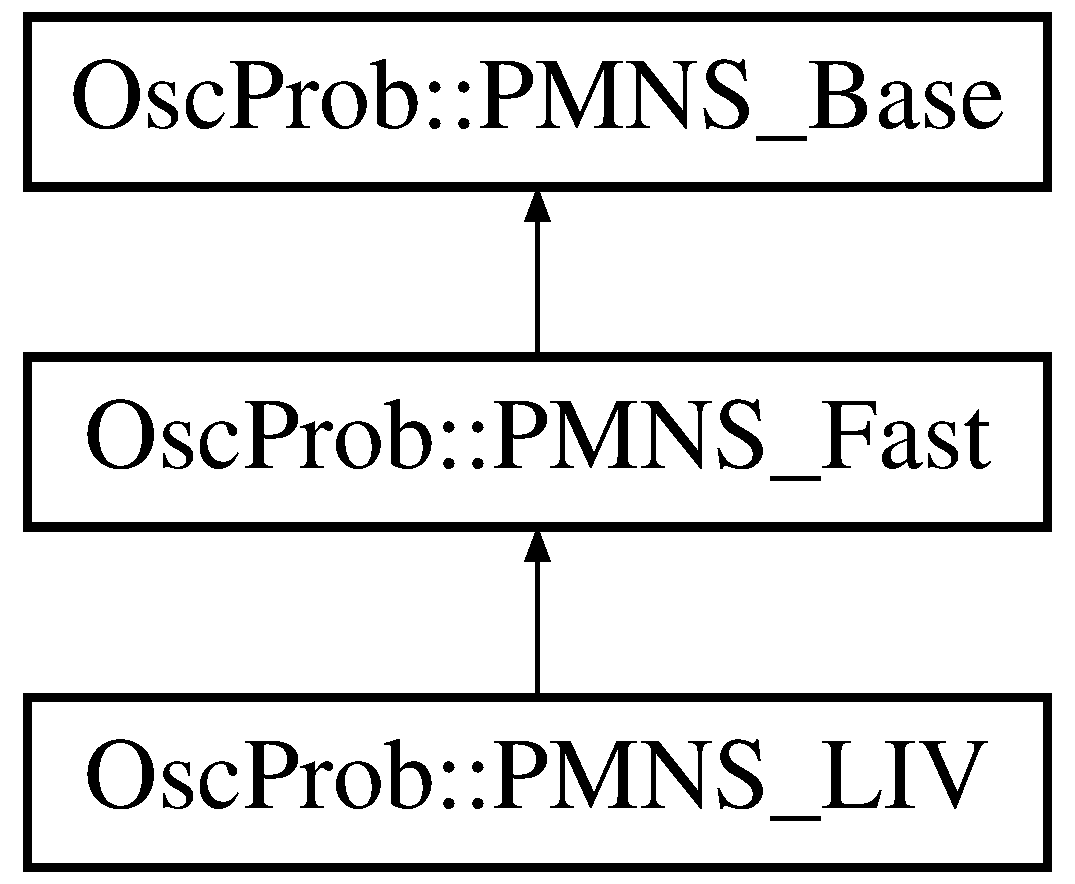
\includegraphics[height=3.000000cm]{classOscProb_1_1PMNS__LIV}
\end{center}
\end{figure}
\subsection*{Public Member Functions}
\begin{DoxyCompactItemize}
\item 
\hyperlink{classOscProb_1_1PMNS__LIV_a4a79b80700c14fe8d6a6034c6dd5870c}{P\+M\+N\+S\+\_\+\+L\+IV} ()
\begin{DoxyCompactList}\small\item\em Constructor. \end{DoxyCompactList}\item 
virtual \hyperlink{classOscProb_1_1PMNS__LIV_aa2f60af046a8c50302e67e118fc92af9}{$\sim$\+P\+M\+N\+S\+\_\+\+L\+IV} ()
\begin{DoxyCompactList}\small\item\em Destructor. \end{DoxyCompactList}\item 
virtual void \hyperlink{classOscProb_1_1PMNS__LIV_a9b21153954a8c7075c4e5826628b9608}{SetaT} (int flvi, int flvj, double val, double phase)
\begin{DoxyCompactList}\small\item\em Set any given L\+IV parameter. \end{DoxyCompactList}\item 
virtual void \hyperlink{classOscProb_1_1PMNS__LIV_aee872c8fb1e6d2bc93be711cf2455cd3}{SetcT} (int flvi, int flvj, double val, double phase)
\item 
void \hyperlink{classOscProb_1_1PMNS__LIV_a272a2e3c763ef36d08b0eacea12ea2ae}{Set\+L\+IV} (double a\+T\+\_\+ee, double a\+T\+\_\+mumu, double a\+T\+\_\+tautau, double a\+T\+\_\+emu, double a\+T\+\_\+etau, double a\+T\+\_\+mutau, double c\+T\+\_\+ee, double C\+T\+\_\+mumu, double C\+T\+\_\+tautau, double c\+T\+\_\+emu, double c\+T\+\_\+etau, double c\+T\+\_\+mutau, double delta\+\_\+a\+T\+\_\+emu=0, double delta\+\_\+a\+T\+\_\+etau=0, double delta\+\_\+a\+T\+\_\+mutau=0, double delta\+\_\+c\+T\+\_\+emu=0, double delta\+\_\+c\+T\+\_\+etau=0, double delta\+\_\+c\+T\+\_\+mutau=0)
\begin{DoxyCompactList}\small\item\em Set the L\+IV parameters all at once. \end{DoxyCompactList}\item 
virtual void \hyperlink{classOscProb_1_1PMNS__LIV_a0118e6f5e8e2e71fc846c79965cd55b5}{Seta\+T\+\_\+ee} (double a)
\begin{DoxyCompactList}\small\item\em Set eps\+\_\+ee parameter. \end{DoxyCompactList}\item 
virtual void \hyperlink{classOscProb_1_1PMNS__LIV_a9cba1afc0bb45082e6af8e8b8570e762}{Seta\+T\+\_\+mumu} (double a)
\begin{DoxyCompactList}\small\item\em Set eps\+\_\+mumu parameter. \end{DoxyCompactList}\item 
virtual void \hyperlink{classOscProb_1_1PMNS__LIV_a296ae6961e988e5919ae0b1e30706236}{Seta\+T\+\_\+tautau} (double a)
\begin{DoxyCompactList}\small\item\em Set eps\+\_\+tautau parameter. \end{DoxyCompactList}\item 
virtual void \hyperlink{classOscProb_1_1PMNS__LIV_a083dc35476bf5b9376e0ae86c9f10433}{Setc\+T\+\_\+ee} (double a)
\begin{DoxyCompactList}\small\item\em Set eps\+\_\+ee parameter. \end{DoxyCompactList}\item 
virtual void \hyperlink{classOscProb_1_1PMNS__LIV_aa09b713f8535aa74faacb01053cfc690}{Setc\+T\+\_\+mumu} (double a)
\begin{DoxyCompactList}\small\item\em Set eps\+\_\+mumu parameter. \end{DoxyCompactList}\item 
virtual void \hyperlink{classOscProb_1_1PMNS__LIV_a78e4c3cbe8fefc8766d29708316c2634}{Setc\+T\+\_\+tautau} (double a)
\begin{DoxyCompactList}\small\item\em Set eps\+\_\+tautau parameter. \end{DoxyCompactList}\item 
virtual void \hyperlink{classOscProb_1_1PMNS__LIV_a85da0e3c86280f8b0f59e03cc78caf90}{Seta\+T\+\_\+emu} (double a, double phi)
\begin{DoxyCompactList}\small\item\em Set diagonal L\+IV pars. \end{DoxyCompactList}\item 
virtual void \hyperlink{classOscProb_1_1PMNS__LIV_aee676ecf9bdc0086ade892dd534ae9ef}{Seta\+T\+\_\+etau} (double a, double phi)
\item 
virtual void \hyperlink{classOscProb_1_1PMNS__LIV_a9ea5ad11f8f7cd227230a8d83cae5419}{Seta\+T\+\_\+mutau} (double a, double phi)
\item 
virtual void \hyperlink{classOscProb_1_1PMNS__LIV_a9b3ca3e54d0195da5dd679d2624362d2}{Setc\+T\+\_\+emu} (double a, double phi)
\item 
virtual void \hyperlink{classOscProb_1_1PMNS__LIV_a588a2ede297326ce1716e91ad8d72742}{Setc\+T\+\_\+etau} (double a, double phi)
\item 
virtual void \hyperlink{classOscProb_1_1PMNS__LIV_a584ce92e7c3c55efe809842114523365}{Setc\+T\+\_\+mutau} (double a, double phi)
\item 
virtual \hyperlink{EigenPoint_8h_a67ca8e107e20610c3fff78d5e726ece0}{complexD} \hyperlink{classOscProb_1_1PMNS__LIV_a7e0c2ca289729b5736bbbccc5c15ab09}{GetaT} (int flvi, int flvj)
\begin{DoxyCompactList}\small\item\em Get any given L\+IV par. \end{DoxyCompactList}\item 
virtual \hyperlink{EigenPoint_8h_a67ca8e107e20610c3fff78d5e726ece0}{complexD} \hyperlink{classOscProb_1_1PMNS__LIV_a91b249e33e6bf12a44b7d52d96679a92}{GetcT} (int flvi, int flvj)
\item 
virtual void \hyperlink{classOscProb_1_1PMNS__Fast_ad849b2231d99c5d66fb3ade8efb896e1}{Set\+Mix} (double th12, double th23, double th13, double deltacp)
\begin{DoxyCompactList}\small\item\em Set the all mixing parameters at once. \end{DoxyCompactList}\item 
virtual void \hyperlink{classOscProb_1_1PMNS__Fast_a63733b246e6d2e609ce3de7a65ba5b9f}{Set\+Delta\+Msqrs} (double dm21, double dm32)
\begin{DoxyCompactList}\small\item\em Set both mass-\/splittings at once. \end{DoxyCompactList}\item 
virtual double \hyperlink{classOscProb_1_1PMNS__Base_aa2e10704d2d205a1ec8988de14b1a66f}{Prob} (std\+::vector$<$ \hyperlink{EigenPoint_8h_a67ca8e107e20610c3fff78d5e726ece0}{complexD} $>$ nu\+\_\+in, int flvf)
\begin{DoxyCompactList}\small\item\em Compute the probability of nu\+\_\+in going to flvf. \end{DoxyCompactList}\item 
virtual double \hyperlink{classOscProb_1_1PMNS__Base_a0190a79284289aacf682c78d7cef9a81}{Prob} (std\+::vector$<$ \hyperlink{EigenPoint_8h_a67ca8e107e20610c3fff78d5e726ece0}{complexD} $>$ nu\+\_\+in, int flvf, double E)
\begin{DoxyCompactList}\small\item\em Compute the probability of nu\+\_\+in going to flvf for energy E. \end{DoxyCompactList}\item 
virtual double \hyperlink{classOscProb_1_1PMNS__Base_a01fba31729345376705e02408e835f67}{Prob} (std\+::vector$<$ \hyperlink{EigenPoint_8h_a67ca8e107e20610c3fff78d5e726ece0}{complexD} $>$ nu\+\_\+in, int flvf, double E, double L)
\begin{DoxyCompactList}\small\item\em Compute the probability of nu\+\_\+in going to flvf for energy E and distance L. \end{DoxyCompactList}\item 
virtual double \hyperlink{classOscProb_1_1PMNS__Base_aec5c399b93261f1962a4b7dbbb44b973}{Prob} (int flvi, int flvf)
\begin{DoxyCompactList}\small\item\em Compute the probability of flvi going to flvf. \end{DoxyCompactList}\item 
virtual double \hyperlink{classOscProb_1_1PMNS__Base_aa3cee10639d5c0879ccb9e78d62128d3}{Prob} (int flvi, int flvf, double E)
\begin{DoxyCompactList}\small\item\em Compute the probability of flvi going to flvf for energy E. \end{DoxyCompactList}\item 
virtual double \hyperlink{classOscProb_1_1PMNS__Base_a6e0a74508d9d6db7be02e242b8467563}{Prob} (int flvi, int flvf, double E, double L)
\begin{DoxyCompactList}\small\item\em Compute the probability of flvi going to flvf for energy E and distance L. \end{DoxyCompactList}\item 
virtual double \hyperlink{classOscProb_1_1PMNS__Base_a89e54c80ae8a31effbab7b2b970606bb}{Avg\+Prob} (std\+::vector$<$ \hyperlink{EigenPoint_8h_a67ca8e107e20610c3fff78d5e726ece0}{complexD} $>$ nu\+\_\+in, int flvf, double E, double dE=0)
\begin{DoxyCompactList}\small\item\em Compute the average probability over a bin of energy. \end{DoxyCompactList}\item 
virtual double \hyperlink{classOscProb_1_1PMNS__Base_ac03f754160422e6600da8dbae0f803ed}{Avg\+Prob} (int flvi, int flvf, double E, double dE=0)
\begin{DoxyCompactList}\small\item\em Compute the average probability over a bin of energy. \end{DoxyCompactList}\item 
virtual double \hyperlink{classOscProb_1_1PMNS__Base_a19f160c045a01e5083506e925fb37d44}{Avg\+Prob\+LoE} (std\+::vector$<$ \hyperlink{EigenPoint_8h_a67ca8e107e20610c3fff78d5e726ece0}{complexD} $>$ nu\+\_\+in, int flvf, double LoE, double d\+LoE=0)
\begin{DoxyCompactList}\small\item\em Compute the average probability over a bin of L/E. \end{DoxyCompactList}\item 
virtual double \hyperlink{classOscProb_1_1PMNS__Base_ac19a92f4ef428a7333ca8eed76fca637}{Avg\+Prob\+LoE} (int flvi, int flvf, double LoE, double d\+LoE=0)
\begin{DoxyCompactList}\small\item\em Compute the average probability over a bin of L/E. \end{DoxyCompactList}\item 
virtual std\+::vector$<$ \hyperlink{EigenPoint_8h_a67ca8e107e20610c3fff78d5e726ece0}{complexD} $>$ \hyperlink{classOscProb_1_1PMNS__Base_a5092561dd8579d390c649eb60803ea98}{Get\+Mass\+Eigenstate} (int mi)
\begin{DoxyCompactList}\small\item\em Get a neutrino mass eigenstate. \end{DoxyCompactList}\item 
virtual void \hyperlink{classOscProb_1_1PMNS__Base_ace7875cf6d3bec161a2b7ed2690aec34}{Set\+Angle} (int i, int j, double th)
\begin{DoxyCompactList}\small\item\em Set the mixing angle theta\+\_\+ij. \end{DoxyCompactList}\item 
virtual void \hyperlink{classOscProb_1_1PMNS__Base_a4bef78cfcfc4e70b4ce79cdb8862c0a3}{Set\+Delta} (int i, int j, double delta)
\begin{DoxyCompactList}\small\item\em Set the CP phase delta\+\_\+ij. \end{DoxyCompactList}\item 
virtual void \hyperlink{classOscProb_1_1PMNS__Base_a492243b22fb1b783cd2943f507cff970}{Set\+Dm} (int j, double dm)
\begin{DoxyCompactList}\small\item\em Set the mass-\/splitting dm\+\_\+j1 in e\+V$^\wedge$2. \end{DoxyCompactList}\item 
virtual double \hyperlink{classOscProb_1_1PMNS__Base_acee137091304c919642293ddf015bbc8}{Get\+Angle} (int i, int j)
\begin{DoxyCompactList}\small\item\em Get the mixing angle theta\+\_\+ij. \end{DoxyCompactList}\item 
virtual double \hyperlink{classOscProb_1_1PMNS__Base_adb8dbc91d4286d2e7c8f768c59476241}{Get\+Delta} (int i, int j)
\begin{DoxyCompactList}\small\item\em Get the CP phase delta\+\_\+ij. \end{DoxyCompactList}\item 
virtual double \hyperlink{classOscProb_1_1PMNS__Base_ad26815ac5f4805d1259817e4936e5f8f}{Get\+Dm} (int j)
\begin{DoxyCompactList}\small\item\em Get the mass-\/splitting dm\+\_\+j1 in e\+V$^\wedge$2. \end{DoxyCompactList}\item 
virtual double \hyperlink{classOscProb_1_1PMNS__Base_a4ea861a6707ce1be3a54aad2b60f8632}{Get\+Dm\+Eff} (int j)
\begin{DoxyCompactList}\small\item\em Get the effective mass-\/splitting dm\+\_\+j1 in e\+V$^\wedge$2. \end{DoxyCompactList}\item 
virtual void \hyperlink{classOscProb_1_1PMNS__Base_a4de96ac9b6d1e9b029ab877e57d211ad}{Set\+Std\+Pars} ()
\begin{DoxyCompactList}\small\item\em Set P\+DG 3-\/flavor parameters. \end{DoxyCompactList}\item 
virtual void \hyperlink{classOscProb_1_1PMNS__Base_a95b3b0d0cab5e6a54b5ef99587f837c0}{Set\+Energy} (double E)
\begin{DoxyCompactList}\small\item\em Set the neutrino energy in GeV. \end{DoxyCompactList}\item 
virtual void \hyperlink{classOscProb_1_1PMNS__Base_a717e0348cf762f3961854e332a9b52e0}{Set\+Is\+Nu\+Bar} (bool is\+Nu\+Bar)
\begin{DoxyCompactList}\small\item\em Set the anti-\/neutrino flag. \end{DoxyCompactList}\item 
virtual double \hyperlink{classOscProb_1_1PMNS__Base_acc0d46cc4b8f911b40b807225003bbed}{Get\+Energy} ()
\begin{DoxyCompactList}\small\item\em Get the neutrino energy in GeV. \end{DoxyCompactList}\item 
virtual bool \hyperlink{classOscProb_1_1PMNS__Base_a2f7f2a028dfe7a90fff6b4f757972c2c}{Get\+Is\+Nu\+Bar} ()
\begin{DoxyCompactList}\small\item\em Get the anti-\/neutrino flag. \end{DoxyCompactList}\item 
virtual void \hyperlink{classOscProb_1_1PMNS__Base_ac3b644fd0a56347d304ceca4ae9d8875}{Set\+Path} (\hyperlink{structOscProb_1_1NuPath}{Osc\+Prob\+::\+Nu\+Path} p)
\begin{DoxyCompactList}\small\item\em Set a single path. \end{DoxyCompactList}\item 
virtual void \hyperlink{classOscProb_1_1PMNS__Base_a35b983270613072a3df58b574d80dbfd}{Set\+Path} (double length, double density, double zoa=0.\+5, int layer=0)
\begin{DoxyCompactList}\small\item\em Set a single path. \end{DoxyCompactList}\item 
virtual void \hyperlink{classOscProb_1_1PMNS__Base_a637d19dd850b4246507796526622643c}{Set\+Path} (std\+::vector$<$ \hyperlink{structOscProb_1_1NuPath}{Osc\+Prob\+::\+Nu\+Path} $>$ paths)
\begin{DoxyCompactList}\small\item\em Set a path sequence. \end{DoxyCompactList}\item 
virtual void \hyperlink{classOscProb_1_1PMNS__Base_a887dc9d4dc569ec0cdef3933b4c60efc}{Add\+Path} (\hyperlink{structOscProb_1_1NuPath}{Osc\+Prob\+::\+Nu\+Path} p)
\begin{DoxyCompactList}\small\item\em Add a path to the sequence. \end{DoxyCompactList}\item 
virtual void \hyperlink{classOscProb_1_1PMNS__Base_ab7f89ad9e7e1224adaa59d3c41594cd9}{Add\+Path} (double length, double density, double zoa=0.\+5, int layer=0)
\begin{DoxyCompactList}\small\item\em Add a path to the sequence. \end{DoxyCompactList}\item 
virtual void \hyperlink{classOscProb_1_1PMNS__Base_aefe521239031c418cfaaaa550a6e13bb}{Clear\+Path} ()
\begin{DoxyCompactList}\small\item\em Clear the path vector. \end{DoxyCompactList}\item 
virtual void \hyperlink{classOscProb_1_1PMNS__Base_a6241325b1bd28cafa556daaecbe4ed62}{Set\+Length} (double L)
\begin{DoxyCompactList}\small\item\em Set a single path lentgh in km. \end{DoxyCompactList}\item 
virtual void \hyperlink{classOscProb_1_1PMNS__Base_aa34a40a3b5abda0f252982d9ead3b520}{Set\+Length} (std\+::vector$<$ double $>$ L)
\begin{DoxyCompactList}\small\item\em Set multiple path lengths. \end{DoxyCompactList}\item 
virtual void \hyperlink{classOscProb_1_1PMNS__Base_ac74206f349687da141392c81e2ba6b0d}{Set\+Density} (double rho)
\begin{DoxyCompactList}\small\item\em Set single path density in g/cm$^\wedge$3. \end{DoxyCompactList}\item 
virtual void \hyperlink{classOscProb_1_1PMNS__Base_a858221d5510fe732dc6a101fd305cda0}{Set\+Density} (std\+::vector$<$ double $>$ rho)
\begin{DoxyCompactList}\small\item\em Set multiple path densities. \end{DoxyCompactList}\item 
virtual void \hyperlink{classOscProb_1_1PMNS__Base_a1bf3ea8fd2507fd2fd82d7410ff8f578}{Set\+ZoA} (double zoa)
\begin{DoxyCompactList}\small\item\em Set Z/A value for single path. \end{DoxyCompactList}\item 
virtual void \hyperlink{classOscProb_1_1PMNS__Base_a8495f8a320e1a21965e6a64aec92ad2a}{Set\+ZoA} (std\+::vector$<$ double $>$ zoa)
\begin{DoxyCompactList}\small\item\em Set multiple path Z/A values. \end{DoxyCompactList}\item 
virtual void \hyperlink{classOscProb_1_1PMNS__Base_a904e580edf89fb98bf9a6397739b4ebe}{Set\+Layers} (std\+::vector$<$ int $>$ lay)
\begin{DoxyCompactList}\small\item\em Set multiple path layer indices. \end{DoxyCompactList}\item 
virtual void \hyperlink{classOscProb_1_1PMNS__Base_add6533a9fc9acdfc7ae258b62570d78d}{Set\+Std\+Path} ()
\begin{DoxyCompactList}\small\item\em Set standard neutrino path. \end{DoxyCompactList}\item 
virtual std\+::vector$<$ \hyperlink{structOscProb_1_1NuPath}{Osc\+Prob\+::\+Nu\+Path} $>$ \hyperlink{classOscProb_1_1PMNS__Base_ac8e196f2e85a2b1caaf705073ee95a5c}{Get\+Path} ()
\begin{DoxyCompactList}\small\item\em Get the neutrino path sequence. \end{DoxyCompactList}\item 
virtual std\+::vector$<$ double $>$ \hyperlink{classOscProb_1_1PMNS__Base_a9eac8d768c1424755ee41f7e783af179}{Get\+Sample\+Points} (double LoE, double d\+LoE)
\begin{DoxyCompactList}\small\item\em Compute the sample points for a bin of L/E with width d\+LoE. \end{DoxyCompactList}\item 
virtual void \hyperlink{classOscProb_1_1PMNS__Base_aa94c1e1fff0ba731c75f7e633b023a9f}{Set\+Use\+Cache} (bool u=true)
\begin{DoxyCompactList}\small\item\em Set caching on/off. \end{DoxyCompactList}\item 
virtual void \hyperlink{classOscProb_1_1PMNS__Base_ac47fd33e69aa6490f99e2fd147a92f03}{Clear\+Cache} ()
\begin{DoxyCompactList}\small\item\em Clear the cache. \end{DoxyCompactList}\item 
virtual void \hyperlink{classOscProb_1_1PMNS__Base_ae67862cf58b0802487a14b047b012a78}{Set\+Max\+Cache} (int mc=1e6)
\begin{DoxyCompactList}\small\item\em Set max cache size. \end{DoxyCompactList}\end{DoxyCompactItemize}
\subsection*{Protected Member Functions}
\begin{DoxyCompactItemize}
\item 
virtual void \hyperlink{classOscProb_1_1PMNS__LIV_a848fc59ce966126dc6d6e6c32621ad6c}{Update\+Ham} ()
\begin{DoxyCompactList}\small\item\em Build the full Hamiltonian. \end{DoxyCompactList}\item 
virtual void \hyperlink{classOscProb_1_1PMNS__Fast_a8a0828401591e88c60e0051fbfe02d5e}{Solve\+Ham} ()
\begin{DoxyCompactList}\small\item\em Solve the full Hamiltonian for eigenvectors and eigenvalues. \end{DoxyCompactList}\item 
virtual void \hyperlink{classOscProb_1_1PMNS__Fast_a76dd5a761df8689c502b28ad0391f9e2}{Set\+Vacuum\+Eigensystem} ()
\begin{DoxyCompactList}\small\item\em Set the eigensystem to the analytic solution of the vacuum Hamiltonian. \end{DoxyCompactList}\item 
virtual void \hyperlink{classOscProb_1_1PMNS__Base_adf23b569112f9f9e0e592f01d79a5f3d}{Initialize\+Vectors} ()
\begin{DoxyCompactList}\small\item\em Initialize all member vectors with zeros. \end{DoxyCompactList}\item 
virtual bool \hyperlink{classOscProb_1_1PMNS__Base_abe533da5f64bec1f4724ab7b58606b77}{Try\+Cache} ()
\begin{DoxyCompactList}\small\item\em Try to find a cached eigensystem. \end{DoxyCompactList}\item 
virtual void \hyperlink{classOscProb_1_1PMNS__Base_a785c37fcea974628623c8881bb0fbbf9}{Fill\+Cache} ()
\begin{DoxyCompactList}\small\item\em Cache the current eigensystem. \end{DoxyCompactList}\item 
virtual void \hyperlink{classOscProb_1_1PMNS__Base_a986e6ebef09a7e2eb7fee16a4c2c834d}{Set\+Cur\+Path} (\hyperlink{structOscProb_1_1NuPath}{Osc\+Prob\+::\+Nu\+Path} p)
\begin{DoxyCompactList}\small\item\em Set the path currently in use by the class. \end{DoxyCompactList}\item 
virtual void \hyperlink{classOscProb_1_1PMNS__Base_aba565962a440d14bee7a2a96d2eca2c5}{Set\+Att} (double att, int idx)
\begin{DoxyCompactList}\small\item\em Set one of the path attributes. \end{DoxyCompactList}\item 
virtual void \hyperlink{classOscProb_1_1PMNS__Base_aa001479b5f5828c3d16ed087f96ecbcc}{Set\+Att} (std\+::vector$<$ double $>$ att, int idx)
\begin{DoxyCompactList}\small\item\em Set all values of a path attribute. \end{DoxyCompactList}\item 
virtual void \hyperlink{classOscProb_1_1PMNS__Base_a6a3cf45bbe2349abf06708b65677c044}{RotateH} (int i, int j, std\+::vector$<$ std\+::vector$<$ \hyperlink{EigenPoint_8h_a67ca8e107e20610c3fff78d5e726ece0}{complexD} $>$ $>$ \&Ham)
\begin{DoxyCompactList}\small\item\em Rotate the Hamiltonian by theta\+\_\+ij and delta\+\_\+ij. \end{DoxyCompactList}\item 
virtual void \hyperlink{classOscProb_1_1PMNS__Base_ae52554477ad3250daa5adb8c32cab0b4}{Rotate\+State} (int i, int j)
\begin{DoxyCompactList}\small\item\em Rotate the neutrino state by theta\+\_\+ij and delta\+\_\+ij. \end{DoxyCompactList}\item 
virtual void \hyperlink{classOscProb_1_1PMNS__Base_ad0faf5eae755afb1baa1fcd5ffebad41}{Build\+Hms} ()
\begin{DoxyCompactList}\small\item\em Build the matrix of masses squared. \end{DoxyCompactList}\item 
virtual void \hyperlink{classOscProb_1_1PMNS__Base_ac0d4bf8ff1318ef96d3dafa62e0cec25}{Reset\+To\+Flavour} (int flv)
\begin{DoxyCompactList}\small\item\em Reset neutrino state to pure flavour flv. \end{DoxyCompactList}\item 
virtual void \hyperlink{classOscProb_1_1PMNS__Base_accb08503acc162188041d7a96a280462}{Propagate\+Path} (\hyperlink{structOscProb_1_1NuPath}{Osc\+Prob\+::\+Nu\+Path} p)
\begin{DoxyCompactList}\small\item\em Propagate neutrino through a single path. \end{DoxyCompactList}\item 
virtual void \hyperlink{classOscProb_1_1PMNS__Base_a054e3a8b05b9a958b6fa416e4a835e3e}{Propagate} ()
\begin{DoxyCompactList}\small\item\em Propagate neutrino through full path. \end{DoxyCompactList}\item 
virtual double \hyperlink{classOscProb_1_1PMNS__Base_a0dc4d45bc3d7e03b9abbf5b4e100cc22}{P} (int flv)
\begin{DoxyCompactList}\small\item\em Return the probability of final state in flavour flv. \end{DoxyCompactList}\end{DoxyCompactItemize}
\subsection*{Protected Attributes}
\begin{DoxyCompactItemize}
\item 
\hyperlink{EigenPoint_8h_a67ca8e107e20610c3fff78d5e726ece0}{complexD} \hyperlink{classOscProb_1_1PMNS__LIV_ae6b7440e4bae5b2783e7c6e7d03d816b}{faT} \mbox{[}3\mbox{]}\mbox{[}3\mbox{]}
\begin{DoxyCompactList}\small\item\em Stores each L\+I\+V1 parameter. \end{DoxyCompactList}\item 
\hyperlink{EigenPoint_8h_a67ca8e107e20610c3fff78d5e726ece0}{complexD} \hyperlink{classOscProb_1_1PMNS__LIV_aa029c6be1133f8efa17524822b49d619}{fcT} \mbox{[}3\mbox{]}\mbox{[}3\mbox{]}
\begin{DoxyCompactList}\small\item\em Stores each L\+I\+V1 parameter. \end{DoxyCompactList}\item 
\hyperlink{EigenPoint_8h_a67ca8e107e20610c3fff78d5e726ece0}{complexD} \hyperlink{classOscProb_1_1PMNS__Fast_a94286a881bc53dd512a89d548346b611}{f\+Ham} \mbox{[}3\mbox{]}\mbox{[}3\mbox{]}
\begin{DoxyCompactList}\small\item\em The full hamiltonian. \end{DoxyCompactList}\item 
int \hyperlink{classOscProb_1_1PMNS__Base_a24bb74bed63569dfe88b18fa6a08060e}{f\+Num\+Nus}
\begin{DoxyCompactList}\small\item\em Number of neutrino flavours. \end{DoxyCompactList}\item 
std\+::vector$<$ double $>$ \hyperlink{classOscProb_1_1PMNS__Base_a406a31c3b5d620e5a0cace5b411f9f70}{f\+Dm}
\begin{DoxyCompactList}\small\item\em m$^\wedge$2\+\_\+i -\/ m$^\wedge$2\+\_\+1 in vacuum \end{DoxyCompactList}\item 
std\+::vector$<$ std\+::vector$<$ double $>$ $>$ \hyperlink{classOscProb_1_1PMNS__Base_a1976887cd658dd86b2336c181f1470b4}{f\+Theta}
\begin{DoxyCompactList}\small\item\em theta\mbox{[}i\mbox{]}\mbox{[}j\mbox{]} mixing angle \end{DoxyCompactList}\item 
std\+::vector$<$ std\+::vector$<$ double $>$ $>$ \hyperlink{classOscProb_1_1PMNS__Base_ab2a5fa40e689b221c8a7d2c17213810d}{f\+Delta}
\begin{DoxyCompactList}\small\item\em delta\mbox{[}i\mbox{]}\mbox{[}j\mbox{]} CP violating phase \end{DoxyCompactList}\item 
std\+::vector$<$ \hyperlink{EigenPoint_8h_a67ca8e107e20610c3fff78d5e726ece0}{complexD} $>$ \hyperlink{classOscProb_1_1PMNS__Base_abf99f2339e3ee989600740b5d88063e8}{f\+Nu\+State}
\begin{DoxyCompactList}\small\item\em The neutrino current state. \end{DoxyCompactList}\item 
std\+::vector$<$ std\+::vector$<$ \hyperlink{EigenPoint_8h_a67ca8e107e20610c3fff78d5e726ece0}{complexD} $>$ $>$ \hyperlink{classOscProb_1_1PMNS__Base_acd3c8783e7603081eab316ea4c86c766}{f\+Hms}
\begin{DoxyCompactList}\small\item\em matrix H$\ast$2E in e\+V$^\wedge$2 \end{DoxyCompactList}\item 
std\+::vector$<$ \hyperlink{EigenPoint_8h_a67ca8e107e20610c3fff78d5e726ece0}{complexD} $>$ \hyperlink{classOscProb_1_1PMNS__Base_ab8d26b722047d49d977f5f2d83026ede}{f\+Phases}
\begin{DoxyCompactList}\small\item\em Buffer for oscillation phases. \end{DoxyCompactList}\item 
std\+::vector$<$ \hyperlink{EigenPoint_8h_a67ca8e107e20610c3fff78d5e726ece0}{complexD} $>$ \hyperlink{classOscProb_1_1PMNS__Base_a5440bc3efa466a37649601abce559e3e}{f\+Buffer}
\begin{DoxyCompactList}\small\item\em Buffer for neutrino state tranformations. \end{DoxyCompactList}\item 
std\+::vector$<$ double $>$ \hyperlink{classOscProb_1_1PMNS__Base_a6319c34d7decbb9d7d6da279c06e8c2d}{f\+Eval}
\begin{DoxyCompactList}\small\item\em Eigenvalues of the Hamiltonian. \end{DoxyCompactList}\item 
std\+::vector$<$ std\+::vector$<$ \hyperlink{EigenPoint_8h_a67ca8e107e20610c3fff78d5e726ece0}{complexD} $>$ $>$ \hyperlink{classOscProb_1_1PMNS__Base_a87be137356c5f27ab83cab5e1298ef8f}{f\+Evec}
\begin{DoxyCompactList}\small\item\em Eigenvectors of the Hamiltonian. \end{DoxyCompactList}\item 
double \hyperlink{classOscProb_1_1PMNS__Base_a2800af6d436972f3e900867790c046b0}{f\+Energy}
\begin{DoxyCompactList}\small\item\em Neutrino energy. \end{DoxyCompactList}\item 
bool \hyperlink{classOscProb_1_1PMNS__Base_a0ebaeaefab36a3ff381c6293faedfdd6}{f\+Is\+Nu\+Bar}
\begin{DoxyCompactList}\small\item\em Anti-\/neutrino flag. \end{DoxyCompactList}\item 
std\+::vector$<$ \hyperlink{structOscProb_1_1NuPath}{Osc\+Prob\+::\+Nu\+Path} $>$ \hyperlink{classOscProb_1_1PMNS__Base_a69db9d57e12fc7cbe0431bc6c18fac93}{f\+Nu\+Paths}
\begin{DoxyCompactList}\small\item\em Vector of neutrino paths. \end{DoxyCompactList}\item 
\hyperlink{structOscProb_1_1NuPath}{Osc\+Prob\+::\+Nu\+Path} \hyperlink{classOscProb_1_1PMNS__Base_a849437aa8891fe042e86886ce8f81c6e}{f\+Path}
\begin{DoxyCompactList}\small\item\em Current neutrino path. \end{DoxyCompactList}\item 
bool \hyperlink{classOscProb_1_1PMNS__Base_a9ac3cadeac8db1b90f3152f476244780}{f\+Built\+Hms}
\begin{DoxyCompactList}\small\item\em Tag to avoid rebuilding Hms. \end{DoxyCompactList}\item 
bool \hyperlink{classOscProb_1_1PMNS__Base_a6dc5cd010d2d70b2324745b4e53e9839}{f\+Got\+ES}
\begin{DoxyCompactList}\small\item\em Tag to avoid recalculating eigensystem. \end{DoxyCompactList}\item 
bool \hyperlink{classOscProb_1_1PMNS__Base_ad28c12ef897b5555eda509ea55c99107}{f\+Use\+Cache}
\begin{DoxyCompactList}\small\item\em Flag for whether to use caching. \end{DoxyCompactList}\item 
double \hyperlink{classOscProb_1_1PMNS__Base_a0b4c41a27de281472453a1912cbc1e64}{f\+Cache\+Prec}
\begin{DoxyCompactList}\small\item\em Precision of cache matching. \end{DoxyCompactList}\item 
int \hyperlink{classOscProb_1_1PMNS__Base_a74c13356eafec2490d8c3c19759ba7f0}{f\+Max\+Cache}
\begin{DoxyCompactList}\small\item\em Maximum cache size. \end{DoxyCompactList}\item 
std\+::set$<$ \hyperlink{structOscProb_1_1EigenPoint}{Osc\+Prob\+::\+Eigen\+Point} $>$ \hyperlink{classOscProb_1_1PMNS__Base_a8159424f20197a3a7145fe3bf2c11176}{f\+Mix\+Cache}
\begin{DoxyCompactList}\small\item\em Caching set of eigensystems. \end{DoxyCompactList}\item 
\hyperlink{structOscProb_1_1EigenPoint}{Eigen\+Point} \hyperlink{classOscProb_1_1PMNS__Base_ab1fe4800ee3ae48df4fc942dce00e0d3}{f\+Probe}
\begin{DoxyCompactList}\small\item\em Eigenp\+Point to try. \end{DoxyCompactList}\end{DoxyCompactItemize}
\subsection*{Static Protected Attributes}
\begin{DoxyCompactItemize}
\item 
static const \hyperlink{EigenPoint_8h_a67ca8e107e20610c3fff78d5e726ece0}{complexD} \hyperlink{classOscProb_1_1PMNS__Base_a05e595848c2521dc795efa7645728b94}{zero}
\begin{DoxyCompactList}\small\item\em zero in complex \end{DoxyCompactList}\item 
static const \hyperlink{EigenPoint_8h_a67ca8e107e20610c3fff78d5e726ece0}{complexD} \hyperlink{classOscProb_1_1PMNS__Base_a7d1d0bbcab30a1fd8c368c40134c51ff}{one}
\begin{DoxyCompactList}\small\item\em one in complex \end{DoxyCompactList}\item 
static const double \hyperlink{classOscProb_1_1PMNS__Base_a382ddd7b76ca89b43f22614a2ea7327b}{k\+Km2eV} = 1.\+0 / 1.\+973269788e-\/10
\begin{DoxyCompactList}\small\item\em km to e\+V$^\wedge$-\/1 \end{DoxyCompactList}\item 
static const double \hyperlink{classOscProb_1_1PMNS__Base_a326fc5016d7dd7ce05682c06cdcb6d94}{k\+K2} = 1e-\/3 $\ast$ k\+N\+A / pow(k\+Km2e\+V,3)
\begin{DoxyCompactList}\small\item\em mol/\+Ge\+V$^\wedge$2/cm$^\wedge$3 to eV \end{DoxyCompactList}\item 
static const double \hyperlink{classOscProb_1_1PMNS__Base_ad36a0a6bf58d6ec093d3947784bd89e9}{k\+Ge\+V2eV} = 1.\+0e+09
\begin{DoxyCompactList}\small\item\em GeV to eV. \end{DoxyCompactList}\item 
static const double \hyperlink{classOscProb_1_1PMNS__Base_a69355e770b89e99437c2b8a66e48eeb9}{k\+NA} = 6.\+022140857e23
\begin{DoxyCompactList}\small\item\em Avogadro constant. \end{DoxyCompactList}\item 
static const double \hyperlink{classOscProb_1_1PMNS__Base_a7f26a3456128234b2ae6cc9141a6532f}{k\+Gf} = 1.\+1663787e-\/05
\begin{DoxyCompactList}\small\item\em G\+\_\+F in units of Ge\+V$^\wedge$-\/2. \end{DoxyCompactList}\end{DoxyCompactItemize}


\subsection{Detailed Description}


Definition at line 17 of file P\+M\+N\+S\+\_\+\+L\+I\+V.\+h.



\subsection{Constructor \& Destructor Documentation}
\mbox{\Hypertarget{classOscProb_1_1PMNS__LIV_a4a79b80700c14fe8d6a6034c6dd5870c}\label{classOscProb_1_1PMNS__LIV_a4a79b80700c14fe8d6a6034c6dd5870c}} 
\index{Osc\+Prob\+::\+P\+M\+N\+S\+\_\+\+L\+IV@{Osc\+Prob\+::\+P\+M\+N\+S\+\_\+\+L\+IV}!P\+M\+N\+S\+\_\+\+L\+IV@{P\+M\+N\+S\+\_\+\+L\+IV}}
\index{P\+M\+N\+S\+\_\+\+L\+IV@{P\+M\+N\+S\+\_\+\+L\+IV}!Osc\+Prob\+::\+P\+M\+N\+S\+\_\+\+L\+IV@{Osc\+Prob\+::\+P\+M\+N\+S\+\_\+\+L\+IV}}
\subsubsection{\texorpdfstring{P\+M\+N\+S\+\_\+\+L\+I\+V()}{PMNS\_LIV()}}
{\footnotesize\ttfamily P\+M\+N\+S\+\_\+\+L\+I\+V\+::\+P\+M\+N\+S\+\_\+\+L\+IV (\begin{DoxyParamCaption}{ }\end{DoxyParamCaption})}

Constructor. \begin{DoxySeeAlso}{See also}
\hyperlink{classOscProb_1_1PMNS__Base_aa53e83b03a9cf4bdfa0a07136bd17a79}{P\+M\+N\+S\+\_\+\+Base\+::\+P\+M\+N\+S\+\_\+\+Base}
\end{DoxySeeAlso}
This class is restricted to 3 neutrino flavours. 

Definition at line 31 of file P\+M\+N\+S\+\_\+\+L\+I\+V.\+cxx.



References Set\+L\+I\+V(), and Osc\+Prob\+::\+P\+M\+N\+S\+\_\+\+Base\+::\+Set\+Std\+Path().


\begin{DoxyCode}
31                    : \hyperlink{classOscProb_1_1PMNS__Fast_a2bbac744bf63753105d766a860af7c0d}{PMNS\_Fast}()
32 \{
33   \hyperlink{classOscProb_1_1PMNS__Base_add6533a9fc9acdfc7ae258b62570d78d}{SetStdPath}();
34   \hyperlink{classOscProb_1_1PMNS__LIV_a272a2e3c763ef36d08b0eacea12ea2ae}{SetLIV}(0.,0.,0.,0.,0.,0.,0.,0.,0.,0.,0.,0.,0.,0.,0.,0.,0.,0.);
35 \}
\end{DoxyCode}
\mbox{\Hypertarget{classOscProb_1_1PMNS__LIV_aa2f60af046a8c50302e67e118fc92af9}\label{classOscProb_1_1PMNS__LIV_aa2f60af046a8c50302e67e118fc92af9}} 
\index{Osc\+Prob\+::\+P\+M\+N\+S\+\_\+\+L\+IV@{Osc\+Prob\+::\+P\+M\+N\+S\+\_\+\+L\+IV}!````~P\+M\+N\+S\+\_\+\+L\+IV@{$\sim$\+P\+M\+N\+S\+\_\+\+L\+IV}}
\index{````~P\+M\+N\+S\+\_\+\+L\+IV@{$\sim$\+P\+M\+N\+S\+\_\+\+L\+IV}!Osc\+Prob\+::\+P\+M\+N\+S\+\_\+\+L\+IV@{Osc\+Prob\+::\+P\+M\+N\+S\+\_\+\+L\+IV}}
\subsubsection{\texorpdfstring{$\sim$\+P\+M\+N\+S\+\_\+\+L\+I\+V()}{~PMNS\_LIV()}}
{\footnotesize\ttfamily P\+M\+N\+S\+\_\+\+L\+I\+V\+::$\sim$\+P\+M\+N\+S\+\_\+\+L\+IV (\begin{DoxyParamCaption}{ }\end{DoxyParamCaption})\hspace{0.3cm}{\ttfamily [virtual]}}

Nothing to clean. 

Definition at line 41 of file P\+M\+N\+S\+\_\+\+L\+I\+V.\+cxx.


\begin{DoxyCode}
41 \{\}
\end{DoxyCode}


\subsection{Member Function Documentation}
\mbox{\Hypertarget{classOscProb_1_1PMNS__Base_a887dc9d4dc569ec0cdef3933b4c60efc}\label{classOscProb_1_1PMNS__Base_a887dc9d4dc569ec0cdef3933b4c60efc}} 
\index{Osc\+Prob\+::\+P\+M\+N\+S\+\_\+\+L\+IV@{Osc\+Prob\+::\+P\+M\+N\+S\+\_\+\+L\+IV}!Add\+Path@{Add\+Path}}
\index{Add\+Path@{Add\+Path}!Osc\+Prob\+::\+P\+M\+N\+S\+\_\+\+L\+IV@{Osc\+Prob\+::\+P\+M\+N\+S\+\_\+\+L\+IV}}
\subsubsection{\texorpdfstring{Add\+Path()}{AddPath()}\hspace{0.1cm}{\footnotesize\ttfamily [1/2]}}
{\footnotesize\ttfamily void P\+M\+N\+S\+\_\+\+Base\+::\+Add\+Path (\begin{DoxyParamCaption}\item[{\hyperlink{structOscProb_1_1NuPath}{Osc\+Prob\+::\+Nu\+Path}}]{p }\end{DoxyParamCaption})\hspace{0.3cm}{\ttfamily [virtual]}, {\ttfamily [inherited]}}

Add a path to the sequence. 
\begin{DoxyParams}{Parameters}
{\em p} & -\/ A neutrino path segment \\
\hline
\end{DoxyParams}


Definition at line 351 of file P\+M\+N\+S\+\_\+\+Base.\+cxx.



References Osc\+Prob\+::\+P\+M\+N\+S\+\_\+\+Base\+::f\+Nu\+Paths.



Referenced by Osc\+Prob\+::\+P\+M\+N\+S\+\_\+\+Base\+::\+Add\+Path(), Osc\+Prob\+::\+P\+M\+N\+S\+\_\+\+Base\+::\+Set\+Att(), and Osc\+Prob\+::\+P\+M\+N\+S\+\_\+\+Base\+::\+Set\+Path().


\begin{DoxyCode}
351                                \{
352 
353   \hyperlink{classOscProb_1_1PMNS__Base_a69db9d57e12fc7cbe0431bc6c18fac93}{fNuPaths}.push\_back(p);
354 
355 \}
\end{DoxyCode}
\mbox{\Hypertarget{classOscProb_1_1PMNS__Base_ab7f89ad9e7e1224adaa59d3c41594cd9}\label{classOscProb_1_1PMNS__Base_ab7f89ad9e7e1224adaa59d3c41594cd9}} 
\index{Osc\+Prob\+::\+P\+M\+N\+S\+\_\+\+L\+IV@{Osc\+Prob\+::\+P\+M\+N\+S\+\_\+\+L\+IV}!Add\+Path@{Add\+Path}}
\index{Add\+Path@{Add\+Path}!Osc\+Prob\+::\+P\+M\+N\+S\+\_\+\+L\+IV@{Osc\+Prob\+::\+P\+M\+N\+S\+\_\+\+L\+IV}}
\subsubsection{\texorpdfstring{Add\+Path()}{AddPath()}\hspace{0.1cm}{\footnotesize\ttfamily [2/2]}}
{\footnotesize\ttfamily void P\+M\+N\+S\+\_\+\+Base\+::\+Add\+Path (\begin{DoxyParamCaption}\item[{double}]{length,  }\item[{double}]{density,  }\item[{double}]{zoa = {\ttfamily 0.5},  }\item[{int}]{layer = {\ttfamily 0} }\end{DoxyParamCaption})\hspace{0.3cm}{\ttfamily [virtual]}, {\ttfamily [inherited]}}

Add a path to the sequence defining attributes directly. 
\begin{DoxyParams}{Parameters}
{\em length} & -\/ The length of the path segment in km \\
\hline
{\em density} & -\/ The density of the path segment in g/cm$^\wedge$3 \\
\hline
{\em zoa} & -\/ The effective Z/A of the path segment \\
\hline
{\em layer} & -\/ An index to identify the layer type (e.\+g. earth inner core) \\
\hline
\end{DoxyParams}


Definition at line 365 of file P\+M\+N\+S\+\_\+\+Base.\+cxx.



References Osc\+Prob\+::\+P\+M\+N\+S\+\_\+\+Base\+::\+Add\+Path().


\begin{DoxyCode}
365                                                                            \{
366 
367   \hyperlink{classOscProb_1_1PMNS__Base_a887dc9d4dc569ec0cdef3933b4c60efc}{AddPath}(\hyperlink{structOscProb_1_1NuPath}{NuPath}(length, density, zoa, layer));
368 
369 \}
\end{DoxyCode}
\mbox{\Hypertarget{classOscProb_1_1PMNS__Base_a89e54c80ae8a31effbab7b2b970606bb}\label{classOscProb_1_1PMNS__Base_a89e54c80ae8a31effbab7b2b970606bb}} 
\index{Osc\+Prob\+::\+P\+M\+N\+S\+\_\+\+L\+IV@{Osc\+Prob\+::\+P\+M\+N\+S\+\_\+\+L\+IV}!Avg\+Prob@{Avg\+Prob}}
\index{Avg\+Prob@{Avg\+Prob}!Osc\+Prob\+::\+P\+M\+N\+S\+\_\+\+L\+IV@{Osc\+Prob\+::\+P\+M\+N\+S\+\_\+\+L\+IV}}
\subsubsection{\texorpdfstring{Avg\+Prob()}{AvgProb()}\hspace{0.1cm}{\footnotesize\ttfamily [1/2]}}
{\footnotesize\ttfamily double P\+M\+N\+S\+\_\+\+Base\+::\+Avg\+Prob (\begin{DoxyParamCaption}\item[{std\+::vector$<$ \hyperlink{EigenPoint_8h_a67ca8e107e20610c3fff78d5e726ece0}{complexD} $>$}]{nu\+\_\+in,  }\item[{int}]{flvf,  }\item[{double}]{E,  }\item[{double}]{dE = {\ttfamily 0} }\end{DoxyParamCaption})\hspace{0.3cm}{\ttfamily [virtual]}, {\ttfamily [inherited]}}

Compute the average probability of nu\+\_\+in going to flvf over a bin of energy E with width dE.

This gets transformed into L/E, since the oscillation terms have arguments linear in L/E and not E.

This function works best for single paths. In multiple paths the accuracy may be somewhat worse. If needed, average over smaller energy ranges.

Flavours are\+: 
\begin{DoxyPre}
  0 = nue, 1 = numu, 2 = nutau
  3 = sterile\_1, 4 = sterile\_2, etc.
\end{DoxyPre}
 
\begin{DoxyParams}{Parameters}
{\em nu\+\_\+in} & -\/ The neutrino initial state in flavour. \\
\hline
{\em flvf} & -\/ The neutrino final flavour. \\
\hline
{\em E} & -\/ The neutrino energy in the bin center in GeV \\
\hline
{\em dE} & -\/ The energy bin width in GeV\\
\hline
\end{DoxyParams}
\begin{DoxyReturn}{Returns}
Average neutrino oscillation probability 
\end{DoxyReturn}


Definition at line 1386 of file P\+M\+N\+S\+\_\+\+Base.\+cxx.



References Osc\+Prob\+::\+Avg\+Path(), Osc\+Prob\+::\+P\+M\+N\+S\+\_\+\+Base\+::\+Avg\+Prob\+Lo\+E(), Osc\+Prob\+::\+P\+M\+N\+S\+\_\+\+Base\+::f\+Nu\+Paths, Osc\+Prob\+::\+P\+M\+N\+S\+\_\+\+Base\+::f\+Path, Osc\+Prob\+::\+Nu\+Path\+::length, Osc\+Prob\+::\+P\+M\+N\+S\+\_\+\+Base\+::\+Prob(), and Osc\+Prob\+::\+P\+M\+N\+S\+\_\+\+Base\+::\+Set\+Cur\+Path().



Referenced by Osc\+Prob\+::\+P\+M\+N\+S\+\_\+\+Base\+::\+Avg\+Prob().


\begin{DoxyCode}
1387 \{
1388 
1389   \textcolor{comment}{// Do nothing if energy is not positive}
1390   \textcolor{keywordflow}{if}(E<=0) \textcolor{keywordflow}{return} 0;
1391 
1392   \textcolor{keywordflow}{if}(\hyperlink{classOscProb_1_1PMNS__Base_a69db9d57e12fc7cbe0431bc6c18fac93}{fNuPaths}.empty()) \textcolor{keywordflow}{return} 0;
1393 
1394   \textcolor{comment}{// Don't average zero width}
1395   \textcolor{keywordflow}{if}(dE<=0) \textcolor{keywordflow}{return} \hyperlink{classOscProb_1_1PMNS__Base_aa2e10704d2d205a1ec8988de14b1a66f}{Prob}(nu\_in, flvf, E);
1396 
1397   \textcolor{comment}{// Make sure fPath is set}
1398   \textcolor{comment}{// Use average if multiple paths}
1399   \hyperlink{classOscProb_1_1PMNS__Base_a986e6ebef09a7e2eb7fee16a4c2c834d}{SetCurPath}(\hyperlink{namespaceOscProb_a999a7944bad8bc72d7ee9f56f81a210e}{AvgPath}(\hyperlink{classOscProb_1_1PMNS__Base_a69db9d57e12fc7cbe0431bc6c18fac93}{fNuPaths}));
1400 
1401   \textcolor{comment}{// Define L/E variables}
1402   \textcolor{keywordtype}{double} LoE = 0;
1403   \textcolor{keywordtype}{double} dLoE = 0;
1404 
1405   \textcolor{comment}{// Set a minimum energy}
1406   \textcolor{keywordtype}{double} minE = 0.1 * E;
1407 
1408   \textcolor{comment}{// Transform range to L/E}
1409   \textcolor{comment}{// Full range if low edge > minE}
1410   \textcolor{keywordflow}{if}(E-dE/2 > minE)\{
1411     LoE = 0.5 * (\hyperlink{classOscProb_1_1PMNS__Base_a849437aa8891fe042e86886ce8f81c6e}{fPath}.\hyperlink{structOscProb_1_1NuPath_af22660894b6e25cf835500381b155557}{length}/(E-dE/2) + \hyperlink{classOscProb_1_1PMNS__Base_a849437aa8891fe042e86886ce8f81c6e}{fPath}.\hyperlink{structOscProb_1_1NuPath_af22660894b6e25cf835500381b155557}{length}/(E+dE/2));
1412     dLoE = \hyperlink{classOscProb_1_1PMNS__Base_a849437aa8891fe042e86886ce8f81c6e}{fPath}.\hyperlink{structOscProb_1_1NuPath_af22660894b6e25cf835500381b155557}{length}/(E-dE/2) - \hyperlink{classOscProb_1_1PMNS__Base_a849437aa8891fe042e86886ce8f81c6e}{fPath}.\hyperlink{structOscProb_1_1NuPath_af22660894b6e25cf835500381b155557}{length}/(E+dE/2);
1413   \}
1414   \textcolor{comment}{// Else start at minE}
1415   \textcolor{keywordflow}{else}\{
1416     LoE = 0.5 * (\hyperlink{classOscProb_1_1PMNS__Base_a849437aa8891fe042e86886ce8f81c6e}{fPath}.\hyperlink{structOscProb_1_1NuPath_af22660894b6e25cf835500381b155557}{length}/minE + \hyperlink{classOscProb_1_1PMNS__Base_a849437aa8891fe042e86886ce8f81c6e}{fPath}.\hyperlink{structOscProb_1_1NuPath_af22660894b6e25cf835500381b155557}{length}/(E+dE/2));
1417     dLoE = \hyperlink{classOscProb_1_1PMNS__Base_a849437aa8891fe042e86886ce8f81c6e}{fPath}.\hyperlink{structOscProb_1_1NuPath_af22660894b6e25cf835500381b155557}{length}/minE - \hyperlink{classOscProb_1_1PMNS__Base_a849437aa8891fe042e86886ce8f81c6e}{fPath}.\hyperlink{structOscProb_1_1NuPath_af22660894b6e25cf835500381b155557}{length}/(E+dE/2);
1418   \}
1419 
1420   \textcolor{comment}{// Compute average in LoE}
1421   \textcolor{keywordflow}{return} \hyperlink{classOscProb_1_1PMNS__Base_a19f160c045a01e5083506e925fb37d44}{AvgProbLoE}(nu\_in, flvf, LoE, dLoE);
1422 
1423 \}
\end{DoxyCode}
\mbox{\Hypertarget{classOscProb_1_1PMNS__Base_ac03f754160422e6600da8dbae0f803ed}\label{classOscProb_1_1PMNS__Base_ac03f754160422e6600da8dbae0f803ed}} 
\index{Osc\+Prob\+::\+P\+M\+N\+S\+\_\+\+L\+IV@{Osc\+Prob\+::\+P\+M\+N\+S\+\_\+\+L\+IV}!Avg\+Prob@{Avg\+Prob}}
\index{Avg\+Prob@{Avg\+Prob}!Osc\+Prob\+::\+P\+M\+N\+S\+\_\+\+L\+IV@{Osc\+Prob\+::\+P\+M\+N\+S\+\_\+\+L\+IV}}
\subsubsection{\texorpdfstring{Avg\+Prob()}{AvgProb()}\hspace{0.1cm}{\footnotesize\ttfamily [2/2]}}
{\footnotesize\ttfamily double P\+M\+N\+S\+\_\+\+Base\+::\+Avg\+Prob (\begin{DoxyParamCaption}\item[{int}]{flvi,  }\item[{int}]{flvf,  }\item[{double}]{E,  }\item[{double}]{dE = {\ttfamily 0} }\end{DoxyParamCaption})\hspace{0.3cm}{\ttfamily [virtual]}, {\ttfamily [inherited]}}

Compute the average probability of flvi going to flvf over a bin of energy E with width dE.

This gets transformed into L/E, since the oscillation terms have arguments linear in L/E and not E.

This function works best for single paths. In multiple paths the accuracy may be somewhat worse. If needed, average over smaller energy ranges.

Flavours are\+: 
\begin{DoxyPre}
  0 = nue, 1 = numu, 2 = nutau
  3 = sterile\_1, 4 = sterile\_2, etc.
\end{DoxyPre}
 
\begin{DoxyParams}{Parameters}
{\em flvi} & -\/ The neutrino starting flavour. \\
\hline
{\em flvf} & -\/ The neutrino final flavour. \\
\hline
{\em E} & -\/ The neutrino energy in the bin center in GeV \\
\hline
{\em dE} & -\/ The energy bin width in GeV\\
\hline
\end{DoxyParams}
\begin{DoxyReturn}{Returns}
Average neutrino oscillation probability 
\end{DoxyReturn}


Definition at line 1353 of file P\+M\+N\+S\+\_\+\+Base.\+cxx.



References Osc\+Prob\+::\+P\+M\+N\+S\+\_\+\+Base\+::\+Avg\+Prob(), Osc\+Prob\+::\+P\+M\+N\+S\+\_\+\+Base\+::f\+Nu\+State, and Osc\+Prob\+::\+P\+M\+N\+S\+\_\+\+Base\+::\+Reset\+To\+Flavour().


\begin{DoxyCode}
1354 \{
1355 
1356   \hyperlink{classOscProb_1_1PMNS__Base_ac0d4bf8ff1318ef96d3dafa62e0cec25}{ResetToFlavour}(flvi);
1357 
1358   \textcolor{keywordflow}{return} \hyperlink{classOscProb_1_1PMNS__Base_a89e54c80ae8a31effbab7b2b970606bb}{AvgProb}(\hyperlink{classOscProb_1_1PMNS__Base_abf99f2339e3ee989600740b5d88063e8}{fNuState}, flvf, E, dE);
1359 
1360 \}
\end{DoxyCode}
\mbox{\Hypertarget{classOscProb_1_1PMNS__Base_a19f160c045a01e5083506e925fb37d44}\label{classOscProb_1_1PMNS__Base_a19f160c045a01e5083506e925fb37d44}} 
\index{Osc\+Prob\+::\+P\+M\+N\+S\+\_\+\+L\+IV@{Osc\+Prob\+::\+P\+M\+N\+S\+\_\+\+L\+IV}!Avg\+Prob\+LoE@{Avg\+Prob\+LoE}}
\index{Avg\+Prob\+LoE@{Avg\+Prob\+LoE}!Osc\+Prob\+::\+P\+M\+N\+S\+\_\+\+L\+IV@{Osc\+Prob\+::\+P\+M\+N\+S\+\_\+\+L\+IV}}
\subsubsection{\texorpdfstring{Avg\+Prob\+Lo\+E()}{AvgProbLoE()}\hspace{0.1cm}{\footnotesize\ttfamily [1/2]}}
{\footnotesize\ttfamily double P\+M\+N\+S\+\_\+\+Base\+::\+Avg\+Prob\+LoE (\begin{DoxyParamCaption}\item[{std\+::vector$<$ \hyperlink{EigenPoint_8h_a67ca8e107e20610c3fff78d5e726ece0}{complexD} $>$}]{nu\+\_\+in,  }\item[{int}]{flvf,  }\item[{double}]{LoE,  }\item[{double}]{d\+LoE = {\ttfamily 0} }\end{DoxyParamCaption})\hspace{0.3cm}{\ttfamily [virtual]}, {\ttfamily [inherited]}}

Compute the average probability of nu\+\_\+in going to flvf over a bin of L/E with width d\+LoE.

The probabilities are weighted by (L/E)$^\wedge$-\/2 so that event density is flat in energy. This avoids giving too much weight to low energies. Better approximations would be achieved if we used an interpolated event density.

This function works best for single paths. In multiple paths the accuracy may be somewhat worse. If needed, average over smaller L/E ranges.

Flavours are\+: 
\begin{DoxyPre}
  0 = nue, 1 = numu, 2 = nutau
  3 = sterile\_1, 4 = sterile\_2, etc.
\end{DoxyPre}
 
\begin{DoxyParams}{Parameters}
{\em nu\+\_\+in} & -\/ The neutrino intial state in flavour basis. \\
\hline
{\em flvf} & -\/ The neutrino final flavour. \\
\hline
{\em LoE} & -\/ The neutrino L/E value in the bin center in km/\+GeV \\
\hline
{\em d\+LoE} & -\/ The L/E bin width in km/\+GeV\\
\hline
\end{DoxyParams}
\begin{DoxyReturn}{Returns}
Average neutrino oscillation probability 
\end{DoxyReturn}


Definition at line 1486 of file P\+M\+N\+S\+\_\+\+Base.\+cxx.



References Osc\+Prob\+::\+Avg\+Path(), Osc\+Prob\+::\+P\+M\+N\+S\+\_\+\+Base\+::f\+Nu\+Paths, Osc\+Prob\+::\+P\+M\+N\+S\+\_\+\+Base\+::f\+Path, Osc\+Prob\+::\+P\+M\+N\+S\+\_\+\+Base\+::\+Get\+Sample\+Points(), Osc\+Prob\+::\+Nu\+Path\+::length, Osc\+Prob\+::\+P\+M\+N\+S\+\_\+\+Base\+::\+Prob(), Osc\+Prob\+::\+P\+M\+N\+S\+\_\+\+Base\+::\+Set\+Cur\+Path(), and Osc\+Prob\+::\+P\+M\+N\+S\+\_\+\+Base\+::\+Set\+Energy().



Referenced by Osc\+Prob\+::\+P\+M\+N\+S\+\_\+\+Base\+::\+Avg\+Prob(), and Osc\+Prob\+::\+P\+M\+N\+S\+\_\+\+Base\+::\+Avg\+Prob\+Lo\+E().


\begin{DoxyCode}
1487 \{
1488 
1489   \textcolor{comment}{// Do nothing if L/E is not positive}
1490   \textcolor{keywordflow}{if}(LoE<=0) \textcolor{keywordflow}{return} 0;
1491 
1492   \textcolor{keywordflow}{if}(\hyperlink{classOscProb_1_1PMNS__Base_a69db9d57e12fc7cbe0431bc6c18fac93}{fNuPaths}.empty()) \textcolor{keywordflow}{return} 0;
1493 
1494   \textcolor{comment}{// Make sure fPath is set}
1495   \textcolor{comment}{// Use average if multiple paths}
1496   \hyperlink{classOscProb_1_1PMNS__Base_a986e6ebef09a7e2eb7fee16a4c2c834d}{SetCurPath}(\hyperlink{namespaceOscProb_a999a7944bad8bc72d7ee9f56f81a210e}{AvgPath}(\hyperlink{classOscProb_1_1PMNS__Base_a69db9d57e12fc7cbe0431bc6c18fac93}{fNuPaths}));
1497 
1498   \textcolor{comment}{// Set the energy at bin center}
1499   \hyperlink{classOscProb_1_1PMNS__Base_a95b3b0d0cab5e6a54b5ef99587f837c0}{SetEnergy}(\hyperlink{classOscProb_1_1PMNS__Base_a849437aa8891fe042e86886ce8f81c6e}{fPath}.\hyperlink{structOscProb_1_1NuPath_af22660894b6e25cf835500381b155557}{length}/LoE);
1500 
1501   \textcolor{comment}{// Don't average zero width}
1502   \textcolor{keywordflow}{if}(dLoE<=0) \textcolor{keywordflow}{return} \hyperlink{classOscProb_1_1PMNS__Base_aa2e10704d2d205a1ec8988de14b1a66f}{Prob}(nu\_in, flvf);
1503 
1504   \textcolor{comment}{// Get sample points for this bin}
1505   vector<double> samples = \hyperlink{classOscProb_1_1PMNS__Base_a9eac8d768c1424755ee41f7e783af179}{GetSamplePoints}(LoE, dLoE);
1506 
1507   \textcolor{comment}{// Variables to fill sample}
1508   \textcolor{comment}{// probabilities and weights}
1509   \textcolor{keywordtype}{double} sumw = 0;
1510   \textcolor{keywordtype}{double} prob = 0;
1511   \textcolor{keywordtype}{double} length = \hyperlink{classOscProb_1_1PMNS__Base_a849437aa8891fe042e86886ce8f81c6e}{fPath}.\hyperlink{structOscProb_1_1NuPath_af22660894b6e25cf835500381b155557}{length};
1512 
1513   \textcolor{comment}{// Loop over all sample points}
1514   \textcolor{keywordflow}{for}(\textcolor{keywordtype}{int} j=0; j<int(samples.size()); j++)\{
1515 
1516     \textcolor{comment}{// Set (L/E)^-2 weights}
1517     \textcolor{keywordtype}{double} w = 1./pow(samples[j],2);
1518 
1519     \textcolor{comment}{// Add weighted probability}
1520     prob += w * \hyperlink{classOscProb_1_1PMNS__Base_aa2e10704d2d205a1ec8988de14b1a66f}{Prob}(nu\_in, flvf, length / samples[j]);
1521 
1522     \textcolor{comment}{// Increment sum of weights}
1523     sumw += w;
1524 
1525   \}
1526 
1527   \textcolor{comment}{// Return weighted average of probabilities}
1528   \textcolor{keywordflow}{return} prob / sumw;
1529 
1530 \}
\end{DoxyCode}
\mbox{\Hypertarget{classOscProb_1_1PMNS__Base_ac19a92f4ef428a7333ca8eed76fca637}\label{classOscProb_1_1PMNS__Base_ac19a92f4ef428a7333ca8eed76fca637}} 
\index{Osc\+Prob\+::\+P\+M\+N\+S\+\_\+\+L\+IV@{Osc\+Prob\+::\+P\+M\+N\+S\+\_\+\+L\+IV}!Avg\+Prob\+LoE@{Avg\+Prob\+LoE}}
\index{Avg\+Prob\+LoE@{Avg\+Prob\+LoE}!Osc\+Prob\+::\+P\+M\+N\+S\+\_\+\+L\+IV@{Osc\+Prob\+::\+P\+M\+N\+S\+\_\+\+L\+IV}}
\subsubsection{\texorpdfstring{Avg\+Prob\+Lo\+E()}{AvgProbLoE()}\hspace{0.1cm}{\footnotesize\ttfamily [2/2]}}
{\footnotesize\ttfamily double P\+M\+N\+S\+\_\+\+Base\+::\+Avg\+Prob\+LoE (\begin{DoxyParamCaption}\item[{int}]{flvi,  }\item[{int}]{flvf,  }\item[{double}]{LoE,  }\item[{double}]{d\+LoE = {\ttfamily 0} }\end{DoxyParamCaption})\hspace{0.3cm}{\ttfamily [virtual]}, {\ttfamily [inherited]}}

Compute the average probability of flvi going to flvf over a bin of L/E with width d\+LoE.

The probabilities are weighted by (L/E)$^\wedge$-\/2 so that event density is flat in energy. This avoids giving too much weight to low energies. Better approximations would be achieved if we used an interpolated event density.

This function works best for single paths. In multiple paths the accuracy may be somewhat worse. If needed, average over smaller L/E ranges.

Flavours are\+: 
\begin{DoxyPre}
  0 = nue, 1 = numu, 2 = nutau
  3 = sterile\_1, 4 = sterile\_2, etc.
\end{DoxyPre}
 
\begin{DoxyParams}{Parameters}
{\em flvi} & -\/ The neutrino starting flavour. \\
\hline
{\em flvf} & -\/ The neutrino final flavour. \\
\hline
{\em LoE} & -\/ The neutrino L/E value in the bin center in km/\+GeV \\
\hline
{\em d\+LoE} & -\/ The L/E bin width in km/\+GeV\\
\hline
\end{DoxyParams}
\begin{DoxyReturn}{Returns}
Average neutrino oscillation probability 
\end{DoxyReturn}


Definition at line 1451 of file P\+M\+N\+S\+\_\+\+Base.\+cxx.



References Osc\+Prob\+::\+P\+M\+N\+S\+\_\+\+Base\+::\+Avg\+Prob\+Lo\+E(), Osc\+Prob\+::\+P\+M\+N\+S\+\_\+\+Base\+::f\+Nu\+State, and Osc\+Prob\+::\+P\+M\+N\+S\+\_\+\+Base\+::\+Reset\+To\+Flavour().


\begin{DoxyCode}
1452 \{
1453 
1454   \hyperlink{classOscProb_1_1PMNS__Base_ac0d4bf8ff1318ef96d3dafa62e0cec25}{ResetToFlavour}(flvi);
1455 
1456   \textcolor{keywordflow}{return} \hyperlink{classOscProb_1_1PMNS__Base_a19f160c045a01e5083506e925fb37d44}{AvgProbLoE}(\hyperlink{classOscProb_1_1PMNS__Base_abf99f2339e3ee989600740b5d88063e8}{fNuState}, flvf, LoE, dLoE);
1457 
1458 \}
\end{DoxyCode}
\mbox{\Hypertarget{classOscProb_1_1PMNS__Base_ad0faf5eae755afb1baa1fcd5ffebad41}\label{classOscProb_1_1PMNS__Base_ad0faf5eae755afb1baa1fcd5ffebad41}} 
\index{Osc\+Prob\+::\+P\+M\+N\+S\+\_\+\+L\+IV@{Osc\+Prob\+::\+P\+M\+N\+S\+\_\+\+L\+IV}!Build\+Hms@{Build\+Hms}}
\index{Build\+Hms@{Build\+Hms}!Osc\+Prob\+::\+P\+M\+N\+S\+\_\+\+L\+IV@{Osc\+Prob\+::\+P\+M\+N\+S\+\_\+\+L\+IV}}
\subsubsection{\texorpdfstring{Build\+Hms()}{BuildHms()}}
{\footnotesize\ttfamily void P\+M\+N\+S\+\_\+\+Base\+::\+Build\+Hms (\begin{DoxyParamCaption}{ }\end{DoxyParamCaption})\hspace{0.3cm}{\ttfamily [protected]}, {\ttfamily [virtual]}, {\ttfamily [inherited]}}

Build Hms = H$\ast$2E, where H is the Hamiltonian in vacuum on flavour basis and E is the neutrino energy in eV. Hms is effectively the matrix of masses squared.

This is a hermitian matrix, so only the upper triangular part needs to be filled

The construction of the Hamiltonian avoids computing terms that are simply zero. This has a big impact in the computation time. 

Definition at line 1045 of file P\+M\+N\+S\+\_\+\+Base.\+cxx.



References Osc\+Prob\+::\+P\+M\+N\+S\+\_\+\+Base\+::\+Clear\+Cache(), Osc\+Prob\+::\+P\+M\+N\+S\+\_\+\+Base\+::f\+Built\+Hms, Osc\+Prob\+::\+P\+M\+N\+S\+\_\+\+Base\+::f\+Dm, Osc\+Prob\+::\+P\+M\+N\+S\+\_\+\+Base\+::f\+Got\+ES, Osc\+Prob\+::\+P\+M\+N\+S\+\_\+\+Base\+::f\+Hms, Osc\+Prob\+::\+P\+M\+N\+S\+\_\+\+Base\+::f\+Num\+Nus, and Osc\+Prob\+::\+P\+M\+N\+S\+\_\+\+Base\+::\+Rotate\+H().



Referenced by Osc\+Prob\+::\+P\+M\+N\+S\+\_\+\+Sterile\+::\+Solve\+Ham(), and Osc\+Prob\+::\+P\+M\+N\+S\+\_\+\+Fast\+::\+Solve\+Ham().


\begin{DoxyCode}
1046 \{
1047 
1048   \textcolor{comment}{// Check if anything changed}
1049   \textcolor{keywordflow}{if}(\hyperlink{classOscProb_1_1PMNS__Base_a9ac3cadeac8db1b90f3152f476244780}{fBuiltHms}) \textcolor{keywordflow}{return};
1050   
1051   \textcolor{comment}{// Tag to recompute eigensystem}
1052   \hyperlink{classOscProb_1_1PMNS__Base_a6dc5cd010d2d70b2324745b4e53e9839}{fGotES} = \textcolor{keyword}{false};
1053 
1054   \textcolor{keywordflow}{for}(\textcolor{keywordtype}{int} j=0; j<\hyperlink{classOscProb_1_1PMNS__Base_a24bb74bed63569dfe88b18fa6a08060e}{fNumNus}; j++)\{
1055     \textcolor{comment}{// Set mass splitting}
1056     \hyperlink{classOscProb_1_1PMNS__Base_acd3c8783e7603081eab316ea4c86c766}{fHms}[j][j] = \hyperlink{classOscProb_1_1PMNS__Base_a406a31c3b5d620e5a0cace5b411f9f70}{fDm}[j];
1057     \textcolor{comment}{// Reset off-diagonal elements}
1058     \textcolor{keywordflow}{for}(\textcolor{keywordtype}{int} i=0; i<j; i++)\{
1059       \hyperlink{classOscProb_1_1PMNS__Base_acd3c8783e7603081eab316ea4c86c766}{fHms}[i][j] = 0;
1060     \}
1061     \textcolor{comment}{// Rotate j neutrinos}
1062     \textcolor{keywordflow}{for}(\textcolor{keywordtype}{int} i=0; i<j; i++)\{
1063       \hyperlink{classOscProb_1_1PMNS__Base_a6a3cf45bbe2349abf06708b65677c044}{RotateH}(i,j,\hyperlink{classOscProb_1_1PMNS__Base_acd3c8783e7603081eab316ea4c86c766}{fHms});
1064     \}
1065   \}
1066 
1067   \hyperlink{classOscProb_1_1PMNS__Base_ac47fd33e69aa6490f99e2fd147a92f03}{ClearCache}();
1068 
1069   \textcolor{comment}{// Tag as built}
1070   \hyperlink{classOscProb_1_1PMNS__Base_a9ac3cadeac8db1b90f3152f476244780}{fBuiltHms} = \textcolor{keyword}{true};
1071 
1072 \}
\end{DoxyCode}
\mbox{\Hypertarget{classOscProb_1_1PMNS__Base_ac47fd33e69aa6490f99e2fd147a92f03}\label{classOscProb_1_1PMNS__Base_ac47fd33e69aa6490f99e2fd147a92f03}} 
\index{Osc\+Prob\+::\+P\+M\+N\+S\+\_\+\+L\+IV@{Osc\+Prob\+::\+P\+M\+N\+S\+\_\+\+L\+IV}!Clear\+Cache@{Clear\+Cache}}
\index{Clear\+Cache@{Clear\+Cache}!Osc\+Prob\+::\+P\+M\+N\+S\+\_\+\+L\+IV@{Osc\+Prob\+::\+P\+M\+N\+S\+\_\+\+L\+IV}}
\subsubsection{\texorpdfstring{Clear\+Cache()}{ClearCache()}}
{\footnotesize\ttfamily void P\+M\+N\+S\+\_\+\+Base\+::\+Clear\+Cache (\begin{DoxyParamCaption}{ }\end{DoxyParamCaption})\hspace{0.3cm}{\ttfamily [virtual]}, {\ttfamily [inherited]}}

Clear the cache 

Definition at line 115 of file P\+M\+N\+S\+\_\+\+Base.\+cxx.



References Osc\+Prob\+::\+P\+M\+N\+S\+\_\+\+Base\+::f\+Mix\+Cache.



Referenced by Osc\+Prob\+::\+P\+M\+N\+S\+\_\+\+Base\+::\+Build\+Hms(), Osc\+Prob\+::\+P\+M\+N\+S\+\_\+\+N\+S\+I\+::\+Set\+Coup\+By\+Index(), and Osc\+Prob\+::\+P\+M\+N\+S\+\_\+\+N\+S\+I\+::\+Set\+Eps().


\begin{DoxyCode}
116 \{
117   \hyperlink{classOscProb_1_1PMNS__Base_a8159424f20197a3a7145fe3bf2c11176}{fMixCache}.clear();
118 \}
\end{DoxyCode}
\mbox{\Hypertarget{classOscProb_1_1PMNS__Base_aefe521239031c418cfaaaa550a6e13bb}\label{classOscProb_1_1PMNS__Base_aefe521239031c418cfaaaa550a6e13bb}} 
\index{Osc\+Prob\+::\+P\+M\+N\+S\+\_\+\+L\+IV@{Osc\+Prob\+::\+P\+M\+N\+S\+\_\+\+L\+IV}!Clear\+Path@{Clear\+Path}}
\index{Clear\+Path@{Clear\+Path}!Osc\+Prob\+::\+P\+M\+N\+S\+\_\+\+L\+IV@{Osc\+Prob\+::\+P\+M\+N\+S\+\_\+\+L\+IV}}
\subsubsection{\texorpdfstring{Clear\+Path()}{ClearPath()}}
{\footnotesize\ttfamily void P\+M\+N\+S\+\_\+\+Base\+::\+Clear\+Path (\begin{DoxyParamCaption}{ }\end{DoxyParamCaption})\hspace{0.3cm}{\ttfamily [virtual]}, {\ttfamily [inherited]}}

Clear the path vector. 

Definition at line 319 of file P\+M\+N\+S\+\_\+\+Base.\+cxx.



References Osc\+Prob\+::\+P\+M\+N\+S\+\_\+\+Base\+::f\+Nu\+Paths.



Referenced by Osc\+Prob\+::\+P\+M\+N\+S\+\_\+\+Base\+::\+Set\+Att(), and Osc\+Prob\+::\+P\+M\+N\+S\+\_\+\+Base\+::\+Set\+Path().


\begin{DoxyCode}
319                          \{
320 
321   \hyperlink{classOscProb_1_1PMNS__Base_a69db9d57e12fc7cbe0431bc6c18fac93}{fNuPaths}.clear();
322 
323 \}
\end{DoxyCode}
\mbox{\Hypertarget{classOscProb_1_1PMNS__Base_a785c37fcea974628623c8881bb0fbbf9}\label{classOscProb_1_1PMNS__Base_a785c37fcea974628623c8881bb0fbbf9}} 
\index{Osc\+Prob\+::\+P\+M\+N\+S\+\_\+\+L\+IV@{Osc\+Prob\+::\+P\+M\+N\+S\+\_\+\+L\+IV}!Fill\+Cache@{Fill\+Cache}}
\index{Fill\+Cache@{Fill\+Cache}!Osc\+Prob\+::\+P\+M\+N\+S\+\_\+\+L\+IV@{Osc\+Prob\+::\+P\+M\+N\+S\+\_\+\+L\+IV}}
\subsubsection{\texorpdfstring{Fill\+Cache()}{FillCache()}}
{\footnotesize\ttfamily void P\+M\+N\+S\+\_\+\+Base\+::\+Fill\+Cache (\begin{DoxyParamCaption}{ }\end{DoxyParamCaption})\hspace{0.3cm}{\ttfamily [protected]}, {\ttfamily [virtual]}, {\ttfamily [inherited]}}

If using caching, save the eigensystem in memory 

Definition at line 166 of file P\+M\+N\+S\+\_\+\+Base.\+cxx.



References Osc\+Prob\+::\+Eigen\+Point\+::f\+Eval, Osc\+Prob\+::\+P\+M\+N\+S\+\_\+\+Base\+::f\+Eval, Osc\+Prob\+::\+Eigen\+Point\+::f\+Evec, Osc\+Prob\+::\+P\+M\+N\+S\+\_\+\+Base\+::f\+Evec, Osc\+Prob\+::\+P\+M\+N\+S\+\_\+\+Base\+::f\+Max\+Cache, Osc\+Prob\+::\+P\+M\+N\+S\+\_\+\+Base\+::f\+Mix\+Cache, Osc\+Prob\+::\+P\+M\+N\+S\+\_\+\+Base\+::f\+Num\+Nus, Osc\+Prob\+::\+P\+M\+N\+S\+\_\+\+Base\+::f\+Probe, and Osc\+Prob\+::\+P\+M\+N\+S\+\_\+\+Base\+::f\+Use\+Cache.



Referenced by Osc\+Prob\+::\+P\+M\+N\+S\+\_\+\+Sterile\+::\+Solve\+Ham(), and Osc\+Prob\+::\+P\+M\+N\+S\+\_\+\+Fast\+::\+Solve\+Ham().


\begin{DoxyCode}
167 \{
168 
169   \textcolor{keywordflow}{if}(\hyperlink{classOscProb_1_1PMNS__Base_ad28c12ef897b5555eda509ea55c99107}{fUseCache})\{
170     \textcolor{keywordflow}{if}(\hyperlink{classOscProb_1_1PMNS__Base_a8159424f20197a3a7145fe3bf2c11176}{fMixCache}.size()>\hyperlink{classOscProb_1_1PMNS__Base_a74c13356eafec2490d8c3c19759ba7f0}{fMaxCache})\{
171       \hyperlink{classOscProb_1_1PMNS__Base_a8159424f20197a3a7145fe3bf2c11176}{fMixCache}.erase(\hyperlink{classOscProb_1_1PMNS__Base_a8159424f20197a3a7145fe3bf2c11176}{fMixCache}.begin());
172       \hyperlink{classOscProb_1_1PMNS__Base_a8159424f20197a3a7145fe3bf2c11176}{fMixCache}.erase(--\hyperlink{classOscProb_1_1PMNS__Base_a8159424f20197a3a7145fe3bf2c11176}{fMixCache}.end());
173     \}
174     \textcolor{keywordflow}{for}(\textcolor{keywordtype}{int} i=0; i<\hyperlink{classOscProb_1_1PMNS__Base_a24bb74bed63569dfe88b18fa6a08060e}{fNumNus}; i++)\{
175       \hyperlink{classOscProb_1_1PMNS__Base_ab1fe4800ee3ae48df4fc942dce00e0d3}{fProbe}.\hyperlink{structOscProb_1_1EigenPoint_a5c5e729d82e3aca1964c1777f4882f9d}{fEval}[i] = \hyperlink{classOscProb_1_1PMNS__Base_a6319c34d7decbb9d7d6da279c06e8c2d}{fEval}[i];
176       \textcolor{keywordflow}{for}(\textcolor{keywordtype}{int} j=0; j<\hyperlink{classOscProb_1_1PMNS__Base_a24bb74bed63569dfe88b18fa6a08060e}{fNumNus}; j++)\{
177         \hyperlink{classOscProb_1_1PMNS__Base_ab1fe4800ee3ae48df4fc942dce00e0d3}{fProbe}.\hyperlink{structOscProb_1_1EigenPoint_adf3ccb3d88ea1ae6ef3635fea8748e09}{fEvec}[i][j] = \hyperlink{classOscProb_1_1PMNS__Base_a87be137356c5f27ab83cab5e1298ef8f}{fEvec}[i][j];
178       \}
179     \}
180     \hyperlink{classOscProb_1_1PMNS__Base_a8159424f20197a3a7145fe3bf2c11176}{fMixCache}.insert(\hyperlink{classOscProb_1_1PMNS__Base_ab1fe4800ee3ae48df4fc942dce00e0d3}{fProbe});
181   \}
182 
183 \}
\end{DoxyCode}
\mbox{\Hypertarget{classOscProb_1_1PMNS__Base_acee137091304c919642293ddf015bbc8}\label{classOscProb_1_1PMNS__Base_acee137091304c919642293ddf015bbc8}} 
\index{Osc\+Prob\+::\+P\+M\+N\+S\+\_\+\+L\+IV@{Osc\+Prob\+::\+P\+M\+N\+S\+\_\+\+L\+IV}!Get\+Angle@{Get\+Angle}}
\index{Get\+Angle@{Get\+Angle}!Osc\+Prob\+::\+P\+M\+N\+S\+\_\+\+L\+IV@{Osc\+Prob\+::\+P\+M\+N\+S\+\_\+\+L\+IV}}
\subsubsection{\texorpdfstring{Get\+Angle()}{GetAngle()}}
{\footnotesize\ttfamily double P\+M\+N\+S\+\_\+\+Base\+::\+Get\+Angle (\begin{DoxyParamCaption}\item[{int}]{i,  }\item[{int}]{j }\end{DoxyParamCaption})\hspace{0.3cm}{\ttfamily [virtual]}, {\ttfamily [inherited]}}

Get the mixing angle theta\+\_\+ij in radians.

Requires that i$<$j. Will notify you if input is wrong. If i$>$j, will assume reverse order and swap i and j.


\begin{DoxyParams}{Parameters}
{\em i,j} & -\/ the indices of theta\+\_\+ij \\
\hline
\end{DoxyParams}


Definition at line 658 of file P\+M\+N\+S\+\_\+\+Base.\+cxx.



References Osc\+Prob\+::\+P\+M\+N\+S\+\_\+\+Base\+::f\+Num\+Nus, and Osc\+Prob\+::\+P\+M\+N\+S\+\_\+\+Base\+::f\+Theta.


\begin{DoxyCode}
659 \{
660 
661   \textcolor{keywordflow}{if}(i>j)\{
662     cout << \textcolor{stringliteral}{"Warning: First argument should be smaller than second argument"} << endl;
663     cout << \textcolor{stringliteral}{"         Setting reverse order (Theta"} << j << i << \textcolor{stringliteral}{"). "} << endl;
664     \textcolor{keywordtype}{int} temp = i;
665     i = j;
666     j = temp;
667   \}
668   \textcolor{keywordflow}{if}(i<1 || i>\hyperlink{classOscProb_1_1PMNS__Base_a24bb74bed63569dfe88b18fa6a08060e}{fNumNus}-1 || j<2 || j>\hyperlink{classOscProb_1_1PMNS__Base_a24bb74bed63569dfe88b18fa6a08060e}{fNumNus})\{
669     cout << \textcolor{stringliteral}{"ERROR: Theta"} << i << j << \textcolor{stringliteral}{" not valid for "} << \hyperlink{classOscProb_1_1PMNS__Base_a24bb74bed63569dfe88b18fa6a08060e}{fNumNus};
670     cout << \textcolor{stringliteral}{" neutrinos. Returning zero."} << endl;
671     \textcolor{keywordflow}{return} 0;
672   \}
673 
674   \textcolor{keywordflow}{return} \hyperlink{classOscProb_1_1PMNS__Base_a1976887cd658dd86b2336c181f1470b4}{fTheta}[i-1][j-1];
675 
676 \}
\end{DoxyCode}
\mbox{\Hypertarget{classOscProb_1_1PMNS__LIV_a7e0c2ca289729b5736bbbccc5c15ab09}\label{classOscProb_1_1PMNS__LIV_a7e0c2ca289729b5736bbbccc5c15ab09}} 
\index{Osc\+Prob\+::\+P\+M\+N\+S\+\_\+\+L\+IV@{Osc\+Prob\+::\+P\+M\+N\+S\+\_\+\+L\+IV}!GetaT@{GetaT}}
\index{GetaT@{GetaT}!Osc\+Prob\+::\+P\+M\+N\+S\+\_\+\+L\+IV@{Osc\+Prob\+::\+P\+M\+N\+S\+\_\+\+L\+IV}}
\subsubsection{\texorpdfstring{Geta\+T()}{GetaT()}}
{\footnotesize\ttfamily complex$<$ double $>$ P\+M\+N\+S\+\_\+\+L\+I\+V\+::\+GetaT (\begin{DoxyParamCaption}\item[{int}]{flvi,  }\item[{int}]{flvj }\end{DoxyParamCaption})\hspace{0.3cm}{\ttfamily [virtual]}}

Get any given aT parameter.

Flavours are\+:~\newline

\begin{DoxyItemize}
\item 0 = nue, 1 = numu, 2 = nutau
\end{DoxyItemize}

Requires that flvi $<$ flvj. Will notify you if input is wrong. If flvi $>$ flvj, will assume reverse order and swap flvi and flvj.


\begin{DoxyParams}{Parameters}
{\em flvi} & -\/ The first flavour index \\
\hline
{\em flvj} & -\/ The second flavour index \\
\hline
\end{DoxyParams}


Definition at line 201 of file P\+M\+N\+S\+\_\+\+L\+I\+V.\+cxx.



References faT, Osc\+Prob\+::\+P\+M\+N\+S\+\_\+\+Base\+::f\+Num\+Nus, and Osc\+Prob\+::\+P\+M\+N\+S\+\_\+\+Base\+::zero.


\begin{DoxyCode}
201                                                  \{
202 
203   \textcolor{keywordflow}{if}(flvi > flvj)\{
204     cout << \textcolor{stringliteral}{"First argument should be smaller or equal to second argument"} << endl;
205     cout << \textcolor{stringliteral}{"Setting reverse order (aT\_"} << flvj << flvi << \textcolor{stringliteral}{"). "} << endl;
206     \textcolor{keywordtype}{int} temp = flvi;
207     flvi = flvj;
208     flvj = temp;
209   \}
210   \textcolor{keywordflow}{if}(flvi<0 || flvi>2 || flvj < flvi || flvj > 2)\{
211     cout << \textcolor{stringliteral}{"aT\_"} << flvi << flvj << \textcolor{stringliteral}{" not valid for "} << \hyperlink{classOscProb_1_1PMNS__Base_a24bb74bed63569dfe88b18fa6a08060e}{fNumNus};
212     cout << \textcolor{stringliteral}{" neutrinos. Returning 0."} << endl;
213     \textcolor{keywordflow}{return} \hyperlink{classOscProb_1_1PMNS__Base_a05e595848c2521dc795efa7645728b94}{zero};
214   \}
215 
216   \textcolor{keywordflow}{return} \hyperlink{classOscProb_1_1PMNS__LIV_ae6b7440e4bae5b2783e7c6e7d03d816b}{faT}[flvi][flvj];
217 
218 \}
\end{DoxyCode}
\mbox{\Hypertarget{classOscProb_1_1PMNS__LIV_a91b249e33e6bf12a44b7d52d96679a92}\label{classOscProb_1_1PMNS__LIV_a91b249e33e6bf12a44b7d52d96679a92}} 
\index{Osc\+Prob\+::\+P\+M\+N\+S\+\_\+\+L\+IV@{Osc\+Prob\+::\+P\+M\+N\+S\+\_\+\+L\+IV}!GetcT@{GetcT}}
\index{GetcT@{GetcT}!Osc\+Prob\+::\+P\+M\+N\+S\+\_\+\+L\+IV@{Osc\+Prob\+::\+P\+M\+N\+S\+\_\+\+L\+IV}}
\subsubsection{\texorpdfstring{Getc\+T()}{GetcT()}}
{\footnotesize\ttfamily complex$<$ double $>$ P\+M\+N\+S\+\_\+\+L\+I\+V\+::\+GetcT (\begin{DoxyParamCaption}\item[{int}]{flvi,  }\item[{int}]{flvj }\end{DoxyParamCaption})\hspace{0.3cm}{\ttfamily [virtual]}}

Get any given cT parameter.

Flavours are\+:~\newline

\begin{DoxyItemize}
\item 0 = nue, 1 = numu, 2 = nutau
\end{DoxyItemize}

Requires that flvi $<$ flvj. Will notify you if input is wrong. If flvi $>$ flvj, will assume reverse order and swap flvi and flvj.


\begin{DoxyParams}{Parameters}
{\em flvi} & -\/ The first flavour index \\
\hline
{\em flvj} & -\/ The second flavour index \\
\hline
\end{DoxyParams}


Definition at line 233 of file P\+M\+N\+S\+\_\+\+L\+I\+V.\+cxx.



References fcT, Osc\+Prob\+::\+P\+M\+N\+S\+\_\+\+Base\+::f\+Num\+Nus, and Osc\+Prob\+::\+P\+M\+N\+S\+\_\+\+Base\+::zero.


\begin{DoxyCode}
233                                                  \{
234 
235   \textcolor{keywordflow}{if}(flvi > flvj)\{
236     cout << \textcolor{stringliteral}{"First argument should be smaller or equal to second argument"} << endl;
237     cout << \textcolor{stringliteral}{"Setting reverse order (cT\_"} << flvj << flvi << \textcolor{stringliteral}{"). "} << endl;
238     \textcolor{keywordtype}{int} temp = flvi;
239     flvi = flvj;
240     flvj = temp;
241   \}
242   \textcolor{keywordflow}{if}(flvi<0 || flvi>2 || flvj < flvi || flvj > 2)\{
243     cout << \textcolor{stringliteral}{"cT\_"} << flvi << flvj << \textcolor{stringliteral}{" not valid for "} << \hyperlink{classOscProb_1_1PMNS__Base_a24bb74bed63569dfe88b18fa6a08060e}{fNumNus};
244     cout << \textcolor{stringliteral}{" neutrinos. Returning 0."} << endl;
245     \textcolor{keywordflow}{return} \hyperlink{classOscProb_1_1PMNS__Base_a05e595848c2521dc795efa7645728b94}{zero};
246   \}
247 
248   \textcolor{keywordflow}{return} \hyperlink{classOscProb_1_1PMNS__LIV_aa029c6be1133f8efa17524822b49d619}{fcT}[flvi][flvj];
249 
250 \}
\end{DoxyCode}
\mbox{\Hypertarget{classOscProb_1_1PMNS__Base_adb8dbc91d4286d2e7c8f768c59476241}\label{classOscProb_1_1PMNS__Base_adb8dbc91d4286d2e7c8f768c59476241}} 
\index{Osc\+Prob\+::\+P\+M\+N\+S\+\_\+\+L\+IV@{Osc\+Prob\+::\+P\+M\+N\+S\+\_\+\+L\+IV}!Get\+Delta@{Get\+Delta}}
\index{Get\+Delta@{Get\+Delta}!Osc\+Prob\+::\+P\+M\+N\+S\+\_\+\+L\+IV@{Osc\+Prob\+::\+P\+M\+N\+S\+\_\+\+L\+IV}}
\subsubsection{\texorpdfstring{Get\+Delta()}{GetDelta()}}
{\footnotesize\ttfamily double P\+M\+N\+S\+\_\+\+Base\+::\+Get\+Delta (\begin{DoxyParamCaption}\item[{int}]{i,  }\item[{int}]{j }\end{DoxyParamCaption})\hspace{0.3cm}{\ttfamily [virtual]}, {\ttfamily [inherited]}}

Get the CP phase delta\+\_\+ij in radians.

Requires that i+1$<$j. Will notify you if input is wrong. If i$>$j, will assume reverse order and swap i and j.


\begin{DoxyParams}{Parameters}
{\em i,j} & -\/ the indices of delta\+\_\+ij \\
\hline
\end{DoxyParams}


Definition at line 728 of file P\+M\+N\+S\+\_\+\+Base.\+cxx.



References Osc\+Prob\+::\+P\+M\+N\+S\+\_\+\+Base\+::f\+Delta, and Osc\+Prob\+::\+P\+M\+N\+S\+\_\+\+Base\+::f\+Num\+Nus.


\begin{DoxyCode}
729 \{
730 
731   \textcolor{keywordflow}{if}(i>j)\{
732     cout << \textcolor{stringliteral}{"Warning: First argument should be smaller than second argument"} << endl;
733     cout << \textcolor{stringliteral}{"         Setting reverse order (Delta"} << j << i << \textcolor{stringliteral}{"). "} << endl;
734     \textcolor{keywordtype}{int} temp = i;
735     i = j;
736     j = temp;
737   \}
738   \textcolor{keywordflow}{if}(i<1 || i>\hyperlink{classOscProb_1_1PMNS__Base_a24bb74bed63569dfe88b18fa6a08060e}{fNumNus}-1 || j<2 || j>\hyperlink{classOscProb_1_1PMNS__Base_a24bb74bed63569dfe88b18fa6a08060e}{fNumNus})\{
739     cout << \textcolor{stringliteral}{"ERROR: Delta"} << i << j << \textcolor{stringliteral}{" not valid for "} << \hyperlink{classOscProb_1_1PMNS__Base_a24bb74bed63569dfe88b18fa6a08060e}{fNumNus};
740     cout << \textcolor{stringliteral}{" neutrinos. Returning zero."} << endl;
741     \textcolor{keywordflow}{return} 0;
742   \}
743   \textcolor{keywordflow}{if}(i+1==j)\{
744     cout << \textcolor{stringliteral}{"Warning: Rotation "} << i << j << \textcolor{stringliteral}{" is real. Returning zero."} << endl;
745     \textcolor{keywordflow}{return} 0;
746   \}
747 
748   \textcolor{keywordflow}{return} \hyperlink{classOscProb_1_1PMNS__Base_ab2a5fa40e689b221c8a7d2c17213810d}{fDelta}[i-1][j-1];
749 
750 \}
\end{DoxyCode}
\mbox{\Hypertarget{classOscProb_1_1PMNS__Base_ad26815ac5f4805d1259817e4936e5f8f}\label{classOscProb_1_1PMNS__Base_ad26815ac5f4805d1259817e4936e5f8f}} 
\index{Osc\+Prob\+::\+P\+M\+N\+S\+\_\+\+L\+IV@{Osc\+Prob\+::\+P\+M\+N\+S\+\_\+\+L\+IV}!Get\+Dm@{Get\+Dm}}
\index{Get\+Dm@{Get\+Dm}!Osc\+Prob\+::\+P\+M\+N\+S\+\_\+\+L\+IV@{Osc\+Prob\+::\+P\+M\+N\+S\+\_\+\+L\+IV}}
\subsubsection{\texorpdfstring{Get\+Dm()}{GetDm()}}
{\footnotesize\ttfamily double P\+M\+N\+S\+\_\+\+Base\+::\+Get\+Dm (\begin{DoxyParamCaption}\item[{int}]{j }\end{DoxyParamCaption})\hspace{0.3cm}{\ttfamily [virtual]}, {\ttfamily [inherited]}}

Get the mass-\/splitting dm\+\_\+j1 = (m\+\_\+j$^\wedge$2 -\/ m\+\_\+1$^\wedge$2) in e\+V$^\wedge$2

Requires that j$>$1. Will notify you if input is wrong.


\begin{DoxyParams}{Parameters}
{\em j} & -\/ the index of dm\+\_\+j1 \\
\hline
\end{DoxyParams}


Definition at line 788 of file P\+M\+N\+S\+\_\+\+Base.\+cxx.



References Osc\+Prob\+::\+P\+M\+N\+S\+\_\+\+Base\+::f\+Dm, and Osc\+Prob\+::\+P\+M\+N\+S\+\_\+\+Base\+::f\+Num\+Nus.


\begin{DoxyCode}
789 \{
790 
791   \textcolor{keywordflow}{if}(j<2 || j>\hyperlink{classOscProb_1_1PMNS__Base_a24bb74bed63569dfe88b18fa6a08060e}{fNumNus})\{
792     cout << \textcolor{stringliteral}{"ERROR: Dm"} << j << \textcolor{stringliteral}{"1 not valid for "} << \hyperlink{classOscProb_1_1PMNS__Base_a24bb74bed63569dfe88b18fa6a08060e}{fNumNus};
793     cout << \textcolor{stringliteral}{" neutrinos. Returning zero."} << endl;
794     \textcolor{keywordflow}{return} 0;
795   \}
796 
797   \textcolor{keywordflow}{return} \hyperlink{classOscProb_1_1PMNS__Base_a406a31c3b5d620e5a0cace5b411f9f70}{fDm}[j-1];
798 
799 \}
\end{DoxyCode}
\mbox{\Hypertarget{classOscProb_1_1PMNS__Base_a4ea861a6707ce1be3a54aad2b60f8632}\label{classOscProb_1_1PMNS__Base_a4ea861a6707ce1be3a54aad2b60f8632}} 
\index{Osc\+Prob\+::\+P\+M\+N\+S\+\_\+\+L\+IV@{Osc\+Prob\+::\+P\+M\+N\+S\+\_\+\+L\+IV}!Get\+Dm\+Eff@{Get\+Dm\+Eff}}
\index{Get\+Dm\+Eff@{Get\+Dm\+Eff}!Osc\+Prob\+::\+P\+M\+N\+S\+\_\+\+L\+IV@{Osc\+Prob\+::\+P\+M\+N\+S\+\_\+\+L\+IV}}
\subsubsection{\texorpdfstring{Get\+Dm\+Eff()}{GetDmEff()}}
{\footnotesize\ttfamily double P\+M\+N\+S\+\_\+\+Base\+::\+Get\+Dm\+Eff (\begin{DoxyParamCaption}\item[{int}]{j }\end{DoxyParamCaption})\hspace{0.3cm}{\ttfamily [virtual]}, {\ttfamily [inherited]}}

Get the effective mass-\/splitting dm\+\_\+j1 in matter in e\+V$^\wedge$2

Requires that j$>$1. Will notify you if input is wrong.


\begin{DoxyParams}{Parameters}
{\em j} & -\/ the index of dm\+\_\+j1 \\
\hline
\end{DoxyParams}


Definition at line 809 of file P\+M\+N\+S\+\_\+\+Base.\+cxx.



References Osc\+Prob\+::\+P\+M\+N\+S\+\_\+\+Base\+::f\+Dm, Osc\+Prob\+::\+P\+M\+N\+S\+\_\+\+Base\+::f\+Energy, Osc\+Prob\+::\+P\+M\+N\+S\+\_\+\+Base\+::f\+Eval, Osc\+Prob\+::\+P\+M\+N\+S\+\_\+\+Base\+::f\+Num\+Nus, and Osc\+Prob\+::\+P\+M\+N\+S\+\_\+\+Base\+::\+Solve\+Ham().


\begin{DoxyCode}
810 \{
811 
812   \textcolor{keywordflow}{if}(j<2 || j>\hyperlink{classOscProb_1_1PMNS__Base_a24bb74bed63569dfe88b18fa6a08060e}{fNumNus})\{
813     cout << \textcolor{stringliteral}{"ERROR: Dm"} << j << \textcolor{stringliteral}{"1 not valid for "} << \hyperlink{classOscProb_1_1PMNS__Base_a24bb74bed63569dfe88b18fa6a08060e}{fNumNus};
814     cout << \textcolor{stringliteral}{" neutrinos. Returning zero."} << endl;
815     \textcolor{keywordflow}{return} 0;
816   \}
817 
818   \textcolor{comment}{// Solve the Hamiltonian to update eigenvalues}
819   \hyperlink{classOscProb_1_1PMNS__Base_a91f065cb9e910e0095e41462b4420b01}{SolveHam}();
820   
821   \textcolor{comment}{// Sort eigenvalues in same order as vacuum Dm^2}
822   vector<int> TrueIdx(fNumNus, 0);
823   vector<double> TrueVals(fNumNus, 0);
824   vector<int> EffIdx(fNumNus, 0);
825   \textcolor{keywordflow}{for}(\textcolor{keywordtype}{int} i=0; i<\hyperlink{classOscProb_1_1PMNS__Base_a24bb74bed63569dfe88b18fa6a08060e}{fNumNus}; i++)\{
826     TrueIdx[i] = i;
827     EffIdx[i] = i;
828   \}
829   sort(TrueIdx.begin(), TrueIdx.end(), \hyperlink{structOscProb_1_1IdxCompare}{IdxCompare}(\hyperlink{classOscProb_1_1PMNS__Base_a406a31c3b5d620e5a0cace5b411f9f70}{fDm}));
830   \textcolor{keywordflow}{for}(\textcolor{keywordtype}{int} i=0; i<\hyperlink{classOscProb_1_1PMNS__Base_a24bb74bed63569dfe88b18fa6a08060e}{fNumNus}; i++) TrueVals[i] = TrueIdx[i];
831   sort(TrueIdx.begin(), TrueIdx.end(), \hyperlink{structOscProb_1_1IdxCompare}{IdxCompare}(TrueVals));
832   sort(EffIdx.begin(), EffIdx.end(), \hyperlink{structOscProb_1_1IdxCompare}{IdxCompare}(\hyperlink{classOscProb_1_1PMNS__Base_a6319c34d7decbb9d7d6da279c06e8c2d}{fEval}));
833 
834   \textcolor{comment}{// Return eigenvalues * 2E}
835   \textcolor{keywordflow}{return} (\hyperlink{classOscProb_1_1PMNS__Base_a6319c34d7decbb9d7d6da279c06e8c2d}{fEval}[EffIdx[TrueIdx[j-1]]] - \hyperlink{classOscProb_1_1PMNS__Base_a6319c34d7decbb9d7d6da279c06e8c2d}{fEval}[EffIdx[TrueIdx[0]]]) * 
      \hyperlink{classOscProb_1_1PMNS__Base_a2800af6d436972f3e900867790c046b0}{fEnergy} * 2e9;
836 
837 \}
\end{DoxyCode}
\mbox{\Hypertarget{classOscProb_1_1PMNS__Base_acc0d46cc4b8f911b40b807225003bbed}\label{classOscProb_1_1PMNS__Base_acc0d46cc4b8f911b40b807225003bbed}} 
\index{Osc\+Prob\+::\+P\+M\+N\+S\+\_\+\+L\+IV@{Osc\+Prob\+::\+P\+M\+N\+S\+\_\+\+L\+IV}!Get\+Energy@{Get\+Energy}}
\index{Get\+Energy@{Get\+Energy}!Osc\+Prob\+::\+P\+M\+N\+S\+\_\+\+L\+IV@{Osc\+Prob\+::\+P\+M\+N\+S\+\_\+\+L\+IV}}
\subsubsection{\texorpdfstring{Get\+Energy()}{GetEnergy()}}
{\footnotesize\ttfamily double P\+M\+N\+S\+\_\+\+Base\+::\+Get\+Energy (\begin{DoxyParamCaption}{ }\end{DoxyParamCaption})\hspace{0.3cm}{\ttfamily [virtual]}, {\ttfamily [inherited]}}

Get the neutrino energy in GeV. 

Definition at line 277 of file P\+M\+N\+S\+\_\+\+Base.\+cxx.



References Osc\+Prob\+::\+P\+M\+N\+S\+\_\+\+Base\+::f\+Energy.


\begin{DoxyCode}
277                             \{
278 
279   \textcolor{keywordflow}{return} \hyperlink{classOscProb_1_1PMNS__Base_a2800af6d436972f3e900867790c046b0}{fEnergy};
280 
281 \}
\end{DoxyCode}
\mbox{\Hypertarget{classOscProb_1_1PMNS__Base_a2f7f2a028dfe7a90fff6b4f757972c2c}\label{classOscProb_1_1PMNS__Base_a2f7f2a028dfe7a90fff6b4f757972c2c}} 
\index{Osc\+Prob\+::\+P\+M\+N\+S\+\_\+\+L\+IV@{Osc\+Prob\+::\+P\+M\+N\+S\+\_\+\+L\+IV}!Get\+Is\+Nu\+Bar@{Get\+Is\+Nu\+Bar}}
\index{Get\+Is\+Nu\+Bar@{Get\+Is\+Nu\+Bar}!Osc\+Prob\+::\+P\+M\+N\+S\+\_\+\+L\+IV@{Osc\+Prob\+::\+P\+M\+N\+S\+\_\+\+L\+IV}}
\subsubsection{\texorpdfstring{Get\+Is\+Nu\+Bar()}{GetIsNuBar()}}
{\footnotesize\ttfamily bool P\+M\+N\+S\+\_\+\+Base\+::\+Get\+Is\+Nu\+Bar (\begin{DoxyParamCaption}{ }\end{DoxyParamCaption})\hspace{0.3cm}{\ttfamily [virtual]}, {\ttfamily [inherited]}}

Get the anti-\/neutrino flag. 

Definition at line 287 of file P\+M\+N\+S\+\_\+\+Base.\+cxx.



References Osc\+Prob\+::\+P\+M\+N\+S\+\_\+\+Base\+::f\+Is\+Nu\+Bar.


\begin{DoxyCode}
287                            \{
288 
289   \textcolor{keywordflow}{return} \hyperlink{classOscProb_1_1PMNS__Base_a0ebaeaefab36a3ff381c6293faedfdd6}{fIsNuBar};
290 
291 \}
\end{DoxyCode}
\mbox{\Hypertarget{classOscProb_1_1PMNS__Base_a5092561dd8579d390c649eb60803ea98}\label{classOscProb_1_1PMNS__Base_a5092561dd8579d390c649eb60803ea98}} 
\index{Osc\+Prob\+::\+P\+M\+N\+S\+\_\+\+L\+IV@{Osc\+Prob\+::\+P\+M\+N\+S\+\_\+\+L\+IV}!Get\+Mass\+Eigenstate@{Get\+Mass\+Eigenstate}}
\index{Get\+Mass\+Eigenstate@{Get\+Mass\+Eigenstate}!Osc\+Prob\+::\+P\+M\+N\+S\+\_\+\+L\+IV@{Osc\+Prob\+::\+P\+M\+N\+S\+\_\+\+L\+IV}}
\subsubsection{\texorpdfstring{Get\+Mass\+Eigenstate()}{GetMassEigenstate()}}
{\footnotesize\ttfamily std\+::vector$<$ \hyperlink{EigenPoint_8h_a67ca8e107e20610c3fff78d5e726ece0}{complexD} $>$ P\+M\+N\+S\+\_\+\+Base\+::\+Get\+Mass\+Eigenstate (\begin{DoxyParamCaption}\item[{int}]{mi }\end{DoxyParamCaption})\hspace{0.3cm}{\ttfamily [virtual]}, {\ttfamily [inherited]}}

Get the neutrino mass eigenstate in vacuum

States are\+: 
\begin{DoxyPre}
  0 = m\_1, 1 = m\_2, 2 = m\_3, etc.
\end{DoxyPre}
 
\begin{DoxyParams}{Parameters}
{\em mi} & -\/ the mass eigenstate index\\
\hline
\end{DoxyParams}
\begin{DoxyReturn}{Returns}
The mass eigenstate 
\end{DoxyReturn}


Definition at line 882 of file P\+M\+N\+S\+\_\+\+Base.\+cxx.



References Osc\+Prob\+::\+P\+M\+N\+S\+\_\+\+Base\+::f\+Num\+Nus, Osc\+Prob\+::\+P\+M\+N\+S\+\_\+\+Base\+::f\+Nu\+State, Osc\+Prob\+::\+P\+M\+N\+S\+\_\+\+Base\+::\+Reset\+To\+Flavour(), and Osc\+Prob\+::\+P\+M\+N\+S\+\_\+\+Base\+::\+Rotate\+State().


\begin{DoxyCode}
882                                                       \{
883 
884   vector<complexD> oldState = \hyperlink{classOscProb_1_1PMNS__Base_abf99f2339e3ee989600740b5d88063e8}{fNuState};
885 
886   \hyperlink{classOscProb_1_1PMNS__Base_ac0d4bf8ff1318ef96d3dafa62e0cec25}{ResetToFlavour}(mi);
887   
888   \textcolor{keywordflow}{for}(\textcolor{keywordtype}{int} j=0; j<\hyperlink{classOscProb_1_1PMNS__Base_a24bb74bed63569dfe88b18fa6a08060e}{fNumNus}; j++)\{
889   \textcolor{keywordflow}{for}(\textcolor{keywordtype}{int} i=0; i<j; i++)\{
890     \hyperlink{classOscProb_1_1PMNS__Base_ae52554477ad3250daa5adb8c32cab0b4}{RotateState}(i,j);
891   \}\}
892 
893   vector<complexD> newState = \hyperlink{classOscProb_1_1PMNS__Base_abf99f2339e3ee989600740b5d88063e8}{fNuState};
894   \hyperlink{classOscProb_1_1PMNS__Base_abf99f2339e3ee989600740b5d88063e8}{fNuState} = oldState;
895   
896   \textcolor{keywordflow}{return} newState;
897   
898 \}
\end{DoxyCode}
\mbox{\Hypertarget{classOscProb_1_1PMNS__Base_ac8e196f2e85a2b1caaf705073ee95a5c}\label{classOscProb_1_1PMNS__Base_ac8e196f2e85a2b1caaf705073ee95a5c}} 
\index{Osc\+Prob\+::\+P\+M\+N\+S\+\_\+\+L\+IV@{Osc\+Prob\+::\+P\+M\+N\+S\+\_\+\+L\+IV}!Get\+Path@{Get\+Path}}
\index{Get\+Path@{Get\+Path}!Osc\+Prob\+::\+P\+M\+N\+S\+\_\+\+L\+IV@{Osc\+Prob\+::\+P\+M\+N\+S\+\_\+\+L\+IV}}
\subsubsection{\texorpdfstring{Get\+Path()}{GetPath()}}
{\footnotesize\ttfamily vector$<$ \hyperlink{structOscProb_1_1NuPath}{Nu\+Path} $>$ P\+M\+N\+S\+\_\+\+Base\+::\+Get\+Path (\begin{DoxyParamCaption}{ }\end{DoxyParamCaption})\hspace{0.3cm}{\ttfamily [virtual]}, {\ttfamily [inherited]}}

Get the vector of neutrino paths. 

Definition at line 340 of file P\+M\+N\+S\+\_\+\+Base.\+cxx.



References Osc\+Prob\+::\+P\+M\+N\+S\+\_\+\+Base\+::f\+Nu\+Paths.


\begin{DoxyCode}
340                                  \{
341 
342   \textcolor{keywordflow}{return} \hyperlink{classOscProb_1_1PMNS__Base_a69db9d57e12fc7cbe0431bc6c18fac93}{fNuPaths};
343 
344 \}
\end{DoxyCode}
\mbox{\Hypertarget{classOscProb_1_1PMNS__Base_a9eac8d768c1424755ee41f7e783af179}\label{classOscProb_1_1PMNS__Base_a9eac8d768c1424755ee41f7e783af179}} 
\index{Osc\+Prob\+::\+P\+M\+N\+S\+\_\+\+L\+IV@{Osc\+Prob\+::\+P\+M\+N\+S\+\_\+\+L\+IV}!Get\+Sample\+Points@{Get\+Sample\+Points}}
\index{Get\+Sample\+Points@{Get\+Sample\+Points}!Osc\+Prob\+::\+P\+M\+N\+S\+\_\+\+L\+IV@{Osc\+Prob\+::\+P\+M\+N\+S\+\_\+\+L\+IV}}
\subsubsection{\texorpdfstring{Get\+Sample\+Points()}{GetSamplePoints()}}
{\footnotesize\ttfamily vector$<$ double $>$ P\+M\+N\+S\+\_\+\+Base\+::\+Get\+Sample\+Points (\begin{DoxyParamCaption}\item[{double}]{LoE,  }\item[{double}]{d\+LoE }\end{DoxyParamCaption})\hspace{0.3cm}{\ttfamily [virtual]}, {\ttfamily [inherited]}}

Compute the sample points for a bin of L/E with width d\+LoE

This is used for averaging the probability over a bin of L/E. It should be a private function, but I\textquotesingle{}m keeping it public for now for debugging purposes. The number of sample points seems too high for most purposes. The number of subdivisions needs to be optimized.


\begin{DoxyParams}{Parameters}
{\em LoE} & -\/ The neutrino L/E value in the bin center in km/\+GeV \\
\hline
{\em d\+LoE} & -\/ The L/E bin width in km/\+GeV \\
\hline
\end{DoxyParams}


Definition at line 1545 of file P\+M\+N\+S\+\_\+\+Base.\+cxx.



References Osc\+Prob\+::\+P\+M\+N\+S\+\_\+\+Base\+::f\+Energy, Osc\+Prob\+::\+P\+M\+N\+S\+\_\+\+Base\+::f\+Eval, Osc\+Prob\+::\+P\+M\+N\+S\+\_\+\+Base\+::f\+Num\+Nus, Osc\+Prob\+::\+P\+M\+N\+S\+\_\+\+Base\+::k\+Ge\+V2eV, Osc\+Prob\+::\+P\+M\+N\+S\+\_\+\+Base\+::k\+Km2eV, and Osc\+Prob\+::\+P\+M\+N\+S\+\_\+\+Base\+::\+Solve\+Ham().



Referenced by Osc\+Prob\+::\+P\+M\+N\+S\+\_\+\+Base\+::\+Avg\+Prob\+Lo\+E().


\begin{DoxyCode}
1546 \{
1547 
1548   \textcolor{comment}{// Solve Hamiltonian to get eigenvalues}
1549   \hyperlink{classOscProb_1_1PMNS__Base_a91f065cb9e910e0095e41462b4420b01}{SolveHam}();
1550 
1551   \textcolor{comment}{// Define conversion factor [km/GeV -> 1/(4 eV^2)]}
1552   \textcolor{keyword}{const} \textcolor{keywordtype}{double} k1267 = \hyperlink{classOscProb_1_1PMNS__Base_a382ddd7b76ca89b43f22614a2ea7327b}{kKm2eV} / (4 * \hyperlink{classOscProb_1_1PMNS__Base_ad36a0a6bf58d6ec093d3947784bd89e9}{kGeV2eV});
1553 
1554   \textcolor{comment}{// Get list of all effective Dm^2}
1555   vector<double> effDm;
1556 
1557   \textcolor{keywordflow}{for}(\textcolor{keywordtype}{int} i=0; i<\hyperlink{classOscProb_1_1PMNS__Base_a24bb74bed63569dfe88b18fa6a08060e}{fNumNus}-1; i++)\{
1558     \textcolor{keywordflow}{for}(\textcolor{keywordtype}{int} j=i+1; j<\hyperlink{classOscProb_1_1PMNS__Base_a24bb74bed63569dfe88b18fa6a08060e}{fNumNus}; j++)\{
1559       effDm.push\_back( 2 * \hyperlink{classOscProb_1_1PMNS__Base_ad36a0a6bf58d6ec093d3947784bd89e9}{kGeV2eV} * \hyperlink{classOscProb_1_1PMNS__Base_a2800af6d436972f3e900867790c046b0}{fEnergy} * fabs(\hyperlink{classOscProb_1_1PMNS__Base_a6319c34d7decbb9d7d6da279c06e8c2d}{fEval}[j] - 
      \hyperlink{classOscProb_1_1PMNS__Base_a6319c34d7decbb9d7d6da279c06e8c2d}{fEval}[i]) );
1560     \}
1561   \}
1562 
1563   \textcolor{keywordtype}{int} numDm = effDm.size();
1564 
1565   \textcolor{comment}{// Sort the effective Dm^2 list}
1566   sort(effDm.begin(), effDm.end());
1567 
1568   \textcolor{comment}{// Set a number of sub-divisions to achieve "good" accuracy}
1569   \textcolor{comment}{// This needs to be studied better}
1570   \textcolor{keywordtype}{int} n\_div = ceil( 20 * pow(dLoE/LoE,0.8) );
1571   \textcolor{comment}{//int n\_div = 1;}
1572 
1573   \textcolor{comment}{// A vector to store sample points}
1574   vector<double> allSamples;
1575 
1576   \textcolor{comment}{// Loop over sub-divisions}
1577   \textcolor{keywordflow}{for}(\textcolor{keywordtype}{int} k=0; k<n\_div; k++)\{
1578 
1579     \textcolor{comment}{// Define sub-division center and width}
1580     \textcolor{keywordtype}{double} bctr = LoE - dLoE/2 + (k+0.5)*dLoE/n\_div;
1581     \textcolor{keywordtype}{double} bwdt = dLoE/n\_div;
1582 
1583     \textcolor{comment}{// Make a vector of L/E sample values}
1584     \textcolor{comment}{// Initialized in the sub-division center}
1585     vector<double> samples;
1586     samples.push\_back(bctr);
1587 
1588     \textcolor{comment}{// Loop over all Dm^2 to average each frequency}
1589     \textcolor{comment}{// This will recursively sample points in smaller}
1590     \textcolor{comment}{// bins so that all relevant frequencies are used}
1591     \textcolor{keywordflow}{for}(\textcolor{keywordtype}{int} i=0; i<numDm; i++)\{
1592 
1593       \textcolor{comment}{// Copy the list of sample L/E values}
1594       vector<double> prev = samples;
1595 
1596       \textcolor{comment}{// Redefine bin width to lie within full sub-division}
1597       \textcolor{keywordtype}{double} Width = 2*min(prev[0] - (bctr - bwdt/2), (bctr + bwdt/2) - prev[0]);
1598 
1599       \textcolor{comment}{// Compute oscillation argument sorted from lowest  to highest}
1600       \textcolor{keyword}{const} \textcolor{keywordtype}{double} arg = k1267 * effDm[i] * Width;
1601 
1602       \textcolor{comment}{// Skip small oscillation values.}
1603       \textcolor{comment}{// If it's the last one, lower the tolerance}
1604       \textcolor{keywordflow}{if}(i < numDm-1)\{
1605         \textcolor{keywordflow}{if}(arg<0.9) \textcolor{keywordflow}{continue};
1606       \}
1607       \textcolor{keywordflow}{else}\{
1608         \textcolor{keywordflow}{if}(arg<0.1) \textcolor{keywordflow}{continue};
1609       \}
1610 
1611       \textcolor{comment}{// Reset samples to redefine them}
1612       samples.clear();
1613 
1614       \textcolor{comment}{// Loop over previous samples}
1615       \textcolor{keywordflow}{for}(\textcolor{keywordtype}{int} j=0; j<int(prev.size()); j++)\{
1616 
1617         \textcolor{comment}{// Compute new sample points around old samples}
1618         \textcolor{comment}{// This is based on a oscillatory quadrature rule}
1619         \textcolor{keywordtype}{double} sample = (1/sqrt(3)) * (Width/2);
1620         \textcolor{keywordflow}{if}(arg!=0) sample = acos(sin(arg)/arg)/arg * (Width/2);
1621 
1622         \textcolor{comment}{// Add samples above and below center}
1623         samples.push\_back(prev[j]-sample);
1624         samples.push\_back(prev[j]+sample);
1625 
1626       \}
1627 
1628     \}\textcolor{comment}{// End of loop over Dm^2}
1629 
1630     \textcolor{comment}{// Add sub-division samples to the end of allSamples vector}
1631     allSamples.insert(allSamples.end(), samples.begin(), samples.end());
1632 
1633   \}\textcolor{comment}{// End of loop over sub-divisions}
1634 
1635   \textcolor{comment}{// Return all sample points}
1636   \textcolor{keywordflow}{return} allSamples;
1637 
1638 \}
\end{DoxyCode}
\mbox{\Hypertarget{classOscProb_1_1PMNS__Base_adf23b569112f9f9e0e592f01d79a5f3d}\label{classOscProb_1_1PMNS__Base_adf23b569112f9f9e0e592f01d79a5f3d}} 
\index{Osc\+Prob\+::\+P\+M\+N\+S\+\_\+\+L\+IV@{Osc\+Prob\+::\+P\+M\+N\+S\+\_\+\+L\+IV}!Initialize\+Vectors@{Initialize\+Vectors}}
\index{Initialize\+Vectors@{Initialize\+Vectors}!Osc\+Prob\+::\+P\+M\+N\+S\+\_\+\+L\+IV@{Osc\+Prob\+::\+P\+M\+N\+S\+\_\+\+L\+IV}}
\subsubsection{\texorpdfstring{Initialize\+Vectors()}{InitializeVectors()}}
{\footnotesize\ttfamily void P\+M\+N\+S\+\_\+\+Base\+::\+Initialize\+Vectors (\begin{DoxyParamCaption}{ }\end{DoxyParamCaption})\hspace{0.3cm}{\ttfamily [protected]}, {\ttfamily [virtual]}, {\ttfamily [inherited]}}

Set vector sizes and initialize elements to zero. 

Definition at line 78 of file P\+M\+N\+S\+\_\+\+Base.\+cxx.



References Osc\+Prob\+::\+P\+M\+N\+S\+\_\+\+Base\+::f\+Buffer, Osc\+Prob\+::\+P\+M\+N\+S\+\_\+\+Base\+::f\+Delta, Osc\+Prob\+::\+P\+M\+N\+S\+\_\+\+Base\+::f\+Dm, Osc\+Prob\+::\+P\+M\+N\+S\+\_\+\+Base\+::f\+Eval, Osc\+Prob\+::\+P\+M\+N\+S\+\_\+\+Base\+::f\+Evec, Osc\+Prob\+::\+P\+M\+N\+S\+\_\+\+Base\+::f\+Hms, Osc\+Prob\+::\+P\+M\+N\+S\+\_\+\+Base\+::f\+Num\+Nus, Osc\+Prob\+::\+P\+M\+N\+S\+\_\+\+Base\+::f\+Nu\+State, Osc\+Prob\+::\+P\+M\+N\+S\+\_\+\+Base\+::f\+Phases, Osc\+Prob\+::\+P\+M\+N\+S\+\_\+\+Base\+::f\+Theta, and Osc\+Prob\+::\+P\+M\+N\+S\+\_\+\+Base\+::zero.



Referenced by Osc\+Prob\+::\+P\+M\+N\+S\+\_\+\+Base\+::\+P\+M\+N\+S\+\_\+\+Base().


\begin{DoxyCode}
79 \{
80 
81   \hyperlink{classOscProb_1_1PMNS__Base_a406a31c3b5d620e5a0cace5b411f9f70}{fDm}    = vector<double>(\hyperlink{classOscProb_1_1PMNS__Base_a24bb74bed63569dfe88b18fa6a08060e}{fNumNus}, 0);
82   \hyperlink{classOscProb_1_1PMNS__Base_a1976887cd658dd86b2336c181f1470b4}{fTheta} = vector< vector<double> >(\hyperlink{classOscProb_1_1PMNS__Base_a24bb74bed63569dfe88b18fa6a08060e}{fNumNus}, vector<double>(\hyperlink{classOscProb_1_1PMNS__Base_a24bb74bed63569dfe88b18fa6a08060e}{fNumNus},0));
83   \hyperlink{classOscProb_1_1PMNS__Base_ab2a5fa40e689b221c8a7d2c17213810d}{fDelta} = vector< vector<double> >(\hyperlink{classOscProb_1_1PMNS__Base_a24bb74bed63569dfe88b18fa6a08060e}{fNumNus}, vector<double>(\hyperlink{classOscProb_1_1PMNS__Base_a24bb74bed63569dfe88b18fa6a08060e}{fNumNus},0));
84 
85   \hyperlink{classOscProb_1_1PMNS__Base_abf99f2339e3ee989600740b5d88063e8}{fNuState} = vector<complexD>(\hyperlink{classOscProb_1_1PMNS__Base_a24bb74bed63569dfe88b18fa6a08060e}{fNumNus}, \hyperlink{classOscProb_1_1PMNS__Base_a05e595848c2521dc795efa7645728b94}{zero});
86   \hyperlink{classOscProb_1_1PMNS__Base_acd3c8783e7603081eab316ea4c86c766}{fHms}     = vector< vector<complexD> >(\hyperlink{classOscProb_1_1PMNS__Base_a24bb74bed63569dfe88b18fa6a08060e}{fNumNus}, vector<complexD>(
      \hyperlink{classOscProb_1_1PMNS__Base_a24bb74bed63569dfe88b18fa6a08060e}{fNumNus},\hyperlink{classOscProb_1_1PMNS__Base_a05e595848c2521dc795efa7645728b94}{zero}));
87 
88   \hyperlink{classOscProb_1_1PMNS__Base_ab8d26b722047d49d977f5f2d83026ede}{fPhases} = vector<complexD>(\hyperlink{classOscProb_1_1PMNS__Base_a24bb74bed63569dfe88b18fa6a08060e}{fNumNus}, \hyperlink{classOscProb_1_1PMNS__Base_a05e595848c2521dc795efa7645728b94}{zero});
89   \hyperlink{classOscProb_1_1PMNS__Base_a5440bc3efa466a37649601abce559e3e}{fBuffer} = vector<complexD>(\hyperlink{classOscProb_1_1PMNS__Base_a24bb74bed63569dfe88b18fa6a08060e}{fNumNus}, \hyperlink{classOscProb_1_1PMNS__Base_a05e595848c2521dc795efa7645728b94}{zero});
90 
91   \hyperlink{classOscProb_1_1PMNS__Base_a6319c34d7decbb9d7d6da279c06e8c2d}{fEval} = vector<double>(\hyperlink{classOscProb_1_1PMNS__Base_a24bb74bed63569dfe88b18fa6a08060e}{fNumNus}, 0);
92   \hyperlink{classOscProb_1_1PMNS__Base_a87be137356c5f27ab83cab5e1298ef8f}{fEvec} = vector< vector<complexD> >(\hyperlink{classOscProb_1_1PMNS__Base_a24bb74bed63569dfe88b18fa6a08060e}{fNumNus}, vector<complexD>(
      \hyperlink{classOscProb_1_1PMNS__Base_a24bb74bed63569dfe88b18fa6a08060e}{fNumNus},\hyperlink{classOscProb_1_1PMNS__Base_a05e595848c2521dc795efa7645728b94}{zero}));
93 
94 \}
\end{DoxyCode}
\mbox{\Hypertarget{classOscProb_1_1PMNS__Base_a0dc4d45bc3d7e03b9abbf5b4e100cc22}\label{classOscProb_1_1PMNS__Base_a0dc4d45bc3d7e03b9abbf5b4e100cc22}} 
\index{Osc\+Prob\+::\+P\+M\+N\+S\+\_\+\+L\+IV@{Osc\+Prob\+::\+P\+M\+N\+S\+\_\+\+L\+IV}!P@{P}}
\index{P@{P}!Osc\+Prob\+::\+P\+M\+N\+S\+\_\+\+L\+IV@{Osc\+Prob\+::\+P\+M\+N\+S\+\_\+\+L\+IV}}
\subsubsection{\texorpdfstring{P()}{P()}}
{\footnotesize\ttfamily double P\+M\+N\+S\+\_\+\+Base\+::P (\begin{DoxyParamCaption}\item[{int}]{flv }\end{DoxyParamCaption})\hspace{0.3cm}{\ttfamily [protected]}, {\ttfamily [virtual]}, {\ttfamily [inherited]}}

Compute oscillation probability of flavour flv from current state

Flavours are\+: 
\begin{DoxyPre}
  0 = nue, 1 = numu, 2 = nutau
  3 = sterile\_1, 4 = sterile\_2, etc.
\end{DoxyPre}
 
\begin{DoxyParams}{Parameters}
{\em flv} & -\/ The neutrino final flavour.\\
\hline
\end{DoxyParams}
\begin{DoxyReturn}{Returns}
Neutrino oscillation probability 
\end{DoxyReturn}


Reimplemented in \hyperlink{classOscProb_1_1PMNS__Deco_aa81f47ea36207b90a5feb9849060032d}{Osc\+Prob\+::\+P\+M\+N\+S\+\_\+\+Deco}.



Definition at line 1160 of file P\+M\+N\+S\+\_\+\+Base.\+cxx.



References Osc\+Prob\+::\+P\+M\+N\+S\+\_\+\+Base\+::f\+Num\+Nus, and Osc\+Prob\+::\+P\+M\+N\+S\+\_\+\+Base\+::f\+Nu\+State.



Referenced by Osc\+Prob\+::\+P\+M\+N\+S\+\_\+\+Base\+::\+Prob().


\begin{DoxyCode}
1161 \{
1162   assert(flv>=0 && flv<\hyperlink{classOscProb_1_1PMNS__Base_a24bb74bed63569dfe88b18fa6a08060e}{fNumNus});
1163   \textcolor{keywordflow}{return} norm(\hyperlink{classOscProb_1_1PMNS__Base_abf99f2339e3ee989600740b5d88063e8}{fNuState}[flv]);
1164 \}
\end{DoxyCode}
\mbox{\Hypertarget{classOscProb_1_1PMNS__Base_aa2e10704d2d205a1ec8988de14b1a66f}\label{classOscProb_1_1PMNS__Base_aa2e10704d2d205a1ec8988de14b1a66f}} 
\index{Osc\+Prob\+::\+P\+M\+N\+S\+\_\+\+L\+IV@{Osc\+Prob\+::\+P\+M\+N\+S\+\_\+\+L\+IV}!Prob@{Prob}}
\index{Prob@{Prob}!Osc\+Prob\+::\+P\+M\+N\+S\+\_\+\+L\+IV@{Osc\+Prob\+::\+P\+M\+N\+S\+\_\+\+L\+IV}}
\subsubsection{\texorpdfstring{Prob()}{Prob()}\hspace{0.1cm}{\footnotesize\ttfamily [1/6]}}
{\footnotesize\ttfamily double P\+M\+N\+S\+\_\+\+Base\+::\+Prob (\begin{DoxyParamCaption}\item[{std\+::vector$<$ \hyperlink{EigenPoint_8h_a67ca8e107e20610c3fff78d5e726ece0}{complexD} $>$}]{nu\+\_\+in,  }\item[{int}]{flvf }\end{DoxyParamCaption})\hspace{0.3cm}{\ttfamily [virtual]}, {\ttfamily [inherited]}}

Compute the probability of nu\+\_\+in going to flvf.

Flavours are\+: 
\begin{DoxyPre}
  0 = nue, 1 = numu, 2 = nutau
  3 = sterile\_1, 4 = sterile\_2, etc.
\end{DoxyPre}
 
\begin{DoxyParams}{Parameters}
{\em nu\+\_\+in} & -\/ The neutrino initial state in flavour basis. \\
\hline
{\em flvf} & -\/ The neutrino final flavour.\\
\hline
\end{DoxyParams}
\begin{DoxyReturn}{Returns}
Neutrino oscillation probability 
\end{DoxyReturn}


Definition at line 1203 of file P\+M\+N\+S\+\_\+\+Base.\+cxx.



References Osc\+Prob\+::\+P\+M\+N\+S\+\_\+\+Base\+::f\+Num\+Nus, Osc\+Prob\+::\+P\+M\+N\+S\+\_\+\+Base\+::f\+Nu\+State, Osc\+Prob\+::\+P\+M\+N\+S\+\_\+\+Base\+::\+P(), and Osc\+Prob\+::\+P\+M\+N\+S\+\_\+\+Base\+::\+Propagate().



Referenced by Osc\+Prob\+::\+P\+M\+N\+S\+\_\+\+Base\+::\+Avg\+Prob(), Osc\+Prob\+::\+P\+M\+N\+S\+\_\+\+Base\+::\+Avg\+Prob\+Lo\+E(), and Osc\+Prob\+::\+P\+M\+N\+S\+\_\+\+Base\+::\+Prob().


\begin{DoxyCode}
1204 \{
1205 
1206   assert(nu\_in.size() == \hyperlink{classOscProb_1_1PMNS__Base_a24bb74bed63569dfe88b18fa6a08060e}{fNumNus});
1207   assert(flvf >= 0 && flvf < \hyperlink{classOscProb_1_1PMNS__Base_a24bb74bed63569dfe88b18fa6a08060e}{fNumNus});
1208 
1209   \hyperlink{classOscProb_1_1PMNS__Base_abf99f2339e3ee989600740b5d88063e8}{fNuState} = nu\_in;
1210 
1211   \hyperlink{classOscProb_1_1PMNS__Base_a054e3a8b05b9a958b6fa416e4a835e3e}{Propagate}();
1212 
1213   \textcolor{keywordflow}{return} \hyperlink{classOscProb_1_1PMNS__Base_a0dc4d45bc3d7e03b9abbf5b4e100cc22}{P}(flvf);
1214 
1215 \}
\end{DoxyCode}
\mbox{\Hypertarget{classOscProb_1_1PMNS__Base_a0190a79284289aacf682c78d7cef9a81}\label{classOscProb_1_1PMNS__Base_a0190a79284289aacf682c78d7cef9a81}} 
\index{Osc\+Prob\+::\+P\+M\+N\+S\+\_\+\+L\+IV@{Osc\+Prob\+::\+P\+M\+N\+S\+\_\+\+L\+IV}!Prob@{Prob}}
\index{Prob@{Prob}!Osc\+Prob\+::\+P\+M\+N\+S\+\_\+\+L\+IV@{Osc\+Prob\+::\+P\+M\+N\+S\+\_\+\+L\+IV}}
\subsubsection{\texorpdfstring{Prob()}{Prob()}\hspace{0.1cm}{\footnotesize\ttfamily [2/6]}}
{\footnotesize\ttfamily double P\+M\+N\+S\+\_\+\+Base\+::\+Prob (\begin{DoxyParamCaption}\item[{std\+::vector$<$ \hyperlink{EigenPoint_8h_a67ca8e107e20610c3fff78d5e726ece0}{complexD} $>$}]{nu\+\_\+in,  }\item[{int}]{flvf,  }\item[{double}]{E }\end{DoxyParamCaption})\hspace{0.3cm}{\ttfamily [virtual]}, {\ttfamily [inherited]}}

Compute the probability of nu\+\_\+in going to flvf for a given energy in GeV.

Flavours are\+: 
\begin{DoxyPre}
  0 = nue, 1 = numu, 2 = nutau
  3 = sterile\_1, 4 = sterile\_2, etc.
\end{DoxyPre}
 
\begin{DoxyParams}{Parameters}
{\em nu\+\_\+in} & -\/ The neutrino initial state in flavour basis. \\
\hline
{\em flvf} & -\/ The neutrino final flavour. \\
\hline
{\em E} & -\/ The neutrino energy in GeV\\
\hline
\end{DoxyParams}
\begin{DoxyReturn}{Returns}
Neutrino oscillation probability 
\end{DoxyReturn}


Definition at line 1232 of file P\+M\+N\+S\+\_\+\+Base.\+cxx.



References Osc\+Prob\+::\+P\+M\+N\+S\+\_\+\+Base\+::\+Prob(), and Osc\+Prob\+::\+P\+M\+N\+S\+\_\+\+Base\+::\+Set\+Energy().


\begin{DoxyCode}
1233 \{
1234 
1235   \hyperlink{classOscProb_1_1PMNS__Base_a95b3b0d0cab5e6a54b5ef99587f837c0}{SetEnergy}(E);
1236 
1237   \textcolor{keywordflow}{return} \hyperlink{classOscProb_1_1PMNS__Base_aa2e10704d2d205a1ec8988de14b1a66f}{Prob}(nu\_in, flvf);
1238 
1239 \}
\end{DoxyCode}
\mbox{\Hypertarget{classOscProb_1_1PMNS__Base_a01fba31729345376705e02408e835f67}\label{classOscProb_1_1PMNS__Base_a01fba31729345376705e02408e835f67}} 
\index{Osc\+Prob\+::\+P\+M\+N\+S\+\_\+\+L\+IV@{Osc\+Prob\+::\+P\+M\+N\+S\+\_\+\+L\+IV}!Prob@{Prob}}
\index{Prob@{Prob}!Osc\+Prob\+::\+P\+M\+N\+S\+\_\+\+L\+IV@{Osc\+Prob\+::\+P\+M\+N\+S\+\_\+\+L\+IV}}
\subsubsection{\texorpdfstring{Prob()}{Prob()}\hspace{0.1cm}{\footnotesize\ttfamily [3/6]}}
{\footnotesize\ttfamily double P\+M\+N\+S\+\_\+\+Base\+::\+Prob (\begin{DoxyParamCaption}\item[{std\+::vector$<$ \hyperlink{EigenPoint_8h_a67ca8e107e20610c3fff78d5e726ece0}{complexD} $>$}]{nu\+\_\+in,  }\item[{int}]{flvf,  }\item[{double}]{E,  }\item[{double}]{L }\end{DoxyParamCaption})\hspace{0.3cm}{\ttfamily [virtual]}, {\ttfamily [inherited]}}

Compute the probability of nu\+\_\+in going to flvf for a given energy in GeV and distance in km in a single path.

If the path sequence is not a single path, a new single path will be created and the previous sequence will be lost.

Don\textquotesingle{}t use this if you want to propagate over multiple path segments.

Flavours are\+: 
\begin{DoxyPre}
  0 = nue, 1 = numu, 2 = nutau
  3 = sterile\_1, 4 = sterile\_2, etc.
\end{DoxyPre}
 
\begin{DoxyParams}{Parameters}
{\em nu\+\_\+in} & -\/ The neutrino initial state in flavour basis. \\
\hline
{\em flvf} & -\/ The neutrino final flavour. \\
\hline
{\em E} & -\/ The neutrino energy in GeV \\
\hline
{\em L} & -\/ The neutrino path length in km\\
\hline
\end{DoxyParams}
\begin{DoxyReturn}{Returns}
Neutrino oscillation probability 
\end{DoxyReturn}


Definition at line 1287 of file P\+M\+N\+S\+\_\+\+Base.\+cxx.



References Osc\+Prob\+::\+P\+M\+N\+S\+\_\+\+Base\+::\+Prob(), Osc\+Prob\+::\+P\+M\+N\+S\+\_\+\+Base\+::\+Set\+Energy(), and Osc\+Prob\+::\+P\+M\+N\+S\+\_\+\+Base\+::\+Set\+Length().


\begin{DoxyCode}
1288 \{
1289 
1290   \hyperlink{classOscProb_1_1PMNS__Base_a95b3b0d0cab5e6a54b5ef99587f837c0}{SetEnergy}(E);
1291   \hyperlink{classOscProb_1_1PMNS__Base_a6241325b1bd28cafa556daaecbe4ed62}{SetLength}(L);
1292 
1293   \textcolor{keywordflow}{return} \hyperlink{classOscProb_1_1PMNS__Base_aa2e10704d2d205a1ec8988de14b1a66f}{Prob}(nu\_in, flvf);
1294 
1295 \}
\end{DoxyCode}
\mbox{\Hypertarget{classOscProb_1_1PMNS__Base_aec5c399b93261f1962a4b7dbbb44b973}\label{classOscProb_1_1PMNS__Base_aec5c399b93261f1962a4b7dbbb44b973}} 
\index{Osc\+Prob\+::\+P\+M\+N\+S\+\_\+\+L\+IV@{Osc\+Prob\+::\+P\+M\+N\+S\+\_\+\+L\+IV}!Prob@{Prob}}
\index{Prob@{Prob}!Osc\+Prob\+::\+P\+M\+N\+S\+\_\+\+L\+IV@{Osc\+Prob\+::\+P\+M\+N\+S\+\_\+\+L\+IV}}
\subsubsection{\texorpdfstring{Prob()}{Prob()}\hspace{0.1cm}{\footnotesize\ttfamily [4/6]}}
{\footnotesize\ttfamily double P\+M\+N\+S\+\_\+\+Base\+::\+Prob (\begin{DoxyParamCaption}\item[{int}]{flvi,  }\item[{int}]{flvf }\end{DoxyParamCaption})\hspace{0.3cm}{\ttfamily [virtual]}, {\ttfamily [inherited]}}

Compute the probability of flvi going to flvf.

Flavours are\+: 
\begin{DoxyPre}
  0 = nue, 1 = numu, 2 = nutau
  3 = sterile\_1, 4 = sterile\_2, etc.
\end{DoxyPre}
 
\begin{DoxyParams}{Parameters}
{\em flvi} & -\/ The neutrino starting flavour. \\
\hline
{\em flvf} & -\/ The neutrino final flavour.\\
\hline
\end{DoxyParams}
\begin{DoxyReturn}{Returns}
Neutrino oscillation probability 
\end{DoxyReturn}


Definition at line 1180 of file P\+M\+N\+S\+\_\+\+Base.\+cxx.



References Osc\+Prob\+::\+P\+M\+N\+S\+\_\+\+Base\+::f\+Nu\+State, Osc\+Prob\+::\+P\+M\+N\+S\+\_\+\+Base\+::\+Prob(), and Osc\+Prob\+::\+P\+M\+N\+S\+\_\+\+Base\+::\+Reset\+To\+Flavour().


\begin{DoxyCode}
1181 \{
1182 
1183   \hyperlink{classOscProb_1_1PMNS__Base_ac0d4bf8ff1318ef96d3dafa62e0cec25}{ResetToFlavour}(flvi);
1184 
1185   \textcolor{keywordflow}{return} \hyperlink{classOscProb_1_1PMNS__Base_aa2e10704d2d205a1ec8988de14b1a66f}{Prob}(\hyperlink{classOscProb_1_1PMNS__Base_abf99f2339e3ee989600740b5d88063e8}{fNuState}, flvf);
1186 
1187 \}
\end{DoxyCode}
\mbox{\Hypertarget{classOscProb_1_1PMNS__Base_aa3cee10639d5c0879ccb9e78d62128d3}\label{classOscProb_1_1PMNS__Base_aa3cee10639d5c0879ccb9e78d62128d3}} 
\index{Osc\+Prob\+::\+P\+M\+N\+S\+\_\+\+L\+IV@{Osc\+Prob\+::\+P\+M\+N\+S\+\_\+\+L\+IV}!Prob@{Prob}}
\index{Prob@{Prob}!Osc\+Prob\+::\+P\+M\+N\+S\+\_\+\+L\+IV@{Osc\+Prob\+::\+P\+M\+N\+S\+\_\+\+L\+IV}}
\subsubsection{\texorpdfstring{Prob()}{Prob()}\hspace{0.1cm}{\footnotesize\ttfamily [5/6]}}
{\footnotesize\ttfamily double P\+M\+N\+S\+\_\+\+Base\+::\+Prob (\begin{DoxyParamCaption}\item[{int}]{flvi,  }\item[{int}]{flvf,  }\item[{double}]{E }\end{DoxyParamCaption})\hspace{0.3cm}{\ttfamily [virtual]}, {\ttfamily [inherited]}}

Compute the probability of flvi going to flvf for a given energy in GeV.

Flavours are\+: 
\begin{DoxyPre}
  0 = nue, 1 = numu, 2 = nutau
  3 = sterile\_1, 4 = sterile\_2, etc.
\end{DoxyPre}
 
\begin{DoxyParams}{Parameters}
{\em flvi} & -\/ The neutrino starting flavour. \\
\hline
{\em flvf} & -\/ The neutrino final flavour. \\
\hline
{\em E} & -\/ The neutrino energy in GeV\\
\hline
\end{DoxyParams}
\begin{DoxyReturn}{Returns}
Neutrino oscillation probability 
\end{DoxyReturn}


Definition at line 1256 of file P\+M\+N\+S\+\_\+\+Base.\+cxx.



References Osc\+Prob\+::\+P\+M\+N\+S\+\_\+\+Base\+::\+Prob(), and Osc\+Prob\+::\+P\+M\+N\+S\+\_\+\+Base\+::\+Set\+Energy().


\begin{DoxyCode}
1257 \{
1258 
1259   \hyperlink{classOscProb_1_1PMNS__Base_a95b3b0d0cab5e6a54b5ef99587f837c0}{SetEnergy}(E);
1260 
1261   \textcolor{keywordflow}{return} \hyperlink{classOscProb_1_1PMNS__Base_aa2e10704d2d205a1ec8988de14b1a66f}{Prob}(flvi, flvf);
1262 
1263 \}
\end{DoxyCode}
\mbox{\Hypertarget{classOscProb_1_1PMNS__Base_a6e0a74508d9d6db7be02e242b8467563}\label{classOscProb_1_1PMNS__Base_a6e0a74508d9d6db7be02e242b8467563}} 
\index{Osc\+Prob\+::\+P\+M\+N\+S\+\_\+\+L\+IV@{Osc\+Prob\+::\+P\+M\+N\+S\+\_\+\+L\+IV}!Prob@{Prob}}
\index{Prob@{Prob}!Osc\+Prob\+::\+P\+M\+N\+S\+\_\+\+L\+IV@{Osc\+Prob\+::\+P\+M\+N\+S\+\_\+\+L\+IV}}
\subsubsection{\texorpdfstring{Prob()}{Prob()}\hspace{0.1cm}{\footnotesize\ttfamily [6/6]}}
{\footnotesize\ttfamily double P\+M\+N\+S\+\_\+\+Base\+::\+Prob (\begin{DoxyParamCaption}\item[{int}]{flvi,  }\item[{int}]{flvf,  }\item[{double}]{E,  }\item[{double}]{L }\end{DoxyParamCaption})\hspace{0.3cm}{\ttfamily [virtual]}, {\ttfamily [inherited]}}

Compute the probability of flvi going to flvf for a given energy in GeV and distance in km in a single path.

If the path sequence is not a single path, a new single path will be created and the previous sequence will be lost.

Don\textquotesingle{}t use this if you want to propagate over multiple path segments.

Flavours are\+: 
\begin{DoxyPre}
  0 = nue, 1 = numu, 2 = nutau
  3 = sterile\_1, 4 = sterile\_2, etc.
\end{DoxyPre}
 
\begin{DoxyParams}{Parameters}
{\em flvi} & -\/ The neutrino starting flavour. \\
\hline
{\em flvf} & -\/ The neutrino final flavour. \\
\hline
{\em E} & -\/ The neutrino energy in GeV \\
\hline
{\em L} & -\/ The neutrino path length in km\\
\hline
\end{DoxyParams}
\begin{DoxyReturn}{Returns}
Neutrino oscillation probability 
\end{DoxyReturn}


Definition at line 1319 of file P\+M\+N\+S\+\_\+\+Base.\+cxx.



References Osc\+Prob\+::\+P\+M\+N\+S\+\_\+\+Base\+::\+Prob(), Osc\+Prob\+::\+P\+M\+N\+S\+\_\+\+Base\+::\+Set\+Energy(), and Osc\+Prob\+::\+P\+M\+N\+S\+\_\+\+Base\+::\+Set\+Length().


\begin{DoxyCode}
1320 \{
1321 
1322   \hyperlink{classOscProb_1_1PMNS__Base_a95b3b0d0cab5e6a54b5ef99587f837c0}{SetEnergy}(E);
1323   \hyperlink{classOscProb_1_1PMNS__Base_a6241325b1bd28cafa556daaecbe4ed62}{SetLength}(L);
1324 
1325   \textcolor{keywordflow}{return} \hyperlink{classOscProb_1_1PMNS__Base_aa2e10704d2d205a1ec8988de14b1a66f}{Prob}(flvi, flvf);
1326 
1327 \}
\end{DoxyCode}
\mbox{\Hypertarget{classOscProb_1_1PMNS__Base_a054e3a8b05b9a958b6fa416e4a835e3e}\label{classOscProb_1_1PMNS__Base_a054e3a8b05b9a958b6fa416e4a835e3e}} 
\index{Osc\+Prob\+::\+P\+M\+N\+S\+\_\+\+L\+IV@{Osc\+Prob\+::\+P\+M\+N\+S\+\_\+\+L\+IV}!Propagate@{Propagate}}
\index{Propagate@{Propagate}!Osc\+Prob\+::\+P\+M\+N\+S\+\_\+\+L\+IV@{Osc\+Prob\+::\+P\+M\+N\+S\+\_\+\+L\+IV}}
\subsubsection{\texorpdfstring{Propagate()}{Propagate()}}
{\footnotesize\ttfamily void P\+M\+N\+S\+\_\+\+Base\+::\+Propagate (\begin{DoxyParamCaption}{ }\end{DoxyParamCaption})\hspace{0.3cm}{\ttfamily [protected]}, {\ttfamily [virtual]}, {\ttfamily [inherited]}}

Propagate neutrino state through full path 

Reimplemented in \hyperlink{classOscProb_1_1PMNS__Iter_a821845214fc7a3a737fd69c6fb32dd1f}{Osc\+Prob\+::\+P\+M\+N\+S\+\_\+\+Iter}.



Definition at line 1116 of file P\+M\+N\+S\+\_\+\+Base.\+cxx.



References Osc\+Prob\+::\+P\+M\+N\+S\+\_\+\+Base\+::f\+Nu\+Paths, and Osc\+Prob\+::\+P\+M\+N\+S\+\_\+\+Base\+::\+Propagate\+Path().



Referenced by Osc\+Prob\+::\+P\+M\+N\+S\+\_\+\+Base\+::\+Prob().


\begin{DoxyCode}
1117 \{
1118 
1119   \textcolor{keywordflow}{for}(\textcolor{keywordtype}{int} i=0; i<int(\hyperlink{classOscProb_1_1PMNS__Base_a69db9d57e12fc7cbe0431bc6c18fac93}{fNuPaths}.size()); i++)\{
1120 
1121     \hyperlink{classOscProb_1_1PMNS__Base_accb08503acc162188041d7a96a280462}{PropagatePath}(\hyperlink{classOscProb_1_1PMNS__Base_a69db9d57e12fc7cbe0431bc6c18fac93}{fNuPaths}[i]);
1122 
1123   \}
1124 
1125 \}
\end{DoxyCode}
\mbox{\Hypertarget{classOscProb_1_1PMNS__Base_accb08503acc162188041d7a96a280462}\label{classOscProb_1_1PMNS__Base_accb08503acc162188041d7a96a280462}} 
\index{Osc\+Prob\+::\+P\+M\+N\+S\+\_\+\+L\+IV@{Osc\+Prob\+::\+P\+M\+N\+S\+\_\+\+L\+IV}!Propagate\+Path@{Propagate\+Path}}
\index{Propagate\+Path@{Propagate\+Path}!Osc\+Prob\+::\+P\+M\+N\+S\+\_\+\+L\+IV@{Osc\+Prob\+::\+P\+M\+N\+S\+\_\+\+L\+IV}}
\subsubsection{\texorpdfstring{Propagate\+Path()}{PropagatePath()}}
{\footnotesize\ttfamily void P\+M\+N\+S\+\_\+\+Base\+::\+Propagate\+Path (\begin{DoxyParamCaption}\item[{\hyperlink{structOscProb_1_1NuPath}{Osc\+Prob\+::\+Nu\+Path}}]{p }\end{DoxyParamCaption})\hspace{0.3cm}{\ttfamily [protected]}, {\ttfamily [virtual]}, {\ttfamily [inherited]}}

Propagate the current neutrino state through a given path 
\begin{DoxyParams}{Parameters}
{\em p} & -\/ A neutrino path segment \\
\hline
\end{DoxyParams}


Reimplemented in \hyperlink{classOscProb_1_1PMNS__Deco_aa75341a3608bb12d7792a14e67ef2d5e}{Osc\+Prob\+::\+P\+M\+N\+S\+\_\+\+Deco}, and \hyperlink{classOscProb_1_1PMNS__Decay_a12dda597f214e874e958070abc63a37c}{Osc\+Prob\+::\+P\+M\+N\+S\+\_\+\+Decay}.



Definition at line 1079 of file P\+M\+N\+S\+\_\+\+Base.\+cxx.



References Osc\+Prob\+::\+P\+M\+N\+S\+\_\+\+Base\+::f\+Buffer, Osc\+Prob\+::\+P\+M\+N\+S\+\_\+\+Base\+::f\+Eval, Osc\+Prob\+::\+P\+M\+N\+S\+\_\+\+Base\+::f\+Evec, Osc\+Prob\+::\+P\+M\+N\+S\+\_\+\+Base\+::f\+Num\+Nus, Osc\+Prob\+::\+P\+M\+N\+S\+\_\+\+Base\+::f\+Nu\+State, Osc\+Prob\+::\+P\+M\+N\+S\+\_\+\+Base\+::f\+Phases, Osc\+Prob\+::\+P\+M\+N\+S\+\_\+\+Base\+::k\+Km2eV, Osc\+Prob\+::\+Nu\+Path\+::length, Osc\+Prob\+::\+P\+M\+N\+S\+\_\+\+Base\+::\+Set\+Cur\+Path(), and Osc\+Prob\+::\+P\+M\+N\+S\+\_\+\+Base\+::\+Solve\+Ham().



Referenced by Osc\+Prob\+::\+P\+M\+N\+S\+\_\+\+Base\+::\+Propagate(), and Osc\+Prob\+::\+P\+M\+N\+S\+\_\+\+Iter\+::\+Split\+Propagate().


\begin{DoxyCode}
1080 \{
1081 
1082   \textcolor{comment}{// Set the neutrino path}
1083   \hyperlink{classOscProb_1_1PMNS__Base_a986e6ebef09a7e2eb7fee16a4c2c834d}{SetCurPath}(p);
1084 
1085   \textcolor{comment}{// Solve for eigensystem}
1086   \hyperlink{classOscProb_1_1PMNS__Base_a91f065cb9e910e0095e41462b4420b01}{SolveHam}();
1087 
1088   \textcolor{keywordtype}{double} LengthIneV = \hyperlink{classOscProb_1_1PMNS__Base_a382ddd7b76ca89b43f22614a2ea7327b}{kKm2eV} * p.\hyperlink{structOscProb_1_1NuPath_af22660894b6e25cf835500381b155557}{length};
1089   \textcolor{keywordflow}{for}(\textcolor{keywordtype}{int} i=0; i<\hyperlink{classOscProb_1_1PMNS__Base_a24bb74bed63569dfe88b18fa6a08060e}{fNumNus}; i++)\{
1090     \textcolor{keywordtype}{double} arg = \hyperlink{classOscProb_1_1PMNS__Base_a6319c34d7decbb9d7d6da279c06e8c2d}{fEval}[i] * LengthIneV;
1091     \hyperlink{classOscProb_1_1PMNS__Base_ab8d26b722047d49d977f5f2d83026ede}{fPhases}[i] = \hyperlink{EigenPoint_8h_a67ca8e107e20610c3fff78d5e726ece0}{complexD}(cos(arg), -sin(arg));
1092   \}
1093   
1094   \textcolor{keywordflow}{for}(\textcolor{keywordtype}{int} i=0;i<\hyperlink{classOscProb_1_1PMNS__Base_a24bb74bed63569dfe88b18fa6a08060e}{fNumNus};i++)\{
1095     \hyperlink{classOscProb_1_1PMNS__Base_a5440bc3efa466a37649601abce559e3e}{fBuffer}[i] = 0;
1096     \textcolor{keywordflow}{for}(\textcolor{keywordtype}{int} j=0;j<\hyperlink{classOscProb_1_1PMNS__Base_a24bb74bed63569dfe88b18fa6a08060e}{fNumNus};j++)\{
1097       \hyperlink{classOscProb_1_1PMNS__Base_a5440bc3efa466a37649601abce559e3e}{fBuffer}[i] += conj(\hyperlink{classOscProb_1_1PMNS__Base_a87be137356c5f27ab83cab5e1298ef8f}{fEvec}[j][i]) * \hyperlink{classOscProb_1_1PMNS__Base_abf99f2339e3ee989600740b5d88063e8}{fNuState}[j];
1098     \}
1099     \hyperlink{classOscProb_1_1PMNS__Base_a5440bc3efa466a37649601abce559e3e}{fBuffer}[i] *= \hyperlink{classOscProb_1_1PMNS__Base_ab8d26b722047d49d977f5f2d83026ede}{fPhases}[i];
1100   \}
1101 
1102   \textcolor{comment}{// Propagate neutrino state}
1103   \textcolor{keywordflow}{for}(\textcolor{keywordtype}{int} i=0;i<\hyperlink{classOscProb_1_1PMNS__Base_a24bb74bed63569dfe88b18fa6a08060e}{fNumNus};i++)\{
1104     \hyperlink{classOscProb_1_1PMNS__Base_abf99f2339e3ee989600740b5d88063e8}{fNuState}[i] = 0;
1105     \textcolor{keywordflow}{for}(\textcolor{keywordtype}{int} j=0;j<\hyperlink{classOscProb_1_1PMNS__Base_a24bb74bed63569dfe88b18fa6a08060e}{fNumNus};j++)\{
1106       \hyperlink{classOscProb_1_1PMNS__Base_abf99f2339e3ee989600740b5d88063e8}{fNuState}[i] +=  \hyperlink{classOscProb_1_1PMNS__Base_a87be137356c5f27ab83cab5e1298ef8f}{fEvec}[i][j] * \hyperlink{classOscProb_1_1PMNS__Base_a5440bc3efa466a37649601abce559e3e}{fBuffer}[j];
1107     \}
1108   \}
1109 
1110 \}
\end{DoxyCode}
\mbox{\Hypertarget{classOscProb_1_1PMNS__Base_ac0d4bf8ff1318ef96d3dafa62e0cec25}\label{classOscProb_1_1PMNS__Base_ac0d4bf8ff1318ef96d3dafa62e0cec25}} 
\index{Osc\+Prob\+::\+P\+M\+N\+S\+\_\+\+L\+IV@{Osc\+Prob\+::\+P\+M\+N\+S\+\_\+\+L\+IV}!Reset\+To\+Flavour@{Reset\+To\+Flavour}}
\index{Reset\+To\+Flavour@{Reset\+To\+Flavour}!Osc\+Prob\+::\+P\+M\+N\+S\+\_\+\+L\+IV@{Osc\+Prob\+::\+P\+M\+N\+S\+\_\+\+L\+IV}}
\subsubsection{\texorpdfstring{Reset\+To\+Flavour()}{ResetToFlavour()}}
{\footnotesize\ttfamily void P\+M\+N\+S\+\_\+\+Base\+::\+Reset\+To\+Flavour (\begin{DoxyParamCaption}\item[{int}]{flv }\end{DoxyParamCaption})\hspace{0.3cm}{\ttfamily [protected]}, {\ttfamily [virtual]}, {\ttfamily [inherited]}}

Reset the neutrino state back to a pure flavour where it starts

Flavours are\+: 
\begin{DoxyPre}
  0 = nue, 1 = numu, 2 = nutau
  3 = sterile\_1, 4 = sterile\_2, etc.
\end{DoxyPre}
 
\begin{DoxyParams}{Parameters}
{\em flv} & -\/ The neutrino starting flavour. \\
\hline
\end{DoxyParams}


Reimplemented in \hyperlink{classOscProb_1_1PMNS__Deco_a393940f176614e3ffebeea40cfe78a62}{Osc\+Prob\+::\+P\+M\+N\+S\+\_\+\+Deco}.



Definition at line 1138 of file P\+M\+N\+S\+\_\+\+Base.\+cxx.



References Osc\+Prob\+::\+P\+M\+N\+S\+\_\+\+Base\+::f\+Num\+Nus, Osc\+Prob\+::\+P\+M\+N\+S\+\_\+\+Base\+::f\+Nu\+State, Osc\+Prob\+::\+P\+M\+N\+S\+\_\+\+Base\+::one, and Osc\+Prob\+::\+P\+M\+N\+S\+\_\+\+Base\+::zero.



Referenced by Osc\+Prob\+::\+P\+M\+N\+S\+\_\+\+Base\+::\+Avg\+Prob(), Osc\+Prob\+::\+P\+M\+N\+S\+\_\+\+Base\+::\+Avg\+Prob\+Lo\+E(), Osc\+Prob\+::\+P\+M\+N\+S\+\_\+\+Base\+::\+Get\+Mass\+Eigenstate(), Osc\+Prob\+::\+P\+M\+N\+S\+\_\+\+Base\+::\+P\+M\+N\+S\+\_\+\+Base(), and Osc\+Prob\+::\+P\+M\+N\+S\+\_\+\+Base\+::\+Prob().


\begin{DoxyCode}
1139 \{
1140   assert(flv>=0 && flv<\hyperlink{classOscProb_1_1PMNS__Base_a24bb74bed63569dfe88b18fa6a08060e}{fNumNus});
1141   \textcolor{keywordflow}{for} (\textcolor{keywordtype}{int} i=0; i<\hyperlink{classOscProb_1_1PMNS__Base_a24bb74bed63569dfe88b18fa6a08060e}{fNumNus}; ++i)\{
1142     \textcolor{keywordflow}{if} (i==flv) \hyperlink{classOscProb_1_1PMNS__Base_abf99f2339e3ee989600740b5d88063e8}{fNuState}[i] = \hyperlink{classOscProb_1_1PMNS__Base_a7d1d0bbcab30a1fd8c368c40134c51ff}{one};
1143     \textcolor{keywordflow}{else}        \hyperlink{classOscProb_1_1PMNS__Base_abf99f2339e3ee989600740b5d88063e8}{fNuState}[i] = \hyperlink{classOscProb_1_1PMNS__Base_a05e595848c2521dc795efa7645728b94}{zero};
1144   \}
1145 \}
\end{DoxyCode}
\mbox{\Hypertarget{classOscProb_1_1PMNS__Base_a6a3cf45bbe2349abf06708b65677c044}\label{classOscProb_1_1PMNS__Base_a6a3cf45bbe2349abf06708b65677c044}} 
\index{Osc\+Prob\+::\+P\+M\+N\+S\+\_\+\+L\+IV@{Osc\+Prob\+::\+P\+M\+N\+S\+\_\+\+L\+IV}!RotateH@{RotateH}}
\index{RotateH@{RotateH}!Osc\+Prob\+::\+P\+M\+N\+S\+\_\+\+L\+IV@{Osc\+Prob\+::\+P\+M\+N\+S\+\_\+\+L\+IV}}
\subsubsection{\texorpdfstring{Rotate\+H()}{RotateH()}}
{\footnotesize\ttfamily void P\+M\+N\+S\+\_\+\+Base\+::\+RotateH (\begin{DoxyParamCaption}\item[{int}]{i,  }\item[{int}]{j,  }\item[{std\+::vector$<$ std\+::vector$<$ \hyperlink{EigenPoint_8h_a67ca8e107e20610c3fff78d5e726ece0}{complexD} $>$ $>$ \&}]{Ham }\end{DoxyParamCaption})\hspace{0.3cm}{\ttfamily [protected]}, {\ttfamily [virtual]}, {\ttfamily [inherited]}}

Rotate the Hamiltonian by the angle theta\+\_\+ij and phase delta\+\_\+ij.

The rotations assume all off-\/diagonal elements with i $>$ j are zero. This is correct if the order of rotations is chosen appropriately and it speeds up computation by skipping null terms


\begin{DoxyParams}{Parameters}
{\em i,j} & -\/ the indices of the rotation ij \\
\hline
{\em Ham} & -\/ the Hamiltonian to be rotated \\
\hline
\end{DoxyParams}


Definition at line 911 of file P\+M\+N\+S\+\_\+\+Base.\+cxx.



References Osc\+Prob\+::\+P\+M\+N\+S\+\_\+\+Base\+::f\+Delta, and Osc\+Prob\+::\+P\+M\+N\+S\+\_\+\+Base\+::f\+Theta.



Referenced by Osc\+Prob\+::\+P\+M\+N\+S\+\_\+\+Decay\+::\+Build\+Ham(), and Osc\+Prob\+::\+P\+M\+N\+S\+\_\+\+Base\+::\+Build\+Hms().


\begin{DoxyCode}
911                                                                         \{
912 
913   \textcolor{comment}{// Do nothing if angle is zero}
914   \textcolor{keywordflow}{if}(\hyperlink{classOscProb_1_1PMNS__Base_a1976887cd658dd86b2336c181f1470b4}{fTheta}[i][j]==0) \textcolor{keywordflow}{return};
915 
916   \textcolor{keywordtype}{double} fSinBuffer = sin(\hyperlink{classOscProb_1_1PMNS__Base_a1976887cd658dd86b2336c181f1470b4}{fTheta}[i][j]);
917   \textcolor{keywordtype}{double} fCosBuffer = cos(\hyperlink{classOscProb_1_1PMNS__Base_a1976887cd658dd86b2336c181f1470b4}{fTheta}[i][j]);
918 
919   \textcolor{keywordtype}{double}  fHmsBufferD;
920   \hyperlink{EigenPoint_8h_a67ca8e107e20610c3fff78d5e726ece0}{complexD} fHmsBufferC;
921 
922   \textcolor{comment}{// With Delta}
923   \textcolor{keywordflow}{if}(i+1<j)\{
924     \hyperlink{EigenPoint_8h_a67ca8e107e20610c3fff78d5e726ece0}{complexD} fExpBuffer = \hyperlink{EigenPoint_8h_a67ca8e107e20610c3fff78d5e726ece0}{complexD}(cos(\hyperlink{classOscProb_1_1PMNS__Base_ab2a5fa40e689b221c8a7d2c17213810d}{fDelta}[i][j]), -sin(
      \hyperlink{classOscProb_1_1PMNS__Base_ab2a5fa40e689b221c8a7d2c17213810d}{fDelta}[i][j]));
925 
926     \textcolor{comment}{// General case}
927     \textcolor{keywordflow}{if}(i>0)\{
928       \textcolor{comment}{// Top columns}
929       \textcolor{keywordflow}{for}(\textcolor{keywordtype}{int} k=0; k<i; k++)\{
930         fHmsBufferC = Ham[k][i];
931 
932         Ham[k][i] *= fCosBuffer;
933         Ham[k][i] += Ham[k][j] * fSinBuffer * conj(fExpBuffer);
934 
935         Ham[k][j] *= fCosBuffer;
936         Ham[k][j] -= fHmsBufferC * fSinBuffer * fExpBuffer;
937       \}
938 
939       \textcolor{comment}{// Middle row and column}
940       \textcolor{keywordflow}{for}(\textcolor{keywordtype}{int} k=i+1; k<j; k++)\{
941         fHmsBufferC = Ham[k][j];
942 
943         Ham[k][j] *= fCosBuffer;
944         Ham[k][j] -= conj(Ham[i][k]) * fSinBuffer * fExpBuffer;
945 
946         Ham[i][k] *= fCosBuffer;
947         Ham[i][k] += fSinBuffer * fExpBuffer * conj(fHmsBufferC);
948       \}
949 
950       \textcolor{comment}{// Nodes ij}
951       fHmsBufferC = Ham[i][i];
952       fHmsBufferD = real(Ham[j][j]);
953 
954       Ham[i][i] *= fCosBuffer * fCosBuffer;
955       Ham[i][i] += 2 * fSinBuffer * fCosBuffer * real(Ham[i][j] * conj(fExpBuffer));
956       Ham[i][i] += fSinBuffer * Ham[j][j] * fSinBuffer;
957 
958       Ham[j][j] *= fCosBuffer * fCosBuffer;
959       Ham[j][j] += fSinBuffer * fHmsBufferC * fSinBuffer;
960       Ham[j][j] -= 2 * fSinBuffer * fCosBuffer * real(Ham[i][j] * conj(fExpBuffer));
961 
962       Ham[i][j] -= 2 * fSinBuffer * real(Ham[i][j] * conj(fExpBuffer)) * fSinBuffer * fExpBuffer;
963       Ham[i][j] += fSinBuffer * fCosBuffer * (fHmsBufferD - fHmsBufferC) * fExpBuffer;
964 
965     \}
966     \textcolor{comment}{// First rotation on j (No top columns)}
967     \textcolor{keywordflow}{else}\{
968       \textcolor{comment}{// Middle rows and columns}
969       \textcolor{keywordflow}{for}(\textcolor{keywordtype}{int} k=i+1; k<j; k++)\{
970         Ham[k][j] = -conj(Ham[i][k]) * fSinBuffer * fExpBuffer;
971 
972         Ham[i][k] *= fCosBuffer;
973       \}
974 
975       \textcolor{comment}{// Nodes ij}
976       fHmsBufferD = real(Ham[i][i]);
977 
978       Ham[i][j] = fSinBuffer * fCosBuffer * (Ham[j][j] - fHmsBufferD) * fExpBuffer;
979 
980       Ham[i][i] *= fCosBuffer * fCosBuffer;
981       Ham[i][i] += fSinBuffer * Ham[j][j] * fSinBuffer;
982 
983       Ham[j][j] *= fCosBuffer * fCosBuffer;
984       Ham[j][j] += fSinBuffer * fHmsBufferD * fSinBuffer;
985     \}
986 
987   \}
988   \textcolor{comment}{// Without Delta (No middle rows or columns: j = i+1)}
989   \textcolor{keywordflow}{else}\{
990     \textcolor{comment}{// General case}
991     \textcolor{keywordflow}{if}(i>0)\{
992       \textcolor{comment}{// Top columns}
993       \textcolor{keywordflow}{for}(\textcolor{keywordtype}{int} k=0; k<i; k++)\{
994         fHmsBufferC = Ham[k][i];
995 
996         Ham[k][i] *= fCosBuffer;
997         Ham[k][i] += Ham[k][j] * fSinBuffer;
998 
999         Ham[k][j] *= fCosBuffer;
1000         Ham[k][j] -= fHmsBufferC * fSinBuffer;
1001       \}
1002 
1003       \textcolor{comment}{// Nodes ij}
1004       fHmsBufferC = Ham[i][i];
1005       fHmsBufferD = real(Ham[j][j]);
1006 
1007       Ham[i][i] *= fCosBuffer * fCosBuffer;
1008       Ham[i][i] += 2 * fSinBuffer * fCosBuffer * real(Ham[i][j]);
1009       Ham[i][i] += fSinBuffer * Ham[j][j] * fSinBuffer;
1010 
1011       Ham[j][j] *= fCosBuffer * fCosBuffer;
1012       Ham[j][j] += fSinBuffer * fHmsBufferC * fSinBuffer;
1013       Ham[j][j] -= 2 * fSinBuffer * fCosBuffer * real(Ham[i][j]);
1014 
1015       Ham[i][j] -= 2 * fSinBuffer * real(Ham[i][j]) * fSinBuffer;
1016       Ham[i][j] += fSinBuffer * fCosBuffer * (fHmsBufferD - fHmsBufferC);
1017 
1018     \}
1019     \textcolor{comment}{// First rotation (theta12)}
1020     \textcolor{keywordflow}{else}\{
1021 
1022       Ham[i][j] = fSinBuffer * fCosBuffer * Ham[j][j];
1023 
1024       Ham[i][i] = fSinBuffer * Ham[j][j] * fSinBuffer;
1025 
1026       Ham[j][j] *= fCosBuffer * fCosBuffer;
1027 
1028     \}
1029   \}
1030 
1031 \}
\end{DoxyCode}
\mbox{\Hypertarget{classOscProb_1_1PMNS__Base_ae52554477ad3250daa5adb8c32cab0b4}\label{classOscProb_1_1PMNS__Base_ae52554477ad3250daa5adb8c32cab0b4}} 
\index{Osc\+Prob\+::\+P\+M\+N\+S\+\_\+\+L\+IV@{Osc\+Prob\+::\+P\+M\+N\+S\+\_\+\+L\+IV}!Rotate\+State@{Rotate\+State}}
\index{Rotate\+State@{Rotate\+State}!Osc\+Prob\+::\+P\+M\+N\+S\+\_\+\+L\+IV@{Osc\+Prob\+::\+P\+M\+N\+S\+\_\+\+L\+IV}}
\subsubsection{\texorpdfstring{Rotate\+State()}{RotateState()}}
{\footnotesize\ttfamily void P\+M\+N\+S\+\_\+\+Base\+::\+Rotate\+State (\begin{DoxyParamCaption}\item[{int}]{i,  }\item[{int}]{j }\end{DoxyParamCaption})\hspace{0.3cm}{\ttfamily [protected]}, {\ttfamily [virtual]}, {\ttfamily [inherited]}}

Rotate the neutrino state by the angle theta\+\_\+ij and phase delta\+\_\+ij.


\begin{DoxyParams}{Parameters}
{\em i,j} & -\/ the indices of the rotation ij \\
\hline
\end{DoxyParams}


Definition at line 846 of file P\+M\+N\+S\+\_\+\+Base.\+cxx.



References Osc\+Prob\+::\+P\+M\+N\+S\+\_\+\+Base\+::f\+Delta, Osc\+Prob\+::\+P\+M\+N\+S\+\_\+\+Base\+::f\+Nu\+State, and Osc\+Prob\+::\+P\+M\+N\+S\+\_\+\+Base\+::f\+Theta.



Referenced by Osc\+Prob\+::\+P\+M\+N\+S\+\_\+\+Base\+::\+Get\+Mass\+Eigenstate().


\begin{DoxyCode}
846                                        \{
847 
848   \textcolor{comment}{// Do nothing if angle is zero}
849   \textcolor{keywordflow}{if}(\hyperlink{classOscProb_1_1PMNS__Base_a1976887cd658dd86b2336c181f1470b4}{fTheta}[i][j]==0) \textcolor{keywordflow}{return};
850   
851   \textcolor{keywordtype}{double} sij = sin(\hyperlink{classOscProb_1_1PMNS__Base_a1976887cd658dd86b2336c181f1470b4}{fTheta}[i][j]);
852   \textcolor{keywordtype}{double} cij = cos(\hyperlink{classOscProb_1_1PMNS__Base_a1976887cd658dd86b2336c181f1470b4}{fTheta}[i][j]);
853   
854   \hyperlink{EigenPoint_8h_a67ca8e107e20610c3fff78d5e726ece0}{complexD} buffer;
855   
856   \textcolor{keywordflow}{if}(i+1==j || \hyperlink{classOscProb_1_1PMNS__Base_ab2a5fa40e689b221c8a7d2c17213810d}{fDelta}[i][j]==0)\{
857     buffer      = cij*\hyperlink{classOscProb_1_1PMNS__Base_abf99f2339e3ee989600740b5d88063e8}{fNuState}[i] + sij*\hyperlink{classOscProb_1_1PMNS__Base_abf99f2339e3ee989600740b5d88063e8}{fNuState}[j];
858     fNuState[j] = cij*fNuState[j] - sij*fNuState[i];
859   \}
860   \textcolor{keywordflow}{else} \{
861     \hyperlink{EigenPoint_8h_a67ca8e107e20610c3fff78d5e726ece0}{complexD} eij = \hyperlink{EigenPoint_8h_a67ca8e107e20610c3fff78d5e726ece0}{complexD}(cos(\hyperlink{classOscProb_1_1PMNS__Base_ab2a5fa40e689b221c8a7d2c17213810d}{fDelta}[i][j]), -sin(\hyperlink{classOscProb_1_1PMNS__Base_ab2a5fa40e689b221c8a7d2c17213810d}{fDelta}[i][j]));
862     buffer      = cij*\hyperlink{classOscProb_1_1PMNS__Base_abf99f2339e3ee989600740b5d88063e8}{fNuState}[i] + sij*eij*\hyperlink{classOscProb_1_1PMNS__Base_abf99f2339e3ee989600740b5d88063e8}{fNuState}[j];
863     fNuState[j] = cij*fNuState[j] - sij*conj(eij)*fNuState[i];
864   \}
865 
866   \hyperlink{classOscProb_1_1PMNS__Base_abf99f2339e3ee989600740b5d88063e8}{fNuState}[i] = buffer;
867   
868 \}
\end{DoxyCode}
\mbox{\Hypertarget{classOscProb_1_1PMNS__Base_ace7875cf6d3bec161a2b7ed2690aec34}\label{classOscProb_1_1PMNS__Base_ace7875cf6d3bec161a2b7ed2690aec34}} 
\index{Osc\+Prob\+::\+P\+M\+N\+S\+\_\+\+L\+IV@{Osc\+Prob\+::\+P\+M\+N\+S\+\_\+\+L\+IV}!Set\+Angle@{Set\+Angle}}
\index{Set\+Angle@{Set\+Angle}!Osc\+Prob\+::\+P\+M\+N\+S\+\_\+\+L\+IV@{Osc\+Prob\+::\+P\+M\+N\+S\+\_\+\+L\+IV}}
\subsubsection{\texorpdfstring{Set\+Angle()}{SetAngle()}}
{\footnotesize\ttfamily void P\+M\+N\+S\+\_\+\+Base\+::\+Set\+Angle (\begin{DoxyParamCaption}\item[{int}]{i,  }\item[{int}]{j,  }\item[{double}]{th }\end{DoxyParamCaption})\hspace{0.3cm}{\ttfamily [virtual]}, {\ttfamily [inherited]}}

Set the mixing angle theta\+\_\+ij in radians.

Requires that i$<$j. Will notify you if input is wrong. If i$>$j, will assume reverse order and swap i and j.

This will check if value is changing to keep track of whether the hamiltonian needs to be rebuilt.


\begin{DoxyParams}{Parameters}
{\em i,j} & -\/ the indices of theta\+\_\+ij \\
\hline
{\em th} & -\/ the value of theta\+\_\+ij \\
\hline
\end{DoxyParams}


Definition at line 626 of file P\+M\+N\+S\+\_\+\+Base.\+cxx.



References Osc\+Prob\+::\+P\+M\+N\+S\+\_\+\+Base\+::f\+Built\+Hms, Osc\+Prob\+::\+P\+M\+N\+S\+\_\+\+Base\+::f\+Num\+Nus, and Osc\+Prob\+::\+P\+M\+N\+S\+\_\+\+Base\+::f\+Theta.



Referenced by Osc\+Prob\+::\+P\+M\+N\+S\+\_\+\+Decay\+::\+Set\+Mix(), Osc\+Prob\+::\+P\+M\+N\+S\+\_\+\+Fast\+::\+Set\+Mix(), and Osc\+Prob\+::\+P\+M\+N\+S\+\_\+\+Base\+::\+Set\+Std\+Pars().


\begin{DoxyCode}
627 \{
628 
629   \textcolor{keywordflow}{if}(i>j)\{
630     cout << \textcolor{stringliteral}{"Warning: First argument should be smaller than second argument"} << endl;
631     cout << \textcolor{stringliteral}{"         Setting reverse order (Theta"} << j << i << \textcolor{stringliteral}{"). "} << endl;
632     \textcolor{keywordtype}{int} temp = i;
633     i = j;
634     j = temp;
635   \}
636   \textcolor{keywordflow}{if}(i<1 || i>\hyperlink{classOscProb_1_1PMNS__Base_a24bb74bed63569dfe88b18fa6a08060e}{fNumNus}-1 || j<2 || j>\hyperlink{classOscProb_1_1PMNS__Base_a24bb74bed63569dfe88b18fa6a08060e}{fNumNus})\{
637     cout << \textcolor{stringliteral}{"ERROR: Theta"} << i << j << \textcolor{stringliteral}{" not valid for "} << \hyperlink{classOscProb_1_1PMNS__Base_a24bb74bed63569dfe88b18fa6a08060e}{fNumNus};
638     cout << \textcolor{stringliteral}{" neutrinos. Doing nothing."} << endl;
639     \textcolor{keywordflow}{return};
640   \}
641 
642   \textcolor{comment}{// Check if value is actually changing}
643   \hyperlink{classOscProb_1_1PMNS__Base_a9ac3cadeac8db1b90f3152f476244780}{fBuiltHms} *= (\hyperlink{classOscProb_1_1PMNS__Base_a1976887cd658dd86b2336c181f1470b4}{fTheta}[i-1][j-1] == th);
644 
645   \hyperlink{classOscProb_1_1PMNS__Base_a1976887cd658dd86b2336c181f1470b4}{fTheta}[i-1][j-1] = th;
646 
647 \}
\end{DoxyCode}
\mbox{\Hypertarget{classOscProb_1_1PMNS__LIV_a9b21153954a8c7075c4e5826628b9608}\label{classOscProb_1_1PMNS__LIV_a9b21153954a8c7075c4e5826628b9608}} 
\index{Osc\+Prob\+::\+P\+M\+N\+S\+\_\+\+L\+IV@{Osc\+Prob\+::\+P\+M\+N\+S\+\_\+\+L\+IV}!SetaT@{SetaT}}
\index{SetaT@{SetaT}!Osc\+Prob\+::\+P\+M\+N\+S\+\_\+\+L\+IV@{Osc\+Prob\+::\+P\+M\+N\+S\+\_\+\+L\+IV}}
\subsubsection{\texorpdfstring{Seta\+T()}{SetaT()}}
{\footnotesize\ttfamily void P\+M\+N\+S\+\_\+\+L\+I\+V\+::\+SetaT (\begin{DoxyParamCaption}\item[{int}]{flvi,  }\item[{int}]{flvj,  }\item[{double}]{val,  }\item[{double}]{phase }\end{DoxyParamCaption})\hspace{0.3cm}{\ttfamily [virtual]}}

Set any given aT parameter.

This will check if value is changing to keep track of whether the eigensystem needs to be recomputed.

Flavours are\+:~\newline

\begin{DoxyItemize}
\item 0 = nue, 1 = numu, 2 = nutau
\end{DoxyItemize}

Requires that flvi $<$ flvj. Will notify you if input is wrong. If flvi $>$ flvj, will assume reverse order and swap flvi and flvj.


\begin{DoxyParams}{Parameters}
{\em flvi} & -\/ The first flavour index \\
\hline
{\em flvj} & -\/ The second flavour index \\
\hline
{\em val} & -\/ The absolute value of the parameter \\
\hline
{\em phase} & -\/ The complex phase of the parameter in radians \\
\hline
\end{DoxyParams}


Definition at line 111 of file P\+M\+N\+S\+\_\+\+L\+I\+V.\+cxx.



References faT, Osc\+Prob\+::\+P\+M\+N\+S\+\_\+\+Base\+::f\+Got\+ES, and Osc\+Prob\+::\+P\+M\+N\+S\+\_\+\+Base\+::f\+Num\+Nus.



Referenced by Seta\+T\+\_\+ee(), Seta\+T\+\_\+emu(), Seta\+T\+\_\+etau(), Seta\+T\+\_\+mumu(), Seta\+T\+\_\+mutau(), Seta\+T\+\_\+tautau(), and Set\+L\+I\+V().


\begin{DoxyCode}
111                                                                 \{
112 
113   \textcolor{keywordflow}{if}(flvi > flvj)\{
114     cout << \textcolor{stringliteral}{"First argument should be smaller or equal to second argument"} << endl;
115     cout << \textcolor{stringliteral}{"Setting reverse order (aT\_"} << flvj << flvi << \textcolor{stringliteral}{"). "} << endl;
116     \textcolor{keywordtype}{int} temp = flvi;
117     flvi = flvj;
118     flvj = temp;
119   \}
120   \textcolor{keywordflow}{if}(flvi<0 || flvi>2 || flvj < flvi || flvj > 2)\{
121     cout << \textcolor{stringliteral}{"aT\_"} << flvi << flvj << \textcolor{stringliteral}{" not valid for "} << \hyperlink{classOscProb_1_1PMNS__Base_a24bb74bed63569dfe88b18fa6a08060e}{fNumNus};
122     cout << \textcolor{stringliteral}{" neutrinos. Doing nothing."} << endl;
123     \textcolor{keywordflow}{return};
124   \}
125 
126   \hyperlink{EigenPoint_8h_a67ca8e107e20610c3fff78d5e726ece0}{complexD} h = val;
127 
128   \textcolor{keywordflow}{if}(flvi != flvj) h *= \hyperlink{EigenPoint_8h_a67ca8e107e20610c3fff78d5e726ece0}{complexD}(cos(phase), sin(phase));
129 
130   \textcolor{comment}{//bool isSame = (faT[flvi][flvj] == h);}
131 
132   \textcolor{comment}{//if(!isSame) ClearCache();}
133 
134   \hyperlink{classOscProb_1_1PMNS__Base_a6dc5cd010d2d70b2324745b4e53e9839}{fGotES} *= (\hyperlink{classOscProb_1_1PMNS__LIV_ae6b7440e4bae5b2783e7c6e7d03d816b}{faT}[flvi][flvj] == h);
135 
136   \hyperlink{classOscProb_1_1PMNS__LIV_ae6b7440e4bae5b2783e7c6e7d03d816b}{faT}[flvi][flvj] = h;
137 
138 \}
\end{DoxyCode}
\mbox{\Hypertarget{classOscProb_1_1PMNS__LIV_a0118e6f5e8e2e71fc846c79965cd55b5}\label{classOscProb_1_1PMNS__LIV_a0118e6f5e8e2e71fc846c79965cd55b5}} 
\index{Osc\+Prob\+::\+P\+M\+N\+S\+\_\+\+L\+IV@{Osc\+Prob\+::\+P\+M\+N\+S\+\_\+\+L\+IV}!Seta\+T\+\_\+ee@{Seta\+T\+\_\+ee}}
\index{Seta\+T\+\_\+ee@{Seta\+T\+\_\+ee}!Osc\+Prob\+::\+P\+M\+N\+S\+\_\+\+L\+IV@{Osc\+Prob\+::\+P\+M\+N\+S\+\_\+\+L\+IV}}
\subsubsection{\texorpdfstring{Seta\+T\+\_\+ee()}{SetaT\_ee()}}
{\footnotesize\ttfamily void P\+M\+N\+S\+\_\+\+L\+I\+V\+::\+Seta\+T\+\_\+ee (\begin{DoxyParamCaption}\item[{double}]{a }\end{DoxyParamCaption})\hspace{0.3cm}{\ttfamily [virtual]}}

Set a\+T\+\_\+ee parameter


\begin{DoxyParams}{Parameters}
{\em a} & -\/ The absolute value of the parameter \\
\hline
\end{DoxyParams}


Definition at line 258 of file P\+M\+N\+S\+\_\+\+L\+I\+V.\+cxx.



References Seta\+T().


\begin{DoxyCode}
258 \{ \hyperlink{classOscProb_1_1PMNS__LIV_a9b21153954a8c7075c4e5826628b9608}{SetaT}(0,0, a, 0); \}
\end{DoxyCode}
\mbox{\Hypertarget{classOscProb_1_1PMNS__LIV_a85da0e3c86280f8b0f59e03cc78caf90}\label{classOscProb_1_1PMNS__LIV_a85da0e3c86280f8b0f59e03cc78caf90}} 
\index{Osc\+Prob\+::\+P\+M\+N\+S\+\_\+\+L\+IV@{Osc\+Prob\+::\+P\+M\+N\+S\+\_\+\+L\+IV}!Seta\+T\+\_\+emu@{Seta\+T\+\_\+emu}}
\index{Seta\+T\+\_\+emu@{Seta\+T\+\_\+emu}!Osc\+Prob\+::\+P\+M\+N\+S\+\_\+\+L\+IV@{Osc\+Prob\+::\+P\+M\+N\+S\+\_\+\+L\+IV}}
\subsubsection{\texorpdfstring{Seta\+T\+\_\+emu()}{SetaT\_emu()}}
{\footnotesize\ttfamily void P\+M\+N\+S\+\_\+\+L\+I\+V\+::\+Seta\+T\+\_\+emu (\begin{DoxyParamCaption}\item[{double}]{a,  }\item[{double}]{phi }\end{DoxyParamCaption})\hspace{0.3cm}{\ttfamily [virtual]}}

Set a\+T\+\_\+emu parameter


\begin{DoxyParams}{Parameters}
{\em a} & -\/ The absolute value of the parameter \\
\hline
{\em phi} & -\/ The complex phase of the parameter in radians \\
\hline
\end{DoxyParams}


Definition at line 283 of file P\+M\+N\+S\+\_\+\+L\+I\+V.\+cxx.



References Seta\+T().


\begin{DoxyCode}
283 \{ \hyperlink{classOscProb_1_1PMNS__LIV_a9b21153954a8c7075c4e5826628b9608}{SetaT}(0,1, a, phi); \}
\end{DoxyCode}
\mbox{\Hypertarget{classOscProb_1_1PMNS__LIV_aee676ecf9bdc0086ade892dd534ae9ef}\label{classOscProb_1_1PMNS__LIV_aee676ecf9bdc0086ade892dd534ae9ef}} 
\index{Osc\+Prob\+::\+P\+M\+N\+S\+\_\+\+L\+IV@{Osc\+Prob\+::\+P\+M\+N\+S\+\_\+\+L\+IV}!Seta\+T\+\_\+etau@{Seta\+T\+\_\+etau}}
\index{Seta\+T\+\_\+etau@{Seta\+T\+\_\+etau}!Osc\+Prob\+::\+P\+M\+N\+S\+\_\+\+L\+IV@{Osc\+Prob\+::\+P\+M\+N\+S\+\_\+\+L\+IV}}
\subsubsection{\texorpdfstring{Seta\+T\+\_\+etau()}{SetaT\_etau()}}
{\footnotesize\ttfamily void P\+M\+N\+S\+\_\+\+L\+I\+V\+::\+Seta\+T\+\_\+etau (\begin{DoxyParamCaption}\item[{double}]{a,  }\item[{double}]{phi }\end{DoxyParamCaption})\hspace{0.3cm}{\ttfamily [virtual]}}

Set a\+T\+\_\+etau parameter


\begin{DoxyParams}{Parameters}
{\em a} & -\/ The absolute value of the parameter \\
\hline
{\em phi} & -\/ The complex phase of the parameter in radians \\
\hline
\end{DoxyParams}


Definition at line 292 of file P\+M\+N\+S\+\_\+\+L\+I\+V.\+cxx.



References Seta\+T().


\begin{DoxyCode}
292 \{ \hyperlink{classOscProb_1_1PMNS__LIV_a9b21153954a8c7075c4e5826628b9608}{SetaT}(0,2, a, phi); \}
\end{DoxyCode}
\mbox{\Hypertarget{classOscProb_1_1PMNS__LIV_a9cba1afc0bb45082e6af8e8b8570e762}\label{classOscProb_1_1PMNS__LIV_a9cba1afc0bb45082e6af8e8b8570e762}} 
\index{Osc\+Prob\+::\+P\+M\+N\+S\+\_\+\+L\+IV@{Osc\+Prob\+::\+P\+M\+N\+S\+\_\+\+L\+IV}!Seta\+T\+\_\+mumu@{Seta\+T\+\_\+mumu}}
\index{Seta\+T\+\_\+mumu@{Seta\+T\+\_\+mumu}!Osc\+Prob\+::\+P\+M\+N\+S\+\_\+\+L\+IV@{Osc\+Prob\+::\+P\+M\+N\+S\+\_\+\+L\+IV}}
\subsubsection{\texorpdfstring{Seta\+T\+\_\+mumu()}{SetaT\_mumu()}}
{\footnotesize\ttfamily void P\+M\+N\+S\+\_\+\+L\+I\+V\+::\+Seta\+T\+\_\+mumu (\begin{DoxyParamCaption}\item[{double}]{a }\end{DoxyParamCaption})\hspace{0.3cm}{\ttfamily [virtual]}}

Set a\+T\+\_\+mumu parameter


\begin{DoxyParams}{Parameters}
{\em a} & -\/ The absolute value of the parameter \\
\hline
\end{DoxyParams}


Definition at line 266 of file P\+M\+N\+S\+\_\+\+L\+I\+V.\+cxx.



References Seta\+T().


\begin{DoxyCode}
266 \{ \hyperlink{classOscProb_1_1PMNS__LIV_a9b21153954a8c7075c4e5826628b9608}{SetaT}(1,1, a, 0); \}
\end{DoxyCode}
\mbox{\Hypertarget{classOscProb_1_1PMNS__LIV_a9ea5ad11f8f7cd227230a8d83cae5419}\label{classOscProb_1_1PMNS__LIV_a9ea5ad11f8f7cd227230a8d83cae5419}} 
\index{Osc\+Prob\+::\+P\+M\+N\+S\+\_\+\+L\+IV@{Osc\+Prob\+::\+P\+M\+N\+S\+\_\+\+L\+IV}!Seta\+T\+\_\+mutau@{Seta\+T\+\_\+mutau}}
\index{Seta\+T\+\_\+mutau@{Seta\+T\+\_\+mutau}!Osc\+Prob\+::\+P\+M\+N\+S\+\_\+\+L\+IV@{Osc\+Prob\+::\+P\+M\+N\+S\+\_\+\+L\+IV}}
\subsubsection{\texorpdfstring{Seta\+T\+\_\+mutau()}{SetaT\_mutau()}}
{\footnotesize\ttfamily void P\+M\+N\+S\+\_\+\+L\+I\+V\+::\+Seta\+T\+\_\+mutau (\begin{DoxyParamCaption}\item[{double}]{a,  }\item[{double}]{phi }\end{DoxyParamCaption})\hspace{0.3cm}{\ttfamily [virtual]}}

Set a\+T\+\_\+mutau parameter


\begin{DoxyParams}{Parameters}
{\em a} & -\/ The absolute value of the parameter \\
\hline
{\em phi} & -\/ The complex phase of the parameter in radians \\
\hline
\end{DoxyParams}


Definition at line 301 of file P\+M\+N\+S\+\_\+\+L\+I\+V.\+cxx.



References Seta\+T().


\begin{DoxyCode}
301 \{ \hyperlink{classOscProb_1_1PMNS__LIV_a9b21153954a8c7075c4e5826628b9608}{SetaT}(1,2, a, phi); \}
\end{DoxyCode}
\mbox{\Hypertarget{classOscProb_1_1PMNS__LIV_a296ae6961e988e5919ae0b1e30706236}\label{classOscProb_1_1PMNS__LIV_a296ae6961e988e5919ae0b1e30706236}} 
\index{Osc\+Prob\+::\+P\+M\+N\+S\+\_\+\+L\+IV@{Osc\+Prob\+::\+P\+M\+N\+S\+\_\+\+L\+IV}!Seta\+T\+\_\+tautau@{Seta\+T\+\_\+tautau}}
\index{Seta\+T\+\_\+tautau@{Seta\+T\+\_\+tautau}!Osc\+Prob\+::\+P\+M\+N\+S\+\_\+\+L\+IV@{Osc\+Prob\+::\+P\+M\+N\+S\+\_\+\+L\+IV}}
\subsubsection{\texorpdfstring{Seta\+T\+\_\+tautau()}{SetaT\_tautau()}}
{\footnotesize\ttfamily void P\+M\+N\+S\+\_\+\+L\+I\+V\+::\+Seta\+T\+\_\+tautau (\begin{DoxyParamCaption}\item[{double}]{a }\end{DoxyParamCaption})\hspace{0.3cm}{\ttfamily [virtual]}}

Set a\+T\+\_\+tautau parameter


\begin{DoxyParams}{Parameters}
{\em a} & -\/ The absolute value of the parameter \\
\hline
\end{DoxyParams}


Definition at line 274 of file P\+M\+N\+S\+\_\+\+L\+I\+V.\+cxx.



References Seta\+T().


\begin{DoxyCode}
274 \{ \hyperlink{classOscProb_1_1PMNS__LIV_a9b21153954a8c7075c4e5826628b9608}{SetaT}(2,2, a, 0); \}
\end{DoxyCode}
\mbox{\Hypertarget{classOscProb_1_1PMNS__Base_aba565962a440d14bee7a2a96d2eca2c5}\label{classOscProb_1_1PMNS__Base_aba565962a440d14bee7a2a96d2eca2c5}} 
\index{Osc\+Prob\+::\+P\+M\+N\+S\+\_\+\+L\+IV@{Osc\+Prob\+::\+P\+M\+N\+S\+\_\+\+L\+IV}!Set\+Att@{Set\+Att}}
\index{Set\+Att@{Set\+Att}!Osc\+Prob\+::\+P\+M\+N\+S\+\_\+\+L\+IV@{Osc\+Prob\+::\+P\+M\+N\+S\+\_\+\+L\+IV}}
\subsubsection{\texorpdfstring{Set\+Att()}{SetAtt()}\hspace{0.1cm}{\footnotesize\ttfamily [1/2]}}
{\footnotesize\ttfamily void P\+M\+N\+S\+\_\+\+Base\+::\+Set\+Att (\begin{DoxyParamCaption}\item[{double}]{att,  }\item[{int}]{idx }\end{DoxyParamCaption})\hspace{0.3cm}{\ttfamily [protected]}, {\ttfamily [virtual]}, {\ttfamily [inherited]}}

Set some single path attribute.

An auxiliary function to set individual attributes in a single path.

If the path sequence is not a single path, a new single path will be created and the previous sequence will be lost. Use with care.


\begin{DoxyParams}{Parameters}
{\em att} & -\/ The value of the attribute \\
\hline
{\em idx} & -\/ The index of the attribute (0,1,2,3) = (L, Rho, Z/A, Layer) \\
\hline
\end{DoxyParams}


Definition at line 415 of file P\+M\+N\+S\+\_\+\+Base.\+cxx.



References Osc\+Prob\+::\+P\+M\+N\+S\+\_\+\+Base\+::f\+Nu\+Paths, and Osc\+Prob\+::\+P\+M\+N\+S\+\_\+\+Base\+::\+Set\+Std\+Path().



Referenced by Osc\+Prob\+::\+P\+M\+N\+S\+\_\+\+Base\+::\+Set\+Density(), Osc\+Prob\+::\+P\+M\+N\+S\+\_\+\+Base\+::\+Set\+Layers(), Osc\+Prob\+::\+P\+M\+N\+S\+\_\+\+Base\+::\+Set\+Length(), and Osc\+Prob\+::\+P\+M\+N\+S\+\_\+\+Base\+::\+Set\+Zo\+A().


\begin{DoxyCode}
415                                          \{
416 
417   \textcolor{keywordflow}{if}(\hyperlink{classOscProb_1_1PMNS__Base_a69db9d57e12fc7cbe0431bc6c18fac93}{fNuPaths}.size() != 1)\{
418 
419     cout << \textcolor{stringliteral}{"Warning: Clearing path vector and starting new single path."} << endl;
420     cout << \textcolor{stringliteral}{"To avoid possible issues, use the SetPath function."} << endl;
421 
422     \hyperlink{classOscProb_1_1PMNS__Base_add6533a9fc9acdfc7ae258b62570d78d}{SetStdPath}();
423 
424   \}
425 
426   \textcolor{keywordflow}{switch}(idx)\{
427     \textcolor{keywordflow}{case} 0: \hyperlink{classOscProb_1_1PMNS__Base_a69db9d57e12fc7cbe0431bc6c18fac93}{fNuPaths}[0].length  = att; \textcolor{keywordflow}{break};
428     \textcolor{keywordflow}{case} 1: \hyperlink{classOscProb_1_1PMNS__Base_a69db9d57e12fc7cbe0431bc6c18fac93}{fNuPaths}[0].density = att; \textcolor{keywordflow}{break};
429     \textcolor{keywordflow}{case} 2: \hyperlink{classOscProb_1_1PMNS__Base_a69db9d57e12fc7cbe0431bc6c18fac93}{fNuPaths}[0].zoa     = att; \textcolor{keywordflow}{break};
430     \textcolor{keywordflow}{case} 3: \hyperlink{classOscProb_1_1PMNS__Base_a69db9d57e12fc7cbe0431bc6c18fac93}{fNuPaths}[0].layer   = att; \textcolor{keywordflow}{break};
431   \}
432 
433 \}
\end{DoxyCode}
\mbox{\Hypertarget{classOscProb_1_1PMNS__Base_aa001479b5f5828c3d16ed087f96ecbcc}\label{classOscProb_1_1PMNS__Base_aa001479b5f5828c3d16ed087f96ecbcc}} 
\index{Osc\+Prob\+::\+P\+M\+N\+S\+\_\+\+L\+IV@{Osc\+Prob\+::\+P\+M\+N\+S\+\_\+\+L\+IV}!Set\+Att@{Set\+Att}}
\index{Set\+Att@{Set\+Att}!Osc\+Prob\+::\+P\+M\+N\+S\+\_\+\+L\+IV@{Osc\+Prob\+::\+P\+M\+N\+S\+\_\+\+L\+IV}}
\subsubsection{\texorpdfstring{Set\+Att()}{SetAtt()}\hspace{0.1cm}{\footnotesize\ttfamily [2/2]}}
{\footnotesize\ttfamily void P\+M\+N\+S\+\_\+\+Base\+::\+Set\+Att (\begin{DoxyParamCaption}\item[{std\+::vector$<$ double $>$}]{att,  }\item[{int}]{idx }\end{DoxyParamCaption})\hspace{0.3cm}{\ttfamily [protected]}, {\ttfamily [virtual]}, {\ttfamily [inherited]}}

Set all values of a path attribute.

An auxiliary function to set individual attributes in a path sequence.

If the path sequence is of a different size, a new path sequence will be created and the previous sequence will be lost. Use with care.


\begin{DoxyParams}{Parameters}
{\em att} & -\/ The values of the attribute \\
\hline
{\em idx} & -\/ The index of the attribute (0,1,2,3) = (L, Rho, Z/A, Layer) \\
\hline
\end{DoxyParams}


Definition at line 492 of file P\+M\+N\+S\+\_\+\+Base.\+cxx.



References Osc\+Prob\+::\+P\+M\+N\+S\+\_\+\+Base\+::\+Add\+Path(), Osc\+Prob\+::\+P\+M\+N\+S\+\_\+\+Base\+::\+Clear\+Path(), Osc\+Prob\+::\+Nu\+Path\+::density, Osc\+Prob\+::\+P\+M\+N\+S\+\_\+\+Base\+::f\+Nu\+Paths, Osc\+Prob\+::\+Nu\+Path\+::layer, Osc\+Prob\+::\+Nu\+Path\+::length, Osc\+Prob\+::\+P\+M\+N\+S\+\_\+\+Base\+::\+Set\+Std\+Path(), and Osc\+Prob\+::\+Nu\+Path\+::zoa.


\begin{DoxyCode}
492                                                     \{
493 
494   \textcolor{comment}{// Get the sizes of the attribute and}
495   \textcolor{comment}{// path sequence vectors}
496   \textcolor{keywordtype}{int} nA = att.size();
497   \textcolor{keywordtype}{int} nP = \hyperlink{classOscProb_1_1PMNS__Base_a69db9d57e12fc7cbe0431bc6c18fac93}{fNuPaths}.size();
498 
499   \textcolor{comment}{// If the vector sizes are equal, update this attribute}
500   \textcolor{keywordflow}{if}(nA == nP)\{
501 
502     \textcolor{keywordflow}{for}(\textcolor{keywordtype}{int} i=0; i<nP; i++)\{
503 
504       \textcolor{keywordflow}{switch}(idx)\{
505         \textcolor{keywordflow}{case} 0: \hyperlink{classOscProb_1_1PMNS__Base_a69db9d57e12fc7cbe0431bc6c18fac93}{fNuPaths}[i].length  = att[i]; \textcolor{keywordflow}{break};
506         \textcolor{keywordflow}{case} 1: \hyperlink{classOscProb_1_1PMNS__Base_a69db9d57e12fc7cbe0431bc6c18fac93}{fNuPaths}[i].density = att[i]; \textcolor{keywordflow}{break};
507         \textcolor{keywordflow}{case} 2: \hyperlink{classOscProb_1_1PMNS__Base_a69db9d57e12fc7cbe0431bc6c18fac93}{fNuPaths}[i].zoa     = att[i]; \textcolor{keywordflow}{break};
508         \textcolor{keywordflow}{case} 3: \hyperlink{classOscProb_1_1PMNS__Base_a69db9d57e12fc7cbe0431bc6c18fac93}{fNuPaths}[i].layer   = att[i]; \textcolor{keywordflow}{break};
509       \}
510 
511     \}
512 
513   \}
514   \textcolor{comment}{// If the vector sizes differ, create a new path sequence}
515   \textcolor{comment}{// and set value for this attribute. Other attributes will}
516   \textcolor{comment}{// be taken from default single path.}
517   \textcolor{keywordflow}{else}\{
518 
519     cout << \textcolor{stringliteral}{"Warning: New vector size. Starting new path vector."} << endl;
520     cout << \textcolor{stringliteral}{"To avoid possible issues, use the SetPath function."} << endl;
521 
522     \textcolor{comment}{// Start a new standard path just}
523     \textcolor{comment}{// to set default values}
524     \hyperlink{classOscProb_1_1PMNS__Base_add6533a9fc9acdfc7ae258b62570d78d}{SetStdPath}();
525 
526     \textcolor{comment}{// Create a path segment with default values}
527     \hyperlink{structOscProb_1_1NuPath}{NuPath} p = \hyperlink{classOscProb_1_1PMNS__Base_a69db9d57e12fc7cbe0431bc6c18fac93}{fNuPaths}[0];
528 
529     \textcolor{comment}{// Clear the path sequence}
530     \hyperlink{classOscProb_1_1PMNS__Base_aefe521239031c418cfaaaa550a6e13bb}{ClearPath}();
531 
532     \textcolor{comment}{// Set this particular attribute's value}
533     \textcolor{comment}{// and add the path segment to the sequence}
534     \textcolor{keywordflow}{for}(\textcolor{keywordtype}{int} i=0; i<nA; i++)\{
535 
536       \textcolor{keywordflow}{switch}(idx)\{
537         \textcolor{keywordflow}{case} 0: p.\hyperlink{structOscProb_1_1NuPath_af22660894b6e25cf835500381b155557}{length}  = att[i]; \textcolor{keywordflow}{break};
538         \textcolor{keywordflow}{case} 1: p.\hyperlink{structOscProb_1_1NuPath_a54ddd451db69bc54434de3cf18a117ca}{density} = att[i]; \textcolor{keywordflow}{break};
539         \textcolor{keywordflow}{case} 2: p.\hyperlink{structOscProb_1_1NuPath_af3213f3691ba83c6bc05f4a3490f6b31}{zoa}     = att[i]; \textcolor{keywordflow}{break};
540         \textcolor{keywordflow}{case} 3: p.\hyperlink{structOscProb_1_1NuPath_a442b160899e554ad1d800989510d5309}{layer}   = att[i]; \textcolor{keywordflow}{break};
541       \}
542 
543       \hyperlink{classOscProb_1_1PMNS__Base_a887dc9d4dc569ec0cdef3933b4c60efc}{AddPath}(p);
544 
545     \}
546 
547   \}
548 
549 \}
\end{DoxyCode}
\mbox{\Hypertarget{classOscProb_1_1PMNS__LIV_aee872c8fb1e6d2bc93be711cf2455cd3}\label{classOscProb_1_1PMNS__LIV_aee872c8fb1e6d2bc93be711cf2455cd3}} 
\index{Osc\+Prob\+::\+P\+M\+N\+S\+\_\+\+L\+IV@{Osc\+Prob\+::\+P\+M\+N\+S\+\_\+\+L\+IV}!SetcT@{SetcT}}
\index{SetcT@{SetcT}!Osc\+Prob\+::\+P\+M\+N\+S\+\_\+\+L\+IV@{Osc\+Prob\+::\+P\+M\+N\+S\+\_\+\+L\+IV}}
\subsubsection{\texorpdfstring{Setc\+T()}{SetcT()}}
{\footnotesize\ttfamily void P\+M\+N\+S\+\_\+\+L\+I\+V\+::\+SetcT (\begin{DoxyParamCaption}\item[{int}]{flvi,  }\item[{int}]{flvj,  }\item[{double}]{val,  }\item[{double}]{phase }\end{DoxyParamCaption})\hspace{0.3cm}{\ttfamily [virtual]}}

Set any given cT parameter.

This will check if value is changing to keep track of whether the eigensystem needs to be recomputed.

Flavours are\+:~\newline

\begin{DoxyItemize}
\item 0 = nue, 1 = numu, 2 = nutau
\end{DoxyItemize}

Requires that flvi $<$ flvj. Will notify you if input is wrong. If flvi $>$ flvj, will assume reverse order and swap flvi and flvj.


\begin{DoxyParams}{Parameters}
{\em flvi} & -\/ The first flavour index \\
\hline
{\em flvj} & -\/ The second flavour index \\
\hline
{\em val} & -\/ The absolute value of the parameter \\
\hline
{\em phase} & -\/ The complex phase of the parameter in radians \\
\hline
\end{DoxyParams}


Definition at line 158 of file P\+M\+N\+S\+\_\+\+L\+I\+V.\+cxx.



References faT, fcT, Osc\+Prob\+::\+P\+M\+N\+S\+\_\+\+Base\+::f\+Got\+ES, and Osc\+Prob\+::\+P\+M\+N\+S\+\_\+\+Base\+::f\+Num\+Nus.



Referenced by Setc\+T\+\_\+ee(), Setc\+T\+\_\+emu(), Setc\+T\+\_\+etau(), Setc\+T\+\_\+mumu(), Setc\+T\+\_\+mutau(), Setc\+T\+\_\+tautau(), and Set\+L\+I\+V().


\begin{DoxyCode}
158                                                                 \{
159 
160   \textcolor{keywordflow}{if}(flvi > flvj)\{
161     cout << \textcolor{stringliteral}{"First argument should be smaller or equal to second argument"} << endl;
162     cout << \textcolor{stringliteral}{"Setting reverse order (cT\_"} << flvj << flvi << \textcolor{stringliteral}{"). "} << endl;
163     \textcolor{keywordtype}{int} temp = flvi;
164     flvi = flvj;
165     flvj = temp;
166   \}
167   \textcolor{keywordflow}{if}(flvi<0 || flvi>2 || flvj < flvi || flvj > 2)\{
168     cout << \textcolor{stringliteral}{"cT\_"} << flvi << flvj << \textcolor{stringliteral}{" not valid for "} << \hyperlink{classOscProb_1_1PMNS__Base_a24bb74bed63569dfe88b18fa6a08060e}{fNumNus};
169     cout << \textcolor{stringliteral}{" neutrinos. Doing nothing."} << endl;
170     \textcolor{keywordflow}{return};
171   \}
172 
173   \hyperlink{EigenPoint_8h_a67ca8e107e20610c3fff78d5e726ece0}{complexD} h = val;
174 
175   \textcolor{keywordflow}{if}(flvi != flvj) h *= \hyperlink{EigenPoint_8h_a67ca8e107e20610c3fff78d5e726ece0}{complexD}(cos(phase), sin(phase));
176 
177   \textcolor{comment}{//bool isSame = (fcTT[flvi][flvj] == h);}
178 
179   \textcolor{comment}{//if(!isSame) ClearCache();}
180 
181   \textcolor{comment}{//fGotES *= isSame;}
182   \hyperlink{classOscProb_1_1PMNS__Base_a6dc5cd010d2d70b2324745b4e53e9839}{fGotES} *= (\hyperlink{classOscProb_1_1PMNS__LIV_ae6b7440e4bae5b2783e7c6e7d03d816b}{faT}[flvi][flvj] == h);
183 
184   \hyperlink{classOscProb_1_1PMNS__LIV_aa029c6be1133f8efa17524822b49d619}{fcT}[flvi][flvj] = h;
185 
186 \}
\end{DoxyCode}
\mbox{\Hypertarget{classOscProb_1_1PMNS__LIV_a083dc35476bf5b9376e0ae86c9f10433}\label{classOscProb_1_1PMNS__LIV_a083dc35476bf5b9376e0ae86c9f10433}} 
\index{Osc\+Prob\+::\+P\+M\+N\+S\+\_\+\+L\+IV@{Osc\+Prob\+::\+P\+M\+N\+S\+\_\+\+L\+IV}!Setc\+T\+\_\+ee@{Setc\+T\+\_\+ee}}
\index{Setc\+T\+\_\+ee@{Setc\+T\+\_\+ee}!Osc\+Prob\+::\+P\+M\+N\+S\+\_\+\+L\+IV@{Osc\+Prob\+::\+P\+M\+N\+S\+\_\+\+L\+IV}}
\subsubsection{\texorpdfstring{Setc\+T\+\_\+ee()}{SetcT\_ee()}}
{\footnotesize\ttfamily void P\+M\+N\+S\+\_\+\+L\+I\+V\+::\+Setc\+T\+\_\+ee (\begin{DoxyParamCaption}\item[{double}]{a }\end{DoxyParamCaption})\hspace{0.3cm}{\ttfamily [virtual]}}

Set c\+T\+\_\+ee parameter


\begin{DoxyParams}{Parameters}
{\em a} & -\/ The absolute value of the parameter \\
\hline
\end{DoxyParams}


Definition at line 309 of file P\+M\+N\+S\+\_\+\+L\+I\+V.\+cxx.



References Setc\+T().


\begin{DoxyCode}
309 \{ \hyperlink{classOscProb_1_1PMNS__LIV_aee872c8fb1e6d2bc93be711cf2455cd3}{SetcT}(0,0, a, 0); \}
\end{DoxyCode}
\mbox{\Hypertarget{classOscProb_1_1PMNS__LIV_a9b3ca3e54d0195da5dd679d2624362d2}\label{classOscProb_1_1PMNS__LIV_a9b3ca3e54d0195da5dd679d2624362d2}} 
\index{Osc\+Prob\+::\+P\+M\+N\+S\+\_\+\+L\+IV@{Osc\+Prob\+::\+P\+M\+N\+S\+\_\+\+L\+IV}!Setc\+T\+\_\+emu@{Setc\+T\+\_\+emu}}
\index{Setc\+T\+\_\+emu@{Setc\+T\+\_\+emu}!Osc\+Prob\+::\+P\+M\+N\+S\+\_\+\+L\+IV@{Osc\+Prob\+::\+P\+M\+N\+S\+\_\+\+L\+IV}}
\subsubsection{\texorpdfstring{Setc\+T\+\_\+emu()}{SetcT\_emu()}}
{\footnotesize\ttfamily void P\+M\+N\+S\+\_\+\+L\+I\+V\+::\+Setc\+T\+\_\+emu (\begin{DoxyParamCaption}\item[{double}]{a,  }\item[{double}]{phi }\end{DoxyParamCaption})\hspace{0.3cm}{\ttfamily [virtual]}}

Set c\+T\+\_\+emu parameter


\begin{DoxyParams}{Parameters}
{\em a} & -\/ The absolute value of the parameter \\
\hline
{\em phi} & -\/ The complex phase of the parameter in radians \\
\hline
\end{DoxyParams}


Definition at line 334 of file P\+M\+N\+S\+\_\+\+L\+I\+V.\+cxx.



References Setc\+T().


\begin{DoxyCode}
334 \{ \hyperlink{classOscProb_1_1PMNS__LIV_aee872c8fb1e6d2bc93be711cf2455cd3}{SetcT}(0,1, a, phi); \}
\end{DoxyCode}
\mbox{\Hypertarget{classOscProb_1_1PMNS__LIV_a588a2ede297326ce1716e91ad8d72742}\label{classOscProb_1_1PMNS__LIV_a588a2ede297326ce1716e91ad8d72742}} 
\index{Osc\+Prob\+::\+P\+M\+N\+S\+\_\+\+L\+IV@{Osc\+Prob\+::\+P\+M\+N\+S\+\_\+\+L\+IV}!Setc\+T\+\_\+etau@{Setc\+T\+\_\+etau}}
\index{Setc\+T\+\_\+etau@{Setc\+T\+\_\+etau}!Osc\+Prob\+::\+P\+M\+N\+S\+\_\+\+L\+IV@{Osc\+Prob\+::\+P\+M\+N\+S\+\_\+\+L\+IV}}
\subsubsection{\texorpdfstring{Setc\+T\+\_\+etau()}{SetcT\_etau()}}
{\footnotesize\ttfamily void P\+M\+N\+S\+\_\+\+L\+I\+V\+::\+Setc\+T\+\_\+etau (\begin{DoxyParamCaption}\item[{double}]{a,  }\item[{double}]{phi }\end{DoxyParamCaption})\hspace{0.3cm}{\ttfamily [virtual]}}

Set c\+T\+\_\+etau parameter


\begin{DoxyParams}{Parameters}
{\em a} & -\/ The absolute value of the parameter \\
\hline
{\em phi} & -\/ The complex phase of the parameter in radians \\
\hline
\end{DoxyParams}


Definition at line 343 of file P\+M\+N\+S\+\_\+\+L\+I\+V.\+cxx.



References Setc\+T().


\begin{DoxyCode}
343 \{ \hyperlink{classOscProb_1_1PMNS__LIV_aee872c8fb1e6d2bc93be711cf2455cd3}{SetcT}(0,2, a, phi); \}
\end{DoxyCode}
\mbox{\Hypertarget{classOscProb_1_1PMNS__LIV_aa09b713f8535aa74faacb01053cfc690}\label{classOscProb_1_1PMNS__LIV_aa09b713f8535aa74faacb01053cfc690}} 
\index{Osc\+Prob\+::\+P\+M\+N\+S\+\_\+\+L\+IV@{Osc\+Prob\+::\+P\+M\+N\+S\+\_\+\+L\+IV}!Setc\+T\+\_\+mumu@{Setc\+T\+\_\+mumu}}
\index{Setc\+T\+\_\+mumu@{Setc\+T\+\_\+mumu}!Osc\+Prob\+::\+P\+M\+N\+S\+\_\+\+L\+IV@{Osc\+Prob\+::\+P\+M\+N\+S\+\_\+\+L\+IV}}
\subsubsection{\texorpdfstring{Setc\+T\+\_\+mumu()}{SetcT\_mumu()}}
{\footnotesize\ttfamily void P\+M\+N\+S\+\_\+\+L\+I\+V\+::\+Setc\+T\+\_\+mumu (\begin{DoxyParamCaption}\item[{double}]{a }\end{DoxyParamCaption})\hspace{0.3cm}{\ttfamily [virtual]}}

Set c\+T\+\_\+mumu parameter


\begin{DoxyParams}{Parameters}
{\em a} & -\/ The absolute value of the parameter \\
\hline
\end{DoxyParams}


Definition at line 317 of file P\+M\+N\+S\+\_\+\+L\+I\+V.\+cxx.



References Setc\+T().


\begin{DoxyCode}
317 \{ \hyperlink{classOscProb_1_1PMNS__LIV_aee872c8fb1e6d2bc93be711cf2455cd3}{SetcT}(1,1, a, 0); \}
\end{DoxyCode}
\mbox{\Hypertarget{classOscProb_1_1PMNS__LIV_a584ce92e7c3c55efe809842114523365}\label{classOscProb_1_1PMNS__LIV_a584ce92e7c3c55efe809842114523365}} 
\index{Osc\+Prob\+::\+P\+M\+N\+S\+\_\+\+L\+IV@{Osc\+Prob\+::\+P\+M\+N\+S\+\_\+\+L\+IV}!Setc\+T\+\_\+mutau@{Setc\+T\+\_\+mutau}}
\index{Setc\+T\+\_\+mutau@{Setc\+T\+\_\+mutau}!Osc\+Prob\+::\+P\+M\+N\+S\+\_\+\+L\+IV@{Osc\+Prob\+::\+P\+M\+N\+S\+\_\+\+L\+IV}}
\subsubsection{\texorpdfstring{Setc\+T\+\_\+mutau()}{SetcT\_mutau()}}
{\footnotesize\ttfamily void P\+M\+N\+S\+\_\+\+L\+I\+V\+::\+Setc\+T\+\_\+mutau (\begin{DoxyParamCaption}\item[{double}]{a,  }\item[{double}]{phi }\end{DoxyParamCaption})\hspace{0.3cm}{\ttfamily [virtual]}}

Set c\+T\+\_\+mutau parameter


\begin{DoxyParams}{Parameters}
{\em a} & -\/ The absolute value of the parameter \\
\hline
{\em phi} & -\/ The complex phase of the parameter in radians \\
\hline
\end{DoxyParams}


Definition at line 352 of file P\+M\+N\+S\+\_\+\+L\+I\+V.\+cxx.



References Setc\+T().


\begin{DoxyCode}
352 \{ \hyperlink{classOscProb_1_1PMNS__LIV_aee872c8fb1e6d2bc93be711cf2455cd3}{SetcT}(1,2, a, phi); \}
\end{DoxyCode}
\mbox{\Hypertarget{classOscProb_1_1PMNS__LIV_a78e4c3cbe8fefc8766d29708316c2634}\label{classOscProb_1_1PMNS__LIV_a78e4c3cbe8fefc8766d29708316c2634}} 
\index{Osc\+Prob\+::\+P\+M\+N\+S\+\_\+\+L\+IV@{Osc\+Prob\+::\+P\+M\+N\+S\+\_\+\+L\+IV}!Setc\+T\+\_\+tautau@{Setc\+T\+\_\+tautau}}
\index{Setc\+T\+\_\+tautau@{Setc\+T\+\_\+tautau}!Osc\+Prob\+::\+P\+M\+N\+S\+\_\+\+L\+IV@{Osc\+Prob\+::\+P\+M\+N\+S\+\_\+\+L\+IV}}
\subsubsection{\texorpdfstring{Setc\+T\+\_\+tautau()}{SetcT\_tautau()}}
{\footnotesize\ttfamily void P\+M\+N\+S\+\_\+\+L\+I\+V\+::\+Setc\+T\+\_\+tautau (\begin{DoxyParamCaption}\item[{double}]{a }\end{DoxyParamCaption})\hspace{0.3cm}{\ttfamily [virtual]}}

Set c\+T\+\_\+tautau parameter


\begin{DoxyParams}{Parameters}
{\em a} & -\/ The absolute value of the parameter \\
\hline
\end{DoxyParams}


Definition at line 325 of file P\+M\+N\+S\+\_\+\+L\+I\+V.\+cxx.



References Setc\+T().


\begin{DoxyCode}
325 \{ \hyperlink{classOscProb_1_1PMNS__LIV_aee872c8fb1e6d2bc93be711cf2455cd3}{SetcT}(2,2, a, 0); \}
\end{DoxyCode}
\mbox{\Hypertarget{classOscProb_1_1PMNS__Base_a986e6ebef09a7e2eb7fee16a4c2c834d}\label{classOscProb_1_1PMNS__Base_a986e6ebef09a7e2eb7fee16a4c2c834d}} 
\index{Osc\+Prob\+::\+P\+M\+N\+S\+\_\+\+L\+IV@{Osc\+Prob\+::\+P\+M\+N\+S\+\_\+\+L\+IV}!Set\+Cur\+Path@{Set\+Cur\+Path}}
\index{Set\+Cur\+Path@{Set\+Cur\+Path}!Osc\+Prob\+::\+P\+M\+N\+S\+\_\+\+L\+IV@{Osc\+Prob\+::\+P\+M\+N\+S\+\_\+\+L\+IV}}
\subsubsection{\texorpdfstring{Set\+Cur\+Path()}{SetCurPath()}}
{\footnotesize\ttfamily void P\+M\+N\+S\+\_\+\+Base\+::\+Set\+Cur\+Path (\begin{DoxyParamCaption}\item[{\hyperlink{structOscProb_1_1NuPath}{Osc\+Prob\+::\+Nu\+Path}}]{p }\end{DoxyParamCaption})\hspace{0.3cm}{\ttfamily [protected]}, {\ttfamily [virtual]}, {\ttfamily [inherited]}}

Set the path currentlyin use by the class.

This will be used to know what path to propagate through next.

It will also check if values are changing to keep track of whether the eigensystem needs to be recomputed.


\begin{DoxyParams}{Parameters}
{\em p} & -\/ A neutrino path segment \\
\hline
\end{DoxyParams}


Definition at line 304 of file P\+M\+N\+S\+\_\+\+Base.\+cxx.



References Osc\+Prob\+::\+Nu\+Path\+::density, Osc\+Prob\+::\+P\+M\+N\+S\+\_\+\+Base\+::f\+Got\+ES, Osc\+Prob\+::\+P\+M\+N\+S\+\_\+\+Base\+::f\+Path, and Osc\+Prob\+::\+Nu\+Path\+::zoa.



Referenced by Osc\+Prob\+::\+P\+M\+N\+S\+\_\+\+Base\+::\+Avg\+Prob(), Osc\+Prob\+::\+P\+M\+N\+S\+\_\+\+Base\+::\+Avg\+Prob\+Lo\+E(), Osc\+Prob\+::\+P\+M\+N\+S\+\_\+\+Decay\+::\+Propagate\+Path(), Osc\+Prob\+::\+P\+M\+N\+S\+\_\+\+Deco\+::\+Propagate\+Path(), and Osc\+Prob\+::\+P\+M\+N\+S\+\_\+\+Base\+::\+Propagate\+Path().


\begin{DoxyCode}
305 \{
306 
307   \textcolor{comment}{// Check if relevant value are actually changing}
308   \hyperlink{classOscProb_1_1PMNS__Base_a6dc5cd010d2d70b2324745b4e53e9839}{fGotES} *= (\hyperlink{classOscProb_1_1PMNS__Base_a849437aa8891fe042e86886ce8f81c6e}{fPath}.\hyperlink{structOscProb_1_1NuPath_a54ddd451db69bc54434de3cf18a117ca}{density} == p.\hyperlink{structOscProb_1_1NuPath_a54ddd451db69bc54434de3cf18a117ca}{density});
309   \hyperlink{classOscProb_1_1PMNS__Base_a6dc5cd010d2d70b2324745b4e53e9839}{fGotES} *= (\hyperlink{classOscProb_1_1PMNS__Base_a849437aa8891fe042e86886ce8f81c6e}{fPath}.\hyperlink{structOscProb_1_1NuPath_af3213f3691ba83c6bc05f4a3490f6b31}{zoa} == p.\hyperlink{structOscProb_1_1NuPath_af3213f3691ba83c6bc05f4a3490f6b31}{zoa});
310 
311   \hyperlink{classOscProb_1_1PMNS__Base_a849437aa8891fe042e86886ce8f81c6e}{fPath} = p;
312 
313 \}
\end{DoxyCode}
\mbox{\Hypertarget{classOscProb_1_1PMNS__Base_a4bef78cfcfc4e70b4ce79cdb8862c0a3}\label{classOscProb_1_1PMNS__Base_a4bef78cfcfc4e70b4ce79cdb8862c0a3}} 
\index{Osc\+Prob\+::\+P\+M\+N\+S\+\_\+\+L\+IV@{Osc\+Prob\+::\+P\+M\+N\+S\+\_\+\+L\+IV}!Set\+Delta@{Set\+Delta}}
\index{Set\+Delta@{Set\+Delta}!Osc\+Prob\+::\+P\+M\+N\+S\+\_\+\+L\+IV@{Osc\+Prob\+::\+P\+M\+N\+S\+\_\+\+L\+IV}}
\subsubsection{\texorpdfstring{Set\+Delta()}{SetDelta()}}
{\footnotesize\ttfamily void P\+M\+N\+S\+\_\+\+Base\+::\+Set\+Delta (\begin{DoxyParamCaption}\item[{int}]{i,  }\item[{int}]{j,  }\item[{double}]{delta }\end{DoxyParamCaption})\hspace{0.3cm}{\ttfamily [virtual]}, {\ttfamily [inherited]}}

Set the CP phase delta\+\_\+ij in radians.

Requires that i+1$<$j. Will notify you if input is wrong. If i$>$j, will assume reverse order and swap i and j.

This will check if value is changing to keep track of whether the hamiltonian needs to be rebuilt.


\begin{DoxyParams}{Parameters}
{\em i,j} & -\/ the indices of delta\+\_\+ij \\
\hline
{\em delta} & -\/ the value of delta\+\_\+ij \\
\hline
\end{DoxyParams}


Definition at line 692 of file P\+M\+N\+S\+\_\+\+Base.\+cxx.



References Osc\+Prob\+::\+P\+M\+N\+S\+\_\+\+Base\+::f\+Built\+Hms, Osc\+Prob\+::\+P\+M\+N\+S\+\_\+\+Base\+::f\+Delta, and Osc\+Prob\+::\+P\+M\+N\+S\+\_\+\+Base\+::f\+Num\+Nus.



Referenced by Osc\+Prob\+::\+P\+M\+N\+S\+\_\+\+Decay\+::\+Set\+Mix(), and Osc\+Prob\+::\+P\+M\+N\+S\+\_\+\+Fast\+::\+Set\+Mix().


\begin{DoxyCode}
693 \{
694 
695   \textcolor{keywordflow}{if}(i>j)\{
696     cout << \textcolor{stringliteral}{"Warning: First argument should be smaller than second argument"} << endl;
697     cout << \textcolor{stringliteral}{"         Setting reverse order (Delta"} << j << i << \textcolor{stringliteral}{"). "} << endl;
698     \textcolor{keywordtype}{int} temp = i;
699     i = j;
700     j = temp;
701   \}
702   \textcolor{keywordflow}{if}(i<1 || i>\hyperlink{classOscProb_1_1PMNS__Base_a24bb74bed63569dfe88b18fa6a08060e}{fNumNus}-1 || j<2 || j>\hyperlink{classOscProb_1_1PMNS__Base_a24bb74bed63569dfe88b18fa6a08060e}{fNumNus})\{
703     cout << \textcolor{stringliteral}{"ERROR: Delta"} << i << j << \textcolor{stringliteral}{" not valid for "} << \hyperlink{classOscProb_1_1PMNS__Base_a24bb74bed63569dfe88b18fa6a08060e}{fNumNus};
704     cout << \textcolor{stringliteral}{" neutrinos. Doing nothing."} << endl;
705     \textcolor{keywordflow}{return};
706   \}
707   \textcolor{keywordflow}{if}(i+1==j)\{
708     cout << \textcolor{stringliteral}{"Warning: Rotation "} << i << j << \textcolor{stringliteral}{" is real. Doing nothing."} << endl;
709     \textcolor{keywordflow}{return};
710   \}
711 
712   \textcolor{comment}{// Check if value is actually changing}
713   \hyperlink{classOscProb_1_1PMNS__Base_a9ac3cadeac8db1b90f3152f476244780}{fBuiltHms} *= (\hyperlink{classOscProb_1_1PMNS__Base_ab2a5fa40e689b221c8a7d2c17213810d}{fDelta}[i-1][j-1] == delta);
714 
715   \hyperlink{classOscProb_1_1PMNS__Base_ab2a5fa40e689b221c8a7d2c17213810d}{fDelta}[i-1][j-1] = delta;
716 
717 \}
\end{DoxyCode}
\mbox{\Hypertarget{classOscProb_1_1PMNS__Fast_a63733b246e6d2e609ce3de7a65ba5b9f}\label{classOscProb_1_1PMNS__Fast_a63733b246e6d2e609ce3de7a65ba5b9f}} 
\index{Osc\+Prob\+::\+P\+M\+N\+S\+\_\+\+L\+IV@{Osc\+Prob\+::\+P\+M\+N\+S\+\_\+\+L\+IV}!Set\+Delta\+Msqrs@{Set\+Delta\+Msqrs}}
\index{Set\+Delta\+Msqrs@{Set\+Delta\+Msqrs}!Osc\+Prob\+::\+P\+M\+N\+S\+\_\+\+L\+IV@{Osc\+Prob\+::\+P\+M\+N\+S\+\_\+\+L\+IV}}
\subsubsection{\texorpdfstring{Set\+Delta\+Msqrs()}{SetDeltaMsqrs()}}
{\footnotesize\ttfamily void P\+M\+N\+S\+\_\+\+Fast\+::\+Set\+Delta\+Msqrs (\begin{DoxyParamCaption}\item[{double}]{dm21,  }\item[{double}]{dm32 }\end{DoxyParamCaption})\hspace{0.3cm}{\ttfamily [virtual]}, {\ttfamily [inherited]}}

Set both mass-\/splittings at once.

These are Dm\+\_\+21 and Dm\+\_\+32 in e\+V$^\wedge$2.~\newline
The corresponding Dm\+\_\+31 is set in the class attributes.


\begin{DoxyParams}{Parameters}
{\em dm21} & -\/ The solar mass-\/splitting Dm\+\_\+21 \\
\hline
{\em dm32} & -\/ The atmospheric mass-\/splitting Dm\+\_\+32 \\
\hline
\end{DoxyParams}


Definition at line 60 of file P\+M\+N\+S\+\_\+\+Fast.\+cxx.



References Osc\+Prob\+::\+P\+M\+N\+S\+\_\+\+Base\+::\+Set\+Dm().


\begin{DoxyCode}
61 \{
62 
63   \hyperlink{classOscProb_1_1PMNS__Base_a492243b22fb1b783cd2943f507cff970}{SetDm}(2, dm21);
64   \hyperlink{classOscProb_1_1PMNS__Base_a492243b22fb1b783cd2943f507cff970}{SetDm}(3, dm32 + dm21);
65 
66 \}
\end{DoxyCode}
\mbox{\Hypertarget{classOscProb_1_1PMNS__Base_ac74206f349687da141392c81e2ba6b0d}\label{classOscProb_1_1PMNS__Base_ac74206f349687da141392c81e2ba6b0d}} 
\index{Osc\+Prob\+::\+P\+M\+N\+S\+\_\+\+L\+IV@{Osc\+Prob\+::\+P\+M\+N\+S\+\_\+\+L\+IV}!Set\+Density@{Set\+Density}}
\index{Set\+Density@{Set\+Density}!Osc\+Prob\+::\+P\+M\+N\+S\+\_\+\+L\+IV@{Osc\+Prob\+::\+P\+M\+N\+S\+\_\+\+L\+IV}}
\subsubsection{\texorpdfstring{Set\+Density()}{SetDensity()}\hspace{0.1cm}{\footnotesize\ttfamily [1/2]}}
{\footnotesize\ttfamily void P\+M\+N\+S\+\_\+\+Base\+::\+Set\+Density (\begin{DoxyParamCaption}\item[{double}]{rho }\end{DoxyParamCaption})\hspace{0.3cm}{\ttfamily [virtual]}, {\ttfamily [inherited]}}

Set single path density.

If the path sequence is not a single path, a new single path will be created and the previous sequence will be lost. Use with care.


\begin{DoxyParams}{Parameters}
{\em rho} & -\/ The density of the path segment in g/cm$^\wedge$3 \\
\hline
\end{DoxyParams}


Definition at line 459 of file P\+M\+N\+S\+\_\+\+Base.\+cxx.



References Osc\+Prob\+::\+P\+M\+N\+S\+\_\+\+Base\+::\+Set\+Att().


\begin{DoxyCode}
459                                     \{
460 
461   \hyperlink{classOscProb_1_1PMNS__Base_aba565962a440d14bee7a2a96d2eca2c5}{SetAtt}(rho, 1);
462 
463 \}
\end{DoxyCode}
\mbox{\Hypertarget{classOscProb_1_1PMNS__Base_a858221d5510fe732dc6a101fd305cda0}\label{classOscProb_1_1PMNS__Base_a858221d5510fe732dc6a101fd305cda0}} 
\index{Osc\+Prob\+::\+P\+M\+N\+S\+\_\+\+L\+IV@{Osc\+Prob\+::\+P\+M\+N\+S\+\_\+\+L\+IV}!Set\+Density@{Set\+Density}}
\index{Set\+Density@{Set\+Density}!Osc\+Prob\+::\+P\+M\+N\+S\+\_\+\+L\+IV@{Osc\+Prob\+::\+P\+M\+N\+S\+\_\+\+L\+IV}}
\subsubsection{\texorpdfstring{Set\+Density()}{SetDensity()}\hspace{0.1cm}{\footnotesize\ttfamily [2/2]}}
{\footnotesize\ttfamily void P\+M\+N\+S\+\_\+\+Base\+::\+Set\+Density (\begin{DoxyParamCaption}\item[{std\+::vector$<$ double $>$}]{rho }\end{DoxyParamCaption})\hspace{0.3cm}{\ttfamily [virtual]}, {\ttfamily [inherited]}}

Set multiple path densities.

If the path sequence is of a different size, a new path sequence will be created and the previous sequence will be lost. Use with care.


\begin{DoxyParams}{Parameters}
{\em rho} & -\/ The densities of the path segments in g/cm$^\wedge$3 \\
\hline
\end{DoxyParams}


Definition at line 575 of file P\+M\+N\+S\+\_\+\+Base.\+cxx.



References Osc\+Prob\+::\+P\+M\+N\+S\+\_\+\+Base\+::\+Set\+Att().


\begin{DoxyCode}
575                                                \{
576 
577   \hyperlink{classOscProb_1_1PMNS__Base_aba565962a440d14bee7a2a96d2eca2c5}{SetAtt}(rho, 1);
578 
579 \}
\end{DoxyCode}
\mbox{\Hypertarget{classOscProb_1_1PMNS__Base_a492243b22fb1b783cd2943f507cff970}\label{classOscProb_1_1PMNS__Base_a492243b22fb1b783cd2943f507cff970}} 
\index{Osc\+Prob\+::\+P\+M\+N\+S\+\_\+\+L\+IV@{Osc\+Prob\+::\+P\+M\+N\+S\+\_\+\+L\+IV}!Set\+Dm@{Set\+Dm}}
\index{Set\+Dm@{Set\+Dm}!Osc\+Prob\+::\+P\+M\+N\+S\+\_\+\+L\+IV@{Osc\+Prob\+::\+P\+M\+N\+S\+\_\+\+L\+IV}}
\subsubsection{\texorpdfstring{Set\+Dm()}{SetDm()}}
{\footnotesize\ttfamily void P\+M\+N\+S\+\_\+\+Base\+::\+Set\+Dm (\begin{DoxyParamCaption}\item[{int}]{j,  }\item[{double}]{dm }\end{DoxyParamCaption})\hspace{0.3cm}{\ttfamily [virtual]}, {\ttfamily [inherited]}}

Set the mass-\/splitting dm\+\_\+j1 = (m\+\_\+j$^\wedge$2 -\/ m\+\_\+1$^\wedge$2) in e\+V$^\wedge$2

Requires that j$>$1. Will notify you if input is wrong.

This will check if value is changing to keep track of whether the hamiltonian needs to be rebuilt.


\begin{DoxyParams}{Parameters}
{\em j} & -\/ the index of dm\+\_\+j1 \\
\hline
{\em dm} & -\/ the value of dm\+\_\+j1 \\
\hline
\end{DoxyParams}


Definition at line 764 of file P\+M\+N\+S\+\_\+\+Base.\+cxx.



References Osc\+Prob\+::\+P\+M\+N\+S\+\_\+\+Base\+::f\+Built\+Hms, Osc\+Prob\+::\+P\+M\+N\+S\+\_\+\+Base\+::f\+Dm, and Osc\+Prob\+::\+P\+M\+N\+S\+\_\+\+Base\+::f\+Num\+Nus.



Referenced by Osc\+Prob\+::\+P\+M\+N\+S\+\_\+\+Decay\+::\+Set\+Delta\+Msqrs(), Osc\+Prob\+::\+P\+M\+N\+S\+\_\+\+Fast\+::\+Set\+Delta\+Msqrs(), and Osc\+Prob\+::\+P\+M\+N\+S\+\_\+\+Base\+::\+Set\+Std\+Pars().


\begin{DoxyCode}
765 \{
766 
767   \textcolor{keywordflow}{if}(j<2 || j>\hyperlink{classOscProb_1_1PMNS__Base_a24bb74bed63569dfe88b18fa6a08060e}{fNumNus})\{
768     cout << \textcolor{stringliteral}{"ERROR: Dm"} << j << \textcolor{stringliteral}{"1 not valid for "} << \hyperlink{classOscProb_1_1PMNS__Base_a24bb74bed63569dfe88b18fa6a08060e}{fNumNus};
769     cout << \textcolor{stringliteral}{" neutrinos. Doing nothing."} << endl;
770     \textcolor{keywordflow}{return};
771   \}
772 
773   \textcolor{comment}{// Check if value is actually changing}
774   \hyperlink{classOscProb_1_1PMNS__Base_a9ac3cadeac8db1b90f3152f476244780}{fBuiltHms} *= (\hyperlink{classOscProb_1_1PMNS__Base_a406a31c3b5d620e5a0cace5b411f9f70}{fDm}[j-1] == dm);
775 
776   \hyperlink{classOscProb_1_1PMNS__Base_a406a31c3b5d620e5a0cace5b411f9f70}{fDm}[j-1] = dm;
777 
778 \}
\end{DoxyCode}
\mbox{\Hypertarget{classOscProb_1_1PMNS__Base_a95b3b0d0cab5e6a54b5ef99587f837c0}\label{classOscProb_1_1PMNS__Base_a95b3b0d0cab5e6a54b5ef99587f837c0}} 
\index{Osc\+Prob\+::\+P\+M\+N\+S\+\_\+\+L\+IV@{Osc\+Prob\+::\+P\+M\+N\+S\+\_\+\+L\+IV}!Set\+Energy@{Set\+Energy}}
\index{Set\+Energy@{Set\+Energy}!Osc\+Prob\+::\+P\+M\+N\+S\+\_\+\+L\+IV@{Osc\+Prob\+::\+P\+M\+N\+S\+\_\+\+L\+IV}}
\subsubsection{\texorpdfstring{Set\+Energy()}{SetEnergy()}}
{\footnotesize\ttfamily void P\+M\+N\+S\+\_\+\+Base\+::\+Set\+Energy (\begin{DoxyParamCaption}\item[{double}]{E }\end{DoxyParamCaption})\hspace{0.3cm}{\ttfamily [virtual]}, {\ttfamily [inherited]}}

Set neutrino energy in GeV.

This will check if value is changing to keep track of whether the eigensystem needs to be recomputed.


\begin{DoxyParams}{Parameters}
{\em E} & -\/ The neutrino energy in GeV \\
\hline
\end{DoxyParams}


Definition at line 244 of file P\+M\+N\+S\+\_\+\+Base.\+cxx.



References Osc\+Prob\+::\+P\+M\+N\+S\+\_\+\+Base\+::f\+Energy, and Osc\+Prob\+::\+P\+M\+N\+S\+\_\+\+Base\+::f\+Got\+ES.



Referenced by Osc\+Prob\+::\+P\+M\+N\+S\+\_\+\+Base\+::\+Avg\+Prob\+Lo\+E(), Osc\+Prob\+::\+P\+M\+N\+S\+\_\+\+Base\+::\+P\+M\+N\+S\+\_\+\+Base(), and Osc\+Prob\+::\+P\+M\+N\+S\+\_\+\+Base\+::\+Prob().


\begin{DoxyCode}
245 \{
246 
247   \textcolor{comment}{// Check if value is actually changing}
248   \hyperlink{classOscProb_1_1PMNS__Base_a6dc5cd010d2d70b2324745b4e53e9839}{fGotES} *= (\hyperlink{classOscProb_1_1PMNS__Base_a2800af6d436972f3e900867790c046b0}{fEnergy} == E);
249 
250   \hyperlink{classOscProb_1_1PMNS__Base_a2800af6d436972f3e900867790c046b0}{fEnergy} = E;
251 
252 \}
\end{DoxyCode}
\mbox{\Hypertarget{classOscProb_1_1PMNS__Base_a717e0348cf762f3961854e332a9b52e0}\label{classOscProb_1_1PMNS__Base_a717e0348cf762f3961854e332a9b52e0}} 
\index{Osc\+Prob\+::\+P\+M\+N\+S\+\_\+\+L\+IV@{Osc\+Prob\+::\+P\+M\+N\+S\+\_\+\+L\+IV}!Set\+Is\+Nu\+Bar@{Set\+Is\+Nu\+Bar}}
\index{Set\+Is\+Nu\+Bar@{Set\+Is\+Nu\+Bar}!Osc\+Prob\+::\+P\+M\+N\+S\+\_\+\+L\+IV@{Osc\+Prob\+::\+P\+M\+N\+S\+\_\+\+L\+IV}}
\subsubsection{\texorpdfstring{Set\+Is\+Nu\+Bar()}{SetIsNuBar()}}
{\footnotesize\ttfamily void P\+M\+N\+S\+\_\+\+Base\+::\+Set\+Is\+Nu\+Bar (\begin{DoxyParamCaption}\item[{bool}]{is\+Nu\+Bar }\end{DoxyParamCaption})\hspace{0.3cm}{\ttfamily [virtual]}, {\ttfamily [inherited]}}

Set anti-\/neutrino flag.

This will check if value is changing to keep track of whether the eigensystem needs to be recomputed.


\begin{DoxyParams}{Parameters}
{\em is\+Nu\+Bar} & -\/ Set to true for anti-\/neutrino and false for neutrino. \\
\hline
\end{DoxyParams}


Reimplemented in \hyperlink{classOscProb_1_1PMNS__Decay_a60b2c35652e73d8f6a087f3f2f3c9de6}{Osc\+Prob\+::\+P\+M\+N\+S\+\_\+\+Decay}.



Definition at line 263 of file P\+M\+N\+S\+\_\+\+Base.\+cxx.



References Osc\+Prob\+::\+P\+M\+N\+S\+\_\+\+Base\+::f\+Got\+ES, and Osc\+Prob\+::\+P\+M\+N\+S\+\_\+\+Base\+::f\+Is\+Nu\+Bar.



Referenced by Osc\+Prob\+::\+P\+M\+N\+S\+\_\+\+Base\+::\+P\+M\+N\+S\+\_\+\+Base().


\begin{DoxyCode}
264 \{
265 
266   \textcolor{comment}{// Check if value is actually changing}
267   \hyperlink{classOscProb_1_1PMNS__Base_a6dc5cd010d2d70b2324745b4e53e9839}{fGotES} *= (\hyperlink{classOscProb_1_1PMNS__Base_a0ebaeaefab36a3ff381c6293faedfdd6}{fIsNuBar} == isNuBar);
268 
269   \hyperlink{classOscProb_1_1PMNS__Base_a0ebaeaefab36a3ff381c6293faedfdd6}{fIsNuBar} = isNuBar;
270 
271 \}
\end{DoxyCode}
\mbox{\Hypertarget{classOscProb_1_1PMNS__Base_a904e580edf89fb98bf9a6397739b4ebe}\label{classOscProb_1_1PMNS__Base_a904e580edf89fb98bf9a6397739b4ebe}} 
\index{Osc\+Prob\+::\+P\+M\+N\+S\+\_\+\+L\+IV@{Osc\+Prob\+::\+P\+M\+N\+S\+\_\+\+L\+IV}!Set\+Layers@{Set\+Layers}}
\index{Set\+Layers@{Set\+Layers}!Osc\+Prob\+::\+P\+M\+N\+S\+\_\+\+L\+IV@{Osc\+Prob\+::\+P\+M\+N\+S\+\_\+\+L\+IV}}
\subsubsection{\texorpdfstring{Set\+Layers()}{SetLayers()}}
{\footnotesize\ttfamily void P\+M\+N\+S\+\_\+\+Base\+::\+Set\+Layers (\begin{DoxyParamCaption}\item[{std\+::vector$<$ int $>$}]{lay }\end{DoxyParamCaption})\hspace{0.3cm}{\ttfamily [virtual]}, {\ttfamily [inherited]}}

Set multiple path layer indices.

If the path sequence is of a different size, a new path sequence will be created and the previous sequence will be lost. Use with care.


\begin{DoxyParams}{Parameters}
{\em lay} & -\/ Indices to identify the layer types (e.\+g. earth inner core) \\
\hline
\end{DoxyParams}


Definition at line 605 of file P\+M\+N\+S\+\_\+\+Base.\+cxx.



References Osc\+Prob\+::\+P\+M\+N\+S\+\_\+\+Base\+::\+Set\+Att().


\begin{DoxyCode}
605                                            \{
606 
607   vector<double> lay\_double(lay.begin(), lay.end());
608 
609   \hyperlink{classOscProb_1_1PMNS__Base_aba565962a440d14bee7a2a96d2eca2c5}{SetAtt}(lay\_double, 3);
610 
611 \}
\end{DoxyCode}
\mbox{\Hypertarget{classOscProb_1_1PMNS__Base_a6241325b1bd28cafa556daaecbe4ed62}\label{classOscProb_1_1PMNS__Base_a6241325b1bd28cafa556daaecbe4ed62}} 
\index{Osc\+Prob\+::\+P\+M\+N\+S\+\_\+\+L\+IV@{Osc\+Prob\+::\+P\+M\+N\+S\+\_\+\+L\+IV}!Set\+Length@{Set\+Length}}
\index{Set\+Length@{Set\+Length}!Osc\+Prob\+::\+P\+M\+N\+S\+\_\+\+L\+IV@{Osc\+Prob\+::\+P\+M\+N\+S\+\_\+\+L\+IV}}
\subsubsection{\texorpdfstring{Set\+Length()}{SetLength()}\hspace{0.1cm}{\footnotesize\ttfamily [1/2]}}
{\footnotesize\ttfamily void P\+M\+N\+S\+\_\+\+Base\+::\+Set\+Length (\begin{DoxyParamCaption}\item[{double}]{L }\end{DoxyParamCaption})\hspace{0.3cm}{\ttfamily [virtual]}, {\ttfamily [inherited]}}

Set the length for a single path.

If the path sequence is not a single path, a new single path will be created and the previous sequence will be lost. Use with care.


\begin{DoxyParams}{Parameters}
{\em L} & -\/ The length of the path segment in km \\
\hline
\end{DoxyParams}


Definition at line 444 of file P\+M\+N\+S\+\_\+\+Base.\+cxx.



References Osc\+Prob\+::\+P\+M\+N\+S\+\_\+\+Base\+::\+Set\+Att().



Referenced by Osc\+Prob\+::\+P\+M\+N\+S\+\_\+\+Base\+::\+Prob().


\begin{DoxyCode}
444                                  \{
445 
446   \hyperlink{classOscProb_1_1PMNS__Base_aba565962a440d14bee7a2a96d2eca2c5}{SetAtt}(L, 0);
447 
448 \}
\end{DoxyCode}
\mbox{\Hypertarget{classOscProb_1_1PMNS__Base_aa34a40a3b5abda0f252982d9ead3b520}\label{classOscProb_1_1PMNS__Base_aa34a40a3b5abda0f252982d9ead3b520}} 
\index{Osc\+Prob\+::\+P\+M\+N\+S\+\_\+\+L\+IV@{Osc\+Prob\+::\+P\+M\+N\+S\+\_\+\+L\+IV}!Set\+Length@{Set\+Length}}
\index{Set\+Length@{Set\+Length}!Osc\+Prob\+::\+P\+M\+N\+S\+\_\+\+L\+IV@{Osc\+Prob\+::\+P\+M\+N\+S\+\_\+\+L\+IV}}
\subsubsection{\texorpdfstring{Set\+Length()}{SetLength()}\hspace{0.1cm}{\footnotesize\ttfamily [2/2]}}
{\footnotesize\ttfamily void P\+M\+N\+S\+\_\+\+Base\+::\+Set\+Length (\begin{DoxyParamCaption}\item[{std\+::vector$<$ double $>$}]{L }\end{DoxyParamCaption})\hspace{0.3cm}{\ttfamily [virtual]}, {\ttfamily [inherited]}}

Set multiple path lengths.

If the path sequence is of a different size, a new path sequence will be created and the previous sequence will be lost. Use with care.


\begin{DoxyParams}{Parameters}
{\em L} & -\/ The lengths of the path segments in km \\
\hline
\end{DoxyParams}


Definition at line 560 of file P\+M\+N\+S\+\_\+\+Base.\+cxx.



References Osc\+Prob\+::\+P\+M\+N\+S\+\_\+\+Base\+::\+Set\+Att().


\begin{DoxyCode}
560                                             \{
561 
562   \hyperlink{classOscProb_1_1PMNS__Base_aba565962a440d14bee7a2a96d2eca2c5}{SetAtt}(L, 0);
563 
564 \}
\end{DoxyCode}
\mbox{\Hypertarget{classOscProb_1_1PMNS__LIV_a272a2e3c763ef36d08b0eacea12ea2ae}\label{classOscProb_1_1PMNS__LIV_a272a2e3c763ef36d08b0eacea12ea2ae}} 
\index{Osc\+Prob\+::\+P\+M\+N\+S\+\_\+\+L\+IV@{Osc\+Prob\+::\+P\+M\+N\+S\+\_\+\+L\+IV}!Set\+L\+IV@{Set\+L\+IV}}
\index{Set\+L\+IV@{Set\+L\+IV}!Osc\+Prob\+::\+P\+M\+N\+S\+\_\+\+L\+IV@{Osc\+Prob\+::\+P\+M\+N\+S\+\_\+\+L\+IV}}
\subsubsection{\texorpdfstring{Set\+L\+I\+V()}{SetLIV()}}
{\footnotesize\ttfamily void P\+M\+N\+S\+\_\+\+L\+I\+V\+::\+Set\+L\+IV (\begin{DoxyParamCaption}\item[{double}]{a\+T\+\_\+ee,  }\item[{double}]{a\+T\+\_\+mumu,  }\item[{double}]{a\+T\+\_\+tautau,  }\item[{double}]{a\+T\+\_\+emu,  }\item[{double}]{a\+T\+\_\+etau,  }\item[{double}]{a\+T\+\_\+mutau,  }\item[{double}]{c\+T\+\_\+ee,  }\item[{double}]{c\+T\+\_\+mumu,  }\item[{double}]{c\+T\+\_\+tautau,  }\item[{double}]{c\+T\+\_\+emu,  }\item[{double}]{c\+T\+\_\+etau,  }\item[{double}]{c\+T\+\_\+mutau,  }\item[{double}]{delta\+\_\+a\+T\+\_\+emu = {\ttfamily 0},  }\item[{double}]{delta\+\_\+a\+T\+\_\+etau = {\ttfamily 0},  }\item[{double}]{delta\+\_\+a\+T\+\_\+mutau = {\ttfamily 0},  }\item[{double}]{delta\+\_\+c\+T\+\_\+emu = {\ttfamily 0},  }\item[{double}]{delta\+\_\+c\+T\+\_\+etau = {\ttfamily 0},  }\item[{double}]{delta\+\_\+c\+T\+\_\+mutau = {\ttfamily 0} }\end{DoxyParamCaption})}

Set all L\+IV parameters at once.


\begin{DoxyParams}{Parameters}
{\em a\+T\+\_\+ee} & -\/ The absolute value of the parameter a\+T\+\_\+ee \\
\hline
{\em a\+T\+\_\+mumu} & -\/ The absolute value of the parameter a\+T\+\_\+mumu \\
\hline
{\em a\+T\+\_\+tautau} & -\/ The absolute value of the parameter a\+T\+\_\+tautau \\
\hline
{\em a\+T\+\_\+emu} & -\/ The absolute value of the parameter a\+T\+\_\+emu \\
\hline
{\em a\+T\+\_\+etau} & -\/ The absolute value of the parameter a\+T\+\_\+etau \\
\hline
{\em a\+T\+\_\+mutau} & -\/ The absolute value of the parameter a\+T\+\_\+mutau \\
\hline
{\em delta\+\_\+a\+T\+\_\+emu} & -\/ The phase of the complex parameter a\+T\+\_\+emu in radians \\
\hline
{\em delta\+\_\+a\+T\+\_\+etau} & -\/ The phase of the complex parameter a\+T\+\_\+etau in radians \\
\hline
{\em delta\+\_\+a\+T\+\_\+mutau} & -\/ The phase of the complex parameter a\+T\+\_\+mutau in radians \\
\hline
{\em c\+T\+\_\+ee} & -\/ The absolute value of the parameter c\+T\+\_\+ee \\
\hline
{\em c\+T\+\_\+mumu} & -\/ The absolute value of the parameter c\+T\+\_\+mumu \\
\hline
{\em c\+T\+\_\+tautau} & -\/ The absolute value of the parameter c\+T\+\_\+tautau \\
\hline
{\em c\+T\+\_\+emu} & -\/ The absolute value of the parameter c\+T\+\_\+emu \\
\hline
{\em c\+T\+\_\+etau} & -\/ The absolute value of the parameter c\+T\+\_\+etau \\
\hline
{\em c\+T\+\_\+mutau} & -\/ The absolute value of the parameter c\+T\+\_\+mutau \\
\hline
{\em delta\+\_\+c\+T\+\_\+emu} & -\/ The phase of the complex parameter c\+T\+\_\+emu in radians \\
\hline
{\em delta\+\_\+c\+T\+\_\+etau} & -\/ The phase of the complex parameter c\+T\+\_\+etau in radians \\
\hline
{\em delta\+\_\+c\+T\+\_\+mutau} & -\/ The phase of the complex parameter c\+T\+\_\+mutau in radians \\
\hline
\end{DoxyParams}


Definition at line 66 of file P\+M\+N\+S\+\_\+\+L\+I\+V.\+cxx.



References Seta\+T(), and Setc\+T().



Referenced by P\+M\+N\+S\+\_\+\+L\+I\+V().


\begin{DoxyCode}
72 \{
73 
74   \hyperlink{classOscProb_1_1PMNS__LIV_a9b21153954a8c7075c4e5826628b9608}{SetaT}(0,0, aT\_ee, 0);
75   \hyperlink{classOscProb_1_1PMNS__LIV_a9b21153954a8c7075c4e5826628b9608}{SetaT}(1,1, aT\_mumu, 0);
76   \hyperlink{classOscProb_1_1PMNS__LIV_a9b21153954a8c7075c4e5826628b9608}{SetaT}(2,2, aT\_tautau, 0);
77 
78   \hyperlink{classOscProb_1_1PMNS__LIV_a9b21153954a8c7075c4e5826628b9608}{SetaT}(0,1, aT\_emu, delta\_aT\_emu);
79   \hyperlink{classOscProb_1_1PMNS__LIV_a9b21153954a8c7075c4e5826628b9608}{SetaT}(0,2, aT\_etau, delta\_aT\_etau);
80   \hyperlink{classOscProb_1_1PMNS__LIV_a9b21153954a8c7075c4e5826628b9608}{SetaT}(1,2, aT\_mutau, delta\_aT\_mutau);
81 
82   \hyperlink{classOscProb_1_1PMNS__LIV_aee872c8fb1e6d2bc93be711cf2455cd3}{SetcT}(0,0, cT\_ee, 0);
83   \hyperlink{classOscProb_1_1PMNS__LIV_aee872c8fb1e6d2bc93be711cf2455cd3}{SetcT}(1,1, cT\_mumu, 0);
84   \hyperlink{classOscProb_1_1PMNS__LIV_aee872c8fb1e6d2bc93be711cf2455cd3}{SetcT}(2,2, cT\_tautau, 0);
85 
86   \hyperlink{classOscProb_1_1PMNS__LIV_aee872c8fb1e6d2bc93be711cf2455cd3}{SetcT}(0,1, cT\_emu, delta\_cT\_emu);
87   \hyperlink{classOscProb_1_1PMNS__LIV_aee872c8fb1e6d2bc93be711cf2455cd3}{SetcT}(0,2, cT\_etau, delta\_cT\_etau);
88   \hyperlink{classOscProb_1_1PMNS__LIV_aee872c8fb1e6d2bc93be711cf2455cd3}{SetcT}(1,2, cT\_mutau, delta\_cT\_mutau);
89 
90 
91 \}
\end{DoxyCode}
\mbox{\Hypertarget{classOscProb_1_1PMNS__Base_ae67862cf58b0802487a14b047b012a78}\label{classOscProb_1_1PMNS__Base_ae67862cf58b0802487a14b047b012a78}} 
\index{Osc\+Prob\+::\+P\+M\+N\+S\+\_\+\+L\+IV@{Osc\+Prob\+::\+P\+M\+N\+S\+\_\+\+L\+IV}!Set\+Max\+Cache@{Set\+Max\+Cache}}
\index{Set\+Max\+Cache@{Set\+Max\+Cache}!Osc\+Prob\+::\+P\+M\+N\+S\+\_\+\+L\+IV@{Osc\+Prob\+::\+P\+M\+N\+S\+\_\+\+L\+IV}}
\subsubsection{\texorpdfstring{Set\+Max\+Cache()}{SetMaxCache()}}
{\footnotesize\ttfamily void P\+M\+N\+S\+\_\+\+Base\+::\+Set\+Max\+Cache (\begin{DoxyParamCaption}\item[{int}]{mc = {\ttfamily 1e6} }\end{DoxyParamCaption})\hspace{0.3cm}{\ttfamily [virtual]}, {\ttfamily [inherited]}}

Set maximum number of cached eigensystems. Finding eigensystems can become slow and take up memory. This protects the cache from becoming too large.


\begin{DoxyParams}{Parameters}
{\em mc} & -\/ Max cache size (default\+: 1e6) \\
\hline
\end{DoxyParams}


Definition at line 128 of file P\+M\+N\+S\+\_\+\+Base.\+cxx.



References Osc\+Prob\+::\+P\+M\+N\+S\+\_\+\+Base\+::f\+Max\+Cache.


\begin{DoxyCode}
129 \{
130   \hyperlink{classOscProb_1_1PMNS__Base_a74c13356eafec2490d8c3c19759ba7f0}{fMaxCache} = mc;
131 \}
\end{DoxyCode}
\mbox{\Hypertarget{classOscProb_1_1PMNS__Fast_ad849b2231d99c5d66fb3ade8efb896e1}\label{classOscProb_1_1PMNS__Fast_ad849b2231d99c5d66fb3ade8efb896e1}} 
\index{Osc\+Prob\+::\+P\+M\+N\+S\+\_\+\+L\+IV@{Osc\+Prob\+::\+P\+M\+N\+S\+\_\+\+L\+IV}!Set\+Mix@{Set\+Mix}}
\index{Set\+Mix@{Set\+Mix}!Osc\+Prob\+::\+P\+M\+N\+S\+\_\+\+L\+IV@{Osc\+Prob\+::\+P\+M\+N\+S\+\_\+\+L\+IV}}
\subsubsection{\texorpdfstring{Set\+Mix()}{SetMix()}}
{\footnotesize\ttfamily void P\+M\+N\+S\+\_\+\+Fast\+::\+Set\+Mix (\begin{DoxyParamCaption}\item[{double}]{th12,  }\item[{double}]{th23,  }\item[{double}]{th13,  }\item[{double}]{deltacp }\end{DoxyParamCaption})\hspace{0.3cm}{\ttfamily [virtual]}, {\ttfamily [inherited]}}

Set all mixing parameters at once. 
\begin{DoxyParams}{Parameters}
{\em th12} & -\/ The value of the mixing angle theta\+\_\+12 \\
\hline
{\em th23} & -\/ The value of the mixing angle theta\+\_\+23 \\
\hline
{\em th13} & -\/ The value of the mixing angle theta\+\_\+13 \\
\hline
{\em deltacp} & -\/ The value of the CP phase delta\+\_\+13 \\
\hline
\end{DoxyParams}


Definition at line 40 of file P\+M\+N\+S\+\_\+\+Fast.\+cxx.



References Osc\+Prob\+::\+P\+M\+N\+S\+\_\+\+Base\+::\+Set\+Angle(), and Osc\+Prob\+::\+P\+M\+N\+S\+\_\+\+Base\+::\+Set\+Delta().


\begin{DoxyCode}
41 \{
42 
43   \hyperlink{classOscProb_1_1PMNS__Base_ace7875cf6d3bec161a2b7ed2690aec34}{SetAngle}(1,2, th12);
44   \hyperlink{classOscProb_1_1PMNS__Base_ace7875cf6d3bec161a2b7ed2690aec34}{SetAngle}(1,3, th13);
45   \hyperlink{classOscProb_1_1PMNS__Base_ace7875cf6d3bec161a2b7ed2690aec34}{SetAngle}(2,3, th23);
46   \hyperlink{classOscProb_1_1PMNS__Base_a4bef78cfcfc4e70b4ce79cdb8862c0a3}{SetDelta}(1,3, deltacp);
47 
48 \}
\end{DoxyCode}
\mbox{\Hypertarget{classOscProb_1_1PMNS__Base_ac3b644fd0a56347d304ceca4ae9d8875}\label{classOscProb_1_1PMNS__Base_ac3b644fd0a56347d304ceca4ae9d8875}} 
\index{Osc\+Prob\+::\+P\+M\+N\+S\+\_\+\+L\+IV@{Osc\+Prob\+::\+P\+M\+N\+S\+\_\+\+L\+IV}!Set\+Path@{Set\+Path}}
\index{Set\+Path@{Set\+Path}!Osc\+Prob\+::\+P\+M\+N\+S\+\_\+\+L\+IV@{Osc\+Prob\+::\+P\+M\+N\+S\+\_\+\+L\+IV}}
\subsubsection{\texorpdfstring{Set\+Path()}{SetPath()}\hspace{0.1cm}{\footnotesize\ttfamily [1/3]}}
{\footnotesize\ttfamily void P\+M\+N\+S\+\_\+\+Base\+::\+Set\+Path (\begin{DoxyParamCaption}\item[{\hyperlink{structOscProb_1_1NuPath}{Osc\+Prob\+::\+Nu\+Path}}]{p }\end{DoxyParamCaption})\hspace{0.3cm}{\ttfamily [virtual]}, {\ttfamily [inherited]}}

Set a single path.

This destroys the current path sequence and creates a new first path.


\begin{DoxyParams}{Parameters}
{\em p} & -\/ A neutrino path segment \\
\hline
\end{DoxyParams}


Definition at line 379 of file P\+M\+N\+S\+\_\+\+Base.\+cxx.



References Osc\+Prob\+::\+P\+M\+N\+S\+\_\+\+Base\+::\+Add\+Path(), and Osc\+Prob\+::\+P\+M\+N\+S\+\_\+\+Base\+::\+Clear\+Path().



Referenced by Osc\+Prob\+::\+P\+M\+N\+S\+\_\+\+Base\+::\+Set\+Path(), and Osc\+Prob\+::\+P\+M\+N\+S\+\_\+\+Base\+::\+Set\+Std\+Path().


\begin{DoxyCode}
379                                \{
380 
381   \hyperlink{classOscProb_1_1PMNS__Base_aefe521239031c418cfaaaa550a6e13bb}{ClearPath}();
382   \hyperlink{classOscProb_1_1PMNS__Base_a887dc9d4dc569ec0cdef3933b4c60efc}{AddPath}(p);
383 
384 \}
\end{DoxyCode}
\mbox{\Hypertarget{classOscProb_1_1PMNS__Base_a35b983270613072a3df58b574d80dbfd}\label{classOscProb_1_1PMNS__Base_a35b983270613072a3df58b574d80dbfd}} 
\index{Osc\+Prob\+::\+P\+M\+N\+S\+\_\+\+L\+IV@{Osc\+Prob\+::\+P\+M\+N\+S\+\_\+\+L\+IV}!Set\+Path@{Set\+Path}}
\index{Set\+Path@{Set\+Path}!Osc\+Prob\+::\+P\+M\+N\+S\+\_\+\+L\+IV@{Osc\+Prob\+::\+P\+M\+N\+S\+\_\+\+L\+IV}}
\subsubsection{\texorpdfstring{Set\+Path()}{SetPath()}\hspace{0.1cm}{\footnotesize\ttfamily [2/3]}}
{\footnotesize\ttfamily void P\+M\+N\+S\+\_\+\+Base\+::\+Set\+Path (\begin{DoxyParamCaption}\item[{double}]{length,  }\item[{double}]{density,  }\item[{double}]{zoa = {\ttfamily 0.5},  }\item[{int}]{layer = {\ttfamily 0} }\end{DoxyParamCaption})\hspace{0.3cm}{\ttfamily [virtual]}, {\ttfamily [inherited]}}

Set a single path defining attributes directly.

This destroys the current path sequence and creates a new first path.


\begin{DoxyParams}{Parameters}
{\em length} & -\/ The length of the path segment in km \\
\hline
{\em density} & -\/ The density of the path segment in g/cm$^\wedge$3 \\
\hline
{\em zoa} & -\/ The effective Z/A of the path segment \\
\hline
{\em layer} & -\/ An index to identify the layer type (e.\+g. earth inner core) \\
\hline
\end{DoxyParams}


Definition at line 397 of file P\+M\+N\+S\+\_\+\+Base.\+cxx.



References Osc\+Prob\+::\+P\+M\+N\+S\+\_\+\+Base\+::\+Set\+Path().


\begin{DoxyCode}
397                                                                            \{
398 
399   \hyperlink{classOscProb_1_1PMNS__Base_ac3b644fd0a56347d304ceca4ae9d8875}{SetPath}(\hyperlink{structOscProb_1_1NuPath}{NuPath}(length, density, zoa, layer));
400 
401 \}
\end{DoxyCode}
\mbox{\Hypertarget{classOscProb_1_1PMNS__Base_a637d19dd850b4246507796526622643c}\label{classOscProb_1_1PMNS__Base_a637d19dd850b4246507796526622643c}} 
\index{Osc\+Prob\+::\+P\+M\+N\+S\+\_\+\+L\+IV@{Osc\+Prob\+::\+P\+M\+N\+S\+\_\+\+L\+IV}!Set\+Path@{Set\+Path}}
\index{Set\+Path@{Set\+Path}!Osc\+Prob\+::\+P\+M\+N\+S\+\_\+\+L\+IV@{Osc\+Prob\+::\+P\+M\+N\+S\+\_\+\+L\+IV}}
\subsubsection{\texorpdfstring{Set\+Path()}{SetPath()}\hspace{0.1cm}{\footnotesize\ttfamily [3/3]}}
{\footnotesize\ttfamily void P\+M\+N\+S\+\_\+\+Base\+::\+Set\+Path (\begin{DoxyParamCaption}\item[{std\+::vector$<$ \hyperlink{structOscProb_1_1NuPath}{Osc\+Prob\+::\+Nu\+Path} $>$}]{paths }\end{DoxyParamCaption})\hspace{0.3cm}{\ttfamily [virtual]}, {\ttfamily [inherited]}}

Set vector of neutrino paths. 
\begin{DoxyParams}{Parameters}
{\em paths} & -\/ A sequence of neutrino paths \\
\hline
\end{DoxyParams}


Definition at line 330 of file P\+M\+N\+S\+\_\+\+Base.\+cxx.



References Osc\+Prob\+::\+P\+M\+N\+S\+\_\+\+Base\+::f\+Nu\+Paths.


\begin{DoxyCode}
330                                               \{
331 
332   \hyperlink{classOscProb_1_1PMNS__Base_a69db9d57e12fc7cbe0431bc6c18fac93}{fNuPaths}=paths;
333 
334 \}
\end{DoxyCode}
\mbox{\Hypertarget{classOscProb_1_1PMNS__Base_a4de96ac9b6d1e9b029ab877e57d211ad}\label{classOscProb_1_1PMNS__Base_a4de96ac9b6d1e9b029ab877e57d211ad}} 
\index{Osc\+Prob\+::\+P\+M\+N\+S\+\_\+\+L\+IV@{Osc\+Prob\+::\+P\+M\+N\+S\+\_\+\+L\+IV}!Set\+Std\+Pars@{Set\+Std\+Pars}}
\index{Set\+Std\+Pars@{Set\+Std\+Pars}!Osc\+Prob\+::\+P\+M\+N\+S\+\_\+\+L\+IV@{Osc\+Prob\+::\+P\+M\+N\+S\+\_\+\+L\+IV}}
\subsubsection{\texorpdfstring{Set\+Std\+Pars()}{SetStdPars()}}
{\footnotesize\ttfamily void P\+M\+N\+S\+\_\+\+Base\+::\+Set\+Std\+Pars (\begin{DoxyParamCaption}{ }\end{DoxyParamCaption})\hspace{0.3cm}{\ttfamily [virtual]}, {\ttfamily [inherited]}}

Set standard oscillation parameters from P\+DG 2015.

For two neutrinos, Dm is set to the muon disappearance effective mass-\/splitting and mixing angle. 

Definition at line 192 of file P\+M\+N\+S\+\_\+\+Base.\+cxx.



References Osc\+Prob\+::\+P\+M\+N\+S\+\_\+\+Base\+::f\+Num\+Nus, Osc\+Prob\+::\+P\+M\+N\+S\+\_\+\+Base\+::\+Set\+Angle(), and Osc\+Prob\+::\+P\+M\+N\+S\+\_\+\+Base\+::\+Set\+Dm().



Referenced by Osc\+Prob\+::\+P\+M\+N\+S\+\_\+\+Base\+::\+P\+M\+N\+S\+\_\+\+Base().


\begin{DoxyCode}
193 \{
194 
195   \textcolor{keywordflow}{if}(\hyperlink{classOscProb_1_1PMNS__Base_a24bb74bed63569dfe88b18fa6a08060e}{fNumNus}>2)\{
196     \textcolor{comment}{// PDG values for 3 neutrinos}
197     \textcolor{comment}{// Also applicable for 3+N neutrinos}
198     \hyperlink{classOscProb_1_1PMNS__Base_ace7875cf6d3bec161a2b7ed2690aec34}{SetAngle}(1,2, asin(sqrt(0.304)));
199     \hyperlink{classOscProb_1_1PMNS__Base_ace7875cf6d3bec161a2b7ed2690aec34}{SetAngle}(1,3, asin(sqrt(0.0219)));
200     \hyperlink{classOscProb_1_1PMNS__Base_ace7875cf6d3bec161a2b7ed2690aec34}{SetAngle}(2,3, asin(sqrt(0.514)));
201     \hyperlink{classOscProb_1_1PMNS__Base_a492243b22fb1b783cd2943f507cff970}{SetDm}(2, 7.53e-5);
202     \hyperlink{classOscProb_1_1PMNS__Base_a492243b22fb1b783cd2943f507cff970}{SetDm}(3, 2.52e-3);
203   \}
204   \textcolor{keywordflow}{else} \textcolor{keywordflow}{if}(\hyperlink{classOscProb_1_1PMNS__Base_a24bb74bed63569dfe88b18fa6a08060e}{fNumNus}==2)\{
205     \textcolor{comment}{// Effective muon disappearance values}
206     \textcolor{comment}{// for two-flavour approximation}
207     \hyperlink{classOscProb_1_1PMNS__Base_ace7875cf6d3bec161a2b7ed2690aec34}{SetAngle}(1,2, 0.788);
208     \hyperlink{classOscProb_1_1PMNS__Base_a492243b22fb1b783cd2943f507cff970}{SetDm}(2, 2.47e-3);
209   \}
210 
211 \}
\end{DoxyCode}
\mbox{\Hypertarget{classOscProb_1_1PMNS__Base_add6533a9fc9acdfc7ae258b62570d78d}\label{classOscProb_1_1PMNS__Base_add6533a9fc9acdfc7ae258b62570d78d}} 
\index{Osc\+Prob\+::\+P\+M\+N\+S\+\_\+\+L\+IV@{Osc\+Prob\+::\+P\+M\+N\+S\+\_\+\+L\+IV}!Set\+Std\+Path@{Set\+Std\+Path}}
\index{Set\+Std\+Path@{Set\+Std\+Path}!Osc\+Prob\+::\+P\+M\+N\+S\+\_\+\+L\+IV@{Osc\+Prob\+::\+P\+M\+N\+S\+\_\+\+L\+IV}}
\subsubsection{\texorpdfstring{Set\+Std\+Path()}{SetStdPath()}}
{\footnotesize\ttfamily void P\+M\+N\+S\+\_\+\+Base\+::\+Set\+Std\+Path (\begin{DoxyParamCaption}{ }\end{DoxyParamCaption})\hspace{0.3cm}{\ttfamily [virtual]}, {\ttfamily [inherited]}}

Set standard single path.

Length is 1000 km, so $\sim$2 GeV peak energy.

Density is approximate from C\+R\+U\+S\+T2.\+0 ($\sim$2.8 g/cm$^\wedge$3). Z/A is set to a round 0.\+5. 

Definition at line 222 of file P\+M\+N\+S\+\_\+\+Base.\+cxx.



References Osc\+Prob\+::\+Nu\+Path\+::density, Osc\+Prob\+::\+Nu\+Path\+::layer, Osc\+Prob\+::\+Nu\+Path\+::length, Osc\+Prob\+::\+P\+M\+N\+S\+\_\+\+Base\+::\+Set\+Path(), and Osc\+Prob\+::\+Nu\+Path\+::zoa.



Referenced by Osc\+Prob\+::\+P\+M\+N\+S\+\_\+\+Base\+::\+P\+M\+N\+S\+\_\+\+Base(), Osc\+Prob\+::\+P\+M\+N\+S\+\_\+\+Deco\+::\+P\+M\+N\+S\+\_\+\+Deco(), P\+M\+N\+S\+\_\+\+L\+I\+V(), Osc\+Prob\+::\+P\+M\+N\+S\+\_\+\+N\+S\+I\+::\+P\+M\+N\+S\+\_\+\+N\+S\+I(), and Osc\+Prob\+::\+P\+M\+N\+S\+\_\+\+Base\+::\+Set\+Att().


\begin{DoxyCode}
222                           \{
223 
224   \hyperlink{structOscProb_1_1NuPath}{NuPath} p;
225 
226   p.\hyperlink{structOscProb_1_1NuPath_af22660894b6e25cf835500381b155557}{length}  = 1000; \textcolor{comment}{// 1000 km default}
227   p.\hyperlink{structOscProb_1_1NuPath_a54ddd451db69bc54434de3cf18a117ca}{density} = 2.8;  \textcolor{comment}{// Crust density}
228   p.\hyperlink{structOscProb_1_1NuPath_af3213f3691ba83c6bc05f4a3490f6b31}{zoa}     = 0.5;  \textcolor{comment}{// Crust Z/A}
229   p.\hyperlink{structOscProb_1_1NuPath_a442b160899e554ad1d800989510d5309}{layer}   = 0;    \textcolor{comment}{// Single layer}
230 
231   \hyperlink{classOscProb_1_1PMNS__Base_ac3b644fd0a56347d304ceca4ae9d8875}{SetPath}(p);
232 
233 \}
\end{DoxyCode}
\mbox{\Hypertarget{classOscProb_1_1PMNS__Base_aa94c1e1fff0ba731c75f7e633b023a9f}\label{classOscProb_1_1PMNS__Base_aa94c1e1fff0ba731c75f7e633b023a9f}} 
\index{Osc\+Prob\+::\+P\+M\+N\+S\+\_\+\+L\+IV@{Osc\+Prob\+::\+P\+M\+N\+S\+\_\+\+L\+IV}!Set\+Use\+Cache@{Set\+Use\+Cache}}
\index{Set\+Use\+Cache@{Set\+Use\+Cache}!Osc\+Prob\+::\+P\+M\+N\+S\+\_\+\+L\+IV@{Osc\+Prob\+::\+P\+M\+N\+S\+\_\+\+L\+IV}}
\subsubsection{\texorpdfstring{Set\+Use\+Cache()}{SetUseCache()}}
{\footnotesize\ttfamily void P\+M\+N\+S\+\_\+\+Base\+::\+Set\+Use\+Cache (\begin{DoxyParamCaption}\item[{bool}]{u = {\ttfamily true} }\end{DoxyParamCaption})\hspace{0.3cm}{\ttfamily [virtual]}, {\ttfamily [inherited]}}

Turn on/off caching of eigensystems. This can save a lot of C\+PU time by avoiding recomputing eigensystems if we\textquotesingle{}ve already seen them recently. Especially useful when running over multiple earth layers and even more if multiple baselines will be computed, e.\+g. for atmospheric neutrinos.


\begin{DoxyParams}{Parameters}
{\em u} & -\/ flag to set caching on (default\+: true) \\
\hline
\end{DoxyParams}


Definition at line 106 of file P\+M\+N\+S\+\_\+\+Base.\+cxx.



References Osc\+Prob\+::\+P\+M\+N\+S\+\_\+\+Base\+::f\+Use\+Cache.



Referenced by Osc\+Prob\+::\+P\+M\+N\+S\+\_\+\+Base\+::\+P\+M\+N\+S\+\_\+\+Base().


\begin{DoxyCode}
107 \{
108   \hyperlink{classOscProb_1_1PMNS__Base_ad28c12ef897b5555eda509ea55c99107}{fUseCache} = u; 
109 \}
\end{DoxyCode}
\mbox{\Hypertarget{classOscProb_1_1PMNS__Fast_a76dd5a761df8689c502b28ad0391f9e2}\label{classOscProb_1_1PMNS__Fast_a76dd5a761df8689c502b28ad0391f9e2}} 
\index{Osc\+Prob\+::\+P\+M\+N\+S\+\_\+\+L\+IV@{Osc\+Prob\+::\+P\+M\+N\+S\+\_\+\+L\+IV}!Set\+Vacuum\+Eigensystem@{Set\+Vacuum\+Eigensystem}}
\index{Set\+Vacuum\+Eigensystem@{Set\+Vacuum\+Eigensystem}!Osc\+Prob\+::\+P\+M\+N\+S\+\_\+\+L\+IV@{Osc\+Prob\+::\+P\+M\+N\+S\+\_\+\+L\+IV}}
\subsubsection{\texorpdfstring{Set\+Vacuum\+Eigensystem()}{SetVacuumEigensystem()}}
{\footnotesize\ttfamily void P\+M\+N\+S\+\_\+\+Fast\+::\+Set\+Vacuum\+Eigensystem (\begin{DoxyParamCaption}{ }\end{DoxyParamCaption})\hspace{0.3cm}{\ttfamily [protected]}, {\ttfamily [virtual]}, {\ttfamily [inherited]}}

Set the eigensystem to the analytic solution in vacuum.

We know the vacuum eigensystem, so just write it explicitly 

Reimplemented in \hyperlink{classOscProb_1_1PMNS__Iter_a39db92ee063e813ef68b3e0177778429}{Osc\+Prob\+::\+P\+M\+N\+S\+\_\+\+Iter}.



Definition at line 152 of file P\+M\+N\+S\+\_\+\+Fast.\+cxx.



References Osc\+Prob\+::\+P\+M\+N\+S\+\_\+\+Base\+::f\+Delta, Osc\+Prob\+::\+P\+M\+N\+S\+\_\+\+Base\+::f\+Dm, Osc\+Prob\+::\+P\+M\+N\+S\+\_\+\+Base\+::f\+Energy, Osc\+Prob\+::\+P\+M\+N\+S\+\_\+\+Base\+::f\+Eval, Osc\+Prob\+::\+P\+M\+N\+S\+\_\+\+Base\+::f\+Evec, Osc\+Prob\+::\+P\+M\+N\+S\+\_\+\+Base\+::f\+Is\+Nu\+Bar, Osc\+Prob\+::\+P\+M\+N\+S\+\_\+\+Base\+::f\+Theta, and Osc\+Prob\+::\+P\+M\+N\+S\+\_\+\+Base\+::k\+Ge\+V2eV.



Referenced by Osc\+Prob\+::\+P\+M\+N\+S\+\_\+\+Fast\+::\+Solve\+Ham().


\begin{DoxyCode}
153 \{
154 
155   \textcolor{keywordtype}{double}  s12, s23, s13, c12, c23, c13;
156   \hyperlink{EigenPoint_8h_a67ca8e107e20610c3fff78d5e726ece0}{complexD} idelta(0.0, \hyperlink{classOscProb_1_1PMNS__Base_ab2a5fa40e689b221c8a7d2c17213810d}{fDelta}[0][2]);
157   \textcolor{keywordflow}{if}(\hyperlink{classOscProb_1_1PMNS__Base_a0ebaeaefab36a3ff381c6293faedfdd6}{fIsNuBar}) idelta = conj(idelta);
158 
159   s12 = sin(\hyperlink{classOscProb_1_1PMNS__Base_a1976887cd658dd86b2336c181f1470b4}{fTheta}[0][1]);  s23 = sin(\hyperlink{classOscProb_1_1PMNS__Base_a1976887cd658dd86b2336c181f1470b4}{fTheta}[1][2]);  s13 = sin(
      \hyperlink{classOscProb_1_1PMNS__Base_a1976887cd658dd86b2336c181f1470b4}{fTheta}[0][2]);
160   c12 = cos(\hyperlink{classOscProb_1_1PMNS__Base_a1976887cd658dd86b2336c181f1470b4}{fTheta}[0][1]);  c23 = cos(\hyperlink{classOscProb_1_1PMNS__Base_a1976887cd658dd86b2336c181f1470b4}{fTheta}[1][2]);  c13 = cos(
      \hyperlink{classOscProb_1_1PMNS__Base_a1976887cd658dd86b2336c181f1470b4}{fTheta}[0][2]);
161 
162   \hyperlink{classOscProb_1_1PMNS__Base_a87be137356c5f27ab83cab5e1298ef8f}{fEvec}[0][0] =  c12*c13;
163   \hyperlink{classOscProb_1_1PMNS__Base_a87be137356c5f27ab83cab5e1298ef8f}{fEvec}[0][1] =  s12*c13;
164   \hyperlink{classOscProb_1_1PMNS__Base_a87be137356c5f27ab83cab5e1298ef8f}{fEvec}[0][2] =  s13*exp(-idelta);
165 
166   \hyperlink{classOscProb_1_1PMNS__Base_a87be137356c5f27ab83cab5e1298ef8f}{fEvec}[1][0] = -s12*c23-c12*s23*s13*exp(idelta);
167   \hyperlink{classOscProb_1_1PMNS__Base_a87be137356c5f27ab83cab5e1298ef8f}{fEvec}[1][1] =  c12*c23-s12*s23*s13*exp(idelta);
168   \hyperlink{classOscProb_1_1PMNS__Base_a87be137356c5f27ab83cab5e1298ef8f}{fEvec}[1][2] =  s23*c13;
169 
170   \hyperlink{classOscProb_1_1PMNS__Base_a87be137356c5f27ab83cab5e1298ef8f}{fEvec}[2][0] =  s12*s23-c12*c23*s13*exp(idelta);
171   \hyperlink{classOscProb_1_1PMNS__Base_a87be137356c5f27ab83cab5e1298ef8f}{fEvec}[2][1] = -c12*s23-s12*c23*s13*exp(idelta);
172   \hyperlink{classOscProb_1_1PMNS__Base_a87be137356c5f27ab83cab5e1298ef8f}{fEvec}[2][2] =  c23*c13;
173 
174   \hyperlink{classOscProb_1_1PMNS__Base_a6319c34d7decbb9d7d6da279c06e8c2d}{fEval}[0] = 0;
175   \hyperlink{classOscProb_1_1PMNS__Base_a6319c34d7decbb9d7d6da279c06e8c2d}{fEval}[1] = \hyperlink{classOscProb_1_1PMNS__Base_a406a31c3b5d620e5a0cace5b411f9f70}{fDm}[1] / (2 * \hyperlink{classOscProb_1_1PMNS__Base_ad36a0a6bf58d6ec093d3947784bd89e9}{kGeV2eV}*\hyperlink{classOscProb_1_1PMNS__Base_a2800af6d436972f3e900867790c046b0}{fEnergy});
176   \hyperlink{classOscProb_1_1PMNS__Base_a6319c34d7decbb9d7d6da279c06e8c2d}{fEval}[2] = \hyperlink{classOscProb_1_1PMNS__Base_a406a31c3b5d620e5a0cace5b411f9f70}{fDm}[2] / (2 * \hyperlink{classOscProb_1_1PMNS__Base_ad36a0a6bf58d6ec093d3947784bd89e9}{kGeV2eV}*\hyperlink{classOscProb_1_1PMNS__Base_a2800af6d436972f3e900867790c046b0}{fEnergy});
177 
178 \}
\end{DoxyCode}
\mbox{\Hypertarget{classOscProb_1_1PMNS__Base_a1bf3ea8fd2507fd2fd82d7410ff8f578}\label{classOscProb_1_1PMNS__Base_a1bf3ea8fd2507fd2fd82d7410ff8f578}} 
\index{Osc\+Prob\+::\+P\+M\+N\+S\+\_\+\+L\+IV@{Osc\+Prob\+::\+P\+M\+N\+S\+\_\+\+L\+IV}!Set\+ZoA@{Set\+ZoA}}
\index{Set\+ZoA@{Set\+ZoA}!Osc\+Prob\+::\+P\+M\+N\+S\+\_\+\+L\+IV@{Osc\+Prob\+::\+P\+M\+N\+S\+\_\+\+L\+IV}}
\subsubsection{\texorpdfstring{Set\+Zo\+A()}{SetZoA()}\hspace{0.1cm}{\footnotesize\ttfamily [1/2]}}
{\footnotesize\ttfamily void P\+M\+N\+S\+\_\+\+Base\+::\+Set\+ZoA (\begin{DoxyParamCaption}\item[{double}]{zoa }\end{DoxyParamCaption})\hspace{0.3cm}{\ttfamily [virtual]}, {\ttfamily [inherited]}}

Set single path Z/A.

If the path sequence is not a single path, a new single path will be created and the previous sequence will be lost. Use with care.


\begin{DoxyParams}{Parameters}
{\em zoa} & -\/ The effective Z/A of the path segment \\
\hline
\end{DoxyParams}


Definition at line 474 of file P\+M\+N\+S\+\_\+\+Base.\+cxx.



References Osc\+Prob\+::\+P\+M\+N\+S\+\_\+\+Base\+::\+Set\+Att().


\begin{DoxyCode}
474                                 \{
475 
476   \hyperlink{classOscProb_1_1PMNS__Base_aba565962a440d14bee7a2a96d2eca2c5}{SetAtt}(zoa, 2);
477 
478 \}
\end{DoxyCode}
\mbox{\Hypertarget{classOscProb_1_1PMNS__Base_a8495f8a320e1a21965e6a64aec92ad2a}\label{classOscProb_1_1PMNS__Base_a8495f8a320e1a21965e6a64aec92ad2a}} 
\index{Osc\+Prob\+::\+P\+M\+N\+S\+\_\+\+L\+IV@{Osc\+Prob\+::\+P\+M\+N\+S\+\_\+\+L\+IV}!Set\+ZoA@{Set\+ZoA}}
\index{Set\+ZoA@{Set\+ZoA}!Osc\+Prob\+::\+P\+M\+N\+S\+\_\+\+L\+IV@{Osc\+Prob\+::\+P\+M\+N\+S\+\_\+\+L\+IV}}
\subsubsection{\texorpdfstring{Set\+Zo\+A()}{SetZoA()}\hspace{0.1cm}{\footnotesize\ttfamily [2/2]}}
{\footnotesize\ttfamily void P\+M\+N\+S\+\_\+\+Base\+::\+Set\+ZoA (\begin{DoxyParamCaption}\item[{std\+::vector$<$ double $>$}]{zoa }\end{DoxyParamCaption})\hspace{0.3cm}{\ttfamily [virtual]}, {\ttfamily [inherited]}}

Set multiple path Z/A values.

If the path sequence is of a different size, a new path sequence will be created and the previous sequence will be lost. Use with care.


\begin{DoxyParams}{Parameters}
{\em zoa} & -\/ The effective Z/A of the path segments \\
\hline
\end{DoxyParams}


Definition at line 590 of file P\+M\+N\+S\+\_\+\+Base.\+cxx.



References Osc\+Prob\+::\+P\+M\+N\+S\+\_\+\+Base\+::\+Set\+Att().


\begin{DoxyCode}
590                                            \{
591 
592   \hyperlink{classOscProb_1_1PMNS__Base_aba565962a440d14bee7a2a96d2eca2c5}{SetAtt}(zoa, 2);
593 
594 \}
\end{DoxyCode}
\mbox{\Hypertarget{classOscProb_1_1PMNS__Fast_a8a0828401591e88c60e0051fbfe02d5e}\label{classOscProb_1_1PMNS__Fast_a8a0828401591e88c60e0051fbfe02d5e}} 
\index{Osc\+Prob\+::\+P\+M\+N\+S\+\_\+\+L\+IV@{Osc\+Prob\+::\+P\+M\+N\+S\+\_\+\+L\+IV}!Solve\+Ham@{Solve\+Ham}}
\index{Solve\+Ham@{Solve\+Ham}!Osc\+Prob\+::\+P\+M\+N\+S\+\_\+\+L\+IV@{Osc\+Prob\+::\+P\+M\+N\+S\+\_\+\+L\+IV}}
\subsubsection{\texorpdfstring{Solve\+Ham()}{SolveHam()}}
{\footnotesize\ttfamily void P\+M\+N\+S\+\_\+\+Fast\+::\+Solve\+Ham (\begin{DoxyParamCaption}{ }\end{DoxyParamCaption})\hspace{0.3cm}{\ttfamily [protected]}, {\ttfamily [virtual]}, {\ttfamily [inherited]}}

Solve the full Hamiltonian for eigenvectors and eigenvalues.

This is using a method from the G\+Lo\+B\+ES software available at \href{http://www.mpi-hd.mpg.de/personalhomes/globes/3x3/}{\tt http\+://www.\+mpi-\/hd.\+mpg.\+de/personalhomes/globes/3x3/} ~\newline
We should cite them accordingly 

Implements \hyperlink{classOscProb_1_1PMNS__Base_a91f065cb9e910e0095e41462b4420b01}{Osc\+Prob\+::\+P\+M\+N\+S\+\_\+\+Base}.



Reimplemented in \hyperlink{classOscProb_1_1PMNS__Iter_a0a4a4af377f11e8d4c681c17ced7c9e9}{Osc\+Prob\+::\+P\+M\+N\+S\+\_\+\+Iter}.



Definition at line 105 of file P\+M\+N\+S\+\_\+\+Fast.\+cxx.



References Osc\+Prob\+::\+P\+M\+N\+S\+\_\+\+Base\+::\+Build\+Hms(), Osc\+Prob\+::\+Nu\+Path\+::density, Osc\+Prob\+::\+P\+M\+N\+S\+\_\+\+Base\+::f\+Eval, Osc\+Prob\+::\+P\+M\+N\+S\+\_\+\+Base\+::f\+Evec, Osc\+Prob\+::\+P\+M\+N\+S\+\_\+\+Base\+::f\+Got\+ES, Osc\+Prob\+::\+P\+M\+N\+S\+\_\+\+Fast\+::f\+Ham, Osc\+Prob\+::\+P\+M\+N\+S\+\_\+\+Base\+::\+Fill\+Cache(), Osc\+Prob\+::\+P\+M\+N\+S\+\_\+\+Base\+::f\+Num\+Nus, Osc\+Prob\+::\+P\+M\+N\+S\+\_\+\+Base\+::f\+Path, Osc\+Prob\+::\+P\+M\+N\+S\+\_\+\+Fast\+::\+Set\+Vacuum\+Eigensystem(), Osc\+Prob\+::\+P\+M\+N\+S\+\_\+\+Base\+::\+Try\+Cache(), Osc\+Prob\+::\+P\+M\+N\+S\+\_\+\+Fast\+::\+Update\+Ham(), and zheevh3().



Referenced by Osc\+Prob\+::\+P\+M\+N\+S\+\_\+\+Deco\+::\+Propagate\+Path().


\begin{DoxyCode}
106 \{
107 
108   \textcolor{comment}{// Do vacuum oscillation in low density}
109   \textcolor{keywordflow}{if}(\hyperlink{classOscProb_1_1PMNS__Base_a849437aa8891fe042e86886ce8f81c6e}{fPath}.\hyperlink{structOscProb_1_1NuPath_a54ddd451db69bc54434de3cf18a117ca}{density} < 1.0e-6)\{
110     \hyperlink{classOscProb_1_1PMNS__Fast_a76dd5a761df8689c502b28ad0391f9e2}{SetVacuumEigensystem}();
111     \textcolor{keywordflow}{return};
112   \}
113 
114   \textcolor{comment}{// Build Hamiltonian}
115   \hyperlink{classOscProb_1_1PMNS__Base_ad0faf5eae755afb1baa1fcd5ffebad41}{BuildHms}();
116 
117   \textcolor{comment}{// Check if anything changed  }
118   \textcolor{keywordflow}{if}(\hyperlink{classOscProb_1_1PMNS__Base_a6dc5cd010d2d70b2324745b4e53e9839}{fGotES}) \textcolor{keywordflow}{return};
119 
120   \textcolor{comment}{// Try caching if activated}
121   \textcolor{keywordflow}{if}(\hyperlink{classOscProb_1_1PMNS__Base_abe533da5f64bec1f4724ab7b58606b77}{TryCache}()) \textcolor{keywordflow}{return};
122 
123   \hyperlink{classOscProb_1_1PMNS__Fast_a16248082308f9d2c332ebf1be0aa90c3}{UpdateHam}();
124 
125   \textcolor{keywordtype}{double} fEvalGLoBES[3];
126   \hyperlink{EigenPoint_8h_a67ca8e107e20610c3fff78d5e726ece0}{complexD} fEvecGLoBES[3][3];
127 
128   \textcolor{comment}{// Solve Hamiltonian for eigensystem using the GLoBES method}
129   \hyperlink{zheevh3_8cxx_a96ac4b39a8406951c69eeabad77a3bc6}{zheevh3}(\hyperlink{classOscProb_1_1PMNS__Fast_a94286a881bc53dd512a89d548346b611}{fHam},fEvecGLoBES,fEvalGLoBES);
130 
131   \textcolor{comment}{// Fill fEval and fEvec vectors from GLoBES arrays  }
132   \textcolor{keywordflow}{for}(\textcolor{keywordtype}{int} i=0;i<\hyperlink{classOscProb_1_1PMNS__Base_a24bb74bed63569dfe88b18fa6a08060e}{fNumNus};i++)\{
133     \hyperlink{classOscProb_1_1PMNS__Base_a6319c34d7decbb9d7d6da279c06e8c2d}{fEval}[i] = fEvalGLoBES[i];
134     \textcolor{keywordflow}{for}(\textcolor{keywordtype}{int} j=0;j<\hyperlink{classOscProb_1_1PMNS__Base_a24bb74bed63569dfe88b18fa6a08060e}{fNumNus};j++)\{
135       \hyperlink{classOscProb_1_1PMNS__Base_a87be137356c5f27ab83cab5e1298ef8f}{fEvec}[i][j] = fEvecGLoBES[i][j];
136     \}
137   \}
138   
139   \hyperlink{classOscProb_1_1PMNS__Base_a6dc5cd010d2d70b2324745b4e53e9839}{fGotES} = \textcolor{keyword}{true};
140 
141   \textcolor{comment}{// Fill cache if activated}
142   \hyperlink{classOscProb_1_1PMNS__Base_a785c37fcea974628623c8881bb0fbbf9}{FillCache}();
143 
144 \}
\end{DoxyCode}
\mbox{\Hypertarget{classOscProb_1_1PMNS__Base_abe533da5f64bec1f4724ab7b58606b77}\label{classOscProb_1_1PMNS__Base_abe533da5f64bec1f4724ab7b58606b77}} 
\index{Osc\+Prob\+::\+P\+M\+N\+S\+\_\+\+L\+IV@{Osc\+Prob\+::\+P\+M\+N\+S\+\_\+\+L\+IV}!Try\+Cache@{Try\+Cache}}
\index{Try\+Cache@{Try\+Cache}!Osc\+Prob\+::\+P\+M\+N\+S\+\_\+\+L\+IV@{Osc\+Prob\+::\+P\+M\+N\+S\+\_\+\+L\+IV}}
\subsubsection{\texorpdfstring{Try\+Cache()}{TryCache()}}
{\footnotesize\ttfamily bool P\+M\+N\+S\+\_\+\+Base\+::\+Try\+Cache (\begin{DoxyParamCaption}{ }\end{DoxyParamCaption})\hspace{0.3cm}{\ttfamily [protected]}, {\ttfamily [virtual]}, {\ttfamily [inherited]}}

Try to find a cached version of this eigensystem. 

Definition at line 137 of file P\+M\+N\+S\+\_\+\+Base.\+cxx.



References Osc\+Prob\+::\+P\+M\+N\+S\+\_\+\+Base\+::f\+Energy, Osc\+Prob\+::\+P\+M\+N\+S\+\_\+\+Base\+::f\+Eval, Osc\+Prob\+::\+P\+M\+N\+S\+\_\+\+Base\+::f\+Evec, Osc\+Prob\+::\+P\+M\+N\+S\+\_\+\+Base\+::f\+Is\+Nu\+Bar, Osc\+Prob\+::\+P\+M\+N\+S\+\_\+\+Base\+::f\+Mix\+Cache, Osc\+Prob\+::\+P\+M\+N\+S\+\_\+\+Base\+::f\+Num\+Nus, Osc\+Prob\+::\+P\+M\+N\+S\+\_\+\+Base\+::f\+Path, Osc\+Prob\+::\+P\+M\+N\+S\+\_\+\+Base\+::f\+Probe, Osc\+Prob\+::\+P\+M\+N\+S\+\_\+\+Base\+::f\+Use\+Cache, and Osc\+Prob\+::\+Eigen\+Point\+::\+Set\+Vars().



Referenced by Osc\+Prob\+::\+P\+M\+N\+S\+\_\+\+Sterile\+::\+Solve\+Ham(), and Osc\+Prob\+::\+P\+M\+N\+S\+\_\+\+Fast\+::\+Solve\+Ham().


\begin{DoxyCode}
138 \{
139 
140   \textcolor{keywordflow}{if}(\hyperlink{classOscProb_1_1PMNS__Base_ad28c12ef897b5555eda509ea55c99107}{fUseCache} && !\hyperlink{classOscProb_1_1PMNS__Base_a8159424f20197a3a7145fe3bf2c11176}{fMixCache}.empty())\{
141 
142     \hyperlink{classOscProb_1_1PMNS__Base_ab1fe4800ee3ae48df4fc942dce00e0d3}{fProbe}.\hyperlink{structOscProb_1_1EigenPoint_a2e293e0820715950ec8fb370e8cc9477}{SetVars}(\hyperlink{classOscProb_1_1PMNS__Base_a2800af6d436972f3e900867790c046b0}{fEnergy}, \hyperlink{classOscProb_1_1PMNS__Base_a849437aa8891fe042e86886ce8f81c6e}{fPath}, \hyperlink{classOscProb_1_1PMNS__Base_a0ebaeaefab36a3ff381c6293faedfdd6}{fIsNuBar});
143     
144     std::set<EigenPoint>::iterator it = \hyperlink{classOscProb_1_1PMNS__Base_a8159424f20197a3a7145fe3bf2c11176}{fMixCache}.find(\hyperlink{classOscProb_1_1PMNS__Base_ab1fe4800ee3ae48df4fc942dce00e0d3}{fProbe});
145 
146     \textcolor{keywordflow}{if}(it != \hyperlink{classOscProb_1_1PMNS__Base_a8159424f20197a3a7145fe3bf2c11176}{fMixCache}.end())\{
147       \textcolor{keywordflow}{for}(\textcolor{keywordtype}{int} i=0; i<\hyperlink{classOscProb_1_1PMNS__Base_a24bb74bed63569dfe88b18fa6a08060e}{fNumNus}; i++)\{
148         \hyperlink{classOscProb_1_1PMNS__Base_a6319c34d7decbb9d7d6da279c06e8c2d}{fEval}[i] = (*it).fEval[i] * (*it).fEnergy / \hyperlink{classOscProb_1_1PMNS__Base_a2800af6d436972f3e900867790c046b0}{fEnergy};
149         \textcolor{keywordflow}{for}(\textcolor{keywordtype}{int} j=0; j<\hyperlink{classOscProb_1_1PMNS__Base_a24bb74bed63569dfe88b18fa6a08060e}{fNumNus}; j++)\{
150           \hyperlink{classOscProb_1_1PMNS__Base_a87be137356c5f27ab83cab5e1298ef8f}{fEvec}[i][j] = (*it).fEvec[i][j];
151         \}
152       \}
153       \textcolor{keywordflow}{return} \textcolor{keyword}{true};
154     \}
155 
156   \}
157   
158   \textcolor{keywordflow}{return} \textcolor{keyword}{false};
159 
160 \}
\end{DoxyCode}
\mbox{\Hypertarget{classOscProb_1_1PMNS__LIV_a848fc59ce966126dc6d6e6c32621ad6c}\label{classOscProb_1_1PMNS__LIV_a848fc59ce966126dc6d6e6c32621ad6c}} 
\index{Osc\+Prob\+::\+P\+M\+N\+S\+\_\+\+L\+IV@{Osc\+Prob\+::\+P\+M\+N\+S\+\_\+\+L\+IV}!Update\+Ham@{Update\+Ham}}
\index{Update\+Ham@{Update\+Ham}!Osc\+Prob\+::\+P\+M\+N\+S\+\_\+\+L\+IV@{Osc\+Prob\+::\+P\+M\+N\+S\+\_\+\+L\+IV}}
\subsubsection{\texorpdfstring{Update\+Ham()}{UpdateHam()}}
{\footnotesize\ttfamily void P\+M\+N\+S\+\_\+\+L\+I\+V\+::\+Update\+Ham (\begin{DoxyParamCaption}{ }\end{DoxyParamCaption})\hspace{0.3cm}{\ttfamily [protected]}, {\ttfamily [virtual]}}

Build the full Hamiltonian in matter

Here we divide the mass squared matrix Hms by the 2E to obtain the vacuum Hamiltonian in eV. Then, the matter potential is added to each flavour pair. 

Reimplemented from \hyperlink{classOscProb_1_1PMNS__Fast_a16248082308f9d2c332ebf1be0aa90c3}{Osc\+Prob\+::\+P\+M\+N\+S\+\_\+\+Fast}.



Definition at line 362 of file P\+M\+N\+S\+\_\+\+L\+I\+V.\+cxx.



References Osc\+Prob\+::\+Nu\+Path\+::density, faT, fcT, Osc\+Prob\+::\+P\+M\+N\+S\+\_\+\+Base\+::f\+Energy, Osc\+Prob\+::\+P\+M\+N\+S\+\_\+\+Fast\+::f\+Ham, Osc\+Prob\+::\+P\+M\+N\+S\+\_\+\+Base\+::f\+Hms, Osc\+Prob\+::\+P\+M\+N\+S\+\_\+\+Base\+::f\+Is\+Nu\+Bar, Osc\+Prob\+::\+P\+M\+N\+S\+\_\+\+Base\+::f\+Num\+Nus, Osc\+Prob\+::\+P\+M\+N\+S\+\_\+\+Base\+::f\+Path, Osc\+Prob\+::\+P\+M\+N\+S\+\_\+\+Base\+::k\+Ge\+V2eV, Osc\+Prob\+::\+P\+M\+N\+S\+\_\+\+Base\+::k\+Gf, Osc\+Prob\+::\+P\+M\+N\+S\+\_\+\+Base\+::k\+K2, and Osc\+Prob\+::\+Nu\+Path\+::zoa.


\begin{DoxyCode}
363 \{
364 
365   \textcolor{keywordtype}{double} lv = 2 * \hyperlink{classOscProb_1_1PMNS__Base_ad36a0a6bf58d6ec093d3947784bd89e9}{kGeV2eV}*\hyperlink{classOscProb_1_1PMNS__Base_a2800af6d436972f3e900867790c046b0}{fEnergy};           \textcolor{comment}{// 2*E in eV}
366   \textcolor{comment}{//double fEnergy\_ev =     kGeV2eV*fEnergy;           // E in eV}
367 
368   \textcolor{keywordtype}{double} kr2GNe   = \hyperlink{classOscProb_1_1PMNS__Base_a326fc5016d7dd7ce05682c06cdcb6d94}{kK2}*M\_SQRT2*\hyperlink{classOscProb_1_1PMNS__Base_a7f26a3456128234b2ae6cc9141a6532f}{kGf}*\hyperlink{classOscProb_1_1PMNS__Base_a849437aa8891fe042e86886ce8f81c6e}{fPath}.\hyperlink{structOscProb_1_1NuPath_a54ddd451db69bc54434de3cf18a117ca}{density};
369   kr2GNe *=  \hyperlink{classOscProb_1_1PMNS__Base_a849437aa8891fe042e86886ce8f81c6e}{fPath}.\hyperlink{structOscProb_1_1NuPath_af3213f3691ba83c6bc05f4a3490f6b31}{zoa}; \textcolor{comment}{// Matter potential in eV}
370 
371   \textcolor{comment}{// Finish build Hamiltonian in matter with dimension of eV}
372   \textcolor{keywordflow}{for}(\textcolor{keywordtype}{int} i=0;i<\hyperlink{classOscProb_1_1PMNS__Base_a24bb74bed63569dfe88b18fa6a08060e}{fNumNus};i++)\{
373     \textcolor{keywordflow}{for}(\textcolor{keywordtype}{int} j=i;j<\hyperlink{classOscProb_1_1PMNS__Base_a24bb74bed63569dfe88b18fa6a08060e}{fNumNus};j++)\{
374       \textcolor{keywordflow}{if}(!\hyperlink{classOscProb_1_1PMNS__Base_a0ebaeaefab36a3ff381c6293faedfdd6}{fIsNuBar}) \hyperlink{classOscProb_1_1PMNS__Fast_a94286a881bc53dd512a89d548346b611}{fHam}[i][j] = \hyperlink{classOscProb_1_1PMNS__Base_acd3c8783e7603081eab316ea4c86c766}{fHms}[i][j]/lv + \hyperlink{classOscProb_1_1PMNS__Base_ad36a0a6bf58d6ec093d3947784bd89e9}{kGeV2eV}*(
      \hyperlink{classOscProb_1_1PMNS__LIV_ae6b7440e4bae5b2783e7c6e7d03d816b}{faT}[i][j] - (4.*fEnergy / 3.)*\hyperlink{classOscProb_1_1PMNS__LIV_aa029c6be1133f8efa17524822b49d619}{fcT}[i][j]);
375       \textcolor{keywordflow}{else}          \hyperlink{classOscProb_1_1PMNS__Fast_a94286a881bc53dd512a89d548346b611}{fHam}[i][j] = conj(\hyperlink{classOscProb_1_1PMNS__Base_acd3c8783e7603081eab316ea4c86c766}{fHms}[i][j]/lv + \hyperlink{classOscProb_1_1PMNS__Base_ad36a0a6bf58d6ec093d3947784bd89e9}{kGeV2eV}*(- 
      \hyperlink{classOscProb_1_1PMNS__LIV_ae6b7440e4bae5b2783e7c6e7d03d816b}{faT}[i][j] - (4.*fEnergy / 3.)*\hyperlink{classOscProb_1_1PMNS__LIV_aa029c6be1133f8efa17524822b49d619}{fcT}[i][j])); \textcolor{comment}{// +/- faTs for nu/nubar (CPTodd) }
376     \}
377   \}
378 
379   \textcolor{keywordflow}{if}(!\hyperlink{classOscProb_1_1PMNS__Base_a0ebaeaefab36a3ff381c6293faedfdd6}{fIsNuBar}) fHam[0][0] += kr2GNe;
380   \textcolor{keywordflow}{else}          fHam[0][0] -= kr2GNe;
381 
382 \}
\end{DoxyCode}


\subsection{Member Data Documentation}
\mbox{\Hypertarget{classOscProb_1_1PMNS__LIV_ae6b7440e4bae5b2783e7c6e7d03d816b}\label{classOscProb_1_1PMNS__LIV_ae6b7440e4bae5b2783e7c6e7d03d816b}} 
\index{Osc\+Prob\+::\+P\+M\+N\+S\+\_\+\+L\+IV@{Osc\+Prob\+::\+P\+M\+N\+S\+\_\+\+L\+IV}!faT@{faT}}
\index{faT@{faT}!Osc\+Prob\+::\+P\+M\+N\+S\+\_\+\+L\+IV@{Osc\+Prob\+::\+P\+M\+N\+S\+\_\+\+L\+IV}}
\subsubsection{\texorpdfstring{faT}{faT}}
{\footnotesize\ttfamily \hyperlink{EigenPoint_8h_a67ca8e107e20610c3fff78d5e726ece0}{complexD} Osc\+Prob\+::\+P\+M\+N\+S\+\_\+\+L\+I\+V\+::faT\mbox{[}3\mbox{]}\mbox{[}3\mbox{]}\hspace{0.3cm}{\ttfamily [protected]}}



Definition at line 65 of file P\+M\+N\+S\+\_\+\+L\+I\+V.\+h.



Referenced by Geta\+T(), Seta\+T(), Setc\+T(), and Update\+Ham().

\mbox{\Hypertarget{classOscProb_1_1PMNS__Base_a5440bc3efa466a37649601abce559e3e}\label{classOscProb_1_1PMNS__Base_a5440bc3efa466a37649601abce559e3e}} 
\index{Osc\+Prob\+::\+P\+M\+N\+S\+\_\+\+L\+IV@{Osc\+Prob\+::\+P\+M\+N\+S\+\_\+\+L\+IV}!f\+Buffer@{f\+Buffer}}
\index{f\+Buffer@{f\+Buffer}!Osc\+Prob\+::\+P\+M\+N\+S\+\_\+\+L\+IV@{Osc\+Prob\+::\+P\+M\+N\+S\+\_\+\+L\+IV}}
\subsubsection{\texorpdfstring{f\+Buffer}{fBuffer}}
{\footnotesize\ttfamily std\+::vector$<$\hyperlink{EigenPoint_8h_a67ca8e107e20610c3fff78d5e726ece0}{complexD}$>$ Osc\+Prob\+::\+P\+M\+N\+S\+\_\+\+Base\+::f\+Buffer\hspace{0.3cm}{\ttfamily [protected]}, {\ttfamily [inherited]}}



Definition at line 193 of file P\+M\+N\+S\+\_\+\+Base.\+h.



Referenced by Osc\+Prob\+::\+P\+M\+N\+S\+\_\+\+Base\+::\+Initialize\+Vectors(), Osc\+Prob\+::\+P\+M\+N\+S\+\_\+\+Decay\+::\+Propagate\+Path(), and Osc\+Prob\+::\+P\+M\+N\+S\+\_\+\+Base\+::\+Propagate\+Path().

\mbox{\Hypertarget{classOscProb_1_1PMNS__Base_a9ac3cadeac8db1b90f3152f476244780}\label{classOscProb_1_1PMNS__Base_a9ac3cadeac8db1b90f3152f476244780}} 
\index{Osc\+Prob\+::\+P\+M\+N\+S\+\_\+\+L\+IV@{Osc\+Prob\+::\+P\+M\+N\+S\+\_\+\+L\+IV}!f\+Built\+Hms@{f\+Built\+Hms}}
\index{f\+Built\+Hms@{f\+Built\+Hms}!Osc\+Prob\+::\+P\+M\+N\+S\+\_\+\+L\+IV@{Osc\+Prob\+::\+P\+M\+N\+S\+\_\+\+L\+IV}}
\subsubsection{\texorpdfstring{f\+Built\+Hms}{fBuiltHms}}
{\footnotesize\ttfamily bool Osc\+Prob\+::\+P\+M\+N\+S\+\_\+\+Base\+::f\+Built\+Hms\hspace{0.3cm}{\ttfamily [protected]}, {\ttfamily [inherited]}}



Definition at line 204 of file P\+M\+N\+S\+\_\+\+Base.\+h.



Referenced by Osc\+Prob\+::\+P\+M\+N\+S\+\_\+\+Decay\+::\+Build\+Ham(), Osc\+Prob\+::\+P\+M\+N\+S\+\_\+\+Base\+::\+Build\+Hms(), Osc\+Prob\+::\+P\+M\+N\+S\+\_\+\+Decay\+::\+Set\+Alpha2(), Osc\+Prob\+::\+P\+M\+N\+S\+\_\+\+Decay\+::\+Set\+Alpha3(), Osc\+Prob\+::\+P\+M\+N\+S\+\_\+\+Base\+::\+Set\+Angle(), Osc\+Prob\+::\+P\+M\+N\+S\+\_\+\+Base\+::\+Set\+Delta(), Osc\+Prob\+::\+P\+M\+N\+S\+\_\+\+Base\+::\+Set\+Dm(), Osc\+Prob\+::\+P\+M\+N\+S\+\_\+\+Decay\+::\+Set\+Is\+Nu\+Bar(), and Osc\+Prob\+::\+P\+M\+N\+S\+\_\+\+Iter\+::\+Set\+Vacuum\+Eigensystem().

\mbox{\Hypertarget{classOscProb_1_1PMNS__Base_a0b4c41a27de281472453a1912cbc1e64}\label{classOscProb_1_1PMNS__Base_a0b4c41a27de281472453a1912cbc1e64}} 
\index{Osc\+Prob\+::\+P\+M\+N\+S\+\_\+\+L\+IV@{Osc\+Prob\+::\+P\+M\+N\+S\+\_\+\+L\+IV}!f\+Cache\+Prec@{f\+Cache\+Prec}}
\index{f\+Cache\+Prec@{f\+Cache\+Prec}!Osc\+Prob\+::\+P\+M\+N\+S\+\_\+\+L\+IV@{Osc\+Prob\+::\+P\+M\+N\+S\+\_\+\+L\+IV}}
\subsubsection{\texorpdfstring{f\+Cache\+Prec}{fCachePrec}}
{\footnotesize\ttfamily double Osc\+Prob\+::\+P\+M\+N\+S\+\_\+\+Base\+::f\+Cache\+Prec\hspace{0.3cm}{\ttfamily [protected]}, {\ttfamily [inherited]}}



Definition at line 208 of file P\+M\+N\+S\+\_\+\+Base.\+h.

\mbox{\Hypertarget{classOscProb_1_1PMNS__LIV_aa029c6be1133f8efa17524822b49d619}\label{classOscProb_1_1PMNS__LIV_aa029c6be1133f8efa17524822b49d619}} 
\index{Osc\+Prob\+::\+P\+M\+N\+S\+\_\+\+L\+IV@{Osc\+Prob\+::\+P\+M\+N\+S\+\_\+\+L\+IV}!fcT@{fcT}}
\index{fcT@{fcT}!Osc\+Prob\+::\+P\+M\+N\+S\+\_\+\+L\+IV@{Osc\+Prob\+::\+P\+M\+N\+S\+\_\+\+L\+IV}}
\subsubsection{\texorpdfstring{fcT}{fcT}}
{\footnotesize\ttfamily \hyperlink{EigenPoint_8h_a67ca8e107e20610c3fff78d5e726ece0}{complexD} Osc\+Prob\+::\+P\+M\+N\+S\+\_\+\+L\+I\+V\+::fcT\mbox{[}3\mbox{]}\mbox{[}3\mbox{]}\hspace{0.3cm}{\ttfamily [protected]}}



Definition at line 66 of file P\+M\+N\+S\+\_\+\+L\+I\+V.\+h.



Referenced by Getc\+T(), Setc\+T(), and Update\+Ham().

\mbox{\Hypertarget{classOscProb_1_1PMNS__Base_ab2a5fa40e689b221c8a7d2c17213810d}\label{classOscProb_1_1PMNS__Base_ab2a5fa40e689b221c8a7d2c17213810d}} 
\index{Osc\+Prob\+::\+P\+M\+N\+S\+\_\+\+L\+IV@{Osc\+Prob\+::\+P\+M\+N\+S\+\_\+\+L\+IV}!f\+Delta@{f\+Delta}}
\index{f\+Delta@{f\+Delta}!Osc\+Prob\+::\+P\+M\+N\+S\+\_\+\+L\+IV@{Osc\+Prob\+::\+P\+M\+N\+S\+\_\+\+L\+IV}}
\subsubsection{\texorpdfstring{f\+Delta}{fDelta}}
{\footnotesize\ttfamily std\+::vector$<$ std\+::vector$<$double$>$ $>$ Osc\+Prob\+::\+P\+M\+N\+S\+\_\+\+Base\+::f\+Delta\hspace{0.3cm}{\ttfamily [protected]}, {\ttfamily [inherited]}}



Definition at line 187 of file P\+M\+N\+S\+\_\+\+Base.\+h.



Referenced by Osc\+Prob\+::\+P\+M\+N\+S\+\_\+\+Base\+::\+Get\+Delta(), Osc\+Prob\+::\+P\+M\+N\+S\+\_\+\+Base\+::\+Initialize\+Vectors(), Osc\+Prob\+::\+P\+M\+N\+S\+\_\+\+Base\+::\+Rotate\+H(), Osc\+Prob\+::\+P\+M\+N\+S\+\_\+\+Base\+::\+Rotate\+State(), Osc\+Prob\+::\+P\+M\+N\+S\+\_\+\+Base\+::\+Set\+Delta(), Osc\+Prob\+::\+P\+M\+N\+S\+\_\+\+Iter\+::\+Set\+Vacuum\+Eigensystem(), and Osc\+Prob\+::\+P\+M\+N\+S\+\_\+\+Fast\+::\+Set\+Vacuum\+Eigensystem().

\mbox{\Hypertarget{classOscProb_1_1PMNS__Base_a406a31c3b5d620e5a0cace5b411f9f70}\label{classOscProb_1_1PMNS__Base_a406a31c3b5d620e5a0cace5b411f9f70}} 
\index{Osc\+Prob\+::\+P\+M\+N\+S\+\_\+\+L\+IV@{Osc\+Prob\+::\+P\+M\+N\+S\+\_\+\+L\+IV}!f\+Dm@{f\+Dm}}
\index{f\+Dm@{f\+Dm}!Osc\+Prob\+::\+P\+M\+N\+S\+\_\+\+L\+IV@{Osc\+Prob\+::\+P\+M\+N\+S\+\_\+\+L\+IV}}
\subsubsection{\texorpdfstring{f\+Dm}{fDm}}
{\footnotesize\ttfamily std\+::vector$<$double$>$ Osc\+Prob\+::\+P\+M\+N\+S\+\_\+\+Base\+::f\+Dm\hspace{0.3cm}{\ttfamily [protected]}, {\ttfamily [inherited]}}



Definition at line 185 of file P\+M\+N\+S\+\_\+\+Base.\+h.



Referenced by Osc\+Prob\+::\+P\+M\+N\+S\+\_\+\+Decay\+::\+Build\+Ham(), Osc\+Prob\+::\+P\+M\+N\+S\+\_\+\+Base\+::\+Build\+Hms(), Osc\+Prob\+::\+P\+M\+N\+S\+\_\+\+Base\+::\+Get\+Dm(), Osc\+Prob\+::\+P\+M\+N\+S\+\_\+\+Base\+::\+Get\+Dm\+Eff(), Osc\+Prob\+::\+P\+M\+N\+S\+\_\+\+Base\+::\+Initialize\+Vectors(), Osc\+Prob\+::\+P\+M\+N\+S\+\_\+\+Deco\+::\+Propagate\+Path(), Osc\+Prob\+::\+P\+M\+N\+S\+\_\+\+Base\+::\+Set\+Dm(), Osc\+Prob\+::\+P\+M\+N\+S\+\_\+\+Iter\+::\+Set\+Vacuum\+Eigensystem(), Osc\+Prob\+::\+P\+M\+N\+S\+\_\+\+Fast\+::\+Set\+Vacuum\+Eigensystem(), and Osc\+Prob\+::\+P\+M\+N\+S\+\_\+\+Iter\+::\+Split\+Propagate().

\mbox{\Hypertarget{classOscProb_1_1PMNS__Base_a2800af6d436972f3e900867790c046b0}\label{classOscProb_1_1PMNS__Base_a2800af6d436972f3e900867790c046b0}} 
\index{Osc\+Prob\+::\+P\+M\+N\+S\+\_\+\+L\+IV@{Osc\+Prob\+::\+P\+M\+N\+S\+\_\+\+L\+IV}!f\+Energy@{f\+Energy}}
\index{f\+Energy@{f\+Energy}!Osc\+Prob\+::\+P\+M\+N\+S\+\_\+\+L\+IV@{Osc\+Prob\+::\+P\+M\+N\+S\+\_\+\+L\+IV}}
\subsubsection{\texorpdfstring{f\+Energy}{fEnergy}}
{\footnotesize\ttfamily double Osc\+Prob\+::\+P\+M\+N\+S\+\_\+\+Base\+::f\+Energy\hspace{0.3cm}{\ttfamily [protected]}, {\ttfamily [inherited]}}



Definition at line 198 of file P\+M\+N\+S\+\_\+\+Base.\+h.



Referenced by Osc\+Prob\+::\+P\+M\+N\+S\+\_\+\+Base\+::\+Get\+Dm\+Eff(), Osc\+Prob\+::\+P\+M\+N\+S\+\_\+\+Base\+::\+Get\+Energy(), Osc\+Prob\+::\+P\+M\+N\+S\+\_\+\+Base\+::\+Get\+Sample\+Points(), Osc\+Prob\+::\+P\+M\+N\+S\+\_\+\+Deco\+::\+Propagate\+Path(), Osc\+Prob\+::\+P\+M\+N\+S\+\_\+\+Base\+::\+Set\+Energy(), Osc\+Prob\+::\+P\+M\+N\+S\+\_\+\+Iter\+::\+Set\+Vacuum\+Eigensystem(), Osc\+Prob\+::\+P\+M\+N\+S\+\_\+\+Fast\+::\+Set\+Vacuum\+Eigensystem(), Osc\+Prob\+::\+P\+M\+N\+S\+\_\+\+Sterile\+::\+Solve\+Ham(), Osc\+Prob\+::\+P\+M\+N\+S\+\_\+\+Iter\+::\+Split\+Propagate(), Osc\+Prob\+::\+P\+M\+N\+S\+\_\+\+Base\+::\+Try\+Cache(), Osc\+Prob\+::\+P\+M\+N\+S\+\_\+\+Decay\+::\+Update\+Ham(), Osc\+Prob\+::\+P\+M\+N\+S\+\_\+\+Fast\+::\+Update\+Ham(), Update\+Ham(), and Osc\+Prob\+::\+P\+M\+N\+S\+\_\+\+N\+S\+I\+::\+Update\+Ham().

\mbox{\Hypertarget{classOscProb_1_1PMNS__Base_a6319c34d7decbb9d7d6da279c06e8c2d}\label{classOscProb_1_1PMNS__Base_a6319c34d7decbb9d7d6da279c06e8c2d}} 
\index{Osc\+Prob\+::\+P\+M\+N\+S\+\_\+\+L\+IV@{Osc\+Prob\+::\+P\+M\+N\+S\+\_\+\+L\+IV}!f\+Eval@{f\+Eval}}
\index{f\+Eval@{f\+Eval}!Osc\+Prob\+::\+P\+M\+N\+S\+\_\+\+L\+IV@{Osc\+Prob\+::\+P\+M\+N\+S\+\_\+\+L\+IV}}
\subsubsection{\texorpdfstring{f\+Eval}{fEval}}
{\footnotesize\ttfamily std\+::vector$<$double$>$ Osc\+Prob\+::\+P\+M\+N\+S\+\_\+\+Base\+::f\+Eval\hspace{0.3cm}{\ttfamily [protected]}, {\ttfamily [inherited]}}



Definition at line 195 of file P\+M\+N\+S\+\_\+\+Base.\+h.



Referenced by Osc\+Prob\+::\+P\+M\+N\+S\+\_\+\+Base\+::\+Fill\+Cache(), Osc\+Prob\+::\+P\+M\+N\+S\+\_\+\+Base\+::\+Get\+Dm\+Eff(), Osc\+Prob\+::\+P\+M\+N\+S\+\_\+\+Base\+::\+Get\+Sample\+Points(), Osc\+Prob\+::\+P\+M\+N\+S\+\_\+\+Base\+::\+Initialize\+Vectors(), Osc\+Prob\+::\+P\+M\+N\+S\+\_\+\+Decay\+::\+Propagate\+Path(), Osc\+Prob\+::\+P\+M\+N\+S\+\_\+\+Deco\+::\+Propagate\+Path(), Osc\+Prob\+::\+P\+M\+N\+S\+\_\+\+Base\+::\+Propagate\+Path(), Osc\+Prob\+::\+P\+M\+N\+S\+\_\+\+Iter\+::\+Set\+Vacuum\+Eigensystem(), Osc\+Prob\+::\+P\+M\+N\+S\+\_\+\+Fast\+::\+Set\+Vacuum\+Eigensystem(), Osc\+Prob\+::\+P\+M\+N\+S\+\_\+\+Sterile\+::\+Solve\+Ham(), Osc\+Prob\+::\+P\+M\+N\+S\+\_\+\+Decay\+::\+Solve\+Ham(), Osc\+Prob\+::\+P\+M\+N\+S\+\_\+\+Fast\+::\+Solve\+Ham(), and Osc\+Prob\+::\+P\+M\+N\+S\+\_\+\+Base\+::\+Try\+Cache().

\mbox{\Hypertarget{classOscProb_1_1PMNS__Base_a87be137356c5f27ab83cab5e1298ef8f}\label{classOscProb_1_1PMNS__Base_a87be137356c5f27ab83cab5e1298ef8f}} 
\index{Osc\+Prob\+::\+P\+M\+N\+S\+\_\+\+L\+IV@{Osc\+Prob\+::\+P\+M\+N\+S\+\_\+\+L\+IV}!f\+Evec@{f\+Evec}}
\index{f\+Evec@{f\+Evec}!Osc\+Prob\+::\+P\+M\+N\+S\+\_\+\+L\+IV@{Osc\+Prob\+::\+P\+M\+N\+S\+\_\+\+L\+IV}}
\subsubsection{\texorpdfstring{f\+Evec}{fEvec}}
{\footnotesize\ttfamily std\+::vector$<$ std\+::vector$<$\hyperlink{EigenPoint_8h_a67ca8e107e20610c3fff78d5e726ece0}{complexD}$>$ $>$ Osc\+Prob\+::\+P\+M\+N\+S\+\_\+\+Base\+::f\+Evec\hspace{0.3cm}{\ttfamily [protected]}, {\ttfamily [inherited]}}



Definition at line 196 of file P\+M\+N\+S\+\_\+\+Base.\+h.



Referenced by Osc\+Prob\+::\+P\+M\+N\+S\+\_\+\+Base\+::\+Fill\+Cache(), Osc\+Prob\+::\+P\+M\+N\+S\+\_\+\+Base\+::\+Initialize\+Vectors(), Osc\+Prob\+::\+P\+M\+N\+S\+\_\+\+Decay\+::\+Propagate\+Path(), Osc\+Prob\+::\+P\+M\+N\+S\+\_\+\+Deco\+::\+Propagate\+Path(), Osc\+Prob\+::\+P\+M\+N\+S\+\_\+\+Base\+::\+Propagate\+Path(), Osc\+Prob\+::\+P\+M\+N\+S\+\_\+\+Iter\+::\+Set\+Vacuum\+Eigensystem(), Osc\+Prob\+::\+P\+M\+N\+S\+\_\+\+Fast\+::\+Set\+Vacuum\+Eigensystem(), Osc\+Prob\+::\+P\+M\+N\+S\+\_\+\+Sterile\+::\+Solve\+Ham(), Osc\+Prob\+::\+P\+M\+N\+S\+\_\+\+Decay\+::\+Solve\+Ham(), Osc\+Prob\+::\+P\+M\+N\+S\+\_\+\+Fast\+::\+Solve\+Ham(), and Osc\+Prob\+::\+P\+M\+N\+S\+\_\+\+Base\+::\+Try\+Cache().

\mbox{\Hypertarget{classOscProb_1_1PMNS__Base_a6dc5cd010d2d70b2324745b4e53e9839}\label{classOscProb_1_1PMNS__Base_a6dc5cd010d2d70b2324745b4e53e9839}} 
\index{Osc\+Prob\+::\+P\+M\+N\+S\+\_\+\+L\+IV@{Osc\+Prob\+::\+P\+M\+N\+S\+\_\+\+L\+IV}!f\+Got\+ES@{f\+Got\+ES}}
\index{f\+Got\+ES@{f\+Got\+ES}!Osc\+Prob\+::\+P\+M\+N\+S\+\_\+\+L\+IV@{Osc\+Prob\+::\+P\+M\+N\+S\+\_\+\+L\+IV}}
\subsubsection{\texorpdfstring{f\+Got\+ES}{fGotES}}
{\footnotesize\ttfamily bool Osc\+Prob\+::\+P\+M\+N\+S\+\_\+\+Base\+::f\+Got\+ES\hspace{0.3cm}{\ttfamily [protected]}, {\ttfamily [inherited]}}



Definition at line 205 of file P\+M\+N\+S\+\_\+\+Base.\+h.



Referenced by Osc\+Prob\+::\+P\+M\+N\+S\+\_\+\+Decay\+::\+Build\+Ham(), Osc\+Prob\+::\+P\+M\+N\+S\+\_\+\+Base\+::\+Build\+Hms(), Seta\+T(), Osc\+Prob\+::\+P\+M\+N\+S\+\_\+\+N\+S\+I\+::\+Set\+Coup\+By\+Index(), Setc\+T(), Osc\+Prob\+::\+P\+M\+N\+S\+\_\+\+Base\+::\+Set\+Cur\+Path(), Osc\+Prob\+::\+P\+M\+N\+S\+\_\+\+Base\+::\+Set\+Energy(), Osc\+Prob\+::\+P\+M\+N\+S\+\_\+\+N\+S\+I\+::\+Set\+Eps(), Osc\+Prob\+::\+P\+M\+N\+S\+\_\+\+Decay\+::\+Set\+Is\+Nu\+Bar(), Osc\+Prob\+::\+P\+M\+N\+S\+\_\+\+Base\+::\+Set\+Is\+Nu\+Bar(), Osc\+Prob\+::\+P\+M\+N\+S\+\_\+\+Iter\+::\+Solve\+Ham(), Osc\+Prob\+::\+P\+M\+N\+S\+\_\+\+Sterile\+::\+Solve\+Ham(), Osc\+Prob\+::\+P\+M\+N\+S\+\_\+\+Decay\+::\+Solve\+Ham(), and Osc\+Prob\+::\+P\+M\+N\+S\+\_\+\+Fast\+::\+Solve\+Ham().

\mbox{\Hypertarget{classOscProb_1_1PMNS__Fast_a94286a881bc53dd512a89d548346b611}\label{classOscProb_1_1PMNS__Fast_a94286a881bc53dd512a89d548346b611}} 
\index{Osc\+Prob\+::\+P\+M\+N\+S\+\_\+\+L\+IV@{Osc\+Prob\+::\+P\+M\+N\+S\+\_\+\+L\+IV}!f\+Ham@{f\+Ham}}
\index{f\+Ham@{f\+Ham}!Osc\+Prob\+::\+P\+M\+N\+S\+\_\+\+L\+IV@{Osc\+Prob\+::\+P\+M\+N\+S\+\_\+\+L\+IV}}
\subsubsection{\texorpdfstring{f\+Ham}{fHam}}
{\footnotesize\ttfamily \hyperlink{EigenPoint_8h_a67ca8e107e20610c3fff78d5e726ece0}{complexD} Osc\+Prob\+::\+P\+M\+N\+S\+\_\+\+Fast\+::f\+Ham\mbox{[}3\mbox{]}\mbox{[}3\mbox{]}\hspace{0.3cm}{\ttfamily [protected]}, {\ttfamily [inherited]}}



Definition at line 62 of file P\+M\+N\+S\+\_\+\+Fast.\+h.



Referenced by Osc\+Prob\+::\+P\+M\+N\+S\+\_\+\+Fast\+::\+Solve\+Ham(), Osc\+Prob\+::\+P\+M\+N\+S\+\_\+\+Fast\+::\+Update\+Ham(), Update\+Ham(), and Osc\+Prob\+::\+P\+M\+N\+S\+\_\+\+N\+S\+I\+::\+Update\+Ham().

\mbox{\Hypertarget{classOscProb_1_1PMNS__Base_acd3c8783e7603081eab316ea4c86c766}\label{classOscProb_1_1PMNS__Base_acd3c8783e7603081eab316ea4c86c766}} 
\index{Osc\+Prob\+::\+P\+M\+N\+S\+\_\+\+L\+IV@{Osc\+Prob\+::\+P\+M\+N\+S\+\_\+\+L\+IV}!f\+Hms@{f\+Hms}}
\index{f\+Hms@{f\+Hms}!Osc\+Prob\+::\+P\+M\+N\+S\+\_\+\+L\+IV@{Osc\+Prob\+::\+P\+M\+N\+S\+\_\+\+L\+IV}}
\subsubsection{\texorpdfstring{f\+Hms}{fHms}}
{\footnotesize\ttfamily std\+::vector$<$ std\+::vector$<$\hyperlink{EigenPoint_8h_a67ca8e107e20610c3fff78d5e726ece0}{complexD}$>$ $>$ Osc\+Prob\+::\+P\+M\+N\+S\+\_\+\+Base\+::f\+Hms\hspace{0.3cm}{\ttfamily [protected]}, {\ttfamily [inherited]}}



Definition at line 190 of file P\+M\+N\+S\+\_\+\+Base.\+h.



Referenced by Osc\+Prob\+::\+P\+M\+N\+S\+\_\+\+Decay\+::\+Build\+Ham(), Osc\+Prob\+::\+P\+M\+N\+S\+\_\+\+Base\+::\+Build\+Hms(), Osc\+Prob\+::\+P\+M\+N\+S\+\_\+\+Base\+::\+Initialize\+Vectors(), Osc\+Prob\+::\+P\+M\+N\+S\+\_\+\+Sterile\+::\+Solve\+Ham(), Osc\+Prob\+::\+P\+M\+N\+S\+\_\+\+Fast\+::\+Update\+Ham(), Update\+Ham(), and Osc\+Prob\+::\+P\+M\+N\+S\+\_\+\+N\+S\+I\+::\+Update\+Ham().

\mbox{\Hypertarget{classOscProb_1_1PMNS__Base_a0ebaeaefab36a3ff381c6293faedfdd6}\label{classOscProb_1_1PMNS__Base_a0ebaeaefab36a3ff381c6293faedfdd6}} 
\index{Osc\+Prob\+::\+P\+M\+N\+S\+\_\+\+L\+IV@{Osc\+Prob\+::\+P\+M\+N\+S\+\_\+\+L\+IV}!f\+Is\+Nu\+Bar@{f\+Is\+Nu\+Bar}}
\index{f\+Is\+Nu\+Bar@{f\+Is\+Nu\+Bar}!Osc\+Prob\+::\+P\+M\+N\+S\+\_\+\+L\+IV@{Osc\+Prob\+::\+P\+M\+N\+S\+\_\+\+L\+IV}}
\subsubsection{\texorpdfstring{f\+Is\+Nu\+Bar}{fIsNuBar}}
{\footnotesize\ttfamily bool Osc\+Prob\+::\+P\+M\+N\+S\+\_\+\+Base\+::f\+Is\+Nu\+Bar\hspace{0.3cm}{\ttfamily [protected]}, {\ttfamily [inherited]}}



Definition at line 199 of file P\+M\+N\+S\+\_\+\+Base.\+h.



Referenced by Osc\+Prob\+::\+P\+M\+N\+S\+\_\+\+Decay\+::\+Build\+Ham(), Osc\+Prob\+::\+P\+M\+N\+S\+\_\+\+Base\+::\+Get\+Is\+Nu\+Bar(), Osc\+Prob\+::\+P\+M\+N\+S\+\_\+\+Decay\+::\+Set\+Is\+Nu\+Bar(), Osc\+Prob\+::\+P\+M\+N\+S\+\_\+\+Base\+::\+Set\+Is\+Nu\+Bar(), Osc\+Prob\+::\+P\+M\+N\+S\+\_\+\+Iter\+::\+Set\+Vacuum\+Eigensystem(), Osc\+Prob\+::\+P\+M\+N\+S\+\_\+\+Fast\+::\+Set\+Vacuum\+Eigensystem(), Osc\+Prob\+::\+P\+M\+N\+S\+\_\+\+Sterile\+::\+Solve\+Ham(), Osc\+Prob\+::\+P\+M\+N\+S\+\_\+\+Base\+::\+Try\+Cache(), Osc\+Prob\+::\+P\+M\+N\+S\+\_\+\+Decay\+::\+Update\+Ham(), Osc\+Prob\+::\+P\+M\+N\+S\+\_\+\+Fast\+::\+Update\+Ham(), Update\+Ham(), and Osc\+Prob\+::\+P\+M\+N\+S\+\_\+\+N\+S\+I\+::\+Update\+Ham().

\mbox{\Hypertarget{classOscProb_1_1PMNS__Base_a74c13356eafec2490d8c3c19759ba7f0}\label{classOscProb_1_1PMNS__Base_a74c13356eafec2490d8c3c19759ba7f0}} 
\index{Osc\+Prob\+::\+P\+M\+N\+S\+\_\+\+L\+IV@{Osc\+Prob\+::\+P\+M\+N\+S\+\_\+\+L\+IV}!f\+Max\+Cache@{f\+Max\+Cache}}
\index{f\+Max\+Cache@{f\+Max\+Cache}!Osc\+Prob\+::\+P\+M\+N\+S\+\_\+\+L\+IV@{Osc\+Prob\+::\+P\+M\+N\+S\+\_\+\+L\+IV}}
\subsubsection{\texorpdfstring{f\+Max\+Cache}{fMaxCache}}
{\footnotesize\ttfamily int Osc\+Prob\+::\+P\+M\+N\+S\+\_\+\+Base\+::f\+Max\+Cache\hspace{0.3cm}{\ttfamily [protected]}, {\ttfamily [inherited]}}



Definition at line 209 of file P\+M\+N\+S\+\_\+\+Base.\+h.



Referenced by Osc\+Prob\+::\+P\+M\+N\+S\+\_\+\+Base\+::\+Fill\+Cache(), and Osc\+Prob\+::\+P\+M\+N\+S\+\_\+\+Base\+::\+Set\+Max\+Cache().

\mbox{\Hypertarget{classOscProb_1_1PMNS__Base_a8159424f20197a3a7145fe3bf2c11176}\label{classOscProb_1_1PMNS__Base_a8159424f20197a3a7145fe3bf2c11176}} 
\index{Osc\+Prob\+::\+P\+M\+N\+S\+\_\+\+L\+IV@{Osc\+Prob\+::\+P\+M\+N\+S\+\_\+\+L\+IV}!f\+Mix\+Cache@{f\+Mix\+Cache}}
\index{f\+Mix\+Cache@{f\+Mix\+Cache}!Osc\+Prob\+::\+P\+M\+N\+S\+\_\+\+L\+IV@{Osc\+Prob\+::\+P\+M\+N\+S\+\_\+\+L\+IV}}
\subsubsection{\texorpdfstring{f\+Mix\+Cache}{fMixCache}}
{\footnotesize\ttfamily std\+::set$<$\hyperlink{structOscProb_1_1EigenPoint}{Osc\+Prob\+::\+Eigen\+Point}$>$ Osc\+Prob\+::\+P\+M\+N\+S\+\_\+\+Base\+::f\+Mix\+Cache\hspace{0.3cm}{\ttfamily [protected]}, {\ttfamily [inherited]}}



Definition at line 211 of file P\+M\+N\+S\+\_\+\+Base.\+h.



Referenced by Osc\+Prob\+::\+P\+M\+N\+S\+\_\+\+Base\+::\+Clear\+Cache(), Osc\+Prob\+::\+P\+M\+N\+S\+\_\+\+Base\+::\+Fill\+Cache(), and Osc\+Prob\+::\+P\+M\+N\+S\+\_\+\+Base\+::\+Try\+Cache().

\mbox{\Hypertarget{classOscProb_1_1PMNS__Base_a24bb74bed63569dfe88b18fa6a08060e}\label{classOscProb_1_1PMNS__Base_a24bb74bed63569dfe88b18fa6a08060e}} 
\index{Osc\+Prob\+::\+P\+M\+N\+S\+\_\+\+L\+IV@{Osc\+Prob\+::\+P\+M\+N\+S\+\_\+\+L\+IV}!f\+Num\+Nus@{f\+Num\+Nus}}
\index{f\+Num\+Nus@{f\+Num\+Nus}!Osc\+Prob\+::\+P\+M\+N\+S\+\_\+\+L\+IV@{Osc\+Prob\+::\+P\+M\+N\+S\+\_\+\+L\+IV}}
\subsubsection{\texorpdfstring{f\+Num\+Nus}{fNumNus}}
{\footnotesize\ttfamily int Osc\+Prob\+::\+P\+M\+N\+S\+\_\+\+Base\+::f\+Num\+Nus\hspace{0.3cm}{\ttfamily [protected]}, {\ttfamily [inherited]}}



Definition at line 183 of file P\+M\+N\+S\+\_\+\+Base.\+h.



Referenced by Osc\+Prob\+::\+P\+M\+N\+S\+\_\+\+Decay\+::\+Build\+Ham(), Osc\+Prob\+::\+P\+M\+N\+S\+\_\+\+Base\+::\+Build\+Hms(), Osc\+Prob\+::\+P\+M\+N\+S\+\_\+\+Base\+::\+Fill\+Cache(), Osc\+Prob\+::\+P\+M\+N\+S\+\_\+\+Base\+::\+Get\+Angle(), Geta\+T(), Getc\+T(), Osc\+Prob\+::\+P\+M\+N\+S\+\_\+\+Base\+::\+Get\+Delta(), Osc\+Prob\+::\+P\+M\+N\+S\+\_\+\+Base\+::\+Get\+Dm(), Osc\+Prob\+::\+P\+M\+N\+S\+\_\+\+Base\+::\+Get\+Dm\+Eff(), Osc\+Prob\+::\+P\+M\+N\+S\+\_\+\+N\+S\+I\+::\+Get\+Eps(), Osc\+Prob\+::\+P\+M\+N\+S\+\_\+\+Deco\+::\+Get\+Gamma(), Osc\+Prob\+::\+P\+M\+N\+S\+\_\+\+Base\+::\+Get\+Mass\+Eigenstate(), Osc\+Prob\+::\+P\+M\+N\+S\+\_\+\+Base\+::\+Get\+Sample\+Points(), Osc\+Prob\+::\+P\+M\+N\+S\+\_\+\+Base\+::\+Initialize\+Vectors(), Osc\+Prob\+::\+P\+M\+N\+S\+\_\+\+Deco\+::\+P(), Osc\+Prob\+::\+P\+M\+N\+S\+\_\+\+Base\+::\+P(), Osc\+Prob\+::\+P\+M\+N\+S\+\_\+\+Base\+::\+P\+M\+N\+S\+\_\+\+Base(), Osc\+Prob\+::\+P\+M\+N\+S\+\_\+\+Decay\+::\+P\+M\+N\+S\+\_\+\+Decay(), Osc\+Prob\+::\+P\+M\+N\+S\+\_\+\+Base\+::\+Prob(), Osc\+Prob\+::\+P\+M\+N\+S\+\_\+\+Decay\+::\+Propagate\+Path(), Osc\+Prob\+::\+P\+M\+N\+S\+\_\+\+Base\+::\+Propagate\+Path(), Osc\+Prob\+::\+P\+M\+N\+S\+\_\+\+Deco\+::\+Reset\+To\+Flavour(), Osc\+Prob\+::\+P\+M\+N\+S\+\_\+\+Base\+::\+Reset\+To\+Flavour(), Osc\+Prob\+::\+P\+M\+N\+S\+\_\+\+Base\+::\+Set\+Angle(), Seta\+T(), Setc\+T(), Osc\+Prob\+::\+P\+M\+N\+S\+\_\+\+Base\+::\+Set\+Delta(), Osc\+Prob\+::\+P\+M\+N\+S\+\_\+\+Base\+::\+Set\+Dm(), Osc\+Prob\+::\+P\+M\+N\+S\+\_\+\+N\+S\+I\+::\+Set\+Eps(), Osc\+Prob\+::\+P\+M\+N\+S\+\_\+\+Deco\+::\+Set\+Gamma(), Osc\+Prob\+::\+P\+M\+N\+S\+\_\+\+Base\+::\+Set\+Std\+Pars(), Osc\+Prob\+::\+P\+M\+N\+S\+\_\+\+Sterile\+::\+Solve\+Ham(), Osc\+Prob\+::\+P\+M\+N\+S\+\_\+\+Decay\+::\+Solve\+Ham(), Osc\+Prob\+::\+P\+M\+N\+S\+\_\+\+Fast\+::\+Solve\+Ham(), Osc\+Prob\+::\+P\+M\+N\+S\+\_\+\+Iter\+::\+Split\+Propagate(), Osc\+Prob\+::\+P\+M\+N\+S\+\_\+\+Base\+::\+Try\+Cache(), Osc\+Prob\+::\+P\+M\+N\+S\+\_\+\+Decay\+::\+Update\+Ham(), Osc\+Prob\+::\+P\+M\+N\+S\+\_\+\+Fast\+::\+Update\+Ham(), Update\+Ham(), and Osc\+Prob\+::\+P\+M\+N\+S\+\_\+\+N\+S\+I\+::\+Update\+Ham().

\mbox{\Hypertarget{classOscProb_1_1PMNS__Base_a69db9d57e12fc7cbe0431bc6c18fac93}\label{classOscProb_1_1PMNS__Base_a69db9d57e12fc7cbe0431bc6c18fac93}} 
\index{Osc\+Prob\+::\+P\+M\+N\+S\+\_\+\+L\+IV@{Osc\+Prob\+::\+P\+M\+N\+S\+\_\+\+L\+IV}!f\+Nu\+Paths@{f\+Nu\+Paths}}
\index{f\+Nu\+Paths@{f\+Nu\+Paths}!Osc\+Prob\+::\+P\+M\+N\+S\+\_\+\+L\+IV@{Osc\+Prob\+::\+P\+M\+N\+S\+\_\+\+L\+IV}}
\subsubsection{\texorpdfstring{f\+Nu\+Paths}{fNuPaths}}
{\footnotesize\ttfamily std\+::vector$<$\hyperlink{structOscProb_1_1NuPath}{Osc\+Prob\+::\+Nu\+Path}$>$ Osc\+Prob\+::\+P\+M\+N\+S\+\_\+\+Base\+::f\+Nu\+Paths\hspace{0.3cm}{\ttfamily [protected]}, {\ttfamily [inherited]}}



Definition at line 201 of file P\+M\+N\+S\+\_\+\+Base.\+h.



Referenced by Osc\+Prob\+::\+P\+M\+N\+S\+\_\+\+Base\+::\+Add\+Path(), Osc\+Prob\+::\+P\+M\+N\+S\+\_\+\+Base\+::\+Avg\+Prob(), Osc\+Prob\+::\+P\+M\+N\+S\+\_\+\+Base\+::\+Avg\+Prob\+Lo\+E(), Osc\+Prob\+::\+P\+M\+N\+S\+\_\+\+Base\+::\+Clear\+Path(), Osc\+Prob\+::\+P\+M\+N\+S\+\_\+\+Base\+::\+Get\+Path(), Osc\+Prob\+::\+P\+M\+N\+S\+\_\+\+Iter\+::\+Propagate(), Osc\+Prob\+::\+P\+M\+N\+S\+\_\+\+Base\+::\+Propagate(), Osc\+Prob\+::\+P\+M\+N\+S\+\_\+\+Base\+::\+Set\+Att(), and Osc\+Prob\+::\+P\+M\+N\+S\+\_\+\+Base\+::\+Set\+Path().

\mbox{\Hypertarget{classOscProb_1_1PMNS__Base_abf99f2339e3ee989600740b5d88063e8}\label{classOscProb_1_1PMNS__Base_abf99f2339e3ee989600740b5d88063e8}} 
\index{Osc\+Prob\+::\+P\+M\+N\+S\+\_\+\+L\+IV@{Osc\+Prob\+::\+P\+M\+N\+S\+\_\+\+L\+IV}!f\+Nu\+State@{f\+Nu\+State}}
\index{f\+Nu\+State@{f\+Nu\+State}!Osc\+Prob\+::\+P\+M\+N\+S\+\_\+\+L\+IV@{Osc\+Prob\+::\+P\+M\+N\+S\+\_\+\+L\+IV}}
\subsubsection{\texorpdfstring{f\+Nu\+State}{fNuState}}
{\footnotesize\ttfamily std\+::vector$<$\hyperlink{EigenPoint_8h_a67ca8e107e20610c3fff78d5e726ece0}{complexD}$>$ Osc\+Prob\+::\+P\+M\+N\+S\+\_\+\+Base\+::f\+Nu\+State\hspace{0.3cm}{\ttfamily [protected]}, {\ttfamily [inherited]}}



Definition at line 189 of file P\+M\+N\+S\+\_\+\+Base.\+h.



Referenced by Osc\+Prob\+::\+P\+M\+N\+S\+\_\+\+Base\+::\+Avg\+Prob(), Osc\+Prob\+::\+P\+M\+N\+S\+\_\+\+Base\+::\+Avg\+Prob\+Lo\+E(), Osc\+Prob\+::\+P\+M\+N\+S\+\_\+\+Base\+::\+Get\+Mass\+Eigenstate(), Osc\+Prob\+::\+P\+M\+N\+S\+\_\+\+Base\+::\+Initialize\+Vectors(), Osc\+Prob\+::\+P\+M\+N\+S\+\_\+\+Base\+::\+P(), Osc\+Prob\+::\+P\+M\+N\+S\+\_\+\+Base\+::\+Prob(), Osc\+Prob\+::\+P\+M\+N\+S\+\_\+\+Decay\+::\+Propagate\+Path(), Osc\+Prob\+::\+P\+M\+N\+S\+\_\+\+Base\+::\+Propagate\+Path(), Osc\+Prob\+::\+P\+M\+N\+S\+\_\+\+Iter\+::\+Prop\+Matter(), Osc\+Prob\+::\+P\+M\+N\+S\+\_\+\+Base\+::\+Reset\+To\+Flavour(), and Osc\+Prob\+::\+P\+M\+N\+S\+\_\+\+Base\+::\+Rotate\+State().

\mbox{\Hypertarget{classOscProb_1_1PMNS__Base_a849437aa8891fe042e86886ce8f81c6e}\label{classOscProb_1_1PMNS__Base_a849437aa8891fe042e86886ce8f81c6e}} 
\index{Osc\+Prob\+::\+P\+M\+N\+S\+\_\+\+L\+IV@{Osc\+Prob\+::\+P\+M\+N\+S\+\_\+\+L\+IV}!f\+Path@{f\+Path}}
\index{f\+Path@{f\+Path}!Osc\+Prob\+::\+P\+M\+N\+S\+\_\+\+L\+IV@{Osc\+Prob\+::\+P\+M\+N\+S\+\_\+\+L\+IV}}
\subsubsection{\texorpdfstring{f\+Path}{fPath}}
{\footnotesize\ttfamily \hyperlink{structOscProb_1_1NuPath}{Osc\+Prob\+::\+Nu\+Path} Osc\+Prob\+::\+P\+M\+N\+S\+\_\+\+Base\+::f\+Path\hspace{0.3cm}{\ttfamily [protected]}, {\ttfamily [inherited]}}



Definition at line 202 of file P\+M\+N\+S\+\_\+\+Base.\+h.



Referenced by Osc\+Prob\+::\+P\+M\+N\+S\+\_\+\+Base\+::\+Avg\+Prob(), Osc\+Prob\+::\+P\+M\+N\+S\+\_\+\+Base\+::\+Avg\+Prob\+Lo\+E(), Osc\+Prob\+::\+P\+M\+N\+S\+\_\+\+N\+S\+I\+::\+Get\+Zo\+A\+Coup(), Osc\+Prob\+::\+P\+M\+N\+S\+\_\+\+Base\+::\+Set\+Cur\+Path(), Osc\+Prob\+::\+P\+M\+N\+S\+\_\+\+Sterile\+::\+Solve\+Ham(), Osc\+Prob\+::\+P\+M\+N\+S\+\_\+\+Fast\+::\+Solve\+Ham(), Osc\+Prob\+::\+P\+M\+N\+S\+\_\+\+Base\+::\+Try\+Cache(), Osc\+Prob\+::\+P\+M\+N\+S\+\_\+\+Decay\+::\+Update\+Ham(), Osc\+Prob\+::\+P\+M\+N\+S\+\_\+\+Fast\+::\+Update\+Ham(), Update\+Ham(), and Osc\+Prob\+::\+P\+M\+N\+S\+\_\+\+N\+S\+I\+::\+Update\+Ham().

\mbox{\Hypertarget{classOscProb_1_1PMNS__Base_ab8d26b722047d49d977f5f2d83026ede}\label{classOscProb_1_1PMNS__Base_ab8d26b722047d49d977f5f2d83026ede}} 
\index{Osc\+Prob\+::\+P\+M\+N\+S\+\_\+\+L\+IV@{Osc\+Prob\+::\+P\+M\+N\+S\+\_\+\+L\+IV}!f\+Phases@{f\+Phases}}
\index{f\+Phases@{f\+Phases}!Osc\+Prob\+::\+P\+M\+N\+S\+\_\+\+L\+IV@{Osc\+Prob\+::\+P\+M\+N\+S\+\_\+\+L\+IV}}
\subsubsection{\texorpdfstring{f\+Phases}{fPhases}}
{\footnotesize\ttfamily std\+::vector$<$\hyperlink{EigenPoint_8h_a67ca8e107e20610c3fff78d5e726ece0}{complexD}$>$ Osc\+Prob\+::\+P\+M\+N\+S\+\_\+\+Base\+::f\+Phases\hspace{0.3cm}{\ttfamily [protected]}, {\ttfamily [inherited]}}



Definition at line 192 of file P\+M\+N\+S\+\_\+\+Base.\+h.



Referenced by Osc\+Prob\+::\+P\+M\+N\+S\+\_\+\+Base\+::\+Initialize\+Vectors(), Osc\+Prob\+::\+P\+M\+N\+S\+\_\+\+Decay\+::\+Propagate\+Path(), and Osc\+Prob\+::\+P\+M\+N\+S\+\_\+\+Base\+::\+Propagate\+Path().

\mbox{\Hypertarget{classOscProb_1_1PMNS__Base_ab1fe4800ee3ae48df4fc942dce00e0d3}\label{classOscProb_1_1PMNS__Base_ab1fe4800ee3ae48df4fc942dce00e0d3}} 
\index{Osc\+Prob\+::\+P\+M\+N\+S\+\_\+\+L\+IV@{Osc\+Prob\+::\+P\+M\+N\+S\+\_\+\+L\+IV}!f\+Probe@{f\+Probe}}
\index{f\+Probe@{f\+Probe}!Osc\+Prob\+::\+P\+M\+N\+S\+\_\+\+L\+IV@{Osc\+Prob\+::\+P\+M\+N\+S\+\_\+\+L\+IV}}
\subsubsection{\texorpdfstring{f\+Probe}{fProbe}}
{\footnotesize\ttfamily \hyperlink{structOscProb_1_1EigenPoint}{Eigen\+Point} Osc\+Prob\+::\+P\+M\+N\+S\+\_\+\+Base\+::f\+Probe\hspace{0.3cm}{\ttfamily [protected]}, {\ttfamily [inherited]}}



Definition at line 212 of file P\+M\+N\+S\+\_\+\+Base.\+h.



Referenced by Osc\+Prob\+::\+P\+M\+N\+S\+\_\+\+Base\+::\+Fill\+Cache(), and Osc\+Prob\+::\+P\+M\+N\+S\+\_\+\+Base\+::\+Try\+Cache().

\mbox{\Hypertarget{classOscProb_1_1PMNS__Base_a1976887cd658dd86b2336c181f1470b4}\label{classOscProb_1_1PMNS__Base_a1976887cd658dd86b2336c181f1470b4}} 
\index{Osc\+Prob\+::\+P\+M\+N\+S\+\_\+\+L\+IV@{Osc\+Prob\+::\+P\+M\+N\+S\+\_\+\+L\+IV}!f\+Theta@{f\+Theta}}
\index{f\+Theta@{f\+Theta}!Osc\+Prob\+::\+P\+M\+N\+S\+\_\+\+L\+IV@{Osc\+Prob\+::\+P\+M\+N\+S\+\_\+\+L\+IV}}
\subsubsection{\texorpdfstring{f\+Theta}{fTheta}}
{\footnotesize\ttfamily std\+::vector$<$ std\+::vector$<$double$>$ $>$ Osc\+Prob\+::\+P\+M\+N\+S\+\_\+\+Base\+::f\+Theta\hspace{0.3cm}{\ttfamily [protected]}, {\ttfamily [inherited]}}



Definition at line 186 of file P\+M\+N\+S\+\_\+\+Base.\+h.



Referenced by Osc\+Prob\+::\+P\+M\+N\+S\+\_\+\+Base\+::\+Get\+Angle(), Osc\+Prob\+::\+P\+M\+N\+S\+\_\+\+Base\+::\+Initialize\+Vectors(), Osc\+Prob\+::\+P\+M\+N\+S\+\_\+\+Base\+::\+Rotate\+H(), Osc\+Prob\+::\+P\+M\+N\+S\+\_\+\+Base\+::\+Rotate\+State(), Osc\+Prob\+::\+P\+M\+N\+S\+\_\+\+Base\+::\+Set\+Angle(), Osc\+Prob\+::\+P\+M\+N\+S\+\_\+\+Iter\+::\+Set\+Vacuum\+Eigensystem(), and Osc\+Prob\+::\+P\+M\+N\+S\+\_\+\+Fast\+::\+Set\+Vacuum\+Eigensystem().

\mbox{\Hypertarget{classOscProb_1_1PMNS__Base_ad28c12ef897b5555eda509ea55c99107}\label{classOscProb_1_1PMNS__Base_ad28c12ef897b5555eda509ea55c99107}} 
\index{Osc\+Prob\+::\+P\+M\+N\+S\+\_\+\+L\+IV@{Osc\+Prob\+::\+P\+M\+N\+S\+\_\+\+L\+IV}!f\+Use\+Cache@{f\+Use\+Cache}}
\index{f\+Use\+Cache@{f\+Use\+Cache}!Osc\+Prob\+::\+P\+M\+N\+S\+\_\+\+L\+IV@{Osc\+Prob\+::\+P\+M\+N\+S\+\_\+\+L\+IV}}
\subsubsection{\texorpdfstring{f\+Use\+Cache}{fUseCache}}
{\footnotesize\ttfamily bool Osc\+Prob\+::\+P\+M\+N\+S\+\_\+\+Base\+::f\+Use\+Cache\hspace{0.3cm}{\ttfamily [protected]}, {\ttfamily [inherited]}}



Definition at line 207 of file P\+M\+N\+S\+\_\+\+Base.\+h.



Referenced by Osc\+Prob\+::\+P\+M\+N\+S\+\_\+\+Base\+::\+Fill\+Cache(), Osc\+Prob\+::\+P\+M\+N\+S\+\_\+\+Base\+::\+Set\+Use\+Cache(), and Osc\+Prob\+::\+P\+M\+N\+S\+\_\+\+Base\+::\+Try\+Cache().

\mbox{\Hypertarget{classOscProb_1_1PMNS__Base_ad36a0a6bf58d6ec093d3947784bd89e9}\label{classOscProb_1_1PMNS__Base_ad36a0a6bf58d6ec093d3947784bd89e9}} 
\index{Osc\+Prob\+::\+P\+M\+N\+S\+\_\+\+L\+IV@{Osc\+Prob\+::\+P\+M\+N\+S\+\_\+\+L\+IV}!k\+Ge\+V2eV@{k\+Ge\+V2eV}}
\index{k\+Ge\+V2eV@{k\+Ge\+V2eV}!Osc\+Prob\+::\+P\+M\+N\+S\+\_\+\+L\+IV@{Osc\+Prob\+::\+P\+M\+N\+S\+\_\+\+L\+IV}}
\subsubsection{\texorpdfstring{k\+Ge\+V2eV}{kGeV2eV}}
{\footnotesize\ttfamily const double P\+M\+N\+S\+\_\+\+Base\+::k\+Ge\+V2eV = 1.\+0e+09\hspace{0.3cm}{\ttfamily [static]}, {\ttfamily [protected]}, {\ttfamily [inherited]}}



Definition at line 138 of file P\+M\+N\+S\+\_\+\+Base.\+h.



Referenced by Osc\+Prob\+::\+P\+M\+N\+S\+\_\+\+Base\+::\+Get\+Sample\+Points(), Osc\+Prob\+::\+P\+M\+N\+S\+\_\+\+Deco\+::\+Propagate\+Path(), Osc\+Prob\+::\+P\+M\+N\+S\+\_\+\+Iter\+::\+Set\+Vacuum\+Eigensystem(), Osc\+Prob\+::\+P\+M\+N\+S\+\_\+\+Fast\+::\+Set\+Vacuum\+Eigensystem(), Osc\+Prob\+::\+P\+M\+N\+S\+\_\+\+Sterile\+::\+Solve\+Ham(), Osc\+Prob\+::\+P\+M\+N\+S\+\_\+\+Iter\+::\+Split\+Propagate(), Osc\+Prob\+::\+P\+M\+N\+S\+\_\+\+Decay\+::\+Update\+Ham(), Osc\+Prob\+::\+P\+M\+N\+S\+\_\+\+Fast\+::\+Update\+Ham(), Update\+Ham(), and Osc\+Prob\+::\+P\+M\+N\+S\+\_\+\+N\+S\+I\+::\+Update\+Ham().

\mbox{\Hypertarget{classOscProb_1_1PMNS__Base_a7f26a3456128234b2ae6cc9141a6532f}\label{classOscProb_1_1PMNS__Base_a7f26a3456128234b2ae6cc9141a6532f}} 
\index{Osc\+Prob\+::\+P\+M\+N\+S\+\_\+\+L\+IV@{Osc\+Prob\+::\+P\+M\+N\+S\+\_\+\+L\+IV}!k\+Gf@{k\+Gf}}
\index{k\+Gf@{k\+Gf}!Osc\+Prob\+::\+P\+M\+N\+S\+\_\+\+L\+IV@{Osc\+Prob\+::\+P\+M\+N\+S\+\_\+\+L\+IV}}
\subsubsection{\texorpdfstring{k\+Gf}{kGf}}
{\footnotesize\ttfamily const double P\+M\+N\+S\+\_\+\+Base\+::k\+Gf = 1.\+1663787e-\/05\hspace{0.3cm}{\ttfamily [static]}, {\ttfamily [protected]}, {\ttfamily [inherited]}}



Definition at line 141 of file P\+M\+N\+S\+\_\+\+Base.\+h.



Referenced by Osc\+Prob\+::\+P\+M\+N\+S\+\_\+\+Iter\+::\+Set\+Exp\+V\+L(), Osc\+Prob\+::\+P\+M\+N\+S\+\_\+\+Sterile\+::\+Solve\+Ham(), Osc\+Prob\+::\+P\+M\+N\+S\+\_\+\+Decay\+::\+Update\+Ham(), Osc\+Prob\+::\+P\+M\+N\+S\+\_\+\+Fast\+::\+Update\+Ham(), Update\+Ham(), and Osc\+Prob\+::\+P\+M\+N\+S\+\_\+\+N\+S\+I\+::\+Update\+Ham().

\mbox{\Hypertarget{classOscProb_1_1PMNS__Base_a326fc5016d7dd7ce05682c06cdcb6d94}\label{classOscProb_1_1PMNS__Base_a326fc5016d7dd7ce05682c06cdcb6d94}} 
\index{Osc\+Prob\+::\+P\+M\+N\+S\+\_\+\+L\+IV@{Osc\+Prob\+::\+P\+M\+N\+S\+\_\+\+L\+IV}!k\+K2@{k\+K2}}
\index{k\+K2@{k\+K2}!Osc\+Prob\+::\+P\+M\+N\+S\+\_\+\+L\+IV@{Osc\+Prob\+::\+P\+M\+N\+S\+\_\+\+L\+IV}}
\subsubsection{\texorpdfstring{k\+K2}{kK2}}
{\footnotesize\ttfamily const double P\+M\+N\+S\+\_\+\+Base\+::k\+K2 = 1e-\/3 $\ast$ k\+N\+A / pow(k\+Km2e\+V,3)\hspace{0.3cm}{\ttfamily [static]}, {\ttfamily [protected]}, {\ttfamily [inherited]}}



Definition at line 137 of file P\+M\+N\+S\+\_\+\+Base.\+h.



Referenced by Osc\+Prob\+::\+P\+M\+N\+S\+\_\+\+Iter\+::\+Set\+Exp\+V\+L(), Osc\+Prob\+::\+P\+M\+N\+S\+\_\+\+Sterile\+::\+Solve\+Ham(), Osc\+Prob\+::\+P\+M\+N\+S\+\_\+\+Decay\+::\+Update\+Ham(), Osc\+Prob\+::\+P\+M\+N\+S\+\_\+\+Fast\+::\+Update\+Ham(), Update\+Ham(), and Osc\+Prob\+::\+P\+M\+N\+S\+\_\+\+N\+S\+I\+::\+Update\+Ham().

\mbox{\Hypertarget{classOscProb_1_1PMNS__Base_a382ddd7b76ca89b43f22614a2ea7327b}\label{classOscProb_1_1PMNS__Base_a382ddd7b76ca89b43f22614a2ea7327b}} 
\index{Osc\+Prob\+::\+P\+M\+N\+S\+\_\+\+L\+IV@{Osc\+Prob\+::\+P\+M\+N\+S\+\_\+\+L\+IV}!k\+Km2eV@{k\+Km2eV}}
\index{k\+Km2eV@{k\+Km2eV}!Osc\+Prob\+::\+P\+M\+N\+S\+\_\+\+L\+IV@{Osc\+Prob\+::\+P\+M\+N\+S\+\_\+\+L\+IV}}
\subsubsection{\texorpdfstring{k\+Km2eV}{kKm2eV}}
{\footnotesize\ttfamily const double P\+M\+N\+S\+\_\+\+Base\+::k\+Km2eV = 1.\+0 / 1.\+973269788e-\/10\hspace{0.3cm}{\ttfamily [static]}, {\ttfamily [protected]}, {\ttfamily [inherited]}}



Definition at line 136 of file P\+M\+N\+S\+\_\+\+Base.\+h.



Referenced by Osc\+Prob\+::\+P\+M\+N\+S\+\_\+\+Base\+::\+Get\+Sample\+Points(), Osc\+Prob\+::\+P\+M\+N\+S\+\_\+\+Decay\+::\+Propagate\+Path(), Osc\+Prob\+::\+P\+M\+N\+S\+\_\+\+Deco\+::\+Propagate\+Path(), Osc\+Prob\+::\+P\+M\+N\+S\+\_\+\+Base\+::\+Propagate\+Path(), Osc\+Prob\+::\+P\+M\+N\+S\+\_\+\+Iter\+::\+Set\+Exp\+V\+L(), and Osc\+Prob\+::\+P\+M\+N\+S\+\_\+\+Iter\+::\+Split\+Propagate().

\mbox{\Hypertarget{classOscProb_1_1PMNS__Base_a69355e770b89e99437c2b8a66e48eeb9}\label{classOscProb_1_1PMNS__Base_a69355e770b89e99437c2b8a66e48eeb9}} 
\index{Osc\+Prob\+::\+P\+M\+N\+S\+\_\+\+L\+IV@{Osc\+Prob\+::\+P\+M\+N\+S\+\_\+\+L\+IV}!k\+NA@{k\+NA}}
\index{k\+NA@{k\+NA}!Osc\+Prob\+::\+P\+M\+N\+S\+\_\+\+L\+IV@{Osc\+Prob\+::\+P\+M\+N\+S\+\_\+\+L\+IV}}
\subsubsection{\texorpdfstring{k\+NA}{kNA}}
{\footnotesize\ttfamily const double P\+M\+N\+S\+\_\+\+Base\+::k\+NA = 6.\+022140857e23\hspace{0.3cm}{\ttfamily [static]}, {\ttfamily [protected]}, {\ttfamily [inherited]}}



Definition at line 139 of file P\+M\+N\+S\+\_\+\+Base.\+h.

\mbox{\Hypertarget{classOscProb_1_1PMNS__Base_a7d1d0bbcab30a1fd8c368c40134c51ff}\label{classOscProb_1_1PMNS__Base_a7d1d0bbcab30a1fd8c368c40134c51ff}} 
\index{Osc\+Prob\+::\+P\+M\+N\+S\+\_\+\+L\+IV@{Osc\+Prob\+::\+P\+M\+N\+S\+\_\+\+L\+IV}!one@{one}}
\index{one@{one}!Osc\+Prob\+::\+P\+M\+N\+S\+\_\+\+L\+IV@{Osc\+Prob\+::\+P\+M\+N\+S\+\_\+\+L\+IV}}
\subsubsection{\texorpdfstring{one}{one}}
{\footnotesize\ttfamily const \hyperlink{EigenPoint_8h_a67ca8e107e20610c3fff78d5e726ece0}{complexD} P\+M\+N\+S\+\_\+\+Base\+::one\hspace{0.3cm}{\ttfamily [static]}, {\ttfamily [protected]}, {\ttfamily [inherited]}}



Definition at line 133 of file P\+M\+N\+S\+\_\+\+Base.\+h.



Referenced by Osc\+Prob\+::\+P\+M\+N\+S\+\_\+\+Deco\+::\+Reset\+To\+Flavour(), and Osc\+Prob\+::\+P\+M\+N\+S\+\_\+\+Base\+::\+Reset\+To\+Flavour().

\mbox{\Hypertarget{classOscProb_1_1PMNS__Base_a05e595848c2521dc795efa7645728b94}\label{classOscProb_1_1PMNS__Base_a05e595848c2521dc795efa7645728b94}} 
\index{Osc\+Prob\+::\+P\+M\+N\+S\+\_\+\+L\+IV@{Osc\+Prob\+::\+P\+M\+N\+S\+\_\+\+L\+IV}!zero@{zero}}
\index{zero@{zero}!Osc\+Prob\+::\+P\+M\+N\+S\+\_\+\+L\+IV@{Osc\+Prob\+::\+P\+M\+N\+S\+\_\+\+L\+IV}}
\subsubsection{\texorpdfstring{zero}{zero}}
{\footnotesize\ttfamily const \hyperlink{EigenPoint_8h_a67ca8e107e20610c3fff78d5e726ece0}{complexD} P\+M\+N\+S\+\_\+\+Base\+::zero\hspace{0.3cm}{\ttfamily [static]}, {\ttfamily [protected]}, {\ttfamily [inherited]}}



Definition at line 132 of file P\+M\+N\+S\+\_\+\+Base.\+h.



Referenced by Geta\+T(), Getc\+T(), Osc\+Prob\+::\+P\+M\+N\+S\+\_\+\+N\+S\+I\+::\+Get\+Eps(), Osc\+Prob\+::\+P\+M\+N\+S\+\_\+\+Base\+::\+Initialize\+Vectors(), Osc\+Prob\+::\+P\+M\+N\+S\+\_\+\+Decay\+::\+P\+M\+N\+S\+\_\+\+Decay(), Osc\+Prob\+::\+P\+M\+N\+S\+\_\+\+Deco\+::\+Reset\+To\+Flavour(), and Osc\+Prob\+::\+P\+M\+N\+S\+\_\+\+Base\+::\+Reset\+To\+Flavour().



The documentation for this class was generated from the following files\+:\begin{DoxyCompactItemize}
\item 
/home/jcoelho/\+Osc\+Prob/\hyperlink{PMNS__LIV_8h}{P\+M\+N\+S\+\_\+\+L\+I\+V.\+h}\item 
/home/jcoelho/\+Osc\+Prob/\hyperlink{PMNS__LIV_8cxx}{P\+M\+N\+S\+\_\+\+L\+I\+V.\+cxx}\end{DoxyCompactItemize}

\hypertarget{classOscProb_1_1PMNS__NSI}{}\section{Osc\+Prob\+:\+:P\+M\+N\+S\+\_\+\+N\+SI Class Reference}
\label{classOscProb_1_1PMNS__NSI}\index{Osc\+Prob\+::\+P\+M\+N\+S\+\_\+\+N\+SI@{Osc\+Prob\+::\+P\+M\+N\+S\+\_\+\+N\+SI}}


Implementation of oscillations of neutrinos in matter in a three-\/neutrino framework with N\+SI.  




{\ttfamily \#include $<$P\+M\+N\+S\+\_\+\+N\+S\+I.\+h$>$}

Inheritance diagram for Osc\+Prob\+:\+:P\+M\+N\+S\+\_\+\+N\+SI\+:\begin{figure}[H]
\begin{center}
\leavevmode
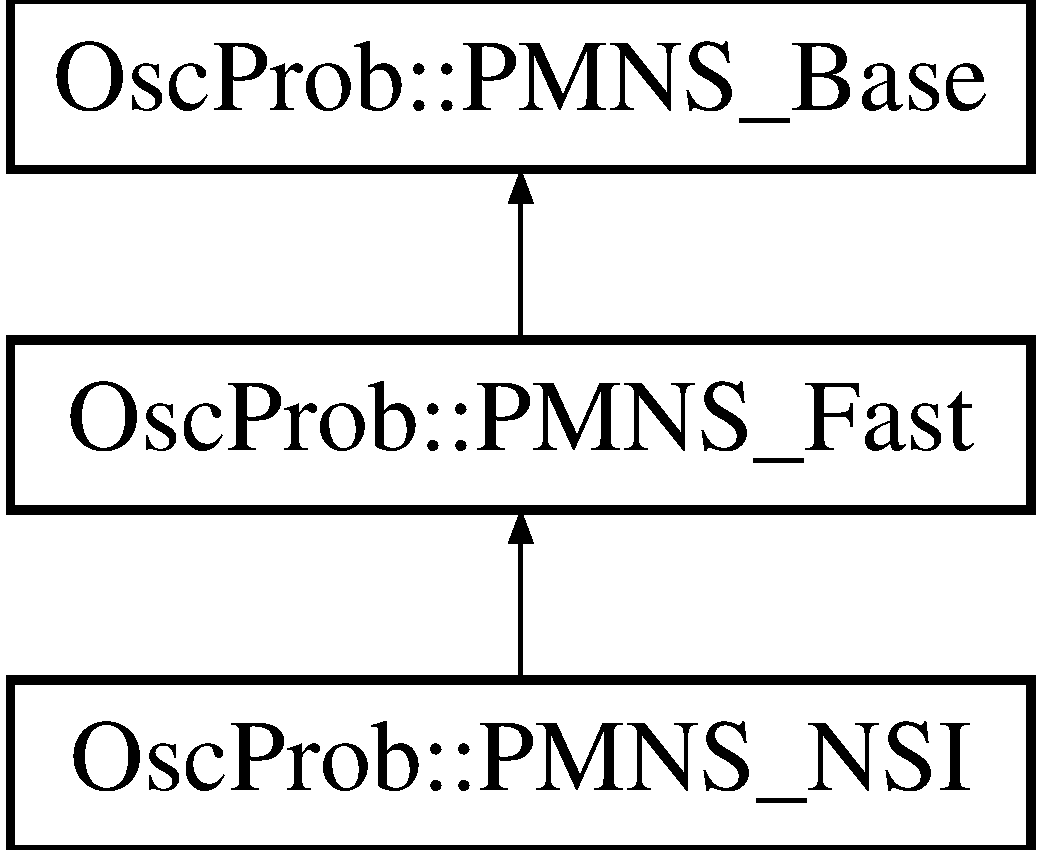
\includegraphics[height=3.000000cm]{classOscProb_1_1PMNS__NSI}
\end{center}
\end{figure}
\subsection*{Public Member Functions}
\begin{DoxyCompactItemize}
\item 
\hyperlink{classOscProb_1_1PMNS__NSI_ab41e79fb427c7a5662443acad31ce7e9}{P\+M\+N\+S\+\_\+\+N\+SI} ()
\begin{DoxyCompactList}\small\item\em Constructor. \end{DoxyCompactList}\item 
virtual \hyperlink{classOscProb_1_1PMNS__NSI_aad1035cb0fb26994029c25b475ec3bde}{$\sim$\+P\+M\+N\+S\+\_\+\+N\+SI} ()
\begin{DoxyCompactList}\small\item\em Destructor. \end{DoxyCompactList}\item 
virtual void \hyperlink{classOscProb_1_1PMNS__NSI_a87c508149ea36b6de493a6817247a0ea}{Set\+Eps} (int flvi, int flvj, double val, double phase)
\begin{DoxyCompactList}\small\item\em Set any given N\+SI parameter. \end{DoxyCompactList}\item 
virtual \hyperlink{EigenPoint_8h_a67ca8e107e20610c3fff78d5e726ece0}{complexD} \hyperlink{classOscProb_1_1PMNS__NSI_a70f1c7d3d0dea3abf8ac40f856fc18ab}{Get\+Eps} (int flvi, int flvj)
\begin{DoxyCompactList}\small\item\em Get any given N\+SI parameter. \end{DoxyCompactList}\item 
void \hyperlink{classOscProb_1_1PMNS__NSI_ae8829af10bc4051e8c74c8b1bc81c88c}{Set\+N\+SI} (double eps\+\_\+ee, double eps\+\_\+emu, double eps\+\_\+etau, double eps\+\_\+mumu, double eps\+\_\+mutau, double eps\+\_\+tautau, double delta\+\_\+emu=0, double delta\+\_\+etau=0, double delta\+\_\+mutau=0)
\begin{DoxyCompactList}\small\item\em Set the N\+SI parameters all at once. \end{DoxyCompactList}\item 
virtual void \hyperlink{classOscProb_1_1PMNS__NSI_a13ecb89c4d43924d23833a9e930f50e0}{Set\+Eps\+\_\+ee} (double a)
\begin{DoxyCompactList}\small\item\em Set eps\+\_\+ee parameter. \end{DoxyCompactList}\item 
virtual void \hyperlink{classOscProb_1_1PMNS__NSI_abf049db9904c745f04346d0d1dedf998}{Set\+Eps\+\_\+mumu} (double a)
\begin{DoxyCompactList}\small\item\em Set eps\+\_\+mumu parameter. \end{DoxyCompactList}\item 
virtual void \hyperlink{classOscProb_1_1PMNS__NSI_a5736f3cd792a621dfa844c3fa314cd17}{Set\+Eps\+\_\+tautau} (double a)
\begin{DoxyCompactList}\small\item\em Set eps\+\_\+tautau parameter. \end{DoxyCompactList}\item 
virtual void \hyperlink{classOscProb_1_1PMNS__NSI_ad5fccd151aea7c673c516b8686f8253c}{Set\+Eps\+\_\+emu} (double a, double phi)
\begin{DoxyCompactList}\small\item\em Set eps\+\_\+emu parameter. \end{DoxyCompactList}\item 
virtual void \hyperlink{classOscProb_1_1PMNS__NSI_a73d43e6d267975d1545af922f8e81bb3}{Set\+Eps\+\_\+etau} (double a, double phi)
\begin{DoxyCompactList}\small\item\em Set eps\+\_\+etau parameter. \end{DoxyCompactList}\item 
virtual void \hyperlink{classOscProb_1_1PMNS__NSI_acfb9893697e04fcc25915ffaf8ed137f}{Set\+Eps\+\_\+mutau} (double a, double phi)
\begin{DoxyCompactList}\small\item\em Set eps\+\_\+mutau parameter. \end{DoxyCompactList}\item 
virtual void \hyperlink{classOscProb_1_1PMNS__NSI_a8e07f5fe44e9ed471efa8e683584e2c7}{Set\+Elec\+Coup} (double e)
\begin{DoxyCompactList}\small\item\em Set electron coupling. \end{DoxyCompactList}\item 
virtual void \hyperlink{classOscProb_1_1PMNS__NSI_a27ecfa2a97c67e6bfb399eeba956f74f}{Set\+Up\+Coup} (double u)
\begin{DoxyCompactList}\small\item\em Set u-\/quark couling. \end{DoxyCompactList}\item 
virtual void \hyperlink{classOscProb_1_1PMNS__NSI_abcc85b0662bd6d08fc5a0bc713657129}{Set\+Down\+Coup} (double d)
\begin{DoxyCompactList}\small\item\em Set d-\/quark couling. \end{DoxyCompactList}\item 
virtual void \hyperlink{classOscProb_1_1PMNS__NSI_a78983619968493630c48080bea9af05e}{Set\+Ferm\+Coup} (double e, double u, double d)
\begin{DoxyCompactList}\small\item\em Set all fermion couplings. \end{DoxyCompactList}\item 
virtual void \hyperlink{classOscProb_1_1PMNS__NSI_a276d475bbebcdf24502a5555ee65b136}{Set\+Coup\+By\+Index} (double c, int i)
\begin{DoxyCompactList}\small\item\em Set a given fermion coupling. \end{DoxyCompactList}\item 
virtual double \hyperlink{classOscProb_1_1PMNS__NSI_adbee38997ab80f8d1a9750d3eae0afea}{Get\+Elec\+Coup} ()
\begin{DoxyCompactList}\small\item\em Get electron coupling. \end{DoxyCompactList}\item 
virtual double \hyperlink{classOscProb_1_1PMNS__NSI_a5fbeeb25bd00fbda7c484dbdb6748a58}{Get\+Up\+Coup} ()
\begin{DoxyCompactList}\small\item\em Get u-\/quark couling. \end{DoxyCompactList}\item 
virtual double \hyperlink{classOscProb_1_1PMNS__NSI_a4f5306674397d6183214d53bf2f110f7}{Get\+Down\+Coup} ()
\begin{DoxyCompactList}\small\item\em Get d-\/quark couling. \end{DoxyCompactList}\item 
virtual double \hyperlink{classOscProb_1_1PMNS__NSI_a42b2db6f2f42dbca7545a10d101a7950}{Get\+Zo\+A\+Coup} ()
\begin{DoxyCompactList}\small\item\em Get effective Z/A coupling. \end{DoxyCompactList}\item 
virtual void \hyperlink{classOscProb_1_1PMNS__Fast_ad849b2231d99c5d66fb3ade8efb896e1}{Set\+Mix} (double th12, double th23, double th13, double deltacp)
\begin{DoxyCompactList}\small\item\em Set the all mixing parameters at once. \end{DoxyCompactList}\item 
virtual void \hyperlink{classOscProb_1_1PMNS__Fast_a63733b246e6d2e609ce3de7a65ba5b9f}{Set\+Delta\+Msqrs} (double dm21, double dm32)
\begin{DoxyCompactList}\small\item\em Set both mass-\/splittings at once. \end{DoxyCompactList}\item 
virtual double \hyperlink{classOscProb_1_1PMNS__Base_aa2e10704d2d205a1ec8988de14b1a66f}{Prob} (std\+::vector$<$ \hyperlink{EigenPoint_8h_a67ca8e107e20610c3fff78d5e726ece0}{complexD} $>$ nu\+\_\+in, int flvf)
\begin{DoxyCompactList}\small\item\em Compute the probability of nu\+\_\+in going to flvf. \end{DoxyCompactList}\item 
virtual double \hyperlink{classOscProb_1_1PMNS__Base_a0190a79284289aacf682c78d7cef9a81}{Prob} (std\+::vector$<$ \hyperlink{EigenPoint_8h_a67ca8e107e20610c3fff78d5e726ece0}{complexD} $>$ nu\+\_\+in, int flvf, double E)
\begin{DoxyCompactList}\small\item\em Compute the probability of nu\+\_\+in going to flvf for energy E. \end{DoxyCompactList}\item 
virtual double \hyperlink{classOscProb_1_1PMNS__Base_a01fba31729345376705e02408e835f67}{Prob} (std\+::vector$<$ \hyperlink{EigenPoint_8h_a67ca8e107e20610c3fff78d5e726ece0}{complexD} $>$ nu\+\_\+in, int flvf, double E, double L)
\begin{DoxyCompactList}\small\item\em Compute the probability of nu\+\_\+in going to flvf for energy E and distance L. \end{DoxyCompactList}\item 
virtual double \hyperlink{classOscProb_1_1PMNS__Base_aec5c399b93261f1962a4b7dbbb44b973}{Prob} (int flvi, int flvf)
\begin{DoxyCompactList}\small\item\em Compute the probability of flvi going to flvf. \end{DoxyCompactList}\item 
virtual double \hyperlink{classOscProb_1_1PMNS__Base_aa3cee10639d5c0879ccb9e78d62128d3}{Prob} (int flvi, int flvf, double E)
\begin{DoxyCompactList}\small\item\em Compute the probability of flvi going to flvf for energy E. \end{DoxyCompactList}\item 
virtual double \hyperlink{classOscProb_1_1PMNS__Base_a6e0a74508d9d6db7be02e242b8467563}{Prob} (int flvi, int flvf, double E, double L)
\begin{DoxyCompactList}\small\item\em Compute the probability of flvi going to flvf for energy E and distance L. \end{DoxyCompactList}\item 
virtual double \hyperlink{classOscProb_1_1PMNS__Base_a89e54c80ae8a31effbab7b2b970606bb}{Avg\+Prob} (std\+::vector$<$ \hyperlink{EigenPoint_8h_a67ca8e107e20610c3fff78d5e726ece0}{complexD} $>$ nu\+\_\+in, int flvf, double E, double dE=0)
\begin{DoxyCompactList}\small\item\em Compute the average probability over a bin of energy. \end{DoxyCompactList}\item 
virtual double \hyperlink{classOscProb_1_1PMNS__Base_ac03f754160422e6600da8dbae0f803ed}{Avg\+Prob} (int flvi, int flvf, double E, double dE=0)
\begin{DoxyCompactList}\small\item\em Compute the average probability over a bin of energy. \end{DoxyCompactList}\item 
virtual double \hyperlink{classOscProb_1_1PMNS__Base_a19f160c045a01e5083506e925fb37d44}{Avg\+Prob\+LoE} (std\+::vector$<$ \hyperlink{EigenPoint_8h_a67ca8e107e20610c3fff78d5e726ece0}{complexD} $>$ nu\+\_\+in, int flvf, double LoE, double d\+LoE=0)
\begin{DoxyCompactList}\small\item\em Compute the average probability over a bin of L/E. \end{DoxyCompactList}\item 
virtual double \hyperlink{classOscProb_1_1PMNS__Base_ac19a92f4ef428a7333ca8eed76fca637}{Avg\+Prob\+LoE} (int flvi, int flvf, double LoE, double d\+LoE=0)
\begin{DoxyCompactList}\small\item\em Compute the average probability over a bin of L/E. \end{DoxyCompactList}\item 
virtual std\+::vector$<$ \hyperlink{EigenPoint_8h_a67ca8e107e20610c3fff78d5e726ece0}{complexD} $>$ \hyperlink{classOscProb_1_1PMNS__Base_a5092561dd8579d390c649eb60803ea98}{Get\+Mass\+Eigenstate} (int mi)
\begin{DoxyCompactList}\small\item\em Get a neutrino mass eigenstate. \end{DoxyCompactList}\item 
virtual void \hyperlink{classOscProb_1_1PMNS__Base_ace7875cf6d3bec161a2b7ed2690aec34}{Set\+Angle} (int i, int j, double th)
\begin{DoxyCompactList}\small\item\em Set the mixing angle theta\+\_\+ij. \end{DoxyCompactList}\item 
virtual void \hyperlink{classOscProb_1_1PMNS__Base_a4bef78cfcfc4e70b4ce79cdb8862c0a3}{Set\+Delta} (int i, int j, double delta)
\begin{DoxyCompactList}\small\item\em Set the CP phase delta\+\_\+ij. \end{DoxyCompactList}\item 
virtual void \hyperlink{classOscProb_1_1PMNS__Base_a492243b22fb1b783cd2943f507cff970}{Set\+Dm} (int j, double dm)
\begin{DoxyCompactList}\small\item\em Set the mass-\/splitting dm\+\_\+j1 in e\+V$^\wedge$2. \end{DoxyCompactList}\item 
virtual double \hyperlink{classOscProb_1_1PMNS__Base_acee137091304c919642293ddf015bbc8}{Get\+Angle} (int i, int j)
\begin{DoxyCompactList}\small\item\em Get the mixing angle theta\+\_\+ij. \end{DoxyCompactList}\item 
virtual double \hyperlink{classOscProb_1_1PMNS__Base_adb8dbc91d4286d2e7c8f768c59476241}{Get\+Delta} (int i, int j)
\begin{DoxyCompactList}\small\item\em Get the CP phase delta\+\_\+ij. \end{DoxyCompactList}\item 
virtual double \hyperlink{classOscProb_1_1PMNS__Base_ad26815ac5f4805d1259817e4936e5f8f}{Get\+Dm} (int j)
\begin{DoxyCompactList}\small\item\em Get the mass-\/splitting dm\+\_\+j1 in e\+V$^\wedge$2. \end{DoxyCompactList}\item 
virtual double \hyperlink{classOscProb_1_1PMNS__Base_a4ea861a6707ce1be3a54aad2b60f8632}{Get\+Dm\+Eff} (int j)
\begin{DoxyCompactList}\small\item\em Get the effective mass-\/splitting dm\+\_\+j1 in e\+V$^\wedge$2. \end{DoxyCompactList}\item 
virtual void \hyperlink{classOscProb_1_1PMNS__Base_a4de96ac9b6d1e9b029ab877e57d211ad}{Set\+Std\+Pars} ()
\begin{DoxyCompactList}\small\item\em Set P\+DG 3-\/flavor parameters. \end{DoxyCompactList}\item 
virtual void \hyperlink{classOscProb_1_1PMNS__Base_a95b3b0d0cab5e6a54b5ef99587f837c0}{Set\+Energy} (double E)
\begin{DoxyCompactList}\small\item\em Set the neutrino energy in GeV. \end{DoxyCompactList}\item 
virtual void \hyperlink{classOscProb_1_1PMNS__Base_a717e0348cf762f3961854e332a9b52e0}{Set\+Is\+Nu\+Bar} (bool is\+Nu\+Bar)
\begin{DoxyCompactList}\small\item\em Set the anti-\/neutrino flag. \end{DoxyCompactList}\item 
virtual double \hyperlink{classOscProb_1_1PMNS__Base_acc0d46cc4b8f911b40b807225003bbed}{Get\+Energy} ()
\begin{DoxyCompactList}\small\item\em Get the neutrino energy in GeV. \end{DoxyCompactList}\item 
virtual bool \hyperlink{classOscProb_1_1PMNS__Base_a2f7f2a028dfe7a90fff6b4f757972c2c}{Get\+Is\+Nu\+Bar} ()
\begin{DoxyCompactList}\small\item\em Get the anti-\/neutrino flag. \end{DoxyCompactList}\item 
virtual void \hyperlink{classOscProb_1_1PMNS__Base_ac3b644fd0a56347d304ceca4ae9d8875}{Set\+Path} (\hyperlink{structOscProb_1_1NuPath}{Osc\+Prob\+::\+Nu\+Path} p)
\begin{DoxyCompactList}\small\item\em Set a single path. \end{DoxyCompactList}\item 
virtual void \hyperlink{classOscProb_1_1PMNS__Base_a35b983270613072a3df58b574d80dbfd}{Set\+Path} (double length, double density, double zoa=0.\+5, int layer=0)
\begin{DoxyCompactList}\small\item\em Set a single path. \end{DoxyCompactList}\item 
virtual void \hyperlink{classOscProb_1_1PMNS__Base_a637d19dd850b4246507796526622643c}{Set\+Path} (std\+::vector$<$ \hyperlink{structOscProb_1_1NuPath}{Osc\+Prob\+::\+Nu\+Path} $>$ paths)
\begin{DoxyCompactList}\small\item\em Set a path sequence. \end{DoxyCompactList}\item 
virtual void \hyperlink{classOscProb_1_1PMNS__Base_a887dc9d4dc569ec0cdef3933b4c60efc}{Add\+Path} (\hyperlink{structOscProb_1_1NuPath}{Osc\+Prob\+::\+Nu\+Path} p)
\begin{DoxyCompactList}\small\item\em Add a path to the sequence. \end{DoxyCompactList}\item 
virtual void \hyperlink{classOscProb_1_1PMNS__Base_ab7f89ad9e7e1224adaa59d3c41594cd9}{Add\+Path} (double length, double density, double zoa=0.\+5, int layer=0)
\begin{DoxyCompactList}\small\item\em Add a path to the sequence. \end{DoxyCompactList}\item 
virtual void \hyperlink{classOscProb_1_1PMNS__Base_aefe521239031c418cfaaaa550a6e13bb}{Clear\+Path} ()
\begin{DoxyCompactList}\small\item\em Clear the path vector. \end{DoxyCompactList}\item 
virtual void \hyperlink{classOscProb_1_1PMNS__Base_a6241325b1bd28cafa556daaecbe4ed62}{Set\+Length} (double L)
\begin{DoxyCompactList}\small\item\em Set a single path lentgh in km. \end{DoxyCompactList}\item 
virtual void \hyperlink{classOscProb_1_1PMNS__Base_aa34a40a3b5abda0f252982d9ead3b520}{Set\+Length} (std\+::vector$<$ double $>$ L)
\begin{DoxyCompactList}\small\item\em Set multiple path lengths. \end{DoxyCompactList}\item 
virtual void \hyperlink{classOscProb_1_1PMNS__Base_ac74206f349687da141392c81e2ba6b0d}{Set\+Density} (double rho)
\begin{DoxyCompactList}\small\item\em Set single path density in g/cm$^\wedge$3. \end{DoxyCompactList}\item 
virtual void \hyperlink{classOscProb_1_1PMNS__Base_a858221d5510fe732dc6a101fd305cda0}{Set\+Density} (std\+::vector$<$ double $>$ rho)
\begin{DoxyCompactList}\small\item\em Set multiple path densities. \end{DoxyCompactList}\item 
virtual void \hyperlink{classOscProb_1_1PMNS__Base_a1bf3ea8fd2507fd2fd82d7410ff8f578}{Set\+ZoA} (double zoa)
\begin{DoxyCompactList}\small\item\em Set Z/A value for single path. \end{DoxyCompactList}\item 
virtual void \hyperlink{classOscProb_1_1PMNS__Base_a8495f8a320e1a21965e6a64aec92ad2a}{Set\+ZoA} (std\+::vector$<$ double $>$ zoa)
\begin{DoxyCompactList}\small\item\em Set multiple path Z/A values. \end{DoxyCompactList}\item 
virtual void \hyperlink{classOscProb_1_1PMNS__Base_a904e580edf89fb98bf9a6397739b4ebe}{Set\+Layers} (std\+::vector$<$ int $>$ lay)
\begin{DoxyCompactList}\small\item\em Set multiple path layer indices. \end{DoxyCompactList}\item 
virtual void \hyperlink{classOscProb_1_1PMNS__Base_add6533a9fc9acdfc7ae258b62570d78d}{Set\+Std\+Path} ()
\begin{DoxyCompactList}\small\item\em Set standard neutrino path. \end{DoxyCompactList}\item 
virtual std\+::vector$<$ \hyperlink{structOscProb_1_1NuPath}{Osc\+Prob\+::\+Nu\+Path} $>$ \hyperlink{classOscProb_1_1PMNS__Base_ac8e196f2e85a2b1caaf705073ee95a5c}{Get\+Path} ()
\begin{DoxyCompactList}\small\item\em Get the neutrino path sequence. \end{DoxyCompactList}\item 
virtual std\+::vector$<$ double $>$ \hyperlink{classOscProb_1_1PMNS__Base_a9eac8d768c1424755ee41f7e783af179}{Get\+Sample\+Points} (double LoE, double d\+LoE)
\begin{DoxyCompactList}\small\item\em Compute the sample points for a bin of L/E with width d\+LoE. \end{DoxyCompactList}\item 
virtual void \hyperlink{classOscProb_1_1PMNS__Base_aa94c1e1fff0ba731c75f7e633b023a9f}{Set\+Use\+Cache} (bool u=true)
\begin{DoxyCompactList}\small\item\em Set caching on/off. \end{DoxyCompactList}\item 
virtual void \hyperlink{classOscProb_1_1PMNS__Base_ac47fd33e69aa6490f99e2fd147a92f03}{Clear\+Cache} ()
\begin{DoxyCompactList}\small\item\em Clear the cache. \end{DoxyCompactList}\item 
virtual void \hyperlink{classOscProb_1_1PMNS__Base_ae67862cf58b0802487a14b047b012a78}{Set\+Max\+Cache} (int mc=1e6)
\begin{DoxyCompactList}\small\item\em Set max cache size. \end{DoxyCompactList}\end{DoxyCompactItemize}
\subsection*{Protected Member Functions}
\begin{DoxyCompactItemize}
\item 
virtual void \hyperlink{classOscProb_1_1PMNS__NSI_ab5c4f4644fbedb8835f6336c553805ce}{Update\+Ham} ()
\begin{DoxyCompactList}\small\item\em Build the full Hamiltonian. \end{DoxyCompactList}\item 
virtual void \hyperlink{classOscProb_1_1PMNS__Fast_a8a0828401591e88c60e0051fbfe02d5e}{Solve\+Ham} ()
\begin{DoxyCompactList}\small\item\em Solve the full Hamiltonian for eigenvectors and eigenvalues. \end{DoxyCompactList}\item 
virtual void \hyperlink{classOscProb_1_1PMNS__Fast_a76dd5a761df8689c502b28ad0391f9e2}{Set\+Vacuum\+Eigensystem} ()
\begin{DoxyCompactList}\small\item\em Set the eigensystem to the analytic solution of the vacuum Hamiltonian. \end{DoxyCompactList}\item 
virtual void \hyperlink{classOscProb_1_1PMNS__Base_adf23b569112f9f9e0e592f01d79a5f3d}{Initialize\+Vectors} ()
\begin{DoxyCompactList}\small\item\em Initialize all member vectors with zeros. \end{DoxyCompactList}\item 
virtual bool \hyperlink{classOscProb_1_1PMNS__Base_abe533da5f64bec1f4724ab7b58606b77}{Try\+Cache} ()
\begin{DoxyCompactList}\small\item\em Try to find a cached eigensystem. \end{DoxyCompactList}\item 
virtual void \hyperlink{classOscProb_1_1PMNS__Base_a785c37fcea974628623c8881bb0fbbf9}{Fill\+Cache} ()
\begin{DoxyCompactList}\small\item\em Cache the current eigensystem. \end{DoxyCompactList}\item 
virtual void \hyperlink{classOscProb_1_1PMNS__Base_a986e6ebef09a7e2eb7fee16a4c2c834d}{Set\+Cur\+Path} (\hyperlink{structOscProb_1_1NuPath}{Osc\+Prob\+::\+Nu\+Path} p)
\begin{DoxyCompactList}\small\item\em Set the path currently in use by the class. \end{DoxyCompactList}\item 
virtual void \hyperlink{classOscProb_1_1PMNS__Base_aba565962a440d14bee7a2a96d2eca2c5}{Set\+Att} (double att, int idx)
\begin{DoxyCompactList}\small\item\em Set one of the path attributes. \end{DoxyCompactList}\item 
virtual void \hyperlink{classOscProb_1_1PMNS__Base_aa001479b5f5828c3d16ed087f96ecbcc}{Set\+Att} (std\+::vector$<$ double $>$ att, int idx)
\begin{DoxyCompactList}\small\item\em Set all values of a path attribute. \end{DoxyCompactList}\item 
virtual void \hyperlink{classOscProb_1_1PMNS__Base_a6a3cf45bbe2349abf06708b65677c044}{RotateH} (int i, int j, std\+::vector$<$ std\+::vector$<$ \hyperlink{EigenPoint_8h_a67ca8e107e20610c3fff78d5e726ece0}{complexD} $>$ $>$ \&Ham)
\begin{DoxyCompactList}\small\item\em Rotate the Hamiltonian by theta\+\_\+ij and delta\+\_\+ij. \end{DoxyCompactList}\item 
virtual void \hyperlink{classOscProb_1_1PMNS__Base_ae52554477ad3250daa5adb8c32cab0b4}{Rotate\+State} (int i, int j)
\begin{DoxyCompactList}\small\item\em Rotate the neutrino state by theta\+\_\+ij and delta\+\_\+ij. \end{DoxyCompactList}\item 
virtual void \hyperlink{classOscProb_1_1PMNS__Base_ad0faf5eae755afb1baa1fcd5ffebad41}{Build\+Hms} ()
\begin{DoxyCompactList}\small\item\em Build the matrix of masses squared. \end{DoxyCompactList}\item 
virtual void \hyperlink{classOscProb_1_1PMNS__Base_ac0d4bf8ff1318ef96d3dafa62e0cec25}{Reset\+To\+Flavour} (int flv)
\begin{DoxyCompactList}\small\item\em Reset neutrino state to pure flavour flv. \end{DoxyCompactList}\item 
virtual void \hyperlink{classOscProb_1_1PMNS__Base_accb08503acc162188041d7a96a280462}{Propagate\+Path} (\hyperlink{structOscProb_1_1NuPath}{Osc\+Prob\+::\+Nu\+Path} p)
\begin{DoxyCompactList}\small\item\em Propagate neutrino through a single path. \end{DoxyCompactList}\item 
virtual void \hyperlink{classOscProb_1_1PMNS__Base_a054e3a8b05b9a958b6fa416e4a835e3e}{Propagate} ()
\begin{DoxyCompactList}\small\item\em Propagate neutrino through full path. \end{DoxyCompactList}\item 
virtual double \hyperlink{classOscProb_1_1PMNS__Base_a0dc4d45bc3d7e03b9abbf5b4e100cc22}{P} (int flv)
\begin{DoxyCompactList}\small\item\em Return the probability of final state in flavour flv. \end{DoxyCompactList}\end{DoxyCompactItemize}
\subsection*{Protected Attributes}
\begin{DoxyCompactItemize}
\item 
\hyperlink{EigenPoint_8h_a67ca8e107e20610c3fff78d5e726ece0}{complexD} \hyperlink{classOscProb_1_1PMNS__NSI_ab9328cb72e868b395f3efdd75b6af5e4}{f\+Eps} \mbox{[}3\mbox{]}\mbox{[}3\mbox{]}
\begin{DoxyCompactList}\small\item\em Stores each N\+SI parameter. \end{DoxyCompactList}\item 
double \hyperlink{classOscProb_1_1PMNS__NSI_a1ac51957bbc4cec9fcfd8f816491cc95}{f\+N\+S\+Icoup} \mbox{[}3\mbox{]}
\begin{DoxyCompactList}\small\item\em Relative N\+SI couplings. \end{DoxyCompactList}\item 
\hyperlink{EigenPoint_8h_a67ca8e107e20610c3fff78d5e726ece0}{complexD} \hyperlink{classOscProb_1_1PMNS__Fast_a94286a881bc53dd512a89d548346b611}{f\+Ham} \mbox{[}3\mbox{]}\mbox{[}3\mbox{]}
\begin{DoxyCompactList}\small\item\em The full hamiltonian. \end{DoxyCompactList}\item 
int \hyperlink{classOscProb_1_1PMNS__Base_a24bb74bed63569dfe88b18fa6a08060e}{f\+Num\+Nus}
\begin{DoxyCompactList}\small\item\em Number of neutrino flavours. \end{DoxyCompactList}\item 
std\+::vector$<$ double $>$ \hyperlink{classOscProb_1_1PMNS__Base_a406a31c3b5d620e5a0cace5b411f9f70}{f\+Dm}
\begin{DoxyCompactList}\small\item\em m$^\wedge$2\+\_\+i -\/ m$^\wedge$2\+\_\+1 in vacuum \end{DoxyCompactList}\item 
std\+::vector$<$ std\+::vector$<$ double $>$ $>$ \hyperlink{classOscProb_1_1PMNS__Base_a1976887cd658dd86b2336c181f1470b4}{f\+Theta}
\begin{DoxyCompactList}\small\item\em theta\mbox{[}i\mbox{]}\mbox{[}j\mbox{]} mixing angle \end{DoxyCompactList}\item 
std\+::vector$<$ std\+::vector$<$ double $>$ $>$ \hyperlink{classOscProb_1_1PMNS__Base_ab2a5fa40e689b221c8a7d2c17213810d}{f\+Delta}
\begin{DoxyCompactList}\small\item\em delta\mbox{[}i\mbox{]}\mbox{[}j\mbox{]} CP violating phase \end{DoxyCompactList}\item 
std\+::vector$<$ \hyperlink{EigenPoint_8h_a67ca8e107e20610c3fff78d5e726ece0}{complexD} $>$ \hyperlink{classOscProb_1_1PMNS__Base_abf99f2339e3ee989600740b5d88063e8}{f\+Nu\+State}
\begin{DoxyCompactList}\small\item\em The neutrino current state. \end{DoxyCompactList}\item 
std\+::vector$<$ std\+::vector$<$ \hyperlink{EigenPoint_8h_a67ca8e107e20610c3fff78d5e726ece0}{complexD} $>$ $>$ \hyperlink{classOscProb_1_1PMNS__Base_acd3c8783e7603081eab316ea4c86c766}{f\+Hms}
\begin{DoxyCompactList}\small\item\em matrix H$\ast$2E in e\+V$^\wedge$2 \end{DoxyCompactList}\item 
std\+::vector$<$ \hyperlink{EigenPoint_8h_a67ca8e107e20610c3fff78d5e726ece0}{complexD} $>$ \hyperlink{classOscProb_1_1PMNS__Base_ab8d26b722047d49d977f5f2d83026ede}{f\+Phases}
\begin{DoxyCompactList}\small\item\em Buffer for oscillation phases. \end{DoxyCompactList}\item 
std\+::vector$<$ \hyperlink{EigenPoint_8h_a67ca8e107e20610c3fff78d5e726ece0}{complexD} $>$ \hyperlink{classOscProb_1_1PMNS__Base_a5440bc3efa466a37649601abce559e3e}{f\+Buffer}
\begin{DoxyCompactList}\small\item\em Buffer for neutrino state tranformations. \end{DoxyCompactList}\item 
std\+::vector$<$ double $>$ \hyperlink{classOscProb_1_1PMNS__Base_a6319c34d7decbb9d7d6da279c06e8c2d}{f\+Eval}
\begin{DoxyCompactList}\small\item\em Eigenvalues of the Hamiltonian. \end{DoxyCompactList}\item 
std\+::vector$<$ std\+::vector$<$ \hyperlink{EigenPoint_8h_a67ca8e107e20610c3fff78d5e726ece0}{complexD} $>$ $>$ \hyperlink{classOscProb_1_1PMNS__Base_a87be137356c5f27ab83cab5e1298ef8f}{f\+Evec}
\begin{DoxyCompactList}\small\item\em Eigenvectors of the Hamiltonian. \end{DoxyCompactList}\item 
double \hyperlink{classOscProb_1_1PMNS__Base_a2800af6d436972f3e900867790c046b0}{f\+Energy}
\begin{DoxyCompactList}\small\item\em Neutrino energy. \end{DoxyCompactList}\item 
bool \hyperlink{classOscProb_1_1PMNS__Base_a0ebaeaefab36a3ff381c6293faedfdd6}{f\+Is\+Nu\+Bar}
\begin{DoxyCompactList}\small\item\em Anti-\/neutrino flag. \end{DoxyCompactList}\item 
std\+::vector$<$ \hyperlink{structOscProb_1_1NuPath}{Osc\+Prob\+::\+Nu\+Path} $>$ \hyperlink{classOscProb_1_1PMNS__Base_a69db9d57e12fc7cbe0431bc6c18fac93}{f\+Nu\+Paths}
\begin{DoxyCompactList}\small\item\em Vector of neutrino paths. \end{DoxyCompactList}\item 
\hyperlink{structOscProb_1_1NuPath}{Osc\+Prob\+::\+Nu\+Path} \hyperlink{classOscProb_1_1PMNS__Base_a849437aa8891fe042e86886ce8f81c6e}{f\+Path}
\begin{DoxyCompactList}\small\item\em Current neutrino path. \end{DoxyCompactList}\item 
bool \hyperlink{classOscProb_1_1PMNS__Base_a9ac3cadeac8db1b90f3152f476244780}{f\+Built\+Hms}
\begin{DoxyCompactList}\small\item\em Tag to avoid rebuilding Hms. \end{DoxyCompactList}\item 
bool \hyperlink{classOscProb_1_1PMNS__Base_a6dc5cd010d2d70b2324745b4e53e9839}{f\+Got\+ES}
\begin{DoxyCompactList}\small\item\em Tag to avoid recalculating eigensystem. \end{DoxyCompactList}\item 
bool \hyperlink{classOscProb_1_1PMNS__Base_ad28c12ef897b5555eda509ea55c99107}{f\+Use\+Cache}
\begin{DoxyCompactList}\small\item\em Flag for whether to use caching. \end{DoxyCompactList}\item 
double \hyperlink{classOscProb_1_1PMNS__Base_a0b4c41a27de281472453a1912cbc1e64}{f\+Cache\+Prec}
\begin{DoxyCompactList}\small\item\em Precision of cache matching. \end{DoxyCompactList}\item 
int \hyperlink{classOscProb_1_1PMNS__Base_a74c13356eafec2490d8c3c19759ba7f0}{f\+Max\+Cache}
\begin{DoxyCompactList}\small\item\em Maximum cache size. \end{DoxyCompactList}\item 
std\+::set$<$ \hyperlink{structOscProb_1_1EigenPoint}{Osc\+Prob\+::\+Eigen\+Point} $>$ \hyperlink{classOscProb_1_1PMNS__Base_a8159424f20197a3a7145fe3bf2c11176}{f\+Mix\+Cache}
\begin{DoxyCompactList}\small\item\em Caching set of eigensystems. \end{DoxyCompactList}\item 
\hyperlink{structOscProb_1_1EigenPoint}{Eigen\+Point} \hyperlink{classOscProb_1_1PMNS__Base_ab1fe4800ee3ae48df4fc942dce00e0d3}{f\+Probe}
\begin{DoxyCompactList}\small\item\em Eigenp\+Point to try. \end{DoxyCompactList}\end{DoxyCompactItemize}
\subsection*{Static Protected Attributes}
\begin{DoxyCompactItemize}
\item 
static const \hyperlink{EigenPoint_8h_a67ca8e107e20610c3fff78d5e726ece0}{complexD} \hyperlink{classOscProb_1_1PMNS__Base_a05e595848c2521dc795efa7645728b94}{zero}
\begin{DoxyCompactList}\small\item\em zero in complex \end{DoxyCompactList}\item 
static const \hyperlink{EigenPoint_8h_a67ca8e107e20610c3fff78d5e726ece0}{complexD} \hyperlink{classOscProb_1_1PMNS__Base_a7d1d0bbcab30a1fd8c368c40134c51ff}{one}
\begin{DoxyCompactList}\small\item\em one in complex \end{DoxyCompactList}\item 
static const double \hyperlink{classOscProb_1_1PMNS__Base_a382ddd7b76ca89b43f22614a2ea7327b}{k\+Km2eV} = 1.\+0 / 1.\+973269788e-\/10
\begin{DoxyCompactList}\small\item\em km to e\+V$^\wedge$-\/1 \end{DoxyCompactList}\item 
static const double \hyperlink{classOscProb_1_1PMNS__Base_a326fc5016d7dd7ce05682c06cdcb6d94}{k\+K2} = 1e-\/3 $\ast$ k\+N\+A / pow(k\+Km2e\+V,3)
\begin{DoxyCompactList}\small\item\em mol/\+Ge\+V$^\wedge$2/cm$^\wedge$3 to eV \end{DoxyCompactList}\item 
static const double \hyperlink{classOscProb_1_1PMNS__Base_ad36a0a6bf58d6ec093d3947784bd89e9}{k\+Ge\+V2eV} = 1.\+0e+09
\begin{DoxyCompactList}\small\item\em GeV to eV. \end{DoxyCompactList}\item 
static const double \hyperlink{classOscProb_1_1PMNS__Base_a69355e770b89e99437c2b8a66e48eeb9}{k\+NA} = 6.\+022140857e23
\begin{DoxyCompactList}\small\item\em Avogadro constant. \end{DoxyCompactList}\item 
static const double \hyperlink{classOscProb_1_1PMNS__Base_a7f26a3456128234b2ae6cc9141a6532f}{k\+Gf} = 1.\+1663787e-\/05
\begin{DoxyCompactList}\small\item\em G\+\_\+F in units of Ge\+V$^\wedge$-\/2. \end{DoxyCompactList}\end{DoxyCompactItemize}


\subsection{Detailed Description}
This class expands the \hyperlink{classOscProb_1_1PMNS__Fast}{P\+M\+N\+S\+\_\+\+Fast} class including a general matter potential matrix describing Non-\/\+Standard Interactions (N\+SI).

The matter potential is parametrized by dimensionless quantities epsilon which quantify the intensity of the N\+SI with respect to the standard matter effects from coherent forward scattering with electrons.

\begin{DoxySeeAlso}{See also}
\hyperlink{classOscProb_1_1PMNS__Fast}{P\+M\+N\+S\+\_\+\+Fast}
\end{DoxySeeAlso}
\begin{DoxyAuthor}{Author}
coelho@lal.\+in2p3.\+fr 
\end{DoxyAuthor}


Definition at line 25 of file P\+M\+N\+S\+\_\+\+N\+S\+I.\+h.



\subsection{Constructor \& Destructor Documentation}
\mbox{\Hypertarget{classOscProb_1_1PMNS__NSI_ab41e79fb427c7a5662443acad31ce7e9}\label{classOscProb_1_1PMNS__NSI_ab41e79fb427c7a5662443acad31ce7e9}} 
\index{Osc\+Prob\+::\+P\+M\+N\+S\+\_\+\+N\+SI@{Osc\+Prob\+::\+P\+M\+N\+S\+\_\+\+N\+SI}!P\+M\+N\+S\+\_\+\+N\+SI@{P\+M\+N\+S\+\_\+\+N\+SI}}
\index{P\+M\+N\+S\+\_\+\+N\+SI@{P\+M\+N\+S\+\_\+\+N\+SI}!Osc\+Prob\+::\+P\+M\+N\+S\+\_\+\+N\+SI@{Osc\+Prob\+::\+P\+M\+N\+S\+\_\+\+N\+SI}}
\subsubsection{\texorpdfstring{P\+M\+N\+S\+\_\+\+N\+S\+I()}{PMNS\_NSI()}}
{\footnotesize\ttfamily P\+M\+N\+S\+\_\+\+N\+S\+I\+::\+P\+M\+N\+S\+\_\+\+N\+SI (\begin{DoxyParamCaption}{ }\end{DoxyParamCaption})}

Constructor. \begin{DoxySeeAlso}{See also}
\hyperlink{classOscProb_1_1PMNS__Base_aa53e83b03a9cf4bdfa0a07136bd17a79}{P\+M\+N\+S\+\_\+\+Base\+::\+P\+M\+N\+S\+\_\+\+Base}
\end{DoxySeeAlso}
This class is restricted to 3 neutrino flavours. 

Definition at line 29 of file P\+M\+N\+S\+\_\+\+N\+S\+I.\+cxx.



References Set\+Ferm\+Coup(), Set\+N\+S\+I(), and Osc\+Prob\+::\+P\+M\+N\+S\+\_\+\+Base\+::\+Set\+Std\+Path().


\begin{DoxyCode}
29                    : \hyperlink{classOscProb_1_1PMNS__Fast_a2bbac744bf63753105d766a860af7c0d}{PMNS\_Fast}(), \hyperlink{classOscProb_1_1PMNS__NSI_ab9328cb72e868b395f3efdd75b6af5e4}{fEps}()
30 \{
31   \hyperlink{classOscProb_1_1PMNS__Base_add6533a9fc9acdfc7ae258b62570d78d}{SetStdPath}();
32   \hyperlink{classOscProb_1_1PMNS__NSI_ae8829af10bc4051e8c74c8b1bc81c88c}{SetNSI}(0.,0.,0.,0.,0.,0.,0.,0.,0.);
33   \hyperlink{classOscProb_1_1PMNS__NSI_a78983619968493630c48080bea9af05e}{SetFermCoup}(1,0,0);
34 \}
\end{DoxyCode}
\mbox{\Hypertarget{classOscProb_1_1PMNS__NSI_aad1035cb0fb26994029c25b475ec3bde}\label{classOscProb_1_1PMNS__NSI_aad1035cb0fb26994029c25b475ec3bde}} 
\index{Osc\+Prob\+::\+P\+M\+N\+S\+\_\+\+N\+SI@{Osc\+Prob\+::\+P\+M\+N\+S\+\_\+\+N\+SI}!````~P\+M\+N\+S\+\_\+\+N\+SI@{$\sim$\+P\+M\+N\+S\+\_\+\+N\+SI}}
\index{````~P\+M\+N\+S\+\_\+\+N\+SI@{$\sim$\+P\+M\+N\+S\+\_\+\+N\+SI}!Osc\+Prob\+::\+P\+M\+N\+S\+\_\+\+N\+SI@{Osc\+Prob\+::\+P\+M\+N\+S\+\_\+\+N\+SI}}
\subsubsection{\texorpdfstring{$\sim$\+P\+M\+N\+S\+\_\+\+N\+S\+I()}{~PMNS\_NSI()}}
{\footnotesize\ttfamily P\+M\+N\+S\+\_\+\+N\+S\+I\+::$\sim$\+P\+M\+N\+S\+\_\+\+N\+SI (\begin{DoxyParamCaption}{ }\end{DoxyParamCaption})\hspace{0.3cm}{\ttfamily [virtual]}}

Nothing to clean. 

Definition at line 40 of file P\+M\+N\+S\+\_\+\+N\+S\+I.\+cxx.


\begin{DoxyCode}
40 \{\}
\end{DoxyCode}


\subsection{Member Function Documentation}
\mbox{\Hypertarget{classOscProb_1_1PMNS__Base_a887dc9d4dc569ec0cdef3933b4c60efc}\label{classOscProb_1_1PMNS__Base_a887dc9d4dc569ec0cdef3933b4c60efc}} 
\index{Osc\+Prob\+::\+P\+M\+N\+S\+\_\+\+N\+SI@{Osc\+Prob\+::\+P\+M\+N\+S\+\_\+\+N\+SI}!Add\+Path@{Add\+Path}}
\index{Add\+Path@{Add\+Path}!Osc\+Prob\+::\+P\+M\+N\+S\+\_\+\+N\+SI@{Osc\+Prob\+::\+P\+M\+N\+S\+\_\+\+N\+SI}}
\subsubsection{\texorpdfstring{Add\+Path()}{AddPath()}\hspace{0.1cm}{\footnotesize\ttfamily [1/2]}}
{\footnotesize\ttfamily void P\+M\+N\+S\+\_\+\+Base\+::\+Add\+Path (\begin{DoxyParamCaption}\item[{\hyperlink{structOscProb_1_1NuPath}{Osc\+Prob\+::\+Nu\+Path}}]{p }\end{DoxyParamCaption})\hspace{0.3cm}{\ttfamily [virtual]}, {\ttfamily [inherited]}}

Add a path to the sequence. 
\begin{DoxyParams}{Parameters}
{\em p} & -\/ A neutrino path segment \\
\hline
\end{DoxyParams}


Definition at line 351 of file P\+M\+N\+S\+\_\+\+Base.\+cxx.



References Osc\+Prob\+::\+P\+M\+N\+S\+\_\+\+Base\+::f\+Nu\+Paths.



Referenced by Osc\+Prob\+::\+P\+M\+N\+S\+\_\+\+Base\+::\+Add\+Path(), Osc\+Prob\+::\+P\+M\+N\+S\+\_\+\+Base\+::\+Set\+Att(), and Osc\+Prob\+::\+P\+M\+N\+S\+\_\+\+Base\+::\+Set\+Path().


\begin{DoxyCode}
351                                \{
352 
353   \hyperlink{classOscProb_1_1PMNS__Base_a69db9d57e12fc7cbe0431bc6c18fac93}{fNuPaths}.push\_back(p);
354 
355 \}
\end{DoxyCode}
\mbox{\Hypertarget{classOscProb_1_1PMNS__Base_ab7f89ad9e7e1224adaa59d3c41594cd9}\label{classOscProb_1_1PMNS__Base_ab7f89ad9e7e1224adaa59d3c41594cd9}} 
\index{Osc\+Prob\+::\+P\+M\+N\+S\+\_\+\+N\+SI@{Osc\+Prob\+::\+P\+M\+N\+S\+\_\+\+N\+SI}!Add\+Path@{Add\+Path}}
\index{Add\+Path@{Add\+Path}!Osc\+Prob\+::\+P\+M\+N\+S\+\_\+\+N\+SI@{Osc\+Prob\+::\+P\+M\+N\+S\+\_\+\+N\+SI}}
\subsubsection{\texorpdfstring{Add\+Path()}{AddPath()}\hspace{0.1cm}{\footnotesize\ttfamily [2/2]}}
{\footnotesize\ttfamily void P\+M\+N\+S\+\_\+\+Base\+::\+Add\+Path (\begin{DoxyParamCaption}\item[{double}]{length,  }\item[{double}]{density,  }\item[{double}]{zoa = {\ttfamily 0.5},  }\item[{int}]{layer = {\ttfamily 0} }\end{DoxyParamCaption})\hspace{0.3cm}{\ttfamily [virtual]}, {\ttfamily [inherited]}}

Add a path to the sequence defining attributes directly. 
\begin{DoxyParams}{Parameters}
{\em length} & -\/ The length of the path segment in km \\
\hline
{\em density} & -\/ The density of the path segment in g/cm$^\wedge$3 \\
\hline
{\em zoa} & -\/ The effective Z/A of the path segment \\
\hline
{\em layer} & -\/ An index to identify the layer type (e.\+g. earth inner core) \\
\hline
\end{DoxyParams}


Definition at line 365 of file P\+M\+N\+S\+\_\+\+Base.\+cxx.



References Osc\+Prob\+::\+P\+M\+N\+S\+\_\+\+Base\+::\+Add\+Path().


\begin{DoxyCode}
365                                                                            \{
366 
367   \hyperlink{classOscProb_1_1PMNS__Base_a887dc9d4dc569ec0cdef3933b4c60efc}{AddPath}(\hyperlink{structOscProb_1_1NuPath}{NuPath}(length, density, zoa, layer));
368 
369 \}
\end{DoxyCode}
\mbox{\Hypertarget{classOscProb_1_1PMNS__Base_a89e54c80ae8a31effbab7b2b970606bb}\label{classOscProb_1_1PMNS__Base_a89e54c80ae8a31effbab7b2b970606bb}} 
\index{Osc\+Prob\+::\+P\+M\+N\+S\+\_\+\+N\+SI@{Osc\+Prob\+::\+P\+M\+N\+S\+\_\+\+N\+SI}!Avg\+Prob@{Avg\+Prob}}
\index{Avg\+Prob@{Avg\+Prob}!Osc\+Prob\+::\+P\+M\+N\+S\+\_\+\+N\+SI@{Osc\+Prob\+::\+P\+M\+N\+S\+\_\+\+N\+SI}}
\subsubsection{\texorpdfstring{Avg\+Prob()}{AvgProb()}\hspace{0.1cm}{\footnotesize\ttfamily [1/2]}}
{\footnotesize\ttfamily double P\+M\+N\+S\+\_\+\+Base\+::\+Avg\+Prob (\begin{DoxyParamCaption}\item[{std\+::vector$<$ \hyperlink{EigenPoint_8h_a67ca8e107e20610c3fff78d5e726ece0}{complexD} $>$}]{nu\+\_\+in,  }\item[{int}]{flvf,  }\item[{double}]{E,  }\item[{double}]{dE = {\ttfamily 0} }\end{DoxyParamCaption})\hspace{0.3cm}{\ttfamily [virtual]}, {\ttfamily [inherited]}}

Compute the average probability of nu\+\_\+in going to flvf over a bin of energy E with width dE.

This gets transformed into L/E, since the oscillation terms have arguments linear in L/E and not E.

This function works best for single paths. In multiple paths the accuracy may be somewhat worse. If needed, average over smaller energy ranges.

Flavours are\+: 
\begin{DoxyPre}
  0 = nue, 1 = numu, 2 = nutau
  3 = sterile\_1, 4 = sterile\_2, etc.
\end{DoxyPre}
 
\begin{DoxyParams}{Parameters}
{\em nu\+\_\+in} & -\/ The neutrino initial state in flavour. \\
\hline
{\em flvf} & -\/ The neutrino final flavour. \\
\hline
{\em E} & -\/ The neutrino energy in the bin center in GeV \\
\hline
{\em dE} & -\/ The energy bin width in GeV\\
\hline
\end{DoxyParams}
\begin{DoxyReturn}{Returns}
Average neutrino oscillation probability 
\end{DoxyReturn}


Definition at line 1386 of file P\+M\+N\+S\+\_\+\+Base.\+cxx.



References Osc\+Prob\+::\+Avg\+Path(), Osc\+Prob\+::\+P\+M\+N\+S\+\_\+\+Base\+::\+Avg\+Prob\+Lo\+E(), Osc\+Prob\+::\+P\+M\+N\+S\+\_\+\+Base\+::f\+Nu\+Paths, Osc\+Prob\+::\+P\+M\+N\+S\+\_\+\+Base\+::f\+Path, Osc\+Prob\+::\+Nu\+Path\+::length, Osc\+Prob\+::\+P\+M\+N\+S\+\_\+\+Base\+::\+Prob(), and Osc\+Prob\+::\+P\+M\+N\+S\+\_\+\+Base\+::\+Set\+Cur\+Path().



Referenced by Osc\+Prob\+::\+P\+M\+N\+S\+\_\+\+Base\+::\+Avg\+Prob().


\begin{DoxyCode}
1387 \{
1388 
1389   \textcolor{comment}{// Do nothing if energy is not positive}
1390   \textcolor{keywordflow}{if}(E<=0) \textcolor{keywordflow}{return} 0;
1391 
1392   \textcolor{keywordflow}{if}(\hyperlink{classOscProb_1_1PMNS__Base_a69db9d57e12fc7cbe0431bc6c18fac93}{fNuPaths}.empty()) \textcolor{keywordflow}{return} 0;
1393 
1394   \textcolor{comment}{// Don't average zero width}
1395   \textcolor{keywordflow}{if}(dE<=0) \textcolor{keywordflow}{return} \hyperlink{classOscProb_1_1PMNS__Base_aa2e10704d2d205a1ec8988de14b1a66f}{Prob}(nu\_in, flvf, E);
1396 
1397   \textcolor{comment}{// Make sure fPath is set}
1398   \textcolor{comment}{// Use average if multiple paths}
1399   \hyperlink{classOscProb_1_1PMNS__Base_a986e6ebef09a7e2eb7fee16a4c2c834d}{SetCurPath}(\hyperlink{namespaceOscProb_a999a7944bad8bc72d7ee9f56f81a210e}{AvgPath}(\hyperlink{classOscProb_1_1PMNS__Base_a69db9d57e12fc7cbe0431bc6c18fac93}{fNuPaths}));
1400 
1401   \textcolor{comment}{// Define L/E variables}
1402   \textcolor{keywordtype}{double} LoE = 0;
1403   \textcolor{keywordtype}{double} dLoE = 0;
1404 
1405   \textcolor{comment}{// Set a minimum energy}
1406   \textcolor{keywordtype}{double} minE = 0.1 * E;
1407 
1408   \textcolor{comment}{// Transform range to L/E}
1409   \textcolor{comment}{// Full range if low edge > minE}
1410   \textcolor{keywordflow}{if}(E-dE/2 > minE)\{
1411     LoE = 0.5 * (\hyperlink{classOscProb_1_1PMNS__Base_a849437aa8891fe042e86886ce8f81c6e}{fPath}.\hyperlink{structOscProb_1_1NuPath_af22660894b6e25cf835500381b155557}{length}/(E-dE/2) + \hyperlink{classOscProb_1_1PMNS__Base_a849437aa8891fe042e86886ce8f81c6e}{fPath}.\hyperlink{structOscProb_1_1NuPath_af22660894b6e25cf835500381b155557}{length}/(E+dE/2));
1412     dLoE = \hyperlink{classOscProb_1_1PMNS__Base_a849437aa8891fe042e86886ce8f81c6e}{fPath}.\hyperlink{structOscProb_1_1NuPath_af22660894b6e25cf835500381b155557}{length}/(E-dE/2) - \hyperlink{classOscProb_1_1PMNS__Base_a849437aa8891fe042e86886ce8f81c6e}{fPath}.\hyperlink{structOscProb_1_1NuPath_af22660894b6e25cf835500381b155557}{length}/(E+dE/2);
1413   \}
1414   \textcolor{comment}{// Else start at minE}
1415   \textcolor{keywordflow}{else}\{
1416     LoE = 0.5 * (\hyperlink{classOscProb_1_1PMNS__Base_a849437aa8891fe042e86886ce8f81c6e}{fPath}.\hyperlink{structOscProb_1_1NuPath_af22660894b6e25cf835500381b155557}{length}/minE + \hyperlink{classOscProb_1_1PMNS__Base_a849437aa8891fe042e86886ce8f81c6e}{fPath}.\hyperlink{structOscProb_1_1NuPath_af22660894b6e25cf835500381b155557}{length}/(E+dE/2));
1417     dLoE = \hyperlink{classOscProb_1_1PMNS__Base_a849437aa8891fe042e86886ce8f81c6e}{fPath}.\hyperlink{structOscProb_1_1NuPath_af22660894b6e25cf835500381b155557}{length}/minE - \hyperlink{classOscProb_1_1PMNS__Base_a849437aa8891fe042e86886ce8f81c6e}{fPath}.\hyperlink{structOscProb_1_1NuPath_af22660894b6e25cf835500381b155557}{length}/(E+dE/2);
1418   \}
1419 
1420   \textcolor{comment}{// Compute average in LoE}
1421   \textcolor{keywordflow}{return} \hyperlink{classOscProb_1_1PMNS__Base_a19f160c045a01e5083506e925fb37d44}{AvgProbLoE}(nu\_in, flvf, LoE, dLoE);
1422 
1423 \}
\end{DoxyCode}
\mbox{\Hypertarget{classOscProb_1_1PMNS__Base_ac03f754160422e6600da8dbae0f803ed}\label{classOscProb_1_1PMNS__Base_ac03f754160422e6600da8dbae0f803ed}} 
\index{Osc\+Prob\+::\+P\+M\+N\+S\+\_\+\+N\+SI@{Osc\+Prob\+::\+P\+M\+N\+S\+\_\+\+N\+SI}!Avg\+Prob@{Avg\+Prob}}
\index{Avg\+Prob@{Avg\+Prob}!Osc\+Prob\+::\+P\+M\+N\+S\+\_\+\+N\+SI@{Osc\+Prob\+::\+P\+M\+N\+S\+\_\+\+N\+SI}}
\subsubsection{\texorpdfstring{Avg\+Prob()}{AvgProb()}\hspace{0.1cm}{\footnotesize\ttfamily [2/2]}}
{\footnotesize\ttfamily double P\+M\+N\+S\+\_\+\+Base\+::\+Avg\+Prob (\begin{DoxyParamCaption}\item[{int}]{flvi,  }\item[{int}]{flvf,  }\item[{double}]{E,  }\item[{double}]{dE = {\ttfamily 0} }\end{DoxyParamCaption})\hspace{0.3cm}{\ttfamily [virtual]}, {\ttfamily [inherited]}}

Compute the average probability of flvi going to flvf over a bin of energy E with width dE.

This gets transformed into L/E, since the oscillation terms have arguments linear in L/E and not E.

This function works best for single paths. In multiple paths the accuracy may be somewhat worse. If needed, average over smaller energy ranges.

Flavours are\+: 
\begin{DoxyPre}
  0 = nue, 1 = numu, 2 = nutau
  3 = sterile\_1, 4 = sterile\_2, etc.
\end{DoxyPre}
 
\begin{DoxyParams}{Parameters}
{\em flvi} & -\/ The neutrino starting flavour. \\
\hline
{\em flvf} & -\/ The neutrino final flavour. \\
\hline
{\em E} & -\/ The neutrino energy in the bin center in GeV \\
\hline
{\em dE} & -\/ The energy bin width in GeV\\
\hline
\end{DoxyParams}
\begin{DoxyReturn}{Returns}
Average neutrino oscillation probability 
\end{DoxyReturn}


Definition at line 1353 of file P\+M\+N\+S\+\_\+\+Base.\+cxx.



References Osc\+Prob\+::\+P\+M\+N\+S\+\_\+\+Base\+::\+Avg\+Prob(), Osc\+Prob\+::\+P\+M\+N\+S\+\_\+\+Base\+::f\+Nu\+State, and Osc\+Prob\+::\+P\+M\+N\+S\+\_\+\+Base\+::\+Reset\+To\+Flavour().


\begin{DoxyCode}
1354 \{
1355 
1356   \hyperlink{classOscProb_1_1PMNS__Base_ac0d4bf8ff1318ef96d3dafa62e0cec25}{ResetToFlavour}(flvi);
1357 
1358   \textcolor{keywordflow}{return} \hyperlink{classOscProb_1_1PMNS__Base_a89e54c80ae8a31effbab7b2b970606bb}{AvgProb}(\hyperlink{classOscProb_1_1PMNS__Base_abf99f2339e3ee989600740b5d88063e8}{fNuState}, flvf, E, dE);
1359 
1360 \}
\end{DoxyCode}
\mbox{\Hypertarget{classOscProb_1_1PMNS__Base_a19f160c045a01e5083506e925fb37d44}\label{classOscProb_1_1PMNS__Base_a19f160c045a01e5083506e925fb37d44}} 
\index{Osc\+Prob\+::\+P\+M\+N\+S\+\_\+\+N\+SI@{Osc\+Prob\+::\+P\+M\+N\+S\+\_\+\+N\+SI}!Avg\+Prob\+LoE@{Avg\+Prob\+LoE}}
\index{Avg\+Prob\+LoE@{Avg\+Prob\+LoE}!Osc\+Prob\+::\+P\+M\+N\+S\+\_\+\+N\+SI@{Osc\+Prob\+::\+P\+M\+N\+S\+\_\+\+N\+SI}}
\subsubsection{\texorpdfstring{Avg\+Prob\+Lo\+E()}{AvgProbLoE()}\hspace{0.1cm}{\footnotesize\ttfamily [1/2]}}
{\footnotesize\ttfamily double P\+M\+N\+S\+\_\+\+Base\+::\+Avg\+Prob\+LoE (\begin{DoxyParamCaption}\item[{std\+::vector$<$ \hyperlink{EigenPoint_8h_a67ca8e107e20610c3fff78d5e726ece0}{complexD} $>$}]{nu\+\_\+in,  }\item[{int}]{flvf,  }\item[{double}]{LoE,  }\item[{double}]{d\+LoE = {\ttfamily 0} }\end{DoxyParamCaption})\hspace{0.3cm}{\ttfamily [virtual]}, {\ttfamily [inherited]}}

Compute the average probability of nu\+\_\+in going to flvf over a bin of L/E with width d\+LoE.

The probabilities are weighted by (L/E)$^\wedge$-\/2 so that event density is flat in energy. This avoids giving too much weight to low energies. Better approximations would be achieved if we used an interpolated event density.

This function works best for single paths. In multiple paths the accuracy may be somewhat worse. If needed, average over smaller L/E ranges.

Flavours are\+: 
\begin{DoxyPre}
  0 = nue, 1 = numu, 2 = nutau
  3 = sterile\_1, 4 = sterile\_2, etc.
\end{DoxyPre}
 
\begin{DoxyParams}{Parameters}
{\em nu\+\_\+in} & -\/ The neutrino intial state in flavour basis. \\
\hline
{\em flvf} & -\/ The neutrino final flavour. \\
\hline
{\em LoE} & -\/ The neutrino L/E value in the bin center in km/\+GeV \\
\hline
{\em d\+LoE} & -\/ The L/E bin width in km/\+GeV\\
\hline
\end{DoxyParams}
\begin{DoxyReturn}{Returns}
Average neutrino oscillation probability 
\end{DoxyReturn}


Definition at line 1486 of file P\+M\+N\+S\+\_\+\+Base.\+cxx.



References Osc\+Prob\+::\+Avg\+Path(), Osc\+Prob\+::\+P\+M\+N\+S\+\_\+\+Base\+::f\+Nu\+Paths, Osc\+Prob\+::\+P\+M\+N\+S\+\_\+\+Base\+::f\+Path, Osc\+Prob\+::\+P\+M\+N\+S\+\_\+\+Base\+::\+Get\+Sample\+Points(), Osc\+Prob\+::\+Nu\+Path\+::length, Osc\+Prob\+::\+P\+M\+N\+S\+\_\+\+Base\+::\+Prob(), Osc\+Prob\+::\+P\+M\+N\+S\+\_\+\+Base\+::\+Set\+Cur\+Path(), and Osc\+Prob\+::\+P\+M\+N\+S\+\_\+\+Base\+::\+Set\+Energy().



Referenced by Osc\+Prob\+::\+P\+M\+N\+S\+\_\+\+Base\+::\+Avg\+Prob(), and Osc\+Prob\+::\+P\+M\+N\+S\+\_\+\+Base\+::\+Avg\+Prob\+Lo\+E().


\begin{DoxyCode}
1487 \{
1488 
1489   \textcolor{comment}{// Do nothing if L/E is not positive}
1490   \textcolor{keywordflow}{if}(LoE<=0) \textcolor{keywordflow}{return} 0;
1491 
1492   \textcolor{keywordflow}{if}(\hyperlink{classOscProb_1_1PMNS__Base_a69db9d57e12fc7cbe0431bc6c18fac93}{fNuPaths}.empty()) \textcolor{keywordflow}{return} 0;
1493 
1494   \textcolor{comment}{// Make sure fPath is set}
1495   \textcolor{comment}{// Use average if multiple paths}
1496   \hyperlink{classOscProb_1_1PMNS__Base_a986e6ebef09a7e2eb7fee16a4c2c834d}{SetCurPath}(\hyperlink{namespaceOscProb_a999a7944bad8bc72d7ee9f56f81a210e}{AvgPath}(\hyperlink{classOscProb_1_1PMNS__Base_a69db9d57e12fc7cbe0431bc6c18fac93}{fNuPaths}));
1497 
1498   \textcolor{comment}{// Set the energy at bin center}
1499   \hyperlink{classOscProb_1_1PMNS__Base_a95b3b0d0cab5e6a54b5ef99587f837c0}{SetEnergy}(\hyperlink{classOscProb_1_1PMNS__Base_a849437aa8891fe042e86886ce8f81c6e}{fPath}.\hyperlink{structOscProb_1_1NuPath_af22660894b6e25cf835500381b155557}{length}/LoE);
1500 
1501   \textcolor{comment}{// Don't average zero width}
1502   \textcolor{keywordflow}{if}(dLoE<=0) \textcolor{keywordflow}{return} \hyperlink{classOscProb_1_1PMNS__Base_aa2e10704d2d205a1ec8988de14b1a66f}{Prob}(nu\_in, flvf);
1503 
1504   \textcolor{comment}{// Get sample points for this bin}
1505   vector<double> samples = \hyperlink{classOscProb_1_1PMNS__Base_a9eac8d768c1424755ee41f7e783af179}{GetSamplePoints}(LoE, dLoE);
1506 
1507   \textcolor{comment}{// Variables to fill sample}
1508   \textcolor{comment}{// probabilities and weights}
1509   \textcolor{keywordtype}{double} sumw = 0;
1510   \textcolor{keywordtype}{double} prob = 0;
1511   \textcolor{keywordtype}{double} length = \hyperlink{classOscProb_1_1PMNS__Base_a849437aa8891fe042e86886ce8f81c6e}{fPath}.\hyperlink{structOscProb_1_1NuPath_af22660894b6e25cf835500381b155557}{length};
1512 
1513   \textcolor{comment}{// Loop over all sample points}
1514   \textcolor{keywordflow}{for}(\textcolor{keywordtype}{int} j=0; j<int(samples.size()); j++)\{
1515 
1516     \textcolor{comment}{// Set (L/E)^-2 weights}
1517     \textcolor{keywordtype}{double} w = 1./pow(samples[j],2);
1518 
1519     \textcolor{comment}{// Add weighted probability}
1520     prob += w * \hyperlink{classOscProb_1_1PMNS__Base_aa2e10704d2d205a1ec8988de14b1a66f}{Prob}(nu\_in, flvf, length / samples[j]);
1521 
1522     \textcolor{comment}{// Increment sum of weights}
1523     sumw += w;
1524 
1525   \}
1526 
1527   \textcolor{comment}{// Return weighted average of probabilities}
1528   \textcolor{keywordflow}{return} prob / sumw;
1529 
1530 \}
\end{DoxyCode}
\mbox{\Hypertarget{classOscProb_1_1PMNS__Base_ac19a92f4ef428a7333ca8eed76fca637}\label{classOscProb_1_1PMNS__Base_ac19a92f4ef428a7333ca8eed76fca637}} 
\index{Osc\+Prob\+::\+P\+M\+N\+S\+\_\+\+N\+SI@{Osc\+Prob\+::\+P\+M\+N\+S\+\_\+\+N\+SI}!Avg\+Prob\+LoE@{Avg\+Prob\+LoE}}
\index{Avg\+Prob\+LoE@{Avg\+Prob\+LoE}!Osc\+Prob\+::\+P\+M\+N\+S\+\_\+\+N\+SI@{Osc\+Prob\+::\+P\+M\+N\+S\+\_\+\+N\+SI}}
\subsubsection{\texorpdfstring{Avg\+Prob\+Lo\+E()}{AvgProbLoE()}\hspace{0.1cm}{\footnotesize\ttfamily [2/2]}}
{\footnotesize\ttfamily double P\+M\+N\+S\+\_\+\+Base\+::\+Avg\+Prob\+LoE (\begin{DoxyParamCaption}\item[{int}]{flvi,  }\item[{int}]{flvf,  }\item[{double}]{LoE,  }\item[{double}]{d\+LoE = {\ttfamily 0} }\end{DoxyParamCaption})\hspace{0.3cm}{\ttfamily [virtual]}, {\ttfamily [inherited]}}

Compute the average probability of flvi going to flvf over a bin of L/E with width d\+LoE.

The probabilities are weighted by (L/E)$^\wedge$-\/2 so that event density is flat in energy. This avoids giving too much weight to low energies. Better approximations would be achieved if we used an interpolated event density.

This function works best for single paths. In multiple paths the accuracy may be somewhat worse. If needed, average over smaller L/E ranges.

Flavours are\+: 
\begin{DoxyPre}
  0 = nue, 1 = numu, 2 = nutau
  3 = sterile\_1, 4 = sterile\_2, etc.
\end{DoxyPre}
 
\begin{DoxyParams}{Parameters}
{\em flvi} & -\/ The neutrino starting flavour. \\
\hline
{\em flvf} & -\/ The neutrino final flavour. \\
\hline
{\em LoE} & -\/ The neutrino L/E value in the bin center in km/\+GeV \\
\hline
{\em d\+LoE} & -\/ The L/E bin width in km/\+GeV\\
\hline
\end{DoxyParams}
\begin{DoxyReturn}{Returns}
Average neutrino oscillation probability 
\end{DoxyReturn}


Definition at line 1451 of file P\+M\+N\+S\+\_\+\+Base.\+cxx.



References Osc\+Prob\+::\+P\+M\+N\+S\+\_\+\+Base\+::\+Avg\+Prob\+Lo\+E(), Osc\+Prob\+::\+P\+M\+N\+S\+\_\+\+Base\+::f\+Nu\+State, and Osc\+Prob\+::\+P\+M\+N\+S\+\_\+\+Base\+::\+Reset\+To\+Flavour().


\begin{DoxyCode}
1452 \{
1453 
1454   \hyperlink{classOscProb_1_1PMNS__Base_ac0d4bf8ff1318ef96d3dafa62e0cec25}{ResetToFlavour}(flvi);
1455 
1456   \textcolor{keywordflow}{return} \hyperlink{classOscProb_1_1PMNS__Base_a19f160c045a01e5083506e925fb37d44}{AvgProbLoE}(\hyperlink{classOscProb_1_1PMNS__Base_abf99f2339e3ee989600740b5d88063e8}{fNuState}, flvf, LoE, dLoE);
1457 
1458 \}
\end{DoxyCode}
\mbox{\Hypertarget{classOscProb_1_1PMNS__Base_ad0faf5eae755afb1baa1fcd5ffebad41}\label{classOscProb_1_1PMNS__Base_ad0faf5eae755afb1baa1fcd5ffebad41}} 
\index{Osc\+Prob\+::\+P\+M\+N\+S\+\_\+\+N\+SI@{Osc\+Prob\+::\+P\+M\+N\+S\+\_\+\+N\+SI}!Build\+Hms@{Build\+Hms}}
\index{Build\+Hms@{Build\+Hms}!Osc\+Prob\+::\+P\+M\+N\+S\+\_\+\+N\+SI@{Osc\+Prob\+::\+P\+M\+N\+S\+\_\+\+N\+SI}}
\subsubsection{\texorpdfstring{Build\+Hms()}{BuildHms()}}
{\footnotesize\ttfamily void P\+M\+N\+S\+\_\+\+Base\+::\+Build\+Hms (\begin{DoxyParamCaption}{ }\end{DoxyParamCaption})\hspace{0.3cm}{\ttfamily [protected]}, {\ttfamily [virtual]}, {\ttfamily [inherited]}}

Build Hms = H$\ast$2E, where H is the Hamiltonian in vacuum on flavour basis and E is the neutrino energy in eV. Hms is effectively the matrix of masses squared.

This is a hermitian matrix, so only the upper triangular part needs to be filled

The construction of the Hamiltonian avoids computing terms that are simply zero. This has a big impact in the computation time. 

Definition at line 1045 of file P\+M\+N\+S\+\_\+\+Base.\+cxx.



References Osc\+Prob\+::\+P\+M\+N\+S\+\_\+\+Base\+::\+Clear\+Cache(), Osc\+Prob\+::\+P\+M\+N\+S\+\_\+\+Base\+::f\+Built\+Hms, Osc\+Prob\+::\+P\+M\+N\+S\+\_\+\+Base\+::f\+Dm, Osc\+Prob\+::\+P\+M\+N\+S\+\_\+\+Base\+::f\+Got\+ES, Osc\+Prob\+::\+P\+M\+N\+S\+\_\+\+Base\+::f\+Hms, Osc\+Prob\+::\+P\+M\+N\+S\+\_\+\+Base\+::f\+Num\+Nus, and Osc\+Prob\+::\+P\+M\+N\+S\+\_\+\+Base\+::\+Rotate\+H().



Referenced by Osc\+Prob\+::\+P\+M\+N\+S\+\_\+\+Sterile\+::\+Solve\+Ham(), and Osc\+Prob\+::\+P\+M\+N\+S\+\_\+\+Fast\+::\+Solve\+Ham().


\begin{DoxyCode}
1046 \{
1047 
1048   \textcolor{comment}{// Check if anything changed}
1049   \textcolor{keywordflow}{if}(\hyperlink{classOscProb_1_1PMNS__Base_a9ac3cadeac8db1b90f3152f476244780}{fBuiltHms}) \textcolor{keywordflow}{return};
1050   
1051   \textcolor{comment}{// Tag to recompute eigensystem}
1052   \hyperlink{classOscProb_1_1PMNS__Base_a6dc5cd010d2d70b2324745b4e53e9839}{fGotES} = \textcolor{keyword}{false};
1053 
1054   \textcolor{keywordflow}{for}(\textcolor{keywordtype}{int} j=0; j<\hyperlink{classOscProb_1_1PMNS__Base_a24bb74bed63569dfe88b18fa6a08060e}{fNumNus}; j++)\{
1055     \textcolor{comment}{// Set mass splitting}
1056     \hyperlink{classOscProb_1_1PMNS__Base_acd3c8783e7603081eab316ea4c86c766}{fHms}[j][j] = \hyperlink{classOscProb_1_1PMNS__Base_a406a31c3b5d620e5a0cace5b411f9f70}{fDm}[j];
1057     \textcolor{comment}{// Reset off-diagonal elements}
1058     \textcolor{keywordflow}{for}(\textcolor{keywordtype}{int} i=0; i<j; i++)\{
1059       \hyperlink{classOscProb_1_1PMNS__Base_acd3c8783e7603081eab316ea4c86c766}{fHms}[i][j] = 0;
1060     \}
1061     \textcolor{comment}{// Rotate j neutrinos}
1062     \textcolor{keywordflow}{for}(\textcolor{keywordtype}{int} i=0; i<j; i++)\{
1063       \hyperlink{classOscProb_1_1PMNS__Base_a6a3cf45bbe2349abf06708b65677c044}{RotateH}(i,j,\hyperlink{classOscProb_1_1PMNS__Base_acd3c8783e7603081eab316ea4c86c766}{fHms});
1064     \}
1065   \}
1066 
1067   \hyperlink{classOscProb_1_1PMNS__Base_ac47fd33e69aa6490f99e2fd147a92f03}{ClearCache}();
1068 
1069   \textcolor{comment}{// Tag as built}
1070   \hyperlink{classOscProb_1_1PMNS__Base_a9ac3cadeac8db1b90f3152f476244780}{fBuiltHms} = \textcolor{keyword}{true};
1071 
1072 \}
\end{DoxyCode}
\mbox{\Hypertarget{classOscProb_1_1PMNS__Base_ac47fd33e69aa6490f99e2fd147a92f03}\label{classOscProb_1_1PMNS__Base_ac47fd33e69aa6490f99e2fd147a92f03}} 
\index{Osc\+Prob\+::\+P\+M\+N\+S\+\_\+\+N\+SI@{Osc\+Prob\+::\+P\+M\+N\+S\+\_\+\+N\+SI}!Clear\+Cache@{Clear\+Cache}}
\index{Clear\+Cache@{Clear\+Cache}!Osc\+Prob\+::\+P\+M\+N\+S\+\_\+\+N\+SI@{Osc\+Prob\+::\+P\+M\+N\+S\+\_\+\+N\+SI}}
\subsubsection{\texorpdfstring{Clear\+Cache()}{ClearCache()}}
{\footnotesize\ttfamily void P\+M\+N\+S\+\_\+\+Base\+::\+Clear\+Cache (\begin{DoxyParamCaption}{ }\end{DoxyParamCaption})\hspace{0.3cm}{\ttfamily [virtual]}, {\ttfamily [inherited]}}

Clear the cache 

Definition at line 115 of file P\+M\+N\+S\+\_\+\+Base.\+cxx.



References Osc\+Prob\+::\+P\+M\+N\+S\+\_\+\+Base\+::f\+Mix\+Cache.



Referenced by Osc\+Prob\+::\+P\+M\+N\+S\+\_\+\+Base\+::\+Build\+Hms(), Set\+Coup\+By\+Index(), and Set\+Eps().


\begin{DoxyCode}
116 \{
117   \hyperlink{classOscProb_1_1PMNS__Base_a8159424f20197a3a7145fe3bf2c11176}{fMixCache}.clear();
118 \}
\end{DoxyCode}
\mbox{\Hypertarget{classOscProb_1_1PMNS__Base_aefe521239031c418cfaaaa550a6e13bb}\label{classOscProb_1_1PMNS__Base_aefe521239031c418cfaaaa550a6e13bb}} 
\index{Osc\+Prob\+::\+P\+M\+N\+S\+\_\+\+N\+SI@{Osc\+Prob\+::\+P\+M\+N\+S\+\_\+\+N\+SI}!Clear\+Path@{Clear\+Path}}
\index{Clear\+Path@{Clear\+Path}!Osc\+Prob\+::\+P\+M\+N\+S\+\_\+\+N\+SI@{Osc\+Prob\+::\+P\+M\+N\+S\+\_\+\+N\+SI}}
\subsubsection{\texorpdfstring{Clear\+Path()}{ClearPath()}}
{\footnotesize\ttfamily void P\+M\+N\+S\+\_\+\+Base\+::\+Clear\+Path (\begin{DoxyParamCaption}{ }\end{DoxyParamCaption})\hspace{0.3cm}{\ttfamily [virtual]}, {\ttfamily [inherited]}}

Clear the path vector. 

Definition at line 319 of file P\+M\+N\+S\+\_\+\+Base.\+cxx.



References Osc\+Prob\+::\+P\+M\+N\+S\+\_\+\+Base\+::f\+Nu\+Paths.



Referenced by Osc\+Prob\+::\+P\+M\+N\+S\+\_\+\+Base\+::\+Set\+Att(), and Osc\+Prob\+::\+P\+M\+N\+S\+\_\+\+Base\+::\+Set\+Path().


\begin{DoxyCode}
319                          \{
320 
321   \hyperlink{classOscProb_1_1PMNS__Base_a69db9d57e12fc7cbe0431bc6c18fac93}{fNuPaths}.clear();
322 
323 \}
\end{DoxyCode}
\mbox{\Hypertarget{classOscProb_1_1PMNS__Base_a785c37fcea974628623c8881bb0fbbf9}\label{classOscProb_1_1PMNS__Base_a785c37fcea974628623c8881bb0fbbf9}} 
\index{Osc\+Prob\+::\+P\+M\+N\+S\+\_\+\+N\+SI@{Osc\+Prob\+::\+P\+M\+N\+S\+\_\+\+N\+SI}!Fill\+Cache@{Fill\+Cache}}
\index{Fill\+Cache@{Fill\+Cache}!Osc\+Prob\+::\+P\+M\+N\+S\+\_\+\+N\+SI@{Osc\+Prob\+::\+P\+M\+N\+S\+\_\+\+N\+SI}}
\subsubsection{\texorpdfstring{Fill\+Cache()}{FillCache()}}
{\footnotesize\ttfamily void P\+M\+N\+S\+\_\+\+Base\+::\+Fill\+Cache (\begin{DoxyParamCaption}{ }\end{DoxyParamCaption})\hspace{0.3cm}{\ttfamily [protected]}, {\ttfamily [virtual]}, {\ttfamily [inherited]}}

If using caching, save the eigensystem in memory 

Definition at line 166 of file P\+M\+N\+S\+\_\+\+Base.\+cxx.



References Osc\+Prob\+::\+Eigen\+Point\+::f\+Eval, Osc\+Prob\+::\+P\+M\+N\+S\+\_\+\+Base\+::f\+Eval, Osc\+Prob\+::\+Eigen\+Point\+::f\+Evec, Osc\+Prob\+::\+P\+M\+N\+S\+\_\+\+Base\+::f\+Evec, Osc\+Prob\+::\+P\+M\+N\+S\+\_\+\+Base\+::f\+Max\+Cache, Osc\+Prob\+::\+P\+M\+N\+S\+\_\+\+Base\+::f\+Mix\+Cache, Osc\+Prob\+::\+P\+M\+N\+S\+\_\+\+Base\+::f\+Num\+Nus, Osc\+Prob\+::\+P\+M\+N\+S\+\_\+\+Base\+::f\+Probe, and Osc\+Prob\+::\+P\+M\+N\+S\+\_\+\+Base\+::f\+Use\+Cache.



Referenced by Osc\+Prob\+::\+P\+M\+N\+S\+\_\+\+Sterile\+::\+Solve\+Ham(), and Osc\+Prob\+::\+P\+M\+N\+S\+\_\+\+Fast\+::\+Solve\+Ham().


\begin{DoxyCode}
167 \{
168 
169   \textcolor{keywordflow}{if}(\hyperlink{classOscProb_1_1PMNS__Base_ad28c12ef897b5555eda509ea55c99107}{fUseCache})\{
170     \textcolor{keywordflow}{if}(\hyperlink{classOscProb_1_1PMNS__Base_a8159424f20197a3a7145fe3bf2c11176}{fMixCache}.size()>\hyperlink{classOscProb_1_1PMNS__Base_a74c13356eafec2490d8c3c19759ba7f0}{fMaxCache})\{
171       \hyperlink{classOscProb_1_1PMNS__Base_a8159424f20197a3a7145fe3bf2c11176}{fMixCache}.erase(\hyperlink{classOscProb_1_1PMNS__Base_a8159424f20197a3a7145fe3bf2c11176}{fMixCache}.begin());
172       \hyperlink{classOscProb_1_1PMNS__Base_a8159424f20197a3a7145fe3bf2c11176}{fMixCache}.erase(--\hyperlink{classOscProb_1_1PMNS__Base_a8159424f20197a3a7145fe3bf2c11176}{fMixCache}.end());
173     \}
174     \textcolor{keywordflow}{for}(\textcolor{keywordtype}{int} i=0; i<\hyperlink{classOscProb_1_1PMNS__Base_a24bb74bed63569dfe88b18fa6a08060e}{fNumNus}; i++)\{
175       \hyperlink{classOscProb_1_1PMNS__Base_ab1fe4800ee3ae48df4fc942dce00e0d3}{fProbe}.\hyperlink{structOscProb_1_1EigenPoint_a5c5e729d82e3aca1964c1777f4882f9d}{fEval}[i] = \hyperlink{classOscProb_1_1PMNS__Base_a6319c34d7decbb9d7d6da279c06e8c2d}{fEval}[i];
176       \textcolor{keywordflow}{for}(\textcolor{keywordtype}{int} j=0; j<\hyperlink{classOscProb_1_1PMNS__Base_a24bb74bed63569dfe88b18fa6a08060e}{fNumNus}; j++)\{
177         \hyperlink{classOscProb_1_1PMNS__Base_ab1fe4800ee3ae48df4fc942dce00e0d3}{fProbe}.\hyperlink{structOscProb_1_1EigenPoint_adf3ccb3d88ea1ae6ef3635fea8748e09}{fEvec}[i][j] = \hyperlink{classOscProb_1_1PMNS__Base_a87be137356c5f27ab83cab5e1298ef8f}{fEvec}[i][j];
178       \}
179     \}
180     \hyperlink{classOscProb_1_1PMNS__Base_a8159424f20197a3a7145fe3bf2c11176}{fMixCache}.insert(\hyperlink{classOscProb_1_1PMNS__Base_ab1fe4800ee3ae48df4fc942dce00e0d3}{fProbe});
181   \}
182 
183 \}
\end{DoxyCode}
\mbox{\Hypertarget{classOscProb_1_1PMNS__Base_acee137091304c919642293ddf015bbc8}\label{classOscProb_1_1PMNS__Base_acee137091304c919642293ddf015bbc8}} 
\index{Osc\+Prob\+::\+P\+M\+N\+S\+\_\+\+N\+SI@{Osc\+Prob\+::\+P\+M\+N\+S\+\_\+\+N\+SI}!Get\+Angle@{Get\+Angle}}
\index{Get\+Angle@{Get\+Angle}!Osc\+Prob\+::\+P\+M\+N\+S\+\_\+\+N\+SI@{Osc\+Prob\+::\+P\+M\+N\+S\+\_\+\+N\+SI}}
\subsubsection{\texorpdfstring{Get\+Angle()}{GetAngle()}}
{\footnotesize\ttfamily double P\+M\+N\+S\+\_\+\+Base\+::\+Get\+Angle (\begin{DoxyParamCaption}\item[{int}]{i,  }\item[{int}]{j }\end{DoxyParamCaption})\hspace{0.3cm}{\ttfamily [virtual]}, {\ttfamily [inherited]}}

Get the mixing angle theta\+\_\+ij in radians.

Requires that i$<$j. Will notify you if input is wrong. If i$>$j, will assume reverse order and swap i and j.


\begin{DoxyParams}{Parameters}
{\em i,j} & -\/ the indices of theta\+\_\+ij \\
\hline
\end{DoxyParams}


Definition at line 658 of file P\+M\+N\+S\+\_\+\+Base.\+cxx.



References Osc\+Prob\+::\+P\+M\+N\+S\+\_\+\+Base\+::f\+Num\+Nus, and Osc\+Prob\+::\+P\+M\+N\+S\+\_\+\+Base\+::f\+Theta.


\begin{DoxyCode}
659 \{
660 
661   \textcolor{keywordflow}{if}(i>j)\{
662     cout << \textcolor{stringliteral}{"Warning: First argument should be smaller than second argument"} << endl;
663     cout << \textcolor{stringliteral}{"         Setting reverse order (Theta"} << j << i << \textcolor{stringliteral}{"). "} << endl;
664     \textcolor{keywordtype}{int} temp = i;
665     i = j;
666     j = temp;
667   \}
668   \textcolor{keywordflow}{if}(i<1 || i>\hyperlink{classOscProb_1_1PMNS__Base_a24bb74bed63569dfe88b18fa6a08060e}{fNumNus}-1 || j<2 || j>\hyperlink{classOscProb_1_1PMNS__Base_a24bb74bed63569dfe88b18fa6a08060e}{fNumNus})\{
669     cout << \textcolor{stringliteral}{"ERROR: Theta"} << i << j << \textcolor{stringliteral}{" not valid for "} << \hyperlink{classOscProb_1_1PMNS__Base_a24bb74bed63569dfe88b18fa6a08060e}{fNumNus};
670     cout << \textcolor{stringliteral}{" neutrinos. Returning zero."} << endl;
671     \textcolor{keywordflow}{return} 0;
672   \}
673 
674   \textcolor{keywordflow}{return} \hyperlink{classOscProb_1_1PMNS__Base_a1976887cd658dd86b2336c181f1470b4}{fTheta}[i-1][j-1];
675 
676 \}
\end{DoxyCode}
\mbox{\Hypertarget{classOscProb_1_1PMNS__Base_adb8dbc91d4286d2e7c8f768c59476241}\label{classOscProb_1_1PMNS__Base_adb8dbc91d4286d2e7c8f768c59476241}} 
\index{Osc\+Prob\+::\+P\+M\+N\+S\+\_\+\+N\+SI@{Osc\+Prob\+::\+P\+M\+N\+S\+\_\+\+N\+SI}!Get\+Delta@{Get\+Delta}}
\index{Get\+Delta@{Get\+Delta}!Osc\+Prob\+::\+P\+M\+N\+S\+\_\+\+N\+SI@{Osc\+Prob\+::\+P\+M\+N\+S\+\_\+\+N\+SI}}
\subsubsection{\texorpdfstring{Get\+Delta()}{GetDelta()}}
{\footnotesize\ttfamily double P\+M\+N\+S\+\_\+\+Base\+::\+Get\+Delta (\begin{DoxyParamCaption}\item[{int}]{i,  }\item[{int}]{j }\end{DoxyParamCaption})\hspace{0.3cm}{\ttfamily [virtual]}, {\ttfamily [inherited]}}

Get the CP phase delta\+\_\+ij in radians.

Requires that i+1$<$j. Will notify you if input is wrong. If i$>$j, will assume reverse order and swap i and j.


\begin{DoxyParams}{Parameters}
{\em i,j} & -\/ the indices of delta\+\_\+ij \\
\hline
\end{DoxyParams}


Definition at line 728 of file P\+M\+N\+S\+\_\+\+Base.\+cxx.



References Osc\+Prob\+::\+P\+M\+N\+S\+\_\+\+Base\+::f\+Delta, and Osc\+Prob\+::\+P\+M\+N\+S\+\_\+\+Base\+::f\+Num\+Nus.


\begin{DoxyCode}
729 \{
730 
731   \textcolor{keywordflow}{if}(i>j)\{
732     cout << \textcolor{stringliteral}{"Warning: First argument should be smaller than second argument"} << endl;
733     cout << \textcolor{stringliteral}{"         Setting reverse order (Delta"} << j << i << \textcolor{stringliteral}{"). "} << endl;
734     \textcolor{keywordtype}{int} temp = i;
735     i = j;
736     j = temp;
737   \}
738   \textcolor{keywordflow}{if}(i<1 || i>\hyperlink{classOscProb_1_1PMNS__Base_a24bb74bed63569dfe88b18fa6a08060e}{fNumNus}-1 || j<2 || j>\hyperlink{classOscProb_1_1PMNS__Base_a24bb74bed63569dfe88b18fa6a08060e}{fNumNus})\{
739     cout << \textcolor{stringliteral}{"ERROR: Delta"} << i << j << \textcolor{stringliteral}{" not valid for "} << \hyperlink{classOscProb_1_1PMNS__Base_a24bb74bed63569dfe88b18fa6a08060e}{fNumNus};
740     cout << \textcolor{stringliteral}{" neutrinos. Returning zero."} << endl;
741     \textcolor{keywordflow}{return} 0;
742   \}
743   \textcolor{keywordflow}{if}(i+1==j)\{
744     cout << \textcolor{stringliteral}{"Warning: Rotation "} << i << j << \textcolor{stringliteral}{" is real. Returning zero."} << endl;
745     \textcolor{keywordflow}{return} 0;
746   \}
747 
748   \textcolor{keywordflow}{return} \hyperlink{classOscProb_1_1PMNS__Base_ab2a5fa40e689b221c8a7d2c17213810d}{fDelta}[i-1][j-1];
749 
750 \}
\end{DoxyCode}
\mbox{\Hypertarget{classOscProb_1_1PMNS__Base_ad26815ac5f4805d1259817e4936e5f8f}\label{classOscProb_1_1PMNS__Base_ad26815ac5f4805d1259817e4936e5f8f}} 
\index{Osc\+Prob\+::\+P\+M\+N\+S\+\_\+\+N\+SI@{Osc\+Prob\+::\+P\+M\+N\+S\+\_\+\+N\+SI}!Get\+Dm@{Get\+Dm}}
\index{Get\+Dm@{Get\+Dm}!Osc\+Prob\+::\+P\+M\+N\+S\+\_\+\+N\+SI@{Osc\+Prob\+::\+P\+M\+N\+S\+\_\+\+N\+SI}}
\subsubsection{\texorpdfstring{Get\+Dm()}{GetDm()}}
{\footnotesize\ttfamily double P\+M\+N\+S\+\_\+\+Base\+::\+Get\+Dm (\begin{DoxyParamCaption}\item[{int}]{j }\end{DoxyParamCaption})\hspace{0.3cm}{\ttfamily [virtual]}, {\ttfamily [inherited]}}

Get the mass-\/splitting dm\+\_\+j1 = (m\+\_\+j$^\wedge$2 -\/ m\+\_\+1$^\wedge$2) in e\+V$^\wedge$2

Requires that j$>$1. Will notify you if input is wrong.


\begin{DoxyParams}{Parameters}
{\em j} & -\/ the index of dm\+\_\+j1 \\
\hline
\end{DoxyParams}


Definition at line 788 of file P\+M\+N\+S\+\_\+\+Base.\+cxx.



References Osc\+Prob\+::\+P\+M\+N\+S\+\_\+\+Base\+::f\+Dm, and Osc\+Prob\+::\+P\+M\+N\+S\+\_\+\+Base\+::f\+Num\+Nus.


\begin{DoxyCode}
789 \{
790 
791   \textcolor{keywordflow}{if}(j<2 || j>\hyperlink{classOscProb_1_1PMNS__Base_a24bb74bed63569dfe88b18fa6a08060e}{fNumNus})\{
792     cout << \textcolor{stringliteral}{"ERROR: Dm"} << j << \textcolor{stringliteral}{"1 not valid for "} << \hyperlink{classOscProb_1_1PMNS__Base_a24bb74bed63569dfe88b18fa6a08060e}{fNumNus};
793     cout << \textcolor{stringliteral}{" neutrinos. Returning zero."} << endl;
794     \textcolor{keywordflow}{return} 0;
795   \}
796 
797   \textcolor{keywordflow}{return} \hyperlink{classOscProb_1_1PMNS__Base_a406a31c3b5d620e5a0cace5b411f9f70}{fDm}[j-1];
798 
799 \}
\end{DoxyCode}
\mbox{\Hypertarget{classOscProb_1_1PMNS__Base_a4ea861a6707ce1be3a54aad2b60f8632}\label{classOscProb_1_1PMNS__Base_a4ea861a6707ce1be3a54aad2b60f8632}} 
\index{Osc\+Prob\+::\+P\+M\+N\+S\+\_\+\+N\+SI@{Osc\+Prob\+::\+P\+M\+N\+S\+\_\+\+N\+SI}!Get\+Dm\+Eff@{Get\+Dm\+Eff}}
\index{Get\+Dm\+Eff@{Get\+Dm\+Eff}!Osc\+Prob\+::\+P\+M\+N\+S\+\_\+\+N\+SI@{Osc\+Prob\+::\+P\+M\+N\+S\+\_\+\+N\+SI}}
\subsubsection{\texorpdfstring{Get\+Dm\+Eff()}{GetDmEff()}}
{\footnotesize\ttfamily double P\+M\+N\+S\+\_\+\+Base\+::\+Get\+Dm\+Eff (\begin{DoxyParamCaption}\item[{int}]{j }\end{DoxyParamCaption})\hspace{0.3cm}{\ttfamily [virtual]}, {\ttfamily [inherited]}}

Get the effective mass-\/splitting dm\+\_\+j1 in matter in e\+V$^\wedge$2

Requires that j$>$1. Will notify you if input is wrong.


\begin{DoxyParams}{Parameters}
{\em j} & -\/ the index of dm\+\_\+j1 \\
\hline
\end{DoxyParams}


Definition at line 809 of file P\+M\+N\+S\+\_\+\+Base.\+cxx.



References Osc\+Prob\+::\+P\+M\+N\+S\+\_\+\+Base\+::f\+Dm, Osc\+Prob\+::\+P\+M\+N\+S\+\_\+\+Base\+::f\+Energy, Osc\+Prob\+::\+P\+M\+N\+S\+\_\+\+Base\+::f\+Eval, Osc\+Prob\+::\+P\+M\+N\+S\+\_\+\+Base\+::f\+Num\+Nus, and Osc\+Prob\+::\+P\+M\+N\+S\+\_\+\+Base\+::\+Solve\+Ham().


\begin{DoxyCode}
810 \{
811 
812   \textcolor{keywordflow}{if}(j<2 || j>\hyperlink{classOscProb_1_1PMNS__Base_a24bb74bed63569dfe88b18fa6a08060e}{fNumNus})\{
813     cout << \textcolor{stringliteral}{"ERROR: Dm"} << j << \textcolor{stringliteral}{"1 not valid for "} << \hyperlink{classOscProb_1_1PMNS__Base_a24bb74bed63569dfe88b18fa6a08060e}{fNumNus};
814     cout << \textcolor{stringliteral}{" neutrinos. Returning zero."} << endl;
815     \textcolor{keywordflow}{return} 0;
816   \}
817 
818   \textcolor{comment}{// Solve the Hamiltonian to update eigenvalues}
819   \hyperlink{classOscProb_1_1PMNS__Base_a91f065cb9e910e0095e41462b4420b01}{SolveHam}();
820   
821   \textcolor{comment}{// Sort eigenvalues in same order as vacuum Dm^2}
822   vector<int> TrueIdx(fNumNus, 0);
823   vector<double> TrueVals(fNumNus, 0);
824   vector<int> EffIdx(fNumNus, 0);
825   \textcolor{keywordflow}{for}(\textcolor{keywordtype}{int} i=0; i<\hyperlink{classOscProb_1_1PMNS__Base_a24bb74bed63569dfe88b18fa6a08060e}{fNumNus}; i++)\{
826     TrueIdx[i] = i;
827     EffIdx[i] = i;
828   \}
829   sort(TrueIdx.begin(), TrueIdx.end(), \hyperlink{structOscProb_1_1IdxCompare}{IdxCompare}(\hyperlink{classOscProb_1_1PMNS__Base_a406a31c3b5d620e5a0cace5b411f9f70}{fDm}));
830   \textcolor{keywordflow}{for}(\textcolor{keywordtype}{int} i=0; i<\hyperlink{classOscProb_1_1PMNS__Base_a24bb74bed63569dfe88b18fa6a08060e}{fNumNus}; i++) TrueVals[i] = TrueIdx[i];
831   sort(TrueIdx.begin(), TrueIdx.end(), \hyperlink{structOscProb_1_1IdxCompare}{IdxCompare}(TrueVals));
832   sort(EffIdx.begin(), EffIdx.end(), \hyperlink{structOscProb_1_1IdxCompare}{IdxCompare}(\hyperlink{classOscProb_1_1PMNS__Base_a6319c34d7decbb9d7d6da279c06e8c2d}{fEval}));
833 
834   \textcolor{comment}{// Return eigenvalues * 2E}
835   \textcolor{keywordflow}{return} (\hyperlink{classOscProb_1_1PMNS__Base_a6319c34d7decbb9d7d6da279c06e8c2d}{fEval}[EffIdx[TrueIdx[j-1]]] - \hyperlink{classOscProb_1_1PMNS__Base_a6319c34d7decbb9d7d6da279c06e8c2d}{fEval}[EffIdx[TrueIdx[0]]]) * 
      \hyperlink{classOscProb_1_1PMNS__Base_a2800af6d436972f3e900867790c046b0}{fEnergy} * 2e9;
836 
837 \}
\end{DoxyCode}
\mbox{\Hypertarget{classOscProb_1_1PMNS__NSI_a4f5306674397d6183214d53bf2f110f7}\label{classOscProb_1_1PMNS__NSI_a4f5306674397d6183214d53bf2f110f7}} 
\index{Osc\+Prob\+::\+P\+M\+N\+S\+\_\+\+N\+SI@{Osc\+Prob\+::\+P\+M\+N\+S\+\_\+\+N\+SI}!Get\+Down\+Coup@{Get\+Down\+Coup}}
\index{Get\+Down\+Coup@{Get\+Down\+Coup}!Osc\+Prob\+::\+P\+M\+N\+S\+\_\+\+N\+SI@{Osc\+Prob\+::\+P\+M\+N\+S\+\_\+\+N\+SI}}
\subsubsection{\texorpdfstring{Get\+Down\+Coup()}{GetDownCoup()}}
{\footnotesize\ttfamily double P\+M\+N\+S\+\_\+\+N\+S\+I\+::\+Get\+Down\+Coup (\begin{DoxyParamCaption}{ }\end{DoxyParamCaption})\hspace{0.3cm}{\ttfamily [virtual]}}

Get the N\+SI relative coupling to d-\/quarks. 

Definition at line 340 of file P\+M\+N\+S\+\_\+\+N\+S\+I.\+cxx.



References f\+N\+S\+Icoup.


\begin{DoxyCode}
340 \{ \textcolor{keywordflow}{return} \hyperlink{classOscProb_1_1PMNS__NSI_a1ac51957bbc4cec9fcfd8f816491cc95}{fNSIcoup}[2]; \}
\end{DoxyCode}
\mbox{\Hypertarget{classOscProb_1_1PMNS__NSI_adbee38997ab80f8d1a9750d3eae0afea}\label{classOscProb_1_1PMNS__NSI_adbee38997ab80f8d1a9750d3eae0afea}} 
\index{Osc\+Prob\+::\+P\+M\+N\+S\+\_\+\+N\+SI@{Osc\+Prob\+::\+P\+M\+N\+S\+\_\+\+N\+SI}!Get\+Elec\+Coup@{Get\+Elec\+Coup}}
\index{Get\+Elec\+Coup@{Get\+Elec\+Coup}!Osc\+Prob\+::\+P\+M\+N\+S\+\_\+\+N\+SI@{Osc\+Prob\+::\+P\+M\+N\+S\+\_\+\+N\+SI}}
\subsubsection{\texorpdfstring{Get\+Elec\+Coup()}{GetElecCoup()}}
{\footnotesize\ttfamily double P\+M\+N\+S\+\_\+\+N\+S\+I\+::\+Get\+Elec\+Coup (\begin{DoxyParamCaption}{ }\end{DoxyParamCaption})\hspace{0.3cm}{\ttfamily [virtual]}}

Get the N\+SI relative coupling to electrons. 

Definition at line 328 of file P\+M\+N\+S\+\_\+\+N\+S\+I.\+cxx.



References f\+N\+S\+Icoup.


\begin{DoxyCode}
328 \{ \textcolor{keywordflow}{return} \hyperlink{classOscProb_1_1PMNS__NSI_a1ac51957bbc4cec9fcfd8f816491cc95}{fNSIcoup}[0]; \}
\end{DoxyCode}
\mbox{\Hypertarget{classOscProb_1_1PMNS__Base_acc0d46cc4b8f911b40b807225003bbed}\label{classOscProb_1_1PMNS__Base_acc0d46cc4b8f911b40b807225003bbed}} 
\index{Osc\+Prob\+::\+P\+M\+N\+S\+\_\+\+N\+SI@{Osc\+Prob\+::\+P\+M\+N\+S\+\_\+\+N\+SI}!Get\+Energy@{Get\+Energy}}
\index{Get\+Energy@{Get\+Energy}!Osc\+Prob\+::\+P\+M\+N\+S\+\_\+\+N\+SI@{Osc\+Prob\+::\+P\+M\+N\+S\+\_\+\+N\+SI}}
\subsubsection{\texorpdfstring{Get\+Energy()}{GetEnergy()}}
{\footnotesize\ttfamily double P\+M\+N\+S\+\_\+\+Base\+::\+Get\+Energy (\begin{DoxyParamCaption}{ }\end{DoxyParamCaption})\hspace{0.3cm}{\ttfamily [virtual]}, {\ttfamily [inherited]}}

Get the neutrino energy in GeV. 

Definition at line 277 of file P\+M\+N\+S\+\_\+\+Base.\+cxx.



References Osc\+Prob\+::\+P\+M\+N\+S\+\_\+\+Base\+::f\+Energy.


\begin{DoxyCode}
277                             \{
278 
279   \textcolor{keywordflow}{return} \hyperlink{classOscProb_1_1PMNS__Base_a2800af6d436972f3e900867790c046b0}{fEnergy};
280 
281 \}
\end{DoxyCode}
\mbox{\Hypertarget{classOscProb_1_1PMNS__NSI_a70f1c7d3d0dea3abf8ac40f856fc18ab}\label{classOscProb_1_1PMNS__NSI_a70f1c7d3d0dea3abf8ac40f856fc18ab}} 
\index{Osc\+Prob\+::\+P\+M\+N\+S\+\_\+\+N\+SI@{Osc\+Prob\+::\+P\+M\+N\+S\+\_\+\+N\+SI}!Get\+Eps@{Get\+Eps}}
\index{Get\+Eps@{Get\+Eps}!Osc\+Prob\+::\+P\+M\+N\+S\+\_\+\+N\+SI@{Osc\+Prob\+::\+P\+M\+N\+S\+\_\+\+N\+SI}}
\subsubsection{\texorpdfstring{Get\+Eps()}{GetEps()}}
{\footnotesize\ttfamily \hyperlink{EigenPoint_8h_a67ca8e107e20610c3fff78d5e726ece0}{complexD} P\+M\+N\+S\+\_\+\+N\+S\+I\+::\+Get\+Eps (\begin{DoxyParamCaption}\item[{int}]{flvi,  }\item[{int}]{flvj }\end{DoxyParamCaption})\hspace{0.3cm}{\ttfamily [virtual]}}

Get any given N\+SI parameter.

Flavours are\+:~\newline

\begin{DoxyItemize}
\item 0 = nue, 1 = numu, 2 = nutau
\end{DoxyItemize}

Requires that flvi $<$ flvj. Will notify you if input is wrong. If flvi $>$ flvj, will assume reverse order and swap flvi and flvj.


\begin{DoxyParams}{Parameters}
{\em flvi} & -\/ The first flavour index \\
\hline
{\em flvj} & -\/ The second flavour index \\
\hline
\end{DoxyParams}


Definition at line 134 of file P\+M\+N\+S\+\_\+\+N\+S\+I.\+cxx.



References f\+Eps, Osc\+Prob\+::\+P\+M\+N\+S\+\_\+\+Base\+::f\+Num\+Nus, and Osc\+Prob\+::\+P\+M\+N\+S\+\_\+\+Base\+::zero.


\begin{DoxyCode}
134                                            \{
135 
136   \textcolor{keywordflow}{if}(flvi > flvj)\{
137     cout << \textcolor{stringliteral}{"First argument should be smaller or equal to second argument"} << endl;
138     cout << \textcolor{stringliteral}{"Setting reverse order (Eps\_"} << flvj << flvi << \textcolor{stringliteral}{"). "} << endl;
139     \textcolor{keywordtype}{int} temp = flvi;
140     flvi = flvj;
141     flvj = temp;
142   \}
143   \textcolor{keywordflow}{if}(flvi<0 || flvi>2 || flvj < flvi || flvj > 2)\{
144     cout << \textcolor{stringliteral}{"Eps\_"} << flvi << flvj << \textcolor{stringliteral}{" not valid for "} << \hyperlink{classOscProb_1_1PMNS__Base_a24bb74bed63569dfe88b18fa6a08060e}{fNumNus};
145     cout << \textcolor{stringliteral}{" neutrinos. Returning 0."} << endl;
146     \textcolor{keywordflow}{return} \hyperlink{classOscProb_1_1PMNS__Base_a05e595848c2521dc795efa7645728b94}{zero};
147   \}
148 
149   \textcolor{keywordflow}{return} \hyperlink{classOscProb_1_1PMNS__NSI_ab9328cb72e868b395f3efdd75b6af5e4}{fEps}[flvi][flvj];
150 
151 \}
\end{DoxyCode}
\mbox{\Hypertarget{classOscProb_1_1PMNS__Base_a2f7f2a028dfe7a90fff6b4f757972c2c}\label{classOscProb_1_1PMNS__Base_a2f7f2a028dfe7a90fff6b4f757972c2c}} 
\index{Osc\+Prob\+::\+P\+M\+N\+S\+\_\+\+N\+SI@{Osc\+Prob\+::\+P\+M\+N\+S\+\_\+\+N\+SI}!Get\+Is\+Nu\+Bar@{Get\+Is\+Nu\+Bar}}
\index{Get\+Is\+Nu\+Bar@{Get\+Is\+Nu\+Bar}!Osc\+Prob\+::\+P\+M\+N\+S\+\_\+\+N\+SI@{Osc\+Prob\+::\+P\+M\+N\+S\+\_\+\+N\+SI}}
\subsubsection{\texorpdfstring{Get\+Is\+Nu\+Bar()}{GetIsNuBar()}}
{\footnotesize\ttfamily bool P\+M\+N\+S\+\_\+\+Base\+::\+Get\+Is\+Nu\+Bar (\begin{DoxyParamCaption}{ }\end{DoxyParamCaption})\hspace{0.3cm}{\ttfamily [virtual]}, {\ttfamily [inherited]}}

Get the anti-\/neutrino flag. 

Definition at line 287 of file P\+M\+N\+S\+\_\+\+Base.\+cxx.



References Osc\+Prob\+::\+P\+M\+N\+S\+\_\+\+Base\+::f\+Is\+Nu\+Bar.


\begin{DoxyCode}
287                            \{
288 
289   \textcolor{keywordflow}{return} \hyperlink{classOscProb_1_1PMNS__Base_a0ebaeaefab36a3ff381c6293faedfdd6}{fIsNuBar};
290 
291 \}
\end{DoxyCode}
\mbox{\Hypertarget{classOscProb_1_1PMNS__Base_a5092561dd8579d390c649eb60803ea98}\label{classOscProb_1_1PMNS__Base_a5092561dd8579d390c649eb60803ea98}} 
\index{Osc\+Prob\+::\+P\+M\+N\+S\+\_\+\+N\+SI@{Osc\+Prob\+::\+P\+M\+N\+S\+\_\+\+N\+SI}!Get\+Mass\+Eigenstate@{Get\+Mass\+Eigenstate}}
\index{Get\+Mass\+Eigenstate@{Get\+Mass\+Eigenstate}!Osc\+Prob\+::\+P\+M\+N\+S\+\_\+\+N\+SI@{Osc\+Prob\+::\+P\+M\+N\+S\+\_\+\+N\+SI}}
\subsubsection{\texorpdfstring{Get\+Mass\+Eigenstate()}{GetMassEigenstate()}}
{\footnotesize\ttfamily std\+::vector$<$ \hyperlink{EigenPoint_8h_a67ca8e107e20610c3fff78d5e726ece0}{complexD} $>$ P\+M\+N\+S\+\_\+\+Base\+::\+Get\+Mass\+Eigenstate (\begin{DoxyParamCaption}\item[{int}]{mi }\end{DoxyParamCaption})\hspace{0.3cm}{\ttfamily [virtual]}, {\ttfamily [inherited]}}

Get the neutrino mass eigenstate in vacuum

States are\+: 
\begin{DoxyPre}
  0 = m\_1, 1 = m\_2, 2 = m\_3, etc.
\end{DoxyPre}
 
\begin{DoxyParams}{Parameters}
{\em mi} & -\/ the mass eigenstate index\\
\hline
\end{DoxyParams}
\begin{DoxyReturn}{Returns}
The mass eigenstate 
\end{DoxyReturn}


Definition at line 882 of file P\+M\+N\+S\+\_\+\+Base.\+cxx.



References Osc\+Prob\+::\+P\+M\+N\+S\+\_\+\+Base\+::f\+Num\+Nus, Osc\+Prob\+::\+P\+M\+N\+S\+\_\+\+Base\+::f\+Nu\+State, Osc\+Prob\+::\+P\+M\+N\+S\+\_\+\+Base\+::\+Reset\+To\+Flavour(), and Osc\+Prob\+::\+P\+M\+N\+S\+\_\+\+Base\+::\+Rotate\+State().


\begin{DoxyCode}
882                                                       \{
883 
884   vector<complexD> oldState = \hyperlink{classOscProb_1_1PMNS__Base_abf99f2339e3ee989600740b5d88063e8}{fNuState};
885 
886   \hyperlink{classOscProb_1_1PMNS__Base_ac0d4bf8ff1318ef96d3dafa62e0cec25}{ResetToFlavour}(mi);
887   
888   \textcolor{keywordflow}{for}(\textcolor{keywordtype}{int} j=0; j<\hyperlink{classOscProb_1_1PMNS__Base_a24bb74bed63569dfe88b18fa6a08060e}{fNumNus}; j++)\{
889   \textcolor{keywordflow}{for}(\textcolor{keywordtype}{int} i=0; i<j; i++)\{
890     \hyperlink{classOscProb_1_1PMNS__Base_ae52554477ad3250daa5adb8c32cab0b4}{RotateState}(i,j);
891   \}\}
892 
893   vector<complexD> newState = \hyperlink{classOscProb_1_1PMNS__Base_abf99f2339e3ee989600740b5d88063e8}{fNuState};
894   \hyperlink{classOscProb_1_1PMNS__Base_abf99f2339e3ee989600740b5d88063e8}{fNuState} = oldState;
895   
896   \textcolor{keywordflow}{return} newState;
897   
898 \}
\end{DoxyCode}
\mbox{\Hypertarget{classOscProb_1_1PMNS__Base_ac8e196f2e85a2b1caaf705073ee95a5c}\label{classOscProb_1_1PMNS__Base_ac8e196f2e85a2b1caaf705073ee95a5c}} 
\index{Osc\+Prob\+::\+P\+M\+N\+S\+\_\+\+N\+SI@{Osc\+Prob\+::\+P\+M\+N\+S\+\_\+\+N\+SI}!Get\+Path@{Get\+Path}}
\index{Get\+Path@{Get\+Path}!Osc\+Prob\+::\+P\+M\+N\+S\+\_\+\+N\+SI@{Osc\+Prob\+::\+P\+M\+N\+S\+\_\+\+N\+SI}}
\subsubsection{\texorpdfstring{Get\+Path()}{GetPath()}}
{\footnotesize\ttfamily vector$<$ \hyperlink{structOscProb_1_1NuPath}{Nu\+Path} $>$ P\+M\+N\+S\+\_\+\+Base\+::\+Get\+Path (\begin{DoxyParamCaption}{ }\end{DoxyParamCaption})\hspace{0.3cm}{\ttfamily [virtual]}, {\ttfamily [inherited]}}

Get the vector of neutrino paths. 

Definition at line 340 of file P\+M\+N\+S\+\_\+\+Base.\+cxx.



References Osc\+Prob\+::\+P\+M\+N\+S\+\_\+\+Base\+::f\+Nu\+Paths.


\begin{DoxyCode}
340                                  \{
341 
342   \textcolor{keywordflow}{return} \hyperlink{classOscProb_1_1PMNS__Base_a69db9d57e12fc7cbe0431bc6c18fac93}{fNuPaths};
343 
344 \}
\end{DoxyCode}
\mbox{\Hypertarget{classOscProb_1_1PMNS__Base_a9eac8d768c1424755ee41f7e783af179}\label{classOscProb_1_1PMNS__Base_a9eac8d768c1424755ee41f7e783af179}} 
\index{Osc\+Prob\+::\+P\+M\+N\+S\+\_\+\+N\+SI@{Osc\+Prob\+::\+P\+M\+N\+S\+\_\+\+N\+SI}!Get\+Sample\+Points@{Get\+Sample\+Points}}
\index{Get\+Sample\+Points@{Get\+Sample\+Points}!Osc\+Prob\+::\+P\+M\+N\+S\+\_\+\+N\+SI@{Osc\+Prob\+::\+P\+M\+N\+S\+\_\+\+N\+SI}}
\subsubsection{\texorpdfstring{Get\+Sample\+Points()}{GetSamplePoints()}}
{\footnotesize\ttfamily vector$<$ double $>$ P\+M\+N\+S\+\_\+\+Base\+::\+Get\+Sample\+Points (\begin{DoxyParamCaption}\item[{double}]{LoE,  }\item[{double}]{d\+LoE }\end{DoxyParamCaption})\hspace{0.3cm}{\ttfamily [virtual]}, {\ttfamily [inherited]}}

Compute the sample points for a bin of L/E with width d\+LoE

This is used for averaging the probability over a bin of L/E. It should be a private function, but I\textquotesingle{}m keeping it public for now for debugging purposes. The number of sample points seems too high for most purposes. The number of subdivisions needs to be optimized.


\begin{DoxyParams}{Parameters}
{\em LoE} & -\/ The neutrino L/E value in the bin center in km/\+GeV \\
\hline
{\em d\+LoE} & -\/ The L/E bin width in km/\+GeV \\
\hline
\end{DoxyParams}


Definition at line 1545 of file P\+M\+N\+S\+\_\+\+Base.\+cxx.



References Osc\+Prob\+::\+P\+M\+N\+S\+\_\+\+Base\+::f\+Energy, Osc\+Prob\+::\+P\+M\+N\+S\+\_\+\+Base\+::f\+Eval, Osc\+Prob\+::\+P\+M\+N\+S\+\_\+\+Base\+::f\+Num\+Nus, Osc\+Prob\+::\+P\+M\+N\+S\+\_\+\+Base\+::k\+Ge\+V2eV, Osc\+Prob\+::\+P\+M\+N\+S\+\_\+\+Base\+::k\+Km2eV, and Osc\+Prob\+::\+P\+M\+N\+S\+\_\+\+Base\+::\+Solve\+Ham().



Referenced by Osc\+Prob\+::\+P\+M\+N\+S\+\_\+\+Base\+::\+Avg\+Prob\+Lo\+E().


\begin{DoxyCode}
1546 \{
1547 
1548   \textcolor{comment}{// Solve Hamiltonian to get eigenvalues}
1549   \hyperlink{classOscProb_1_1PMNS__Base_a91f065cb9e910e0095e41462b4420b01}{SolveHam}();
1550 
1551   \textcolor{comment}{// Define conversion factor [km/GeV -> 1/(4 eV^2)]}
1552   \textcolor{keyword}{const} \textcolor{keywordtype}{double} k1267 = \hyperlink{classOscProb_1_1PMNS__Base_a382ddd7b76ca89b43f22614a2ea7327b}{kKm2eV} / (4 * \hyperlink{classOscProb_1_1PMNS__Base_ad36a0a6bf58d6ec093d3947784bd89e9}{kGeV2eV});
1553 
1554   \textcolor{comment}{// Get list of all effective Dm^2}
1555   vector<double> effDm;
1556 
1557   \textcolor{keywordflow}{for}(\textcolor{keywordtype}{int} i=0; i<\hyperlink{classOscProb_1_1PMNS__Base_a24bb74bed63569dfe88b18fa6a08060e}{fNumNus}-1; i++)\{
1558     \textcolor{keywordflow}{for}(\textcolor{keywordtype}{int} j=i+1; j<\hyperlink{classOscProb_1_1PMNS__Base_a24bb74bed63569dfe88b18fa6a08060e}{fNumNus}; j++)\{
1559       effDm.push\_back( 2 * \hyperlink{classOscProb_1_1PMNS__Base_ad36a0a6bf58d6ec093d3947784bd89e9}{kGeV2eV} * \hyperlink{classOscProb_1_1PMNS__Base_a2800af6d436972f3e900867790c046b0}{fEnergy} * fabs(\hyperlink{classOscProb_1_1PMNS__Base_a6319c34d7decbb9d7d6da279c06e8c2d}{fEval}[j] - 
      \hyperlink{classOscProb_1_1PMNS__Base_a6319c34d7decbb9d7d6da279c06e8c2d}{fEval}[i]) );
1560     \}
1561   \}
1562 
1563   \textcolor{keywordtype}{int} numDm = effDm.size();
1564 
1565   \textcolor{comment}{// Sort the effective Dm^2 list}
1566   sort(effDm.begin(), effDm.end());
1567 
1568   \textcolor{comment}{// Set a number of sub-divisions to achieve "good" accuracy}
1569   \textcolor{comment}{// This needs to be studied better}
1570   \textcolor{keywordtype}{int} n\_div = ceil( 20 * pow(dLoE/LoE,0.8) );
1571   \textcolor{comment}{//int n\_div = 1;}
1572 
1573   \textcolor{comment}{// A vector to store sample points}
1574   vector<double> allSamples;
1575 
1576   \textcolor{comment}{// Loop over sub-divisions}
1577   \textcolor{keywordflow}{for}(\textcolor{keywordtype}{int} k=0; k<n\_div; k++)\{
1578 
1579     \textcolor{comment}{// Define sub-division center and width}
1580     \textcolor{keywordtype}{double} bctr = LoE - dLoE/2 + (k+0.5)*dLoE/n\_div;
1581     \textcolor{keywordtype}{double} bwdt = dLoE/n\_div;
1582 
1583     \textcolor{comment}{// Make a vector of L/E sample values}
1584     \textcolor{comment}{// Initialized in the sub-division center}
1585     vector<double> samples;
1586     samples.push\_back(bctr);
1587 
1588     \textcolor{comment}{// Loop over all Dm^2 to average each frequency}
1589     \textcolor{comment}{// This will recursively sample points in smaller}
1590     \textcolor{comment}{// bins so that all relevant frequencies are used}
1591     \textcolor{keywordflow}{for}(\textcolor{keywordtype}{int} i=0; i<numDm; i++)\{
1592 
1593       \textcolor{comment}{// Copy the list of sample L/E values}
1594       vector<double> prev = samples;
1595 
1596       \textcolor{comment}{// Redefine bin width to lie within full sub-division}
1597       \textcolor{keywordtype}{double} Width = 2*min(prev[0] - (bctr - bwdt/2), (bctr + bwdt/2) - prev[0]);
1598 
1599       \textcolor{comment}{// Compute oscillation argument sorted from lowest  to highest}
1600       \textcolor{keyword}{const} \textcolor{keywordtype}{double} arg = k1267 * effDm[i] * Width;
1601 
1602       \textcolor{comment}{// Skip small oscillation values.}
1603       \textcolor{comment}{// If it's the last one, lower the tolerance}
1604       \textcolor{keywordflow}{if}(i < numDm-1)\{
1605         \textcolor{keywordflow}{if}(arg<0.9) \textcolor{keywordflow}{continue};
1606       \}
1607       \textcolor{keywordflow}{else}\{
1608         \textcolor{keywordflow}{if}(arg<0.1) \textcolor{keywordflow}{continue};
1609       \}
1610 
1611       \textcolor{comment}{// Reset samples to redefine them}
1612       samples.clear();
1613 
1614       \textcolor{comment}{// Loop over previous samples}
1615       \textcolor{keywordflow}{for}(\textcolor{keywordtype}{int} j=0; j<int(prev.size()); j++)\{
1616 
1617         \textcolor{comment}{// Compute new sample points around old samples}
1618         \textcolor{comment}{// This is based on a oscillatory quadrature rule}
1619         \textcolor{keywordtype}{double} sample = (1/sqrt(3)) * (Width/2);
1620         \textcolor{keywordflow}{if}(arg!=0) sample = acos(sin(arg)/arg)/arg * (Width/2);
1621 
1622         \textcolor{comment}{// Add samples above and below center}
1623         samples.push\_back(prev[j]-sample);
1624         samples.push\_back(prev[j]+sample);
1625 
1626       \}
1627 
1628     \}\textcolor{comment}{// End of loop over Dm^2}
1629 
1630     \textcolor{comment}{// Add sub-division samples to the end of allSamples vector}
1631     allSamples.insert(allSamples.end(), samples.begin(), samples.end());
1632 
1633   \}\textcolor{comment}{// End of loop over sub-divisions}
1634 
1635   \textcolor{comment}{// Return all sample points}
1636   \textcolor{keywordflow}{return} allSamples;
1637 
1638 \}
\end{DoxyCode}
\mbox{\Hypertarget{classOscProb_1_1PMNS__NSI_a5fbeeb25bd00fbda7c484dbdb6748a58}\label{classOscProb_1_1PMNS__NSI_a5fbeeb25bd00fbda7c484dbdb6748a58}} 
\index{Osc\+Prob\+::\+P\+M\+N\+S\+\_\+\+N\+SI@{Osc\+Prob\+::\+P\+M\+N\+S\+\_\+\+N\+SI}!Get\+Up\+Coup@{Get\+Up\+Coup}}
\index{Get\+Up\+Coup@{Get\+Up\+Coup}!Osc\+Prob\+::\+P\+M\+N\+S\+\_\+\+N\+SI@{Osc\+Prob\+::\+P\+M\+N\+S\+\_\+\+N\+SI}}
\subsubsection{\texorpdfstring{Get\+Up\+Coup()}{GetUpCoup()}}
{\footnotesize\ttfamily double P\+M\+N\+S\+\_\+\+N\+S\+I\+::\+Get\+Up\+Coup (\begin{DoxyParamCaption}{ }\end{DoxyParamCaption})\hspace{0.3cm}{\ttfamily [virtual]}}

Get the N\+SI relative coupling to u-\/quarks. 

Definition at line 334 of file P\+M\+N\+S\+\_\+\+N\+S\+I.\+cxx.



References f\+N\+S\+Icoup.


\begin{DoxyCode}
334 \{ \textcolor{keywordflow}{return} \hyperlink{classOscProb_1_1PMNS__NSI_a1ac51957bbc4cec9fcfd8f816491cc95}{fNSIcoup}[1]; \}
\end{DoxyCode}
\mbox{\Hypertarget{classOscProb_1_1PMNS__NSI_a42b2db6f2f42dbca7545a10d101a7950}\label{classOscProb_1_1PMNS__NSI_a42b2db6f2f42dbca7545a10d101a7950}} 
\index{Osc\+Prob\+::\+P\+M\+N\+S\+\_\+\+N\+SI@{Osc\+Prob\+::\+P\+M\+N\+S\+\_\+\+N\+SI}!Get\+Zo\+A\+Coup@{Get\+Zo\+A\+Coup}}
\index{Get\+Zo\+A\+Coup@{Get\+Zo\+A\+Coup}!Osc\+Prob\+::\+P\+M\+N\+S\+\_\+\+N\+SI@{Osc\+Prob\+::\+P\+M\+N\+S\+\_\+\+N\+SI}}
\subsubsection{\texorpdfstring{Get\+Zo\+A\+Coup()}{GetZoACoup()}}
{\footnotesize\ttfamily double P\+M\+N\+S\+\_\+\+N\+S\+I\+::\+Get\+Zo\+A\+Coup (\begin{DoxyParamCaption}{ }\end{DoxyParamCaption})\hspace{0.3cm}{\ttfamily [virtual]}}

Get the effective N\+SI Z/A dependence. 

Definition at line 346 of file P\+M\+N\+S\+\_\+\+N\+S\+I.\+cxx.



References f\+N\+S\+Icoup, Osc\+Prob\+::\+P\+M\+N\+S\+\_\+\+Base\+::f\+Path, and Osc\+Prob\+::\+Nu\+Path\+::zoa.



Referenced by Update\+Ham().


\begin{DoxyCode}
347 \{
348 
349   \textcolor{keywordflow}{return} \hyperlink{classOscProb_1_1PMNS__NSI_a1ac51957bbc4cec9fcfd8f816491cc95}{fNSIcoup}[0] * \hyperlink{classOscProb_1_1PMNS__Base_a849437aa8891fe042e86886ce8f81c6e}{fPath}.\hyperlink{structOscProb_1_1NuPath_af3213f3691ba83c6bc05f4a3490f6b31}{zoa}        \textcolor{comment}{// electrons: Z}
350        + \hyperlink{classOscProb_1_1PMNS__NSI_a1ac51957bbc4cec9fcfd8f816491cc95}{fNSIcoup}[1] * (1 + \hyperlink{classOscProb_1_1PMNS__Base_a849437aa8891fe042e86886ce8f81c6e}{fPath}.\hyperlink{structOscProb_1_1NuPath_af3213f3691ba83c6bc05f4a3490f6b31}{zoa})  \textcolor{comment}{// u-quarks:  A + Z}
351        + \hyperlink{classOscProb_1_1PMNS__NSI_a1ac51957bbc4cec9fcfd8f816491cc95}{fNSIcoup}[2] * (2 - \hyperlink{classOscProb_1_1PMNS__Base_a849437aa8891fe042e86886ce8f81c6e}{fPath}.\hyperlink{structOscProb_1_1NuPath_af3213f3691ba83c6bc05f4a3490f6b31}{zoa}); \textcolor{comment}{// d-quarks: 2A - Z }
352 
353 \}
\end{DoxyCode}
\mbox{\Hypertarget{classOscProb_1_1PMNS__Base_adf23b569112f9f9e0e592f01d79a5f3d}\label{classOscProb_1_1PMNS__Base_adf23b569112f9f9e0e592f01d79a5f3d}} 
\index{Osc\+Prob\+::\+P\+M\+N\+S\+\_\+\+N\+SI@{Osc\+Prob\+::\+P\+M\+N\+S\+\_\+\+N\+SI}!Initialize\+Vectors@{Initialize\+Vectors}}
\index{Initialize\+Vectors@{Initialize\+Vectors}!Osc\+Prob\+::\+P\+M\+N\+S\+\_\+\+N\+SI@{Osc\+Prob\+::\+P\+M\+N\+S\+\_\+\+N\+SI}}
\subsubsection{\texorpdfstring{Initialize\+Vectors()}{InitializeVectors()}}
{\footnotesize\ttfamily void P\+M\+N\+S\+\_\+\+Base\+::\+Initialize\+Vectors (\begin{DoxyParamCaption}{ }\end{DoxyParamCaption})\hspace{0.3cm}{\ttfamily [protected]}, {\ttfamily [virtual]}, {\ttfamily [inherited]}}

Set vector sizes and initialize elements to zero. 

Definition at line 78 of file P\+M\+N\+S\+\_\+\+Base.\+cxx.



References Osc\+Prob\+::\+P\+M\+N\+S\+\_\+\+Base\+::f\+Buffer, Osc\+Prob\+::\+P\+M\+N\+S\+\_\+\+Base\+::f\+Delta, Osc\+Prob\+::\+P\+M\+N\+S\+\_\+\+Base\+::f\+Dm, Osc\+Prob\+::\+P\+M\+N\+S\+\_\+\+Base\+::f\+Eval, Osc\+Prob\+::\+P\+M\+N\+S\+\_\+\+Base\+::f\+Evec, Osc\+Prob\+::\+P\+M\+N\+S\+\_\+\+Base\+::f\+Hms, Osc\+Prob\+::\+P\+M\+N\+S\+\_\+\+Base\+::f\+Num\+Nus, Osc\+Prob\+::\+P\+M\+N\+S\+\_\+\+Base\+::f\+Nu\+State, Osc\+Prob\+::\+P\+M\+N\+S\+\_\+\+Base\+::f\+Phases, Osc\+Prob\+::\+P\+M\+N\+S\+\_\+\+Base\+::f\+Theta, and Osc\+Prob\+::\+P\+M\+N\+S\+\_\+\+Base\+::zero.



Referenced by Osc\+Prob\+::\+P\+M\+N\+S\+\_\+\+Base\+::\+P\+M\+N\+S\+\_\+\+Base().


\begin{DoxyCode}
79 \{
80 
81   \hyperlink{classOscProb_1_1PMNS__Base_a406a31c3b5d620e5a0cace5b411f9f70}{fDm}    = vector<double>(\hyperlink{classOscProb_1_1PMNS__Base_a24bb74bed63569dfe88b18fa6a08060e}{fNumNus}, 0);
82   \hyperlink{classOscProb_1_1PMNS__Base_a1976887cd658dd86b2336c181f1470b4}{fTheta} = vector< vector<double> >(\hyperlink{classOscProb_1_1PMNS__Base_a24bb74bed63569dfe88b18fa6a08060e}{fNumNus}, vector<double>(\hyperlink{classOscProb_1_1PMNS__Base_a24bb74bed63569dfe88b18fa6a08060e}{fNumNus},0));
83   \hyperlink{classOscProb_1_1PMNS__Base_ab2a5fa40e689b221c8a7d2c17213810d}{fDelta} = vector< vector<double> >(\hyperlink{classOscProb_1_1PMNS__Base_a24bb74bed63569dfe88b18fa6a08060e}{fNumNus}, vector<double>(\hyperlink{classOscProb_1_1PMNS__Base_a24bb74bed63569dfe88b18fa6a08060e}{fNumNus},0));
84 
85   \hyperlink{classOscProb_1_1PMNS__Base_abf99f2339e3ee989600740b5d88063e8}{fNuState} = vector<complexD>(\hyperlink{classOscProb_1_1PMNS__Base_a24bb74bed63569dfe88b18fa6a08060e}{fNumNus}, \hyperlink{classOscProb_1_1PMNS__Base_a05e595848c2521dc795efa7645728b94}{zero});
86   \hyperlink{classOscProb_1_1PMNS__Base_acd3c8783e7603081eab316ea4c86c766}{fHms}     = vector< vector<complexD> >(\hyperlink{classOscProb_1_1PMNS__Base_a24bb74bed63569dfe88b18fa6a08060e}{fNumNus}, vector<complexD>(
      \hyperlink{classOscProb_1_1PMNS__Base_a24bb74bed63569dfe88b18fa6a08060e}{fNumNus},\hyperlink{classOscProb_1_1PMNS__Base_a05e595848c2521dc795efa7645728b94}{zero}));
87 
88   \hyperlink{classOscProb_1_1PMNS__Base_ab8d26b722047d49d977f5f2d83026ede}{fPhases} = vector<complexD>(\hyperlink{classOscProb_1_1PMNS__Base_a24bb74bed63569dfe88b18fa6a08060e}{fNumNus}, \hyperlink{classOscProb_1_1PMNS__Base_a05e595848c2521dc795efa7645728b94}{zero});
89   \hyperlink{classOscProb_1_1PMNS__Base_a5440bc3efa466a37649601abce559e3e}{fBuffer} = vector<complexD>(\hyperlink{classOscProb_1_1PMNS__Base_a24bb74bed63569dfe88b18fa6a08060e}{fNumNus}, \hyperlink{classOscProb_1_1PMNS__Base_a05e595848c2521dc795efa7645728b94}{zero});
90 
91   \hyperlink{classOscProb_1_1PMNS__Base_a6319c34d7decbb9d7d6da279c06e8c2d}{fEval} = vector<double>(\hyperlink{classOscProb_1_1PMNS__Base_a24bb74bed63569dfe88b18fa6a08060e}{fNumNus}, 0);
92   \hyperlink{classOscProb_1_1PMNS__Base_a87be137356c5f27ab83cab5e1298ef8f}{fEvec} = vector< vector<complexD> >(\hyperlink{classOscProb_1_1PMNS__Base_a24bb74bed63569dfe88b18fa6a08060e}{fNumNus}, vector<complexD>(
      \hyperlink{classOscProb_1_1PMNS__Base_a24bb74bed63569dfe88b18fa6a08060e}{fNumNus},\hyperlink{classOscProb_1_1PMNS__Base_a05e595848c2521dc795efa7645728b94}{zero}));
93 
94 \}
\end{DoxyCode}
\mbox{\Hypertarget{classOscProb_1_1PMNS__Base_a0dc4d45bc3d7e03b9abbf5b4e100cc22}\label{classOscProb_1_1PMNS__Base_a0dc4d45bc3d7e03b9abbf5b4e100cc22}} 
\index{Osc\+Prob\+::\+P\+M\+N\+S\+\_\+\+N\+SI@{Osc\+Prob\+::\+P\+M\+N\+S\+\_\+\+N\+SI}!P@{P}}
\index{P@{P}!Osc\+Prob\+::\+P\+M\+N\+S\+\_\+\+N\+SI@{Osc\+Prob\+::\+P\+M\+N\+S\+\_\+\+N\+SI}}
\subsubsection{\texorpdfstring{P()}{P()}}
{\footnotesize\ttfamily double P\+M\+N\+S\+\_\+\+Base\+::P (\begin{DoxyParamCaption}\item[{int}]{flv }\end{DoxyParamCaption})\hspace{0.3cm}{\ttfamily [protected]}, {\ttfamily [virtual]}, {\ttfamily [inherited]}}

Compute oscillation probability of flavour flv from current state

Flavours are\+: 
\begin{DoxyPre}
  0 = nue, 1 = numu, 2 = nutau
  3 = sterile\_1, 4 = sterile\_2, etc.
\end{DoxyPre}
 
\begin{DoxyParams}{Parameters}
{\em flv} & -\/ The neutrino final flavour.\\
\hline
\end{DoxyParams}
\begin{DoxyReturn}{Returns}
Neutrino oscillation probability 
\end{DoxyReturn}


Reimplemented in \hyperlink{classOscProb_1_1PMNS__Deco_aa81f47ea36207b90a5feb9849060032d}{Osc\+Prob\+::\+P\+M\+N\+S\+\_\+\+Deco}.



Definition at line 1160 of file P\+M\+N\+S\+\_\+\+Base.\+cxx.



References Osc\+Prob\+::\+P\+M\+N\+S\+\_\+\+Base\+::f\+Num\+Nus, and Osc\+Prob\+::\+P\+M\+N\+S\+\_\+\+Base\+::f\+Nu\+State.



Referenced by Osc\+Prob\+::\+P\+M\+N\+S\+\_\+\+Base\+::\+Prob().


\begin{DoxyCode}
1161 \{
1162   assert(flv>=0 && flv<\hyperlink{classOscProb_1_1PMNS__Base_a24bb74bed63569dfe88b18fa6a08060e}{fNumNus});
1163   \textcolor{keywordflow}{return} norm(\hyperlink{classOscProb_1_1PMNS__Base_abf99f2339e3ee989600740b5d88063e8}{fNuState}[flv]);
1164 \}
\end{DoxyCode}
\mbox{\Hypertarget{classOscProb_1_1PMNS__Base_aa2e10704d2d205a1ec8988de14b1a66f}\label{classOscProb_1_1PMNS__Base_aa2e10704d2d205a1ec8988de14b1a66f}} 
\index{Osc\+Prob\+::\+P\+M\+N\+S\+\_\+\+N\+SI@{Osc\+Prob\+::\+P\+M\+N\+S\+\_\+\+N\+SI}!Prob@{Prob}}
\index{Prob@{Prob}!Osc\+Prob\+::\+P\+M\+N\+S\+\_\+\+N\+SI@{Osc\+Prob\+::\+P\+M\+N\+S\+\_\+\+N\+SI}}
\subsubsection{\texorpdfstring{Prob()}{Prob()}\hspace{0.1cm}{\footnotesize\ttfamily [1/6]}}
{\footnotesize\ttfamily double P\+M\+N\+S\+\_\+\+Base\+::\+Prob (\begin{DoxyParamCaption}\item[{std\+::vector$<$ \hyperlink{EigenPoint_8h_a67ca8e107e20610c3fff78d5e726ece0}{complexD} $>$}]{nu\+\_\+in,  }\item[{int}]{flvf }\end{DoxyParamCaption})\hspace{0.3cm}{\ttfamily [virtual]}, {\ttfamily [inherited]}}

Compute the probability of nu\+\_\+in going to flvf.

Flavours are\+: 
\begin{DoxyPre}
  0 = nue, 1 = numu, 2 = nutau
  3 = sterile\_1, 4 = sterile\_2, etc.
\end{DoxyPre}
 
\begin{DoxyParams}{Parameters}
{\em nu\+\_\+in} & -\/ The neutrino initial state in flavour basis. \\
\hline
{\em flvf} & -\/ The neutrino final flavour.\\
\hline
\end{DoxyParams}
\begin{DoxyReturn}{Returns}
Neutrino oscillation probability 
\end{DoxyReturn}


Definition at line 1203 of file P\+M\+N\+S\+\_\+\+Base.\+cxx.



References Osc\+Prob\+::\+P\+M\+N\+S\+\_\+\+Base\+::f\+Num\+Nus, Osc\+Prob\+::\+P\+M\+N\+S\+\_\+\+Base\+::f\+Nu\+State, Osc\+Prob\+::\+P\+M\+N\+S\+\_\+\+Base\+::\+P(), and Osc\+Prob\+::\+P\+M\+N\+S\+\_\+\+Base\+::\+Propagate().



Referenced by Osc\+Prob\+::\+P\+M\+N\+S\+\_\+\+Base\+::\+Avg\+Prob(), Osc\+Prob\+::\+P\+M\+N\+S\+\_\+\+Base\+::\+Avg\+Prob\+Lo\+E(), and Osc\+Prob\+::\+P\+M\+N\+S\+\_\+\+Base\+::\+Prob().


\begin{DoxyCode}
1204 \{
1205 
1206   assert(nu\_in.size() == \hyperlink{classOscProb_1_1PMNS__Base_a24bb74bed63569dfe88b18fa6a08060e}{fNumNus});
1207   assert(flvf >= 0 && flvf < \hyperlink{classOscProb_1_1PMNS__Base_a24bb74bed63569dfe88b18fa6a08060e}{fNumNus});
1208 
1209   \hyperlink{classOscProb_1_1PMNS__Base_abf99f2339e3ee989600740b5d88063e8}{fNuState} = nu\_in;
1210 
1211   \hyperlink{classOscProb_1_1PMNS__Base_a054e3a8b05b9a958b6fa416e4a835e3e}{Propagate}();
1212 
1213   \textcolor{keywordflow}{return} \hyperlink{classOscProb_1_1PMNS__Base_a0dc4d45bc3d7e03b9abbf5b4e100cc22}{P}(flvf);
1214 
1215 \}
\end{DoxyCode}
\mbox{\Hypertarget{classOscProb_1_1PMNS__Base_a0190a79284289aacf682c78d7cef9a81}\label{classOscProb_1_1PMNS__Base_a0190a79284289aacf682c78d7cef9a81}} 
\index{Osc\+Prob\+::\+P\+M\+N\+S\+\_\+\+N\+SI@{Osc\+Prob\+::\+P\+M\+N\+S\+\_\+\+N\+SI}!Prob@{Prob}}
\index{Prob@{Prob}!Osc\+Prob\+::\+P\+M\+N\+S\+\_\+\+N\+SI@{Osc\+Prob\+::\+P\+M\+N\+S\+\_\+\+N\+SI}}
\subsubsection{\texorpdfstring{Prob()}{Prob()}\hspace{0.1cm}{\footnotesize\ttfamily [2/6]}}
{\footnotesize\ttfamily double P\+M\+N\+S\+\_\+\+Base\+::\+Prob (\begin{DoxyParamCaption}\item[{std\+::vector$<$ \hyperlink{EigenPoint_8h_a67ca8e107e20610c3fff78d5e726ece0}{complexD} $>$}]{nu\+\_\+in,  }\item[{int}]{flvf,  }\item[{double}]{E }\end{DoxyParamCaption})\hspace{0.3cm}{\ttfamily [virtual]}, {\ttfamily [inherited]}}

Compute the probability of nu\+\_\+in going to flvf for a given energy in GeV.

Flavours are\+: 
\begin{DoxyPre}
  0 = nue, 1 = numu, 2 = nutau
  3 = sterile\_1, 4 = sterile\_2, etc.
\end{DoxyPre}
 
\begin{DoxyParams}{Parameters}
{\em nu\+\_\+in} & -\/ The neutrino initial state in flavour basis. \\
\hline
{\em flvf} & -\/ The neutrino final flavour. \\
\hline
{\em E} & -\/ The neutrino energy in GeV\\
\hline
\end{DoxyParams}
\begin{DoxyReturn}{Returns}
Neutrino oscillation probability 
\end{DoxyReturn}


Definition at line 1232 of file P\+M\+N\+S\+\_\+\+Base.\+cxx.



References Osc\+Prob\+::\+P\+M\+N\+S\+\_\+\+Base\+::\+Prob(), and Osc\+Prob\+::\+P\+M\+N\+S\+\_\+\+Base\+::\+Set\+Energy().


\begin{DoxyCode}
1233 \{
1234 
1235   \hyperlink{classOscProb_1_1PMNS__Base_a95b3b0d0cab5e6a54b5ef99587f837c0}{SetEnergy}(E);
1236 
1237   \textcolor{keywordflow}{return} \hyperlink{classOscProb_1_1PMNS__Base_aa2e10704d2d205a1ec8988de14b1a66f}{Prob}(nu\_in, flvf);
1238 
1239 \}
\end{DoxyCode}
\mbox{\Hypertarget{classOscProb_1_1PMNS__Base_a01fba31729345376705e02408e835f67}\label{classOscProb_1_1PMNS__Base_a01fba31729345376705e02408e835f67}} 
\index{Osc\+Prob\+::\+P\+M\+N\+S\+\_\+\+N\+SI@{Osc\+Prob\+::\+P\+M\+N\+S\+\_\+\+N\+SI}!Prob@{Prob}}
\index{Prob@{Prob}!Osc\+Prob\+::\+P\+M\+N\+S\+\_\+\+N\+SI@{Osc\+Prob\+::\+P\+M\+N\+S\+\_\+\+N\+SI}}
\subsubsection{\texorpdfstring{Prob()}{Prob()}\hspace{0.1cm}{\footnotesize\ttfamily [3/6]}}
{\footnotesize\ttfamily double P\+M\+N\+S\+\_\+\+Base\+::\+Prob (\begin{DoxyParamCaption}\item[{std\+::vector$<$ \hyperlink{EigenPoint_8h_a67ca8e107e20610c3fff78d5e726ece0}{complexD} $>$}]{nu\+\_\+in,  }\item[{int}]{flvf,  }\item[{double}]{E,  }\item[{double}]{L }\end{DoxyParamCaption})\hspace{0.3cm}{\ttfamily [virtual]}, {\ttfamily [inherited]}}

Compute the probability of nu\+\_\+in going to flvf for a given energy in GeV and distance in km in a single path.

If the path sequence is not a single path, a new single path will be created and the previous sequence will be lost.

Don\textquotesingle{}t use this if you want to propagate over multiple path segments.

Flavours are\+: 
\begin{DoxyPre}
  0 = nue, 1 = numu, 2 = nutau
  3 = sterile\_1, 4 = sterile\_2, etc.
\end{DoxyPre}
 
\begin{DoxyParams}{Parameters}
{\em nu\+\_\+in} & -\/ The neutrino initial state in flavour basis. \\
\hline
{\em flvf} & -\/ The neutrino final flavour. \\
\hline
{\em E} & -\/ The neutrino energy in GeV \\
\hline
{\em L} & -\/ The neutrino path length in km\\
\hline
\end{DoxyParams}
\begin{DoxyReturn}{Returns}
Neutrino oscillation probability 
\end{DoxyReturn}


Definition at line 1287 of file P\+M\+N\+S\+\_\+\+Base.\+cxx.



References Osc\+Prob\+::\+P\+M\+N\+S\+\_\+\+Base\+::\+Prob(), Osc\+Prob\+::\+P\+M\+N\+S\+\_\+\+Base\+::\+Set\+Energy(), and Osc\+Prob\+::\+P\+M\+N\+S\+\_\+\+Base\+::\+Set\+Length().


\begin{DoxyCode}
1288 \{
1289 
1290   \hyperlink{classOscProb_1_1PMNS__Base_a95b3b0d0cab5e6a54b5ef99587f837c0}{SetEnergy}(E);
1291   \hyperlink{classOscProb_1_1PMNS__Base_a6241325b1bd28cafa556daaecbe4ed62}{SetLength}(L);
1292 
1293   \textcolor{keywordflow}{return} \hyperlink{classOscProb_1_1PMNS__Base_aa2e10704d2d205a1ec8988de14b1a66f}{Prob}(nu\_in, flvf);
1294 
1295 \}
\end{DoxyCode}
\mbox{\Hypertarget{classOscProb_1_1PMNS__Base_aec5c399b93261f1962a4b7dbbb44b973}\label{classOscProb_1_1PMNS__Base_aec5c399b93261f1962a4b7dbbb44b973}} 
\index{Osc\+Prob\+::\+P\+M\+N\+S\+\_\+\+N\+SI@{Osc\+Prob\+::\+P\+M\+N\+S\+\_\+\+N\+SI}!Prob@{Prob}}
\index{Prob@{Prob}!Osc\+Prob\+::\+P\+M\+N\+S\+\_\+\+N\+SI@{Osc\+Prob\+::\+P\+M\+N\+S\+\_\+\+N\+SI}}
\subsubsection{\texorpdfstring{Prob()}{Prob()}\hspace{0.1cm}{\footnotesize\ttfamily [4/6]}}
{\footnotesize\ttfamily double P\+M\+N\+S\+\_\+\+Base\+::\+Prob (\begin{DoxyParamCaption}\item[{int}]{flvi,  }\item[{int}]{flvf }\end{DoxyParamCaption})\hspace{0.3cm}{\ttfamily [virtual]}, {\ttfamily [inherited]}}

Compute the probability of flvi going to flvf.

Flavours are\+: 
\begin{DoxyPre}
  0 = nue, 1 = numu, 2 = nutau
  3 = sterile\_1, 4 = sterile\_2, etc.
\end{DoxyPre}
 
\begin{DoxyParams}{Parameters}
{\em flvi} & -\/ The neutrino starting flavour. \\
\hline
{\em flvf} & -\/ The neutrino final flavour.\\
\hline
\end{DoxyParams}
\begin{DoxyReturn}{Returns}
Neutrino oscillation probability 
\end{DoxyReturn}


Definition at line 1180 of file P\+M\+N\+S\+\_\+\+Base.\+cxx.



References Osc\+Prob\+::\+P\+M\+N\+S\+\_\+\+Base\+::f\+Nu\+State, Osc\+Prob\+::\+P\+M\+N\+S\+\_\+\+Base\+::\+Prob(), and Osc\+Prob\+::\+P\+M\+N\+S\+\_\+\+Base\+::\+Reset\+To\+Flavour().


\begin{DoxyCode}
1181 \{
1182 
1183   \hyperlink{classOscProb_1_1PMNS__Base_ac0d4bf8ff1318ef96d3dafa62e0cec25}{ResetToFlavour}(flvi);
1184 
1185   \textcolor{keywordflow}{return} \hyperlink{classOscProb_1_1PMNS__Base_aa2e10704d2d205a1ec8988de14b1a66f}{Prob}(\hyperlink{classOscProb_1_1PMNS__Base_abf99f2339e3ee989600740b5d88063e8}{fNuState}, flvf);
1186 
1187 \}
\end{DoxyCode}
\mbox{\Hypertarget{classOscProb_1_1PMNS__Base_aa3cee10639d5c0879ccb9e78d62128d3}\label{classOscProb_1_1PMNS__Base_aa3cee10639d5c0879ccb9e78d62128d3}} 
\index{Osc\+Prob\+::\+P\+M\+N\+S\+\_\+\+N\+SI@{Osc\+Prob\+::\+P\+M\+N\+S\+\_\+\+N\+SI}!Prob@{Prob}}
\index{Prob@{Prob}!Osc\+Prob\+::\+P\+M\+N\+S\+\_\+\+N\+SI@{Osc\+Prob\+::\+P\+M\+N\+S\+\_\+\+N\+SI}}
\subsubsection{\texorpdfstring{Prob()}{Prob()}\hspace{0.1cm}{\footnotesize\ttfamily [5/6]}}
{\footnotesize\ttfamily double P\+M\+N\+S\+\_\+\+Base\+::\+Prob (\begin{DoxyParamCaption}\item[{int}]{flvi,  }\item[{int}]{flvf,  }\item[{double}]{E }\end{DoxyParamCaption})\hspace{0.3cm}{\ttfamily [virtual]}, {\ttfamily [inherited]}}

Compute the probability of flvi going to flvf for a given energy in GeV.

Flavours are\+: 
\begin{DoxyPre}
  0 = nue, 1 = numu, 2 = nutau
  3 = sterile\_1, 4 = sterile\_2, etc.
\end{DoxyPre}
 
\begin{DoxyParams}{Parameters}
{\em flvi} & -\/ The neutrino starting flavour. \\
\hline
{\em flvf} & -\/ The neutrino final flavour. \\
\hline
{\em E} & -\/ The neutrino energy in GeV\\
\hline
\end{DoxyParams}
\begin{DoxyReturn}{Returns}
Neutrino oscillation probability 
\end{DoxyReturn}


Definition at line 1256 of file P\+M\+N\+S\+\_\+\+Base.\+cxx.



References Osc\+Prob\+::\+P\+M\+N\+S\+\_\+\+Base\+::\+Prob(), and Osc\+Prob\+::\+P\+M\+N\+S\+\_\+\+Base\+::\+Set\+Energy().


\begin{DoxyCode}
1257 \{
1258 
1259   \hyperlink{classOscProb_1_1PMNS__Base_a95b3b0d0cab5e6a54b5ef99587f837c0}{SetEnergy}(E);
1260 
1261   \textcolor{keywordflow}{return} \hyperlink{classOscProb_1_1PMNS__Base_aa2e10704d2d205a1ec8988de14b1a66f}{Prob}(flvi, flvf);
1262 
1263 \}
\end{DoxyCode}
\mbox{\Hypertarget{classOscProb_1_1PMNS__Base_a6e0a74508d9d6db7be02e242b8467563}\label{classOscProb_1_1PMNS__Base_a6e0a74508d9d6db7be02e242b8467563}} 
\index{Osc\+Prob\+::\+P\+M\+N\+S\+\_\+\+N\+SI@{Osc\+Prob\+::\+P\+M\+N\+S\+\_\+\+N\+SI}!Prob@{Prob}}
\index{Prob@{Prob}!Osc\+Prob\+::\+P\+M\+N\+S\+\_\+\+N\+SI@{Osc\+Prob\+::\+P\+M\+N\+S\+\_\+\+N\+SI}}
\subsubsection{\texorpdfstring{Prob()}{Prob()}\hspace{0.1cm}{\footnotesize\ttfamily [6/6]}}
{\footnotesize\ttfamily double P\+M\+N\+S\+\_\+\+Base\+::\+Prob (\begin{DoxyParamCaption}\item[{int}]{flvi,  }\item[{int}]{flvf,  }\item[{double}]{E,  }\item[{double}]{L }\end{DoxyParamCaption})\hspace{0.3cm}{\ttfamily [virtual]}, {\ttfamily [inherited]}}

Compute the probability of flvi going to flvf for a given energy in GeV and distance in km in a single path.

If the path sequence is not a single path, a new single path will be created and the previous sequence will be lost.

Don\textquotesingle{}t use this if you want to propagate over multiple path segments.

Flavours are\+: 
\begin{DoxyPre}
  0 = nue, 1 = numu, 2 = nutau
  3 = sterile\_1, 4 = sterile\_2, etc.
\end{DoxyPre}
 
\begin{DoxyParams}{Parameters}
{\em flvi} & -\/ The neutrino starting flavour. \\
\hline
{\em flvf} & -\/ The neutrino final flavour. \\
\hline
{\em E} & -\/ The neutrino energy in GeV \\
\hline
{\em L} & -\/ The neutrino path length in km\\
\hline
\end{DoxyParams}
\begin{DoxyReturn}{Returns}
Neutrino oscillation probability 
\end{DoxyReturn}


Definition at line 1319 of file P\+M\+N\+S\+\_\+\+Base.\+cxx.



References Osc\+Prob\+::\+P\+M\+N\+S\+\_\+\+Base\+::\+Prob(), Osc\+Prob\+::\+P\+M\+N\+S\+\_\+\+Base\+::\+Set\+Energy(), and Osc\+Prob\+::\+P\+M\+N\+S\+\_\+\+Base\+::\+Set\+Length().


\begin{DoxyCode}
1320 \{
1321 
1322   \hyperlink{classOscProb_1_1PMNS__Base_a95b3b0d0cab5e6a54b5ef99587f837c0}{SetEnergy}(E);
1323   \hyperlink{classOscProb_1_1PMNS__Base_a6241325b1bd28cafa556daaecbe4ed62}{SetLength}(L);
1324 
1325   \textcolor{keywordflow}{return} \hyperlink{classOscProb_1_1PMNS__Base_aa2e10704d2d205a1ec8988de14b1a66f}{Prob}(flvi, flvf);
1326 
1327 \}
\end{DoxyCode}
\mbox{\Hypertarget{classOscProb_1_1PMNS__Base_a054e3a8b05b9a958b6fa416e4a835e3e}\label{classOscProb_1_1PMNS__Base_a054e3a8b05b9a958b6fa416e4a835e3e}} 
\index{Osc\+Prob\+::\+P\+M\+N\+S\+\_\+\+N\+SI@{Osc\+Prob\+::\+P\+M\+N\+S\+\_\+\+N\+SI}!Propagate@{Propagate}}
\index{Propagate@{Propagate}!Osc\+Prob\+::\+P\+M\+N\+S\+\_\+\+N\+SI@{Osc\+Prob\+::\+P\+M\+N\+S\+\_\+\+N\+SI}}
\subsubsection{\texorpdfstring{Propagate()}{Propagate()}}
{\footnotesize\ttfamily void P\+M\+N\+S\+\_\+\+Base\+::\+Propagate (\begin{DoxyParamCaption}{ }\end{DoxyParamCaption})\hspace{0.3cm}{\ttfamily [protected]}, {\ttfamily [virtual]}, {\ttfamily [inherited]}}

Propagate neutrino state through full path 

Definition at line 1116 of file P\+M\+N\+S\+\_\+\+Base.\+cxx.



References Osc\+Prob\+::\+P\+M\+N\+S\+\_\+\+Base\+::f\+Nu\+Paths, and Osc\+Prob\+::\+P\+M\+N\+S\+\_\+\+Base\+::\+Propagate\+Path().



Referenced by Osc\+Prob\+::\+P\+M\+N\+S\+\_\+\+Base\+::\+Prob().


\begin{DoxyCode}
1117 \{
1118 
1119   \textcolor{keywordflow}{for}(\textcolor{keywordtype}{int} i=0; i<int(\hyperlink{classOscProb_1_1PMNS__Base_a69db9d57e12fc7cbe0431bc6c18fac93}{fNuPaths}.size()); i++)\{
1120 
1121     \hyperlink{classOscProb_1_1PMNS__Base_accb08503acc162188041d7a96a280462}{PropagatePath}(\hyperlink{classOscProb_1_1PMNS__Base_a69db9d57e12fc7cbe0431bc6c18fac93}{fNuPaths}[i]);
1122 
1123   \}
1124 
1125 \}
\end{DoxyCode}
\mbox{\Hypertarget{classOscProb_1_1PMNS__Base_accb08503acc162188041d7a96a280462}\label{classOscProb_1_1PMNS__Base_accb08503acc162188041d7a96a280462}} 
\index{Osc\+Prob\+::\+P\+M\+N\+S\+\_\+\+N\+SI@{Osc\+Prob\+::\+P\+M\+N\+S\+\_\+\+N\+SI}!Propagate\+Path@{Propagate\+Path}}
\index{Propagate\+Path@{Propagate\+Path}!Osc\+Prob\+::\+P\+M\+N\+S\+\_\+\+N\+SI@{Osc\+Prob\+::\+P\+M\+N\+S\+\_\+\+N\+SI}}
\subsubsection{\texorpdfstring{Propagate\+Path()}{PropagatePath()}}
{\footnotesize\ttfamily void P\+M\+N\+S\+\_\+\+Base\+::\+Propagate\+Path (\begin{DoxyParamCaption}\item[{\hyperlink{structOscProb_1_1NuPath}{Osc\+Prob\+::\+Nu\+Path}}]{p }\end{DoxyParamCaption})\hspace{0.3cm}{\ttfamily [protected]}, {\ttfamily [virtual]}, {\ttfamily [inherited]}}

Propagate the current neutrino state through a given path 
\begin{DoxyParams}{Parameters}
{\em p} & -\/ A neutrino path segment \\
\hline
\end{DoxyParams}


Reimplemented in \hyperlink{classOscProb_1_1PMNS__Deco_aa75341a3608bb12d7792a14e67ef2d5e}{Osc\+Prob\+::\+P\+M\+N\+S\+\_\+\+Deco}, and \hyperlink{classOscProb_1_1PMNS__Decay_a12dda597f214e874e958070abc63a37c}{Osc\+Prob\+::\+P\+M\+N\+S\+\_\+\+Decay}.



Definition at line 1079 of file P\+M\+N\+S\+\_\+\+Base.\+cxx.



References Osc\+Prob\+::\+P\+M\+N\+S\+\_\+\+Base\+::f\+Buffer, Osc\+Prob\+::\+P\+M\+N\+S\+\_\+\+Base\+::f\+Eval, Osc\+Prob\+::\+P\+M\+N\+S\+\_\+\+Base\+::f\+Evec, Osc\+Prob\+::\+P\+M\+N\+S\+\_\+\+Base\+::f\+Num\+Nus, Osc\+Prob\+::\+P\+M\+N\+S\+\_\+\+Base\+::f\+Nu\+State, Osc\+Prob\+::\+P\+M\+N\+S\+\_\+\+Base\+::f\+Phases, Osc\+Prob\+::\+P\+M\+N\+S\+\_\+\+Base\+::k\+Km2eV, Osc\+Prob\+::\+Nu\+Path\+::length, Osc\+Prob\+::\+P\+M\+N\+S\+\_\+\+Base\+::\+Set\+Cur\+Path(), and Osc\+Prob\+::\+P\+M\+N\+S\+\_\+\+Base\+::\+Solve\+Ham().



Referenced by Osc\+Prob\+::\+P\+M\+N\+S\+\_\+\+Base\+::\+Propagate().


\begin{DoxyCode}
1080 \{
1081 
1082   \textcolor{comment}{// Set the neutrino path}
1083   \hyperlink{classOscProb_1_1PMNS__Base_a986e6ebef09a7e2eb7fee16a4c2c834d}{SetCurPath}(p);
1084 
1085   \textcolor{comment}{// Solve for eigensystem}
1086   \hyperlink{classOscProb_1_1PMNS__Base_a91f065cb9e910e0095e41462b4420b01}{SolveHam}();
1087 
1088   \textcolor{keywordtype}{double} LengthIneV = \hyperlink{classOscProb_1_1PMNS__Base_a382ddd7b76ca89b43f22614a2ea7327b}{kKm2eV} * p.\hyperlink{structOscProb_1_1NuPath_af22660894b6e25cf835500381b155557}{length};
1089   \textcolor{keywordflow}{for}(\textcolor{keywordtype}{int} i=0; i<\hyperlink{classOscProb_1_1PMNS__Base_a24bb74bed63569dfe88b18fa6a08060e}{fNumNus}; i++)\{
1090     \textcolor{keywordtype}{double} arg = \hyperlink{classOscProb_1_1PMNS__Base_a6319c34d7decbb9d7d6da279c06e8c2d}{fEval}[i] * LengthIneV;
1091     \hyperlink{classOscProb_1_1PMNS__Base_ab8d26b722047d49d977f5f2d83026ede}{fPhases}[i] = \hyperlink{EigenPoint_8h_a67ca8e107e20610c3fff78d5e726ece0}{complexD}(cos(arg), -sin(arg));
1092   \}
1093   
1094   \textcolor{keywordflow}{for}(\textcolor{keywordtype}{int} i=0;i<\hyperlink{classOscProb_1_1PMNS__Base_a24bb74bed63569dfe88b18fa6a08060e}{fNumNus};i++)\{
1095     \hyperlink{classOscProb_1_1PMNS__Base_a5440bc3efa466a37649601abce559e3e}{fBuffer}[i] = 0;
1096     \textcolor{keywordflow}{for}(\textcolor{keywordtype}{int} j=0;j<\hyperlink{classOscProb_1_1PMNS__Base_a24bb74bed63569dfe88b18fa6a08060e}{fNumNus};j++)\{
1097       \hyperlink{classOscProb_1_1PMNS__Base_a5440bc3efa466a37649601abce559e3e}{fBuffer}[i] += conj(\hyperlink{classOscProb_1_1PMNS__Base_a87be137356c5f27ab83cab5e1298ef8f}{fEvec}[j][i]) * \hyperlink{classOscProb_1_1PMNS__Base_abf99f2339e3ee989600740b5d88063e8}{fNuState}[j];
1098     \}
1099     \hyperlink{classOscProb_1_1PMNS__Base_a5440bc3efa466a37649601abce559e3e}{fBuffer}[i] *= \hyperlink{classOscProb_1_1PMNS__Base_ab8d26b722047d49d977f5f2d83026ede}{fPhases}[i];
1100   \}
1101 
1102   \textcolor{comment}{// Propagate neutrino state}
1103   \textcolor{keywordflow}{for}(\textcolor{keywordtype}{int} i=0;i<\hyperlink{classOscProb_1_1PMNS__Base_a24bb74bed63569dfe88b18fa6a08060e}{fNumNus};i++)\{
1104     \hyperlink{classOscProb_1_1PMNS__Base_abf99f2339e3ee989600740b5d88063e8}{fNuState}[i] = 0;
1105     \textcolor{keywordflow}{for}(\textcolor{keywordtype}{int} j=0;j<\hyperlink{classOscProb_1_1PMNS__Base_a24bb74bed63569dfe88b18fa6a08060e}{fNumNus};j++)\{
1106       \hyperlink{classOscProb_1_1PMNS__Base_abf99f2339e3ee989600740b5d88063e8}{fNuState}[i] +=  \hyperlink{classOscProb_1_1PMNS__Base_a87be137356c5f27ab83cab5e1298ef8f}{fEvec}[i][j] * \hyperlink{classOscProb_1_1PMNS__Base_a5440bc3efa466a37649601abce559e3e}{fBuffer}[j];
1107     \}
1108   \}
1109 
1110 \}
\end{DoxyCode}
\mbox{\Hypertarget{classOscProb_1_1PMNS__Base_ac0d4bf8ff1318ef96d3dafa62e0cec25}\label{classOscProb_1_1PMNS__Base_ac0d4bf8ff1318ef96d3dafa62e0cec25}} 
\index{Osc\+Prob\+::\+P\+M\+N\+S\+\_\+\+N\+SI@{Osc\+Prob\+::\+P\+M\+N\+S\+\_\+\+N\+SI}!Reset\+To\+Flavour@{Reset\+To\+Flavour}}
\index{Reset\+To\+Flavour@{Reset\+To\+Flavour}!Osc\+Prob\+::\+P\+M\+N\+S\+\_\+\+N\+SI@{Osc\+Prob\+::\+P\+M\+N\+S\+\_\+\+N\+SI}}
\subsubsection{\texorpdfstring{Reset\+To\+Flavour()}{ResetToFlavour()}}
{\footnotesize\ttfamily void P\+M\+N\+S\+\_\+\+Base\+::\+Reset\+To\+Flavour (\begin{DoxyParamCaption}\item[{int}]{flv }\end{DoxyParamCaption})\hspace{0.3cm}{\ttfamily [protected]}, {\ttfamily [virtual]}, {\ttfamily [inherited]}}

Reset the neutrino state back to a pure flavour where it starts

Flavours are\+: 
\begin{DoxyPre}
  0 = nue, 1 = numu, 2 = nutau
  3 = sterile\_1, 4 = sterile\_2, etc.
\end{DoxyPre}
 
\begin{DoxyParams}{Parameters}
{\em flv} & -\/ The neutrino starting flavour. \\
\hline
\end{DoxyParams}


Reimplemented in \hyperlink{classOscProb_1_1PMNS__Deco_a393940f176614e3ffebeea40cfe78a62}{Osc\+Prob\+::\+P\+M\+N\+S\+\_\+\+Deco}.



Definition at line 1138 of file P\+M\+N\+S\+\_\+\+Base.\+cxx.



References Osc\+Prob\+::\+P\+M\+N\+S\+\_\+\+Base\+::f\+Num\+Nus, Osc\+Prob\+::\+P\+M\+N\+S\+\_\+\+Base\+::f\+Nu\+State, Osc\+Prob\+::\+P\+M\+N\+S\+\_\+\+Base\+::one, and Osc\+Prob\+::\+P\+M\+N\+S\+\_\+\+Base\+::zero.



Referenced by Osc\+Prob\+::\+P\+M\+N\+S\+\_\+\+Base\+::\+Avg\+Prob(), Osc\+Prob\+::\+P\+M\+N\+S\+\_\+\+Base\+::\+Avg\+Prob\+Lo\+E(), Osc\+Prob\+::\+P\+M\+N\+S\+\_\+\+Base\+::\+Get\+Mass\+Eigenstate(), Osc\+Prob\+::\+P\+M\+N\+S\+\_\+\+Base\+::\+P\+M\+N\+S\+\_\+\+Base(), and Osc\+Prob\+::\+P\+M\+N\+S\+\_\+\+Base\+::\+Prob().


\begin{DoxyCode}
1139 \{
1140   assert(flv>=0 && flv<\hyperlink{classOscProb_1_1PMNS__Base_a24bb74bed63569dfe88b18fa6a08060e}{fNumNus});
1141   \textcolor{keywordflow}{for} (\textcolor{keywordtype}{int} i=0; i<\hyperlink{classOscProb_1_1PMNS__Base_a24bb74bed63569dfe88b18fa6a08060e}{fNumNus}; ++i)\{
1142     \textcolor{keywordflow}{if} (i==flv) \hyperlink{classOscProb_1_1PMNS__Base_abf99f2339e3ee989600740b5d88063e8}{fNuState}[i] = \hyperlink{classOscProb_1_1PMNS__Base_a7d1d0bbcab30a1fd8c368c40134c51ff}{one};
1143     \textcolor{keywordflow}{else}        \hyperlink{classOscProb_1_1PMNS__Base_abf99f2339e3ee989600740b5d88063e8}{fNuState}[i] = \hyperlink{classOscProb_1_1PMNS__Base_a05e595848c2521dc795efa7645728b94}{zero};
1144   \}
1145 \}
\end{DoxyCode}
\mbox{\Hypertarget{classOscProb_1_1PMNS__Base_a6a3cf45bbe2349abf06708b65677c044}\label{classOscProb_1_1PMNS__Base_a6a3cf45bbe2349abf06708b65677c044}} 
\index{Osc\+Prob\+::\+P\+M\+N\+S\+\_\+\+N\+SI@{Osc\+Prob\+::\+P\+M\+N\+S\+\_\+\+N\+SI}!RotateH@{RotateH}}
\index{RotateH@{RotateH}!Osc\+Prob\+::\+P\+M\+N\+S\+\_\+\+N\+SI@{Osc\+Prob\+::\+P\+M\+N\+S\+\_\+\+N\+SI}}
\subsubsection{\texorpdfstring{Rotate\+H()}{RotateH()}}
{\footnotesize\ttfamily void P\+M\+N\+S\+\_\+\+Base\+::\+RotateH (\begin{DoxyParamCaption}\item[{int}]{i,  }\item[{int}]{j,  }\item[{std\+::vector$<$ std\+::vector$<$ \hyperlink{EigenPoint_8h_a67ca8e107e20610c3fff78d5e726ece0}{complexD} $>$ $>$ \&}]{Ham }\end{DoxyParamCaption})\hspace{0.3cm}{\ttfamily [protected]}, {\ttfamily [virtual]}, {\ttfamily [inherited]}}

Rotate the Hamiltonian by the angle theta\+\_\+ij and phase delta\+\_\+ij.

The rotations assume all off-\/diagonal elements with i $>$ j are zero. This is correct if the order of rotations is chosen appropriately and it speeds up computation by skipping null terms


\begin{DoxyParams}{Parameters}
{\em i,j} & -\/ the indices of the rotation ij \\
\hline
{\em Ham} & -\/ the Hamiltonian to be rotated \\
\hline
\end{DoxyParams}


Definition at line 911 of file P\+M\+N\+S\+\_\+\+Base.\+cxx.



References Osc\+Prob\+::\+P\+M\+N\+S\+\_\+\+Base\+::f\+Delta, and Osc\+Prob\+::\+P\+M\+N\+S\+\_\+\+Base\+::f\+Theta.



Referenced by Osc\+Prob\+::\+P\+M\+N\+S\+\_\+\+Decay\+::\+Build\+Ham(), and Osc\+Prob\+::\+P\+M\+N\+S\+\_\+\+Base\+::\+Build\+Hms().


\begin{DoxyCode}
911                                                                         \{
912 
913   \textcolor{comment}{// Do nothing if angle is zero}
914   \textcolor{keywordflow}{if}(\hyperlink{classOscProb_1_1PMNS__Base_a1976887cd658dd86b2336c181f1470b4}{fTheta}[i][j]==0) \textcolor{keywordflow}{return};
915 
916   \textcolor{keywordtype}{double} fSinBuffer = sin(\hyperlink{classOscProb_1_1PMNS__Base_a1976887cd658dd86b2336c181f1470b4}{fTheta}[i][j]);
917   \textcolor{keywordtype}{double} fCosBuffer = cos(\hyperlink{classOscProb_1_1PMNS__Base_a1976887cd658dd86b2336c181f1470b4}{fTheta}[i][j]);
918 
919   \textcolor{keywordtype}{double}  fHmsBufferD;
920   \hyperlink{EigenPoint_8h_a67ca8e107e20610c3fff78d5e726ece0}{complexD} fHmsBufferC;
921 
922   \textcolor{comment}{// With Delta}
923   \textcolor{keywordflow}{if}(i+1<j)\{
924     \hyperlink{EigenPoint_8h_a67ca8e107e20610c3fff78d5e726ece0}{complexD} fExpBuffer = \hyperlink{EigenPoint_8h_a67ca8e107e20610c3fff78d5e726ece0}{complexD}(cos(\hyperlink{classOscProb_1_1PMNS__Base_ab2a5fa40e689b221c8a7d2c17213810d}{fDelta}[i][j]), -sin(
      \hyperlink{classOscProb_1_1PMNS__Base_ab2a5fa40e689b221c8a7d2c17213810d}{fDelta}[i][j]));
925 
926     \textcolor{comment}{// General case}
927     \textcolor{keywordflow}{if}(i>0)\{
928       \textcolor{comment}{// Top columns}
929       \textcolor{keywordflow}{for}(\textcolor{keywordtype}{int} k=0; k<i; k++)\{
930         fHmsBufferC = Ham[k][i];
931 
932         Ham[k][i] *= fCosBuffer;
933         Ham[k][i] += Ham[k][j] * fSinBuffer * conj(fExpBuffer);
934 
935         Ham[k][j] *= fCosBuffer;
936         Ham[k][j] -= fHmsBufferC * fSinBuffer * fExpBuffer;
937       \}
938 
939       \textcolor{comment}{// Middle row and column}
940       \textcolor{keywordflow}{for}(\textcolor{keywordtype}{int} k=i+1; k<j; k++)\{
941         fHmsBufferC = Ham[k][j];
942 
943         Ham[k][j] *= fCosBuffer;
944         Ham[k][j] -= conj(Ham[i][k]) * fSinBuffer * fExpBuffer;
945 
946         Ham[i][k] *= fCosBuffer;
947         Ham[i][k] += fSinBuffer * fExpBuffer * conj(fHmsBufferC);
948       \}
949 
950       \textcolor{comment}{// Nodes ij}
951       fHmsBufferC = Ham[i][i];
952       fHmsBufferD = real(Ham[j][j]);
953 
954       Ham[i][i] *= fCosBuffer * fCosBuffer;
955       Ham[i][i] += 2 * fSinBuffer * fCosBuffer * real(Ham[i][j] * conj(fExpBuffer));
956       Ham[i][i] += fSinBuffer * Ham[j][j] * fSinBuffer;
957 
958       Ham[j][j] *= fCosBuffer * fCosBuffer;
959       Ham[j][j] += fSinBuffer * fHmsBufferC * fSinBuffer;
960       Ham[j][j] -= 2 * fSinBuffer * fCosBuffer * real(Ham[i][j] * conj(fExpBuffer));
961 
962       Ham[i][j] -= 2 * fSinBuffer * real(Ham[i][j] * conj(fExpBuffer)) * fSinBuffer * fExpBuffer;
963       Ham[i][j] += fSinBuffer * fCosBuffer * (fHmsBufferD - fHmsBufferC) * fExpBuffer;
964 
965     \}
966     \textcolor{comment}{// First rotation on j (No top columns)}
967     \textcolor{keywordflow}{else}\{
968       \textcolor{comment}{// Middle rows and columns}
969       \textcolor{keywordflow}{for}(\textcolor{keywordtype}{int} k=i+1; k<j; k++)\{
970         Ham[k][j] = -conj(Ham[i][k]) * fSinBuffer * fExpBuffer;
971 
972         Ham[i][k] *= fCosBuffer;
973       \}
974 
975       \textcolor{comment}{// Nodes ij}
976       fHmsBufferD = real(Ham[i][i]);
977 
978       Ham[i][j] = fSinBuffer * fCosBuffer * (Ham[j][j] - fHmsBufferD) * fExpBuffer;
979 
980       Ham[i][i] *= fCosBuffer * fCosBuffer;
981       Ham[i][i] += fSinBuffer * Ham[j][j] * fSinBuffer;
982 
983       Ham[j][j] *= fCosBuffer * fCosBuffer;
984       Ham[j][j] += fSinBuffer * fHmsBufferD * fSinBuffer;
985     \}
986 
987   \}
988   \textcolor{comment}{// Without Delta (No middle rows or columns: j = i+1)}
989   \textcolor{keywordflow}{else}\{
990     \textcolor{comment}{// General case}
991     \textcolor{keywordflow}{if}(i>0)\{
992       \textcolor{comment}{// Top columns}
993       \textcolor{keywordflow}{for}(\textcolor{keywordtype}{int} k=0; k<i; k++)\{
994         fHmsBufferC = Ham[k][i];
995 
996         Ham[k][i] *= fCosBuffer;
997         Ham[k][i] += Ham[k][j] * fSinBuffer;
998 
999         Ham[k][j] *= fCosBuffer;
1000         Ham[k][j] -= fHmsBufferC * fSinBuffer;
1001       \}
1002 
1003       \textcolor{comment}{// Nodes ij}
1004       fHmsBufferC = Ham[i][i];
1005       fHmsBufferD = real(Ham[j][j]);
1006 
1007       Ham[i][i] *= fCosBuffer * fCosBuffer;
1008       Ham[i][i] += 2 * fSinBuffer * fCosBuffer * real(Ham[i][j]);
1009       Ham[i][i] += fSinBuffer * Ham[j][j] * fSinBuffer;
1010 
1011       Ham[j][j] *= fCosBuffer * fCosBuffer;
1012       Ham[j][j] += fSinBuffer * fHmsBufferC * fSinBuffer;
1013       Ham[j][j] -= 2 * fSinBuffer * fCosBuffer * real(Ham[i][j]);
1014 
1015       Ham[i][j] -= 2 * fSinBuffer * real(Ham[i][j]) * fSinBuffer;
1016       Ham[i][j] += fSinBuffer * fCosBuffer * (fHmsBufferD - fHmsBufferC);
1017 
1018     \}
1019     \textcolor{comment}{// First rotation (theta12)}
1020     \textcolor{keywordflow}{else}\{
1021 
1022       Ham[i][j] = fSinBuffer * fCosBuffer * Ham[j][j];
1023 
1024       Ham[i][i] = fSinBuffer * Ham[j][j] * fSinBuffer;
1025 
1026       Ham[j][j] *= fCosBuffer * fCosBuffer;
1027 
1028     \}
1029   \}
1030 
1031 \}
\end{DoxyCode}
\mbox{\Hypertarget{classOscProb_1_1PMNS__Base_ae52554477ad3250daa5adb8c32cab0b4}\label{classOscProb_1_1PMNS__Base_ae52554477ad3250daa5adb8c32cab0b4}} 
\index{Osc\+Prob\+::\+P\+M\+N\+S\+\_\+\+N\+SI@{Osc\+Prob\+::\+P\+M\+N\+S\+\_\+\+N\+SI}!Rotate\+State@{Rotate\+State}}
\index{Rotate\+State@{Rotate\+State}!Osc\+Prob\+::\+P\+M\+N\+S\+\_\+\+N\+SI@{Osc\+Prob\+::\+P\+M\+N\+S\+\_\+\+N\+SI}}
\subsubsection{\texorpdfstring{Rotate\+State()}{RotateState()}}
{\footnotesize\ttfamily void P\+M\+N\+S\+\_\+\+Base\+::\+Rotate\+State (\begin{DoxyParamCaption}\item[{int}]{i,  }\item[{int}]{j }\end{DoxyParamCaption})\hspace{0.3cm}{\ttfamily [protected]}, {\ttfamily [virtual]}, {\ttfamily [inherited]}}

Rotate the neutrino state by the angle theta\+\_\+ij and phase delta\+\_\+ij.


\begin{DoxyParams}{Parameters}
{\em i,j} & -\/ the indices of the rotation ij \\
\hline
\end{DoxyParams}


Definition at line 846 of file P\+M\+N\+S\+\_\+\+Base.\+cxx.



References Osc\+Prob\+::\+P\+M\+N\+S\+\_\+\+Base\+::f\+Delta, Osc\+Prob\+::\+P\+M\+N\+S\+\_\+\+Base\+::f\+Nu\+State, and Osc\+Prob\+::\+P\+M\+N\+S\+\_\+\+Base\+::f\+Theta.



Referenced by Osc\+Prob\+::\+P\+M\+N\+S\+\_\+\+Base\+::\+Get\+Mass\+Eigenstate().


\begin{DoxyCode}
846                                        \{
847 
848   \textcolor{comment}{// Do nothing if angle is zero}
849   \textcolor{keywordflow}{if}(\hyperlink{classOscProb_1_1PMNS__Base_a1976887cd658dd86b2336c181f1470b4}{fTheta}[i][j]==0) \textcolor{keywordflow}{return};
850   
851   \textcolor{keywordtype}{double} sij = sin(\hyperlink{classOscProb_1_1PMNS__Base_a1976887cd658dd86b2336c181f1470b4}{fTheta}[i][j]);
852   \textcolor{keywordtype}{double} cij = cos(\hyperlink{classOscProb_1_1PMNS__Base_a1976887cd658dd86b2336c181f1470b4}{fTheta}[i][j]);
853   
854   \hyperlink{EigenPoint_8h_a67ca8e107e20610c3fff78d5e726ece0}{complexD} buffer;
855   
856   \textcolor{keywordflow}{if}(i+1==j || \hyperlink{classOscProb_1_1PMNS__Base_ab2a5fa40e689b221c8a7d2c17213810d}{fDelta}[i][j]==0)\{
857     buffer      = cij*\hyperlink{classOscProb_1_1PMNS__Base_abf99f2339e3ee989600740b5d88063e8}{fNuState}[i] + sij*\hyperlink{classOscProb_1_1PMNS__Base_abf99f2339e3ee989600740b5d88063e8}{fNuState}[j];
858     fNuState[j] = cij*fNuState[j] - sij*fNuState[i];
859   \}
860   \textcolor{keywordflow}{else} \{
861     \hyperlink{EigenPoint_8h_a67ca8e107e20610c3fff78d5e726ece0}{complexD} eij = \hyperlink{EigenPoint_8h_a67ca8e107e20610c3fff78d5e726ece0}{complexD}(cos(\hyperlink{classOscProb_1_1PMNS__Base_ab2a5fa40e689b221c8a7d2c17213810d}{fDelta}[i][j]), -sin(\hyperlink{classOscProb_1_1PMNS__Base_ab2a5fa40e689b221c8a7d2c17213810d}{fDelta}[i][j]));
862     buffer      = cij*\hyperlink{classOscProb_1_1PMNS__Base_abf99f2339e3ee989600740b5d88063e8}{fNuState}[i] + sij*eij*\hyperlink{classOscProb_1_1PMNS__Base_abf99f2339e3ee989600740b5d88063e8}{fNuState}[j];
863     fNuState[j] = cij*fNuState[j] - sij*conj(eij)*fNuState[i];
864   \}
865 
866   \hyperlink{classOscProb_1_1PMNS__Base_abf99f2339e3ee989600740b5d88063e8}{fNuState}[i] = buffer;
867   
868 \}
\end{DoxyCode}
\mbox{\Hypertarget{classOscProb_1_1PMNS__Base_ace7875cf6d3bec161a2b7ed2690aec34}\label{classOscProb_1_1PMNS__Base_ace7875cf6d3bec161a2b7ed2690aec34}} 
\index{Osc\+Prob\+::\+P\+M\+N\+S\+\_\+\+N\+SI@{Osc\+Prob\+::\+P\+M\+N\+S\+\_\+\+N\+SI}!Set\+Angle@{Set\+Angle}}
\index{Set\+Angle@{Set\+Angle}!Osc\+Prob\+::\+P\+M\+N\+S\+\_\+\+N\+SI@{Osc\+Prob\+::\+P\+M\+N\+S\+\_\+\+N\+SI}}
\subsubsection{\texorpdfstring{Set\+Angle()}{SetAngle()}}
{\footnotesize\ttfamily void P\+M\+N\+S\+\_\+\+Base\+::\+Set\+Angle (\begin{DoxyParamCaption}\item[{int}]{i,  }\item[{int}]{j,  }\item[{double}]{th }\end{DoxyParamCaption})\hspace{0.3cm}{\ttfamily [virtual]}, {\ttfamily [inherited]}}

Set the mixing angle theta\+\_\+ij in radians.

Requires that i$<$j. Will notify you if input is wrong. If i$>$j, will assume reverse order and swap i and j.

This will check if value is changing to keep track of whether the hamiltonian needs to be rebuilt.


\begin{DoxyParams}{Parameters}
{\em i,j} & -\/ the indices of theta\+\_\+ij \\
\hline
{\em th} & -\/ the value of theta\+\_\+ij \\
\hline
\end{DoxyParams}


Definition at line 626 of file P\+M\+N\+S\+\_\+\+Base.\+cxx.



References Osc\+Prob\+::\+P\+M\+N\+S\+\_\+\+Base\+::f\+Built\+Hms, Osc\+Prob\+::\+P\+M\+N\+S\+\_\+\+Base\+::f\+Num\+Nus, and Osc\+Prob\+::\+P\+M\+N\+S\+\_\+\+Base\+::f\+Theta.



Referenced by Osc\+Prob\+::\+P\+M\+N\+S\+\_\+\+Decay\+::\+Set\+Mix(), Osc\+Prob\+::\+P\+M\+N\+S\+\_\+\+Fast\+::\+Set\+Mix(), and Osc\+Prob\+::\+P\+M\+N\+S\+\_\+\+Base\+::\+Set\+Std\+Pars().


\begin{DoxyCode}
627 \{
628 
629   \textcolor{keywordflow}{if}(i>j)\{
630     cout << \textcolor{stringliteral}{"Warning: First argument should be smaller than second argument"} << endl;
631     cout << \textcolor{stringliteral}{"         Setting reverse order (Theta"} << j << i << \textcolor{stringliteral}{"). "} << endl;
632     \textcolor{keywordtype}{int} temp = i;
633     i = j;
634     j = temp;
635   \}
636   \textcolor{keywordflow}{if}(i<1 || i>\hyperlink{classOscProb_1_1PMNS__Base_a24bb74bed63569dfe88b18fa6a08060e}{fNumNus}-1 || j<2 || j>\hyperlink{classOscProb_1_1PMNS__Base_a24bb74bed63569dfe88b18fa6a08060e}{fNumNus})\{
637     cout << \textcolor{stringliteral}{"ERROR: Theta"} << i << j << \textcolor{stringliteral}{" not valid for "} << \hyperlink{classOscProb_1_1PMNS__Base_a24bb74bed63569dfe88b18fa6a08060e}{fNumNus};
638     cout << \textcolor{stringliteral}{" neutrinos. Doing nothing."} << endl;
639     \textcolor{keywordflow}{return};
640   \}
641 
642   \textcolor{comment}{// Check if value is actually changing}
643   \hyperlink{classOscProb_1_1PMNS__Base_a9ac3cadeac8db1b90f3152f476244780}{fBuiltHms} *= (\hyperlink{classOscProb_1_1PMNS__Base_a1976887cd658dd86b2336c181f1470b4}{fTheta}[i-1][j-1] == th);
644 
645   \hyperlink{classOscProb_1_1PMNS__Base_a1976887cd658dd86b2336c181f1470b4}{fTheta}[i-1][j-1] = th;
646 
647 \}
\end{DoxyCode}
\mbox{\Hypertarget{classOscProb_1_1PMNS__Base_aba565962a440d14bee7a2a96d2eca2c5}\label{classOscProb_1_1PMNS__Base_aba565962a440d14bee7a2a96d2eca2c5}} 
\index{Osc\+Prob\+::\+P\+M\+N\+S\+\_\+\+N\+SI@{Osc\+Prob\+::\+P\+M\+N\+S\+\_\+\+N\+SI}!Set\+Att@{Set\+Att}}
\index{Set\+Att@{Set\+Att}!Osc\+Prob\+::\+P\+M\+N\+S\+\_\+\+N\+SI@{Osc\+Prob\+::\+P\+M\+N\+S\+\_\+\+N\+SI}}
\subsubsection{\texorpdfstring{Set\+Att()}{SetAtt()}\hspace{0.1cm}{\footnotesize\ttfamily [1/2]}}
{\footnotesize\ttfamily void P\+M\+N\+S\+\_\+\+Base\+::\+Set\+Att (\begin{DoxyParamCaption}\item[{double}]{att,  }\item[{int}]{idx }\end{DoxyParamCaption})\hspace{0.3cm}{\ttfamily [protected]}, {\ttfamily [virtual]}, {\ttfamily [inherited]}}

Set some single path attribute.

An auxiliary function to set individual attributes in a single path.

If the path sequence is not a single path, a new single path will be created and the previous sequence will be lost. Use with care.


\begin{DoxyParams}{Parameters}
{\em att} & -\/ The value of the attribute \\
\hline
{\em idx} & -\/ The index of the attribute (0,1,2,3) = (L, Rho, Z/A, Layer) \\
\hline
\end{DoxyParams}


Definition at line 415 of file P\+M\+N\+S\+\_\+\+Base.\+cxx.



References Osc\+Prob\+::\+P\+M\+N\+S\+\_\+\+Base\+::f\+Nu\+Paths, and Osc\+Prob\+::\+P\+M\+N\+S\+\_\+\+Base\+::\+Set\+Std\+Path().



Referenced by Osc\+Prob\+::\+P\+M\+N\+S\+\_\+\+Base\+::\+Set\+Density(), Osc\+Prob\+::\+P\+M\+N\+S\+\_\+\+Base\+::\+Set\+Layers(), Osc\+Prob\+::\+P\+M\+N\+S\+\_\+\+Base\+::\+Set\+Length(), and Osc\+Prob\+::\+P\+M\+N\+S\+\_\+\+Base\+::\+Set\+Zo\+A().


\begin{DoxyCode}
415                                          \{
416 
417   \textcolor{keywordflow}{if}(\hyperlink{classOscProb_1_1PMNS__Base_a69db9d57e12fc7cbe0431bc6c18fac93}{fNuPaths}.size() != 1)\{
418 
419     cout << \textcolor{stringliteral}{"Warning: Clearing path vector and starting new single path."} << endl;
420     cout << \textcolor{stringliteral}{"To avoid possible issues, use the SetPath function."} << endl;
421 
422     \hyperlink{classOscProb_1_1PMNS__Base_add6533a9fc9acdfc7ae258b62570d78d}{SetStdPath}();
423 
424   \}
425 
426   \textcolor{keywordflow}{switch}(idx)\{
427     \textcolor{keywordflow}{case} 0: \hyperlink{classOscProb_1_1PMNS__Base_a69db9d57e12fc7cbe0431bc6c18fac93}{fNuPaths}[0].length  = att; \textcolor{keywordflow}{break};
428     \textcolor{keywordflow}{case} 1: \hyperlink{classOscProb_1_1PMNS__Base_a69db9d57e12fc7cbe0431bc6c18fac93}{fNuPaths}[0].density = att; \textcolor{keywordflow}{break};
429     \textcolor{keywordflow}{case} 2: \hyperlink{classOscProb_1_1PMNS__Base_a69db9d57e12fc7cbe0431bc6c18fac93}{fNuPaths}[0].zoa     = att; \textcolor{keywordflow}{break};
430     \textcolor{keywordflow}{case} 3: \hyperlink{classOscProb_1_1PMNS__Base_a69db9d57e12fc7cbe0431bc6c18fac93}{fNuPaths}[0].layer   = att; \textcolor{keywordflow}{break};
431   \}
432 
433 \}
\end{DoxyCode}
\mbox{\Hypertarget{classOscProb_1_1PMNS__Base_aa001479b5f5828c3d16ed087f96ecbcc}\label{classOscProb_1_1PMNS__Base_aa001479b5f5828c3d16ed087f96ecbcc}} 
\index{Osc\+Prob\+::\+P\+M\+N\+S\+\_\+\+N\+SI@{Osc\+Prob\+::\+P\+M\+N\+S\+\_\+\+N\+SI}!Set\+Att@{Set\+Att}}
\index{Set\+Att@{Set\+Att}!Osc\+Prob\+::\+P\+M\+N\+S\+\_\+\+N\+SI@{Osc\+Prob\+::\+P\+M\+N\+S\+\_\+\+N\+SI}}
\subsubsection{\texorpdfstring{Set\+Att()}{SetAtt()}\hspace{0.1cm}{\footnotesize\ttfamily [2/2]}}
{\footnotesize\ttfamily void P\+M\+N\+S\+\_\+\+Base\+::\+Set\+Att (\begin{DoxyParamCaption}\item[{std\+::vector$<$ double $>$}]{att,  }\item[{int}]{idx }\end{DoxyParamCaption})\hspace{0.3cm}{\ttfamily [protected]}, {\ttfamily [virtual]}, {\ttfamily [inherited]}}

Set all values of a path attribute.

An auxiliary function to set individual attributes in a path sequence.

If the path sequence is of a different size, a new path sequence will be created and the previous sequence will be lost. Use with care.


\begin{DoxyParams}{Parameters}
{\em att} & -\/ The values of the attribute \\
\hline
{\em idx} & -\/ The index of the attribute (0,1,2,3) = (L, Rho, Z/A, Layer) \\
\hline
\end{DoxyParams}


Definition at line 492 of file P\+M\+N\+S\+\_\+\+Base.\+cxx.



References Osc\+Prob\+::\+P\+M\+N\+S\+\_\+\+Base\+::\+Add\+Path(), Osc\+Prob\+::\+P\+M\+N\+S\+\_\+\+Base\+::\+Clear\+Path(), Osc\+Prob\+::\+Nu\+Path\+::density, Osc\+Prob\+::\+P\+M\+N\+S\+\_\+\+Base\+::f\+Nu\+Paths, Osc\+Prob\+::\+Nu\+Path\+::layer, Osc\+Prob\+::\+Nu\+Path\+::length, Osc\+Prob\+::\+P\+M\+N\+S\+\_\+\+Base\+::\+Set\+Std\+Path(), and Osc\+Prob\+::\+Nu\+Path\+::zoa.


\begin{DoxyCode}
492                                                     \{
493 
494   \textcolor{comment}{// Get the sizes of the attribute and}
495   \textcolor{comment}{// path sequence vectors}
496   \textcolor{keywordtype}{int} nA = att.size();
497   \textcolor{keywordtype}{int} nP = \hyperlink{classOscProb_1_1PMNS__Base_a69db9d57e12fc7cbe0431bc6c18fac93}{fNuPaths}.size();
498 
499   \textcolor{comment}{// If the vector sizes are equal, update this attribute}
500   \textcolor{keywordflow}{if}(nA == nP)\{
501 
502     \textcolor{keywordflow}{for}(\textcolor{keywordtype}{int} i=0; i<nP; i++)\{
503 
504       \textcolor{keywordflow}{switch}(idx)\{
505         \textcolor{keywordflow}{case} 0: \hyperlink{classOscProb_1_1PMNS__Base_a69db9d57e12fc7cbe0431bc6c18fac93}{fNuPaths}[i].length  = att[i]; \textcolor{keywordflow}{break};
506         \textcolor{keywordflow}{case} 1: \hyperlink{classOscProb_1_1PMNS__Base_a69db9d57e12fc7cbe0431bc6c18fac93}{fNuPaths}[i].density = att[i]; \textcolor{keywordflow}{break};
507         \textcolor{keywordflow}{case} 2: \hyperlink{classOscProb_1_1PMNS__Base_a69db9d57e12fc7cbe0431bc6c18fac93}{fNuPaths}[i].zoa     = att[i]; \textcolor{keywordflow}{break};
508         \textcolor{keywordflow}{case} 3: \hyperlink{classOscProb_1_1PMNS__Base_a69db9d57e12fc7cbe0431bc6c18fac93}{fNuPaths}[i].layer   = att[i]; \textcolor{keywordflow}{break};
509       \}
510 
511     \}
512 
513   \}
514   \textcolor{comment}{// If the vector sizes differ, create a new path sequence}
515   \textcolor{comment}{// and set value for this attribute. Other attributes will}
516   \textcolor{comment}{// be taken from default single path.}
517   \textcolor{keywordflow}{else}\{
518 
519     cout << \textcolor{stringliteral}{"Warning: New vector size. Starting new path vector."} << endl;
520     cout << \textcolor{stringliteral}{"To avoid possible issues, use the SetPath function."} << endl;
521 
522     \textcolor{comment}{// Start a new standard path just}
523     \textcolor{comment}{// to set default values}
524     \hyperlink{classOscProb_1_1PMNS__Base_add6533a9fc9acdfc7ae258b62570d78d}{SetStdPath}();
525 
526     \textcolor{comment}{// Create a path segment with default values}
527     \hyperlink{structOscProb_1_1NuPath}{NuPath} p = \hyperlink{classOscProb_1_1PMNS__Base_a69db9d57e12fc7cbe0431bc6c18fac93}{fNuPaths}[0];
528 
529     \textcolor{comment}{// Clear the path sequence}
530     \hyperlink{classOscProb_1_1PMNS__Base_aefe521239031c418cfaaaa550a6e13bb}{ClearPath}();
531 
532     \textcolor{comment}{// Set this particular attribute's value}
533     \textcolor{comment}{// and add the path segment to the sequence}
534     \textcolor{keywordflow}{for}(\textcolor{keywordtype}{int} i=0; i<nA; i++)\{
535 
536       \textcolor{keywordflow}{switch}(idx)\{
537         \textcolor{keywordflow}{case} 0: p.\hyperlink{structOscProb_1_1NuPath_af22660894b6e25cf835500381b155557}{length}  = att[i]; \textcolor{keywordflow}{break};
538         \textcolor{keywordflow}{case} 1: p.\hyperlink{structOscProb_1_1NuPath_a54ddd451db69bc54434de3cf18a117ca}{density} = att[i]; \textcolor{keywordflow}{break};
539         \textcolor{keywordflow}{case} 2: p.\hyperlink{structOscProb_1_1NuPath_af3213f3691ba83c6bc05f4a3490f6b31}{zoa}     = att[i]; \textcolor{keywordflow}{break};
540         \textcolor{keywordflow}{case} 3: p.\hyperlink{structOscProb_1_1NuPath_a442b160899e554ad1d800989510d5309}{layer}   = att[i]; \textcolor{keywordflow}{break};
541       \}
542 
543       \hyperlink{classOscProb_1_1PMNS__Base_a887dc9d4dc569ec0cdef3933b4c60efc}{AddPath}(p);
544 
545     \}
546 
547   \}
548 
549 \}
\end{DoxyCode}
\mbox{\Hypertarget{classOscProb_1_1PMNS__NSI_a276d475bbebcdf24502a5555ee65b136}\label{classOscProb_1_1PMNS__NSI_a276d475bbebcdf24502a5555ee65b136}} 
\index{Osc\+Prob\+::\+P\+M\+N\+S\+\_\+\+N\+SI@{Osc\+Prob\+::\+P\+M\+N\+S\+\_\+\+N\+SI}!Set\+Coup\+By\+Index@{Set\+Coup\+By\+Index}}
\index{Set\+Coup\+By\+Index@{Set\+Coup\+By\+Index}!Osc\+Prob\+::\+P\+M\+N\+S\+\_\+\+N\+SI@{Osc\+Prob\+::\+P\+M\+N\+S\+\_\+\+N\+SI}}
\subsubsection{\texorpdfstring{Set\+Coup\+By\+Index()}{SetCoupByIndex()}}
{\footnotesize\ttfamily void P\+M\+N\+S\+\_\+\+N\+S\+I\+::\+Set\+Coup\+By\+Index (\begin{DoxyParamCaption}\item[{double}]{c,  }\item[{int}]{i }\end{DoxyParamCaption})\hspace{0.3cm}{\ttfamily [virtual]}}

Set the N\+SI relative coupling to a given fermion. This factor represents what fraction of the fermion are seen by the interaction.


\begin{DoxyParams}{Parameters}
{\em c} & -\/ fermion coupling strength \\
\hline
{\em i} & -\/ fermion index (0,1,2) -\/$>$ (e,u,d) \\
\hline
\end{DoxyParams}


Definition at line 263 of file P\+M\+N\+S\+\_\+\+N\+S\+I.\+cxx.



References Osc\+Prob\+::\+P\+M\+N\+S\+\_\+\+Base\+::\+Clear\+Cache(), Osc\+Prob\+::\+P\+M\+N\+S\+\_\+\+Base\+::f\+Got\+ES, and f\+N\+S\+Icoup.



Referenced by Set\+Down\+Coup(), Set\+Elec\+Coup(), and Set\+Up\+Coup().


\begin{DoxyCode}
263                                             \{
264 
265   \textcolor{keywordtype}{bool} isSame = (\hyperlink{classOscProb_1_1PMNS__NSI_a1ac51957bbc4cec9fcfd8f816491cc95}{fNSIcoup}[i] == c);
266 
267   \textcolor{keywordflow}{if}(!isSame) \hyperlink{classOscProb_1_1PMNS__Base_ac47fd33e69aa6490f99e2fd147a92f03}{ClearCache}();
268 
269   \hyperlink{classOscProb_1_1PMNS__Base_a6dc5cd010d2d70b2324745b4e53e9839}{fGotES} *= isSame;
270 
271   \hyperlink{classOscProb_1_1PMNS__NSI_a1ac51957bbc4cec9fcfd8f816491cc95}{fNSIcoup}[i] = c;
272   
273 \}
\end{DoxyCode}
\mbox{\Hypertarget{classOscProb_1_1PMNS__Base_a986e6ebef09a7e2eb7fee16a4c2c834d}\label{classOscProb_1_1PMNS__Base_a986e6ebef09a7e2eb7fee16a4c2c834d}} 
\index{Osc\+Prob\+::\+P\+M\+N\+S\+\_\+\+N\+SI@{Osc\+Prob\+::\+P\+M\+N\+S\+\_\+\+N\+SI}!Set\+Cur\+Path@{Set\+Cur\+Path}}
\index{Set\+Cur\+Path@{Set\+Cur\+Path}!Osc\+Prob\+::\+P\+M\+N\+S\+\_\+\+N\+SI@{Osc\+Prob\+::\+P\+M\+N\+S\+\_\+\+N\+SI}}
\subsubsection{\texorpdfstring{Set\+Cur\+Path()}{SetCurPath()}}
{\footnotesize\ttfamily void P\+M\+N\+S\+\_\+\+Base\+::\+Set\+Cur\+Path (\begin{DoxyParamCaption}\item[{\hyperlink{structOscProb_1_1NuPath}{Osc\+Prob\+::\+Nu\+Path}}]{p }\end{DoxyParamCaption})\hspace{0.3cm}{\ttfamily [protected]}, {\ttfamily [virtual]}, {\ttfamily [inherited]}}

Set the path currentlyin use by the class.

This will be used to know what path to propagate through next.

It will also check if values are changing to keep track of whether the eigensystem needs to be recomputed.


\begin{DoxyParams}{Parameters}
{\em p} & -\/ A neutrino path segment \\
\hline
\end{DoxyParams}


Definition at line 304 of file P\+M\+N\+S\+\_\+\+Base.\+cxx.



References Osc\+Prob\+::\+Nu\+Path\+::density, Osc\+Prob\+::\+P\+M\+N\+S\+\_\+\+Base\+::f\+Got\+ES, Osc\+Prob\+::\+P\+M\+N\+S\+\_\+\+Base\+::f\+Path, and Osc\+Prob\+::\+Nu\+Path\+::zoa.



Referenced by Osc\+Prob\+::\+P\+M\+N\+S\+\_\+\+Base\+::\+Avg\+Prob(), Osc\+Prob\+::\+P\+M\+N\+S\+\_\+\+Base\+::\+Avg\+Prob\+Lo\+E(), Osc\+Prob\+::\+P\+M\+N\+S\+\_\+\+Decay\+::\+Propagate\+Path(), Osc\+Prob\+::\+P\+M\+N\+S\+\_\+\+Deco\+::\+Propagate\+Path(), and Osc\+Prob\+::\+P\+M\+N\+S\+\_\+\+Base\+::\+Propagate\+Path().


\begin{DoxyCode}
305 \{
306 
307   \textcolor{comment}{// Check if relevant value are actually changing}
308   \hyperlink{classOscProb_1_1PMNS__Base_a6dc5cd010d2d70b2324745b4e53e9839}{fGotES} *= (\hyperlink{classOscProb_1_1PMNS__Base_a849437aa8891fe042e86886ce8f81c6e}{fPath}.\hyperlink{structOscProb_1_1NuPath_a54ddd451db69bc54434de3cf18a117ca}{density} == p.\hyperlink{structOscProb_1_1NuPath_a54ddd451db69bc54434de3cf18a117ca}{density});
309   \hyperlink{classOscProb_1_1PMNS__Base_a6dc5cd010d2d70b2324745b4e53e9839}{fGotES} *= (\hyperlink{classOscProb_1_1PMNS__Base_a849437aa8891fe042e86886ce8f81c6e}{fPath}.\hyperlink{structOscProb_1_1NuPath_af3213f3691ba83c6bc05f4a3490f6b31}{zoa} == p.\hyperlink{structOscProb_1_1NuPath_af3213f3691ba83c6bc05f4a3490f6b31}{zoa});
310 
311   \hyperlink{classOscProb_1_1PMNS__Base_a849437aa8891fe042e86886ce8f81c6e}{fPath} = p;
312 
313 \}
\end{DoxyCode}
\mbox{\Hypertarget{classOscProb_1_1PMNS__Base_a4bef78cfcfc4e70b4ce79cdb8862c0a3}\label{classOscProb_1_1PMNS__Base_a4bef78cfcfc4e70b4ce79cdb8862c0a3}} 
\index{Osc\+Prob\+::\+P\+M\+N\+S\+\_\+\+N\+SI@{Osc\+Prob\+::\+P\+M\+N\+S\+\_\+\+N\+SI}!Set\+Delta@{Set\+Delta}}
\index{Set\+Delta@{Set\+Delta}!Osc\+Prob\+::\+P\+M\+N\+S\+\_\+\+N\+SI@{Osc\+Prob\+::\+P\+M\+N\+S\+\_\+\+N\+SI}}
\subsubsection{\texorpdfstring{Set\+Delta()}{SetDelta()}}
{\footnotesize\ttfamily void P\+M\+N\+S\+\_\+\+Base\+::\+Set\+Delta (\begin{DoxyParamCaption}\item[{int}]{i,  }\item[{int}]{j,  }\item[{double}]{delta }\end{DoxyParamCaption})\hspace{0.3cm}{\ttfamily [virtual]}, {\ttfamily [inherited]}}

Set the CP phase delta\+\_\+ij in radians.

Requires that i+1$<$j. Will notify you if input is wrong. If i$>$j, will assume reverse order and swap i and j.

This will check if value is changing to keep track of whether the hamiltonian needs to be rebuilt.


\begin{DoxyParams}{Parameters}
{\em i,j} & -\/ the indices of delta\+\_\+ij \\
\hline
{\em delta} & -\/ the value of delta\+\_\+ij \\
\hline
\end{DoxyParams}


Definition at line 692 of file P\+M\+N\+S\+\_\+\+Base.\+cxx.



References Osc\+Prob\+::\+P\+M\+N\+S\+\_\+\+Base\+::f\+Built\+Hms, Osc\+Prob\+::\+P\+M\+N\+S\+\_\+\+Base\+::f\+Delta, and Osc\+Prob\+::\+P\+M\+N\+S\+\_\+\+Base\+::f\+Num\+Nus.



Referenced by Osc\+Prob\+::\+P\+M\+N\+S\+\_\+\+Decay\+::\+Set\+Mix(), and Osc\+Prob\+::\+P\+M\+N\+S\+\_\+\+Fast\+::\+Set\+Mix().


\begin{DoxyCode}
693 \{
694 
695   \textcolor{keywordflow}{if}(i>j)\{
696     cout << \textcolor{stringliteral}{"Warning: First argument should be smaller than second argument"} << endl;
697     cout << \textcolor{stringliteral}{"         Setting reverse order (Delta"} << j << i << \textcolor{stringliteral}{"). "} << endl;
698     \textcolor{keywordtype}{int} temp = i;
699     i = j;
700     j = temp;
701   \}
702   \textcolor{keywordflow}{if}(i<1 || i>\hyperlink{classOscProb_1_1PMNS__Base_a24bb74bed63569dfe88b18fa6a08060e}{fNumNus}-1 || j<2 || j>\hyperlink{classOscProb_1_1PMNS__Base_a24bb74bed63569dfe88b18fa6a08060e}{fNumNus})\{
703     cout << \textcolor{stringliteral}{"ERROR: Delta"} << i << j << \textcolor{stringliteral}{" not valid for "} << \hyperlink{classOscProb_1_1PMNS__Base_a24bb74bed63569dfe88b18fa6a08060e}{fNumNus};
704     cout << \textcolor{stringliteral}{" neutrinos. Doing nothing."} << endl;
705     \textcolor{keywordflow}{return};
706   \}
707   \textcolor{keywordflow}{if}(i+1==j)\{
708     cout << \textcolor{stringliteral}{"Warning: Rotation "} << i << j << \textcolor{stringliteral}{" is real. Doing nothing."} << endl;
709     \textcolor{keywordflow}{return};
710   \}
711 
712   \textcolor{comment}{// Check if value is actually changing}
713   \hyperlink{classOscProb_1_1PMNS__Base_a9ac3cadeac8db1b90f3152f476244780}{fBuiltHms} *= (\hyperlink{classOscProb_1_1PMNS__Base_ab2a5fa40e689b221c8a7d2c17213810d}{fDelta}[i-1][j-1] == delta);
714 
715   \hyperlink{classOscProb_1_1PMNS__Base_ab2a5fa40e689b221c8a7d2c17213810d}{fDelta}[i-1][j-1] = delta;
716 
717 \}
\end{DoxyCode}
\mbox{\Hypertarget{classOscProb_1_1PMNS__Fast_a63733b246e6d2e609ce3de7a65ba5b9f}\label{classOscProb_1_1PMNS__Fast_a63733b246e6d2e609ce3de7a65ba5b9f}} 
\index{Osc\+Prob\+::\+P\+M\+N\+S\+\_\+\+N\+SI@{Osc\+Prob\+::\+P\+M\+N\+S\+\_\+\+N\+SI}!Set\+Delta\+Msqrs@{Set\+Delta\+Msqrs}}
\index{Set\+Delta\+Msqrs@{Set\+Delta\+Msqrs}!Osc\+Prob\+::\+P\+M\+N\+S\+\_\+\+N\+SI@{Osc\+Prob\+::\+P\+M\+N\+S\+\_\+\+N\+SI}}
\subsubsection{\texorpdfstring{Set\+Delta\+Msqrs()}{SetDeltaMsqrs()}}
{\footnotesize\ttfamily void P\+M\+N\+S\+\_\+\+Fast\+::\+Set\+Delta\+Msqrs (\begin{DoxyParamCaption}\item[{double}]{dm21,  }\item[{double}]{dm32 }\end{DoxyParamCaption})\hspace{0.3cm}{\ttfamily [virtual]}, {\ttfamily [inherited]}}

Set both mass-\/splittings at once.

These are Dm\+\_\+21 and Dm\+\_\+32 in e\+V$^\wedge$2.~\newline
The corresponding Dm\+\_\+31 is set in the class attributes.


\begin{DoxyParams}{Parameters}
{\em dm21} & -\/ The solar mass-\/splitting Dm\+\_\+21 \\
\hline
{\em dm32} & -\/ The atmospheric mass-\/splitting Dm\+\_\+32 \\
\hline
\end{DoxyParams}


Definition at line 60 of file P\+M\+N\+S\+\_\+\+Fast.\+cxx.



References Osc\+Prob\+::\+P\+M\+N\+S\+\_\+\+Base\+::\+Set\+Dm().


\begin{DoxyCode}
61 \{
62 
63   \hyperlink{classOscProb_1_1PMNS__Base_a492243b22fb1b783cd2943f507cff970}{SetDm}(2, dm21);
64   \hyperlink{classOscProb_1_1PMNS__Base_a492243b22fb1b783cd2943f507cff970}{SetDm}(3, dm32 + dm21);
65 
66 \}
\end{DoxyCode}
\mbox{\Hypertarget{classOscProb_1_1PMNS__Base_ac74206f349687da141392c81e2ba6b0d}\label{classOscProb_1_1PMNS__Base_ac74206f349687da141392c81e2ba6b0d}} 
\index{Osc\+Prob\+::\+P\+M\+N\+S\+\_\+\+N\+SI@{Osc\+Prob\+::\+P\+M\+N\+S\+\_\+\+N\+SI}!Set\+Density@{Set\+Density}}
\index{Set\+Density@{Set\+Density}!Osc\+Prob\+::\+P\+M\+N\+S\+\_\+\+N\+SI@{Osc\+Prob\+::\+P\+M\+N\+S\+\_\+\+N\+SI}}
\subsubsection{\texorpdfstring{Set\+Density()}{SetDensity()}\hspace{0.1cm}{\footnotesize\ttfamily [1/2]}}
{\footnotesize\ttfamily void P\+M\+N\+S\+\_\+\+Base\+::\+Set\+Density (\begin{DoxyParamCaption}\item[{double}]{rho }\end{DoxyParamCaption})\hspace{0.3cm}{\ttfamily [virtual]}, {\ttfamily [inherited]}}

Set single path density.

If the path sequence is not a single path, a new single path will be created and the previous sequence will be lost. Use with care.


\begin{DoxyParams}{Parameters}
{\em rho} & -\/ The density of the path segment in g/cm$^\wedge$3 \\
\hline
\end{DoxyParams}


Definition at line 459 of file P\+M\+N\+S\+\_\+\+Base.\+cxx.



References Osc\+Prob\+::\+P\+M\+N\+S\+\_\+\+Base\+::\+Set\+Att().


\begin{DoxyCode}
459                                     \{
460 
461   \hyperlink{classOscProb_1_1PMNS__Base_aba565962a440d14bee7a2a96d2eca2c5}{SetAtt}(rho, 1);
462 
463 \}
\end{DoxyCode}
\mbox{\Hypertarget{classOscProb_1_1PMNS__Base_a858221d5510fe732dc6a101fd305cda0}\label{classOscProb_1_1PMNS__Base_a858221d5510fe732dc6a101fd305cda0}} 
\index{Osc\+Prob\+::\+P\+M\+N\+S\+\_\+\+N\+SI@{Osc\+Prob\+::\+P\+M\+N\+S\+\_\+\+N\+SI}!Set\+Density@{Set\+Density}}
\index{Set\+Density@{Set\+Density}!Osc\+Prob\+::\+P\+M\+N\+S\+\_\+\+N\+SI@{Osc\+Prob\+::\+P\+M\+N\+S\+\_\+\+N\+SI}}
\subsubsection{\texorpdfstring{Set\+Density()}{SetDensity()}\hspace{0.1cm}{\footnotesize\ttfamily [2/2]}}
{\footnotesize\ttfamily void P\+M\+N\+S\+\_\+\+Base\+::\+Set\+Density (\begin{DoxyParamCaption}\item[{std\+::vector$<$ double $>$}]{rho }\end{DoxyParamCaption})\hspace{0.3cm}{\ttfamily [virtual]}, {\ttfamily [inherited]}}

Set multiple path densities.

If the path sequence is of a different size, a new path sequence will be created and the previous sequence will be lost. Use with care.


\begin{DoxyParams}{Parameters}
{\em rho} & -\/ The densities of the path segments in g/cm$^\wedge$3 \\
\hline
\end{DoxyParams}


Definition at line 575 of file P\+M\+N\+S\+\_\+\+Base.\+cxx.



References Osc\+Prob\+::\+P\+M\+N\+S\+\_\+\+Base\+::\+Set\+Att().


\begin{DoxyCode}
575                                                \{
576 
577   \hyperlink{classOscProb_1_1PMNS__Base_aba565962a440d14bee7a2a96d2eca2c5}{SetAtt}(rho, 1);
578 
579 \}
\end{DoxyCode}
\mbox{\Hypertarget{classOscProb_1_1PMNS__Base_a492243b22fb1b783cd2943f507cff970}\label{classOscProb_1_1PMNS__Base_a492243b22fb1b783cd2943f507cff970}} 
\index{Osc\+Prob\+::\+P\+M\+N\+S\+\_\+\+N\+SI@{Osc\+Prob\+::\+P\+M\+N\+S\+\_\+\+N\+SI}!Set\+Dm@{Set\+Dm}}
\index{Set\+Dm@{Set\+Dm}!Osc\+Prob\+::\+P\+M\+N\+S\+\_\+\+N\+SI@{Osc\+Prob\+::\+P\+M\+N\+S\+\_\+\+N\+SI}}
\subsubsection{\texorpdfstring{Set\+Dm()}{SetDm()}}
{\footnotesize\ttfamily void P\+M\+N\+S\+\_\+\+Base\+::\+Set\+Dm (\begin{DoxyParamCaption}\item[{int}]{j,  }\item[{double}]{dm }\end{DoxyParamCaption})\hspace{0.3cm}{\ttfamily [virtual]}, {\ttfamily [inherited]}}

Set the mass-\/splitting dm\+\_\+j1 = (m\+\_\+j$^\wedge$2 -\/ m\+\_\+1$^\wedge$2) in e\+V$^\wedge$2

Requires that j$>$1. Will notify you if input is wrong.

This will check if value is changing to keep track of whether the hamiltonian needs to be rebuilt.


\begin{DoxyParams}{Parameters}
{\em j} & -\/ the index of dm\+\_\+j1 \\
\hline
{\em dm} & -\/ the value of dm\+\_\+j1 \\
\hline
\end{DoxyParams}


Definition at line 764 of file P\+M\+N\+S\+\_\+\+Base.\+cxx.



References Osc\+Prob\+::\+P\+M\+N\+S\+\_\+\+Base\+::f\+Built\+Hms, Osc\+Prob\+::\+P\+M\+N\+S\+\_\+\+Base\+::f\+Dm, and Osc\+Prob\+::\+P\+M\+N\+S\+\_\+\+Base\+::f\+Num\+Nus.



Referenced by Osc\+Prob\+::\+P\+M\+N\+S\+\_\+\+Decay\+::\+Set\+Delta\+Msqrs(), Osc\+Prob\+::\+P\+M\+N\+S\+\_\+\+Fast\+::\+Set\+Delta\+Msqrs(), and Osc\+Prob\+::\+P\+M\+N\+S\+\_\+\+Base\+::\+Set\+Std\+Pars().


\begin{DoxyCode}
765 \{
766 
767   \textcolor{keywordflow}{if}(j<2 || j>\hyperlink{classOscProb_1_1PMNS__Base_a24bb74bed63569dfe88b18fa6a08060e}{fNumNus})\{
768     cout << \textcolor{stringliteral}{"ERROR: Dm"} << j << \textcolor{stringliteral}{"1 not valid for "} << \hyperlink{classOscProb_1_1PMNS__Base_a24bb74bed63569dfe88b18fa6a08060e}{fNumNus};
769     cout << \textcolor{stringliteral}{" neutrinos. Doing nothing."} << endl;
770     \textcolor{keywordflow}{return};
771   \}
772 
773   \textcolor{comment}{// Check if value is actually changing}
774   \hyperlink{classOscProb_1_1PMNS__Base_a9ac3cadeac8db1b90f3152f476244780}{fBuiltHms} *= (\hyperlink{classOscProb_1_1PMNS__Base_a406a31c3b5d620e5a0cace5b411f9f70}{fDm}[j-1] == dm);
775 
776   \hyperlink{classOscProb_1_1PMNS__Base_a406a31c3b5d620e5a0cace5b411f9f70}{fDm}[j-1] = dm;
777 
778 \}
\end{DoxyCode}
\mbox{\Hypertarget{classOscProb_1_1PMNS__NSI_abcc85b0662bd6d08fc5a0bc713657129}\label{classOscProb_1_1PMNS__NSI_abcc85b0662bd6d08fc5a0bc713657129}} 
\index{Osc\+Prob\+::\+P\+M\+N\+S\+\_\+\+N\+SI@{Osc\+Prob\+::\+P\+M\+N\+S\+\_\+\+N\+SI}!Set\+Down\+Coup@{Set\+Down\+Coup}}
\index{Set\+Down\+Coup@{Set\+Down\+Coup}!Osc\+Prob\+::\+P\+M\+N\+S\+\_\+\+N\+SI@{Osc\+Prob\+::\+P\+M\+N\+S\+\_\+\+N\+SI}}
\subsubsection{\texorpdfstring{Set\+Down\+Coup()}{SetDownCoup()}}
{\footnotesize\ttfamily void P\+M\+N\+S\+\_\+\+N\+S\+I\+::\+Set\+Down\+Coup (\begin{DoxyParamCaption}\item[{double}]{d }\end{DoxyParamCaption})\hspace{0.3cm}{\ttfamily [virtual]}}

Set the N\+SI relative coupling to d-\/quarks. This factor represents what fraction of the d-\/quarks are seen by the interaction.


\begin{DoxyParams}{Parameters}
{\em d} & -\/ d-\/quark coupling strength \\
\hline
\end{DoxyParams}


Definition at line 303 of file P\+M\+N\+S\+\_\+\+N\+S\+I.\+cxx.



References Set\+Coup\+By\+Index().



Referenced by Set\+Ferm\+Coup().


\begin{DoxyCode}
303 \{ \hyperlink{classOscProb_1_1PMNS__NSI_a276d475bbebcdf24502a5555ee65b136}{SetCoupByIndex}(d, 2); \}
\end{DoxyCode}
\mbox{\Hypertarget{classOscProb_1_1PMNS__NSI_a8e07f5fe44e9ed471efa8e683584e2c7}\label{classOscProb_1_1PMNS__NSI_a8e07f5fe44e9ed471efa8e683584e2c7}} 
\index{Osc\+Prob\+::\+P\+M\+N\+S\+\_\+\+N\+SI@{Osc\+Prob\+::\+P\+M\+N\+S\+\_\+\+N\+SI}!Set\+Elec\+Coup@{Set\+Elec\+Coup}}
\index{Set\+Elec\+Coup@{Set\+Elec\+Coup}!Osc\+Prob\+::\+P\+M\+N\+S\+\_\+\+N\+SI@{Osc\+Prob\+::\+P\+M\+N\+S\+\_\+\+N\+SI}}
\subsubsection{\texorpdfstring{Set\+Elec\+Coup()}{SetElecCoup()}}
{\footnotesize\ttfamily void P\+M\+N\+S\+\_\+\+N\+S\+I\+::\+Set\+Elec\+Coup (\begin{DoxyParamCaption}\item[{double}]{e }\end{DoxyParamCaption})\hspace{0.3cm}{\ttfamily [virtual]}}

Set the N\+SI relative coupling to electrons. This factor represents what fraction of the electrons are seen by the interaction.


\begin{DoxyParams}{Parameters}
{\em e} & -\/ electron coupling strength \\
\hline
\end{DoxyParams}


Definition at line 283 of file P\+M\+N\+S\+\_\+\+N\+S\+I.\+cxx.



References Set\+Coup\+By\+Index().



Referenced by Set\+Ferm\+Coup().


\begin{DoxyCode}
283 \{ \hyperlink{classOscProb_1_1PMNS__NSI_a276d475bbebcdf24502a5555ee65b136}{SetCoupByIndex}(e, 0); \}
\end{DoxyCode}
\mbox{\Hypertarget{classOscProb_1_1PMNS__Base_a95b3b0d0cab5e6a54b5ef99587f837c0}\label{classOscProb_1_1PMNS__Base_a95b3b0d0cab5e6a54b5ef99587f837c0}} 
\index{Osc\+Prob\+::\+P\+M\+N\+S\+\_\+\+N\+SI@{Osc\+Prob\+::\+P\+M\+N\+S\+\_\+\+N\+SI}!Set\+Energy@{Set\+Energy}}
\index{Set\+Energy@{Set\+Energy}!Osc\+Prob\+::\+P\+M\+N\+S\+\_\+\+N\+SI@{Osc\+Prob\+::\+P\+M\+N\+S\+\_\+\+N\+SI}}
\subsubsection{\texorpdfstring{Set\+Energy()}{SetEnergy()}}
{\footnotesize\ttfamily void P\+M\+N\+S\+\_\+\+Base\+::\+Set\+Energy (\begin{DoxyParamCaption}\item[{double}]{E }\end{DoxyParamCaption})\hspace{0.3cm}{\ttfamily [virtual]}, {\ttfamily [inherited]}}

Set neutrino energy in GeV.

This will check if value is changing to keep track of whether the eigensystem needs to be recomputed.


\begin{DoxyParams}{Parameters}
{\em E} & -\/ The neutrino energy in GeV \\
\hline
\end{DoxyParams}


Definition at line 244 of file P\+M\+N\+S\+\_\+\+Base.\+cxx.



References Osc\+Prob\+::\+P\+M\+N\+S\+\_\+\+Base\+::f\+Energy, and Osc\+Prob\+::\+P\+M\+N\+S\+\_\+\+Base\+::f\+Got\+ES.



Referenced by Osc\+Prob\+::\+P\+M\+N\+S\+\_\+\+Base\+::\+Avg\+Prob\+Lo\+E(), Osc\+Prob\+::\+P\+M\+N\+S\+\_\+\+Base\+::\+P\+M\+N\+S\+\_\+\+Base(), and Osc\+Prob\+::\+P\+M\+N\+S\+\_\+\+Base\+::\+Prob().


\begin{DoxyCode}
245 \{
246 
247   \textcolor{comment}{// Check if value is actually changing}
248   \hyperlink{classOscProb_1_1PMNS__Base_a6dc5cd010d2d70b2324745b4e53e9839}{fGotES} *= (\hyperlink{classOscProb_1_1PMNS__Base_a2800af6d436972f3e900867790c046b0}{fEnergy} == E);
249 
250   \hyperlink{classOscProb_1_1PMNS__Base_a2800af6d436972f3e900867790c046b0}{fEnergy} = E;
251 
252 \}
\end{DoxyCode}
\mbox{\Hypertarget{classOscProb_1_1PMNS__NSI_a87c508149ea36b6de493a6817247a0ea}\label{classOscProb_1_1PMNS__NSI_a87c508149ea36b6de493a6817247a0ea}} 
\index{Osc\+Prob\+::\+P\+M\+N\+S\+\_\+\+N\+SI@{Osc\+Prob\+::\+P\+M\+N\+S\+\_\+\+N\+SI}!Set\+Eps@{Set\+Eps}}
\index{Set\+Eps@{Set\+Eps}!Osc\+Prob\+::\+P\+M\+N\+S\+\_\+\+N\+SI@{Osc\+Prob\+::\+P\+M\+N\+S\+\_\+\+N\+SI}}
\subsubsection{\texorpdfstring{Set\+Eps()}{SetEps()}}
{\footnotesize\ttfamily void P\+M\+N\+S\+\_\+\+N\+S\+I\+::\+Set\+Eps (\begin{DoxyParamCaption}\item[{int}]{flvi,  }\item[{int}]{flvj,  }\item[{double}]{val,  }\item[{double}]{phase }\end{DoxyParamCaption})\hspace{0.3cm}{\ttfamily [virtual]}}

Set any given N\+SI parameter.

This will check if value is changing to keep track of whether the eigensystem needs to be recomputed.

Flavours are\+:~\newline

\begin{DoxyItemize}
\item 0 = nue, 1 = numu, 2 = nutau
\end{DoxyItemize}

Requires that flvi $<$ flvj. Will notify you if input is wrong. If flvi $>$ flvj, will assume reverse order and swap flvi and flvj.


\begin{DoxyParams}{Parameters}
{\em flvi} & -\/ The first flavour index \\
\hline
{\em flvj} & -\/ The second flavour index \\
\hline
{\em val} & -\/ The absolute value of the parameter \\
\hline
{\em phase} & -\/ The complex phase of the parameter in radians \\
\hline
\end{DoxyParams}


Definition at line 92 of file P\+M\+N\+S\+\_\+\+N\+S\+I.\+cxx.



References Osc\+Prob\+::\+P\+M\+N\+S\+\_\+\+Base\+::\+Clear\+Cache(), f\+Eps, Osc\+Prob\+::\+P\+M\+N\+S\+\_\+\+Base\+::f\+Got\+ES, and Osc\+Prob\+::\+P\+M\+N\+S\+\_\+\+Base\+::f\+Num\+Nus.



Referenced by Set\+Eps\+\_\+ee(), Set\+Eps\+\_\+emu(), Set\+Eps\+\_\+etau(), Set\+Eps\+\_\+mumu(), Set\+Eps\+\_\+mutau(), Set\+Eps\+\_\+tautau(), and Set\+N\+S\+I().


\begin{DoxyCode}
92                                                                  \{
93 
94   \textcolor{keywordflow}{if}(flvi > flvj)\{
95     cout << \textcolor{stringliteral}{"First argument should be smaller or equal to second argument"} << endl;
96     cout << \textcolor{stringliteral}{"Setting reverse order (Eps\_"} << flvj << flvi << \textcolor{stringliteral}{"). "} << endl;
97     \textcolor{keywordtype}{int} temp = flvi;
98     flvi = flvj;
99     flvj = temp;
100   \}
101   \textcolor{keywordflow}{if}(flvi<0 || flvi>2 || flvj < flvi || flvj > 2)\{
102     cout << \textcolor{stringliteral}{"Eps\_"} << flvi << flvj << \textcolor{stringliteral}{" not valid for "} << \hyperlink{classOscProb_1_1PMNS__Base_a24bb74bed63569dfe88b18fa6a08060e}{fNumNus};
103     cout << \textcolor{stringliteral}{" neutrinos. Doing nothing."} << endl;
104     \textcolor{keywordflow}{return};
105   \}
106 
107   \hyperlink{EigenPoint_8h_a67ca8e107e20610c3fff78d5e726ece0}{complexD} h = val;  
108 
109   \textcolor{keywordflow}{if}(flvi != flvj) h *= \hyperlink{EigenPoint_8h_a67ca8e107e20610c3fff78d5e726ece0}{complexD}(cos(phase), sin(phase)); 
110 
111   \textcolor{keywordtype}{bool} isSame = (\hyperlink{classOscProb_1_1PMNS__NSI_ab9328cb72e868b395f3efdd75b6af5e4}{fEps}[flvi][flvj] == h);
112   
113   \textcolor{keywordflow}{if}(!isSame) \hyperlink{classOscProb_1_1PMNS__Base_ac47fd33e69aa6490f99e2fd147a92f03}{ClearCache}();
114 
115   \hyperlink{classOscProb_1_1PMNS__Base_a6dc5cd010d2d70b2324745b4e53e9839}{fGotES} *= isSame;
116   
117   \hyperlink{classOscProb_1_1PMNS__NSI_ab9328cb72e868b395f3efdd75b6af5e4}{fEps}[flvi][flvj] = h;
118   
119 \}
\end{DoxyCode}
\mbox{\Hypertarget{classOscProb_1_1PMNS__NSI_a13ecb89c4d43924d23833a9e930f50e0}\label{classOscProb_1_1PMNS__NSI_a13ecb89c4d43924d23833a9e930f50e0}} 
\index{Osc\+Prob\+::\+P\+M\+N\+S\+\_\+\+N\+SI@{Osc\+Prob\+::\+P\+M\+N\+S\+\_\+\+N\+SI}!Set\+Eps\+\_\+ee@{Set\+Eps\+\_\+ee}}
\index{Set\+Eps\+\_\+ee@{Set\+Eps\+\_\+ee}!Osc\+Prob\+::\+P\+M\+N\+S\+\_\+\+N\+SI@{Osc\+Prob\+::\+P\+M\+N\+S\+\_\+\+N\+SI}}
\subsubsection{\texorpdfstring{Set\+Eps\+\_\+ee()}{SetEps\_ee()}}
{\footnotesize\ttfamily void P\+M\+N\+S\+\_\+\+N\+S\+I\+::\+Set\+Eps\+\_\+ee (\begin{DoxyParamCaption}\item[{double}]{a }\end{DoxyParamCaption})\hspace{0.3cm}{\ttfamily [virtual]}}

Set eps\+\_\+ee parameter

This will check if value is changing to keep track of whether the eigensystem needs to be recomputed.


\begin{DoxyParams}{Parameters}
{\em a} & -\/ The value of the real parameter eps\+\_\+ee \\
\hline
\end{DoxyParams}


Definition at line 162 of file P\+M\+N\+S\+\_\+\+N\+S\+I.\+cxx.



References Set\+Eps().


\begin{DoxyCode}
162 \{ \hyperlink{classOscProb_1_1PMNS__NSI_a87c508149ea36b6de493a6817247a0ea}{SetEps}(0,0, a, 0); \}
\end{DoxyCode}
\mbox{\Hypertarget{classOscProb_1_1PMNS__NSI_ad5fccd151aea7c673c516b8686f8253c}\label{classOscProb_1_1PMNS__NSI_ad5fccd151aea7c673c516b8686f8253c}} 
\index{Osc\+Prob\+::\+P\+M\+N\+S\+\_\+\+N\+SI@{Osc\+Prob\+::\+P\+M\+N\+S\+\_\+\+N\+SI}!Set\+Eps\+\_\+emu@{Set\+Eps\+\_\+emu}}
\index{Set\+Eps\+\_\+emu@{Set\+Eps\+\_\+emu}!Osc\+Prob\+::\+P\+M\+N\+S\+\_\+\+N\+SI@{Osc\+Prob\+::\+P\+M\+N\+S\+\_\+\+N\+SI}}
\subsubsection{\texorpdfstring{Set\+Eps\+\_\+emu()}{SetEps\_emu()}}
{\footnotesize\ttfamily void P\+M\+N\+S\+\_\+\+N\+S\+I\+::\+Set\+Eps\+\_\+emu (\begin{DoxyParamCaption}\item[{double}]{a,  }\item[{double}]{phi }\end{DoxyParamCaption})\hspace{0.3cm}{\ttfamily [virtual]}}

Set eps\+\_\+emu parameter

This will check if value is changing to keep track of whether the eigensystem needs to be recomputed.


\begin{DoxyParams}{Parameters}
{\em a} & -\/ The absolute value of the parameter eps\+\_\+emu \\
\hline
{\em phi} & -\/ The phase of the complex parameter eps\+\_\+emu in radians \\
\hline
\end{DoxyParams}


Definition at line 196 of file P\+M\+N\+S\+\_\+\+N\+S\+I.\+cxx.



References Set\+Eps().


\begin{DoxyCode}
196 \{ \hyperlink{classOscProb_1_1PMNS__NSI_a87c508149ea36b6de493a6817247a0ea}{SetEps}(0,1, a, phi); \}
\end{DoxyCode}
\mbox{\Hypertarget{classOscProb_1_1PMNS__NSI_a73d43e6d267975d1545af922f8e81bb3}\label{classOscProb_1_1PMNS__NSI_a73d43e6d267975d1545af922f8e81bb3}} 
\index{Osc\+Prob\+::\+P\+M\+N\+S\+\_\+\+N\+SI@{Osc\+Prob\+::\+P\+M\+N\+S\+\_\+\+N\+SI}!Set\+Eps\+\_\+etau@{Set\+Eps\+\_\+etau}}
\index{Set\+Eps\+\_\+etau@{Set\+Eps\+\_\+etau}!Osc\+Prob\+::\+P\+M\+N\+S\+\_\+\+N\+SI@{Osc\+Prob\+::\+P\+M\+N\+S\+\_\+\+N\+SI}}
\subsubsection{\texorpdfstring{Set\+Eps\+\_\+etau()}{SetEps\_etau()}}
{\footnotesize\ttfamily void P\+M\+N\+S\+\_\+\+N\+S\+I\+::\+Set\+Eps\+\_\+etau (\begin{DoxyParamCaption}\item[{double}]{a,  }\item[{double}]{phi }\end{DoxyParamCaption})\hspace{0.3cm}{\ttfamily [virtual]}}

Set eps\+\_\+etau parameter

This will check if value is changing to keep track of whether the eigensystem needs to be recomputed.


\begin{DoxyParams}{Parameters}
{\em a} & -\/ The absolute value of the parameter eps\+\_\+etau \\
\hline
{\em phi} & -\/ The phase of the complex parameter eps\+\_\+etau in radians \\
\hline
\end{DoxyParams}


Definition at line 208 of file P\+M\+N\+S\+\_\+\+N\+S\+I.\+cxx.



References Set\+Eps().


\begin{DoxyCode}
208 \{ \hyperlink{classOscProb_1_1PMNS__NSI_a87c508149ea36b6de493a6817247a0ea}{SetEps}(0,2, a, phi); \}
\end{DoxyCode}
\mbox{\Hypertarget{classOscProb_1_1PMNS__NSI_abf049db9904c745f04346d0d1dedf998}\label{classOscProb_1_1PMNS__NSI_abf049db9904c745f04346d0d1dedf998}} 
\index{Osc\+Prob\+::\+P\+M\+N\+S\+\_\+\+N\+SI@{Osc\+Prob\+::\+P\+M\+N\+S\+\_\+\+N\+SI}!Set\+Eps\+\_\+mumu@{Set\+Eps\+\_\+mumu}}
\index{Set\+Eps\+\_\+mumu@{Set\+Eps\+\_\+mumu}!Osc\+Prob\+::\+P\+M\+N\+S\+\_\+\+N\+SI@{Osc\+Prob\+::\+P\+M\+N\+S\+\_\+\+N\+SI}}
\subsubsection{\texorpdfstring{Set\+Eps\+\_\+mumu()}{SetEps\_mumu()}}
{\footnotesize\ttfamily void P\+M\+N\+S\+\_\+\+N\+S\+I\+::\+Set\+Eps\+\_\+mumu (\begin{DoxyParamCaption}\item[{double}]{a }\end{DoxyParamCaption})\hspace{0.3cm}{\ttfamily [virtual]}}

Set eps\+\_\+mumu parameter

This will check if value is changing to keep track of whether the eigensystem needs to be recomputed.


\begin{DoxyParams}{Parameters}
{\em a} & -\/ The value of the real parameter eps\+\_\+mumu \\
\hline
\end{DoxyParams}


Definition at line 173 of file P\+M\+N\+S\+\_\+\+N\+S\+I.\+cxx.



References Set\+Eps().


\begin{DoxyCode}
173 \{ \hyperlink{classOscProb_1_1PMNS__NSI_a87c508149ea36b6de493a6817247a0ea}{SetEps}(1,1, a, 0); \}
\end{DoxyCode}
\mbox{\Hypertarget{classOscProb_1_1PMNS__NSI_acfb9893697e04fcc25915ffaf8ed137f}\label{classOscProb_1_1PMNS__NSI_acfb9893697e04fcc25915ffaf8ed137f}} 
\index{Osc\+Prob\+::\+P\+M\+N\+S\+\_\+\+N\+SI@{Osc\+Prob\+::\+P\+M\+N\+S\+\_\+\+N\+SI}!Set\+Eps\+\_\+mutau@{Set\+Eps\+\_\+mutau}}
\index{Set\+Eps\+\_\+mutau@{Set\+Eps\+\_\+mutau}!Osc\+Prob\+::\+P\+M\+N\+S\+\_\+\+N\+SI@{Osc\+Prob\+::\+P\+M\+N\+S\+\_\+\+N\+SI}}
\subsubsection{\texorpdfstring{Set\+Eps\+\_\+mutau()}{SetEps\_mutau()}}
{\footnotesize\ttfamily void P\+M\+N\+S\+\_\+\+N\+S\+I\+::\+Set\+Eps\+\_\+mutau (\begin{DoxyParamCaption}\item[{double}]{a,  }\item[{double}]{phi }\end{DoxyParamCaption})\hspace{0.3cm}{\ttfamily [virtual]}}

Set eps\+\_\+mutau parameter

This will check if value is changing to keep track of whether the eigensystem needs to be recomputed.


\begin{DoxyParams}{Parameters}
{\em a} & -\/ The absolute value of the parameter eps\+\_\+mutau \\
\hline
{\em phi} & -\/ The phase of the complex parameter eps\+\_\+mutau in radians \\
\hline
\end{DoxyParams}


Definition at line 220 of file P\+M\+N\+S\+\_\+\+N\+S\+I.\+cxx.



References Set\+Eps().


\begin{DoxyCode}
220 \{ \hyperlink{classOscProb_1_1PMNS__NSI_a87c508149ea36b6de493a6817247a0ea}{SetEps}(1,2, a, phi); \}
\end{DoxyCode}
\mbox{\Hypertarget{classOscProb_1_1PMNS__NSI_a5736f3cd792a621dfa844c3fa314cd17}\label{classOscProb_1_1PMNS__NSI_a5736f3cd792a621dfa844c3fa314cd17}} 
\index{Osc\+Prob\+::\+P\+M\+N\+S\+\_\+\+N\+SI@{Osc\+Prob\+::\+P\+M\+N\+S\+\_\+\+N\+SI}!Set\+Eps\+\_\+tautau@{Set\+Eps\+\_\+tautau}}
\index{Set\+Eps\+\_\+tautau@{Set\+Eps\+\_\+tautau}!Osc\+Prob\+::\+P\+M\+N\+S\+\_\+\+N\+SI@{Osc\+Prob\+::\+P\+M\+N\+S\+\_\+\+N\+SI}}
\subsubsection{\texorpdfstring{Set\+Eps\+\_\+tautau()}{SetEps\_tautau()}}
{\footnotesize\ttfamily void P\+M\+N\+S\+\_\+\+N\+S\+I\+::\+Set\+Eps\+\_\+tautau (\begin{DoxyParamCaption}\item[{double}]{a }\end{DoxyParamCaption})\hspace{0.3cm}{\ttfamily [virtual]}}

Set eps\+\_\+tautau parameter

This will check if value is changing to keep track of whether the eigensystem needs to be recomputed.


\begin{DoxyParams}{Parameters}
{\em a} & -\/ The value of the real parameter eps\+\_\+tautau \\
\hline
\end{DoxyParams}


Definition at line 184 of file P\+M\+N\+S\+\_\+\+N\+S\+I.\+cxx.



References Set\+Eps().


\begin{DoxyCode}
184 \{ \hyperlink{classOscProb_1_1PMNS__NSI_a87c508149ea36b6de493a6817247a0ea}{SetEps}(2,2, a, 0); \}
\end{DoxyCode}
\mbox{\Hypertarget{classOscProb_1_1PMNS__NSI_a78983619968493630c48080bea9af05e}\label{classOscProb_1_1PMNS__NSI_a78983619968493630c48080bea9af05e}} 
\index{Osc\+Prob\+::\+P\+M\+N\+S\+\_\+\+N\+SI@{Osc\+Prob\+::\+P\+M\+N\+S\+\_\+\+N\+SI}!Set\+Ferm\+Coup@{Set\+Ferm\+Coup}}
\index{Set\+Ferm\+Coup@{Set\+Ferm\+Coup}!Osc\+Prob\+::\+P\+M\+N\+S\+\_\+\+N\+SI@{Osc\+Prob\+::\+P\+M\+N\+S\+\_\+\+N\+SI}}
\subsubsection{\texorpdfstring{Set\+Ferm\+Coup()}{SetFermCoup()}}
{\footnotesize\ttfamily void P\+M\+N\+S\+\_\+\+N\+S\+I\+::\+Set\+Ferm\+Coup (\begin{DoxyParamCaption}\item[{double}]{e,  }\item[{double}]{u,  }\item[{double}]{d }\end{DoxyParamCaption})\hspace{0.3cm}{\ttfamily [virtual]}}

Set the N\+SI relative couplings to each fermion. These factors represent what fraction of each fermion are seen by the interaction.


\begin{DoxyParams}{Parameters}
{\em e} & -\/ electron coupling strength \\
\hline
{\em u} & -\/ u-\/quark coupling strength \\
\hline
{\em d} & -\/ d-\/quark coupling strength \\
\hline
\end{DoxyParams}


Definition at line 315 of file P\+M\+N\+S\+\_\+\+N\+S\+I.\+cxx.



References Set\+Down\+Coup(), Set\+Elec\+Coup(), and Set\+Up\+Coup().



Referenced by P\+M\+N\+S\+\_\+\+N\+S\+I().


\begin{DoxyCode}
316 \{
317 
318   \hyperlink{classOscProb_1_1PMNS__NSI_a8e07f5fe44e9ed471efa8e683584e2c7}{SetElecCoup}(e); \textcolor{comment}{// electron coupling}
319   \hyperlink{classOscProb_1_1PMNS__NSI_a27ecfa2a97c67e6bfb399eeba956f74f}{SetUpCoup}(u);   \textcolor{comment}{// u-quark coupling}
320   \hyperlink{classOscProb_1_1PMNS__NSI_abcc85b0662bd6d08fc5a0bc713657129}{SetDownCoup}(d); \textcolor{comment}{// d-quark coupling}
321   
322 \}
\end{DoxyCode}
\mbox{\Hypertarget{classOscProb_1_1PMNS__Base_a717e0348cf762f3961854e332a9b52e0}\label{classOscProb_1_1PMNS__Base_a717e0348cf762f3961854e332a9b52e0}} 
\index{Osc\+Prob\+::\+P\+M\+N\+S\+\_\+\+N\+SI@{Osc\+Prob\+::\+P\+M\+N\+S\+\_\+\+N\+SI}!Set\+Is\+Nu\+Bar@{Set\+Is\+Nu\+Bar}}
\index{Set\+Is\+Nu\+Bar@{Set\+Is\+Nu\+Bar}!Osc\+Prob\+::\+P\+M\+N\+S\+\_\+\+N\+SI@{Osc\+Prob\+::\+P\+M\+N\+S\+\_\+\+N\+SI}}
\subsubsection{\texorpdfstring{Set\+Is\+Nu\+Bar()}{SetIsNuBar()}}
{\footnotesize\ttfamily void P\+M\+N\+S\+\_\+\+Base\+::\+Set\+Is\+Nu\+Bar (\begin{DoxyParamCaption}\item[{bool}]{is\+Nu\+Bar }\end{DoxyParamCaption})\hspace{0.3cm}{\ttfamily [virtual]}, {\ttfamily [inherited]}}

Set anti-\/neutrino flag.

This will check if value is changing to keep track of whether the eigensystem needs to be recomputed.


\begin{DoxyParams}{Parameters}
{\em is\+Nu\+Bar} & -\/ Set to true for anti-\/neutrino and false for neutrino. \\
\hline
\end{DoxyParams}


Reimplemented in \hyperlink{classOscProb_1_1PMNS__Decay_a60b2c35652e73d8f6a087f3f2f3c9de6}{Osc\+Prob\+::\+P\+M\+N\+S\+\_\+\+Decay}.



Definition at line 263 of file P\+M\+N\+S\+\_\+\+Base.\+cxx.



References Osc\+Prob\+::\+P\+M\+N\+S\+\_\+\+Base\+::f\+Got\+ES, and Osc\+Prob\+::\+P\+M\+N\+S\+\_\+\+Base\+::f\+Is\+Nu\+Bar.



Referenced by Osc\+Prob\+::\+P\+M\+N\+S\+\_\+\+Base\+::\+P\+M\+N\+S\+\_\+\+Base().


\begin{DoxyCode}
264 \{
265 
266   \textcolor{comment}{// Check if value is actually changing}
267   \hyperlink{classOscProb_1_1PMNS__Base_a6dc5cd010d2d70b2324745b4e53e9839}{fGotES} *= (\hyperlink{classOscProb_1_1PMNS__Base_a0ebaeaefab36a3ff381c6293faedfdd6}{fIsNuBar} == isNuBar);
268 
269   \hyperlink{classOscProb_1_1PMNS__Base_a0ebaeaefab36a3ff381c6293faedfdd6}{fIsNuBar} = isNuBar;
270 
271 \}
\end{DoxyCode}
\mbox{\Hypertarget{classOscProb_1_1PMNS__Base_a904e580edf89fb98bf9a6397739b4ebe}\label{classOscProb_1_1PMNS__Base_a904e580edf89fb98bf9a6397739b4ebe}} 
\index{Osc\+Prob\+::\+P\+M\+N\+S\+\_\+\+N\+SI@{Osc\+Prob\+::\+P\+M\+N\+S\+\_\+\+N\+SI}!Set\+Layers@{Set\+Layers}}
\index{Set\+Layers@{Set\+Layers}!Osc\+Prob\+::\+P\+M\+N\+S\+\_\+\+N\+SI@{Osc\+Prob\+::\+P\+M\+N\+S\+\_\+\+N\+SI}}
\subsubsection{\texorpdfstring{Set\+Layers()}{SetLayers()}}
{\footnotesize\ttfamily void P\+M\+N\+S\+\_\+\+Base\+::\+Set\+Layers (\begin{DoxyParamCaption}\item[{std\+::vector$<$ int $>$}]{lay }\end{DoxyParamCaption})\hspace{0.3cm}{\ttfamily [virtual]}, {\ttfamily [inherited]}}

Set multiple path layer indices.

If the path sequence is of a different size, a new path sequence will be created and the previous sequence will be lost. Use with care.


\begin{DoxyParams}{Parameters}
{\em lay} & -\/ Indices to identify the layer types (e.\+g. earth inner core) \\
\hline
\end{DoxyParams}


Definition at line 605 of file P\+M\+N\+S\+\_\+\+Base.\+cxx.



References Osc\+Prob\+::\+P\+M\+N\+S\+\_\+\+Base\+::\+Set\+Att().


\begin{DoxyCode}
605                                            \{
606 
607   vector<double> lay\_double(lay.begin(), lay.end());
608 
609   \hyperlink{classOscProb_1_1PMNS__Base_aba565962a440d14bee7a2a96d2eca2c5}{SetAtt}(lay\_double, 3);
610 
611 \}
\end{DoxyCode}
\mbox{\Hypertarget{classOscProb_1_1PMNS__Base_a6241325b1bd28cafa556daaecbe4ed62}\label{classOscProb_1_1PMNS__Base_a6241325b1bd28cafa556daaecbe4ed62}} 
\index{Osc\+Prob\+::\+P\+M\+N\+S\+\_\+\+N\+SI@{Osc\+Prob\+::\+P\+M\+N\+S\+\_\+\+N\+SI}!Set\+Length@{Set\+Length}}
\index{Set\+Length@{Set\+Length}!Osc\+Prob\+::\+P\+M\+N\+S\+\_\+\+N\+SI@{Osc\+Prob\+::\+P\+M\+N\+S\+\_\+\+N\+SI}}
\subsubsection{\texorpdfstring{Set\+Length()}{SetLength()}\hspace{0.1cm}{\footnotesize\ttfamily [1/2]}}
{\footnotesize\ttfamily void P\+M\+N\+S\+\_\+\+Base\+::\+Set\+Length (\begin{DoxyParamCaption}\item[{double}]{L }\end{DoxyParamCaption})\hspace{0.3cm}{\ttfamily [virtual]}, {\ttfamily [inherited]}}

Set the length for a single path.

If the path sequence is not a single path, a new single path will be created and the previous sequence will be lost. Use with care.


\begin{DoxyParams}{Parameters}
{\em L} & -\/ The length of the path segment in km \\
\hline
\end{DoxyParams}


Definition at line 444 of file P\+M\+N\+S\+\_\+\+Base.\+cxx.



References Osc\+Prob\+::\+P\+M\+N\+S\+\_\+\+Base\+::\+Set\+Att().



Referenced by Osc\+Prob\+::\+P\+M\+N\+S\+\_\+\+Base\+::\+Prob().


\begin{DoxyCode}
444                                  \{
445 
446   \hyperlink{classOscProb_1_1PMNS__Base_aba565962a440d14bee7a2a96d2eca2c5}{SetAtt}(L, 0);
447 
448 \}
\end{DoxyCode}
\mbox{\Hypertarget{classOscProb_1_1PMNS__Base_aa34a40a3b5abda0f252982d9ead3b520}\label{classOscProb_1_1PMNS__Base_aa34a40a3b5abda0f252982d9ead3b520}} 
\index{Osc\+Prob\+::\+P\+M\+N\+S\+\_\+\+N\+SI@{Osc\+Prob\+::\+P\+M\+N\+S\+\_\+\+N\+SI}!Set\+Length@{Set\+Length}}
\index{Set\+Length@{Set\+Length}!Osc\+Prob\+::\+P\+M\+N\+S\+\_\+\+N\+SI@{Osc\+Prob\+::\+P\+M\+N\+S\+\_\+\+N\+SI}}
\subsubsection{\texorpdfstring{Set\+Length()}{SetLength()}\hspace{0.1cm}{\footnotesize\ttfamily [2/2]}}
{\footnotesize\ttfamily void P\+M\+N\+S\+\_\+\+Base\+::\+Set\+Length (\begin{DoxyParamCaption}\item[{std\+::vector$<$ double $>$}]{L }\end{DoxyParamCaption})\hspace{0.3cm}{\ttfamily [virtual]}, {\ttfamily [inherited]}}

Set multiple path lengths.

If the path sequence is of a different size, a new path sequence will be created and the previous sequence will be lost. Use with care.


\begin{DoxyParams}{Parameters}
{\em L} & -\/ The lengths of the path segments in km \\
\hline
\end{DoxyParams}


Definition at line 560 of file P\+M\+N\+S\+\_\+\+Base.\+cxx.



References Osc\+Prob\+::\+P\+M\+N\+S\+\_\+\+Base\+::\+Set\+Att().


\begin{DoxyCode}
560                                             \{
561 
562   \hyperlink{classOscProb_1_1PMNS__Base_aba565962a440d14bee7a2a96d2eca2c5}{SetAtt}(L, 0);
563 
564 \}
\end{DoxyCode}
\mbox{\Hypertarget{classOscProb_1_1PMNS__Base_ae67862cf58b0802487a14b047b012a78}\label{classOscProb_1_1PMNS__Base_ae67862cf58b0802487a14b047b012a78}} 
\index{Osc\+Prob\+::\+P\+M\+N\+S\+\_\+\+N\+SI@{Osc\+Prob\+::\+P\+M\+N\+S\+\_\+\+N\+SI}!Set\+Max\+Cache@{Set\+Max\+Cache}}
\index{Set\+Max\+Cache@{Set\+Max\+Cache}!Osc\+Prob\+::\+P\+M\+N\+S\+\_\+\+N\+SI@{Osc\+Prob\+::\+P\+M\+N\+S\+\_\+\+N\+SI}}
\subsubsection{\texorpdfstring{Set\+Max\+Cache()}{SetMaxCache()}}
{\footnotesize\ttfamily void P\+M\+N\+S\+\_\+\+Base\+::\+Set\+Max\+Cache (\begin{DoxyParamCaption}\item[{int}]{mc = {\ttfamily 1e6} }\end{DoxyParamCaption})\hspace{0.3cm}{\ttfamily [virtual]}, {\ttfamily [inherited]}}

Set maximum number of cached eigensystems. Finding eigensystems can become slow and take up memory. This protects the cache from becoming too large.


\begin{DoxyParams}{Parameters}
{\em mc} & -\/ Max cache size (default\+: 1e6) \\
\hline
\end{DoxyParams}


Definition at line 128 of file P\+M\+N\+S\+\_\+\+Base.\+cxx.



References Osc\+Prob\+::\+P\+M\+N\+S\+\_\+\+Base\+::f\+Max\+Cache.


\begin{DoxyCode}
129 \{
130   \hyperlink{classOscProb_1_1PMNS__Base_a74c13356eafec2490d8c3c19759ba7f0}{fMaxCache} = mc;
131 \}
\end{DoxyCode}
\mbox{\Hypertarget{classOscProb_1_1PMNS__Fast_ad849b2231d99c5d66fb3ade8efb896e1}\label{classOscProb_1_1PMNS__Fast_ad849b2231d99c5d66fb3ade8efb896e1}} 
\index{Osc\+Prob\+::\+P\+M\+N\+S\+\_\+\+N\+SI@{Osc\+Prob\+::\+P\+M\+N\+S\+\_\+\+N\+SI}!Set\+Mix@{Set\+Mix}}
\index{Set\+Mix@{Set\+Mix}!Osc\+Prob\+::\+P\+M\+N\+S\+\_\+\+N\+SI@{Osc\+Prob\+::\+P\+M\+N\+S\+\_\+\+N\+SI}}
\subsubsection{\texorpdfstring{Set\+Mix()}{SetMix()}}
{\footnotesize\ttfamily void P\+M\+N\+S\+\_\+\+Fast\+::\+Set\+Mix (\begin{DoxyParamCaption}\item[{double}]{th12,  }\item[{double}]{th23,  }\item[{double}]{th13,  }\item[{double}]{deltacp }\end{DoxyParamCaption})\hspace{0.3cm}{\ttfamily [virtual]}, {\ttfamily [inherited]}}

Set all mixing parameters at once. 
\begin{DoxyParams}{Parameters}
{\em th12} & -\/ The value of the mixing angle theta\+\_\+12 \\
\hline
{\em th23} & -\/ The value of the mixing angle theta\+\_\+23 \\
\hline
{\em th13} & -\/ The value of the mixing angle theta\+\_\+13 \\
\hline
{\em deltacp} & -\/ The value of the CP phase delta\+\_\+13 \\
\hline
\end{DoxyParams}


Definition at line 40 of file P\+M\+N\+S\+\_\+\+Fast.\+cxx.



References Osc\+Prob\+::\+P\+M\+N\+S\+\_\+\+Base\+::\+Set\+Angle(), and Osc\+Prob\+::\+P\+M\+N\+S\+\_\+\+Base\+::\+Set\+Delta().


\begin{DoxyCode}
41 \{
42 
43   \hyperlink{classOscProb_1_1PMNS__Base_ace7875cf6d3bec161a2b7ed2690aec34}{SetAngle}(1,2, th12);
44   \hyperlink{classOscProb_1_1PMNS__Base_ace7875cf6d3bec161a2b7ed2690aec34}{SetAngle}(1,3, th13);
45   \hyperlink{classOscProb_1_1PMNS__Base_ace7875cf6d3bec161a2b7ed2690aec34}{SetAngle}(2,3, th23);
46   \hyperlink{classOscProb_1_1PMNS__Base_a4bef78cfcfc4e70b4ce79cdb8862c0a3}{SetDelta}(1,3, deltacp);
47 
48 \}
\end{DoxyCode}
\mbox{\Hypertarget{classOscProb_1_1PMNS__NSI_ae8829af10bc4051e8c74c8b1bc81c88c}\label{classOscProb_1_1PMNS__NSI_ae8829af10bc4051e8c74c8b1bc81c88c}} 
\index{Osc\+Prob\+::\+P\+M\+N\+S\+\_\+\+N\+SI@{Osc\+Prob\+::\+P\+M\+N\+S\+\_\+\+N\+SI}!Set\+N\+SI@{Set\+N\+SI}}
\index{Set\+N\+SI@{Set\+N\+SI}!Osc\+Prob\+::\+P\+M\+N\+S\+\_\+\+N\+SI@{Osc\+Prob\+::\+P\+M\+N\+S\+\_\+\+N\+SI}}
\subsubsection{\texorpdfstring{Set\+N\+S\+I()}{SetNSI()}}
{\footnotesize\ttfamily void P\+M\+N\+S\+\_\+\+N\+S\+I\+::\+Set\+N\+SI (\begin{DoxyParamCaption}\item[{double}]{eps\+\_\+ee,  }\item[{double}]{eps\+\_\+emu,  }\item[{double}]{eps\+\_\+etau,  }\item[{double}]{eps\+\_\+mumu,  }\item[{double}]{eps\+\_\+mutau,  }\item[{double}]{eps\+\_\+tautau,  }\item[{double}]{delta\+\_\+emu = {\ttfamily 0},  }\item[{double}]{delta\+\_\+etau = {\ttfamily 0},  }\item[{double}]{delta\+\_\+mutau = {\ttfamily 0} }\end{DoxyParamCaption})}

Set all N\+SI parameters at once.

This will check if value is changing to keep track of whether the eigensystem needs to be recomputed.


\begin{DoxyParams}{Parameters}
{\em eps\+\_\+ee} & -\/ The real parameter eps\+\_\+ee \\
\hline
{\em eps\+\_\+emu} & -\/ The absolute value of the complex parameter eps\+\_\+emu \\
\hline
{\em eps\+\_\+etau} & -\/ The absolute value of the complex parameter eps\+\_\+etau \\
\hline
{\em eps\+\_\+mumu} & -\/ The real parameter eps\+\_\+mumu \\
\hline
{\em eps\+\_\+mutau} & -\/ The absolute value of the complex parameter eps\+\_\+mutau \\
\hline
{\em eps\+\_\+tautau} & -\/ The real parameter eps\+\_\+tautau \\
\hline
{\em delta\+\_\+emu} & -\/ The phase of the complex parameter eps\+\_\+emu in radians \\
\hline
{\em delta\+\_\+etau} & -\/ The phase of the complex parameter eps\+\_\+etau in radians \\
\hline
{\em delta\+\_\+mutau} & -\/ The phase of the complex parameter eps\+\_\+mutau in radians \\
\hline
\end{DoxyParams}


Definition at line 59 of file P\+M\+N\+S\+\_\+\+N\+S\+I.\+cxx.



References Set\+Eps().



Referenced by P\+M\+N\+S\+\_\+\+N\+S\+I().


\begin{DoxyCode}
62 \{
63 
64   \hyperlink{classOscProb_1_1PMNS__NSI_a87c508149ea36b6de493a6817247a0ea}{SetEps}(0,0, eps\_ee,     0);
65   \hyperlink{classOscProb_1_1PMNS__NSI_a87c508149ea36b6de493a6817247a0ea}{SetEps}(1,1, eps\_mumu,   0);
66   \hyperlink{classOscProb_1_1PMNS__NSI_a87c508149ea36b6de493a6817247a0ea}{SetEps}(2,2, eps\_tautau, 0);
67 
68   \hyperlink{classOscProb_1_1PMNS__NSI_a87c508149ea36b6de493a6817247a0ea}{SetEps}(0,1, eps\_emu,   delta\_emu);
69   \hyperlink{classOscProb_1_1PMNS__NSI_a87c508149ea36b6de493a6817247a0ea}{SetEps}(0,2, eps\_etau,  delta\_etau);
70   \hyperlink{classOscProb_1_1PMNS__NSI_a87c508149ea36b6de493a6817247a0ea}{SetEps}(1,2, eps\_mutau, delta\_mutau);
71 
72 \}
\end{DoxyCode}
\mbox{\Hypertarget{classOscProb_1_1PMNS__Base_ac3b644fd0a56347d304ceca4ae9d8875}\label{classOscProb_1_1PMNS__Base_ac3b644fd0a56347d304ceca4ae9d8875}} 
\index{Osc\+Prob\+::\+P\+M\+N\+S\+\_\+\+N\+SI@{Osc\+Prob\+::\+P\+M\+N\+S\+\_\+\+N\+SI}!Set\+Path@{Set\+Path}}
\index{Set\+Path@{Set\+Path}!Osc\+Prob\+::\+P\+M\+N\+S\+\_\+\+N\+SI@{Osc\+Prob\+::\+P\+M\+N\+S\+\_\+\+N\+SI}}
\subsubsection{\texorpdfstring{Set\+Path()}{SetPath()}\hspace{0.1cm}{\footnotesize\ttfamily [1/3]}}
{\footnotesize\ttfamily void P\+M\+N\+S\+\_\+\+Base\+::\+Set\+Path (\begin{DoxyParamCaption}\item[{\hyperlink{structOscProb_1_1NuPath}{Osc\+Prob\+::\+Nu\+Path}}]{p }\end{DoxyParamCaption})\hspace{0.3cm}{\ttfamily [virtual]}, {\ttfamily [inherited]}}

Set a single path.

This destroys the current path sequence and creates a new first path.


\begin{DoxyParams}{Parameters}
{\em p} & -\/ A neutrino path segment \\
\hline
\end{DoxyParams}


Definition at line 379 of file P\+M\+N\+S\+\_\+\+Base.\+cxx.



References Osc\+Prob\+::\+P\+M\+N\+S\+\_\+\+Base\+::\+Add\+Path(), and Osc\+Prob\+::\+P\+M\+N\+S\+\_\+\+Base\+::\+Clear\+Path().



Referenced by Osc\+Prob\+::\+P\+M\+N\+S\+\_\+\+Base\+::\+Set\+Path(), and Osc\+Prob\+::\+P\+M\+N\+S\+\_\+\+Base\+::\+Set\+Std\+Path().


\begin{DoxyCode}
379                                \{
380 
381   \hyperlink{classOscProb_1_1PMNS__Base_aefe521239031c418cfaaaa550a6e13bb}{ClearPath}();
382   \hyperlink{classOscProb_1_1PMNS__Base_a887dc9d4dc569ec0cdef3933b4c60efc}{AddPath}(p);
383 
384 \}
\end{DoxyCode}
\mbox{\Hypertarget{classOscProb_1_1PMNS__Base_a35b983270613072a3df58b574d80dbfd}\label{classOscProb_1_1PMNS__Base_a35b983270613072a3df58b574d80dbfd}} 
\index{Osc\+Prob\+::\+P\+M\+N\+S\+\_\+\+N\+SI@{Osc\+Prob\+::\+P\+M\+N\+S\+\_\+\+N\+SI}!Set\+Path@{Set\+Path}}
\index{Set\+Path@{Set\+Path}!Osc\+Prob\+::\+P\+M\+N\+S\+\_\+\+N\+SI@{Osc\+Prob\+::\+P\+M\+N\+S\+\_\+\+N\+SI}}
\subsubsection{\texorpdfstring{Set\+Path()}{SetPath()}\hspace{0.1cm}{\footnotesize\ttfamily [2/3]}}
{\footnotesize\ttfamily void P\+M\+N\+S\+\_\+\+Base\+::\+Set\+Path (\begin{DoxyParamCaption}\item[{double}]{length,  }\item[{double}]{density,  }\item[{double}]{zoa = {\ttfamily 0.5},  }\item[{int}]{layer = {\ttfamily 0} }\end{DoxyParamCaption})\hspace{0.3cm}{\ttfamily [virtual]}, {\ttfamily [inherited]}}

Set a single path defining attributes directly.

This destroys the current path sequence and creates a new first path.


\begin{DoxyParams}{Parameters}
{\em length} & -\/ The length of the path segment in km \\
\hline
{\em density} & -\/ The density of the path segment in g/cm$^\wedge$3 \\
\hline
{\em zoa} & -\/ The effective Z/A of the path segment \\
\hline
{\em layer} & -\/ An index to identify the layer type (e.\+g. earth inner core) \\
\hline
\end{DoxyParams}


Definition at line 397 of file P\+M\+N\+S\+\_\+\+Base.\+cxx.



References Osc\+Prob\+::\+P\+M\+N\+S\+\_\+\+Base\+::\+Set\+Path().


\begin{DoxyCode}
397                                                                            \{
398 
399   \hyperlink{classOscProb_1_1PMNS__Base_ac3b644fd0a56347d304ceca4ae9d8875}{SetPath}(\hyperlink{structOscProb_1_1NuPath}{NuPath}(length, density, zoa, layer));
400 
401 \}
\end{DoxyCode}
\mbox{\Hypertarget{classOscProb_1_1PMNS__Base_a637d19dd850b4246507796526622643c}\label{classOscProb_1_1PMNS__Base_a637d19dd850b4246507796526622643c}} 
\index{Osc\+Prob\+::\+P\+M\+N\+S\+\_\+\+N\+SI@{Osc\+Prob\+::\+P\+M\+N\+S\+\_\+\+N\+SI}!Set\+Path@{Set\+Path}}
\index{Set\+Path@{Set\+Path}!Osc\+Prob\+::\+P\+M\+N\+S\+\_\+\+N\+SI@{Osc\+Prob\+::\+P\+M\+N\+S\+\_\+\+N\+SI}}
\subsubsection{\texorpdfstring{Set\+Path()}{SetPath()}\hspace{0.1cm}{\footnotesize\ttfamily [3/3]}}
{\footnotesize\ttfamily void P\+M\+N\+S\+\_\+\+Base\+::\+Set\+Path (\begin{DoxyParamCaption}\item[{std\+::vector$<$ \hyperlink{structOscProb_1_1NuPath}{Osc\+Prob\+::\+Nu\+Path} $>$}]{paths }\end{DoxyParamCaption})\hspace{0.3cm}{\ttfamily [virtual]}, {\ttfamily [inherited]}}

Set vector of neutrino paths. 
\begin{DoxyParams}{Parameters}
{\em paths} & -\/ A sequence of neutrino paths \\
\hline
\end{DoxyParams}


Definition at line 330 of file P\+M\+N\+S\+\_\+\+Base.\+cxx.



References Osc\+Prob\+::\+P\+M\+N\+S\+\_\+\+Base\+::f\+Nu\+Paths.


\begin{DoxyCode}
330                                               \{
331 
332   \hyperlink{classOscProb_1_1PMNS__Base_a69db9d57e12fc7cbe0431bc6c18fac93}{fNuPaths}=paths;
333 
334 \}
\end{DoxyCode}
\mbox{\Hypertarget{classOscProb_1_1PMNS__Base_a4de96ac9b6d1e9b029ab877e57d211ad}\label{classOscProb_1_1PMNS__Base_a4de96ac9b6d1e9b029ab877e57d211ad}} 
\index{Osc\+Prob\+::\+P\+M\+N\+S\+\_\+\+N\+SI@{Osc\+Prob\+::\+P\+M\+N\+S\+\_\+\+N\+SI}!Set\+Std\+Pars@{Set\+Std\+Pars}}
\index{Set\+Std\+Pars@{Set\+Std\+Pars}!Osc\+Prob\+::\+P\+M\+N\+S\+\_\+\+N\+SI@{Osc\+Prob\+::\+P\+M\+N\+S\+\_\+\+N\+SI}}
\subsubsection{\texorpdfstring{Set\+Std\+Pars()}{SetStdPars()}}
{\footnotesize\ttfamily void P\+M\+N\+S\+\_\+\+Base\+::\+Set\+Std\+Pars (\begin{DoxyParamCaption}{ }\end{DoxyParamCaption})\hspace{0.3cm}{\ttfamily [virtual]}, {\ttfamily [inherited]}}

Set standard oscillation parameters from P\+DG 2015.

For two neutrinos, Dm is set to the muon disappearance effective mass-\/splitting and mixing angle. 

Definition at line 192 of file P\+M\+N\+S\+\_\+\+Base.\+cxx.



References Osc\+Prob\+::\+P\+M\+N\+S\+\_\+\+Base\+::f\+Num\+Nus, Osc\+Prob\+::\+P\+M\+N\+S\+\_\+\+Base\+::\+Set\+Angle(), and Osc\+Prob\+::\+P\+M\+N\+S\+\_\+\+Base\+::\+Set\+Dm().



Referenced by Osc\+Prob\+::\+P\+M\+N\+S\+\_\+\+Base\+::\+P\+M\+N\+S\+\_\+\+Base().


\begin{DoxyCode}
193 \{
194 
195   \textcolor{keywordflow}{if}(\hyperlink{classOscProb_1_1PMNS__Base_a24bb74bed63569dfe88b18fa6a08060e}{fNumNus}>2)\{
196     \textcolor{comment}{// PDG values for 3 neutrinos}
197     \textcolor{comment}{// Also applicable for 3+N neutrinos}
198     \hyperlink{classOscProb_1_1PMNS__Base_ace7875cf6d3bec161a2b7ed2690aec34}{SetAngle}(1,2, asin(sqrt(0.304)));
199     \hyperlink{classOscProb_1_1PMNS__Base_ace7875cf6d3bec161a2b7ed2690aec34}{SetAngle}(1,3, asin(sqrt(0.0219)));
200     \hyperlink{classOscProb_1_1PMNS__Base_ace7875cf6d3bec161a2b7ed2690aec34}{SetAngle}(2,3, asin(sqrt(0.514)));
201     \hyperlink{classOscProb_1_1PMNS__Base_a492243b22fb1b783cd2943f507cff970}{SetDm}(2, 7.53e-5);
202     \hyperlink{classOscProb_1_1PMNS__Base_a492243b22fb1b783cd2943f507cff970}{SetDm}(3, 2.52e-3);
203   \}
204   \textcolor{keywordflow}{else} \textcolor{keywordflow}{if}(\hyperlink{classOscProb_1_1PMNS__Base_a24bb74bed63569dfe88b18fa6a08060e}{fNumNus}==2)\{
205     \textcolor{comment}{// Effective muon disappearance values}
206     \textcolor{comment}{// for two-flavour approximation}
207     \hyperlink{classOscProb_1_1PMNS__Base_ace7875cf6d3bec161a2b7ed2690aec34}{SetAngle}(1,2, 0.788);
208     \hyperlink{classOscProb_1_1PMNS__Base_a492243b22fb1b783cd2943f507cff970}{SetDm}(2, 2.47e-3);
209   \}
210 
211 \}
\end{DoxyCode}
\mbox{\Hypertarget{classOscProb_1_1PMNS__Base_add6533a9fc9acdfc7ae258b62570d78d}\label{classOscProb_1_1PMNS__Base_add6533a9fc9acdfc7ae258b62570d78d}} 
\index{Osc\+Prob\+::\+P\+M\+N\+S\+\_\+\+N\+SI@{Osc\+Prob\+::\+P\+M\+N\+S\+\_\+\+N\+SI}!Set\+Std\+Path@{Set\+Std\+Path}}
\index{Set\+Std\+Path@{Set\+Std\+Path}!Osc\+Prob\+::\+P\+M\+N\+S\+\_\+\+N\+SI@{Osc\+Prob\+::\+P\+M\+N\+S\+\_\+\+N\+SI}}
\subsubsection{\texorpdfstring{Set\+Std\+Path()}{SetStdPath()}}
{\footnotesize\ttfamily void P\+M\+N\+S\+\_\+\+Base\+::\+Set\+Std\+Path (\begin{DoxyParamCaption}{ }\end{DoxyParamCaption})\hspace{0.3cm}{\ttfamily [virtual]}, {\ttfamily [inherited]}}

Set standard single path.

Length is 1000 km, so $\sim$2 GeV peak energy.

Density is approximate from C\+R\+U\+S\+T2.\+0 ($\sim$2.8 g/cm$^\wedge$3). Z/A is set to a round 0.\+5. 

Definition at line 222 of file P\+M\+N\+S\+\_\+\+Base.\+cxx.



References Osc\+Prob\+::\+Nu\+Path\+::density, Osc\+Prob\+::\+Nu\+Path\+::layer, Osc\+Prob\+::\+Nu\+Path\+::length, Osc\+Prob\+::\+P\+M\+N\+S\+\_\+\+Base\+::\+Set\+Path(), and Osc\+Prob\+::\+Nu\+Path\+::zoa.



Referenced by Osc\+Prob\+::\+P\+M\+N\+S\+\_\+\+Base\+::\+P\+M\+N\+S\+\_\+\+Base(), Osc\+Prob\+::\+P\+M\+N\+S\+\_\+\+Deco\+::\+P\+M\+N\+S\+\_\+\+Deco(), Osc\+Prob\+::\+P\+M\+N\+S\+\_\+\+L\+I\+V\+::\+P\+M\+N\+S\+\_\+\+L\+I\+V(), P\+M\+N\+S\+\_\+\+N\+S\+I(), and Osc\+Prob\+::\+P\+M\+N\+S\+\_\+\+Base\+::\+Set\+Att().


\begin{DoxyCode}
222                           \{
223 
224   \hyperlink{structOscProb_1_1NuPath}{NuPath} p;
225 
226   p.\hyperlink{structOscProb_1_1NuPath_af22660894b6e25cf835500381b155557}{length}  = 1000; \textcolor{comment}{// 1000 km default}
227   p.\hyperlink{structOscProb_1_1NuPath_a54ddd451db69bc54434de3cf18a117ca}{density} = 2.8;  \textcolor{comment}{// Crust density}
228   p.\hyperlink{structOscProb_1_1NuPath_af3213f3691ba83c6bc05f4a3490f6b31}{zoa}     = 0.5;  \textcolor{comment}{// Crust Z/A}
229   p.\hyperlink{structOscProb_1_1NuPath_a442b160899e554ad1d800989510d5309}{layer}   = 0;    \textcolor{comment}{// Single layer}
230 
231   \hyperlink{classOscProb_1_1PMNS__Base_ac3b644fd0a56347d304ceca4ae9d8875}{SetPath}(p);
232 
233 \}
\end{DoxyCode}
\mbox{\Hypertarget{classOscProb_1_1PMNS__NSI_a27ecfa2a97c67e6bfb399eeba956f74f}\label{classOscProb_1_1PMNS__NSI_a27ecfa2a97c67e6bfb399eeba956f74f}} 
\index{Osc\+Prob\+::\+P\+M\+N\+S\+\_\+\+N\+SI@{Osc\+Prob\+::\+P\+M\+N\+S\+\_\+\+N\+SI}!Set\+Up\+Coup@{Set\+Up\+Coup}}
\index{Set\+Up\+Coup@{Set\+Up\+Coup}!Osc\+Prob\+::\+P\+M\+N\+S\+\_\+\+N\+SI@{Osc\+Prob\+::\+P\+M\+N\+S\+\_\+\+N\+SI}}
\subsubsection{\texorpdfstring{Set\+Up\+Coup()}{SetUpCoup()}}
{\footnotesize\ttfamily void P\+M\+N\+S\+\_\+\+N\+S\+I\+::\+Set\+Up\+Coup (\begin{DoxyParamCaption}\item[{double}]{u }\end{DoxyParamCaption})\hspace{0.3cm}{\ttfamily [virtual]}}

Set the N\+SI relative coupling to u-\/quarks. This factor represents what fraction of the u-\/quarks are seen by the interaction.


\begin{DoxyParams}{Parameters}
{\em u} & -\/ u-\/quark coupling strength \\
\hline
\end{DoxyParams}


Definition at line 293 of file P\+M\+N\+S\+\_\+\+N\+S\+I.\+cxx.



References Set\+Coup\+By\+Index().



Referenced by Set\+Ferm\+Coup().


\begin{DoxyCode}
293 \{ \hyperlink{classOscProb_1_1PMNS__NSI_a276d475bbebcdf24502a5555ee65b136}{SetCoupByIndex}(u, 1); \}
\end{DoxyCode}
\mbox{\Hypertarget{classOscProb_1_1PMNS__Base_aa94c1e1fff0ba731c75f7e633b023a9f}\label{classOscProb_1_1PMNS__Base_aa94c1e1fff0ba731c75f7e633b023a9f}} 
\index{Osc\+Prob\+::\+P\+M\+N\+S\+\_\+\+N\+SI@{Osc\+Prob\+::\+P\+M\+N\+S\+\_\+\+N\+SI}!Set\+Use\+Cache@{Set\+Use\+Cache}}
\index{Set\+Use\+Cache@{Set\+Use\+Cache}!Osc\+Prob\+::\+P\+M\+N\+S\+\_\+\+N\+SI@{Osc\+Prob\+::\+P\+M\+N\+S\+\_\+\+N\+SI}}
\subsubsection{\texorpdfstring{Set\+Use\+Cache()}{SetUseCache()}}
{\footnotesize\ttfamily void P\+M\+N\+S\+\_\+\+Base\+::\+Set\+Use\+Cache (\begin{DoxyParamCaption}\item[{bool}]{u = {\ttfamily true} }\end{DoxyParamCaption})\hspace{0.3cm}{\ttfamily [virtual]}, {\ttfamily [inherited]}}

Turn on/off caching of eigensystems. This can save a lot of C\+PU time by avoiding recomputing eigensystems if we\textquotesingle{}ve already seen them recently. Especially useful when running over multiple earth layers and even more if multiple baselines will be computed, e.\+g. for atmospheric neutrinos.


\begin{DoxyParams}{Parameters}
{\em u} & -\/ flag to set caching on (default\+: true) \\
\hline
\end{DoxyParams}


Definition at line 106 of file P\+M\+N\+S\+\_\+\+Base.\+cxx.



References Osc\+Prob\+::\+P\+M\+N\+S\+\_\+\+Base\+::f\+Use\+Cache.



Referenced by Osc\+Prob\+::\+P\+M\+N\+S\+\_\+\+Base\+::\+P\+M\+N\+S\+\_\+\+Base().


\begin{DoxyCode}
107 \{
108   \hyperlink{classOscProb_1_1PMNS__Base_ad28c12ef897b5555eda509ea55c99107}{fUseCache} = u; 
109 \}
\end{DoxyCode}
\mbox{\Hypertarget{classOscProb_1_1PMNS__Fast_a76dd5a761df8689c502b28ad0391f9e2}\label{classOscProb_1_1PMNS__Fast_a76dd5a761df8689c502b28ad0391f9e2}} 
\index{Osc\+Prob\+::\+P\+M\+N\+S\+\_\+\+N\+SI@{Osc\+Prob\+::\+P\+M\+N\+S\+\_\+\+N\+SI}!Set\+Vacuum\+Eigensystem@{Set\+Vacuum\+Eigensystem}}
\index{Set\+Vacuum\+Eigensystem@{Set\+Vacuum\+Eigensystem}!Osc\+Prob\+::\+P\+M\+N\+S\+\_\+\+N\+SI@{Osc\+Prob\+::\+P\+M\+N\+S\+\_\+\+N\+SI}}
\subsubsection{\texorpdfstring{Set\+Vacuum\+Eigensystem()}{SetVacuumEigensystem()}}
{\footnotesize\ttfamily void P\+M\+N\+S\+\_\+\+Fast\+::\+Set\+Vacuum\+Eigensystem (\begin{DoxyParamCaption}{ }\end{DoxyParamCaption})\hspace{0.3cm}{\ttfamily [protected]}, {\ttfamily [virtual]}, {\ttfamily [inherited]}}

Set the eigensystem to the analytic solution in vacuum.

We know the vacuum eigensystem, so just write it explicitly 

Definition at line 152 of file P\+M\+N\+S\+\_\+\+Fast.\+cxx.



References Osc\+Prob\+::\+P\+M\+N\+S\+\_\+\+Base\+::f\+Delta, Osc\+Prob\+::\+P\+M\+N\+S\+\_\+\+Base\+::f\+Dm, Osc\+Prob\+::\+P\+M\+N\+S\+\_\+\+Base\+::f\+Energy, Osc\+Prob\+::\+P\+M\+N\+S\+\_\+\+Base\+::f\+Eval, Osc\+Prob\+::\+P\+M\+N\+S\+\_\+\+Base\+::f\+Evec, Osc\+Prob\+::\+P\+M\+N\+S\+\_\+\+Base\+::f\+Is\+Nu\+Bar, Osc\+Prob\+::\+P\+M\+N\+S\+\_\+\+Base\+::f\+Theta, and Osc\+Prob\+::\+P\+M\+N\+S\+\_\+\+Base\+::k\+Ge\+V2eV.



Referenced by Osc\+Prob\+::\+P\+M\+N\+S\+\_\+\+Fast\+::\+Solve\+Ham().


\begin{DoxyCode}
153 \{
154 
155   \textcolor{keywordtype}{double}  s12, s23, s13, c12, c23, c13;
156   \hyperlink{EigenPoint_8h_a67ca8e107e20610c3fff78d5e726ece0}{complexD} idelta(0.0, \hyperlink{classOscProb_1_1PMNS__Base_ab2a5fa40e689b221c8a7d2c17213810d}{fDelta}[0][2]);
157   \textcolor{keywordflow}{if}(\hyperlink{classOscProb_1_1PMNS__Base_a0ebaeaefab36a3ff381c6293faedfdd6}{fIsNuBar}) idelta = conj(idelta);
158 
159   s12 = sin(\hyperlink{classOscProb_1_1PMNS__Base_a1976887cd658dd86b2336c181f1470b4}{fTheta}[0][1]);  s23 = sin(\hyperlink{classOscProb_1_1PMNS__Base_a1976887cd658dd86b2336c181f1470b4}{fTheta}[1][2]);  s13 = sin(
      \hyperlink{classOscProb_1_1PMNS__Base_a1976887cd658dd86b2336c181f1470b4}{fTheta}[0][2]);
160   c12 = cos(\hyperlink{classOscProb_1_1PMNS__Base_a1976887cd658dd86b2336c181f1470b4}{fTheta}[0][1]);  c23 = cos(\hyperlink{classOscProb_1_1PMNS__Base_a1976887cd658dd86b2336c181f1470b4}{fTheta}[1][2]);  c13 = cos(
      \hyperlink{classOscProb_1_1PMNS__Base_a1976887cd658dd86b2336c181f1470b4}{fTheta}[0][2]);
161 
162   \hyperlink{classOscProb_1_1PMNS__Base_a87be137356c5f27ab83cab5e1298ef8f}{fEvec}[0][0] =  c12*c13;
163   \hyperlink{classOscProb_1_1PMNS__Base_a87be137356c5f27ab83cab5e1298ef8f}{fEvec}[0][1] =  s12*c13;
164   \hyperlink{classOscProb_1_1PMNS__Base_a87be137356c5f27ab83cab5e1298ef8f}{fEvec}[0][2] =  s13*exp(-idelta);
165 
166   \hyperlink{classOscProb_1_1PMNS__Base_a87be137356c5f27ab83cab5e1298ef8f}{fEvec}[1][0] = -s12*c23-c12*s23*s13*exp(idelta);
167   \hyperlink{classOscProb_1_1PMNS__Base_a87be137356c5f27ab83cab5e1298ef8f}{fEvec}[1][1] =  c12*c23-s12*s23*s13*exp(idelta);
168   \hyperlink{classOscProb_1_1PMNS__Base_a87be137356c5f27ab83cab5e1298ef8f}{fEvec}[1][2] =  s23*c13;
169 
170   \hyperlink{classOscProb_1_1PMNS__Base_a87be137356c5f27ab83cab5e1298ef8f}{fEvec}[2][0] =  s12*s23-c12*c23*s13*exp(idelta);
171   \hyperlink{classOscProb_1_1PMNS__Base_a87be137356c5f27ab83cab5e1298ef8f}{fEvec}[2][1] = -c12*s23-s12*c23*s13*exp(idelta);
172   \hyperlink{classOscProb_1_1PMNS__Base_a87be137356c5f27ab83cab5e1298ef8f}{fEvec}[2][2] =  c23*c13;
173 
174   \hyperlink{classOscProb_1_1PMNS__Base_a6319c34d7decbb9d7d6da279c06e8c2d}{fEval}[0] = 0;
175   \hyperlink{classOscProb_1_1PMNS__Base_a6319c34d7decbb9d7d6da279c06e8c2d}{fEval}[1] = \hyperlink{classOscProb_1_1PMNS__Base_a406a31c3b5d620e5a0cace5b411f9f70}{fDm}[1] / (2 * \hyperlink{classOscProb_1_1PMNS__Base_ad36a0a6bf58d6ec093d3947784bd89e9}{kGeV2eV}*\hyperlink{classOscProb_1_1PMNS__Base_a2800af6d436972f3e900867790c046b0}{fEnergy});
176   \hyperlink{classOscProb_1_1PMNS__Base_a6319c34d7decbb9d7d6da279c06e8c2d}{fEval}[2] = \hyperlink{classOscProb_1_1PMNS__Base_a406a31c3b5d620e5a0cace5b411f9f70}{fDm}[2] / (2 * \hyperlink{classOscProb_1_1PMNS__Base_ad36a0a6bf58d6ec093d3947784bd89e9}{kGeV2eV}*\hyperlink{classOscProb_1_1PMNS__Base_a2800af6d436972f3e900867790c046b0}{fEnergy});
177 
178 \}
\end{DoxyCode}
\mbox{\Hypertarget{classOscProb_1_1PMNS__Base_a1bf3ea8fd2507fd2fd82d7410ff8f578}\label{classOscProb_1_1PMNS__Base_a1bf3ea8fd2507fd2fd82d7410ff8f578}} 
\index{Osc\+Prob\+::\+P\+M\+N\+S\+\_\+\+N\+SI@{Osc\+Prob\+::\+P\+M\+N\+S\+\_\+\+N\+SI}!Set\+ZoA@{Set\+ZoA}}
\index{Set\+ZoA@{Set\+ZoA}!Osc\+Prob\+::\+P\+M\+N\+S\+\_\+\+N\+SI@{Osc\+Prob\+::\+P\+M\+N\+S\+\_\+\+N\+SI}}
\subsubsection{\texorpdfstring{Set\+Zo\+A()}{SetZoA()}\hspace{0.1cm}{\footnotesize\ttfamily [1/2]}}
{\footnotesize\ttfamily void P\+M\+N\+S\+\_\+\+Base\+::\+Set\+ZoA (\begin{DoxyParamCaption}\item[{double}]{zoa }\end{DoxyParamCaption})\hspace{0.3cm}{\ttfamily [virtual]}, {\ttfamily [inherited]}}

Set single path Z/A.

If the path sequence is not a single path, a new single path will be created and the previous sequence will be lost. Use with care.


\begin{DoxyParams}{Parameters}
{\em zoa} & -\/ The effective Z/A of the path segment \\
\hline
\end{DoxyParams}


Definition at line 474 of file P\+M\+N\+S\+\_\+\+Base.\+cxx.



References Osc\+Prob\+::\+P\+M\+N\+S\+\_\+\+Base\+::\+Set\+Att().


\begin{DoxyCode}
474                                 \{
475 
476   \hyperlink{classOscProb_1_1PMNS__Base_aba565962a440d14bee7a2a96d2eca2c5}{SetAtt}(zoa, 2);
477 
478 \}
\end{DoxyCode}
\mbox{\Hypertarget{classOscProb_1_1PMNS__Base_a8495f8a320e1a21965e6a64aec92ad2a}\label{classOscProb_1_1PMNS__Base_a8495f8a320e1a21965e6a64aec92ad2a}} 
\index{Osc\+Prob\+::\+P\+M\+N\+S\+\_\+\+N\+SI@{Osc\+Prob\+::\+P\+M\+N\+S\+\_\+\+N\+SI}!Set\+ZoA@{Set\+ZoA}}
\index{Set\+ZoA@{Set\+ZoA}!Osc\+Prob\+::\+P\+M\+N\+S\+\_\+\+N\+SI@{Osc\+Prob\+::\+P\+M\+N\+S\+\_\+\+N\+SI}}
\subsubsection{\texorpdfstring{Set\+Zo\+A()}{SetZoA()}\hspace{0.1cm}{\footnotesize\ttfamily [2/2]}}
{\footnotesize\ttfamily void P\+M\+N\+S\+\_\+\+Base\+::\+Set\+ZoA (\begin{DoxyParamCaption}\item[{std\+::vector$<$ double $>$}]{zoa }\end{DoxyParamCaption})\hspace{0.3cm}{\ttfamily [virtual]}, {\ttfamily [inherited]}}

Set multiple path Z/A values.

If the path sequence is of a different size, a new path sequence will be created and the previous sequence will be lost. Use with care.


\begin{DoxyParams}{Parameters}
{\em zoa} & -\/ The effective Z/A of the path segments \\
\hline
\end{DoxyParams}


Definition at line 590 of file P\+M\+N\+S\+\_\+\+Base.\+cxx.



References Osc\+Prob\+::\+P\+M\+N\+S\+\_\+\+Base\+::\+Set\+Att().


\begin{DoxyCode}
590                                            \{
591 
592   \hyperlink{classOscProb_1_1PMNS__Base_aba565962a440d14bee7a2a96d2eca2c5}{SetAtt}(zoa, 2);
593 
594 \}
\end{DoxyCode}
\mbox{\Hypertarget{classOscProb_1_1PMNS__Fast_a8a0828401591e88c60e0051fbfe02d5e}\label{classOscProb_1_1PMNS__Fast_a8a0828401591e88c60e0051fbfe02d5e}} 
\index{Osc\+Prob\+::\+P\+M\+N\+S\+\_\+\+N\+SI@{Osc\+Prob\+::\+P\+M\+N\+S\+\_\+\+N\+SI}!Solve\+Ham@{Solve\+Ham}}
\index{Solve\+Ham@{Solve\+Ham}!Osc\+Prob\+::\+P\+M\+N\+S\+\_\+\+N\+SI@{Osc\+Prob\+::\+P\+M\+N\+S\+\_\+\+N\+SI}}
\subsubsection{\texorpdfstring{Solve\+Ham()}{SolveHam()}}
{\footnotesize\ttfamily void P\+M\+N\+S\+\_\+\+Fast\+::\+Solve\+Ham (\begin{DoxyParamCaption}{ }\end{DoxyParamCaption})\hspace{0.3cm}{\ttfamily [protected]}, {\ttfamily [virtual]}, {\ttfamily [inherited]}}

Solve the full Hamiltonian for eigenvectors and eigenvalues.

This is using a method from the G\+Lo\+B\+ES software available at \href{http://www.mpi-hd.mpg.de/personalhomes/globes/3x3/}{\tt http\+://www.\+mpi-\/hd.\+mpg.\+de/personalhomes/globes/3x3/} ~\newline
We should cite them accordingly 

Implements \hyperlink{classOscProb_1_1PMNS__Base_a91f065cb9e910e0095e41462b4420b01}{Osc\+Prob\+::\+P\+M\+N\+S\+\_\+\+Base}.



Definition at line 105 of file P\+M\+N\+S\+\_\+\+Fast.\+cxx.



References Osc\+Prob\+::\+P\+M\+N\+S\+\_\+\+Base\+::\+Build\+Hms(), Osc\+Prob\+::\+Nu\+Path\+::density, Osc\+Prob\+::\+P\+M\+N\+S\+\_\+\+Base\+::f\+Eval, Osc\+Prob\+::\+P\+M\+N\+S\+\_\+\+Base\+::f\+Evec, Osc\+Prob\+::\+P\+M\+N\+S\+\_\+\+Base\+::f\+Got\+ES, Osc\+Prob\+::\+P\+M\+N\+S\+\_\+\+Fast\+::f\+Ham, Osc\+Prob\+::\+P\+M\+N\+S\+\_\+\+Base\+::\+Fill\+Cache(), Osc\+Prob\+::\+P\+M\+N\+S\+\_\+\+Base\+::f\+Num\+Nus, Osc\+Prob\+::\+P\+M\+N\+S\+\_\+\+Base\+::f\+Path, Osc\+Prob\+::\+P\+M\+N\+S\+\_\+\+Fast\+::\+Set\+Vacuum\+Eigensystem(), Osc\+Prob\+::\+P\+M\+N\+S\+\_\+\+Base\+::\+Try\+Cache(), Osc\+Prob\+::\+P\+M\+N\+S\+\_\+\+Fast\+::\+Update\+Ham(), and zheevh3().



Referenced by Osc\+Prob\+::\+P\+M\+N\+S\+\_\+\+Deco\+::\+Propagate\+Path().


\begin{DoxyCode}
106 \{
107 
108   \textcolor{comment}{// Do vacuum oscillation in low density}
109   \textcolor{keywordflow}{if}(\hyperlink{classOscProb_1_1PMNS__Base_a849437aa8891fe042e86886ce8f81c6e}{fPath}.\hyperlink{structOscProb_1_1NuPath_a54ddd451db69bc54434de3cf18a117ca}{density} < 1.0e-6)\{
110     \hyperlink{classOscProb_1_1PMNS__Fast_a76dd5a761df8689c502b28ad0391f9e2}{SetVacuumEigensystem}();
111     \textcolor{keywordflow}{return};
112   \}
113 
114   \textcolor{comment}{// Build Hamiltonian}
115   \hyperlink{classOscProb_1_1PMNS__Base_ad0faf5eae755afb1baa1fcd5ffebad41}{BuildHms}();
116 
117   \textcolor{comment}{// Check if anything changed  }
118   \textcolor{keywordflow}{if}(\hyperlink{classOscProb_1_1PMNS__Base_a6dc5cd010d2d70b2324745b4e53e9839}{fGotES}) \textcolor{keywordflow}{return};
119 
120   \textcolor{comment}{// Try caching if activated}
121   \textcolor{keywordflow}{if}(\hyperlink{classOscProb_1_1PMNS__Base_abe533da5f64bec1f4724ab7b58606b77}{TryCache}()) \textcolor{keywordflow}{return};
122 
123   \hyperlink{classOscProb_1_1PMNS__Fast_a16248082308f9d2c332ebf1be0aa90c3}{UpdateHam}();
124 
125   \textcolor{keywordtype}{double} fEvalGLoBES[3];
126   \hyperlink{EigenPoint_8h_a67ca8e107e20610c3fff78d5e726ece0}{complexD} fEvecGLoBES[3][3];
127 
128   \textcolor{comment}{// Solve Hamiltonian for eigensystem using the GLoBES method}
129   \hyperlink{zheevh3_8cxx_a96ac4b39a8406951c69eeabad77a3bc6}{zheevh3}(\hyperlink{classOscProb_1_1PMNS__Fast_a94286a881bc53dd512a89d548346b611}{fHam},fEvecGLoBES,fEvalGLoBES);
130 
131   \textcolor{comment}{// Fill fEval and fEvec vectors from GLoBES arrays  }
132   \textcolor{keywordflow}{for}(\textcolor{keywordtype}{int} i=0;i<\hyperlink{classOscProb_1_1PMNS__Base_a24bb74bed63569dfe88b18fa6a08060e}{fNumNus};i++)\{
133     \hyperlink{classOscProb_1_1PMNS__Base_a6319c34d7decbb9d7d6da279c06e8c2d}{fEval}[i] = fEvalGLoBES[i];
134     \textcolor{keywordflow}{for}(\textcolor{keywordtype}{int} j=0;j<\hyperlink{classOscProb_1_1PMNS__Base_a24bb74bed63569dfe88b18fa6a08060e}{fNumNus};j++)\{
135       \hyperlink{classOscProb_1_1PMNS__Base_a87be137356c5f27ab83cab5e1298ef8f}{fEvec}[i][j] = fEvecGLoBES[i][j];
136     \}
137   \}
138   
139   \hyperlink{classOscProb_1_1PMNS__Base_a6dc5cd010d2d70b2324745b4e53e9839}{fGotES} = \textcolor{keyword}{true};
140 
141   \textcolor{comment}{// Fill cache if activated}
142   \hyperlink{classOscProb_1_1PMNS__Base_a785c37fcea974628623c8881bb0fbbf9}{FillCache}();
143 
144 \}
\end{DoxyCode}
\mbox{\Hypertarget{classOscProb_1_1PMNS__Base_abe533da5f64bec1f4724ab7b58606b77}\label{classOscProb_1_1PMNS__Base_abe533da5f64bec1f4724ab7b58606b77}} 
\index{Osc\+Prob\+::\+P\+M\+N\+S\+\_\+\+N\+SI@{Osc\+Prob\+::\+P\+M\+N\+S\+\_\+\+N\+SI}!Try\+Cache@{Try\+Cache}}
\index{Try\+Cache@{Try\+Cache}!Osc\+Prob\+::\+P\+M\+N\+S\+\_\+\+N\+SI@{Osc\+Prob\+::\+P\+M\+N\+S\+\_\+\+N\+SI}}
\subsubsection{\texorpdfstring{Try\+Cache()}{TryCache()}}
{\footnotesize\ttfamily bool P\+M\+N\+S\+\_\+\+Base\+::\+Try\+Cache (\begin{DoxyParamCaption}{ }\end{DoxyParamCaption})\hspace{0.3cm}{\ttfamily [protected]}, {\ttfamily [virtual]}, {\ttfamily [inherited]}}

Try to find a cached version of this eigensystem. 

Definition at line 137 of file P\+M\+N\+S\+\_\+\+Base.\+cxx.



References Osc\+Prob\+::\+P\+M\+N\+S\+\_\+\+Base\+::f\+Energy, Osc\+Prob\+::\+P\+M\+N\+S\+\_\+\+Base\+::f\+Eval, Osc\+Prob\+::\+P\+M\+N\+S\+\_\+\+Base\+::f\+Evec, Osc\+Prob\+::\+P\+M\+N\+S\+\_\+\+Base\+::f\+Is\+Nu\+Bar, Osc\+Prob\+::\+P\+M\+N\+S\+\_\+\+Base\+::f\+Mix\+Cache, Osc\+Prob\+::\+P\+M\+N\+S\+\_\+\+Base\+::f\+Num\+Nus, Osc\+Prob\+::\+P\+M\+N\+S\+\_\+\+Base\+::f\+Path, Osc\+Prob\+::\+P\+M\+N\+S\+\_\+\+Base\+::f\+Probe, Osc\+Prob\+::\+P\+M\+N\+S\+\_\+\+Base\+::f\+Use\+Cache, and Osc\+Prob\+::\+Eigen\+Point\+::\+Set\+Vars().



Referenced by Osc\+Prob\+::\+P\+M\+N\+S\+\_\+\+Sterile\+::\+Solve\+Ham(), and Osc\+Prob\+::\+P\+M\+N\+S\+\_\+\+Fast\+::\+Solve\+Ham().


\begin{DoxyCode}
138 \{
139 
140   \textcolor{keywordflow}{if}(\hyperlink{classOscProb_1_1PMNS__Base_ad28c12ef897b5555eda509ea55c99107}{fUseCache} && !\hyperlink{classOscProb_1_1PMNS__Base_a8159424f20197a3a7145fe3bf2c11176}{fMixCache}.empty())\{
141 
142     \hyperlink{classOscProb_1_1PMNS__Base_ab1fe4800ee3ae48df4fc942dce00e0d3}{fProbe}.\hyperlink{structOscProb_1_1EigenPoint_a2e293e0820715950ec8fb370e8cc9477}{SetVars}(\hyperlink{classOscProb_1_1PMNS__Base_a2800af6d436972f3e900867790c046b0}{fEnergy}, \hyperlink{classOscProb_1_1PMNS__Base_a849437aa8891fe042e86886ce8f81c6e}{fPath}, \hyperlink{classOscProb_1_1PMNS__Base_a0ebaeaefab36a3ff381c6293faedfdd6}{fIsNuBar});
143     
144     std::set<EigenPoint>::iterator it = \hyperlink{classOscProb_1_1PMNS__Base_a8159424f20197a3a7145fe3bf2c11176}{fMixCache}.find(\hyperlink{classOscProb_1_1PMNS__Base_ab1fe4800ee3ae48df4fc942dce00e0d3}{fProbe});
145 
146     \textcolor{keywordflow}{if}(it != \hyperlink{classOscProb_1_1PMNS__Base_a8159424f20197a3a7145fe3bf2c11176}{fMixCache}.end())\{
147       \textcolor{keywordflow}{for}(\textcolor{keywordtype}{int} i=0; i<\hyperlink{classOscProb_1_1PMNS__Base_a24bb74bed63569dfe88b18fa6a08060e}{fNumNus}; i++)\{
148         \hyperlink{classOscProb_1_1PMNS__Base_a6319c34d7decbb9d7d6da279c06e8c2d}{fEval}[i] = (*it).fEval[i] * (*it).fEnergy / \hyperlink{classOscProb_1_1PMNS__Base_a2800af6d436972f3e900867790c046b0}{fEnergy};
149         \textcolor{keywordflow}{for}(\textcolor{keywordtype}{int} j=0; j<\hyperlink{classOscProb_1_1PMNS__Base_a24bb74bed63569dfe88b18fa6a08060e}{fNumNus}; j++)\{
150           \hyperlink{classOscProb_1_1PMNS__Base_a87be137356c5f27ab83cab5e1298ef8f}{fEvec}[i][j] = (*it).fEvec[i][j];
151         \}
152       \}
153       \textcolor{keywordflow}{return} \textcolor{keyword}{true};
154     \}
155 
156   \}
157   
158   \textcolor{keywordflow}{return} \textcolor{keyword}{false};
159 
160 \}
\end{DoxyCode}
\mbox{\Hypertarget{classOscProb_1_1PMNS__NSI_ab5c4f4644fbedb8835f6336c553805ce}\label{classOscProb_1_1PMNS__NSI_ab5c4f4644fbedb8835f6336c553805ce}} 
\index{Osc\+Prob\+::\+P\+M\+N\+S\+\_\+\+N\+SI@{Osc\+Prob\+::\+P\+M\+N\+S\+\_\+\+N\+SI}!Update\+Ham@{Update\+Ham}}
\index{Update\+Ham@{Update\+Ham}!Osc\+Prob\+::\+P\+M\+N\+S\+\_\+\+N\+SI@{Osc\+Prob\+::\+P\+M\+N\+S\+\_\+\+N\+SI}}
\subsubsection{\texorpdfstring{Update\+Ham()}{UpdateHam()}}
{\footnotesize\ttfamily void P\+M\+N\+S\+\_\+\+N\+S\+I\+::\+Update\+Ham (\begin{DoxyParamCaption}{ }\end{DoxyParamCaption})\hspace{0.3cm}{\ttfamily [protected]}, {\ttfamily [virtual]}}

Build the full Hamiltonian in matter

Here we divide the mass squared matrix Hms by the 2E to obtain the vacuum Hamiltonian in eV. Then, the matter potential is added to each flavour pair. 

Reimplemented from \hyperlink{classOscProb_1_1PMNS__Fast_a16248082308f9d2c332ebf1be0aa90c3}{Osc\+Prob\+::\+P\+M\+N\+S\+\_\+\+Fast}.



Definition at line 230 of file P\+M\+N\+S\+\_\+\+N\+S\+I.\+cxx.



References Osc\+Prob\+::\+Nu\+Path\+::density, Osc\+Prob\+::\+P\+M\+N\+S\+\_\+\+Base\+::f\+Energy, f\+Eps, Osc\+Prob\+::\+P\+M\+N\+S\+\_\+\+Fast\+::f\+Ham, Osc\+Prob\+::\+P\+M\+N\+S\+\_\+\+Base\+::f\+Hms, Osc\+Prob\+::\+P\+M\+N\+S\+\_\+\+Base\+::f\+Is\+Nu\+Bar, Osc\+Prob\+::\+P\+M\+N\+S\+\_\+\+Base\+::f\+Num\+Nus, Osc\+Prob\+::\+P\+M\+N\+S\+\_\+\+Base\+::f\+Path, Get\+Zo\+A\+Coup(), Osc\+Prob\+::\+P\+M\+N\+S\+\_\+\+Base\+::k\+Ge\+V2eV, Osc\+Prob\+::\+P\+M\+N\+S\+\_\+\+Base\+::k\+Gf, Osc\+Prob\+::\+P\+M\+N\+S\+\_\+\+Base\+::k\+K2, and Osc\+Prob\+::\+Nu\+Path\+::zoa.


\begin{DoxyCode}
231 \{
232 
233   \textcolor{keywordtype}{double} lv = 2 * \hyperlink{classOscProb_1_1PMNS__Base_ad36a0a6bf58d6ec093d3947784bd89e9}{kGeV2eV}*\hyperlink{classOscProb_1_1PMNS__Base_a2800af6d436972f3e900867790c046b0}{fEnergy};           \textcolor{comment}{// 2*E in eV }
234 
235   \textcolor{keywordtype}{double} kr2GNe   = \hyperlink{classOscProb_1_1PMNS__Base_a326fc5016d7dd7ce05682c06cdcb6d94}{kK2}*M\_SQRT2*\hyperlink{classOscProb_1_1PMNS__Base_a7f26a3456128234b2ae6cc9141a6532f}{kGf} * \hyperlink{classOscProb_1_1PMNS__Base_a849437aa8891fe042e86886ce8f81c6e}{fPath}.\hyperlink{structOscProb_1_1NuPath_a54ddd451db69bc54434de3cf18a117ca}{density};
236   \textcolor{keywordtype}{double} kr2GNnsi = kr2GNe;
237 
238   kr2GNe   *= \hyperlink{classOscProb_1_1PMNS__Base_a849437aa8891fe042e86886ce8f81c6e}{fPath}.\hyperlink{structOscProb_1_1NuPath_af3213f3691ba83c6bc05f4a3490f6b31}{zoa};    \textcolor{comment}{// Std matter potential in eV}
239   kr2GNnsi *= \hyperlink{classOscProb_1_1PMNS__NSI_a42b2db6f2f42dbca7545a10d101a7950}{GetZoACoup}(); \textcolor{comment}{// NSI matter potential in eV}
240 
241   \textcolor{comment}{// Finish build Hamiltonian in matter with dimension of eV}
242   \textcolor{keywordflow}{for}(\textcolor{keywordtype}{int} i=0;i<\hyperlink{classOscProb_1_1PMNS__Base_a24bb74bed63569dfe88b18fa6a08060e}{fNumNus};i++)\{
243     \textcolor{keywordflow}{for}(\textcolor{keywordtype}{int} j=i;j<\hyperlink{classOscProb_1_1PMNS__Base_a24bb74bed63569dfe88b18fa6a08060e}{fNumNus};j++)\{
244       \textcolor{keywordflow}{if}(!\hyperlink{classOscProb_1_1PMNS__Base_a0ebaeaefab36a3ff381c6293faedfdd6}{fIsNuBar}) \hyperlink{classOscProb_1_1PMNS__Fast_a94286a881bc53dd512a89d548346b611}{fHam}[i][j] = \hyperlink{classOscProb_1_1PMNS__Base_acd3c8783e7603081eab316ea4c86c766}{fHms}[i][j]/lv + kr2GNnsi*\hyperlink{classOscProb_1_1PMNS__NSI_ab9328cb72e868b395f3efdd75b6af5e4}{fEps}[i][j];
245       \textcolor{keywordflow}{else}          \hyperlink{classOscProb_1_1PMNS__Fast_a94286a881bc53dd512a89d548346b611}{fHam}[i][j] = conj(\hyperlink{classOscProb_1_1PMNS__Base_acd3c8783e7603081eab316ea4c86c766}{fHms}[i][j]/lv - kr2GNnsi*fEps[i][j]);
246     \}
247   \}
248   
249   \textcolor{keywordflow}{if}(!\hyperlink{classOscProb_1_1PMNS__Base_a0ebaeaefab36a3ff381c6293faedfdd6}{fIsNuBar}) \hyperlink{classOscProb_1_1PMNS__Fast_a94286a881bc53dd512a89d548346b611}{fHam}[0][0] += kr2GNe;
250   \textcolor{keywordflow}{else}          \hyperlink{classOscProb_1_1PMNS__Fast_a94286a881bc53dd512a89d548346b611}{fHam}[0][0] -= kr2GNe;
251 
252 \}
\end{DoxyCode}


\subsection{Member Data Documentation}
\mbox{\Hypertarget{classOscProb_1_1PMNS__Base_a5440bc3efa466a37649601abce559e3e}\label{classOscProb_1_1PMNS__Base_a5440bc3efa466a37649601abce559e3e}} 
\index{Osc\+Prob\+::\+P\+M\+N\+S\+\_\+\+N\+SI@{Osc\+Prob\+::\+P\+M\+N\+S\+\_\+\+N\+SI}!f\+Buffer@{f\+Buffer}}
\index{f\+Buffer@{f\+Buffer}!Osc\+Prob\+::\+P\+M\+N\+S\+\_\+\+N\+SI@{Osc\+Prob\+::\+P\+M\+N\+S\+\_\+\+N\+SI}}
\subsubsection{\texorpdfstring{f\+Buffer}{fBuffer}}
{\footnotesize\ttfamily std\+::vector$<$\hyperlink{EigenPoint_8h_a67ca8e107e20610c3fff78d5e726ece0}{complexD}$>$ Osc\+Prob\+::\+P\+M\+N\+S\+\_\+\+Base\+::f\+Buffer\hspace{0.3cm}{\ttfamily [protected]}, {\ttfamily [inherited]}}



Definition at line 193 of file P\+M\+N\+S\+\_\+\+Base.\+h.



Referenced by Osc\+Prob\+::\+P\+M\+N\+S\+\_\+\+Base\+::\+Initialize\+Vectors(), Osc\+Prob\+::\+P\+M\+N\+S\+\_\+\+Decay\+::\+Propagate\+Path(), and Osc\+Prob\+::\+P\+M\+N\+S\+\_\+\+Base\+::\+Propagate\+Path().

\mbox{\Hypertarget{classOscProb_1_1PMNS__Base_a9ac3cadeac8db1b90f3152f476244780}\label{classOscProb_1_1PMNS__Base_a9ac3cadeac8db1b90f3152f476244780}} 
\index{Osc\+Prob\+::\+P\+M\+N\+S\+\_\+\+N\+SI@{Osc\+Prob\+::\+P\+M\+N\+S\+\_\+\+N\+SI}!f\+Built\+Hms@{f\+Built\+Hms}}
\index{f\+Built\+Hms@{f\+Built\+Hms}!Osc\+Prob\+::\+P\+M\+N\+S\+\_\+\+N\+SI@{Osc\+Prob\+::\+P\+M\+N\+S\+\_\+\+N\+SI}}
\subsubsection{\texorpdfstring{f\+Built\+Hms}{fBuiltHms}}
{\footnotesize\ttfamily bool Osc\+Prob\+::\+P\+M\+N\+S\+\_\+\+Base\+::f\+Built\+Hms\hspace{0.3cm}{\ttfamily [protected]}, {\ttfamily [inherited]}}



Definition at line 204 of file P\+M\+N\+S\+\_\+\+Base.\+h.



Referenced by Osc\+Prob\+::\+P\+M\+N\+S\+\_\+\+Decay\+::\+Build\+Ham(), Osc\+Prob\+::\+P\+M\+N\+S\+\_\+\+Base\+::\+Build\+Hms(), Osc\+Prob\+::\+P\+M\+N\+S\+\_\+\+Decay\+::\+Set\+Alpha2(), Osc\+Prob\+::\+P\+M\+N\+S\+\_\+\+Decay\+::\+Set\+Alpha3(), Osc\+Prob\+::\+P\+M\+N\+S\+\_\+\+Base\+::\+Set\+Angle(), Osc\+Prob\+::\+P\+M\+N\+S\+\_\+\+Base\+::\+Set\+Delta(), Osc\+Prob\+::\+P\+M\+N\+S\+\_\+\+Base\+::\+Set\+Dm(), and Osc\+Prob\+::\+P\+M\+N\+S\+\_\+\+Decay\+::\+Set\+Is\+Nu\+Bar().

\mbox{\Hypertarget{classOscProb_1_1PMNS__Base_a0b4c41a27de281472453a1912cbc1e64}\label{classOscProb_1_1PMNS__Base_a0b4c41a27de281472453a1912cbc1e64}} 
\index{Osc\+Prob\+::\+P\+M\+N\+S\+\_\+\+N\+SI@{Osc\+Prob\+::\+P\+M\+N\+S\+\_\+\+N\+SI}!f\+Cache\+Prec@{f\+Cache\+Prec}}
\index{f\+Cache\+Prec@{f\+Cache\+Prec}!Osc\+Prob\+::\+P\+M\+N\+S\+\_\+\+N\+SI@{Osc\+Prob\+::\+P\+M\+N\+S\+\_\+\+N\+SI}}
\subsubsection{\texorpdfstring{f\+Cache\+Prec}{fCachePrec}}
{\footnotesize\ttfamily double Osc\+Prob\+::\+P\+M\+N\+S\+\_\+\+Base\+::f\+Cache\+Prec\hspace{0.3cm}{\ttfamily [protected]}, {\ttfamily [inherited]}}



Definition at line 208 of file P\+M\+N\+S\+\_\+\+Base.\+h.

\mbox{\Hypertarget{classOscProb_1_1PMNS__Base_ab2a5fa40e689b221c8a7d2c17213810d}\label{classOscProb_1_1PMNS__Base_ab2a5fa40e689b221c8a7d2c17213810d}} 
\index{Osc\+Prob\+::\+P\+M\+N\+S\+\_\+\+N\+SI@{Osc\+Prob\+::\+P\+M\+N\+S\+\_\+\+N\+SI}!f\+Delta@{f\+Delta}}
\index{f\+Delta@{f\+Delta}!Osc\+Prob\+::\+P\+M\+N\+S\+\_\+\+N\+SI@{Osc\+Prob\+::\+P\+M\+N\+S\+\_\+\+N\+SI}}
\subsubsection{\texorpdfstring{f\+Delta}{fDelta}}
{\footnotesize\ttfamily std\+::vector$<$ std\+::vector$<$double$>$ $>$ Osc\+Prob\+::\+P\+M\+N\+S\+\_\+\+Base\+::f\+Delta\hspace{0.3cm}{\ttfamily [protected]}, {\ttfamily [inherited]}}



Definition at line 187 of file P\+M\+N\+S\+\_\+\+Base.\+h.



Referenced by Osc\+Prob\+::\+P\+M\+N\+S\+\_\+\+Base\+::\+Get\+Delta(), Osc\+Prob\+::\+P\+M\+N\+S\+\_\+\+Base\+::\+Initialize\+Vectors(), Osc\+Prob\+::\+P\+M\+N\+S\+\_\+\+Base\+::\+Rotate\+H(), Osc\+Prob\+::\+P\+M\+N\+S\+\_\+\+Base\+::\+Rotate\+State(), Osc\+Prob\+::\+P\+M\+N\+S\+\_\+\+Base\+::\+Set\+Delta(), and Osc\+Prob\+::\+P\+M\+N\+S\+\_\+\+Fast\+::\+Set\+Vacuum\+Eigensystem().

\mbox{\Hypertarget{classOscProb_1_1PMNS__Base_a406a31c3b5d620e5a0cace5b411f9f70}\label{classOscProb_1_1PMNS__Base_a406a31c3b5d620e5a0cace5b411f9f70}} 
\index{Osc\+Prob\+::\+P\+M\+N\+S\+\_\+\+N\+SI@{Osc\+Prob\+::\+P\+M\+N\+S\+\_\+\+N\+SI}!f\+Dm@{f\+Dm}}
\index{f\+Dm@{f\+Dm}!Osc\+Prob\+::\+P\+M\+N\+S\+\_\+\+N\+SI@{Osc\+Prob\+::\+P\+M\+N\+S\+\_\+\+N\+SI}}
\subsubsection{\texorpdfstring{f\+Dm}{fDm}}
{\footnotesize\ttfamily std\+::vector$<$double$>$ Osc\+Prob\+::\+P\+M\+N\+S\+\_\+\+Base\+::f\+Dm\hspace{0.3cm}{\ttfamily [protected]}, {\ttfamily [inherited]}}



Definition at line 185 of file P\+M\+N\+S\+\_\+\+Base.\+h.



Referenced by Osc\+Prob\+::\+P\+M\+N\+S\+\_\+\+Decay\+::\+Build\+Ham(), Osc\+Prob\+::\+P\+M\+N\+S\+\_\+\+Base\+::\+Build\+Hms(), Osc\+Prob\+::\+P\+M\+N\+S\+\_\+\+Base\+::\+Get\+Dm(), Osc\+Prob\+::\+P\+M\+N\+S\+\_\+\+Base\+::\+Get\+Dm\+Eff(), Osc\+Prob\+::\+P\+M\+N\+S\+\_\+\+Base\+::\+Initialize\+Vectors(), Osc\+Prob\+::\+P\+M\+N\+S\+\_\+\+Deco\+::\+Propagate\+Path(), Osc\+Prob\+::\+P\+M\+N\+S\+\_\+\+Base\+::\+Set\+Dm(), and Osc\+Prob\+::\+P\+M\+N\+S\+\_\+\+Fast\+::\+Set\+Vacuum\+Eigensystem().

\mbox{\Hypertarget{classOscProb_1_1PMNS__Base_a2800af6d436972f3e900867790c046b0}\label{classOscProb_1_1PMNS__Base_a2800af6d436972f3e900867790c046b0}} 
\index{Osc\+Prob\+::\+P\+M\+N\+S\+\_\+\+N\+SI@{Osc\+Prob\+::\+P\+M\+N\+S\+\_\+\+N\+SI}!f\+Energy@{f\+Energy}}
\index{f\+Energy@{f\+Energy}!Osc\+Prob\+::\+P\+M\+N\+S\+\_\+\+N\+SI@{Osc\+Prob\+::\+P\+M\+N\+S\+\_\+\+N\+SI}}
\subsubsection{\texorpdfstring{f\+Energy}{fEnergy}}
{\footnotesize\ttfamily double Osc\+Prob\+::\+P\+M\+N\+S\+\_\+\+Base\+::f\+Energy\hspace{0.3cm}{\ttfamily [protected]}, {\ttfamily [inherited]}}



Definition at line 198 of file P\+M\+N\+S\+\_\+\+Base.\+h.



Referenced by Osc\+Prob\+::\+P\+M\+N\+S\+\_\+\+Base\+::\+Get\+Dm\+Eff(), Osc\+Prob\+::\+P\+M\+N\+S\+\_\+\+Base\+::\+Get\+Energy(), Osc\+Prob\+::\+P\+M\+N\+S\+\_\+\+Base\+::\+Get\+Sample\+Points(), Osc\+Prob\+::\+P\+M\+N\+S\+\_\+\+Deco\+::\+Propagate\+Path(), Osc\+Prob\+::\+P\+M\+N\+S\+\_\+\+Base\+::\+Set\+Energy(), Osc\+Prob\+::\+P\+M\+N\+S\+\_\+\+Fast\+::\+Set\+Vacuum\+Eigensystem(), Osc\+Prob\+::\+P\+M\+N\+S\+\_\+\+Sterile\+::\+Solve\+Ham(), Osc\+Prob\+::\+P\+M\+N\+S\+\_\+\+Base\+::\+Try\+Cache(), Osc\+Prob\+::\+P\+M\+N\+S\+\_\+\+Decay\+::\+Update\+Ham(), Osc\+Prob\+::\+P\+M\+N\+S\+\_\+\+Fast\+::\+Update\+Ham(), Osc\+Prob\+::\+P\+M\+N\+S\+\_\+\+L\+I\+V\+::\+Update\+Ham(), and Update\+Ham().

\mbox{\Hypertarget{classOscProb_1_1PMNS__NSI_ab9328cb72e868b395f3efdd75b6af5e4}\label{classOscProb_1_1PMNS__NSI_ab9328cb72e868b395f3efdd75b6af5e4}} 
\index{Osc\+Prob\+::\+P\+M\+N\+S\+\_\+\+N\+SI@{Osc\+Prob\+::\+P\+M\+N\+S\+\_\+\+N\+SI}!f\+Eps@{f\+Eps}}
\index{f\+Eps@{f\+Eps}!Osc\+Prob\+::\+P\+M\+N\+S\+\_\+\+N\+SI@{Osc\+Prob\+::\+P\+M\+N\+S\+\_\+\+N\+SI}}
\subsubsection{\texorpdfstring{f\+Eps}{fEps}}
{\footnotesize\ttfamily \hyperlink{EigenPoint_8h_a67ca8e107e20610c3fff78d5e726ece0}{complexD} Osc\+Prob\+::\+P\+M\+N\+S\+\_\+\+N\+S\+I\+::f\+Eps\mbox{[}3\mbox{]}\mbox{[}3\mbox{]}\hspace{0.3cm}{\ttfamily [protected]}}



Definition at line 71 of file P\+M\+N\+S\+\_\+\+N\+S\+I.\+h.



Referenced by Get\+Eps(), Set\+Eps(), and Update\+Ham().

\mbox{\Hypertarget{classOscProb_1_1PMNS__Base_a6319c34d7decbb9d7d6da279c06e8c2d}\label{classOscProb_1_1PMNS__Base_a6319c34d7decbb9d7d6da279c06e8c2d}} 
\index{Osc\+Prob\+::\+P\+M\+N\+S\+\_\+\+N\+SI@{Osc\+Prob\+::\+P\+M\+N\+S\+\_\+\+N\+SI}!f\+Eval@{f\+Eval}}
\index{f\+Eval@{f\+Eval}!Osc\+Prob\+::\+P\+M\+N\+S\+\_\+\+N\+SI@{Osc\+Prob\+::\+P\+M\+N\+S\+\_\+\+N\+SI}}
\subsubsection{\texorpdfstring{f\+Eval}{fEval}}
{\footnotesize\ttfamily std\+::vector$<$double$>$ Osc\+Prob\+::\+P\+M\+N\+S\+\_\+\+Base\+::f\+Eval\hspace{0.3cm}{\ttfamily [protected]}, {\ttfamily [inherited]}}



Definition at line 195 of file P\+M\+N\+S\+\_\+\+Base.\+h.



Referenced by Osc\+Prob\+::\+P\+M\+N\+S\+\_\+\+Base\+::\+Fill\+Cache(), Osc\+Prob\+::\+P\+M\+N\+S\+\_\+\+Base\+::\+Get\+Dm\+Eff(), Osc\+Prob\+::\+P\+M\+N\+S\+\_\+\+Base\+::\+Get\+Sample\+Points(), Osc\+Prob\+::\+P\+M\+N\+S\+\_\+\+Base\+::\+Initialize\+Vectors(), Osc\+Prob\+::\+P\+M\+N\+S\+\_\+\+Decay\+::\+Propagate\+Path(), Osc\+Prob\+::\+P\+M\+N\+S\+\_\+\+Deco\+::\+Propagate\+Path(), Osc\+Prob\+::\+P\+M\+N\+S\+\_\+\+Base\+::\+Propagate\+Path(), Osc\+Prob\+::\+P\+M\+N\+S\+\_\+\+Fast\+::\+Set\+Vacuum\+Eigensystem(), Osc\+Prob\+::\+P\+M\+N\+S\+\_\+\+Sterile\+::\+Solve\+Ham(), Osc\+Prob\+::\+P\+M\+N\+S\+\_\+\+Decay\+::\+Solve\+Ham(), Osc\+Prob\+::\+P\+M\+N\+S\+\_\+\+Fast\+::\+Solve\+Ham(), and Osc\+Prob\+::\+P\+M\+N\+S\+\_\+\+Base\+::\+Try\+Cache().

\mbox{\Hypertarget{classOscProb_1_1PMNS__Base_a87be137356c5f27ab83cab5e1298ef8f}\label{classOscProb_1_1PMNS__Base_a87be137356c5f27ab83cab5e1298ef8f}} 
\index{Osc\+Prob\+::\+P\+M\+N\+S\+\_\+\+N\+SI@{Osc\+Prob\+::\+P\+M\+N\+S\+\_\+\+N\+SI}!f\+Evec@{f\+Evec}}
\index{f\+Evec@{f\+Evec}!Osc\+Prob\+::\+P\+M\+N\+S\+\_\+\+N\+SI@{Osc\+Prob\+::\+P\+M\+N\+S\+\_\+\+N\+SI}}
\subsubsection{\texorpdfstring{f\+Evec}{fEvec}}
{\footnotesize\ttfamily std\+::vector$<$ std\+::vector$<$\hyperlink{EigenPoint_8h_a67ca8e107e20610c3fff78d5e726ece0}{complexD}$>$ $>$ Osc\+Prob\+::\+P\+M\+N\+S\+\_\+\+Base\+::f\+Evec\hspace{0.3cm}{\ttfamily [protected]}, {\ttfamily [inherited]}}



Definition at line 196 of file P\+M\+N\+S\+\_\+\+Base.\+h.



Referenced by Osc\+Prob\+::\+P\+M\+N\+S\+\_\+\+Base\+::\+Fill\+Cache(), Osc\+Prob\+::\+P\+M\+N\+S\+\_\+\+Base\+::\+Initialize\+Vectors(), Osc\+Prob\+::\+P\+M\+N\+S\+\_\+\+Decay\+::\+Propagate\+Path(), Osc\+Prob\+::\+P\+M\+N\+S\+\_\+\+Deco\+::\+Propagate\+Path(), Osc\+Prob\+::\+P\+M\+N\+S\+\_\+\+Base\+::\+Propagate\+Path(), Osc\+Prob\+::\+P\+M\+N\+S\+\_\+\+Fast\+::\+Set\+Vacuum\+Eigensystem(), Osc\+Prob\+::\+P\+M\+N\+S\+\_\+\+Sterile\+::\+Solve\+Ham(), Osc\+Prob\+::\+P\+M\+N\+S\+\_\+\+Decay\+::\+Solve\+Ham(), Osc\+Prob\+::\+P\+M\+N\+S\+\_\+\+Fast\+::\+Solve\+Ham(), and Osc\+Prob\+::\+P\+M\+N\+S\+\_\+\+Base\+::\+Try\+Cache().

\mbox{\Hypertarget{classOscProb_1_1PMNS__Base_a6dc5cd010d2d70b2324745b4e53e9839}\label{classOscProb_1_1PMNS__Base_a6dc5cd010d2d70b2324745b4e53e9839}} 
\index{Osc\+Prob\+::\+P\+M\+N\+S\+\_\+\+N\+SI@{Osc\+Prob\+::\+P\+M\+N\+S\+\_\+\+N\+SI}!f\+Got\+ES@{f\+Got\+ES}}
\index{f\+Got\+ES@{f\+Got\+ES}!Osc\+Prob\+::\+P\+M\+N\+S\+\_\+\+N\+SI@{Osc\+Prob\+::\+P\+M\+N\+S\+\_\+\+N\+SI}}
\subsubsection{\texorpdfstring{f\+Got\+ES}{fGotES}}
{\footnotesize\ttfamily bool Osc\+Prob\+::\+P\+M\+N\+S\+\_\+\+Base\+::f\+Got\+ES\hspace{0.3cm}{\ttfamily [protected]}, {\ttfamily [inherited]}}



Definition at line 205 of file P\+M\+N\+S\+\_\+\+Base.\+h.



Referenced by Osc\+Prob\+::\+P\+M\+N\+S\+\_\+\+Decay\+::\+Build\+Ham(), Osc\+Prob\+::\+P\+M\+N\+S\+\_\+\+Base\+::\+Build\+Hms(), Osc\+Prob\+::\+P\+M\+N\+S\+\_\+\+L\+I\+V\+::\+Seta\+T(), Set\+Coup\+By\+Index(), Osc\+Prob\+::\+P\+M\+N\+S\+\_\+\+L\+I\+V\+::\+Setc\+T(), Osc\+Prob\+::\+P\+M\+N\+S\+\_\+\+Base\+::\+Set\+Cur\+Path(), Osc\+Prob\+::\+P\+M\+N\+S\+\_\+\+Base\+::\+Set\+Energy(), Set\+Eps(), Osc\+Prob\+::\+P\+M\+N\+S\+\_\+\+Decay\+::\+Set\+Is\+Nu\+Bar(), Osc\+Prob\+::\+P\+M\+N\+S\+\_\+\+Base\+::\+Set\+Is\+Nu\+Bar(), Osc\+Prob\+::\+P\+M\+N\+S\+\_\+\+Sterile\+::\+Solve\+Ham(), Osc\+Prob\+::\+P\+M\+N\+S\+\_\+\+Decay\+::\+Solve\+Ham(), and Osc\+Prob\+::\+P\+M\+N\+S\+\_\+\+Fast\+::\+Solve\+Ham().

\mbox{\Hypertarget{classOscProb_1_1PMNS__Fast_a94286a881bc53dd512a89d548346b611}\label{classOscProb_1_1PMNS__Fast_a94286a881bc53dd512a89d548346b611}} 
\index{Osc\+Prob\+::\+P\+M\+N\+S\+\_\+\+N\+SI@{Osc\+Prob\+::\+P\+M\+N\+S\+\_\+\+N\+SI}!f\+Ham@{f\+Ham}}
\index{f\+Ham@{f\+Ham}!Osc\+Prob\+::\+P\+M\+N\+S\+\_\+\+N\+SI@{Osc\+Prob\+::\+P\+M\+N\+S\+\_\+\+N\+SI}}
\subsubsection{\texorpdfstring{f\+Ham}{fHam}}
{\footnotesize\ttfamily \hyperlink{EigenPoint_8h_a67ca8e107e20610c3fff78d5e726ece0}{complexD} Osc\+Prob\+::\+P\+M\+N\+S\+\_\+\+Fast\+::f\+Ham\mbox{[}3\mbox{]}\mbox{[}3\mbox{]}\hspace{0.3cm}{\ttfamily [protected]}, {\ttfamily [inherited]}}



Definition at line 62 of file P\+M\+N\+S\+\_\+\+Fast.\+h.



Referenced by Osc\+Prob\+::\+P\+M\+N\+S\+\_\+\+Fast\+::\+Solve\+Ham(), Osc\+Prob\+::\+P\+M\+N\+S\+\_\+\+Fast\+::\+Update\+Ham(), Osc\+Prob\+::\+P\+M\+N\+S\+\_\+\+L\+I\+V\+::\+Update\+Ham(), and Update\+Ham().

\mbox{\Hypertarget{classOscProb_1_1PMNS__Base_acd3c8783e7603081eab316ea4c86c766}\label{classOscProb_1_1PMNS__Base_acd3c8783e7603081eab316ea4c86c766}} 
\index{Osc\+Prob\+::\+P\+M\+N\+S\+\_\+\+N\+SI@{Osc\+Prob\+::\+P\+M\+N\+S\+\_\+\+N\+SI}!f\+Hms@{f\+Hms}}
\index{f\+Hms@{f\+Hms}!Osc\+Prob\+::\+P\+M\+N\+S\+\_\+\+N\+SI@{Osc\+Prob\+::\+P\+M\+N\+S\+\_\+\+N\+SI}}
\subsubsection{\texorpdfstring{f\+Hms}{fHms}}
{\footnotesize\ttfamily std\+::vector$<$ std\+::vector$<$\hyperlink{EigenPoint_8h_a67ca8e107e20610c3fff78d5e726ece0}{complexD}$>$ $>$ Osc\+Prob\+::\+P\+M\+N\+S\+\_\+\+Base\+::f\+Hms\hspace{0.3cm}{\ttfamily [protected]}, {\ttfamily [inherited]}}



Definition at line 190 of file P\+M\+N\+S\+\_\+\+Base.\+h.



Referenced by Osc\+Prob\+::\+P\+M\+N\+S\+\_\+\+Decay\+::\+Build\+Ham(), Osc\+Prob\+::\+P\+M\+N\+S\+\_\+\+Base\+::\+Build\+Hms(), Osc\+Prob\+::\+P\+M\+N\+S\+\_\+\+Base\+::\+Initialize\+Vectors(), Osc\+Prob\+::\+P\+M\+N\+S\+\_\+\+Sterile\+::\+Solve\+Ham(), Osc\+Prob\+::\+P\+M\+N\+S\+\_\+\+Fast\+::\+Update\+Ham(), Osc\+Prob\+::\+P\+M\+N\+S\+\_\+\+L\+I\+V\+::\+Update\+Ham(), and Update\+Ham().

\mbox{\Hypertarget{classOscProb_1_1PMNS__Base_a0ebaeaefab36a3ff381c6293faedfdd6}\label{classOscProb_1_1PMNS__Base_a0ebaeaefab36a3ff381c6293faedfdd6}} 
\index{Osc\+Prob\+::\+P\+M\+N\+S\+\_\+\+N\+SI@{Osc\+Prob\+::\+P\+M\+N\+S\+\_\+\+N\+SI}!f\+Is\+Nu\+Bar@{f\+Is\+Nu\+Bar}}
\index{f\+Is\+Nu\+Bar@{f\+Is\+Nu\+Bar}!Osc\+Prob\+::\+P\+M\+N\+S\+\_\+\+N\+SI@{Osc\+Prob\+::\+P\+M\+N\+S\+\_\+\+N\+SI}}
\subsubsection{\texorpdfstring{f\+Is\+Nu\+Bar}{fIsNuBar}}
{\footnotesize\ttfamily bool Osc\+Prob\+::\+P\+M\+N\+S\+\_\+\+Base\+::f\+Is\+Nu\+Bar\hspace{0.3cm}{\ttfamily [protected]}, {\ttfamily [inherited]}}



Definition at line 199 of file P\+M\+N\+S\+\_\+\+Base.\+h.



Referenced by Osc\+Prob\+::\+P\+M\+N\+S\+\_\+\+Decay\+::\+Build\+Ham(), Osc\+Prob\+::\+P\+M\+N\+S\+\_\+\+Base\+::\+Get\+Is\+Nu\+Bar(), Osc\+Prob\+::\+P\+M\+N\+S\+\_\+\+Decay\+::\+Set\+Is\+Nu\+Bar(), Osc\+Prob\+::\+P\+M\+N\+S\+\_\+\+Base\+::\+Set\+Is\+Nu\+Bar(), Osc\+Prob\+::\+P\+M\+N\+S\+\_\+\+Fast\+::\+Set\+Vacuum\+Eigensystem(), Osc\+Prob\+::\+P\+M\+N\+S\+\_\+\+Sterile\+::\+Solve\+Ham(), Osc\+Prob\+::\+P\+M\+N\+S\+\_\+\+Base\+::\+Try\+Cache(), Osc\+Prob\+::\+P\+M\+N\+S\+\_\+\+Decay\+::\+Update\+Ham(), Osc\+Prob\+::\+P\+M\+N\+S\+\_\+\+Fast\+::\+Update\+Ham(), Osc\+Prob\+::\+P\+M\+N\+S\+\_\+\+L\+I\+V\+::\+Update\+Ham(), and Update\+Ham().

\mbox{\Hypertarget{classOscProb_1_1PMNS__Base_a74c13356eafec2490d8c3c19759ba7f0}\label{classOscProb_1_1PMNS__Base_a74c13356eafec2490d8c3c19759ba7f0}} 
\index{Osc\+Prob\+::\+P\+M\+N\+S\+\_\+\+N\+SI@{Osc\+Prob\+::\+P\+M\+N\+S\+\_\+\+N\+SI}!f\+Max\+Cache@{f\+Max\+Cache}}
\index{f\+Max\+Cache@{f\+Max\+Cache}!Osc\+Prob\+::\+P\+M\+N\+S\+\_\+\+N\+SI@{Osc\+Prob\+::\+P\+M\+N\+S\+\_\+\+N\+SI}}
\subsubsection{\texorpdfstring{f\+Max\+Cache}{fMaxCache}}
{\footnotesize\ttfamily int Osc\+Prob\+::\+P\+M\+N\+S\+\_\+\+Base\+::f\+Max\+Cache\hspace{0.3cm}{\ttfamily [protected]}, {\ttfamily [inherited]}}



Definition at line 209 of file P\+M\+N\+S\+\_\+\+Base.\+h.



Referenced by Osc\+Prob\+::\+P\+M\+N\+S\+\_\+\+Base\+::\+Fill\+Cache(), and Osc\+Prob\+::\+P\+M\+N\+S\+\_\+\+Base\+::\+Set\+Max\+Cache().

\mbox{\Hypertarget{classOscProb_1_1PMNS__Base_a8159424f20197a3a7145fe3bf2c11176}\label{classOscProb_1_1PMNS__Base_a8159424f20197a3a7145fe3bf2c11176}} 
\index{Osc\+Prob\+::\+P\+M\+N\+S\+\_\+\+N\+SI@{Osc\+Prob\+::\+P\+M\+N\+S\+\_\+\+N\+SI}!f\+Mix\+Cache@{f\+Mix\+Cache}}
\index{f\+Mix\+Cache@{f\+Mix\+Cache}!Osc\+Prob\+::\+P\+M\+N\+S\+\_\+\+N\+SI@{Osc\+Prob\+::\+P\+M\+N\+S\+\_\+\+N\+SI}}
\subsubsection{\texorpdfstring{f\+Mix\+Cache}{fMixCache}}
{\footnotesize\ttfamily std\+::set$<$\hyperlink{structOscProb_1_1EigenPoint}{Osc\+Prob\+::\+Eigen\+Point}$>$ Osc\+Prob\+::\+P\+M\+N\+S\+\_\+\+Base\+::f\+Mix\+Cache\hspace{0.3cm}{\ttfamily [protected]}, {\ttfamily [inherited]}}



Definition at line 211 of file P\+M\+N\+S\+\_\+\+Base.\+h.



Referenced by Osc\+Prob\+::\+P\+M\+N\+S\+\_\+\+Base\+::\+Clear\+Cache(), Osc\+Prob\+::\+P\+M\+N\+S\+\_\+\+Base\+::\+Fill\+Cache(), and Osc\+Prob\+::\+P\+M\+N\+S\+\_\+\+Base\+::\+Try\+Cache().

\mbox{\Hypertarget{classOscProb_1_1PMNS__NSI_a1ac51957bbc4cec9fcfd8f816491cc95}\label{classOscProb_1_1PMNS__NSI_a1ac51957bbc4cec9fcfd8f816491cc95}} 
\index{Osc\+Prob\+::\+P\+M\+N\+S\+\_\+\+N\+SI@{Osc\+Prob\+::\+P\+M\+N\+S\+\_\+\+N\+SI}!f\+N\+S\+Icoup@{f\+N\+S\+Icoup}}
\index{f\+N\+S\+Icoup@{f\+N\+S\+Icoup}!Osc\+Prob\+::\+P\+M\+N\+S\+\_\+\+N\+SI@{Osc\+Prob\+::\+P\+M\+N\+S\+\_\+\+N\+SI}}
\subsubsection{\texorpdfstring{f\+N\+S\+Icoup}{fNSIcoup}}
{\footnotesize\ttfamily double Osc\+Prob\+::\+P\+M\+N\+S\+\_\+\+N\+S\+I\+::f\+N\+S\+Icoup\mbox{[}3\mbox{]}\hspace{0.3cm}{\ttfamily [protected]}}



Definition at line 73 of file P\+M\+N\+S\+\_\+\+N\+S\+I.\+h.



Referenced by Get\+Down\+Coup(), Get\+Elec\+Coup(), Get\+Up\+Coup(), Get\+Zo\+A\+Coup(), and Set\+Coup\+By\+Index().

\mbox{\Hypertarget{classOscProb_1_1PMNS__Base_a24bb74bed63569dfe88b18fa6a08060e}\label{classOscProb_1_1PMNS__Base_a24bb74bed63569dfe88b18fa6a08060e}} 
\index{Osc\+Prob\+::\+P\+M\+N\+S\+\_\+\+N\+SI@{Osc\+Prob\+::\+P\+M\+N\+S\+\_\+\+N\+SI}!f\+Num\+Nus@{f\+Num\+Nus}}
\index{f\+Num\+Nus@{f\+Num\+Nus}!Osc\+Prob\+::\+P\+M\+N\+S\+\_\+\+N\+SI@{Osc\+Prob\+::\+P\+M\+N\+S\+\_\+\+N\+SI}}
\subsubsection{\texorpdfstring{f\+Num\+Nus}{fNumNus}}
{\footnotesize\ttfamily int Osc\+Prob\+::\+P\+M\+N\+S\+\_\+\+Base\+::f\+Num\+Nus\hspace{0.3cm}{\ttfamily [protected]}, {\ttfamily [inherited]}}



Definition at line 183 of file P\+M\+N\+S\+\_\+\+Base.\+h.



Referenced by Osc\+Prob\+::\+P\+M\+N\+S\+\_\+\+Decay\+::\+Build\+Ham(), Osc\+Prob\+::\+P\+M\+N\+S\+\_\+\+Base\+::\+Build\+Hms(), Osc\+Prob\+::\+P\+M\+N\+S\+\_\+\+Base\+::\+Fill\+Cache(), Osc\+Prob\+::\+P\+M\+N\+S\+\_\+\+Base\+::\+Get\+Angle(), Osc\+Prob\+::\+P\+M\+N\+S\+\_\+\+L\+I\+V\+::\+Geta\+T(), Osc\+Prob\+::\+P\+M\+N\+S\+\_\+\+L\+I\+V\+::\+Getc\+T(), Osc\+Prob\+::\+P\+M\+N\+S\+\_\+\+Base\+::\+Get\+Delta(), Osc\+Prob\+::\+P\+M\+N\+S\+\_\+\+Base\+::\+Get\+Dm(), Osc\+Prob\+::\+P\+M\+N\+S\+\_\+\+Base\+::\+Get\+Dm\+Eff(), Get\+Eps(), Osc\+Prob\+::\+P\+M\+N\+S\+\_\+\+Deco\+::\+Get\+Gamma(), Osc\+Prob\+::\+P\+M\+N\+S\+\_\+\+Base\+::\+Get\+Mass\+Eigenstate(), Osc\+Prob\+::\+P\+M\+N\+S\+\_\+\+Base\+::\+Get\+Sample\+Points(), Osc\+Prob\+::\+P\+M\+N\+S\+\_\+\+Base\+::\+Initialize\+Vectors(), Osc\+Prob\+::\+P\+M\+N\+S\+\_\+\+Deco\+::\+P(), Osc\+Prob\+::\+P\+M\+N\+S\+\_\+\+Base\+::\+P(), Osc\+Prob\+::\+P\+M\+N\+S\+\_\+\+Base\+::\+P\+M\+N\+S\+\_\+\+Base(), Osc\+Prob\+::\+P\+M\+N\+S\+\_\+\+Decay\+::\+P\+M\+N\+S\+\_\+\+Decay(), Osc\+Prob\+::\+P\+M\+N\+S\+\_\+\+Base\+::\+Prob(), Osc\+Prob\+::\+P\+M\+N\+S\+\_\+\+Decay\+::\+Propagate\+Path(), Osc\+Prob\+::\+P\+M\+N\+S\+\_\+\+Base\+::\+Propagate\+Path(), Osc\+Prob\+::\+P\+M\+N\+S\+\_\+\+Deco\+::\+Reset\+To\+Flavour(), Osc\+Prob\+::\+P\+M\+N\+S\+\_\+\+Base\+::\+Reset\+To\+Flavour(), Osc\+Prob\+::\+P\+M\+N\+S\+\_\+\+Base\+::\+Set\+Angle(), Osc\+Prob\+::\+P\+M\+N\+S\+\_\+\+L\+I\+V\+::\+Seta\+T(), Osc\+Prob\+::\+P\+M\+N\+S\+\_\+\+L\+I\+V\+::\+Setc\+T(), Osc\+Prob\+::\+P\+M\+N\+S\+\_\+\+Base\+::\+Set\+Delta(), Osc\+Prob\+::\+P\+M\+N\+S\+\_\+\+Base\+::\+Set\+Dm(), Set\+Eps(), Osc\+Prob\+::\+P\+M\+N\+S\+\_\+\+Deco\+::\+Set\+Gamma(), Osc\+Prob\+::\+P\+M\+N\+S\+\_\+\+Base\+::\+Set\+Std\+Pars(), Osc\+Prob\+::\+P\+M\+N\+S\+\_\+\+Sterile\+::\+Solve\+Ham(), Osc\+Prob\+::\+P\+M\+N\+S\+\_\+\+Decay\+::\+Solve\+Ham(), Osc\+Prob\+::\+P\+M\+N\+S\+\_\+\+Fast\+::\+Solve\+Ham(), Osc\+Prob\+::\+P\+M\+N\+S\+\_\+\+Base\+::\+Try\+Cache(), Osc\+Prob\+::\+P\+M\+N\+S\+\_\+\+Decay\+::\+Update\+Ham(), Osc\+Prob\+::\+P\+M\+N\+S\+\_\+\+Fast\+::\+Update\+Ham(), Osc\+Prob\+::\+P\+M\+N\+S\+\_\+\+L\+I\+V\+::\+Update\+Ham(), and Update\+Ham().

\mbox{\Hypertarget{classOscProb_1_1PMNS__Base_a69db9d57e12fc7cbe0431bc6c18fac93}\label{classOscProb_1_1PMNS__Base_a69db9d57e12fc7cbe0431bc6c18fac93}} 
\index{Osc\+Prob\+::\+P\+M\+N\+S\+\_\+\+N\+SI@{Osc\+Prob\+::\+P\+M\+N\+S\+\_\+\+N\+SI}!f\+Nu\+Paths@{f\+Nu\+Paths}}
\index{f\+Nu\+Paths@{f\+Nu\+Paths}!Osc\+Prob\+::\+P\+M\+N\+S\+\_\+\+N\+SI@{Osc\+Prob\+::\+P\+M\+N\+S\+\_\+\+N\+SI}}
\subsubsection{\texorpdfstring{f\+Nu\+Paths}{fNuPaths}}
{\footnotesize\ttfamily std\+::vector$<$\hyperlink{structOscProb_1_1NuPath}{Osc\+Prob\+::\+Nu\+Path}$>$ Osc\+Prob\+::\+P\+M\+N\+S\+\_\+\+Base\+::f\+Nu\+Paths\hspace{0.3cm}{\ttfamily [protected]}, {\ttfamily [inherited]}}



Definition at line 201 of file P\+M\+N\+S\+\_\+\+Base.\+h.



Referenced by Osc\+Prob\+::\+P\+M\+N\+S\+\_\+\+Base\+::\+Add\+Path(), Osc\+Prob\+::\+P\+M\+N\+S\+\_\+\+Base\+::\+Avg\+Prob(), Osc\+Prob\+::\+P\+M\+N\+S\+\_\+\+Base\+::\+Avg\+Prob\+Lo\+E(), Osc\+Prob\+::\+P\+M\+N\+S\+\_\+\+Base\+::\+Clear\+Path(), Osc\+Prob\+::\+P\+M\+N\+S\+\_\+\+Base\+::\+Get\+Path(), Osc\+Prob\+::\+P\+M\+N\+S\+\_\+\+Base\+::\+Propagate(), Osc\+Prob\+::\+P\+M\+N\+S\+\_\+\+Base\+::\+Set\+Att(), and Osc\+Prob\+::\+P\+M\+N\+S\+\_\+\+Base\+::\+Set\+Path().

\mbox{\Hypertarget{classOscProb_1_1PMNS__Base_abf99f2339e3ee989600740b5d88063e8}\label{classOscProb_1_1PMNS__Base_abf99f2339e3ee989600740b5d88063e8}} 
\index{Osc\+Prob\+::\+P\+M\+N\+S\+\_\+\+N\+SI@{Osc\+Prob\+::\+P\+M\+N\+S\+\_\+\+N\+SI}!f\+Nu\+State@{f\+Nu\+State}}
\index{f\+Nu\+State@{f\+Nu\+State}!Osc\+Prob\+::\+P\+M\+N\+S\+\_\+\+N\+SI@{Osc\+Prob\+::\+P\+M\+N\+S\+\_\+\+N\+SI}}
\subsubsection{\texorpdfstring{f\+Nu\+State}{fNuState}}
{\footnotesize\ttfamily std\+::vector$<$\hyperlink{EigenPoint_8h_a67ca8e107e20610c3fff78d5e726ece0}{complexD}$>$ Osc\+Prob\+::\+P\+M\+N\+S\+\_\+\+Base\+::f\+Nu\+State\hspace{0.3cm}{\ttfamily [protected]}, {\ttfamily [inherited]}}



Definition at line 189 of file P\+M\+N\+S\+\_\+\+Base.\+h.



Referenced by Osc\+Prob\+::\+P\+M\+N\+S\+\_\+\+Base\+::\+Avg\+Prob(), Osc\+Prob\+::\+P\+M\+N\+S\+\_\+\+Base\+::\+Avg\+Prob\+Lo\+E(), Osc\+Prob\+::\+P\+M\+N\+S\+\_\+\+Base\+::\+Get\+Mass\+Eigenstate(), Osc\+Prob\+::\+P\+M\+N\+S\+\_\+\+Base\+::\+Initialize\+Vectors(), Osc\+Prob\+::\+P\+M\+N\+S\+\_\+\+Base\+::\+P(), Osc\+Prob\+::\+P\+M\+N\+S\+\_\+\+Base\+::\+Prob(), Osc\+Prob\+::\+P\+M\+N\+S\+\_\+\+Decay\+::\+Propagate\+Path(), Osc\+Prob\+::\+P\+M\+N\+S\+\_\+\+Base\+::\+Propagate\+Path(), Osc\+Prob\+::\+P\+M\+N\+S\+\_\+\+Base\+::\+Reset\+To\+Flavour(), and Osc\+Prob\+::\+P\+M\+N\+S\+\_\+\+Base\+::\+Rotate\+State().

\mbox{\Hypertarget{classOscProb_1_1PMNS__Base_a849437aa8891fe042e86886ce8f81c6e}\label{classOscProb_1_1PMNS__Base_a849437aa8891fe042e86886ce8f81c6e}} 
\index{Osc\+Prob\+::\+P\+M\+N\+S\+\_\+\+N\+SI@{Osc\+Prob\+::\+P\+M\+N\+S\+\_\+\+N\+SI}!f\+Path@{f\+Path}}
\index{f\+Path@{f\+Path}!Osc\+Prob\+::\+P\+M\+N\+S\+\_\+\+N\+SI@{Osc\+Prob\+::\+P\+M\+N\+S\+\_\+\+N\+SI}}
\subsubsection{\texorpdfstring{f\+Path}{fPath}}
{\footnotesize\ttfamily \hyperlink{structOscProb_1_1NuPath}{Osc\+Prob\+::\+Nu\+Path} Osc\+Prob\+::\+P\+M\+N\+S\+\_\+\+Base\+::f\+Path\hspace{0.3cm}{\ttfamily [protected]}, {\ttfamily [inherited]}}



Definition at line 202 of file P\+M\+N\+S\+\_\+\+Base.\+h.



Referenced by Osc\+Prob\+::\+P\+M\+N\+S\+\_\+\+Base\+::\+Avg\+Prob(), Osc\+Prob\+::\+P\+M\+N\+S\+\_\+\+Base\+::\+Avg\+Prob\+Lo\+E(), Get\+Zo\+A\+Coup(), Osc\+Prob\+::\+P\+M\+N\+S\+\_\+\+Base\+::\+Set\+Cur\+Path(), Osc\+Prob\+::\+P\+M\+N\+S\+\_\+\+Sterile\+::\+Solve\+Ham(), Osc\+Prob\+::\+P\+M\+N\+S\+\_\+\+Fast\+::\+Solve\+Ham(), Osc\+Prob\+::\+P\+M\+N\+S\+\_\+\+Base\+::\+Try\+Cache(), Osc\+Prob\+::\+P\+M\+N\+S\+\_\+\+Decay\+::\+Update\+Ham(), Osc\+Prob\+::\+P\+M\+N\+S\+\_\+\+Fast\+::\+Update\+Ham(), Osc\+Prob\+::\+P\+M\+N\+S\+\_\+\+L\+I\+V\+::\+Update\+Ham(), and Update\+Ham().

\mbox{\Hypertarget{classOscProb_1_1PMNS__Base_ab8d26b722047d49d977f5f2d83026ede}\label{classOscProb_1_1PMNS__Base_ab8d26b722047d49d977f5f2d83026ede}} 
\index{Osc\+Prob\+::\+P\+M\+N\+S\+\_\+\+N\+SI@{Osc\+Prob\+::\+P\+M\+N\+S\+\_\+\+N\+SI}!f\+Phases@{f\+Phases}}
\index{f\+Phases@{f\+Phases}!Osc\+Prob\+::\+P\+M\+N\+S\+\_\+\+N\+SI@{Osc\+Prob\+::\+P\+M\+N\+S\+\_\+\+N\+SI}}
\subsubsection{\texorpdfstring{f\+Phases}{fPhases}}
{\footnotesize\ttfamily std\+::vector$<$\hyperlink{EigenPoint_8h_a67ca8e107e20610c3fff78d5e726ece0}{complexD}$>$ Osc\+Prob\+::\+P\+M\+N\+S\+\_\+\+Base\+::f\+Phases\hspace{0.3cm}{\ttfamily [protected]}, {\ttfamily [inherited]}}



Definition at line 192 of file P\+M\+N\+S\+\_\+\+Base.\+h.



Referenced by Osc\+Prob\+::\+P\+M\+N\+S\+\_\+\+Base\+::\+Initialize\+Vectors(), Osc\+Prob\+::\+P\+M\+N\+S\+\_\+\+Decay\+::\+Propagate\+Path(), and Osc\+Prob\+::\+P\+M\+N\+S\+\_\+\+Base\+::\+Propagate\+Path().

\mbox{\Hypertarget{classOscProb_1_1PMNS__Base_ab1fe4800ee3ae48df4fc942dce00e0d3}\label{classOscProb_1_1PMNS__Base_ab1fe4800ee3ae48df4fc942dce00e0d3}} 
\index{Osc\+Prob\+::\+P\+M\+N\+S\+\_\+\+N\+SI@{Osc\+Prob\+::\+P\+M\+N\+S\+\_\+\+N\+SI}!f\+Probe@{f\+Probe}}
\index{f\+Probe@{f\+Probe}!Osc\+Prob\+::\+P\+M\+N\+S\+\_\+\+N\+SI@{Osc\+Prob\+::\+P\+M\+N\+S\+\_\+\+N\+SI}}
\subsubsection{\texorpdfstring{f\+Probe}{fProbe}}
{\footnotesize\ttfamily \hyperlink{structOscProb_1_1EigenPoint}{Eigen\+Point} Osc\+Prob\+::\+P\+M\+N\+S\+\_\+\+Base\+::f\+Probe\hspace{0.3cm}{\ttfamily [protected]}, {\ttfamily [inherited]}}



Definition at line 212 of file P\+M\+N\+S\+\_\+\+Base.\+h.



Referenced by Osc\+Prob\+::\+P\+M\+N\+S\+\_\+\+Base\+::\+Fill\+Cache(), and Osc\+Prob\+::\+P\+M\+N\+S\+\_\+\+Base\+::\+Try\+Cache().

\mbox{\Hypertarget{classOscProb_1_1PMNS__Base_a1976887cd658dd86b2336c181f1470b4}\label{classOscProb_1_1PMNS__Base_a1976887cd658dd86b2336c181f1470b4}} 
\index{Osc\+Prob\+::\+P\+M\+N\+S\+\_\+\+N\+SI@{Osc\+Prob\+::\+P\+M\+N\+S\+\_\+\+N\+SI}!f\+Theta@{f\+Theta}}
\index{f\+Theta@{f\+Theta}!Osc\+Prob\+::\+P\+M\+N\+S\+\_\+\+N\+SI@{Osc\+Prob\+::\+P\+M\+N\+S\+\_\+\+N\+SI}}
\subsubsection{\texorpdfstring{f\+Theta}{fTheta}}
{\footnotesize\ttfamily std\+::vector$<$ std\+::vector$<$double$>$ $>$ Osc\+Prob\+::\+P\+M\+N\+S\+\_\+\+Base\+::f\+Theta\hspace{0.3cm}{\ttfamily [protected]}, {\ttfamily [inherited]}}



Definition at line 186 of file P\+M\+N\+S\+\_\+\+Base.\+h.



Referenced by Osc\+Prob\+::\+P\+M\+N\+S\+\_\+\+Base\+::\+Get\+Angle(), Osc\+Prob\+::\+P\+M\+N\+S\+\_\+\+Base\+::\+Initialize\+Vectors(), Osc\+Prob\+::\+P\+M\+N\+S\+\_\+\+Base\+::\+Rotate\+H(), Osc\+Prob\+::\+P\+M\+N\+S\+\_\+\+Base\+::\+Rotate\+State(), Osc\+Prob\+::\+P\+M\+N\+S\+\_\+\+Base\+::\+Set\+Angle(), and Osc\+Prob\+::\+P\+M\+N\+S\+\_\+\+Fast\+::\+Set\+Vacuum\+Eigensystem().

\mbox{\Hypertarget{classOscProb_1_1PMNS__Base_ad28c12ef897b5555eda509ea55c99107}\label{classOscProb_1_1PMNS__Base_ad28c12ef897b5555eda509ea55c99107}} 
\index{Osc\+Prob\+::\+P\+M\+N\+S\+\_\+\+N\+SI@{Osc\+Prob\+::\+P\+M\+N\+S\+\_\+\+N\+SI}!f\+Use\+Cache@{f\+Use\+Cache}}
\index{f\+Use\+Cache@{f\+Use\+Cache}!Osc\+Prob\+::\+P\+M\+N\+S\+\_\+\+N\+SI@{Osc\+Prob\+::\+P\+M\+N\+S\+\_\+\+N\+SI}}
\subsubsection{\texorpdfstring{f\+Use\+Cache}{fUseCache}}
{\footnotesize\ttfamily bool Osc\+Prob\+::\+P\+M\+N\+S\+\_\+\+Base\+::f\+Use\+Cache\hspace{0.3cm}{\ttfamily [protected]}, {\ttfamily [inherited]}}



Definition at line 207 of file P\+M\+N\+S\+\_\+\+Base.\+h.



Referenced by Osc\+Prob\+::\+P\+M\+N\+S\+\_\+\+Base\+::\+Fill\+Cache(), Osc\+Prob\+::\+P\+M\+N\+S\+\_\+\+Base\+::\+Set\+Use\+Cache(), and Osc\+Prob\+::\+P\+M\+N\+S\+\_\+\+Base\+::\+Try\+Cache().

\mbox{\Hypertarget{classOscProb_1_1PMNS__Base_ad36a0a6bf58d6ec093d3947784bd89e9}\label{classOscProb_1_1PMNS__Base_ad36a0a6bf58d6ec093d3947784bd89e9}} 
\index{Osc\+Prob\+::\+P\+M\+N\+S\+\_\+\+N\+SI@{Osc\+Prob\+::\+P\+M\+N\+S\+\_\+\+N\+SI}!k\+Ge\+V2eV@{k\+Ge\+V2eV}}
\index{k\+Ge\+V2eV@{k\+Ge\+V2eV}!Osc\+Prob\+::\+P\+M\+N\+S\+\_\+\+N\+SI@{Osc\+Prob\+::\+P\+M\+N\+S\+\_\+\+N\+SI}}
\subsubsection{\texorpdfstring{k\+Ge\+V2eV}{kGeV2eV}}
{\footnotesize\ttfamily const double P\+M\+N\+S\+\_\+\+Base\+::k\+Ge\+V2eV = 1.\+0e+09\hspace{0.3cm}{\ttfamily [static]}, {\ttfamily [protected]}, {\ttfamily [inherited]}}



Definition at line 138 of file P\+M\+N\+S\+\_\+\+Base.\+h.



Referenced by Osc\+Prob\+::\+P\+M\+N\+S\+\_\+\+Base\+::\+Get\+Sample\+Points(), Osc\+Prob\+::\+P\+M\+N\+S\+\_\+\+Deco\+::\+Propagate\+Path(), Osc\+Prob\+::\+P\+M\+N\+S\+\_\+\+Fast\+::\+Set\+Vacuum\+Eigensystem(), Osc\+Prob\+::\+P\+M\+N\+S\+\_\+\+Sterile\+::\+Solve\+Ham(), Osc\+Prob\+::\+P\+M\+N\+S\+\_\+\+Decay\+::\+Update\+Ham(), Osc\+Prob\+::\+P\+M\+N\+S\+\_\+\+Fast\+::\+Update\+Ham(), Osc\+Prob\+::\+P\+M\+N\+S\+\_\+\+L\+I\+V\+::\+Update\+Ham(), and Update\+Ham().

\mbox{\Hypertarget{classOscProb_1_1PMNS__Base_a7f26a3456128234b2ae6cc9141a6532f}\label{classOscProb_1_1PMNS__Base_a7f26a3456128234b2ae6cc9141a6532f}} 
\index{Osc\+Prob\+::\+P\+M\+N\+S\+\_\+\+N\+SI@{Osc\+Prob\+::\+P\+M\+N\+S\+\_\+\+N\+SI}!k\+Gf@{k\+Gf}}
\index{k\+Gf@{k\+Gf}!Osc\+Prob\+::\+P\+M\+N\+S\+\_\+\+N\+SI@{Osc\+Prob\+::\+P\+M\+N\+S\+\_\+\+N\+SI}}
\subsubsection{\texorpdfstring{k\+Gf}{kGf}}
{\footnotesize\ttfamily const double P\+M\+N\+S\+\_\+\+Base\+::k\+Gf = 1.\+1663787e-\/05\hspace{0.3cm}{\ttfamily [static]}, {\ttfamily [protected]}, {\ttfamily [inherited]}}



Definition at line 141 of file P\+M\+N\+S\+\_\+\+Base.\+h.



Referenced by Osc\+Prob\+::\+P\+M\+N\+S\+\_\+\+Sterile\+::\+Solve\+Ham(), Osc\+Prob\+::\+P\+M\+N\+S\+\_\+\+Decay\+::\+Update\+Ham(), Osc\+Prob\+::\+P\+M\+N\+S\+\_\+\+Fast\+::\+Update\+Ham(), Osc\+Prob\+::\+P\+M\+N\+S\+\_\+\+L\+I\+V\+::\+Update\+Ham(), and Update\+Ham().

\mbox{\Hypertarget{classOscProb_1_1PMNS__Base_a326fc5016d7dd7ce05682c06cdcb6d94}\label{classOscProb_1_1PMNS__Base_a326fc5016d7dd7ce05682c06cdcb6d94}} 
\index{Osc\+Prob\+::\+P\+M\+N\+S\+\_\+\+N\+SI@{Osc\+Prob\+::\+P\+M\+N\+S\+\_\+\+N\+SI}!k\+K2@{k\+K2}}
\index{k\+K2@{k\+K2}!Osc\+Prob\+::\+P\+M\+N\+S\+\_\+\+N\+SI@{Osc\+Prob\+::\+P\+M\+N\+S\+\_\+\+N\+SI}}
\subsubsection{\texorpdfstring{k\+K2}{kK2}}
{\footnotesize\ttfamily const double P\+M\+N\+S\+\_\+\+Base\+::k\+K2 = 1e-\/3 $\ast$ k\+N\+A / pow(k\+Km2e\+V,3)\hspace{0.3cm}{\ttfamily [static]}, {\ttfamily [protected]}, {\ttfamily [inherited]}}



Definition at line 137 of file P\+M\+N\+S\+\_\+\+Base.\+h.



Referenced by Osc\+Prob\+::\+P\+M\+N\+S\+\_\+\+Sterile\+::\+Solve\+Ham(), Osc\+Prob\+::\+P\+M\+N\+S\+\_\+\+Decay\+::\+Update\+Ham(), Osc\+Prob\+::\+P\+M\+N\+S\+\_\+\+Fast\+::\+Update\+Ham(), Osc\+Prob\+::\+P\+M\+N\+S\+\_\+\+L\+I\+V\+::\+Update\+Ham(), and Update\+Ham().

\mbox{\Hypertarget{classOscProb_1_1PMNS__Base_a382ddd7b76ca89b43f22614a2ea7327b}\label{classOscProb_1_1PMNS__Base_a382ddd7b76ca89b43f22614a2ea7327b}} 
\index{Osc\+Prob\+::\+P\+M\+N\+S\+\_\+\+N\+SI@{Osc\+Prob\+::\+P\+M\+N\+S\+\_\+\+N\+SI}!k\+Km2eV@{k\+Km2eV}}
\index{k\+Km2eV@{k\+Km2eV}!Osc\+Prob\+::\+P\+M\+N\+S\+\_\+\+N\+SI@{Osc\+Prob\+::\+P\+M\+N\+S\+\_\+\+N\+SI}}
\subsubsection{\texorpdfstring{k\+Km2eV}{kKm2eV}}
{\footnotesize\ttfamily const double P\+M\+N\+S\+\_\+\+Base\+::k\+Km2eV = 1.\+0 / 1.\+973269788e-\/10\hspace{0.3cm}{\ttfamily [static]}, {\ttfamily [protected]}, {\ttfamily [inherited]}}



Definition at line 136 of file P\+M\+N\+S\+\_\+\+Base.\+h.



Referenced by Osc\+Prob\+::\+P\+M\+N\+S\+\_\+\+Base\+::\+Get\+Sample\+Points(), Osc\+Prob\+::\+P\+M\+N\+S\+\_\+\+Decay\+::\+Propagate\+Path(), Osc\+Prob\+::\+P\+M\+N\+S\+\_\+\+Deco\+::\+Propagate\+Path(), and Osc\+Prob\+::\+P\+M\+N\+S\+\_\+\+Base\+::\+Propagate\+Path().

\mbox{\Hypertarget{classOscProb_1_1PMNS__Base_a69355e770b89e99437c2b8a66e48eeb9}\label{classOscProb_1_1PMNS__Base_a69355e770b89e99437c2b8a66e48eeb9}} 
\index{Osc\+Prob\+::\+P\+M\+N\+S\+\_\+\+N\+SI@{Osc\+Prob\+::\+P\+M\+N\+S\+\_\+\+N\+SI}!k\+NA@{k\+NA}}
\index{k\+NA@{k\+NA}!Osc\+Prob\+::\+P\+M\+N\+S\+\_\+\+N\+SI@{Osc\+Prob\+::\+P\+M\+N\+S\+\_\+\+N\+SI}}
\subsubsection{\texorpdfstring{k\+NA}{kNA}}
{\footnotesize\ttfamily const double P\+M\+N\+S\+\_\+\+Base\+::k\+NA = 6.\+022140857e23\hspace{0.3cm}{\ttfamily [static]}, {\ttfamily [protected]}, {\ttfamily [inherited]}}



Definition at line 139 of file P\+M\+N\+S\+\_\+\+Base.\+h.

\mbox{\Hypertarget{classOscProb_1_1PMNS__Base_a7d1d0bbcab30a1fd8c368c40134c51ff}\label{classOscProb_1_1PMNS__Base_a7d1d0bbcab30a1fd8c368c40134c51ff}} 
\index{Osc\+Prob\+::\+P\+M\+N\+S\+\_\+\+N\+SI@{Osc\+Prob\+::\+P\+M\+N\+S\+\_\+\+N\+SI}!one@{one}}
\index{one@{one}!Osc\+Prob\+::\+P\+M\+N\+S\+\_\+\+N\+SI@{Osc\+Prob\+::\+P\+M\+N\+S\+\_\+\+N\+SI}}
\subsubsection{\texorpdfstring{one}{one}}
{\footnotesize\ttfamily const \hyperlink{EigenPoint_8h_a67ca8e107e20610c3fff78d5e726ece0}{complexD} P\+M\+N\+S\+\_\+\+Base\+::one\hspace{0.3cm}{\ttfamily [static]}, {\ttfamily [protected]}, {\ttfamily [inherited]}}



Definition at line 133 of file P\+M\+N\+S\+\_\+\+Base.\+h.



Referenced by Osc\+Prob\+::\+P\+M\+N\+S\+\_\+\+Deco\+::\+Reset\+To\+Flavour(), and Osc\+Prob\+::\+P\+M\+N\+S\+\_\+\+Base\+::\+Reset\+To\+Flavour().

\mbox{\Hypertarget{classOscProb_1_1PMNS__Base_a05e595848c2521dc795efa7645728b94}\label{classOscProb_1_1PMNS__Base_a05e595848c2521dc795efa7645728b94}} 
\index{Osc\+Prob\+::\+P\+M\+N\+S\+\_\+\+N\+SI@{Osc\+Prob\+::\+P\+M\+N\+S\+\_\+\+N\+SI}!zero@{zero}}
\index{zero@{zero}!Osc\+Prob\+::\+P\+M\+N\+S\+\_\+\+N\+SI@{Osc\+Prob\+::\+P\+M\+N\+S\+\_\+\+N\+SI}}
\subsubsection{\texorpdfstring{zero}{zero}}
{\footnotesize\ttfamily const \hyperlink{EigenPoint_8h_a67ca8e107e20610c3fff78d5e726ece0}{complexD} P\+M\+N\+S\+\_\+\+Base\+::zero\hspace{0.3cm}{\ttfamily [static]}, {\ttfamily [protected]}, {\ttfamily [inherited]}}



Definition at line 132 of file P\+M\+N\+S\+\_\+\+Base.\+h.



Referenced by Osc\+Prob\+::\+P\+M\+N\+S\+\_\+\+L\+I\+V\+::\+Geta\+T(), Osc\+Prob\+::\+P\+M\+N\+S\+\_\+\+L\+I\+V\+::\+Getc\+T(), Get\+Eps(), Osc\+Prob\+::\+P\+M\+N\+S\+\_\+\+Base\+::\+Initialize\+Vectors(), Osc\+Prob\+::\+P\+M\+N\+S\+\_\+\+Decay\+::\+P\+M\+N\+S\+\_\+\+Decay(), Osc\+Prob\+::\+P\+M\+N\+S\+\_\+\+Deco\+::\+Reset\+To\+Flavour(), and Osc\+Prob\+::\+P\+M\+N\+S\+\_\+\+Base\+::\+Reset\+To\+Flavour().



The documentation for this class was generated from the following files\+:\begin{DoxyCompactItemize}
\item 
/home/jcoelho/test\+Osc\+Prob/\hyperlink{PMNS__NSI_8h}{P\+M\+N\+S\+\_\+\+N\+S\+I.\+h}\item 
/home/jcoelho/test\+Osc\+Prob/\hyperlink{PMNS__NSI_8cxx}{P\+M\+N\+S\+\_\+\+N\+S\+I.\+cxx}\end{DoxyCompactItemize}

\hypertarget{classOscProb_1_1PMNS__Sterile}{}\section{Osc\+Prob\+:\+:P\+M\+N\+S\+\_\+\+Sterile Class Reference}
\label{classOscProb_1_1PMNS__Sterile}\index{Osc\+Prob\+::\+P\+M\+N\+S\+\_\+\+Sterile@{Osc\+Prob\+::\+P\+M\+N\+S\+\_\+\+Sterile}}


Implementation of oscillations of neutrinos in matter in a N-\/neutrino framework.  




{\ttfamily \#include $<$P\+M\+N\+S\+\_\+\+Sterile.\+h$>$}

Inheritance diagram for Osc\+Prob\+:\+:P\+M\+N\+S\+\_\+\+Sterile\+:\begin{figure}[H]
\begin{center}
\leavevmode
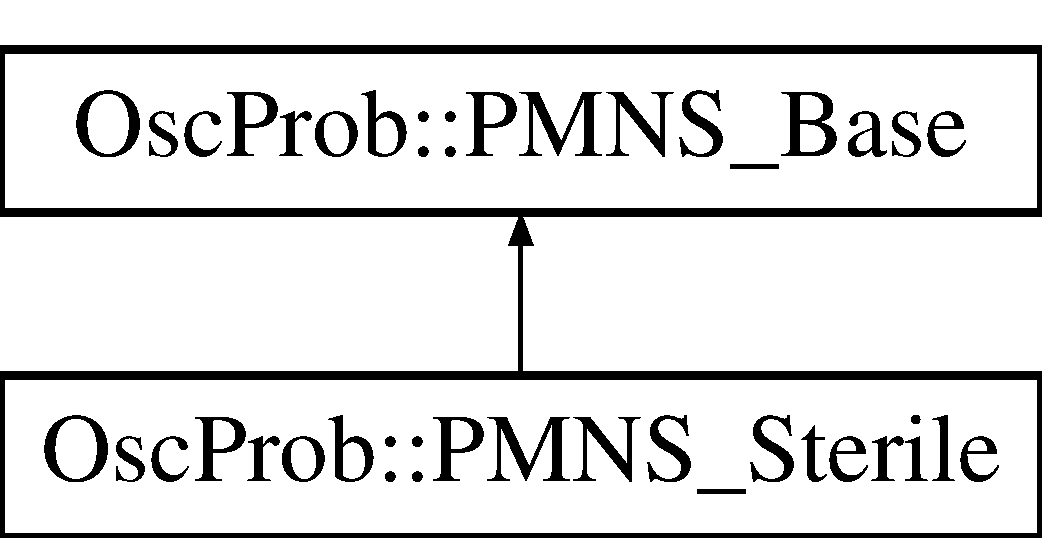
\includegraphics[height=2.000000cm]{classOscProb_1_1PMNS__Sterile}
\end{center}
\end{figure}
\subsection*{Public Member Functions}
\begin{DoxyCompactItemize}
\item 
\hyperlink{classOscProb_1_1PMNS__Sterile_a774766ab4278d9369a295ffa8e2d272c}{P\+M\+N\+S\+\_\+\+Sterile} (int Num\+Nus)
\begin{DoxyCompactList}\small\item\em Constructor. \end{DoxyCompactList}\item 
virtual double \hyperlink{classOscProb_1_1PMNS__Base_aa2e10704d2d205a1ec8988de14b1a66f}{Prob} (std\+::vector$<$ \hyperlink{EigenPoint_8h_a67ca8e107e20610c3fff78d5e726ece0}{complexD} $>$ nu\+\_\+in, int flvf)
\begin{DoxyCompactList}\small\item\em Compute the probability of nu\+\_\+in going to flvf. \end{DoxyCompactList}\item 
virtual double \hyperlink{classOscProb_1_1PMNS__Base_a0190a79284289aacf682c78d7cef9a81}{Prob} (std\+::vector$<$ \hyperlink{EigenPoint_8h_a67ca8e107e20610c3fff78d5e726ece0}{complexD} $>$ nu\+\_\+in, int flvf, double E)
\begin{DoxyCompactList}\small\item\em Compute the probability of nu\+\_\+in going to flvf for energy E. \end{DoxyCompactList}\item 
virtual double \hyperlink{classOscProb_1_1PMNS__Base_a01fba31729345376705e02408e835f67}{Prob} (std\+::vector$<$ \hyperlink{EigenPoint_8h_a67ca8e107e20610c3fff78d5e726ece0}{complexD} $>$ nu\+\_\+in, int flvf, double E, double L)
\begin{DoxyCompactList}\small\item\em Compute the probability of nu\+\_\+in going to flvf for energy E and distance L. \end{DoxyCompactList}\item 
virtual double \hyperlink{classOscProb_1_1PMNS__Base_aec5c399b93261f1962a4b7dbbb44b973}{Prob} (int flvi, int flvf)
\begin{DoxyCompactList}\small\item\em Compute the probability of flvi going to flvf. \end{DoxyCompactList}\item 
virtual double \hyperlink{classOscProb_1_1PMNS__Base_aa3cee10639d5c0879ccb9e78d62128d3}{Prob} (int flvi, int flvf, double E)
\begin{DoxyCompactList}\small\item\em Compute the probability of flvi going to flvf for energy E. \end{DoxyCompactList}\item 
virtual double \hyperlink{classOscProb_1_1PMNS__Base_a6e0a74508d9d6db7be02e242b8467563}{Prob} (int flvi, int flvf, double E, double L)
\begin{DoxyCompactList}\small\item\em Compute the probability of flvi going to flvf for energy E and distance L. \end{DoxyCompactList}\item 
virtual double \hyperlink{classOscProb_1_1PMNS__Base_a89e54c80ae8a31effbab7b2b970606bb}{Avg\+Prob} (std\+::vector$<$ \hyperlink{EigenPoint_8h_a67ca8e107e20610c3fff78d5e726ece0}{complexD} $>$ nu\+\_\+in, int flvf, double E, double dE=0)
\begin{DoxyCompactList}\small\item\em Compute the average probability over a bin of energy. \end{DoxyCompactList}\item 
virtual double \hyperlink{classOscProb_1_1PMNS__Base_ac03f754160422e6600da8dbae0f803ed}{Avg\+Prob} (int flvi, int flvf, double E, double dE=0)
\begin{DoxyCompactList}\small\item\em Compute the average probability over a bin of energy. \end{DoxyCompactList}\item 
virtual double \hyperlink{classOscProb_1_1PMNS__Base_a19f160c045a01e5083506e925fb37d44}{Avg\+Prob\+LoE} (std\+::vector$<$ \hyperlink{EigenPoint_8h_a67ca8e107e20610c3fff78d5e726ece0}{complexD} $>$ nu\+\_\+in, int flvf, double LoE, double d\+LoE=0)
\begin{DoxyCompactList}\small\item\em Compute the average probability over a bin of L/E. \end{DoxyCompactList}\item 
virtual double \hyperlink{classOscProb_1_1PMNS__Base_ac19a92f4ef428a7333ca8eed76fca637}{Avg\+Prob\+LoE} (int flvi, int flvf, double LoE, double d\+LoE=0)
\begin{DoxyCompactList}\small\item\em Compute the average probability over a bin of L/E. \end{DoxyCompactList}\item 
virtual std\+::vector$<$ \hyperlink{EigenPoint_8h_a67ca8e107e20610c3fff78d5e726ece0}{complexD} $>$ \hyperlink{classOscProb_1_1PMNS__Base_a5092561dd8579d390c649eb60803ea98}{Get\+Mass\+Eigenstate} (int mi)
\begin{DoxyCompactList}\small\item\em Get a neutrino mass eigenstate. \end{DoxyCompactList}\item 
virtual void \hyperlink{classOscProb_1_1PMNS__Base_ace7875cf6d3bec161a2b7ed2690aec34}{Set\+Angle} (int i, int j, double th)
\begin{DoxyCompactList}\small\item\em Set the mixing angle theta\+\_\+ij. \end{DoxyCompactList}\item 
virtual void \hyperlink{classOscProb_1_1PMNS__Base_a4bef78cfcfc4e70b4ce79cdb8862c0a3}{Set\+Delta} (int i, int j, double delta)
\begin{DoxyCompactList}\small\item\em Set the CP phase delta\+\_\+ij. \end{DoxyCompactList}\item 
virtual void \hyperlink{classOscProb_1_1PMNS__Base_a492243b22fb1b783cd2943f507cff970}{Set\+Dm} (int j, double dm)
\begin{DoxyCompactList}\small\item\em Set the mass-\/splitting dm\+\_\+j1 in e\+V$^\wedge$2. \end{DoxyCompactList}\item 
virtual double \hyperlink{classOscProb_1_1PMNS__Base_acee137091304c919642293ddf015bbc8}{Get\+Angle} (int i, int j)
\begin{DoxyCompactList}\small\item\em Get the mixing angle theta\+\_\+ij. \end{DoxyCompactList}\item 
virtual double \hyperlink{classOscProb_1_1PMNS__Base_adb8dbc91d4286d2e7c8f768c59476241}{Get\+Delta} (int i, int j)
\begin{DoxyCompactList}\small\item\em Get the CP phase delta\+\_\+ij. \end{DoxyCompactList}\item 
virtual double \hyperlink{classOscProb_1_1PMNS__Base_ad26815ac5f4805d1259817e4936e5f8f}{Get\+Dm} (int j)
\begin{DoxyCompactList}\small\item\em Get the mass-\/splitting dm\+\_\+j1 in e\+V$^\wedge$2. \end{DoxyCompactList}\item 
virtual double \hyperlink{classOscProb_1_1PMNS__Base_a4ea861a6707ce1be3a54aad2b60f8632}{Get\+Dm\+Eff} (int j)
\begin{DoxyCompactList}\small\item\em Get the effective mass-\/splitting dm\+\_\+j1 in e\+V$^\wedge$2. \end{DoxyCompactList}\item 
virtual void \hyperlink{classOscProb_1_1PMNS__Base_a4de96ac9b6d1e9b029ab877e57d211ad}{Set\+Std\+Pars} ()
\begin{DoxyCompactList}\small\item\em Set P\+DG 3-\/flavor parameters. \end{DoxyCompactList}\item 
virtual void \hyperlink{classOscProb_1_1PMNS__Base_a95b3b0d0cab5e6a54b5ef99587f837c0}{Set\+Energy} (double E)
\begin{DoxyCompactList}\small\item\em Set the neutrino energy in GeV. \end{DoxyCompactList}\item 
virtual void \hyperlink{classOscProb_1_1PMNS__Base_a717e0348cf762f3961854e332a9b52e0}{Set\+Is\+Nu\+Bar} (bool is\+Nu\+Bar)
\begin{DoxyCompactList}\small\item\em Set the anti-\/neutrino flag. \end{DoxyCompactList}\item 
virtual double \hyperlink{classOscProb_1_1PMNS__Base_acc0d46cc4b8f911b40b807225003bbed}{Get\+Energy} ()
\begin{DoxyCompactList}\small\item\em Get the neutrino energy in GeV. \end{DoxyCompactList}\item 
virtual bool \hyperlink{classOscProb_1_1PMNS__Base_a2f7f2a028dfe7a90fff6b4f757972c2c}{Get\+Is\+Nu\+Bar} ()
\begin{DoxyCompactList}\small\item\em Get the anti-\/neutrino flag. \end{DoxyCompactList}\item 
virtual void \hyperlink{classOscProb_1_1PMNS__Base_ac3b644fd0a56347d304ceca4ae9d8875}{Set\+Path} (\hyperlink{structOscProb_1_1NuPath}{Osc\+Prob\+::\+Nu\+Path} p)
\begin{DoxyCompactList}\small\item\em Set a single path. \end{DoxyCompactList}\item 
virtual void \hyperlink{classOscProb_1_1PMNS__Base_a35b983270613072a3df58b574d80dbfd}{Set\+Path} (double length, double density, double zoa=0.\+5, int layer=0)
\begin{DoxyCompactList}\small\item\em Set a single path. \end{DoxyCompactList}\item 
virtual void \hyperlink{classOscProb_1_1PMNS__Base_a637d19dd850b4246507796526622643c}{Set\+Path} (std\+::vector$<$ \hyperlink{structOscProb_1_1NuPath}{Osc\+Prob\+::\+Nu\+Path} $>$ paths)
\begin{DoxyCompactList}\small\item\em Set a path sequence. \end{DoxyCompactList}\item 
virtual void \hyperlink{classOscProb_1_1PMNS__Base_a887dc9d4dc569ec0cdef3933b4c60efc}{Add\+Path} (\hyperlink{structOscProb_1_1NuPath}{Osc\+Prob\+::\+Nu\+Path} p)
\begin{DoxyCompactList}\small\item\em Add a path to the sequence. \end{DoxyCompactList}\item 
virtual void \hyperlink{classOscProb_1_1PMNS__Base_ab7f89ad9e7e1224adaa59d3c41594cd9}{Add\+Path} (double length, double density, double zoa=0.\+5, int layer=0)
\begin{DoxyCompactList}\small\item\em Add a path to the sequence. \end{DoxyCompactList}\item 
virtual void \hyperlink{classOscProb_1_1PMNS__Base_aefe521239031c418cfaaaa550a6e13bb}{Clear\+Path} ()
\begin{DoxyCompactList}\small\item\em Clear the path vector. \end{DoxyCompactList}\item 
virtual void \hyperlink{classOscProb_1_1PMNS__Base_a6241325b1bd28cafa556daaecbe4ed62}{Set\+Length} (double L)
\begin{DoxyCompactList}\small\item\em Set a single path lentgh in km. \end{DoxyCompactList}\item 
virtual void \hyperlink{classOscProb_1_1PMNS__Base_aa34a40a3b5abda0f252982d9ead3b520}{Set\+Length} (std\+::vector$<$ double $>$ L)
\begin{DoxyCompactList}\small\item\em Set multiple path lengths. \end{DoxyCompactList}\item 
virtual void \hyperlink{classOscProb_1_1PMNS__Base_ac74206f349687da141392c81e2ba6b0d}{Set\+Density} (double rho)
\begin{DoxyCompactList}\small\item\em Set single path density in g/cm$^\wedge$3. \end{DoxyCompactList}\item 
virtual void \hyperlink{classOscProb_1_1PMNS__Base_a858221d5510fe732dc6a101fd305cda0}{Set\+Density} (std\+::vector$<$ double $>$ rho)
\begin{DoxyCompactList}\small\item\em Set multiple path densities. \end{DoxyCompactList}\item 
virtual void \hyperlink{classOscProb_1_1PMNS__Base_a1bf3ea8fd2507fd2fd82d7410ff8f578}{Set\+ZoA} (double zoa)
\begin{DoxyCompactList}\small\item\em Set Z/A value for single path. \end{DoxyCompactList}\item 
virtual void \hyperlink{classOscProb_1_1PMNS__Base_a8495f8a320e1a21965e6a64aec92ad2a}{Set\+ZoA} (std\+::vector$<$ double $>$ zoa)
\begin{DoxyCompactList}\small\item\em Set multiple path Z/A values. \end{DoxyCompactList}\item 
virtual void \hyperlink{classOscProb_1_1PMNS__Base_a904e580edf89fb98bf9a6397739b4ebe}{Set\+Layers} (std\+::vector$<$ int $>$ lay)
\begin{DoxyCompactList}\small\item\em Set multiple path layer indices. \end{DoxyCompactList}\item 
virtual void \hyperlink{classOscProb_1_1PMNS__Base_add6533a9fc9acdfc7ae258b62570d78d}{Set\+Std\+Path} ()
\begin{DoxyCompactList}\small\item\em Set standard neutrino path. \end{DoxyCompactList}\item 
virtual std\+::vector$<$ \hyperlink{structOscProb_1_1NuPath}{Osc\+Prob\+::\+Nu\+Path} $>$ \hyperlink{classOscProb_1_1PMNS__Base_ac8e196f2e85a2b1caaf705073ee95a5c}{Get\+Path} ()
\begin{DoxyCompactList}\small\item\em Get the neutrino path sequence. \end{DoxyCompactList}\item 
virtual std\+::vector$<$ double $>$ \hyperlink{classOscProb_1_1PMNS__Base_a9eac8d768c1424755ee41f7e783af179}{Get\+Sample\+Points} (double LoE, double d\+LoE)
\begin{DoxyCompactList}\small\item\em Compute the sample points for a bin of L/E with width d\+LoE. \end{DoxyCompactList}\item 
virtual void \hyperlink{classOscProb_1_1PMNS__Base_aa94c1e1fff0ba731c75f7e633b023a9f}{Set\+Use\+Cache} (bool u=true)
\begin{DoxyCompactList}\small\item\em Set caching on/off. \end{DoxyCompactList}\item 
virtual void \hyperlink{classOscProb_1_1PMNS__Base_ac47fd33e69aa6490f99e2fd147a92f03}{Clear\+Cache} ()
\begin{DoxyCompactList}\small\item\em Clear the cache. \end{DoxyCompactList}\item 
virtual void \hyperlink{classOscProb_1_1PMNS__Base_ae67862cf58b0802487a14b047b012a78}{Set\+Max\+Cache} (int mc=1e6)
\begin{DoxyCompactList}\small\item\em Set max cache size. \end{DoxyCompactList}\end{DoxyCompactItemize}
\subsection*{Protected Member Functions}
\begin{DoxyCompactItemize}
\item 
virtual void \hyperlink{classOscProb_1_1PMNS__Sterile_af60f89862d0fe333c62d6f87ecfd89f8}{Solve\+Ham} ()
\begin{DoxyCompactList}\small\item\em Solve the full Hamiltonian for eigenvectors and eigenvalues. \end{DoxyCompactList}\item 
virtual void \hyperlink{classOscProb_1_1PMNS__Base_adf23b569112f9f9e0e592f01d79a5f3d}{Initialize\+Vectors} ()
\begin{DoxyCompactList}\small\item\em Initialize all member vectors with zeros. \end{DoxyCompactList}\item 
virtual bool \hyperlink{classOscProb_1_1PMNS__Base_abe533da5f64bec1f4724ab7b58606b77}{Try\+Cache} ()
\begin{DoxyCompactList}\small\item\em Try to find a cached eigensystem. \end{DoxyCompactList}\item 
virtual void \hyperlink{classOscProb_1_1PMNS__Base_a785c37fcea974628623c8881bb0fbbf9}{Fill\+Cache} ()
\begin{DoxyCompactList}\small\item\em Cache the current eigensystem. \end{DoxyCompactList}\item 
virtual void \hyperlink{classOscProb_1_1PMNS__Base_a986e6ebef09a7e2eb7fee16a4c2c834d}{Set\+Cur\+Path} (\hyperlink{structOscProb_1_1NuPath}{Osc\+Prob\+::\+Nu\+Path} p)
\begin{DoxyCompactList}\small\item\em Set the path currently in use by the class. \end{DoxyCompactList}\item 
virtual void \hyperlink{classOscProb_1_1PMNS__Base_aba565962a440d14bee7a2a96d2eca2c5}{Set\+Att} (double att, int idx)
\begin{DoxyCompactList}\small\item\em Set one of the path attributes. \end{DoxyCompactList}\item 
virtual void \hyperlink{classOscProb_1_1PMNS__Base_aa001479b5f5828c3d16ed087f96ecbcc}{Set\+Att} (std\+::vector$<$ double $>$ att, int idx)
\begin{DoxyCompactList}\small\item\em Set all values of a path attribute. \end{DoxyCompactList}\item 
virtual void \hyperlink{classOscProb_1_1PMNS__Base_a6a3cf45bbe2349abf06708b65677c044}{RotateH} (int i, int j, std\+::vector$<$ std\+::vector$<$ \hyperlink{EigenPoint_8h_a67ca8e107e20610c3fff78d5e726ece0}{complexD} $>$ $>$ \&Ham)
\begin{DoxyCompactList}\small\item\em Rotate the Hamiltonian by theta\+\_\+ij and delta\+\_\+ij. \end{DoxyCompactList}\item 
virtual void \hyperlink{classOscProb_1_1PMNS__Base_ae52554477ad3250daa5adb8c32cab0b4}{Rotate\+State} (int i, int j)
\begin{DoxyCompactList}\small\item\em Rotate the neutrino state by theta\+\_\+ij and delta\+\_\+ij. \end{DoxyCompactList}\item 
virtual void \hyperlink{classOscProb_1_1PMNS__Base_ad0faf5eae755afb1baa1fcd5ffebad41}{Build\+Hms} ()
\begin{DoxyCompactList}\small\item\em Build the matrix of masses squared. \end{DoxyCompactList}\item 
virtual void \hyperlink{classOscProb_1_1PMNS__Base_ac0d4bf8ff1318ef96d3dafa62e0cec25}{Reset\+To\+Flavour} (int flv)
\begin{DoxyCompactList}\small\item\em Reset neutrino state to pure flavour flv. \end{DoxyCompactList}\item 
virtual void \hyperlink{classOscProb_1_1PMNS__Base_accb08503acc162188041d7a96a280462}{Propagate\+Path} (\hyperlink{structOscProb_1_1NuPath}{Osc\+Prob\+::\+Nu\+Path} p)
\begin{DoxyCompactList}\small\item\em Propagate neutrino through a single path. \end{DoxyCompactList}\item 
virtual void \hyperlink{classOscProb_1_1PMNS__Base_a054e3a8b05b9a958b6fa416e4a835e3e}{Propagate} ()
\begin{DoxyCompactList}\small\item\em Propagate neutrino through full path. \end{DoxyCompactList}\item 
virtual double \hyperlink{classOscProb_1_1PMNS__Base_a0dc4d45bc3d7e03b9abbf5b4e100cc22}{P} (int flv)
\begin{DoxyCompactList}\small\item\em Return the probability of final state in flavour flv. \end{DoxyCompactList}\end{DoxyCompactItemize}
\subsection*{Protected Attributes}
\begin{DoxyCompactItemize}
\item 
\hyperlink{structOscProb_1_1GSL__EinSys}{G\+S\+L\+\_\+\+Ein\+Sys} \hyperlink{classOscProb_1_1PMNS__Sterile_a92e9493bcec35167cef6cc472d178449}{f\+G\+SL}
\item 
int \hyperlink{classOscProb_1_1PMNS__Base_a24bb74bed63569dfe88b18fa6a08060e}{f\+Num\+Nus}
\begin{DoxyCompactList}\small\item\em Number of neutrino flavours. \end{DoxyCompactList}\item 
std\+::vector$<$ double $>$ \hyperlink{classOscProb_1_1PMNS__Base_a406a31c3b5d620e5a0cace5b411f9f70}{f\+Dm}
\begin{DoxyCompactList}\small\item\em m$^\wedge$2\+\_\+i -\/ m$^\wedge$2\+\_\+1 in vacuum \end{DoxyCompactList}\item 
std\+::vector$<$ std\+::vector$<$ double $>$ $>$ \hyperlink{classOscProb_1_1PMNS__Base_a1976887cd658dd86b2336c181f1470b4}{f\+Theta}
\begin{DoxyCompactList}\small\item\em theta\mbox{[}i\mbox{]}\mbox{[}j\mbox{]} mixing angle \end{DoxyCompactList}\item 
std\+::vector$<$ std\+::vector$<$ double $>$ $>$ \hyperlink{classOscProb_1_1PMNS__Base_ab2a5fa40e689b221c8a7d2c17213810d}{f\+Delta}
\begin{DoxyCompactList}\small\item\em delta\mbox{[}i\mbox{]}\mbox{[}j\mbox{]} CP violating phase \end{DoxyCompactList}\item 
std\+::vector$<$ \hyperlink{EigenPoint_8h_a67ca8e107e20610c3fff78d5e726ece0}{complexD} $>$ \hyperlink{classOscProb_1_1PMNS__Base_abf99f2339e3ee989600740b5d88063e8}{f\+Nu\+State}
\begin{DoxyCompactList}\small\item\em The neutrino current state. \end{DoxyCompactList}\item 
std\+::vector$<$ std\+::vector$<$ \hyperlink{EigenPoint_8h_a67ca8e107e20610c3fff78d5e726ece0}{complexD} $>$ $>$ \hyperlink{classOscProb_1_1PMNS__Base_acd3c8783e7603081eab316ea4c86c766}{f\+Hms}
\begin{DoxyCompactList}\small\item\em matrix H$\ast$2E in e\+V$^\wedge$2 \end{DoxyCompactList}\item 
std\+::vector$<$ \hyperlink{EigenPoint_8h_a67ca8e107e20610c3fff78d5e726ece0}{complexD} $>$ \hyperlink{classOscProb_1_1PMNS__Base_ab8d26b722047d49d977f5f2d83026ede}{f\+Phases}
\begin{DoxyCompactList}\small\item\em Buffer for oscillation phases. \end{DoxyCompactList}\item 
std\+::vector$<$ \hyperlink{EigenPoint_8h_a67ca8e107e20610c3fff78d5e726ece0}{complexD} $>$ \hyperlink{classOscProb_1_1PMNS__Base_a5440bc3efa466a37649601abce559e3e}{f\+Buffer}
\begin{DoxyCompactList}\small\item\em Buffer for neutrino state tranformations. \end{DoxyCompactList}\item 
std\+::vector$<$ double $>$ \hyperlink{classOscProb_1_1PMNS__Base_a6319c34d7decbb9d7d6da279c06e8c2d}{f\+Eval}
\begin{DoxyCompactList}\small\item\em Eigenvalues of the Hamiltonian. \end{DoxyCompactList}\item 
std\+::vector$<$ std\+::vector$<$ \hyperlink{EigenPoint_8h_a67ca8e107e20610c3fff78d5e726ece0}{complexD} $>$ $>$ \hyperlink{classOscProb_1_1PMNS__Base_a87be137356c5f27ab83cab5e1298ef8f}{f\+Evec}
\begin{DoxyCompactList}\small\item\em Eigenvectors of the Hamiltonian. \end{DoxyCompactList}\item 
double \hyperlink{classOscProb_1_1PMNS__Base_a2800af6d436972f3e900867790c046b0}{f\+Energy}
\begin{DoxyCompactList}\small\item\em Neutrino energy. \end{DoxyCompactList}\item 
bool \hyperlink{classOscProb_1_1PMNS__Base_a0ebaeaefab36a3ff381c6293faedfdd6}{f\+Is\+Nu\+Bar}
\begin{DoxyCompactList}\small\item\em Anti-\/neutrino flag. \end{DoxyCompactList}\item 
std\+::vector$<$ \hyperlink{structOscProb_1_1NuPath}{Osc\+Prob\+::\+Nu\+Path} $>$ \hyperlink{classOscProb_1_1PMNS__Base_a69db9d57e12fc7cbe0431bc6c18fac93}{f\+Nu\+Paths}
\begin{DoxyCompactList}\small\item\em Vector of neutrino paths. \end{DoxyCompactList}\item 
\hyperlink{structOscProb_1_1NuPath}{Osc\+Prob\+::\+Nu\+Path} \hyperlink{classOscProb_1_1PMNS__Base_a849437aa8891fe042e86886ce8f81c6e}{f\+Path}
\begin{DoxyCompactList}\small\item\em Current neutrino path. \end{DoxyCompactList}\item 
bool \hyperlink{classOscProb_1_1PMNS__Base_a9ac3cadeac8db1b90f3152f476244780}{f\+Built\+Hms}
\begin{DoxyCompactList}\small\item\em Tag to avoid rebuilding Hms. \end{DoxyCompactList}\item 
bool \hyperlink{classOscProb_1_1PMNS__Base_a6dc5cd010d2d70b2324745b4e53e9839}{f\+Got\+ES}
\begin{DoxyCompactList}\small\item\em Tag to avoid recalculating eigensystem. \end{DoxyCompactList}\item 
bool \hyperlink{classOscProb_1_1PMNS__Base_ad28c12ef897b5555eda509ea55c99107}{f\+Use\+Cache}
\begin{DoxyCompactList}\small\item\em Flag for whether to use caching. \end{DoxyCompactList}\item 
double \hyperlink{classOscProb_1_1PMNS__Base_a0b4c41a27de281472453a1912cbc1e64}{f\+Cache\+Prec}
\begin{DoxyCompactList}\small\item\em Precision of cache matching. \end{DoxyCompactList}\item 
int \hyperlink{classOscProb_1_1PMNS__Base_a74c13356eafec2490d8c3c19759ba7f0}{f\+Max\+Cache}
\begin{DoxyCompactList}\small\item\em Maximum cache size. \end{DoxyCompactList}\item 
std\+::set$<$ \hyperlink{structOscProb_1_1EigenPoint}{Osc\+Prob\+::\+Eigen\+Point} $>$ \hyperlink{classOscProb_1_1PMNS__Base_a8159424f20197a3a7145fe3bf2c11176}{f\+Mix\+Cache}
\begin{DoxyCompactList}\small\item\em Caching set of eigensystems. \end{DoxyCompactList}\item 
\hyperlink{structOscProb_1_1EigenPoint}{Eigen\+Point} \hyperlink{classOscProb_1_1PMNS__Base_ab1fe4800ee3ae48df4fc942dce00e0d3}{f\+Probe}
\begin{DoxyCompactList}\small\item\em Eigenp\+Point to try. \end{DoxyCompactList}\end{DoxyCompactItemize}
\subsection*{Static Protected Attributes}
\begin{DoxyCompactItemize}
\item 
static const \hyperlink{EigenPoint_8h_a67ca8e107e20610c3fff78d5e726ece0}{complexD} \hyperlink{classOscProb_1_1PMNS__Base_a05e595848c2521dc795efa7645728b94}{zero}
\begin{DoxyCompactList}\small\item\em zero in complex \end{DoxyCompactList}\item 
static const \hyperlink{EigenPoint_8h_a67ca8e107e20610c3fff78d5e726ece0}{complexD} \hyperlink{classOscProb_1_1PMNS__Base_a7d1d0bbcab30a1fd8c368c40134c51ff}{one}
\begin{DoxyCompactList}\small\item\em one in complex \end{DoxyCompactList}\item 
static const double \hyperlink{classOscProb_1_1PMNS__Base_a382ddd7b76ca89b43f22614a2ea7327b}{k\+Km2eV} = 1.\+0 / 1.\+973269788e-\/10
\begin{DoxyCompactList}\small\item\em km to e\+V$^\wedge$-\/1 \end{DoxyCompactList}\item 
static const double \hyperlink{classOscProb_1_1PMNS__Base_a326fc5016d7dd7ce05682c06cdcb6d94}{k\+K2} = 1e-\/3 $\ast$ k\+N\+A / pow(k\+Km2e\+V,3)
\begin{DoxyCompactList}\small\item\em mol/\+Ge\+V$^\wedge$2/cm$^\wedge$3 to eV \end{DoxyCompactList}\item 
static const double \hyperlink{classOscProb_1_1PMNS__Base_ad36a0a6bf58d6ec093d3947784bd89e9}{k\+Ge\+V2eV} = 1.\+0e+09
\begin{DoxyCompactList}\small\item\em GeV to eV. \end{DoxyCompactList}\item 
static const double \hyperlink{classOscProb_1_1PMNS__Base_a69355e770b89e99437c2b8a66e48eeb9}{k\+NA} = 6.\+022140857e23
\begin{DoxyCompactList}\small\item\em Avogadro constant. \end{DoxyCompactList}\item 
static const double \hyperlink{classOscProb_1_1PMNS__Base_a7f26a3456128234b2ae6cc9141a6532f}{k\+Gf} = 1.\+1663787e-\/05
\begin{DoxyCompactList}\small\item\em G\+\_\+F in units of Ge\+V$^\wedge$-\/2. \end{DoxyCompactList}\end{DoxyCompactItemize}


\subsection{Detailed Description}
This class implements neutrino oscillations for any number of neutrino falvours. The extra flavours above 3 are treated as sterile neutrinos, i.\+e. it implements a 3+N model. One can also run a 2-\/neutrino model in principle, but an analytical solution would be feasible and more efficient in that case.

The eigensystem solution is performed by G\+SL, which makes it slower than the \hyperlink{classOscProb_1_1PMNS__Fast}{P\+M\+N\+S\+\_\+\+Fast} class, which only works for 3 neutrinos.

\begin{DoxyAuthor}{Author}
coelho@lal.\+in2p3.\+fr 
\end{DoxyAuthor}


Definition at line 43 of file P\+M\+N\+S\+\_\+\+Sterile.\+h.



\subsection{Constructor \& Destructor Documentation}
\mbox{\Hypertarget{classOscProb_1_1PMNS__Sterile_a774766ab4278d9369a295ffa8e2d272c}\label{classOscProb_1_1PMNS__Sterile_a774766ab4278d9369a295ffa8e2d272c}} 
\index{Osc\+Prob\+::\+P\+M\+N\+S\+\_\+\+Sterile@{Osc\+Prob\+::\+P\+M\+N\+S\+\_\+\+Sterile}!P\+M\+N\+S\+\_\+\+Sterile@{P\+M\+N\+S\+\_\+\+Sterile}}
\index{P\+M\+N\+S\+\_\+\+Sterile@{P\+M\+N\+S\+\_\+\+Sterile}!Osc\+Prob\+::\+P\+M\+N\+S\+\_\+\+Sterile@{Osc\+Prob\+::\+P\+M\+N\+S\+\_\+\+Sterile}}
\subsubsection{\texorpdfstring{P\+M\+N\+S\+\_\+\+Sterile()}{PMNS\_Sterile()}}
{\footnotesize\ttfamily P\+M\+N\+S\+\_\+\+Sterile\+::\+P\+M\+N\+S\+\_\+\+Sterile (\begin{DoxyParamCaption}\item[{int}]{num\+Nus }\end{DoxyParamCaption})}

Constructor. \begin{DoxySeeAlso}{See also}
\hyperlink{classOscProb_1_1PMNS__Base_aa53e83b03a9cf4bdfa0a07136bd17a79}{P\+M\+N\+S\+\_\+\+Base\+::\+P\+M\+N\+S\+\_\+\+Base}
\end{DoxySeeAlso}
This class can implement any number of neutrino flavours.


\begin{DoxyParams}{Parameters}
{\em num\+Nus} & -\/ the number of neutrino flavours \\
\hline
\end{DoxyParams}


Definition at line 135 of file P\+M\+N\+S\+\_\+\+Sterile.\+cxx.


\begin{DoxyCode}
135                                      :
136 \hyperlink{classOscProb_1_1PMNS__Base_aa53e83b03a9cf4bdfa0a07136bd17a79}{PMNS\_Base}(numNus), \hyperlink{classOscProb_1_1PMNS__Sterile_a92e9493bcec35167cef6cc472d178449}{fGSL}(numNus) \{\}
\end{DoxyCode}


\subsection{Member Function Documentation}
\mbox{\Hypertarget{classOscProb_1_1PMNS__Base_a887dc9d4dc569ec0cdef3933b4c60efc}\label{classOscProb_1_1PMNS__Base_a887dc9d4dc569ec0cdef3933b4c60efc}} 
\index{Osc\+Prob\+::\+P\+M\+N\+S\+\_\+\+Sterile@{Osc\+Prob\+::\+P\+M\+N\+S\+\_\+\+Sterile}!Add\+Path@{Add\+Path}}
\index{Add\+Path@{Add\+Path}!Osc\+Prob\+::\+P\+M\+N\+S\+\_\+\+Sterile@{Osc\+Prob\+::\+P\+M\+N\+S\+\_\+\+Sterile}}
\subsubsection{\texorpdfstring{Add\+Path()}{AddPath()}\hspace{0.1cm}{\footnotesize\ttfamily [1/2]}}
{\footnotesize\ttfamily void P\+M\+N\+S\+\_\+\+Base\+::\+Add\+Path (\begin{DoxyParamCaption}\item[{\hyperlink{structOscProb_1_1NuPath}{Osc\+Prob\+::\+Nu\+Path}}]{p }\end{DoxyParamCaption})\hspace{0.3cm}{\ttfamily [virtual]}, {\ttfamily [inherited]}}

Add a path to the sequence. 
\begin{DoxyParams}{Parameters}
{\em p} & -\/ A neutrino path segment \\
\hline
\end{DoxyParams}


Definition at line 351 of file P\+M\+N\+S\+\_\+\+Base.\+cxx.



References Osc\+Prob\+::\+P\+M\+N\+S\+\_\+\+Base\+::f\+Nu\+Paths.



Referenced by Osc\+Prob\+::\+P\+M\+N\+S\+\_\+\+Base\+::\+Add\+Path(), Osc\+Prob\+::\+P\+M\+N\+S\+\_\+\+Base\+::\+Set\+Att(), and Osc\+Prob\+::\+P\+M\+N\+S\+\_\+\+Base\+::\+Set\+Path().


\begin{DoxyCode}
351                                \{
352 
353   \hyperlink{classOscProb_1_1PMNS__Base_a69db9d57e12fc7cbe0431bc6c18fac93}{fNuPaths}.push\_back(p);
354 
355 \}
\end{DoxyCode}
\mbox{\Hypertarget{classOscProb_1_1PMNS__Base_ab7f89ad9e7e1224adaa59d3c41594cd9}\label{classOscProb_1_1PMNS__Base_ab7f89ad9e7e1224adaa59d3c41594cd9}} 
\index{Osc\+Prob\+::\+P\+M\+N\+S\+\_\+\+Sterile@{Osc\+Prob\+::\+P\+M\+N\+S\+\_\+\+Sterile}!Add\+Path@{Add\+Path}}
\index{Add\+Path@{Add\+Path}!Osc\+Prob\+::\+P\+M\+N\+S\+\_\+\+Sterile@{Osc\+Prob\+::\+P\+M\+N\+S\+\_\+\+Sterile}}
\subsubsection{\texorpdfstring{Add\+Path()}{AddPath()}\hspace{0.1cm}{\footnotesize\ttfamily [2/2]}}
{\footnotesize\ttfamily void P\+M\+N\+S\+\_\+\+Base\+::\+Add\+Path (\begin{DoxyParamCaption}\item[{double}]{length,  }\item[{double}]{density,  }\item[{double}]{zoa = {\ttfamily 0.5},  }\item[{int}]{layer = {\ttfamily 0} }\end{DoxyParamCaption})\hspace{0.3cm}{\ttfamily [virtual]}, {\ttfamily [inherited]}}

Add a path to the sequence defining attributes directly. 
\begin{DoxyParams}{Parameters}
{\em length} & -\/ The length of the path segment in km \\
\hline
{\em density} & -\/ The density of the path segment in g/cm$^\wedge$3 \\
\hline
{\em zoa} & -\/ The effective Z/A of the path segment \\
\hline
{\em layer} & -\/ An index to identify the layer type (e.\+g. earth inner core) \\
\hline
\end{DoxyParams}


Definition at line 365 of file P\+M\+N\+S\+\_\+\+Base.\+cxx.



References Osc\+Prob\+::\+P\+M\+N\+S\+\_\+\+Base\+::\+Add\+Path().


\begin{DoxyCode}
365                                                                            \{
366 
367   \hyperlink{classOscProb_1_1PMNS__Base_a887dc9d4dc569ec0cdef3933b4c60efc}{AddPath}(\hyperlink{structOscProb_1_1NuPath}{NuPath}(length, density, zoa, layer));
368 
369 \}
\end{DoxyCode}
\mbox{\Hypertarget{classOscProb_1_1PMNS__Base_a89e54c80ae8a31effbab7b2b970606bb}\label{classOscProb_1_1PMNS__Base_a89e54c80ae8a31effbab7b2b970606bb}} 
\index{Osc\+Prob\+::\+P\+M\+N\+S\+\_\+\+Sterile@{Osc\+Prob\+::\+P\+M\+N\+S\+\_\+\+Sterile}!Avg\+Prob@{Avg\+Prob}}
\index{Avg\+Prob@{Avg\+Prob}!Osc\+Prob\+::\+P\+M\+N\+S\+\_\+\+Sterile@{Osc\+Prob\+::\+P\+M\+N\+S\+\_\+\+Sterile}}
\subsubsection{\texorpdfstring{Avg\+Prob()}{AvgProb()}\hspace{0.1cm}{\footnotesize\ttfamily [1/2]}}
{\footnotesize\ttfamily double P\+M\+N\+S\+\_\+\+Base\+::\+Avg\+Prob (\begin{DoxyParamCaption}\item[{std\+::vector$<$ \hyperlink{EigenPoint_8h_a67ca8e107e20610c3fff78d5e726ece0}{complexD} $>$}]{nu\+\_\+in,  }\item[{int}]{flvf,  }\item[{double}]{E,  }\item[{double}]{dE = {\ttfamily 0} }\end{DoxyParamCaption})\hspace{0.3cm}{\ttfamily [virtual]}, {\ttfamily [inherited]}}

Compute the average probability of nu\+\_\+in going to flvf over a bin of energy E with width dE.

This gets transformed into L/E, since the oscillation terms have arguments linear in L/E and not E.

This function works best for single paths. In multiple paths the accuracy may be somewhat worse. If needed, average over smaller energy ranges.

Flavours are\+: 
\begin{DoxyPre}
  0 = nue, 1 = numu, 2 = nutau
  3 = sterile\_1, 4 = sterile\_2, etc.
\end{DoxyPre}
 
\begin{DoxyParams}{Parameters}
{\em nu\+\_\+in} & -\/ The neutrino initial state in flavour. \\
\hline
{\em flvf} & -\/ The neutrino final flavour. \\
\hline
{\em E} & -\/ The neutrino energy in the bin center in GeV \\
\hline
{\em dE} & -\/ The energy bin width in GeV\\
\hline
\end{DoxyParams}
\begin{DoxyReturn}{Returns}
Average neutrino oscillation probability 
\end{DoxyReturn}


Definition at line 1386 of file P\+M\+N\+S\+\_\+\+Base.\+cxx.



References Osc\+Prob\+::\+Avg\+Path(), Osc\+Prob\+::\+P\+M\+N\+S\+\_\+\+Base\+::\+Avg\+Prob\+Lo\+E(), Osc\+Prob\+::\+P\+M\+N\+S\+\_\+\+Base\+::f\+Nu\+Paths, Osc\+Prob\+::\+P\+M\+N\+S\+\_\+\+Base\+::f\+Path, Osc\+Prob\+::\+Nu\+Path\+::length, Osc\+Prob\+::\+P\+M\+N\+S\+\_\+\+Base\+::\+Prob(), and Osc\+Prob\+::\+P\+M\+N\+S\+\_\+\+Base\+::\+Set\+Cur\+Path().



Referenced by Osc\+Prob\+::\+P\+M\+N\+S\+\_\+\+Base\+::\+Avg\+Prob().


\begin{DoxyCode}
1387 \{
1388 
1389   \textcolor{comment}{// Do nothing if energy is not positive}
1390   \textcolor{keywordflow}{if}(E<=0) \textcolor{keywordflow}{return} 0;
1391 
1392   \textcolor{keywordflow}{if}(\hyperlink{classOscProb_1_1PMNS__Base_a69db9d57e12fc7cbe0431bc6c18fac93}{fNuPaths}.empty()) \textcolor{keywordflow}{return} 0;
1393 
1394   \textcolor{comment}{// Don't average zero width}
1395   \textcolor{keywordflow}{if}(dE<=0) \textcolor{keywordflow}{return} \hyperlink{classOscProb_1_1PMNS__Base_aa2e10704d2d205a1ec8988de14b1a66f}{Prob}(nu\_in, flvf, E);
1396 
1397   \textcolor{comment}{// Make sure fPath is set}
1398   \textcolor{comment}{// Use average if multiple paths}
1399   \hyperlink{classOscProb_1_1PMNS__Base_a986e6ebef09a7e2eb7fee16a4c2c834d}{SetCurPath}(\hyperlink{namespaceOscProb_a999a7944bad8bc72d7ee9f56f81a210e}{AvgPath}(\hyperlink{classOscProb_1_1PMNS__Base_a69db9d57e12fc7cbe0431bc6c18fac93}{fNuPaths}));
1400 
1401   \textcolor{comment}{// Define L/E variables}
1402   \textcolor{keywordtype}{double} LoE = 0;
1403   \textcolor{keywordtype}{double} dLoE = 0;
1404 
1405   \textcolor{comment}{// Set a minimum energy}
1406   \textcolor{keywordtype}{double} minE = 0.1 * E;
1407 
1408   \textcolor{comment}{// Transform range to L/E}
1409   \textcolor{comment}{// Full range if low edge > minE}
1410   \textcolor{keywordflow}{if}(E-dE/2 > minE)\{
1411     LoE = 0.5 * (\hyperlink{classOscProb_1_1PMNS__Base_a849437aa8891fe042e86886ce8f81c6e}{fPath}.\hyperlink{structOscProb_1_1NuPath_af22660894b6e25cf835500381b155557}{length}/(E-dE/2) + \hyperlink{classOscProb_1_1PMNS__Base_a849437aa8891fe042e86886ce8f81c6e}{fPath}.\hyperlink{structOscProb_1_1NuPath_af22660894b6e25cf835500381b155557}{length}/(E+dE/2));
1412     dLoE = \hyperlink{classOscProb_1_1PMNS__Base_a849437aa8891fe042e86886ce8f81c6e}{fPath}.\hyperlink{structOscProb_1_1NuPath_af22660894b6e25cf835500381b155557}{length}/(E-dE/2) - \hyperlink{classOscProb_1_1PMNS__Base_a849437aa8891fe042e86886ce8f81c6e}{fPath}.\hyperlink{structOscProb_1_1NuPath_af22660894b6e25cf835500381b155557}{length}/(E+dE/2);
1413   \}
1414   \textcolor{comment}{// Else start at minE}
1415   \textcolor{keywordflow}{else}\{
1416     LoE = 0.5 * (\hyperlink{classOscProb_1_1PMNS__Base_a849437aa8891fe042e86886ce8f81c6e}{fPath}.\hyperlink{structOscProb_1_1NuPath_af22660894b6e25cf835500381b155557}{length}/minE + \hyperlink{classOscProb_1_1PMNS__Base_a849437aa8891fe042e86886ce8f81c6e}{fPath}.\hyperlink{structOscProb_1_1NuPath_af22660894b6e25cf835500381b155557}{length}/(E+dE/2));
1417     dLoE = \hyperlink{classOscProb_1_1PMNS__Base_a849437aa8891fe042e86886ce8f81c6e}{fPath}.\hyperlink{structOscProb_1_1NuPath_af22660894b6e25cf835500381b155557}{length}/minE - \hyperlink{classOscProb_1_1PMNS__Base_a849437aa8891fe042e86886ce8f81c6e}{fPath}.\hyperlink{structOscProb_1_1NuPath_af22660894b6e25cf835500381b155557}{length}/(E+dE/2);
1418   \}
1419 
1420   \textcolor{comment}{// Compute average in LoE}
1421   \textcolor{keywordflow}{return} \hyperlink{classOscProb_1_1PMNS__Base_a19f160c045a01e5083506e925fb37d44}{AvgProbLoE}(nu\_in, flvf, LoE, dLoE);
1422 
1423 \}
\end{DoxyCode}
\mbox{\Hypertarget{classOscProb_1_1PMNS__Base_ac03f754160422e6600da8dbae0f803ed}\label{classOscProb_1_1PMNS__Base_ac03f754160422e6600da8dbae0f803ed}} 
\index{Osc\+Prob\+::\+P\+M\+N\+S\+\_\+\+Sterile@{Osc\+Prob\+::\+P\+M\+N\+S\+\_\+\+Sterile}!Avg\+Prob@{Avg\+Prob}}
\index{Avg\+Prob@{Avg\+Prob}!Osc\+Prob\+::\+P\+M\+N\+S\+\_\+\+Sterile@{Osc\+Prob\+::\+P\+M\+N\+S\+\_\+\+Sterile}}
\subsubsection{\texorpdfstring{Avg\+Prob()}{AvgProb()}\hspace{0.1cm}{\footnotesize\ttfamily [2/2]}}
{\footnotesize\ttfamily double P\+M\+N\+S\+\_\+\+Base\+::\+Avg\+Prob (\begin{DoxyParamCaption}\item[{int}]{flvi,  }\item[{int}]{flvf,  }\item[{double}]{E,  }\item[{double}]{dE = {\ttfamily 0} }\end{DoxyParamCaption})\hspace{0.3cm}{\ttfamily [virtual]}, {\ttfamily [inherited]}}

Compute the average probability of flvi going to flvf over a bin of energy E with width dE.

This gets transformed into L/E, since the oscillation terms have arguments linear in L/E and not E.

This function works best for single paths. In multiple paths the accuracy may be somewhat worse. If needed, average over smaller energy ranges.

Flavours are\+: 
\begin{DoxyPre}
  0 = nue, 1 = numu, 2 = nutau
  3 = sterile\_1, 4 = sterile\_2, etc.
\end{DoxyPre}
 
\begin{DoxyParams}{Parameters}
{\em flvi} & -\/ The neutrino starting flavour. \\
\hline
{\em flvf} & -\/ The neutrino final flavour. \\
\hline
{\em E} & -\/ The neutrino energy in the bin center in GeV \\
\hline
{\em dE} & -\/ The energy bin width in GeV\\
\hline
\end{DoxyParams}
\begin{DoxyReturn}{Returns}
Average neutrino oscillation probability 
\end{DoxyReturn}


Definition at line 1353 of file P\+M\+N\+S\+\_\+\+Base.\+cxx.



References Osc\+Prob\+::\+P\+M\+N\+S\+\_\+\+Base\+::\+Avg\+Prob(), Osc\+Prob\+::\+P\+M\+N\+S\+\_\+\+Base\+::f\+Nu\+State, and Osc\+Prob\+::\+P\+M\+N\+S\+\_\+\+Base\+::\+Reset\+To\+Flavour().


\begin{DoxyCode}
1354 \{
1355 
1356   \hyperlink{classOscProb_1_1PMNS__Base_ac0d4bf8ff1318ef96d3dafa62e0cec25}{ResetToFlavour}(flvi);
1357 
1358   \textcolor{keywordflow}{return} \hyperlink{classOscProb_1_1PMNS__Base_a89e54c80ae8a31effbab7b2b970606bb}{AvgProb}(\hyperlink{classOscProb_1_1PMNS__Base_abf99f2339e3ee989600740b5d88063e8}{fNuState}, flvf, E, dE);
1359 
1360 \}
\end{DoxyCode}
\mbox{\Hypertarget{classOscProb_1_1PMNS__Base_a19f160c045a01e5083506e925fb37d44}\label{classOscProb_1_1PMNS__Base_a19f160c045a01e5083506e925fb37d44}} 
\index{Osc\+Prob\+::\+P\+M\+N\+S\+\_\+\+Sterile@{Osc\+Prob\+::\+P\+M\+N\+S\+\_\+\+Sterile}!Avg\+Prob\+LoE@{Avg\+Prob\+LoE}}
\index{Avg\+Prob\+LoE@{Avg\+Prob\+LoE}!Osc\+Prob\+::\+P\+M\+N\+S\+\_\+\+Sterile@{Osc\+Prob\+::\+P\+M\+N\+S\+\_\+\+Sterile}}
\subsubsection{\texorpdfstring{Avg\+Prob\+Lo\+E()}{AvgProbLoE()}\hspace{0.1cm}{\footnotesize\ttfamily [1/2]}}
{\footnotesize\ttfamily double P\+M\+N\+S\+\_\+\+Base\+::\+Avg\+Prob\+LoE (\begin{DoxyParamCaption}\item[{std\+::vector$<$ \hyperlink{EigenPoint_8h_a67ca8e107e20610c3fff78d5e726ece0}{complexD} $>$}]{nu\+\_\+in,  }\item[{int}]{flvf,  }\item[{double}]{LoE,  }\item[{double}]{d\+LoE = {\ttfamily 0} }\end{DoxyParamCaption})\hspace{0.3cm}{\ttfamily [virtual]}, {\ttfamily [inherited]}}

Compute the average probability of nu\+\_\+in going to flvf over a bin of L/E with width d\+LoE.

The probabilities are weighted by (L/E)$^\wedge$-\/2 so that event density is flat in energy. This avoids giving too much weight to low energies. Better approximations would be achieved if we used an interpolated event density.

This function works best for single paths. In multiple paths the accuracy may be somewhat worse. If needed, average over smaller L/E ranges.

Flavours are\+: 
\begin{DoxyPre}
  0 = nue, 1 = numu, 2 = nutau
  3 = sterile\_1, 4 = sterile\_2, etc.
\end{DoxyPre}
 
\begin{DoxyParams}{Parameters}
{\em nu\+\_\+in} & -\/ The neutrino intial state in flavour basis. \\
\hline
{\em flvf} & -\/ The neutrino final flavour. \\
\hline
{\em LoE} & -\/ The neutrino L/E value in the bin center in km/\+GeV \\
\hline
{\em d\+LoE} & -\/ The L/E bin width in km/\+GeV\\
\hline
\end{DoxyParams}
\begin{DoxyReturn}{Returns}
Average neutrino oscillation probability 
\end{DoxyReturn}


Definition at line 1486 of file P\+M\+N\+S\+\_\+\+Base.\+cxx.



References Osc\+Prob\+::\+Avg\+Path(), Osc\+Prob\+::\+P\+M\+N\+S\+\_\+\+Base\+::f\+Nu\+Paths, Osc\+Prob\+::\+P\+M\+N\+S\+\_\+\+Base\+::f\+Path, Osc\+Prob\+::\+P\+M\+N\+S\+\_\+\+Base\+::\+Get\+Sample\+Points(), Osc\+Prob\+::\+Nu\+Path\+::length, Osc\+Prob\+::\+P\+M\+N\+S\+\_\+\+Base\+::\+Prob(), Osc\+Prob\+::\+P\+M\+N\+S\+\_\+\+Base\+::\+Set\+Cur\+Path(), and Osc\+Prob\+::\+P\+M\+N\+S\+\_\+\+Base\+::\+Set\+Energy().



Referenced by Osc\+Prob\+::\+P\+M\+N\+S\+\_\+\+Base\+::\+Avg\+Prob(), and Osc\+Prob\+::\+P\+M\+N\+S\+\_\+\+Base\+::\+Avg\+Prob\+Lo\+E().


\begin{DoxyCode}
1487 \{
1488 
1489   \textcolor{comment}{// Do nothing if L/E is not positive}
1490   \textcolor{keywordflow}{if}(LoE<=0) \textcolor{keywordflow}{return} 0;
1491 
1492   \textcolor{keywordflow}{if}(\hyperlink{classOscProb_1_1PMNS__Base_a69db9d57e12fc7cbe0431bc6c18fac93}{fNuPaths}.empty()) \textcolor{keywordflow}{return} 0;
1493 
1494   \textcolor{comment}{// Make sure fPath is set}
1495   \textcolor{comment}{// Use average if multiple paths}
1496   \hyperlink{classOscProb_1_1PMNS__Base_a986e6ebef09a7e2eb7fee16a4c2c834d}{SetCurPath}(\hyperlink{namespaceOscProb_a999a7944bad8bc72d7ee9f56f81a210e}{AvgPath}(\hyperlink{classOscProb_1_1PMNS__Base_a69db9d57e12fc7cbe0431bc6c18fac93}{fNuPaths}));
1497 
1498   \textcolor{comment}{// Set the energy at bin center}
1499   \hyperlink{classOscProb_1_1PMNS__Base_a95b3b0d0cab5e6a54b5ef99587f837c0}{SetEnergy}(\hyperlink{classOscProb_1_1PMNS__Base_a849437aa8891fe042e86886ce8f81c6e}{fPath}.\hyperlink{structOscProb_1_1NuPath_af22660894b6e25cf835500381b155557}{length}/LoE);
1500 
1501   \textcolor{comment}{// Don't average zero width}
1502   \textcolor{keywordflow}{if}(dLoE<=0) \textcolor{keywordflow}{return} \hyperlink{classOscProb_1_1PMNS__Base_aa2e10704d2d205a1ec8988de14b1a66f}{Prob}(nu\_in, flvf);
1503 
1504   \textcolor{comment}{// Get sample points for this bin}
1505   vector<double> samples = \hyperlink{classOscProb_1_1PMNS__Base_a9eac8d768c1424755ee41f7e783af179}{GetSamplePoints}(LoE, dLoE);
1506 
1507   \textcolor{comment}{// Variables to fill sample}
1508   \textcolor{comment}{// probabilities and weights}
1509   \textcolor{keywordtype}{double} sumw = 0;
1510   \textcolor{keywordtype}{double} prob = 0;
1511   \textcolor{keywordtype}{double} length = \hyperlink{classOscProb_1_1PMNS__Base_a849437aa8891fe042e86886ce8f81c6e}{fPath}.\hyperlink{structOscProb_1_1NuPath_af22660894b6e25cf835500381b155557}{length};
1512 
1513   \textcolor{comment}{// Loop over all sample points}
1514   \textcolor{keywordflow}{for}(\textcolor{keywordtype}{int} j=0; j<int(samples.size()); j++)\{
1515 
1516     \textcolor{comment}{// Set (L/E)^-2 weights}
1517     \textcolor{keywordtype}{double} w = 1./pow(samples[j],2);
1518 
1519     \textcolor{comment}{// Add weighted probability}
1520     prob += w * \hyperlink{classOscProb_1_1PMNS__Base_aa2e10704d2d205a1ec8988de14b1a66f}{Prob}(nu\_in, flvf, length / samples[j]);
1521 
1522     \textcolor{comment}{// Increment sum of weights}
1523     sumw += w;
1524 
1525   \}
1526 
1527   \textcolor{comment}{// Return weighted average of probabilities}
1528   \textcolor{keywordflow}{return} prob / sumw;
1529 
1530 \}
\end{DoxyCode}
\mbox{\Hypertarget{classOscProb_1_1PMNS__Base_ac19a92f4ef428a7333ca8eed76fca637}\label{classOscProb_1_1PMNS__Base_ac19a92f4ef428a7333ca8eed76fca637}} 
\index{Osc\+Prob\+::\+P\+M\+N\+S\+\_\+\+Sterile@{Osc\+Prob\+::\+P\+M\+N\+S\+\_\+\+Sterile}!Avg\+Prob\+LoE@{Avg\+Prob\+LoE}}
\index{Avg\+Prob\+LoE@{Avg\+Prob\+LoE}!Osc\+Prob\+::\+P\+M\+N\+S\+\_\+\+Sterile@{Osc\+Prob\+::\+P\+M\+N\+S\+\_\+\+Sterile}}
\subsubsection{\texorpdfstring{Avg\+Prob\+Lo\+E()}{AvgProbLoE()}\hspace{0.1cm}{\footnotesize\ttfamily [2/2]}}
{\footnotesize\ttfamily double P\+M\+N\+S\+\_\+\+Base\+::\+Avg\+Prob\+LoE (\begin{DoxyParamCaption}\item[{int}]{flvi,  }\item[{int}]{flvf,  }\item[{double}]{LoE,  }\item[{double}]{d\+LoE = {\ttfamily 0} }\end{DoxyParamCaption})\hspace{0.3cm}{\ttfamily [virtual]}, {\ttfamily [inherited]}}

Compute the average probability of flvi going to flvf over a bin of L/E with width d\+LoE.

The probabilities are weighted by (L/E)$^\wedge$-\/2 so that event density is flat in energy. This avoids giving too much weight to low energies. Better approximations would be achieved if we used an interpolated event density.

This function works best for single paths. In multiple paths the accuracy may be somewhat worse. If needed, average over smaller L/E ranges.

Flavours are\+: 
\begin{DoxyPre}
  0 = nue, 1 = numu, 2 = nutau
  3 = sterile\_1, 4 = sterile\_2, etc.
\end{DoxyPre}
 
\begin{DoxyParams}{Parameters}
{\em flvi} & -\/ The neutrino starting flavour. \\
\hline
{\em flvf} & -\/ The neutrino final flavour. \\
\hline
{\em LoE} & -\/ The neutrino L/E value in the bin center in km/\+GeV \\
\hline
{\em d\+LoE} & -\/ The L/E bin width in km/\+GeV\\
\hline
\end{DoxyParams}
\begin{DoxyReturn}{Returns}
Average neutrino oscillation probability 
\end{DoxyReturn}


Definition at line 1451 of file P\+M\+N\+S\+\_\+\+Base.\+cxx.



References Osc\+Prob\+::\+P\+M\+N\+S\+\_\+\+Base\+::\+Avg\+Prob\+Lo\+E(), Osc\+Prob\+::\+P\+M\+N\+S\+\_\+\+Base\+::f\+Nu\+State, and Osc\+Prob\+::\+P\+M\+N\+S\+\_\+\+Base\+::\+Reset\+To\+Flavour().


\begin{DoxyCode}
1452 \{
1453 
1454   \hyperlink{classOscProb_1_1PMNS__Base_ac0d4bf8ff1318ef96d3dafa62e0cec25}{ResetToFlavour}(flvi);
1455 
1456   \textcolor{keywordflow}{return} \hyperlink{classOscProb_1_1PMNS__Base_a19f160c045a01e5083506e925fb37d44}{AvgProbLoE}(\hyperlink{classOscProb_1_1PMNS__Base_abf99f2339e3ee989600740b5d88063e8}{fNuState}, flvf, LoE, dLoE);
1457 
1458 \}
\end{DoxyCode}
\mbox{\Hypertarget{classOscProb_1_1PMNS__Base_ad0faf5eae755afb1baa1fcd5ffebad41}\label{classOscProb_1_1PMNS__Base_ad0faf5eae755afb1baa1fcd5ffebad41}} 
\index{Osc\+Prob\+::\+P\+M\+N\+S\+\_\+\+Sterile@{Osc\+Prob\+::\+P\+M\+N\+S\+\_\+\+Sterile}!Build\+Hms@{Build\+Hms}}
\index{Build\+Hms@{Build\+Hms}!Osc\+Prob\+::\+P\+M\+N\+S\+\_\+\+Sterile@{Osc\+Prob\+::\+P\+M\+N\+S\+\_\+\+Sterile}}
\subsubsection{\texorpdfstring{Build\+Hms()}{BuildHms()}}
{\footnotesize\ttfamily void P\+M\+N\+S\+\_\+\+Base\+::\+Build\+Hms (\begin{DoxyParamCaption}{ }\end{DoxyParamCaption})\hspace{0.3cm}{\ttfamily [protected]}, {\ttfamily [virtual]}, {\ttfamily [inherited]}}

Build Hms = H$\ast$2E, where H is the Hamiltonian in vacuum on flavour basis and E is the neutrino energy in eV. Hms is effectively the matrix of masses squared.

This is a hermitian matrix, so only the upper triangular part needs to be filled

The construction of the Hamiltonian avoids computing terms that are simply zero. This has a big impact in the computation time. 

Definition at line 1045 of file P\+M\+N\+S\+\_\+\+Base.\+cxx.



References Osc\+Prob\+::\+P\+M\+N\+S\+\_\+\+Base\+::\+Clear\+Cache(), Osc\+Prob\+::\+P\+M\+N\+S\+\_\+\+Base\+::f\+Built\+Hms, Osc\+Prob\+::\+P\+M\+N\+S\+\_\+\+Base\+::f\+Dm, Osc\+Prob\+::\+P\+M\+N\+S\+\_\+\+Base\+::f\+Got\+ES, Osc\+Prob\+::\+P\+M\+N\+S\+\_\+\+Base\+::f\+Hms, Osc\+Prob\+::\+P\+M\+N\+S\+\_\+\+Base\+::f\+Num\+Nus, and Osc\+Prob\+::\+P\+M\+N\+S\+\_\+\+Base\+::\+Rotate\+H().



Referenced by Solve\+Ham(), and Osc\+Prob\+::\+P\+M\+N\+S\+\_\+\+Fast\+::\+Solve\+Ham().


\begin{DoxyCode}
1046 \{
1047 
1048   \textcolor{comment}{// Check if anything changed}
1049   \textcolor{keywordflow}{if}(\hyperlink{classOscProb_1_1PMNS__Base_a9ac3cadeac8db1b90f3152f476244780}{fBuiltHms}) \textcolor{keywordflow}{return};
1050   
1051   \textcolor{comment}{// Tag to recompute eigensystem}
1052   \hyperlink{classOscProb_1_1PMNS__Base_a6dc5cd010d2d70b2324745b4e53e9839}{fGotES} = \textcolor{keyword}{false};
1053 
1054   \textcolor{keywordflow}{for}(\textcolor{keywordtype}{int} j=0; j<\hyperlink{classOscProb_1_1PMNS__Base_a24bb74bed63569dfe88b18fa6a08060e}{fNumNus}; j++)\{
1055     \textcolor{comment}{// Set mass splitting}
1056     \hyperlink{classOscProb_1_1PMNS__Base_acd3c8783e7603081eab316ea4c86c766}{fHms}[j][j] = \hyperlink{classOscProb_1_1PMNS__Base_a406a31c3b5d620e5a0cace5b411f9f70}{fDm}[j];
1057     \textcolor{comment}{// Reset off-diagonal elements}
1058     \textcolor{keywordflow}{for}(\textcolor{keywordtype}{int} i=0; i<j; i++)\{
1059       \hyperlink{classOscProb_1_1PMNS__Base_acd3c8783e7603081eab316ea4c86c766}{fHms}[i][j] = 0;
1060     \}
1061     \textcolor{comment}{// Rotate j neutrinos}
1062     \textcolor{keywordflow}{for}(\textcolor{keywordtype}{int} i=0; i<j; i++)\{
1063       \hyperlink{classOscProb_1_1PMNS__Base_a6a3cf45bbe2349abf06708b65677c044}{RotateH}(i,j,\hyperlink{classOscProb_1_1PMNS__Base_acd3c8783e7603081eab316ea4c86c766}{fHms});
1064     \}
1065   \}
1066 
1067   \hyperlink{classOscProb_1_1PMNS__Base_ac47fd33e69aa6490f99e2fd147a92f03}{ClearCache}();
1068 
1069   \textcolor{comment}{// Tag as built}
1070   \hyperlink{classOscProb_1_1PMNS__Base_a9ac3cadeac8db1b90f3152f476244780}{fBuiltHms} = \textcolor{keyword}{true};
1071 
1072 \}
\end{DoxyCode}
\mbox{\Hypertarget{classOscProb_1_1PMNS__Base_ac47fd33e69aa6490f99e2fd147a92f03}\label{classOscProb_1_1PMNS__Base_ac47fd33e69aa6490f99e2fd147a92f03}} 
\index{Osc\+Prob\+::\+P\+M\+N\+S\+\_\+\+Sterile@{Osc\+Prob\+::\+P\+M\+N\+S\+\_\+\+Sterile}!Clear\+Cache@{Clear\+Cache}}
\index{Clear\+Cache@{Clear\+Cache}!Osc\+Prob\+::\+P\+M\+N\+S\+\_\+\+Sterile@{Osc\+Prob\+::\+P\+M\+N\+S\+\_\+\+Sterile}}
\subsubsection{\texorpdfstring{Clear\+Cache()}{ClearCache()}}
{\footnotesize\ttfamily void P\+M\+N\+S\+\_\+\+Base\+::\+Clear\+Cache (\begin{DoxyParamCaption}{ }\end{DoxyParamCaption})\hspace{0.3cm}{\ttfamily [virtual]}, {\ttfamily [inherited]}}

Clear the cache 

Definition at line 115 of file P\+M\+N\+S\+\_\+\+Base.\+cxx.



References Osc\+Prob\+::\+P\+M\+N\+S\+\_\+\+Base\+::f\+Mix\+Cache.



Referenced by Osc\+Prob\+::\+P\+M\+N\+S\+\_\+\+Base\+::\+Build\+Hms(), Osc\+Prob\+::\+P\+M\+N\+S\+\_\+\+N\+S\+I\+::\+Set\+Coup\+By\+Index(), and Osc\+Prob\+::\+P\+M\+N\+S\+\_\+\+N\+S\+I\+::\+Set\+Eps().


\begin{DoxyCode}
116 \{
117   \hyperlink{classOscProb_1_1PMNS__Base_a8159424f20197a3a7145fe3bf2c11176}{fMixCache}.clear();
118 \}
\end{DoxyCode}
\mbox{\Hypertarget{classOscProb_1_1PMNS__Base_aefe521239031c418cfaaaa550a6e13bb}\label{classOscProb_1_1PMNS__Base_aefe521239031c418cfaaaa550a6e13bb}} 
\index{Osc\+Prob\+::\+P\+M\+N\+S\+\_\+\+Sterile@{Osc\+Prob\+::\+P\+M\+N\+S\+\_\+\+Sterile}!Clear\+Path@{Clear\+Path}}
\index{Clear\+Path@{Clear\+Path}!Osc\+Prob\+::\+P\+M\+N\+S\+\_\+\+Sterile@{Osc\+Prob\+::\+P\+M\+N\+S\+\_\+\+Sterile}}
\subsubsection{\texorpdfstring{Clear\+Path()}{ClearPath()}}
{\footnotesize\ttfamily void P\+M\+N\+S\+\_\+\+Base\+::\+Clear\+Path (\begin{DoxyParamCaption}{ }\end{DoxyParamCaption})\hspace{0.3cm}{\ttfamily [virtual]}, {\ttfamily [inherited]}}

Clear the path vector. 

Definition at line 319 of file P\+M\+N\+S\+\_\+\+Base.\+cxx.



References Osc\+Prob\+::\+P\+M\+N\+S\+\_\+\+Base\+::f\+Nu\+Paths.



Referenced by Osc\+Prob\+::\+P\+M\+N\+S\+\_\+\+Base\+::\+Set\+Att(), and Osc\+Prob\+::\+P\+M\+N\+S\+\_\+\+Base\+::\+Set\+Path().


\begin{DoxyCode}
319                          \{
320 
321   \hyperlink{classOscProb_1_1PMNS__Base_a69db9d57e12fc7cbe0431bc6c18fac93}{fNuPaths}.clear();
322 
323 \}
\end{DoxyCode}
\mbox{\Hypertarget{classOscProb_1_1PMNS__Base_a785c37fcea974628623c8881bb0fbbf9}\label{classOscProb_1_1PMNS__Base_a785c37fcea974628623c8881bb0fbbf9}} 
\index{Osc\+Prob\+::\+P\+M\+N\+S\+\_\+\+Sterile@{Osc\+Prob\+::\+P\+M\+N\+S\+\_\+\+Sterile}!Fill\+Cache@{Fill\+Cache}}
\index{Fill\+Cache@{Fill\+Cache}!Osc\+Prob\+::\+P\+M\+N\+S\+\_\+\+Sterile@{Osc\+Prob\+::\+P\+M\+N\+S\+\_\+\+Sterile}}
\subsubsection{\texorpdfstring{Fill\+Cache()}{FillCache()}}
{\footnotesize\ttfamily void P\+M\+N\+S\+\_\+\+Base\+::\+Fill\+Cache (\begin{DoxyParamCaption}{ }\end{DoxyParamCaption})\hspace{0.3cm}{\ttfamily [protected]}, {\ttfamily [virtual]}, {\ttfamily [inherited]}}

If using caching, save the eigensystem in memory 

Definition at line 166 of file P\+M\+N\+S\+\_\+\+Base.\+cxx.



References Osc\+Prob\+::\+Eigen\+Point\+::f\+Eval, Osc\+Prob\+::\+P\+M\+N\+S\+\_\+\+Base\+::f\+Eval, Osc\+Prob\+::\+Eigen\+Point\+::f\+Evec, Osc\+Prob\+::\+P\+M\+N\+S\+\_\+\+Base\+::f\+Evec, Osc\+Prob\+::\+P\+M\+N\+S\+\_\+\+Base\+::f\+Max\+Cache, Osc\+Prob\+::\+P\+M\+N\+S\+\_\+\+Base\+::f\+Mix\+Cache, Osc\+Prob\+::\+P\+M\+N\+S\+\_\+\+Base\+::f\+Num\+Nus, Osc\+Prob\+::\+P\+M\+N\+S\+\_\+\+Base\+::f\+Probe, and Osc\+Prob\+::\+P\+M\+N\+S\+\_\+\+Base\+::f\+Use\+Cache.



Referenced by Solve\+Ham(), and Osc\+Prob\+::\+P\+M\+N\+S\+\_\+\+Fast\+::\+Solve\+Ham().


\begin{DoxyCode}
167 \{
168 
169   \textcolor{keywordflow}{if}(\hyperlink{classOscProb_1_1PMNS__Base_ad28c12ef897b5555eda509ea55c99107}{fUseCache})\{
170     \textcolor{keywordflow}{if}(\hyperlink{classOscProb_1_1PMNS__Base_a8159424f20197a3a7145fe3bf2c11176}{fMixCache}.size()>\hyperlink{classOscProb_1_1PMNS__Base_a74c13356eafec2490d8c3c19759ba7f0}{fMaxCache})\{
171       \hyperlink{classOscProb_1_1PMNS__Base_a8159424f20197a3a7145fe3bf2c11176}{fMixCache}.erase(\hyperlink{classOscProb_1_1PMNS__Base_a8159424f20197a3a7145fe3bf2c11176}{fMixCache}.begin());
172       \hyperlink{classOscProb_1_1PMNS__Base_a8159424f20197a3a7145fe3bf2c11176}{fMixCache}.erase(--\hyperlink{classOscProb_1_1PMNS__Base_a8159424f20197a3a7145fe3bf2c11176}{fMixCache}.end());
173     \}
174     \textcolor{keywordflow}{for}(\textcolor{keywordtype}{int} i=0; i<\hyperlink{classOscProb_1_1PMNS__Base_a24bb74bed63569dfe88b18fa6a08060e}{fNumNus}; i++)\{
175       \hyperlink{classOscProb_1_1PMNS__Base_ab1fe4800ee3ae48df4fc942dce00e0d3}{fProbe}.\hyperlink{structOscProb_1_1EigenPoint_a5c5e729d82e3aca1964c1777f4882f9d}{fEval}[i] = \hyperlink{classOscProb_1_1PMNS__Base_a6319c34d7decbb9d7d6da279c06e8c2d}{fEval}[i];
176       \textcolor{keywordflow}{for}(\textcolor{keywordtype}{int} j=0; j<\hyperlink{classOscProb_1_1PMNS__Base_a24bb74bed63569dfe88b18fa6a08060e}{fNumNus}; j++)\{
177         \hyperlink{classOscProb_1_1PMNS__Base_ab1fe4800ee3ae48df4fc942dce00e0d3}{fProbe}.\hyperlink{structOscProb_1_1EigenPoint_adf3ccb3d88ea1ae6ef3635fea8748e09}{fEvec}[i][j] = \hyperlink{classOscProb_1_1PMNS__Base_a87be137356c5f27ab83cab5e1298ef8f}{fEvec}[i][j];
178       \}
179     \}
180     \hyperlink{classOscProb_1_1PMNS__Base_a8159424f20197a3a7145fe3bf2c11176}{fMixCache}.insert(\hyperlink{classOscProb_1_1PMNS__Base_ab1fe4800ee3ae48df4fc942dce00e0d3}{fProbe});
181   \}
182 
183 \}
\end{DoxyCode}
\mbox{\Hypertarget{classOscProb_1_1PMNS__Base_acee137091304c919642293ddf015bbc8}\label{classOscProb_1_1PMNS__Base_acee137091304c919642293ddf015bbc8}} 
\index{Osc\+Prob\+::\+P\+M\+N\+S\+\_\+\+Sterile@{Osc\+Prob\+::\+P\+M\+N\+S\+\_\+\+Sterile}!Get\+Angle@{Get\+Angle}}
\index{Get\+Angle@{Get\+Angle}!Osc\+Prob\+::\+P\+M\+N\+S\+\_\+\+Sterile@{Osc\+Prob\+::\+P\+M\+N\+S\+\_\+\+Sterile}}
\subsubsection{\texorpdfstring{Get\+Angle()}{GetAngle()}}
{\footnotesize\ttfamily double P\+M\+N\+S\+\_\+\+Base\+::\+Get\+Angle (\begin{DoxyParamCaption}\item[{int}]{i,  }\item[{int}]{j }\end{DoxyParamCaption})\hspace{0.3cm}{\ttfamily [virtual]}, {\ttfamily [inherited]}}

Get the mixing angle theta\+\_\+ij in radians.

Requires that i$<$j. Will notify you if input is wrong. If i$>$j, will assume reverse order and swap i and j.


\begin{DoxyParams}{Parameters}
{\em i,j} & -\/ the indices of theta\+\_\+ij \\
\hline
\end{DoxyParams}


Definition at line 658 of file P\+M\+N\+S\+\_\+\+Base.\+cxx.



References Osc\+Prob\+::\+P\+M\+N\+S\+\_\+\+Base\+::f\+Num\+Nus, and Osc\+Prob\+::\+P\+M\+N\+S\+\_\+\+Base\+::f\+Theta.


\begin{DoxyCode}
659 \{
660 
661   \textcolor{keywordflow}{if}(i>j)\{
662     cout << \textcolor{stringliteral}{"Warning: First argument should be smaller than second argument"} << endl;
663     cout << \textcolor{stringliteral}{"         Setting reverse order (Theta"} << j << i << \textcolor{stringliteral}{"). "} << endl;
664     \textcolor{keywordtype}{int} temp = i;
665     i = j;
666     j = temp;
667   \}
668   \textcolor{keywordflow}{if}(i<1 || i>\hyperlink{classOscProb_1_1PMNS__Base_a24bb74bed63569dfe88b18fa6a08060e}{fNumNus}-1 || j<2 || j>\hyperlink{classOscProb_1_1PMNS__Base_a24bb74bed63569dfe88b18fa6a08060e}{fNumNus})\{
669     cout << \textcolor{stringliteral}{"ERROR: Theta"} << i << j << \textcolor{stringliteral}{" not valid for "} << \hyperlink{classOscProb_1_1PMNS__Base_a24bb74bed63569dfe88b18fa6a08060e}{fNumNus};
670     cout << \textcolor{stringliteral}{" neutrinos. Returning zero."} << endl;
671     \textcolor{keywordflow}{return} 0;
672   \}
673 
674   \textcolor{keywordflow}{return} \hyperlink{classOscProb_1_1PMNS__Base_a1976887cd658dd86b2336c181f1470b4}{fTheta}[i-1][j-1];
675 
676 \}
\end{DoxyCode}
\mbox{\Hypertarget{classOscProb_1_1PMNS__Base_adb8dbc91d4286d2e7c8f768c59476241}\label{classOscProb_1_1PMNS__Base_adb8dbc91d4286d2e7c8f768c59476241}} 
\index{Osc\+Prob\+::\+P\+M\+N\+S\+\_\+\+Sterile@{Osc\+Prob\+::\+P\+M\+N\+S\+\_\+\+Sterile}!Get\+Delta@{Get\+Delta}}
\index{Get\+Delta@{Get\+Delta}!Osc\+Prob\+::\+P\+M\+N\+S\+\_\+\+Sterile@{Osc\+Prob\+::\+P\+M\+N\+S\+\_\+\+Sterile}}
\subsubsection{\texorpdfstring{Get\+Delta()}{GetDelta()}}
{\footnotesize\ttfamily double P\+M\+N\+S\+\_\+\+Base\+::\+Get\+Delta (\begin{DoxyParamCaption}\item[{int}]{i,  }\item[{int}]{j }\end{DoxyParamCaption})\hspace{0.3cm}{\ttfamily [virtual]}, {\ttfamily [inherited]}}

Get the CP phase delta\+\_\+ij in radians.

Requires that i+1$<$j. Will notify you if input is wrong. If i$>$j, will assume reverse order and swap i and j.


\begin{DoxyParams}{Parameters}
{\em i,j} & -\/ the indices of delta\+\_\+ij \\
\hline
\end{DoxyParams}


Definition at line 728 of file P\+M\+N\+S\+\_\+\+Base.\+cxx.



References Osc\+Prob\+::\+P\+M\+N\+S\+\_\+\+Base\+::f\+Delta, and Osc\+Prob\+::\+P\+M\+N\+S\+\_\+\+Base\+::f\+Num\+Nus.


\begin{DoxyCode}
729 \{
730 
731   \textcolor{keywordflow}{if}(i>j)\{
732     cout << \textcolor{stringliteral}{"Warning: First argument should be smaller than second argument"} << endl;
733     cout << \textcolor{stringliteral}{"         Setting reverse order (Delta"} << j << i << \textcolor{stringliteral}{"). "} << endl;
734     \textcolor{keywordtype}{int} temp = i;
735     i = j;
736     j = temp;
737   \}
738   \textcolor{keywordflow}{if}(i<1 || i>\hyperlink{classOscProb_1_1PMNS__Base_a24bb74bed63569dfe88b18fa6a08060e}{fNumNus}-1 || j<2 || j>\hyperlink{classOscProb_1_1PMNS__Base_a24bb74bed63569dfe88b18fa6a08060e}{fNumNus})\{
739     cout << \textcolor{stringliteral}{"ERROR: Delta"} << i << j << \textcolor{stringliteral}{" not valid for "} << \hyperlink{classOscProb_1_1PMNS__Base_a24bb74bed63569dfe88b18fa6a08060e}{fNumNus};
740     cout << \textcolor{stringliteral}{" neutrinos. Returning zero."} << endl;
741     \textcolor{keywordflow}{return} 0;
742   \}
743   \textcolor{keywordflow}{if}(i+1==j)\{
744     cout << \textcolor{stringliteral}{"Warning: Rotation "} << i << j << \textcolor{stringliteral}{" is real. Returning zero."} << endl;
745     \textcolor{keywordflow}{return} 0;
746   \}
747 
748   \textcolor{keywordflow}{return} \hyperlink{classOscProb_1_1PMNS__Base_ab2a5fa40e689b221c8a7d2c17213810d}{fDelta}[i-1][j-1];
749 
750 \}
\end{DoxyCode}
\mbox{\Hypertarget{classOscProb_1_1PMNS__Base_ad26815ac5f4805d1259817e4936e5f8f}\label{classOscProb_1_1PMNS__Base_ad26815ac5f4805d1259817e4936e5f8f}} 
\index{Osc\+Prob\+::\+P\+M\+N\+S\+\_\+\+Sterile@{Osc\+Prob\+::\+P\+M\+N\+S\+\_\+\+Sterile}!Get\+Dm@{Get\+Dm}}
\index{Get\+Dm@{Get\+Dm}!Osc\+Prob\+::\+P\+M\+N\+S\+\_\+\+Sterile@{Osc\+Prob\+::\+P\+M\+N\+S\+\_\+\+Sterile}}
\subsubsection{\texorpdfstring{Get\+Dm()}{GetDm()}}
{\footnotesize\ttfamily double P\+M\+N\+S\+\_\+\+Base\+::\+Get\+Dm (\begin{DoxyParamCaption}\item[{int}]{j }\end{DoxyParamCaption})\hspace{0.3cm}{\ttfamily [virtual]}, {\ttfamily [inherited]}}

Get the mass-\/splitting dm\+\_\+j1 = (m\+\_\+j$^\wedge$2 -\/ m\+\_\+1$^\wedge$2) in e\+V$^\wedge$2

Requires that j$>$1. Will notify you if input is wrong.


\begin{DoxyParams}{Parameters}
{\em j} & -\/ the index of dm\+\_\+j1 \\
\hline
\end{DoxyParams}


Definition at line 788 of file P\+M\+N\+S\+\_\+\+Base.\+cxx.



References Osc\+Prob\+::\+P\+M\+N\+S\+\_\+\+Base\+::f\+Dm, and Osc\+Prob\+::\+P\+M\+N\+S\+\_\+\+Base\+::f\+Num\+Nus.


\begin{DoxyCode}
789 \{
790 
791   \textcolor{keywordflow}{if}(j<2 || j>\hyperlink{classOscProb_1_1PMNS__Base_a24bb74bed63569dfe88b18fa6a08060e}{fNumNus})\{
792     cout << \textcolor{stringliteral}{"ERROR: Dm"} << j << \textcolor{stringliteral}{"1 not valid for "} << \hyperlink{classOscProb_1_1PMNS__Base_a24bb74bed63569dfe88b18fa6a08060e}{fNumNus};
793     cout << \textcolor{stringliteral}{" neutrinos. Returning zero."} << endl;
794     \textcolor{keywordflow}{return} 0;
795   \}
796 
797   \textcolor{keywordflow}{return} \hyperlink{classOscProb_1_1PMNS__Base_a406a31c3b5d620e5a0cace5b411f9f70}{fDm}[j-1];
798 
799 \}
\end{DoxyCode}
\mbox{\Hypertarget{classOscProb_1_1PMNS__Base_a4ea861a6707ce1be3a54aad2b60f8632}\label{classOscProb_1_1PMNS__Base_a4ea861a6707ce1be3a54aad2b60f8632}} 
\index{Osc\+Prob\+::\+P\+M\+N\+S\+\_\+\+Sterile@{Osc\+Prob\+::\+P\+M\+N\+S\+\_\+\+Sterile}!Get\+Dm\+Eff@{Get\+Dm\+Eff}}
\index{Get\+Dm\+Eff@{Get\+Dm\+Eff}!Osc\+Prob\+::\+P\+M\+N\+S\+\_\+\+Sterile@{Osc\+Prob\+::\+P\+M\+N\+S\+\_\+\+Sterile}}
\subsubsection{\texorpdfstring{Get\+Dm\+Eff()}{GetDmEff()}}
{\footnotesize\ttfamily double P\+M\+N\+S\+\_\+\+Base\+::\+Get\+Dm\+Eff (\begin{DoxyParamCaption}\item[{int}]{j }\end{DoxyParamCaption})\hspace{0.3cm}{\ttfamily [virtual]}, {\ttfamily [inherited]}}

Get the effective mass-\/splitting dm\+\_\+j1 in matter in e\+V$^\wedge$2

Requires that j$>$1. Will notify you if input is wrong.


\begin{DoxyParams}{Parameters}
{\em j} & -\/ the index of dm\+\_\+j1 \\
\hline
\end{DoxyParams}


Definition at line 809 of file P\+M\+N\+S\+\_\+\+Base.\+cxx.



References Osc\+Prob\+::\+P\+M\+N\+S\+\_\+\+Base\+::f\+Dm, Osc\+Prob\+::\+P\+M\+N\+S\+\_\+\+Base\+::f\+Energy, Osc\+Prob\+::\+P\+M\+N\+S\+\_\+\+Base\+::f\+Eval, Osc\+Prob\+::\+P\+M\+N\+S\+\_\+\+Base\+::f\+Num\+Nus, and Osc\+Prob\+::\+P\+M\+N\+S\+\_\+\+Base\+::\+Solve\+Ham().


\begin{DoxyCode}
810 \{
811 
812   \textcolor{keywordflow}{if}(j<2 || j>\hyperlink{classOscProb_1_1PMNS__Base_a24bb74bed63569dfe88b18fa6a08060e}{fNumNus})\{
813     cout << \textcolor{stringliteral}{"ERROR: Dm"} << j << \textcolor{stringliteral}{"1 not valid for "} << \hyperlink{classOscProb_1_1PMNS__Base_a24bb74bed63569dfe88b18fa6a08060e}{fNumNus};
814     cout << \textcolor{stringliteral}{" neutrinos. Returning zero."} << endl;
815     \textcolor{keywordflow}{return} 0;
816   \}
817 
818   \textcolor{comment}{// Solve the Hamiltonian to update eigenvalues}
819   \hyperlink{classOscProb_1_1PMNS__Base_a91f065cb9e910e0095e41462b4420b01}{SolveHam}();
820   
821   \textcolor{comment}{// Sort eigenvalues in same order as vacuum Dm^2}
822   vector<int> TrueIdx(fNumNus, 0);
823   vector<double> TrueVals(fNumNus, 0);
824   vector<int> EffIdx(fNumNus, 0);
825   \textcolor{keywordflow}{for}(\textcolor{keywordtype}{int} i=0; i<\hyperlink{classOscProb_1_1PMNS__Base_a24bb74bed63569dfe88b18fa6a08060e}{fNumNus}; i++)\{
826     TrueIdx[i] = i;
827     EffIdx[i] = i;
828   \}
829   sort(TrueIdx.begin(), TrueIdx.end(), \hyperlink{structOscProb_1_1IdxCompare}{IdxCompare}(\hyperlink{classOscProb_1_1PMNS__Base_a406a31c3b5d620e5a0cace5b411f9f70}{fDm}));
830   \textcolor{keywordflow}{for}(\textcolor{keywordtype}{int} i=0; i<\hyperlink{classOscProb_1_1PMNS__Base_a24bb74bed63569dfe88b18fa6a08060e}{fNumNus}; i++) TrueVals[i] = TrueIdx[i];
831   sort(TrueIdx.begin(), TrueIdx.end(), \hyperlink{structOscProb_1_1IdxCompare}{IdxCompare}(TrueVals));
832   sort(EffIdx.begin(), EffIdx.end(), \hyperlink{structOscProb_1_1IdxCompare}{IdxCompare}(\hyperlink{classOscProb_1_1PMNS__Base_a6319c34d7decbb9d7d6da279c06e8c2d}{fEval}));
833 
834   \textcolor{comment}{// Return eigenvalues * 2E}
835   \textcolor{keywordflow}{return} (\hyperlink{classOscProb_1_1PMNS__Base_a6319c34d7decbb9d7d6da279c06e8c2d}{fEval}[EffIdx[TrueIdx[j-1]]] - \hyperlink{classOscProb_1_1PMNS__Base_a6319c34d7decbb9d7d6da279c06e8c2d}{fEval}[EffIdx[TrueIdx[0]]]) * 
      \hyperlink{classOscProb_1_1PMNS__Base_a2800af6d436972f3e900867790c046b0}{fEnergy} * 2e9;
836 
837 \}
\end{DoxyCode}
\mbox{\Hypertarget{classOscProb_1_1PMNS__Base_acc0d46cc4b8f911b40b807225003bbed}\label{classOscProb_1_1PMNS__Base_acc0d46cc4b8f911b40b807225003bbed}} 
\index{Osc\+Prob\+::\+P\+M\+N\+S\+\_\+\+Sterile@{Osc\+Prob\+::\+P\+M\+N\+S\+\_\+\+Sterile}!Get\+Energy@{Get\+Energy}}
\index{Get\+Energy@{Get\+Energy}!Osc\+Prob\+::\+P\+M\+N\+S\+\_\+\+Sterile@{Osc\+Prob\+::\+P\+M\+N\+S\+\_\+\+Sterile}}
\subsubsection{\texorpdfstring{Get\+Energy()}{GetEnergy()}}
{\footnotesize\ttfamily double P\+M\+N\+S\+\_\+\+Base\+::\+Get\+Energy (\begin{DoxyParamCaption}{ }\end{DoxyParamCaption})\hspace{0.3cm}{\ttfamily [virtual]}, {\ttfamily [inherited]}}

Get the neutrino energy in GeV. 

Definition at line 277 of file P\+M\+N\+S\+\_\+\+Base.\+cxx.



References Osc\+Prob\+::\+P\+M\+N\+S\+\_\+\+Base\+::f\+Energy.


\begin{DoxyCode}
277                             \{
278 
279   \textcolor{keywordflow}{return} \hyperlink{classOscProb_1_1PMNS__Base_a2800af6d436972f3e900867790c046b0}{fEnergy};
280 
281 \}
\end{DoxyCode}
\mbox{\Hypertarget{classOscProb_1_1PMNS__Base_a2f7f2a028dfe7a90fff6b4f757972c2c}\label{classOscProb_1_1PMNS__Base_a2f7f2a028dfe7a90fff6b4f757972c2c}} 
\index{Osc\+Prob\+::\+P\+M\+N\+S\+\_\+\+Sterile@{Osc\+Prob\+::\+P\+M\+N\+S\+\_\+\+Sterile}!Get\+Is\+Nu\+Bar@{Get\+Is\+Nu\+Bar}}
\index{Get\+Is\+Nu\+Bar@{Get\+Is\+Nu\+Bar}!Osc\+Prob\+::\+P\+M\+N\+S\+\_\+\+Sterile@{Osc\+Prob\+::\+P\+M\+N\+S\+\_\+\+Sterile}}
\subsubsection{\texorpdfstring{Get\+Is\+Nu\+Bar()}{GetIsNuBar()}}
{\footnotesize\ttfamily bool P\+M\+N\+S\+\_\+\+Base\+::\+Get\+Is\+Nu\+Bar (\begin{DoxyParamCaption}{ }\end{DoxyParamCaption})\hspace{0.3cm}{\ttfamily [virtual]}, {\ttfamily [inherited]}}

Get the anti-\/neutrino flag. 

Definition at line 287 of file P\+M\+N\+S\+\_\+\+Base.\+cxx.



References Osc\+Prob\+::\+P\+M\+N\+S\+\_\+\+Base\+::f\+Is\+Nu\+Bar.


\begin{DoxyCode}
287                            \{
288 
289   \textcolor{keywordflow}{return} \hyperlink{classOscProb_1_1PMNS__Base_a0ebaeaefab36a3ff381c6293faedfdd6}{fIsNuBar};
290 
291 \}
\end{DoxyCode}
\mbox{\Hypertarget{classOscProb_1_1PMNS__Base_a5092561dd8579d390c649eb60803ea98}\label{classOscProb_1_1PMNS__Base_a5092561dd8579d390c649eb60803ea98}} 
\index{Osc\+Prob\+::\+P\+M\+N\+S\+\_\+\+Sterile@{Osc\+Prob\+::\+P\+M\+N\+S\+\_\+\+Sterile}!Get\+Mass\+Eigenstate@{Get\+Mass\+Eigenstate}}
\index{Get\+Mass\+Eigenstate@{Get\+Mass\+Eigenstate}!Osc\+Prob\+::\+P\+M\+N\+S\+\_\+\+Sterile@{Osc\+Prob\+::\+P\+M\+N\+S\+\_\+\+Sterile}}
\subsubsection{\texorpdfstring{Get\+Mass\+Eigenstate()}{GetMassEigenstate()}}
{\footnotesize\ttfamily std\+::vector$<$ \hyperlink{EigenPoint_8h_a67ca8e107e20610c3fff78d5e726ece0}{complexD} $>$ P\+M\+N\+S\+\_\+\+Base\+::\+Get\+Mass\+Eigenstate (\begin{DoxyParamCaption}\item[{int}]{mi }\end{DoxyParamCaption})\hspace{0.3cm}{\ttfamily [virtual]}, {\ttfamily [inherited]}}

Get the neutrino mass eigenstate in vacuum

States are\+: 
\begin{DoxyPre}
  0 = m\_1, 1 = m\_2, 2 = m\_3, etc.
\end{DoxyPre}
 
\begin{DoxyParams}{Parameters}
{\em mi} & -\/ the mass eigenstate index\\
\hline
\end{DoxyParams}
\begin{DoxyReturn}{Returns}
The mass eigenstate 
\end{DoxyReturn}


Definition at line 882 of file P\+M\+N\+S\+\_\+\+Base.\+cxx.



References Osc\+Prob\+::\+P\+M\+N\+S\+\_\+\+Base\+::f\+Num\+Nus, Osc\+Prob\+::\+P\+M\+N\+S\+\_\+\+Base\+::f\+Nu\+State, Osc\+Prob\+::\+P\+M\+N\+S\+\_\+\+Base\+::\+Reset\+To\+Flavour(), and Osc\+Prob\+::\+P\+M\+N\+S\+\_\+\+Base\+::\+Rotate\+State().


\begin{DoxyCode}
882                                                       \{
883 
884   vector<complexD> oldState = \hyperlink{classOscProb_1_1PMNS__Base_abf99f2339e3ee989600740b5d88063e8}{fNuState};
885 
886   \hyperlink{classOscProb_1_1PMNS__Base_ac0d4bf8ff1318ef96d3dafa62e0cec25}{ResetToFlavour}(mi);
887   
888   \textcolor{keywordflow}{for}(\textcolor{keywordtype}{int} j=0; j<\hyperlink{classOscProb_1_1PMNS__Base_a24bb74bed63569dfe88b18fa6a08060e}{fNumNus}; j++)\{
889   \textcolor{keywordflow}{for}(\textcolor{keywordtype}{int} i=0; i<j; i++)\{
890     \hyperlink{classOscProb_1_1PMNS__Base_ae52554477ad3250daa5adb8c32cab0b4}{RotateState}(i,j);
891   \}\}
892 
893   vector<complexD> newState = \hyperlink{classOscProb_1_1PMNS__Base_abf99f2339e3ee989600740b5d88063e8}{fNuState};
894   \hyperlink{classOscProb_1_1PMNS__Base_abf99f2339e3ee989600740b5d88063e8}{fNuState} = oldState;
895   
896   \textcolor{keywordflow}{return} newState;
897   
898 \}
\end{DoxyCode}
\mbox{\Hypertarget{classOscProb_1_1PMNS__Base_ac8e196f2e85a2b1caaf705073ee95a5c}\label{classOscProb_1_1PMNS__Base_ac8e196f2e85a2b1caaf705073ee95a5c}} 
\index{Osc\+Prob\+::\+P\+M\+N\+S\+\_\+\+Sterile@{Osc\+Prob\+::\+P\+M\+N\+S\+\_\+\+Sterile}!Get\+Path@{Get\+Path}}
\index{Get\+Path@{Get\+Path}!Osc\+Prob\+::\+P\+M\+N\+S\+\_\+\+Sterile@{Osc\+Prob\+::\+P\+M\+N\+S\+\_\+\+Sterile}}
\subsubsection{\texorpdfstring{Get\+Path()}{GetPath()}}
{\footnotesize\ttfamily vector$<$ \hyperlink{structOscProb_1_1NuPath}{Nu\+Path} $>$ P\+M\+N\+S\+\_\+\+Base\+::\+Get\+Path (\begin{DoxyParamCaption}{ }\end{DoxyParamCaption})\hspace{0.3cm}{\ttfamily [virtual]}, {\ttfamily [inherited]}}

Get the vector of neutrino paths. 

Definition at line 340 of file P\+M\+N\+S\+\_\+\+Base.\+cxx.



References Osc\+Prob\+::\+P\+M\+N\+S\+\_\+\+Base\+::f\+Nu\+Paths.


\begin{DoxyCode}
340                                  \{
341 
342   \textcolor{keywordflow}{return} \hyperlink{classOscProb_1_1PMNS__Base_a69db9d57e12fc7cbe0431bc6c18fac93}{fNuPaths};
343 
344 \}
\end{DoxyCode}
\mbox{\Hypertarget{classOscProb_1_1PMNS__Base_a9eac8d768c1424755ee41f7e783af179}\label{classOscProb_1_1PMNS__Base_a9eac8d768c1424755ee41f7e783af179}} 
\index{Osc\+Prob\+::\+P\+M\+N\+S\+\_\+\+Sterile@{Osc\+Prob\+::\+P\+M\+N\+S\+\_\+\+Sterile}!Get\+Sample\+Points@{Get\+Sample\+Points}}
\index{Get\+Sample\+Points@{Get\+Sample\+Points}!Osc\+Prob\+::\+P\+M\+N\+S\+\_\+\+Sterile@{Osc\+Prob\+::\+P\+M\+N\+S\+\_\+\+Sterile}}
\subsubsection{\texorpdfstring{Get\+Sample\+Points()}{GetSamplePoints()}}
{\footnotesize\ttfamily vector$<$ double $>$ P\+M\+N\+S\+\_\+\+Base\+::\+Get\+Sample\+Points (\begin{DoxyParamCaption}\item[{double}]{LoE,  }\item[{double}]{d\+LoE }\end{DoxyParamCaption})\hspace{0.3cm}{\ttfamily [virtual]}, {\ttfamily [inherited]}}

Compute the sample points for a bin of L/E with width d\+LoE

This is used for averaging the probability over a bin of L/E. It should be a private function, but I\textquotesingle{}m keeping it public for now for debugging purposes. The number of sample points seems too high for most purposes. The number of subdivisions needs to be optimized.


\begin{DoxyParams}{Parameters}
{\em LoE} & -\/ The neutrino L/E value in the bin center in km/\+GeV \\
\hline
{\em d\+LoE} & -\/ The L/E bin width in km/\+GeV \\
\hline
\end{DoxyParams}


Definition at line 1545 of file P\+M\+N\+S\+\_\+\+Base.\+cxx.



References Osc\+Prob\+::\+P\+M\+N\+S\+\_\+\+Base\+::f\+Energy, Osc\+Prob\+::\+P\+M\+N\+S\+\_\+\+Base\+::f\+Eval, Osc\+Prob\+::\+P\+M\+N\+S\+\_\+\+Base\+::f\+Num\+Nus, Osc\+Prob\+::\+P\+M\+N\+S\+\_\+\+Base\+::k\+Ge\+V2eV, Osc\+Prob\+::\+P\+M\+N\+S\+\_\+\+Base\+::k\+Km2eV, and Osc\+Prob\+::\+P\+M\+N\+S\+\_\+\+Base\+::\+Solve\+Ham().



Referenced by Osc\+Prob\+::\+P\+M\+N\+S\+\_\+\+Base\+::\+Avg\+Prob\+Lo\+E().


\begin{DoxyCode}
1546 \{
1547 
1548   \textcolor{comment}{// Solve Hamiltonian to get eigenvalues}
1549   \hyperlink{classOscProb_1_1PMNS__Base_a91f065cb9e910e0095e41462b4420b01}{SolveHam}();
1550 
1551   \textcolor{comment}{// Define conversion factor [km/GeV -> 1/(4 eV^2)]}
1552   \textcolor{keyword}{const} \textcolor{keywordtype}{double} k1267 = \hyperlink{classOscProb_1_1PMNS__Base_a382ddd7b76ca89b43f22614a2ea7327b}{kKm2eV} / (4 * \hyperlink{classOscProb_1_1PMNS__Base_ad36a0a6bf58d6ec093d3947784bd89e9}{kGeV2eV});
1553 
1554   \textcolor{comment}{// Get list of all effective Dm^2}
1555   vector<double> effDm;
1556 
1557   \textcolor{keywordflow}{for}(\textcolor{keywordtype}{int} i=0; i<\hyperlink{classOscProb_1_1PMNS__Base_a24bb74bed63569dfe88b18fa6a08060e}{fNumNus}-1; i++)\{
1558     \textcolor{keywordflow}{for}(\textcolor{keywordtype}{int} j=i+1; j<\hyperlink{classOscProb_1_1PMNS__Base_a24bb74bed63569dfe88b18fa6a08060e}{fNumNus}; j++)\{
1559       effDm.push\_back( 2 * \hyperlink{classOscProb_1_1PMNS__Base_ad36a0a6bf58d6ec093d3947784bd89e9}{kGeV2eV} * \hyperlink{classOscProb_1_1PMNS__Base_a2800af6d436972f3e900867790c046b0}{fEnergy} * fabs(\hyperlink{classOscProb_1_1PMNS__Base_a6319c34d7decbb9d7d6da279c06e8c2d}{fEval}[j] - 
      \hyperlink{classOscProb_1_1PMNS__Base_a6319c34d7decbb9d7d6da279c06e8c2d}{fEval}[i]) );
1560     \}
1561   \}
1562 
1563   \textcolor{keywordtype}{int} numDm = effDm.size();
1564 
1565   \textcolor{comment}{// Sort the effective Dm^2 list}
1566   sort(effDm.begin(), effDm.end());
1567 
1568   \textcolor{comment}{// Set a number of sub-divisions to achieve "good" accuracy}
1569   \textcolor{comment}{// This needs to be studied better}
1570   \textcolor{keywordtype}{int} n\_div = ceil( 20 * pow(dLoE/LoE,0.8) );
1571   \textcolor{comment}{//int n\_div = 1;}
1572 
1573   \textcolor{comment}{// A vector to store sample points}
1574   vector<double> allSamples;
1575 
1576   \textcolor{comment}{// Loop over sub-divisions}
1577   \textcolor{keywordflow}{for}(\textcolor{keywordtype}{int} k=0; k<n\_div; k++)\{
1578 
1579     \textcolor{comment}{// Define sub-division center and width}
1580     \textcolor{keywordtype}{double} bctr = LoE - dLoE/2 + (k+0.5)*dLoE/n\_div;
1581     \textcolor{keywordtype}{double} bwdt = dLoE/n\_div;
1582 
1583     \textcolor{comment}{// Make a vector of L/E sample values}
1584     \textcolor{comment}{// Initialized in the sub-division center}
1585     vector<double> samples;
1586     samples.push\_back(bctr);
1587 
1588     \textcolor{comment}{// Loop over all Dm^2 to average each frequency}
1589     \textcolor{comment}{// This will recursively sample points in smaller}
1590     \textcolor{comment}{// bins so that all relevant frequencies are used}
1591     \textcolor{keywordflow}{for}(\textcolor{keywordtype}{int} i=0; i<numDm; i++)\{
1592 
1593       \textcolor{comment}{// Copy the list of sample L/E values}
1594       vector<double> prev = samples;
1595 
1596       \textcolor{comment}{// Redefine bin width to lie within full sub-division}
1597       \textcolor{keywordtype}{double} Width = 2*min(prev[0] - (bctr - bwdt/2), (bctr + bwdt/2) - prev[0]);
1598 
1599       \textcolor{comment}{// Compute oscillation argument sorted from lowest  to highest}
1600       \textcolor{keyword}{const} \textcolor{keywordtype}{double} arg = k1267 * effDm[i] * Width;
1601 
1602       \textcolor{comment}{// Skip small oscillation values.}
1603       \textcolor{comment}{// If it's the last one, lower the tolerance}
1604       \textcolor{keywordflow}{if}(i < numDm-1)\{
1605         \textcolor{keywordflow}{if}(arg<0.9) \textcolor{keywordflow}{continue};
1606       \}
1607       \textcolor{keywordflow}{else}\{
1608         \textcolor{keywordflow}{if}(arg<0.1) \textcolor{keywordflow}{continue};
1609       \}
1610 
1611       \textcolor{comment}{// Reset samples to redefine them}
1612       samples.clear();
1613 
1614       \textcolor{comment}{// Loop over previous samples}
1615       \textcolor{keywordflow}{for}(\textcolor{keywordtype}{int} j=0; j<int(prev.size()); j++)\{
1616 
1617         \textcolor{comment}{// Compute new sample points around old samples}
1618         \textcolor{comment}{// This is based on a oscillatory quadrature rule}
1619         \textcolor{keywordtype}{double} sample = (1/sqrt(3)) * (Width/2);
1620         \textcolor{keywordflow}{if}(arg!=0) sample = acos(sin(arg)/arg)/arg * (Width/2);
1621 
1622         \textcolor{comment}{// Add samples above and below center}
1623         samples.push\_back(prev[j]-sample);
1624         samples.push\_back(prev[j]+sample);
1625 
1626       \}
1627 
1628     \}\textcolor{comment}{// End of loop over Dm^2}
1629 
1630     \textcolor{comment}{// Add sub-division samples to the end of allSamples vector}
1631     allSamples.insert(allSamples.end(), samples.begin(), samples.end());
1632 
1633   \}\textcolor{comment}{// End of loop over sub-divisions}
1634 
1635   \textcolor{comment}{// Return all sample points}
1636   \textcolor{keywordflow}{return} allSamples;
1637 
1638 \}
\end{DoxyCode}
\mbox{\Hypertarget{classOscProb_1_1PMNS__Base_adf23b569112f9f9e0e592f01d79a5f3d}\label{classOscProb_1_1PMNS__Base_adf23b569112f9f9e0e592f01d79a5f3d}} 
\index{Osc\+Prob\+::\+P\+M\+N\+S\+\_\+\+Sterile@{Osc\+Prob\+::\+P\+M\+N\+S\+\_\+\+Sterile}!Initialize\+Vectors@{Initialize\+Vectors}}
\index{Initialize\+Vectors@{Initialize\+Vectors}!Osc\+Prob\+::\+P\+M\+N\+S\+\_\+\+Sterile@{Osc\+Prob\+::\+P\+M\+N\+S\+\_\+\+Sterile}}
\subsubsection{\texorpdfstring{Initialize\+Vectors()}{InitializeVectors()}}
{\footnotesize\ttfamily void P\+M\+N\+S\+\_\+\+Base\+::\+Initialize\+Vectors (\begin{DoxyParamCaption}{ }\end{DoxyParamCaption})\hspace{0.3cm}{\ttfamily [protected]}, {\ttfamily [virtual]}, {\ttfamily [inherited]}}

Set vector sizes and initialize elements to zero. 

Definition at line 78 of file P\+M\+N\+S\+\_\+\+Base.\+cxx.



References Osc\+Prob\+::\+P\+M\+N\+S\+\_\+\+Base\+::f\+Buffer, Osc\+Prob\+::\+P\+M\+N\+S\+\_\+\+Base\+::f\+Delta, Osc\+Prob\+::\+P\+M\+N\+S\+\_\+\+Base\+::f\+Dm, Osc\+Prob\+::\+P\+M\+N\+S\+\_\+\+Base\+::f\+Eval, Osc\+Prob\+::\+P\+M\+N\+S\+\_\+\+Base\+::f\+Evec, Osc\+Prob\+::\+P\+M\+N\+S\+\_\+\+Base\+::f\+Hms, Osc\+Prob\+::\+P\+M\+N\+S\+\_\+\+Base\+::f\+Num\+Nus, Osc\+Prob\+::\+P\+M\+N\+S\+\_\+\+Base\+::f\+Nu\+State, Osc\+Prob\+::\+P\+M\+N\+S\+\_\+\+Base\+::f\+Phases, Osc\+Prob\+::\+P\+M\+N\+S\+\_\+\+Base\+::f\+Theta, and Osc\+Prob\+::\+P\+M\+N\+S\+\_\+\+Base\+::zero.



Referenced by Osc\+Prob\+::\+P\+M\+N\+S\+\_\+\+Base\+::\+P\+M\+N\+S\+\_\+\+Base().


\begin{DoxyCode}
79 \{
80 
81   \hyperlink{classOscProb_1_1PMNS__Base_a406a31c3b5d620e5a0cace5b411f9f70}{fDm}    = vector<double>(\hyperlink{classOscProb_1_1PMNS__Base_a24bb74bed63569dfe88b18fa6a08060e}{fNumNus}, 0);
82   \hyperlink{classOscProb_1_1PMNS__Base_a1976887cd658dd86b2336c181f1470b4}{fTheta} = vector< vector<double> >(\hyperlink{classOscProb_1_1PMNS__Base_a24bb74bed63569dfe88b18fa6a08060e}{fNumNus}, vector<double>(\hyperlink{classOscProb_1_1PMNS__Base_a24bb74bed63569dfe88b18fa6a08060e}{fNumNus},0));
83   \hyperlink{classOscProb_1_1PMNS__Base_ab2a5fa40e689b221c8a7d2c17213810d}{fDelta} = vector< vector<double> >(\hyperlink{classOscProb_1_1PMNS__Base_a24bb74bed63569dfe88b18fa6a08060e}{fNumNus}, vector<double>(\hyperlink{classOscProb_1_1PMNS__Base_a24bb74bed63569dfe88b18fa6a08060e}{fNumNus},0));
84 
85   \hyperlink{classOscProb_1_1PMNS__Base_abf99f2339e3ee989600740b5d88063e8}{fNuState} = vector<complexD>(\hyperlink{classOscProb_1_1PMNS__Base_a24bb74bed63569dfe88b18fa6a08060e}{fNumNus}, \hyperlink{classOscProb_1_1PMNS__Base_a05e595848c2521dc795efa7645728b94}{zero});
86   \hyperlink{classOscProb_1_1PMNS__Base_acd3c8783e7603081eab316ea4c86c766}{fHms}     = vector< vector<complexD> >(\hyperlink{classOscProb_1_1PMNS__Base_a24bb74bed63569dfe88b18fa6a08060e}{fNumNus}, vector<complexD>(
      \hyperlink{classOscProb_1_1PMNS__Base_a24bb74bed63569dfe88b18fa6a08060e}{fNumNus},\hyperlink{classOscProb_1_1PMNS__Base_a05e595848c2521dc795efa7645728b94}{zero}));
87 
88   \hyperlink{classOscProb_1_1PMNS__Base_ab8d26b722047d49d977f5f2d83026ede}{fPhases} = vector<complexD>(\hyperlink{classOscProb_1_1PMNS__Base_a24bb74bed63569dfe88b18fa6a08060e}{fNumNus}, \hyperlink{classOscProb_1_1PMNS__Base_a05e595848c2521dc795efa7645728b94}{zero});
89   \hyperlink{classOscProb_1_1PMNS__Base_a5440bc3efa466a37649601abce559e3e}{fBuffer} = vector<complexD>(\hyperlink{classOscProb_1_1PMNS__Base_a24bb74bed63569dfe88b18fa6a08060e}{fNumNus}, \hyperlink{classOscProb_1_1PMNS__Base_a05e595848c2521dc795efa7645728b94}{zero});
90 
91   \hyperlink{classOscProb_1_1PMNS__Base_a6319c34d7decbb9d7d6da279c06e8c2d}{fEval} = vector<double>(\hyperlink{classOscProb_1_1PMNS__Base_a24bb74bed63569dfe88b18fa6a08060e}{fNumNus}, 0);
92   \hyperlink{classOscProb_1_1PMNS__Base_a87be137356c5f27ab83cab5e1298ef8f}{fEvec} = vector< vector<complexD> >(\hyperlink{classOscProb_1_1PMNS__Base_a24bb74bed63569dfe88b18fa6a08060e}{fNumNus}, vector<complexD>(
      \hyperlink{classOscProb_1_1PMNS__Base_a24bb74bed63569dfe88b18fa6a08060e}{fNumNus},\hyperlink{classOscProb_1_1PMNS__Base_a05e595848c2521dc795efa7645728b94}{zero}));
93 
94 \}
\end{DoxyCode}
\mbox{\Hypertarget{classOscProb_1_1PMNS__Base_a0dc4d45bc3d7e03b9abbf5b4e100cc22}\label{classOscProb_1_1PMNS__Base_a0dc4d45bc3d7e03b9abbf5b4e100cc22}} 
\index{Osc\+Prob\+::\+P\+M\+N\+S\+\_\+\+Sterile@{Osc\+Prob\+::\+P\+M\+N\+S\+\_\+\+Sterile}!P@{P}}
\index{P@{P}!Osc\+Prob\+::\+P\+M\+N\+S\+\_\+\+Sterile@{Osc\+Prob\+::\+P\+M\+N\+S\+\_\+\+Sterile}}
\subsubsection{\texorpdfstring{P()}{P()}}
{\footnotesize\ttfamily double P\+M\+N\+S\+\_\+\+Base\+::P (\begin{DoxyParamCaption}\item[{int}]{flv }\end{DoxyParamCaption})\hspace{0.3cm}{\ttfamily [protected]}, {\ttfamily [virtual]}, {\ttfamily [inherited]}}

Compute oscillation probability of flavour flv from current state

Flavours are\+: 
\begin{DoxyPre}
  0 = nue, 1 = numu, 2 = nutau
  3 = sterile\_1, 4 = sterile\_2, etc.
\end{DoxyPre}
 
\begin{DoxyParams}{Parameters}
{\em flv} & -\/ The neutrino final flavour.\\
\hline
\end{DoxyParams}
\begin{DoxyReturn}{Returns}
Neutrino oscillation probability 
\end{DoxyReturn}


Reimplemented in \hyperlink{classOscProb_1_1PMNS__Deco_aa81f47ea36207b90a5feb9849060032d}{Osc\+Prob\+::\+P\+M\+N\+S\+\_\+\+Deco}.



Definition at line 1160 of file P\+M\+N\+S\+\_\+\+Base.\+cxx.



References Osc\+Prob\+::\+P\+M\+N\+S\+\_\+\+Base\+::f\+Num\+Nus, and Osc\+Prob\+::\+P\+M\+N\+S\+\_\+\+Base\+::f\+Nu\+State.



Referenced by Osc\+Prob\+::\+P\+M\+N\+S\+\_\+\+Base\+::\+Prob().


\begin{DoxyCode}
1161 \{
1162   assert(flv>=0 && flv<\hyperlink{classOscProb_1_1PMNS__Base_a24bb74bed63569dfe88b18fa6a08060e}{fNumNus});
1163   \textcolor{keywordflow}{return} norm(\hyperlink{classOscProb_1_1PMNS__Base_abf99f2339e3ee989600740b5d88063e8}{fNuState}[flv]);
1164 \}
\end{DoxyCode}
\mbox{\Hypertarget{classOscProb_1_1PMNS__Base_aa2e10704d2d205a1ec8988de14b1a66f}\label{classOscProb_1_1PMNS__Base_aa2e10704d2d205a1ec8988de14b1a66f}} 
\index{Osc\+Prob\+::\+P\+M\+N\+S\+\_\+\+Sterile@{Osc\+Prob\+::\+P\+M\+N\+S\+\_\+\+Sterile}!Prob@{Prob}}
\index{Prob@{Prob}!Osc\+Prob\+::\+P\+M\+N\+S\+\_\+\+Sterile@{Osc\+Prob\+::\+P\+M\+N\+S\+\_\+\+Sterile}}
\subsubsection{\texorpdfstring{Prob()}{Prob()}\hspace{0.1cm}{\footnotesize\ttfamily [1/6]}}
{\footnotesize\ttfamily double P\+M\+N\+S\+\_\+\+Base\+::\+Prob (\begin{DoxyParamCaption}\item[{std\+::vector$<$ \hyperlink{EigenPoint_8h_a67ca8e107e20610c3fff78d5e726ece0}{complexD} $>$}]{nu\+\_\+in,  }\item[{int}]{flvf }\end{DoxyParamCaption})\hspace{0.3cm}{\ttfamily [virtual]}, {\ttfamily [inherited]}}

Compute the probability of nu\+\_\+in going to flvf.

Flavours are\+: 
\begin{DoxyPre}
  0 = nue, 1 = numu, 2 = nutau
  3 = sterile\_1, 4 = sterile\_2, etc.
\end{DoxyPre}
 
\begin{DoxyParams}{Parameters}
{\em nu\+\_\+in} & -\/ The neutrino initial state in flavour basis. \\
\hline
{\em flvf} & -\/ The neutrino final flavour.\\
\hline
\end{DoxyParams}
\begin{DoxyReturn}{Returns}
Neutrino oscillation probability 
\end{DoxyReturn}


Definition at line 1203 of file P\+M\+N\+S\+\_\+\+Base.\+cxx.



References Osc\+Prob\+::\+P\+M\+N\+S\+\_\+\+Base\+::f\+Num\+Nus, Osc\+Prob\+::\+P\+M\+N\+S\+\_\+\+Base\+::f\+Nu\+State, Osc\+Prob\+::\+P\+M\+N\+S\+\_\+\+Base\+::\+P(), and Osc\+Prob\+::\+P\+M\+N\+S\+\_\+\+Base\+::\+Propagate().



Referenced by Osc\+Prob\+::\+P\+M\+N\+S\+\_\+\+Base\+::\+Avg\+Prob(), Osc\+Prob\+::\+P\+M\+N\+S\+\_\+\+Base\+::\+Avg\+Prob\+Lo\+E(), and Osc\+Prob\+::\+P\+M\+N\+S\+\_\+\+Base\+::\+Prob().


\begin{DoxyCode}
1204 \{
1205 
1206   assert(nu\_in.size() == \hyperlink{classOscProb_1_1PMNS__Base_a24bb74bed63569dfe88b18fa6a08060e}{fNumNus});
1207   assert(flvf >= 0 && flvf < \hyperlink{classOscProb_1_1PMNS__Base_a24bb74bed63569dfe88b18fa6a08060e}{fNumNus});
1208 
1209   \hyperlink{classOscProb_1_1PMNS__Base_abf99f2339e3ee989600740b5d88063e8}{fNuState} = nu\_in;
1210 
1211   \hyperlink{classOscProb_1_1PMNS__Base_a054e3a8b05b9a958b6fa416e4a835e3e}{Propagate}();
1212 
1213   \textcolor{keywordflow}{return} \hyperlink{classOscProb_1_1PMNS__Base_a0dc4d45bc3d7e03b9abbf5b4e100cc22}{P}(flvf);
1214 
1215 \}
\end{DoxyCode}
\mbox{\Hypertarget{classOscProb_1_1PMNS__Base_a0190a79284289aacf682c78d7cef9a81}\label{classOscProb_1_1PMNS__Base_a0190a79284289aacf682c78d7cef9a81}} 
\index{Osc\+Prob\+::\+P\+M\+N\+S\+\_\+\+Sterile@{Osc\+Prob\+::\+P\+M\+N\+S\+\_\+\+Sterile}!Prob@{Prob}}
\index{Prob@{Prob}!Osc\+Prob\+::\+P\+M\+N\+S\+\_\+\+Sterile@{Osc\+Prob\+::\+P\+M\+N\+S\+\_\+\+Sterile}}
\subsubsection{\texorpdfstring{Prob()}{Prob()}\hspace{0.1cm}{\footnotesize\ttfamily [2/6]}}
{\footnotesize\ttfamily double P\+M\+N\+S\+\_\+\+Base\+::\+Prob (\begin{DoxyParamCaption}\item[{std\+::vector$<$ \hyperlink{EigenPoint_8h_a67ca8e107e20610c3fff78d5e726ece0}{complexD} $>$}]{nu\+\_\+in,  }\item[{int}]{flvf,  }\item[{double}]{E }\end{DoxyParamCaption})\hspace{0.3cm}{\ttfamily [virtual]}, {\ttfamily [inherited]}}

Compute the probability of nu\+\_\+in going to flvf for a given energy in GeV.

Flavours are\+: 
\begin{DoxyPre}
  0 = nue, 1 = numu, 2 = nutau
  3 = sterile\_1, 4 = sterile\_2, etc.
\end{DoxyPre}
 
\begin{DoxyParams}{Parameters}
{\em nu\+\_\+in} & -\/ The neutrino initial state in flavour basis. \\
\hline
{\em flvf} & -\/ The neutrino final flavour. \\
\hline
{\em E} & -\/ The neutrino energy in GeV\\
\hline
\end{DoxyParams}
\begin{DoxyReturn}{Returns}
Neutrino oscillation probability 
\end{DoxyReturn}


Definition at line 1232 of file P\+M\+N\+S\+\_\+\+Base.\+cxx.



References Osc\+Prob\+::\+P\+M\+N\+S\+\_\+\+Base\+::\+Prob(), and Osc\+Prob\+::\+P\+M\+N\+S\+\_\+\+Base\+::\+Set\+Energy().


\begin{DoxyCode}
1233 \{
1234 
1235   \hyperlink{classOscProb_1_1PMNS__Base_a95b3b0d0cab5e6a54b5ef99587f837c0}{SetEnergy}(E);
1236 
1237   \textcolor{keywordflow}{return} \hyperlink{classOscProb_1_1PMNS__Base_aa2e10704d2d205a1ec8988de14b1a66f}{Prob}(nu\_in, flvf);
1238 
1239 \}
\end{DoxyCode}
\mbox{\Hypertarget{classOscProb_1_1PMNS__Base_a01fba31729345376705e02408e835f67}\label{classOscProb_1_1PMNS__Base_a01fba31729345376705e02408e835f67}} 
\index{Osc\+Prob\+::\+P\+M\+N\+S\+\_\+\+Sterile@{Osc\+Prob\+::\+P\+M\+N\+S\+\_\+\+Sterile}!Prob@{Prob}}
\index{Prob@{Prob}!Osc\+Prob\+::\+P\+M\+N\+S\+\_\+\+Sterile@{Osc\+Prob\+::\+P\+M\+N\+S\+\_\+\+Sterile}}
\subsubsection{\texorpdfstring{Prob()}{Prob()}\hspace{0.1cm}{\footnotesize\ttfamily [3/6]}}
{\footnotesize\ttfamily double P\+M\+N\+S\+\_\+\+Base\+::\+Prob (\begin{DoxyParamCaption}\item[{std\+::vector$<$ \hyperlink{EigenPoint_8h_a67ca8e107e20610c3fff78d5e726ece0}{complexD} $>$}]{nu\+\_\+in,  }\item[{int}]{flvf,  }\item[{double}]{E,  }\item[{double}]{L }\end{DoxyParamCaption})\hspace{0.3cm}{\ttfamily [virtual]}, {\ttfamily [inherited]}}

Compute the probability of nu\+\_\+in going to flvf for a given energy in GeV and distance in km in a single path.

If the path sequence is not a single path, a new single path will be created and the previous sequence will be lost.

Don\textquotesingle{}t use this if you want to propagate over multiple path segments.

Flavours are\+: 
\begin{DoxyPre}
  0 = nue, 1 = numu, 2 = nutau
  3 = sterile\_1, 4 = sterile\_2, etc.
\end{DoxyPre}
 
\begin{DoxyParams}{Parameters}
{\em nu\+\_\+in} & -\/ The neutrino initial state in flavour basis. \\
\hline
{\em flvf} & -\/ The neutrino final flavour. \\
\hline
{\em E} & -\/ The neutrino energy in GeV \\
\hline
{\em L} & -\/ The neutrino path length in km\\
\hline
\end{DoxyParams}
\begin{DoxyReturn}{Returns}
Neutrino oscillation probability 
\end{DoxyReturn}


Definition at line 1287 of file P\+M\+N\+S\+\_\+\+Base.\+cxx.



References Osc\+Prob\+::\+P\+M\+N\+S\+\_\+\+Base\+::\+Prob(), Osc\+Prob\+::\+P\+M\+N\+S\+\_\+\+Base\+::\+Set\+Energy(), and Osc\+Prob\+::\+P\+M\+N\+S\+\_\+\+Base\+::\+Set\+Length().


\begin{DoxyCode}
1288 \{
1289 
1290   \hyperlink{classOscProb_1_1PMNS__Base_a95b3b0d0cab5e6a54b5ef99587f837c0}{SetEnergy}(E);
1291   \hyperlink{classOscProb_1_1PMNS__Base_a6241325b1bd28cafa556daaecbe4ed62}{SetLength}(L);
1292 
1293   \textcolor{keywordflow}{return} \hyperlink{classOscProb_1_1PMNS__Base_aa2e10704d2d205a1ec8988de14b1a66f}{Prob}(nu\_in, flvf);
1294 
1295 \}
\end{DoxyCode}
\mbox{\Hypertarget{classOscProb_1_1PMNS__Base_aec5c399b93261f1962a4b7dbbb44b973}\label{classOscProb_1_1PMNS__Base_aec5c399b93261f1962a4b7dbbb44b973}} 
\index{Osc\+Prob\+::\+P\+M\+N\+S\+\_\+\+Sterile@{Osc\+Prob\+::\+P\+M\+N\+S\+\_\+\+Sterile}!Prob@{Prob}}
\index{Prob@{Prob}!Osc\+Prob\+::\+P\+M\+N\+S\+\_\+\+Sterile@{Osc\+Prob\+::\+P\+M\+N\+S\+\_\+\+Sterile}}
\subsubsection{\texorpdfstring{Prob()}{Prob()}\hspace{0.1cm}{\footnotesize\ttfamily [4/6]}}
{\footnotesize\ttfamily double P\+M\+N\+S\+\_\+\+Base\+::\+Prob (\begin{DoxyParamCaption}\item[{int}]{flvi,  }\item[{int}]{flvf }\end{DoxyParamCaption})\hspace{0.3cm}{\ttfamily [virtual]}, {\ttfamily [inherited]}}

Compute the probability of flvi going to flvf.

Flavours are\+: 
\begin{DoxyPre}
  0 = nue, 1 = numu, 2 = nutau
  3 = sterile\_1, 4 = sterile\_2, etc.
\end{DoxyPre}
 
\begin{DoxyParams}{Parameters}
{\em flvi} & -\/ The neutrino starting flavour. \\
\hline
{\em flvf} & -\/ The neutrino final flavour.\\
\hline
\end{DoxyParams}
\begin{DoxyReturn}{Returns}
Neutrino oscillation probability 
\end{DoxyReturn}


Definition at line 1180 of file P\+M\+N\+S\+\_\+\+Base.\+cxx.



References Osc\+Prob\+::\+P\+M\+N\+S\+\_\+\+Base\+::f\+Nu\+State, Osc\+Prob\+::\+P\+M\+N\+S\+\_\+\+Base\+::\+Prob(), and Osc\+Prob\+::\+P\+M\+N\+S\+\_\+\+Base\+::\+Reset\+To\+Flavour().


\begin{DoxyCode}
1181 \{
1182 
1183   \hyperlink{classOscProb_1_1PMNS__Base_ac0d4bf8ff1318ef96d3dafa62e0cec25}{ResetToFlavour}(flvi);
1184 
1185   \textcolor{keywordflow}{return} \hyperlink{classOscProb_1_1PMNS__Base_aa2e10704d2d205a1ec8988de14b1a66f}{Prob}(\hyperlink{classOscProb_1_1PMNS__Base_abf99f2339e3ee989600740b5d88063e8}{fNuState}, flvf);
1186 
1187 \}
\end{DoxyCode}
\mbox{\Hypertarget{classOscProb_1_1PMNS__Base_aa3cee10639d5c0879ccb9e78d62128d3}\label{classOscProb_1_1PMNS__Base_aa3cee10639d5c0879ccb9e78d62128d3}} 
\index{Osc\+Prob\+::\+P\+M\+N\+S\+\_\+\+Sterile@{Osc\+Prob\+::\+P\+M\+N\+S\+\_\+\+Sterile}!Prob@{Prob}}
\index{Prob@{Prob}!Osc\+Prob\+::\+P\+M\+N\+S\+\_\+\+Sterile@{Osc\+Prob\+::\+P\+M\+N\+S\+\_\+\+Sterile}}
\subsubsection{\texorpdfstring{Prob()}{Prob()}\hspace{0.1cm}{\footnotesize\ttfamily [5/6]}}
{\footnotesize\ttfamily double P\+M\+N\+S\+\_\+\+Base\+::\+Prob (\begin{DoxyParamCaption}\item[{int}]{flvi,  }\item[{int}]{flvf,  }\item[{double}]{E }\end{DoxyParamCaption})\hspace{0.3cm}{\ttfamily [virtual]}, {\ttfamily [inherited]}}

Compute the probability of flvi going to flvf for a given energy in GeV.

Flavours are\+: 
\begin{DoxyPre}
  0 = nue, 1 = numu, 2 = nutau
  3 = sterile\_1, 4 = sterile\_2, etc.
\end{DoxyPre}
 
\begin{DoxyParams}{Parameters}
{\em flvi} & -\/ The neutrino starting flavour. \\
\hline
{\em flvf} & -\/ The neutrino final flavour. \\
\hline
{\em E} & -\/ The neutrino energy in GeV\\
\hline
\end{DoxyParams}
\begin{DoxyReturn}{Returns}
Neutrino oscillation probability 
\end{DoxyReturn}


Definition at line 1256 of file P\+M\+N\+S\+\_\+\+Base.\+cxx.



References Osc\+Prob\+::\+P\+M\+N\+S\+\_\+\+Base\+::\+Prob(), and Osc\+Prob\+::\+P\+M\+N\+S\+\_\+\+Base\+::\+Set\+Energy().


\begin{DoxyCode}
1257 \{
1258 
1259   \hyperlink{classOscProb_1_1PMNS__Base_a95b3b0d0cab5e6a54b5ef99587f837c0}{SetEnergy}(E);
1260 
1261   \textcolor{keywordflow}{return} \hyperlink{classOscProb_1_1PMNS__Base_aa2e10704d2d205a1ec8988de14b1a66f}{Prob}(flvi, flvf);
1262 
1263 \}
\end{DoxyCode}
\mbox{\Hypertarget{classOscProb_1_1PMNS__Base_a6e0a74508d9d6db7be02e242b8467563}\label{classOscProb_1_1PMNS__Base_a6e0a74508d9d6db7be02e242b8467563}} 
\index{Osc\+Prob\+::\+P\+M\+N\+S\+\_\+\+Sterile@{Osc\+Prob\+::\+P\+M\+N\+S\+\_\+\+Sterile}!Prob@{Prob}}
\index{Prob@{Prob}!Osc\+Prob\+::\+P\+M\+N\+S\+\_\+\+Sterile@{Osc\+Prob\+::\+P\+M\+N\+S\+\_\+\+Sterile}}
\subsubsection{\texorpdfstring{Prob()}{Prob()}\hspace{0.1cm}{\footnotesize\ttfamily [6/6]}}
{\footnotesize\ttfamily double P\+M\+N\+S\+\_\+\+Base\+::\+Prob (\begin{DoxyParamCaption}\item[{int}]{flvi,  }\item[{int}]{flvf,  }\item[{double}]{E,  }\item[{double}]{L }\end{DoxyParamCaption})\hspace{0.3cm}{\ttfamily [virtual]}, {\ttfamily [inherited]}}

Compute the probability of flvi going to flvf for a given energy in GeV and distance in km in a single path.

If the path sequence is not a single path, a new single path will be created and the previous sequence will be lost.

Don\textquotesingle{}t use this if you want to propagate over multiple path segments.

Flavours are\+: 
\begin{DoxyPre}
  0 = nue, 1 = numu, 2 = nutau
  3 = sterile\_1, 4 = sterile\_2, etc.
\end{DoxyPre}
 
\begin{DoxyParams}{Parameters}
{\em flvi} & -\/ The neutrino starting flavour. \\
\hline
{\em flvf} & -\/ The neutrino final flavour. \\
\hline
{\em E} & -\/ The neutrino energy in GeV \\
\hline
{\em L} & -\/ The neutrino path length in km\\
\hline
\end{DoxyParams}
\begin{DoxyReturn}{Returns}
Neutrino oscillation probability 
\end{DoxyReturn}


Definition at line 1319 of file P\+M\+N\+S\+\_\+\+Base.\+cxx.



References Osc\+Prob\+::\+P\+M\+N\+S\+\_\+\+Base\+::\+Prob(), Osc\+Prob\+::\+P\+M\+N\+S\+\_\+\+Base\+::\+Set\+Energy(), and Osc\+Prob\+::\+P\+M\+N\+S\+\_\+\+Base\+::\+Set\+Length().


\begin{DoxyCode}
1320 \{
1321 
1322   \hyperlink{classOscProb_1_1PMNS__Base_a95b3b0d0cab5e6a54b5ef99587f837c0}{SetEnergy}(E);
1323   \hyperlink{classOscProb_1_1PMNS__Base_a6241325b1bd28cafa556daaecbe4ed62}{SetLength}(L);
1324 
1325   \textcolor{keywordflow}{return} \hyperlink{classOscProb_1_1PMNS__Base_aa2e10704d2d205a1ec8988de14b1a66f}{Prob}(flvi, flvf);
1326 
1327 \}
\end{DoxyCode}
\mbox{\Hypertarget{classOscProb_1_1PMNS__Base_a054e3a8b05b9a958b6fa416e4a835e3e}\label{classOscProb_1_1PMNS__Base_a054e3a8b05b9a958b6fa416e4a835e3e}} 
\index{Osc\+Prob\+::\+P\+M\+N\+S\+\_\+\+Sterile@{Osc\+Prob\+::\+P\+M\+N\+S\+\_\+\+Sterile}!Propagate@{Propagate}}
\index{Propagate@{Propagate}!Osc\+Prob\+::\+P\+M\+N\+S\+\_\+\+Sterile@{Osc\+Prob\+::\+P\+M\+N\+S\+\_\+\+Sterile}}
\subsubsection{\texorpdfstring{Propagate()}{Propagate()}}
{\footnotesize\ttfamily void P\+M\+N\+S\+\_\+\+Base\+::\+Propagate (\begin{DoxyParamCaption}{ }\end{DoxyParamCaption})\hspace{0.3cm}{\ttfamily [protected]}, {\ttfamily [virtual]}, {\ttfamily [inherited]}}

Propagate neutrino state through full path 

Definition at line 1116 of file P\+M\+N\+S\+\_\+\+Base.\+cxx.



References Osc\+Prob\+::\+P\+M\+N\+S\+\_\+\+Base\+::f\+Nu\+Paths, and Osc\+Prob\+::\+P\+M\+N\+S\+\_\+\+Base\+::\+Propagate\+Path().



Referenced by Osc\+Prob\+::\+P\+M\+N\+S\+\_\+\+Base\+::\+Prob().


\begin{DoxyCode}
1117 \{
1118 
1119   \textcolor{keywordflow}{for}(\textcolor{keywordtype}{int} i=0; i<int(\hyperlink{classOscProb_1_1PMNS__Base_a69db9d57e12fc7cbe0431bc6c18fac93}{fNuPaths}.size()); i++)\{
1120 
1121     \hyperlink{classOscProb_1_1PMNS__Base_accb08503acc162188041d7a96a280462}{PropagatePath}(\hyperlink{classOscProb_1_1PMNS__Base_a69db9d57e12fc7cbe0431bc6c18fac93}{fNuPaths}[i]);
1122 
1123   \}
1124 
1125 \}
\end{DoxyCode}
\mbox{\Hypertarget{classOscProb_1_1PMNS__Base_accb08503acc162188041d7a96a280462}\label{classOscProb_1_1PMNS__Base_accb08503acc162188041d7a96a280462}} 
\index{Osc\+Prob\+::\+P\+M\+N\+S\+\_\+\+Sterile@{Osc\+Prob\+::\+P\+M\+N\+S\+\_\+\+Sterile}!Propagate\+Path@{Propagate\+Path}}
\index{Propagate\+Path@{Propagate\+Path}!Osc\+Prob\+::\+P\+M\+N\+S\+\_\+\+Sterile@{Osc\+Prob\+::\+P\+M\+N\+S\+\_\+\+Sterile}}
\subsubsection{\texorpdfstring{Propagate\+Path()}{PropagatePath()}}
{\footnotesize\ttfamily void P\+M\+N\+S\+\_\+\+Base\+::\+Propagate\+Path (\begin{DoxyParamCaption}\item[{\hyperlink{structOscProb_1_1NuPath}{Osc\+Prob\+::\+Nu\+Path}}]{p }\end{DoxyParamCaption})\hspace{0.3cm}{\ttfamily [protected]}, {\ttfamily [virtual]}, {\ttfamily [inherited]}}

Propagate the current neutrino state through a given path 
\begin{DoxyParams}{Parameters}
{\em p} & -\/ A neutrino path segment \\
\hline
\end{DoxyParams}


Reimplemented in \hyperlink{classOscProb_1_1PMNS__Deco_aa75341a3608bb12d7792a14e67ef2d5e}{Osc\+Prob\+::\+P\+M\+N\+S\+\_\+\+Deco}, and \hyperlink{classOscProb_1_1PMNS__Decay_a12dda597f214e874e958070abc63a37c}{Osc\+Prob\+::\+P\+M\+N\+S\+\_\+\+Decay}.



Definition at line 1079 of file P\+M\+N\+S\+\_\+\+Base.\+cxx.



References Osc\+Prob\+::\+P\+M\+N\+S\+\_\+\+Base\+::f\+Buffer, Osc\+Prob\+::\+P\+M\+N\+S\+\_\+\+Base\+::f\+Eval, Osc\+Prob\+::\+P\+M\+N\+S\+\_\+\+Base\+::f\+Evec, Osc\+Prob\+::\+P\+M\+N\+S\+\_\+\+Base\+::f\+Num\+Nus, Osc\+Prob\+::\+P\+M\+N\+S\+\_\+\+Base\+::f\+Nu\+State, Osc\+Prob\+::\+P\+M\+N\+S\+\_\+\+Base\+::f\+Phases, Osc\+Prob\+::\+P\+M\+N\+S\+\_\+\+Base\+::k\+Km2eV, Osc\+Prob\+::\+Nu\+Path\+::length, Osc\+Prob\+::\+P\+M\+N\+S\+\_\+\+Base\+::\+Set\+Cur\+Path(), and Osc\+Prob\+::\+P\+M\+N\+S\+\_\+\+Base\+::\+Solve\+Ham().



Referenced by Osc\+Prob\+::\+P\+M\+N\+S\+\_\+\+Base\+::\+Propagate().


\begin{DoxyCode}
1080 \{
1081 
1082   \textcolor{comment}{// Set the neutrino path}
1083   \hyperlink{classOscProb_1_1PMNS__Base_a986e6ebef09a7e2eb7fee16a4c2c834d}{SetCurPath}(p);
1084 
1085   \textcolor{comment}{// Solve for eigensystem}
1086   \hyperlink{classOscProb_1_1PMNS__Base_a91f065cb9e910e0095e41462b4420b01}{SolveHam}();
1087 
1088   \textcolor{keywordtype}{double} LengthIneV = \hyperlink{classOscProb_1_1PMNS__Base_a382ddd7b76ca89b43f22614a2ea7327b}{kKm2eV} * p.\hyperlink{structOscProb_1_1NuPath_af22660894b6e25cf835500381b155557}{length};
1089   \textcolor{keywordflow}{for}(\textcolor{keywordtype}{int} i=0; i<\hyperlink{classOscProb_1_1PMNS__Base_a24bb74bed63569dfe88b18fa6a08060e}{fNumNus}; i++)\{
1090     \textcolor{keywordtype}{double} arg = \hyperlink{classOscProb_1_1PMNS__Base_a6319c34d7decbb9d7d6da279c06e8c2d}{fEval}[i] * LengthIneV;
1091     \hyperlink{classOscProb_1_1PMNS__Base_ab8d26b722047d49d977f5f2d83026ede}{fPhases}[i] = \hyperlink{EigenPoint_8h_a67ca8e107e20610c3fff78d5e726ece0}{complexD}(cos(arg), -sin(arg));
1092   \}
1093   
1094   \textcolor{keywordflow}{for}(\textcolor{keywordtype}{int} i=0;i<\hyperlink{classOscProb_1_1PMNS__Base_a24bb74bed63569dfe88b18fa6a08060e}{fNumNus};i++)\{
1095     \hyperlink{classOscProb_1_1PMNS__Base_a5440bc3efa466a37649601abce559e3e}{fBuffer}[i] = 0;
1096     \textcolor{keywordflow}{for}(\textcolor{keywordtype}{int} j=0;j<\hyperlink{classOscProb_1_1PMNS__Base_a24bb74bed63569dfe88b18fa6a08060e}{fNumNus};j++)\{
1097       \hyperlink{classOscProb_1_1PMNS__Base_a5440bc3efa466a37649601abce559e3e}{fBuffer}[i] += conj(\hyperlink{classOscProb_1_1PMNS__Base_a87be137356c5f27ab83cab5e1298ef8f}{fEvec}[j][i]) * \hyperlink{classOscProb_1_1PMNS__Base_abf99f2339e3ee989600740b5d88063e8}{fNuState}[j];
1098     \}
1099     \hyperlink{classOscProb_1_1PMNS__Base_a5440bc3efa466a37649601abce559e3e}{fBuffer}[i] *= \hyperlink{classOscProb_1_1PMNS__Base_ab8d26b722047d49d977f5f2d83026ede}{fPhases}[i];
1100   \}
1101 
1102   \textcolor{comment}{// Propagate neutrino state}
1103   \textcolor{keywordflow}{for}(\textcolor{keywordtype}{int} i=0;i<\hyperlink{classOscProb_1_1PMNS__Base_a24bb74bed63569dfe88b18fa6a08060e}{fNumNus};i++)\{
1104     \hyperlink{classOscProb_1_1PMNS__Base_abf99f2339e3ee989600740b5d88063e8}{fNuState}[i] = 0;
1105     \textcolor{keywordflow}{for}(\textcolor{keywordtype}{int} j=0;j<\hyperlink{classOscProb_1_1PMNS__Base_a24bb74bed63569dfe88b18fa6a08060e}{fNumNus};j++)\{
1106       \hyperlink{classOscProb_1_1PMNS__Base_abf99f2339e3ee989600740b5d88063e8}{fNuState}[i] +=  \hyperlink{classOscProb_1_1PMNS__Base_a87be137356c5f27ab83cab5e1298ef8f}{fEvec}[i][j] * \hyperlink{classOscProb_1_1PMNS__Base_a5440bc3efa466a37649601abce559e3e}{fBuffer}[j];
1107     \}
1108   \}
1109 
1110 \}
\end{DoxyCode}
\mbox{\Hypertarget{classOscProb_1_1PMNS__Base_ac0d4bf8ff1318ef96d3dafa62e0cec25}\label{classOscProb_1_1PMNS__Base_ac0d4bf8ff1318ef96d3dafa62e0cec25}} 
\index{Osc\+Prob\+::\+P\+M\+N\+S\+\_\+\+Sterile@{Osc\+Prob\+::\+P\+M\+N\+S\+\_\+\+Sterile}!Reset\+To\+Flavour@{Reset\+To\+Flavour}}
\index{Reset\+To\+Flavour@{Reset\+To\+Flavour}!Osc\+Prob\+::\+P\+M\+N\+S\+\_\+\+Sterile@{Osc\+Prob\+::\+P\+M\+N\+S\+\_\+\+Sterile}}
\subsubsection{\texorpdfstring{Reset\+To\+Flavour()}{ResetToFlavour()}}
{\footnotesize\ttfamily void P\+M\+N\+S\+\_\+\+Base\+::\+Reset\+To\+Flavour (\begin{DoxyParamCaption}\item[{int}]{flv }\end{DoxyParamCaption})\hspace{0.3cm}{\ttfamily [protected]}, {\ttfamily [virtual]}, {\ttfamily [inherited]}}

Reset the neutrino state back to a pure flavour where it starts

Flavours are\+: 
\begin{DoxyPre}
  0 = nue, 1 = numu, 2 = nutau
  3 = sterile\_1, 4 = sterile\_2, etc.
\end{DoxyPre}
 
\begin{DoxyParams}{Parameters}
{\em flv} & -\/ The neutrino starting flavour. \\
\hline
\end{DoxyParams}


Reimplemented in \hyperlink{classOscProb_1_1PMNS__Deco_a393940f176614e3ffebeea40cfe78a62}{Osc\+Prob\+::\+P\+M\+N\+S\+\_\+\+Deco}.



Definition at line 1138 of file P\+M\+N\+S\+\_\+\+Base.\+cxx.



References Osc\+Prob\+::\+P\+M\+N\+S\+\_\+\+Base\+::f\+Num\+Nus, Osc\+Prob\+::\+P\+M\+N\+S\+\_\+\+Base\+::f\+Nu\+State, Osc\+Prob\+::\+P\+M\+N\+S\+\_\+\+Base\+::one, and Osc\+Prob\+::\+P\+M\+N\+S\+\_\+\+Base\+::zero.



Referenced by Osc\+Prob\+::\+P\+M\+N\+S\+\_\+\+Base\+::\+Avg\+Prob(), Osc\+Prob\+::\+P\+M\+N\+S\+\_\+\+Base\+::\+Avg\+Prob\+Lo\+E(), Osc\+Prob\+::\+P\+M\+N\+S\+\_\+\+Base\+::\+Get\+Mass\+Eigenstate(), Osc\+Prob\+::\+P\+M\+N\+S\+\_\+\+Base\+::\+P\+M\+N\+S\+\_\+\+Base(), and Osc\+Prob\+::\+P\+M\+N\+S\+\_\+\+Base\+::\+Prob().


\begin{DoxyCode}
1139 \{
1140   assert(flv>=0 && flv<\hyperlink{classOscProb_1_1PMNS__Base_a24bb74bed63569dfe88b18fa6a08060e}{fNumNus});
1141   \textcolor{keywordflow}{for} (\textcolor{keywordtype}{int} i=0; i<\hyperlink{classOscProb_1_1PMNS__Base_a24bb74bed63569dfe88b18fa6a08060e}{fNumNus}; ++i)\{
1142     \textcolor{keywordflow}{if} (i==flv) \hyperlink{classOscProb_1_1PMNS__Base_abf99f2339e3ee989600740b5d88063e8}{fNuState}[i] = \hyperlink{classOscProb_1_1PMNS__Base_a7d1d0bbcab30a1fd8c368c40134c51ff}{one};
1143     \textcolor{keywordflow}{else}        \hyperlink{classOscProb_1_1PMNS__Base_abf99f2339e3ee989600740b5d88063e8}{fNuState}[i] = \hyperlink{classOscProb_1_1PMNS__Base_a05e595848c2521dc795efa7645728b94}{zero};
1144   \}
1145 \}
\end{DoxyCode}
\mbox{\Hypertarget{classOscProb_1_1PMNS__Base_a6a3cf45bbe2349abf06708b65677c044}\label{classOscProb_1_1PMNS__Base_a6a3cf45bbe2349abf06708b65677c044}} 
\index{Osc\+Prob\+::\+P\+M\+N\+S\+\_\+\+Sterile@{Osc\+Prob\+::\+P\+M\+N\+S\+\_\+\+Sterile}!RotateH@{RotateH}}
\index{RotateH@{RotateH}!Osc\+Prob\+::\+P\+M\+N\+S\+\_\+\+Sterile@{Osc\+Prob\+::\+P\+M\+N\+S\+\_\+\+Sterile}}
\subsubsection{\texorpdfstring{Rotate\+H()}{RotateH()}}
{\footnotesize\ttfamily void P\+M\+N\+S\+\_\+\+Base\+::\+RotateH (\begin{DoxyParamCaption}\item[{int}]{i,  }\item[{int}]{j,  }\item[{std\+::vector$<$ std\+::vector$<$ \hyperlink{EigenPoint_8h_a67ca8e107e20610c3fff78d5e726ece0}{complexD} $>$ $>$ \&}]{Ham }\end{DoxyParamCaption})\hspace{0.3cm}{\ttfamily [protected]}, {\ttfamily [virtual]}, {\ttfamily [inherited]}}

Rotate the Hamiltonian by the angle theta\+\_\+ij and phase delta\+\_\+ij.

The rotations assume all off-\/diagonal elements with i $>$ j are zero. This is correct if the order of rotations is chosen appropriately and it speeds up computation by skipping null terms


\begin{DoxyParams}{Parameters}
{\em i,j} & -\/ the indices of the rotation ij \\
\hline
{\em Ham} & -\/ the Hamiltonian to be rotated \\
\hline
\end{DoxyParams}


Definition at line 911 of file P\+M\+N\+S\+\_\+\+Base.\+cxx.



References Osc\+Prob\+::\+P\+M\+N\+S\+\_\+\+Base\+::f\+Delta, and Osc\+Prob\+::\+P\+M\+N\+S\+\_\+\+Base\+::f\+Theta.



Referenced by Osc\+Prob\+::\+P\+M\+N\+S\+\_\+\+Decay\+::\+Build\+Ham(), and Osc\+Prob\+::\+P\+M\+N\+S\+\_\+\+Base\+::\+Build\+Hms().


\begin{DoxyCode}
911                                                                         \{
912 
913   \textcolor{comment}{// Do nothing if angle is zero}
914   \textcolor{keywordflow}{if}(\hyperlink{classOscProb_1_1PMNS__Base_a1976887cd658dd86b2336c181f1470b4}{fTheta}[i][j]==0) \textcolor{keywordflow}{return};
915 
916   \textcolor{keywordtype}{double} fSinBuffer = sin(\hyperlink{classOscProb_1_1PMNS__Base_a1976887cd658dd86b2336c181f1470b4}{fTheta}[i][j]);
917   \textcolor{keywordtype}{double} fCosBuffer = cos(\hyperlink{classOscProb_1_1PMNS__Base_a1976887cd658dd86b2336c181f1470b4}{fTheta}[i][j]);
918 
919   \textcolor{keywordtype}{double}  fHmsBufferD;
920   \hyperlink{EigenPoint_8h_a67ca8e107e20610c3fff78d5e726ece0}{complexD} fHmsBufferC;
921 
922   \textcolor{comment}{// With Delta}
923   \textcolor{keywordflow}{if}(i+1<j)\{
924     \hyperlink{EigenPoint_8h_a67ca8e107e20610c3fff78d5e726ece0}{complexD} fExpBuffer = \hyperlink{EigenPoint_8h_a67ca8e107e20610c3fff78d5e726ece0}{complexD}(cos(\hyperlink{classOscProb_1_1PMNS__Base_ab2a5fa40e689b221c8a7d2c17213810d}{fDelta}[i][j]), -sin(
      \hyperlink{classOscProb_1_1PMNS__Base_ab2a5fa40e689b221c8a7d2c17213810d}{fDelta}[i][j]));
925 
926     \textcolor{comment}{// General case}
927     \textcolor{keywordflow}{if}(i>0)\{
928       \textcolor{comment}{// Top columns}
929       \textcolor{keywordflow}{for}(\textcolor{keywordtype}{int} k=0; k<i; k++)\{
930         fHmsBufferC = Ham[k][i];
931 
932         Ham[k][i] *= fCosBuffer;
933         Ham[k][i] += Ham[k][j] * fSinBuffer * conj(fExpBuffer);
934 
935         Ham[k][j] *= fCosBuffer;
936         Ham[k][j] -= fHmsBufferC * fSinBuffer * fExpBuffer;
937       \}
938 
939       \textcolor{comment}{// Middle row and column}
940       \textcolor{keywordflow}{for}(\textcolor{keywordtype}{int} k=i+1; k<j; k++)\{
941         fHmsBufferC = Ham[k][j];
942 
943         Ham[k][j] *= fCosBuffer;
944         Ham[k][j] -= conj(Ham[i][k]) * fSinBuffer * fExpBuffer;
945 
946         Ham[i][k] *= fCosBuffer;
947         Ham[i][k] += fSinBuffer * fExpBuffer * conj(fHmsBufferC);
948       \}
949 
950       \textcolor{comment}{// Nodes ij}
951       fHmsBufferC = Ham[i][i];
952       fHmsBufferD = real(Ham[j][j]);
953 
954       Ham[i][i] *= fCosBuffer * fCosBuffer;
955       Ham[i][i] += 2 * fSinBuffer * fCosBuffer * real(Ham[i][j] * conj(fExpBuffer));
956       Ham[i][i] += fSinBuffer * Ham[j][j] * fSinBuffer;
957 
958       Ham[j][j] *= fCosBuffer * fCosBuffer;
959       Ham[j][j] += fSinBuffer * fHmsBufferC * fSinBuffer;
960       Ham[j][j] -= 2 * fSinBuffer * fCosBuffer * real(Ham[i][j] * conj(fExpBuffer));
961 
962       Ham[i][j] -= 2 * fSinBuffer * real(Ham[i][j] * conj(fExpBuffer)) * fSinBuffer * fExpBuffer;
963       Ham[i][j] += fSinBuffer * fCosBuffer * (fHmsBufferD - fHmsBufferC) * fExpBuffer;
964 
965     \}
966     \textcolor{comment}{// First rotation on j (No top columns)}
967     \textcolor{keywordflow}{else}\{
968       \textcolor{comment}{// Middle rows and columns}
969       \textcolor{keywordflow}{for}(\textcolor{keywordtype}{int} k=i+1; k<j; k++)\{
970         Ham[k][j] = -conj(Ham[i][k]) * fSinBuffer * fExpBuffer;
971 
972         Ham[i][k] *= fCosBuffer;
973       \}
974 
975       \textcolor{comment}{// Nodes ij}
976       fHmsBufferD = real(Ham[i][i]);
977 
978       Ham[i][j] = fSinBuffer * fCosBuffer * (Ham[j][j] - fHmsBufferD) * fExpBuffer;
979 
980       Ham[i][i] *= fCosBuffer * fCosBuffer;
981       Ham[i][i] += fSinBuffer * Ham[j][j] * fSinBuffer;
982 
983       Ham[j][j] *= fCosBuffer * fCosBuffer;
984       Ham[j][j] += fSinBuffer * fHmsBufferD * fSinBuffer;
985     \}
986 
987   \}
988   \textcolor{comment}{// Without Delta (No middle rows or columns: j = i+1)}
989   \textcolor{keywordflow}{else}\{
990     \textcolor{comment}{// General case}
991     \textcolor{keywordflow}{if}(i>0)\{
992       \textcolor{comment}{// Top columns}
993       \textcolor{keywordflow}{for}(\textcolor{keywordtype}{int} k=0; k<i; k++)\{
994         fHmsBufferC = Ham[k][i];
995 
996         Ham[k][i] *= fCosBuffer;
997         Ham[k][i] += Ham[k][j] * fSinBuffer;
998 
999         Ham[k][j] *= fCosBuffer;
1000         Ham[k][j] -= fHmsBufferC * fSinBuffer;
1001       \}
1002 
1003       \textcolor{comment}{// Nodes ij}
1004       fHmsBufferC = Ham[i][i];
1005       fHmsBufferD = real(Ham[j][j]);
1006 
1007       Ham[i][i] *= fCosBuffer * fCosBuffer;
1008       Ham[i][i] += 2 * fSinBuffer * fCosBuffer * real(Ham[i][j]);
1009       Ham[i][i] += fSinBuffer * Ham[j][j] * fSinBuffer;
1010 
1011       Ham[j][j] *= fCosBuffer * fCosBuffer;
1012       Ham[j][j] += fSinBuffer * fHmsBufferC * fSinBuffer;
1013       Ham[j][j] -= 2 * fSinBuffer * fCosBuffer * real(Ham[i][j]);
1014 
1015       Ham[i][j] -= 2 * fSinBuffer * real(Ham[i][j]) * fSinBuffer;
1016       Ham[i][j] += fSinBuffer * fCosBuffer * (fHmsBufferD - fHmsBufferC);
1017 
1018     \}
1019     \textcolor{comment}{// First rotation (theta12)}
1020     \textcolor{keywordflow}{else}\{
1021 
1022       Ham[i][j] = fSinBuffer * fCosBuffer * Ham[j][j];
1023 
1024       Ham[i][i] = fSinBuffer * Ham[j][j] * fSinBuffer;
1025 
1026       Ham[j][j] *= fCosBuffer * fCosBuffer;
1027 
1028     \}
1029   \}
1030 
1031 \}
\end{DoxyCode}
\mbox{\Hypertarget{classOscProb_1_1PMNS__Base_ae52554477ad3250daa5adb8c32cab0b4}\label{classOscProb_1_1PMNS__Base_ae52554477ad3250daa5adb8c32cab0b4}} 
\index{Osc\+Prob\+::\+P\+M\+N\+S\+\_\+\+Sterile@{Osc\+Prob\+::\+P\+M\+N\+S\+\_\+\+Sterile}!Rotate\+State@{Rotate\+State}}
\index{Rotate\+State@{Rotate\+State}!Osc\+Prob\+::\+P\+M\+N\+S\+\_\+\+Sterile@{Osc\+Prob\+::\+P\+M\+N\+S\+\_\+\+Sterile}}
\subsubsection{\texorpdfstring{Rotate\+State()}{RotateState()}}
{\footnotesize\ttfamily void P\+M\+N\+S\+\_\+\+Base\+::\+Rotate\+State (\begin{DoxyParamCaption}\item[{int}]{i,  }\item[{int}]{j }\end{DoxyParamCaption})\hspace{0.3cm}{\ttfamily [protected]}, {\ttfamily [virtual]}, {\ttfamily [inherited]}}

Rotate the neutrino state by the angle theta\+\_\+ij and phase delta\+\_\+ij.


\begin{DoxyParams}{Parameters}
{\em i,j} & -\/ the indices of the rotation ij \\
\hline
\end{DoxyParams}


Definition at line 846 of file P\+M\+N\+S\+\_\+\+Base.\+cxx.



References Osc\+Prob\+::\+P\+M\+N\+S\+\_\+\+Base\+::f\+Delta, Osc\+Prob\+::\+P\+M\+N\+S\+\_\+\+Base\+::f\+Nu\+State, and Osc\+Prob\+::\+P\+M\+N\+S\+\_\+\+Base\+::f\+Theta.



Referenced by Osc\+Prob\+::\+P\+M\+N\+S\+\_\+\+Base\+::\+Get\+Mass\+Eigenstate().


\begin{DoxyCode}
846                                        \{
847 
848   \textcolor{comment}{// Do nothing if angle is zero}
849   \textcolor{keywordflow}{if}(\hyperlink{classOscProb_1_1PMNS__Base_a1976887cd658dd86b2336c181f1470b4}{fTheta}[i][j]==0) \textcolor{keywordflow}{return};
850   
851   \textcolor{keywordtype}{double} sij = sin(\hyperlink{classOscProb_1_1PMNS__Base_a1976887cd658dd86b2336c181f1470b4}{fTheta}[i][j]);
852   \textcolor{keywordtype}{double} cij = cos(\hyperlink{classOscProb_1_1PMNS__Base_a1976887cd658dd86b2336c181f1470b4}{fTheta}[i][j]);
853   
854   \hyperlink{EigenPoint_8h_a67ca8e107e20610c3fff78d5e726ece0}{complexD} buffer;
855   
856   \textcolor{keywordflow}{if}(i+1==j || \hyperlink{classOscProb_1_1PMNS__Base_ab2a5fa40e689b221c8a7d2c17213810d}{fDelta}[i][j]==0)\{
857     buffer      = cij*\hyperlink{classOscProb_1_1PMNS__Base_abf99f2339e3ee989600740b5d88063e8}{fNuState}[i] + sij*\hyperlink{classOscProb_1_1PMNS__Base_abf99f2339e3ee989600740b5d88063e8}{fNuState}[j];
858     fNuState[j] = cij*fNuState[j] - sij*fNuState[i];
859   \}
860   \textcolor{keywordflow}{else} \{
861     \hyperlink{EigenPoint_8h_a67ca8e107e20610c3fff78d5e726ece0}{complexD} eij = \hyperlink{EigenPoint_8h_a67ca8e107e20610c3fff78d5e726ece0}{complexD}(cos(\hyperlink{classOscProb_1_1PMNS__Base_ab2a5fa40e689b221c8a7d2c17213810d}{fDelta}[i][j]), -sin(\hyperlink{classOscProb_1_1PMNS__Base_ab2a5fa40e689b221c8a7d2c17213810d}{fDelta}[i][j]));
862     buffer      = cij*\hyperlink{classOscProb_1_1PMNS__Base_abf99f2339e3ee989600740b5d88063e8}{fNuState}[i] + sij*eij*\hyperlink{classOscProb_1_1PMNS__Base_abf99f2339e3ee989600740b5d88063e8}{fNuState}[j];
863     fNuState[j] = cij*fNuState[j] - sij*conj(eij)*fNuState[i];
864   \}
865 
866   \hyperlink{classOscProb_1_1PMNS__Base_abf99f2339e3ee989600740b5d88063e8}{fNuState}[i] = buffer;
867   
868 \}
\end{DoxyCode}
\mbox{\Hypertarget{classOscProb_1_1PMNS__Base_ace7875cf6d3bec161a2b7ed2690aec34}\label{classOscProb_1_1PMNS__Base_ace7875cf6d3bec161a2b7ed2690aec34}} 
\index{Osc\+Prob\+::\+P\+M\+N\+S\+\_\+\+Sterile@{Osc\+Prob\+::\+P\+M\+N\+S\+\_\+\+Sterile}!Set\+Angle@{Set\+Angle}}
\index{Set\+Angle@{Set\+Angle}!Osc\+Prob\+::\+P\+M\+N\+S\+\_\+\+Sterile@{Osc\+Prob\+::\+P\+M\+N\+S\+\_\+\+Sterile}}
\subsubsection{\texorpdfstring{Set\+Angle()}{SetAngle()}}
{\footnotesize\ttfamily void P\+M\+N\+S\+\_\+\+Base\+::\+Set\+Angle (\begin{DoxyParamCaption}\item[{int}]{i,  }\item[{int}]{j,  }\item[{double}]{th }\end{DoxyParamCaption})\hspace{0.3cm}{\ttfamily [virtual]}, {\ttfamily [inherited]}}

Set the mixing angle theta\+\_\+ij in radians.

Requires that i$<$j. Will notify you if input is wrong. If i$>$j, will assume reverse order and swap i and j.

This will check if value is changing to keep track of whether the hamiltonian needs to be rebuilt.


\begin{DoxyParams}{Parameters}
{\em i,j} & -\/ the indices of theta\+\_\+ij \\
\hline
{\em th} & -\/ the value of theta\+\_\+ij \\
\hline
\end{DoxyParams}


Definition at line 626 of file P\+M\+N\+S\+\_\+\+Base.\+cxx.



References Osc\+Prob\+::\+P\+M\+N\+S\+\_\+\+Base\+::f\+Built\+Hms, Osc\+Prob\+::\+P\+M\+N\+S\+\_\+\+Base\+::f\+Num\+Nus, and Osc\+Prob\+::\+P\+M\+N\+S\+\_\+\+Base\+::f\+Theta.



Referenced by Osc\+Prob\+::\+P\+M\+N\+S\+\_\+\+Decay\+::\+Set\+Mix(), Osc\+Prob\+::\+P\+M\+N\+S\+\_\+\+Fast\+::\+Set\+Mix(), and Osc\+Prob\+::\+P\+M\+N\+S\+\_\+\+Base\+::\+Set\+Std\+Pars().


\begin{DoxyCode}
627 \{
628 
629   \textcolor{keywordflow}{if}(i>j)\{
630     cout << \textcolor{stringliteral}{"Warning: First argument should be smaller than second argument"} << endl;
631     cout << \textcolor{stringliteral}{"         Setting reverse order (Theta"} << j << i << \textcolor{stringliteral}{"). "} << endl;
632     \textcolor{keywordtype}{int} temp = i;
633     i = j;
634     j = temp;
635   \}
636   \textcolor{keywordflow}{if}(i<1 || i>\hyperlink{classOscProb_1_1PMNS__Base_a24bb74bed63569dfe88b18fa6a08060e}{fNumNus}-1 || j<2 || j>\hyperlink{classOscProb_1_1PMNS__Base_a24bb74bed63569dfe88b18fa6a08060e}{fNumNus})\{
637     cout << \textcolor{stringliteral}{"ERROR: Theta"} << i << j << \textcolor{stringliteral}{" not valid for "} << \hyperlink{classOscProb_1_1PMNS__Base_a24bb74bed63569dfe88b18fa6a08060e}{fNumNus};
638     cout << \textcolor{stringliteral}{" neutrinos. Doing nothing."} << endl;
639     \textcolor{keywordflow}{return};
640   \}
641 
642   \textcolor{comment}{// Check if value is actually changing}
643   \hyperlink{classOscProb_1_1PMNS__Base_a9ac3cadeac8db1b90f3152f476244780}{fBuiltHms} *= (\hyperlink{classOscProb_1_1PMNS__Base_a1976887cd658dd86b2336c181f1470b4}{fTheta}[i-1][j-1] == th);
644 
645   \hyperlink{classOscProb_1_1PMNS__Base_a1976887cd658dd86b2336c181f1470b4}{fTheta}[i-1][j-1] = th;
646 
647 \}
\end{DoxyCode}
\mbox{\Hypertarget{classOscProb_1_1PMNS__Base_aba565962a440d14bee7a2a96d2eca2c5}\label{classOscProb_1_1PMNS__Base_aba565962a440d14bee7a2a96d2eca2c5}} 
\index{Osc\+Prob\+::\+P\+M\+N\+S\+\_\+\+Sterile@{Osc\+Prob\+::\+P\+M\+N\+S\+\_\+\+Sterile}!Set\+Att@{Set\+Att}}
\index{Set\+Att@{Set\+Att}!Osc\+Prob\+::\+P\+M\+N\+S\+\_\+\+Sterile@{Osc\+Prob\+::\+P\+M\+N\+S\+\_\+\+Sterile}}
\subsubsection{\texorpdfstring{Set\+Att()}{SetAtt()}\hspace{0.1cm}{\footnotesize\ttfamily [1/2]}}
{\footnotesize\ttfamily void P\+M\+N\+S\+\_\+\+Base\+::\+Set\+Att (\begin{DoxyParamCaption}\item[{double}]{att,  }\item[{int}]{idx }\end{DoxyParamCaption})\hspace{0.3cm}{\ttfamily [protected]}, {\ttfamily [virtual]}, {\ttfamily [inherited]}}

Set some single path attribute.

An auxiliary function to set individual attributes in a single path.

If the path sequence is not a single path, a new single path will be created and the previous sequence will be lost. Use with care.


\begin{DoxyParams}{Parameters}
{\em att} & -\/ The value of the attribute \\
\hline
{\em idx} & -\/ The index of the attribute (0,1,2,3) = (L, Rho, Z/A, Layer) \\
\hline
\end{DoxyParams}


Definition at line 415 of file P\+M\+N\+S\+\_\+\+Base.\+cxx.



References Osc\+Prob\+::\+P\+M\+N\+S\+\_\+\+Base\+::f\+Nu\+Paths, and Osc\+Prob\+::\+P\+M\+N\+S\+\_\+\+Base\+::\+Set\+Std\+Path().



Referenced by Osc\+Prob\+::\+P\+M\+N\+S\+\_\+\+Base\+::\+Set\+Density(), Osc\+Prob\+::\+P\+M\+N\+S\+\_\+\+Base\+::\+Set\+Layers(), Osc\+Prob\+::\+P\+M\+N\+S\+\_\+\+Base\+::\+Set\+Length(), and Osc\+Prob\+::\+P\+M\+N\+S\+\_\+\+Base\+::\+Set\+Zo\+A().


\begin{DoxyCode}
415                                          \{
416 
417   \textcolor{keywordflow}{if}(\hyperlink{classOscProb_1_1PMNS__Base_a69db9d57e12fc7cbe0431bc6c18fac93}{fNuPaths}.size() != 1)\{
418 
419     cout << \textcolor{stringliteral}{"Warning: Clearing path vector and starting new single path."} << endl;
420     cout << \textcolor{stringliteral}{"To avoid possible issues, use the SetPath function."} << endl;
421 
422     \hyperlink{classOscProb_1_1PMNS__Base_add6533a9fc9acdfc7ae258b62570d78d}{SetStdPath}();
423 
424   \}
425 
426   \textcolor{keywordflow}{switch}(idx)\{
427     \textcolor{keywordflow}{case} 0: \hyperlink{classOscProb_1_1PMNS__Base_a69db9d57e12fc7cbe0431bc6c18fac93}{fNuPaths}[0].length  = att; \textcolor{keywordflow}{break};
428     \textcolor{keywordflow}{case} 1: \hyperlink{classOscProb_1_1PMNS__Base_a69db9d57e12fc7cbe0431bc6c18fac93}{fNuPaths}[0].density = att; \textcolor{keywordflow}{break};
429     \textcolor{keywordflow}{case} 2: \hyperlink{classOscProb_1_1PMNS__Base_a69db9d57e12fc7cbe0431bc6c18fac93}{fNuPaths}[0].zoa     = att; \textcolor{keywordflow}{break};
430     \textcolor{keywordflow}{case} 3: \hyperlink{classOscProb_1_1PMNS__Base_a69db9d57e12fc7cbe0431bc6c18fac93}{fNuPaths}[0].layer   = att; \textcolor{keywordflow}{break};
431   \}
432 
433 \}
\end{DoxyCode}
\mbox{\Hypertarget{classOscProb_1_1PMNS__Base_aa001479b5f5828c3d16ed087f96ecbcc}\label{classOscProb_1_1PMNS__Base_aa001479b5f5828c3d16ed087f96ecbcc}} 
\index{Osc\+Prob\+::\+P\+M\+N\+S\+\_\+\+Sterile@{Osc\+Prob\+::\+P\+M\+N\+S\+\_\+\+Sterile}!Set\+Att@{Set\+Att}}
\index{Set\+Att@{Set\+Att}!Osc\+Prob\+::\+P\+M\+N\+S\+\_\+\+Sterile@{Osc\+Prob\+::\+P\+M\+N\+S\+\_\+\+Sterile}}
\subsubsection{\texorpdfstring{Set\+Att()}{SetAtt()}\hspace{0.1cm}{\footnotesize\ttfamily [2/2]}}
{\footnotesize\ttfamily void P\+M\+N\+S\+\_\+\+Base\+::\+Set\+Att (\begin{DoxyParamCaption}\item[{std\+::vector$<$ double $>$}]{att,  }\item[{int}]{idx }\end{DoxyParamCaption})\hspace{0.3cm}{\ttfamily [protected]}, {\ttfamily [virtual]}, {\ttfamily [inherited]}}

Set all values of a path attribute.

An auxiliary function to set individual attributes in a path sequence.

If the path sequence is of a different size, a new path sequence will be created and the previous sequence will be lost. Use with care.


\begin{DoxyParams}{Parameters}
{\em att} & -\/ The values of the attribute \\
\hline
{\em idx} & -\/ The index of the attribute (0,1,2,3) = (L, Rho, Z/A, Layer) \\
\hline
\end{DoxyParams}


Definition at line 492 of file P\+M\+N\+S\+\_\+\+Base.\+cxx.



References Osc\+Prob\+::\+P\+M\+N\+S\+\_\+\+Base\+::\+Add\+Path(), Osc\+Prob\+::\+P\+M\+N\+S\+\_\+\+Base\+::\+Clear\+Path(), Osc\+Prob\+::\+Nu\+Path\+::density, Osc\+Prob\+::\+P\+M\+N\+S\+\_\+\+Base\+::f\+Nu\+Paths, Osc\+Prob\+::\+Nu\+Path\+::layer, Osc\+Prob\+::\+Nu\+Path\+::length, Osc\+Prob\+::\+P\+M\+N\+S\+\_\+\+Base\+::\+Set\+Std\+Path(), and Osc\+Prob\+::\+Nu\+Path\+::zoa.


\begin{DoxyCode}
492                                                     \{
493 
494   \textcolor{comment}{// Get the sizes of the attribute and}
495   \textcolor{comment}{// path sequence vectors}
496   \textcolor{keywordtype}{int} nA = att.size();
497   \textcolor{keywordtype}{int} nP = \hyperlink{classOscProb_1_1PMNS__Base_a69db9d57e12fc7cbe0431bc6c18fac93}{fNuPaths}.size();
498 
499   \textcolor{comment}{// If the vector sizes are equal, update this attribute}
500   \textcolor{keywordflow}{if}(nA == nP)\{
501 
502     \textcolor{keywordflow}{for}(\textcolor{keywordtype}{int} i=0; i<nP; i++)\{
503 
504       \textcolor{keywordflow}{switch}(idx)\{
505         \textcolor{keywordflow}{case} 0: \hyperlink{classOscProb_1_1PMNS__Base_a69db9d57e12fc7cbe0431bc6c18fac93}{fNuPaths}[i].length  = att[i]; \textcolor{keywordflow}{break};
506         \textcolor{keywordflow}{case} 1: \hyperlink{classOscProb_1_1PMNS__Base_a69db9d57e12fc7cbe0431bc6c18fac93}{fNuPaths}[i].density = att[i]; \textcolor{keywordflow}{break};
507         \textcolor{keywordflow}{case} 2: \hyperlink{classOscProb_1_1PMNS__Base_a69db9d57e12fc7cbe0431bc6c18fac93}{fNuPaths}[i].zoa     = att[i]; \textcolor{keywordflow}{break};
508         \textcolor{keywordflow}{case} 3: \hyperlink{classOscProb_1_1PMNS__Base_a69db9d57e12fc7cbe0431bc6c18fac93}{fNuPaths}[i].layer   = att[i]; \textcolor{keywordflow}{break};
509       \}
510 
511     \}
512 
513   \}
514   \textcolor{comment}{// If the vector sizes differ, create a new path sequence}
515   \textcolor{comment}{// and set value for this attribute. Other attributes will}
516   \textcolor{comment}{// be taken from default single path.}
517   \textcolor{keywordflow}{else}\{
518 
519     cout << \textcolor{stringliteral}{"Warning: New vector size. Starting new path vector."} << endl;
520     cout << \textcolor{stringliteral}{"To avoid possible issues, use the SetPath function."} << endl;
521 
522     \textcolor{comment}{// Start a new standard path just}
523     \textcolor{comment}{// to set default values}
524     \hyperlink{classOscProb_1_1PMNS__Base_add6533a9fc9acdfc7ae258b62570d78d}{SetStdPath}();
525 
526     \textcolor{comment}{// Create a path segment with default values}
527     \hyperlink{structOscProb_1_1NuPath}{NuPath} p = \hyperlink{classOscProb_1_1PMNS__Base_a69db9d57e12fc7cbe0431bc6c18fac93}{fNuPaths}[0];
528 
529     \textcolor{comment}{// Clear the path sequence}
530     \hyperlink{classOscProb_1_1PMNS__Base_aefe521239031c418cfaaaa550a6e13bb}{ClearPath}();
531 
532     \textcolor{comment}{// Set this particular attribute's value}
533     \textcolor{comment}{// and add the path segment to the sequence}
534     \textcolor{keywordflow}{for}(\textcolor{keywordtype}{int} i=0; i<nA; i++)\{
535 
536       \textcolor{keywordflow}{switch}(idx)\{
537         \textcolor{keywordflow}{case} 0: p.\hyperlink{structOscProb_1_1NuPath_af22660894b6e25cf835500381b155557}{length}  = att[i]; \textcolor{keywordflow}{break};
538         \textcolor{keywordflow}{case} 1: p.\hyperlink{structOscProb_1_1NuPath_a54ddd451db69bc54434de3cf18a117ca}{density} = att[i]; \textcolor{keywordflow}{break};
539         \textcolor{keywordflow}{case} 2: p.\hyperlink{structOscProb_1_1NuPath_af3213f3691ba83c6bc05f4a3490f6b31}{zoa}     = att[i]; \textcolor{keywordflow}{break};
540         \textcolor{keywordflow}{case} 3: p.\hyperlink{structOscProb_1_1NuPath_a442b160899e554ad1d800989510d5309}{layer}   = att[i]; \textcolor{keywordflow}{break};
541       \}
542 
543       \hyperlink{classOscProb_1_1PMNS__Base_a887dc9d4dc569ec0cdef3933b4c60efc}{AddPath}(p);
544 
545     \}
546 
547   \}
548 
549 \}
\end{DoxyCode}
\mbox{\Hypertarget{classOscProb_1_1PMNS__Base_a986e6ebef09a7e2eb7fee16a4c2c834d}\label{classOscProb_1_1PMNS__Base_a986e6ebef09a7e2eb7fee16a4c2c834d}} 
\index{Osc\+Prob\+::\+P\+M\+N\+S\+\_\+\+Sterile@{Osc\+Prob\+::\+P\+M\+N\+S\+\_\+\+Sterile}!Set\+Cur\+Path@{Set\+Cur\+Path}}
\index{Set\+Cur\+Path@{Set\+Cur\+Path}!Osc\+Prob\+::\+P\+M\+N\+S\+\_\+\+Sterile@{Osc\+Prob\+::\+P\+M\+N\+S\+\_\+\+Sterile}}
\subsubsection{\texorpdfstring{Set\+Cur\+Path()}{SetCurPath()}}
{\footnotesize\ttfamily void P\+M\+N\+S\+\_\+\+Base\+::\+Set\+Cur\+Path (\begin{DoxyParamCaption}\item[{\hyperlink{structOscProb_1_1NuPath}{Osc\+Prob\+::\+Nu\+Path}}]{p }\end{DoxyParamCaption})\hspace{0.3cm}{\ttfamily [protected]}, {\ttfamily [virtual]}, {\ttfamily [inherited]}}

Set the path currentlyin use by the class.

This will be used to know what path to propagate through next.

It will also check if values are changing to keep track of whether the eigensystem needs to be recomputed.


\begin{DoxyParams}{Parameters}
{\em p} & -\/ A neutrino path segment \\
\hline
\end{DoxyParams}


Definition at line 304 of file P\+M\+N\+S\+\_\+\+Base.\+cxx.



References Osc\+Prob\+::\+Nu\+Path\+::density, Osc\+Prob\+::\+P\+M\+N\+S\+\_\+\+Base\+::f\+Got\+ES, Osc\+Prob\+::\+P\+M\+N\+S\+\_\+\+Base\+::f\+Path, and Osc\+Prob\+::\+Nu\+Path\+::zoa.



Referenced by Osc\+Prob\+::\+P\+M\+N\+S\+\_\+\+Base\+::\+Avg\+Prob(), Osc\+Prob\+::\+P\+M\+N\+S\+\_\+\+Base\+::\+Avg\+Prob\+Lo\+E(), Osc\+Prob\+::\+P\+M\+N\+S\+\_\+\+Decay\+::\+Propagate\+Path(), Osc\+Prob\+::\+P\+M\+N\+S\+\_\+\+Deco\+::\+Propagate\+Path(), and Osc\+Prob\+::\+P\+M\+N\+S\+\_\+\+Base\+::\+Propagate\+Path().


\begin{DoxyCode}
305 \{
306 
307   \textcolor{comment}{// Check if relevant value are actually changing}
308   \hyperlink{classOscProb_1_1PMNS__Base_a6dc5cd010d2d70b2324745b4e53e9839}{fGotES} *= (\hyperlink{classOscProb_1_1PMNS__Base_a849437aa8891fe042e86886ce8f81c6e}{fPath}.\hyperlink{structOscProb_1_1NuPath_a54ddd451db69bc54434de3cf18a117ca}{density} == p.\hyperlink{structOscProb_1_1NuPath_a54ddd451db69bc54434de3cf18a117ca}{density});
309   \hyperlink{classOscProb_1_1PMNS__Base_a6dc5cd010d2d70b2324745b4e53e9839}{fGotES} *= (\hyperlink{classOscProb_1_1PMNS__Base_a849437aa8891fe042e86886ce8f81c6e}{fPath}.\hyperlink{structOscProb_1_1NuPath_af3213f3691ba83c6bc05f4a3490f6b31}{zoa} == p.\hyperlink{structOscProb_1_1NuPath_af3213f3691ba83c6bc05f4a3490f6b31}{zoa});
310 
311   \hyperlink{classOscProb_1_1PMNS__Base_a849437aa8891fe042e86886ce8f81c6e}{fPath} = p;
312 
313 \}
\end{DoxyCode}
\mbox{\Hypertarget{classOscProb_1_1PMNS__Base_a4bef78cfcfc4e70b4ce79cdb8862c0a3}\label{classOscProb_1_1PMNS__Base_a4bef78cfcfc4e70b4ce79cdb8862c0a3}} 
\index{Osc\+Prob\+::\+P\+M\+N\+S\+\_\+\+Sterile@{Osc\+Prob\+::\+P\+M\+N\+S\+\_\+\+Sterile}!Set\+Delta@{Set\+Delta}}
\index{Set\+Delta@{Set\+Delta}!Osc\+Prob\+::\+P\+M\+N\+S\+\_\+\+Sterile@{Osc\+Prob\+::\+P\+M\+N\+S\+\_\+\+Sterile}}
\subsubsection{\texorpdfstring{Set\+Delta()}{SetDelta()}}
{\footnotesize\ttfamily void P\+M\+N\+S\+\_\+\+Base\+::\+Set\+Delta (\begin{DoxyParamCaption}\item[{int}]{i,  }\item[{int}]{j,  }\item[{double}]{delta }\end{DoxyParamCaption})\hspace{0.3cm}{\ttfamily [virtual]}, {\ttfamily [inherited]}}

Set the CP phase delta\+\_\+ij in radians.

Requires that i+1$<$j. Will notify you if input is wrong. If i$>$j, will assume reverse order and swap i and j.

This will check if value is changing to keep track of whether the hamiltonian needs to be rebuilt.


\begin{DoxyParams}{Parameters}
{\em i,j} & -\/ the indices of delta\+\_\+ij \\
\hline
{\em delta} & -\/ the value of delta\+\_\+ij \\
\hline
\end{DoxyParams}


Definition at line 692 of file P\+M\+N\+S\+\_\+\+Base.\+cxx.



References Osc\+Prob\+::\+P\+M\+N\+S\+\_\+\+Base\+::f\+Built\+Hms, Osc\+Prob\+::\+P\+M\+N\+S\+\_\+\+Base\+::f\+Delta, and Osc\+Prob\+::\+P\+M\+N\+S\+\_\+\+Base\+::f\+Num\+Nus.



Referenced by Osc\+Prob\+::\+P\+M\+N\+S\+\_\+\+Decay\+::\+Set\+Mix(), and Osc\+Prob\+::\+P\+M\+N\+S\+\_\+\+Fast\+::\+Set\+Mix().


\begin{DoxyCode}
693 \{
694 
695   \textcolor{keywordflow}{if}(i>j)\{
696     cout << \textcolor{stringliteral}{"Warning: First argument should be smaller than second argument"} << endl;
697     cout << \textcolor{stringliteral}{"         Setting reverse order (Delta"} << j << i << \textcolor{stringliteral}{"). "} << endl;
698     \textcolor{keywordtype}{int} temp = i;
699     i = j;
700     j = temp;
701   \}
702   \textcolor{keywordflow}{if}(i<1 || i>\hyperlink{classOscProb_1_1PMNS__Base_a24bb74bed63569dfe88b18fa6a08060e}{fNumNus}-1 || j<2 || j>\hyperlink{classOscProb_1_1PMNS__Base_a24bb74bed63569dfe88b18fa6a08060e}{fNumNus})\{
703     cout << \textcolor{stringliteral}{"ERROR: Delta"} << i << j << \textcolor{stringliteral}{" not valid for "} << \hyperlink{classOscProb_1_1PMNS__Base_a24bb74bed63569dfe88b18fa6a08060e}{fNumNus};
704     cout << \textcolor{stringliteral}{" neutrinos. Doing nothing."} << endl;
705     \textcolor{keywordflow}{return};
706   \}
707   \textcolor{keywordflow}{if}(i+1==j)\{
708     cout << \textcolor{stringliteral}{"Warning: Rotation "} << i << j << \textcolor{stringliteral}{" is real. Doing nothing."} << endl;
709     \textcolor{keywordflow}{return};
710   \}
711 
712   \textcolor{comment}{// Check if value is actually changing}
713   \hyperlink{classOscProb_1_1PMNS__Base_a9ac3cadeac8db1b90f3152f476244780}{fBuiltHms} *= (\hyperlink{classOscProb_1_1PMNS__Base_ab2a5fa40e689b221c8a7d2c17213810d}{fDelta}[i-1][j-1] == delta);
714 
715   \hyperlink{classOscProb_1_1PMNS__Base_ab2a5fa40e689b221c8a7d2c17213810d}{fDelta}[i-1][j-1] = delta;
716 
717 \}
\end{DoxyCode}
\mbox{\Hypertarget{classOscProb_1_1PMNS__Base_ac74206f349687da141392c81e2ba6b0d}\label{classOscProb_1_1PMNS__Base_ac74206f349687da141392c81e2ba6b0d}} 
\index{Osc\+Prob\+::\+P\+M\+N\+S\+\_\+\+Sterile@{Osc\+Prob\+::\+P\+M\+N\+S\+\_\+\+Sterile}!Set\+Density@{Set\+Density}}
\index{Set\+Density@{Set\+Density}!Osc\+Prob\+::\+P\+M\+N\+S\+\_\+\+Sterile@{Osc\+Prob\+::\+P\+M\+N\+S\+\_\+\+Sterile}}
\subsubsection{\texorpdfstring{Set\+Density()}{SetDensity()}\hspace{0.1cm}{\footnotesize\ttfamily [1/2]}}
{\footnotesize\ttfamily void P\+M\+N\+S\+\_\+\+Base\+::\+Set\+Density (\begin{DoxyParamCaption}\item[{double}]{rho }\end{DoxyParamCaption})\hspace{0.3cm}{\ttfamily [virtual]}, {\ttfamily [inherited]}}

Set single path density.

If the path sequence is not a single path, a new single path will be created and the previous sequence will be lost. Use with care.


\begin{DoxyParams}{Parameters}
{\em rho} & -\/ The density of the path segment in g/cm$^\wedge$3 \\
\hline
\end{DoxyParams}


Definition at line 459 of file P\+M\+N\+S\+\_\+\+Base.\+cxx.



References Osc\+Prob\+::\+P\+M\+N\+S\+\_\+\+Base\+::\+Set\+Att().


\begin{DoxyCode}
459                                     \{
460 
461   \hyperlink{classOscProb_1_1PMNS__Base_aba565962a440d14bee7a2a96d2eca2c5}{SetAtt}(rho, 1);
462 
463 \}
\end{DoxyCode}
\mbox{\Hypertarget{classOscProb_1_1PMNS__Base_a858221d5510fe732dc6a101fd305cda0}\label{classOscProb_1_1PMNS__Base_a858221d5510fe732dc6a101fd305cda0}} 
\index{Osc\+Prob\+::\+P\+M\+N\+S\+\_\+\+Sterile@{Osc\+Prob\+::\+P\+M\+N\+S\+\_\+\+Sterile}!Set\+Density@{Set\+Density}}
\index{Set\+Density@{Set\+Density}!Osc\+Prob\+::\+P\+M\+N\+S\+\_\+\+Sterile@{Osc\+Prob\+::\+P\+M\+N\+S\+\_\+\+Sterile}}
\subsubsection{\texorpdfstring{Set\+Density()}{SetDensity()}\hspace{0.1cm}{\footnotesize\ttfamily [2/2]}}
{\footnotesize\ttfamily void P\+M\+N\+S\+\_\+\+Base\+::\+Set\+Density (\begin{DoxyParamCaption}\item[{std\+::vector$<$ double $>$}]{rho }\end{DoxyParamCaption})\hspace{0.3cm}{\ttfamily [virtual]}, {\ttfamily [inherited]}}

Set multiple path densities.

If the path sequence is of a different size, a new path sequence will be created and the previous sequence will be lost. Use with care.


\begin{DoxyParams}{Parameters}
{\em rho} & -\/ The densities of the path segments in g/cm$^\wedge$3 \\
\hline
\end{DoxyParams}


Definition at line 575 of file P\+M\+N\+S\+\_\+\+Base.\+cxx.



References Osc\+Prob\+::\+P\+M\+N\+S\+\_\+\+Base\+::\+Set\+Att().


\begin{DoxyCode}
575                                                \{
576 
577   \hyperlink{classOscProb_1_1PMNS__Base_aba565962a440d14bee7a2a96d2eca2c5}{SetAtt}(rho, 1);
578 
579 \}
\end{DoxyCode}
\mbox{\Hypertarget{classOscProb_1_1PMNS__Base_a492243b22fb1b783cd2943f507cff970}\label{classOscProb_1_1PMNS__Base_a492243b22fb1b783cd2943f507cff970}} 
\index{Osc\+Prob\+::\+P\+M\+N\+S\+\_\+\+Sterile@{Osc\+Prob\+::\+P\+M\+N\+S\+\_\+\+Sterile}!Set\+Dm@{Set\+Dm}}
\index{Set\+Dm@{Set\+Dm}!Osc\+Prob\+::\+P\+M\+N\+S\+\_\+\+Sterile@{Osc\+Prob\+::\+P\+M\+N\+S\+\_\+\+Sterile}}
\subsubsection{\texorpdfstring{Set\+Dm()}{SetDm()}}
{\footnotesize\ttfamily void P\+M\+N\+S\+\_\+\+Base\+::\+Set\+Dm (\begin{DoxyParamCaption}\item[{int}]{j,  }\item[{double}]{dm }\end{DoxyParamCaption})\hspace{0.3cm}{\ttfamily [virtual]}, {\ttfamily [inherited]}}

Set the mass-\/splitting dm\+\_\+j1 = (m\+\_\+j$^\wedge$2 -\/ m\+\_\+1$^\wedge$2) in e\+V$^\wedge$2

Requires that j$>$1. Will notify you if input is wrong.

This will check if value is changing to keep track of whether the hamiltonian needs to be rebuilt.


\begin{DoxyParams}{Parameters}
{\em j} & -\/ the index of dm\+\_\+j1 \\
\hline
{\em dm} & -\/ the value of dm\+\_\+j1 \\
\hline
\end{DoxyParams}


Definition at line 764 of file P\+M\+N\+S\+\_\+\+Base.\+cxx.



References Osc\+Prob\+::\+P\+M\+N\+S\+\_\+\+Base\+::f\+Built\+Hms, Osc\+Prob\+::\+P\+M\+N\+S\+\_\+\+Base\+::f\+Dm, and Osc\+Prob\+::\+P\+M\+N\+S\+\_\+\+Base\+::f\+Num\+Nus.



Referenced by Osc\+Prob\+::\+P\+M\+N\+S\+\_\+\+Decay\+::\+Set\+Delta\+Msqrs(), Osc\+Prob\+::\+P\+M\+N\+S\+\_\+\+Fast\+::\+Set\+Delta\+Msqrs(), and Osc\+Prob\+::\+P\+M\+N\+S\+\_\+\+Base\+::\+Set\+Std\+Pars().


\begin{DoxyCode}
765 \{
766 
767   \textcolor{keywordflow}{if}(j<2 || j>\hyperlink{classOscProb_1_1PMNS__Base_a24bb74bed63569dfe88b18fa6a08060e}{fNumNus})\{
768     cout << \textcolor{stringliteral}{"ERROR: Dm"} << j << \textcolor{stringliteral}{"1 not valid for "} << \hyperlink{classOscProb_1_1PMNS__Base_a24bb74bed63569dfe88b18fa6a08060e}{fNumNus};
769     cout << \textcolor{stringliteral}{" neutrinos. Doing nothing."} << endl;
770     \textcolor{keywordflow}{return};
771   \}
772 
773   \textcolor{comment}{// Check if value is actually changing}
774   \hyperlink{classOscProb_1_1PMNS__Base_a9ac3cadeac8db1b90f3152f476244780}{fBuiltHms} *= (\hyperlink{classOscProb_1_1PMNS__Base_a406a31c3b5d620e5a0cace5b411f9f70}{fDm}[j-1] == dm);
775 
776   \hyperlink{classOscProb_1_1PMNS__Base_a406a31c3b5d620e5a0cace5b411f9f70}{fDm}[j-1] = dm;
777 
778 \}
\end{DoxyCode}
\mbox{\Hypertarget{classOscProb_1_1PMNS__Base_a95b3b0d0cab5e6a54b5ef99587f837c0}\label{classOscProb_1_1PMNS__Base_a95b3b0d0cab5e6a54b5ef99587f837c0}} 
\index{Osc\+Prob\+::\+P\+M\+N\+S\+\_\+\+Sterile@{Osc\+Prob\+::\+P\+M\+N\+S\+\_\+\+Sterile}!Set\+Energy@{Set\+Energy}}
\index{Set\+Energy@{Set\+Energy}!Osc\+Prob\+::\+P\+M\+N\+S\+\_\+\+Sterile@{Osc\+Prob\+::\+P\+M\+N\+S\+\_\+\+Sterile}}
\subsubsection{\texorpdfstring{Set\+Energy()}{SetEnergy()}}
{\footnotesize\ttfamily void P\+M\+N\+S\+\_\+\+Base\+::\+Set\+Energy (\begin{DoxyParamCaption}\item[{double}]{E }\end{DoxyParamCaption})\hspace{0.3cm}{\ttfamily [virtual]}, {\ttfamily [inherited]}}

Set neutrino energy in GeV.

This will check if value is changing to keep track of whether the eigensystem needs to be recomputed.


\begin{DoxyParams}{Parameters}
{\em E} & -\/ The neutrino energy in GeV \\
\hline
\end{DoxyParams}


Definition at line 244 of file P\+M\+N\+S\+\_\+\+Base.\+cxx.



References Osc\+Prob\+::\+P\+M\+N\+S\+\_\+\+Base\+::f\+Energy, and Osc\+Prob\+::\+P\+M\+N\+S\+\_\+\+Base\+::f\+Got\+ES.



Referenced by Osc\+Prob\+::\+P\+M\+N\+S\+\_\+\+Base\+::\+Avg\+Prob\+Lo\+E(), Osc\+Prob\+::\+P\+M\+N\+S\+\_\+\+Base\+::\+P\+M\+N\+S\+\_\+\+Base(), and Osc\+Prob\+::\+P\+M\+N\+S\+\_\+\+Base\+::\+Prob().


\begin{DoxyCode}
245 \{
246 
247   \textcolor{comment}{// Check if value is actually changing}
248   \hyperlink{classOscProb_1_1PMNS__Base_a6dc5cd010d2d70b2324745b4e53e9839}{fGotES} *= (\hyperlink{classOscProb_1_1PMNS__Base_a2800af6d436972f3e900867790c046b0}{fEnergy} == E);
249 
250   \hyperlink{classOscProb_1_1PMNS__Base_a2800af6d436972f3e900867790c046b0}{fEnergy} = E;
251 
252 \}
\end{DoxyCode}
\mbox{\Hypertarget{classOscProb_1_1PMNS__Base_a717e0348cf762f3961854e332a9b52e0}\label{classOscProb_1_1PMNS__Base_a717e0348cf762f3961854e332a9b52e0}} 
\index{Osc\+Prob\+::\+P\+M\+N\+S\+\_\+\+Sterile@{Osc\+Prob\+::\+P\+M\+N\+S\+\_\+\+Sterile}!Set\+Is\+Nu\+Bar@{Set\+Is\+Nu\+Bar}}
\index{Set\+Is\+Nu\+Bar@{Set\+Is\+Nu\+Bar}!Osc\+Prob\+::\+P\+M\+N\+S\+\_\+\+Sterile@{Osc\+Prob\+::\+P\+M\+N\+S\+\_\+\+Sterile}}
\subsubsection{\texorpdfstring{Set\+Is\+Nu\+Bar()}{SetIsNuBar()}}
{\footnotesize\ttfamily void P\+M\+N\+S\+\_\+\+Base\+::\+Set\+Is\+Nu\+Bar (\begin{DoxyParamCaption}\item[{bool}]{is\+Nu\+Bar }\end{DoxyParamCaption})\hspace{0.3cm}{\ttfamily [virtual]}, {\ttfamily [inherited]}}

Set anti-\/neutrino flag.

This will check if value is changing to keep track of whether the eigensystem needs to be recomputed.


\begin{DoxyParams}{Parameters}
{\em is\+Nu\+Bar} & -\/ Set to true for anti-\/neutrino and false for neutrino. \\
\hline
\end{DoxyParams}


Reimplemented in \hyperlink{classOscProb_1_1PMNS__Decay_a60b2c35652e73d8f6a087f3f2f3c9de6}{Osc\+Prob\+::\+P\+M\+N\+S\+\_\+\+Decay}.



Definition at line 263 of file P\+M\+N\+S\+\_\+\+Base.\+cxx.



References Osc\+Prob\+::\+P\+M\+N\+S\+\_\+\+Base\+::f\+Got\+ES, and Osc\+Prob\+::\+P\+M\+N\+S\+\_\+\+Base\+::f\+Is\+Nu\+Bar.



Referenced by Osc\+Prob\+::\+P\+M\+N\+S\+\_\+\+Base\+::\+P\+M\+N\+S\+\_\+\+Base().


\begin{DoxyCode}
264 \{
265 
266   \textcolor{comment}{// Check if value is actually changing}
267   \hyperlink{classOscProb_1_1PMNS__Base_a6dc5cd010d2d70b2324745b4e53e9839}{fGotES} *= (\hyperlink{classOscProb_1_1PMNS__Base_a0ebaeaefab36a3ff381c6293faedfdd6}{fIsNuBar} == isNuBar);
268 
269   \hyperlink{classOscProb_1_1PMNS__Base_a0ebaeaefab36a3ff381c6293faedfdd6}{fIsNuBar} = isNuBar;
270 
271 \}
\end{DoxyCode}
\mbox{\Hypertarget{classOscProb_1_1PMNS__Base_a904e580edf89fb98bf9a6397739b4ebe}\label{classOscProb_1_1PMNS__Base_a904e580edf89fb98bf9a6397739b4ebe}} 
\index{Osc\+Prob\+::\+P\+M\+N\+S\+\_\+\+Sterile@{Osc\+Prob\+::\+P\+M\+N\+S\+\_\+\+Sterile}!Set\+Layers@{Set\+Layers}}
\index{Set\+Layers@{Set\+Layers}!Osc\+Prob\+::\+P\+M\+N\+S\+\_\+\+Sterile@{Osc\+Prob\+::\+P\+M\+N\+S\+\_\+\+Sterile}}
\subsubsection{\texorpdfstring{Set\+Layers()}{SetLayers()}}
{\footnotesize\ttfamily void P\+M\+N\+S\+\_\+\+Base\+::\+Set\+Layers (\begin{DoxyParamCaption}\item[{std\+::vector$<$ int $>$}]{lay }\end{DoxyParamCaption})\hspace{0.3cm}{\ttfamily [virtual]}, {\ttfamily [inherited]}}

Set multiple path layer indices.

If the path sequence is of a different size, a new path sequence will be created and the previous sequence will be lost. Use with care.


\begin{DoxyParams}{Parameters}
{\em lay} & -\/ Indices to identify the layer types (e.\+g. earth inner core) \\
\hline
\end{DoxyParams}


Definition at line 605 of file P\+M\+N\+S\+\_\+\+Base.\+cxx.



References Osc\+Prob\+::\+P\+M\+N\+S\+\_\+\+Base\+::\+Set\+Att().


\begin{DoxyCode}
605                                            \{
606 
607   vector<double> lay\_double(lay.begin(), lay.end());
608 
609   \hyperlink{classOscProb_1_1PMNS__Base_aba565962a440d14bee7a2a96d2eca2c5}{SetAtt}(lay\_double, 3);
610 
611 \}
\end{DoxyCode}
\mbox{\Hypertarget{classOscProb_1_1PMNS__Base_a6241325b1bd28cafa556daaecbe4ed62}\label{classOscProb_1_1PMNS__Base_a6241325b1bd28cafa556daaecbe4ed62}} 
\index{Osc\+Prob\+::\+P\+M\+N\+S\+\_\+\+Sterile@{Osc\+Prob\+::\+P\+M\+N\+S\+\_\+\+Sterile}!Set\+Length@{Set\+Length}}
\index{Set\+Length@{Set\+Length}!Osc\+Prob\+::\+P\+M\+N\+S\+\_\+\+Sterile@{Osc\+Prob\+::\+P\+M\+N\+S\+\_\+\+Sterile}}
\subsubsection{\texorpdfstring{Set\+Length()}{SetLength()}\hspace{0.1cm}{\footnotesize\ttfamily [1/2]}}
{\footnotesize\ttfamily void P\+M\+N\+S\+\_\+\+Base\+::\+Set\+Length (\begin{DoxyParamCaption}\item[{double}]{L }\end{DoxyParamCaption})\hspace{0.3cm}{\ttfamily [virtual]}, {\ttfamily [inherited]}}

Set the length for a single path.

If the path sequence is not a single path, a new single path will be created and the previous sequence will be lost. Use with care.


\begin{DoxyParams}{Parameters}
{\em L} & -\/ The length of the path segment in km \\
\hline
\end{DoxyParams}


Definition at line 444 of file P\+M\+N\+S\+\_\+\+Base.\+cxx.



References Osc\+Prob\+::\+P\+M\+N\+S\+\_\+\+Base\+::\+Set\+Att().



Referenced by Osc\+Prob\+::\+P\+M\+N\+S\+\_\+\+Base\+::\+Prob().


\begin{DoxyCode}
444                                  \{
445 
446   \hyperlink{classOscProb_1_1PMNS__Base_aba565962a440d14bee7a2a96d2eca2c5}{SetAtt}(L, 0);
447 
448 \}
\end{DoxyCode}
\mbox{\Hypertarget{classOscProb_1_1PMNS__Base_aa34a40a3b5abda0f252982d9ead3b520}\label{classOscProb_1_1PMNS__Base_aa34a40a3b5abda0f252982d9ead3b520}} 
\index{Osc\+Prob\+::\+P\+M\+N\+S\+\_\+\+Sterile@{Osc\+Prob\+::\+P\+M\+N\+S\+\_\+\+Sterile}!Set\+Length@{Set\+Length}}
\index{Set\+Length@{Set\+Length}!Osc\+Prob\+::\+P\+M\+N\+S\+\_\+\+Sterile@{Osc\+Prob\+::\+P\+M\+N\+S\+\_\+\+Sterile}}
\subsubsection{\texorpdfstring{Set\+Length()}{SetLength()}\hspace{0.1cm}{\footnotesize\ttfamily [2/2]}}
{\footnotesize\ttfamily void P\+M\+N\+S\+\_\+\+Base\+::\+Set\+Length (\begin{DoxyParamCaption}\item[{std\+::vector$<$ double $>$}]{L }\end{DoxyParamCaption})\hspace{0.3cm}{\ttfamily [virtual]}, {\ttfamily [inherited]}}

Set multiple path lengths.

If the path sequence is of a different size, a new path sequence will be created and the previous sequence will be lost. Use with care.


\begin{DoxyParams}{Parameters}
{\em L} & -\/ The lengths of the path segments in km \\
\hline
\end{DoxyParams}


Definition at line 560 of file P\+M\+N\+S\+\_\+\+Base.\+cxx.



References Osc\+Prob\+::\+P\+M\+N\+S\+\_\+\+Base\+::\+Set\+Att().


\begin{DoxyCode}
560                                             \{
561 
562   \hyperlink{classOscProb_1_1PMNS__Base_aba565962a440d14bee7a2a96d2eca2c5}{SetAtt}(L, 0);
563 
564 \}
\end{DoxyCode}
\mbox{\Hypertarget{classOscProb_1_1PMNS__Base_ae67862cf58b0802487a14b047b012a78}\label{classOscProb_1_1PMNS__Base_ae67862cf58b0802487a14b047b012a78}} 
\index{Osc\+Prob\+::\+P\+M\+N\+S\+\_\+\+Sterile@{Osc\+Prob\+::\+P\+M\+N\+S\+\_\+\+Sterile}!Set\+Max\+Cache@{Set\+Max\+Cache}}
\index{Set\+Max\+Cache@{Set\+Max\+Cache}!Osc\+Prob\+::\+P\+M\+N\+S\+\_\+\+Sterile@{Osc\+Prob\+::\+P\+M\+N\+S\+\_\+\+Sterile}}
\subsubsection{\texorpdfstring{Set\+Max\+Cache()}{SetMaxCache()}}
{\footnotesize\ttfamily void P\+M\+N\+S\+\_\+\+Base\+::\+Set\+Max\+Cache (\begin{DoxyParamCaption}\item[{int}]{mc = {\ttfamily 1e6} }\end{DoxyParamCaption})\hspace{0.3cm}{\ttfamily [virtual]}, {\ttfamily [inherited]}}

Set maximum number of cached eigensystems. Finding eigensystems can become slow and take up memory. This protects the cache from becoming too large.


\begin{DoxyParams}{Parameters}
{\em mc} & -\/ Max cache size (default\+: 1e6) \\
\hline
\end{DoxyParams}


Definition at line 128 of file P\+M\+N\+S\+\_\+\+Base.\+cxx.



References Osc\+Prob\+::\+P\+M\+N\+S\+\_\+\+Base\+::f\+Max\+Cache.


\begin{DoxyCode}
129 \{
130   \hyperlink{classOscProb_1_1PMNS__Base_a74c13356eafec2490d8c3c19759ba7f0}{fMaxCache} = mc;
131 \}
\end{DoxyCode}
\mbox{\Hypertarget{classOscProb_1_1PMNS__Base_ac3b644fd0a56347d304ceca4ae9d8875}\label{classOscProb_1_1PMNS__Base_ac3b644fd0a56347d304ceca4ae9d8875}} 
\index{Osc\+Prob\+::\+P\+M\+N\+S\+\_\+\+Sterile@{Osc\+Prob\+::\+P\+M\+N\+S\+\_\+\+Sterile}!Set\+Path@{Set\+Path}}
\index{Set\+Path@{Set\+Path}!Osc\+Prob\+::\+P\+M\+N\+S\+\_\+\+Sterile@{Osc\+Prob\+::\+P\+M\+N\+S\+\_\+\+Sterile}}
\subsubsection{\texorpdfstring{Set\+Path()}{SetPath()}\hspace{0.1cm}{\footnotesize\ttfamily [1/3]}}
{\footnotesize\ttfamily void P\+M\+N\+S\+\_\+\+Base\+::\+Set\+Path (\begin{DoxyParamCaption}\item[{\hyperlink{structOscProb_1_1NuPath}{Osc\+Prob\+::\+Nu\+Path}}]{p }\end{DoxyParamCaption})\hspace{0.3cm}{\ttfamily [virtual]}, {\ttfamily [inherited]}}

Set a single path.

This destroys the current path sequence and creates a new first path.


\begin{DoxyParams}{Parameters}
{\em p} & -\/ A neutrino path segment \\
\hline
\end{DoxyParams}


Definition at line 379 of file P\+M\+N\+S\+\_\+\+Base.\+cxx.



References Osc\+Prob\+::\+P\+M\+N\+S\+\_\+\+Base\+::\+Add\+Path(), and Osc\+Prob\+::\+P\+M\+N\+S\+\_\+\+Base\+::\+Clear\+Path().



Referenced by Osc\+Prob\+::\+P\+M\+N\+S\+\_\+\+Base\+::\+Set\+Path(), and Osc\+Prob\+::\+P\+M\+N\+S\+\_\+\+Base\+::\+Set\+Std\+Path().


\begin{DoxyCode}
379                                \{
380 
381   \hyperlink{classOscProb_1_1PMNS__Base_aefe521239031c418cfaaaa550a6e13bb}{ClearPath}();
382   \hyperlink{classOscProb_1_1PMNS__Base_a887dc9d4dc569ec0cdef3933b4c60efc}{AddPath}(p);
383 
384 \}
\end{DoxyCode}
\mbox{\Hypertarget{classOscProb_1_1PMNS__Base_a35b983270613072a3df58b574d80dbfd}\label{classOscProb_1_1PMNS__Base_a35b983270613072a3df58b574d80dbfd}} 
\index{Osc\+Prob\+::\+P\+M\+N\+S\+\_\+\+Sterile@{Osc\+Prob\+::\+P\+M\+N\+S\+\_\+\+Sterile}!Set\+Path@{Set\+Path}}
\index{Set\+Path@{Set\+Path}!Osc\+Prob\+::\+P\+M\+N\+S\+\_\+\+Sterile@{Osc\+Prob\+::\+P\+M\+N\+S\+\_\+\+Sterile}}
\subsubsection{\texorpdfstring{Set\+Path()}{SetPath()}\hspace{0.1cm}{\footnotesize\ttfamily [2/3]}}
{\footnotesize\ttfamily void P\+M\+N\+S\+\_\+\+Base\+::\+Set\+Path (\begin{DoxyParamCaption}\item[{double}]{length,  }\item[{double}]{density,  }\item[{double}]{zoa = {\ttfamily 0.5},  }\item[{int}]{layer = {\ttfamily 0} }\end{DoxyParamCaption})\hspace{0.3cm}{\ttfamily [virtual]}, {\ttfamily [inherited]}}

Set a single path defining attributes directly.

This destroys the current path sequence and creates a new first path.


\begin{DoxyParams}{Parameters}
{\em length} & -\/ The length of the path segment in km \\
\hline
{\em density} & -\/ The density of the path segment in g/cm$^\wedge$3 \\
\hline
{\em zoa} & -\/ The effective Z/A of the path segment \\
\hline
{\em layer} & -\/ An index to identify the layer type (e.\+g. earth inner core) \\
\hline
\end{DoxyParams}


Definition at line 397 of file P\+M\+N\+S\+\_\+\+Base.\+cxx.



References Osc\+Prob\+::\+P\+M\+N\+S\+\_\+\+Base\+::\+Set\+Path().


\begin{DoxyCode}
397                                                                            \{
398 
399   \hyperlink{classOscProb_1_1PMNS__Base_ac3b644fd0a56347d304ceca4ae9d8875}{SetPath}(\hyperlink{structOscProb_1_1NuPath}{NuPath}(length, density, zoa, layer));
400 
401 \}
\end{DoxyCode}
\mbox{\Hypertarget{classOscProb_1_1PMNS__Base_a637d19dd850b4246507796526622643c}\label{classOscProb_1_1PMNS__Base_a637d19dd850b4246507796526622643c}} 
\index{Osc\+Prob\+::\+P\+M\+N\+S\+\_\+\+Sterile@{Osc\+Prob\+::\+P\+M\+N\+S\+\_\+\+Sterile}!Set\+Path@{Set\+Path}}
\index{Set\+Path@{Set\+Path}!Osc\+Prob\+::\+P\+M\+N\+S\+\_\+\+Sterile@{Osc\+Prob\+::\+P\+M\+N\+S\+\_\+\+Sterile}}
\subsubsection{\texorpdfstring{Set\+Path()}{SetPath()}\hspace{0.1cm}{\footnotesize\ttfamily [3/3]}}
{\footnotesize\ttfamily void P\+M\+N\+S\+\_\+\+Base\+::\+Set\+Path (\begin{DoxyParamCaption}\item[{std\+::vector$<$ \hyperlink{structOscProb_1_1NuPath}{Osc\+Prob\+::\+Nu\+Path} $>$}]{paths }\end{DoxyParamCaption})\hspace{0.3cm}{\ttfamily [virtual]}, {\ttfamily [inherited]}}

Set vector of neutrino paths. 
\begin{DoxyParams}{Parameters}
{\em paths} & -\/ A sequence of neutrino paths \\
\hline
\end{DoxyParams}


Definition at line 330 of file P\+M\+N\+S\+\_\+\+Base.\+cxx.



References Osc\+Prob\+::\+P\+M\+N\+S\+\_\+\+Base\+::f\+Nu\+Paths.


\begin{DoxyCode}
330                                               \{
331 
332   \hyperlink{classOscProb_1_1PMNS__Base_a69db9d57e12fc7cbe0431bc6c18fac93}{fNuPaths}=paths;
333 
334 \}
\end{DoxyCode}
\mbox{\Hypertarget{classOscProb_1_1PMNS__Base_a4de96ac9b6d1e9b029ab877e57d211ad}\label{classOscProb_1_1PMNS__Base_a4de96ac9b6d1e9b029ab877e57d211ad}} 
\index{Osc\+Prob\+::\+P\+M\+N\+S\+\_\+\+Sterile@{Osc\+Prob\+::\+P\+M\+N\+S\+\_\+\+Sterile}!Set\+Std\+Pars@{Set\+Std\+Pars}}
\index{Set\+Std\+Pars@{Set\+Std\+Pars}!Osc\+Prob\+::\+P\+M\+N\+S\+\_\+\+Sterile@{Osc\+Prob\+::\+P\+M\+N\+S\+\_\+\+Sterile}}
\subsubsection{\texorpdfstring{Set\+Std\+Pars()}{SetStdPars()}}
{\footnotesize\ttfamily void P\+M\+N\+S\+\_\+\+Base\+::\+Set\+Std\+Pars (\begin{DoxyParamCaption}{ }\end{DoxyParamCaption})\hspace{0.3cm}{\ttfamily [virtual]}, {\ttfamily [inherited]}}

Set standard oscillation parameters from P\+DG 2015.

For two neutrinos, Dm is set to the muon disappearance effective mass-\/splitting and mixing angle. 

Definition at line 192 of file P\+M\+N\+S\+\_\+\+Base.\+cxx.



References Osc\+Prob\+::\+P\+M\+N\+S\+\_\+\+Base\+::f\+Num\+Nus, Osc\+Prob\+::\+P\+M\+N\+S\+\_\+\+Base\+::\+Set\+Angle(), and Osc\+Prob\+::\+P\+M\+N\+S\+\_\+\+Base\+::\+Set\+Dm().



Referenced by Osc\+Prob\+::\+P\+M\+N\+S\+\_\+\+Base\+::\+P\+M\+N\+S\+\_\+\+Base().


\begin{DoxyCode}
193 \{
194 
195   \textcolor{keywordflow}{if}(\hyperlink{classOscProb_1_1PMNS__Base_a24bb74bed63569dfe88b18fa6a08060e}{fNumNus}>2)\{
196     \textcolor{comment}{// PDG values for 3 neutrinos}
197     \textcolor{comment}{// Also applicable for 3+N neutrinos}
198     \hyperlink{classOscProb_1_1PMNS__Base_ace7875cf6d3bec161a2b7ed2690aec34}{SetAngle}(1,2, asin(sqrt(0.304)));
199     \hyperlink{classOscProb_1_1PMNS__Base_ace7875cf6d3bec161a2b7ed2690aec34}{SetAngle}(1,3, asin(sqrt(0.0219)));
200     \hyperlink{classOscProb_1_1PMNS__Base_ace7875cf6d3bec161a2b7ed2690aec34}{SetAngle}(2,3, asin(sqrt(0.514)));
201     \hyperlink{classOscProb_1_1PMNS__Base_a492243b22fb1b783cd2943f507cff970}{SetDm}(2, 7.53e-5);
202     \hyperlink{classOscProb_1_1PMNS__Base_a492243b22fb1b783cd2943f507cff970}{SetDm}(3, 2.52e-3);
203   \}
204   \textcolor{keywordflow}{else} \textcolor{keywordflow}{if}(\hyperlink{classOscProb_1_1PMNS__Base_a24bb74bed63569dfe88b18fa6a08060e}{fNumNus}==2)\{
205     \textcolor{comment}{// Effective muon disappearance values}
206     \textcolor{comment}{// for two-flavour approximation}
207     \hyperlink{classOscProb_1_1PMNS__Base_ace7875cf6d3bec161a2b7ed2690aec34}{SetAngle}(1,2, 0.788);
208     \hyperlink{classOscProb_1_1PMNS__Base_a492243b22fb1b783cd2943f507cff970}{SetDm}(2, 2.47e-3);
209   \}
210 
211 \}
\end{DoxyCode}
\mbox{\Hypertarget{classOscProb_1_1PMNS__Base_add6533a9fc9acdfc7ae258b62570d78d}\label{classOscProb_1_1PMNS__Base_add6533a9fc9acdfc7ae258b62570d78d}} 
\index{Osc\+Prob\+::\+P\+M\+N\+S\+\_\+\+Sterile@{Osc\+Prob\+::\+P\+M\+N\+S\+\_\+\+Sterile}!Set\+Std\+Path@{Set\+Std\+Path}}
\index{Set\+Std\+Path@{Set\+Std\+Path}!Osc\+Prob\+::\+P\+M\+N\+S\+\_\+\+Sterile@{Osc\+Prob\+::\+P\+M\+N\+S\+\_\+\+Sterile}}
\subsubsection{\texorpdfstring{Set\+Std\+Path()}{SetStdPath()}}
{\footnotesize\ttfamily void P\+M\+N\+S\+\_\+\+Base\+::\+Set\+Std\+Path (\begin{DoxyParamCaption}{ }\end{DoxyParamCaption})\hspace{0.3cm}{\ttfamily [virtual]}, {\ttfamily [inherited]}}

Set standard single path.

Length is 1000 km, so $\sim$2 GeV peak energy.

Density is approximate from C\+R\+U\+S\+T2.\+0 ($\sim$2.8 g/cm$^\wedge$3). Z/A is set to a round 0.\+5. 

Definition at line 222 of file P\+M\+N\+S\+\_\+\+Base.\+cxx.



References Osc\+Prob\+::\+Nu\+Path\+::density, Osc\+Prob\+::\+Nu\+Path\+::layer, Osc\+Prob\+::\+Nu\+Path\+::length, Osc\+Prob\+::\+P\+M\+N\+S\+\_\+\+Base\+::\+Set\+Path(), and Osc\+Prob\+::\+Nu\+Path\+::zoa.



Referenced by Osc\+Prob\+::\+P\+M\+N\+S\+\_\+\+Base\+::\+P\+M\+N\+S\+\_\+\+Base(), Osc\+Prob\+::\+P\+M\+N\+S\+\_\+\+Deco\+::\+P\+M\+N\+S\+\_\+\+Deco(), Osc\+Prob\+::\+P\+M\+N\+S\+\_\+\+L\+I\+V\+::\+P\+M\+N\+S\+\_\+\+L\+I\+V(), Osc\+Prob\+::\+P\+M\+N\+S\+\_\+\+N\+S\+I\+::\+P\+M\+N\+S\+\_\+\+N\+S\+I(), and Osc\+Prob\+::\+P\+M\+N\+S\+\_\+\+Base\+::\+Set\+Att().


\begin{DoxyCode}
222                           \{
223 
224   \hyperlink{structOscProb_1_1NuPath}{NuPath} p;
225 
226   p.\hyperlink{structOscProb_1_1NuPath_af22660894b6e25cf835500381b155557}{length}  = 1000; \textcolor{comment}{// 1000 km default}
227   p.\hyperlink{structOscProb_1_1NuPath_a54ddd451db69bc54434de3cf18a117ca}{density} = 2.8;  \textcolor{comment}{// Crust density}
228   p.\hyperlink{structOscProb_1_1NuPath_af3213f3691ba83c6bc05f4a3490f6b31}{zoa}     = 0.5;  \textcolor{comment}{// Crust Z/A}
229   p.\hyperlink{structOscProb_1_1NuPath_a442b160899e554ad1d800989510d5309}{layer}   = 0;    \textcolor{comment}{// Single layer}
230 
231   \hyperlink{classOscProb_1_1PMNS__Base_ac3b644fd0a56347d304ceca4ae9d8875}{SetPath}(p);
232 
233 \}
\end{DoxyCode}
\mbox{\Hypertarget{classOscProb_1_1PMNS__Base_aa94c1e1fff0ba731c75f7e633b023a9f}\label{classOscProb_1_1PMNS__Base_aa94c1e1fff0ba731c75f7e633b023a9f}} 
\index{Osc\+Prob\+::\+P\+M\+N\+S\+\_\+\+Sterile@{Osc\+Prob\+::\+P\+M\+N\+S\+\_\+\+Sterile}!Set\+Use\+Cache@{Set\+Use\+Cache}}
\index{Set\+Use\+Cache@{Set\+Use\+Cache}!Osc\+Prob\+::\+P\+M\+N\+S\+\_\+\+Sterile@{Osc\+Prob\+::\+P\+M\+N\+S\+\_\+\+Sterile}}
\subsubsection{\texorpdfstring{Set\+Use\+Cache()}{SetUseCache()}}
{\footnotesize\ttfamily void P\+M\+N\+S\+\_\+\+Base\+::\+Set\+Use\+Cache (\begin{DoxyParamCaption}\item[{bool}]{u = {\ttfamily true} }\end{DoxyParamCaption})\hspace{0.3cm}{\ttfamily [virtual]}, {\ttfamily [inherited]}}

Turn on/off caching of eigensystems. This can save a lot of C\+PU time by avoiding recomputing eigensystems if we\textquotesingle{}ve already seen them recently. Especially useful when running over multiple earth layers and even more if multiple baselines will be computed, e.\+g. for atmospheric neutrinos.


\begin{DoxyParams}{Parameters}
{\em u} & -\/ flag to set caching on (default\+: true) \\
\hline
\end{DoxyParams}


Definition at line 106 of file P\+M\+N\+S\+\_\+\+Base.\+cxx.



References Osc\+Prob\+::\+P\+M\+N\+S\+\_\+\+Base\+::f\+Use\+Cache.



Referenced by Osc\+Prob\+::\+P\+M\+N\+S\+\_\+\+Base\+::\+P\+M\+N\+S\+\_\+\+Base().


\begin{DoxyCode}
107 \{
108   \hyperlink{classOscProb_1_1PMNS__Base_ad28c12ef897b5555eda509ea55c99107}{fUseCache} = u; 
109 \}
\end{DoxyCode}
\mbox{\Hypertarget{classOscProb_1_1PMNS__Base_a1bf3ea8fd2507fd2fd82d7410ff8f578}\label{classOscProb_1_1PMNS__Base_a1bf3ea8fd2507fd2fd82d7410ff8f578}} 
\index{Osc\+Prob\+::\+P\+M\+N\+S\+\_\+\+Sterile@{Osc\+Prob\+::\+P\+M\+N\+S\+\_\+\+Sterile}!Set\+ZoA@{Set\+ZoA}}
\index{Set\+ZoA@{Set\+ZoA}!Osc\+Prob\+::\+P\+M\+N\+S\+\_\+\+Sterile@{Osc\+Prob\+::\+P\+M\+N\+S\+\_\+\+Sterile}}
\subsubsection{\texorpdfstring{Set\+Zo\+A()}{SetZoA()}\hspace{0.1cm}{\footnotesize\ttfamily [1/2]}}
{\footnotesize\ttfamily void P\+M\+N\+S\+\_\+\+Base\+::\+Set\+ZoA (\begin{DoxyParamCaption}\item[{double}]{zoa }\end{DoxyParamCaption})\hspace{0.3cm}{\ttfamily [virtual]}, {\ttfamily [inherited]}}

Set single path Z/A.

If the path sequence is not a single path, a new single path will be created and the previous sequence will be lost. Use with care.


\begin{DoxyParams}{Parameters}
{\em zoa} & -\/ The effective Z/A of the path segment \\
\hline
\end{DoxyParams}


Definition at line 474 of file P\+M\+N\+S\+\_\+\+Base.\+cxx.



References Osc\+Prob\+::\+P\+M\+N\+S\+\_\+\+Base\+::\+Set\+Att().


\begin{DoxyCode}
474                                 \{
475 
476   \hyperlink{classOscProb_1_1PMNS__Base_aba565962a440d14bee7a2a96d2eca2c5}{SetAtt}(zoa, 2);
477 
478 \}
\end{DoxyCode}
\mbox{\Hypertarget{classOscProb_1_1PMNS__Base_a8495f8a320e1a21965e6a64aec92ad2a}\label{classOscProb_1_1PMNS__Base_a8495f8a320e1a21965e6a64aec92ad2a}} 
\index{Osc\+Prob\+::\+P\+M\+N\+S\+\_\+\+Sterile@{Osc\+Prob\+::\+P\+M\+N\+S\+\_\+\+Sterile}!Set\+ZoA@{Set\+ZoA}}
\index{Set\+ZoA@{Set\+ZoA}!Osc\+Prob\+::\+P\+M\+N\+S\+\_\+\+Sterile@{Osc\+Prob\+::\+P\+M\+N\+S\+\_\+\+Sterile}}
\subsubsection{\texorpdfstring{Set\+Zo\+A()}{SetZoA()}\hspace{0.1cm}{\footnotesize\ttfamily [2/2]}}
{\footnotesize\ttfamily void P\+M\+N\+S\+\_\+\+Base\+::\+Set\+ZoA (\begin{DoxyParamCaption}\item[{std\+::vector$<$ double $>$}]{zoa }\end{DoxyParamCaption})\hspace{0.3cm}{\ttfamily [virtual]}, {\ttfamily [inherited]}}

Set multiple path Z/A values.

If the path sequence is of a different size, a new path sequence will be created and the previous sequence will be lost. Use with care.


\begin{DoxyParams}{Parameters}
{\em zoa} & -\/ The effective Z/A of the path segments \\
\hline
\end{DoxyParams}


Definition at line 590 of file P\+M\+N\+S\+\_\+\+Base.\+cxx.



References Osc\+Prob\+::\+P\+M\+N\+S\+\_\+\+Base\+::\+Set\+Att().


\begin{DoxyCode}
590                                            \{
591 
592   \hyperlink{classOscProb_1_1PMNS__Base_aba565962a440d14bee7a2a96d2eca2c5}{SetAtt}(zoa, 2);
593 
594 \}
\end{DoxyCode}
\mbox{\Hypertarget{classOscProb_1_1PMNS__Sterile_af60f89862d0fe333c62d6f87ecfd89f8}\label{classOscProb_1_1PMNS__Sterile_af60f89862d0fe333c62d6f87ecfd89f8}} 
\index{Osc\+Prob\+::\+P\+M\+N\+S\+\_\+\+Sterile@{Osc\+Prob\+::\+P\+M\+N\+S\+\_\+\+Sterile}!Solve\+Ham@{Solve\+Ham}}
\index{Solve\+Ham@{Solve\+Ham}!Osc\+Prob\+::\+P\+M\+N\+S\+\_\+\+Sterile@{Osc\+Prob\+::\+P\+M\+N\+S\+\_\+\+Sterile}}
\subsubsection{\texorpdfstring{Solve\+Ham()}{SolveHam()}}
{\footnotesize\ttfamily void P\+M\+N\+S\+\_\+\+Sterile\+::\+Solve\+Ham (\begin{DoxyParamCaption}{ }\end{DoxyParamCaption})\hspace{0.3cm}{\ttfamily [protected]}, {\ttfamily [virtual]}}

Build and solve the full Hamiltonian for eigenvectors and eigenvalues.

This uses G\+SL to solve the eigensystem.

Here we divide the mass squared matrix Hms by the 2E to obtain the vacuum Hamiltonian in eV. Then, the matter potential is added to the electron and sterile components.

The matter potential is implemented as in ar\+Xiv\+:hep-\/ph/0606054v3 (eq. 3.\+15). 

Implements \hyperlink{classOscProb_1_1PMNS__Base_a91f065cb9e910e0095e41462b4420b01}{Osc\+Prob\+::\+P\+M\+N\+S\+\_\+\+Base}.



Definition at line 150 of file P\+M\+N\+S\+\_\+\+Sterile.\+cxx.



References Osc\+Prob\+::\+P\+M\+N\+S\+\_\+\+Base\+::\+Build\+Hms(), Osc\+Prob\+::\+Nu\+Path\+::density, Osc\+Prob\+::\+P\+M\+N\+S\+\_\+\+Base\+::f\+Energy, Osc\+Prob\+::\+P\+M\+N\+S\+\_\+\+Base\+::f\+Eval, Osc\+Prob\+::\+G\+S\+L\+\_\+\+Ein\+Sys\+::f\+Eval\+G\+SL, Osc\+Prob\+::\+P\+M\+N\+S\+\_\+\+Base\+::f\+Evec, Osc\+Prob\+::\+G\+S\+L\+\_\+\+Ein\+Sys\+::f\+Evec\+G\+SL, Osc\+Prob\+::\+P\+M\+N\+S\+\_\+\+Base\+::f\+Got\+ES, f\+G\+SL, Osc\+Prob\+::\+P\+M\+N\+S\+\_\+\+Base\+::f\+Hms, Osc\+Prob\+::\+P\+M\+N\+S\+\_\+\+Base\+::\+Fill\+Cache(), Osc\+Prob\+::\+P\+M\+N\+S\+\_\+\+Base\+::f\+Is\+Nu\+Bar, Osc\+Prob\+::\+P\+M\+N\+S\+\_\+\+Base\+::f\+Num\+Nus, Osc\+Prob\+::\+P\+M\+N\+S\+\_\+\+Base\+::f\+Path, Osc\+Prob\+::\+G\+S\+L\+\_\+\+Ein\+Sys\+::\+H\+\_\+\+G\+SL, Osc\+Prob\+::\+P\+M\+N\+S\+\_\+\+Base\+::k\+Ge\+V2eV, Osc\+Prob\+::\+P\+M\+N\+S\+\_\+\+Base\+::k\+Gf, Osc\+Prob\+::\+P\+M\+N\+S\+\_\+\+Base\+::k\+K2, Osc\+Prob\+::\+P\+M\+N\+S\+\_\+\+Base\+::\+Try\+Cache(), Osc\+Prob\+::\+G\+S\+L\+\_\+\+Ein\+Sys\+::\+W\+\_\+\+G\+SL, and Osc\+Prob\+::\+Nu\+Path\+::zoa.


\begin{DoxyCode}
151 \{
152 
153   \textcolor{comment}{// Build Hamiltonian}
154   \hyperlink{classOscProb_1_1PMNS__Base_ad0faf5eae755afb1baa1fcd5ffebad41}{BuildHms}();
155 
156   \textcolor{comment}{// Check if anything changed}
157   \textcolor{keywordflow}{if}(\hyperlink{classOscProb_1_1PMNS__Base_a6dc5cd010d2d70b2324745b4e53e9839}{fGotES}) \textcolor{keywordflow}{return};
158   
159   \textcolor{comment}{// Try caching if activated  }
160   \textcolor{keywordflow}{if}(\hyperlink{classOscProb_1_1PMNS__Base_abe533da5f64bec1f4724ab7b58606b77}{TryCache}()) \textcolor{keywordflow}{return};
161 
162   \textcolor{keywordtype}{double} rho = \hyperlink{classOscProb_1_1PMNS__Base_a849437aa8891fe042e86886ce8f81c6e}{fPath}.\hyperlink{structOscProb_1_1NuPath_a54ddd451db69bc54434de3cf18a117ca}{density};
163   \textcolor{keywordtype}{double} zoa = \hyperlink{classOscProb_1_1PMNS__Base_a849437aa8891fe042e86886ce8f81c6e}{fPath}.\hyperlink{structOscProb_1_1NuPath_af3213f3691ba83c6bc05f4a3490f6b31}{zoa};
164 
165   \textcolor{keywordtype}{double} lv = 2 * \hyperlink{classOscProb_1_1PMNS__Base_ad36a0a6bf58d6ec093d3947784bd89e9}{kGeV2eV}*\hyperlink{classOscProb_1_1PMNS__Base_a2800af6d436972f3e900867790c046b0}{fEnergy};                 \textcolor{comment}{// 2E in eV }
166   \textcolor{keywordtype}{double} kr2GNe = \hyperlink{classOscProb_1_1PMNS__Base_a326fc5016d7dd7ce05682c06cdcb6d94}{kK2}*M\_SQRT2*\hyperlink{classOscProb_1_1PMNS__Base_a7f26a3456128234b2ae6cc9141a6532f}{kGf} * rho*zoa;       \textcolor{comment}{// Electron matter potential in eV}
167   \textcolor{keywordtype}{double} kr2GNn = \hyperlink{classOscProb_1_1PMNS__Base_a326fc5016d7dd7ce05682c06cdcb6d94}{kK2}*M\_SQRT2*\hyperlink{classOscProb_1_1PMNS__Base_a7f26a3456128234b2ae6cc9141a6532f}{kGf} * rho*(1-zoa)/2; \textcolor{comment}{// Neutron matter potential in eV}
168 
169   \textcolor{comment}{// Finish building Hamiltonian in matter with dimension of eV}
170   \textcolor{keywordflow}{for}(\textcolor{keywordtype}{size\_t} i=0;i<size\_t(\hyperlink{classOscProb_1_1PMNS__Base_a24bb74bed63569dfe88b18fa6a08060e}{fNumNus});i++)\{
171     \hyperlink{EigenPoint_8h_a67ca8e107e20610c3fff78d5e726ece0}{complexD} buf = \hyperlink{classOscProb_1_1PMNS__Base_acd3c8783e7603081eab316ea4c86c766}{fHms}[i][i]/lv;
172     *gsl\_matrix\_complex\_ptr(\hyperlink{classOscProb_1_1PMNS__Sterile_a92e9493bcec35167cef6cc472d178449}{fGSL}.\hyperlink{structOscProb_1_1GSL__EinSys_a853e4eae015326445776f9ad7e17e513}{H\_GSL}, i, i) = gsl\_complex\_rect(real(buf),0);
173     \textcolor{keywordflow}{for}(\textcolor{keywordtype}{size\_t} j=i+1;j<size\_t(\hyperlink{classOscProb_1_1PMNS__Base_a24bb74bed63569dfe88b18fa6a08060e}{fNumNus});j++)\{
174       buf = \hyperlink{classOscProb_1_1PMNS__Base_acd3c8783e7603081eab316ea4c86c766}{fHms}[i][j]/lv;
175       \textcolor{keywordflow}{if}(!\hyperlink{classOscProb_1_1PMNS__Base_a0ebaeaefab36a3ff381c6293faedfdd6}{fIsNuBar}) *gsl\_matrix\_complex\_ptr(\hyperlink{classOscProb_1_1PMNS__Sterile_a92e9493bcec35167cef6cc472d178449}{fGSL}.\hyperlink{structOscProb_1_1GSL__EinSys_a853e4eae015326445776f9ad7e17e513}{H\_GSL}, j, i) = gsl\_complex\_rect(real(buf)
      ,-imag(buf));
176       \textcolor{keywordflow}{else}          *gsl\_matrix\_complex\_ptr(\hyperlink{classOscProb_1_1PMNS__Sterile_a92e9493bcec35167cef6cc472d178449}{fGSL}.\hyperlink{structOscProb_1_1GSL__EinSys_a853e4eae015326445776f9ad7e17e513}{H\_GSL}, j, i) = gsl\_complex\_rect(real(buf), imag(
      buf));
177     \}
178     \textcolor{keywordflow}{if}(i>2)\{
179       \textcolor{comment}{// Subtract NC coherent forward scattering from sterile neutrinos. See arXiv:hep-ph/0606054v3, eq.
       3.15, for example. }
180       \textcolor{keywordflow}{if}(!\hyperlink{classOscProb_1_1PMNS__Base_a0ebaeaefab36a3ff381c6293faedfdd6}{fIsNuBar}) *gsl\_matrix\_complex\_ptr(\hyperlink{classOscProb_1_1PMNS__Sterile_a92e9493bcec35167cef6cc472d178449}{fGSL}.\hyperlink{structOscProb_1_1GSL__EinSys_a853e4eae015326445776f9ad7e17e513}{H\_GSL}, i, i) = gsl\_complex\_add\_real(
      gsl\_matrix\_complex\_get(\hyperlink{classOscProb_1_1PMNS__Sterile_a92e9493bcec35167cef6cc472d178449}{fGSL}.\hyperlink{structOscProb_1_1GSL__EinSys_a853e4eae015326445776f9ad7e17e513}{H\_GSL},i,i) ,  kr2GNn);
181       \textcolor{keywordflow}{else}          *gsl\_matrix\_complex\_ptr(\hyperlink{classOscProb_1_1PMNS__Sterile_a92e9493bcec35167cef6cc472d178449}{fGSL}.\hyperlink{structOscProb_1_1GSL__EinSys_a853e4eae015326445776f9ad7e17e513}{H\_GSL}, i, i) = gsl\_complex\_add\_real(
      gsl\_matrix\_complex\_get(\hyperlink{classOscProb_1_1PMNS__Sterile_a92e9493bcec35167cef6cc472d178449}{fGSL}.\hyperlink{structOscProb_1_1GSL__EinSys_a853e4eae015326445776f9ad7e17e513}{H\_GSL},i,i) , -kr2GNn);;
182     \}
183   \}
184   \textcolor{comment}{// Add nue CC coherent forward scattering from sterile neutrinos. }
185   \textcolor{keywordflow}{if}(!\hyperlink{classOscProb_1_1PMNS__Base_a0ebaeaefab36a3ff381c6293faedfdd6}{fIsNuBar}) *gsl\_matrix\_complex\_ptr(\hyperlink{classOscProb_1_1PMNS__Sterile_a92e9493bcec35167cef6cc472d178449}{fGSL}.\hyperlink{structOscProb_1_1GSL__EinSys_a853e4eae015326445776f9ad7e17e513}{H\_GSL}, 0, 0) = gsl\_complex\_add\_real(
      gsl\_matrix\_complex\_get(\hyperlink{classOscProb_1_1PMNS__Sterile_a92e9493bcec35167cef6cc472d178449}{fGSL}.\hyperlink{structOscProb_1_1GSL__EinSys_a853e4eae015326445776f9ad7e17e513}{H\_GSL},0,0) ,  kr2GNe);
186   \textcolor{keywordflow}{else}          *gsl\_matrix\_complex\_ptr(\hyperlink{classOscProb_1_1PMNS__Sterile_a92e9493bcec35167cef6cc472d178449}{fGSL}.\hyperlink{structOscProb_1_1GSL__EinSys_a853e4eae015326445776f9ad7e17e513}{H\_GSL}, 0, 0) = gsl\_complex\_add\_real(
      gsl\_matrix\_complex\_get(\hyperlink{classOscProb_1_1PMNS__Sterile_a92e9493bcec35167cef6cc472d178449}{fGSL}.\hyperlink{structOscProb_1_1GSL__EinSys_a853e4eae015326445776f9ad7e17e513}{H\_GSL},0,0) , -kr2GNe);
187 
188   \textcolor{comment}{// Solve Hamiltonian for eigensystem}
189   gsl\_eigen\_hermv(\hyperlink{classOscProb_1_1PMNS__Sterile_a92e9493bcec35167cef6cc472d178449}{fGSL}.\hyperlink{structOscProb_1_1GSL__EinSys_a853e4eae015326445776f9ad7e17e513}{H\_GSL}, \hyperlink{classOscProb_1_1PMNS__Sterile_a92e9493bcec35167cef6cc472d178449}{fGSL}.\hyperlink{structOscProb_1_1GSL__EinSys_af69688ebfa983199ae54513628658b4d}{fEvalGSL}, \hyperlink{classOscProb_1_1PMNS__Sterile_a92e9493bcec35167cef6cc472d178449}{fGSL}.
      \hyperlink{structOscProb_1_1GSL__EinSys_a91ee7084c424d7a92b5001931e036fd6}{fEvecGSL}, \hyperlink{classOscProb_1_1PMNS__Sterile_a92e9493bcec35167cef6cc472d178449}{fGSL}.\hyperlink{structOscProb_1_1GSL__EinSys_a366b813a541dcfbaad2ac3d096f31aa1}{W\_GSL});
190 
191   \textcolor{comment}{// Fill fEval and fEvec vectors from GSL objects}
192   \textcolor{keywordflow}{for}(\textcolor{keywordtype}{int} i=0;i<\hyperlink{classOscProb_1_1PMNS__Base_a24bb74bed63569dfe88b18fa6a08060e}{fNumNus};i++)\{
193     \hyperlink{classOscProb_1_1PMNS__Base_a6319c34d7decbb9d7d6da279c06e8c2d}{fEval}[i] = gsl\_vector\_get(\hyperlink{classOscProb_1_1PMNS__Sterile_a92e9493bcec35167cef6cc472d178449}{fGSL}.\hyperlink{structOscProb_1_1GSL__EinSys_af69688ebfa983199ae54513628658b4d}{fEvalGSL},i);
194     \textcolor{keywordflow}{for}(\textcolor{keywordtype}{int} j=0;j<\hyperlink{classOscProb_1_1PMNS__Base_a24bb74bed63569dfe88b18fa6a08060e}{fNumNus};j++)\{
195       gsl\_complex buf = gsl\_matrix\_complex\_get(\hyperlink{classOscProb_1_1PMNS__Sterile_a92e9493bcec35167cef6cc472d178449}{fGSL}.\hyperlink{structOscProb_1_1GSL__EinSys_a91ee7084c424d7a92b5001931e036fd6}{fEvecGSL},i,j);
196       \hyperlink{classOscProb_1_1PMNS__Base_a87be137356c5f27ab83cab5e1298ef8f}{fEvec}[i][j] = \hyperlink{EigenPoint_8h_a67ca8e107e20610c3fff78d5e726ece0}{complexD}( GSL\_REAL(buf), GSL\_IMAG(buf) );
197     \}
198   \}
199   
200   \hyperlink{classOscProb_1_1PMNS__Base_a6dc5cd010d2d70b2324745b4e53e9839}{fGotES} = \textcolor{keyword}{true};
201   
202   \textcolor{comment}{// Fill cache if activated  }
203   \hyperlink{classOscProb_1_1PMNS__Base_a785c37fcea974628623c8881bb0fbbf9}{FillCache}();
204   
205 \}
\end{DoxyCode}
\mbox{\Hypertarget{classOscProb_1_1PMNS__Base_abe533da5f64bec1f4724ab7b58606b77}\label{classOscProb_1_1PMNS__Base_abe533da5f64bec1f4724ab7b58606b77}} 
\index{Osc\+Prob\+::\+P\+M\+N\+S\+\_\+\+Sterile@{Osc\+Prob\+::\+P\+M\+N\+S\+\_\+\+Sterile}!Try\+Cache@{Try\+Cache}}
\index{Try\+Cache@{Try\+Cache}!Osc\+Prob\+::\+P\+M\+N\+S\+\_\+\+Sterile@{Osc\+Prob\+::\+P\+M\+N\+S\+\_\+\+Sterile}}
\subsubsection{\texorpdfstring{Try\+Cache()}{TryCache()}}
{\footnotesize\ttfamily bool P\+M\+N\+S\+\_\+\+Base\+::\+Try\+Cache (\begin{DoxyParamCaption}{ }\end{DoxyParamCaption})\hspace{0.3cm}{\ttfamily [protected]}, {\ttfamily [virtual]}, {\ttfamily [inherited]}}

Try to find a cached version of this eigensystem. 

Definition at line 137 of file P\+M\+N\+S\+\_\+\+Base.\+cxx.



References Osc\+Prob\+::\+P\+M\+N\+S\+\_\+\+Base\+::f\+Energy, Osc\+Prob\+::\+P\+M\+N\+S\+\_\+\+Base\+::f\+Eval, Osc\+Prob\+::\+P\+M\+N\+S\+\_\+\+Base\+::f\+Evec, Osc\+Prob\+::\+P\+M\+N\+S\+\_\+\+Base\+::f\+Is\+Nu\+Bar, Osc\+Prob\+::\+P\+M\+N\+S\+\_\+\+Base\+::f\+Mix\+Cache, Osc\+Prob\+::\+P\+M\+N\+S\+\_\+\+Base\+::f\+Num\+Nus, Osc\+Prob\+::\+P\+M\+N\+S\+\_\+\+Base\+::f\+Path, Osc\+Prob\+::\+P\+M\+N\+S\+\_\+\+Base\+::f\+Probe, Osc\+Prob\+::\+P\+M\+N\+S\+\_\+\+Base\+::f\+Use\+Cache, and Osc\+Prob\+::\+Eigen\+Point\+::\+Set\+Vars().



Referenced by Solve\+Ham(), and Osc\+Prob\+::\+P\+M\+N\+S\+\_\+\+Fast\+::\+Solve\+Ham().


\begin{DoxyCode}
138 \{
139 
140   \textcolor{keywordflow}{if}(\hyperlink{classOscProb_1_1PMNS__Base_ad28c12ef897b5555eda509ea55c99107}{fUseCache} && !\hyperlink{classOscProb_1_1PMNS__Base_a8159424f20197a3a7145fe3bf2c11176}{fMixCache}.empty())\{
141 
142     \hyperlink{classOscProb_1_1PMNS__Base_ab1fe4800ee3ae48df4fc942dce00e0d3}{fProbe}.\hyperlink{structOscProb_1_1EigenPoint_a2e293e0820715950ec8fb370e8cc9477}{SetVars}(\hyperlink{classOscProb_1_1PMNS__Base_a2800af6d436972f3e900867790c046b0}{fEnergy}, \hyperlink{classOscProb_1_1PMNS__Base_a849437aa8891fe042e86886ce8f81c6e}{fPath}, \hyperlink{classOscProb_1_1PMNS__Base_a0ebaeaefab36a3ff381c6293faedfdd6}{fIsNuBar});
143     
144     std::set<EigenPoint>::iterator it = \hyperlink{classOscProb_1_1PMNS__Base_a8159424f20197a3a7145fe3bf2c11176}{fMixCache}.find(\hyperlink{classOscProb_1_1PMNS__Base_ab1fe4800ee3ae48df4fc942dce00e0d3}{fProbe});
145 
146     \textcolor{keywordflow}{if}(it != \hyperlink{classOscProb_1_1PMNS__Base_a8159424f20197a3a7145fe3bf2c11176}{fMixCache}.end())\{
147       \textcolor{keywordflow}{for}(\textcolor{keywordtype}{int} i=0; i<\hyperlink{classOscProb_1_1PMNS__Base_a24bb74bed63569dfe88b18fa6a08060e}{fNumNus}; i++)\{
148         \hyperlink{classOscProb_1_1PMNS__Base_a6319c34d7decbb9d7d6da279c06e8c2d}{fEval}[i] = (*it).fEval[i] * (*it).fEnergy / \hyperlink{classOscProb_1_1PMNS__Base_a2800af6d436972f3e900867790c046b0}{fEnergy};
149         \textcolor{keywordflow}{for}(\textcolor{keywordtype}{int} j=0; j<\hyperlink{classOscProb_1_1PMNS__Base_a24bb74bed63569dfe88b18fa6a08060e}{fNumNus}; j++)\{
150           \hyperlink{classOscProb_1_1PMNS__Base_a87be137356c5f27ab83cab5e1298ef8f}{fEvec}[i][j] = (*it).fEvec[i][j];
151         \}
152       \}
153       \textcolor{keywordflow}{return} \textcolor{keyword}{true};
154     \}
155 
156   \}
157   
158   \textcolor{keywordflow}{return} \textcolor{keyword}{false};
159 
160 \}
\end{DoxyCode}


\subsection{Member Data Documentation}
\mbox{\Hypertarget{classOscProb_1_1PMNS__Base_a5440bc3efa466a37649601abce559e3e}\label{classOscProb_1_1PMNS__Base_a5440bc3efa466a37649601abce559e3e}} 
\index{Osc\+Prob\+::\+P\+M\+N\+S\+\_\+\+Sterile@{Osc\+Prob\+::\+P\+M\+N\+S\+\_\+\+Sterile}!f\+Buffer@{f\+Buffer}}
\index{f\+Buffer@{f\+Buffer}!Osc\+Prob\+::\+P\+M\+N\+S\+\_\+\+Sterile@{Osc\+Prob\+::\+P\+M\+N\+S\+\_\+\+Sterile}}
\subsubsection{\texorpdfstring{f\+Buffer}{fBuffer}}
{\footnotesize\ttfamily std\+::vector$<$\hyperlink{EigenPoint_8h_a67ca8e107e20610c3fff78d5e726ece0}{complexD}$>$ Osc\+Prob\+::\+P\+M\+N\+S\+\_\+\+Base\+::f\+Buffer\hspace{0.3cm}{\ttfamily [protected]}, {\ttfamily [inherited]}}



Definition at line 193 of file P\+M\+N\+S\+\_\+\+Base.\+h.



Referenced by Osc\+Prob\+::\+P\+M\+N\+S\+\_\+\+Base\+::\+Initialize\+Vectors(), Osc\+Prob\+::\+P\+M\+N\+S\+\_\+\+Decay\+::\+Propagate\+Path(), and Osc\+Prob\+::\+P\+M\+N\+S\+\_\+\+Base\+::\+Propagate\+Path().

\mbox{\Hypertarget{classOscProb_1_1PMNS__Base_a9ac3cadeac8db1b90f3152f476244780}\label{classOscProb_1_1PMNS__Base_a9ac3cadeac8db1b90f3152f476244780}} 
\index{Osc\+Prob\+::\+P\+M\+N\+S\+\_\+\+Sterile@{Osc\+Prob\+::\+P\+M\+N\+S\+\_\+\+Sterile}!f\+Built\+Hms@{f\+Built\+Hms}}
\index{f\+Built\+Hms@{f\+Built\+Hms}!Osc\+Prob\+::\+P\+M\+N\+S\+\_\+\+Sterile@{Osc\+Prob\+::\+P\+M\+N\+S\+\_\+\+Sterile}}
\subsubsection{\texorpdfstring{f\+Built\+Hms}{fBuiltHms}}
{\footnotesize\ttfamily bool Osc\+Prob\+::\+P\+M\+N\+S\+\_\+\+Base\+::f\+Built\+Hms\hspace{0.3cm}{\ttfamily [protected]}, {\ttfamily [inherited]}}



Definition at line 204 of file P\+M\+N\+S\+\_\+\+Base.\+h.



Referenced by Osc\+Prob\+::\+P\+M\+N\+S\+\_\+\+Decay\+::\+Build\+Ham(), Osc\+Prob\+::\+P\+M\+N\+S\+\_\+\+Base\+::\+Build\+Hms(), Osc\+Prob\+::\+P\+M\+N\+S\+\_\+\+Decay\+::\+Set\+Alpha2(), Osc\+Prob\+::\+P\+M\+N\+S\+\_\+\+Decay\+::\+Set\+Alpha3(), Osc\+Prob\+::\+P\+M\+N\+S\+\_\+\+Base\+::\+Set\+Angle(), Osc\+Prob\+::\+P\+M\+N\+S\+\_\+\+Base\+::\+Set\+Delta(), Osc\+Prob\+::\+P\+M\+N\+S\+\_\+\+Base\+::\+Set\+Dm(), and Osc\+Prob\+::\+P\+M\+N\+S\+\_\+\+Decay\+::\+Set\+Is\+Nu\+Bar().

\mbox{\Hypertarget{classOscProb_1_1PMNS__Base_a0b4c41a27de281472453a1912cbc1e64}\label{classOscProb_1_1PMNS__Base_a0b4c41a27de281472453a1912cbc1e64}} 
\index{Osc\+Prob\+::\+P\+M\+N\+S\+\_\+\+Sterile@{Osc\+Prob\+::\+P\+M\+N\+S\+\_\+\+Sterile}!f\+Cache\+Prec@{f\+Cache\+Prec}}
\index{f\+Cache\+Prec@{f\+Cache\+Prec}!Osc\+Prob\+::\+P\+M\+N\+S\+\_\+\+Sterile@{Osc\+Prob\+::\+P\+M\+N\+S\+\_\+\+Sterile}}
\subsubsection{\texorpdfstring{f\+Cache\+Prec}{fCachePrec}}
{\footnotesize\ttfamily double Osc\+Prob\+::\+P\+M\+N\+S\+\_\+\+Base\+::f\+Cache\+Prec\hspace{0.3cm}{\ttfamily [protected]}, {\ttfamily [inherited]}}



Definition at line 208 of file P\+M\+N\+S\+\_\+\+Base.\+h.

\mbox{\Hypertarget{classOscProb_1_1PMNS__Base_ab2a5fa40e689b221c8a7d2c17213810d}\label{classOscProb_1_1PMNS__Base_ab2a5fa40e689b221c8a7d2c17213810d}} 
\index{Osc\+Prob\+::\+P\+M\+N\+S\+\_\+\+Sterile@{Osc\+Prob\+::\+P\+M\+N\+S\+\_\+\+Sterile}!f\+Delta@{f\+Delta}}
\index{f\+Delta@{f\+Delta}!Osc\+Prob\+::\+P\+M\+N\+S\+\_\+\+Sterile@{Osc\+Prob\+::\+P\+M\+N\+S\+\_\+\+Sterile}}
\subsubsection{\texorpdfstring{f\+Delta}{fDelta}}
{\footnotesize\ttfamily std\+::vector$<$ std\+::vector$<$double$>$ $>$ Osc\+Prob\+::\+P\+M\+N\+S\+\_\+\+Base\+::f\+Delta\hspace{0.3cm}{\ttfamily [protected]}, {\ttfamily [inherited]}}



Definition at line 187 of file P\+M\+N\+S\+\_\+\+Base.\+h.



Referenced by Osc\+Prob\+::\+P\+M\+N\+S\+\_\+\+Base\+::\+Get\+Delta(), Osc\+Prob\+::\+P\+M\+N\+S\+\_\+\+Base\+::\+Initialize\+Vectors(), Osc\+Prob\+::\+P\+M\+N\+S\+\_\+\+Base\+::\+Rotate\+H(), Osc\+Prob\+::\+P\+M\+N\+S\+\_\+\+Base\+::\+Rotate\+State(), Osc\+Prob\+::\+P\+M\+N\+S\+\_\+\+Base\+::\+Set\+Delta(), and Osc\+Prob\+::\+P\+M\+N\+S\+\_\+\+Fast\+::\+Set\+Vacuum\+Eigensystem().

\mbox{\Hypertarget{classOscProb_1_1PMNS__Base_a406a31c3b5d620e5a0cace5b411f9f70}\label{classOscProb_1_1PMNS__Base_a406a31c3b5d620e5a0cace5b411f9f70}} 
\index{Osc\+Prob\+::\+P\+M\+N\+S\+\_\+\+Sterile@{Osc\+Prob\+::\+P\+M\+N\+S\+\_\+\+Sterile}!f\+Dm@{f\+Dm}}
\index{f\+Dm@{f\+Dm}!Osc\+Prob\+::\+P\+M\+N\+S\+\_\+\+Sterile@{Osc\+Prob\+::\+P\+M\+N\+S\+\_\+\+Sterile}}
\subsubsection{\texorpdfstring{f\+Dm}{fDm}}
{\footnotesize\ttfamily std\+::vector$<$double$>$ Osc\+Prob\+::\+P\+M\+N\+S\+\_\+\+Base\+::f\+Dm\hspace{0.3cm}{\ttfamily [protected]}, {\ttfamily [inherited]}}



Definition at line 185 of file P\+M\+N\+S\+\_\+\+Base.\+h.



Referenced by Osc\+Prob\+::\+P\+M\+N\+S\+\_\+\+Decay\+::\+Build\+Ham(), Osc\+Prob\+::\+P\+M\+N\+S\+\_\+\+Base\+::\+Build\+Hms(), Osc\+Prob\+::\+P\+M\+N\+S\+\_\+\+Base\+::\+Get\+Dm(), Osc\+Prob\+::\+P\+M\+N\+S\+\_\+\+Base\+::\+Get\+Dm\+Eff(), Osc\+Prob\+::\+P\+M\+N\+S\+\_\+\+Base\+::\+Initialize\+Vectors(), Osc\+Prob\+::\+P\+M\+N\+S\+\_\+\+Deco\+::\+Propagate\+Path(), Osc\+Prob\+::\+P\+M\+N\+S\+\_\+\+Base\+::\+Set\+Dm(), and Osc\+Prob\+::\+P\+M\+N\+S\+\_\+\+Fast\+::\+Set\+Vacuum\+Eigensystem().

\mbox{\Hypertarget{classOscProb_1_1PMNS__Base_a2800af6d436972f3e900867790c046b0}\label{classOscProb_1_1PMNS__Base_a2800af6d436972f3e900867790c046b0}} 
\index{Osc\+Prob\+::\+P\+M\+N\+S\+\_\+\+Sterile@{Osc\+Prob\+::\+P\+M\+N\+S\+\_\+\+Sterile}!f\+Energy@{f\+Energy}}
\index{f\+Energy@{f\+Energy}!Osc\+Prob\+::\+P\+M\+N\+S\+\_\+\+Sterile@{Osc\+Prob\+::\+P\+M\+N\+S\+\_\+\+Sterile}}
\subsubsection{\texorpdfstring{f\+Energy}{fEnergy}}
{\footnotesize\ttfamily double Osc\+Prob\+::\+P\+M\+N\+S\+\_\+\+Base\+::f\+Energy\hspace{0.3cm}{\ttfamily [protected]}, {\ttfamily [inherited]}}



Definition at line 198 of file P\+M\+N\+S\+\_\+\+Base.\+h.



Referenced by Osc\+Prob\+::\+P\+M\+N\+S\+\_\+\+Base\+::\+Get\+Dm\+Eff(), Osc\+Prob\+::\+P\+M\+N\+S\+\_\+\+Base\+::\+Get\+Energy(), Osc\+Prob\+::\+P\+M\+N\+S\+\_\+\+Base\+::\+Get\+Sample\+Points(), Osc\+Prob\+::\+P\+M\+N\+S\+\_\+\+Deco\+::\+Propagate\+Path(), Osc\+Prob\+::\+P\+M\+N\+S\+\_\+\+Base\+::\+Set\+Energy(), Osc\+Prob\+::\+P\+M\+N\+S\+\_\+\+Fast\+::\+Set\+Vacuum\+Eigensystem(), Solve\+Ham(), Osc\+Prob\+::\+P\+M\+N\+S\+\_\+\+Base\+::\+Try\+Cache(), Osc\+Prob\+::\+P\+M\+N\+S\+\_\+\+Decay\+::\+Update\+Ham(), Osc\+Prob\+::\+P\+M\+N\+S\+\_\+\+Fast\+::\+Update\+Ham(), Osc\+Prob\+::\+P\+M\+N\+S\+\_\+\+L\+I\+V\+::\+Update\+Ham(), and Osc\+Prob\+::\+P\+M\+N\+S\+\_\+\+N\+S\+I\+::\+Update\+Ham().

\mbox{\Hypertarget{classOscProb_1_1PMNS__Base_a6319c34d7decbb9d7d6da279c06e8c2d}\label{classOscProb_1_1PMNS__Base_a6319c34d7decbb9d7d6da279c06e8c2d}} 
\index{Osc\+Prob\+::\+P\+M\+N\+S\+\_\+\+Sterile@{Osc\+Prob\+::\+P\+M\+N\+S\+\_\+\+Sterile}!f\+Eval@{f\+Eval}}
\index{f\+Eval@{f\+Eval}!Osc\+Prob\+::\+P\+M\+N\+S\+\_\+\+Sterile@{Osc\+Prob\+::\+P\+M\+N\+S\+\_\+\+Sterile}}
\subsubsection{\texorpdfstring{f\+Eval}{fEval}}
{\footnotesize\ttfamily std\+::vector$<$double$>$ Osc\+Prob\+::\+P\+M\+N\+S\+\_\+\+Base\+::f\+Eval\hspace{0.3cm}{\ttfamily [protected]}, {\ttfamily [inherited]}}



Definition at line 195 of file P\+M\+N\+S\+\_\+\+Base.\+h.



Referenced by Osc\+Prob\+::\+P\+M\+N\+S\+\_\+\+Base\+::\+Fill\+Cache(), Osc\+Prob\+::\+P\+M\+N\+S\+\_\+\+Base\+::\+Get\+Dm\+Eff(), Osc\+Prob\+::\+P\+M\+N\+S\+\_\+\+Base\+::\+Get\+Sample\+Points(), Osc\+Prob\+::\+P\+M\+N\+S\+\_\+\+Base\+::\+Initialize\+Vectors(), Osc\+Prob\+::\+P\+M\+N\+S\+\_\+\+Decay\+::\+Propagate\+Path(), Osc\+Prob\+::\+P\+M\+N\+S\+\_\+\+Deco\+::\+Propagate\+Path(), Osc\+Prob\+::\+P\+M\+N\+S\+\_\+\+Base\+::\+Propagate\+Path(), Osc\+Prob\+::\+P\+M\+N\+S\+\_\+\+Fast\+::\+Set\+Vacuum\+Eigensystem(), Solve\+Ham(), Osc\+Prob\+::\+P\+M\+N\+S\+\_\+\+Decay\+::\+Solve\+Ham(), Osc\+Prob\+::\+P\+M\+N\+S\+\_\+\+Fast\+::\+Solve\+Ham(), and Osc\+Prob\+::\+P\+M\+N\+S\+\_\+\+Base\+::\+Try\+Cache().

\mbox{\Hypertarget{classOscProb_1_1PMNS__Base_a87be137356c5f27ab83cab5e1298ef8f}\label{classOscProb_1_1PMNS__Base_a87be137356c5f27ab83cab5e1298ef8f}} 
\index{Osc\+Prob\+::\+P\+M\+N\+S\+\_\+\+Sterile@{Osc\+Prob\+::\+P\+M\+N\+S\+\_\+\+Sterile}!f\+Evec@{f\+Evec}}
\index{f\+Evec@{f\+Evec}!Osc\+Prob\+::\+P\+M\+N\+S\+\_\+\+Sterile@{Osc\+Prob\+::\+P\+M\+N\+S\+\_\+\+Sterile}}
\subsubsection{\texorpdfstring{f\+Evec}{fEvec}}
{\footnotesize\ttfamily std\+::vector$<$ std\+::vector$<$\hyperlink{EigenPoint_8h_a67ca8e107e20610c3fff78d5e726ece0}{complexD}$>$ $>$ Osc\+Prob\+::\+P\+M\+N\+S\+\_\+\+Base\+::f\+Evec\hspace{0.3cm}{\ttfamily [protected]}, {\ttfamily [inherited]}}



Definition at line 196 of file P\+M\+N\+S\+\_\+\+Base.\+h.



Referenced by Osc\+Prob\+::\+P\+M\+N\+S\+\_\+\+Base\+::\+Fill\+Cache(), Osc\+Prob\+::\+P\+M\+N\+S\+\_\+\+Base\+::\+Initialize\+Vectors(), Osc\+Prob\+::\+P\+M\+N\+S\+\_\+\+Decay\+::\+Propagate\+Path(), Osc\+Prob\+::\+P\+M\+N\+S\+\_\+\+Deco\+::\+Propagate\+Path(), Osc\+Prob\+::\+P\+M\+N\+S\+\_\+\+Base\+::\+Propagate\+Path(), Osc\+Prob\+::\+P\+M\+N\+S\+\_\+\+Fast\+::\+Set\+Vacuum\+Eigensystem(), Solve\+Ham(), Osc\+Prob\+::\+P\+M\+N\+S\+\_\+\+Decay\+::\+Solve\+Ham(), Osc\+Prob\+::\+P\+M\+N\+S\+\_\+\+Fast\+::\+Solve\+Ham(), and Osc\+Prob\+::\+P\+M\+N\+S\+\_\+\+Base\+::\+Try\+Cache().

\mbox{\Hypertarget{classOscProb_1_1PMNS__Base_a6dc5cd010d2d70b2324745b4e53e9839}\label{classOscProb_1_1PMNS__Base_a6dc5cd010d2d70b2324745b4e53e9839}} 
\index{Osc\+Prob\+::\+P\+M\+N\+S\+\_\+\+Sterile@{Osc\+Prob\+::\+P\+M\+N\+S\+\_\+\+Sterile}!f\+Got\+ES@{f\+Got\+ES}}
\index{f\+Got\+ES@{f\+Got\+ES}!Osc\+Prob\+::\+P\+M\+N\+S\+\_\+\+Sterile@{Osc\+Prob\+::\+P\+M\+N\+S\+\_\+\+Sterile}}
\subsubsection{\texorpdfstring{f\+Got\+ES}{fGotES}}
{\footnotesize\ttfamily bool Osc\+Prob\+::\+P\+M\+N\+S\+\_\+\+Base\+::f\+Got\+ES\hspace{0.3cm}{\ttfamily [protected]}, {\ttfamily [inherited]}}



Definition at line 205 of file P\+M\+N\+S\+\_\+\+Base.\+h.



Referenced by Osc\+Prob\+::\+P\+M\+N\+S\+\_\+\+Decay\+::\+Build\+Ham(), Osc\+Prob\+::\+P\+M\+N\+S\+\_\+\+Base\+::\+Build\+Hms(), Osc\+Prob\+::\+P\+M\+N\+S\+\_\+\+L\+I\+V\+::\+Seta\+T(), Osc\+Prob\+::\+P\+M\+N\+S\+\_\+\+N\+S\+I\+::\+Set\+Coup\+By\+Index(), Osc\+Prob\+::\+P\+M\+N\+S\+\_\+\+L\+I\+V\+::\+Setc\+T(), Osc\+Prob\+::\+P\+M\+N\+S\+\_\+\+Base\+::\+Set\+Cur\+Path(), Osc\+Prob\+::\+P\+M\+N\+S\+\_\+\+Base\+::\+Set\+Energy(), Osc\+Prob\+::\+P\+M\+N\+S\+\_\+\+N\+S\+I\+::\+Set\+Eps(), Osc\+Prob\+::\+P\+M\+N\+S\+\_\+\+Decay\+::\+Set\+Is\+Nu\+Bar(), Osc\+Prob\+::\+P\+M\+N\+S\+\_\+\+Base\+::\+Set\+Is\+Nu\+Bar(), Solve\+Ham(), Osc\+Prob\+::\+P\+M\+N\+S\+\_\+\+Decay\+::\+Solve\+Ham(), and Osc\+Prob\+::\+P\+M\+N\+S\+\_\+\+Fast\+::\+Solve\+Ham().

\mbox{\Hypertarget{classOscProb_1_1PMNS__Sterile_a92e9493bcec35167cef6cc472d178449}\label{classOscProb_1_1PMNS__Sterile_a92e9493bcec35167cef6cc472d178449}} 
\index{Osc\+Prob\+::\+P\+M\+N\+S\+\_\+\+Sterile@{Osc\+Prob\+::\+P\+M\+N\+S\+\_\+\+Sterile}!f\+G\+SL@{f\+G\+SL}}
\index{f\+G\+SL@{f\+G\+SL}!Osc\+Prob\+::\+P\+M\+N\+S\+\_\+\+Sterile@{Osc\+Prob\+::\+P\+M\+N\+S\+\_\+\+Sterile}}
\subsubsection{\texorpdfstring{f\+G\+SL}{fGSL}}
{\footnotesize\ttfamily \hyperlink{structOscProb_1_1GSL__EinSys}{G\+S\+L\+\_\+\+Ein\+Sys} Osc\+Prob\+::\+P\+M\+N\+S\+\_\+\+Sterile\+::f\+G\+SL\hspace{0.3cm}{\ttfamily [protected]}}



Definition at line 53 of file P\+M\+N\+S\+\_\+\+Sterile.\+h.



Referenced by Solve\+Ham().

\mbox{\Hypertarget{classOscProb_1_1PMNS__Base_acd3c8783e7603081eab316ea4c86c766}\label{classOscProb_1_1PMNS__Base_acd3c8783e7603081eab316ea4c86c766}} 
\index{Osc\+Prob\+::\+P\+M\+N\+S\+\_\+\+Sterile@{Osc\+Prob\+::\+P\+M\+N\+S\+\_\+\+Sterile}!f\+Hms@{f\+Hms}}
\index{f\+Hms@{f\+Hms}!Osc\+Prob\+::\+P\+M\+N\+S\+\_\+\+Sterile@{Osc\+Prob\+::\+P\+M\+N\+S\+\_\+\+Sterile}}
\subsubsection{\texorpdfstring{f\+Hms}{fHms}}
{\footnotesize\ttfamily std\+::vector$<$ std\+::vector$<$\hyperlink{EigenPoint_8h_a67ca8e107e20610c3fff78d5e726ece0}{complexD}$>$ $>$ Osc\+Prob\+::\+P\+M\+N\+S\+\_\+\+Base\+::f\+Hms\hspace{0.3cm}{\ttfamily [protected]}, {\ttfamily [inherited]}}



Definition at line 190 of file P\+M\+N\+S\+\_\+\+Base.\+h.



Referenced by Osc\+Prob\+::\+P\+M\+N\+S\+\_\+\+Decay\+::\+Build\+Ham(), Osc\+Prob\+::\+P\+M\+N\+S\+\_\+\+Base\+::\+Build\+Hms(), Osc\+Prob\+::\+P\+M\+N\+S\+\_\+\+Base\+::\+Initialize\+Vectors(), Solve\+Ham(), Osc\+Prob\+::\+P\+M\+N\+S\+\_\+\+Fast\+::\+Update\+Ham(), Osc\+Prob\+::\+P\+M\+N\+S\+\_\+\+L\+I\+V\+::\+Update\+Ham(), and Osc\+Prob\+::\+P\+M\+N\+S\+\_\+\+N\+S\+I\+::\+Update\+Ham().

\mbox{\Hypertarget{classOscProb_1_1PMNS__Base_a0ebaeaefab36a3ff381c6293faedfdd6}\label{classOscProb_1_1PMNS__Base_a0ebaeaefab36a3ff381c6293faedfdd6}} 
\index{Osc\+Prob\+::\+P\+M\+N\+S\+\_\+\+Sterile@{Osc\+Prob\+::\+P\+M\+N\+S\+\_\+\+Sterile}!f\+Is\+Nu\+Bar@{f\+Is\+Nu\+Bar}}
\index{f\+Is\+Nu\+Bar@{f\+Is\+Nu\+Bar}!Osc\+Prob\+::\+P\+M\+N\+S\+\_\+\+Sterile@{Osc\+Prob\+::\+P\+M\+N\+S\+\_\+\+Sterile}}
\subsubsection{\texorpdfstring{f\+Is\+Nu\+Bar}{fIsNuBar}}
{\footnotesize\ttfamily bool Osc\+Prob\+::\+P\+M\+N\+S\+\_\+\+Base\+::f\+Is\+Nu\+Bar\hspace{0.3cm}{\ttfamily [protected]}, {\ttfamily [inherited]}}



Definition at line 199 of file P\+M\+N\+S\+\_\+\+Base.\+h.



Referenced by Osc\+Prob\+::\+P\+M\+N\+S\+\_\+\+Decay\+::\+Build\+Ham(), Osc\+Prob\+::\+P\+M\+N\+S\+\_\+\+Base\+::\+Get\+Is\+Nu\+Bar(), Osc\+Prob\+::\+P\+M\+N\+S\+\_\+\+Decay\+::\+Set\+Is\+Nu\+Bar(), Osc\+Prob\+::\+P\+M\+N\+S\+\_\+\+Base\+::\+Set\+Is\+Nu\+Bar(), Osc\+Prob\+::\+P\+M\+N\+S\+\_\+\+Fast\+::\+Set\+Vacuum\+Eigensystem(), Solve\+Ham(), Osc\+Prob\+::\+P\+M\+N\+S\+\_\+\+Base\+::\+Try\+Cache(), Osc\+Prob\+::\+P\+M\+N\+S\+\_\+\+Decay\+::\+Update\+Ham(), Osc\+Prob\+::\+P\+M\+N\+S\+\_\+\+Fast\+::\+Update\+Ham(), Osc\+Prob\+::\+P\+M\+N\+S\+\_\+\+L\+I\+V\+::\+Update\+Ham(), and Osc\+Prob\+::\+P\+M\+N\+S\+\_\+\+N\+S\+I\+::\+Update\+Ham().

\mbox{\Hypertarget{classOscProb_1_1PMNS__Base_a74c13356eafec2490d8c3c19759ba7f0}\label{classOscProb_1_1PMNS__Base_a74c13356eafec2490d8c3c19759ba7f0}} 
\index{Osc\+Prob\+::\+P\+M\+N\+S\+\_\+\+Sterile@{Osc\+Prob\+::\+P\+M\+N\+S\+\_\+\+Sterile}!f\+Max\+Cache@{f\+Max\+Cache}}
\index{f\+Max\+Cache@{f\+Max\+Cache}!Osc\+Prob\+::\+P\+M\+N\+S\+\_\+\+Sterile@{Osc\+Prob\+::\+P\+M\+N\+S\+\_\+\+Sterile}}
\subsubsection{\texorpdfstring{f\+Max\+Cache}{fMaxCache}}
{\footnotesize\ttfamily int Osc\+Prob\+::\+P\+M\+N\+S\+\_\+\+Base\+::f\+Max\+Cache\hspace{0.3cm}{\ttfamily [protected]}, {\ttfamily [inherited]}}



Definition at line 209 of file P\+M\+N\+S\+\_\+\+Base.\+h.



Referenced by Osc\+Prob\+::\+P\+M\+N\+S\+\_\+\+Base\+::\+Fill\+Cache(), and Osc\+Prob\+::\+P\+M\+N\+S\+\_\+\+Base\+::\+Set\+Max\+Cache().

\mbox{\Hypertarget{classOscProb_1_1PMNS__Base_a8159424f20197a3a7145fe3bf2c11176}\label{classOscProb_1_1PMNS__Base_a8159424f20197a3a7145fe3bf2c11176}} 
\index{Osc\+Prob\+::\+P\+M\+N\+S\+\_\+\+Sterile@{Osc\+Prob\+::\+P\+M\+N\+S\+\_\+\+Sterile}!f\+Mix\+Cache@{f\+Mix\+Cache}}
\index{f\+Mix\+Cache@{f\+Mix\+Cache}!Osc\+Prob\+::\+P\+M\+N\+S\+\_\+\+Sterile@{Osc\+Prob\+::\+P\+M\+N\+S\+\_\+\+Sterile}}
\subsubsection{\texorpdfstring{f\+Mix\+Cache}{fMixCache}}
{\footnotesize\ttfamily std\+::set$<$\hyperlink{structOscProb_1_1EigenPoint}{Osc\+Prob\+::\+Eigen\+Point}$>$ Osc\+Prob\+::\+P\+M\+N\+S\+\_\+\+Base\+::f\+Mix\+Cache\hspace{0.3cm}{\ttfamily [protected]}, {\ttfamily [inherited]}}



Definition at line 211 of file P\+M\+N\+S\+\_\+\+Base.\+h.



Referenced by Osc\+Prob\+::\+P\+M\+N\+S\+\_\+\+Base\+::\+Clear\+Cache(), Osc\+Prob\+::\+P\+M\+N\+S\+\_\+\+Base\+::\+Fill\+Cache(), and Osc\+Prob\+::\+P\+M\+N\+S\+\_\+\+Base\+::\+Try\+Cache().

\mbox{\Hypertarget{classOscProb_1_1PMNS__Base_a24bb74bed63569dfe88b18fa6a08060e}\label{classOscProb_1_1PMNS__Base_a24bb74bed63569dfe88b18fa6a08060e}} 
\index{Osc\+Prob\+::\+P\+M\+N\+S\+\_\+\+Sterile@{Osc\+Prob\+::\+P\+M\+N\+S\+\_\+\+Sterile}!f\+Num\+Nus@{f\+Num\+Nus}}
\index{f\+Num\+Nus@{f\+Num\+Nus}!Osc\+Prob\+::\+P\+M\+N\+S\+\_\+\+Sterile@{Osc\+Prob\+::\+P\+M\+N\+S\+\_\+\+Sterile}}
\subsubsection{\texorpdfstring{f\+Num\+Nus}{fNumNus}}
{\footnotesize\ttfamily int Osc\+Prob\+::\+P\+M\+N\+S\+\_\+\+Base\+::f\+Num\+Nus\hspace{0.3cm}{\ttfamily [protected]}, {\ttfamily [inherited]}}



Definition at line 183 of file P\+M\+N\+S\+\_\+\+Base.\+h.



Referenced by Osc\+Prob\+::\+P\+M\+N\+S\+\_\+\+Decay\+::\+Build\+Ham(), Osc\+Prob\+::\+P\+M\+N\+S\+\_\+\+Base\+::\+Build\+Hms(), Osc\+Prob\+::\+P\+M\+N\+S\+\_\+\+Base\+::\+Fill\+Cache(), Osc\+Prob\+::\+P\+M\+N\+S\+\_\+\+Base\+::\+Get\+Angle(), Osc\+Prob\+::\+P\+M\+N\+S\+\_\+\+L\+I\+V\+::\+Geta\+T(), Osc\+Prob\+::\+P\+M\+N\+S\+\_\+\+L\+I\+V\+::\+Getc\+T(), Osc\+Prob\+::\+P\+M\+N\+S\+\_\+\+Base\+::\+Get\+Delta(), Osc\+Prob\+::\+P\+M\+N\+S\+\_\+\+Base\+::\+Get\+Dm(), Osc\+Prob\+::\+P\+M\+N\+S\+\_\+\+Base\+::\+Get\+Dm\+Eff(), Osc\+Prob\+::\+P\+M\+N\+S\+\_\+\+N\+S\+I\+::\+Get\+Eps(), Osc\+Prob\+::\+P\+M\+N\+S\+\_\+\+Deco\+::\+Get\+Gamma(), Osc\+Prob\+::\+P\+M\+N\+S\+\_\+\+Base\+::\+Get\+Mass\+Eigenstate(), Osc\+Prob\+::\+P\+M\+N\+S\+\_\+\+Base\+::\+Get\+Sample\+Points(), Osc\+Prob\+::\+P\+M\+N\+S\+\_\+\+Base\+::\+Initialize\+Vectors(), Osc\+Prob\+::\+P\+M\+N\+S\+\_\+\+Deco\+::\+P(), Osc\+Prob\+::\+P\+M\+N\+S\+\_\+\+Base\+::\+P(), Osc\+Prob\+::\+P\+M\+N\+S\+\_\+\+Base\+::\+P\+M\+N\+S\+\_\+\+Base(), Osc\+Prob\+::\+P\+M\+N\+S\+\_\+\+Decay\+::\+P\+M\+N\+S\+\_\+\+Decay(), Osc\+Prob\+::\+P\+M\+N\+S\+\_\+\+Base\+::\+Prob(), Osc\+Prob\+::\+P\+M\+N\+S\+\_\+\+Decay\+::\+Propagate\+Path(), Osc\+Prob\+::\+P\+M\+N\+S\+\_\+\+Base\+::\+Propagate\+Path(), Osc\+Prob\+::\+P\+M\+N\+S\+\_\+\+Deco\+::\+Reset\+To\+Flavour(), Osc\+Prob\+::\+P\+M\+N\+S\+\_\+\+Base\+::\+Reset\+To\+Flavour(), Osc\+Prob\+::\+P\+M\+N\+S\+\_\+\+Base\+::\+Set\+Angle(), Osc\+Prob\+::\+P\+M\+N\+S\+\_\+\+L\+I\+V\+::\+Seta\+T(), Osc\+Prob\+::\+P\+M\+N\+S\+\_\+\+L\+I\+V\+::\+Setc\+T(), Osc\+Prob\+::\+P\+M\+N\+S\+\_\+\+Base\+::\+Set\+Delta(), Osc\+Prob\+::\+P\+M\+N\+S\+\_\+\+Base\+::\+Set\+Dm(), Osc\+Prob\+::\+P\+M\+N\+S\+\_\+\+N\+S\+I\+::\+Set\+Eps(), Osc\+Prob\+::\+P\+M\+N\+S\+\_\+\+Deco\+::\+Set\+Gamma(), Osc\+Prob\+::\+P\+M\+N\+S\+\_\+\+Base\+::\+Set\+Std\+Pars(), Solve\+Ham(), Osc\+Prob\+::\+P\+M\+N\+S\+\_\+\+Decay\+::\+Solve\+Ham(), Osc\+Prob\+::\+P\+M\+N\+S\+\_\+\+Fast\+::\+Solve\+Ham(), Osc\+Prob\+::\+P\+M\+N\+S\+\_\+\+Base\+::\+Try\+Cache(), Osc\+Prob\+::\+P\+M\+N\+S\+\_\+\+Decay\+::\+Update\+Ham(), Osc\+Prob\+::\+P\+M\+N\+S\+\_\+\+Fast\+::\+Update\+Ham(), Osc\+Prob\+::\+P\+M\+N\+S\+\_\+\+L\+I\+V\+::\+Update\+Ham(), and Osc\+Prob\+::\+P\+M\+N\+S\+\_\+\+N\+S\+I\+::\+Update\+Ham().

\mbox{\Hypertarget{classOscProb_1_1PMNS__Base_a69db9d57e12fc7cbe0431bc6c18fac93}\label{classOscProb_1_1PMNS__Base_a69db9d57e12fc7cbe0431bc6c18fac93}} 
\index{Osc\+Prob\+::\+P\+M\+N\+S\+\_\+\+Sterile@{Osc\+Prob\+::\+P\+M\+N\+S\+\_\+\+Sterile}!f\+Nu\+Paths@{f\+Nu\+Paths}}
\index{f\+Nu\+Paths@{f\+Nu\+Paths}!Osc\+Prob\+::\+P\+M\+N\+S\+\_\+\+Sterile@{Osc\+Prob\+::\+P\+M\+N\+S\+\_\+\+Sterile}}
\subsubsection{\texorpdfstring{f\+Nu\+Paths}{fNuPaths}}
{\footnotesize\ttfamily std\+::vector$<$\hyperlink{structOscProb_1_1NuPath}{Osc\+Prob\+::\+Nu\+Path}$>$ Osc\+Prob\+::\+P\+M\+N\+S\+\_\+\+Base\+::f\+Nu\+Paths\hspace{0.3cm}{\ttfamily [protected]}, {\ttfamily [inherited]}}



Definition at line 201 of file P\+M\+N\+S\+\_\+\+Base.\+h.



Referenced by Osc\+Prob\+::\+P\+M\+N\+S\+\_\+\+Base\+::\+Add\+Path(), Osc\+Prob\+::\+P\+M\+N\+S\+\_\+\+Base\+::\+Avg\+Prob(), Osc\+Prob\+::\+P\+M\+N\+S\+\_\+\+Base\+::\+Avg\+Prob\+Lo\+E(), Osc\+Prob\+::\+P\+M\+N\+S\+\_\+\+Base\+::\+Clear\+Path(), Osc\+Prob\+::\+P\+M\+N\+S\+\_\+\+Base\+::\+Get\+Path(), Osc\+Prob\+::\+P\+M\+N\+S\+\_\+\+Base\+::\+Propagate(), Osc\+Prob\+::\+P\+M\+N\+S\+\_\+\+Base\+::\+Set\+Att(), and Osc\+Prob\+::\+P\+M\+N\+S\+\_\+\+Base\+::\+Set\+Path().

\mbox{\Hypertarget{classOscProb_1_1PMNS__Base_abf99f2339e3ee989600740b5d88063e8}\label{classOscProb_1_1PMNS__Base_abf99f2339e3ee989600740b5d88063e8}} 
\index{Osc\+Prob\+::\+P\+M\+N\+S\+\_\+\+Sterile@{Osc\+Prob\+::\+P\+M\+N\+S\+\_\+\+Sterile}!f\+Nu\+State@{f\+Nu\+State}}
\index{f\+Nu\+State@{f\+Nu\+State}!Osc\+Prob\+::\+P\+M\+N\+S\+\_\+\+Sterile@{Osc\+Prob\+::\+P\+M\+N\+S\+\_\+\+Sterile}}
\subsubsection{\texorpdfstring{f\+Nu\+State}{fNuState}}
{\footnotesize\ttfamily std\+::vector$<$\hyperlink{EigenPoint_8h_a67ca8e107e20610c3fff78d5e726ece0}{complexD}$>$ Osc\+Prob\+::\+P\+M\+N\+S\+\_\+\+Base\+::f\+Nu\+State\hspace{0.3cm}{\ttfamily [protected]}, {\ttfamily [inherited]}}



Definition at line 189 of file P\+M\+N\+S\+\_\+\+Base.\+h.



Referenced by Osc\+Prob\+::\+P\+M\+N\+S\+\_\+\+Base\+::\+Avg\+Prob(), Osc\+Prob\+::\+P\+M\+N\+S\+\_\+\+Base\+::\+Avg\+Prob\+Lo\+E(), Osc\+Prob\+::\+P\+M\+N\+S\+\_\+\+Base\+::\+Get\+Mass\+Eigenstate(), Osc\+Prob\+::\+P\+M\+N\+S\+\_\+\+Base\+::\+Initialize\+Vectors(), Osc\+Prob\+::\+P\+M\+N\+S\+\_\+\+Base\+::\+P(), Osc\+Prob\+::\+P\+M\+N\+S\+\_\+\+Base\+::\+Prob(), Osc\+Prob\+::\+P\+M\+N\+S\+\_\+\+Decay\+::\+Propagate\+Path(), Osc\+Prob\+::\+P\+M\+N\+S\+\_\+\+Base\+::\+Propagate\+Path(), Osc\+Prob\+::\+P\+M\+N\+S\+\_\+\+Base\+::\+Reset\+To\+Flavour(), and Osc\+Prob\+::\+P\+M\+N\+S\+\_\+\+Base\+::\+Rotate\+State().

\mbox{\Hypertarget{classOscProb_1_1PMNS__Base_a849437aa8891fe042e86886ce8f81c6e}\label{classOscProb_1_1PMNS__Base_a849437aa8891fe042e86886ce8f81c6e}} 
\index{Osc\+Prob\+::\+P\+M\+N\+S\+\_\+\+Sterile@{Osc\+Prob\+::\+P\+M\+N\+S\+\_\+\+Sterile}!f\+Path@{f\+Path}}
\index{f\+Path@{f\+Path}!Osc\+Prob\+::\+P\+M\+N\+S\+\_\+\+Sterile@{Osc\+Prob\+::\+P\+M\+N\+S\+\_\+\+Sterile}}
\subsubsection{\texorpdfstring{f\+Path}{fPath}}
{\footnotesize\ttfamily \hyperlink{structOscProb_1_1NuPath}{Osc\+Prob\+::\+Nu\+Path} Osc\+Prob\+::\+P\+M\+N\+S\+\_\+\+Base\+::f\+Path\hspace{0.3cm}{\ttfamily [protected]}, {\ttfamily [inherited]}}



Definition at line 202 of file P\+M\+N\+S\+\_\+\+Base.\+h.



Referenced by Osc\+Prob\+::\+P\+M\+N\+S\+\_\+\+Base\+::\+Avg\+Prob(), Osc\+Prob\+::\+P\+M\+N\+S\+\_\+\+Base\+::\+Avg\+Prob\+Lo\+E(), Osc\+Prob\+::\+P\+M\+N\+S\+\_\+\+N\+S\+I\+::\+Get\+Zo\+A\+Coup(), Osc\+Prob\+::\+P\+M\+N\+S\+\_\+\+Base\+::\+Set\+Cur\+Path(), Solve\+Ham(), Osc\+Prob\+::\+P\+M\+N\+S\+\_\+\+Fast\+::\+Solve\+Ham(), Osc\+Prob\+::\+P\+M\+N\+S\+\_\+\+Base\+::\+Try\+Cache(), Osc\+Prob\+::\+P\+M\+N\+S\+\_\+\+Decay\+::\+Update\+Ham(), Osc\+Prob\+::\+P\+M\+N\+S\+\_\+\+Fast\+::\+Update\+Ham(), Osc\+Prob\+::\+P\+M\+N\+S\+\_\+\+L\+I\+V\+::\+Update\+Ham(), and Osc\+Prob\+::\+P\+M\+N\+S\+\_\+\+N\+S\+I\+::\+Update\+Ham().

\mbox{\Hypertarget{classOscProb_1_1PMNS__Base_ab8d26b722047d49d977f5f2d83026ede}\label{classOscProb_1_1PMNS__Base_ab8d26b722047d49d977f5f2d83026ede}} 
\index{Osc\+Prob\+::\+P\+M\+N\+S\+\_\+\+Sterile@{Osc\+Prob\+::\+P\+M\+N\+S\+\_\+\+Sterile}!f\+Phases@{f\+Phases}}
\index{f\+Phases@{f\+Phases}!Osc\+Prob\+::\+P\+M\+N\+S\+\_\+\+Sterile@{Osc\+Prob\+::\+P\+M\+N\+S\+\_\+\+Sterile}}
\subsubsection{\texorpdfstring{f\+Phases}{fPhases}}
{\footnotesize\ttfamily std\+::vector$<$\hyperlink{EigenPoint_8h_a67ca8e107e20610c3fff78d5e726ece0}{complexD}$>$ Osc\+Prob\+::\+P\+M\+N\+S\+\_\+\+Base\+::f\+Phases\hspace{0.3cm}{\ttfamily [protected]}, {\ttfamily [inherited]}}



Definition at line 192 of file P\+M\+N\+S\+\_\+\+Base.\+h.



Referenced by Osc\+Prob\+::\+P\+M\+N\+S\+\_\+\+Base\+::\+Initialize\+Vectors(), Osc\+Prob\+::\+P\+M\+N\+S\+\_\+\+Decay\+::\+Propagate\+Path(), and Osc\+Prob\+::\+P\+M\+N\+S\+\_\+\+Base\+::\+Propagate\+Path().

\mbox{\Hypertarget{classOscProb_1_1PMNS__Base_ab1fe4800ee3ae48df4fc942dce00e0d3}\label{classOscProb_1_1PMNS__Base_ab1fe4800ee3ae48df4fc942dce00e0d3}} 
\index{Osc\+Prob\+::\+P\+M\+N\+S\+\_\+\+Sterile@{Osc\+Prob\+::\+P\+M\+N\+S\+\_\+\+Sterile}!f\+Probe@{f\+Probe}}
\index{f\+Probe@{f\+Probe}!Osc\+Prob\+::\+P\+M\+N\+S\+\_\+\+Sterile@{Osc\+Prob\+::\+P\+M\+N\+S\+\_\+\+Sterile}}
\subsubsection{\texorpdfstring{f\+Probe}{fProbe}}
{\footnotesize\ttfamily \hyperlink{structOscProb_1_1EigenPoint}{Eigen\+Point} Osc\+Prob\+::\+P\+M\+N\+S\+\_\+\+Base\+::f\+Probe\hspace{0.3cm}{\ttfamily [protected]}, {\ttfamily [inherited]}}



Definition at line 212 of file P\+M\+N\+S\+\_\+\+Base.\+h.



Referenced by Osc\+Prob\+::\+P\+M\+N\+S\+\_\+\+Base\+::\+Fill\+Cache(), and Osc\+Prob\+::\+P\+M\+N\+S\+\_\+\+Base\+::\+Try\+Cache().

\mbox{\Hypertarget{classOscProb_1_1PMNS__Base_a1976887cd658dd86b2336c181f1470b4}\label{classOscProb_1_1PMNS__Base_a1976887cd658dd86b2336c181f1470b4}} 
\index{Osc\+Prob\+::\+P\+M\+N\+S\+\_\+\+Sterile@{Osc\+Prob\+::\+P\+M\+N\+S\+\_\+\+Sterile}!f\+Theta@{f\+Theta}}
\index{f\+Theta@{f\+Theta}!Osc\+Prob\+::\+P\+M\+N\+S\+\_\+\+Sterile@{Osc\+Prob\+::\+P\+M\+N\+S\+\_\+\+Sterile}}
\subsubsection{\texorpdfstring{f\+Theta}{fTheta}}
{\footnotesize\ttfamily std\+::vector$<$ std\+::vector$<$double$>$ $>$ Osc\+Prob\+::\+P\+M\+N\+S\+\_\+\+Base\+::f\+Theta\hspace{0.3cm}{\ttfamily [protected]}, {\ttfamily [inherited]}}



Definition at line 186 of file P\+M\+N\+S\+\_\+\+Base.\+h.



Referenced by Osc\+Prob\+::\+P\+M\+N\+S\+\_\+\+Base\+::\+Get\+Angle(), Osc\+Prob\+::\+P\+M\+N\+S\+\_\+\+Base\+::\+Initialize\+Vectors(), Osc\+Prob\+::\+P\+M\+N\+S\+\_\+\+Base\+::\+Rotate\+H(), Osc\+Prob\+::\+P\+M\+N\+S\+\_\+\+Base\+::\+Rotate\+State(), Osc\+Prob\+::\+P\+M\+N\+S\+\_\+\+Base\+::\+Set\+Angle(), and Osc\+Prob\+::\+P\+M\+N\+S\+\_\+\+Fast\+::\+Set\+Vacuum\+Eigensystem().

\mbox{\Hypertarget{classOscProb_1_1PMNS__Base_ad28c12ef897b5555eda509ea55c99107}\label{classOscProb_1_1PMNS__Base_ad28c12ef897b5555eda509ea55c99107}} 
\index{Osc\+Prob\+::\+P\+M\+N\+S\+\_\+\+Sterile@{Osc\+Prob\+::\+P\+M\+N\+S\+\_\+\+Sterile}!f\+Use\+Cache@{f\+Use\+Cache}}
\index{f\+Use\+Cache@{f\+Use\+Cache}!Osc\+Prob\+::\+P\+M\+N\+S\+\_\+\+Sterile@{Osc\+Prob\+::\+P\+M\+N\+S\+\_\+\+Sterile}}
\subsubsection{\texorpdfstring{f\+Use\+Cache}{fUseCache}}
{\footnotesize\ttfamily bool Osc\+Prob\+::\+P\+M\+N\+S\+\_\+\+Base\+::f\+Use\+Cache\hspace{0.3cm}{\ttfamily [protected]}, {\ttfamily [inherited]}}



Definition at line 207 of file P\+M\+N\+S\+\_\+\+Base.\+h.



Referenced by Osc\+Prob\+::\+P\+M\+N\+S\+\_\+\+Base\+::\+Fill\+Cache(), Osc\+Prob\+::\+P\+M\+N\+S\+\_\+\+Base\+::\+Set\+Use\+Cache(), and Osc\+Prob\+::\+P\+M\+N\+S\+\_\+\+Base\+::\+Try\+Cache().

\mbox{\Hypertarget{classOscProb_1_1PMNS__Base_ad36a0a6bf58d6ec093d3947784bd89e9}\label{classOscProb_1_1PMNS__Base_ad36a0a6bf58d6ec093d3947784bd89e9}} 
\index{Osc\+Prob\+::\+P\+M\+N\+S\+\_\+\+Sterile@{Osc\+Prob\+::\+P\+M\+N\+S\+\_\+\+Sterile}!k\+Ge\+V2eV@{k\+Ge\+V2eV}}
\index{k\+Ge\+V2eV@{k\+Ge\+V2eV}!Osc\+Prob\+::\+P\+M\+N\+S\+\_\+\+Sterile@{Osc\+Prob\+::\+P\+M\+N\+S\+\_\+\+Sterile}}
\subsubsection{\texorpdfstring{k\+Ge\+V2eV}{kGeV2eV}}
{\footnotesize\ttfamily const double P\+M\+N\+S\+\_\+\+Base\+::k\+Ge\+V2eV = 1.\+0e+09\hspace{0.3cm}{\ttfamily [static]}, {\ttfamily [protected]}, {\ttfamily [inherited]}}



Definition at line 138 of file P\+M\+N\+S\+\_\+\+Base.\+h.



Referenced by Osc\+Prob\+::\+P\+M\+N\+S\+\_\+\+Base\+::\+Get\+Sample\+Points(), Osc\+Prob\+::\+P\+M\+N\+S\+\_\+\+Deco\+::\+Propagate\+Path(), Osc\+Prob\+::\+P\+M\+N\+S\+\_\+\+Fast\+::\+Set\+Vacuum\+Eigensystem(), Solve\+Ham(), Osc\+Prob\+::\+P\+M\+N\+S\+\_\+\+Decay\+::\+Update\+Ham(), Osc\+Prob\+::\+P\+M\+N\+S\+\_\+\+Fast\+::\+Update\+Ham(), Osc\+Prob\+::\+P\+M\+N\+S\+\_\+\+L\+I\+V\+::\+Update\+Ham(), and Osc\+Prob\+::\+P\+M\+N\+S\+\_\+\+N\+S\+I\+::\+Update\+Ham().

\mbox{\Hypertarget{classOscProb_1_1PMNS__Base_a7f26a3456128234b2ae6cc9141a6532f}\label{classOscProb_1_1PMNS__Base_a7f26a3456128234b2ae6cc9141a6532f}} 
\index{Osc\+Prob\+::\+P\+M\+N\+S\+\_\+\+Sterile@{Osc\+Prob\+::\+P\+M\+N\+S\+\_\+\+Sterile}!k\+Gf@{k\+Gf}}
\index{k\+Gf@{k\+Gf}!Osc\+Prob\+::\+P\+M\+N\+S\+\_\+\+Sterile@{Osc\+Prob\+::\+P\+M\+N\+S\+\_\+\+Sterile}}
\subsubsection{\texorpdfstring{k\+Gf}{kGf}}
{\footnotesize\ttfamily const double P\+M\+N\+S\+\_\+\+Base\+::k\+Gf = 1.\+1663787e-\/05\hspace{0.3cm}{\ttfamily [static]}, {\ttfamily [protected]}, {\ttfamily [inherited]}}



Definition at line 141 of file P\+M\+N\+S\+\_\+\+Base.\+h.



Referenced by Solve\+Ham(), Osc\+Prob\+::\+P\+M\+N\+S\+\_\+\+Decay\+::\+Update\+Ham(), Osc\+Prob\+::\+P\+M\+N\+S\+\_\+\+Fast\+::\+Update\+Ham(), Osc\+Prob\+::\+P\+M\+N\+S\+\_\+\+L\+I\+V\+::\+Update\+Ham(), and Osc\+Prob\+::\+P\+M\+N\+S\+\_\+\+N\+S\+I\+::\+Update\+Ham().

\mbox{\Hypertarget{classOscProb_1_1PMNS__Base_a326fc5016d7dd7ce05682c06cdcb6d94}\label{classOscProb_1_1PMNS__Base_a326fc5016d7dd7ce05682c06cdcb6d94}} 
\index{Osc\+Prob\+::\+P\+M\+N\+S\+\_\+\+Sterile@{Osc\+Prob\+::\+P\+M\+N\+S\+\_\+\+Sterile}!k\+K2@{k\+K2}}
\index{k\+K2@{k\+K2}!Osc\+Prob\+::\+P\+M\+N\+S\+\_\+\+Sterile@{Osc\+Prob\+::\+P\+M\+N\+S\+\_\+\+Sterile}}
\subsubsection{\texorpdfstring{k\+K2}{kK2}}
{\footnotesize\ttfamily const double P\+M\+N\+S\+\_\+\+Base\+::k\+K2 = 1e-\/3 $\ast$ k\+N\+A / pow(k\+Km2e\+V,3)\hspace{0.3cm}{\ttfamily [static]}, {\ttfamily [protected]}, {\ttfamily [inherited]}}



Definition at line 137 of file P\+M\+N\+S\+\_\+\+Base.\+h.



Referenced by Solve\+Ham(), Osc\+Prob\+::\+P\+M\+N\+S\+\_\+\+Decay\+::\+Update\+Ham(), Osc\+Prob\+::\+P\+M\+N\+S\+\_\+\+Fast\+::\+Update\+Ham(), Osc\+Prob\+::\+P\+M\+N\+S\+\_\+\+L\+I\+V\+::\+Update\+Ham(), and Osc\+Prob\+::\+P\+M\+N\+S\+\_\+\+N\+S\+I\+::\+Update\+Ham().

\mbox{\Hypertarget{classOscProb_1_1PMNS__Base_a382ddd7b76ca89b43f22614a2ea7327b}\label{classOscProb_1_1PMNS__Base_a382ddd7b76ca89b43f22614a2ea7327b}} 
\index{Osc\+Prob\+::\+P\+M\+N\+S\+\_\+\+Sterile@{Osc\+Prob\+::\+P\+M\+N\+S\+\_\+\+Sterile}!k\+Km2eV@{k\+Km2eV}}
\index{k\+Km2eV@{k\+Km2eV}!Osc\+Prob\+::\+P\+M\+N\+S\+\_\+\+Sterile@{Osc\+Prob\+::\+P\+M\+N\+S\+\_\+\+Sterile}}
\subsubsection{\texorpdfstring{k\+Km2eV}{kKm2eV}}
{\footnotesize\ttfamily const double P\+M\+N\+S\+\_\+\+Base\+::k\+Km2eV = 1.\+0 / 1.\+973269788e-\/10\hspace{0.3cm}{\ttfamily [static]}, {\ttfamily [protected]}, {\ttfamily [inherited]}}



Definition at line 136 of file P\+M\+N\+S\+\_\+\+Base.\+h.



Referenced by Osc\+Prob\+::\+P\+M\+N\+S\+\_\+\+Base\+::\+Get\+Sample\+Points(), Osc\+Prob\+::\+P\+M\+N\+S\+\_\+\+Decay\+::\+Propagate\+Path(), Osc\+Prob\+::\+P\+M\+N\+S\+\_\+\+Deco\+::\+Propagate\+Path(), and Osc\+Prob\+::\+P\+M\+N\+S\+\_\+\+Base\+::\+Propagate\+Path().

\mbox{\Hypertarget{classOscProb_1_1PMNS__Base_a69355e770b89e99437c2b8a66e48eeb9}\label{classOscProb_1_1PMNS__Base_a69355e770b89e99437c2b8a66e48eeb9}} 
\index{Osc\+Prob\+::\+P\+M\+N\+S\+\_\+\+Sterile@{Osc\+Prob\+::\+P\+M\+N\+S\+\_\+\+Sterile}!k\+NA@{k\+NA}}
\index{k\+NA@{k\+NA}!Osc\+Prob\+::\+P\+M\+N\+S\+\_\+\+Sterile@{Osc\+Prob\+::\+P\+M\+N\+S\+\_\+\+Sterile}}
\subsubsection{\texorpdfstring{k\+NA}{kNA}}
{\footnotesize\ttfamily const double P\+M\+N\+S\+\_\+\+Base\+::k\+NA = 6.\+022140857e23\hspace{0.3cm}{\ttfamily [static]}, {\ttfamily [protected]}, {\ttfamily [inherited]}}



Definition at line 139 of file P\+M\+N\+S\+\_\+\+Base.\+h.

\mbox{\Hypertarget{classOscProb_1_1PMNS__Base_a7d1d0bbcab30a1fd8c368c40134c51ff}\label{classOscProb_1_1PMNS__Base_a7d1d0bbcab30a1fd8c368c40134c51ff}} 
\index{Osc\+Prob\+::\+P\+M\+N\+S\+\_\+\+Sterile@{Osc\+Prob\+::\+P\+M\+N\+S\+\_\+\+Sterile}!one@{one}}
\index{one@{one}!Osc\+Prob\+::\+P\+M\+N\+S\+\_\+\+Sterile@{Osc\+Prob\+::\+P\+M\+N\+S\+\_\+\+Sterile}}
\subsubsection{\texorpdfstring{one}{one}}
{\footnotesize\ttfamily const \hyperlink{EigenPoint_8h_a67ca8e107e20610c3fff78d5e726ece0}{complexD} P\+M\+N\+S\+\_\+\+Base\+::one\hspace{0.3cm}{\ttfamily [static]}, {\ttfamily [protected]}, {\ttfamily [inherited]}}



Definition at line 133 of file P\+M\+N\+S\+\_\+\+Base.\+h.



Referenced by Osc\+Prob\+::\+P\+M\+N\+S\+\_\+\+Deco\+::\+Reset\+To\+Flavour(), and Osc\+Prob\+::\+P\+M\+N\+S\+\_\+\+Base\+::\+Reset\+To\+Flavour().

\mbox{\Hypertarget{classOscProb_1_1PMNS__Base_a05e595848c2521dc795efa7645728b94}\label{classOscProb_1_1PMNS__Base_a05e595848c2521dc795efa7645728b94}} 
\index{Osc\+Prob\+::\+P\+M\+N\+S\+\_\+\+Sterile@{Osc\+Prob\+::\+P\+M\+N\+S\+\_\+\+Sterile}!zero@{zero}}
\index{zero@{zero}!Osc\+Prob\+::\+P\+M\+N\+S\+\_\+\+Sterile@{Osc\+Prob\+::\+P\+M\+N\+S\+\_\+\+Sterile}}
\subsubsection{\texorpdfstring{zero}{zero}}
{\footnotesize\ttfamily const \hyperlink{EigenPoint_8h_a67ca8e107e20610c3fff78d5e726ece0}{complexD} P\+M\+N\+S\+\_\+\+Base\+::zero\hspace{0.3cm}{\ttfamily [static]}, {\ttfamily [protected]}, {\ttfamily [inherited]}}



Definition at line 132 of file P\+M\+N\+S\+\_\+\+Base.\+h.



Referenced by Osc\+Prob\+::\+P\+M\+N\+S\+\_\+\+L\+I\+V\+::\+Geta\+T(), Osc\+Prob\+::\+P\+M\+N\+S\+\_\+\+L\+I\+V\+::\+Getc\+T(), Osc\+Prob\+::\+P\+M\+N\+S\+\_\+\+N\+S\+I\+::\+Get\+Eps(), Osc\+Prob\+::\+P\+M\+N\+S\+\_\+\+Base\+::\+Initialize\+Vectors(), Osc\+Prob\+::\+P\+M\+N\+S\+\_\+\+Decay\+::\+P\+M\+N\+S\+\_\+\+Decay(), Osc\+Prob\+::\+P\+M\+N\+S\+\_\+\+Deco\+::\+Reset\+To\+Flavour(), and Osc\+Prob\+::\+P\+M\+N\+S\+\_\+\+Base\+::\+Reset\+To\+Flavour().



The documentation for this class was generated from the following files\+:\begin{DoxyCompactItemize}
\item 
/home/jcoelho/test\+Osc\+Prob/\hyperlink{PMNS__Sterile_8h}{P\+M\+N\+S\+\_\+\+Sterile.\+h}\item 
/home/jcoelho/test\+Osc\+Prob/\hyperlink{PMNS__Sterile_8cxx}{P\+M\+N\+S\+\_\+\+Sterile.\+cxx}\end{DoxyCompactItemize}

\hypertarget{structOscProb_1_1PremLayer}{}\section{Osc\+Prob\+:\+:Prem\+Layer Struct Reference}
\label{structOscProb_1_1PremLayer}\index{Osc\+Prob\+::\+Prem\+Layer@{Osc\+Prob\+::\+Prem\+Layer}}


A struct representing a spherical shell of matter for earth models.  




{\ttfamily \#include $<$Nu\+Path.\+h$>$}

\subsection*{Public Member Functions}
\begin{DoxyCompactItemize}
\item 
\hyperlink{structOscProb_1_1PremLayer_abb89fe4d38627dcd49a7861e699af14f}{Prem\+Layer} (double r=0, double d=0, double z=0.\+5, int ly=0)
\begin{DoxyCompactList}\small\item\em Constructor. \end{DoxyCompactList}\item 
void \hyperlink{structOscProb_1_1PremLayer_a9d35d6d32ff3dab5cb1aa0c769c65c2b}{Set\+Layer} (double r=0, double d=0, double z=0.\+5, int ly=0)
\begin{DoxyCompactList}\small\item\em Set the properties of the layer. \end{DoxyCompactList}\end{DoxyCompactItemize}
\subsection*{Public Attributes}
\begin{DoxyCompactItemize}
\item 
double \hyperlink{structOscProb_1_1PremLayer_a39b409c20fd96a7a0bd421567c00ffed}{radius}
\begin{DoxyCompactList}\small\item\em The outer radius of the layer in km. \end{DoxyCompactList}\item 
double \hyperlink{structOscProb_1_1PremLayer_aba2536cbdab87d0db33df47f95c4f2c3}{density}
\begin{DoxyCompactList}\small\item\em The density of the layer in g/cm$^\wedge$3. \end{DoxyCompactList}\item 
double \hyperlink{structOscProb_1_1PremLayer_a8687a8169d786fca79908292d11077f5}{zoa}
\begin{DoxyCompactList}\small\item\em The effective Z/A value of the layer. \end{DoxyCompactList}\item 
int \hyperlink{structOscProb_1_1PremLayer_aca8d7df68e6f982155b68b7e6a7ef389}{layer}
\begin{DoxyCompactList}\small\item\em An index to identify the matter type. \end{DoxyCompactList}\end{DoxyCompactItemize}


\subsection{Detailed Description}
This struct stores the properties of a spherical shell to be used by the \hyperlink{classOscProb_1_1PremModel}{Prem\+Model} class in order to build an earth model. Only the outer radius of the shell is stored, so \hyperlink{structOscProb_1_1PremLayer}{Prem\+Layer}\textquotesingle{}s need to be assembled in order inside a vector.

\begin{DoxyAuthor}{Author}
coelho@lal.\+in2p3.\+fr 
\end{DoxyAuthor}


Definition at line 83 of file Nu\+Path.\+h.



\subsection{Constructor \& Destructor Documentation}
\mbox{\Hypertarget{structOscProb_1_1PremLayer_abb89fe4d38627dcd49a7861e699af14f}\label{structOscProb_1_1PremLayer_abb89fe4d38627dcd49a7861e699af14f}} 
\index{Osc\+Prob\+::\+Prem\+Layer@{Osc\+Prob\+::\+Prem\+Layer}!Prem\+Layer@{Prem\+Layer}}
\index{Prem\+Layer@{Prem\+Layer}!Osc\+Prob\+::\+Prem\+Layer@{Osc\+Prob\+::\+Prem\+Layer}}
\subsubsection{\texorpdfstring{Prem\+Layer()}{PremLayer()}}
{\footnotesize\ttfamily Osc\+Prob\+::\+Prem\+Layer\+::\+Prem\+Layer (\begin{DoxyParamCaption}\item[{double}]{r = {\ttfamily 0},  }\item[{double}]{d = {\ttfamily 0},  }\item[{double}]{z = {\ttfamily 0.5},  }\item[{int}]{ly = {\ttfamily 0} }\end{DoxyParamCaption})\hspace{0.3cm}{\ttfamily [inline]}}

Constructor.

By default it creates a layer of zero radius and zero density. The effective Z/A value is set to 0.\+5 by default.

The properties of the layer can be given directly in the construction.


\begin{DoxyParams}{Parameters}
{\em r} & -\/ The outer radius of the layer in km \\
\hline
{\em d} & -\/ The density of the layer in g/cm$^\wedge$3 \\
\hline
{\em z} & -\/ The effective Z/A value of the layer \\
\hline
{\em ly} & -\/ An index to identify the matter type (e.\+g. earth inner core) \\
\hline
\end{DoxyParams}


Definition at line 101 of file Nu\+Path.\+h.


\begin{DoxyCode}
101                                                              \{
102       \hyperlink{structOscProb_1_1PremLayer_a9d35d6d32ff3dab5cb1aa0c769c65c2b}{SetLayer}(r,d,z,ly);
103     \}
\end{DoxyCode}


\subsection{Member Function Documentation}
\mbox{\Hypertarget{structOscProb_1_1PremLayer_a9d35d6d32ff3dab5cb1aa0c769c65c2b}\label{structOscProb_1_1PremLayer_a9d35d6d32ff3dab5cb1aa0c769c65c2b}} 
\index{Osc\+Prob\+::\+Prem\+Layer@{Osc\+Prob\+::\+Prem\+Layer}!Set\+Layer@{Set\+Layer}}
\index{Set\+Layer@{Set\+Layer}!Osc\+Prob\+::\+Prem\+Layer@{Osc\+Prob\+::\+Prem\+Layer}}
\subsubsection{\texorpdfstring{Set\+Layer()}{SetLayer()}}
{\footnotesize\ttfamily void Osc\+Prob\+::\+Prem\+Layer\+::\+Set\+Layer (\begin{DoxyParamCaption}\item[{double}]{r = {\ttfamily 0},  }\item[{double}]{d = {\ttfamily 0},  }\item[{double}]{z = {\ttfamily 0.5},  }\item[{int}]{ly = {\ttfamily 0} }\end{DoxyParamCaption})\hspace{0.3cm}{\ttfamily [inline]}}

Set the properties of the layer.

By default it sets the layer to zero radius and zero density. The effective Z/A value is set to 0.\+5 by default.


\begin{DoxyParams}{Parameters}
{\em r} & -\/ The outer radius of the layer in km \\
\hline
{\em d} & -\/ The density of the layer in g/cm$^\wedge$3 \\
\hline
{\em z} & -\/ The effective Z/A value of the layer \\
\hline
{\em ly} & -\/ An index to identify the matter type (e.\+g. earth inner core) \\
\hline
\end{DoxyParams}


Definition at line 118 of file Nu\+Path.\+h.



References Osc\+Prob\+::\+Nu\+Path\+::density, Osc\+Prob\+::\+Nu\+Path\+::layer, and Osc\+Prob\+::\+Nu\+Path\+::zoa.


\begin{DoxyCode}
118                                                                  \{
119       \hyperlink{structOscProb_1_1PremLayer_a39b409c20fd96a7a0bd421567c00ffed}{radius} = r;
120       \hyperlink{structOscProb_1_1PremLayer_aba2536cbdab87d0db33df47f95c4f2c3}{density} = d;
121       \hyperlink{structOscProb_1_1PremLayer_a8687a8169d786fca79908292d11077f5}{zoa} = z;
122       \hyperlink{structOscProb_1_1PremLayer_aca8d7df68e6f982155b68b7e6a7ef389}{layer} = ly;
123     \}
\end{DoxyCode}


\subsection{Member Data Documentation}
\mbox{\Hypertarget{structOscProb_1_1PremLayer_aba2536cbdab87d0db33df47f95c4f2c3}\label{structOscProb_1_1PremLayer_aba2536cbdab87d0db33df47f95c4f2c3}} 
\index{Osc\+Prob\+::\+Prem\+Layer@{Osc\+Prob\+::\+Prem\+Layer}!density@{density}}
\index{density@{density}!Osc\+Prob\+::\+Prem\+Layer@{Osc\+Prob\+::\+Prem\+Layer}}
\subsubsection{\texorpdfstring{density}{density}}
{\footnotesize\ttfamily double Osc\+Prob\+::\+Prem\+Layer\+::density}



Definition at line 126 of file Nu\+Path.\+h.



Referenced by Osc\+Prob\+::\+Prem\+Model\+::\+Add\+Path().

\mbox{\Hypertarget{structOscProb_1_1PremLayer_aca8d7df68e6f982155b68b7e6a7ef389}\label{structOscProb_1_1PremLayer_aca8d7df68e6f982155b68b7e6a7ef389}} 
\index{Osc\+Prob\+::\+Prem\+Layer@{Osc\+Prob\+::\+Prem\+Layer}!layer@{layer}}
\index{layer@{layer}!Osc\+Prob\+::\+Prem\+Layer@{Osc\+Prob\+::\+Prem\+Layer}}
\subsubsection{\texorpdfstring{layer}{layer}}
{\footnotesize\ttfamily int Osc\+Prob\+::\+Prem\+Layer\+::layer}



Definition at line 128 of file Nu\+Path.\+h.



Referenced by Osc\+Prob\+::\+Prem\+Model\+::\+Add\+Path().

\mbox{\Hypertarget{structOscProb_1_1PremLayer_a39b409c20fd96a7a0bd421567c00ffed}\label{structOscProb_1_1PremLayer_a39b409c20fd96a7a0bd421567c00ffed}} 
\index{Osc\+Prob\+::\+Prem\+Layer@{Osc\+Prob\+::\+Prem\+Layer}!radius@{radius}}
\index{radius@{radius}!Osc\+Prob\+::\+Prem\+Layer@{Osc\+Prob\+::\+Prem\+Layer}}
\subsubsection{\texorpdfstring{radius}{radius}}
{\footnotesize\ttfamily double Osc\+Prob\+::\+Prem\+Layer\+::radius}



Definition at line 125 of file Nu\+Path.\+h.

\mbox{\Hypertarget{structOscProb_1_1PremLayer_a8687a8169d786fca79908292d11077f5}\label{structOscProb_1_1PremLayer_a8687a8169d786fca79908292d11077f5}} 
\index{Osc\+Prob\+::\+Prem\+Layer@{Osc\+Prob\+::\+Prem\+Layer}!zoa@{zoa}}
\index{zoa@{zoa}!Osc\+Prob\+::\+Prem\+Layer@{Osc\+Prob\+::\+Prem\+Layer}}
\subsubsection{\texorpdfstring{zoa}{zoa}}
{\footnotesize\ttfamily double Osc\+Prob\+::\+Prem\+Layer\+::zoa}



Definition at line 127 of file Nu\+Path.\+h.



Referenced by Osc\+Prob\+::\+Prem\+Model\+::\+Add\+Path().



The documentation for this struct was generated from the following file\+:\begin{DoxyCompactItemize}
\item 
/home/jcoelho/test\+Osc\+Prob/\hyperlink{NuPath_8h}{Nu\+Path.\+h}\end{DoxyCompactItemize}

\hypertarget{classOscProb_1_1PremModel}{}\section{Osc\+Prob\+:\+:Prem\+Model Class Reference}
\label{classOscProb_1_1PremModel}\index{Osc\+Prob\+::\+Prem\+Model@{Osc\+Prob\+::\+Prem\+Model}}


Implements an earth model with spherical shells.  




{\ttfamily \#include $<$Prem\+Model.\+h$>$}

Inheritance diagram for Osc\+Prob\+:\+:Prem\+Model\+:\begin{figure}[H]
\begin{center}
\leavevmode
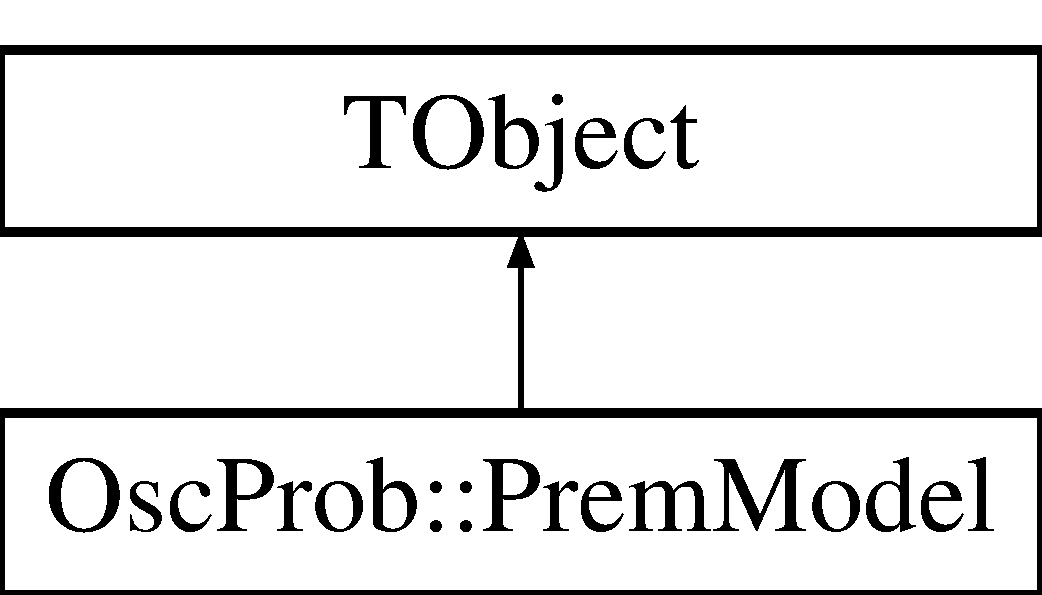
\includegraphics[height=2.000000cm]{classOscProb_1_1PremModel}
\end{center}
\end{figure}
\subsection*{Public Member Functions}
\begin{DoxyCompactItemize}
\item 
\hyperlink{classOscProb_1_1PremModel_a959f8da5c78881b950bd647b67c1ef9b}{Prem\+Model} (std\+::string filename=\char`\"{}\char`\"{})
\begin{DoxyCompactList}\small\item\em Constructor. \end{DoxyCompactList}\item 
virtual \hyperlink{classOscProb_1_1PremModel_aac484ca4e607f2b0fc6f599358cb95fb}{$\sim$\+Prem\+Model} ()
\begin{DoxyCompactList}\small\item\em Destructor. \end{DoxyCompactList}\item 
virtual int \hyperlink{classOscProb_1_1PremModel_ac69162cc5e3c8b7c1b8a85571ff2063b}{Fill\+Path} (double cosT)
\begin{DoxyCompactList}\small\item\em Fill the path sequence in a vector. \end{DoxyCompactList}\item 
virtual std\+::vector$<$ \hyperlink{structOscProb_1_1NuPath}{Osc\+Prob\+::\+Nu\+Path} $>$ \hyperlink{classOscProb_1_1PremModel_adbe7a5df260cba3923f5cbcb8ab2f03f}{Get\+Nu\+Path} ()
\begin{DoxyCompactList}\small\item\em Get the current neutrino path sequence. \end{DoxyCompactList}\item 
virtual std\+::vector$<$ \hyperlink{structOscProb_1_1NuPath}{Osc\+Prob\+::\+Nu\+Path} $>$ \hyperlink{classOscProb_1_1PremModel_a5b6f83f2e9b7087e8faad1f19f00ebd5}{Get\+Merged\+Paths} (double prec=0.\+25)
\begin{DoxyCompactList}\small\item\em Get merged path sequence in a vector. \end{DoxyCompactList}\item 
virtual double \hyperlink{classOscProb_1_1PremModel_ae258b41cca80631e3041f0421b25afeb}{Get\+TotalL} (double cosT)
\begin{DoxyCompactList}\small\item\em Get the total baseline for a given cos\+Theta. \end{DoxyCompactList}\item 
virtual double \hyperlink{classOscProb_1_1PremModel_a5328474bdbb703eb4c9d4df49999cda6}{Get\+CosT} (double L)
\begin{DoxyCompactList}\small\item\em Get the cos\+Theta for a given total baseline. \end{DoxyCompactList}\item 
virtual void \hyperlink{classOscProb_1_1PremModel_ac9887d1af4b3c02925fe3228349f593d}{Set\+Layer\+ZoA} (int layer, double zoa)
\begin{DoxyCompactList}\small\item\em Set Z/A of all layers of a given type. \end{DoxyCompactList}\item 
virtual double \hyperlink{classOscProb_1_1PremModel_af1b8392d1b00560c6322bf8707c304f6}{Get\+Layer\+ZoA} (int layer)
\begin{DoxyCompactList}\small\item\em Get Z/A of all layers of a given type. \end{DoxyCompactList}\item 
virtual void \hyperlink{classOscProb_1_1PremModel_a095bd601f6cd91926de9928e96ea7751}{Set\+Top\+Layer\+Size} (double thick)
\begin{DoxyCompactList}\small\item\em Set the outermost layer thickness in km. \end{DoxyCompactList}\item 
virtual void \hyperlink{classOscProb_1_1PremModel_a6363a5e711dd8b0d2e684677e585b293}{Load\+Model} (std\+::string filename)
\begin{DoxyCompactList}\small\item\em Load an earth model from a file. \end{DoxyCompactList}\item 
virtual void \hyperlink{classOscProb_1_1PremModel_a55b314e97ed9b92931e08ada0c0947eb}{Set\+Det\+Pos} (double pos)
\begin{DoxyCompactList}\small\item\em Set the detector position in km. \end{DoxyCompactList}\item 
virtual std\+::vector$<$ \hyperlink{structOscProb_1_1PremLayer}{Osc\+Prob\+::\+Prem\+Layer} $>$ \hyperlink{classOscProb_1_1PremModel_ae4feeccc7027253f5c2e2493098145ca}{Get\+Prem\+Layers} ()
\begin{DoxyCompactList}\small\item\em Get the set of earth layers. \end{DoxyCompactList}\item 
virtual void \hyperlink{classOscProb_1_1PremModel_ac5496d6d5bafcf7740c60838d3eee7b3}{Set\+Remove\+Small\+Paths} (bool rp=true)
\begin{DoxyCompactList}\small\item\em Set tag to remove small paths. \end{DoxyCompactList}\end{DoxyCompactItemize}
\subsection*{Protected Member Functions}
\begin{DoxyCompactItemize}
\item 
virtual void \hyperlink{classOscProb_1_1PremModel_aaead53a9385bda9b0219fd051d0cdd11}{Clear\+Model} ()
\begin{DoxyCompactList}\small\item\em Clear the earth model information. \end{DoxyCompactList}\item 
virtual void \hyperlink{classOscProb_1_1PremModel_a08c337b84138adc46ee4dd002e9262d2}{Add\+Layer} (double radius, double density, double zoa, double layer)
\begin{DoxyCompactList}\small\item\em Add a layer to the model. \end{DoxyCompactList}\item 
virtual void \hyperlink{classOscProb_1_1PremModel_aca013f7ac5494282834048786a0e07a6}{Add\+Path} (double length, \hyperlink{structOscProb_1_1PremLayer}{Prem\+Layer} pl)
\begin{DoxyCompactList}\small\item\em Add a path segment to the sequence. \end{DoxyCompactList}\item 
\hyperlink{classOscProb_1_1PremModel_a9a1d78e29217bb0dd00ae3bd96d22b69}{Class\+Def} (\hyperlink{classOscProb_1_1PremModel}{Prem\+Model}, 1)
\end{DoxyCompactItemize}
\subsection*{Protected Attributes}
\begin{DoxyCompactItemize}
\item 
std\+::vector$<$ \hyperlink{structOscProb_1_1PremLayer}{Osc\+Prob\+::\+Prem\+Layer} $>$ \hyperlink{classOscProb_1_1PremModel_a19a9a3b23ec154ad7a29f92b74aa5bc6}{f\+Prem\+Layers}
\begin{DoxyCompactList}\small\item\em The layers in the earth model. \end{DoxyCompactList}\item 
std\+::vector$<$ \hyperlink{structOscProb_1_1NuPath}{Osc\+Prob\+::\+Nu\+Path} $>$ \hyperlink{classOscProb_1_1PremModel_aaf3c77e35798d664853157013c90ad2b}{f\+Nu\+Path}
\begin{DoxyCompactList}\small\item\em The current neutrino path sequence. \end{DoxyCompactList}\item 
int \hyperlink{classOscProb_1_1PremModel_a4fb68506493666349f418b893a996185}{f\+Det\+Layer}
\begin{DoxyCompactList}\small\item\em The layer index of the detector. \end{DoxyCompactList}\item 
double \hyperlink{classOscProb_1_1PremModel_ab12ea0343cd11b9233ffd20ab5e620c7}{f\+Det\+Pos}
\begin{DoxyCompactList}\small\item\em The radius where the detector lives. \end{DoxyCompactList}\item 
bool \hyperlink{classOscProb_1_1PremModel_a3973df6f5f2ff219cd2f865b31aacfd2}{f\+Remove\+Small\+Paths}
\begin{DoxyCompactList}\small\item\em Tag whether to merge small paths. \end{DoxyCompactList}\end{DoxyCompactItemize}
\subsection*{Static Protected Attributes}
\begin{DoxyCompactItemize}
\item 
static const double \hyperlink{classOscProb_1_1PremModel_a8ad1335ebe80ee1cd1cdf59d774ab34b}{D\+E\+T\+\_\+\+T\+OL} = 0.\+2
\begin{DoxyCompactList}\small\item\em The detector position tolerance near boundaries. \end{DoxyCompactList}\end{DoxyCompactItemize}


\subsection{Detailed Description}
This class implements a spherically symmetric model of the earth using \hyperlink{structOscProb_1_1PremLayer}{Prem\+Layer}\textquotesingle{}s to store spherical shells with different properties.

The class is then able to produce path sequences through the different earth layers as a function of the cosine of the zenith angle with respect to the detector.

The detector can be positioned at any radius within the model and the path sequences will take into account the fact that some layers are above the detector.

By default this implements the model stored in Prem\+Tables/prem\+\_\+default.\+txt with the detector at the bottom of the ocean layer (radius = 6368 km).

This class inherits from T\+Object and can be saved in R\+O\+OT files.

\begin{DoxyAuthor}{Author}
coelho@lal.\+in2p3.\+fr 
\end{DoxyAuthor}


Definition at line 37 of file Prem\+Model.\+h.



\subsection{Constructor \& Destructor Documentation}
\mbox{\Hypertarget{classOscProb_1_1PremModel_a959f8da5c78881b950bd647b67c1ef9b}\label{classOscProb_1_1PremModel_a959f8da5c78881b950bd647b67c1ef9b}} 
\index{Osc\+Prob\+::\+Prem\+Model@{Osc\+Prob\+::\+Prem\+Model}!Prem\+Model@{Prem\+Model}}
\index{Prem\+Model@{Prem\+Model}!Osc\+Prob\+::\+Prem\+Model@{Osc\+Prob\+::\+Prem\+Model}}
\subsubsection{\texorpdfstring{Prem\+Model()}{PremModel()}}
{\footnotesize\ttfamily Prem\+Model\+::\+Prem\+Model (\begin{DoxyParamCaption}\item[{std\+::string}]{filename = {\ttfamily \char`\"{}\char`\"{}} }\end{DoxyParamCaption})}

Constructor.

By default this implements the model stored in Prem\+Tables/prem\+\_\+default.\+txt with the detector at the bottom of the ocean layer (radius = 6368 km).


\begin{DoxyParams}{Parameters}
{\em filename} & -\/ The txt file containing a table of earth layers \\
\hline
\end{DoxyParams}


Definition at line 35 of file Prem\+Model.\+cxx.



References Load\+Model(), and Set\+Det\+Pos().


\begin{DoxyCode}
35                                     :
36 \hyperlink{classOscProb_1_1PremModel_a4fb68506493666349f418b893a996185}{fDetLayer}(0), \hyperlink{classOscProb_1_1PremModel_a3973df6f5f2ff219cd2f865b31aacfd2}{fRemoveSmallPaths}(\textcolor{keyword}{false})
37 \{
38 
39   \hyperlink{classOscProb_1_1PremModel_a55b314e97ed9b92931e08ada0c0947eb}{SetDetPos}(6368);
40   \hyperlink{classOscProb_1_1PremModel_a6363a5e711dd8b0d2e684677e585b293}{LoadModel}(filename);
41 
42 \}
\end{DoxyCode}
\mbox{\Hypertarget{classOscProb_1_1PremModel_aac484ca4e607f2b0fc6f599358cb95fb}\label{classOscProb_1_1PremModel_aac484ca4e607f2b0fc6f599358cb95fb}} 
\index{Osc\+Prob\+::\+Prem\+Model@{Osc\+Prob\+::\+Prem\+Model}!````~Prem\+Model@{$\sim$\+Prem\+Model}}
\index{````~Prem\+Model@{$\sim$\+Prem\+Model}!Osc\+Prob\+::\+Prem\+Model@{Osc\+Prob\+::\+Prem\+Model}}
\subsubsection{\texorpdfstring{$\sim$\+Prem\+Model()}{~PremModel()}}
{\footnotesize\ttfamily Prem\+Model\+::$\sim$\+Prem\+Model (\begin{DoxyParamCaption}{ }\end{DoxyParamCaption})\hspace{0.3cm}{\ttfamily [virtual]}}

Nothing to clean. 

Definition at line 48 of file Prem\+Model.\+cxx.


\begin{DoxyCode}
48 \{\}
\end{DoxyCode}


\subsection{Member Function Documentation}
\mbox{\Hypertarget{classOscProb_1_1PremModel_a08c337b84138adc46ee4dd002e9262d2}\label{classOscProb_1_1PremModel_a08c337b84138adc46ee4dd002e9262d2}} 
\index{Osc\+Prob\+::\+Prem\+Model@{Osc\+Prob\+::\+Prem\+Model}!Add\+Layer@{Add\+Layer}}
\index{Add\+Layer@{Add\+Layer}!Osc\+Prob\+::\+Prem\+Model@{Osc\+Prob\+::\+Prem\+Model}}
\subsubsection{\texorpdfstring{Add\+Layer()}{AddLayer()}}
{\footnotesize\ttfamily void Prem\+Model\+::\+Add\+Layer (\begin{DoxyParamCaption}\item[{double}]{radius,  }\item[{double}]{density,  }\item[{double}]{zoa,  }\item[{double}]{layer }\end{DoxyParamCaption})\hspace{0.3cm}{\ttfamily [protected]}, {\ttfamily [virtual]}}

Add a layer to the earth model.


\begin{DoxyParams}{Parameters}
{\em radius} & -\/ The outer radius of the layer in km \\
\hline
{\em density} & -\/ The density of the layer in g/cm$^\wedge$3 \\
\hline
{\em zoa} & -\/ The effective Z/A value of the layer \\
\hline
{\em layer} & -\/ An index to identify the matter type (e.\+g. earth inner core) \\
\hline
\end{DoxyParams}


Definition at line 105 of file Prem\+Model.\+cxx.



References f\+Prem\+Layers.



Referenced by Load\+Model().


\begin{DoxyCode}
107 \{
108 
109   \hyperlink{classOscProb_1_1PremModel_a19a9a3b23ec154ad7a29f92b74aa5bc6}{fPremLayers}.push\_back( \hyperlink{structOscProb_1_1PremLayer}{PremLayer}(radius, density, zoa, layer) );
110 
111 \}
\end{DoxyCode}
\mbox{\Hypertarget{classOscProb_1_1PremModel_aca013f7ac5494282834048786a0e07a6}\label{classOscProb_1_1PremModel_aca013f7ac5494282834048786a0e07a6}} 
\index{Osc\+Prob\+::\+Prem\+Model@{Osc\+Prob\+::\+Prem\+Model}!Add\+Path@{Add\+Path}}
\index{Add\+Path@{Add\+Path}!Osc\+Prob\+::\+Prem\+Model@{Osc\+Prob\+::\+Prem\+Model}}
\subsubsection{\texorpdfstring{Add\+Path()}{AddPath()}}
{\footnotesize\ttfamily void Prem\+Model\+::\+Add\+Path (\begin{DoxyParamCaption}\item[{double}]{length,  }\item[{\hyperlink{structOscProb_1_1PremLayer}{Prem\+Layer}}]{pl }\end{DoxyParamCaption})\hspace{0.3cm}{\ttfamily [protected]}, {\ttfamily [virtual]}}

Add a path segment to the sequence.

For a given \hyperlink{structOscProb_1_1PremLayer}{Prem\+Layer}, adds a path of a given length in that material


\begin{DoxyParams}{Parameters}
{\em length} & -\/ The length of the path segment in km \\
\hline
{\em pl} & -\/ The layer we are crossing \\
\hline
\end{DoxyParams}


Definition at line 336 of file Prem\+Model.\+cxx.



References Osc\+Prob\+::\+Prem\+Layer\+::density, f\+Nu\+Path, Osc\+Prob\+::\+Prem\+Layer\+::layer, and Osc\+Prob\+::\+Prem\+Layer\+::zoa.



Referenced by Fill\+Path().


\begin{DoxyCode}
337 \{
338 
339   \hyperlink{classOscProb_1_1PremModel_aaf3c77e35798d664853157013c90ad2b}{fNuPath}.push\_back( \hyperlink{structOscProb_1_1NuPath}{NuPath}(length, pl.\hyperlink{structOscProb_1_1PremLayer_aba2536cbdab87d0db33df47f95c4f2c3}{density}, pl.\hyperlink{structOscProb_1_1PremLayer_a8687a8169d786fca79908292d11077f5}{zoa}, pl.
      \hyperlink{structOscProb_1_1PremLayer_aca8d7df68e6f982155b68b7e6a7ef389}{layer}) );
340 
341 \}
\end{DoxyCode}
\mbox{\Hypertarget{classOscProb_1_1PremModel_a9a1d78e29217bb0dd00ae3bd96d22b69}\label{classOscProb_1_1PremModel_a9a1d78e29217bb0dd00ae3bd96d22b69}} 
\index{Osc\+Prob\+::\+Prem\+Model@{Osc\+Prob\+::\+Prem\+Model}!Class\+Def@{Class\+Def}}
\index{Class\+Def@{Class\+Def}!Osc\+Prob\+::\+Prem\+Model@{Osc\+Prob\+::\+Prem\+Model}}
\subsubsection{\texorpdfstring{Class\+Def()}{ClassDef()}}
{\footnotesize\ttfamily Osc\+Prob\+::\+Prem\+Model\+::\+Class\+Def (\begin{DoxyParamCaption}\item[{\hyperlink{classOscProb_1_1PremModel}{Prem\+Model}}]{,  }\item[{1}]{ }\end{DoxyParamCaption})\hspace{0.3cm}{\ttfamily [protected]}}

\mbox{\Hypertarget{classOscProb_1_1PremModel_aaead53a9385bda9b0219fd051d0cdd11}\label{classOscProb_1_1PremModel_aaead53a9385bda9b0219fd051d0cdd11}} 
\index{Osc\+Prob\+::\+Prem\+Model@{Osc\+Prob\+::\+Prem\+Model}!Clear\+Model@{Clear\+Model}}
\index{Clear\+Model@{Clear\+Model}!Osc\+Prob\+::\+Prem\+Model@{Osc\+Prob\+::\+Prem\+Model}}
\subsubsection{\texorpdfstring{Clear\+Model()}{ClearModel()}}
{\footnotesize\ttfamily void Prem\+Model\+::\+Clear\+Model (\begin{DoxyParamCaption}{ }\end{DoxyParamCaption})\hspace{0.3cm}{\ttfamily [protected]}, {\ttfamily [virtual]}}

Clear the earth model information. 

Definition at line 88 of file Prem\+Model.\+cxx.



References f\+Det\+Layer, and f\+Prem\+Layers.



Referenced by Load\+Model().


\begin{DoxyCode}
89 \{
90 
91   \hyperlink{classOscProb_1_1PremModel_a4fb68506493666349f418b893a996185}{fDetLayer} = 0;
92   \hyperlink{classOscProb_1_1PremModel_a19a9a3b23ec154ad7a29f92b74aa5bc6}{fPremLayers}.clear();
93 
94 \}
\end{DoxyCode}
\mbox{\Hypertarget{classOscProb_1_1PremModel_ac69162cc5e3c8b7c1b8a85571ff2063b}\label{classOscProb_1_1PremModel_ac69162cc5e3c8b7c1b8a85571ff2063b}} 
\index{Osc\+Prob\+::\+Prem\+Model@{Osc\+Prob\+::\+Prem\+Model}!Fill\+Path@{Fill\+Path}}
\index{Fill\+Path@{Fill\+Path}!Osc\+Prob\+::\+Prem\+Model@{Osc\+Prob\+::\+Prem\+Model}}
\subsubsection{\texorpdfstring{Fill\+Path()}{FillPath()}}
{\footnotesize\ttfamily int Prem\+Model\+::\+Fill\+Path (\begin{DoxyParamCaption}\item[{double}]{cosT }\end{DoxyParamCaption})\hspace{0.3cm}{\ttfamily [virtual]}}

Fill the path sequence in a vector.

This will start at the upper-\/most layer and find straight paths to the boundary of the next layer down. When reaching the inner-\/most layer in the given direction, the paths move back to outer layers until hitting the detector.

The path sequence is stored as an attribute and can be retrieved with the function Get\+Nu\+Path.


\begin{DoxyParams}{Parameters}
{\em cosT} & -\/ The cosine of the neutrino direction \\
\hline
\end{DoxyParams}
\begin{DoxyReturn}{Returns}
The number of path segments in the sequence 
\end{DoxyReturn}


Definition at line 358 of file Prem\+Model.\+cxx.



References Add\+Path(), f\+Det\+Layer, f\+Nu\+Path, and f\+Prem\+Layers.


\begin{DoxyCode}
359 \{
360 
361   \textcolor{comment}{// Clear current path sequence}
362   \hyperlink{classOscProb_1_1PremModel_aaf3c77e35798d664853157013c90ad2b}{fNuPath}.clear();
363 
364   \textcolor{comment}{// Do nothing if cosine is unphysical}
365   \textcolor{keywordflow}{if}(fabs(cosT) > 1) \textcolor{keywordflow}{return} 0;
366 
367   \textcolor{comment}{// Define the minimum path radius}
368   \textcolor{keywordtype}{double} minR = \hyperlink{classOscProb_1_1PremModel_a19a9a3b23ec154ad7a29f92b74aa5bc6}{fPremLayers}[\hyperlink{classOscProb_1_1PremModel_a4fb68506493666349f418b893a996185}{fDetLayer}].radius * sqrt(1 - cosT*cosT);
369 
370   \textcolor{comment}{// Set the top layer index}
371   \textcolor{keywordtype}{int} toplayer = \hyperlink{classOscProb_1_1PremModel_a19a9a3b23ec154ad7a29f92b74aa5bc6}{fPremLayers}.size() - 1;
372 
373   \textcolor{comment}{// Find the inner-most crossed layer}
374   \textcolor{keywordtype}{int} minlayer = 0;
375   \textcolor{keywordflow}{while}(\hyperlink{classOscProb_1_1PremModel_a19a9a3b23ec154ad7a29f92b74aa5bc6}{fPremLayers}[minlayer].radius < minR) minlayer++;
376 
377   \textcolor{comment}{// Compute the number of path segments needed}
378   \textcolor{keywordtype}{int} nsteps = toplayer - \hyperlink{classOscProb_1_1PremModel_a4fb68506493666349f418b893a996185}{fDetLayer};
379   \textcolor{keywordflow}{if}(cosT < 0) nsteps += 2*(fDetLayer - minlayer) + 1;
380 
381   \textcolor{comment}{// Start at the top layer and go down}
382   \textcolor{keywordtype}{int} layer = toplayer;
383   \textcolor{keywordtype}{int} dl = -1;
384 
385   \textcolor{comment}{// Loop over all path segments}
386   \textcolor{keywordflow}{for}(\textcolor{keywordtype}{int} i=0; i<nsteps; i++)\{
387 
388     \textcolor{comment}{// Get square of the path length between this layer's}
389     \textcolor{comment}{// outer radius and  inner-most radius}
390     \textcolor{keywordtype}{double} L1 = pow(\hyperlink{classOscProb_1_1PremModel_a19a9a3b23ec154ad7a29f92b74aa5bc6}{fPremLayers}[layer].radius,2) - minR*minR;
391 
392     \textcolor{comment}{// If L1 is negative, outer radius is not crossed.}
393     \textcolor{comment}{// This only happens if detector is at the top layer and the}
394     \textcolor{comment}{// neutrino is coming from above.}
395     \textcolor{keywordflow}{if}(L1 < 0) \textcolor{keywordflow}{return} \textcolor{keyword}{true};
396 
397     \textcolor{comment}{// Get square of the path length between this layer's}
398     \textcolor{comment}{// inner radius and  inner-most radius}
399     \textcolor{keywordtype}{double} L2 = -minR*minR;
400     \textcolor{keywordflow}{if}(layer>0) L2 += pow(\hyperlink{classOscProb_1_1PremModel_a19a9a3b23ec154ad7a29f92b74aa5bc6}{fPremLayers}[layer-1].radius,2);
401 
402     \textcolor{comment}{// If L2 is negative, inner radius is not crossed,}
403     \textcolor{comment}{// so set this as the minimum layer.}
404     \textcolor{keywordtype}{bool} ismin = (L2<=0 && cosT < 0);
405 
406     \textcolor{comment}{// Store the path segment length}
407     \textcolor{keywordtype}{double} dL;
408 
409     \textcolor{comment}{// If it's the minimum layer, connect two outer radius}
410     \textcolor{comment}{// crossing points. If not, compute difference between}
411     \textcolor{comment}{// inner and outer radius crossings.}
412     \textcolor{keywordflow}{if}(ismin)      dL = 2 * sqrt(L1);
413     \textcolor{keywordflow}{else} \textcolor{keywordflow}{if}(L2>=0) dL = sqrt(L1) - sqrt(L2);
414     \textcolor{keywordflow}{else}           dL = sqrt(L1); \textcolor{comment}{// This should never actually happen,}
415                                   \textcolor{comment}{// but protect in case L2 is slightly}
416                                   \textcolor{comment}{// negative when it should be zero.}
417                                   \textcolor{comment}{// e.g. arriving at the detector from above.}
418 
419     \textcolor{comment}{// Add this path segment to the sequence}
420     \hyperlink{classOscProb_1_1PremModel_aca013f7ac5494282834048786a0e07a6}{AddPath}(dL, \hyperlink{classOscProb_1_1PremModel_a19a9a3b23ec154ad7a29f92b74aa5bc6}{fPremLayers}[layer]);
421 
422     \textcolor{comment}{// If we reached the inner-most layer,}
423     \textcolor{comment}{// start moving up again.}
424     \textcolor{keywordflow}{if}(ismin) dl = 1;
425 
426     \textcolor{comment}{// Move to next layer}
427     layer += dl;
428 
429   \}
430 
431   \textcolor{comment}{// Return the number of path segments}
432   \textcolor{keywordflow}{return} \hyperlink{classOscProb_1_1PremModel_aaf3c77e35798d664853157013c90ad2b}{fNuPath}.size();
433 
434 \}
\end{DoxyCode}
\mbox{\Hypertarget{classOscProb_1_1PremModel_a5328474bdbb703eb4c9d4df49999cda6}\label{classOscProb_1_1PremModel_a5328474bdbb703eb4c9d4df49999cda6}} 
\index{Osc\+Prob\+::\+Prem\+Model@{Osc\+Prob\+::\+Prem\+Model}!Get\+CosT@{Get\+CosT}}
\index{Get\+CosT@{Get\+CosT}!Osc\+Prob\+::\+Prem\+Model@{Osc\+Prob\+::\+Prem\+Model}}
\subsubsection{\texorpdfstring{Get\+Cos\+T()}{GetCosT()}}
{\footnotesize\ttfamily double Prem\+Model\+::\+Get\+CosT (\begin{DoxyParamCaption}\item[{double}]{L }\end{DoxyParamCaption})\hspace{0.3cm}{\ttfamily [virtual]}}

Get the cos\+Theta for a given total baseline.

Given a baseline, find the direction of the neutrino. This could be useful for experiments with fixed baselines for example.

The baseline must be within the range of possible values in this earth model. Will return vertical neutrinos otherwise.


\begin{DoxyParams}{Parameters}
{\em L} & -\/ The total baseline of the neutrino \\
\hline
\end{DoxyParams}


Definition at line 314 of file Prem\+Model.\+cxx.



References f\+Det\+Layer, and f\+Prem\+Layers.


\begin{DoxyCode}
315 \{
316 
317   \textcolor{keywordtype}{double} rAbove = \hyperlink{classOscProb_1_1PremModel_a19a9a3b23ec154ad7a29f92b74aa5bc6}{fPremLayers}.back().radius;     \textcolor{comment}{// Radius above detector}
318   \textcolor{keywordtype}{double} rBelow = \hyperlink{classOscProb_1_1PremModel_a19a9a3b23ec154ad7a29f92b74aa5bc6}{fPremLayers}[\hyperlink{classOscProb_1_1PremModel_a4fb68506493666349f418b893a996185}{fDetLayer}].radius; \textcolor{comment}{// Radius below detector}
319 
320   \textcolor{keywordflow}{if}(L < rAbove - rBelow) \textcolor{keywordflow}{return}  1;
321   \textcolor{keywordflow}{if}(L > rAbove + rBelow) \textcolor{keywordflow}{return} -1;
322 
323   \textcolor{keywordflow}{return} (rAbove*rAbove - rBelow*rBelow - L*L) / (2*rBelow*L);
324 
325 \}
\end{DoxyCode}
\mbox{\Hypertarget{classOscProb_1_1PremModel_af1b8392d1b00560c6322bf8707c304f6}\label{classOscProb_1_1PremModel_af1b8392d1b00560c6322bf8707c304f6}} 
\index{Osc\+Prob\+::\+Prem\+Model@{Osc\+Prob\+::\+Prem\+Model}!Get\+Layer\+ZoA@{Get\+Layer\+ZoA}}
\index{Get\+Layer\+ZoA@{Get\+Layer\+ZoA}!Osc\+Prob\+::\+Prem\+Model@{Osc\+Prob\+::\+Prem\+Model}}
\subsubsection{\texorpdfstring{Get\+Layer\+Zo\+A()}{GetLayerZoA()}}
{\footnotesize\ttfamily double Prem\+Model\+::\+Get\+Layer\+ZoA (\begin{DoxyParamCaption}\item[{int}]{layer }\end{DoxyParamCaption})\hspace{0.3cm}{\ttfamily [virtual]}}

Get the effective Z/A value for all layers of a given type, e.\+g. all outer-\/core layers.


\begin{DoxyParams}{Parameters}
{\em layer} & -\/ The index of the layer type \\
\hline
\end{DoxyParams}


Definition at line 220 of file Prem\+Model.\+cxx.



References f\+Prem\+Layers.


\begin{DoxyCode}
221 \{
222 
223   \textcolor{keywordtype}{int} nlayers = \hyperlink{classOscProb_1_1PremModel_a19a9a3b23ec154ad7a29f92b74aa5bc6}{fPremLayers}.size();
224 
225   \textcolor{comment}{// This check assumes the layer types are in increasing order}
226   \textcolor{keywordflow}{if}(layer > \hyperlink{classOscProb_1_1PremModel_a19a9a3b23ec154ad7a29f92b74aa5bc6}{fPremLayers}.back().layer)\{
227     cout << \textcolor{stringliteral}{"ERROR: Not that many layer types"} << endl;
228     cout << \textcolor{stringliteral}{"Returning 0"} << endl;
229     \textcolor{keywordflow}{return} 0;
230   \}
231 
232   \textcolor{keywordflow}{for}(\textcolor{keywordtype}{int} i=0; i<nlayers; i++)\{
233 
234     \textcolor{keywordflow}{if}(\hyperlink{classOscProb_1_1PremModel_a19a9a3b23ec154ad7a29f92b74aa5bc6}{fPremLayers}[i].layer != layer) \textcolor{keywordflow}{continue};
235 
236     \textcolor{keywordflow}{else} \textcolor{keywordflow}{return} \hyperlink{classOscProb_1_1PremModel_a19a9a3b23ec154ad7a29f92b74aa5bc6}{fPremLayers}[i].zoa;
237 
238   \}
239 
240   \textcolor{comment}{// End of vector reached without finding input type}
241   cout << \textcolor{stringliteral}{"ERROR: layer type not found"} << endl;
242   cout << \textcolor{stringliteral}{"Returning 0"} << endl;
243   \textcolor{keywordflow}{return} 0;
244 \}
\end{DoxyCode}
\mbox{\Hypertarget{classOscProb_1_1PremModel_a5b6f83f2e9b7087e8faad1f19f00ebd5}\label{classOscProb_1_1PremModel_a5b6f83f2e9b7087e8faad1f19f00ebd5}} 
\index{Osc\+Prob\+::\+Prem\+Model@{Osc\+Prob\+::\+Prem\+Model}!Get\+Merged\+Paths@{Get\+Merged\+Paths}}
\index{Get\+Merged\+Paths@{Get\+Merged\+Paths}!Osc\+Prob\+::\+Prem\+Model@{Osc\+Prob\+::\+Prem\+Model}}
\subsubsection{\texorpdfstring{Get\+Merged\+Paths()}{GetMergedPaths()}}
{\footnotesize\ttfamily vector$<$ \hyperlink{structOscProb_1_1NuPath}{Nu\+Path} $>$ Prem\+Model\+::\+Get\+Merged\+Paths (\begin{DoxyParamCaption}\item[{double}]{prec = {\ttfamily 0.25} }\end{DoxyParamCaption})\hspace{0.3cm}{\ttfamily [virtual]}}

Merge similar paths to reduce number of steps

This method will merge consecutive paths and take their averages until it finds a large enough gap to start a new merged path.

The merged paths will be returned, and the original detailed path will not be changed and will stay stored as an attribute.


\begin{DoxyParams}{Parameters}
{\em prec} & -\/ The precision to merge paths in g/cm$^\wedge$3 \\
\hline
\end{DoxyParams}
\begin{DoxyReturn}{Returns}
The vector of merged path segments 
\end{DoxyReturn}


Definition at line 449 of file Prem\+Model.\+cxx.



References Osc\+Prob\+::\+Avg\+Path(), Osc\+Prob\+::\+Nu\+Path\+::density, f\+Nu\+Path, f\+Remove\+Small\+Paths, Osc\+Prob\+::\+Merge\+Paths(), and Osc\+Prob\+::\+Nu\+Path\+::zoa.


\begin{DoxyCode}
449                                                    \{
450 
451   \textcolor{comment}{// The output vector}
452   vector<NuPath> mergedPath;
453 
454   \textcolor{comment}{// Start with the first path}
455   \hyperlink{structOscProb_1_1NuPath}{OscProb::NuPath} path = \hyperlink{classOscProb_1_1PremModel_aaf3c77e35798d664853157013c90ad2b}{fNuPath}[0];
456 
457   \textcolor{comment}{// Track the total length}
458   \textcolor{keywordtype}{double} totL = 0;
459 
460   \textcolor{comment}{// Loop over all paths starting from second}
461   \textcolor{keywordflow}{for}(\textcolor{keywordtype}{int} i=1; i<\hyperlink{classOscProb_1_1PremModel_aaf3c77e35798d664853157013c90ad2b}{fNuPath}.size(); i++)\{
462 
463     \textcolor{comment}{// If this path electron density is beyond the tolerance}
464     \textcolor{keywordflow}{if}( fabs(path.\hyperlink{structOscProb_1_1NuPath_a54ddd451db69bc54434de3cf18a117ca}{density}*path.\hyperlink{structOscProb_1_1NuPath_af3213f3691ba83c6bc05f4a3490f6b31}{zoa} - \hyperlink{classOscProb_1_1PremModel_aaf3c77e35798d664853157013c90ad2b}{fNuPath}[i].density*\hyperlink{classOscProb_1_1PremModel_aaf3c77e35798d664853157013c90ad2b}{fNuPath}[i].zoa) > prec*path
      .\hyperlink{structOscProb_1_1NuPath_af3213f3691ba83c6bc05f4a3490f6b31}{zoa} )\{
465 
466       \textcolor{comment}{// Add merged path to vector}
467       mergedPath.push\_back(path);
468 
469       \textcolor{comment}{// Set this path as new merged path}
470       path = \hyperlink{classOscProb_1_1PremModel_aaf3c77e35798d664853157013c90ad2b}{fNuPath}[i];
471 
472     \}
473     \textcolor{comment}{// If path is within tolerance}
474     \textcolor{keywordflow}{else}\{
475 
476       \textcolor{comment}{// Merge the path with current merged path}
477       path = \hyperlink{namespaceOscProb_a999a7944bad8bc72d7ee9f56f81a210e}{OscProb::AvgPath}(path, \hyperlink{classOscProb_1_1PremModel_aaf3c77e35798d664853157013c90ad2b}{fNuPath}[i]);
478 
479     \}
480 
481     \textcolor{comment}{// Increment total length}
482     totL += \hyperlink{classOscProb_1_1PremModel_aaf3c77e35798d664853157013c90ad2b}{fNuPath}[i].length;
483 
484   \}\textcolor{comment}{// End of loop over paths}
485 
486   \textcolor{comment}{// Add the final merged path to vector}
487   mergedPath.push\_back(path);
488 
489   \textcolor{comment}{// If tag is true, remove small paths}
490   \textcolor{keywordflow}{if}(\hyperlink{classOscProb_1_1PremModel_a3973df6f5f2ff219cd2f865b31aacfd2}{fRemoveSmallPaths})\{
491 
492     \textcolor{comment}{// Start at first path}
493     \textcolor{keywordtype}{int} k = 0;
494 
495     \textcolor{comment}{// While not at the end of vector}
496     \textcolor{keywordflow}{while}(k + 1 < mergedPath.size())\{
497 
498       \textcolor{comment}{// If length is less than 1% of total}
499       \textcolor{keywordflow}{if}(mergedPath[k].length < 0.01*totL)\{
500 
501         \textcolor{comment}{// Merge path with following path}
502         mergedPath = \hyperlink{namespaceOscProb_a7c203d8583a34acf2ae90185ba45f866}{MergePaths}(mergedPath, k, k+1);
503 
504       \}
505       \textcolor{comment}{// If path is long enough skip it}
506       \textcolor{keywordflow}{else} k++;
507 
508     \}\textcolor{comment}{// End of while loop}
509 
510   \}\textcolor{comment}{// End of if statement}
511 
512   \textcolor{comment}{// return the merged vector}
513   \textcolor{keywordflow}{return} mergedPath;
514 
515 \}
\end{DoxyCode}
\mbox{\Hypertarget{classOscProb_1_1PremModel_adbe7a5df260cba3923f5cbcb8ab2f03f}\label{classOscProb_1_1PremModel_adbe7a5df260cba3923f5cbcb8ab2f03f}} 
\index{Osc\+Prob\+::\+Prem\+Model@{Osc\+Prob\+::\+Prem\+Model}!Get\+Nu\+Path@{Get\+Nu\+Path}}
\index{Get\+Nu\+Path@{Get\+Nu\+Path}!Osc\+Prob\+::\+Prem\+Model@{Osc\+Prob\+::\+Prem\+Model}}
\subsubsection{\texorpdfstring{Get\+Nu\+Path()}{GetNuPath()}}
{\footnotesize\ttfamily vector$<$ \hyperlink{structOscProb_1_1NuPath}{Nu\+Path} $>$ Prem\+Model\+::\+Get\+Nu\+Path (\begin{DoxyParamCaption}{ }\end{DoxyParamCaption})\hspace{0.3cm}{\ttfamily [virtual]}}

Get the current neutrino path sequence

The path needs to be filled for a given cos\+Theta before calling this function. 

Definition at line 73 of file Prem\+Model.\+cxx.



References f\+Nu\+Path.


\begin{DoxyCode}
73 \{ \textcolor{keywordflow}{return} \hyperlink{classOscProb_1_1PremModel_aaf3c77e35798d664853157013c90ad2b}{fNuPath}; \}
\end{DoxyCode}
\mbox{\Hypertarget{classOscProb_1_1PremModel_ae4feeccc7027253f5c2e2493098145ca}\label{classOscProb_1_1PremModel_ae4feeccc7027253f5c2e2493098145ca}} 
\index{Osc\+Prob\+::\+Prem\+Model@{Osc\+Prob\+::\+Prem\+Model}!Get\+Prem\+Layers@{Get\+Prem\+Layers}}
\index{Get\+Prem\+Layers@{Get\+Prem\+Layers}!Osc\+Prob\+::\+Prem\+Model@{Osc\+Prob\+::\+Prem\+Model}}
\subsubsection{\texorpdfstring{Get\+Prem\+Layers()}{GetPremLayers()}}
{\footnotesize\ttfamily vector$<$ \hyperlink{structOscProb_1_1PremLayer}{Prem\+Layer} $>$ Prem\+Model\+::\+Get\+Prem\+Layers (\begin{DoxyParamCaption}{ }\end{DoxyParamCaption})\hspace{0.3cm}{\ttfamily [virtual]}}

Get the set of earth layers

This returns the set of \hyperlink{structOscProb_1_1PremLayer}{Prem\+Layer}\textquotesingle{}s for this earth model and detector position. 

Definition at line 82 of file Prem\+Model.\+cxx.



References f\+Prem\+Layers.


\begin{DoxyCode}
82 \{ \textcolor{keywordflow}{return} \hyperlink{classOscProb_1_1PremModel_a19a9a3b23ec154ad7a29f92b74aa5bc6}{fPremLayers}; \}
\end{DoxyCode}
\mbox{\Hypertarget{classOscProb_1_1PremModel_ae258b41cca80631e3041f0421b25afeb}\label{classOscProb_1_1PremModel_ae258b41cca80631e3041f0421b25afeb}} 
\index{Osc\+Prob\+::\+Prem\+Model@{Osc\+Prob\+::\+Prem\+Model}!Get\+TotalL@{Get\+TotalL}}
\index{Get\+TotalL@{Get\+TotalL}!Osc\+Prob\+::\+Prem\+Model@{Osc\+Prob\+::\+Prem\+Model}}
\subsubsection{\texorpdfstring{Get\+Total\+L()}{GetTotalL()}}
{\footnotesize\ttfamily double Prem\+Model\+::\+Get\+TotalL (\begin{DoxyParamCaption}\item[{double}]{cosT }\end{DoxyParamCaption})\hspace{0.3cm}{\ttfamily [virtual]}}

Get the total baseline for a given cos\+Theta.

The total baseline contains both from above and below the detector.


\begin{DoxyParams}{Parameters}
{\em cosT} & -\/ The cosine of the neutrino direction \\
\hline
\end{DoxyParams}


Definition at line 288 of file Prem\+Model.\+cxx.



References f\+Det\+Layer, and f\+Prem\+Layers.


\begin{DoxyCode}
289 \{
290 
291   \textcolor{keywordflow}{if}(fabs(cosT) > 1) \textcolor{keywordflow}{return} 0;
292 
293   \textcolor{keywordtype}{double} rAbove = \hyperlink{classOscProb_1_1PremModel_a19a9a3b23ec154ad7a29f92b74aa5bc6}{fPremLayers}.back().radius;     \textcolor{comment}{// Radius above detector}
294   \textcolor{keywordtype}{double} rBelow = \hyperlink{classOscProb_1_1PremModel_a19a9a3b23ec154ad7a29f92b74aa5bc6}{fPremLayers}[\hyperlink{classOscProb_1_1PremModel_a4fb68506493666349f418b893a996185}{fDetLayer}].radius; \textcolor{comment}{// Radius below detector}
295 
296   \textcolor{keywordtype}{double} sinsqrT = 1 - cosT*cosT;
297 
298   \textcolor{keywordflow}{return} -rBelow*cosT + sqrt(rAbove*rAbove - rBelow*rBelow*sinsqrT);
299 
300 \}
\end{DoxyCode}
\mbox{\Hypertarget{classOscProb_1_1PremModel_a6363a5e711dd8b0d2e684677e585b293}\label{classOscProb_1_1PremModel_a6363a5e711dd8b0d2e684677e585b293}} 
\index{Osc\+Prob\+::\+Prem\+Model@{Osc\+Prob\+::\+Prem\+Model}!Load\+Model@{Load\+Model}}
\index{Load\+Model@{Load\+Model}!Osc\+Prob\+::\+Prem\+Model@{Osc\+Prob\+::\+Prem\+Model}}
\subsubsection{\texorpdfstring{Load\+Model()}{LoadModel()}}
{\footnotesize\ttfamily void Prem\+Model\+::\+Load\+Model (\begin{DoxyParamCaption}\item[{std\+::string}]{filename }\end{DoxyParamCaption})\hspace{0.3cm}{\ttfamily [virtual]}}

Load an earth model from a file.

By default it loads the model stored in Prem\+Tables/prem\+\_\+default.\+txt

The decision of whether to create a layer for the detector position is made in this function, so the detector position must be set before calling this function.


\begin{DoxyParams}{Parameters}
{\em filename} & -\/ The txt file containing a table of earth layers \\
\hline
\end{DoxyParams}


Definition at line 125 of file Prem\+Model.\+cxx.



References Add\+Layer(), Clear\+Model(), D\+E\+T\+\_\+\+T\+OL, f\+Det\+Layer, f\+Det\+Pos, and f\+Prem\+Layers.



Referenced by Prem\+Model().


\begin{DoxyCode}
126 \{
127 
128   \textcolor{comment}{// Clear the current model}
129   \hyperlink{classOscProb_1_1PremModel_aaead53a9385bda9b0219fd051d0cdd11}{ClearModel}();
130 
131   \textcolor{comment}{// Use default if no file provided}
132   \textcolor{keywordflow}{if}(filename == \textcolor{stringliteral}{""})\{
133     filename = PREM\_DEFAULT;
134   \}
135 
136   \textcolor{comment}{// Open the file}
137   ifstream fin;
138   fin.open(filename.c\_str());
139 
140   \textcolor{keywordflow}{if}(!fin)\{
141     cout << \textcolor{stringliteral}{"ERROR: File "} << filename << \textcolor{stringliteral}{" not found!"} << endl;
142     \textcolor{keywordflow}{return};
143   \}
144 
145   \textcolor{comment}{// Variables for storing table rows}
146   \textcolor{keywordtype}{float} radius, density, zoa, layer;
147 
148   \textcolor{comment}{// Flag to mark we've passed the detector}
149   \textcolor{keywordtype}{bool} crossed\_det = \textcolor{keyword}{false};
150 
151   \textcolor{comment}{// Keep track of previous radius}
152   \textcolor{keywordtype}{double} rprev = 0;
153 
154   \textcolor{comment}{// Loop over table rows}
155   \textcolor{keywordflow}{while}(fin >> radius >> density >> zoa >> layer)\{
156 
157     \textcolor{comment}{// Radii must be ordered in model file}
158     \textcolor{keywordflow}{if}(radius <= rprev)\{
159       cout << \textcolor{stringliteral}{"ERROR: Radii are not sorted in increasing order in the model file"} << endl;
160       \hyperlink{classOscProb_1_1PremModel_aaead53a9385bda9b0219fd051d0cdd11}{ClearModel}();
161       \textcolor{keywordflow}{return};
162     \}
163 
164     \textcolor{comment}{// See if we passed the detector and decide whether}
165     \textcolor{comment}{// to create a special layer for it}
166     \textcolor{keywordflow}{if}(radius > \hyperlink{classOscProb_1_1PremModel_ab12ea0343cd11b9233ffd20ab5e620c7}{fDetPos} - \hyperlink{classOscProb_1_1PremModel_a8ad1335ebe80ee1cd1cdf59d774ab34b}{DET\_TOL} && !crossed\_det)\{
167 
168       crossed\_det = \textcolor{keyword}{true};
169 
170       \hyperlink{classOscProb_1_1PremModel_a4fb68506493666349f418b893a996185}{fDetLayer} = \hyperlink{classOscProb_1_1PremModel_a19a9a3b23ec154ad7a29f92b74aa5bc6}{fPremLayers}.size();
171 
172       \textcolor{comment}{// If detector is not near boundary, add a special layer}
173       \textcolor{keywordflow}{if}(radius > \hyperlink{classOscProb_1_1PremModel_ab12ea0343cd11b9233ffd20ab5e620c7}{fDetPos} + \hyperlink{classOscProb_1_1PremModel_a8ad1335ebe80ee1cd1cdf59d774ab34b}{DET\_TOL})\{
174         \hyperlink{classOscProb_1_1PremModel_a08c337b84138adc46ee4dd002e9262d2}{AddLayer}(\hyperlink{classOscProb_1_1PremModel_ab12ea0343cd11b9233ffd20ab5e620c7}{fDetPos}, density, zoa, layer);
175       \}
176 
177     \}
178 
179     \textcolor{comment}{// Add this layer to the model}
180     \hyperlink{classOscProb_1_1PremModel_a08c337b84138adc46ee4dd002e9262d2}{AddLayer}(radius, density, zoa, layer);
181 
182   \}
183 
184 \}
\end{DoxyCode}
\mbox{\Hypertarget{classOscProb_1_1PremModel_a55b314e97ed9b92931e08ada0c0947eb}\label{classOscProb_1_1PremModel_a55b314e97ed9b92931e08ada0c0947eb}} 
\index{Osc\+Prob\+::\+Prem\+Model@{Osc\+Prob\+::\+Prem\+Model}!Set\+Det\+Pos@{Set\+Det\+Pos}}
\index{Set\+Det\+Pos@{Set\+Det\+Pos}!Osc\+Prob\+::\+Prem\+Model@{Osc\+Prob\+::\+Prem\+Model}}
\subsubsection{\texorpdfstring{Set\+Det\+Pos()}{SetDetPos()}}
{\footnotesize\ttfamily void Prem\+Model\+::\+Set\+Det\+Pos (\begin{DoxyParamCaption}\item[{double}]{pos }\end{DoxyParamCaption})\hspace{0.3cm}{\ttfamily [virtual]}}

Set the detector position in km.

If the position is within 200m of a layer boundary, the detector is considered to be on the boundary. If not, an extra boundary is inserted in the detector position to distinguish what parts of the earth are above and below the detector.

This must be done before loading the earth model file.


\begin{DoxyParams}{Parameters}
{\em pos} & -\/ The radius where the detector is in km \\
\hline
\end{DoxyParams}


Definition at line 64 of file Prem\+Model.\+cxx.



References f\+Det\+Pos.



Referenced by Prem\+Model().


\begin{DoxyCode}
64 \{ \hyperlink{classOscProb_1_1PremModel_ab12ea0343cd11b9233ffd20ab5e620c7}{fDetPos} = pos; \}
\end{DoxyCode}
\mbox{\Hypertarget{classOscProb_1_1PremModel_ac9887d1af4b3c02925fe3228349f593d}\label{classOscProb_1_1PremModel_ac9887d1af4b3c02925fe3228349f593d}} 
\index{Osc\+Prob\+::\+Prem\+Model@{Osc\+Prob\+::\+Prem\+Model}!Set\+Layer\+ZoA@{Set\+Layer\+ZoA}}
\index{Set\+Layer\+ZoA@{Set\+Layer\+ZoA}!Osc\+Prob\+::\+Prem\+Model@{Osc\+Prob\+::\+Prem\+Model}}
\subsubsection{\texorpdfstring{Set\+Layer\+Zo\+A()}{SetLayerZoA()}}
{\footnotesize\ttfamily void Prem\+Model\+::\+Set\+Layer\+ZoA (\begin{DoxyParamCaption}\item[{int}]{layer,  }\item[{double}]{zoa }\end{DoxyParamCaption})\hspace{0.3cm}{\ttfamily [virtual]}}

Set the effective Z/A value for all layers of a given type.

Use this to change the Z/A of indexed layer, e.\+g. all outer-\/core layers


\begin{DoxyParams}{Parameters}
{\em layer} & -\/ The index of the layer type \\
\hline
{\em zoa} & -\/ The effective Z/A value to use \\
\hline
\end{DoxyParams}


Definition at line 196 of file Prem\+Model.\+cxx.



References f\+Prem\+Layers.


\begin{DoxyCode}
197 \{
198 
199   \textcolor{keywordtype}{int} nlayers = \hyperlink{classOscProb_1_1PremModel_a19a9a3b23ec154ad7a29f92b74aa5bc6}{fPremLayers}.size();
200 
201   \textcolor{comment}{// Loop over all layers and change the ones}
202   \textcolor{comment}{// with the given index}
203   \textcolor{keywordflow}{for}(\textcolor{keywordtype}{int} i=0; i<nlayers; i++)\{
204 
205     \textcolor{keywordflow}{if}(\hyperlink{classOscProb_1_1PremModel_a19a9a3b23ec154ad7a29f92b74aa5bc6}{fPremLayers}[i].layer != layer) \textcolor{keywordflow}{continue};
206 
207     \hyperlink{classOscProb_1_1PremModel_a19a9a3b23ec154ad7a29f92b74aa5bc6}{fPremLayers}[i].zoa = zoa;
208 
209   \}
210 
211 \}
\end{DoxyCode}
\mbox{\Hypertarget{classOscProb_1_1PremModel_ac5496d6d5bafcf7740c60838d3eee7b3}\label{classOscProb_1_1PremModel_ac5496d6d5bafcf7740c60838d3eee7b3}} 
\index{Osc\+Prob\+::\+Prem\+Model@{Osc\+Prob\+::\+Prem\+Model}!Set\+Remove\+Small\+Paths@{Set\+Remove\+Small\+Paths}}
\index{Set\+Remove\+Small\+Paths@{Set\+Remove\+Small\+Paths}!Osc\+Prob\+::\+Prem\+Model@{Osc\+Prob\+::\+Prem\+Model}}
\subsubsection{\texorpdfstring{Set\+Remove\+Small\+Paths()}{SetRemoveSmallPaths()}}
{\footnotesize\ttfamily void Prem\+Model\+::\+Set\+Remove\+Small\+Paths (\begin{DoxyParamCaption}\item[{bool}]{rp = {\ttfamily true} }\end{DoxyParamCaption})\hspace{0.3cm}{\ttfamily [virtual]}}

Set the boolean to tag whether to remove small paths when merging


\begin{DoxyParams}{Parameters}
{\em rp} & -\/ Boolean value to set \\
\hline
\end{DoxyParams}


Definition at line 523 of file Prem\+Model.\+cxx.



References f\+Remove\+Small\+Paths.


\begin{DoxyCode}
523 \{ \hyperlink{classOscProb_1_1PremModel_a3973df6f5f2ff219cd2f865b31aacfd2}{fRemoveSmallPaths} = rp; \}
\end{DoxyCode}
\mbox{\Hypertarget{classOscProb_1_1PremModel_a095bd601f6cd91926de9928e96ea7751}\label{classOscProb_1_1PremModel_a095bd601f6cd91926de9928e96ea7751}} 
\index{Osc\+Prob\+::\+Prem\+Model@{Osc\+Prob\+::\+Prem\+Model}!Set\+Top\+Layer\+Size@{Set\+Top\+Layer\+Size}}
\index{Set\+Top\+Layer\+Size@{Set\+Top\+Layer\+Size}!Osc\+Prob\+::\+Prem\+Model@{Osc\+Prob\+::\+Prem\+Model}}
\subsubsection{\texorpdfstring{Set\+Top\+Layer\+Size()}{SetTopLayerSize()}}
{\footnotesize\ttfamily void Prem\+Model\+::\+Set\+Top\+Layer\+Size (\begin{DoxyParamCaption}\item[{double}]{thick }\end{DoxyParamCaption})\hspace{0.3cm}{\ttfamily [virtual]}}

Set the radius of the outermost layer of the model.

This usually corresponds to the atmosphere and is useful for computing oscillations with variable neutrino production height.


\begin{DoxyParams}{Parameters}
{\em thick} & -\/ The thickness of the outer layer in km \\
\hline
\end{DoxyParams}


Definition at line 255 of file Prem\+Model.\+cxx.



References f\+Prem\+Layers.


\begin{DoxyCode}
256 \{
257 
258   \textcolor{keywordflow}{if}(thick <= 0)\{
259     cout << \textcolor{stringliteral}{"Layer thickness should be positive. Do nothing."} << endl;
260     \textcolor{keywordflow}{return};
261   \}
262 
263   \textcolor{keywordtype}{int} nlayers = \hyperlink{classOscProb_1_1PremModel_a19a9a3b23ec154ad7a29f92b74aa5bc6}{fPremLayers}.size();
264 
265   \textcolor{keywordflow}{if}(nlayers < 1)\{
266     cout << \textcolor{stringliteral}{"PremModel has no layers. Do nothing."} << endl;
267     \textcolor{keywordflow}{return};
268   \}
269 
270   \textcolor{keywordtype}{double} bottomRadius;
271   \textcolor{keywordflow}{if}(nlayers>1) bottomRadius = \hyperlink{classOscProb_1_1PremModel_a19a9a3b23ec154ad7a29f92b74aa5bc6}{fPremLayers}[nlayers-2].radius;
272   \textcolor{keywordflow}{else}          bottomRadius = 0;
273 
274   \textcolor{keywordtype}{double} topRadius = bottomRadius + thick;
275 
276   \hyperlink{classOscProb_1_1PremModel_a19a9a3b23ec154ad7a29f92b74aa5bc6}{fPremLayers}[nlayers-1].radius = topRadius;
277 
278 \}
\end{DoxyCode}


\subsection{Member Data Documentation}
\mbox{\Hypertarget{classOscProb_1_1PremModel_a8ad1335ebe80ee1cd1cdf59d774ab34b}\label{classOscProb_1_1PremModel_a8ad1335ebe80ee1cd1cdf59d774ab34b}} 
\index{Osc\+Prob\+::\+Prem\+Model@{Osc\+Prob\+::\+Prem\+Model}!D\+E\+T\+\_\+\+T\+OL@{D\+E\+T\+\_\+\+T\+OL}}
\index{D\+E\+T\+\_\+\+T\+OL@{D\+E\+T\+\_\+\+T\+OL}!Osc\+Prob\+::\+Prem\+Model@{Osc\+Prob\+::\+Prem\+Model}}
\subsubsection{\texorpdfstring{D\+E\+T\+\_\+\+T\+OL}{DET\_TOL}}
{\footnotesize\ttfamily const double Prem\+Model\+::\+D\+E\+T\+\_\+\+T\+OL = 0.\+2\hspace{0.3cm}{\ttfamily [static]}, {\ttfamily [protected]}}

Define the tolerance of the detector around a boundary when considering whether to add a new layer for the detector position. 

Definition at line 84 of file Prem\+Model.\+h.



Referenced by Load\+Model().

\mbox{\Hypertarget{classOscProb_1_1PremModel_a4fb68506493666349f418b893a996185}\label{classOscProb_1_1PremModel_a4fb68506493666349f418b893a996185}} 
\index{Osc\+Prob\+::\+Prem\+Model@{Osc\+Prob\+::\+Prem\+Model}!f\+Det\+Layer@{f\+Det\+Layer}}
\index{f\+Det\+Layer@{f\+Det\+Layer}!Osc\+Prob\+::\+Prem\+Model@{Osc\+Prob\+::\+Prem\+Model}}
\subsubsection{\texorpdfstring{f\+Det\+Layer}{fDetLayer}}
{\footnotesize\ttfamily int Osc\+Prob\+::\+Prem\+Model\+::f\+Det\+Layer\hspace{0.3cm}{\ttfamily [protected]}}



Definition at line 79 of file Prem\+Model.\+h.



Referenced by Clear\+Model(), Fill\+Path(), Get\+Cos\+T(), Get\+Total\+L(), and Load\+Model().

\mbox{\Hypertarget{classOscProb_1_1PremModel_ab12ea0343cd11b9233ffd20ab5e620c7}\label{classOscProb_1_1PremModel_ab12ea0343cd11b9233ffd20ab5e620c7}} 
\index{Osc\+Prob\+::\+Prem\+Model@{Osc\+Prob\+::\+Prem\+Model}!f\+Det\+Pos@{f\+Det\+Pos}}
\index{f\+Det\+Pos@{f\+Det\+Pos}!Osc\+Prob\+::\+Prem\+Model@{Osc\+Prob\+::\+Prem\+Model}}
\subsubsection{\texorpdfstring{f\+Det\+Pos}{fDetPos}}
{\footnotesize\ttfamily double Osc\+Prob\+::\+Prem\+Model\+::f\+Det\+Pos\hspace{0.3cm}{\ttfamily [protected]}}



Definition at line 80 of file Prem\+Model.\+h.



Referenced by Load\+Model(), and Set\+Det\+Pos().

\mbox{\Hypertarget{classOscProb_1_1PremModel_aaf3c77e35798d664853157013c90ad2b}\label{classOscProb_1_1PremModel_aaf3c77e35798d664853157013c90ad2b}} 
\index{Osc\+Prob\+::\+Prem\+Model@{Osc\+Prob\+::\+Prem\+Model}!f\+Nu\+Path@{f\+Nu\+Path}}
\index{f\+Nu\+Path@{f\+Nu\+Path}!Osc\+Prob\+::\+Prem\+Model@{Osc\+Prob\+::\+Prem\+Model}}
\subsubsection{\texorpdfstring{f\+Nu\+Path}{fNuPath}}
{\footnotesize\ttfamily std\+::vector$<$\hyperlink{structOscProb_1_1NuPath}{Osc\+Prob\+::\+Nu\+Path}$>$ Osc\+Prob\+::\+Prem\+Model\+::f\+Nu\+Path\hspace{0.3cm}{\ttfamily [protected]}}



Definition at line 77 of file Prem\+Model.\+h.



Referenced by Add\+Path(), Fill\+Path(), Get\+Merged\+Paths(), and Get\+Nu\+Path().

\mbox{\Hypertarget{classOscProb_1_1PremModel_a19a9a3b23ec154ad7a29f92b74aa5bc6}\label{classOscProb_1_1PremModel_a19a9a3b23ec154ad7a29f92b74aa5bc6}} 
\index{Osc\+Prob\+::\+Prem\+Model@{Osc\+Prob\+::\+Prem\+Model}!f\+Prem\+Layers@{f\+Prem\+Layers}}
\index{f\+Prem\+Layers@{f\+Prem\+Layers}!Osc\+Prob\+::\+Prem\+Model@{Osc\+Prob\+::\+Prem\+Model}}
\subsubsection{\texorpdfstring{f\+Prem\+Layers}{fPremLayers}}
{\footnotesize\ttfamily std\+::vector$<$\hyperlink{structOscProb_1_1PremLayer}{Osc\+Prob\+::\+Prem\+Layer}$>$ Osc\+Prob\+::\+Prem\+Model\+::f\+Prem\+Layers\hspace{0.3cm}{\ttfamily [protected]}}



Definition at line 75 of file Prem\+Model.\+h.



Referenced by Add\+Layer(), Clear\+Model(), Fill\+Path(), Get\+Cos\+T(), Get\+Layer\+Zo\+A(), Get\+Prem\+Layers(), Get\+Total\+L(), Load\+Model(), Set\+Layer\+Zo\+A(), and Set\+Top\+Layer\+Size().

\mbox{\Hypertarget{classOscProb_1_1PremModel_a3973df6f5f2ff219cd2f865b31aacfd2}\label{classOscProb_1_1PremModel_a3973df6f5f2ff219cd2f865b31aacfd2}} 
\index{Osc\+Prob\+::\+Prem\+Model@{Osc\+Prob\+::\+Prem\+Model}!f\+Remove\+Small\+Paths@{f\+Remove\+Small\+Paths}}
\index{f\+Remove\+Small\+Paths@{f\+Remove\+Small\+Paths}!Osc\+Prob\+::\+Prem\+Model@{Osc\+Prob\+::\+Prem\+Model}}
\subsubsection{\texorpdfstring{f\+Remove\+Small\+Paths}{fRemoveSmallPaths}}
{\footnotesize\ttfamily bool Osc\+Prob\+::\+Prem\+Model\+::f\+Remove\+Small\+Paths\hspace{0.3cm}{\ttfamily [protected]}}



Definition at line 82 of file Prem\+Model.\+h.



Referenced by Get\+Merged\+Paths(), and Set\+Remove\+Small\+Paths().



The documentation for this class was generated from the following files\+:\begin{DoxyCompactItemize}
\item 
/home/jcoelho/test\+Osc\+Prob/\hyperlink{PremModel_8h}{Prem\+Model.\+h}\item 
/home/jcoelho/test\+Osc\+Prob/\hyperlink{PremModel_8cxx}{Prem\+Model.\+cxx}\end{DoxyCompactItemize}

\chapter{File Documentation}
\hypertarget{EigenPoint_8cxx}{}\section{/home/jcoelho/\+Osc\+Prob/\+Eigen\+Point.cxx File Reference}
\label{EigenPoint_8cxx}\index{/home/jcoelho/\+Osc\+Prob/\+Eigen\+Point.\+cxx@{/home/jcoelho/\+Osc\+Prob/\+Eigen\+Point.\+cxx}}
{\ttfamily \#include \char`\"{}Eigen\+Point.\+h\char`\"{}}\newline

\hypertarget{EigenPoint_8h}{}\section{/home/jcoelho/\+Osc\+Prob/\+Eigen\+Point.h File Reference}
\label{EigenPoint_8h}\index{/home/jcoelho/\+Osc\+Prob/\+Eigen\+Point.\+h@{/home/jcoelho/\+Osc\+Prob/\+Eigen\+Point.\+h}}
{\ttfamily \#include $<$complex$>$}\newline
{\ttfamily \#include $<$vector$>$}\newline
{\ttfamily \#include \char`\"{}Nu\+Path.\+h\char`\"{}}\newline
\subsection*{Classes}
\begin{DoxyCompactItemize}
\item 
struct \hyperlink{structOscProb_1_1EigenPoint}{Osc\+Prob\+::\+Eigen\+Point}
\begin{DoxyCompactList}\small\item\em Struct to organise eigensystems for caching. \end{DoxyCompactList}\end{DoxyCompactItemize}
\subsection*{Namespaces}
\begin{DoxyCompactItemize}
\item 
 \hyperlink{namespaceOscProb}{Osc\+Prob}
\end{DoxyCompactItemize}
\subsection*{Typedefs}
\begin{DoxyCompactItemize}
\item 
typedef std\+::complex$<$ double $>$ \hyperlink{EigenPoint_8h_a67ca8e107e20610c3fff78d5e726ece0}{complexD}
\end{DoxyCompactItemize}


\subsection{Typedef Documentation}
\mbox{\Hypertarget{EigenPoint_8h_a67ca8e107e20610c3fff78d5e726ece0}\label{EigenPoint_8h_a67ca8e107e20610c3fff78d5e726ece0}} 
\index{Eigen\+Point.\+h@{Eigen\+Point.\+h}!complexD@{complexD}}
\index{complexD@{complexD}!Eigen\+Point.\+h@{Eigen\+Point.\+h}}
\subsubsection{\texorpdfstring{complexD}{complexD}}
{\footnotesize\ttfamily typedef std\+::complex$<$double$>$ \hyperlink{EigenPoint_8h_a67ca8e107e20610c3fff78d5e726ece0}{complexD}}



Definition at line 20 of file Eigen\+Point.\+h.


\hypertarget{MainPage_8md}{}\section{/home/jcoelho/\+Osc\+Prob/\+Main\+Page.md File Reference}
\label{MainPage_8md}\index{/home/jcoelho/\+Osc\+Prob/\+Main\+Page.\+md@{/home/jcoelho/\+Osc\+Prob/\+Main\+Page.\+md}}

\hypertarget{zheevc3_8cxx}{}\section{/home/jcoelho/\+Osc\+Prob/\+Matrix\+Decomp/zheevc3.cxx File Reference}
\label{zheevc3_8cxx}\index{/home/jcoelho/\+Osc\+Prob/\+Matrix\+Decomp/zheevc3.\+cxx@{/home/jcoelho/\+Osc\+Prob/\+Matrix\+Decomp/zheevc3.\+cxx}}
{\ttfamily \#include $<$stdio.\+h$>$}\newline
{\ttfamily \#include $<$math.\+h$>$}\newline
{\ttfamily \#include $<$complex$>$}\newline
{\ttfamily \#include \char`\"{}zheevc3.\+h\char`\"{}}\newline
\subsection*{Macros}
\begin{DoxyCompactItemize}
\item 
\#define \hyperlink{zheevc3_8cxx_a104a20eff010ec8c4f3af770e698860b}{M\+\_\+\+S\+Q\+R\+T3}~1.\+73205080756887729352744634151
\item 
\#define \hyperlink{zheevc3_8cxx_aa7866fa5e4e0ee9b034e9dab6599a9cc}{S\+QR}(x)~((x)$\ast$(x))
\item 
\#define \hyperlink{zheevc3_8cxx_a3037777638f94ba01c4104dc03dfbf98}{S\+Q\+R\+\_\+\+A\+BS}(x)~(\hyperlink{zhetrd3_8cxx_aa7866fa5e4e0ee9b034e9dab6599a9cc}{S\+QR}(real(x)) + \hyperlink{zhetrd3_8cxx_aa7866fa5e4e0ee9b034e9dab6599a9cc}{S\+QR}(imag(x)))
\end{DoxyCompactItemize}
\subsection*{Functions}
\begin{DoxyCompactItemize}
\item 
int \hyperlink{zheevc3_8cxx_a9ac76ac4ddaf7e2a513107356d1ed85e}{zheevc3} (std\+::complex$<$ double $>$ A\mbox{[}3\mbox{]}\mbox{[}3\mbox{]}, double w\mbox{[}3\mbox{]})
\end{DoxyCompactItemize}


\subsection{Macro Definition Documentation}
\mbox{\Hypertarget{zheevc3_8cxx_a104a20eff010ec8c4f3af770e698860b}\label{zheevc3_8cxx_a104a20eff010ec8c4f3af770e698860b}} 
\index{zheevc3.\+cxx@{zheevc3.\+cxx}!M\+\_\+\+S\+Q\+R\+T3@{M\+\_\+\+S\+Q\+R\+T3}}
\index{M\+\_\+\+S\+Q\+R\+T3@{M\+\_\+\+S\+Q\+R\+T3}!zheevc3.\+cxx@{zheevc3.\+cxx}}
\subsubsection{\texorpdfstring{M\+\_\+\+S\+Q\+R\+T3}{M\_SQRT3}}
{\footnotesize\ttfamily \#define M\+\_\+\+S\+Q\+R\+T3~1.\+73205080756887729352744634151}



Definition at line 25 of file zheevc3.\+cxx.



Referenced by zheevc3().

\mbox{\Hypertarget{zheevc3_8cxx_aa7866fa5e4e0ee9b034e9dab6599a9cc}\label{zheevc3_8cxx_aa7866fa5e4e0ee9b034e9dab6599a9cc}} 
\index{zheevc3.\+cxx@{zheevc3.\+cxx}!S\+QR@{S\+QR}}
\index{S\+QR@{S\+QR}!zheevc3.\+cxx@{zheevc3.\+cxx}}
\subsubsection{\texorpdfstring{S\+QR}{SQR}}
{\footnotesize\ttfamily \#define S\+QR(\begin{DoxyParamCaption}\item[{}]{x }\end{DoxyParamCaption})~((x)$\ast$(x))}



Definition at line 28 of file zheevc3.\+cxx.



Referenced by zheevc3().

\mbox{\Hypertarget{zheevc3_8cxx_a3037777638f94ba01c4104dc03dfbf98}\label{zheevc3_8cxx_a3037777638f94ba01c4104dc03dfbf98}} 
\index{zheevc3.\+cxx@{zheevc3.\+cxx}!S\+Q\+R\+\_\+\+A\+BS@{S\+Q\+R\+\_\+\+A\+BS}}
\index{S\+Q\+R\+\_\+\+A\+BS@{S\+Q\+R\+\_\+\+A\+BS}!zheevc3.\+cxx@{zheevc3.\+cxx}}
\subsubsection{\texorpdfstring{S\+Q\+R\+\_\+\+A\+BS}{SQR\_ABS}}
{\footnotesize\ttfamily \#define S\+Q\+R\+\_\+\+A\+BS(\begin{DoxyParamCaption}\item[{}]{x }\end{DoxyParamCaption})~(\hyperlink{zhetrd3_8cxx_aa7866fa5e4e0ee9b034e9dab6599a9cc}{S\+QR}(real(x)) + \hyperlink{zhetrd3_8cxx_aa7866fa5e4e0ee9b034e9dab6599a9cc}{S\+QR}(imag(x)))}



Definition at line 29 of file zheevc3.\+cxx.



Referenced by zheevc3().



\subsection{Function Documentation}
\mbox{\Hypertarget{zheevc3_8cxx_a9ac76ac4ddaf7e2a513107356d1ed85e}\label{zheevc3_8cxx_a9ac76ac4ddaf7e2a513107356d1ed85e}} 
\index{zheevc3.\+cxx@{zheevc3.\+cxx}!zheevc3@{zheevc3}}
\index{zheevc3@{zheevc3}!zheevc3.\+cxx@{zheevc3.\+cxx}}
\subsubsection{\texorpdfstring{zheevc3()}{zheevc3()}}
{\footnotesize\ttfamily int zheevc3 (\begin{DoxyParamCaption}\item[{std\+::complex$<$ double $>$}]{A\mbox{[}3\mbox{]}\mbox{[}3\mbox{]},  }\item[{double}]{w\mbox{[}3\mbox{]} }\end{DoxyParamCaption})}



Definition at line 33 of file zheevc3.\+cxx.



References M\+\_\+\+S\+Q\+R\+T3, S\+QR, and S\+Q\+R\+\_\+\+A\+BS.



Referenced by zheevh3().


\begin{DoxyCode}
48 \{
49   \textcolor{keywordtype}{double} m, c1, c0;
50   
51   \textcolor{comment}{// Determine coefficients of characteristic poynomial. We write}
52   \textcolor{comment}{//       | a   d   f  |}
53   \textcolor{comment}{//  A =  | d*  b   e  |}
54   \textcolor{comment}{//       | f*  e*  c  |}
55   std::complex<double> de = A[0][1] * A[1][2];                            \textcolor{comment}{// d * e}
56   \textcolor{keywordtype}{double} dd = \hyperlink{zheevc3_8cxx_a3037777638f94ba01c4104dc03dfbf98}{SQR\_ABS}(A[0][1]);                                  \textcolor{comment}{// d * conj(d)}
57   \textcolor{keywordtype}{double} ee = \hyperlink{zheevc3_8cxx_a3037777638f94ba01c4104dc03dfbf98}{SQR\_ABS}(A[1][2]);                                  \textcolor{comment}{// e * conj(e)}
58   \textcolor{keywordtype}{double} ff = \hyperlink{zheevc3_8cxx_a3037777638f94ba01c4104dc03dfbf98}{SQR\_ABS}(A[0][2]);                                  \textcolor{comment}{// f * conj(f)}
59   m  = real(A[0][0]) + real(A[1][1]) + real(A[2][2]);
60   c1 = (real(A[0][0])*real(A[1][1])  \textcolor{comment}{// a*b + a*c + b*c - d*conj(d) - e*conj(e) - f*conj(f)}
61           + real(A[0][0])*real(A[2][2])
62           + real(A[1][1])*real(A[2][2]))
63           - (dd + ee + ff);
64   c0 = real(A[2][2])*dd + real(A[0][0])*ee + real(A[1][1])*ff
65             - real(A[0][0])*real(A[1][1])*real(A[2][2])
66             - 2.0 * (real(A[0][2])*real(de) + imag(A[0][2])*imag(de));
67                              \textcolor{comment}{// c*d*conj(d) + a*e*conj(e) + b*f*conj(f) - a*b*c - 2*Re(conj(f)*d*e)}
68 
69   \textcolor{keywordtype}{double} p, sqrt\_p, q, c, s, phi;
70   p = \hyperlink{zheevc3_8cxx_aa7866fa5e4e0ee9b034e9dab6599a9cc}{SQR}(m) - 3.0*c1;
71   q = m*(p - (3.0/2.0)*c1) - (27.0/2.0)*c0;
72   sqrt\_p = sqrt(fabs(p));
73 
74   phi = 27.0 * ( 0.25*\hyperlink{zheevc3_8cxx_aa7866fa5e4e0ee9b034e9dab6599a9cc}{SQR}(c1)*(p - c1) + c0*(q + 27.0/4.0*c0));
75   phi = (1.0/3.0) * atan2(sqrt(fabs(phi)), q);
76   
77   c = sqrt\_p*cos(phi);
78   s = (1.0/\hyperlink{zheevc3_8cxx_a104a20eff010ec8c4f3af770e698860b}{M\_SQRT3})*sqrt\_p*sin(phi);
79 
80   w[1]  = (1.0/3.0)*(m - c);
81   w[2]  = w[1] + s;
82   w[0]  = w[1] + c;
83   w[1] -= s;
84 
85   \textcolor{keywordflow}{return} 0;
86 \}
\end{DoxyCode}

\hypertarget{zheevc3_8h}{}\section{/home/jcoelho/\+Osc\+Prob/\+Matrix\+Decomp/zheevc3.h File Reference}
\label{zheevc3_8h}\index{/home/jcoelho/\+Osc\+Prob/\+Matrix\+Decomp/zheevc3.\+h@{/home/jcoelho/\+Osc\+Prob/\+Matrix\+Decomp/zheevc3.\+h}}
{\ttfamily \#include $<$complex$>$}\newline
\subsection*{Functions}
\begin{DoxyCompactItemize}
\item 
int \hyperlink{zheevc3_8h_a9ac76ac4ddaf7e2a513107356d1ed85e}{zheevc3} (std\+::complex$<$ double $>$ A\mbox{[}3\mbox{]}\mbox{[}3\mbox{]}, double w\mbox{[}3\mbox{]})
\end{DoxyCompactItemize}


\subsection{Function Documentation}
\mbox{\Hypertarget{zheevc3_8h_a9ac76ac4ddaf7e2a513107356d1ed85e}\label{zheevc3_8h_a9ac76ac4ddaf7e2a513107356d1ed85e}} 
\index{zheevc3.\+h@{zheevc3.\+h}!zheevc3@{zheevc3}}
\index{zheevc3@{zheevc3}!zheevc3.\+h@{zheevc3.\+h}}
\subsubsection{\texorpdfstring{zheevc3()}{zheevc3()}}
{\footnotesize\ttfamily int zheevc3 (\begin{DoxyParamCaption}\item[{std\+::complex$<$ double $>$}]{A\mbox{[}3\mbox{]}\mbox{[}3\mbox{]},  }\item[{double}]{w\mbox{[}3\mbox{]} }\end{DoxyParamCaption})}



Definition at line 33 of file zheevc3.\+cxx.



References M\+\_\+\+S\+Q\+R\+T3, S\+QR, and S\+Q\+R\+\_\+\+A\+BS.



Referenced by zheevh3().


\begin{DoxyCode}
48 \{
49   \textcolor{keywordtype}{double} m, c1, c0;
50   
51   \textcolor{comment}{// Determine coefficients of characteristic poynomial. We write}
52   \textcolor{comment}{//       | a   d   f  |}
53   \textcolor{comment}{//  A =  | d*  b   e  |}
54   \textcolor{comment}{//       | f*  e*  c  |}
55   std::complex<double> de = A[0][1] * A[1][2];                            \textcolor{comment}{// d * e}
56   \textcolor{keywordtype}{double} dd = \hyperlink{zheevc3_8cxx_a3037777638f94ba01c4104dc03dfbf98}{SQR\_ABS}(A[0][1]);                                  \textcolor{comment}{// d * conj(d)}
57   \textcolor{keywordtype}{double} ee = \hyperlink{zheevc3_8cxx_a3037777638f94ba01c4104dc03dfbf98}{SQR\_ABS}(A[1][2]);                                  \textcolor{comment}{// e * conj(e)}
58   \textcolor{keywordtype}{double} ff = \hyperlink{zheevc3_8cxx_a3037777638f94ba01c4104dc03dfbf98}{SQR\_ABS}(A[0][2]);                                  \textcolor{comment}{// f * conj(f)}
59   m  = real(A[0][0]) + real(A[1][1]) + real(A[2][2]);
60   c1 = (real(A[0][0])*real(A[1][1])  \textcolor{comment}{// a*b + a*c + b*c - d*conj(d) - e*conj(e) - f*conj(f)}
61           + real(A[0][0])*real(A[2][2])
62           + real(A[1][1])*real(A[2][2]))
63           - (dd + ee + ff);
64   c0 = real(A[2][2])*dd + real(A[0][0])*ee + real(A[1][1])*ff
65             - real(A[0][0])*real(A[1][1])*real(A[2][2])
66             - 2.0 * (real(A[0][2])*real(de) + imag(A[0][2])*imag(de));
67                              \textcolor{comment}{// c*d*conj(d) + a*e*conj(e) + b*f*conj(f) - a*b*c - 2*Re(conj(f)*d*e)}
68 
69   \textcolor{keywordtype}{double} p, sqrt\_p, q, c, s, phi;
70   p = \hyperlink{zheevc3_8cxx_aa7866fa5e4e0ee9b034e9dab6599a9cc}{SQR}(m) - 3.0*c1;
71   q = m*(p - (3.0/2.0)*c1) - (27.0/2.0)*c0;
72   sqrt\_p = sqrt(fabs(p));
73 
74   phi = 27.0 * ( 0.25*\hyperlink{zheevc3_8cxx_aa7866fa5e4e0ee9b034e9dab6599a9cc}{SQR}(c1)*(p - c1) + c0*(q + 27.0/4.0*c0));
75   phi = (1.0/3.0) * atan2(sqrt(fabs(phi)), q);
76   
77   c = sqrt\_p*cos(phi);
78   s = (1.0/\hyperlink{zheevc3_8cxx_a104a20eff010ec8c4f3af770e698860b}{M\_SQRT3})*sqrt\_p*sin(phi);
79 
80   w[1]  = (1.0/3.0)*(m - c);
81   w[2]  = w[1] + s;
82   w[0]  = w[1] + c;
83   w[1] -= s;
84 
85   \textcolor{keywordflow}{return} 0;
86 \}
\end{DoxyCode}

\hypertarget{zheevh3_8cxx}{}\section{/home/jcoelho/test\+Osc\+Prob/\+Matrix\+Decomp/zheevh3.cxx File Reference}
\label{zheevh3_8cxx}\index{/home/jcoelho/test\+Osc\+Prob/\+Matrix\+Decomp/zheevh3.\+cxx@{/home/jcoelho/test\+Osc\+Prob/\+Matrix\+Decomp/zheevh3.\+cxx}}
{\ttfamily \#include $<$stdio.\+h$>$}\newline
{\ttfamily \#include $<$math.\+h$>$}\newline
{\ttfamily \#include $<$complex$>$}\newline
{\ttfamily \#include $<$float.\+h$>$}\newline
{\ttfamily \#include \char`\"{}zheevc3.\+h\char`\"{}}\newline
{\ttfamily \#include \char`\"{}zheevq3.\+h\char`\"{}}\newline
\subsection*{Macros}
\begin{DoxyCompactItemize}
\item 
\#define \hyperlink{zheevh3_8cxx_aa7866fa5e4e0ee9b034e9dab6599a9cc}{S\+QR}(x)~((x)$\ast$(x))
\item 
\#define \hyperlink{zheevh3_8cxx_a3037777638f94ba01c4104dc03dfbf98}{S\+Q\+R\+\_\+\+A\+BS}(x)~(\hyperlink{zhetrd3_8cxx_aa7866fa5e4e0ee9b034e9dab6599a9cc}{S\+QR}(real(x)) + \hyperlink{zhetrd3_8cxx_aa7866fa5e4e0ee9b034e9dab6599a9cc}{S\+QR}(imag(x)))
\end{DoxyCompactItemize}
\subsection*{Functions}
\begin{DoxyCompactItemize}
\item 
int \hyperlink{zheevh3_8cxx_a96ac4b39a8406951c69eeabad77a3bc6}{zheevh3} (std\+::complex$<$ double $>$ A\mbox{[}3\mbox{]}\mbox{[}3\mbox{]}, std\+::complex$<$ double $>$ Q\mbox{[}3\mbox{]}\mbox{[}3\mbox{]}, double w\mbox{[}3\mbox{]})
\end{DoxyCompactItemize}


\subsection{Macro Definition Documentation}
\mbox{\Hypertarget{zheevh3_8cxx_aa7866fa5e4e0ee9b034e9dab6599a9cc}\label{zheevh3_8cxx_aa7866fa5e4e0ee9b034e9dab6599a9cc}} 
\index{zheevh3.\+cxx@{zheevh3.\+cxx}!S\+QR@{S\+QR}}
\index{S\+QR@{S\+QR}!zheevh3.\+cxx@{zheevh3.\+cxx}}
\subsubsection{\texorpdfstring{S\+QR}{SQR}}
{\footnotesize\ttfamily \#define S\+QR(\begin{DoxyParamCaption}\item[{}]{x }\end{DoxyParamCaption})~((x)$\ast$(x))}



Definition at line 27 of file zheevh3.\+cxx.



Referenced by zheevh3().

\mbox{\Hypertarget{zheevh3_8cxx_a3037777638f94ba01c4104dc03dfbf98}\label{zheevh3_8cxx_a3037777638f94ba01c4104dc03dfbf98}} 
\index{zheevh3.\+cxx@{zheevh3.\+cxx}!S\+Q\+R\+\_\+\+A\+BS@{S\+Q\+R\+\_\+\+A\+BS}}
\index{S\+Q\+R\+\_\+\+A\+BS@{S\+Q\+R\+\_\+\+A\+BS}!zheevh3.\+cxx@{zheevh3.\+cxx}}
\subsubsection{\texorpdfstring{S\+Q\+R\+\_\+\+A\+BS}{SQR\_ABS}}
{\footnotesize\ttfamily \#define S\+Q\+R\+\_\+\+A\+BS(\begin{DoxyParamCaption}\item[{}]{x }\end{DoxyParamCaption})~(\hyperlink{zhetrd3_8cxx_aa7866fa5e4e0ee9b034e9dab6599a9cc}{S\+QR}(real(x)) + \hyperlink{zhetrd3_8cxx_aa7866fa5e4e0ee9b034e9dab6599a9cc}{S\+QR}(imag(x)))}



Definition at line 28 of file zheevh3.\+cxx.



Referenced by zheevh3().



\subsection{Function Documentation}
\mbox{\Hypertarget{zheevh3_8cxx_a96ac4b39a8406951c69eeabad77a3bc6}\label{zheevh3_8cxx_a96ac4b39a8406951c69eeabad77a3bc6}} 
\index{zheevh3.\+cxx@{zheevh3.\+cxx}!zheevh3@{zheevh3}}
\index{zheevh3@{zheevh3}!zheevh3.\+cxx@{zheevh3.\+cxx}}
\subsubsection{\texorpdfstring{zheevh3()}{zheevh3()}}
{\footnotesize\ttfamily int zheevh3 (\begin{DoxyParamCaption}\item[{std\+::complex$<$ double $>$}]{A\mbox{[}3\mbox{]}\mbox{[}3\mbox{]},  }\item[{std\+::complex$<$ double $>$}]{Q\mbox{[}3\mbox{]}\mbox{[}3\mbox{]},  }\item[{double}]{w\mbox{[}3\mbox{]} }\end{DoxyParamCaption})}



Definition at line 31 of file zheevh3.\+cxx.



References S\+QR, S\+Q\+R\+\_\+\+A\+BS, zheevc3(), and zheevq3().



Referenced by Osc\+Prob\+::\+P\+M\+N\+S\+\_\+\+Fast\+::\+Solve\+Ham().


\begin{DoxyCode}
57 \{
58 \textcolor{preprocessor}{#ifndef EVALS\_ONLY}
59   \textcolor{keywordtype}{double} norm;          \textcolor{comment}{// Squared norm or inverse norm of current eigenvector}
60 \textcolor{comment}{//  double n0, n1;        // Norm of first and second columns of A}
61   \textcolor{keywordtype}{double} error;         \textcolor{comment}{// Estimated maximum roundoff error}
62   \textcolor{keywordtype}{double} t, u;          \textcolor{comment}{// Intermediate storage}
63   \textcolor{keywordtype}{int} j;                \textcolor{comment}{// Loop counter}
64 \textcolor{preprocessor}{#endif}
65 
66   \textcolor{comment}{// Calculate eigenvalues}
67   \hyperlink{zheevc3_8cxx_a9ac76ac4ddaf7e2a513107356d1ed85e}{zheevc3}(A, w);
68 
69 \textcolor{preprocessor}{#ifndef EVALS\_ONLY}
70 \textcolor{comment}{//  n0 = SQR(real(A[0][0])) + SQR\_ABS(A[0][1]) + SQR\_ABS(A[0][2]);}
71 \textcolor{comment}{//  n1 = SQR\_ABS(A[0][1]) + SQR(real(A[1][1])) + SQR\_ABS(A[1][2]);}
72   
73   t = fabs(w[0]);
74   \textcolor{keywordflow}{if} ((u=fabs(w[1])) > t)
75     t = u;
76   \textcolor{keywordflow}{if} ((u=fabs(w[2])) > t)
77     t = u;
78   \textcolor{keywordflow}{if} (t < 1.0)
79     u = t;
80   \textcolor{keywordflow}{else}
81     u = \hyperlink{zheevh3_8cxx_aa7866fa5e4e0ee9b034e9dab6599a9cc}{SQR}(t);
82   error = 256.0 * DBL\_EPSILON * \hyperlink{zheevh3_8cxx_aa7866fa5e4e0ee9b034e9dab6599a9cc}{SQR}(u);
83 \textcolor{comment}{//  error = 256.0 * DBL\_EPSILON * (n0 + u) * (n1 + u);}
84 
85   Q[0][1] = A[0][1]*A[1][2] - A[0][2]*real(A[1][1]);
86   Q[1][1] = A[0][2]*conj(A[0][1]) - A[1][2]*real(A[0][0]);
87   Q[2][1] = \hyperlink{zheevh3_8cxx_a3037777638f94ba01c4104dc03dfbf98}{SQR\_ABS}(A[0][1]);
88 
89   \textcolor{comment}{// Calculate first eigenvector by the formula}
90   \textcolor{comment}{//   v[0] = conj( (A - w[0]).e1 x (A - w[0]).e2 )}
91   Q[0][0] = Q[0][1] + A[0][2]*w[0];
92   Q[1][0] = Q[1][1] + A[1][2]*w[0];
93   Q[2][0] = (real(A[0][0]) - w[0]) * (real(A[1][1]) - w[0]) - Q[2][1];
94   norm    = \hyperlink{zheevh3_8cxx_a3037777638f94ba01c4104dc03dfbf98}{SQR\_ABS}(Q[0][0]) + \hyperlink{zheevh3_8cxx_a3037777638f94ba01c4104dc03dfbf98}{SQR\_ABS}(Q[1][0]) + \hyperlink{zheevh3_8cxx_aa7866fa5e4e0ee9b034e9dab6599a9cc}{SQR}(real(Q[2][0]));
95 
96   \textcolor{comment}{// If vectors are nearly linearly dependent, or if there might have}
97   \textcolor{comment}{// been large cancellations in the calculation of A(I,I) - W(1), fall}
98   \textcolor{comment}{// back to QL algorithm}
99   \textcolor{comment}{// Note that this simultaneously ensures that multiple eigenvalues do}
100   \textcolor{comment}{// not cause problems: If W(1) = W(2), then A - W(1) * I has rank 1,}
101   \textcolor{comment}{// i.e. all columns of A - W(1) * I are linearly dependent.}
102   \textcolor{keywordflow}{if} (norm <= error)
103     \textcolor{keywordflow}{return} \hyperlink{zheevq3_8cxx_acd10038006d53d6d163625106c950e4e}{zheevq3}(A, Q, w);
104   \textcolor{keywordflow}{else}                      \textcolor{comment}{// This is the standard branch}
105   \{
106     norm = sqrt(1.0 / norm);
107     \textcolor{keywordflow}{for} (j=0; j < 3; j++)
108       Q[j][0] = Q[j][0] * norm;
109   \}
110   
111   \textcolor{comment}{// Calculate second eigenvector by the formula}
112   \textcolor{comment}{//   v[1] = conj( (A - w[1]).e1 x (A - w[1]).e2 )}
113   Q[0][1]  = Q[0][1] + A[0][2]*w[1];
114   Q[1][1]  = Q[1][1] + A[1][2]*w[1];
115   Q[2][1]  = (real(A[0][0]) - w[1]) * (real(A[1][1]) - w[1]) - real(Q[2][1]);
116   norm     = \hyperlink{zheevh3_8cxx_a3037777638f94ba01c4104dc03dfbf98}{SQR\_ABS}(Q[0][1]) + \hyperlink{zheevh3_8cxx_a3037777638f94ba01c4104dc03dfbf98}{SQR\_ABS}(Q[1][1]) + \hyperlink{zheevh3_8cxx_aa7866fa5e4e0ee9b034e9dab6599a9cc}{SQR}(real(Q[2][1]));
117   \textcolor{keywordflow}{if} (norm <= error)
118     \textcolor{keywordflow}{return} \hyperlink{zheevq3_8cxx_acd10038006d53d6d163625106c950e4e}{zheevq3}(A, Q, w);
119   \textcolor{keywordflow}{else}
120   \{
121     norm = sqrt(1.0 / norm);
122     \textcolor{keywordflow}{for} (j=0; j < 3; j++)
123       Q[j][1] = Q[j][1] * norm;
124   \}
125   
126   \textcolor{comment}{// Calculate third eigenvector according to}
127   \textcolor{comment}{//   v[2] = conj(v[0] x v[1])}
128   Q[0][2] = conj(Q[1][0]*Q[2][1] - Q[2][0]*Q[1][1]);
129   Q[1][2] = conj(Q[2][0]*Q[0][1] - Q[0][0]*Q[2][1]);
130   Q[2][2] = conj(Q[0][0]*Q[1][1] - Q[1][0]*Q[0][1]);
131 \textcolor{preprocessor}{#endif}
132 
133   \textcolor{keywordflow}{return} 0;
134 \}
\end{DoxyCode}

\hypertarget{zheevh3_8h}{}\section{/home/jcoelho/\+Osc\+Prob/\+Matrix\+Decomp/zheevh3.h File Reference}
\label{zheevh3_8h}\index{/home/jcoelho/\+Osc\+Prob/\+Matrix\+Decomp/zheevh3.\+h@{/home/jcoelho/\+Osc\+Prob/\+Matrix\+Decomp/zheevh3.\+h}}
{\ttfamily \#include $<$complex$>$}\newline
\subsection*{Functions}
\begin{DoxyCompactItemize}
\item 
int \hyperlink{zheevh3_8h_a96ac4b39a8406951c69eeabad77a3bc6}{zheevh3} (std\+::complex$<$ double $>$ A\mbox{[}3\mbox{]}\mbox{[}3\mbox{]}, std\+::complex$<$ double $>$ Q\mbox{[}3\mbox{]}\mbox{[}3\mbox{]}, double w\mbox{[}3\mbox{]})
\end{DoxyCompactItemize}


\subsection{Function Documentation}
\mbox{\Hypertarget{zheevh3_8h_a96ac4b39a8406951c69eeabad77a3bc6}\label{zheevh3_8h_a96ac4b39a8406951c69eeabad77a3bc6}} 
\index{zheevh3.\+h@{zheevh3.\+h}!zheevh3@{zheevh3}}
\index{zheevh3@{zheevh3}!zheevh3.\+h@{zheevh3.\+h}}
\subsubsection{\texorpdfstring{zheevh3()}{zheevh3()}}
{\footnotesize\ttfamily int zheevh3 (\begin{DoxyParamCaption}\item[{std\+::complex$<$ double $>$}]{A\mbox{[}3\mbox{]}\mbox{[}3\mbox{]},  }\item[{std\+::complex$<$ double $>$}]{Q\mbox{[}3\mbox{]}\mbox{[}3\mbox{]},  }\item[{double}]{w\mbox{[}3\mbox{]} }\end{DoxyParamCaption})}



Definition at line 31 of file zheevh3.\+cxx.



References S\+QR, S\+Q\+R\+\_\+\+A\+BS, zheevc3(), and zheevq3().



Referenced by Osc\+Prob\+::\+P\+M\+N\+S\+\_\+\+Fast\+::\+Solve\+Ham().


\begin{DoxyCode}
57 \{
58 \textcolor{preprocessor}{#ifndef EVALS\_ONLY}
59   \textcolor{keywordtype}{double} norm;          \textcolor{comment}{// Squared norm or inverse norm of current eigenvector}
60 \textcolor{comment}{//  double n0, n1;        // Norm of first and second columns of A}
61   \textcolor{keywordtype}{double} error;         \textcolor{comment}{// Estimated maximum roundoff error}
62   \textcolor{keywordtype}{double} t, u;          \textcolor{comment}{// Intermediate storage}
63   \textcolor{keywordtype}{int} j;                \textcolor{comment}{// Loop counter}
64 \textcolor{preprocessor}{#endif}
65 
66   \textcolor{comment}{// Calculate eigenvalues}
67   \hyperlink{zheevc3_8cxx_a9ac76ac4ddaf7e2a513107356d1ed85e}{zheevc3}(A, w);
68 
69 \textcolor{preprocessor}{#ifndef EVALS\_ONLY}
70 \textcolor{comment}{//  n0 = SQR(real(A[0][0])) + SQR\_ABS(A[0][1]) + SQR\_ABS(A[0][2]);}
71 \textcolor{comment}{//  n1 = SQR\_ABS(A[0][1]) + SQR(real(A[1][1])) + SQR\_ABS(A[1][2]);}
72   
73   t = fabs(w[0]);
74   \textcolor{keywordflow}{if} ((u=fabs(w[1])) > t)
75     t = u;
76   \textcolor{keywordflow}{if} ((u=fabs(w[2])) > t)
77     t = u;
78   \textcolor{keywordflow}{if} (t < 1.0)
79     u = t;
80   \textcolor{keywordflow}{else}
81     u = \hyperlink{zheevh3_8cxx_aa7866fa5e4e0ee9b034e9dab6599a9cc}{SQR}(t);
82   error = 256.0 * DBL\_EPSILON * \hyperlink{zheevh3_8cxx_aa7866fa5e4e0ee9b034e9dab6599a9cc}{SQR}(u);
83 \textcolor{comment}{//  error = 256.0 * DBL\_EPSILON * (n0 + u) * (n1 + u);}
84 
85   Q[0][1] = A[0][1]*A[1][2] - A[0][2]*real(A[1][1]);
86   Q[1][1] = A[0][2]*conj(A[0][1]) - A[1][2]*real(A[0][0]);
87   Q[2][1] = \hyperlink{zheevh3_8cxx_a3037777638f94ba01c4104dc03dfbf98}{SQR\_ABS}(A[0][1]);
88 
89   \textcolor{comment}{// Calculate first eigenvector by the formula}
90   \textcolor{comment}{//   v[0] = conj( (A - w[0]).e1 x (A - w[0]).e2 )}
91   Q[0][0] = Q[0][1] + A[0][2]*w[0];
92   Q[1][0] = Q[1][1] + A[1][2]*w[0];
93   Q[2][0] = (real(A[0][0]) - w[0]) * (real(A[1][1]) - w[0]) - Q[2][1];
94   norm    = \hyperlink{zheevh3_8cxx_a3037777638f94ba01c4104dc03dfbf98}{SQR\_ABS}(Q[0][0]) + \hyperlink{zheevh3_8cxx_a3037777638f94ba01c4104dc03dfbf98}{SQR\_ABS}(Q[1][0]) + \hyperlink{zheevh3_8cxx_aa7866fa5e4e0ee9b034e9dab6599a9cc}{SQR}(real(Q[2][0]));
95 
96   \textcolor{comment}{// If vectors are nearly linearly dependent, or if there might have}
97   \textcolor{comment}{// been large cancellations in the calculation of A(I,I) - W(1), fall}
98   \textcolor{comment}{// back to QL algorithm}
99   \textcolor{comment}{// Note that this simultaneously ensures that multiple eigenvalues do}
100   \textcolor{comment}{// not cause problems: If W(1) = W(2), then A - W(1) * I has rank 1,}
101   \textcolor{comment}{// i.e. all columns of A - W(1) * I are linearly dependent.}
102   \textcolor{keywordflow}{if} (norm <= error)
103     \textcolor{keywordflow}{return} \hyperlink{zheevq3_8cxx_acd10038006d53d6d163625106c950e4e}{zheevq3}(A, Q, w);
104   \textcolor{keywordflow}{else}                      \textcolor{comment}{// This is the standard branch}
105   \{
106     norm = sqrt(1.0 / norm);
107     \textcolor{keywordflow}{for} (j=0; j < 3; j++)
108       Q[j][0] = Q[j][0] * norm;
109   \}
110   
111   \textcolor{comment}{// Calculate second eigenvector by the formula}
112   \textcolor{comment}{//   v[1] = conj( (A - w[1]).e1 x (A - w[1]).e2 )}
113   Q[0][1]  = Q[0][1] + A[0][2]*w[1];
114   Q[1][1]  = Q[1][1] + A[1][2]*w[1];
115   Q[2][1]  = (real(A[0][0]) - w[1]) * (real(A[1][1]) - w[1]) - real(Q[2][1]);
116   norm     = \hyperlink{zheevh3_8cxx_a3037777638f94ba01c4104dc03dfbf98}{SQR\_ABS}(Q[0][1]) + \hyperlink{zheevh3_8cxx_a3037777638f94ba01c4104dc03dfbf98}{SQR\_ABS}(Q[1][1]) + \hyperlink{zheevh3_8cxx_aa7866fa5e4e0ee9b034e9dab6599a9cc}{SQR}(real(Q[2][1]));
117   \textcolor{keywordflow}{if} (norm <= error)
118     \textcolor{keywordflow}{return} \hyperlink{zheevq3_8cxx_acd10038006d53d6d163625106c950e4e}{zheevq3}(A, Q, w);
119   \textcolor{keywordflow}{else}
120   \{
121     norm = sqrt(1.0 / norm);
122     \textcolor{keywordflow}{for} (j=0; j < 3; j++)
123       Q[j][1] = Q[j][1] * norm;
124   \}
125   
126   \textcolor{comment}{// Calculate third eigenvector according to}
127   \textcolor{comment}{//   v[2] = conj(v[0] x v[1])}
128   Q[0][2] = conj(Q[1][0]*Q[2][1] - Q[2][0]*Q[1][1]);
129   Q[1][2] = conj(Q[2][0]*Q[0][1] - Q[0][0]*Q[2][1]);
130   Q[2][2] = conj(Q[0][0]*Q[1][1] - Q[1][0]*Q[0][1]);
131 \textcolor{preprocessor}{#endif}
132 
133   \textcolor{keywordflow}{return} 0;
134 \}
\end{DoxyCode}

\hypertarget{zheevq3_8cxx}{}\section{/home/jcoelho/\+Osc\+Prob/\+Matrix\+Decomp/zheevq3.cxx File Reference}
\label{zheevq3_8cxx}\index{/home/jcoelho/\+Osc\+Prob/\+Matrix\+Decomp/zheevq3.\+cxx@{/home/jcoelho/\+Osc\+Prob/\+Matrix\+Decomp/zheevq3.\+cxx}}
{\ttfamily \#include $<$stdio.\+h$>$}\newline
{\ttfamily \#include $<$math.\+h$>$}\newline
{\ttfamily \#include $<$complex$>$}\newline
{\ttfamily \#include \char`\"{}zhetrd3.\+h\char`\"{}}\newline
{\ttfamily \#include \char`\"{}zheevq3.\+h\char`\"{}}\newline
\subsection*{Macros}
\begin{DoxyCompactItemize}
\item 
\#define \hyperlink{zheevq3_8cxx_aa7866fa5e4e0ee9b034e9dab6599a9cc}{S\+QR}(x)~((x)$\ast$(x))
\item 
\#define \hyperlink{zheevq3_8cxx_a3037777638f94ba01c4104dc03dfbf98}{S\+Q\+R\+\_\+\+A\+BS}(x)~(\hyperlink{zhetrd3_8cxx_aa7866fa5e4e0ee9b034e9dab6599a9cc}{S\+QR}(real(x)) + \hyperlink{zhetrd3_8cxx_aa7866fa5e4e0ee9b034e9dab6599a9cc}{S\+QR}(imag(x)))
\end{DoxyCompactItemize}
\subsection*{Functions}
\begin{DoxyCompactItemize}
\item 
int \hyperlink{zheevq3_8cxx_acd10038006d53d6d163625106c950e4e}{zheevq3} (std\+::complex$<$ double $>$ A\mbox{[}3\mbox{]}\mbox{[}3\mbox{]}, std\+::complex$<$ double $>$ Q\mbox{[}3\mbox{]}\mbox{[}3\mbox{]}, double w\mbox{[}3\mbox{]})
\end{DoxyCompactItemize}


\subsection{Macro Definition Documentation}
\mbox{\Hypertarget{zheevq3_8cxx_aa7866fa5e4e0ee9b034e9dab6599a9cc}\label{zheevq3_8cxx_aa7866fa5e4e0ee9b034e9dab6599a9cc}} 
\index{zheevq3.\+cxx@{zheevq3.\+cxx}!S\+QR@{S\+QR}}
\index{S\+QR@{S\+QR}!zheevq3.\+cxx@{zheevq3.\+cxx}}
\subsubsection{\texorpdfstring{S\+QR}{SQR}}
{\footnotesize\ttfamily \#define S\+QR(\begin{DoxyParamCaption}\item[{}]{x }\end{DoxyParamCaption})~((x)$\ast$(x))}



Definition at line 26 of file zheevq3.\+cxx.



Referenced by zheevq3().

\mbox{\Hypertarget{zheevq3_8cxx_a3037777638f94ba01c4104dc03dfbf98}\label{zheevq3_8cxx_a3037777638f94ba01c4104dc03dfbf98}} 
\index{zheevq3.\+cxx@{zheevq3.\+cxx}!S\+Q\+R\+\_\+\+A\+BS@{S\+Q\+R\+\_\+\+A\+BS}}
\index{S\+Q\+R\+\_\+\+A\+BS@{S\+Q\+R\+\_\+\+A\+BS}!zheevq3.\+cxx@{zheevq3.\+cxx}}
\subsubsection{\texorpdfstring{S\+Q\+R\+\_\+\+A\+BS}{SQR\_ABS}}
{\footnotesize\ttfamily \#define S\+Q\+R\+\_\+\+A\+BS(\begin{DoxyParamCaption}\item[{}]{x }\end{DoxyParamCaption})~(\hyperlink{zhetrd3_8cxx_aa7866fa5e4e0ee9b034e9dab6599a9cc}{S\+QR}(real(x)) + \hyperlink{zhetrd3_8cxx_aa7866fa5e4e0ee9b034e9dab6599a9cc}{S\+QR}(imag(x)))}



Definition at line 27 of file zheevq3.\+cxx.



\subsection{Function Documentation}
\mbox{\Hypertarget{zheevq3_8cxx_acd10038006d53d6d163625106c950e4e}\label{zheevq3_8cxx_acd10038006d53d6d163625106c950e4e}} 
\index{zheevq3.\+cxx@{zheevq3.\+cxx}!zheevq3@{zheevq3}}
\index{zheevq3@{zheevq3}!zheevq3.\+cxx@{zheevq3.\+cxx}}
\subsubsection{\texorpdfstring{zheevq3()}{zheevq3()}}
{\footnotesize\ttfamily int zheevq3 (\begin{DoxyParamCaption}\item[{std\+::complex$<$ double $>$}]{A\mbox{[}3\mbox{]}\mbox{[}3\mbox{]},  }\item[{std\+::complex$<$ double $>$}]{Q\mbox{[}3\mbox{]}\mbox{[}3\mbox{]},  }\item[{double}]{w\mbox{[}3\mbox{]} }\end{DoxyParamCaption})}



Definition at line 31 of file zheevq3.\+cxx.



References S\+QR, and zhetrd3().



Referenced by zheevh3().


\begin{DoxyCode}
51 \{
52   \textcolor{keyword}{const} \textcolor{keywordtype}{int} n = 3;
53   \textcolor{keywordtype}{double} e[3];                 \textcolor{comment}{// The third element is used only as temporary workspace}
54   \textcolor{keywordtype}{double} g, r, p, f, b, s, c;  \textcolor{comment}{// Intermediate storage}
55   std::complex<double> t;
56   \textcolor{keywordtype}{int} nIter;
57   \textcolor{keywordtype}{int} m;
58 
59   \textcolor{comment}{// Transform A to real tridiagonal form by the Householder method}
60   \hyperlink{zhetrd3_8cxx_a85715cc89e71719fe52cf16892aa1a1d}{zhetrd3}(A, Q, w, e);
61   
62   \textcolor{comment}{// Calculate eigensystem of the remaining real symmetric tridiagonal matrix}
63   \textcolor{comment}{// with the QL method}
64   \textcolor{comment}{//}
65   \textcolor{comment}{// Loop over all off-diagonal elements}
66   \textcolor{keywordflow}{for} (\textcolor{keywordtype}{int} l=0; l < n-1; l++)
67   \{
68     nIter = 0;
69     \textcolor{keywordflow}{while} (1)
70     \{
71       \textcolor{comment}{// Check for convergence and exit iteration loop if off-diagonal}
72       \textcolor{comment}{// element e(l) is zero}
73       \textcolor{keywordflow}{for} (m=l; m <= n-2; m++)
74       \{
75         g = fabs(w[m])+fabs(w[m+1]);
76         \textcolor{keywordflow}{if} (fabs(e[m]) + g == g)
77           \textcolor{keywordflow}{break};
78       \}
79       \textcolor{keywordflow}{if} (m == l)
80         \textcolor{keywordflow}{break};
81       
82       \textcolor{keywordflow}{if} (nIter++ >= 30)
83         \textcolor{keywordflow}{return} -1;
84 
85       \textcolor{comment}{// Calculate g = d\_m - k}
86       g = (w[l+1] - w[l]) / (e[l] + e[l]);
87       r = sqrt(\hyperlink{zheevq3_8cxx_aa7866fa5e4e0ee9b034e9dab6599a9cc}{SQR}(g) + 1.0);
88       \textcolor{keywordflow}{if} (g > 0)
89         g = w[m] - w[l] + e[l]/(g + r);
90       \textcolor{keywordflow}{else}
91         g = w[m] - w[l] + e[l]/(g - r);
92 
93       s = c = 1.0;
94       p = 0.0;
95       \textcolor{keywordflow}{for} (\textcolor{keywordtype}{int} i=m-1; i >= l; i--)
96       \{
97         f = s * e[i];
98         b = c * e[i];
99         \textcolor{keywordflow}{if} (fabs(f) > fabs(g))
100         \{
101           c      = g / f;
102           r      = sqrt(\hyperlink{zheevq3_8cxx_aa7866fa5e4e0ee9b034e9dab6599a9cc}{SQR}(c) + 1.0);
103           e[i+1] = f * r;
104           c     *= (s = 1.0/r);
105         \}
106         \textcolor{keywordflow}{else}
107         \{
108           s      = f / g;
109           r      = sqrt(\hyperlink{zheevq3_8cxx_aa7866fa5e4e0ee9b034e9dab6599a9cc}{SQR}(s) + 1.0);
110           e[i+1] = g * r;
111           s     *= (c = 1.0/r);
112         \}
113         
114         g = w[i+1] - p;
115         r = (w[i] - g)*s + 2.0*c*b;
116         p = s * r;
117         w[i+1] = g + p;
118         g = c*r - b;
119 
120         \textcolor{comment}{// Form eigenvectors}
121 \textcolor{preprocessor}{#ifndef EVALS\_ONLY}
122         \textcolor{keywordflow}{for} (\textcolor{keywordtype}{int} k=0; k < n; k++)
123         \{
124           t = Q[k][i+1];
125           Q[k][i+1] = s*Q[k][i] + c*t;
126           Q[k][i]   = c*Q[k][i] - s*t;
127         \}
128 \textcolor{preprocessor}{#endif }
129       \}
130       w[l] -= p;
131       e[l]  = g;
132       e[m]  = 0.0;
133     \}
134   \}
135 
136   \textcolor{keywordflow}{return} 0;
137 \}
\end{DoxyCode}

\hypertarget{zheevq3_8h}{}\section{/home/jcoelho/\+Osc\+Prob/\+Matrix\+Decomp/zheevq3.h File Reference}
\label{zheevq3_8h}\index{/home/jcoelho/\+Osc\+Prob/\+Matrix\+Decomp/zheevq3.\+h@{/home/jcoelho/\+Osc\+Prob/\+Matrix\+Decomp/zheevq3.\+h}}
{\ttfamily \#include $<$complex$>$}\newline
\subsection*{Functions}
\begin{DoxyCompactItemize}
\item 
int \hyperlink{zheevq3_8h_acd10038006d53d6d163625106c950e4e}{zheevq3} (std\+::complex$<$ double $>$ A\mbox{[}3\mbox{]}\mbox{[}3\mbox{]}, std\+::complex$<$ double $>$ Q\mbox{[}3\mbox{]}\mbox{[}3\mbox{]}, double w\mbox{[}3\mbox{]})
\end{DoxyCompactItemize}


\subsection{Function Documentation}
\mbox{\Hypertarget{zheevq3_8h_acd10038006d53d6d163625106c950e4e}\label{zheevq3_8h_acd10038006d53d6d163625106c950e4e}} 
\index{zheevq3.\+h@{zheevq3.\+h}!zheevq3@{zheevq3}}
\index{zheevq3@{zheevq3}!zheevq3.\+h@{zheevq3.\+h}}
\subsubsection{\texorpdfstring{zheevq3()}{zheevq3()}}
{\footnotesize\ttfamily int zheevq3 (\begin{DoxyParamCaption}\item[{std\+::complex$<$ double $>$}]{A\mbox{[}3\mbox{]}\mbox{[}3\mbox{]},  }\item[{std\+::complex$<$ double $>$}]{Q\mbox{[}3\mbox{]}\mbox{[}3\mbox{]},  }\item[{double}]{w\mbox{[}3\mbox{]} }\end{DoxyParamCaption})}



Definition at line 31 of file zheevq3.\+cxx.



References S\+QR, and zhetrd3().



Referenced by zheevh3().


\begin{DoxyCode}
51 \{
52   \textcolor{keyword}{const} \textcolor{keywordtype}{int} n = 3;
53   \textcolor{keywordtype}{double} e[3];                 \textcolor{comment}{// The third element is used only as temporary workspace}
54   \textcolor{keywordtype}{double} g, r, p, f, b, s, c;  \textcolor{comment}{// Intermediate storage}
55   std::complex<double> t;
56   \textcolor{keywordtype}{int} nIter;
57   \textcolor{keywordtype}{int} m;
58 
59   \textcolor{comment}{// Transform A to real tridiagonal form by the Householder method}
60   \hyperlink{zhetrd3_8cxx_a85715cc89e71719fe52cf16892aa1a1d}{zhetrd3}(A, Q, w, e);
61   
62   \textcolor{comment}{// Calculate eigensystem of the remaining real symmetric tridiagonal matrix}
63   \textcolor{comment}{// with the QL method}
64   \textcolor{comment}{//}
65   \textcolor{comment}{// Loop over all off-diagonal elements}
66   \textcolor{keywordflow}{for} (\textcolor{keywordtype}{int} l=0; l < n-1; l++)
67   \{
68     nIter = 0;
69     \textcolor{keywordflow}{while} (1)
70     \{
71       \textcolor{comment}{// Check for convergence and exit iteration loop if off-diagonal}
72       \textcolor{comment}{// element e(l) is zero}
73       \textcolor{keywordflow}{for} (m=l; m <= n-2; m++)
74       \{
75         g = fabs(w[m])+fabs(w[m+1]);
76         \textcolor{keywordflow}{if} (fabs(e[m]) + g == g)
77           \textcolor{keywordflow}{break};
78       \}
79       \textcolor{keywordflow}{if} (m == l)
80         \textcolor{keywordflow}{break};
81       
82       \textcolor{keywordflow}{if} (nIter++ >= 30)
83         \textcolor{keywordflow}{return} -1;
84 
85       \textcolor{comment}{// Calculate g = d\_m - k}
86       g = (w[l+1] - w[l]) / (e[l] + e[l]);
87       r = sqrt(\hyperlink{zheevq3_8cxx_aa7866fa5e4e0ee9b034e9dab6599a9cc}{SQR}(g) + 1.0);
88       \textcolor{keywordflow}{if} (g > 0)
89         g = w[m] - w[l] + e[l]/(g + r);
90       \textcolor{keywordflow}{else}
91         g = w[m] - w[l] + e[l]/(g - r);
92 
93       s = c = 1.0;
94       p = 0.0;
95       \textcolor{keywordflow}{for} (\textcolor{keywordtype}{int} i=m-1; i >= l; i--)
96       \{
97         f = s * e[i];
98         b = c * e[i];
99         \textcolor{keywordflow}{if} (fabs(f) > fabs(g))
100         \{
101           c      = g / f;
102           r      = sqrt(\hyperlink{zheevq3_8cxx_aa7866fa5e4e0ee9b034e9dab6599a9cc}{SQR}(c) + 1.0);
103           e[i+1] = f * r;
104           c     *= (s = 1.0/r);
105         \}
106         \textcolor{keywordflow}{else}
107         \{
108           s      = f / g;
109           r      = sqrt(\hyperlink{zheevq3_8cxx_aa7866fa5e4e0ee9b034e9dab6599a9cc}{SQR}(s) + 1.0);
110           e[i+1] = g * r;
111           s     *= (c = 1.0/r);
112         \}
113         
114         g = w[i+1] - p;
115         r = (w[i] - g)*s + 2.0*c*b;
116         p = s * r;
117         w[i+1] = g + p;
118         g = c*r - b;
119 
120         \textcolor{comment}{// Form eigenvectors}
121 \textcolor{preprocessor}{#ifndef EVALS\_ONLY}
122         \textcolor{keywordflow}{for} (\textcolor{keywordtype}{int} k=0; k < n; k++)
123         \{
124           t = Q[k][i+1];
125           Q[k][i+1] = s*Q[k][i] + c*t;
126           Q[k][i]   = c*Q[k][i] - s*t;
127         \}
128 \textcolor{preprocessor}{#endif }
129       \}
130       w[l] -= p;
131       e[l]  = g;
132       e[m]  = 0.0;
133     \}
134   \}
135 
136   \textcolor{keywordflow}{return} 0;
137 \}
\end{DoxyCode}

\hypertarget{zhetrd3_8cxx}{}\section{/home/jcoelho/test\+Osc\+Prob/\+Matrix\+Decomp/zhetrd3.cxx File Reference}
\label{zhetrd3_8cxx}\index{/home/jcoelho/test\+Osc\+Prob/\+Matrix\+Decomp/zhetrd3.\+cxx@{/home/jcoelho/test\+Osc\+Prob/\+Matrix\+Decomp/zhetrd3.\+cxx}}
{\ttfamily \#include $<$stdio.\+h$>$}\newline
{\ttfamily \#include $<$math.\+h$>$}\newline
{\ttfamily \#include $<$complex$>$}\newline
{\ttfamily \#include \char`\"{}zhetrd3.\+h\char`\"{}}\newline
\subsection*{Macros}
\begin{DoxyCompactItemize}
\item 
\#define \hyperlink{zhetrd3_8cxx_aa7866fa5e4e0ee9b034e9dab6599a9cc}{S\+QR}(x)~((x)$\ast$(x))
\item 
\#define \hyperlink{zhetrd3_8cxx_a3037777638f94ba01c4104dc03dfbf98}{S\+Q\+R\+\_\+\+A\+BS}(x)~(\hyperlink{zhetrd3_8cxx_aa7866fa5e4e0ee9b034e9dab6599a9cc}{S\+QR}(real(x)) + \hyperlink{zhetrd3_8cxx_aa7866fa5e4e0ee9b034e9dab6599a9cc}{S\+QR}(imag(x)))
\end{DoxyCompactItemize}
\subsection*{Functions}
\begin{DoxyCompactItemize}
\item 
void \hyperlink{zhetrd3_8cxx_a85715cc89e71719fe52cf16892aa1a1d}{zhetrd3} (std\+::complex$<$ double $>$ A\mbox{[}3\mbox{]}\mbox{[}3\mbox{]}, std\+::complex$<$ double $>$ Q\mbox{[}3\mbox{]}\mbox{[}3\mbox{]}, double d\mbox{[}3\mbox{]}, double e\mbox{[}2\mbox{]})
\end{DoxyCompactItemize}


\subsection{Macro Definition Documentation}
\mbox{\Hypertarget{zhetrd3_8cxx_aa7866fa5e4e0ee9b034e9dab6599a9cc}\label{zhetrd3_8cxx_aa7866fa5e4e0ee9b034e9dab6599a9cc}} 
\index{zhetrd3.\+cxx@{zhetrd3.\+cxx}!S\+QR@{S\+QR}}
\index{S\+QR@{S\+QR}!zhetrd3.\+cxx@{zhetrd3.\+cxx}}
\subsubsection{\texorpdfstring{S\+QR}{SQR}}
{\footnotesize\ttfamily \#define S\+QR(\begin{DoxyParamCaption}\item[{}]{x }\end{DoxyParamCaption})~((x)$\ast$(x))}



Definition at line 25 of file zhetrd3.\+cxx.

\mbox{\Hypertarget{zhetrd3_8cxx_a3037777638f94ba01c4104dc03dfbf98}\label{zhetrd3_8cxx_a3037777638f94ba01c4104dc03dfbf98}} 
\index{zhetrd3.\+cxx@{zhetrd3.\+cxx}!S\+Q\+R\+\_\+\+A\+BS@{S\+Q\+R\+\_\+\+A\+BS}}
\index{S\+Q\+R\+\_\+\+A\+BS@{S\+Q\+R\+\_\+\+A\+BS}!zhetrd3.\+cxx@{zhetrd3.\+cxx}}
\subsubsection{\texorpdfstring{S\+Q\+R\+\_\+\+A\+BS}{SQR\_ABS}}
{\footnotesize\ttfamily \#define S\+Q\+R\+\_\+\+A\+BS(\begin{DoxyParamCaption}\item[{}]{x }\end{DoxyParamCaption})~(\hyperlink{zhetrd3_8cxx_aa7866fa5e4e0ee9b034e9dab6599a9cc}{S\+QR}(real(x)) + \hyperlink{zhetrd3_8cxx_aa7866fa5e4e0ee9b034e9dab6599a9cc}{S\+QR}(imag(x)))}



Definition at line 26 of file zhetrd3.\+cxx.



Referenced by zhetrd3().



\subsection{Function Documentation}
\mbox{\Hypertarget{zhetrd3_8cxx_a85715cc89e71719fe52cf16892aa1a1d}\label{zhetrd3_8cxx_a85715cc89e71719fe52cf16892aa1a1d}} 
\index{zhetrd3.\+cxx@{zhetrd3.\+cxx}!zhetrd3@{zhetrd3}}
\index{zhetrd3@{zhetrd3}!zhetrd3.\+cxx@{zhetrd3.\+cxx}}
\subsubsection{\texorpdfstring{zhetrd3()}{zhetrd3()}}
{\footnotesize\ttfamily void zhetrd3 (\begin{DoxyParamCaption}\item[{std\+::complex$<$ double $>$}]{A\mbox{[}3\mbox{]}\mbox{[}3\mbox{]},  }\item[{std\+::complex$<$ double $>$}]{Q\mbox{[}3\mbox{]}\mbox{[}3\mbox{]},  }\item[{double}]{d\mbox{[}3\mbox{]},  }\item[{double}]{e\mbox{[}2\mbox{]} }\end{DoxyParamCaption})}



Definition at line 30 of file zhetrd3.\+cxx.



References S\+Q\+R\+\_\+\+A\+BS.



Referenced by zheevq3().


\begin{DoxyCode}
41 \{
42   \textcolor{keyword}{const} \textcolor{keywordtype}{int} n = 3;
43   std::complex<double> u[n], q[n];
44   std::complex<double> omega, f;
45   \textcolor{keywordtype}{double} K, h, g;
46   
47   \textcolor{comment}{// Initialize Q to the identitity matrix}
48 \textcolor{preprocessor}{#ifndef EVALS\_ONLY}
49   \textcolor{keywordflow}{for} (\textcolor{keywordtype}{int} i=0; i < n; i++)
50   \{
51     Q[i][i] = 1.0;
52     \textcolor{keywordflow}{for} (\textcolor{keywordtype}{int} j=0; j < i; j++)
53       Q[i][j] = Q[j][i] = 0.0;
54   \}
55 \textcolor{preprocessor}{#endif}
56 
57   \textcolor{comment}{// Bring first row and column to the desired form }
58   h = \hyperlink{zhetrd3_8cxx_a3037777638f94ba01c4104dc03dfbf98}{SQR\_ABS}(A[0][1]) + \hyperlink{zhetrd3_8cxx_a3037777638f94ba01c4104dc03dfbf98}{SQR\_ABS}(A[0][2]);
59   \textcolor{keywordflow}{if} (real(A[0][1]) > 0)
60     g = -sqrt(h);
61   \textcolor{keywordflow}{else}
62     g = sqrt(h);
63   e[0] = g;
64   f    = g * A[0][1];
65   u[1] = conj(A[0][1]) - g;
66   u[2] = conj(A[0][2]);
67   
68   omega = h - f;
69   \textcolor{keywordflow}{if} (real(omega) > 0.0)
70   \{
71     omega = 0.5 * (1.0 + conj(omega)/omega) / real(omega);
72     K = 0.0;
73     \textcolor{keywordflow}{for} (\textcolor{keywordtype}{int} i=1; i < n; i++)
74     \{
75       f    = conj(A[1][i]) * u[1] + A[i][2] * u[2];
76       q[i] = omega * f;                  \textcolor{comment}{// p}
77       K   += real(conj(u[i]) * f);      \textcolor{comment}{// u* A u}
78     \}
79     K *= 0.5 * \hyperlink{zhetrd3_8cxx_a3037777638f94ba01c4104dc03dfbf98}{SQR\_ABS}(omega);
80 
81     \textcolor{keywordflow}{for} (\textcolor{keywordtype}{int} i=1; i < n; i++)
82       q[i] = q[i] - K * u[i];
83     
84     d[0] = real(A[0][0]);
85     d[1] = real(A[1][1]) - 2.0*real(q[1]*conj(u[1]));
86     d[2] = real(A[2][2]) - 2.0*real(q[2]*conj(u[2]));
87     
88     \textcolor{comment}{// Store inverse Householder transformation in Q}
89 \textcolor{preprocessor}{#ifndef EVALS\_ONLY}
90     \textcolor{keywordflow}{for} (\textcolor{keywordtype}{int} j=1; j < n; j++)
91     \{
92       f = omega * conj(u[j]);
93       \textcolor{keywordflow}{for} (\textcolor{keywordtype}{int} i=1; i < n; i++)
94         Q[i][j] = Q[i][j] - f*u[i];
95     \}
96 \textcolor{preprocessor}{#endif}
97 
98     \textcolor{comment}{// Calculate updated A[1][2] and store it in f}
99     f = A[1][2] - q[1]*conj(u[2]) - u[1]*conj(q[2]);
100   \}
101   \textcolor{keywordflow}{else}
102   \{
103     \textcolor{keywordflow}{for} (\textcolor{keywordtype}{int} i=0; i < n; i++)
104       d[i] = real(A[i][i]);
105     f = A[1][2];
106   \}
107 
108   \textcolor{comment}{// Make (23) element real}
109   e[1] = abs(f);
110 \textcolor{preprocessor}{#ifndef EVALS\_ONLY}
111   \textcolor{keywordflow}{if} (e[1] != 0.0)
112   \{
113     f = conj(f) / e[1];
114     \textcolor{keywordflow}{for} (\textcolor{keywordtype}{int} i=1; i < n; i++)
115       Q[i][n-1] = Q[i][n-1] * f;
116   \}
117 \textcolor{preprocessor}{#endif}
118 \}
\end{DoxyCode}

\hypertarget{zhetrd3_8h}{}\section{/home/jcoelho/test\+Osc\+Prob/\+Matrix\+Decomp/zhetrd3.h File Reference}
\label{zhetrd3_8h}\index{/home/jcoelho/test\+Osc\+Prob/\+Matrix\+Decomp/zhetrd3.\+h@{/home/jcoelho/test\+Osc\+Prob/\+Matrix\+Decomp/zhetrd3.\+h}}
{\ttfamily \#include $<$complex$>$}\newline
\subsection*{Functions}
\begin{DoxyCompactItemize}
\item 
void \hyperlink{zhetrd3_8h_a85715cc89e71719fe52cf16892aa1a1d}{zhetrd3} (std\+::complex$<$ double $>$ A\mbox{[}3\mbox{]}\mbox{[}3\mbox{]}, std\+::complex$<$ double $>$ Q\mbox{[}3\mbox{]}\mbox{[}3\mbox{]}, double d\mbox{[}3\mbox{]}, double e\mbox{[}2\mbox{]})
\end{DoxyCompactItemize}


\subsection{Function Documentation}
\mbox{\Hypertarget{zhetrd3_8h_a85715cc89e71719fe52cf16892aa1a1d}\label{zhetrd3_8h_a85715cc89e71719fe52cf16892aa1a1d}} 
\index{zhetrd3.\+h@{zhetrd3.\+h}!zhetrd3@{zhetrd3}}
\index{zhetrd3@{zhetrd3}!zhetrd3.\+h@{zhetrd3.\+h}}
\subsubsection{\texorpdfstring{zhetrd3()}{zhetrd3()}}
{\footnotesize\ttfamily void zhetrd3 (\begin{DoxyParamCaption}\item[{std\+::complex$<$ double $>$}]{A\mbox{[}3\mbox{]}\mbox{[}3\mbox{]},  }\item[{std\+::complex$<$ double $>$}]{Q\mbox{[}3\mbox{]}\mbox{[}3\mbox{]},  }\item[{double}]{d\mbox{[}3\mbox{]},  }\item[{double}]{e\mbox{[}2\mbox{]} }\end{DoxyParamCaption})}



Definition at line 30 of file zhetrd3.\+cxx.



References S\+Q\+R\+\_\+\+A\+BS.



Referenced by zheevq3().


\begin{DoxyCode}
41 \{
42   \textcolor{keyword}{const} \textcolor{keywordtype}{int} n = 3;
43   std::complex<double> u[n], q[n];
44   std::complex<double> omega, f;
45   \textcolor{keywordtype}{double} K, h, g;
46   
47   \textcolor{comment}{// Initialize Q to the identitity matrix}
48 \textcolor{preprocessor}{#ifndef EVALS\_ONLY}
49   \textcolor{keywordflow}{for} (\textcolor{keywordtype}{int} i=0; i < n; i++)
50   \{
51     Q[i][i] = 1.0;
52     \textcolor{keywordflow}{for} (\textcolor{keywordtype}{int} j=0; j < i; j++)
53       Q[i][j] = Q[j][i] = 0.0;
54   \}
55 \textcolor{preprocessor}{#endif}
56 
57   \textcolor{comment}{// Bring first row and column to the desired form }
58   h = \hyperlink{zhetrd3_8cxx_a3037777638f94ba01c4104dc03dfbf98}{SQR\_ABS}(A[0][1]) + \hyperlink{zhetrd3_8cxx_a3037777638f94ba01c4104dc03dfbf98}{SQR\_ABS}(A[0][2]);
59   \textcolor{keywordflow}{if} (real(A[0][1]) > 0)
60     g = -sqrt(h);
61   \textcolor{keywordflow}{else}
62     g = sqrt(h);
63   e[0] = g;
64   f    = g * A[0][1];
65   u[1] = conj(A[0][1]) - g;
66   u[2] = conj(A[0][2]);
67   
68   omega = h - f;
69   \textcolor{keywordflow}{if} (real(omega) > 0.0)
70   \{
71     omega = 0.5 * (1.0 + conj(omega)/omega) / real(omega);
72     K = 0.0;
73     \textcolor{keywordflow}{for} (\textcolor{keywordtype}{int} i=1; i < n; i++)
74     \{
75       f    = conj(A[1][i]) * u[1] + A[i][2] * u[2];
76       q[i] = omega * f;                  \textcolor{comment}{// p}
77       K   += real(conj(u[i]) * f);      \textcolor{comment}{// u* A u}
78     \}
79     K *= 0.5 * \hyperlink{zhetrd3_8cxx_a3037777638f94ba01c4104dc03dfbf98}{SQR\_ABS}(omega);
80 
81     \textcolor{keywordflow}{for} (\textcolor{keywordtype}{int} i=1; i < n; i++)
82       q[i] = q[i] - K * u[i];
83     
84     d[0] = real(A[0][0]);
85     d[1] = real(A[1][1]) - 2.0*real(q[1]*conj(u[1]));
86     d[2] = real(A[2][2]) - 2.0*real(q[2]*conj(u[2]));
87     
88     \textcolor{comment}{// Store inverse Householder transformation in Q}
89 \textcolor{preprocessor}{#ifndef EVALS\_ONLY}
90     \textcolor{keywordflow}{for} (\textcolor{keywordtype}{int} j=1; j < n; j++)
91     \{
92       f = omega * conj(u[j]);
93       \textcolor{keywordflow}{for} (\textcolor{keywordtype}{int} i=1; i < n; i++)
94         Q[i][j] = Q[i][j] - f*u[i];
95     \}
96 \textcolor{preprocessor}{#endif}
97 
98     \textcolor{comment}{// Calculate updated A[1][2] and store it in f}
99     f = A[1][2] - q[1]*conj(u[2]) - u[1]*conj(q[2]);
100   \}
101   \textcolor{keywordflow}{else}
102   \{
103     \textcolor{keywordflow}{for} (\textcolor{keywordtype}{int} i=0; i < n; i++)
104       d[i] = real(A[i][i]);
105     f = A[1][2];
106   \}
107 
108   \textcolor{comment}{// Make (23) element real}
109   e[1] = abs(f);
110 \textcolor{preprocessor}{#ifndef EVALS\_ONLY}
111   \textcolor{keywordflow}{if} (e[1] != 0.0)
112   \{
113     f = conj(f) / e[1];
114     \textcolor{keywordflow}{for} (\textcolor{keywordtype}{int} i=1; i < n; i++)
115       Q[i][n-1] = Q[i][n-1] * f;
116   \}
117 \textcolor{preprocessor}{#endif}
118 \}
\end{DoxyCode}

\hypertarget{NuPath_8cxx}{}\section{/home/jcoelho/\+Osc\+Prob/\+Nu\+Path.cxx File Reference}
\label{NuPath_8cxx}\index{/home/jcoelho/\+Osc\+Prob/\+Nu\+Path.\+cxx@{/home/jcoelho/\+Osc\+Prob/\+Nu\+Path.\+cxx}}
{\ttfamily \#include \char`\"{}Nu\+Path.\+h\char`\"{}}\newline

\hypertarget{NuPath_8h}{}\section{/home/jcoelho/\+Osc\+Prob/\+Nu\+Path.h File Reference}
\label{NuPath_8h}\index{/home/jcoelho/\+Osc\+Prob/\+Nu\+Path.\+h@{/home/jcoelho/\+Osc\+Prob/\+Nu\+Path.\+h}}
{\ttfamily \#include $<$vector$>$}\newline
\subsection*{Classes}
\begin{DoxyCompactItemize}
\item 
struct \hyperlink{structOscProb_1_1NuPath}{Osc\+Prob\+::\+Nu\+Path}
\begin{DoxyCompactList}\small\item\em A struct representing a neutrino path segment. \end{DoxyCompactList}\item 
struct \hyperlink{structOscProb_1_1PremLayer}{Osc\+Prob\+::\+Prem\+Layer}
\begin{DoxyCompactList}\small\item\em A struct representing a spherical shell of matter for earth models. \end{DoxyCompactList}\end{DoxyCompactItemize}
\subsection*{Namespaces}
\begin{DoxyCompactItemize}
\item 
 \hyperlink{namespaceOscProb}{Osc\+Prob}
\end{DoxyCompactItemize}
\subsection*{Functions}
\begin{DoxyCompactItemize}
\item 
\hyperlink{structOscProb_1_1NuPath}{Osc\+Prob\+::\+Nu\+Path} \hyperlink{namespaceOscProb_a999a7944bad8bc72d7ee9f56f81a210e}{Osc\+Prob\+::\+Avg\+Path} (\hyperlink{structOscProb_1_1NuPath}{Osc\+Prob\+::\+Nu\+Path} \&p1, \hyperlink{structOscProb_1_1NuPath}{Osc\+Prob\+::\+Nu\+Path} \&p2)
\begin{DoxyCompactList}\small\item\em Get the average of two paths. \end{DoxyCompactList}\item 
\hyperlink{structOscProb_1_1NuPath}{Osc\+Prob\+::\+Nu\+Path} \hyperlink{namespaceOscProb_a68e2c991fb8e0e76833482be455a55ee}{Osc\+Prob\+::\+Avg\+Path} (std\+::vector$<$ \hyperlink{structOscProb_1_1NuPath}{Osc\+Prob\+::\+Nu\+Path} $>$ \&pv)
\begin{DoxyCompactList}\small\item\em Get the average of a vector of paths. \end{DoxyCompactList}\item 
std\+::vector$<$ \hyperlink{structOscProb_1_1NuPath}{Osc\+Prob\+::\+Nu\+Path} $>$ \hyperlink{namespaceOscProb_a7c203d8583a34acf2ae90185ba45f866}{Osc\+Prob\+::\+Merge\+Paths} (std\+::vector$<$ \hyperlink{structOscProb_1_1NuPath}{Osc\+Prob\+::\+Nu\+Path} $>$ \&input\+Path, int j, int k)
\begin{DoxyCompactList}\small\item\em Merge paths j and k in vector. \end{DoxyCompactList}\end{DoxyCompactItemize}

\hypertarget{PMNS__Base_8cxx}{}\section{/home/jcoelho/test\+Osc\+Prob/\+P\+M\+N\+S\+\_\+\+Base.cxx File Reference}
\label{PMNS__Base_8cxx}\index{/home/jcoelho/test\+Osc\+Prob/\+P\+M\+N\+S\+\_\+\+Base.\+cxx@{/home/jcoelho/test\+Osc\+Prob/\+P\+M\+N\+S\+\_\+\+Base.\+cxx}}
{\ttfamily \#include $<$iostream$>$}\newline
{\ttfamily \#include $<$cassert$>$}\newline
{\ttfamily \#include $<$stdlib.\+h$>$}\newline
{\ttfamily \#include $<$algorithm$>$}\newline
{\ttfamily \#include \char`\"{}P\+M\+N\+S\+\_\+\+Base.\+h\char`\"{}}\newline

\hypertarget{PMNS__Base_8h}{}\section{/home/jcoelho/\+Osc\+Prob/\+P\+M\+N\+S\+\_\+\+Base.h File Reference}
\label{PMNS__Base_8h}\index{/home/jcoelho/\+Osc\+Prob/\+P\+M\+N\+S\+\_\+\+Base.\+h@{/home/jcoelho/\+Osc\+Prob/\+P\+M\+N\+S\+\_\+\+Base.\+h}}
{\ttfamily \#include $<$complex$>$}\newline
{\ttfamily \#include $<$vector$>$}\newline
{\ttfamily \#include $<$set$>$}\newline
{\ttfamily \#include \char`\"{}Nu\+Path.\+h\char`\"{}}\newline
{\ttfamily \#include \char`\"{}Eigen\+Point.\+h\char`\"{}}\newline
\subsection*{Classes}
\begin{DoxyCompactItemize}
\item 
class \hyperlink{classOscProb_1_1PMNS__Base}{Osc\+Prob\+::\+P\+M\+N\+S\+\_\+\+Base}
\begin{DoxyCompactList}\small\item\em Base class implementing general functions for computing neutrino oscillations. \end{DoxyCompactList}\item 
struct \hyperlink{structOscProb_1_1IdxCompare}{Osc\+Prob\+::\+Idx\+Compare}
\begin{DoxyCompactList}\small\item\em An index sorting comparator. \end{DoxyCompactList}\end{DoxyCompactItemize}
\subsection*{Namespaces}
\begin{DoxyCompactItemize}
\item 
 \hyperlink{namespaceOscProb}{Osc\+Prob}
\end{DoxyCompactItemize}

\hypertarget{PMNS__Decay_8cxx}{}\section{/home/jcoelho/test\+Osc\+Prob/\+P\+M\+N\+S\+\_\+\+Decay.cxx File Reference}
\label{PMNS__Decay_8cxx}\index{/home/jcoelho/test\+Osc\+Prob/\+P\+M\+N\+S\+\_\+\+Decay.\+cxx@{/home/jcoelho/test\+Osc\+Prob/\+P\+M\+N\+S\+\_\+\+Decay.\+cxx}}
{\ttfamily \#include \char`\"{}P\+M\+N\+S\+\_\+\+Decay.\+h\char`\"{}}\newline
{\ttfamily \#include $<$iostream$>$}\newline
{\ttfamily \#include $<$cassert$>$}\newline
{\ttfamily \#include $<$stdlib.\+h$>$}\newline
{\ttfamily \#include \char`\"{}complexsolver.\+h\char`\"{}}\newline

\hypertarget{PMNS__Decay_8h}{}\section{/home/jcoelho/test\+Osc\+Prob/\+P\+M\+N\+S\+\_\+\+Decay.h File Reference}
\label{PMNS__Decay_8h}\index{/home/jcoelho/test\+Osc\+Prob/\+P\+M\+N\+S\+\_\+\+Decay.\+h@{/home/jcoelho/test\+Osc\+Prob/\+P\+M\+N\+S\+\_\+\+Decay.\+h}}
{\ttfamily \#include \char`\"{}P\+M\+N\+S\+\_\+\+Base.\+h\char`\"{}}\newline
\subsection*{Classes}
\begin{DoxyCompactItemize}
\item 
class \hyperlink{classOscProb_1_1PMNS__Decay}{Osc\+Prob\+::\+P\+M\+N\+S\+\_\+\+Decay}
\begin{DoxyCompactList}\small\item\em Implementation of neutrino decay of the third mass state $\nu_3$ with oscillations of neutrinos in matter in a three-\/neutrino framework. \end{DoxyCompactList}\end{DoxyCompactItemize}
\subsection*{Namespaces}
\begin{DoxyCompactItemize}
\item 
 \hyperlink{namespaceOscProb}{Osc\+Prob}
\end{DoxyCompactItemize}

\hypertarget{PMNS__Deco_8cxx}{}\section{/home/jcoelho/\+Osc\+Prob/\+P\+M\+N\+S\+\_\+\+Deco.cxx File Reference}
\label{PMNS__Deco_8cxx}\index{/home/jcoelho/\+Osc\+Prob/\+P\+M\+N\+S\+\_\+\+Deco.\+cxx@{/home/jcoelho/\+Osc\+Prob/\+P\+M\+N\+S\+\_\+\+Deco.\+cxx}}
{\ttfamily \#include $<$iostream$>$}\newline
{\ttfamily \#include $<$cassert$>$}\newline
{\ttfamily \#include $<$stdlib.\+h$>$}\newline
{\ttfamily \#include \char`\"{}P\+M\+N\+S\+\_\+\+Deco.\+h\char`\"{}}\newline

\hypertarget{PMNS__Deco_8h}{}\section{/home/jcoelho/test\+Osc\+Prob/\+P\+M\+N\+S\+\_\+\+Deco.h File Reference}
\label{PMNS__Deco_8h}\index{/home/jcoelho/test\+Osc\+Prob/\+P\+M\+N\+S\+\_\+\+Deco.\+h@{/home/jcoelho/test\+Osc\+Prob/\+P\+M\+N\+S\+\_\+\+Deco.\+h}}
{\ttfamily \#include \char`\"{}P\+M\+N\+S\+\_\+\+Fast.\+h\char`\"{}}\newline
\subsection*{Classes}
\begin{DoxyCompactItemize}
\item 
class \hyperlink{classOscProb_1_1PMNS__Deco}{Osc\+Prob\+::\+P\+M\+N\+S\+\_\+\+Deco}
\begin{DoxyCompactList}\small\item\em Implementation of oscillations of neutrinos in matter in a three-\/neutrino framework with decoherence. \end{DoxyCompactList}\end{DoxyCompactItemize}
\subsection*{Namespaces}
\begin{DoxyCompactItemize}
\item 
 \hyperlink{namespaceOscProb}{Osc\+Prob}
\end{DoxyCompactItemize}

\hypertarget{PMNS__Fast_8cxx}{}\section{/home/jcoelho/test\+Osc\+Prob/\+P\+M\+N\+S\+\_\+\+Fast.cxx File Reference}
\label{PMNS__Fast_8cxx}\index{/home/jcoelho/test\+Osc\+Prob/\+P\+M\+N\+S\+\_\+\+Fast.\+cxx@{/home/jcoelho/test\+Osc\+Prob/\+P\+M\+N\+S\+\_\+\+Fast.\+cxx}}
{\ttfamily \#include \char`\"{}P\+M\+N\+S\+\_\+\+Fast.\+h\char`\"{}}\newline
{\ttfamily \#include \char`\"{}Matrix\+Decomp/zheevh3.\+h\char`\"{}}\newline
{\ttfamily \#include $<$iostream$>$}\newline
{\ttfamily \#include $<$cassert$>$}\newline
{\ttfamily \#include $<$stdlib.\+h$>$}\newline

\hypertarget{PMNS__Fast_8h}{}\section{/home/jcoelho/\+Osc\+Prob/\+P\+M\+N\+S\+\_\+\+Fast.h File Reference}
\label{PMNS__Fast_8h}\index{/home/jcoelho/\+Osc\+Prob/\+P\+M\+N\+S\+\_\+\+Fast.\+h@{/home/jcoelho/\+Osc\+Prob/\+P\+M\+N\+S\+\_\+\+Fast.\+h}}
{\ttfamily \#include \char`\"{}P\+M\+N\+S\+\_\+\+Base.\+h\char`\"{}}\newline
\subsection*{Classes}
\begin{DoxyCompactItemize}
\item 
class \hyperlink{classOscProb_1_1PMNS__Fast}{Osc\+Prob\+::\+P\+M\+N\+S\+\_\+\+Fast}
\begin{DoxyCompactList}\small\item\em Implementation of oscillations of neutrinos in matter in a three-\/neutrino framework. \end{DoxyCompactList}\end{DoxyCompactItemize}
\subsection*{Namespaces}
\begin{DoxyCompactItemize}
\item 
 \hyperlink{namespaceOscProb}{Osc\+Prob}
\end{DoxyCompactItemize}

\hypertarget{PMNS__LIV_8cxx}{}\section{/home/jcoelho/\+Osc\+Prob/\+P\+M\+N\+S\+\_\+\+L\+IV.cxx File Reference}
\label{PMNS__LIV_8cxx}\index{/home/jcoelho/\+Osc\+Prob/\+P\+M\+N\+S\+\_\+\+L\+I\+V.\+cxx@{/home/jcoelho/\+Osc\+Prob/\+P\+M\+N\+S\+\_\+\+L\+I\+V.\+cxx}}
{\ttfamily \#include \char`\"{}P\+M\+N\+S\+\_\+\+L\+I\+V.\+h\char`\"{}}\newline
{\ttfamily \#include \char`\"{}Matrix\+Decomp/zheevh3.\+h\char`\"{}}\newline
{\ttfamily \#include $<$iostream$>$}\newline
{\ttfamily \#include $<$cassert$>$}\newline
{\ttfamily \#include $<$stdlib.\+h$>$}\newline

\hypertarget{PMNS__LIV_8h}{}\section{/home/jcoelho/\+Osc\+Prob/\+P\+M\+N\+S\+\_\+\+L\+IV.h File Reference}
\label{PMNS__LIV_8h}\index{/home/jcoelho/\+Osc\+Prob/\+P\+M\+N\+S\+\_\+\+L\+I\+V.\+h@{/home/jcoelho/\+Osc\+Prob/\+P\+M\+N\+S\+\_\+\+L\+I\+V.\+h}}
{\ttfamily \#include \char`\"{}P\+M\+N\+S\+\_\+\+Fast.\+h\char`\"{}}\newline
\subsection*{Classes}
\begin{DoxyCompactItemize}
\item 
class \hyperlink{classOscProb_1_1PMNS__LIV}{Osc\+Prob\+::\+P\+M\+N\+S\+\_\+\+L\+IV}
\end{DoxyCompactItemize}
\subsection*{Namespaces}
\begin{DoxyCompactItemize}
\item 
 \hyperlink{namespaceOscProb}{Osc\+Prob}
\end{DoxyCompactItemize}

\hypertarget{PMNS__NSI_8cxx}{}\section{/home/jcoelho/test\+Osc\+Prob/\+P\+M\+N\+S\+\_\+\+N\+SI.cxx File Reference}
\label{PMNS__NSI_8cxx}\index{/home/jcoelho/test\+Osc\+Prob/\+P\+M\+N\+S\+\_\+\+N\+S\+I.\+cxx@{/home/jcoelho/test\+Osc\+Prob/\+P\+M\+N\+S\+\_\+\+N\+S\+I.\+cxx}}
{\ttfamily \#include \char`\"{}P\+M\+N\+S\+\_\+\+N\+S\+I.\+h\char`\"{}}\newline
{\ttfamily \#include \char`\"{}Matrix\+Decomp/zheevh3.\+h\char`\"{}}\newline
{\ttfamily \#include $<$iostream$>$}\newline
{\ttfamily \#include $<$cassert$>$}\newline
{\ttfamily \#include $<$stdlib.\+h$>$}\newline

\hypertarget{PMNS__NSI_8h}{}\section{/home/jcoelho/\+Osc\+Prob/\+P\+M\+N\+S\+\_\+\+N\+SI.h File Reference}
\label{PMNS__NSI_8h}\index{/home/jcoelho/\+Osc\+Prob/\+P\+M\+N\+S\+\_\+\+N\+S\+I.\+h@{/home/jcoelho/\+Osc\+Prob/\+P\+M\+N\+S\+\_\+\+N\+S\+I.\+h}}
{\ttfamily \#include \char`\"{}P\+M\+N\+S\+\_\+\+Fast.\+h\char`\"{}}\newline
\subsection*{Classes}
\begin{DoxyCompactItemize}
\item 
class \hyperlink{classOscProb_1_1PMNS__NSI}{Osc\+Prob\+::\+P\+M\+N\+S\+\_\+\+N\+SI}
\begin{DoxyCompactList}\small\item\em Implementation of oscillations of neutrinos in matter in a three-\/neutrino framework with N\+SI. \end{DoxyCompactList}\end{DoxyCompactItemize}
\subsection*{Namespaces}
\begin{DoxyCompactItemize}
\item 
 \hyperlink{namespaceOscProb}{Osc\+Prob}
\end{DoxyCompactItemize}

\hypertarget{PMNS__Sterile_8cxx}{}\section{/home/jcoelho/test\+Osc\+Prob/\+P\+M\+N\+S\+\_\+\+Sterile.cxx File Reference}
\label{PMNS__Sterile_8cxx}\index{/home/jcoelho/test\+Osc\+Prob/\+P\+M\+N\+S\+\_\+\+Sterile.\+cxx@{/home/jcoelho/test\+Osc\+Prob/\+P\+M\+N\+S\+\_\+\+Sterile.\+cxx}}
{\ttfamily \#include \char`\"{}P\+M\+N\+S\+\_\+\+Sterile.\+h\char`\"{}}\newline
{\ttfamily \#include $<$iostream$>$}\newline
{\ttfamily \#include $<$cassert$>$}\newline
{\ttfamily \#include $<$stdlib.\+h$>$}\newline
{\ttfamily \#include $<$gsl/gsl\+\_\+complex\+\_\+math.\+h$>$}\newline

\hypertarget{PMNS__Sterile_8h}{}\section{/home/jcoelho/test\+Osc\+Prob/\+P\+M\+N\+S\+\_\+\+Sterile.h File Reference}
\label{PMNS__Sterile_8h}\index{/home/jcoelho/test\+Osc\+Prob/\+P\+M\+N\+S\+\_\+\+Sterile.\+h@{/home/jcoelho/test\+Osc\+Prob/\+P\+M\+N\+S\+\_\+\+Sterile.\+h}}
{\ttfamily \#include \char`\"{}P\+M\+N\+S\+\_\+\+Base.\+h\char`\"{}}\newline
{\ttfamily \#include $<$gsl/gsl\+\_\+eigen.\+h$>$}\newline
\subsection*{Classes}
\begin{DoxyCompactItemize}
\item 
struct \hyperlink{structOscProb_1_1GSL__EinSys}{Osc\+Prob\+::\+G\+S\+L\+\_\+\+Ein\+Sys}
\item 
class \hyperlink{classOscProb_1_1PMNS__Sterile}{Osc\+Prob\+::\+P\+M\+N\+S\+\_\+\+Sterile}
\begin{DoxyCompactList}\small\item\em Implementation of oscillations of neutrinos in matter in a N-\/neutrino framework. \end{DoxyCompactList}\end{DoxyCompactItemize}
\subsection*{Namespaces}
\begin{DoxyCompactItemize}
\item 
 \hyperlink{namespaceOscProb}{Osc\+Prob}
\end{DoxyCompactItemize}

\hypertarget{PremModel_8cxx}{}\section{/home/jcoelho/\+Osc\+Prob/\+Prem\+Model.cxx File Reference}
\label{PremModel_8cxx}\index{/home/jcoelho/\+Osc\+Prob/\+Prem\+Model.\+cxx@{/home/jcoelho/\+Osc\+Prob/\+Prem\+Model.\+cxx}}
{\ttfamily \#include $<$iostream$>$}\newline
{\ttfamily \#include $<$fstream$>$}\newline
{\ttfamily \#include $<$math.\+h$>$}\newline
{\ttfamily \#include \char`\"{}Prem\+Model.\+h\char`\"{}}\newline
{\ttfamily \#include \char`\"{}prem\+\_\+default.\+hpp\char`\"{}}\newline

\hypertarget{PremModel_8h}{}\section{/home/jcoelho/\+Osc\+Prob/\+Prem\+Model.h File Reference}
\label{PremModel_8h}\index{/home/jcoelho/\+Osc\+Prob/\+Prem\+Model.\+h@{/home/jcoelho/\+Osc\+Prob/\+Prem\+Model.\+h}}
{\ttfamily \#include $<$string$>$}\newline
{\ttfamily \#include $<$vector$>$}\newline
{\ttfamily \#include \char`\"{}T\+Object.\+h\char`\"{}}\newline
{\ttfamily \#include \char`\"{}Nu\+Path.\+h\char`\"{}}\newline
\subsection*{Classes}
\begin{DoxyCompactItemize}
\item 
class \hyperlink{classOscProb_1_1PremModel}{Osc\+Prob\+::\+Prem\+Model}
\begin{DoxyCompactList}\small\item\em Implements an earth model with spherical shells. \end{DoxyCompactList}\end{DoxyCompactItemize}
\subsection*{Namespaces}
\begin{DoxyCompactItemize}
\item 
 \hyperlink{namespaceOscProb}{Osc\+Prob}
\end{DoxyCompactItemize}

\hypertarget{complexsolver_8h}{}\section{/home/jcoelho/test\+Osc\+Prob/utils/complexsolver.h File Reference}
\label{complexsolver_8h}\index{/home/jcoelho/test\+Osc\+Prob/utils/complexsolver.\+h@{/home/jcoelho/test\+Osc\+Prob/utils/complexsolver.\+h}}
{\ttfamily \#include $<$iostream$>$}\newline
{\ttfamily \#include \char`\"{}Eigenvalues\char`\"{}}\newline
{\ttfamily \#include $<$complex$>$}\newline
{\ttfamily \#include $<$vector$>$}\newline
\subsection*{Functions}
\begin{DoxyCompactItemize}
\item 
void \hyperlink{complexsolver_8h_a4189e2725ab85d164f494133d55d4363}{complexsolver} (std\+::vector$<$ std\+::vector$<$ \hyperlink{EigenPoint_8h_a67ca8e107e20610c3fff78d5e726ece0}{complexD} $>$ $>$ A, std\+::vector$<$ std\+::vector$<$ \hyperlink{EigenPoint_8h_a67ca8e107e20610c3fff78d5e726ece0}{complexD} $>$ $>$ \&Q, std\+::vector$<$ std\+::vector$<$ \hyperlink{EigenPoint_8h_a67ca8e107e20610c3fff78d5e726ece0}{complexD} $>$ $>$ \&Qinv, std\+::vector$<$ \hyperlink{EigenPoint_8h_a67ca8e107e20610c3fff78d5e726ece0}{complexD} $>$ \&w)
\end{DoxyCompactItemize}


\subsection{Function Documentation}
\mbox{\Hypertarget{complexsolver_8h_a4189e2725ab85d164f494133d55d4363}\label{complexsolver_8h_a4189e2725ab85d164f494133d55d4363}} 
\index{complexsolver.\+h@{complexsolver.\+h}!complexsolver@{complexsolver}}
\index{complexsolver@{complexsolver}!complexsolver.\+h@{complexsolver.\+h}}
\subsubsection{\texorpdfstring{complexsolver()}{complexsolver()}}
{\footnotesize\ttfamily void complexsolver (\begin{DoxyParamCaption}\item[{std\+::vector$<$ std\+::vector$<$ \hyperlink{EigenPoint_8h_a67ca8e107e20610c3fff78d5e726ece0}{complexD} $>$ $>$}]{A,  }\item[{std\+::vector$<$ std\+::vector$<$ \hyperlink{EigenPoint_8h_a67ca8e107e20610c3fff78d5e726ece0}{complexD} $>$ $>$ \&}]{Q,  }\item[{std\+::vector$<$ std\+::vector$<$ \hyperlink{EigenPoint_8h_a67ca8e107e20610c3fff78d5e726ece0}{complexD} $>$ $>$ \&}]{Qinv,  }\item[{std\+::vector$<$ \hyperlink{EigenPoint_8h_a67ca8e107e20610c3fff78d5e726ece0}{complexD} $>$ \&}]{w }\end{DoxyParamCaption})}



Definition at line 10 of file complexsolver.\+h.



Referenced by Osc\+Prob\+::\+P\+M\+N\+S\+\_\+\+Decay\+::\+Solve\+Ham().


\begin{DoxyCode}
11 \{
12   \textcolor{keywordtype}{int} size=w.size();
13   MatrixXcd l(size,size);
14   MatrixXcd evc(size,size), evcinv(size,size);
15   VectorXcd evl(size);
16   
17   \textcolor{keywordflow}{for}(\textcolor{keywordtype}{int} n=0; n<size; n++)\{
18     \textcolor{keywordflow}{for}(\textcolor{keywordtype}{int} m=0; m<size; m++)\{
19       l(n,m)=A[n][m];
20     \} 
21   \}  
22                   
23   ComplexEigenSolver<MatrixXcd> eigensolver;
24   eigensolver.compute(l);
25  
26   \textcolor{keywordflow}{if}(eigensolver.info() != Success)\{ 
27     cout << \textcolor{stringliteral}{"The diagonalization is failing"} << endl;
28     abort();
29   \}
30   
31   evl = eigensolver.eigenvalues();
32   evc= eigensolver.eigenvectors();
33   evcinv=evc.inverse();
34   \textcolor{keywordflow}{for}(\textcolor{keywordtype}{int} n=0; n<size; n++)\{
35     \textcolor{keywordflow}{for}(\textcolor{keywordtype}{int} m=0; m<size; m++)\{
36       Q[n][m] = evc(n,m);
37       Qinv[n][m]= evcinv(n,m);
38     \} 
39   \}  
40   \textcolor{keywordflow}{for}(\textcolor{keywordtype}{int} t=0; t<size; t++)\{
41     w[t] = evl(t);
42   \}
43               
44 \}
\end{DoxyCode}

%--- End generated contents ---

% Index
\backmatter
\newpage
\phantomsection
\clearemptydoublepage
\addcontentsline{toc}{chapter}{Index}
\printindex

\end{document}
